\documentclass[8pt]{extarticle}
\usepackage[
  verbose,
  paperwidth=131.7mm,
  paperheight=206.8mm,
  left=12.96mm,
  right=12.96mm,
  top=12.98mm,
  bottom=12.98mm
]{geometry}

\usepackage{fontspec}
\usepackage{ctex}
\usepackage{paratype}

\usepackage{amsmath}
\usepackage{amssymb}
\usepackage{amsfonts}
\usepackage{esint}
\usepackage{stmaryrd}

\usepackage[mathbf=sym]{unicode-math}
\setmainfont{STIX Two Text}
\setmathfont{STIX Two Math}

\setsansfont{Arial}
\setmonofont{Courier New}

\usepackage{makecell}
\usepackage{wasysym}
\usepackage{pifont}
\usepackage[export]{adjustbox}
\usepackage{graphicx}
\usepackage{mdframed}
\usepackage{booktabs,array,multirow}
\usepackage{tabularx}
\usepackage{hyperref}
\hypersetup{colorlinks=true, linkcolor=blue, filecolor=magenta, urlcolor=cyan,}
\urlstyle{same}
\usepackage[most]{tcolorbox}
\definecolor{mygray}{RGB}{240,240,240}
\tcbset{
  colback=mygray,
  boxrule=0pt,
}
\graphicspath{ {./images/} }
\newcommand{\HRule}{\begin{center}\rule{0.9\linewidth}{0.2mm}\end{center}}
\newcommand{\customfootnote}[1]{
  \let\thefootnote\relax\footnotetext{#1}
}
\newcommand{\lt}{\mathrel{<}}
\newcommand{\gt}{\mathrel{>}}
\newcommand*\circled[1]{\tikz[baseline=(char.base)]{\node[shape=circle,draw,inner sep=1.5pt] (char) {\small #1};}}
\setcounter{MaxMatrixCols}{256}
\begin{document}
3. Б. ЛИ, Л. МАРКУС

\begin{center}
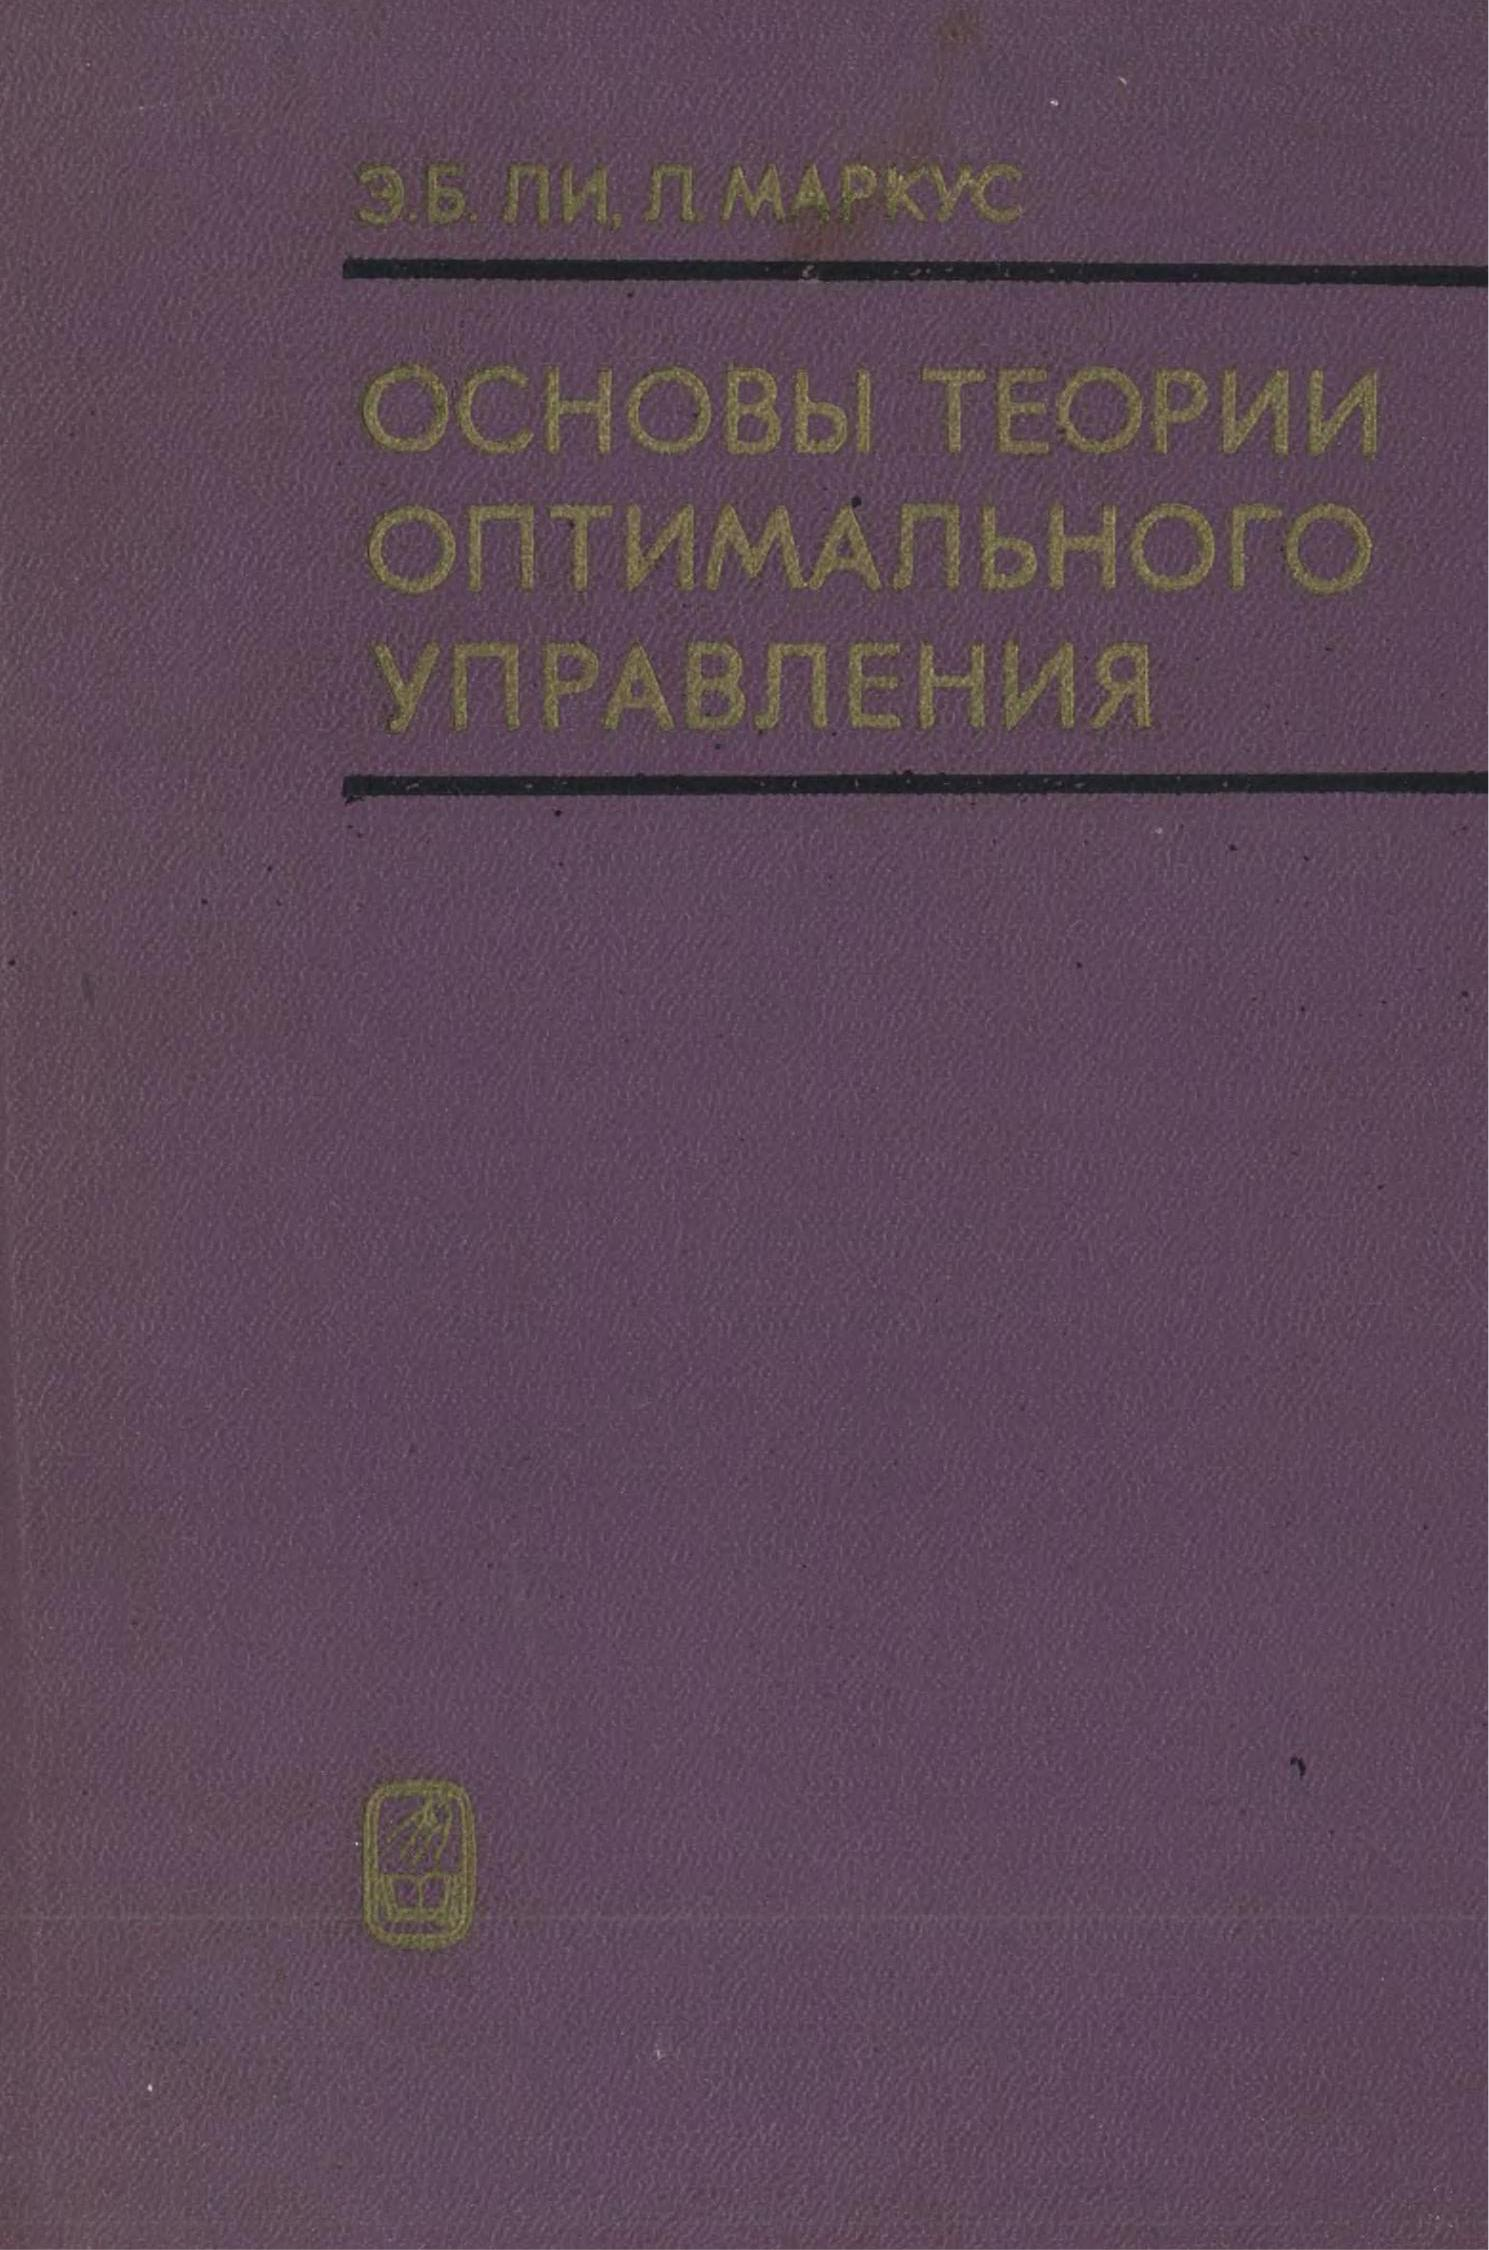
\includegraphics[max width=1.0\textwidth]{images/bo_d547k8bef24c73bgfcg0_0_0_87_1489_2250_0.jpg}
\end{center}
\hspace*{3em} 

\section*{ОСНОВЫ ТЕОРИИ ОПТИМАЛЬНОГО УПРАВЛЕНИЯ}

Перевод с английского Л. Л. ЛЕОНТЬЕВОЙ

Под редакцией Я. Н. РОЙТЕНБЕРГА

ИЗДАТЕЛЬСТВО «НАУКА»

ГЛАВНАЯ РЕДАКЦИЯ

ФИЗИКО-МАТЕМАТИЧЕСКОЙ ЛИТЕРАТУРЫ

МОСКВА 1972

6ф6.5

Л 55

УДК 62-52

Основы теории оптимального управления, Ли Э. Б., Маркус Л., перев. с англ., Главная редакция физико-математической литературы изд-ва «Наука», М., 1972, 576 стр.

Фундаментальный труд по математической теории оптимального управле- ния, в котором изложение проводится последовательно с позиций качественной теории дифференциальных уравнений.

Дается постановка задачи оптимального управления детерминированными системами, излагается теория оптимального управления линейными системами. Рассматриваются теория оптимальных линейных управляемых систем с инте- гральным выпуклым критерием качества, принцип максимума Л. С. Понтрягина, вопросы существования оптимальных управлений для нелинейных систем, достаточные условия оптимальности. Исследуются вопросы управляемости, наблюдаемости и устойчивости управляемых систем. Изучается синтез нели- нейных управляемых систем.

Книга рассчитана на инженеров и научных работников, занятых исследо- ванием и проектированием автоматических систем, а также на математиков.

Илл. 35. Библ. назв. 267.

FOUNDATIONS OF OPTIMAL CONTROL THEORY

E. B. Lee

L. Markus

Center for Control Sciences Institute of Technology University of Minnesota

John Wiley \& Sons, Inc., New York, London, Sydney

оглавление

Предисловие авторов к русскому изданию 5

Предисловие 7

Глава 1. Теория, методы и примеры синтеза оптимального управления 9

1.1. Примеры задач оптимального управления 9

1.2. Постановка общей задачи оптимального управления 31

1.3. Основные результаты теории управляемости 39

1.4. Экстремальные свойства оптимальных управлений и их синтез 44

1.5. Синтез оптимальных управлений для линейных систем второго порядка 48

Приложение I. Геометрическая теория обыкновенных дифферен- циальных уравнений 59

Приложение II. Алгебраическая теория линейных дифференциаль- ных уравнений 68

Глава 2. Оптимальное управление в линейных системах 76

2.1. Линейные управляемые процессы 76

2.2. Управляемость: множество достижимости 77

2.3. Управляемость и устойчивость автономных систем 91

2.4. Управляемость и наблюдаемость 115

2.5. Оптимальное по быстродействию управление для линейных систем 138

Приложение. Выпуклые множества 168

Глава 3. Оптимальное управление для линейных систем с инте- гральным выпуклым критерием качества 183

3.1. Значение интегрального критерия качества 183

3.2. Интегральный квадратичный критерий качества 184

3.3. Иллюстрирующие примеры и специальные задачи 204

3.4. Интегральный выпуклый критерий качества 223

3.5. Интегральный выпуклый критерий качества при ограниченных управлениях 252

Глава 4. Принцип максимума и существование оптимальных управ- лений для нелинейных систем 262

4.1. Геометрия множества достижимости 262

4.2. Существование оптимального управления при дополнительных ограничениях 284

4.3. Существование оптимального управления без дополнительных ограничений 313

Глава 5. Необходимые и достаточные условия оптимального управления 336

5.1. Принцип максимума и условия трансверсальности как необхо- димые условия 336

5.2. Достаточные условия оптимальности управления 372

Глава 6. Свойства управляемых систем: управляемость, наблюдаемость и устойчивость 397

6.1. Управляемость и наблюдаемость для нелинейных процессов 6.2. Глобальная устойчивость нелинейных процессов 397

429

Глава 7. Синтез оптимальных управлений для некоторых основных нелинейных управляемых систем 458

7.1. Синтез оптимальных по быстродействию управлений с обрат- ной связью для нелинейных систем второго порядка с одной степенью свободы 460

7.2. Оптимальное управление метеорологической ракетой 489

7.3. Управление угловой скоростью твердого тела 499

7.4. Оптимальная астронавигация 507

Приложение А. Метод наискорейшего спуска и другие численные методы в задачах оптимального управления 515

A1. Метод наискорейшего спуска 516

A2. Применение метода наискорейшего спуска к зада- чам оптимального управления и формулировка вычислительных алгоритмов 525

А3. Работы по методу наускорейшего спуска и вычисли- тельным методам оптимального управления 549

Библиография к приложению А 550

Прилоржение Б. Работы по оптимальному управлению системами, описываемыми обыкновенными дифференциальны- ми уравнениями и уравнениями в частных произ- водных 555

Б1. Управляемые системы, описываемые функциональ- но-дифференциальными уравнениями или уравнени. ями в частных производных, и применимость функционального анализа 555

Б2. Абстрактный принцип максимума 559

Б3. Краткий указатель к библиографии 561

Библиография к приложению Б 563

Литература 566

Предметный указатель 572

\section*{предисловие Авторов к русскому изданию}

Математической основой теории оптимального управления являются такие области математики, как теория дифференциаль- ных уравнений и вариационное исчисление, истоки развития кото- рых связаны с именем ееличайшего математика восемнадцатого столетия, петербургского академика Л. Эйлера.

В Советском Союзе после Великой Отечественной войны раз- витие современных методов в соответствующих разделах клас. сической математики и механики было вызвано к жизни потреб- ностями таких новых областей науки и техники, как освоение космического пространства, сверхзвуковая авиация и автоматиза- ция управления производственными процессами с применением вычислительных машин. Блестящее открытие академика Л. С. Понт- рягина и его сотрудников — принцип максимума — дает строгое математическое обоснование теории оптимального управления, отвечающей запросам новой техники. В настоящее время совет- ские ученые принимают активное участие в разработке и при- менении современных методов оптимального управления.

Co времени опубликования первого издания книги в 1967 г. исследования в области управления детерминированными систе- мами (стохастическое управление в книге не рассматривалось) далеко продвинулись вперед. Основные направления новейших исследований указаны в приложениях А и Б. В частности, важные результаты получены в теории управления системами с запазды- ванием, системами, описываемыми функциональными уравнениями, а также уравнениями в частных производных. Получили разви- тие также приложения теории дифференциальных игр.

Bce эти теоретические изыскания находят все более широкое применение в инженерной практике. С помощью быстродействую- щих вычислительных машин производится непосредственное авто- матическое управление химическими и механическими процессами. Не менее важной представляется роль теории управления в планировании и проектировании различных производственных предприятий.

Авторы выражают благодарность издательству «Наука» Ака- демии наук CCCP за предоставленную им возможность принять участие в подготовке русского издания. Мы благодарим также профессора Я. Н. Ройтенберга и его сотрудников за тщательный перевод и подготовку русского издания книги, в которую внесен ряд исправлений по сравнению с американским изданием. Однако каждый из авторов сознает, что вся ответственность за возмож- ные неточности лежит на нем и его соавторе.

Миннеаполис, Миннесота, 1971.

9. Б. Ли, Л. Маркус

\section*{предисловие}

Математическая теория оптимального управления зародилась около двадцати лет назад в качестве специального отдела теории дифференциальных уравнений. После того как были установлены принцип максимума и метод динамического программирования, появилась тенденция рассматривать теорию оптимального управ- ления в рамках вариационного исчисления. Однако многие из основных понятий теории управления базируются на качествен- ной теории дифференциальных уравнений, и наше изложение ис- ходит именно из такого подхода.

За последние три или четыре года теория управления для детерминированных процессов со многими степенями свободы достигла вполне удовлетворительной стадии завершенности. Фундаментальные задачи теории управления, рассматриваемые с точки зрения теории нелинейных обыкновенных дифференциаль- ных уравнений, получили как точную математическую формули- ровку, так и строгое решение.

Именно в силу полноты и разработанности этой теории ав- торы настоящей книги полагают, что подробное изложение ее современного состояния послужит хорошей основой для дальней- ших исследований в этой области. Такова и была цель написа- ния «Основ теории оптимального управления». В нашу задачу входило систематическое изложение теории управления, достаточно полное и подробное, однако не выходящее за пределы рассмотре- ния детерминированных (не стохастических) систем, описываемых обыкновенными дифференциальными уравнениями.

Книга выдержана в основном в строгом математическом стиле определений, теорем и доказательств. Каждое аналитическое или геометрическое заключение базируется на предварительно обосно- ванных предположениях. В некоторых случаях, однако, ограниче- ния, накладываемые на системы, например, непрерывность или ограниченность, перечисляются в начале раздела, а затем уже считаются само собой разумеющимися, что следует иметь в виду при изучении. Почти после каждого раздела следуют упражне- ния. Некоторые из них являются простыми задачами, иллюстри- рующими материал, другие содержат уточнения и продолжения изложенного; иногда в упражнении дается какая-либо деталь доказательства (или вычислений) одной из теорем текста.

Для чтения настоящей книги необходимо знание курса тео- рии дифференциальных уравнений и математического анализа. Естественно, что для читателя, владеющего основами теории функций и методами теории управления линейных систем, изу- чение книги будет значительно облегчено.

Ряд замечаний и полезных советов были высказаны доктором Шаком, доктором Гарвеем и мистером Стоуном. Некоторые раз- делы текста обсуждались с доктором Вильсоном и мистером Голлвитцером. Однако каждый из авторов еще раз подтверждает, что вся ответственность за возможные ошибки и неточности лежит исключительно на нем и его соавторе.

TEOPИЯ, МЕТОДЫ И ПРИМЕРЫ СИНТЕЗА оптимАльного УПРАВЛEHИЯ

В этой главе изложена общая теория оптимального управления для линейных и нелинейных систем и описывается применение ее основных принципов в задачах синтеза оптимальных регуляторов. Последовательнсе математическое развитие этих идей дается в пос- ледующих главах. Мы будем рассматривать только непрерывные детерминированные системы, хотя многие из полученных резуль- татов применимы и для стохастических систем управления.

\section*{1.1. Примеры задач оптимального управления}

Конструирование оптимальных систем управления обычно при- водит к появлению нелинейных зависимостей, и поэтому существен- но отличается от исследования элементарных линейных систем с обратной связью. Исследуя некоторые примеры, мы введем основ- ные понятия и опишем методы теории оптимального управления.

П р име p 1. Управление угловой скоростью ротора. Рассмот. рим диск или ротор R, свободно вращающийся вокруг неподвиж- ной оси, проходящей через центр тяжести диска и перпендикуляр- ной к его плоскости. Пусть ω(t) — угловая скорость ротора в момент времени t, причем в начальный момент времени ω (0) \(= {\omega }_{0}\) и пусть требуется остановить ротор. Таким образом, задача сос- тоит в том, чтобы осуществить управление величиной ω (t) (выход- ной величиной системы), приводя ее от ω = ω, до ω = 0 с помощью приложения некоторого внешнего момента L (t) к оси вращения.

Уравнение движения ротора имеет вид

\[
I\frac{d\omega }{dt} = L\left( t\right)
\]

где I —момент инерции ротора относительно оси вращения (I — пос- тоянная положительная величина), а L (t)—момент внешних сил — есть входная величина, или управление. Математически задача состоит в выборе такого \(L\left( t\right)\) , ссвместимого с механическим смыс- лом задачи, чтобы выход системы ω (t), являющийся решением указанного дифференциального уравнения с начальными условиями \(\omega \left( 0\right)  = {\omega }_{0}\) , CTремился к нулю с возрастанием времени. Более того, мы хотим выбрать управление \({L}^{ * }\left( t\right)\) , oбладающее свойством опти- мальности, такое, чтобы соответствующий ему выход достигал нуля наиболее эффективным образом, например, за минимально воз- можное время. Такая задача управления может возникнуть, на- пример, в случае, когда R представляет собой приводной шкив в некотором технологическом процессе, либо при управлении ракет- ным снарядом, где R — попереч. ное сечение снаряда. В первом случае управляющий момент мо- жет быть создан с помощью не- которого электромеханического устройства, во втором же слу- чае— при помощи вспомогатель- ныx реактивных двигателей. Задача о приведении величины \(\omega\) OT значения \(\omega  = {\omega }_{0}\) K \(\omega  = 0\) может возникнуть также в слу- чае, когда существует некоторая идеальная постоянная угловая скорость ротора R, так как при этом о можно интерпретировать как величину рассогласования между действительной и идеальной угловой скоростью. Таким образом, наш пример мог бы быть рассмотрен с общих позиций задачи о приведении рассогласова- ния к нулю. Если начальная угловая скорость од известна заранее, то управляющий сигнал удобно задавать как входной сигнал разомкнутой цепи (рис. 1.1, а) и искать управление L* (t), оптималь- ное по отношению к нашему критерию.

\begin{center}
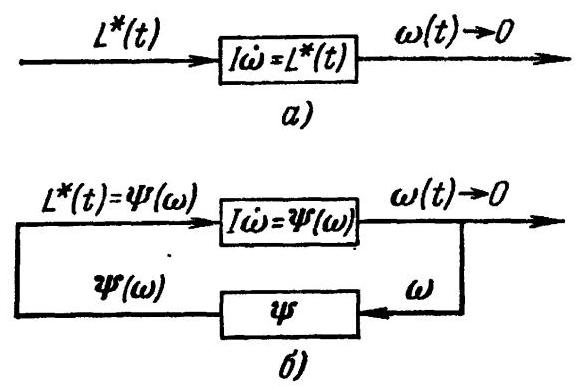
\includegraphics[max width=0.5\textwidth]{images/bo_d547k8bef24c73bgfcg0_10_209_598_580_388_0.jpg}
\end{center}
\hspace*{3em} 

Рис. 1.1. Cxema процесса управления: а) разомкнутая цепь, б) замкнутая цепь.

Если мы, однако, хотим сконструировать самокорректирующееся управляющее устройство, удовлетворительно функционирующее при всех возможных начальных значениях о, а также при воз- мушениях ω(t), то оптимальное управление L* (t) придется синте- зировать в форме соответствующего контура с обратной связью (см. рис. 1.1, б). А именно, мы должны вычислить некоторую функцию Ψ(ω) и использовать ее как управляющий сигнал в цепи обратной связи. Тогда решение ω(t) уравнения

\[
I\frac{d\omega }{dt} = \Psi \left( \omega \right)
\]

для каждого начального значения ω, будет оптимальным, т. е. \(\omega \left( t\right)\) совпадет с оптимальным решением очем ночное появилось бы на выходе разомкнутой цепи при оптимальном управлении \({L}^{ * }\left( t\right)\) .

Рассмотрим линейный сигнал в цепи обратной связи вида

\[
\Psi \left( \omega \right)  =  - {k\omega },
\]

где k > 0—постоянный коэффициент усиления. Тогда уравнение

\[
I\dot{\omega } =  - {k\omega },\;\omega \left( 0\right)  = {\omega }_{0}
\]

имеет решение

\[
\omega \left( t\right)  = {\omega }_{0}{e}^{-\frac{k}{I} \cdot  t}
\]

стремящееся к нулю при \(t \rightarrow  \infty\) . Если мы хотим ускорить тормо- жение \(\omega \left( t\right)\) , to нужно увеличить коэффициент усиления k; однако, каким бы большим ни был коэффициент к в этой математической мо- дели, ротор окончательно не остановится —он только стремится к состоянию покоя. Более того, проблема выбора оптимального линей. ного управления с обратной связью в такой постановке не имеет решения, ибо каждое такое управление можно улучшить, увели- чивая коэффициент усиления. Кроме того, задача поставлена и физически неудовлетворительно, так как в действительности су- ществует предел увеличения коэффициента усиления в цепи обрат- ной связи, ибо возникающие нелинейности типа насыщения сильно влияют на характеристики цепи. Для оптимального управления ротором разумно было бы потребовать, чтобы управляющий момент был заключен в некоторых границах. Для простоты обозначений положим

\[
- 1 \leq  L\left( t\right)  \leq  1\text{ . }
\]

Управляющий момент L*(t), который не обязан изменяться не- прерывно (допускаются мгновённые переключения), должен удов- летворять ограничению \(\left| {{L}^{ * }\left( t\right) }\right|  \leq  1\) и переводить о из начального состояния \(\omega  = {\omega }_{0}\) в желаемое состояние ω \(= 0\) за минимальное воз- можное время. Решение для оптимального по быстродействию управления \({L}^{ * }\left( t\right)\) в разомкнутой цепи очевидно из физических соображений. Если ω₁＞0, то положнм

Toraa

\[
{L}^{ * }\left( t\right)  =  - 1\text{ . }
\]

\[
{\omega }^{ * }\left( t\right)  = \frac{I{\omega }_{0} - t}{I}
\]

при \(t \leq  T = I{\omega }_{0}\) и \({\omega }^{ * }\left( T\right)  = 0\) . Если \({\omega }_{0} < 0\) ,то положим \({L}^{ * }\left( t\right)  =\) =+1 . Тогда

\[
{\omega }^{ * }\left( t\right)  = \frac{I{\omega }_{0} + t}{I}
\]

при \(t \leq  T =  - I{\omega }_{0}\) и \({\omega }^{ * }\left( T\right)  = 0\) . Так как оптимальный выход \({\omega }^{ * }\left( t\right)\) имеет постоянный знак, то легко построить синтезирующую функ- цию \(\Psi \left( \omega \right)\) для цепи обратной связи. Положим \(\Psi \left( \omega \right)  =  - \operatorname{sgn}\omega\) ,где

\[
\operatorname{sgn}\omega  = \begin{cases}  + 1 & {\text{ п }\text{ р }\text{ н }\omega } > 0, \\  0 & {\text{ п }\text{ р }\text{ н }\omega } = 0, \\   - 1 & {\text{ п }\text{ р }\text{ н }\omega } < 0. \end{cases}
\]

Тогда нелинейное дифференциальное уравнение

\[
{I\omega } =  - \operatorname{sgn}\omega
\]

для каждого начального значения о, будет иметь решение, совпа- дающее с оптимальным выходом ω* (t) для соответствующей разомк- нутой системы.

П р име p 2. Управление механизмом, движущимся по гладким рельсам. Рассмотрим механизм массы m, например, тележку, ко- торая движется по горизонтальным рельсам с ничтожно малым трением. Координата х положения тележки в момент времени t определяется по закону Ньютона

\[
m\ddot{x} = u\left( t\right) ,
\]

где \(u\left( t\right)  - {u3}\) меряемая в соответствующих единицах внешняя управ- ляющая сила, приложенная к тележке. Предположим, что началь- ное положение и начальная скорость тележки заданы: \(x = {x}_{0}\) и \(x = y = {y}_{0}\) . Рассмотрим задачу остановки тележки в предписанном положении, скажем, \(x = 0,y = 0,3\) а минимальное возможное вре- мя с помощью управляющей силы и (t) (возможно, разрывной), удовлетворяющей ограничению

\[
\left| {u\left( t\right) }\right|  \leq  1\text{ . }
\]

Здесь решение задачи синтеза оптимального управления не оче- видно, и полученный ниже результат будет неожиданным. Методы, вкратце изложенные в связи с этой задачей, составят основное содержание главы 2, где дается также строгое доказательство не- которых геометрических соотношений, используемых здесь чисто интуитивно. Изложение этого примера будет довольно простран- ным, ибо он иллюстрирует один из основных подходов к задаче управления.

Для удобства примем массу m равной единице, и, обозначая скорость \(x = y\) ,3апишем уравнение движения в виде системы двух дифференциальных уравнений первого порядка

\[
\dot{x} = y,\;\dot{y} = u\left( t\right)
\]

или, в матричной форме,

\[
\left\lbrack  \begin{array}{l} x \\  y \end{array}\right\rbrack   = \left\lbrack  \begin{array}{ll} 0 & 1 \\  0 & 0 \end{array}\right\rbrack  \left\lbrack  \begin{array}{l} x \\  y \end{array}\right\rbrack   + \left\lbrack  \begin{array}{l} 0 \\  1 \end{array}\right\rbrack  u\left( t\right)
\]

T. e.

\[
\dot{\mathbf{x}} = A\mathbf{x} + {bu},
\]

где \(\mathbf{x} = \left\lbrack  \begin{array}{l} x \\  y \end{array}\right\rbrack   -\) вектор, \(A = \left\lbrack  \begin{array}{ll} 0 & 1 \\  0 & 0 \end{array}\right\rbrack\) и \(b = \left\lbrack  \begin{array}{l} 0 \\  1 \end{array}\right\rbrack   -\) матрицы.Вэтомпри- мере наиболее важные формулы будут представлены как в коор- динатной, так и в матричной форме.

Удобно рассматривать решение

\[
\mathbf{x}\left( t\right)  = \left\lbrack  \begin{array}{l} x\left( t\right) \\  y\left( t\right)  \end{array}\right\rbrack
\]

как кривую, заданную параметрически в плоскости ху, называе- мой фазовой плоскостью. Таким образом, мы выбираем некоторое управление \(u\left( t\right)\) c orраничением \(\left| {u\left( t\right) }\right|  \leq  1\) , u затем исследуем соответствующее решение \(x\left( t\right)\) , удовлетворяющее начальным усло- виям \({x}_{0} = \left\lbrack  \begin{array}{l} {x}_{0} \\  {y}_{0} \end{array}\right\rbrack\) . При этом наша цель заключается в перемещении механизма из состояния х, в состояние х = 0 за минимальное воз- MOXKHOE BPEMA.

\({\Phi }_{\text{ HKCHpyeM MOMeHT BpeMeHH }}{t}_{1} > 0\) и рассмотрнм все возможные управления \(u\left( t\right)\) на интервале времени \(0 \leq  t \leq  {t}_{1}\) с ограниче- нием \(\left| {u\left( t\right) }\right|  \leq  1\) . Каждое изэтнх управлений определяет соотвег- ствующее решение \(x\left( t\right)\) ,нсходящее из заданной точки \({x}_{0}\) . Непо- средственной подстановкой легко проверить, что решение опреде- ляется формулами

\[
x\left( t\right)  = {x}_{0} + {y}_{0}t + {\int }_{0}^{t}\left\lbrack  {{\int }_{0}^{s}u\left( \sigma \right) {d\sigma }}\right\rbrack  {ds},
\]

\[
y\left( t\right)  = {y}_{0} + {\int }_{0}^{t}u\left( \sigma \right) {d\sigma }
\]

HЛИ

\[
\mathbf{x}\left( t\right)  = {e}^{At}{\mathbf{x}}_{0} + {e}^{At}{\int }_{0}^{t}{e}^{-{As}}{bu}\left( s\right) {ds}.
\]

Определим подмножество \(K\left( {t}_{1}\right)\) на фазовой плоскости как совокуп- ность конечных точек всех описанных выше траекторий, имеющих начало при \(t = 0\) в точке х,. Другими словами, \(K\left( {t}_{1}\right)\) представляет собой множество тех точек, которые могут быть достигнуты за время \({t}_{1}\) , если исходить из начального состояния х, под действием управлений, удовлетворяющих нашим ограничениям. В рассматри- ваемом примере нетрудно проверить (а далее в общей теории это доказывается), что \(K\left( {t}_{1}\right)\) — ограниченное замкнутое выпуклое мно- жество,непрерывно зависящее от \({t}_{1}\) .

Оптимальное время t=t* определяется, как первый момент времени, при котором множество \(\dot{K}\left( t\right)\) будет содержать точку (0,0). Ввиду того, что K(t) непрерывно зависит от t, можно доказать, что точка \(\left( {0,0}\right)\) лежит на границе множества K(t*). Оптималь- ная траектория \({\mathbf{x}}^{ * }\left( t\right)  = \left\lbrack  \begin{array}{l} {x}^{ * }\left( t\right) \\  {y}^{ * }\left( t\right)  \end{array}\right\rbrack\) приводит в начало координат в момент \(t = {t}^{ * }\) , a оптимальное управление \({u}^{ * }\left( t\right) ,0 \leq  t \leq  {t}^{ * } -\) это то управление, которое порождает эту оптимальную траекторию.

Пусть \(\eta \left( {t}^{ * }\right)  = \left( {{\eta }_{1}\left( {t}^{ * }\right) ,{\eta }_{2}\left( {t}^{ * }\right) }\right)\) —постоянный единичный вектор,

т. e. вектор \(\mathbf{x}\left( {t}^{ * }\right)\) ,идущий из начала координат в точку х (t*), не имеет положительной состав- ляющей вдоль направления внеш- ней нормали; это представляет собой аналитическое выражение того факта, что η(t*) является внешней нормалью множества исходящий из начала координат и направленный по внешней нор- мали к выпуклому множеству \(K\left( {t}^{ * }\right)\) (puc. 1.2). Тогда для каж- дой траектории \(x\left( t\right)  = \left( \begin{array}{l} x\left( t\right) \\  y\left( t\right)  \end{array}\right)\) , приводящей в точку х(t*) ∈ K(t*), должно выполняться условие

\[
{\eta }_{1}\left( {t}^{ * }\right) x\left( {t}^{ * }\right)  + {\eta }_{2}\left( {t}^{ * }\right) y\left( {t}^{ * }\right)  \leq  0
\]

\begin{center}
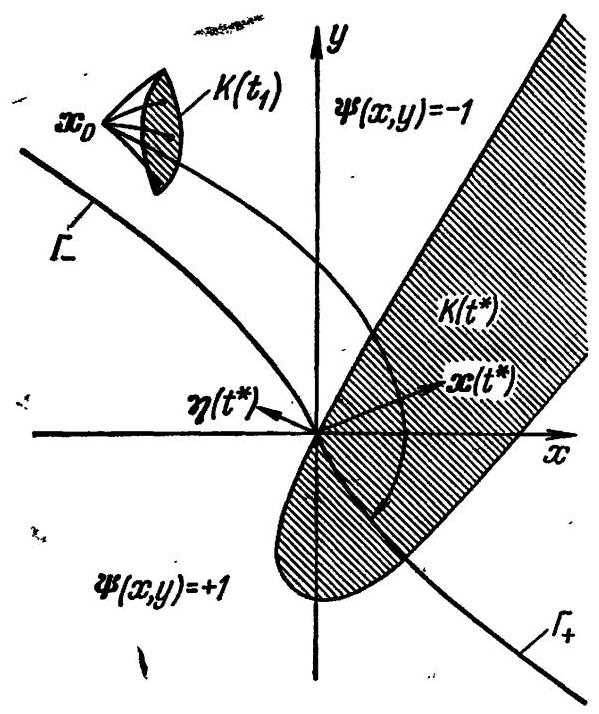
\includegraphics[max width=0.5\textwidth]{images/bo_d547k8bef24c73bgfcg0_14_161_390_599_714_0.jpg}
\end{center}
\hspace*{3em} 

Рис. 1.2. Множество достижимости и кри- вая переключений для системы х=и, \(\left| {u\left( t\right) }\right|  \leq  1\) .

ИЛИ

\[
\eta \left( {t}^{ * }\right) x\left( {t}^{ * }\right)  \leq  0,
\]

\(K\left( {t}^{ * }\right)\) в граничной точке х* (t*) = 0 :

\[
{\eta }_{1}\left( {t}^{ * }\right) {x}^{ * }\left( {t}^{ * }\right)  + {\eta }_{2}\left( {t}^{ * }\right) {y}^{ * }\left( {t}^{ * }\right)  = \mathop{\max }\limits_{{\left( {{x}_{0}y}\right)  \in  K\left( {t}^{ * }\right) }}\left( {{\eta }_{1}\left( {t}^{ * }\right) x + {\eta }_{2}\left( {t}^{ * }\right) y}\right) ,
\]

HJIM

\[
\eta \left( {t}^{ * }\right) {\mathbf{x}}^{ * }\left( {t}^{ * }\right)  = \max \eta \left( {t}^{ * }\right) \mathbf{x}\left( {t}^{ * }\right) .
\]

В этом последнем равенстве, являющемся выражением так назы- ваемого принципа максимума, максимум берется по всем траек- ториям x(t), приводящим в точку x (t*) Е К (t*). Далее мы выведем из принципа максимума некоторые экстремальные свойства опти- мального управления \({u}^{ * }\left( t\right)\) и построим функцию \(\Psi \left( {x,y}\right)\) ,на основании которой осуществляется синтез. Поскольку в принципе максимума участвуют оптимальное время t* и вектор нормали η(t*), заранее не известные, то мы будем применять его неявно.

Используя интегральное выражение для х (t), представим левую часть предыдущего соотношения в виде

\[
{\eta }_{1}\left( {t}^{ * }\right) \left\lbrack  {{x}_{0} + {y}_{0}{t}^{ * } + {\int }_{0}^{{t}^{ * }}{\int }_{0}^{s}u\left( \sigma \right) {d\sigma ds}}\right\rbrack   + {\eta }_{2}\left( {t}^{ * }\right) \left\lbrack  {{y}_{0} + {\int }_{0}^{{t}^{ * }}u\left( \sigma \right) {d\sigma }}\right\rbrack  .
\]

Если рассматривать лишь те члены этого выражения, которые содержат и (t), то получим, что выражение

\[
{\eta }_{1}\left( {t}^{ * }\right) {\int }_{0}^{{t}^{ * }}{\int }_{0}^{s}u\left( \sigma \right) {d\sigma ds} + {\eta }_{2}\left( {t}^{ * }\right) {\int }_{0}^{{t}^{ * }}u\left( \sigma \right) {d\sigma }
\]

должно достигать максимума при оптимальном управлении и*(t). Учитывая тождество, которое можно проверить дифференцированием,

\[
{\int }_{0}^{t}{\int }_{0}^{s}u\left( \sigma \right) {d\sigma ds} = {\int }_{0}^{t}\left( {t - \sigma }\right) u\left( \sigma \right) {d\sigma },
\]

и полагая \({\eta }_{1}\left( s\right)  = {\eta }_{1}\left( {t}^{ * }\right) ,{\eta }_{2}\left( s\right)  = {\eta }_{1}\left( {t}^{ * }\right) \left( {{t}^{ * } - s}\right)  + {\eta }_{2}\left( {t}^{ * }\right)\) на интерва- ле \(0 \leq  s \leq  {t}^{ * }\) , noлучим,что управление \({u}^{ * }\left( t\right)\) максимизирует инте- грал

\[
{\int }_{0}^{{t}^{ * }}{\eta }_{2}\left( s\right) u\left( s\right) {ds}
\]

В матричной записи проведенные выше выкладки означают, что и* (t) максимизирует выражение

\[
\eta \left( {t}^{ * }\right) {e}^{{At} * }{\mathbf{x}}_{0} + \eta \left( {t}^{ * }\right) {e}^{{At} * }{\int }_{0}^{{t}^{ * }}{e}^{-{As}}{bu}\left( s\right) {ds},
\]

так что \({u}^{ * }\left( t\right)\) макснмизирует также второй член

\[
{\int }_{0}^{{t}^{ * }}\eta \left( s\right) {bu}\left( s\right) {ds} = {\int }_{0}^{{t}^{ * }}{\eta }_{2}\left( s\right) u\left( s\right) {ds},
\]

где

\[
\eta \left( {t}^{ * }\right) {e}^{{At} * }{e}^{-{As}} = \eta \left( s\right)  = \left( {{\eta }_{1}\left( s\right) ,{\eta }_{2}\left( s\right) }\right) .
\]

Учитывая условие \(\left| {u\left( t\right) }\right|  \leq  1\) ,легко понять, что максимум инте- грала

\[
{\int }_{0}^{t * }{\eta }_{2}\left( s\right) u\left( s\right) {ds}
\]

достигается при управлении

\[
{u}^{ * }\left( t\right)  = \operatorname{sgn}{\eta }_{2}\left( t\right) \;\left( {0 \leq  t \leq  {t}^{ * }}\right) .
\]

Таким образом, оптимальное управление и * (t) является релей- ным управлением, т. е., оно принимает значения, равные +1 и — 1, за исключением тех точек, где происходит переключение, а именно, нулей неизвестной функции \({\eta }_{2}\left( t\right)\) .

Однако из определения η(t) видно, что

\[
{\dot{\eta }}_{1} = 0,\;{\dot{\eta }}_{2} =  - {\eta }_{1},
\]

или, в матричной записи,

Поэтому

\[
\dot{\mathbf{\eta }}\left( t\right)  = \mathbf{\eta }\left( {t}^{ * }\right) {e}^{A{t}^{ * }}{e}^{-{At}}\left( {-A}\right)  =  - \mathbf{\eta }\left( t\right) A.
\]

\[
{\ddot{\eta }}_{2} = 0
\]

и \({\eta }_{2}\left( t\right)\) является линейной функцией от t. Отсюда заключаем, что \({\eta }_{2}\left( t\right)\) имеет не более одного нуля. Итак, оптимальное управление \({u}^{ * }\left( t\right)\) есть релейное управление со значениями + 1 и - 1 и не бо- лее, чем с одним переключением. Используя этот факт, мы можем построить функцию \(\Psi \left( {x,y}\right)\) , ocyществляющую синтез в рассматри- ваемой задаче.

Оптимальная траектория движения, начинающаяся в точке х, и идущая в начало координат, должна сначала совпадать с парабо- лой, являющейся решением системы

\[
\left( {\mathcal{G}}_{ - }\right)
\]

\[
\dot{x} = y,\;\dot{y} =  - 1\;\left( {u \equiv   - 1}\right) ,
\]

а затем с параболой, являющейся решением системы

\[
\left( {\mathcal{S}}_{ + }\right)
\]

\[
\dot{x} = y,\;\dot{y} =  + 1\;\left( {u \equiv   + 1}\right)
\]

или наоборот. Так как экстремальные системы дифференциальных уравнений \({\mathcal{S}}_{ + }\) и \({\mathcal{S}}_{ - }\) автономны (их коэффициенты не зависят от времени), то экстремальные траектории могут быть построены сле- дующим образом. Начиная экстремальное движение в момент t = 0 из начала координат, движемся по траекториям решений систем £\_ и \$\_ в обратном направлении (попятное движение), чтобы до- стичь точки х, в некоторый отрицательный момент \(t =  - {t}^{ * }\) . Меняя порядок отсчета времени на обратный, мы начинаем движение из \({\mathbf{x}}_{0}\) при \(t = 0\) и достигаем начала координат при \(t = {t}^{ * }\) . Таким образом, нами получено оптимальное движение х*(*), оптималь- ное время t* и оптимальное управление и*(t).

Построим теперь все возможные экстремальные траектории, на- чинающиеся из произвольных точек и приводящие в начало коор- динат. Выберем единичный вектор \(\eta \left( 0\right)  = \left( {{\eta }_{1}\left( 0\right) ,{\eta }_{2}\left( 0\right) }\right)\) и исполь- зуем его в качестве начальных условий при решении системы

\[
{\dot{\eta }}_{1} = 0,\;{\dot{\eta }}_{2} =  - {\eta }_{1}.
\]

Пользуясь управлением и (t) = sgn \({\eta }_{2}\left( t\right)\) для определения экстре- мальной траектории, приходящей в начало координат при t=0, построим решение системы

\[
\dot{x} = y,\;\dot{y} = \operatorname{sgn}{\eta }_{2}\left( t\right)
\]

с начальными условиями \(x\left( 0\right)  = 0,y\left( 0\right)  = 0\) . Таким образом, мы сможем построить все возможные экстремальные траектории, ве- дущие в начало координат при возрастании t, в том числе и на- чинающуюся в точке \({\mathbf{x}}_{\mathbf{0}}\) . Если,например,взять \({\eta }_{1}\left( 0\right)  = 0,{\eta }_{2}\left( 0\right)  = \; =  + 1\) , to \({\eta }_{2}\left( t\right)  \equiv   + 1\) при \(t \leq  0,\) u движение происходит по траек- тории, удовлетворяющей системе

\[
\dot{x} = y,\;\dot{y} =  + 1
\]

или уравнению

\[
\frac{dy}{dx} = \frac{1}{y}
\]

рещеннем которого,как известно,является парабола (см. рис. 1.3)

\[
{\Gamma }_{ + } : {2x} = {y}^{2}\;\left( {y \leq  0}\right) .
\]

Аналогично при \({\eta }_{1}\left( 0\right)  = 0,{\eta }_{2}\left( 0\right)  =  - 1\) получим движение по пара- боле

\[
{\Gamma }_{ - } :  - {2x} = {y}^{2}\;\left( {y \geq  0}\right) .
\]

Для любых других значений \({\eta }_{1}\left( 0\right) ,{\eta }_{2}\left( 0\right)\) при \({\eta }_{2}\left( 0\right)  > 0\) движение происходит по траектории \({\Gamma }_{ + }\) до тех пор, пока ты не окажется равным нулю, а затем начинается движение в обратном направ- лении по некоторой траектории системы \$\_. Аналогичный процесс получим при \({\eta }_{2}\left( 0\right)  < 0\) . Простое изучение семейства интегральных кривых систем \(\mathcal{G}\) - и \({\mathcal{G}}_{ + }\) показывает,что для каждой заданной точки х, имеется один и только один экстремальный путь, приво- дящий в начало координат. Это экстремальное движение и будет оптимальным. Существование оптимального движения будет дока- зано в дальнейшем при изложении общей теории.

Кривая, составленная из \({\Gamma }_{ - }\) и \({\Gamma }_{ + }\) ,называется линией пере- ключения \(W\) . В нашем примере ее уравнение таково:

\[
y = W\left( x\right)  = \left\{  \begin{array}{ll}  - \sqrt{2x}. & \text{ при }x \geq  0, \\   + \sqrt{-{2x}} & \text{ при }x < 0. \end{array}\right.
\]

Определим синтезирующую функцию:

\[
\Psi \left( {x,y}\right)  = \begin{cases}  - 1, & \operatorname{ec\text{ л }\text{ н }}y > W\left( x\right) \text{ или если }\left( {x,y}\right)  \neq  \left( {0,0}\right) \text{ и } \\  0, & \operatorname{ec\text{ л }\text{ н }\text{ и }}x = y = 0, \\   + 1 & \operatorname{ec\text{ л }\text{ л }\text{ н }}y = W\left( x\right) \text{ илигалит }\Gamma , \\   + 1 & \operatorname{ec\text{ л }\text{ л }\text{ н }}y = W\left( x\right) \text{ илинелиг }\Gamma , \\   & \text{ принадлежит }{\Gamma }_{ + }. \end{cases}
\]

Тогда оптимальное движение из любого начального состояния \(\left\lbrack  \begin{array}{l} {x}_{0} \\  {y}_{0} \end{array}\right\rbrack\) в начало координат будет представлять собой решение урав- нения

\[
\ddot{x} = \Psi \left( {x,\dot{x}}\right)
\]

с начальными условиями \(x\left( 0\right)  = {x}_{0},\dot{x}\left( 0\right)  = {y}_{0}\) . Из геометрии фазо- вой плоскости следует, что, несмотря на разрывность функции

\(\Psi \left( {x,y}\right)\) при \(y = W\left( x\right)\) ,все решения уравнения \(\ddot{x} = \Psi \left( {x,\dot{x}}\right)\) опре- делены корректно. Функцию \(\Psi \left( {x,y}\right)\) , ocyществляющую синтез в этой задаче, можно эффективно реализовать в контуре обратной связи. На рис. 1.3 изображены оптимальные траектории системы

\[
\ddot{x} = u\left( t\right) ,\;\left| {u\left( t\right) }\right|  \leq  1
\]

при оптнмальном управлении

\[
{u}^{ * }\left( t\right)  = \Psi \left( {x\left( t\right) ,\dot{x}\left( t\right) }\right) .
\]

Оптимальное управление и* (t) для тележки можно интерпре- тировать как максимальную, ускоряющую силу, которая перехо-

Пример 3. Управление гармоническим осциллято- ром. Рассмотрим точку мас- сы т, положение которой в момент времени t опреде- ляется координатой \(x\) и на которую действует восста- навливающая сила — к’я дит затем в максимальную тормозящую силу, обеспе- чивающую остановку те- лежки в требуемой точке x = 0. Момент времени, ког- да совершается переход от ускорения к торможению (или наоборот), может быть найден графически. где постоянная \({k}^{2} > 0\) (например, \({k}^{2}\) — жесткость пружины). Урав- нение движения, согласно закону Ньютона имеет вид

\[
{mx} + {k}^{2}x = u\left( t\right) .
\]

\begin{center}
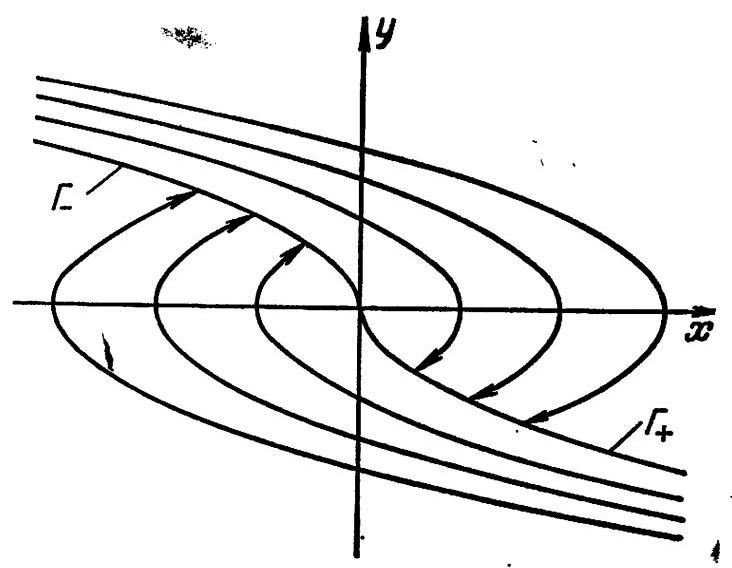
\includegraphics[max width=0.6\textwidth]{images/bo_d547k8bef24c73bgfcg0_18_184_703_732_568_0.jpg}
\end{center}
\hspace*{3em} 

Рис. 1.3. Оптимальные по быстродействию траек- Topни для системы x=y, y=u(t), \(\left| {u\left( t\right) }\right|  \leq  1\) .

Внешняя управляющая сила предполагается ограниченной по величине, скажем,

\[
\left| {u\left( t\right) }\right|  \leq  1\text{ . }
\]

Положим для простоты, что \(m = 1\mathrm{u}{k}^{2} = 1\) . Мы вновь хотим перевести объект из начального состояния \(x\left( 0\right)  = {x}_{0},\dot{x}\left( 0\right)  = {y}_{0}\) в начало координат за минимальное время. В фазовой плоскости соответствующая система дифференциальных уравнений имеет вид

\[
\dot{x} = y,\;\dot{y} =  - x + u\left( t\right)
\]

илн, в матрнчной записн,

\[
\dot{\mathbf{x}} = A\mathbf{x} + {bu}\left( t\right) ,
\]

где

\[
\mathbf{x}\left( t\right)  = \left\lbrack  \begin{array}{l} x\left( t\right) \\  y\left( t\right)  \end{array}\right\rbrack  ,\;A = \left\lbrack  \begin{array}{rr} 0 & 1 \\   - 1 & 0 \end{array}\right\rbrack  ,\;b = \left\lbrack  \begin{array}{l} 0 \\  1 \end{array}\right\rbrack  .
\]

Применяя те же рассуждения относительно выпуклого множества достижимости \(K\left( {t}_{1}\right)\) ,что и в предыдущем примере, мы придем к принципу максимума и получим формулу для оптимального управления:

\[
{u}^{ * }\left( t\right)  = \operatorname{sgn}{\eta }_{2}\left( t\right)
\]

где \(\eta \left( t\right)  = \left( {{\eta }_{1}\left( t\right) ,{\eta }_{2}\left( t\right) }\right)\) -решение системы

\[
{\dot{\eta }}_{1} = {\eta }_{2},\;{\dot{\eta }}_{2} =  - {\eta }_{l},
\]

ИЛИ

\[
\dot{\mathbf{\eta }}\left( t\right)  =  - \mathbf{\eta }A.
\]

Takнм образом,

\[
{\ddot{\eta }}_{2} + {\eta }_{2} = 0
\]

и \({\eta }_{2}\left( t\right)\) представляет собой гармоническое колебание. Промежуток времени между двумя последовательными нулями функции \({\eta }_{2}\left( t\right)\) равен π.

Построим линию переключения W и синтезирующую функцию \(\Psi \left( {x,y}\right)\) , paccматривая всевозможные экстремальные траектории, оканчивающиеся в начале координат. Мы должны исследовать се- мейства фазовых траекторий экстремальных систем дифференциаль- ных уравнений

\[
\left( {\mathcal{S}}_{ - }\right)
\]

\[
\dot{x} = y,\;\dot{y} =  - x - 1
\]

H

\[
\left( {\mathcal{S}}_{ + }\right)
\]

\[
\dot{x} = y,\;\dot{y} =  - x + 1.
\]

Интегральные кривые системы \$\_ представляют собой концентри- ческие окружности с центром в точке x= -1, y=0, с периодом обращения фазовой точки, равным 2π. Интегральные кривые си- стемы \({\mathcal{S}}_{ + }\) —окружности с центром в точке х= + 1, y=0 и с та- ким же периодом обращения фазовой точки.

Если выбрать единичный вектор η(0) так, чтобы η, 0 (0)=1, \({\eta }_{2}\left( 0\right)  = 0\) , to \({\eta }_{2}\left( t\right)  =  - \sin t\) и на интервале- \(\pi  < t < 0\) , sgn \({\eta }_{2}\left( t\right)  =\) = +1. Соответствующая экстремальная траектория совпадает с кривой, определяемой решением системы у., и проходит через на- чало координат. Ее уравнение

\[
{\Gamma }_{ + } : x =  - \cos t + 1,\;y = \sin t\;\left( {-\pi  < t < 0}\right)
\]

ИЛИ

\[
{\left( x - 1\right) }^{2} + {y}^{2} = 1,\;y < 0.
\]

Если \({r}_{11}\left( 0\right)  =  - 1,{\eta }_{2}\left( 0\right)  = 0\) , то \({\eta }_{2}\left( t\right)  = \sin t,u\) на интервале \(- \pi  < t < 0\) имеем sgn \({\eta }_{2}\left( t\right)  =  - 1\) . Соответствующая экстремаль- ная траектория совпадает с кривой, являющейся решением системы

Если выбрать теперь η(0) любым другим способом с тем, чтобы η2 (0) было положитель- ным, то в попятном движении экстремальная траектория -будет идти из начала коор- динат вдоль кривой \({\Gamma }_{ + }\) до S\_, и проходит через начало координат. Ее уравнение

\[
{\Gamma }_{ - } : x = \cos t - 1,\;y =  - \sin t
\]

\[
\left( {-\pi  < t < 0}\right)
\]

\begin{center}
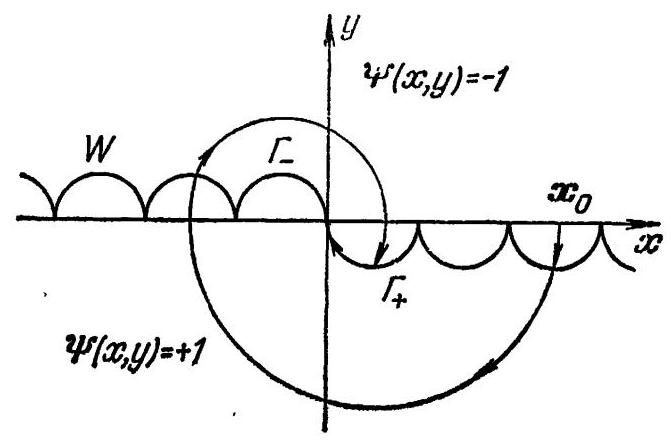
\includegraphics[max width=0.5\textwidth]{images/bo_d547k8bef24c73bgfcg0_20_189_540_671_441_0.jpg}
\end{center}
\hspace*{3em} 

Рис. 1.4. Оптимальное по быстродействию управление, приводящее систему х+х=и(t), \(\left| {u\left( t\right) }\right|  \leq  1\) в начало координат.

HANN

\[
{\left( x + 1\right) }^{2} + {y}^{2} = 1,\;y > 0.
\]

тех пор, пока дще (н) не станет равным нулю. В этой точке траек- тории экстремальное движение переключается на решение систе- мы \({\mathcal{S}}_{ - }\) ,по которому оно следует в течение промежутка времени π, до нового переключения на решение системы \$, (рис. 1.4). Ана- логичный процесс протекает при начальных условиях ца,(0) <0, но здесь экстремальная траектория возвращается из начала коор- динат вдоль кривой \({\Gamma }_{ - }\) .

Нетрудно в данном примере описать линию переключения, в точках которой происходит переключение между семействами решений \({\mathcal{L}}_{ - }u{\mathcal{L}}_{ + }\) .

Линия W состоит из дуг \({\Gamma }_{ + }\) и \({\Gamma }_{ - }\) и их последовательных сдвигов в обратном направлении вдоль соответствующих реше- ний систем \$\_ и \$\_ и \$ на промежутки времени продолжитель- ностью π. Например, дуга Г+ сдвигается в обратном направ- лении вдоль решений системы У. на промежуток времени т. Полу- чающийся образ дуги Г+ затем сдвигается (снова в обратном на- правлении) вдоль решений системы G+ на промежуток времени π и так далее. Заметим, что такой сдвиг вдоль решений си- стем £, или £\_ на промежуток π представляет собой поворот фазовой плоскости на угол π вокруг центра х=1, y=0 или \(x =  - 1,y = 0\) соответственно. В результате указанных преобра- зований дуг \({\Gamma }_{ + }\) и \({\Gamma }_{ - }\) возникает линия переключений W, состоя- цая из набора полуокружностей единичного радиуса, показанных на рис. 1.4.

Синтезирующая функция \(\Psi \left( {x,y}\right)\) при \(\left( {x,y}\right)  \neq  \left( {0,0}\right)\) имеет вид

\(\Psi \left( {x,y}\right)  = \left\{  \begin{array}{l}  - 1,\operatorname{ec\text{ л }\text{ и }}\left( {x,y}\right) \text{ лежит выше }W\text{ или на }{\Gamma }_{ - }, \\  0,\operatorname{ec\text{ л }\text{ и }}\left( {x,y}\right) \text{ лежит на }W, \\   + 1,\operatorname{ec\text{ л }\text{ и }}\left( {x,y}\right) \text{ лежит ниже }W\text{ или на }{\Gamma }_{ + }. \end{array}\right.\)

Оптимальные траектории управляемого гармонического осциллятора определяются решениями уравнения

\[
\ddot{x} + x = \Psi \left( {x,x}\right)
\]

для произвольного начального положения (х, у, о) фазовой точки. На рис. 1.4 изображены оптимальные траектории гармонического осциллятора. Качественно W можно определить на основе физи- ческого описания процесса управления, однако точный вид W и \(\Psi \left( {x,y}\right)\) может быть получен лишь в результате теоретического исследования, аналогичного проведенному выше.

Пример 4. Управление химической реакцией с нелинейным показателем качества. Пусть реагент А вводится с постоянной скоростью в реактор в течение определенного интервала времени \(0 \leq  t \leq  T\) . Предположим, что х есть значение величины рН, при которой протекает реакция, и которая определяет качество вы- ходного продукта; эта величина регулируется изменением концен- трации и какой-либо составляющей реагента А.

-Предположим, что реакция протекает таким образом, что ско- рость изменения х пропорциональна сумме текущего значения и концентрации и составляющей реагента A:

\[
\frac{dx}{dt} = {\alpha x} + {\beta u},
\]

где α и β—известные положительные постоянные. Далее предпо- ложим, что за меру изменения в выходе конечного продукта из-за вариаций pH принимается оценка

\[
{\int }_{0}^{T}{x}^{2}{dt}
\]

а расходы на поддержание соответствующей концентрации и про- порциональны и’. Тогда общая сумма расходов, связанная с уп- равлением \(u\left( t\right)\) на интервале 0 \(\leq  t \leq  T\) , onpeделяется выражением

\[
C\left( u\right)  = {\int }_{0}^{T}\left( {a{x}^{2} + {u}^{2}}\right) {dt}
\]

где \(a > 0\) - масштабный множитель. Теперь мы пришли к строгой математической формулировке задачи. При заданном начальном условии \(x\left( 0\right)\) требуется найти гуправляющую функцию и*(t) на интервале 0 ≤ \(i \leq  T\) так,чтобы определяемая ею функция \({x}^{ * }\left( t\right)\) доставляла минимум функционалу

\[
C\left( {u\left( t\right) }\right)  = {\int }_{0}^{T}\left\lbrack  {a{x}^{2}\left( t\right)  + {u}^{2}\left( t\right) }\right\rbrack  {dt}.
\]

Управляющая функция не является априори ограниченной, однако из неотрицательности подынтегральной функции следует, что существует некоторое оптимальное управление и*(t). Наша задача —осуществить синтез и*(t), т. е. определить оптимальное управление как функцию состояния \({x}^{ * }\left( t\right)\) .

Для этой цели можно воспользоваться принципом максимума, что и будет сделано в главе 3, однако при этом возникают неко- торые трудности из-за нелинейности функционала С (и). Здесь же мы используем другой путь, применив теорию динамического про- граммирования. Наши методы следуют принципу оптимальности, согласно которому из оптимальности управления и* (t) на участке \(0 \leq  t \leq  T\) следует его оптимальность на каждом подынтервале отрезка 0≤<t<t> <… Cтрогое обоснование этих методов базируется на понятии выпуклого множества достижимости и во многом сходно с анализом принципа максимума, который будет дан ниже.

Пусть в некоторый момент времени б, на интервале О ≤ < t < химическая реакция определяется состоянием х, пусть для ин- тервала [t, T] имеется оптимальное управление и *(t), дающее минимальные затраты \(V\left( {{x}_{0},{t}_{0}}\right)  = C\left( {u}^{ * }\right)\) . Для того чтобы дальней- шие рассмотрения были справедливы, будем считать функцию \(V\left( {x,t}\right)\) достаточно гладкой. Для каждого управления \(u\left( t\right)\) на \(\left\lbrack  {{t}_{0},T}\right\rbrack\) с соответствующим выходом \({x}_{a}\left( t\right)\) при начальном условии \({x}_{0}\) ве- личина затрат равняется

\[
{\int }_{{t}_{0}}^{{t}_{0} + \delta }\left\lbrack  {a{x}_{u}^{2}\left( t\right)  + {u}^{2}\left( t\right) }\right\rbrack  {dt} + {\int }_{{t}_{0} + \delta }^{T}\left\lbrack  {a{x}_{u}^{2}\left( t\right)  + {u}^{2}\left( t\right) }\right\rbrack  {dt},
\]

где \(\delta  > 0\) -сколь угодно малое число. Выбирая \(u\left( t\right)\) так, чтобы оно оптимизировало наш функционал на интервале [t, б, T], получим значение затрат:

\[
\mathop{\int }\limits_{{t}_{0}}^{{{t}_{0} + \delta }}\left\lbrack  {a{x}_{u}^{2}\left( t\right)  + {u}^{2}\left( t\right) }\right\rbrack  {dt} + V\left( {{x}_{u}\left( {{t}_{0} + \delta }\right) ,{t}_{0} + \delta }\right) .
\]

Но минимальное значение затрат при начальном значении \({x}_{0}\) в момент времени \({t}_{0}\) не превосходит этой величины,поэтому имеем

\[
V\left( {{x}_{0},{t}_{0}}\right)  = \mathop{\min }\limits_{{u\left( t\right) }}\left\{  {{\int }_{{t}_{0}}^{{t}_{0} + \delta }\left\lbrack  {a{x}_{u}^{2}\left( t\right)  + {u}^{2}\left( t\right) }\right\rbrack  {dt} + V\left( {{x}_{0}\left( {{t}_{0} + \delta }\right) ,{t}_{0} + \delta }\right) }\right\}  ,
\]

где мннимум берется по всем управлениям \(u\left( t\right)\) на \(\left\lbrack  {{t}_{0},T}\right\rbrack\) .Это уравнение иллюстрирует основную идею динамического програм- мирования, заключающуюся в том, что программа оптимального управления разбивается на сумму двух программ, действующих на интервалах \(\left\lbrack  {{t}_{0},{t}_{0} + \delta }\right\rbrack\) и \(\left\lbrack  {{t}_{0} + \delta ,T}\right\rbrack\) соответственно. Возмож- ность изменения δ определяет динамику задачи.

Используя разложение \(V\left( {{x}_{0},{t}_{0}}\right)\) в ряд Тейлора по δ, получим

\[
V\left( {{x}_{0},{t}_{0}}\right)  = \mathop{\min }\limits_{{u\left( t\right) }}\left\{  {\delta \left\lbrack  {a{x}_{0}^{2} + {u}^{2}\left( {t}_{0}\right) }\right\rbrack   + V\left( {{x}_{0},{t}_{0}}\right)  + }\right.
\]

\[
\left. {+\left\lbrack  {\frac{\partial V}{\partial x}\left( {{x}_{0},{t}_{0}}\right) \frac{\partial {x}_{n}}{\partial t}\left( {t}_{0}\right)  + \frac{\partial V}{\partial t}\left( {{x}_{0},{t}_{0}}\right) }\right\rbrack  \delta  + o\left( \delta \right) }\right\}  ,
\]

где о (б) есть бесконечно малая высшего порядка, чем 8. Учитывая, что

\[
\frac{d{x}_{a}}{dt}\left( {t}_{0}\right)  = \alpha {x}_{0} + {\beta u}\left( {t}_{0}\right)
\]

и устремляя δк Нулю, получаем соотношение

\[
- \frac{\partial V}{\partial t}\left( {x,t}\right)  = \mathop{\min }\limits_{u}\left\{  {a{x}^{2} + {u}^{2} + \frac{\partial V}{\partial x}\left( {x,t}\right) \left( {{\alpha x} + {\beta u}}\right) }\right\}  ,
\]

где начальную точку (х, о, ы обозначаем (х, t). Здесь минимум вещественной функции

\[
h\left( u\right)  = a{x}^{2} + {u}^{2} + \frac{\partial V}{\partial x}\left( {{\alpha x} + {\beta u}}\right)
\]

вычисляется при фикснрованных значениях \(\left( {x,t}\right)\) . Полагая

\[
\frac{\partial h}{\partial u} = {2u} + \beta \frac{\partial V}{\partial x} = 0,
\]

находнм, что минимум достигается при

\[
u =  - \frac{\beta }{2}\frac{\partial V}{\partial x}.
\]

Таким образом, \(V\left( {x,t}\right)\) есть решение нелинейного дифференциаль- ного уравнения в частных производных

\[
- \frac{\partial V}{\partial t} = a{x}^{2} - \frac{{\beta }^{2}}{4}{\left( \frac{\partial V}{\partial x}\right) }^{2} + {\alpha x}\frac{\partial V}{\partial x}
\]

при условии \(V\left( {x,T}\right)  = 0\) . Это дифференциальное уравнение для минимальных затрат V(x, t) и является основным результатом приложения метода динамического программирования к решению рассматриваемой задачи. Поскольку \(V\left( {x,t}\right)\) задана при \(t = T\) и из производных по времени в уравнение входит лишь \(\partial V/\partial t\) , то су- шествует единственное решение \(V\left( {x,t}\right)\) . Попробуем найти его в виде

\[
V\left( {x,t}\right)  = c\left( t\right) {x}^{2},
\]

где \(c\left( t\right)\) — неизвестная функция. Подставляя это выражение в урав- нение для \(V\) , получим, что функция \(c\left( t\right)\) должна удовлетворять уравнению

\[
\frac{dc}{dt} = {\beta }^{2}{c}^{2} - {2\alpha c} - a
\]

при условии \(c\left( T\right)  = 0\) . Это обыкновенное дифференциальное урав- нение первого порядка вместе с условием \(c\left( T\right)  = 0\) однозначно оп- ределяет функцию \(c\left( t\right)\) и,следовательно,функцию затрат

\[
V\left( {x,t}\right)  = c\left( t\right) {x}^{2}.
\]

\begin{itemize}\relax
\item\relax Чтобы получить выражение с (t) в элементарных функциях применим подстановку
\end{itemize}

\[
\zeta \left( t\right)  = {e}^{-{\beta }^{2}{\int }_{0}^{t}c\left( t\right) {dt}}
\]

HJH

1

\[
\frac{\xi }{\xi } =  - {\beta }^{2}c
\]

Тогда получим линейное дифференциальное уравнение с по- стоянными коэффициентами

\[
\ddot{\zeta } + {2\alpha }\dot{\zeta } - a{\beta }^{2}\zeta  = 0
\]

при условии \(\xi \left( T\right)  = 0\) . Можно принять также \(\xi \left( T\right)  = 1\) ,так как нас интересует лишь отношение \(\xi /\zeta\) . Решение имеет вид

\(\zeta \left( t\right)  = {e}^{-\alpha \left( {t - T}\right) }\left\lbrack  {\operatorname{ch}\sqrt{{\alpha }^{2} + \alpha {\beta }^{2}}\left( {t - T}\right)  + }\right.\)

\[
\left. {+\frac{\alpha }{\sqrt{{\alpha }^{2} + \alpha {\beta }^{2}}}\operatorname{sh}\sqrt{{\alpha }^{2} + \alpha {\beta }^{2}}\left( {t - T}\right) }\right\rbrack  \text{ . }
\]

Отсюда получим \(c\left( t\right)  =  - \dot{\zeta }/\zeta {\beta }^{2}\) и функция \(V\left( {x,t}\right)  = c\left( t\right) {x}^{2}\) вычи- сляется в явном виде.

Рассмотрим теперь оптимальное управление и* (t) на отрезке времени \(\left\lbrack  {0,T}\right\rbrack\) с оптимальным выходом \({x}^{ * }\left( t\right)\) при заданном на- чальном значении x(0). Управляющая функция должна миними- зировать величину

\[
V\left( {{x}^{ * }\left( t\right) ,t}\right)  = {\int }_{t}^{t + \delta }\left\lbrack  {a{x}^{ * }{\left( s\right) }^{2} + {u}^{ * }{\left( s\right) }^{2}}\right\rbrack  {ds} + V\left( {{x}^{ * }\left( {t + \delta }\right) ,t + \delta }\right)
\]

для всех t из [0, T]. Проводя те же рассуждения, что и раньше, получим соотношение

\[
- \frac{\partial V}{\partial t}\left( {{x}^{ * }\left( t\right) ,t}\right)  = a{x}^{ * }{\left( t\right) }^{2} + {u}^{ * }{\left( t\right) }^{2} + \frac{\partial V}{\partial x}\left( {{x}^{ * }\left( t\right) ,t}\right) \left( {\alpha {x}^{ * }\left( t\right)  + \beta {u}^{ * }\left( t\right) }\right) .
\]

Таким образом, для фиксированного значения t функция \({u}^{ * }\left( t\right)\) должна принимать значение и, которое минимизирует величину

\[
h\left( u\right)  = \alpha {x}^{ * }{\left( t\right) }^{2} + {u}^{2} + \frac{\partial V}{\partial x}\left( {{x}^{ * }\left( t\right) ,t}\right) \left( {\alpha {x}^{ * }\left( t\right)  + {\beta u}}\right) ,
\]

T. e.

\[
{u}^{ * }\left( t\right)  =  - \frac{\beta }{2}\frac{\partial V}{\partial x}\left( {{x}^{ * }\left( t\right) ,t}\right)  =  - \frac{\beta }{2}\left\lbrack  {{2c}\left( t\right) {x}^{ * }\left( t\right) }\right\rbrack  ,
\]

ИЛИ

\[
{u}^{ * }\left( t\right)  =  - {\beta c}\left( t\right) {x}^{ * }\left( t\right) .
\]

Это равенство определяет оптимальное управление. Таким образом, для синтеза оптимального управления и*(t) применяется цепь с обратной связью

\[
u =  - {\beta c}\left( t\right) x,
\]

которая представляет собой линейную управляющую систему с пе- ременным коэффициентом усиления \(c\left( t\right)\) . Это и есть обещанное ре- шение задачи; его нетрудно реализовать (рис. 1.5).

\begin{center}
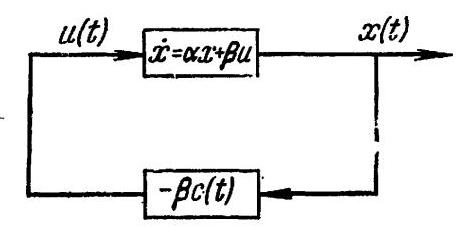
\includegraphics[max width=0.4\textwidth]{images/bo_d547k8bef24c73bgfcg0_25_951_1006_463_228_0.jpg}
\end{center}
\hspace*{3em} 

Рис. 1.5. Схема синтеза опти:- мального управления: \(u\left( t\right)  = \; =  - {\beta c}\left( t\right) x\) .

Как будет показано в главе 3, суще- ствует целый класс задач, которые могут быть решены рассмотренным методом, а именно, задачи, в которых показатель качества является квадратичной функ- цией от выхода х и управления и, а основной процесс является линейным.

Пример 5. Классический вариационный подход. В этом при- мере мы рассмотрим задачу оптимального управления с точки зрения классического вариационного исчисления. Поскольку за- висимость выходного сигнала системы x(t) от управления и (i) оп- ределяется при помощи дифференциальных уравнений динамиче- ской системы, то наша вариационная задача сводится к достаточно сложной задаче Майера—Больца. Мы рассматриваем здесь эту задачу, не останавливаясь на вопросах непрерывности и диффе- ренцируемости, и используем классические обозначения вариацион- ного исчисления.

Рассмотрим процесс управления в пространстве R", т. е. будем считать \(x\) вещественным n-мерным вектором, подчиненным урав. нению

(5)
\[
x = f\left( {x,u}\right) ,\;x\left( 0\right)  = {x}_{0}
\]

с управлениями \(u\left( t\right)  \subset  {R}^{m}\) при \(0 \leq  t \leq  1\) . Для каждого управле- ния \(u\left( t\right)\) существует соответствующий выходной сигнал \(x\left( t\right)\) , при- чем \(x\left( 0\right)\) совпадает с заданным начальным значением х, пусть также задан показатель качества

\[
C\left( u\right)  = {\int }_{0}^{1}h\left( {x,u}\right) {dt}
\]

На \(u\left( t\right)\) и x(1) не наложены никакие ограничения. Пусть и*(t) — оптимальное управление, минимизирующее \(C\left( u\right)\) , a \({x}^{ * }\left( t\right)\) — соответ- ствующий оптимальный выходной сигнал. (Векторные и матричные обозначения, используемые ниже, объяснены в приложении.)

Пусть

\[
u\left( {t,\varepsilon }\right)  = {u}^{ * }\left( t\right)  + {\varepsilon \delta u}\left( t\right)
\]

— однопараметрическое семейство управлений, полученных возму- щением в би (t) оптимального управления и*(t); каждому из них соответствует выходной сигнал

\[
x\left( {t,\varepsilon }\right)  = {x}^{ * }\left( t\right)  + {\varepsilon \delta x}\left( t\right)  + o\left( \varepsilon \right) ,\;{\delta x}\left( 0\right)  = 0.
\]

3aMethM, 4ТО

丨

\[
u\left( {t,0}\right)  = {u}^{ * }\left( t\right) ,\;\frac{\partial u}{\partial \varepsilon }\left( {t,0}\right)  = {\delta u}\left( t\right) ,
\]

\[
x\left( {t,0}\right)  = {x}^{ * }\left( t\right) ,\;\frac{\partial x}{\partial \varepsilon }\left( {t,0}\right)  = {\delta x}\left( t\right) .
\]

Рассмотрим вариацию показателя качества:

\[
{\left. \frac{\partial C}{\partial \varepsilon }\right| }_{\varepsilon  = 0} = {\delta C} = {\int }_{0}^{1}\left\lbrack  {\frac{\partial h\left( t\right) }{\partial x}{\delta x}\left( t\right)  + \frac{\partial h\left( t\right) }{\partial u}{\delta u}\left( t\right) }\right\rbrack  {dt}.
\]

Здесь \(\frac{\partial h\left( t\right) }{\partial x}\) обозначает \(\frac{\partial h\left( t\right) }{\partial x}\left( {{x}^{ * }\left( t\right) ,{u}^{ * }\left( t\right) }\right)\) . Bce другие аналогичные функции также вычисляются при \(x = {x}^{ * }\left( t\right) ,u = {u}^{ * }\left( t\right)\) . Так как минимум \(C\left( {u\left( {\cdot ,\varepsilon }\right) }\right)\) достигается при 8 = 0, то должно выполняться условие

\[
{\delta C} \equiv  0
\]

для всевозможных вариаций δu (t). Расшифруем это необходимое условие оптимального управления.

Вариация би (t) приводит к вариации \({\delta x}\left( t\right)\) , удовлетворяющей следующему дифференциальному уравнению в вариациях:

\[
\delta \dot{x} = \frac{\partial f\left( t\right) }{\partial x}{\delta x} + \frac{\partial f\left( t\right) }{\partial u}{\delta u},\;{\delta x}\left( 0\right)  = 0.
\]

Orciona

\[
{\delta x}\left( t\right)  = {\int }_{0}^{t}\Phi \left( t\right) {\Phi }^{-1}\left( s\right) \frac{\partial f\left( s\right) }{\partial u}{\delta u}\left( s\right) {ds},
\]

где фундаментальная матрица Ф(б) удовлетворяет соотношениям

\[
\dot{\Phi } = \frac{\partial f\left( t\right) }{\partial x}\Phi \;\text{ и }\;\Phi \left( 0\right)  = I.
\]

Noatomy

\[
{\delta C} = \mathop{\int }\limits_{0}^{1}\left\lbrack  {\frac{\partial h\left( t\right) }{\partial x}{\int }_{0}^{t}\Phi \left( t\right) {\Phi }^{-1}\left( s\right) \frac{\partial f\left( s\right) }{\partial u}{\delta u}\left( s\right) {ds} + \frac{\partial h\left( t\right) }{\partial u}{\delta u}\left( t\right) }\right\rbrack  {dt}.
\]

Для упрощения записн введем векторную функцию

\[
{\eta }^{ * }\left( t\right)  =  - {\eta }_{0}{\Phi }^{-1}\left( t\right)  + {\int }_{0}^{t}\frac{\partial h\left( s\right) }{\partial x}\Phi \left( s\right) {\Phi }^{-1}\left( t\right) {ds},
\]

где постоянный вектор \({\eta }_{0}\) выбран так,чтобы

\[
{\eta }^{ * }\left( 1\right)  =  - {\eta }_{0}{\Phi }^{-1}\left( 1\right)  + {\int }_{0}^{1}\frac{\partial h\left( s\right) }{\partial x}\Phi \left( s\right) {\Phi }^{-1}\left( 1\right) {ds} = 0.
\]

Это означает, что т’+ является единственным решением сопря- женного дифференциального уравнения

\[
\dot{\eta } =  - \eta \frac{\partial f}{\partial x} + \frac{\partial h}{\partial x},\;\eta \left( 1\right)  = 0.
\]

Далее, введем функцию Гамильтона, зависящую от 2n+m дей. ствительных переменных:

\[
H\left( {\eta ,x,u}\right)  = {\eta f}\left( {x,u}\right)  - h\left( {x,u}\right) .
\]

Тогда уравнения для хи ηмогут быть записаны в виде

\[
\dot{\eta } =  - \frac{\partial H}{\partial x},\;\eta \left( 1\right)  = 0
\]

H

\[
x = \frac{\partial H}{\partial x},\;x\left( 0\right)  = {x}_{0};
\]

они удовлетворяются при \(\eta  = {\eta }^{ * }\left( t\right) ,x = {x}^{ * }\left( t\right) ,u = {u}^{ * }\left( t\right)\) .

Применим теперь введенные нами обозначения для выяснения смысла необходимого условия δC ≡0. Прежде всего интегриро- ванием по частям легко проверить, что

\[
{\int }_{0}^{1}\frac{\partial h\left( t\right) }{\partial x}\Phi \left( t\right) \left( {{\int }_{0}^{t}{\Phi }^{-1}\left( s\right) \frac{\partial f\left( s\right) }{\partial u}{\delta u}\left( s\right) {ds}}\right) {dt} =
\]

\[
= \left( {{\int }_{0}^{1}\frac{\partial h\left( t\right) }{\partial x}\Phi \left( t\right) {dt}}\right) \left( {{\int }_{0}^{1}{\Phi }^{-1}\left( s\right) \frac{\partial f\left( s\right) }{\partial u}{\delta u}\left( s\right) {ds}}\right)  -
\]

\[
- {\int }_{0}^{1}\left( {{\int }_{0}^{t}\frac{\partial h\left( s\right) }{\partial x}\Phi \left( s\right) {ds}}\right) {\Phi }^{-1}\left( t\right) \frac{\partial f\left( t\right) }{\partial u}{\delta u}\left( t\right) {dt}.
\]

Используя это равенство, представим величину δC в виде

\[
{\delta C} = \left( {{\int }_{0}^{1}\frac{\partial h\left( t\right) }{\partial x}\Phi \left( t\right) {dt}}\right) \left( {{\int }_{0}^{1}{\Phi }^{-1}\left( s\right) \frac{\partial f\left( s\right) }{\partial u}{\delta u}\left( s\right) {ds}}\right)  -
\]

\[
- {\int }_{0}^{1}\left\lbrack  {\left( {{\int }_{0}^{t}\frac{\partial h\left( s\right) }{\partial x}\Phi \left( s\right) {ds}}\right) {\Phi }^{-1}\left( t\right) \frac{\partial f\left( t\right) }{\partial u} - \frac{\partial h\left( t\right) }{\partial u}}\right\rbrack  {\delta u}\left( t\right) {dt}.
\]

Но отсюда следует, что

\[
{\delta C} = {\int }_{0}^{1}\left\lbrack  {\left( {{\eta }^{ * }\left( 1\right) \Phi \left( 1\right)  + {\eta }_{0}}\right) {\Phi }^{-1}\left( t\right) \frac{\partial f\left( t\right) }{\partial u} - }\right.
\]

\[
\left. {-{\int }_{0}^{t}\left( {\frac{\partial h\left( s\right) }{\partial x}\Phi \left( s\right) {\Phi }^{-1}\left( t\right) {ds}}\right) \frac{\partial f\left( t\right) }{\partial u} + \frac{\partial h\left( t\right) }{\partial u}}\right\rbrack  {\delta udt},
\]

HJIM

丨

\[
{\delta C} = {\int }_{0}^{1}\left\lbrack  {-{\eta }^{ * }\frac{\partial f\left( t\right) }{\partial u} + \frac{\partial h\left( t\right) }{\partial u}}\right\rbrack  {\delta u}\left( t\right) {dt}.
\]

B силу того, что

\[
{\delta C} \equiv  0
\]

для всевозможных вариаций δu (t) оптимального управления \({u}^{ * }\left( t\right)\) , находим, что

\[
- {\eta }^{ * }\left( t\right) \frac{\partial f\left( t\right) }{\partial u} + \frac{\partial h\left( t\right) }{\partial u} = 0
\]

HJIM

\[
\frac{\partial H}{\partial u}\left( {{\eta }^{ * }\left( t\right) ,{x}^{ * }\left( t\right) ,{u}^{ * }\left( t\right) }\right)  \equiv  0.
\]

Более детальное исследование вариаций оптимального управления \({u}^{ * }\left( t\right)\) показывает, что \(u = {u}^{ * }\left( t\right)\) не просто критическая точка функ- ции \(H\left( {{\eta }^{ * }\left( t\right) ,{x}^{ * }\left( t\right) ,u}\right)\) , a именно максимум. Таким образом,

\[
H\left( {{\eta }^{ * }\left( t\right) ,{x}^{ * }\left( t\right) ,{u}^{ * }\left( t\right) }\right)  = \mathop{\max }\limits_{{u \in  {R}^{m}}}H\left( {{\eta }^{ * }\left( t\right) ,{x}^{ * }\left( t\right) ,u}\right) .
\]

Это и есть принцип максимума, играющий столь важную роль в теории оптимального управления. Система уравнений

\[
\dot{x} = \frac{\partial H}{\partial \eta },\;\dot{\eta } =  - \frac{\partial H}{\partial x},\;\frac{\partial H}{\partial u} = 0
\]

является системой уравнений Эйлера — Лагранжа рассматриваемой вариационной задачи (в гамильтоновой форме). В классической литературе, где отсутствуют ограничения на управление, эти усло- вия обычно называются необходимыми условиями Вейерштрасса

для экстремалей. Для пояснения рассмотрим случай, когда про- цесс описывается скалярным уравнением

\[
\dot{x} = u, : x\left( 0\right)  = {x}_{0},\;x\left( T\right)  = x,
\]

а показатель качества—функционалом

\[
C\left( u\right)  = {\int }_{0}^{T}h\left( {x,u}\right) {dt} = {\int }_{0}^{T}h\left( {x,\dot{x}}\right) {dt}.
\]

Здесь функцией Лагранжа является \(h\left( {x,\dot{x}}\right)\) и необходимое усло- вие Лагранжа для минимизирующей гладкой кривой \({x}^{ * }\left( t\right)\) есть

\[
\frac{d}{dt}\left( \frac{\partial h}{\partial \dot{x}}\right)  - \frac{\partial h}{\partial x} = 0.
\]

Полагая \(H = {\eta u} - h\) ,имеем

\[
\frac{d}{dt}\left\lbrack  {\eta  - \frac{\partial H}{\partial u}}\right\rbrack   + \frac{\partial H}{\partial x} = 0.
\]

Так kak \(\frac{\partial H}{\partial u} = 0\) , to

\[
\dot{\eta } =  - \frac{\partial H}{\partial x}.
\]

Функции η*(t) называются множителями Лагранжа вариационной задачи (в классических трудах обычно их обозначают через λ (t)). Функция Гамильтона И (п, х, и) часто берется с противоположным знаком, но мы предпочитаем принятые здесь обозначения, так как они чаще употребляются в современной литературе по оптималь- ному управлению.

Если управление и(t) ограничено по величине, или задана концевая точка \(x\left( 1\right)\) , то вариационный метод исследования услож- няется как в теоретическом, так и в вычислительном аспектах. По этой причине мы откажемся от классического вариационного подхода и будем опираться на геометрические соображения, без- укоризненные, впрочем, с точки зрения математической строгости.

\section*{Упражнения}

1. Рассмотрите управляемый процесс, описываемый уравнением х-н бхе и с ограничением |u (t)|≤1. Здесь b-действительная постоянная. Проверьте, что решение \(x\left( i\right) ,x\left( 0\right)  = {x}_{0}\) , соответствующее управлению \(u\left( t\right)\) ,имеет вид

\[
x\left( t\right)  = {e}^{-{bt}}{x}_{0} + {e}^{-{bt}}{\int }_{0}^{t}{e}^{-{bs}}u\left( s\right) {ds}.
\]

а) Покажите, что при b ≥0 можно из каждой начальной точки х, достиг- нуть начала координат \({x}_{1} = 0\) .

b) При b < 0 определите множество начальных точек, из которых можно достигнуть начала координат.

2. Рассмотрите управляемый процесс

\[
\dot{x} + {bx} = u,
\]

где b-действительная постоянная, а |u (t)|<|. Пусть хо-начальное со- стояние, из которого можно перейти в состояние х1=0. Покажите, что опти- мальное по быстродействию управление имеет вид

\[
{u}^{ * } =  - \operatorname{sgn}x.
\]

Вычислите минимальное время t* в зависимости от х, и b.

3. Рассмотрите управляемый процесс

\[
\ddot{x} + {2b}\dot{x} = u,
\]

где b—действительная постоянная, отличная от нуля и | и( t) | < 1. Покажите, что замена переменных \(x = z/{b}^{2}\) и \(t = \tau /\left| b\right|\) сводит общую задачу к одному из двух случаев \({2b} =  + 1\) и 2b=-1. Покажите, что оптимальным по быстродей- ствию управлением,переводящим \(\left( {{x}_{0},{y}_{0}}\right)\) в \(\left( {0,0}\right)\) ,будет и * \({\eta }_{2}\left( t\right)\) имеет не больше одного нуля. Постройте кривую переключения и опи- шите оптимальное управление и оптимальное решение с помощью этой кривой и с помощью экстремальных систем, для которых и (t) = +1 и и (t)=-1. При этом нужно установить различие между случаями, когда 2b=+1 и \({2b} =  - 1\) .

4. Рассмотрите управляемый процесс

\[
\ddot{x} + {2b}\dot{x} + {k}^{2}x = u,
\]

где b и \({k}^{2}\) —действительные постоянные, а мои можните, что с помощью соответствующей замены переменных эту задачу можно свести к случаю \({k}^{2} = 1,c = 1\) .

5. За какое кратчайшее время пассажир может приехать из Нью-Йорка в Лос-Анжелес? Предполагается, что в его распоряжении имеется летатель- ный аппарат с наилучшими механическими и термодинамическими свойствами, но максимальное ускорение не должно превышать 30 м/сека". (Летательный аппарат стартует в Нью-Йорке и приземляется в Лос-Анжелесе. Путь счи- тается прямолинейным длиной 3640 км. Влияние вращения и кривизны Земли можно не учитывать.)

6. Рассмотрите управляемый процесс

\[
\ddot{x} + x = u
\]

при условии |u(t)|<1. Пусть начальное состояние (х, уо) лежит выше кри- вой переключения у = W (х) управления, оптимального по быстродействию и приводящего х в начало координат. Пусть l-целое положительное число, такое, что

\[
{2l} - 1 < {\left\lbrack  {\left( {x}_{0} + 1\right) }^{2} + {y}_{0}^{2}\right\rbrack  }^{1/2} < {2l} + 1.
\]

Покажите, что оптимальное управление имеет в точности I переключений. Cформулируйте соответствующее утверждение для случая \({y}_{0} < W\left( {x}_{0}\right)\) .

7. Рассмотрите систему

\[
\dot{x} = {\alpha x} + {\beta u},
\]

аналогичную рассмотренной в примере 4. Однако показатель качества пусть будет несколько иным, а именно:

\[
C\left( u\right)  = {\int }_{0}^{T}\left( {\alpha {x}^{2} + {e}^{u}}\right) {dt}
\]

Используя метод динамического программирования, получите дифференциаль- ное уравнение в частных производных для функции \(V\left( {x,t}\right)\) .

\section*{1.2. Постановка общей задачи оптимального управления}

Наиболее общая из рассматриваемых здесь задач оптимального управления включает в себя следующие исходные данные: (1) опи- сание объекта управления, (2) начальное состояние физической системы и цель управления, (3) класс допустимых управлений, (4) показатель или критерий качества —функционал, который дает количественную оценку эффективности управления.

Прежде чем обратиться к точной формулировке задачи, обсу- дим подробно каждый из этих факторов.

1. Объект управления описывается системой обыкновенных дифференциальных уравнений

(F)
\[
\mathcal{S}){\dot{x}}^{i} = {f}^{i}\left( {t,{x}^{1},{x}^{2},\ldots ,{x}^{n},{u}^{1},\ldots ,{u}^{m}}\right) ,\;i = 1,2,\ldots ,n,
\]

связывающей вектор \(x\left( t\right)\) , xapaктеризующий состояние объекта, с входным сигналом, или управлением, и (t). Для краткости си- стему уравнений \$, описывающую объект управления, мы иногда будем называть процессом управления. Часто вектор \(x\left( t\right)\) называют выходным сигналом, однако ниже мы определим выходной сигнал как функцию от \(x\) , удовлетворяющую некоторому условию наблю- даемости. В зависимости от вида системы \$ процесс будет авто- номным, линейным, n-го порядка и т. п. (см. приложения к этой главе).

Различные нелинейные зависимости могут наблюдаться даже в простейших физических процессах вследствие нелинейного тре- ния, нелинейного усиления, насыщения. Но даже и в линейных системах при синтезе оптимальных управлений мы будем умыш- ленно вводить нелинейную обратную связь, например, типа релей- ного управления. Более того, многие физические системы содержат существенные нелинейности, которыми нельзя пренебречь и с ко- торыми не удается справиться при помощи линейной аппроксимации или применяя метод возмущений. (Рассмотренные ниже два при- мера описывают подобные существенно нелинейные системы.) В силу этого мы мало пользуемся классическим аппаратом линейной теории управления, например, интегральными преобразованиями и пере- даточными функциями.

Смысл каждой задачи оптимального управления — синтезировать управление с помощью соответствующим образом построенной цепи обратной связи. Преимущества такого замкнутого контура по сравнению с разомкнутой цепью управления заключаются в том, что процесс становится самонастраивающимся и самокорректирую- щимся. Управление с обратной связью дает возможность умень- шить влияние непредсказуемых изменений внешней среды на объект и влияние возмущений или неточности описания самого процесса.

Пример 1. Рассмотрим демпфированный нелинейный осцил- лятор с одной степенью свободы \(x\left( t\right)\) и с управлением и (t), опи. сываемый дифференциальным уравнением

\[
\ddot{x} + f\left( {x,\dot{x}}\right) \dot{x} + g\left( x\right)  = u\left( t\right) ;
\]

коэффициент трения \(f\left( {x,x}\right)  \in  {C}^{1}\left( {R}^{2}\right)\) , ynpyraя восстанавливающая сила \(g\left( x\right)  \in  {C}^{1}\left( {R}^{1}\right)\) , ynpавляющая сила и (t) ограничена и измерима на \(0 \leq  t < \infty\) . Из физической природы системы естественны пред- положения

\(f\left( {x,y}\right)  \geq  0,\;{xg}\left( x\right)  \geq  0,\;\left| {u\left( t\right) }\right|  \leq  B\) для некоторой постоянной

\[
B > 0\text{ . }
\]

Покажем сначала, что решение \(S\left( t\right)  = \left( {x\left( t\right) ,y\left( t\right) }\right)\) системы диффе- ренциальных уравнений

\[
\dot{x} = y,\;\dot{y} =  - g\left( x\right)  - f\left( {x,y}\right) y + u\left( t\right)
\]

с начальными условиями \(x\left( 0\right)  = {x}_{0},y\left( 0\right)  = {y}_{0}\) определено в фазовой плоскости \({R}^{2}\) для всех 0 ≤ t < ∞.

Действительно, если бы \(S\left( t\right)\) было определено лишь на неко- тором наибольшем промежутке времени 0≤ \(t < {\tau }_{ + } < \infty\) ,то функция \({r}^{2}\left( t\right)  = {x}^{2}\left( t\right)  + {y}^{2}\left( t\right)\) при \(t \rightarrow  {\tau }_{ + }\) должна была бы принимать сколь угодно большие значения"). Докажем, что это не так. Введем функцию, определяющуо энергию снстемы:

\[
V\left( {x,y}\right)  = \frac{{y}^{2}}{2} + {\int }_{0}^{x}g\left( s\right) {ds}.
\]

3аметим, что \(V\left( {x,y}\right)  \geq  0\) на \({R}^{2}\) и \(V = 0\) лишь на том отрезке оси х, содержащем начало координат, где g(x)=0. Положим \(V\left( t\right)  = V\left( {x\left( t\right) ,y\left( t\right) }\right)\) . Тогда

\[
\frac{dV}{dt} = y\dot{y} + g\left( x\right) \dot{x} =  - f\left( {x,y}\right) {y}^{2} + {yu}\left( t\right) .
\]

Далее,в силу элементарных неравенств

\[
\frac{dV}{dt} \leq  B\left| y\right|  \leq  B\left( {\frac{{y}^{2}}{2} + 1}\right)
\]

H

\[
\frac{d}{dt}\left\lbrack  {V\left( t\right)  + 1}\right\rbrack   \leq  B\left\lbrack  {V\left( t\right)  + 1}\right\rbrack
\]

Из последнего неравенства вытекает, что

\[
V\left( t\right)  + 1 \leq  \left\lbrack  {V\left( 0\right)  + 1}\right\rbrack  {e}^{Bt}
\]

следовательно,

\[
V\left( t\right)  \leq  \left\lbrack  {V\left( 0\right)  + 1}\right\rbrack  {e}^{B\tau } +
\]

\HRule

1) В противном случае решение \(S\left( t\right)\) можно было бы в силу теоремы о существовании решения продолжить на более широкий интервал. (Прим. ред.)

\HRule

На \(0 \leq  t < {\tau }_{ + }\) . Так KaK \(G\left( x\right)  = {\int }_{0}^{x}g\left( s\right) {ds} \geq  0\) , to

\[
{y}^{2} \leq  2\left\lbrack  {V\left( 0\right)  + 1}\right\rbrack  {e}^{B\tau } +  = {C}^{2},
\]

т. е.

\(\left| {y\left( t\right) }\right|  \leq  C\) для некоторой постоянной C.

Так как

\[
x\left( t\right)  = {x}_{0} + {\int }_{0}^{t}y\left( s\right) {ds}
\]

ТО

\[
\left| {x\left( t\right) }\right|  \leq  {x}_{0} + C{\tau }_{ + }.
\]

Но отсюда следует, что функция \(V\left( t\right)\) orраничена на конечном интервале О ≤ t < τ\_ Поэтому решение (S (t) определено при \(0 \leq  t <  + \infty\) .

Мы покажем теперь, что для каждого начального состояния \(\left( {{x}_{0},{y}_{0}}\right)  \in  {R}^{2}\) при \(t = 0\) можно выбрать такое управление \(u\left( t\right)\) , удовлетворяющее ограничению \(\left| {u\left( t\right) }\right|  \leq  B\) ,что соответствующее решение, начинаясь из точки (х, у, у), приходит в произвольно выбранную окрестность начала координат. В следующем разделе этой главы будет обсуждаться вопрос о возможности приведения фазовой точки точно в начало координат за конечное время.

Для любой постоянной \({V}_{0} \geq  0\) рассмотрим в фазовой плоскости кривую

\[
V\left( {x,y}\right)  = \frac{{y}^{2}}{2} + G\left( x\right)  = {V}_{0}.
\]

Эта кривая имеет две ветви

\[
y =  \pm  \sqrt{2\left( {{V}_{0} - G\left( x\right) }\right) }
\]

с общей точкой при \(G\left( x\right)  = {V}_{0}\) . Таким образом, эта кривая может состоять из двух отдельных ветвей; она может представлять собой замкнутую кривую, обходящую начало координат, или возможно кривую вида - или ⊂ в фазовой плоскости.

Рассмотрим свободный осциллятор, т. е. положим и (t) ≡0, и заметим, что поскольку \(x = y\) , то решение \(x\left( t\right)\) будет возрастаю- щим при у > 0 и убывающим при у < 0. Кроме того, поскольку на оси Ox \(y =  - g\left( x\right)\) , то у будет неотрицательным при хео, \(y = 0\) и неположительным при \(x \geq  0,y = 0\) . Возьмем теперь малый диск D с центром в начале координат и докажем, что решение \(S\left( t\right)  = \left( {x\left( t\right) ,y\left( t\right) }\right)\) может быть приведено в \(D\) за конечное время с помощью подходящего управления (см. рис. 1.6). Мы рассматри- ваем тот случай, когда g(x)≠0 при x≠0, т. е. когда начало координат является единственной особой точкой. Если имеется более чем одна особая точка, то малым управлением и (t) можно предотвратить остановку системы во всех других особых точках, кроме начала координат.

Сначала рассмотрим случай, когда точка (х, у, о) лежит во вто- ром квадранте; \({x}_{0} < 0,{y}_{0} > 0.\Pi\) оложим \(u\left( t\right)  = 0\) и будем следо- вать вдоль траектории \(S\left( t\right)\) до тех пор, пока не попадем либо в диск D, либо в первый квадрант. Одна из этих возможностей должна осуществиться, так как к(t) возрастает при \(y > 0\) , a тра- ектория \(S\left( t\right)\) не может достичь отрицательной полуоси и [где \(y =  - g\left( x\right)  > 0\rbrack\) и не может уйти в бесконечность, ибо она должна лежать в области

\[
V\left( {x,y}\right)  \leq  V\left( {{x}_{0},{y}_{0}}\right) ,\;\text{ поскольку }\;\dot{V} =  - f\left( {x,y}\right) {y}^{2} \leq  0.
\]

Если точка \(\left( {{x}_{0},{y}_{0}}\right)\) лежит в первом квадранте или траектория \(S\left( t\right)\) попадает в первый квадрант при возрастании \(t\) ,то полагаем \(u\left( t\right)  =  - B < 0\) . Тогда \(y \leq   - B\) и траектория \(S\left( t\right)\) должна пере- сечь положительную полуось и и попасть в четвертый квадрант. B четвертом квадранте мы положим \(u\left( t\right)  = 0\) и тогда траектория \(S\left( t\right)\) попадет либо в D либо в третий квадрант. В третьем квад- ранте положим \(u\left( t\right)  = B\) .

Таким образом, с помощью описанного выше управления мы заставляем траекторию \(S\left( t\right)\) закручиваться по спирали (по часо- вой стрелке) вокруг начала координат. Поскольку

\[
\dot{V} =  - f\left( {x,y}\right) {y}^{2} + {yu}\left( t\right)  \leq  0
\]

(н V) \(< 0\) при \(y \neq  0\) ),то нетрудно видеть,что

\[
\mathop{\lim }\limits_{{t \rightarrow   + \infty }}V\left( t\right)  = 0
\]

Однако область \(V\left( {x,y}\right)  < \varepsilon\) для достаточно малых \(\varepsilon  > 0\) пересе- кается с D так, что спираль \(S\left( t\right)\) непременно войдет в D. Cледо- вательно, фазовая точка может быть приведена в произвольную малую окрестность начала координат.

П р име p 2. Рассмотрим твердое тело, например, космический корабль, вращающийся в инерциальном пространстве вокруг своего центра тяжести с угловой скоростью ω (t) под действием управляю- щего момента u (t). Пусть \({\omega }_{1},{\omega }_{2},{\omega }_{3}\) — проекции мгновенной угловой скорости о (t) на оси координат, совпадающие с главными осями инерции тела В. Тогда уравнения Эйлера движения твердого тела в фазовом пространстве \({R}^{3}\) переменных \(\left( {{\omega }_{1},{\omega }_{2},{\omega }_{3}}\right)\) имеют такой

вид:

\[
{I}_{1}{\dot{\omega }}_{1} = \left( {{I}_{2} - {I}_{3}}\right) {\omega }_{2}{\omega }_{3} + {u}_{1}\left( t\right) ,
\]

\[
{I}_{2}{\dot{\omega }}_{2} = \left( {{I}_{3} - {I}_{1}}\right) {\omega }_{3}{\omega }_{1} + {u}_{2}\left( t\right) ,
\]

\[
{I}_{3}{\dot{\omega }}_{3} = \left( {{I}_{1} - {I}_{2}}\right) {\omega }_{1}{\omega }_{2} + {u}_{3}\left( t\right) .
\]

Здесь \({I}_{1},{I}_{2},{I}_{3} -\) главные моменты инерции твердого тела отно- сительно соответствующих осей, а \({u}_{1},{u}_{2},{u}_{3}\) —проекции и (t) на те же оси. Предположим, что управляющий момент создается находящимися на корабле реактивными двигателями, максималь- ная тяга которых не зависит от характера движения корабля B, т. е.

\[
\left| {{u}_{i}\left( t\right) }\right|  \leq  1,\;i = 1,2,3.
\]

Наша цель — регулировать вектор угловой скорости \(\omega \left( t\right)\) так, чтобы он приближался к нулю. В следующем разделе мы рас- смотрим вопрос о существовании управления и (t), приводящего 10 (t) в точности к нулю за ко- нечное время.

\begin{center}
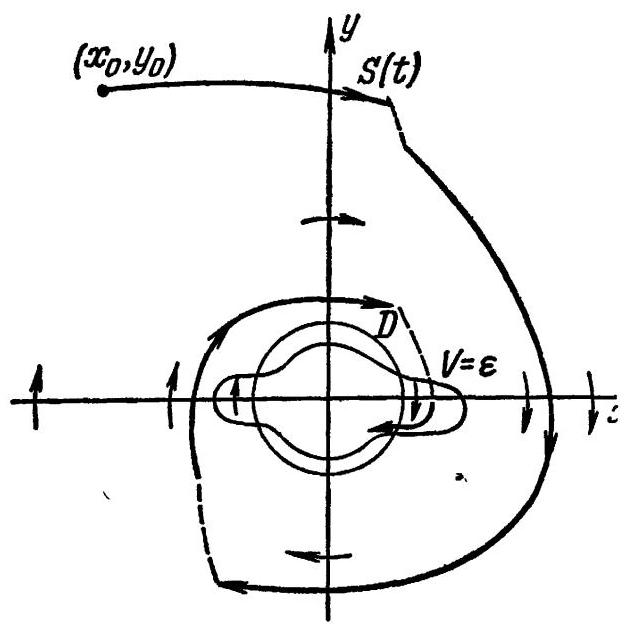
\includegraphics[max width=0.5\textwidth]{images/bo_d547k8bef24c73bgfcg0_35_803_799_629_629_0.jpg}
\end{center}
\hspace*{3em} 

Рис. 1.6. Управляемость нелинейной си- стемы x+f (x, x) x+g (x) =u (t).

Определим кинетическую энергию системы

\[
E = \frac{1}{2}\left( {{I}_{1}{\omega }_{1}^{2} + {I}_{2}{\omega }_{2}^{2} + {I}_{3}{\omega }_{3}^{2}}\right)
\]

и вычислим производную Ё вдоль любого решения ω (t):

\[
\dot{E} = {I}_{1}{\omega }_{1}{\dot{\omega }}_{1} + {I}_{2}{\omega }_{2}{\dot{\omega }}_{2} + {I}_{3}{\omega }_{3}{\dot{\omega }}_{3} =
\]

\[
= {\omega }_{1}{u}_{1} + {\omega }_{2}{u}_{2} + {\omega }_{3}{u}_{3}.
\]

Положим \({u}_{i} =  - \frac{1}{2}\alpha {I}_{i}{\omega }_{i} \; \left( {i = 1,2,3}\right)\) ; если α—достаточно малая положительная постоянная, то \(\left| {u}_{i}\right|  \leq  1\left( {i = 1,2,3}\right)\) вдоль всей траектории ω (t), соответствующей управлению u \(= \left( {{u}_{1},{u}_{2},{u}_{3}}\right)\) . Кроме того, при выбранном управлении \(\dot{E} =  - {\alpha E}\) , так что с воз- растанием t величина E экспоненциально убывает. Поэтому \(\lim \omega \left( t\right)  = 0\) и в сколь угодно малую окрестность начала коорди- нат можно попасть за конечное время.

2. Начальная точка или состояние хотя это заданный в фазо- вом пространстве вектор. В реальном физическом процессе ком- поненты вектора \({x}_{0}\) и вектора \(x\left( t\right)\) могут представлять собой положение, скорости, угловые скорости, температуру и другие параметры, измеряемые и регистрируемые соответствующими при- борами (см. обсуждение вопроса о наблюдаемости в гл. 2 и 6).

В задаче управления заранее определяется также и цель управ- ления, которая состоит в приведении объекта в заданное состоя- ние \({x}_{1}\) или,в более общем случае,в заданное множество конечных состояний G, называемое целевым множеством.

Иногда целевое множество будет представлять собой непре- рывно зависящее от \(t\left( {{\tau }_{0} \leq  t \leq  {\tau }_{1}}\right)\) компактное множество \(G{\left( t\right) }^{-1}\) ). Это означает, что для каждого момента времени и из данного интервала задается непустое компактное множество \(G\left( t\right)\) в фазо- вом пространстве \({R}^{n}\) . Непрерывность \(G\left( t\right)\) как функции действи тельной переменной \(t\) определяется с помощью понятия расстояния между \(G\left( t\right)\) и \(G\left( {t}^{\prime }\right)\) , вводимого следующим образом:

\(\operatorname{dist}\left( {G\left( t\right) ,G\left( {t}^{\prime }\right) }\right)  = \max \left\lbrack  {\mathop{\max }\limits_{{P \in  G\left( t\right) }}\operatorname{dist}\left( {P,G\left( {t}^{\prime }\right) }\right) ,\mathop{\max }\limits_{{{P}^{\prime } \in  G\left( {t}^{\prime }\right) }}\operatorname{dist}\left( {{P}^{\prime },G\left( t\right) }\right) }\right\rbrack  .\)

Таким образом, для любого t и заданного ε> 0 найдется такое \(\delta  > 0\) ,что dist \(\left( {G\left( t\right) ,G\left( {t}^{\prime }\right) }\right)  < \varepsilon\) ,как только \(\left| {{t}^{\prime } - t}\right|  < \delta\) . Если \(G\left( t\right)\) есть точка, непрерывно движущаяся по гладкой кривой ξ (t) в R", то часто приходится рассматривать ошибку, или отклонение \(x\left( t\right)\) от желаемого положения:

\[
e\left( t\right)  = x\left( t\right)  - \xi \left( t\right) .
\]

Здесь под \(x\left( t\right)\) понимается выходной сигнал управляемого про- цесса

(F)
\[
\dot{x} = f\left( {t,x,u}\right) ,
\]

а процессуправления величиной \(e\left( t\right)\) опнсывается уравнением

\[
\dot{e} = f\left( {t,e + \xi \left( t\right) ,u}\right)  - \dot{\xi }\left( t\right)  = \widetilde{f}\left( {t,e,u}\right) .
\]

В такой интерпретации целью управления является сведение ошибки \(e\left( t\right)\) к нулю.

3. Класс ∆ допустимых управлений обычно состоит из изме- римых функций \(u\left( t\right)\) на различных интервалах времени б, причем каждое из этих управлений переводит объект из начальной точки \({x}_{0}\) в одну из точек заданного целевого множества G (t), т. e. решение \(x\left( t\right)\) уравнения

(\$)
\[
\dot{x} = f\left( {t,x,u}\right) ,\;x\left( {t}_{0}\right)  = {x}_{0}
\]

должно удовлетворять условию \(x\left( {t}_{1}\right)  \in  G\left( {t}_{1}\right)\) .

Предположим, что S автономная система, и точка х, перево- дится в точку \({x}_{1}\) управлением \({u}_{1}\left( t\right)\) на интервале \({t}_{0} \leq  t \leq  {t}_{1}\) . Если управление \({u}_{2}\left( t\right)\) на интервале \({t}_{0} \leq  t \leq  {t}_{2}\) переводит точку \({x}_{1}\) в точку \({x}_{2}\) , то результирующее управление

\[
u\left( t\right)  = \left\{  \begin{array}{ll} {u}_{1}\left( t\right) , & {t}_{0} \leq  t \leq  {t}_{1}, \\  {u}_{2}\left( {t - {t}_{1} + {t}_{0}}\right) , & {t}_{1} \leq  t \leq  {t}_{1} + {t}_{2} - {t}_{0} \end{array}\right.
\]

\HRule

1) Так обстоит дело в том случае, когда цель управления зависит от момента времени, в который заканчивается управление. (Прим. ред.)

\HRule

переводит \({x}_{0}\) в \({x}_{2}\) . Поэтому нетрудно показать, что, не ограничи- вая общности, всегда можно считать началом управления t=0.

Часто на функции из класса, А накладываются различные дополнительные ограничения; например, условие и (t) ⊂Ω, где \(\Omega\) —фиксированное компактное выпуклое множество в R", назы- ваемое ограничивающим множеством \({}^{1}\) ). Кроме того, иногда за- дается заранее начало и конец интервала времени, в течение которого происходит управление.

4. Критерий, или показатель качества представляет собой принятый количественный критерий эффективности каждого уп- равления \(u\left( t\right)\) на интервале t, с t с t, из класса Δ. Если дро- стоит из управлений, определенных на различных интервалах времени и приводящих х, в целевое множество, то критерий ка. чества управления и (t) часто определяется следующим образом:

\[
C\left( u\right)  = {\int }_{{t}_{0}}^{{t}_{1}}{f}^{0}\left( {t,x\left( t\right) ,u\left( t\right) }\right) {dt},
\]

где \({f}^{0}\left( {t,x,u}\right)\) -заданная непрерывная функция. Если \({f}^{0}\left( {t,x,u}\right)  \equiv  1\) , ro \(C\left( u\right)  = {t}_{1} - {t}_{0}\) ,и мы получаем задачу оптималь- ного быстродействия.

Иногда ∆ состоит из управлений, действующих на фиксиро- ванном промежутке времени, например, \({t}_{0} \leq  t \leq  T\) , or которых требуется лишь приближенное приведение системы в положение \(\xi \left( t\right)\) . Тогда критерий качества часто бывает таким:

\[
C\left( u\right)  = \left| {x\left( T\right)  - \xi \left( T\right) }\right|  + {\int }_{{t}_{0}}^{T}{f}^{0}\left( {t,x\left( t\right) ,u\left( t\right) }\right) {dt}.
\]

В частности, весьма распространены квадратичные критерии качества, включающие среднюю ошибку управляемого движения \(x\left( t\right)\) и энергию, pacxoдуемую при управлении \(u\left( t\right)\) ,т. e.

\[
C\left( u\right)  = g\left( {x\left( T\right) }\right)  + {\int }_{{t}_{0}}^{T}\left\lbrack  {{x}^{\prime }\left( t\right) {W}_{u}^{\prime }\left( t\right) x\left( t\right)  + {u}^{\prime }\left( t\right) U\left( t\right) u\left( t\right) }\right\rbrack  {dt}.
\]

Здесь g(x)—неотрицательная функция, а W (t), U (t)—симметрич- ные положительно определенные (полуопределенные) матрипы, т. е. \({x}^{\prime }{Wx} > 0\left( { \geq  0}\right)\) и \({u}^{\prime }{Uu} > 0\) [для любых ненулевых век- торов \(x,u\) .

\HRule

1) B opermnade crestraint sets. (Прим. ред.)

\HRule

Задача оптимального быстродействия для линейных систем рассматривается в главе 2, а квадратичный критерий качества изучается в главе 3.

Теперь рассмотрим задачу управления, включающую в себя: (1) процесс \$, (2) начальное положение х, и целевое множество \(G\left( t\right) ,\left( 3\right)\) класс допустимых управлений \(\Delta\) и (4) критерий качества \(C\left( u\right)\) , который определен для всех управлений и из непустого множества ∆.

Определение. Управление и*(t) из класса ∆ называется олмциальным по опиошению к кригерию качесгия

\[
C\left( {u}^{ * }\right)  \leq  C\left( u\right)
\]

для всех и (t) \(\in  \Delta\) .

В главах 2 и 3 будет доказано существование оптимального управления для линейных систем с различными критериями ка- чества. В главе 4 мы докажем довольно общие теоремы сущест- вования оптимальных управлений для нелинейных систем; в качестве примера приведем формулировку одной из таких теорем.

Теорема 1. Пусть поставлена задача управления, т. е. за- даны:

1) Система дифференциальных уравнений

\[
\text{ (C) }{\dot{x}}^{i} = {g}^{i}\left( {t,x}\right)  + {h}_{j}^{i}\left( {t,x}\right) {u}^{j}\;\left( {i = 1,\ldots ,n,j = 1,\ldots ,m}\right) \text{ , }
\]

cãe

\[
{g}^{i}\left( {t,x}\right) ,{h}_{j}^{i}\left( {t,x}\right) \text{ и }\frac{\partial {g}^{i}\left( {t,x}\right) }{\partial {x}^{k}},\frac{\partial {h}_{j}^{i}\left( {t,x}\right) }{\partial {x}^{k}}\;\left( {k = 1,\ldots ,n}\right)
\]

— непрерывные на \({R}^{1} \times  {R}^{n}\) функции;

2) непустое выпуклое компактное ограничивающее множество \(\Omega  \subset  {R}^{m}\)

3) начальное положение \({x}_{0} \in  {R}^{n}\) и непрерывно зависящее от \(t\left( {{\tau }_{0} \leq  t \leq  {\tau }_{1}}\right)\) компактное целевое множество \(G\left( t\right)  \subset  {R}^{n}\) ;

4) критерий качества

\[
C\left( u\right)  = {\int }_{{t}_{0}}^{{t}_{1}}\left\lbrack  {{g}^{0}\left( {t,x\left( t\right) }\right)  + {h}_{j}^{0}\left( {t,x\left( t\right) }\right) {u}^{j}\left( t\right) }\right\rbrack  {dt},
\]

где дв (н. х) и hi (1, к) — непрерывные на R1 × R’ функции.

Пусть Δ = Δ(\$, Ω, х, G) — класс измеримых управлений \(u\left( t\right)  \subset  \Omega\) на подынтервалах \({t}_{0} \leq  t \leq  {t}_{1}\) интервала то : t < 0 реводящих \(x\left( {t}_{0}\right)  = {x}_{0}\) в \(x\left( {t}_{1}\right)  \in  G\left( {t}_{1}\right)\) .

Предположим, что:

(a) \(\Delta  -\) непустое множество;

(b) существует такое \(B < \infty\) ,что \(\left| {x\left( t\right) }\right|  \leq  B\) для всех упра ляемых движений x(t), соответствующих управлениям из Δ.

Тогда в классе ∆ существует оптимальное управление и* (t).

Можно также доказать, что если класс \(\Delta \left( \alpha \right)  \subset  \Delta\) , cocтоящий из допустимых управлений с фиксированным начальным моментом времени \({t}_{0} = \alpha\) непуст, то в нем существует оптимальное управ- ление [это верно и для подкласса ∆ (α, β) ⊂ Δ управлений с фик- сированными начальным и конечным моментами].

Доказательство этой и других теорем существования, а также примеры систем, не обладающих оптимальными управлениями, будут приведены в главе 4. Все доказательства существования основаны на использовании следующих трех фактов: (1) Δ\_He- пустое множество, (2) множество ∆ слабо компактно, так что cy- шествует предел и*(t) для подходящей последовательности управ- лений \({u}_{k}\left( t\right)\) ,на которых значения функционала C(u) убывают, (3) функционал \(C\left( u\right)\) обладает свойством непрерывности, так что \(\lim C\left( {u}_{n}\right)  = C\left( {u}^{ * }\right)\) . K сожалению, все эти теоремы существования \(n \rightarrow  \infty\) не конструктивны. Поэтому для построения оптимального управ- ления требуется дальнейшее исследование.

Для случая линейного управляемого процесса

\[
\dot{x} = A\left( t\right) x + B\left( t\right) u
\]

с интегрируемыми коэффициентами легко видеть, что предполо- жение (b) сформулированной выше теоремы выполняется автома- тически. В следующем разделе мы рассмотрим предположение (а), которое связано с понятием управляемости.

\section*{1.3. Основные результаты теории управляемости}

B этом разделе мы обсудим возможность перевода системы из начального состояния \({x}_{0}\) в точности в заданное состояние \({x}_{1}\) за конечный промежуток времени.

Определение. Автономный процесс управления

\[
\dot{{x}^{i}} = {f}^{i}\left( {{x}^{1},\ldots ,{x}^{n},{u}^{1},\ldots ,{u}^{m}}\right) \;\left( {i = 1,\ldots ,n}\right) ,
\]

где \(f\left( {x,u}\right)  \in  {C}^{1}\) на \({R}^{n} \times  {R}^{m}\) ,называется вполне управляемым,если для каждой пары точек \({x}_{0}\) и \({x}_{1}\) из \({R}^{n}\) существует ограниченное измеримое управление и(t) на некотором конечном интервале \(0 \leq  t \leq  {t}_{1}\) , Такое,что соответствующее движение \(x\left( t\right)\) переводит систему из точки \(x\left( 0\right)  = {x}_{0}\) в точку \(x\left( {t}_{1}\right)  = {x}_{1}\) .

Замечание. Для неавтономного процесса

\[
\dot{x} = f\left( {t,x,u}\right)
\]

понятие управляемости изменяется следующим образом: для каж- дого начального момента времени б, процесс считается управляе- мым, если для любого начального положения \({x}_{0}\) и любого конеч- ного положения \({x}_{1}\) cyществует такое ограниченное измеримое управление \(u\left( t\right)\) на интервале \({t}_{0} \leq  t \leq  {t}_{1}\) ,что соответствующее движение \(x\left( t\right)\) переводит систему из точки \(x\left( {t}_{0}\right)  = {x}_{0}\) в точку \(x\left( {t}_{1}\right)  = {x}_{1}\) .

В главе 2 мы докажем следующую теорему об управляемости линейных систем:

Теорема 2. Линейный процесс

\[
\dot{x} = {Ax} + {Bu},
\]

где А—действительная постоянная (п×п)-матрица, В—действи- тельная постоянная (п×т)-матрица, является вполне управляемым тогда и только тогда, когда ранг (n×nm)-матрицы

\[
\left\lbrack  {B,{AB},{A}^{2}B,\ldots ,{A}^{n - 1}B}\right\rbrack
\]

равен n.

B примерах, приведенных в разделе 1.2, рассматривалась задача приведения системы в начало координат. Были указаны случаи, когда из любого начального положения можно было привести систему в некоторую окрестность начала координат. Ниже мы покажем, какое управление следует применить, чтобы попасть в точности в начало координат.

Определение. Для процесса

\[
{\dot{x}}^{i} = {f}^{i}\left( {{x}^{1},\ldots ,{x}^{n},{u}^{1},\ldots ,{u}^{m}}\right) ,\;i = 1,\ldots ,n,
\]

где \(f\left( {x,u}\right)  \in  {C}^{1}\) на \({R}^{n} \times  {R}^{m}\) , oбластью нуль-управляемости \(\mathfrak{C}\) назы- вается множество всех точек \({x}_{0} \in  {R}^{n}\) ,из которых система может быть переведена в начало координат с помощью допустимого управления \(u\left( t\right)\) за конечный промежуток времени 0≤ \(t \leq  {t}_{1}\) .

В главе 6 мы докажем следующую основную теорему о при- ведении системы в точку покоя.

Теорема 3. Рассмотрим процесс

\[
{\dot{x}}^{i} = {f}^{i}\left( {{x}^{1},\ldots ,{x}^{n},{u}^{1},\ldots ,{u}^{m}}\right) ,\;i = 1,\ldots ,n,
\]

где f(x, u) \(\in  {C}^{1}\) на \({R}^{n} \times  {R}^{m}\) .

Предположим, что:

(a)
\[
f\left( {0,0}\right)  = 0;
\]

(b) класс \(\Delta\) допустимых управлений включает все измеримые управления и (t), которые определены на конечных интервалах вре- мени и удовлетворяют условию | и (t)|≤ε для некоторого ε>0;

(c) система линейных дифференциальных уравнений

\[
\dot{x} = {Ax} + {Bu}
\]

спос𝚖оянными мапричами коэффициенмов

\[
A = \left( {\frac{\partial {f}^{i}}{\partial {x}^{j}}\left( {0,0}\right) }\right) \text{ и }B = \left( {\frac{\partial {f}^{j}}{\partial {u}^{k}}\left( {0,0}\right) }\right)
\]

управляема, т. е.

\[
\operatorname{rank}\left\lbrack  {B,{AB},{A}^{2}B,\ldots ,{A}^{n - 1}B}\right\rbrack   = n\text{ . }
\]

Тогда область € нуль-управляемости содержит некоторую откры- тую окрестность начала координат в R".

Чтобы показать, насколько сильна эта теорема, отметим одно ее прямое следствие, которое в главе 2 будет доказано незави- симо от теоремы 3.

Следствие. Рассмотрим линейную систему управления

\[
\dot{x} = {Ax} + {Bu},
\]

где А—действительная постоянная п×п-матрица, В—действи- тельная постоянная п×т-матрица.

Предположим, что

a) Матрица А устойчива, т. е. все ее собственные значения \(\lambda\) удовлетворяют условию Re \(\lambda  < 0\) ;

b) выполняется условие управляемости, т. е.

\[
\operatorname{rank}\left\lbrack  {B,{AB},\ldots ,{A}^{n - 1}B}\right\rbrack   = n\text{ . }
\]

Тогда система из любой начальной точки х, может быть пе- реведена в точку х, =0 некоторым измеримым управлением и (t) на конечном интервале 0 0 ≤t ≤ t, - Более того, и (t) удовлетворя- em условию \(\left| {u\left( t\right) }\right|  \leq  \varepsilon\) для произвольного ε>0.

Приложения сформулированной выше теоремы к примерам 1 и 2 раздела 1, а также и к другим интересным специальным случаям мы предлагаем в качестве упражнений.

В оставшейся части этого раздела мы познакомимся с некото- рыми задачами управления, в которых система описывается не матричным уравнением, а одним линейным дифференциальным уравнением высокого порядка. Рассмотрим линейную систему, описываемую уравнением

\[
{x}^{\left( n\right) } + {a}_{1}\left( t\right) {x}^{\left( n - 1\right) } + \ldots  + {a}_{n}\left( t\right) x = u\left( t\right) ,
\]

где \(u\left( t\right)\) -скалярное управление, ограниченное по величине, а именно, лежащее в некотором интервале 7. Может возникнуть задача: перевести систему из начального состояния ( \({x}_{0}\) , \({x}_{0}\) , \(\left. {{x}_{0},\ldots ,{x}_{0}^{\left( n - 1\right) }}\right)\) в желаемое состояние \(G\) ,например, \(x = 0\) ,и далее сохранять это состояние управлением из J. Задачи такого типа часто встречаются в теории одномерных и многомерных систем управления. Мы сейчас рассмотрим пример такой задачи; более подробно она будет изложена в главе 2.

Пример 1. Рассмотрим линейный управляемый процесс

\[
\dddot{x} + 2\ddot{x} + 2\dot{x} + x = u,\;\left| {u\left( t\right) }\right|  \leq  1.
\]

Предположнм, что мы хотим прнвести к нулю скорость \(\dot{x}\) н ускорение х системы, а ее смещение х для нас несущественно. Иначе говоря, пусть требуется из любого начального состояния \(\left( {{x}_{0},{\dot{x}}_{0},{\ddot{x}}_{0}}\right)\) перейти в желаемое состояние хе 0, х=0 и в даль- нейшем сохранять нулевые значения скорости и ускорения, ис- пользуя управление и (t), удовлетворяющее условию [и(t)] \(\leq  1\) . Эту задачу можно записать и в виде системы трех дифференци- альных уравнений первого порядка

\[
{\dot{x}}^{1} = {x}^{2},\;{\dot{x}}^{2} = {x}^{3},\;{\dot{x}}^{3} =  - {x}^{1} - 2{x}^{2} - 2{x}^{3} + u\left( t\right) ,
\]

вводя новые переменные \({x}^{1},{x}^{2},{x}^{3}\) . Целевое множество G будет представлять собой прямую \({x}^{2} = 0,{x}^{3} = 0\) в \({R}^{3}\) . Мы будем называть ядром множества G и обозначать символом core (G) совокупность всех точек из G, обладающих следующим свойством: для каждой точки \({x}_{0} \in  \operatorname{core}\left( G\right)\) cyществует такое управление \(u\left( t\right)\) на интервале \(0 \leq  t < \infty\) c orpaничением \(\left| {u\left( t\right) }\right|  \leq  1\) ,что соответствующее реше- ние \(x\left( t\right) ,x\left( 0\right)  = {x}_{0}\) не покидает множества G,т. е. \({x}^{2}\left( t\right)  = {x}^{3}\left( t\right)  = 0\) при \(0 \leq  t < \infty\) . Но тогда \({x}^{2}\left( t\right)  = {\dot{x}}^{3}\left( t\right)  = 0\) и,следовательно,

\[
{x}^{1}\left( t\right)  = u\left( t\right) \;\text{ и }\;\left| {x}^{1}\right|  \leq  1.
\]

C другой стороны, любая начальная точка вида (и, 0, 0), где \(\left| {x}_{0}^{1}\right|  \leq  1\) ,может быть навсегда задержана в \(G\) , если восполь- зоваться постоянным управлением и (t) = х, таким образом,

\[
\operatorname{core}\left( G\right)  = \left\{  {\left| {x}^{1}\right|  \leq  1,{x}^{2} = 0,{x}^{3} = 0}\right\}  ,
\]

т. e. core \(\left( G\right)\) есть cermetн ocu \({x}^{1}\) .

Итак, задача, состоящая в том, чтобы привести систему в G и удерживать ее затем там, полностью совпадает с задачей при- ведения системы в ядро множества G. Следовательно, мы свели задачу приведения системы в G с дополнительным условием ее дальнейшего удерживания в G к более стандартной задаче при- ведения системы в новую цель — core (G) без дополнительных усло- вий. Отметим, что целевое множество системы core \(\left( G\right)\) является компактным выпуклым множеством в R³.

Интересно, что управление, приводящее систему с последую- щим удерживанием в плоскость

\[
{G}^{\prime } = \left\{  {{x}^{2} = 0}\right\}  ,
\]

налагаетна решение условие \(\dot{{x}^{2}} = \dot{{x}^{3}} = 0\) ; такнм образом,

\[
\operatorname{core}\left( {G}^{\prime }\right)  = \operatorname{core}\left( G\right)
\]

Поэтому первоначальная задача двумерного управления, приво- дящего систему в \(G = \left\{  {{x}^{2} = 0,{x}^{3} = 0}\right\}\) ,может быть заменена одно- мерной задачей приведения в область \({G}^{\prime } = \left\{  {{x}^{2} = 0}\right\}\) . Этот факт является иллюстрацией одного общего результата, который будет получен в дальнейшем.

Другой тип линейных задач теории управления, в которых появляются производные управляющей функции, можно назвать задачей с дифференциальным оператором управления. У линейных систем такого вида передаточная функция является дробно-рацио- нальной функцией, числитель которой определяется управляющей функцией и ее производными. Природа таких задач становится ясной из следующего ниже примера. Подробнее они будут изу- чены в главе 2.

Пример 2. Рассмотрим линейную задачу с дифференциаль- ным оператором управления

(L)
\[
\ddot{x} + 3\dot{x} + {2x} = 2\dot{u} + u,
\]

где управление \(u\left( t\right)\) класса \({C}^{1}\) подчинено ограничению \(\left| {u\left( t\right) }\right|  \leq  1\) . Передаточная функция для разомкнутого контура имеет вид

\[
\frac{{2p} + 1}{{p}^{2} + {3p} + 2}
\]

Отметим, что числитель 2p+1 определяется видом правой части \(2\dot{u} + u\) .

Пусть требуется перевести систему из начального состояния \(\left( {{x}_{0},{\dot{x}}_{0}}\right)\) в точку (0,0) за минимальное возможное время. Чтобы записать эту задачу с помощью системы линейных уравнений в фазовом пространстве, положим х=у. Тогда получим следую- IIIYIO CHCTEMY:

\[
\dot{x} = y,\;\dot{y} =  - {2x} - {3y} + 2\dot{u} + u.
\]

В дальнейшем будет показано, что в классе \({C}^{1}\) не существует оптимального управления для этой системы; поэтому требуется расширить класс допустимых управлений, включив в него раз- рывные функции. Для этого запишем нашу задачу (Z) в виде линейной системы несколько иного вида (см. главу 2, упражне- ние 4.5):

(5)
\[
{\dot{x}}^{1} = {x}^{2} + {2u},\;{\dot{x}}^{2} =  - 2{x}^{1} - 3{x}^{2} - {5u}.
\]

Передаточная функция системы (\$) вычисляется следующим об- разом:

\[
p\overline{{x}^{1}} = \overline{{x}^{2}} + 2\bar{u},\;p\overline{{x}^{2}} =  - 2\overline{{x}^{1}} - 3\overline{{x}^{2}} - 5\overline{u},
\]

где \({\bar{x}}^{1},{\bar{x}}^{2},\bar{u}\) -соответствующие преобразования Лапласа. Таким образом,

\[
{\bar{x}}^{1} = \frac{{2p} + 1}{{p}^{2} + {3p} + 2}\bar{u}.
\]

Заметим, что система \$ не содержит производных от и и поэтому к ней можно применять обычную методику теории управления, предложенную в главе 2. Следует также отметить, что фазовые координаты х, \(y = x\) теперь входят в следующем виде:

\[
{x}^{1} = x,\;{x}^{2} = y - {2u},
\]

а начальное состояние \({x}^{1}\left( 0\right)  = {x}_{0},{x}^{2}\left( 0\right)  = {x}_{0} - {2u}\left( 0\right)\) зависит от управления \(u\left( t\right)\) . Эту трудность, однако, можно обойти, исполь- зуя управления, у которых и (0) = 0, или же заменяя начальную точку начальным (cerментом \({x}^{1} = {x}_{0},{y}_{0} - 2 \leq  {x}^{2} \leq  {y}_{0} + 2\) . Кроме того, можно вовсе не рассматривать систему ( \(\mathcal{L}\) ), а считать си- стему \$ исходным описанием нашей задачи с заданным началь- ным состоянием ( \({x}_{0}^{1},{x}_{0}^{2}\) ).

Действительно, на практике эквивалентная система £ часто имеет удовлетворительную физическую трактовку, а уравнение 𝒳, содержащее дифференциальный оператор управления, выводится из системы \$ с помощью дифференцирования и последующего исключения неизвестных —операций, которые при применении к системе с разрывным управлением не являются, строго говоря, допустимыми.

\section*{1.4. Экстремальные свойства оптимальных управлений и их синтез}

В дифференциальном исчислении для нахождении минимума функции действительного переменного требуется провести иссле- дование критических точек, т. е. точек, в которых производная функции обращается в нуль. Аналогичной процедуре мы следуем в теории оптимального управления.

В этом разделе мы сформулируем принцип максимума, смысл которого заключается в том, что каждое оптимальное управление является максимальным, т. е. «критическим» для заданной задачи управления. Мы рассматриваем здесь лишь автономные системы; более общий случай неавтономных систем будет подробно изучен в главе 5. Рассмотрим задачу автономного управления, в описа- ние которой входят:

1. Cистема ( \(f){x}^{i} = {f}^{i}\left( {{x}^{1},\ldots ,{x}^{n},{u}^{1},\ldots ,{u}^{m}}\right) ,i = 1,2\ldots ,n\) , где \(f\left( {x,u}\right)  \in  {C}^{1}\) в \({R}^{n} \times  \Omega\) .

2. Начальное состояние \({x}_{0}\) и целевое множество G-непустое компактное подмножество в R \textdegree .

3. Класс Δ, включающий все измеримые управления и (t), определенные на различных конечных промежутках времени \(0 \leq  t \leq  {t}_{1}\) ,переводящие точку \({x}_{0}\) в \(G\) и принадлежащие некото- рому непустому компактному ограничивающему подмножеству Ω в \({R}^{m}\) .

4. Критерий качества \(C\left( u\right)  = {\int }_{0}^{{t}_{1}}{f}^{0}\left( {x\left( t\right) ,u\left( t\right) }\right) {dt}\) ,где \({f}^{0}\left( {x,y}\right)  \in  {C}^{1}\) в \({R}^{n} \times  \Omega\) .

Определение. Рассмотрим автономный управляемый про- цесс \(\{ \widehat{\mathcal{S}},{x}_{0},G,\Omega ,\Delta ,C\}\) , onисанный выше. Пусть \(u\left( t\right) ,\left( {0 \leq  t \leq  {t}_{1}}\right)  -\) некоторое управление из \(\Delta\) , которому соответствует решение \(\mathbf{x}\left( t\right)  = \left( {{x}^{i}\left( t\right) }\right) ,\;i = 1,\ldots ,n\) . Рассмотрим вместо вектора \(\mathbf{x}\left( t\right) \; n + 1\) -мерный вектор

\[
\widehat{\mathbf{x}}\left( t\right)  = \left( {{x}^{\alpha }\left( t\right) }\right) ,\;\alpha  = 0,1,\ldots ,n,
\]

где

\[
{x}^{0}\left( t\right)  = {\int }_{0}^{t}{f}^{0}\left( {x\left( t\right) ,u\left( t\right) }\right) {dt}.
\]

\(n + 1\) -мерный вектор \(\widehat{\mathbf{\eta }}\left( t\right)  = \left( {{\eta }_{\alpha }\left( t\right) }\right) ,0 \leq  t \leq  {t}_{1}\) называется сопря- женным решением для \(\widehat{x}\left( t\right)\) , если \(\widehat{\eta }\left( t\right)\) есть решение гамильтоно- вой системы

\[
{\dot{x}}^{\alpha } = \frac{\partial \widehat{H}}{\partial {\eta }_{\alpha }} = {f}^{\alpha }\left( {x,u\left( t\right) }\right) ,\;\alpha  = 0,1,\ldots ,n,
\]

\[
{\dot{\eta }}_{\alpha } =  - \frac{\partial \widehat{H}}{\partial {x}^{\alpha }} =  - {\eta }_{0}\frac{\partial {f}^{0}}{\partial {x}^{\alpha }}\left( {x,u\left( t\right) }\right)  - \ldots  - {\eta }_{n}\frac{\partial {f}^{n}}{\partial {x}^{\alpha }}\left( {x,u\left( t\right) }\right) ,
\]

не обращающееся в нуль ни в какой точке отрезка 0≤ < t <.t. Здесь функция Гамильтона имеет вид

\[
\widehat{H}\left( {\widehat{\eta },\widehat{x},u}\right)  = {\eta }_{0}{f}^{0}\left( {x,u}\right)  + {\eta }_{1}{f}^{1}\left( {x,u}\right)  + \ldots  + {\eta }_{n}{f}^{n}\left( {x,u}\right) .
\]

Положим

\[
\widehat{M}\left( {\widehat{\eta },\widehat{x}}\right)  = \mathop{\max }\limits_{{u \in  \Omega }}\widehat{H}\left( {\widehat{\eta },\widehat{x},u}\right) .
\]

Тогда, по определению, управление \(u\left( t\right) ,0 \leq  t \leq  {t}_{1}\) ,будет макси- мальным, если существует решение \(\eta \left( t\right)\) ,такое,что

1. \(\widehat{H}\left( {\widehat{\eta }\left( t\right) ,\widehat{x}\left( t\right) ,u\left( t\right) }\right)  = \widehat{M}\left( {\eta \left( t\right) ,\widehat{x}\left( t\right) }\right)\) почти всюду на \(0 \leq  t \leq  {t}_{1}\) .

2. \(\widehat{M}\left( {\widehat{\eta }\left( t\right) ,\widehat{x}\left( t\right) }\right)  = 0\) всюду на отрезке [0, \({t}_{1}\rbrack ;{\eta }_{0} \leq  0\) .

Следующая теорема называется принципом максимума для автономных систем.

Теорема 4. Рассмотрим управляемую автономную систему \(\left( {\mathcal{S},{x}_{0},\bar{G},\Omega ,\Delta ,C}\right)\) , onucaнную выше. Пусть и (t), \(0 \leq  t \leq  {t}_{1}\) ,— оптимальное управление из класса ∆. Тогда и (t) является макси- мальным управлением.

Заметим, что и (t) называется максимальным управлением, хотя оно доставляет минимум функционалу С (и). Чтобы не из- менять традиционные термины, принятые в литературе по управ- лению, мы будем мириться с этим несоответствием.

Для пояснения природы принципа максимума применим его к следующей линейной задаче:

1. \(S : x = {Ax} + {Bu}\) , \(\Gamma\) дe \(A\) и \(B\) —действительные постоянные \(\left( {n \times  n}\right)\) - и \(\left( {n \times  m}\right)\) -матрицы соответственно.

2. Начальное положение \({x}_{0}\) принадлежит области нуль-управ- ляемости, а целевое множество G есть начало координат.

3. Ограничивающее множество Ω есть компактное выпуклое подмножество в \({R}^{m}\) .

4. Критерием качества является продолжительность процесса управления:

\[
C\left( u\right)  = {\int }_{0}^{{t}_{1}}{dt} = {t}_{1}
\]

В этом случае функция Гамильтона имеет такой вид:

\[
\widehat{H}\left( {\widehat{\eta },\widehat{x},u}\right)  = {\eta }_{0} + \eta \left\lbrack  {{Ax} + {Bu}}\right\rbrack   = {\eta }_{0} + H\left( {\eta ,x,u}\right) ,
\]

где \(\eta  = \left( {\eta }_{i}\right) ,i = 1,\ldots ,n, - n\) -мерный вектор-строка и \(\eta \left\lbrack  {{Ax} + {Bu}}\right\rbrack   = H\) . Тогда

\[
\widehat{M}\left( {\widehat{\eta },\widehat{x}}\right)  = {\eta }_{0} + {\eta Ax} + \mathop{\max }\limits_{{u \in  \Omega }}{\eta Bu} = {\eta }_{0} + M\left( {\eta ,x}\right) ,
\]

где \(M = \max H\) . Econ \(u\left( t\right) ,0 \leq  t \leq  {t}_{1}, - \max\) симальное управление, то решение \(x\left( t\right)  = \left( {{x}^{i}\left( t\right) }\right) ,i = 1,\ldots ,n\) , a также сопряженное ре- шение \(\eta \left( t\right)  = \left( {{\eta }_{i}\left( t\right) }\right) ,i = 1,\ldots ,n\) yдовлетворяют уравнениям

\[
\dot{x} = {Ax} + {Bu}\left( t\right) ,\;\dot{\eta } =  - {\eta A};
\]

при этом \({x}^{0} = t,{\eta }_{0} =\) const.

Принцип максимума означает, во-первых, что

\[
{\eta }_{0} + \eta \left( t\right) {Ax}\left( t\right)  + \eta \left( t\right) {Bu}\left( t\right)  = {\eta }_{0} + \eta \left( t\right) {Ax}\left( t\right)  + \mathop{\max }\limits_{{u \in  \Omega }}\eta \left( t\right) {Bu}
\]

ИЛИ

\[
\eta \left( t\right) {Bu}\left( t\right)  = \mathop{\max }\limits_{{u \in  \Omega }}\eta \left( t\right) {Bu}
\]

почти всюду на интервале \(0 \leq  t \leq  {t}_{1}\) и,во-вторых,что

\[
{\eta }_{0} + \eta \left( t\right) {Ax}\left( t\right)  + \mathop{\max }\limits_{{u \in  \Omega }}\eta \left( t\right) {Bu} = 0
\]

всюду на отрезке [0, t,]. Если вектор-функция \(\eta \left( t\right)\) обращается в нуль в какой-либо одной точке интервала 0≤<t<t, то она тождественно равна нулю на \(\left\lbrack  {0,{t}_{1}}\right\rbrack\) ,так как является решением однородной линейной системы

\[
\dot{\eta } =  - {\eta A}.
\]

Но если и \(\left( t\right)  \equiv  0\) ,то \({\eta }_{0} = 0\) ,что противоречит определенню век- тора дем (н). Следовательно, вектор-функция \(\eta \left( t\right)\) не обращается в нуль ни в одной точке интервала 0≤ \(t \leq  {t}_{1}\) .

Таким образом, в этом случае можно не рассматривать до- полнительные компоненты \({x}^{0} = t\) и \({\eta }_{0} =\) const,т. e. перейти к \(n\) -мерным векторам \(x\left( t\right)\) и \(\eta \left( t\right)\) и искать максимальное управ- ление \(u\left( t\right)\) в зависимости от \(H\left( {\eta ,x,u}\right)\) и \(M\left( {\eta ,x}\right)\) . Heo6xo- димо отметить, что сопряженное решение удовлетворяет вполне определенной системе дифференциальных уравнений

\[
\dot{\eta } =  - {\eta A},
\]

коэффициенты которой не зависят от управления и (t) и решения х (t). Таким образом, η (t) полностью определяется начальными усло- виями. Так как условия принципа максимума однородны, т. е. допускают умножение η (t) на любую положительную постоянную, то это можно учесть при выборе начальных условий.

Рассмотрим важный частный случай, когда для описанной выше линейной автономной управляемой системы Ω представляет со- бой m-мерный куб \(\left| {u}^{j}\right|  \leq  1\) . Тогда условие

\[
\eta \left( t\right) {Bu}\left( t\right)  = \mathop{\max }\limits_{{u \in  \Omega }}\eta \left( t\right) {Bu}
\]

означает, что каждая компонента управления и(t) может быть выбрана равной либо +1, либо —1 в зависимости от знака соот- ветствующей компоненты вектора η(t) В. Таким образом, макси- мальное управление и (t) удовлетворяет равенству

\[
u\left( t\right)  = {\left\lbrack  \operatorname{sgn}\eta \left( t\right) B\right\rbrack  }^{\prime }
\]

почти всюду,если только компоненты η (t) \(B\) не обращаются в нуль на подмножестве положительной меры из интервала 0≤<мск. Заметим, что это есть как раз то самое условие экстремальности оптимального управления, которое было выведено в примерах раздела 1.1 из геометрических соображений, связанных со свой- CTBOM выпуклости множества достижимости.

Теперь мы можем попытаться синтезировать максимальное управление

\[
u\left( t\right)  = {\left\lbrack  \operatorname{sgn}\eta \left( t\right) B\right\rbrack  }^{\prime },
\]

определив сначала сопряженное решение η (t), а затем проинтег- рировав уравнение

\[
\dot{x} = {Ax} + B{\left\lbrack  \operatorname{sgn}\eta \left( t\right) B\right\rbrack  }^{\prime }
\]

с обратным отсчетом времени, начиная отсчет в начале координат \(x = 0\) и заканчивая его в исходной точке х, при этом мы про- буем различные начальные значения вектора η(t), например, единичный вектор при \(t = 0\) , a затем строим и (t) и х не о. Если построить таким способом все возможные максимальные управления и соответствующие им решения, то одно из них будет оптимальным управлением (если такое вообще существует), пере- водящим точку \({x}_{0}\) в начало координат. После этого мы возвраща- емся к прежнему направлению отсчета времени, сдвинув начало отсчета так, чтобы и, соответствовало не 0. Эта процедура уже использовалась нами при построении кривой переключения и син- тезировании оптимального управления в примерах раздела 1.1.

Весьма важным для синтеза максимального, а следовательно, и оптимального управления является соображение единственности. Процесс управления, обладающий свойством единственности, мы будем называть нормальным; в дальнейшем будет развита специ- альная теория нормальных процессов управления. В частности, будет показано, что задача приведения к началу координат ли- нейной автономной управляемой системы

\[
{x}^{\left( n\right) } + {a}_{1}{x}^{\left( n - 1\right) } + \ldots  + {a}_{n}x = u
\]

за минимальное возможное время при условии \(\mid  u\left( t\right)  \mid   \leq  1\) является нормальной. Таким образом, при синтезе оптимального управления как релейного управления, возможно использование принципа мак- симума, максимальных управлений, а также кривых переключения.

\section*{1.5. Синтез оптимальных управлений для линейных систем второго порядка}

В этом разделе мы закончим построение оптимального по бы- стродействию управления для линейных систем второго порядка наиболее общего вида [рассматривается задача приведения системы из точки (x, x) в начало координат).

Итак, рассмотрим систему

\[
\ddot{x} \pm  {2b}\dot{x} \pm  {k}^{2}x = u,
\]

где \(b \geq  0\) и \({k}^{2} > 0 -\) константы, a управление подчинено ограни- чению \(\left| {u\left( t\right) }\right|  \leq  1\) .

В разделе 1.1 уже рассматривался наиболее общий вид линей- ных систем первого порядка

\[
\dot{x} \pm  {bx} = u,\;\left| {u\left( t\right) }\right|  \leq  1.
\]

Исследовались также некоторые частные случаи систем второго порядка, например,

\[
\ddot{x} \pm  b\dot{x} = u,\;\left| {u\left( t\right) }\right|  \leq  1
\]

и

\[
\ddot{x} + {k}^{2}x = u,\;\left| {u\left( t\right) }\right|  \leq  1.
\]

В упражнениях было показано, что ограничение более общего вида на величину управления |u(t)|≤c, где c>0, сводится к стандартному ограничению \(\left| {u\left( t\right) }\right|  \leq  1\) соответствующим измене- нием масштаба. Рассмотренные ниже случаи развивают решение задачи синтеза оптимальных по быстродействию управлений для любых автономных линейных систем второго порядка.

Рассмотрим вопрос о синтезе оптимального по быстродействию управления в задаче о приведении к нулю линейной системы

(
\[
\mathcal{Z}
\]
 )
\[
\ddot{x} \pm  {2b}\dot{x} \pm  {k}^{2}x = u
\]

с коэффициентами \(b \geq  0\) и \({k}^{2} > 0\) и ограничением \(\left| {u\left( t\right) }\right|  \leq  1\) . За- метим, что соответствующая система уравнений

(F)
\[
\dot{\mathbf{x}} =
\left[ \begin{array}{cc}
0 & 1 \\
\pm {k}^{2} & \pm {2b}
\end{array} \right]
\mathbf{x} + \left[ \begin{array}{c}
0 \\
1
\end{array} \right] u
\]

является нормальной и управляемой. Следовательно, по теоремам разделов 1.2 и 1.3 существует единственное оптимальное управ- ление \({u}^{ * }\left( t\right)\) на интервале 0 ≤ t ≤ t*, переводящее систему из за- данного начального состояния \(\left( {{x}_{0},{y}_{0}}\right)\) ,лежащего в области нуль- управляемости \(\mathfrak{C}\), в точку (0, 0). При этом \(\mathfrak{C}\) является открытым связным множеством в фазовой плоскости \({R}^{2}\) .

В силу принципа максимума, сформулированного в разделе 1.4, оптимальное управление является максимальным, и выражается формулой

\[
{u}^{ * }\left( t\right)  = \operatorname{sgn}{\eta }_{2}\left( t\right)
\]

почти всюду на интервале 0≤ t ≤ t*. Здесь сопряженное решение \(\eta \left( t\right)  = \left( {{\eta }_{1}\left( t\right) ,{\eta }_{2}\left( t\right) }\right)\) удовлетворяет системе уравнений

\[
{\dot{\eta }}_{1} =  \pm  {k}^{2}{\eta }_{2}
\]

\[
{\dot{\eta }}_{2} =  - {\eta }_{1} \pm  {2b}{\eta }_{2}
\]

HJH

\[
{\ddot{\eta }}_{2} \mp  {2b}{\dot{\eta }}_{2} \pm  {k}^{2}{\eta }_{2} = 0.
\]

Заметим, что \({\eta }_{2}\left( t\right)\) не может быть тождественным нулем, так как в этом случае

\[
{\eta }_{1}\left( t\right)  =  \pm  {2b}{\eta }_{2}\left( t\right)  - {\dot{\eta }}_{2}\left( t\right)  = 0,
\]

что противоречит условию \(\eta \left( t\right)  \neq  0\) на \(0 \leq  t \leq  {t}^{ * }\) . B силу анали- тичности функции \({\eta }_{2}\left( t\right)\) она может иметь лишь конечное число нулей на интервале 0 ≤ \(t \leq  {t}^{ * }\) .

Вследствие нормальности системы У существует лишь одно максимальное управление, переводящее ( \({x}_{0},{y}_{0}\) ) в (0,0), а следо- вательно, и одно оптимальное управление и*(t). Мы построим соответствующую кривую переключений у =W(x), на которой происходит переключение экстремальной траектории с решения системы

\[
\left( {\mathcal{S}}_{ - }\right)
\]

\[
\dot{x} = y,\;\dot{y} =  \mp  {k}^{2}x \mp  {2by} - 1
\]

на решение системы

\[
\left( {\mathcal{S}}_{ + }\right)
\]

\[
\dot{x} = y,\;\dot{y} =  \mp  {k}^{2}x \mp  {2by} + 1,
\]

и наоборот. Так как замена переменных \(x \rightarrow   - x,y \rightarrow   - y\) пере- водит \({\mathcal{S}}_{ - }\) в \({\mathcal{S}}_{ + }\) , to ясно,что \(W\left( {-x}\right)  =  - W\left( x\right)\) ,и поэтому до- статочно искать кривую переключений лишь для \(x > 0\) .

Таким образом, синтез оптимального управления \({u}^{ * }\left( t\right)\) сводится к определению области € управляемости и построению кривой переключений \(y = W\left( x\right)\) .

Пример 1. Демпфированный линейный осциллятор. Рассмот- рим задачу о приведении в начало координат за минимальное время системы

(Y)
\[
\ddot{x} + {2b}\dot{x} + {k}^{2}x = u.
\]

Здесь \(b > 0\) и \({k}^{2} > 0\) — постоянные, и | и ( t ) | ≤ 1 . Поскольку матрица

\[
A = \left[ \begin{array}{cc} 0 & 1 \\   - {k}^{2} &  - {2b} \end{array} \right]
\]

устойчива, то в силу следствия из теоремы раздела 1.3 областью нуль-управляемости € будет все пространство R2.

Здесь имеется два качественно различных случая:

1) слабое демпфирование, \({b}^{2} - {k}^{2} < 0\) ,

2) критическое и сильное демпфирование, \({b}^{2} - {k}^{2} \geq  0\) .

Рассмотрим сначала случай b²-k² <0. Тогда каждое реше- ние экстремальной системы

\[
\left( {\mathcal{S}}_{ - }\right)
\]

\[
\left\lbrack  \begin{array}{l} \dot{x} \\  \dot{y} \end{array}\right\rbrack   = \left[ \begin{array}{cc} 0 & 1 \\   - {k}^{2} &  - {2b} \end{array} \right]   \cdot  \left\lbrack  \begin{array}{l} x \\  y \end{array}\right\rbrack   - \left\lbrack  \begin{array}{l} 0 \\  1 \end{array}\right\rbrack
\]

представляет собой спираль, закручивающуюся вокруг особой точки (положения равновесия) 0-: \(x =  - 1/{k}^{2},y = 0\) , a каждое решение системы\(\left( {\mathcal{S}}_{ + }\right)\)

\[
\left\lbrack  \begin{array}{l} \dot{x} \\  \dot{y} \end{array}\right\rbrack   = \left[ \begin{array}{cc} 0 & 1 \\   - {k}^{2} &  - {2b} \end{array} \right]  \left\lbrack  \begin{array}{l} x \\  y \end{array}\right\rbrack   + \left\lbrack  \begin{array}{l} 0 \\  1 \end{array}\right\rbrack
\]

есть спираль, закручивающаяся вокруг особой точки \({O}_{ + } : x = \frac{1}{{k}^{2}}\) , \(y = 0\) при \(t \rightarrow  \infty\) . Любая экстремальная траектория, приводящая в начало координат, должна состоять из конечного числа кусков интегральных кривых систем \({\mathcal{G}}_{ - }\) и \({\mathcal{G}}_{ + }\) с чередующимся переклю- чением. Анализ сопряженного решения \({\eta }_{2}\left( t\right)  = \alpha {e}^{bt}\sin \left( {{\omega t} + \beta }\right)\) , где α ≠ 0, β-произвольные постоянные, и ω = V /в г. показы- вает, что промежуток времени между последовательными пере- ключениями равен \(T = \pi /\omega\) .

Пусть \({S}_{ + }\) — решение системы У., которое при обратном от- счете времени исходит из начала координат (рис. 1.7). Опишем с помощью этого решения кривую переключения \(y = W\left( x\right)\) при \(x \geq  0\) , a затем докажем справедливость этого построения.

Построим кривую переключений, развертывая спираль S, в точках пересечения с осью х. Пусть \({S}_{ + }^{1}\) есть дуга траектории \({S}_{ + }\) , ведущая из точки (0, 0) в направлении, противоположном указан- ному стрелкой на рис. 1.7, к предшествующей точке пересечения траектории \({S}_{ + }\) с осью х. Очевидно, что дуга \({S}_{ + }^{1}\) и ее отражение \({S}_{ - }^{1}\) относительно начала координат являются частью кривой пере- ключения, так как каждая точка дуги представляет собой точку переключения для максимальной или экстремальной траектории решения системы \$\_, которая пересекает дугу и затем по ней приводит в начало координат.

\begin{center}
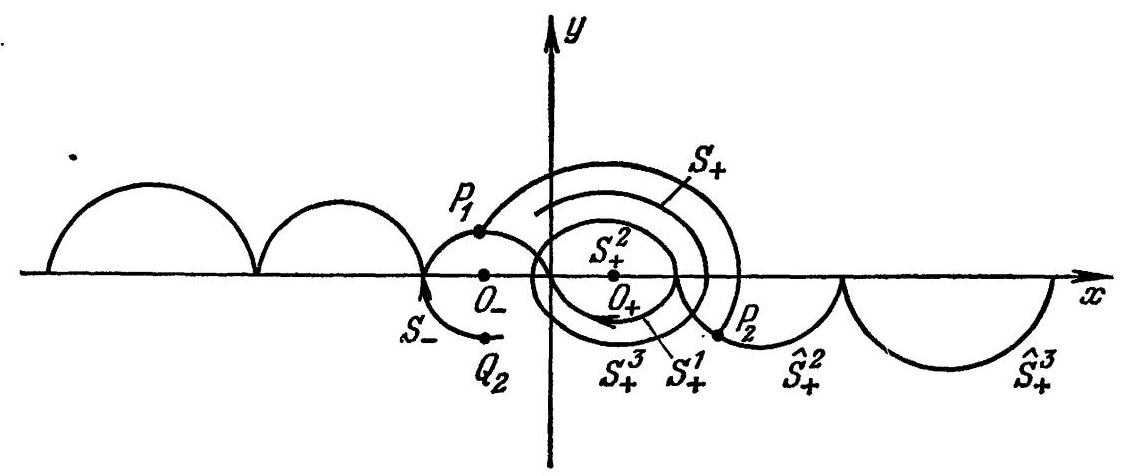
\includegraphics[max width=1.0\textwidth]{images/bo_d547k8bef24c73bgfcg0_51_218_604_1124_476_0.jpg}
\end{center}
\hspace*{3em} 

Рис. 1.7. Оптимальное по быстродействию управление, приводящее систему в начало координат. График кривой переключения для системы х-2bх+k²х=u, |u(t)|<1. Cлy Чай 1, пример 1: \({b}^{2} - {k}^{2} < 0,b > 0,{k}^{2} > 0\) .

Рассмотрим последовательные дуги спирали 8,+: \({S}_{ + }^{1},{S}_{ + }^{2},{S}_{ + }^{3},\ldots\) ; каждая из них представляет собой половину оборота спирали 8, и начинается в точке пересечения спирали с осью х. На полуоси \(x \geq  0\) кривая переключения \(y = W\left( x\right)\) строится из дуги \({S}_{ + }^{1}\) и дуг \({\widehat{S}}_{ + }^{2},{\widehat{S}}_{ + }^{3},\ldots ,\) являющихся результатом переноса дуг \({S}_{ + }^{2},{S}_{ + }^{3},\ldots\) вдоль оси х. Таким образом, мы образуем непрерывную кривую \(y = W\left( x\right)\) , odнозначную по \(x\) на положительной полуоси х≥0 и такую, что при возрастании \(x\) точки дуг \({\widehat{S}}_{ + }^{1},{\widehat{S}}_{ + }^{2},\ldots\) идут в том же порядке, что и точки дуг \({S}_{ + }^{1},{S}_{ + }^{2},\ldots\) при возрастании (— t).

Для \(x < 0\) положим \(W\left( x\right)  =  - W\left( {-x}\right)\) . Определим теперь син- тезнрующуо функцию \(\Psi \left( {x,y}\right)\) так,чтобы решения уравнения

\[
\ddot{x} + {2b}\dot{x} + {k}^{2}x = \Psi \left( {x,\dot{x}}\right)
\]

всегда давали бы оптимальные траектории, переводящие систему из любой начальной точки (х, уо) в начало координат (0, 0).

Для этого положим [для всех действительных (х, у) ≠ (0, 0)]

\[
\Psi \left( {x,y}\right)  = \begin{cases}  - 1 & \text{ для }y > W\left( x\right) \text{ ина }{S}_{ - }^{1}, \\  0 & \text{ для }y = W\left( x\right) , \\   + 1 & \text{ для }y < W\left( x\right) \text{ ина }{S}_{ + }^{1}. \end{cases}
\]

Чтобы проверить правильность нашего построения, начнем дви- жение с куска \({S}_{ + }^{1}\) решения \({\mathcal{S}}_{ + }\) системы \({\mathcal{S}}_{ + }\) и куска \({S}_{ - }^{1}\) решения \({S}_{ - }\) системы G\_. Кривая переключения вправо от \({S}_{ + }^{1}\) состоит из кусков решений системы G+, взятых на интервалах \(T = \frac{\pi }{\omega }\) и ис- ходящих из точек \({S}_{ - }^{1}\) .

Рассмотрим точку Р„=( \({x}^{1}\) , \({y}^{1}\) ) на \({S}_{ - }^{1}\) и обозначим через \({P}_{2} = \left( {{x}^{2},{y}^{2}}\right)\) точку, в которую мы придем через промежуток времени \(T = \frac{\pi }{\omega }\) ,двигаясь вдоль решения системы \$+. Тогда точки Р1, \({O}_{ + }\) и \({P}_{2}\) будут лежать на одной прямой, и отношение длин от- резков \({P}_{1}{O}_{ + }\) и \({O}_{ + }{P}_{2}\) равняется \({e}^{-{bT}}\) . Это легко вычислить, учи- тывая, что точки \({P}_{1}\) и \({P}_{2}\) лежат на одном и том же витке спи- рали S, с характеристикой затухания евги на расстоянии в пол- витка. Однако отношение длины отрезка \({Q}_{3}{O}_{ - }\) ,где \({Q}_{2} = \left( {{x}_{ - }^{2},{y}_{ - }^{2}}\right)  -\) точка траектории \({S}_{ - }\) ,лежащая на прямой \({P}_{1}{O}_{ - }\) ,к длине отрезка \({P}_{1}{O}_{ - }\) также равно еъть. Из подобия треугольников находим, что \({y}_{ - }^{2} = {y}^{2}\) , a затем простым вычислением можно показать, что \({x}^{2} = {x}_{ - }^{2} + \left( {{e}^{\frac{b\pi }{\omega }} + 1}\right) \frac{2}{{k}^{2}}\) . Это означает,что дуга \({\widehat{\mathcal{S}}}_{ + }^{2}\) , Bходящая в кри- вую переключения, представляет собой результат параллельного переноса дуги \({S}_{ - }^{2}\) , которая лежит на траектории S\_ и является продолжением дуги S1. Но дуги \({S}_{ - }^{2}\) и S+ получаются друг из друга параллельным переносом, так как системы \$\_ и \$\_ нере- ходят одна в другую при замене переменных \(\left( {x,y}\right)  \rightarrow  \left( {-x, - y}\right)\) . Таким образом, дуга \({\widehat{\mathcal{S}}}_{ + }^{2}\) является следующим за \({\mathcal{S}}_{ + }^{1}\) куском линии переключения \(y = W\left( x\right)\) при \(x > 0\) . Полное описание кривой \(y = W\left( x\right)\) получается повторением этого рассуждения.

Обратимся к случаю (2) \({b}^{2} - {k}^{2} \geq  0\) . Здесь каждое решение систем \({\mathcal{S}}_{ \pm  }\) приближается соответственно к точкам 0,…,однако на каждом решении х может обращаться в нуль не более одного раза. Общее решение сопряженного уравнения имеет вид

\[
{\eta }_{2}\left( t\right)  = {e}^{bt}\left( {\alpha  + {\beta t}}\right) \;\pi {p}_{H}\;{b}^{2} - {k}^{2} = 0
\]

HAM

\[
{\eta }_{2}\left( t\right)  = \alpha {e}^{bt}\operatorname{sh}\left( {{\mu t} + \beta }\right) \;\text{ при }\;{b}^{2} - {k}^{2} > 0,
\]

где а и β—постоянные и μ= \(\sqrt{{b}^{2} - {k}^{2}}\) . В любом случае цензи не правонос первозов имеет самое большее один нуль, а соответствующее оптимальное управление таково:

\[
{u}^{ * }\left( t\right)  = \operatorname{sgn}{\eta }_{2}\left( t\right) .
\]

В случае (2) кривая переключений у = W (х) состоит из двух кусков решений Г\_ и Г\_. Здесь Г\_ представляет собой решение системы \$\_, проходящее через точку (0, 0), а г. — решение си- стемы g\_i, лежащее в четвертом квадранте, как показано на рис. 1.8, и ведущее из начала координат. Таким образом, легко построить кри- вую переключений \(y = W\left( x\right)\) ,которая будет однозначной на всей оси х, а также соответствующую синтезирую- щую функцию

\[
\Psi \left( {x,y}\right)  = \left\{  \begin{array}{l}  - 1\text{ при }y > W\left( x\right) \text{ ина }{\Gamma }_{ - }, \\   + 1\text{ прн }y < W\left( x\right) \text{ ина }{\Gamma }_{ + }. \end{array}\right.
\]

\begin{center}
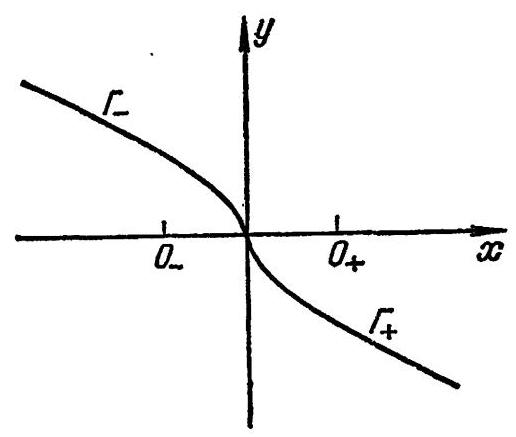
\includegraphics[max width=0.4\textwidth]{images/bo_d547k8bef24c73bgfcg0_53_882_405_516_437_0.jpg}
\end{center}
\hspace*{3em} 

Рис. 1.8. Оптимальное по быстро- действию управление, приводящее систему в начало координат. График кривой переключения для системы \(\ddot{x} + {2b}\dot{x} + {k}^{2}x = u,\left| {u\left( t\right) }\right|  \leq  1\) . C л y. qa й 2, \(\Pi\) p и м е р 1 : \({b}^{2} - {k}^{2} \geq  0\) , \(b > 0,{k}^{2} > 0\) .

Пример 2. Линейный/осцилля- тор с отрицательным трением. Pac- смотрим задачу приведения в начало координат за минимальное время си- CTEMbI

\[
\ddot{x} - {2b}\dot{x} + {k}^{2}x = u.
\]

3 десь b > 0 и \({k}^{2} > 0 -\) постоянные, a \(\left| {u\left( t\right) }\right|  \leq  1\) . Заметим,что система дифференциальных уравнений

(F)
\[
\left\lbrack  \begin{array}{l} \dot{x} \\  \dot{y} \end{array}\right\rbrack   = \left\lbrack  \begin{array}{rr} 0 & 1 \\   - {k}^{2} & {2b} \end{array}\right\rbrack  \left\lbrack  \begin{array}{l} x \\  y \end{array}\right\rbrack   + \left\lbrack  \begin{array}{l} 0 \\  1 \end{array}\right\rbrack  u
\]

не является устойчивой в начале координат (при \(u \equiv  0\) ),однако она управляема и нормальна.

Так же как и в примере 1, для построения кривой переклю- чений и синтеза оптимального управления рассмотрим экстре- мальные системы\(\left( {\mathcal{S}}_{ - }\right)\)

\[
\dot{x} = y,\;\dot{y} =  - {k}^{2}x + {2by} - 1
\]

и

\[
\left( {\mathcal{S}}_{ + }\right)
\]

\[
\dot{x} = y,\;\dot{y} =  - {k}^{2}x + {2by} + 1.
\]

Здесь снова возможны два случая:

1) слабое демпфирование, \({\dot{b}}^{2} - {k}^{2} < 0\) ,

2) критическое и сильное демпфирование, вы зна

Рассмотрим случай 1, b²-k² с 0. Здесь каждое решение си- стемы f\_ представляет собой раскручивающуюся спираль с цент- ром в точке \({O}_{ - } : x =  - \frac{1}{{k}^{2}},y = 0\) , a каждое решение системы \({\mathcal{S}}_{ + }\) - спираль с центром в точке \({O}_{ + } : x = \frac{1}{{k}^{2}},y = 0\) , packручивающуюся с возрастанием t. В наиболее общем виде сопряженную траекторию можно представить так:

\[
{\eta }_{2}\left( t\right)  = \alpha {e}^{-{bt}}\sin \left( {{\omega t} + \beta }\right) ,
\]

где \(\alpha ,\beta\) — постоянные и ω = \(\sqrt{{k}^{2} - {b}^{2}}\) . Таким образом, экстремаль- ная траектория, приводящая в точку (0, 0), может иметь много переключений между дугами \$\_ и \$\_; промежуток времени между переключениями всегда должен, однако, равняться Т = π/ω.

Кривая переключения строится методом, аналогичным употреб- лявшемуся в примере 1. Пусть \({S}_{ + }^{1}\) -дуга кривой \({S}_{ + }\left\lbrack  {S}_{ + }\right.\) pewe- ние системы \$+, исходящее из точки (0, 0)], отсчитанная от начала координат и соответствующая промежутку времени T = π/ω (при обратном отсчете времени). Пусть S+, S+ последователь- ные дуги кривой \({S}_{ + }\) , каждая из которых начинается и заканчи- вается в точке пересечения \({S}_{ + }\) с осью \(x\) и соответствует проме- жутку времени \(T = \pi /\omega\) . Тогда кривая \(y = W\left( x\right)\) будет состоять из дуги \({S}_{ + }^{1}\) ,за которой будет следовать \({S}_{ + }^{2}\) ,а затем своего рода развертка спирали, с остриями в точках пересечения кривой \({S}_{ + }\) c ocъю \(x\) (puc. 1.9).

\begin{center}
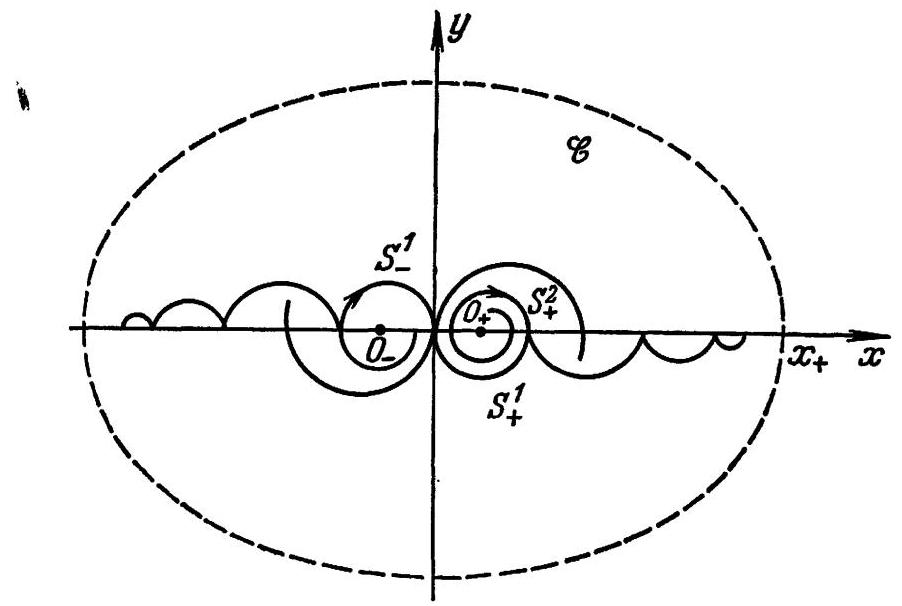
\includegraphics[max width=0.8\textwidth]{images/bo_d547k8bef24c73bgfcg0_54_322_981_902_606_0.jpg}
\end{center}
\hspace*{3em} 

Рис. 1.9. Оптимальное по быстродействию управление, приводящее систему в начало координат. График кривой переключения для системы х-2b \(x + {k}^{2}x = u.\;\left| {u\left( t\right) }\right|  < 1\) . Cлy чай 1, пример 2: \({b}^{2} - {k}^{2} < 0,b > 0,{k}^{2} > 0\) .

Поскольку диаметр дуги \({S}_{ + }^{1}\) равняется \(\left( {{e}^{-\frac{b\pi }{\omega }} + 1}\right) \frac{1}{{k}^{2}}\) , a диа- метры последующих дуг убывают, так как множитель е-блт/... с 1, то нетрудно вычислить, что у =W (х) определена для следующих 3Haчений \(x\) :

\[
0 \leq  x < {x}_{ + } = \frac{1 + {e}^{-{b\pi }/\omega }}{\left( {1 - {e}^{-{b\pi }/\omega }}\right) {k}^{2}}.
\]

Пользуясь нечетностью функции \(W\left( x\right)  =  - W\left( {-x}\right)\) ,можно доопре- делить \(W\left( x\right)\) на \({x}_{ - } < x \leq  0\) ,где \({x}_{ - } =  - {x}_{ + }\) .

Легко видеть, что область управляемости € есть открытая область, ограниченная решением \$\_, ведущим из точки (x\_, 0) в точку (x, 0) при у ≥0, и решением \$, ведущим из точки \(\left( {{x}_{ + },0}\right)\) в точку ( \({x}_{ - },0\) ) при \(y \leq  0\) . Таким образом, синтезирующая функция определяется в 6 следующим образом:

\[
\Psi \left( {x,y}\right)  = \begin{cases}  - 1\text{ для }y > W\left( x\right) \text{ и на }{S}_{ - }^{1}, \\  0\text{ для }y = W\left( x\right) , \\   + 1\text{ для }y < W\left( x\right) \text{ ина }{S}_{ + }^{1}. \end{cases}
\]

Теперь рассмотрим случай 2, b²-k² ≥0. Каждое решение систем \({\mathcal{G}}_{ \pm  }\) исходит из особой точки \({O}_{ \pm  }\) и имеет не более чем одну точку пересечения с осью х. Следовательно, каждая опти- мальная траектория, приводящая в точку \(\left( {0,0}\right)\) ,будет иметь не более одного пере- ключения. Решения системы S+ легко получить из решений \$\_ (пример 1, слу- чай 2) подстановкой \(x \rightarrow   - x,y \rightarrow  y\) , \(t \rightarrow   - t\) . Решения \$\_ аналогично полу- чаются из решений \$\_ аналогично полу- чай 2).

\begin{center}
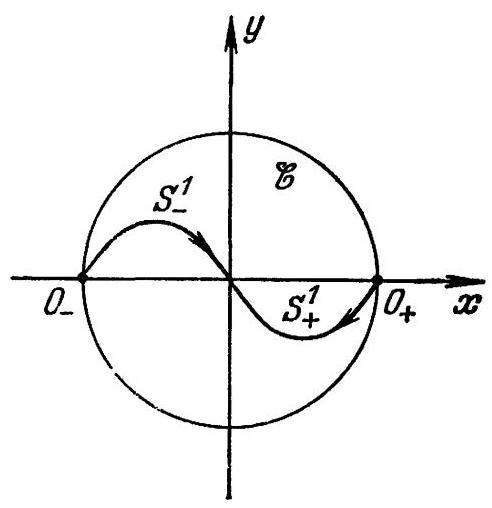
\includegraphics[max width=0.4\textwidth]{images/bo_d547k8bef24c73bgfcg0_55_927_780_492_508_0.jpg}
\end{center}
\hspace*{3em} 

Рис. 1.10. Оптимальное по быст- родействию управление, приво- дящее систему в начало коорди- нат. График кривой переключе- ния для системы х- 20 йх + 8 х = и. \(\left| {u\left( t\right) }\right|  \leq  1\) . C л y q a й 1 . п р н- мер 2: \({b}^{2} - {k}^{2} > 0,b > 0,{k}^{2} > 0\) :

Пусть \({S}_{ + }^{1}\) -дуга решения \({\mathcal{S}}_{ + }\) ,веду- щая из точки \({O}_{ + }\) в начало координат. Тогда кривая переключений у = W (х) состоит из дуги \({S}_{ + }^{1}\) при \(x \geq  0\) и соответ- ствующей дуги \({S}_{ - }^{1}\) системы \({\mathcal{S}}_{ - }\) при \(x \leq  0\) . Область управляемости € представляет собой открытую область, ограниченную решением системы S, идущим из точ- ки \({O}_{ + }\) в точку \({O}_{ - }\) при \(y \leq  0\) и решением системы \$\_, идущим из точки 0\_ в точку \({O}_{ + }\) при y≥0 (puc. 1.10). Как обычно, синтезирующая функция определена в области 6 (см. рис. 1.10) и имеет вид

\[
\Psi \left( {x,y}\right)  = \left\{  \begin{array}{lllll}  - 1 & \text{ для } & y > W\left( x\right) & \text{ и на } & {S}_{ - }^{1}, \\   + 1 & \text{ для } & y < W\left( x\right) & \text{ и на } & {S}_{ + }^{1}. \end{array}\right.
\]

Пример 3. Управление под действием отталкивающей силы. Рассмотрим синтез оптимального управления в задаче приведения к началу координат за минимальное время линейной системы

\[
\ddot{x} + {2b}\dot{x} - {k}^{2}x = u
\]

с постоянными коэффициентами \(b\) и \({k}^{2} > 0\) и ограничением \(\left| {u\left( t\right) }\right|  \leq  1\) . Здесь снова оптимальное управление и «(t) на интер- вале 0 \(\leq  t \leq  {t}^{ * }\) , переводящее произвольную точку ( \({x}_{0},{y}_{0}\) ), принад- лежащую области управляемости, в точку (0, 0), является единст- венным максимальным управлением, переводящим \(\left( {{x}_{0},{y}_{0}}\right)\) в (0,0) и

\[
{u}^{ * }\left( t\right)  = \operatorname{sgn}{\eta }_{2}\left( t\right) .
\]

Сопряженное решение \({\eta }_{2}\left( t\right)  \text{ ≢ } 0\) удовлетворяет уравнению

\[
{\ddot{\eta }}_{2} - {2b}{\dot{\eta }}_{2} - {k}^{2}{\eta }_{2} = 0
\]

и имеет не более одного нуля; общее решение имеет вид

\[
{\eta }_{2}\left( t\right)  = \alpha {e}^{bt}\operatorname{sh}\left( {{vt} + \beta }\right) ,
\]

где а и д — постоянные, а у у у те ты таким образом, и*(н) имеет не более, чем одно переключение.

Линия переключения составляется из двух кривых \({\Gamma }_{ + }\) и \({\Gamma }_{ - }\) . Здесь г\_фе- шение системы \$, проходящее через точку (0, 0) и лежащее в четвертом квад- ранте фазовой плоскости. Аналогично, решение Г\_ системы f\_ проходит через точку (0, 0) и находится во втором ква- дранте (рис. 1.11). Область управляе- мости представляет собой открытую бес-

\begin{center}
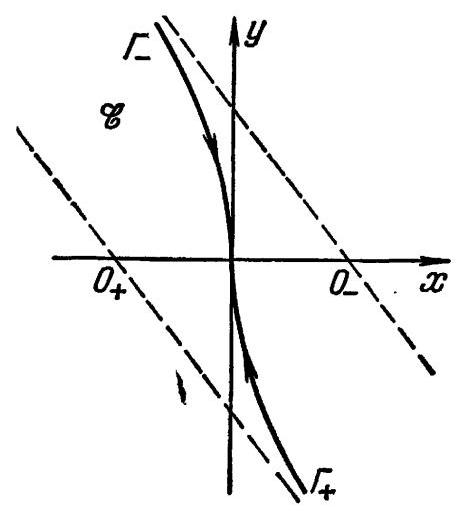
\includegraphics[max width=0.4\textwidth]{images/bo_d547k8bef24c73bgfcg0_56_160_687_459_511_0.jpg}
\end{center}
\hspace*{3em} 

Рис. 1.11. Оптимальное по быст- родействию управление, приво- дящее систему в начало коорди- нат. График кривой переключе- ния для системы х + 2bx – \({k}^{2}x = u\) , \(\left| {u\left( t\right) }\right|  \leq  1\) .

Экстремальные системы

\[
\left( {\mathcal{Y}}_{ - }\right) \;\dot{x} = y,\;\dot{y} = {k}^{2}x - {2by} - 1
\]

и

\[
\left( {\mathcal{S}}_{ + }\right) \;\dot{x} = y,\;\dot{y} = {k}^{2}x - {2by} + 1
\]

соответственно имеют особые точки 0\_: \(x = 1/{k}^{2},y = 0\) и \({O}_{ + } : x =  - 1/{k}^{2},y = 0\) , являющиеся особыми точками типа седла. конечную полосу, ограниченную прямыми

\[
y = \left( {-b - v}\right) \left( {x - \frac{1}{{k}^{2}}}\right)
\]

\(\mathrm{H}\)

\[
y = \left( {-b - v}\right) \left( {x + \frac{1}{{k}^{2}}}\right) .
\]

Картина не меняется при \(b > 0,b = 0\) и \(b < 0\) . Синтезирующая функция определяется как обычно:

\[
\Psi \left( {x,y}\right)  = \left\{  \begin{array}{llllll}  - 1 & \pi \mathrm{{PH}} & y > W\left( x\right) & \mathrm{H} & \mathrm{{На}} & {\Gamma }_{ - }, \\   + 1 & \pi \mathrm{{PH}} & y < W\left( x\right) & \mathrm{H} & \mathrm{{На}} & {\Gamma }_{ + }. \end{array}\right.
\]

Упражнения

1. Рассмотрите управление гамильтоновой системой:

\[
{\dot{x}}^{i} = \frac{\partial H}{\partial {y}^{i}} + {u}^{i},\;\dot{{y}^{i}} =  - \frac{\partial H}{\partial {x}^{i}} + {v}^{i},\;i = 1,2,\ldots ,n.
\]

Здесь \(\left( {{x}^{1},{x}^{2},\ldots ,{x}^{n},{y}^{1},\ldots ,{y}^{n}}\right)  = \left( {x,y}\right)\) ТО4Ka фазового пространства Р2", а функция Гамильтона H (к, у) принадлежит классу C2 в R2n. Управляющий вектор (и, v) удовлетворяет ограничению

\[
\left| {u}^{i}\right|  \leq  1,\;\left| {v}^{i}\right|  \leq  1.
\]

Пусть \(H\left( {x,y}\right)  > 0\) и |grad \(H\left( {x,y}\right)  \mid   > 0\) в \({R}^{2n} \smallsetminus  \left( {0,0}\right) ;H\left( {0,0}\right)  = 0\) и lim \(H\left( {x,y}\right)  =  + \infty\) . Покажите, что можно из любого начального со- \(\left| x\right|  + \left| y\right|  \rightarrow  \infty\) стояния \(\left( {{x}_{0},{y}_{0}}\right)\) перевести систему в заданную окрестность начала координат.

2. Рассмотрите нелинейное дифференциальное уравнение

\[
\ddot{x} + f\left( {x,\dot{x}}\right) \dot{x} + g\left( x\right)  = 0,
\]

где \(f\left( {x,y}\right)\) и \(g\left( x\right)  - \phi\) ункции из \({C}^{1}\) на фазовой плоскости \({R}^{2}\) . Положим \(f\left( {x,y}\right)  \geq  0\) и \({xg}\left( x\right)  > 0\) для \(x \neq  0\) .

(a) Покажите,что если функция \(G\left( x\right)  = {\int }_{0}^{x}g\left( s\right) {ds}\) удовлетворяет условию: \(\mathop{\lim }\limits_{{x \rightarrow  \infty }}G\left( x\right)  = \infty\) ,то каждая кривая

\[
V\left( {x,y}\right)  = \frac{{y}^{2}}{2} + G\left( x\right)  = {V}_{0} > 0
\]

представляет собой замкнутую кривую, содержащую внутри себя начало координат.

(b) Пусть \(f\left( {x,y}\right)  \equiv  0\) и \(g\left( x\right)  = x{e}^{-{x}^{2}}\) так,что нелинейное уравнение

\[
\ddot{x} + x{e}^{-{x}^{2}} = 0
\]

допускает линейную аппроксимацио

\[
\ddot{x} + x = 0
\]

вблизи начала координат. Покажите, что глобальное поведение решений этих уравнений на фазовой плоскости будет качественно различным.

3. Рассмотрите описанные ниже системы управления с указанными кри- териями качества и целевыми множествами. Покажите, что в каждом случае систему можно из любого начального состояния перевести в соответствующее целевое множество, однако оптимального управления не существует. Устано- вите в каждом случае, почему не применима теорема существования, уста- новленная в разделе 1.2.

(a) \(\dot{x} = \sin {2\pi u},\;\dot{y} = \cos {2\pi u},\;\dot{z} =  - 1\) в \({R}^{3}\) при условии \(\left| {u\left( t\right) }\right|  \leq  1\) .

Начальное состояние (0, 0, 1), конечное—(0, 0, 0); критерий качества —

\[
C\left( u\right)  = {\int }_{0}^{t}\left( {{x}^{2} + {y}^{2}}\right) {dt}
\]

Указание. Постройте управления \({u}_{k}\left( t\right)\) на \(0 \leq  t \leq  1\) , удовлетворяю- щие соотношениям

\(\sin {2\pi }{u}_{k}\left( t\right)  = \sin {2\pi kt};\;\cos {2\pi }{u}_{k}\left( t\right)  = \cos {2\pi kt}\) для \(k = 1,2,3\ldots\) ;

(b) \(x = u,y = v,z =  - 1\) B \({R}^{3}\) при условии \({u}^{2}\left( t\right)  + {v}^{2}\left( t\right)  = 1\) . Переведите \(\left( {0,0,1}\right)\) в \(\left( {0,0,0}\right)\) . Критерий качества

\[
C\left( {u,v}\right)  = {\int }_{0}^{t}\left( {{x}^{2} + {y}^{2}}\right) {dt}
\]

(c) \(x = 1,y =  - x{e}^{y}u\) B \({R}^{2}\) при условии \(0 \leq  u\left( t\right)  \leq  2\) . Переведите (—1,0) в (1,0). Критерий качества

\[
C\left( u\right)  = {\int }_{0}^{t}\left( {2 - y}\right) {dt} = {\int }_{-1}^{1}\left( {2 - y}\right) {dx}.
\]

Указание. Для каждого решения \(x\left( t\right)  = t - 1,y\left( t\right)\) покажите, что \(0 \leq  y\left( x\right)  \leq   - \ln {x}^{2}\) для \(x \neq  0\) . Тогда \(C\left( u\right)  > {\int }_{-1}^{1}\left( {2 + \ln {x}^{2}}\right) {dx} = 0\) . Попробуйте применить управление \({u}_{\varepsilon }\left( t\right)  = 2 - \varepsilon\) для малых \(\varepsilon  > 0\) .

4. Рассмотрите нелинейную систему

\[
\ddot{x} - {\dot{x}}^{2} - {x}^{2} = {u}^{2},\;\left| {u\left( t\right) }\right|  \leq  1
\]

в фазовой плоскости \(x,y = x\) . Покажите, что область нуль-управляемости це- ликом лежит в четвертом квадранте и, следовательно, не содержит никакой окрестности начала координат.

5. Запишите линейную систему с постоянными коэффициентами

\[
{x}^{\left( n\right) } + {a}_{1}{x}^{\left( n - 1\right) } + \ldots  + {a}_{n}x = u
\]

в виде матричной системы первого порядка

(F)
\[
\dot{x} = {Ax} + {bu},
\]

положив x1=x, x²=x’, …, x’=x’=(n-1). Используя теоремы, доказанные в разделе 1.3, покажите, что система \$ управляема.

6. Рассмотрите нелинейный управляемый процесс

\[
{x}^{\left( n\right) } + f\left( {x,\dot{x},\ddot{x},\ldots ,{x}^{\left( n - 1\right) },u}\right)  = 0,
\]

где функция \(f\left( {{x}^{1},\ldots ,{x}^{n},u}\right)\) принадлежит С 1 в Rn+1, а управление и под- чинено ограничению \(\left| {u\left( t\right) }\right|  \leq  1\) . Кроме того, \(f\left( {0,0,\ldots ,0}\right)  = 0\) и \(\frac{\partial f}{\partial u}\left( {0,\ldots ,0}\right)  \neq  0.\) Применяя теоремы, сформулированные в разделе 1.3, покажите, что область нуль-управляемости для соответствующей системы уравнений первого порядка в \({R}^{n}\) содержит открытую окрестность начала координат.

7. Покажите, что система

(F)
\[
\dot{x} =  - x + u,\;\dot{y} =  - {2y}
\]

не является управляемой в R2, исследуя картину интегральных кривых на фазовой плоскости. Произведя преобразование координат,

\[
\bar{x} = {2x} - y,\;\bar{y} = x - y,
\]

получите соответствующую систему у. Проверьте, выполняется ли для нее алгебраическое условие управляемости раздела 1.3.

8. Рассмотрите примеры 1 и 2 раздела 1.2.

(a) Покажите, что система может быть приведена в начало координат из любого начального состояния.

(b) Проверьте в каждом случае выполнение всех условий теоремы сущест- вования раздела 1.2 и докажите существование управления, оптимального по быстродействию.

9. (a) Рассмотрите нелинейную автономную систему

(F)
\[
\dot{x} = f\left( {x,u}\right) \text{ при }u\left( t\right)  \in  \Omega ,
\]

переводящую \({x}_{0}\) в \({x}_{1} = 0\) и минимизирующую \(C\left( u\right)  = {\int }_{0}^{t}{f}^{0}\left( {x\left( t\right) ,u\left( t\right) }\right) {dt}\;\mathrm{K}\)

в разделе 1.4. Сформулируйте в терминах управления \(u\left( t\right)\) и решений \(x\left( t\right)\) , \(\eta \left( t\right)\) принцип максимума для оптимального управления.

(b) Сформулируйте соответствующий принцип для управления, максими- зирующего критерий \(C\left( u\right)\) .

10. Рассмотрите систему

\[
\dot{x} = u - {u}^{2}
\]

с ограничением |u (t)|≤1. Покажите, что оптимальным управлением, пере- водящим \({x}_{0} =  - 1\) в \({x}_{1} = 0\) за минимальное время,будет и (t) \(\equiv  \frac{1}{2}\) . Отметим. что в данном случае оптимальное управление не будет релейной функцией, переключающейся с +1 на -1.

Приложение I

\section*{Геометрическая теория обыкновенных дифференциальных уравнений}

В примерах 2 и 3 раздела 1.1 мы показали, как свести изу- чение одного уравнения второго порядка, напрнмер,

\[
\ddot{x} = f\left( {t,x,\dot{x}}\right) ,
\]

к изучению системы двух дифференциальных уравнений первого порядка:

\[
x = y,\;\dot{y} = f\left( {t,x,y}\right) .
\]

Аналогичным образом, вместо скалярного дифференциального уравнения высшего порядка можно рассматривать соответствую- щее векторное уравнение первого порядка, представляющее собой частный случай системы дифференциальных уравнений первого порядка:

\[
{\dot{x}}^{1} = {f}^{1}\left( {t,{x}^{1},\ldots ,{x}^{n}}\right) ,
\]

\[
{\dot{x}}^{2} = {f}^{2}\left( {t,{x}^{1},\ldots ,{x}^{n}}\right) ,
\]

\[
{\dot{x}}^{n} = {f}^{n}\left( {t,{x}^{1},\ldots ,{x}^{n}}\right) .
\]

Эту систему дифференциальных уравнений можно записать так;

\[
\dot{{x}^{i}} = {f}^{i}\left( {t,{x}^{1},\ldots ,{x}^{n}}\right)  = {f}^{i}\left( {t,x}\right) ,\;i = 1,2,\ldots ,n,
\]

или в виде векторного дифференциального уравнения

(F)
\[
x = f\left( {t,x}\right) \;\text{ или }\;\frac{dx}{dt} = f\left( {t,x}\right)
\]

Решение

\[
x\left( t\right)  = \left[ \begin{array}{c} {x}^{1}\left( t\right) \\  \cdots \\  {x}^{n}\left( t\right) \end{array} \right]
\]

представляет собой вектор-столбец, состоящий из действительных дифференцируемых функций аргумента t, определенных на неко- тором открытом интервале 9 и удовлетворяющих на нем системе дифференциальных уравнений \({x}^{i}\left( t\right)  = {f}^{i}\left( {t,x\left( t\right) }\right) ,i = 1,2,\ldots ,n\) .

В этом разделе предлагается геометрическая интерпретация векторного дифференциального уравнения \$ как векторного по- ля в пространстве R" п действительных переменных ( \({x}^{1}\) , …, \({x}^{n}\) ). Кроме того, мы введем терминологию и обозначения, употребляе- мые в теории векторных и скалярных функций и сформулируем основные теоремы, относящиеся к векторным дифференциальным уравнениям. При желании читатель может лишь бегло ознако- миться с этим материалом, возвращаясь к нему для детального изучения по мере того, как отмеченные здесь понятия будут встречаться в излагаемой далее теории оптимального управления.

Обозначение множеств в R", n=1, 2, 3, ...

Пространство \({R}^{n}\) представляет собой совокупность всевозмож- ных наборов n действительных чисел \(\left( {{x}^{1},\ldots ,{x}^{n}}\right)\) . Таким образом, \({R}^{1}\) есть действительная прямая, а \({R}^{2}\) —действительная плоскость. Если точка или вектор \({x}_{0} = \left( {{x}_{0}^{1},\ldots ,{x}_{0}^{n}}\right)\) принадлежит некоторому подмножеству \(A\) из \({R}^{n}\) , то пишут \({x}_{0} \in  A\) . Если каждая точка A лежит в подмножестве B, т. е. А содержится в В, то пишут Ас В. Множество точек, принадлежащих ди, но не принадлежащих да, называют разностью множеств \({A}_{1}\) и \({A}_{2}\) и обозначают \({A}_{1} - {A}_{2}\) ; если же \({A}_{1} \subset  {A}_{2}\) , to разность их будет пустым множеством,т. е. мно- жеством, не содержащим ни одной точки. Пересечением А, 1, A, называется множество точек в \({R}^{n}\) ,принадлежащих как \({A}_{1}\) ,так и \({A}_{2}\) , а объединением А1 U А2 — множество точек, принадлежащих хотя бы одному из множеств А1 или А2; аналогично определяются пере- сечение и объединение любого конечного числа подмножеств в R".

Для множеств Асе \({R}^{n}\) и ВС, \({R}^{m}\) мы определяем их произведение \(A \times  B \subset  {R}^{n + m}\) как множество всех пар точек \(\left( {x,y}\right)\) ,где \(x \in  A,y \in  B\) .

Понятия \({P}_{0} \in  S,A \subset  B,{A}_{1} - {A}_{2},{A}_{1} \cap  {A}_{2},{A}_{1} \cup  {A}_{2}\) и \(A \times  B\) для подмножеств более общих пространств определяются аналогично.

\section*{Геометрия в R"}

Нам понадобится в дальнейшем следующая норма в \({R}^{n}\) (не совпадающая с евклидовой):

\[
\left| {x}_{0}\right|  = \left| {x}_{0}^{1}\right|  + \left| {x}_{0}^{2}\right|  + \ldots  + \left| {x}_{0}^{n}\right| ,\;{x}_{0} = \left( {{x}_{0}^{1},{x}_{0}^{2},\ldots ,{x}_{0}^{n}}\right)  \in  {R}^{n}.
\]

С введением расстояния между точкамн \(x\) и \(y\) по формуле \(d\left( {x,y}\right)  = \left| {x - y}\right| ,{R}^{n}\) превращается в метрическое пространство, т. е. пространство, в котором определена действительная функция расстояния, удовлетворяющая следующим аксиомам:

1. \(d\left( {{x}_{0},{y}_{0}}\right)  > 0\) , если \({y}_{0} \neq  {x}_{0}\) и \(d\left( {{x}_{0},{x}_{0}}\right)  = 0\) .

2. \(d\left( {{x}_{0},{y}_{0}}\right)  = d\left( {{y}_{0},{x}_{0}}\right)\) .

3. \(d\left( {{x}_{0},{z}_{0}}\right)  \leq  d\left( {{x}_{0},{y}_{0}}\right)  + d\left( {{y}_{0},{z}_{0}}\right)\) .

Множество б С Гви пазывается открытым, если для каждой точки \({x}_{0} \in  6\) cyществует число r > 0 такое,что множество точек \(\left\{  {x\left| {x \in  {R}^{n}}\right|  : \left| {x - {x}_{0}}\right|  < r}\right\}\) целиком лежит в 6 (замена нормы | \(x - {x}_{0}\) | евклидовой длиной х—х, привела бы к точно такому же опреде- лению). Множество \(C \subset  {R}^{n}\) называется замкнутым, если множество \({R}^{n} - C\) открыто в \({R}^{n}\) . Открытое множество \(\varnothing  \subset  {R}^{n}\) не содержит своих граничных точек, в то время как замкнутое множество \(C \subset  {R}^{n}\) содержит все свои граничные точки. Объединение открытых множеств есть открытс - множество, а пересечение замкнутых — зам- кнутое множество. Объединение всех открытых множеств, содер- жащихся в некотором множестве Ас- R", называется внутренностью множества A. Множество N с R", содержащее множество A в своей внутренности, называется окрестностью множества А. Пересече- ние \(\bar{A}\) всех замкнутых множеств в \({R}^{n}\) ,каждое из которых содер- жит \(A\) ,называется замыканием множества А в R". Говорят, что точка \(P\) принадлежит границе д \(A\) множества А, если каждая окрестность \(P\) содepжит как точки, принадлежащие A, так и точки, принадлежащие его дополнению \({R}^{n} - A\) . Все эти определения и свойства открытых и замкнутых множеств верны в любом мет- рическом пространстве.

Множество \(K \subset  {R}^{n}\) называется компактным, если \(K\) замкнуто и ограничено в \({R}^{n}\) (т. e. \(K\) замкнуто и функция |x| orраничена на K). Расстоянием от точки РЕ Р" до компактного множества \(K \subset  {R}^{n}\) называется кратчайшее евклидово расстояние от \(P\) до точек множества \(K\) . Множество \(A \subset  {R}^{n}\) называется выпуклым, если для любой пары точек \({x}_{0}\) и \({x}_{1}\) из \(A\) весь отрезок \(\mu {x}_{0} + \left( {1 - \mu }\right) {x}_{1}\) ,где \(0 \leq  \mu  \leq  1\) ,лежит в А (здесь линейная комбинация векторов вы- числяется покомпонентно). Открытое множество 6 с связным, если любые две точки из 6 можно соединить непрерыв- ной кривой, лежащей в 6. Заметим, что всё пространство R" яв- ляется открытым, замкнутым, выпуклым и связным в R", но не является компактным.

Система *дифференциальных уравнений

\[
f\left( \mathcal{G}\right) \;{x}^{i} = {f}^{i}\left( {t,{x}^{1},\ldots ,{x}^{n}}\right) ,\;i = 1,2,\ldots ,n
\]

может быть интерпретирована геометрически, как векторное поле с компонентами \({\dot{f}}^{i}\left( {\dot{t},x}\right)\) в каждый момент времени t в пространстве \({R}^{n}\) . Мы называем \({R}^{n}\) ,или его подмножество,в котором опреде- лена система 8, фазовым пространством системы 5. Решение системы \$ в R" представляет собой кривую х (t) = (x'(t)), задан- ную в параметрическом виде (с параметром t), касательный вектор которой или вектор скорости х (t) = ( \({\dot{x}}^{i}\left( t\right)\) ) совпадает с вектором \(f\left( {t,x\left( t\right) }\right)\) .

Если вектор-функция \(f\left( {t,x}\right)\) не зависит от времени, т. е. \(f\left( {t,x}\right)  \equiv  f\left( x\right)\) , то система дифференциальных уравнений называется автономной. В этом случае векторное поле 8 можно представить как поле скорости установившегося потока жидкости в R". Если \(f\left( {x}_{0}\right)  = 0\) ,то \({x}_{0}\) есть особая точка, или точка равновесия автоном- ной системы \$, а х (t) = х。— решение, которое на фазовой плоскос- ти изображается одной точкой. Периодическое решение \(x\left( t\right)\) cu- стемы, т. е. такое, что для некоторого постоянного периода P > 0 имеет место тождество \(x\left( t\right)  = x\left( {t + P}\right)\) , изображается в фазовом пространстве в виде простой замкнутой кривой. Этот геометри- ческий язык полезен при исследовании качественной картины поведения интегральных кривых системы S.

Для того чтобы сформулировать фундаментальные теоремы существования, единственности и регулярности решений \$, необ- ходимо ввести понятия непрерывности и дифференцируемости.

\section*{Определения непрерывности и дифференцируемости в R"}

Векторная функция \(f\left( x\right)\) co значениями в \({R}^{n}\) называется непре- рывной на множестве Асе л’, если каждая ее компонента f’ ( \({x}^{1},\ldots ,{x}^{n}\) ) является непрерывной функцией на \(A\) . Далее, говорят, что f(x) принадлежит классу \({C}^{k}\) , где k=1, 2, 3, ..., на открытом мно- жестве \(\mathcal{C} \subset  {R}^{n}\) , если каждая ее компонента \({f}^{i}\left( {{x}^{1},\ldots ,{x}^{n}}\right)\) непре- рывна и имеет непрерывные частные производные порядка \(\leq  k\) на множестве 6. Если f(x) принадлежит всем классам \({C}^{k}\) ,то пишут \(f\left( x\right)  \in  {C}^{\infty }\) на \(\mathcal{C}\) . Echu \(f\left( x\right)\) является аналитической функцией на 6, т. е. если каждая функция \({f}^{i}\left( {{x}_{1},\ldots ,{x}^{n}}\right)\) разлагается в абсолютно сходящийся степенной ряд в окрестности каждой точки хеб, то отсюда следует, что \(f\left( x\right)  \in  {C}^{\infty }\) . Как было отмечено ранее, произ- водной векторной функции \(x\left( t\right)  = \left( {{x}^{i}\left( t\right) }\right)\) no \(t \in  {R}^{1}\) называется вектор- функция \(\dot{x}\left( t\right)  = \left( {{\dot{x}}^{i}\left( t\right) }\right)\) .

Рассмотрим действительную систему дифференциальных урав- нений\(\left( \mathcal{S}\right)\)

\[
{\dot{x}}^{i} = {f}^{i}\left( {t,{x}^{1},\ldots ,{x}^{n}}\right) ,\;i = 1,2,\ldots ,n,
\]

где функция \(f\left( {t,x}\right)\) определена и непрерывна на \(\mathcal{I} \times  \mathcal{O} \subset  {R}^{1 + n}\) , \(J \subset  {R}^{1}\) -открытый интервал, а 6 -открытое множество в R". Предположим, что функции \(\partial {f}^{i}\left( {t,x}\right) /\partial {x}^{j}\) непрерывны на \(J \times  6\) . Тогда для каждой начальной точки \(\left( {{t}_{0},{x}_{0}}\right)  \in  J \times  6\) cyществует единственное решение системы S:

\[
x = \varphi \left( {t,{t}_{0},{x}_{0}}\right) ,
\]

проходящее через заданную точку \({x}_{0}\) в момент времени б,

\[
\varphi \left( {{t}_{0},{t}_{0},{x}_{0}}\right)  = {x}_{0}
\]

и это решение определено в 9х60 на некотором максимальном промежутке времени т. ( t, 0, x, c) < t < τ+ (t, x, 0), где оно удовлетво- ряет системе Я. Эта основная теорема существования и единст- венности доказывается в учебниках по теории обыкновенных дифференциальных уравнений.

Однако нам понадобится более сильная теорема существования, нежели описанная выше, так как нам придется иметь дело с си- стемами дифференциальных уравнений, у которых коэффициенты \(f\left( {t,x}\right)\) являются разрывными функциями от \(t\) . Такие системы играют важную роль в теории оптимального управления, поскольку они описывают поведение управляемого объекта под действием оптимальных управлений с мгновенными переключениями. Мы будем всегда считать, что f’ и x) — измеримые по t функции для любого фиксированного х. Измеримые функции действительного переменного \(t\) cocтавляют весьма обширный класс функций, вклю- чающий в себя все непрерывные функции, кусочно-непрерывные функции, а также пределы таких функций. Довольно затрудни- тельно привести пример неизмеримой функции; во всяком случае, мы будем сталкиваться лишь с измеримыми функциями (чаще всего с кусочно-непрерывными). Ниже мы дадим краткие сведения о функциях, измеримых и интегрируемых по Лебегу.

\section*{Определения измеримых и интегрируемых функций на R" Слабая компактность}

Подмножество N с R" называется множеством меры нуль, если для него найдется покрытие, представляющее собой объединение счетного числа n-мерных кубов, общий объем которых меньше заранее заданного числа вс>0. Например, любое конечное или бесконечное счетное множество точек в R \textdegree  является множеством меры нуль. О двух функциях \({f}_{1}\left( x\right)\) и \({f}_{2}\left( x\right)\) , onределенных на \(A \subset  {R}^{n}\) и отличающихся друг от друга на множестве меры нуль, говорят, что они совпадают почти всюду на \(A\) . Измеримые 1) множества в \({R}^{n}\) определяются, как элементы некоторого наименьшего се- мейства множеств в \({R}^{n}\) , содepжащего все открытые множества, все замкнутые множества, все множества меры нуль из R", раз- ность любых двух членов этого семейства, а также объединения и пересечения конечного или счетного числа любых его элементов. Действительная функция \(h\left( t\right)\) , ompeделенная на действительном интервале J, называется измеримой, если для любых действи- тельных а и р множество \{t∣t∈J u α<h(t)<β\} является из- меримым в \({R}^{1}\) . Если функция \(h\left( t\right)\) измерима на \(\mathcal{I}\) , to существует замкнутое подмножество € в 9 такое, что функция \(h\left( t\right)\) непрерыв- на на \(\mathcal{C}\) , a мера множества 9-е сколь угодно мала 1).

\HRule

1) Речь идет об измеримости в смысле Лебега. (Прим. ред.)

\HRule

Если функция \(h\left( t\right)\) измерима на \(\mathcal{J}\) ,то мы можем определить для нее интеграл Лебега

\[
{\int }_{\mathcal{Y}}{h}_{a}\left( t\right) {dt}
\]

рассматривая соответствующие пределы интегральных сумм. Функ- ция \(h\left( t\right)\) называется интегрируемой на 9, если записанный выше интеграл, а также интеграл от |h(t)| суть конечные действитель- ные числа. Изменение значений функции \(h\left( t\right)\) на множестве меры нуль не влияет на величину интеграла. Если функция \(h\left( t\right)\) ку- сочно-непрерывна, а интервал 7 компактен, то значение написан- ного выше интеграла Лебега совпадает со значением обычного риманова интеграла.

Пусть \(h\left( t\right)\) интегрируема на интервале \(\mathcal{I} = \left( {{t}_{0},{t}_{1}}\right)\) . Рассмотрим неопределенный интеграл

丨

\[
H\left( t\right)  = {\int }_{{t}_{0}}^{t}h\left( s\right) {ds}\text{ для }{t}_{0} \leq  t \leq  {t}_{1}.
\]

Такой интеграл представляет собой абсолютно непрерывную функ- цию 2). Можно доказать, что абсолютно непрерывная функция непрерывна и дифференцируема почти всюду (т. е. на всем интер- вале 9, исключая множество меры нуль), и имеет место равенство (также почти всюду):

\[
\frac{d}{dt}H\left( t\right)  = h\left( t\right)
\]

Всякая липшицева непрерывная функция \(H\left( \widetilde{t}\right)\) является абсолют- но непрерывной 3). Таким образом, основное отличие, возникающее из-за разрывности \(f\left( {t,x}\right)\) , состоит в том,что многие из обычных формул дифференциального и интегрального исчисления верны лишь «почти всюду».

\HRule

1) Это есть следствие известной теоремы Н. Н. Лузина о С-свойстве измеримой функции, которое может быть положено в основу самого определе- ния измеримости. (Прим. ред.),

29 Функция f, заданная на интервале У, называется абсолютно непрерыв- ной на J, если для любого в > 0 найдется δ>0 такое, что для любой конечной системы попарно непересекающихся интервалов \({y}_{k} = \left( {{a}_{k},{b}_{k}}\right) (k = 1\) , 2, . . ., n) из J с общей длиной, не превосходлией δ, выполнено неравенство

\[
\mathop{\sum }\limits_{{k = 1}}^{n}\left| {f\left( {b}_{k}\right)  - f\left( {a}_{k}\right) }\right|  < \varepsilon
\]

(Прим. ред.)

3) Говорят, что функция \(f\left( x\right)\) на интервале (а, b) удовлетворяет условию Липшица порядка α (0 < α ≤ 1), если существует константа А такая, что для всех х, и, из из (a, b) имеет место неравенство \(\left| {f\left( {x}_{2}\right)  - f\left( {x}_{1}\right) }\right|  \leq  A{\left| {x}_{2} - {x}_{1}\right| }^{\alpha }\) . (Прим. ред.)

\HRule

В дальнейшем при доказательстве существования оптимальных управлений нам потребуется понятие слабой сходимости последо- вательности управлений. Последовательность \(\{ {u}_{n}\left( t\right) \} ,n = 1,2,3,\ldots\) действительных или векторных интегрируемых функций на неко- тором действительном интервале 9 называется слабо сходящейся к функции \({u}^{ * }\left( t\right)\) , если для любой ограниченной измеримой весовой функции \(g\left( t\right)\) имеем

\[
\mathop{\lim }\limits_{{n \rightarrow  \infty }}{\int }_{y}g\left( t\right) {u}_{n}\left( t\right) {dt} = {\int }_{y}g\left( t\right) u * \left( t\right) {dt}
\]

Можно показать, что множество всех измеримых на конечном интервале J и принимающих значения из некоторого компактного выпуклого подмножества Ω⊂R™ векторных функций является слабо компактным. Это означает, что из каждой последователь- ности таких функций можно выделить подпоследовательность, слабо сходящуюся на 9 к функции из данного множества. Разумеется, предельная функция и*(t) определена лишь почти всюду на 9.

Множество всех действительных функций, определенных на интервале 9, для которых

\[
{\int }_{y}{\left| u\left( t\right) \right| }^{p}{dt} < \infty \;\left( {1 \leq  p < \infty }\right)
\]

составляет пространство \({L}_{p}\) . Если отождествить функции, отли- чающиеся друг от друга лйшь на множестве меры нуль, и ввести норму по формуле

\[
\parallel u{\parallel }_{p} = {\left( {\int }_{\mathcal{J}}{\left| u\left( t\right) \right| }^{p}dt\right) }^{\frac{1}{p}}
\]

то \({L}_{p}\) станет полным нормированным векторным пространством (такие пространства часто называют банаховыми). Под пространст- вом \({L}_{\infty }\) мы понимаем множество всех существенно ограниченных, или ограниченных почти всюду измеримых функций с нормой \(\{ u{\parallel }_{\infty } =\) ess \(\sup {\left| u\left( t\right) \right| }^{1}\) ). Если 9-компакт, то выполняется соот- ношение \({L}_{p} \subset  {L}_{1}\) для \(1 \leq  p \leq  \infty\) .

Замкнутый шар в \({L}_{p}\) для \(1 < p \leq  \infty\) (т. е. множество ∥ \(u{ \parallel  }_{p} \leq  B\) ) является слабо компактным; на самом деле, соответствующая последовательность интегралов сходится для любой весовой функции \(g\left( t\right)  \in  {L}_{q}\) на \(g\) , если \(\frac{1}{p} + \frac{1}{q} = 1\) . В частности, если \(p = 1\) , то \(q = \infty\) . Случай \(p = q = 2\) представляет особый интерес, и \({L}_{2}\) на- зывают гильбертовым пространством.

\HRule

1) По определению, ess sup \(\left| {u\left( t\right) }\right|  = \mathop{\inf }\limits_{{v\left( t\right) }}\mathop{\sup }\limits_{{t \in  \mathcal{J}}}\left| {v\left( t\right) }\right|\) ,где \(v\left( t\right)\) пробегает мно- жество всех ограниченных измеримых функций на \(\mathcal{I}\) , совпадающих с и (t) почти всюду. (Прим. ред.)

\HRule

По определению, вектор (или матрица) и (и) принадлежит L, на интервале 9, 1 ≤ p ≤ ∞, если каждая из его компонент и i < принадлежит \({L}_{p}\) . Это будет тогда и только тогда, когда

\[
{\int }_{y}{\left| u\left( t\right) \right| }^{p}{dt} < \infty
\]

Приступим теперь к формулировке основной теоремы существова- ния, единственности и регулярности для систем дифференциальных уравнений. Доказательство и подробное обсуждение ее можно найти в соответствующих учебниках.

Teopeма IA. Рассмотрим систему дифференциальных урав- нений

(5)
\[
{\dot{x}}^{i} = {f}^{i}\left( {t,{x}^{1},\ldots ,{x}^{n}}\right) ,\;i = 1,\ldots ,n,
\]

где f(t, x) определено на некотором открытом множестве \(J \times  6 \subset  {R}^{n + 1}\) . Предположим, что

(a) \(\partial \Lambda \Re\) любого фиксированного \(t \in  \mathcal{I}\;{\phi y}\) нкции \({f}^{i}\left( {t,x}\right)\) принад- лежат классу \({C}^{1}\) для \(x \in  \mathcal{O}\) ;

(b) для любого фиксированного \(x \in  \mathcal{O}\) функции \({f}^{i}\left( {t,x}\right)\) измерим. no \(t\) на \(\mathcal{I}\) ;

(c) для любой пары компактных подмножеств J \textdegree С 9 и K=O существует интегрируемая функция \(m\left( t\right)\) на \({g}_{c}\) , maкая,что

\[
\left| {f\left( {t,x}\right) }\right|  \leq  m\left( t\right) \text{ и }\left| {\frac{\partial f}{\partial x}\left( {t,x}\right) }\right|  \leq  m\left( t\right)
\]

\(\partial \pi\) я всех (t, \(x) \in  {\mathcal{I}}_{c} \times  K\) .

Тогда для любых начальных условий (t, 0, 0) из J × 6 существует единственное решение системы S

\[
x = \varphi \left( {t,{t}_{0},{x}_{0}}\right) ,
\]

maкое, чмо

\[
\varphi \left( {{t}_{0},{t}_{0},{x}_{0}}\right)  = {x}_{0},
\]

опребгенное иа иекопором максцмальтом променсуmке временц

\[
{\tau }_{ - }\left( {{t}_{0},{x}_{0}}\right)  < t < {\tau }_{ + }\left( {{t}_{0},{x}_{0}}\right) .
\]

Кроме того, вектор-функция q (t, t, o, u) определена и непрерывна на некотором открытом множестве D C R1+1-n. Для любых фик- сированных \({t}_{0}u{x}_{0}\) функция \(\varphi \left( {t,{t}_{0},{x}_{0}}\right)\) абсолютно непрерывна no t и удовлетворяет векторному дифференциальному уравнению

\[
\frac{{d\varphi }\left( {t,{t}_{0},{x}_{0}}\right) }{dt} = f\left( {t,\varphi \left( {t,{t}_{0},{x}_{0}}\right) }\right)
\]

почти всюду на \({\tau }_{ - } < t < {\tau }_{ + }\) . Для любых фиксированных t и t, функция \(\varphi \left( {t,{t}_{0},{x}_{0}}\right)\) npинадлежит классу \({C}^{1}\) no \({x}_{0}\) и вектор-функция

\[
\frac{\partial \varphi \left( {t,{t}_{0},{x}_{0}}\right) }{\partial {x}_{0}^{j}},\;j = 1,2,\ldots ,n
\]

абсолютно непрерывна по t и удовлетворяет линейной системе дифференциальных уравнений

\[
\frac{d}{dt}\left( \frac{\partial {\varphi }^{i}}{\partial {x}_{0}^{j}}\right)  = \mathop{\sum }\limits_{{k = 1}}^{n}\frac{\partial {f}^{i}}{\partial {x}^{k}}\left( {t,\varphi \left( {t,{t}_{0},{x}_{0}}\right) }\right) \left( \frac{\partial {\varphi }^{k}}{\partial {x}_{0}^{j}}\right) .
\]

Эта основная теорема имеет большое число различных обоб- щений и модификаций. Мы перечислим их в следующих заме- чаниях.

3 амечания. 1. Предположим, что коэффициенты f(t, x, λ) системы \$ зависят от действительного векторного параметра \(\lambda  = \left( {{\lambda }^{1},\ldots ,{\lambda }^{m}}\right)\) . Если \(f\left( {t,x,\lambda }\right)\) onpeдeлeнa на открытом мно- жестве \(\mathcal{I} \times  \mathcal{O} \times  \Lambda  \subset  {R}^{1 + n + m}\) и если для каждого \({\lambda }_{0} \in  \Lambda\) выполня- ются предположения (а), (b) и (c) нашей теоремы, то система \$ имеет решение

\[
x = \varphi \left( {t,{t}_{0},{x}_{0},{\lambda }_{0}}\right) ,
\]

проходящее через точку ( \({t}_{0},{x}_{0}\) ) при \(\lambda  = {\lambda }_{0}\) . Далее, если предпо- ложения (а) и (с) усилить следующим образом:

(a’) для любого фиксированного \(t \in  \mathcal{I}\) функции \({f}^{i}\left( {t,x,\lambda }\right)\) при- надлежат классу \({C}^{k}\left( {k = 1,2,3,\ldots }\right)\) no \(\left( {x,\lambda }\right)\) из \(\varnothing  \times  \Lambda\) и

(c’) для любой тройки компактных подмножеств \({\mathcal{I}}_{c} \subset  \mathcal{I},K \subset  \mathcal{O}\) , \(L \subset  \Lambda\) cyществует интегрируемая функция \(m\left( t\right)\) на \({\mathcal{I}}_{c}\) ,такая,что

\[
\left| {{Df}\left( {t,x,\lambda }\right) }\right|  \leq  m\left( t\right) \text{ для всех }\left( {t,x,\lambda }\right)  \in  {\mathcal{I}}_{c} \times  K \times  L
\]

и для любого частного дифференцирования D порядка ≤k по \(\left( {x,\lambda }\right)\) , то решение \(\varphi \left( {t,{t}_{0},{x}_{0},\lambda }\right)\) будет непрерывной функцией на некотором открытом множестве 6′ с R1+1+n+m, принадлежащей классу \({C}^{k}\) no \(\left( {{x}_{0},\lambda }\right)\) .

2. Если функция \(f\left( {t,x,\lambda }\right)\) непрерывна на множестве \(9 \times  6 \times  \Lambda  \subset  {R}^{1 + n + m}\) и удовлетворяет предположениям (а’) и (с’), то предположение (b) выполняется автоматически. В этом случае решенне \(\varphi \left( {t,{t}_{0},{x}_{0},\lambda }\right)\) принадлежитклассу \({C}^{1}\) в \({\text{ б }}^{\prime } \subset  {R}^{1 + 1 + n + m}\) и удовлегворяет системе \({\mathcal{G}}^{ \circ  }\) вкаждой точкеннтервала \({\tau }_{ - } < t < {\tau }_{ + }\) .

3. Bo многих задачах можно установить, что макснмальный промежуток времени \({\tau }_{ - } < t < {\tau }_{ + }\) неграничен справа \(\left( {{\tau }_{ + } =  + \infty }\right)\) . B частности (как можно показать),такибудег,если \(J = \left( {{t}_{0}, + \infty }\right)\) и решение, проходящее через точку ( \({t}_{0}\) , \({x}_{0}\) ), лежит в компактном подмножестве K=6c=R" для \(t \geq  {t}_{0}\) .

Приложение II

\section*{Алгебраическая теория линейных дифференциальных уравнений}

В примерах 2 и 3 раздела 1 исследовались линейные процессы управления, описываемые дифференциальными уравнениями вто- рого порядка, причем задача сводилась к изучению систем диффе- ренциальных уравнений первого порядка на фазовой плоскости. Линейные процессы более высоких порядков сводятся к линейным системам, имеющим следующий общий вид:

\[
{\dot{x}}^{1} = {a}_{1}^{1}\left( t\right) {x}^{1} + {a}_{2}^{1}\left( t\right) {x}^{2} + \ldots  + {a}_{n}^{1}\left( t\right) {x}^{n} + {b}_{1}^{1}\left( t\right) {u}^{1} + \ldots  + {b}_{m}^{1}\left( t\right) {u}^{m},
\]

\[
{x}^{2} = {a}_{1}^{2}\left( t\right) {x}^{1} + {a}_{2}^{2}\left( t\right) {x}^{2} + \ldots  + {a}_{n}^{2}\left( t\right) {x}^{n} + {b}_{1}^{2}\left( t\right) {u}^{1} + \ldots  + {b}_{m}^{2}\left( t\right) {u}^{m},
\]

..........................

\[
\dot{{x}^{n}} = {a}_{1}^{n}\left( t\right) {x}^{1} + {a}_{2}^{n}\left( t\right) {x}^{2} + \ldots  + {a}_{n}^{n}\left( t\right) {x}^{n} + {b}_{1}^{n}\left( t\right) {u}^{1} + \ldots  + {b}_{m}^{n}\left( t\right) {u}^{m}.
\]

Эта линейная система дифференциальных уравнений описывает некоторую физическую систему с m входными (управляющими) переменными

\[
u = \left[ \begin{array}{c} {u}^{1} \\  {u}^{2} \\  \cdots \\  {u}^{m} \end{array} \right]
\]

и с и выходными (управляемыми) переменнымн

\[
x = \left[ \begin{array}{c} {x}^{1} \\  {x}^{2} \\  \cdots \\  {x}^{n} \end{array} \right]
\]

Процесс (объект) описывается заданием коэффициентов, возможно, зависящих от времени и образующих матрицы

\[
A\left( t\right)  = \left[ \begin{array}{cccc} {a}_{1}^{1}\left( t\right) & {a}_{2}^{1}\left( t\right) & \ldots & {a}_{n}^{1}\left( t\right) \\  {a}_{1}^{2}\left( t\right) & {a}_{2}^{2}\left( t\right) & \ldots & {a}_{n}^{2}\left( t\right) \\  \ldots & \ldots & \ldots & \ldots \\  {a}_{1}^{n}\left( t\right) & {a}_{2}^{n}\left( t\right) & \ldots & {a}_{n}^{n}\left( t\right) \end{array} \right]
\]

H

\[
B\left( t\right)  = \left[ \begin{array}{cccc} {b}_{1}^{1}\left( t\right) & {b}_{2}^{1}\left( t\right) & \ldots & {b}_{m}^{1}\left( t\right) \\  {b}_{1}^{2}\left( t\right) & {b}_{2}^{2}\left( t\right) & \ldots & {b}_{m}^{2}\left( t\right) \\  \ldots & \ldots & \ldots & \ldots \\  {b}_{1}^{n}\left( t\right) & {b}_{2}^{n}\left( t\right) & \ldots & {b}_{m}^{n}\left( t\right) \end{array} \right]
\]

Матрица \(A\left( t\right)\) с коэффициентами \({a}_{j}^{i}\left( t\right)\) имеет порядок \(n \times  n\) , a ма. трица \(B\left( t\right)  = \left( {{b}_{j}^{i}\left( t\right) }\right)  -\) порядок \(n \times  m\) .

Линейный процесс управления

\[
\dot{{x}^{i}} = \mathop{\sum }\limits_{{j = 1}}^{n}{a}_{j}^{i}\left( t\right) {x}^{j} + \mathop{\sum }\limits_{{k = 1}}^{m}{b}_{k}^{i}\left( t\right) {u}^{k},\;i = 1,2,\ldots ,n
\]

или,прнменяя суммнрование по повторяющися индексам,

\[
{\dot{x}}^{i} = {a}_{j}^{i}\left( t\right) {x}^{j} + {b}_{k}^{i}\left( t\right) {u}^{k},\;i = 1,2,\ldots ,n,
\]

записывается в матричных обозначениях так:

(L)
\[
\dot{x} = A\left( t\right) x + B\left( t\right) u.
\]

Суммы и произведения матриц и векторов определены так, чтобы запись \(\mathcal{L}\) в матричном виде была наиболее удобной. Ниже мы перечислим основные факты и формулы матричной алгебры и матричного исчисления, которые могут понадобиться нам в даль- нейшем. Читатель может обращаться к этому справочному мате- риалу по мере надобности, при чтении следующих глав книги.

\section*{Алгебра постоянных матриц}

Матрицей называется прямоугольная таблица, элементами которой могут быть числа или функции. Векторы и скаляры являются частными случаями матриц. Рангом постоянной (n×m)- матрицы называется максимальное число ее линейно независимых строк (оно совпадает с числом линейно независимых столбцов). Пусть \(F = \left( {f}_{j}^{i}\right)\) и \(G = \left( {g}_{j}^{i}\right)  - \left( {n \times  m}\right)\) -матрицы с действительными постоянными элементами. Линейной комбинацией матриц αF + βG называется \(\left( {n \times  m}\right)\) -матрица с элементами а j-м столбце. Пусть \(H = \left( {h}_{k}^{l}\right)\) есть \(\left( {m \times  r}\right)\) -матрица. Произведением \({GH}\) матриц \(G\) и \(H\) называется \(\left( {n \times  r}\right)\) -матрица с элементами \(\left( {\mathop{\sum }\limits_{{j = 1}}^{m}{g}_{j}^{i}{h}_{k}^{j}}\right)\) в i-й строке и k-м столбце. Вообще говоря, \({GH} \neq  {HG}\) даже в случае квадратных матриц G и H, когда второе произве- дение имеет смысл. Такое правило умножения матриц позволяет нам написать

\[
\left( {{a}_{j}^{i}{x}^{j}}\right)  = {Ax}\;\mathrm{u}\;\left( {{b}_{k}^{i}{u}^{k}}\right)  = {Bu}
\]

в матричной записи задачи ( \(\mathcal{L}\) ). Пусть \(A = \left( {a}_{i}^{i}\right)\) квадратная (n × n)- матрица. Транспонированной матрицей A’ называется матрица, у которой на пересечении i-й строки и j-го столбца стоит эле- мент а главной диагонали. Очевидно, что ( \({A}^{\prime }{)}^{\prime } = A\) . Если я тд тражением относительно матрица называется симметричной. Если х есть вектор-столбец, то х’-вектор-строка. Если А—симметричная матрица, н \({x}^{\prime }{Ax} > 0\) (или ≥0) для всех действительных векторов х≠0, то матрица A называется положительно (или неотрицательно) определенной.

Пусть А—квадратная (n×n)-матрица, и пусть для любого вектора у существует единственный вектор \(x\) ,такой,что \(y = {Ax}\) . Тогда матрица А называется невырожденной, и решение х выра- жается через у в виде \(x = {A}^{-1}y\) . Обратная матрица \({A}^{-1}\) , cyще- ствующая лишь в случае, если определитель матрицы \(A\) не равен нулю, может быть вычислена, если выразить х через у из системы \(y = {Ax}\) с помощью обычных методов. Очевидно, что (A") — А.

Следующие правила матричной алгебры легко доказываются для любых действительных постоянных матриц F, G и H:

1) \(\left( {F + G}\right)  + H = F + \left( {G + H}\right)\) ,

2) \(F + G = G + F\) ,

3) \(F + \left( {-F}\right)  = 0\) или \(F - F = 0\) ,где 0-л хм-матрица, состо- ящая из нулей и — \(F = \left( {-1}\right) F\) :

4) \(F + 0 = F\)

5) \(\left( {\alpha \beta }\right) F = \alpha \left( {\beta F}\right)\) для чисел \(\alpha ,\beta\) ,

6) \(\alpha \left( {F + G}\right)  = {\alpha F} + {\alpha G}\) ,

7) \(\left( {\alpha  + \beta }\right) F = {\alpha F} + {\beta F}\) ,

8) \({1F} = F,{0F} = 0\) для числа 0 и нулевой матрицы 0. Если размеры матриц таковы, что можно образовать произведения этих матриц, то верны следующие правила:

9) \(F\left( {{\alpha G} + {\beta H}}\right)  = {\alpha FG} + {\beta FH}\) u \(\left( {\alpha \dot{G} + {\beta H}}\right) F = {\alpha GF} + {\beta HF}\) ,

10) \(\left( {FG}\right) H = F\left( {GH}\right)\) .

Для квадратных действительных (n×n)-матриц имеем

11) \(I\dot{A} = {AI} = A,{0A} = {A0} = 0\) ,

где I—единичная матрица, элементы главной диагонали которой равны 1,авсеостальные равны нулю,т.е. \(I = {\delta }_{j}^{i}\) ,где

\[
{\delta }_{j}^{i} = \left\{  \begin{array}{l} 1,\operatorname{ec\text{ л }\text{ и }}i = j, \\  0,\operatorname{ec\text{ л }\text{ и }}i \neq  j, \end{array}\right.
\]

12) \({\left( A + B\right) }^{\prime } = {A}^{\prime } + {B}^{\prime }\) ,

13) \({\left( AB\right) }^{\prime } = {B}^{\prime }{A}^{\prime }\) .

Для квадратных невырожденных (л×n)-матриц имеем

14) \({\left( AB\right) }^{-1} = {B}^{-1}{A}^{-1}\) и \(A{A}^{-1} = {A}^{-1}A = I\) ,

15) \({\left( {A}^{-1}\right) }^{\prime } = {\left( {A}^{\prime }\right) }^{-1}\) .

Для квадратной (n×n)-матрицы A определим n собственных или характеристических значений \{1, 1, ... , λ„\}, которые являются корнями (считая кратные) характеристического уравнешия

\[
\det \left( {A - {\lambda I}}\right)  = 0.
\]

Если Аーдействительная симметричная матрица, то все ее соб-

ственные значения действительны и существует невырожденная действительная матрица P, такая, что

\[
{PA}{P}^{-1} = \left\lbrack  \begin{array}{llll} {\lambda }_{1} & & & 0 \\   &  \ddots  & & \\   & &  \ddots  & \\  0 & & & {\lambda }_{n} \end{array}\right\rbrack  .
\]

Если матрица А имеет п различных комплексных собственных значений, то существует невырожденная комплексная матрица P такая, что РАР- есть диагональная матрица. Правила 1)—15) верны и для матриц с комплексными элементами.

\section*{Матричное исчисление}

Hopмy \(\left( {n \times  m}\right)\) -матрицы \(A = \left( {a}_{j}^{i}\right)\) с действительными или ком- плексными элементами определим следующим образом: \(\left| A\right|  = \mathop{\sum }\limits_{{i,j}}\left| {a}_{j}^{i}\right|\) . Тогда легко проверить следующие неравенства:

1) \(\left| {\alpha A}\right|  \leq  \left| \alpha \right| \left| A\right|\) , где а — число,

2) \(\left| {A + B}\right|  \leq  \left| A\right|  + \left| B\right|\) ,

3) \(\left| {AB}\right|  \leq  \left| A\right|  \cdot  \left| B\right|\) ,

где размеры матриц A и B таковы, что их суммы и произведения определены. В частности, для вектора х с нормой \(\left| x\right|  = \mathop{\sum }\limits_{{i = 1}}^{m}\left| {x}^{i}\right|\) , имеем

4) \(\left| {Ax}\right|  \leq  \left| A\right| \left| x\right|\) .

Если элементы матрицы \(A\left( t\right)  = \left( {{a}_{j}^{i}\left( t\right) }\right)\) представляют собой функции аргумента t, определенные на некотором интервале 9, то можно определить

\[
{\int }_{y}A\left( t\right) {dt}\text{ и }\frac{d}{dt}A\left( t\right)
\]

как матрицы с элементами, соответственно, \({\int }_{y}{a}_{j}^{i}\left( t\right) {dt}\) и \({\dot{a}}_{j}^{i}\left( t\right)\) . Таким образом, матрица A (t) измерима, интегрируема и непрерывна, абсолютно непрерывна или принадлежит классу C*, в том случае, когда все ее элементы обладают соответствующим свойством. Кроме того,

\[
\text{ 5) }\left| {{\int }_{\mathcal{J}}A\left( t\right) {dt}}\right|  \leq  {\int }_{\mathcal{J}}\left| {A\left( t\right) }\right| {dt}
\]

6) \(\left| {\frac{d}{dt}\left| {A\left( t\right) }\right| }\right|  \leq  \left| \frac{dA}{dt}\right|\)

всюду, где обе части написанных неравенств имеют смысл.

Для квадратной, действительной или комплексной (n×n)-ма- трнцы А можно определить матрицу

\[
\exp A = {e}^{A} = I + A + \frac{{A}^{2}}{2!} + \frac{{A}^{3}}{3!} + \ldots  + \frac{{A}^{k}}{k!} + \ldots
\]

При этом сходимость последовательности матриц или ряда опре- деляется покомпонентно. Используя свойства обычных степен- ных рядов, легко показать, что:

7) \({e}^{-A} = {\left( {e}^{A}\right) }^{-1}\) и \({e}^{0} = I\) , 8) \({e}^{A} \cdot  {e}^{B} = {e}^{A + B}\) , если \({AB} = {BA}\) , 9) \(\frac{d}{dt}{e}^{At} = A{e}^{At} = {e}^{At} \cdot  A\) , 10) \(\exp \left( {{PA}{P}^{-1}}\right)  = P{e}^{A}{P}^{-1}\)

и

\[
\exp \left\{  {P\operatorname{diag}\left( {{\lambda }_{1},\ldots ,{\lambda }_{n}}\right) {P}^{-1}}\right\}   = P\operatorname{diag}\left\{  {{e}^{{\lambda }_{1}},\ldots ,{e}^{{\lambda }_{n}}}\right\}  {P}^{-1}.
\]

Если каждое собственное значение λ, матрицы A удовлетворяет неравенству Re \({\lambda }_{i} < \lambda\) , то имеет место следующая важная оценка:

11) \(\left| {e}^{At}\right|  \leq  c{e}^{\lambda t}\;{при}\;0 \leq  t < \infty\)

с некоторой постоянной c>0. Если все собственные значения матрицы \(A\) удовлетворяют неравенству Re \({\lambda }_{i} < 0\) , to \(A\) называется устойчивой матрицей, и \(\left| {e}^{At}\right|  \rightarrow  0\) при \(t \rightarrow   + \infty\) .

Применим теперь эти правила и законы матричного исчисления к общей теории систем линейных дифференциальных уравнений. Рассмотрим систему линейных однородных дифференциальных уравнений первого порядка

\[
{\dot{x}}^{i} = {a}_{j}^{i}\left( t\right) {x}^{j},\;i = 1,\ldots ,n,
\]

илн, в матрнчных обозначениях,

\[
\dot{x} = A\left( t\right) x.
\]

Здесь \(A\left( t\right)  = \left( {{\alpha }_{I}^{i}\left( t\right) }\right)\) —действительная или комплексная (n x n)-мат- рица, элементы которой есть функции от t, определенные на некотором действительном интервале J. Совокупность и векторов- столбцов

\[
{x}^{1} = {\varphi }_{1}\left( t\right)  = \left[ \begin{array}{c} {\varphi }_{1}^{1}\left( t\right) \\  \vdots \\  {\varphi }_{1}^{n}\left( t\right) \end{array} \right]  ,\ldots ,{x}^{n} = {\varphi }_{n}\left( t\right)  = \left[ \begin{array}{c} {\varphi }_{n}^{1}\left( t\right) \\  \vdots \\  {\varphi }_{n}^{n}\left( t\right) \end{array} \right]
\]

образуют фуибаменмальиую cucmему, или базис, решений на J,

если \(\left( {n \times  n}\right)\) -матрица

\[
\Phi \left( t\right)  = \left[ \begin{array}{ccc} {\varphi }_{1}^{1}\left( t\right) & \ldots & {\varphi }_{n}^{1}\left( t\right) \\  \ldots & \ldots & \ldots \\  {\varphi }_{1}^{n}\left( t\right) & \ldots & {\varphi }_{n}^{n}\left( t\right) \end{array} \right]
\]

является невырожденной на всем интервале J. Таким образом, столбцы некоторой \(\left( {n \times  n}\right)\) -матрицы \(X\left( t\right)\) образуют базис решений уравнения

\[
\dot{x} = A\left( t\right) x\;\text{ На }\;y
\]

в том случае, когда матрица Х (t) есть фундаментальное матричное решение или, короче, фундаментальная матрица этого уравнения, т. е.

\[
\frac{d}{dt}X\left( t\right)  = A\left( t\right) X\left( t\right)
\]

\(\mathrm{H}\)

\[
\det X\left( t\right)  \neq  0\text{ На }\mathcal{I}\text{ . }
\]

Если матрица \(A\left( t\right)\) интегрируема на каждом компактном подын- тервале интервала 9, то для заданных начальных условий и с 9 и \({x}_{0}\) существует единственная абсолютно непрерывная фундамен- тальная матрица Ф(t) (или Ф(t, t')), определенная на интервале J, причем \(\Phi \left( {t}_{0}\right)  = I\) . Итак, peшение системы хе мене макальным условием \(x\left( {t}_{0}\right)  = {x}_{0}\) имеет вид

\[
x\left( t\right)  = \Phi \left( t\right) {x}_{0},
\]

причем это решение будет действительным, если матрицы А и х, действительны. Если \({x}_{0} = 0\) , то \(x\left( t\right)  \equiv  0\) на всем интервале J; поэтому нетривиальное решение \(x\left( t\right)\) не может обращаться в нуль на интервале 9. Если А ментальная матрица, обращающаяся в единичную при t=t, нимеет вид

\[
\Phi \left( t\right)  = {e}^{A\left( {t - {t}_{0}}\right) }.
\]

Рассмотрим теперь неоднородную систему линейных дифферен- циальных уравнений

\[
\dot{x} = A\left( t\right) x + b\left( t\right) ,
\]

где \(\left( {n \times  n}\right)\) -матрица \(A\) и \(n\) -мерный вектор-столбец b (t) интегрируемы на каждом компактном подынтервале данного интервала 9. Кроме того, пусть заданы начальные условия \({t}_{0} \in  \mathcal{I}\) и \({x}_{0}\) . Тогда сущест- вует единственное решение \(x\left( t\right)\) на \(\mathcal{I}\) ,удовлетворяющее условию \(x\left( {t}_{0}\right)  = {x}_{0}\) . Это решение x (t) находится методом вариации произ- вольных постоянных по формуле

\[
x\left( t\right)  = \Phi \left( t\right) {x}_{0} + \Phi \left( t\right) {\int }_{{t}_{0}}^{t}{\Phi }^{-1}\left( s\right) b\left( s\right) {ds},
\]

где Ф (t) — фундаментальная матрица соответствующей однородной системы \(x = A\left( t\right) x\) , \(\;\Pi\) ричем \(\Phi \left( {t}_{0}\right)  = {I}_{0}\) . Непосредственной подста- новкой можно проверить, что указанная выше формула действи- телънодает решение неоднородной системы. В самом деле,

\[
\frac{d}{dt}x\left( t\right)  = A\left( t\right) \left\lbrack  {\Phi \left( t\right) {x}_{0} + \Phi \left( t\right) {\int }_{{t}_{0}}^{t}{\Phi }^{-1}\left( s\right) b\left( s\right) {ds}}\right\rbrack   +
\]

\[
+ \Phi \left( t\right) {\Phi }^{-1}\left( t\right) b\left( t\right)  = A\left( t\right) x\left( t\right)  + b\left( t\right) .
\]

Кроме того,это рещение удовлетворяет начальным условиям

\[
x\left( {t}_{0}\right)  = \Phi \left( {t}_{0}\right) {x}_{0} = I{x}_{0} = {x}_{0}.
\]

Еслн \(A\left( t\right)  = A -\) постоянная матрнца,и \({t}_{0} = 0\) ,то

\[
\text{  \circled{1}  }\left( t\right)  = {e}^{At}
\]

и формула варнации произвольных постоянных принимает внд

\[
x\left( t\right)  = {e}^{At}{x}_{0} + {\int }_{0}^{t}{e}^{A\left( {t - s}\right) }b\left( s\right) {ds}.
\]

Оценкикиественного поведения решения \(x\left( t\right)\) ,встречающиеся в теории управления, а также в теорий устойчивости, чаще всего основаны на анализе основной формулы варнации произвольных постоянных.

Следуощий простой пример илллострирует применение теории матрицк решению линейных систем дифференциальных уравнений.

Пример. Рассмотрим демпфированный гармонический осцил- лятор

\[
\ddot{x} + {2b}\dot{x} + {k}^{2}x = f\left( t\right) ,
\]

где b и k —действительные постоянные, а f(t) действительная функция, интегрируемая на любом отрезке времени. Пусть k > 0 и \({k}^{2} > {b}^{2}\) . Рассмотрим однородную систему

\[
\left[ \begin{array}{c} \dot{x} \\  \dot{y} \end{array} \right]   = A\left\lbrack  \begin{array}{l} x \\  y \end{array}\right\rbrack
\]

где

\[
A = \left\lbrack  \begin{array}{rr} 0 & 1 \\   - {k}^{2} &  - {2b} \end{array}\right\rbrack
\]

Можно проверить, что фундаментальная матрица решений этой системы имеет вид

\[
{e}^{At} = \frac{k}{\omega }{e}^{-{bt}}\left[ \begin{array}{cc} \sin \left( {{\omega t} + \alpha }\right) & \frac{1}{k}\sin {\omega t} \\   - b\sin \left( {{\omega t} + \alpha }\right)  + \omega \cos \left( {{\omega t} + \alpha }\right) & \frac{-b}{k}\sin {\omega t} + \frac{\omega }{k}\cos {\omega t} \end{array} \right]  ,
\]

где \(\omega  = \sqrt{{k}^{2} - {b}^{2}}\) , \(\sin \alpha  = \frac{\omega }{k},\cos \alpha  = \frac{b}{k}\) . Это решение проще всего вычислить с помощью элементарных методов решения уравнения

\[
\ddot{x} + {2b}\dot{x} + {k}^{2}x = 0
\]

при начальных условиях х (0) = 1, \(\dot{x}\left( 0\right)  = 0\) или \(x\left( 0\right)  = 0,\dot{x}\left( 0\right)  = 1\) . Решение неоднородного уравнения с начальными условиями (и, уо) при \(t = 0\) дается формулой

\[
\left\lbrack  \begin{array}{l} x\left( t\right) \\  x\left( t\right)  \end{array}\right\rbrack   = {e}^{At}\left\lbrack  \begin{array}{l} {x}_{0} \\  {y}_{0} \end{array}\right\rbrack   + {\int }_{0}^{t}{e}^{A\left( {t - s}\right) }\left[ \begin{array}{c} 0 \\  f\left( s\right) \end{array} \right]  {ds}.
\]

Первая компонента векторного рещения

\[
x\left( t\right)  = \frac{k}{\omega }{e}^{-{bt}}\left\lbrack  {{x}_{0}\sin \left( {{\omega t} + \alpha }\right)  + \frac{{y}_{0}}{k}\sin {\omega t}}\right\rbrack   +
\]

\[
+ \frac{1}{\omega }{\int }_{0}^{t}f\left( s\right) {e}^{-b\left( {t - s}\right) }\sin \omega \left( {t - s}\right) {ds}
\]

представляет собой искомое решение данного скалярного неодно- родного линейного дифференциального уравнения.

оптимАльное УПРАВЛEHUE В ЛИНЕЙНЫХ СИСТЕМАХ

В этой главе будет подробно изложена теория оптимального по быстродействию управления для линейных процессов, определение которых будет дано в разделе 2.1.

В разделах 2.2 и 2.3 рассматриваются качественные аспекты теории управления. Здесь дается определение множества дости- жимости, как множества всех точек, в которые может быть пере- ведена система из начальной точки х, с помощью допустимых управлений \(u\left( t\right)\) . Основные факты теории управляемости мы по- лучим, изучая геометрическую структуру множества достижимости.

В последующих разделах мы обратимся к количественным аспектам теории управления. Здесь будет доказано существование оптимальных управлений и показано, что оптимальные управления обладают определенными максимальными и экстремальными свой- ствами (принцип максимума). Затем мы синтезируем искомые оптимальные управления при помощи соответствующих цепей обратной связи. Все понятия будут вводиться для общего слу- чая неавтономных линейных систем, однако подробное исследова- ние будет проводиться лишь для систем с постоянными коэффи- циентами.

Приложение к этой главе содержит основные определения и свойства выпуклых множеств и, кроме того, доказательства некоторых математически более сложных теорем, обобщающих результаты раздела 2.2 относительно управляемости линейных систем.

\section*{2.1. Линейные управляемые процессы}

Рассмотрим линейный процесс, описываемый системой линей- ных дифференциальных уравнений

(L)
\[
\dot{x} = A\left( t\right) x + B\left( t\right) u + v\left( t\right) .
\]

Здесь коэффициенты \(A\left( t\right) ,B\left( t\right) ,v\left( t\right)\) обозначают заданные матрицы и векторы, описываемые ниже, и наша задача заключается в том, чтобы выбрать управление и (t) так, чтобы соответствующая тра- ектория \(x\left( t\right)\) переводила бы систему из начального состояния \({x}_{0}\) в некоторое желаемое конечное состояние в \({R}^{n}\) .

На протяжении всей этой главы предполагается, что коэффи- циенты системы удовлетворяют следующим условиям:

(1) \(A\left( t\right)  - \left( {n \times  n}\right)\) -матрица, \(B\left( t\right)  - \left( {n \times  m}\right)\) -матрица, a \(v\left( t\right)  -\) n-мерный вектор-столбец; все они действительны и измеримы на всей оси времени t.

(2) Нормы | \(A\left( t\right)\) |, \(\left| {B\left( t\right) }\right|\) и | v (t)| интегрируемы на любом ком- пактном подмножестве оси t.

(3) Управление и (t) является действительным, ограниченным, измеримым m-мерным вектором, определенном на некотором ин- тервале 9: \({t}_{0} \leq  t \leq  {t}_{1}\) (обычно \({t}_{0} < t < \infty\) ),принимающим значе- ния из непустого ограничивающего множества Ω⊂R™ и, возмож- но, удовлетворяющим еще и некоторым другим указанным ниже ограничениям.

Решение x(t) представляет собой действительный, абсолют- но непрерывный n-мерный вектор на 9, удовлетворяющий соот- ветствующей системе дифференциальных уравнений

\[
\left( {\mathcal{L}}_{u}\right)
\]

\[
\dot{x} = A\left( t\right) x + B\left( t\right) u\left( t\right)  + v\left( t\right)
\]

(основные вопросы теории систем линейных дифференциальных уравнений изложены в приложении 2 к главе 1).

В некоторых случаях мы будем накладывать на коэффициенты системы 8 или на множество Ω дополнительные ограничения. Однако всюду в главе 2 мы считаем, что условия, гарантирующие существование решения системы дифференциальных уравнений, выполняются, и что, в частности, для решения х (t) с начальным условием \(x\left( {t}_{0}\right)  = {x}_{0}\) имеет место формула вариации произвольных постоянных

\[
x\left( t\right)  = \Phi \left( t\right) {x}_{0} + \Phi \left( t\right) {\int }_{{t}_{0}}^{t}{\Phi }^{-1}\left( s\right) \left\lbrack  {B\left( s\right) u\left( s\right)  + v\left( s\right) }\right\rbrack  {ds},
\]

где \(\Phi \left( t\right)\) —фундаментальноематричное решение однородной системы

\[
\dot{x} = A\left( t\right) x,
\]

удовлетворяющее условию \(\Phi \left( {t}_{0}\right)  = I\) . Если \(A\left( t\right)  = A -\) постоянная матрица, то \(\Phi \left( t\right)  = {e}^{A\left( {t - {t}_{0}}\right) }\) .

\section*{2.2. Управляемость: множество достижимости}

Рассмотрим линейную систему

\[
\left( \mathcal{L}\right)
\]

\[
\dot{x} = A\left( t\right) x + B\left( t\right) u + v\left( t\right) .
\]

Для заданного начального состояния \({x}_{0}\) изучим множество \(K\left( {t}_{1}\right)\) точек \({R}^{n}\) ,в которые \({x}_{0}\) может быть переведена с помощью управ- лений \(u\left( t\right)  \in  \Omega\) на \({t}_{0} \leq  t \leq  {t}_{1}\) .

Определение. Рассмотрим систему управления \(\mathcal{L}\) с исход- ной точкой \({x}_{0}\) и со множеством допустимых управлений и (t) с Ω на \({t}_{0} \leq  t \leq  {t}_{1}\) . Пусть через \(x\left( t\right)\) обозначаются соответствующие решения, проходящие через точку \(x\left( {t}_{0}\right)  = {x}_{0}\) . Множеством дости- жимости K ( \(\mathcal{L},\Omega ,{x}_{0},{t}_{0},{t}_{1}\) ) назовем совокупность всех концов траекторий \(x\left( {t}_{1}\right)\) в \({R}^{n}\) . Обычно для краткости мы будем опускать все величины, кроме конечного момента времени и в обозначении множества достижимости \(K\left( {t}_{1}\right)\) . Для удобства положим \(K\left( {t}_{0}\right)  = {x}_{0}\) .

Заметим, что \(K\left( {\mathcal{L},\Omega ,{x}_{0},{t}_{0},{t}_{1}}\right)\) есть просто результат сдвига \(K\left( {\mathcal{L},\Omega ,0,{t}_{0},{t}_{1}}\right)\) на вектор \(\Phi \left( {t}_{1}\right) {x}_{0}.\Pi\) оэтому геометрия мно- жества достижимости \(K\left( {\mathcal{L},\Omega ,{x}_{0},{t}_{0},{t}_{1}}\right)\) не зависит от начальной точки \({x}_{0}\) . Для автономных линейных систем имеет значение лишь разность \({t}_{1} - {t}_{0}\) , поэтому мы будем обычно полагать \({t}_{0} = 0\) .

Ограничивающее множество Ω будет, как правило, выпуклым и компактным. Оно может, например, представлять собой m-мер- HbII Ky6

\[
\left| {u}^{i}\right|  \leq  1,\;i = 1,2,\ldots ,m.
\]

В приложении к этой главе мы докажем следующую теорему (предполагая для простоты доказательства множество Ω выпуклым, хотя эта теорема остается верной и для произвольного компакт- ного множества Ω).

Teopeмa 1. Рассмотрим линейную систему в R":

(2)
\[
\dot{x} = A\left( t\right) x + B\left( t\right) u + v\left( t\right)
\]

с компактным выпуклым ограничивающим множеством Ω, началь- ным состоянием х, и управлениями и (t), определенными на ин- тервале \({t}_{0} \leq  t \leq  {t}_{1}\) . Toгда множество достижимости K (1,) является компактным, \({\theta }_{bi}\) пуклым и непрерывно зависит от н’ при и 2, ±, \({t}_{0}\) .

Доказательство. Для того чтобы доказать, что множество \(K\left( {t}_{1}\right)\) есть компакт,т. е. замкнуто и ограничено в \({R}^{n}\) ,покажем, что из любой последовательности точек \({x}_{1}\left( {t}_{1}\right) ,{x}_{2}\left( {t}_{1}\right) ,\ldots ,{x}_{r}\left( {t}_{1}\right) ,\ldots\) в \(K\left( {t}_{1}\right)\) можно выделить подпоследовательность, сходящуюся к неко- торой предельной точке \(\overrightarrow{x}\left( {t}_{1}\right)\) в \(K\left( {t}_{1}\right)\) . Paccmotpum соответствующие решения \({x}_{r}\left( t\right)\) и управления \({u}_{r}\left( t\right)  \subset  \Omega\) на \({t}_{0} \leq  t \leq  {t}_{1}\) для \(r = 1,2,3,\ldots\) По формуле вариации произвольных постоянных имеем

\[
{x}_{r}\left( t\right)  = \Phi \left( t\right) {x}_{0} + \Phi \left( t\right) {\int }_{{t}_{0}}^{t}{\Phi }^{-1}\left( s\right) \left\lbrack  {B\left( s\right) {u}_{r}\left( s\right)  + v\left( s\right) }\right\rbrack  {ds},
\]

где \(\Phi \left( t\right)\) —сответствующее фундаментальное матричное решение, такое,что \(\Phi \left( {t}_{0}\right)  = I\) . Множество управлений и (t) \(\subset  \Omega\) на \({t}_{0} \leq  t \leq  {t}_{1}\) является слабо компактным (в самом деле, множество всех функ- ций B (t) \(u\left( t\right)\) caбо компактно, что следует из леммы 1A прило- жения к главе 2); поэтому существует подпоследовательность \({u}_{{r}_{i}}\left( t\right)\) ,

слабо сходящаяся к некоторому управлению \(\bar{u}\left( t\right)  \subset  \Omega\) на \({t}_{0} \leq  t \leq  {t}_{1}\) , так что

\[
\mathop{\lim }\limits_{{i \rightarrow  \infty }}{\int }_{{t}_{0}}^{t}{\Phi }^{-1}\left( s\right) B\left( s\right) {u}_{{r}_{i}}\left( s\right) {ds} = {\int }_{{t}_{0}}^{t}{\Phi }^{-1}\left( s\right) B\left( s\right) \bar{u}\left( s\right) {ds}.
\]

Пусть \(\bar{x}\left( t\right)\) — решение, соответствующее управлению й (t). Тогда на интервале \({t}_{0} \leq  t \leq  {t}_{1}\) имеем

\[
\bar{x}\left( t\right)  = \Phi \left( t\right) {x}_{0} + \Phi \left( t\right) {\int }_{{t}_{0}}^{t}{\Phi }^{-1}\left( s\right) \left\lbrack  {B\left( s\right) \bar{u}\left( s\right)  + v\left( s\right) }\right\rbrack  {ds} = \mathop{\lim }\limits_{{i \rightarrow  \infty }}{x}_{{r}_{i}}\left( t\right) .
\]

Takнм образом,

\[
\mathop{\lim }\limits_{{i \rightarrow  \infty }}{x}_{{r}_{i}}\left( {t}_{1}\right)  = \bar{x}\left( {t}_{1}\right)  \in  K\left( {t}_{1}\right)
\]

и, следовательно, множество \(K\left( {t}_{1}\right)\) есть компакт.

Для доказательства выпуклости \(K\left( {t}_{1}\right)\) покажем,что отрезок

\[
\left( {1 - \lambda }\right) {x}_{0}\left( {t}_{1}\right)  + \lambda {x}_{1}\left( {t}_{1}\right) ,\;0 \leq  \lambda  \leq  1,
\]

соединяющий две точки \({x}_{0}\left( {t}_{1}\right)\) и \({x}_{1}\left( {t}_{1}\right)\) из \(K\left( {t}_{1}\right)\) ,вась лежит в \(K\left( {t}_{1}\right)\) . Пусть \({u}_{0}\left( t\right)\) и \({u}_{1}\left( t\right)\) — управления, соответствующие решениям х, о (н и \({x}_{1}\left( t\right)\) . Oпределим управления \({u}_{\lambda }\left( t\right)  \subset  \Omega\) на \({t}_{0} \leq  t \leq  {t}_{1}\) следующим образом:

\[
{u}_{\lambda }\left( t\right)  = \left( {1 - \lambda }\right) {u}_{0}\left( t\right)  + \lambda {u}_{1}\left( t\right) .
\]

Решение \({x}_{\lambda }\left( t\right)\) ,соответствующее \({u}_{\lambda }\left( t\right)\) ,имеет вид

\[
{x}_{\lambda }\left( t\right)  = \Phi \left( t\right) {x}_{0} + \Phi \left( t\right) {\int }_{{t}_{0}}^{t}{\Phi }^{-1}\left( s\right) \left\lbrack  {B\left( s\right) {u}_{\lambda }\left( s\right)  + v\left( s\right) }\right\rbrack  {ds}.
\]

Следовательно,

\[
{x}_{\lambda }\left( t\right)  = \left( {1 - \lambda }\right) \left\{  {\Phi \left( t\right) {x}_{0} + \Phi \left( t\right) {\int }_{{t}_{0}}^{t}{\Phi }^{-1}\left( s\right) \left\lbrack  {B\left( s\right) {u}_{0}\left( s\right)  + v\left( s\right) }\right\rbrack  {ds}}\right\}   +
\]

\[
+ \lambda \left\{  {\Phi \left( t\right) {x}_{0} + \Phi \left( t\right) {\int }_{{t}_{0}}^{t}{\Phi }^{-1}\left( s\right) \left\lbrack  {B\left( s\right) {u}_{1}\left( s\right)  + v\left( s\right) }\right\rbrack  {ds}}\right\}  ,
\]

II INOFТОMY

\[
{x}_{\lambda }\left( {t}_{1}\right)  = \left( {1 - \lambda }\right) {x}_{0}\left( {t}_{1}\right)  + \lambda {x}_{1}\left( {t}_{1}\right) ,
\]

т. e. \(K\left( {t}_{1}\right)\) -выпуклое множество.

Будем теперь считать совокупность объектов ( \(\mathcal{L},\Omega ,{x}_{0},{t}_{0}\) ) фиксированной и изучим зависимость множества K(t, от \({t}_{1}\left( {{t}_{1} > {t}_{0}}\right) .\;\Pi\) окажем, что для любого \(\varepsilon  > 0\) найдется \(\delta  > 0\) та- кое,что расстояние между множествами \(K\left( {t}_{1}\right)\) и \(K\left( {t}_{2}\right)\) становится меньше 8, как только \(\left| {{t}_{1} - {t}_{2}}\right|  < \delta\) ,т. e. мы покажем,что соот- ветствие

\[
t \rightarrow  K\left( t\right) \text{ для }t > {t}_{0}
\]

есть непрерывное отображение действительного луча в метрическое пространство, образованное непустыми компактными подмножест- вами в \({R}^{n}\) (см. приложение 1 главы 1). Здесь под расстоянием между множествами \(K\left( {t}_{1}\right)\) и \(K\left( {t}_{2}\right)\) понимается нижняя грань всех \(\varepsilon  > 0\) таких, что каждая точка множества \(K\left( {t}_{2}\right)\) находится не далее, чем на 8 от некоторой точки \(K\left( {t}_{1}\right)\) ,так же как и каждая точка \(K\left( {t}_{1}\right)\) не далее,чем на ε от некоторой точки \(K\left( {t}_{2}\right)\) . Пусть \(\widehat{u}\left( t\right)  \subset  \Omega\) — управление с соответствующим решением X (t) на ин- тервале \({t}_{0} \leq  t \leq  {t}_{1} + 1\) . Тогда для \({t}_{0} < {t}_{1},{t}_{2} < {t}_{1} + 1\) имеем

\[
\widehat{x}\left( {t}_{2}\right)  - \widehat{x}\left( {t}_{1}\right)  = \Phi \left( {t}_{2}\right) {\int }_{{t}_{0}}^{{t}_{2}}{\Phi }^{-1}\left( s\right) \left\lbrack  {B\left( s\right) \widehat{u}\left( s\right)  + v\left( s\right) }\right\rbrack  {ds} -
\]

\[
- \Phi \left( {t}_{2}\right) {\int }_{{t}_{0}}^{{t}_{1}}{\Phi }^{-1}\left( s\right) \left\lbrack  {B\left( s\right) \widehat{u}\left( s\right)  + v\left( s\right) }\right\rbrack  {ds} +
\]

\[
+ \left\lbrack  {\Phi \left( {t}_{2}\right)  - \Phi \left( {t}_{1}\right) }\right\rbrack  \left\{  {{\int }_{{t}_{0}}^{{t}_{1}}\Phi {\left( s\right) }^{-1}\left\lbrack  {B\left( s\right) \widehat{u}\left( s\right)  + v\left( s\right) }\right\rbrack  {ds} + {x}_{0}}\right\}  .
\]

На отрезке бо ≤ t ≤ t + 1 непрерывные матричные функции \(\Phi \left( t\right)\) и \({\Phi }^{-1}\left( t\right)\) orраничены по норме,т. е.

\[
\left| {\Phi \left( t\right) }\right|  < {C}_{1},\;\left| {\Phi {\left( t\right) }^{-1}}\right|  < {C}_{1},
\]

для некоторой постоянной \({C}_{1}\) . В силу интегрируемости | B (t) и \(\left| {v\left( t\right) }\right|\) и ограниченности \(\left| {\widehat{u}\left( t\right) }\right|\) получим оценку

\[
\left| {x}_{0}\right|  + \mathop{\int }\limits_{{t}_{0}}^{{{t}_{1} + 1}}\left| {{\Phi }^{-1}\left( s\right) }\right| \left| {B\left( s\right) \widehat{u}\left( s\right)  + v\left( s\right) }\right| {ds} < {C}_{2}.
\]

Поскольку интеграл есть непрерывная функция пределов инте- грирования

\[
\left| {{\int }_{{t}_{1}}^{t}{\Phi }^{-1}\left( s\right) \left\lbrack  {B\left( s\right) \widehat{u}\left( s\right)  + v\left( s\right) }\right\rbrack  {ds}}\right|  < \frac{\varepsilon }{2{C}_{1}},
\]

и

\[
\left| {\Phi \left( t\right)  - \Phi \left( {t}_{1}\right) }\right|  \leq  \left| {{\int }_{{t}_{1}}^{t}A\left( s\right) \Phi \left( s\right) {ds}}\right|  < \frac{\varepsilon }{2{C}_{2}}
\]

аля заданного ε>0 и \(\left| {t - {t}_{1}}\right|  < \delta\) ,если δ выбрать достаточно малым. Таким образом, для \(\left| {{t}_{2} - {t}_{1}}\right|  < \delta\) имеем

\[
\left| {\widehat{x}\left( {t}_{2}\right)  - \widehat{x}\left( {t}_{1}\right) }\right|  \leq  \left| {\Phi \left( {t}_{2}\right) }\right|  \cdot  \left| {{\int }_{{t}_{1}}^{{t}_{2}}{\Phi }^{-1}\left( s\right) \left\lbrack  {B\left( s\right) \widehat{u}\left( s\right)  + v\left( s\right) }\right\rbrack  {ds}}\right|  +
\]

\[
+ \left| {\Phi \left( {t}_{2}\right)  - \Phi \left( {t}_{1}\right) }\right| \left\lbrack  {{\int }_{{t}_{0}}^{{t}_{1} + 1}\left| {{\Phi }^{-1}\left( s\right) }\right| \left| {B\left( s\right) \widehat{u}\left( s\right)  + v\left( s\right) }\right| {ds} + \left| {x}_{0}\right| }\right\rbrack
\]

и

\[
\left| {\widehat{x}\left( {t}_{2}\right)  - \widehat{x}\left( {t}_{1}\right) }\right|  < {C}_{1} \cdot  \frac{\varepsilon }{2{C}_{1}} + {C}_{2} \cdot  \frac{\varepsilon }{2{C}_{2}} = \varepsilon .
\]

Tenepь пусть точка \(\widehat{x}\left( {t}_{1}\right)  \in  K\left( {t}_{1}\right)\) соответствует управлению \(\widehat{u}\left( t\right)\) на \({t}_{0} \leq  t \leq  {t}_{1}\) . Oпределим \(\widehat{u}\left( t\right)  \subset  \Omega\) на \({t}_{0} \leq  t \leq  {t}_{1} + 1\) , npиписав ему значения \(\widehat{u}\left( t\right)  = \widehat{u}\left( {t}_{1}\right)\) на \({t}_{1} \leq  t \leq  {t}_{1} + 1\) , \(u\) пусть \(\widehat{x}\left( t\right)\) будет соот- ветствующим ему решением. Тогда \(\widehat{x}\left( {t}_{2}\right)  \in  K\left( {t}_{2}\right)\) и \(\left| {\widehat{x}\left( {t}_{2}\right)  - \widehat{x}\left( {t}_{1}\right) }\right|  < \varepsilon\) . C другой стороны, если \(\widetilde{x}\left( {t}_{2}\right)\) есть точка из \(K\left( {t}_{2}\right)\) , cootветствую- щая управлению \(\widetilde{u}\left( t\right)\) на \({t}_{0} \leq  t \leq  {t}_{2}\) , то снова продолжим \(\widetilde{u}\left( t\right)  \subset  \Omega\) на интервал \({t}_{0} \leq  t \leq  {t}_{1} + 1\) ,и получим \(\left| {\widetilde{x}\left( {t}_{2}\right)  - \widetilde{x}\left( {t}_{1}\right) }\right|  < \varepsilon\) .

Приведенные выше рассуждения показывают, что расстояние между \(K\left( {t}_{1}\right)\) и \(K\left( {t}_{2}\right)\) будет меньше ε, kaк только \(\left| {{t}_{1} - {t}_{2}}\right|  < \delta\) , где δ> 0 зависит от ε и \({t}_{1}\) . Аналогично можно показать, что расстояние между \(K\left( {t}_{0}\right)  = {x}_{0}\) и \(K\left( {t}_{1}\right)\) меньше в, если \(\left| {{t}_{1} - {t}_{0}}\right|\) достаточно малó. Таким образом, \(K\left( {t}_{1}\right)\) непрерывно зависит от момента времени \({t}_{1} \geq  {t}_{0}\) . Теорема доказана.

Cледствие. Если Р-внутренняя точка множества K(t,), то существует окрестность N точки P и δ>0 такие, что любое множество \(K\left( {t}_{2}\right)\) при \(\left| {{t}_{2} - {t}_{1}}\right|  < \delta\) codepxum \(N\) внутри себя.

Доказательство. Пусть \({x}_{0}\left( {t}_{1}\right) ,{x}_{1}\left( {t}_{1}\right) ,\ldots ,{x}_{n}\left( {t}_{1}\right)\) - вер- шины n-мерного симплекса S (выпуклой оболочки множества, состоящего из \(n + 1\) независимой точки 1)), лежащего внутри мно- жества \(K\left( {t}_{1}\right) ;P\) -щентроид этого симплекса, а N внутренность симплекса, полученного из данного уменьшением всех длин вдвое. Пусть соответствующие управления \({u}_{0}\left( t\right) ,{u}_{1}\left( t\right) ,\ldots ,{u}_{n}\left( t\right)\) про- должены на интервал \({t}_{0} \leq  t \leq  {t}_{1} + 1\) .

Выберем в > 0 столь малым, чтобы любой n-мерный симплекс \({Q}_{0},{Q}_{1},{Q}_{2},\ldots ,{Q}_{n}\) ,такой,что \(\left| {{Q}_{i} - {x}_{i}\left( {t}_{1}\right) }\right|  < \varepsilon\) , содepжал \(N\) в своей внутренности. По теореме I существует δ > 0 такое, что неравенства \(\left| {{x}_{i}\left( {t}_{2}\right)  - {x}_{i}\left( {t}_{1}\right) }\right|  < \varepsilon ,i = 0,1,\ldots ,n\) ,выполняются при \(\left| {{t}_{2} - {t}_{1}}\right|  < \delta\) . Поскольку \(K\left( {t}_{2}\right)\) содepжит \({x}_{0}\left( {t}_{2}\right) ,\ldots ,{x}_{n}\left( {t}_{2}\right)\) и явля- ется выпуклым множеством, то и множество N должно нахо- диться внутри \(K\left( {t}_{2}\right)\) .

\HRule

1) To4KH \({M}_{0},{M}_{1},\ldots ,{M}_{n}\) B \({R}^{m}\) независимы, если векторы \(\overline{{M}_{0}{M}_{1}}\) , \(\overline{{M}_{0}{M}_{2}},\ldots ,\overline{{M}_{0}{M}_{n}}\) образуют линейно независимую систему. (Прим. ред.)

\HRule

Замечания. В теореме 1A приложения к данной главе до- казано утверждение теоремы 1 и ее следствие, без требования выпуклости множества Ω. Выпуклость Ω не гарантируется в даль- нейшем изложении и поэтому мы будем использовать теорему 1A. Действительно, в теореме 4 нам придется иметь дело с ограничи- вающими множествами Ω, которые вовсе не являются выпуклыми.

Часто бывает необходимо выбирать управления и (t), лежащие на границе дО множества Ω⊂R™. Вообще оптимальное управле- ние, как это будет показано ниже, обладает такими экстремаль- ными свойствами. Это будет следовать из того геометрического факта, что конечная точка \({x}^{ * }\left( {t}^{ * }\right)\) оптимальной траектории \({x}^{ * }\left( t\right)\) на \({t}_{0} \leq  t \leq  {t}^{ * }\) находится на границе д \(K\left( {t}^{ * }\right)\) множества достижи- мости \(K\left( {t}^{ * }\right)\) . Toчнее,мы покажем,что \({x}^{ * }\left( {t}^{ * }\right)\) лежит в той части \(\partial K\left( {t}^{ * }\right)\) , которая не входит ни в какое множество \(K\left( t\right)\) для \({t}_{0} \leq  t \leq  {t}^{ * }\) .

Определение. Пусть \(K\left( {t}_{1}\right)\) — множество достижимости для процесса \(\mathcal{L}\) с начальным состоянием \({x}_{0}\) и управлениями и (t) \(\subset  \Omega\) на \({t}_{0} \leq  t \leq  {t}_{1}\) . Будем называть точку \(P \in  \partial K\left( {t}_{1}\right)\) лежащей на новой границе \(K\left( {t}_{1}\right)\) в том случае, если Р не принадлежало никакому множеству \(K\left( t\right)\) для \({t}_{0} \leq  t < {t}_{1}\) ,т. e.

\[
P \in  \left\lbrack  {\partial K\left( {t}_{1}\right)  - \mathrm{U}\left\lbrack  {{t}_{0} \leq  t < {t}_{1}}\right\rbrack  K\left( t\right) }\right\rbrack  .
\]

Ниже мы будем исследовать управления и (t) на \({t}_{0} \leq  t \leq  {t}_{1}\) , которые переводят \({x}_{0}\) в точки,лежащие на границе д \(K\left( {t}_{1}\right)\) . Такие управления, называемые экстремальными, в основном определяют геометрию множества K(t) и играют важную роль в решении задачи оптимального по быстродействию управления системой Z.

On peделение. Пусть и(t) ( \({t}_{0} \leq  t \leq  {t}_{1}\) ) — управление для линейной системы

(
\[
\mathcal{L}
\]
 )
\[
\dot{x} = A\left( t\right) x + B\left( t\right) u + v\left( t\right) ,
\]

принадлежащее ограничивающему подмножеству Ω⊂R™, а х,— начальное состояние системы в момент \({t}_{0}\) . Если конечная точка \(x\left( {t}_{1}\right)\) соответствующего решения \(x\left( t\right)\) лежит на границе \(\partial K\left( {t}_{1}\right)\) множества достижимости \(K\left( {t}_{1}\right)\) , то \(u\left( t\right)\) называется экстремальным управлением, а х (t) —экстремальным решением на отрезке \({t}_{0} \leq  t \leq  {t}_{1}\)

Для того чтобы дать аналитическое выражение условия экстре- мальности, обратимся к линейной системе дифференциальных уравнений

\[
\dot{x} = A\left( t\right) x
\]

и к соответствующей сопряженной системе

\[
\dot{\eta } =  - {\eta A}\left( t\right) .
\]

Здесь \(\eta \left( t\right)  - n\) -мерный вектор-строка. Каждое решение последнего уравнения имеет вид \(\eta \left( t\right)  = {\eta }_{0}{\Phi }^{-1}\left( t\right)\) ,где \({\eta }_{0}\) -постоянный вектор, а \(\Phi \left( t\right)\) фундаментальное матричное решение системы

\[
\dot{x} = A\left( t\right) x
\]

c \(\Phi \left( {t}_{0}\right)  = I\) . Эту формулу для \(\eta \left( t\right)\) легко проверить непосредст- венной подстановкой \(\eta \left( t\right)\) в систему. Она дает решение системы, удовлетворяющее начальным условиям \(\eta \left( {t}_{0}\right)  = {\eta }_{0}\) . Если \({\eta }_{0} \neq  0\) , ro решение η (н) будет нетривиальным, т. е. не будет обращаться в нуль на интервале б, с ≤ t ≤ t, Если А (t) = А постоянная матрица, то

\[
\eta \left( t\right)  = {\eta }_{0}{e}^{-\left( {t - {t}_{0}}\right) A}.
\]

Cледующая теорема 2 дает нам основной аналитический аппа- рат теории оптимального по быстродействию управления линей- ными процессами, и является эквивалентом принципа максимума Понтрягина для этого случая. Теорема 2 утверждает, что управ- ление будет экстремальным, только если оно максимально (в смысле главы 1), что дает нам возможность в дальнейшем изложении обойтись без выражения «максимальное управление».

Теорема 2. Рассмотрим линейный управляемый процесс в R"

(L)
\[
\dot{x} = A\left( t\right) x + B\left( t\right) u + v\left( t\right)
\]

с компактным ограничивающим множеством Ω и начальным поло- жением \({x}_{0}\) в момент \({t}_{0}\) . Управление и (t) \(\subset  \Omega \left( {{t}_{0} \leq  t \leq  {t}_{1}}\right)\) является экстремальным тогда и только тогда, когда существует нетри- виальное решение η (t) системы

\[
\dot{\eta } =  - {\eta A}\left( t\right) ,
\]

такое, что для почти всех t из интервала t, с <t<t, имеет место равенство

\[
\eta \left( t\right) B\left( t\right) u\left( t\right)  = \mathop{\max }\limits_{{u \in  \Omega }}\eta \left( t\right) B\left( t\right) u.
\]

Доказательство. Предположим, что управление и (t) \(\left( {{t}_{0} \leq  t \leq  {t}_{1}}\right)\) экстремально и, следовательно, переводит х, в х ней слу п \(\in  \partial K\left( {t}_{1}\right)\) по траектории

\[
x\left( t\right)  = \Phi \left( t\right) {x}_{0} + \Phi \left( t\right) {\int }_{{t}_{0}}^{t}{\Phi }^{-1}\left( s\right) \left\lbrack  {B\left( s\right) u\left( s\right)  + v\left( s\right) }\right\rbrack  {ds}.
\]

Поскольку \(K\left( {t}_{1}\right)\) —выпуклый компакт, то существует гиперплос- кость π, опорная для \(K\left( {t}_{1}\right)\) в граничной точке \(x\left( {t}_{1}\right)\) . Пусть \(\eta \left( {t}_{1}\right)\) — единичный вектор внешней нормали к плоскости π в точке \(x\left( {t}_{1}\right)\) . Определим нетривиальное сопряженное решение

\[
\eta \left( t\right)  = {\eta }_{0}{\Phi }^{-1}\left( t\right) ,\;\eta \left( {t}_{1}\right)  = {\eta }_{0}{\Phi }^{-1}\left( {t}_{1}\right) .
\]

Затем вычислим скалярное произведение векторов η(t) и x (t):

\[
\eta \left( t\right) x\left( t\right)  = {\eta }_{0}{x}_{0} + {\int }_{{t}_{0}}^{t}\eta \left( s\right) \left\lbrack  {B\left( s\right) u\left( s\right)  + v\left( s\right) }\right\rbrack  {ds}.
\]

Предположнм теперь, что

\[
\eta \left( t\right) B\left( t\right) u\left( t\right)  < \mathop{\max }\limits_{{u \in  \Omega }}\eta \left( t\right) B\left( t\right) u
\]

на некотором ненулевом промежутке времени из интервала \({t}_{0} \leq \; \leq  t \leq  {t}_{1}\) . Определим управление \(\widehat{u}\left( t\right)  \subset  \Omega\) на \({t}_{0} \leq  t \leq  {t}_{1}\) tax,чтобы выполнялось соотношение

\[
\eta \left( t\right) B\left( t\right) \widehat{u}\left( t\right)  = \mathop{\max }\limits_{{u \in  \Omega }}\eta \left( t\right) B\left( t\right) u
\]

(по поводу измеримости \(\widehat{u}\left( t\right)\) см. леммы 2A и 3A приложения к настоящей главе). Тогда для соответствующего решения к (н в \({R}^{n}\) будем иметь

\[
\eta \left( {t}_{1}\right) \widehat{x}\left( {t}_{1}\right)  = {\eta }_{0}{x}_{0} + {\int }_{{t}_{0}}^{{t}_{1}}\eta \left( s\right) B\left( s\right) \widehat{u}\left( s\right) {ds} + {\int }_{{t}_{0}}^{{t}_{1}}\eta \left( s\right) v\left( s\right) {ds}.
\]

Поскольку

\[
\mathop{\int }\limits_{{t}_{0}}^{{t}_{1}}\eta \left( s\right) B\left( s\right) u\left( s\right) {ds} < \mathop{\int }\limits_{{t}_{0}}^{{t}_{1}}\eta \left( s\right) B\left( s\right) \widehat{u}\left( s\right) {ds},
\]

ТО

\[
\eta \left( {t}_{1}\right) x\left( {t}_{1}\right)  < \eta \left( {t}_{1}\right) \widehat{x}\left( {t}_{1}\right) .
\]

Но это неравенство противоречит построению вектора η (t, kак внешней нормали к плоскости π в точке x(t,). Действительно, оно показывает, что точка \(\widehat{x}\left( {t}_{1}\right)\) отделена от множества K(t, плоскостью π, что невозможно,так как ж \(\widehat{x}\left( {t}_{1}\right)  \in  K\left( {t}_{1}\right)\) . Oтсюда заключаем, что

\[
\eta \left( t\right) B\left( t\right) u\left( t\right)  = \mathop{\max }\limits_{{u \in  \Omega }}\eta \left( t\right) B\left( t\right) u
\]

почти всюду на \({t}_{0} \leq  t \leq  {t}_{1}\) .

Обратно, предположим, что для некоторого нетривиального сопряженного решения \(\eta \left( t\right)  = {\eta }_{0}{\Phi }^{-1}\left( t\right)\) ynpaвление \(u\left( t\right)  \subset  \Omega\) yдов- летворяет условию

\[
\eta \left( t\right) B\left( t\right) u\left( t\right)  = \mathop{\max }\limits_{{u \in  \Omega }}\eta \left( t\right) B\left( t\right) u
\]

почти всюду на \({t}_{0} \leq  t \leq  {t}_{1}\) . Tpeбуется показать, что соответствую- щая траектория \(x\left( t\right)\) оканчивается в граничной точке множества \(K\left( {t}_{1}\right)\) .

Предположим, что \(x\left( {t}_{1}\right)\) — внутренняя точка К(t). Для соот- ветствующего сопряженного решения η(t) рассмотрим точку \(\widetilde{x}\left( {t}_{1}\right)\) из \(K\left( {t}_{1}\right)\) ,такую,что

\[
\eta \left( {t}_{1}\right) x\left( {t}_{1}\right)  < \eta \left( {t}_{1}\right) \widetilde{x}\left( {t}_{1}\right) .
\]

Пусть й (н) с О есть управление, которому соответствует траекто- рия \(\widetilde{x}\left( t\right)\) . Cогласно предположению

\[
\eta \left( t\right) B\left( t\right) \widetilde{u}\left( t\right)  \leq  \eta \left( t\right) B\left( t\right) u\left( t\right)  = \mathop{\max }\limits_{{u \in  \Omega }}\eta \left( t\right) B\left( t\right) u
\]

почти всюду на \({t}_{0} \leq  t \leq  {t}_{1}\) . Как и выше, найдем

\[
\eta \left( {t}_{1}\right) \widetilde{x}\left( {t}_{1}\right)  \leq  \eta \left( {t}_{1}\right) x\left( {t}_{1}\right)
\]

и придем к противоречию. Следовательно, \(x\left( {t}_{1}\right)  \in  \partial K\left( {t}_{1}\right)\) . Теорема доказана.

Содержание теоремы 2 можно пояснить следующим образом. Если траектория \(x\left( t\right)\) приводит в граничную точку множества \(K\left( {t}_{1}\right)\) ,например,в его «юго-восточный угол»,то движение почти всегда происходит в этом «юго-восточном» направлении с макси- мально возможной при заданных ограничениях скоростью. Однако движение вдоль решений системы 8 имеет свои особенности локально-геометрического характера, ибо в каждой точке х(t) соответствующее «юго-восточное» направление указывается пере- менным вектором \(\eta \left( t\right)\) . Эти замечания мы выразим более точно в виде следствий из теоремы 2.

Cледствие 1. Пусть и (t) \(\subset  \Omega \left( {{t}_{0} \leq  t \leq  {t}_{1}}\right)\) — экстремальное управление системы Q, с соответствующим решением x (t) и со- пряженным решением η (t), удовлетворяющими соотношению

\[
\eta \left( t\right) B\left( t\right) u\left( t\right)  = \mathop{\max }\limits_{{u \in  \Omega }}\eta \left( t\right) B\left( t\right) u
\]

почти всюду на \({t}_{0} \leq  t \leq  {t}_{1}\) . Тогда на каждом подынтервале \({t}_{0} \leq  t \leq  \tau  < {t}_{1},u\left( t\right)\) market \({\delta y}\partial {em}\) экстремальным управлением \(c\;x\left( \tau \right)  \in  \partial K\left( \tau \right)\) . Далее, \(\eta \left( \tau \right)\) является внешней нормалью к опорной гиперплоскости πτ для \(K\left( \tau \right)\) в точке x (τ).

Доказательство. На подынтервале \({t}_{0} \leq  t \leq  \tau\) имеем

\[
\eta \left( t\right) B\left( t\right) u\left( t\right)  = \mathop{\max }\limits_{{u \in  \Omega }}\eta \left( t\right) B\left( t\right) u
\]

почти всюду, и следовательно, и (t) экстремально на этом интер- вале, a потому \(x\left( \tau \right)  \in  \partial K\left( \tau \right)\) .

В теореме доказывается, что

\[
\eta \left( \tau \right) \widetilde{x}\left( \tau \right)  \leq  \eta \left( \tau \right) x\left( \tau \right)
\]

для любой траектории \(\widetilde{x}\left( \tau \right)\) на \({t}_{0} \leq  t \leq  \tau\) . Пусть \({\pi }_{\tau }\) -гиперплос- кость, проходящая через точку х (т) и имеющая вектор η (т) своей нормалью. Записанное выше неравенство показывает, что мно- жество \(K\left( \tau \right)\) не содержит точек из того полупространства, в кото- poe направлен вектор \(\eta \left( \tau \right)\) . A это означает, что π, является опорной гиперплоскостью для \(K\left( \tau \right)\) в точке \(x\left( \tau \right)\) в точке \(x\left( \tau \right)\) .

Cлeдствие 2. Пусть K (t) (на интервале t, с t сы есть множество достижимости управляемого процесса Ф. Если для некоторого момента времени τ из интервала t, = τ ≤ t, множество \(K\left( \tau \right)\) имеет непустую внутренность, то множество \(K\left( t\right)\) будет иметь непустую внутренность для всех t из интервала τ ≤ t ≤ t,

Доказательство. Пусть \(x\left( t\right) \left( {{t}_{0} \leq  t \leq  {t}_{1}}\right)\) есть решение, точка \(x\left( \tau \right)\) которого принадлежит внутренности множества K(τ). Если бы точка х (t) для значения t из интервала τ< t ≤ t, была граничной точкой множества \(K\left( t\right)\) , то вектор-функция \(x\left( t\right)\) была бы экстремальным решением. Но тогда точка х (т) лежала бы на границе множества \(K\left( \tau \right)\) . Поэтому х(t) на интервале τ ≤ t ≤ \({t}_{1}\) должна быть внутренней точкой множества \(K\left( t\right)\) .

В теореме 2 показывается, что управление и (t) на \({t}_{0} \leq  t \leq  {t}_{1}\) переводит \({x}_{0}\) в некоторую точку границы \(\partial K\left( {t}_{1}\right)\) множества \(K\left( {t}_{1}\right)\) лишь в случае, когда

\[
\eta \left( t\right) B\left( t\right) u\left( t\right)  = \mathop{\max }\limits_{{u \in  \Omega }}\eta \left( t\right) B\left( t\right) u\text{ п. в. }\left( \text{ почти всюду }\right)
\]

для соответствующего сопряженного решения η (t). Часто бывает так, что для каждой граничной точки \({P}_{1} \in  \partial K\left( {t}_{1}\right)\) cyществует единственное экстремальное управление \(u\left( t\right)  \in  \Omega \left( {{t}_{0} \leq  t \leq  {t}_{1}}\right)\) ,пере- водящее \({x}_{0}\) в \({P}_{1}\) .

Определение. Рассмотрим линейную управляемую систему

(
\[
\mathcal{L}
\]
 )
\[
\dot{x} = A\left( t\right) x + B\left( t\right) u + v\left( t\right) ,
\]

с ограничивающим множеством \(\Omega\) и начальным положением х, в момент времени \({t}_{0}\) . Определенная таким образом задача назы- вается нормальной, если любые два управления \({u}_{1}\left( t\right)\) и \({u}_{2}\left( t\right) \; \left( {{t}_{0} \leq  t \leq  {t}_{1}}\right)\) ,переводящие \({x}_{0}\) в одну и ту же граничную точку \({P}_{1} \in  \partial K\left( {t}_{1}\right)\) , совпадают почти всюду.

Теорема 3. Рассмотрим линейную систему в R"

(B)
\[
\dot{x} = A\left( t\right) x + B\left( t\right) u + v\left( t\right)
\]

с компактным ограничивающим множеством Ω и начальным поло- жением \({x}_{0}\) в момент времени \({t}_{0}\) . Задача ( \(\mathcal{L},\Omega ,{x}_{0},{t}_{0},{t}_{1}\) ) будет нормальной тогда и только тогда, когда выполнено следующее условие единственности: для каждого нетривиального решения \(\eta \left( t\right)\) ypaвнения \(\eta  =  - {\eta A}\left( t\right) u\partial n\) я любых двух управлений \({u}_{1}\left( t\right)\) и \({u}_{2}\left( t\right)  \subset  \Omega\) , yдовлетворяющих условию

\[
\eta \left( t\right) B\left( t\right) {u}_{1}\left( t\right)  = \eta \left( t\right) B\left( t\right) {u}_{2}\left( t\right)  = \mathop{\max }\limits_{{u \in  \Omega }}\eta \left( t\right) B\left( t\right) u\;\text{ п. в. }
\]

управления \({u}_{1}\left( t\right) u{u}_{2}\left( t\right)\) совпадают, \(m\) . e.

\[
{u}_{1}\left( t\right)  = {u}_{2}\left( t\right) \;\text{ noumu actody иа иипререаге }\;{t}_{0} \leq  t \leq  {t}_{1}\text{ . }
\]

Если задача является нормальной, и если множество Ω содержит более одной точки, то множество достижимости K(t,) будет строго выпуклым; тем самым, K (t,) является компактным выпук- лым множеством с непустой внутренностью.

Доказательство. Если множество Ω состоит из одной точки, то все управления равны между собой, и теорема, оче- видно, верна. Предположим теперь, что множество Ω содержит более одной точки.

Пусть задача ( \(\mathcal{L},\Omega ,{x}_{0},{t}_{0},{t}_{1}\) ) нормальна; покажем, что мно- жество \(K\left( {t}_{1}\right)\) crporo выпукло. Предположим противное: пусть существует опорная гиперплоскость π, такая, что множество \(\pi  \cap  K\left( {t}_{1}\right)\) содepжит более одной точки, а следовательно, содержит целый отрезок L. Пусть \({u}_{a}\left( t\right)\) и \({u}_{b}\left( t\right)  \subset  \Omega\) переводят \({x}_{0}\) соответ- ственно в концевые точки \({P}_{a}\) и \({P}_{b}\) отрезка \(L\) .

Для любого измеримого подмножества DC J рассмотрим дейст- вительный \({2n}\) -мерный вектор

\[
\omega \left( D\right)  = \left[ \begin{array}{c} \int {\Phi }^{-1}\left( s\right) B\left( s\right) {u}_{a}\left( s\right) {ds} \\  \int {\Phi }^{-1}\left( s\right) B\left( s\right) {u}_{b}\left( s\right) {ds} \end{array} \right]  ,
\]

где Ф(б), как обычно, фундаментальное матричное решение. Век- торнозначная функция множества w(D) принимает, вообще говоря разные значения. Так, например,

\[
w\left( \mathcal{I}\right)  = \left\lbrack  \begin{array}{l} {r}_{a} \\  {r}_{b} \end{array}\right\rbrack  \;\mathrm{H}w\left( \varnothing \right)  = \left\lbrack  \begin{array}{l} 0 \\  0 \end{array}\right\rbrack  ,
\]

где ∅—пустое множество. Ляпуновым показано (лемма 4A при ложения к этой главе), что существует такое множество \({D}_{\cdot 5} \subset  \mathcal{I}\) для которого

\[
\omega \left( {D}_{\cdot 5}\right)  = \left\lbrack  \begin{array}{l} {r}_{a}/2 \\  {r}_{b}/2 \end{array}\right\rbrack  \;u\;\omega \left( {\mathcal{I} - {D}_{\cdot 5}}\right)  = \left\lbrack  \begin{array}{l} {r}_{a}/2 \\  {r}_{b}/2 \end{array}\right\rbrack  .
\]

Поскольку \({P}_{a} \neq  {P}_{b}\) , то \({r}_{a} \neq  {r}_{b}\) , и поэтому ни \({D}_{15}\) ,ни \(J - {D}_{15}\) не могут быть нулевыми множествами. Определим управления и, и \({u}_{2}\) следующим образом:

\[
{u}_{1}\left( t\right)  = \left\{  \begin{array}{lll} {u}_{a}\left( t\right) & \mathrm{{при}} & t \in  {D}_{\cdot 5}, \\  {u}_{b}\left( t\right) & \mathrm{{при}} & t \in  \mathcal{I} - {D}_{\cdot 5}, \end{array}\right.
\]

\[
{u}_{2}\left( t\right)  = \left\{  \begin{array}{ll} {u}_{a}\left( t\right) & \mathrm{{при}}t \in  \mathcal{J} - {D}_{.5}, \\  {u}_{b}\left( t\right) & \mathrm{{при}}t \in  {D}_{.5}. \end{array}\right.
\]

Тогда решение \({x}_{1}\left( t\right)\) , соответствующее управлению \({u}_{1}\left( t\right)\) ,имеет вид

\[
{x}_{1}\left( t\right)  = \Phi \left( {t}_{1}\right) {x}_{0} + \Phi \left( {t}_{1}\right) {\int }_{{D}_{s}}{\Phi }^{-1}\left( s\right) \left\lbrack  {B\left( s\right) {u}_{a}\left( s\right)  + v\left( s\right) }\right\rbrack  {ds} +
\]

\[
+ \Phi \left( {t}_{1}\right) {\int }_{y - {D}_{t,s}}{\Phi }^{-1}\left( s\right) \left\lbrack  {B\left( s\right) {u}_{b}\left( s\right)  + v\left( s\right) }\right\rbrack  {ds}.
\]

Несложно показать, что \({x}_{1}\left( {t}_{1}\right)  = \frac{1}{2}{P}_{a} + \frac{1}{2}{P}_{b}\) , T. e. точка \({x}_{1}\left( {t}_{1}\right)\) есть середина отрезка \(L\) . Решение, соответствующее управлению \({u}_{2}\left( t\right)\) , также содержит точку \({x}_{2}\left( {t}_{1}\right)  = {x}_{1}\left( {t}_{1}\right)  = \frac{1}{2}{P}_{a} + \frac{1}{2}{P}_{b}\) . B cuлу нор- мальности задачи и и (1) почти всюду на 9. Однако это оз- начает, что \({u}_{a}\left( t\right)  = {u}_{b}\left( t\right)\) почти всюду на \({D}_{.5}\) и на \(J - {D}_{.5}\) . Но, по предположению, \({P}_{a}\) и \({P}_{b}\) — разные точки отрезка L. Итак,мы пришли к противоречию, и строгая выпуклость множества K(t, доказана.

Пусть \(\eta \left( t\right)\) —нетривиальное сопряженное решение, и пусть π — опорная гиперплоскость для строго выпуклого множества K(t, с внешней нормалью \(\eta \left( {t}_{1}\right)\) . Если \({\widehat{u}}_{1}\left( t\right)\) и \({\widehat{a}}_{2}\left( t\right)\) —любые два управ- ления, удовлетворяющие условию

\[
\eta \left( t\right) B\left( t\right) {\widehat{u}}_{1}\left( t\right)  = \eta \left( t\right) B\left( t\right) {\widehat{u}}_{2}\left( t\right)  = \mathop{\max }\limits_{{u \in  \Omega }}\eta \left( t\right) B\left( t\right) u\;\text{ п. в. }
\]

то оба эти управления переводят точку х, в во дну и ту же точку \({P}_{1}\) из множества π ∩ K(t’1). В силу нормальности задачи

\[
{\widehat{u}}_{1}\left( t\right)  = {\widehat{u}}_{2}\left( t\right) \text{ почти всюду на }\mathcal{I}\text{ . }
\]

Обратно, предположим, что условие единственности теоремы 3 выполнено. Пусть \(P \in  \partial K\left( {t}_{1}\right)\) и пусть η(t) нетривиальное сопря- женное решение, а вектор \(\eta \left( {t}_{1}\right)\) является внешней нормалью к опорной гиперплоскости π к K(t) в точке P, Пусть и (t) и \({u}_{2}\left( i\right)  \subset  \Omega\) -управления, переводящие \({x}_{0}\) в точку \({P}_{1}\) . По теореме 2

\[
\eta \left( t\right) B\left( t\right) {u}_{1}\left( t\right)  = \eta \left( t\right) B\left( t\right) {u}_{2}\left( t\right)  = \mathop{\max }\limits_{{u \in  \Omega }}\eta \left( t\right) B\left( t\right) u\;\text{ п. в. }
\]

и из условия единственности вытекает желаемый результат:

\[
{u}_{1}\left( t\right)  = {u}_{2}\left( t\right) \;\Pi \text{ . B. }
\]

Следовательно, задача ( \(\mathcal{L},\Omega ,{x}_{0},{t}_{0},{t}_{1}\) ) является нормальной. Теорема доказана.

Cлeдствие. Если задача ( \(\mathcal{L},\Omega ,{x}_{0},{t}_{0},{t}_{1}\) ) нормальна, то для любого \(\tau\) из интервала \({t}_{0} < \tau  < {t}_{1}\) задача \(\left( {\mathcal{L},\Omega ,{x}_{0},{t}_{0},\tau }\right)\) maxже будет нормальной.

Доказательство. Предположим, что управления и,(t) и \({u}_{2}\left( t\right)\) ,заданные на интервале \({t}_{0} \leq  t \leq  \tau\) ,переводят \({x}_{0}\) воднуиту же точку \({P}_{0} \in  \partial K\left( \tau \right)\) . Тогда,используя соответствующее нетриви- альное сопряженное решение η (t), получаем

\[
\eta \left( t\right) B\left( t\right) {u}_{1}\left( t\right)  = \eta \left( t\right) B\left( t\right) {u}_{2}\left( t\right)  = \mathop{\max }\limits_{{u \in  \Omega }}\eta \left( t\right) B\left( t\right) u
\]

почти всюду на интервале \({t}_{0} \leq  t \leq  \tau\) . Продолжим решение η (t) на весь интервал \({t}_{0} \leq  t \leq  {t}_{1}\) , cuтая вектор \(\eta \left( t\right)\) внешней нормалью к опорной гиперплоскости \({\pi }_{t}\) для множества \(K\left( t\right)\) . Выберем уп- равление \(u\left( t\right)  \in  \Omega\) на интервале \(\tau  < t \leq  {t}_{1}\) tax,чтобы выполнялось соотношение

\[
\eta \left( t\right) B\left( t\right) u\left( t\right)  = \mathop{\max }\limits_{{u \in  \Omega }}\eta \left( t\right) B\left( t\right) u
\]

и затем продолжим \({u}_{1}\left( t\right)\) и \({u}_{2}\left( t\right)\) на весь интервал \(\tau  \leq  t \leq  {t}_{1}\) , полагая их равными на интервале τ < t ≤ t, To гда и (t) и и (g) переводят \({x}_{0}\) в одну и ту же точку \({P}_{1} \in  K\left( {i}_{1}\right)\) . По теореме 2 \({u}_{1}\left( t\right)\) и \({u}_{2}\left( t\right)\) являются экстремальными управлениями, а следовательно, \({P}_{1} \in  \partial K\left( {t}_{1}\right)\) . Oднако \(\left( {\mathcal{L},\Omega ,{x}_{0},{t}_{0},{t}_{1}}\right)\) - нормальная задача, a зна- чит, \({u}_{1}\left( t\right)  = {u}_{2}\left( t\right)\) почти всюду на \({t}_{0} \leq  t \leq  {t}_{1}\) . Поэтому и ( \(\mathcal{L}\) , \(\Omega\) , \(\left. {{x}_{0},{t}_{0},\tau }\right)\) —нормальная задача.

Замечание. Теорема 2 показывает, что управление и(t) \(\left( {{t}_{0} \leq  t \leq  {t}_{1}}\right)\) , экстремальное для некоторой начальной точки \({x}_{0}\) , будет экстремальным и для любой другой начальной точки \({x}_{0}\) , т. e. \(u\left( t\right)\) переводит \({x}_{0}\) в граничную точку множества \(K\left( {{t}_{1},{x}_{0}}\right)\) . Аналогично, теорема 3 показывает, что если ( \(\mathcal{L},\Omega ,{x}_{0},{t}_{0},{t}_{1}\) ) — нормальная задача, то и задача ( \(\mathcal{L},\Omega ,{\bar{x}}_{0},{t}_{0},{t}_{1}\) ) для любого другого начального положения \({x}_{0} \in  {R}^{n}\) также будет нормальной.

Позднее в этой главе мы продолжим исследование условий нормальности в связи с задачей синтеза оптимальных управлений.

Используя первые три теоремы этой главы, мы убедимся, что свойства множества \(K\left( {t}_{1}\right)\) , ycтановленные в теореме 1, с существованием оптимального управления, что теорема 2 опи- сывает и характеризует оптимальные управления как экстремаль- ные управления и что из теоремы 3 следуют теоремы единствен- ности, необходимые для синтеза оптимальных управлений.

Следующая теорема показывает, что всегда можно ограничиться рассмотрением тех управлений и (t) с Ω, которые лежат на гра- нице дΩ множества Ω. Для доказательства нам потребуется тео- рема 1A приложения к этой главе, так как придется рассмат- ривать в качестве ограничивающего множества множество Ω, не являющееся, вообще говоря, выпуклым.

Поскольку управления и (1) Е дО часто реализуются физически при помощи механизмов, мгновенно переключающихся из одного крайнего положения на другое, то теорему 4 обычно называют общим принципом релейного управления (the general bang-bang principle). Teopeмa 4. Рассмотрим линейную систему в R":

(Y)
\[
\dot{x} = A\left( t\right) x + B\left( t\right) u + v\left( t\right) ,
\]

с компактным ограничивающим множеством Ω и начальным поло- жением х, в момент времени но. Пусть Q,—компактное подмно- жество множества Ω, выпуклая оболочка H (Ωˌ) которого совпадает с выпуклой оболочкой H(Ω) множества Ω.

Пусть \(K\left( {t}_{1}\right)\) есть множество достижимости для управлений \(u\left( t\right)  \subset  \Omega\) , onpeделенных на интервале \({t}_{0} \leq  t \leq  {t}_{1},a{K}_{0}\left( {t}_{1}\right)  - {coom}\) - ветствующее множество достижимости для и (t) с 0, Toгда мно- жество \(K\left( {t}_{1}\right)\) будет компактным выпуклым множеством,и

\[
{K}_{0}\left( {t}_{1}\right)  = K\left( {t}_{1}\right) .
\]

Доказательство. По теореме 1A приложения к главе 2 множество \(K\left( {t}_{1}\right)\) является выпуклым и компактным. Кроме того, в той же теореме доказывается, что во всех случаях, когда огра- ничивающее множество совпадает с одним из множеств Ω, Ω, и \(H\left( \Omega \right)\) ,множество достижимости не меняется и совпадает с \(K\left( {t}_{1}\right)\) . Теорема доказана.

Cледствие 1. Пуспь \(\;{\Omega }_{0} = \partial \Omega \;(\Omega\) -ораициваюичее множе- cmeo). To2da cooneemcmsytouke mnookcemao docmu.mcm. \({K}_{0}\left( {t}_{1}\right)\) coenadaem c \(K\left( {t}_{1}\right)\) .

Следствие2. Если Ω-выпуклый мнозоэраиник, а \({\Omega }_{0} -\) мио- tech so e20 sepuuun, mo \({K}_{0}\left( {t}_{1}\right)  = \bar{K}\left( {t}_{1}\right)\) .

Пример.Пустьдля линейного процеса \(\mathcal{L}\) ограничивающее множество представляет собой m-мерный куб | \({u}^{i}\) |≤1, \(i = 1\) , 2, \(\ldots\) , \(m\) . Пусть \({\Omega }_{0}\) —совокупность его вершин. Тогда каждую точку из \(K\left( {t}_{1}\right)\) можно достичь, применяя релейное управление \(u\left( t\right)\) ,для которого

\[
\left| {{u}^{i}\left( t\right) }\right|  = 1\text{ при }{t}_{0} \leq  t \leq  {t}_{1}.
\]

рассмотрим,однако,случай \(m = 1\) ,т. е. скалярную задачу

\[
\dot{x} = b\left( t\right) u,\; - 1 \leq  u \leq  1,
\]

где \(b\left( t\right)  = {t}^{3}\sin \frac{1}{t}\) и \(b\left( 0\right)  = 0\) tax,что \(b\left( t\right)  \in  {C}^{1}\) . Пусть \({x}_{0} = 0,{t}_{0} = 0\) и \({t}_{1} = 1\) . Тогда \(K\left( {t}_{1}\right)\) будет компактным интервалом \(- \alpha  \leq  x \leq  \alpha  = \; = {\int }_{0}^{x}\left| {b\left( t\right) }\right| {dt}\) . Заметим, что точки \({x}_{1} = \alpha\) можно достичь лишь с помощью управления \(u\left( t\right)\) ,имеющего бесконечное число переклю- чений на 0 ≤ c + c 1, а именно, в те моменты времени t, в которых \(b\left( t\right)  = 0\) . Этот пример показывает, что совокупность переключе- ний релейного управления вовсе не обязана быть конечной или иметь простую структуру.

\section*{2.3. Управляемость и устойчивость автономных систем}

Рассмотрим автономную систему

(
\[
\mathcal{L}
\]
 )
\[
x = {Ax} + {Bu}
\]

с действительными постоянными \(\left( {n \times  n}\right)\) -матрицей \(A\) и \(\left( {n \times  m}\right)\) -ма- трицей В. Мы предполагаем здесь, что начало координат х=0 является положением равновесия для свободной, или неуправля- емой системы, для которой и ≡0. Более общая автономная линей- ная система во многих случаях может быть приведена к такому же виду с помощью параллельного переноса осей координат в про- странствах и и. В этом и следующем разделах мы будем зани- маться изучением управляемости, наблюдаемости и устойчивости автономных линейных систем; случай неавтономных систем разби- рается в упражнениях, а так же в теореме 6 главы 3. Мы не будем здесь накладывать никаких ограничений на управление, т. е. огра- ничивающим множеством Ω будем считать все пространство R". Наша задача — перевести систему из произвольной исходной точки х в произвольную желаемую точку за конечный промежуток времени.

Определение. Автономная линейная система

(L)
\[
\dot{x} = {Ax} + {Bu}
\]

с Ω=R™ называется вполне управляемой (обладает свойством уп- равляемости) в случае, если для любой пары точек х, и и из Иг существует ограниченное измеримое управление \(u\left( t\right)\) на некотором конечном интервале 0≤た≤t, переводящее систему из точки х, в точку \({x}_{1}\) .

Следующая теорема дает удобный критерий управляемости ав- тономных линейных систем.

Teopeма 5. Автономная линейная система в R"

(Y)
\[
\dot{x} = {Ax} + {Bu},
\]

будет управляемой тогда и только тогда, когда ранг (п×пт)-мат- рицы

\[
\left\lbrack  {B,{AB},{A}^{2}B,\ldots ,{A}^{n - 1}B}\right\rbrack
\]

равен n.

Доказательство. Предположим, что система У управляема, т. е. ее можно перевести из точки \({x}_{0}\) в произвольную точку \({x}_{1}\) из \({R}^{n}\) . Предположим, что при этом, вопреки предположению тео- ремы,

\[
\operatorname{rank}\left\lbrack  {B,{AB},\ldots ,{A}^{n - 1}B}\right\rbrack   < n\text{ . }
\]

Тогда строки матрицы связаны линейной зависимостью, и сущест- вует ненулевой постоянный вектор-строка v такой, что

\[
v\left\lbrack  {B,{AB},\ldots ,{A}^{n - 1}B}\right\rbrack   = 0
\]

или

\[
{vB} = {vAB} = v{A}^{2}B = \ldots  = v{A}^{n - 1}B = 0.
\]

По теореме Гамильтона—Кэли матрица А удовлетворяет своему характеристическому уравнению

\[
{A}^{n} = {c}_{1}{A}^{n - 1} + {c}_{2}{A}^{n - 2} + \ldots  + {c}_{n}I,
\]

где \({c}_{1},{c}_{2},\ldots ,{c}_{n}\) -некоторыедействительныечисла.Такимобразом,

\[
v{A}^{n}B = {c}_{1}v{A}^{n - 1}B + \ldots  + {c}_{n}{vB} = 0
\]

II, ПО ИНДУКИИИ,

Orcioда

\[
v{A}^{n + k}B = 0\;\text{ для всех }\;k = 0,1,2,3,\ldots
\]

\[
v{e}^{At}B = v\left\lbrack  {I + {At} + \frac{1}{2!}{A}^{2}{t}^{2} + \ldots }\right\rbrack  B = 0
\]

для любого действительного \(t\) .

Решение \(x\left( t\right)\) ,исходящее из точки \({x}_{0} = 0\) и соответствующее управлению \(u\left( t\right)\) ,дается формулой

丨

\[
x\left( t\right)  = {e}^{At}{\int }_{0}^{t}{e}^{-{As}}{Bu}\left( s\right) {ds}.
\]

Поэтому

\[
{vx}\left( t\right)  = {\int }_{0}^{t}v{e}^{A\left( {t - s}\right) }{Bu}\left( s\right) {ds} = 0
\]

для любого управления и (t). Таким образом, все траектории х(t) должны находиться в R" на гиперплоскости, ортогональной век- тору v. Однако это противоречит предположению об управляемости системы 8. Отсюда заключаем, что ранг матрицы [B, AB, ... \(\left. {\ldots ,{A}^{n - 1}B}\right\rbrack\) paben \(n\) .

Обратно, предположим, что матрица [B, AB, A'B, ..., A"-1B] имеет ранг n; докажем, что система \(\mathcal{L}\) yправляема. Пусть \({K}_{0}^{\prime }\) есть совокупность всех точек, в которые система может быть переве- дена из начала координат за промежуток времени 0≤ \(\widehat{t} \leq  1\) с помощью управлений, удовлетворяющих условиям | \({u}^{i} \mid   \leq  1\) , \(i = 1,2,\ldots ,m\) . Тогда множество \({K}_{0}^{\prime }\) будет компактным и выпук- лым в \({R}^{n}\) .

Предположим, что размерность множества К 6 меньше, чем л. Тогда существует единичный вектор \(v\) такой,что

(1)
\[
{\int }_{0}^{1}v{e}^{A\left( {1 - s}\right) }{Bu}\left( s\right) {ds} = 0
\]

для всех описанных выше управлений. Поскольку, если не считать ограничений на величину, управления и (t) являются произволь- ными, то можно заключить, что

(2)
\[
v{e}^{A\left( {1 - s}\right) }B \equiv  0,\;0 \leq  s \leq  1.
\]

\(\Pi\) pu \(s = 1\) получим \({vB} = 0\) . Далее, дифференцируя равенство (2) по s и снова полагая \(s = 1\) , получаем vAB =0. Продолжая этот процесс дифференцирования, выводим следующую цепочку равенств

\[
{vB} = {vAB} = v{A}^{2}B = \ldots  = v{A}^{n - 1}B = 0.
\]

Но это означает, что строки матрицы [B, AB, ..., A"-1B] ли- нейно зависимы, что противоречит нашему предположению, и зна- чит, размерность множества \({K}_{0}\) paвна \(n\) .

Поскольку управление и (t) можно заменить управлением — и (t), то множество \({K}_{0}^{\prime }\) симметрично относительно начала координат. Поскольку множество К’ содержит открытое подмножество и вы- пукло, то оно должно содержать начало координат в своей внут- ренности. Если рассматривать управления, ограниченные условиями \(\left| {u}^{i}\right|  \leq  l\) ,где \(l = 1,2,3\ldots\) , то соответствующие множества \({K}_{0}^{\prime }\) за- меняются на \(l{K}_{0}^{\prime }\) . Таким образом, множество достижимости К, соответствующее точке \({x}_{0} = 0\) , если не накладывать никаких огра- ничений на управления, будет представлять собой все простран- ство \({R}^{n}\) . Рассмотрнм теперьв качестве начальной точки произволь- hylo toчку \({x}_{0} \in  {R}^{n}\) . Тогда множество достижнмостижнмости имеег внд \(K = {e}^{A}{x}_{0} + {K}_{0}\) ,т. e. снова совпадает со всем пространством \({R}^{n}\) . Таким образом, снстема \(\mathcal{L}\) управляема. Теорема доказана.

Поскольку понятне управляемости автономной линейной си- стемы определялось нами геометрически, то свойство управляемо- сти никоим образом не зависит от выбора системы координат в \({R}^{n}\) . Если мы произведем преобразование координат \(x = {Px}\) , с действи тельной невырожденной матрицей \(P\) , то система 囹 примет вид

(
\[
\mathcal{L}
\]
 )
\[
\dot{\bar{x}} = \overline{Ax} + \overline{Bu},
\]

где \(\bar{A} = {PA}{P}^{-1}\) и \(\bar{B} = {PB}\) . Поэтому нам удобно ввести понятие линейной эквивалентности. Линейная автономная система

 \circled{27} 
\[
\dot{x} = \bar{A}x + \bar{B}u
\]

называется линейно эквивалентной системе 8, если существует такая действительная постоянная невырожденная матрица \(P\) ,что \(\bar{A} = {PA}{P}^{-1}\mathfrak{n}\bar{B} = {PB}\) . Таким образом, линейно эквивалентные системы выражают одну и ту же физическую систему в разных координатах в пространстве R".

Легко показать, что свойство управляемости инвариантно от- носительно преобразований координат, т. е.

\[
\left\lbrack  {\bar{B},\bar{A}\bar{B},\overline{{A}^{2}}\bar{B},\ldots ,{\bar{A}}^{n - 1}\bar{B}}\right\rbrack   = P\left\lbrack  {B,{AB},{A}^{2},\ldots ,{A}^{n - 1}B}\right\rbrack
\]

и

\(\operatorname{rank}\left\lbrack  {\bar{B},\bar{A}\bar{B},{\bar{A}}^{2}\bar{B},\ldots ,{\bar{A}}^{n - 1}\bar{B}}\right\rbrack   = \operatorname{rank}\left\lbrack  {B,{AB},{A}^{2}B,\ldots ,{A}^{n - 1}B}\right\rbrack  .\) Матрица [B, AB, …, A"-1B] называется матрицей управляемости для системы У; ранг ее инвариантен по отношению к линейной эквивалентности.

Для систем, обладающих свойством управляемости, управля- ющая функция может быть сделана непрерывной и сколь угодно гладкой без ущерба для ее управляющих качеств. Этот факт, ко- торый будет использован нами в теореме 8, доказывается в след- CTBUU.

Cледствие 1. Пусть система

(L)
\[
\dot{x} = {Ax} + {Bu}
\]

обгабаеш сеойсмеом управяемостичв е \({R}^{n}\) . Tozā σя гюбой пары moveκ \({x}_{0}u{x}_{1} \in  {R}^{n}u{n\;n}{6020}\;n{pou3}{60}{nb}{H0}{Ma}n{020}\;u{nm}{epeana}\;\theta {pe}\) - menu \(0 \leq  t \leq  {t}_{1}\) cyugemoyem 2rad was ynpaeratou as dynkyuán \(u\left( t\right)  \in  {C}^{\infty }\) иа импревале О≤t \(\leq  {t}_{1}\) , neревобличая cucmему из мочки ховочку \({x}_{1}\) . Boree mozo, Orr no6020 \(\varepsilon  > 0\) cywecmeyem ynparrenue u (t), \(\begin{array}{cc} y & \texttt{ do } \\  y & \texttt{ embolphowee } \end{array}\;\begin{array}{c} \texttt{ ozpakuvenuz } \\  \mu \end{array}\;\left| {\;{u}^{i}\left( t\right) }\right|  \leq  \varepsilon ,\;\left| {\dot{{u}^{i}}\left( t\right) }\right|  \leq  \varepsilon ,\;\ldots\) ..., \(\left| {{u}^{i\left( r\right) }\left( t\right) }\right|  \leq  \varepsilon\) u переводящее систему Q из начального положе- ния \({x}_{0}\) в любую точку некоторой окрестности точки е

Доказательство. Пусть \({K}_{\infty }\) —множество достижимости, соответствующее начальной точке \({x}_{0}\) ,интервалу времени 0 ≤ < ≤ t, (использование \({t}_{1} > 0\) вместо \({t}_{1} = 1\) не меняет дела) и ограничению на управления \(u\left( t\right)  \in  {C}^{\infty }\) . Очевидно,что \({K}_{\infty }\) будет выпуклым мно- жеством. Поскольку любое ограниченное измеримое управление на \(0 \leq  t \leq  {t}_{1}\) можно равномерно аппроксимировать управлениями из \({C}^{\infty }\) (кроме, быть может, малых интервалов, на которых управ- ление равномерно ограничено), то \({K}_{\infty }\) всюду плотно в \({R}^{n}\) . Следо- вательно, \({K}_{\infty } = {R}^{n}\) ,и система может быть переведена из \({x}_{0}\) в \({x}_{1}\) с помощью гладкого управления.

Будем рассматривать теперь только гладкие управления \(u\left( t\right)  \in  {C}^{\infty }\) на интервале 0 0 < t ≤ t, y довлетворяющие условиям | \({u}^{i}\left( t\right)\) | \(\leq\) ε, \(\left| {{u}^{i}\left( t\right) }\right|  \leq  \varepsilon ,\ldots ,\left| {{u}^{i\left( r\right) }\left( t\right) }\right|  \leq  \varepsilon .\Pi\) ycть \({K}_{\infty }^{r}\) -соответствующее мно- жество достижимости для начальной точки х,. Тогда К",—выпукло и симметрично относительно точки ели бы размерность \({K}_{\infty }^{r}\) была меньше \(n\) , то существовал бы единичный вектор v такой, ЧТО

\[
v{\int }_{0}^{{t}_{1}}{e}^{A\left( {{t}_{1} - s}\right) }{Bu}\left( s\right) {ds} = 0
\]

для всех допустимых управлений. Но отсюда следует, что \(v{e}^{A\left( {{t}_{1} - s}\right) }B = 0\) на интервале 0 \(\leq  s \leq  {t}_{1}\) . Однако, как и при дока- зательстве теоремы, мы убеждаемся, что это противоречит управ- ляемости системы У. Отсюда следует, что К., имеет размерность п и содержит внутри себя окрестность точки в нати небовалось доказать.

Понятие управляемости системы 8 играет важную роль при изучении области € нуль-управляемости, т. е. множества тех точек в R", из которых система может быть переведена в начало координат за конечный промежуток времени с помощью допусти- мых управлений и (t), принадлежащих ограничивающему множе- ству Ω⊂R” Область \(\mathfrak{C}\) всегда связна; она будет открытой в том и только в том случае, если в ней содержится некоторая окрест- ность начала координат. Последнее утверждение непосредственно вытекает из теоремы о непрерывной зависимости решений систе- мы \(\mathcal{L}\) OT начальных условий \({x}_{0} \in  {R}^{n}\) .

Следствие 2. Рассмотрим автономную линейную систему в R":

(B)
\[
\dot{x} = {Ax} + {Bu}
\]

с ограничивающим множеством Ω⊂R™, содержащим управление \(u = 0\) в качестве своей внутренней точки. Тогда область С нуль- управляемости является открытым множеством в R" в том и только в том случае, если система 8 обладает свойством управ- ляемости.

Доказательство. Прежде всего заметим, что система £ обладает свойством управляемости тогда и только тогда, когда таким свойством обладает система

\[
\left( {\mathcal{L}}_{ - }\right)
\]

\[
\dot{x} =  - {Ax} - {Bu},
\]

поскольку матрицы [B, AB, ..., A"-1B] и [-B, AB, -A-2B, ... ..., \({\left( -1\right) }^{n}{A}^{n - 1}B\rbrack\) имеют один и тот же ранг. Если управление \(u\left( t\right)\) переводит точку \({x}_{0} = 0\) в точку \({x}_{1}\) перемещая ее вдоль решения системы \({\mathcal{L}}_{ - }\) на отрезке времени \(\left\lbrack  {0,{t}_{1}}\right\rbrack\) , то управление и \(u\left( {{t}_{1} - t}\right)\) переводит точку и в начало координат вдоль решения системы Q за тот же промежуток времени. Отсюда следует, что множество nortaximodes, \(K\) , corresponding curves ( \({x}_{2} = {0.9}\) VIDBRIENGM W (1) CV. B ТОWHOCTU CORIEIRE CORIGITIO Y HYJD-VIDBB/IJEMOCTH 1119 CICТОMH

First, in cyclic chetcha \(\mathcal{L}\) (a chetha matrix JAJART CROM(TROM) VITRODREAM ТОRE TROM ТОROMMENТОM) ST-path \(4\mathrm{e}{H}_{11}\left| {{u}^{i}\left( t\right) }\right|  \leq  8\) , In the coroller жество \({K}_{ - }^{\varepsilon }\) содержит некоторую окрестность точки \({x}_{0} = 0.{\text{ П }\text{ о }\text{ с }\text{ к }\text{ о }\text{ л }\text{ ь }\text{ к }\text{ у }} \; {K}_{ - }^{\varepsilon } \subset  {K}_{ - } = \mathcal{C}\) , ТО MHOXRECTBO \(\mathcal{C}\) COAPPXHT OKPECTHOCTB ТОYKH \({x}_{0} = 0\) и,следовательно, е является открытым множеством в \({R}^{n}\) .

Обратно, пусть (一открытое множество в \({R}^{n}\) . Тогда каждой точкн хдожнодостичь,нсходя изначакизнакага координат,двигаясь по решению \(\mathcal{L}\) - под действием управления из \(\Omega\) . Следовательно,

C есть множество всех точек вида

\[
x =  - {\int }_{0}^{{t}_{1}}{e}^{A\left( {s - {t}_{1}}\right) }{Bu}\left( s\right) {ds},
\]

где \(u\left( t\right)  \subset  \Omega\) , a \({t}_{1}\) лежит в интервале 0 \(\leq  {t}_{1} \leq  \infty\) . Предположим, что система 8- не обладает свойством управляемости. Тогда существует единичный вектор v такой, что

\[
{vB} = {vAB} = v{A}^{2}B = \ldots  = v{A}^{n - 1}B = 0,
\]

a 3HaYHT,

\[
v{e}^{At}B = 0
\]

для любого действительного \(t\) . Но это означает, что область \(\mathfrak{C}\) находится в гиперплоскости, ортогональной к вектору v, что не- возможно, так как \& имеет непустую внутренность. Таким обра- зом, система 8\_, а следовательно, и система 8, должна обладать свойством управляемости.

Следствие 3. Рассмотрим автономную линейную систему в R":

(2)
\[
\dot{x} = {Ax} + {Bu}
\]

с ограничивающим множеством \(\Omega  \subset  {R}^{m}\) .

Предположим, что

(a) \(u = 0\) находится внутри Ω;

(б) система Z управляема;

(в) матрица A устойчива, т. е. все собственные значения λ матрицы A удовлетворяют условию Re \(\lambda  < 0\) . Тогда область нуль- управляемости € совпадает с R".

Доказательство. Рассмотрим произвольную начальную точку \({x}_{1} \in  {R}^{n}\) . Пусть на систему воздействует нулевое управление \(u\left( t\right)  \equiv  0\) , п рика соответствующая траектория \(\;x\left( t\right)\) ,приближаясь к точке \({x}_{0} = 0\) ,не войдет в область \(\mathfrak{C}\). Но это означает, что тра- ектория х (t) может достигнуть начала координат за конечное время. Значит, \({x}_{1} \in  \mathcal{C}\) ,т. е. \(\mathcal{C} = {R}^{n}\) ,что и требовалось доказать.

Если \(m = 1,\mathrm{\;T}\) . e. \(B\) является вектором-столбцом b, то для си- CTEMbI

(Y)
\[
\dot{x} = {Ax} + {bu}
\]

следующие три утверждения будут эквивалентными:

(1) \(\mathcal{L}\) обладает свойством управляемости;

(2) rank \(\left\lbrack  {b,{Ab},{A}^{2}b,\ldots ,{A}^{n - 1}b}\right\rbrack   = n\) ;

(3) det \(\left\lbrack  {b,{Ab},{A}^{2}b,\ldots ,{A}^{n - 1}b}\right\rbrack   \neq  0\) ;

(4) векторы \(b,{bA},{A}^{2}b,\ldots ,{A}^{n - 1}b\) линейно независимы.

Некоторые из этих элементарных критериев управляемости негодятся для \(m \geq  2\) . Напрнмер,если взять \(A = 0\) и \(B = I\) ,то полученная снстема будег вполне управляемой, несмотря на то, что все столбцы матрицы \({AB}\) состоят изнулей.Такимобразом, теория управляемости становится значительно более простой для случая m=1,Ет. е. для скалярных управлений. Следующие че- тыре теоремы относятся именно к таким задачам управления.

Часто линейным управляемым процессом в R"

(Y)
\[
\dot{x} = {Ax} + {Bu}
\]

с векторным управлением и (t) с R* можно эффективно управлять с помощью скалярного управления \(\mu \left( t\right)\) , если выбрать \(u\left( t\right)  = {c\mu }\left( t\right)\) , где c-постоянный вектор, а μ (t)—скалярное управление. Тогда, обозначив через b постоянный вектор-столбец Bc, получим систему

\[
\left( {\mathcal{L}}_{1}\right)
\]

\[
\dot{x} = {Ax} + {b\mu }
\]

со скалярными управлениями μ (t) с R1. Такое сведёние простран- ства управлений от \({R}^{m}\) к \({R}^{1}\) возможно практически всегда, кроме некоторых исключительных случаев; при этом свойство управля- емости системы остается неизменным. Возможность сведёния про- странства управления от \({R}^{m}\) к \({R}^{1}\) зависит лишь от жордановой формы матрицы А. Известно, что для любой комплексной (n×n)- матрицы A существует невырожденная комплексная магрица P, такая, что

\[
{PA}{P}^{-1} = \operatorname{diag}\left\{  {{A}_{1},{A}_{2},\ldots ,{A}_{k}}\right\}  ,
\]

где каждая жорданова клетка

\[
{A}_{j} = \left[ \begin{array}{cccccc} {\lambda }_{j} & 1 & 0 & \ldots & 0 & 0 \\  0 & {\lambda }_{j} & 1 & \ldots & 0 & 0 \\  \ldots & \ldots & \ldots & \ldots & \ldots & \ldots \\  0 & 0 & & & {\lambda }_{j} & 1 \\  0 & 0 & & & 0 & {\lambda }_{j} \end{array} \right]  ,\;j = 1,2,\ldots ,k
\]

соответствует собственному значению λ, матрицы A. Такая жор- данова каноническая форма матрицы единственна, с точностью до порядка расположения клеток А, вдоль главной диагонали. Если \(\left( {n \times  n}\right)\) -матрица \(A\) имеет \(n\) различных собственных значений,то каждая клетка \({A}_{j} = \left( {\lambda }_{j}\right)\) будет (1 x 1)-матрицей. Матрица А опре- деляет линейное преобразование комплексного n-мерного вектор, ного пространства X в себя, причем каждой жордановой клетке A- соответствует инвариантное подпространство \({X}_{i}\) ,в котором дейст- вует линейное преобразование \({A}_{j}\) .

Теорема 6. Рассмотрим автономную линейную систему

(Y)
\[
\dot{x} = {Ax} + {Bu},\;x \in  {R}^{n},\;u\left( t\right)  \subset  {R}^{m},
\]

обладающую свойством управляемости. Если любые две жордановы клетки матрицы А отвечают ее различным собственным значениям, то существует такой действительный вектор c, что система

\[
\left( {\mathcal{L}}_{1}\right)
\]

\[
\dot{x} = {Ax} + \left( {Bc}\right) \mu ,\;\mu \left( t\right)  \subset  {R}^{1},
\]

является также вполне управляемой. В противном случае такого вектора с не существует.

Доказательство. Если действительные матрицы \(A,B\) удовлетворяют условию полной управляемости

\[
\operatorname{rank}\left\lbrack  {B,{AB},{A}^{2}B,\ldots ,{A}^{n - 1}B}\right\rbrack   = n,
\]

то и комплексные матрицы \(\bar{A} = {PA}{P}^{-1},\bar{B} = {PB}\) ,где P — невы- рожденная комплексная матрица, будут также удовлетворять этому условию.

Пусть

\[
\bar{A} = \operatorname{diag}\left\{  {{A}_{1},{A}_{2},\ldots ,{A}_{k}}\right\}
\]

— жорданова каноническая форма матрицы A, где каждая из \({A}_{i}\) является квадратной комплексной \(\left( {{n}_{j} \times  {n}_{j}}\right)\) -матрицей вида

\[
{A}_{j} = \left[ \begin{array}{cccccc} {\lambda }_{j} & 1 & 0 & 0 & \ldots & 0 \\  0 & {\lambda }_{j} & 1 & 0 & \ldots & 0 \\   & . & . & . & \ldots & . \\  0 & 0 & 0 & 0 & \ldots & {\lambda }_{j} \end{array} \right]
\]

Обозначнм снмволом В строки матрнцы \(\overrightarrow{B}\) так,что

\[
\bar{B} = \left[ \begin{array}{c} {\beta }_{11} \\  {\beta }_{11} \\  \ldots \\  {\beta }_{21} \\  \ldots \\  {\beta }_{22} \\  \ldots \\  {\beta }_{2n} \end{array} \right]
\]

Заметим, что л-я строка матрицы Ли Б имеет вид (λ,) \({\lambda }^{l}\) B имеет вид (λ, l) \({\beta }_{1n}\) . и в силу полной управляемости системы У \({\beta }_{1{n}_{1}} \neq  0\) . Аналогично, \({\beta }_{2{n}_{2}} \neq  0,\ldots\) ..., \({\beta }_{k{n}_{k}} \neq  0\) . Предположим теперь, что две какие-либо различные клетки, например, \({A}_{1}\) и \({A}_{2}\) ,отвечают равным собственным значе- ниям,т. е. \({\lambda }_{1} = {\lambda }_{2}\) . Для такой матрицы \(\bar{A}\) и любого комплексного вектора \(\bar{b}\) cuctrema

\[
\dot{x} = \bar{A}x + \bar{b}\mu \left( t\right)
\]

не будет обладать свойством управляемости при и (н) ∈R1. Это сле- дует из того, что л,-я и \({n}_{1} + {n}_{2} - \text{ я }\) строки матрицы [ \(\bar{b},\bar{A}\bar{b},\ldots ,{\bar{A}}^{n - 1}\bar{b}\) ] равняются соответственно \(\left( {{b}_{1{n}_{1}},{\lambda }_{1}{b}_{1{n}_{1}},\ldots ,{\lambda }_{1}^{n - 1}{b}_{1{n}_{1}}}\right)\) и \(\left( {{b}_{2{n}_{2}},{\lambda }_{2}{b}_{2{n}_{2}},\ldots }\right. \; {\lambda }_{ - }^{n - 1}{b}_{ - }\) ) и пон лон д.— B 3ТОM CNYTAE CNCIEMA Z HE MOXET OBITE CBERERA R OUNDARDIER CROGICEOM VIDARIZEMOCTY CICTEME

Обратно, предположим, что все клетки \({A}_{1},\ldots ,{A}_{k}\) соответст- вуют различным собственным значениям \({\lambda }_{1},\ldots ,{\lambda }_{k}\) . Выберем дей. ствительный постоянный вектор с так, чтобы для вектора

\[
\bar{B}c = b = \left[ \begin{array}{c} {b}_{11} \\  {b}_{12} \\  \ldots \\  {b}_{21} \\  \ldots \\  {b}_{2{n}_{2}} \\  \ldots \\  {b}_{2{n}_{2}} \end{array} \right]
\]

выполнялись неравенства \({b}_{1{n}_{1}} \neq  0,{b}_{2{n}_{2}} \neq  0,\ldots ,{b}_{k{n}_{k}} \neq  0\) . (Этого можно добиться, взяв, например, элементы вектора b алгебраиче- ски независимыми над полем, порожденным элементами матрицы Б.) Покажем, что тогда столбцы матрицы [b, A b, ..., A"-1"Б] будут линейно независимыми.

Отметим прежде всего, что векторы

\[
\bar{b},\left( {A - {\lambda }_{k}I}\right) \bar{b},\;{\left( \bar{A} - {\lambda }_{k}I\right) }^{2}\bar{b},\ldots ,{\left( \bar{A} - {\lambda }_{k}I\right) }^{{n}_{k} - 1}\bar{b}
\]

определяют в точности то же самое подпространство, что и век- торы

\[
\overline{b},\overline{A}\overline{b},{\overline{A}}^{2}\overline{b},\ldots ,{\overline{A}}^{{n}_{k} - 1}\overline{b}.
\]

Положим

\[
h = {\left( \bar{A} - {\lambda }_{k}I\right) }^{{n}_{k}}\bar{b} = \left[ \begin{array}{c} {h}_{11} \\  \ldots \\  {h}_{1{n}_{1}} \\  \ldots \\  {h}_{21} \\  \ldots \\  {h}_{2{n}_{2}} \end{array} \right]
\]

т. e.

\(h = {\bar{A}}^{{n}_{k}}\bar{b} +\) линейная комбинация векторов \(\{ \bar{b},\bar{A}\bar{b},\ldots ,\bar{A},\ldots ,\bar{b}\}\) .

Тогда векторы

\[
h,\left( {\bar{A} - {\lambda }_{k - 1}I}\right) h,\ldots ,{\left( \bar{A} - {\lambda }_{k - 1}I\right) }^{{n}_{k - 1} - 1}h
\]

определяют тожесамое подпространство, что и векторы

\[
h,\bar{A}h,{\bar{A}}^{2}h,\ldots ,{\bar{A}}^{{n}_{k - 1} - 1}h\text{ . }
\]

Такими же вычислениями получим, что векторы

\[
\bar{b},\left( {\bar{A} - {\lambda }_{k}I}\right) \bar{b},{\left( \bar{A} - {\lambda }_{k}I\right) }^{2}\bar{b},\ldots ,{\left( \bar{A} - {\lambda }_{k}I\right) }^{{n}_{k} - 1}\bar{b},
\]

\[
{\left( \overline{A} - {\lambda }_{k}I\right) }^{{n}_{k}}\overline{b},\left( {\overline{A} - {\lambda }_{k - 1}}\right) {\left( \overline{A} - {\lambda }_{k}I\right) }^{{n}_{k}}\overline{b},\ldots ,{\left( \overline{A} - {\lambda }_{k - 1}I\right) }^{{n}_{k - 1} - 1}{\left( \overline{A} - {\lambda }_{k}\right) }^{{n}_{k}}\overline{b},
\]

\[
{\left( \bar{A} - {\lambda }_{2}I\right) }^{{n}_{2}}\ldots {\left( \bar{A} - {\lambda }_{k}I\right) }^{{n}_{k}}\bar{b},\;\left( {\bar{A} - {\lambda }_{1}I}\right) {\left( \bar{A} - {\lambda }_{2}I\right) }^{{n}_{2}}\ldots {\left( \bar{A} - {\lambda }_{k}I\right) }^{{n}_{k}}\bar{b},
\]

\[
\ldots ,{\left( A - {\lambda }_{1}I\right) }^{{n}_{1} - 1}{\left( \bar{A} - {\lambda }_{2}I\right) }^{{n}_{2}}\ldots {\left( \bar{A} - {\lambda }_{k}I\right) }^{{n}_{k}}\bar{b}
\]

определяют то же пространство, что и столбцы матрнцы

\[
\left\lbrack  {\bar{b},\bar{A}\bar{b},{\bar{A}}^{2}\bar{b},\ldots ,{\bar{A}}^{n - 1}\bar{b}}\right\rbrack  .
\]

Последние \({n}_{k}\) строк векторов

\[
{\left( \overline{A} - {\lambda }_{k}I\right) }^{{n}_{k} - 1}\overline{b},\ldots ,{\left( \overline{A} - {\lambda }_{k}I\right) }^{2}\overline{b},\left( {\overline{A} - {\lambda }_{k}I}\right) \overline{b},\overline{b}
\]

образуют матрнцу

丨

\begin{center}
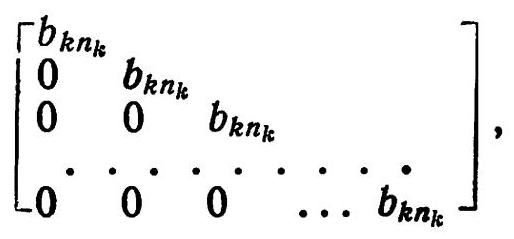
\includegraphics[max width=0.4\textwidth]{images/bo_d547k8bef24c73bgfcg0_100_547_926_514_239_0.jpg}
\end{center}
\hspace*{3em} 

у которой \({b}_{k{n}_{k}} \neq  0\) , a элементы под главной диагональю равны нулю. Заметим, что у вектора h последние п, элементов нули, и что

\[
{h}_{k - 1},{n}_{k - 1} = {\left( {\lambda }_{k - 1} - {\lambda }_{k}\right) }^{{n}_{k}}{b}_{k - 1},{n}_{k - 1} \neq  0.
\]

Тогда легко вычислитъ, что векторы-столбцы

\[
{\left( \bar{A} - {\lambda }_{1}I\right) }^{{n}_{1} - 1}{\left( \bar{A} - {\lambda }_{2}I\right) }^{{n}_{2}}\ldots {\left( \bar{A} - {\lambda }_{k}I\right) }^{{n}_{k}}\bar{b},\ldots ,\left( {\bar{A} - {\lambda }_{k}I}\right) \bar{b},\bar{b}
\]

образуют треугольную матрицу с ненулевыми диагональными эле- ментами

\[
{\left( {\lambda }_{1} - {\lambda }_{2}\right) }^{{n}_{2}}\cdots {\left( {\lambda }_{1} - {\lambda }_{k}\right) }^{{n}_{k}}{b}_{1{n}_{1}} \neq  0,\ldots ,{b}_{k{n}_{k}} \neq  0.
\]

Поскольку определитель такой треугольной матрицы не равен нулю, то

\[
\det \left\lbrack  {\bar{b},\bar{A}\bar{b},\ldots ,{\bar{A}}^{n - 1}\bar{b}}\right\rbrack   \neq  0.
\]

Так как й \(\overline{A} = {PA}{P}^{-1}\) и \(\overline{b} = \overline{B}c = {PBc}\) ,то находнм,что

\[
\det \left\lbrack  {{Bc},{ABc},{A}^{2}{Bc},\ldots ,{A}^{n - 1}{Bc}}\right\rbrack   \neq  0,
\]

так что система

\[
\left( {\mathcal{L}}_{1}\right)
\]

\[
\dot{x} = {Ax} + \left( {Bc}\right) u
\]

обладает свойствами управляемости при μ (t) с R1. Teopeма дока- зана.

B следующей теореме получена физически содержательная и с математической точки зрения удобная каноническая форма для управляемых процессов со скалярными управлениями.

Теорема 7. Аемономный линейный прочесс

\[
{x}^{\left( n\right) } + {a}_{1}{x}^{\left( n - 1\right) } + \ldots  + {a}_{n}x = u,\;u \in  {R}^{1}
\]

ихи соопвемспеуюияя линейная сиспема е фазовом проспраясгве

\[
{x}^{1} = {x}^{2}
\]

(D)
\[
{x}^{2} = {x}^{3}
\]

\[
{\dot{x}}^{n} =  - {a}_{n}{x}^{1} - {a}_{n - 1}{x}^{2} - \ldots  - {a}_{1}{x}^{n} + u
\]

обладают свойством управляемости. Любая обладающая свойством управляемости система в R" вида

(L)
\[
\dot{x} = {Ax} + {Bu}
\]

при управлениях и не в линейно эквивалентна системе вида Ф.

Доказательство. Легко проверить, что для матриц

\begin{center}
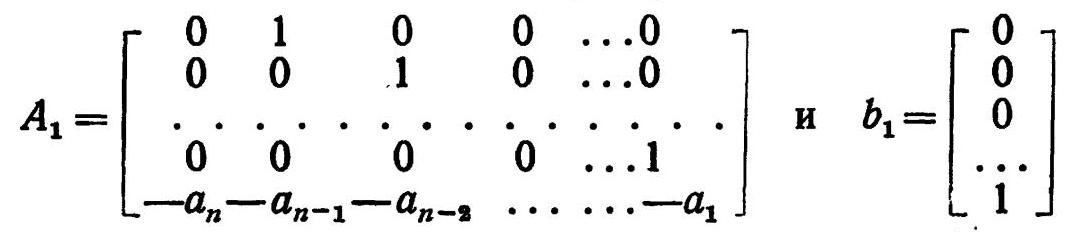
\includegraphics[max width=0.9\textwidth]{images/bo_d547k8bef24c73bgfcg0_101_255_981_1070_232_0.jpg}
\end{center}
\hspace*{3em} 

условия вполне управляемости теоремы 5 выполняются. Рассмот. рим теперь вполне управляемый процесс Ф. Определим действи- тельную невырожденную (n×n)-матрицу:

\[
P = \left\lbrack  {{A}^{n - 1}b,{A}^{n - 2}b,\ldots ,{A}^{2}b,{Ab},b}\right\rbrack  .
\]

Введем новые координаты в \({R}^{n}\) преобразованием \(\bar{x} = {P}^{-1}x\) ,так что система Q примет вид

\[
\bar{x} = {P}^{-1}{AP}\bar{x} + {P}^{-1}{bu}.
\]

Непосредственным перемноженнем матрнц проверяем, что

\[
b = \left\lbrack  {{A}^{n - 1}b,\ldots ,{Ab},b}\right\rbrack  \left[ \begin{array}{c} 0 \\  0 \\  \ldots \\  0 \\  1 \end{array} \right]  \text{ или }{P}^{-1}b = \left[ \begin{array}{c} 0 \\  0 \\  \ldots \\  0 \\  1 \end{array} \right]   = {b}_{1}
\]

\(\text{ и }{AP} = {PN}\) или \({P}^{-1}{AP} = N\) ,где

\[
N = \left[ \begin{array}{ccccc} {\alpha }_{1} & 1 & 0 & \ldots & 0 \\  {\alpha }_{2} & 0 & 1 & \ldots & 0 \\  \ldots & \ldots & \ldots & \ldots & \ldots \\  {\alpha }_{n - 1} & 0 & 0 & \ldots & 1 \\  {\alpha }_{n} & 0 & 0 & \ldots & 0 \end{array} \right]
\]

Постоянные \({\alpha }_{1},{\alpha }_{2},\ldots ,{\alpha }_{n}\) однозначно определяются из разложения

\[
{A}^{n}b = {\alpha }_{1}{A}^{n - 1}b + {\alpha }_{2}{A}^{n - 2}b + \ldots  + {\alpha }_{n}b.
\]

Для системы Ф характеристическое уравнение соответствующей матрицы \({A}_{1}\) имеет вид

\[
{A}_{1}^{n} =  - {a}_{1}{A}_{1}^{n - 1} - {a}_{2}{A}_{1}^{n - 2} - \ldots  - {a}_{n}I.
\]

Аналогично,применяя описанное выше преобразованне координат \(\kappa\) chcreme D, получим матрицы \(N\) и \(\left[ \begin{array}{c} 0 \\  0 \\  \ldots \\  1 \end{array} \right]\) ,если полилоложить- \({a}_{1} = \; = {\alpha }_{1}, - {a}_{2} = {\alpha }_{2},\ldots , - {a}_{n} = {\alpha }_{n}\) . Поэтому снстема \(\mathcal{L}\) линейно экви- валентна системе の. Теорема доказана.

В следствиях из теоремы 5 мы изучали области нуль-управ- ляемости ( для автономного линейного процесса \(\mathcal{L}\) в простран- стве R", причем управления удовлетворяли условию и (н) с Ω⊂C R". В следующей ниже теореме дается исчерпывающее описание того важного случая, когда область нуль-управляемости совпадает со всем пространством, т. е. когда можно, исходя из любой точки пространства, попасть в начало координат. Поскольку это будет уже не локальный, а глобальный анализ, то нам придется ввести некоторые предположения глобального характера относи- тельно \(\mathcal{L}\) и \(\Omega\) .

T e o p e ма 8. Рассмотрим автономную линейную систему в R":

\[
\left( \mathcal{L}\right)
\]

\[
\dot{x} = {Ax} + {bu},\;u \in  \Omega
\]

с компактным ограничивающим множеством Ω⊂R' содержащим точку и =0. Тогда область нуль-управляемости 6 совпадает с R", если и только если выполнены следующие условия:

(a) система Q обладает свойством управляемости;

(b) все собственные значения λ матрицы A удовлетворяют \(y < \lambda  < 0\) . [解] Re \(\lambda  \leq  0\) .

Доказательство. Если £ не обладает свойством управ- ляемости, то в соответствии со следствием 2 из теоремы 5 суще- ствуют точки пространства R", из которых нельзя попасть в на- чало координат.

Предположим, что матрица А системы Y имеет собственное значение \(\lambda\) c Re \(\lambda  > 0\) . Тогда существует вещественное невырож- денное преобразование координат в \({R}^{n},y = {Px}\) такое,что система 𝒳 принимает вид

\[
y = {PA}{P}^{-1}y + {Pbu},
\]

\[
{\dot{y}}^{1} = \lambda {y}^{1} + {b}_{1}u,\;\text{ если }\;\lambda  > 0,
\]

или

\[
{y}^{1} = \alpha {y}^{1} + \beta {y}^{2} + {b}_{1}u,\;{y}^{2} =  - \beta {y}^{1} + \alpha {y}^{2} + {b}_{2}u,
\]

если \(\lambda  = \alpha  + {i\beta }\) и \(\alpha  > 0\) . Выберем начальную точку \({y}_{0} \in  {R}^{n}\) так, чтобы у было очень большим положительным числом (или чтобы число уверхных доле меня большим, во втором случае). Тогда \(\frac{d{y}^{1}}{dt} > 0\;\left( {\text{ или }\frac{d}{dt}\left( {{y}^{{1}^{2}} + {y}^{{2}^{2}}}\right)  > 0\text{ при }t > 0}\right.\) и любом управлении и из множества Ω. Таким образом, из точки у нельзя попасть в на- чало координат под действием управления и (t) с Ω. Поэтому усло- вие € = kn влечет за собой выполнение условий (а) и (b).

Предположим теперь, что система 8 обладает свойством управ- ляемости и что для каждого собственного значения λ матрицы \(A\) выполняется условие Re \(\lambda  \leq  0\) . Покажем сначала, что можно ог- раничиться рассмотрением лишь случая, когда все собственные значения матрицы A чисто мнимые.

Можно считать, что система 8 линейным невырожденным пре- образованием координат в \({R}^{n}\) приведена к виду

\[
\left\lbrack  \begin{array}{l} {x}_{p} \\  {x}_{q} \end{array}\right\rbrack   = \left[ \begin{array}{cc} {A}_{p} & 0 \\  0 & {A}_{q} \end{array} \right]  \left\lbrack  \begin{array}{l} {x}_{p} \\  {x}_{q} \end{array}\right\rbrack   + \left\lbrack  \begin{array}{l} {b}_{p} \\  {b}_{q} \end{array}\right\rbrack  u,
\]

где каждое собственное значение λ, матрицы \({A}_{p}\) является чисто мнимым, а каждое собственное значение λ, матрицы А, удовлет- воряет неравенству Re \({\lambda }_{q} < 0.\Pi\) ри нулевом управлении \(u\left( t\right)  = 0\) решения асимптотически устойчивой системы

\[
{\dot{x}}_{q} = {A}_{q}{x}_{q}
\]

стремятся к хде 0 при t → + ∞. Далее, если координаты хар вы- браны соответствующим образом, то радиальная составляющая скорости будет отрицательна,

\[
{x}_{q}^{\prime }{x}_{q} = {x}_{q}^{\prime }{A}_{q}{x}_{q} \leq   - \zeta {x}_{q}^{\prime }{x}_{q}\;\text{ для }\;0 < \zeta  <  - \operatorname{Re}{\lambda }_{q},
\]

и если в дальнейшем использовать управления и(t) с достаточно малыми нормами, то решение хдо (б) будет оставаться внутри до- статочно малой окрестности \({N}_{q}\) точки \({x}_{q} = 0\) . Таким образом, если нам удастся, исходя из произвольной начальной точки, перевести обладающую свойством управляемости систему

\[
{\dot{x}}_{p} = {A}_{p}{x}_{p} + {b}_{p}u
\]

в достаточно малую окрестность \({N}_{n}\) точки \({x}_{n} = 0\) с помощью уп- равлений \(u\left( t\right)\) с достаточно малыми нормами \(\left| {u\left( t\right) }\right|\) , to тогда из свойства управляемости системы 8 будет следовать, что C = R". Поэтому можно свести нашу задачу к изучению такой вполне управляемой системы

\[
\dot{x} = {Ax} + {bu},
\]

где матрица А имеет лишь чисто мнимые собственные значения. Нам надо показать, что такая система может быть переведена из произвольной точки \({x}_{0} \in  {R}^{n}\) в некоторую заданную заранее ок- рестность \(N\) точки \(x = 0\) при помощи управления \(u\left( t\right)\) такого, что \(\left| {u\left( t\right) }\right|  < \varepsilon\) для заданного \(\varepsilon  > 0\) . Этим завершится доказа- тельство нашей теоремы.

В соответствии с теоремой 7, система 8 является линейно эквивалентной в \({R}^{n}\) системе Ф, определяемой следующим образом:

(D)
\[
{D}^{s}\left( {{D}^{2} + {\gamma }_{1}}\right) \left( {{D}^{2} + {\gamma }_{2}}\right) \ldots \left( {{D}^{2} + {\gamma }_{r}}\right) x = u,
\]

где \(s \geq  0,r \geq  0\) -порядки дифференцирования, \(\mathrm{a}{\gamma }_{1},\ldots ,{\gamma }_{r}\) - положительные постоянные; состояние системы определяется каж- дым из векторов \(\left( {x,x,\ldots ,{x}^{\left( n - 1\right) }}\right)\) или \(\left( {x,{x}^{\prime },\ldots ,{x}^{n - 1}}\right)\) .

Рассмотрим сначала случай \(r = 0,s \geq  1\) . Если \(s = 1\) ,то иско- мое управление легко построить (см. пример 1 главы 1). Более того, можно выбрать управление \(u\left( t\right)  \in  {C}^{\infty }\) на отрезке \({t}_{0} \leq  t \leq  {t}_{1}\) , переводящее систему из начальной точки х, в точку х, =0 ТАК, что

1) \(u\left( t\right)  = 0\) в некоторой окрестности концевых точек t=t, u \(t = {t}_{1}\)

2) \(x\left( t\right)  = 0\) в некоторой окрестности точки н1.

Эти ограничения накладываются на управления для того, что- бы можно было составить из них последовательность, сходящуюся к дифференцируемой функции. В оставшейся части доказатель- ства мы будем называть такие управления приемлемыми. Введем \(\sigma\) -норму для управлений из С \textdegree :

\[
{\left| u\left( t\right) \right| }_{\sigma } = \left| {u\left( t\right) }\right|  + \left| {\dot{u}\left( t\right) }\right|  + \ldots  + \left| {{u}^{\left( \sigma \right) }\left( t\right) }\right| ;
\]

построение приемлемого управления \(u\left( t\right)\) c \({\left| u\left( t\right) \right| }_{\sigma } \leq  \varepsilon\) для задан- ных σ ≥0 и ε > 0, переводящего систему Dx=u из произволь- ной начальной точки \({x}_{0}\) в точку \({x}_{1} = 0\) ,мы предоставляем читателю в качестве упражнения. Далее, считая, что такое приемлемое управление построено для системы Dx=u, применим математи- ческую индукцию, и будем считать, что существуют такие прием- лемые управления и для всех систем

\[
{D}^{j}x = u,\;j = 1,2,\ldots ,s - 1.
\]

Paccmorphm chстему]

\[
{D}^{s}x = u
\]

которую мы разложим на две системы \({D}^{s - 1}z = \xi\) и \({D\xi } = u\) . Пусть \(u\left( t\right)\) -некоторое управление из \({C}^{\infty }\) , a \({x}_{i}^{\prime }\left( t\right) ,\xi \left( t\right)\) и \(z\left( t\right)\) -coorber- ствующие ему решения с начальными условиями \({\xi }_{0} = {x}_{0}^{\left( s - 1\right) }\) и \({z}_{0} = {x}_{0},{z}_{0}^{\left( 1\right) } = {x}_{0}^{\left( 1\right) },\ldots ,{z}_{0}^{\left( s - 2\right) } = {x}_{0}^{\left( s - 2\right) }\) . Заметим,что \(z\left( t\right)  \equiv  x\left( t\right)\) .

Выберем сначала приемлемое управление и (t) на интервале \(0 \leq  t \leq  {t}_{1}\) c orраничением \({\left| u\left( t\right) \right| }_{a} < \varepsilon\) ,переводящее систему \({D\xi } = u\) из начального состояния \({\xi }_{0} = {x}_{0}^{\left( s - 1\right) }\) в конечное. состояние \({\xi }_{1} = 0\) . Это управление определяет также некоторое решение х(t) си- стемы D’s \(x = u\) ,и переводит систему из состояния ( \({x}_{0},{x}_{0}^{1},\ldots ,{x}_{0}^{s - 1}\) ) в некоторое состояние \(\left( {{x}_{1},{x}_{1}^{1},\ldots ,{x}_{1}^{s - 2},0}\right)\) . Пользуясь предполо- жением индукции, найдем допустимое управление ξ (t), определен- ное на интервале \({t}_{1} \leq  t \leq  {t}_{2}\) c orpaничением \({\left| \xi \left( t\right) \right| }_{\sigma  + 1} < \varepsilon\) , nepe- воляшее систему D5-1z=ξ из состояния (x, x1, ..., x1-2) в состояние \(\left( {0,0,\ldots ,0}\right)\) . Положим теперь \(u\left( t\right)  = {D\xi }\left( t\right)\) на интер- вале \({t}_{1} \leq  t \leq  {t}_{2}\) ; тогда и (t) будет приемлемым управлением на интер- вале 0 с t ≤ t, переводящим вектор \(x\left( t\right)\) из начального положе- ния \(\left( {{x}_{0},{x}_{0}^{1},\ldots ,{x}_{0}^{s - 1}}\right)\) в конечное положение \(\left( {0,0,\ldots ,0}\right)\) ,причем \({\left| u\left( t\right) \right| }_{\sigma } < \varepsilon\) . Итак, заключаем, что для системы

\[
{D}^{s}x = u,\;s \geq  1
\]

всегда существует приемлемое управление и(t), для которого \({\left| u\left( t\right) \right| }_{a} < \varepsilon\) ,переводящее ее из любой начальной точки в начало координат (σ ≥ 0, ε > 0—наперед заданные числа).

Теперь рассмотрим случай \(r \geq  1,s = 0\) ,так что система при- мет вид

\[
\left( {{D}^{2} + {\gamma }_{1}}\right) \left( {{D}^{2} + {\gamma }_{2}}\right) \ldots \left( {{D}^{2} + {\gamma }_{r}}\right) x = u.
\]

Для \(r = 1\) используем метод, изложенный в примере 1 (раздел 1.2) и следствие 1 из теоремы 5 (глава 2) для построения приемле- мого \{управления \(u\left( t\right)\) с ограничением \({\left| u\left( t\right) \right| }_{\sigma } < \varepsilon\) ,переводящего систему из заданного начального состояния в состояние покоя. Построение такого приемлемого управления мы вновь предлагаем в качестве упражнения. Пусть теперь r > 1, s = 0; снова приме- ним метод индукции.

Запишем систему Ф в виде

\[
\left( {{D}^{2} + {\gamma }_{2}}\right) \ldots \left( {{D}^{2} + {\gamma }_{r}}\right) z = \xi ,\;\left( {{D}^{2} + {\gamma }_{1}}\right) \xi  = u,
\]

и рассмотрим некоторое управление \(u\left( t\right)  \in  {C}^{\infty }\) и соответствующие ему решения \(x\left( t\right) ,z\left( t\right) ,\xi \left( t\right)\) с подходящими начальными условиями

\[
{z}_{0} = {x}_{0},\;{z}_{0}^{1} = {x}_{0}^{1},\ldots ,{z}_{0}^{{2r} - 3} = {x}_{0}^{{2r} - 3},
\]

\[
{\xi }_{0} = \left( {{D}^{2} + {\gamma }_{2}}\right) \ldots \left( {{D}^{2} + {\gamma }_{r}}\right) x\left( 0\right) ,{\xi }_{0}^{i} = \left( {{D}^{2} + {\gamma }_{2}}\right) \ldots \left( {{D}^{2} + {\gamma }_{r}}\right) {x}_{0}^{1}\left( 0\right) ,
\]

так что \(z\left( t\right)  = x\left( t\right)\) . Выберем сначала приемлемое управление и (t) на интервале 0 ≤ t ≤ t, с ограничением |u (t)|, < ε, переводящее систему (D*+y) ξ= \(u\) из положения ( \({\xi }_{0}\) , \({\xi }_{0}^{1}\) ) в положение (0,0). Это управление определяет решение \(x\left( t\right)\) системы Ф и переводит ee из состояния ( \({x}_{0},{x}_{0}^{1},\ldots ,{x}_{0}^{{2r} - 1}\) ) в некоторое состояние \(\left( {{x}_{1},{x}_{1}^{1},\ldots ,{x}_{1}^{{2r} - 1}}\right)\) . Используя предположение индукции, найдем приемлемое управление \(\xi \left( t\right)\) на интервале \({t}_{1} \leq  t \leq  {t}_{2}\) с ограниче- нием \({\left| \xi \left( t\right) \right| }_{\sigma  + 2} < \frac{\varepsilon }{1 + {\gamma }_{1}}\) ,переводящее вектор \(z\left( t\right)\) из начального положения \(\left( {{x}_{1},{x}_{1}^{1},\ldots ,{x}^{{2r} - 3}}\right)\) в положение \(\left( {0,0,\ldots ,0}\right)\) . Положим \(u\left( t\right)  = \left( {{D}^{2} + {\gamma }_{1}}\right) \xi \left( t\right)\) на интервале \({t}_{1} \leq  t \leq  {t}_{2}\) ; тогда \(u\left( t\right)\) . является приемлемым управлением на интервале О ≤ < t </t>, и переводит вектор \(x\left( t\right)\) из положения \(\left( {{x}_{0},{x}_{0}^{1},\ldots ,{x}_{0}^{{2r} - 1}}\right)\) в положение (0,0,…,0,0). Кроме того, \({\left| \xi \left( t\right) \right| }_{\sigma  + 2} + {\gamma }_{1}{\left| \xi \left( t\right) \right| }_{\sigma } < \varepsilon\) , OTKYJA cpa3y следует, что \({\left| u\left( t\right) \right| }_{\sigma } < \varepsilon\) . Таким образом, при любых ге 1, \(s = 0\) для системы Ф существует приемлемое управление \(u\left( t\right)\) .

Наконец, рассмотрим общий случай системы Ф для \(r \geq  1\) , \(s \geq  1\) . Здесь положим

\[
\left( {{D}^{2} + {\gamma }_{1}}\right) \ldots \left( {{D}^{2} + {\gamma }_{r}}\right) z = \xi ,\;{D}^{s}\xi  = u
\]

и используем подходящие начальные условия для заданного управ- ления \(u\left( t\right)  \in  {C}^{\infty }\) и соответствующих ему решений и (t), \(\xi \left( t\right) ,z\left( t\right)\) :

\[
{z}_{0} = {x}_{0},\;{z}_{0}^{1} = {x}_{0}^{1},\ldots ,{z}_{0}^{{2r} - 1} = {x}_{0}^{{2r} - 1},
\]

\[
{\xi }_{0} = \left( {{D}^{2} + {\gamma }_{1}}\right) \ldots \left( {{D}^{2} + {\gamma }_{r}}\right) x\left( 0\right) ,\ldots ,
\]

\[
{\xi }_{0}^{s - 1} = {D}^{s - 1}\left( {{D}^{2} + {\gamma }_{1}}\right) \ldots \left( {{D}^{2} + {\gamma }_{r}}\right) x\left( 0\right) ,
\]

так что \(z\left( t\right)  = x\left( t\right)\) . Сначала выберем приемлемое управление и (t) на интервале 0≤ \(t \leq  {t}_{1}\) с ограничением \({\left| u\left( t\right) \right| }_{\sigma } < \varepsilon\) ,переводящее вектор \(\xi \left( t\right)\) из положения \(\left( {{\xi }_{0},\ldots ,{\xi }_{0}^{s - 1}}\right)\) в конечное положение \(\left( {0,0,...,0}\right)\) . Это управление переводит конец вектора \(x\left( t\right)\) из точки \(\left( {{x}_{0},{x}_{0}^{1},\ldots ,{x}_{0}^{{2r} + s - 1}}\right)\) в некоторую точку \(\left( {{x}_{1},{x}_{1}^{1},\ldots ,{x}_{1}^{{2r} + s - 1}}\right)\) . Выберем ξ(t) в качестве приемлемого управления на интервале \({t}_{1} \leq  \bar{t} \leq  {t}_{2}\) ,переводящего вектор \(z\left( t\right)\) из положения \(\left( {{x}_{1},{x}_{1}^{1},\ldots ,{x}_{1}^{{2r} - 1}}\right)\) в положение (0, 0, ..., 0) и удовлетворяющего ограничению \({\left| \xi \left( t\right) \right| }_{\sigma  + s} < \varepsilon\) . Положим \(u\left( t\right)  = {D}^{s}\xi \left( t\right)\) на интервале \({t}_{1} \leq  t \leq  {t}_{2}\) . Тогда \(u\left( t\right)\) является приемлемым управлением на интервале \(0 \leq  t \leq  {t}_{2}\) c orpaничением \({\left| u\left( t\right) \right| }_{\sigma } < \varepsilon\) ,переводящим систему Ф из состояния \(\left( {{x}_{0},{x}_{0}^{1},\ldots ,{x}_{0}^{{2r} + s - 1}}\right)\) в состояние \(\left( {0,0,\ldots ,0}\right)\) . Теорема доказана для всех случаев.

Следствие. Рассмотрим автономную линейную систему в R":

(
\[
\mathcal{L}
\]
 )
\[
\dot{x} = {Ax} + {Bu}
\]

с компактным ограничивающим множеством Ω ⊂ R", содержащим точку и =0 внутри себя. Предположим, что никакие две жорда- новы клетки матрицы А не содержат одинаковых собственных значений матрицы А. Тогда область нуль-управляемости С сов- падает со всем пространством R" в том и только том случае, если выполнены следующие условия:

(a) система 2 обладает свойством управляемости;

(b) все собственные значения λ матрицы А удовлетворяют условию Re \(\lambda  \leq  0\) .

Доказательство. Если \(\mathfrak{C}\)=R", то доказательство теоремы проводится совершенно так же, как и в случае m=1. Обратно, если система 必 обладает свойством управляемости, и Re \(\lambda  \leq  0\) , то по теореме 6 мы можем заменить ограничивающее множество Ω некоторым компактным интервалом пространства R1, содержащим точку и =0. А тогда можно применить теорему 8, из которой следует, что \(\mathcal{C} = {R}^{n}\) .

Если система

(
\[
\mathcal{L}
\]
 )
\[
\dot{x} = {Ax} + {Bu}
\]

обладает свойством управляемости в R", то ее можно, исходя из произвольной начальной точки \({x}_{0}\) , перевести в нулевую точку за конечный промежуток времени с помощью некоторого управления \(u\left( t\right)  \subset  {R}^{m}\) . Поведение такой системы резко отличается от ее пове- дения в случае, когда B=0, т. к. тогда в силу устойчивости системы (все собственные значения λ матрицы \(A\) имеют Re \(\lambda  < 0\) ) все решения ее стремятся к началу координат при t/—+-∞.

Определение. Автономная линейная система в

(2)
\[
\dot{x} = {Ax} + {Bu}
\]

называется стабилизируемой, если существует такое линейно зави- сящее от \(x\) управление \(u = {Dx}\) ,что система

\[
\dot{x} = {Ax} + {BDx} = \left( {A + {BD}}\right) x
\]

устойчива,т.е.если найдется такая постоянная действительная \(m \times  n\) -matphila \(D\) ,чтодействительные части собственных значений матрицы \(A + {BD}\) отрицательны.

Если 오 и ダーлинейно эквивалентные системы, так что \(\overline{A} = {PA}{P}^{-1}\) и \(\overline{B} = {PB}\) ,и если \(\mathcal{L}\) -стабилизируемая система, то и система \(\overline{\mathcal{P}}\) будет стабилнзируемой.Действительно,если матрнца (A + BD) устойчива, то и матрица

\[
P\left( {A + {BD}}\right) {P}^{-1} = \bar{A} + \bar{B}\bar{D}\;\left( {\bar{D} = D{P}^{-1}}\right)
\]

также устойчива.

Teopeма 9. Рассмотрим автономную линейную систему в R"

(L)
\[
\dot{x} = {Ax} + {Bu}
\]

с управлением и (t) ⊂ R1. Если система 2 обладает свойством управляемости, то она стабилизируема.

Доказательство. По теореме 7 систему 8 можно заме- нить линейно эквивалентной системой вида

MM

\[
{x}^{\left( n\right) } + {a}_{1}{x}^{\left( n - 1\right) } + \ldots  + {a}_{n}x = u,
\]

\[
\dot{{x}^{1}} = {x}^{2},\;\dot{{x}^{2}} = {x}^{3},\ldots ,\dot{{x}^{n}} =  - {a}_{n}{x}^{1} - {a}_{n - 1}{x}^{2} - \ldots  - {a}_{1}{x}^{n} + u.
\]

ВОзьмем произвольный постоянный вектор

\[
D = \left( {{d}_{n},{d}_{n - 1},\ldots ,{d}_{1}}\right)
\]

и пусть

\[
u = {d}_{n}{x}^{1} + {d}_{n - 1}{x}^{2} + \ldots  + {d}_{1}{x}^{n}.
\]

Тогда наша снстема の становится снстемой собратной связыо:

\[
{x}^{\left( n\right) } + \left( {{a}_{1} - {d}_{1}}\right) {x}^{\left( n - 1\right) } + \cdots  + \left( {{a}_{n} - {d}_{n}}\right) x = 0.
\]

В частности, можно получить устойчивую систему, если выбрать вектор \(D\) таким образом,чтобы характеристический многочлен имел вид

\[
{\lambda }^{n} + \left( {{a}_{1} - {d}_{1}}\right) {\lambda }^{n - 1} + \cdots  + \left( {{a}_{n} - {d}_{n}}\right)  = {\left( \lambda  + 1\right) }^{n};
\]

это можно сделать, полагая

\[
{a}_{i} - {d}_{i} = \left( \begin{array}{c} n \\  i \end{array}\right) \;\mathrm{{\text{ п }\text{ р }\text{ и }}}\;1 \leq  i \leq  n.
\]

Теорема доказана.

В последних двух теоремах этого раздела мы вновь вернемся к общему случаю многомерных управлений и (t) с R*, m ≥1. Мы изучим здесь некоторые, не обладающие свойством управляе- мости, системы, пытаясь либо выделить из них части, обладаю- щие управляемостью, либо аппроксимировать системами, облада- ющими управляемостью.

T e o p e ма 10. Рассмотрим автономную линейную систему в R":

(L)
\[
\dot{x} = {Ax} + {Bu}.
\]

Существует единственное линейное подпространство C простран- ства R", такое, что

(a) \(C - u\) нвариантное подпространство для \(\mathcal{L}\) , m. e. каждая траектория системы, исходящая из точки, принадлежащей под- пространству C, целиком лежит в С и никакая траектория, начинающаяся вне C, не может привести в C.

(b) если рассматривать 2 только в подпространстве C, то си- стема Ф будет обладать свойством управляемости.

Доказательство. Пусть С-множество всех тех точек в \({R}^{n}\) ,в которые система может быть переведена из начала коор- динат за конечный промежуток времени с помощью управлений \(u\left( t\right)  \subset  {R}^{m}\) . Покажем сначала, что C является линейным простран- CTBOM.

Пусть \(0 < {t}_{1} < {t}_{2}\) ; рассмотрим точки C:

\[
{x}_{1}\left( {t}_{1}\right)  = {\int }_{0}^{{t}_{1}}{e}^{A\left( {{t}_{1} - s}\right) }B{u}_{1}\left( s\right) {ds}
\]

\[
{x}_{2}\left( {t}_{2}\right)  = {\int }_{0}^{{t}_{2}}{e}^{A\left( {{t}_{2} - s}\right) }B{u}_{2}\left( s\right) {ds}.
\]

В первом интеграле положим \(\sigma  = s + {t}_{2} - {t}_{1}\) и определим управ- ление следующим образом:

\[
{U}_{1}\left( \sigma \right)  = \left\{  \begin{array}{ll} 0 & \text{ на }0 \leq  t \leq  {t}_{2} - {t}_{1}, \\  {u}_{1}\left( {\sigma  - {t}_{2} + {t}_{1}}\right) & \text{ на }{t}_{2} - {t}_{1} < \sigma  \leq  {t}_{2}. \end{array}\right.
\]

Torja

\[
{x}_{1}\left( {t}_{1}\right)  = {\int }_{0}^{{t}_{2}}{e}^{A\left( {{t}_{2} - \sigma }\right) }B{U}_{1}\left( \sigma \right) {d\sigma }
\]

и, следовательно, точки и, кшен сд мси маше достичь из начала коорди- нат за время г. Таким образом, линейной комбинации управле- ний \({U}_{1}\left( t\right)\) и \({u}_{2}\left( t\right)\) на \(0 \leq  t \leq  {t}_{2}\) соответствует аналогичная линей- ная комбинация точек \({x}_{1}\left( {t}_{1}\right)\) и \({x}_{2}\left( {t}_{2}\right)\) . Cледовательно, \(C\) является линейным пространством.

Заметим, что множество С состоит из одной нулевой точки в том и только том случае, если 𝒳 полностью неуправляемая система, т. е. если \(B = 0\) . В этом случае теорема верна, поэтому условимся считать, что размерность к подпространства С строго больше нуля.

В силу конструкции пространства C никакая траектория си- стемы Z из \(C\) не выводит. Ясно, что существует система коор- динат \(\left( {{\bar{x}}^{1},\ldots ,{\bar{x}}^{n}}\right)\) в \({R}^{n}\) такая, что подпространство С в R задается уравнениями \({\bar{x}}^{k + 1} = 0,\ldots ,\overline{{x}^{n}} = 0\) , a система 𝒳 может быть записана в виде

\[
\begin{array}{l} {\dot{\bar{x}}}_{1} = {A}_{11}{\bar{x}}_{1} + {A}_{12}{\bar{x}}_{2} + {B}_{1}u, \\  {\dot{\bar{x}}}_{2} = {A}_{22}{\bar{x}}_{2}, \end{array}
\]

где

\[
{\bar{x}}_{1} = \left[ \begin{array}{c} {\bar{x}}^{1} \\  \vdots \\  {\bar{x}}^{k} \end{array} \right]  \;{\bar{x}}_{2} = \left[ \begin{array}{c} {\bar{x}}^{k + 1} \\  \vdots \\  {\bar{x}}^{n} \end{array} \right]  .
\]

Здесь мы использовали, что \({\dot{\bar{x}}}_{2} = 0\) на \(C\) . Заметим теперь,что ни- какая точка \(\bar{x} = \left( {{\bar{x}}_{1},{\bar{x}}_{2}}\right)\) ,для которой \({\bar{x}}_{2} \neq  0\) ,не может быть пере- ведена в C, следовательно C-инвариантное подпространство.

Будем теперь рассматривать систему 𝒳 лишь на С, т. е. положим

\[
\left( {\mathcal{L}}_{c}\right)
\]

\[
\dot{{\bar{x}}_{1}} = {A}_{11}{\bar{x}}_{1} + {B}_{1}u,\;{\bar{x}}_{2} = 0.
\]

Поскольку из начала координат можно попасть в любую точку С то на основании следствия 2 из теоремы 5 система Z, обладает свойством управляемости в С.

Пусть, наконец, C’ есть любое инвариантное линейное под- пространство в R", в котором система 8 обладает свойством управляемости. Поскольку \({C}^{\prime }\) инвариантно, то оно должно вклю- чать все точки, в которые можно попасть из начала координат, так что \(C \subset  {C}^{\prime }\) . Поскольку система 8 обладает свойством управ- ляемости в C’, то из каждой точки \({C}^{\prime }\) можно попасть в начало координат и, следовательно, \({C}^{\prime } \subset  C\) . Поэтому \({C}^{\prime } = C\) ,и мы дока- зали единственность подпространства C, удовлетворяющего усло- виям (а) и (b) нашей теоремы. Тем самым теорема полностью доказана.

Инвариантное подпространство С называется подпространст- вом управляемости для системы 8, а система Q\_6—вполне управ- ляемой частью системы Q.

Cледствие. Пусть C —подпространство управляемости для системы

(B)
\[
\dot{x} = {Ax} + {Bu}.
\]

Toгда существуют координаты х= \(\left\lbrack  \begin{array}{l} {\bar{x}}_{1} \\  {\bar{x}}_{2} \end{array}\right\rbrack\) в \({R}^{n}\) maкие, umo noд- пространство C определяется в R" уравнением х, =0, а система \(\mathcal{L}\) записывается в виде

\[
\dot{\overline{{x}_{1}}} = {A}_{11}\overline{{x}_{1}} + {A}_{12}\overline{{x}_{2}} + {B}_{1}u,
\]

\[
{\bar{x}}_{2} = {A}_{22}{\bar{x}}_{2}
\]

причем размерность подпространства C совпадает с рангом мат- рицы [B, AB, A'B, ..., A"-iB].

Доказательство. Доказывая теорему, мы установили су- шествование требуемых координат \(\bar{x} = \left\lbrack  \begin{array}{l} {\bar{x}}_{1} \\  {\bar{x}}_{2} \end{array}\right\rbrack\) . (Заметим, что \({\bar{x}}_{1} = 0\) , если \(C = 0\) ,т. е. если вер и £ полностью неуправляема.)

Поскольку система Z, обладает свойством управляемости в C, то

\[
\dim C = \operatorname{rank}\left\lbrack  {{B}_{1},{A}_{11}{B}_{1},{A}_{11}^{2}{B}_{1},\ldots ,{A}_{11}^{k - 1}{B}_{1}}\right\rbrack   = k.
\]

Кроме toro,

\[
\operatorname{rank}\left\lbrack  {{B}_{1},{A}_{11}{B}_{1},\ldots ,{A}_{11}^{k - 1}{B}_{1}}\right\rbrack   = \operatorname{rank}\left\lbrack  {{B}_{1},{A}_{11}{B}_{1},\ldots ,{A}_{11}^{n - 1}{B}_{1}}\right\rbrack  .
\]

Oднако

\[
{\bar{A}}^{l}\bar{B} = \left[ \begin{array}{cc} {A}_{11}^{l} & {B}_{1} \\  0 & \end{array} \right]  ,\;0 \leq  l \leq  n,
\]

где

\[
\bar{A} = \left[ \begin{array}{cc} {A}_{11} & {A}_{12} \\  0 & {A}_{22} \end{array} \right]  ,\;\bar{B} = \left[ \begin{array}{c} {B}_{1} \\  0 \end{array} \right]  .
\]

Поэтому

\[
\dim C = \operatorname{rank}\left\lbrack  {\bar{B},\bar{A}\bar{B},{\bar{A}}^{2}\bar{B},\ldots ,{\bar{A}}^{n - 1}\bar{B}}\right\rbrack
\]

и из инвариантности ранга матрицы управляемости относительно линейной эквивалентности следует утверждение следствия.

Теорема 11. Рассмотрим автономную линейную систему в R":

\[
\left( {\mathcal{L}}_{0}\right)
\]

\[
\dot{x} = {A}_{0}x + {B}_{0}u.
\]

Если система Ф. обладает свойством управляемости, то сущест- вует такое е по мою любая автономная линейная система

\(\left( \mathcal{L}\right) \;x = {Ax} + {Bu},{\lambda Ax}\) п ри одиру пира \(\left| {A - {A}_{0}}\right|  < {\varepsilon }_{1},\left| {B - {B}_{0}}\right|  < {\varepsilon }_{1}\)

будет также обладать свойством управляемости.

Если система Q не является вполне управляемой, то для любого в > 0 существует обладающая свойством управляемости cucmema

\[
\left( {\mathcal{L}}_{1}\right) \dot{x} = {A}_{1}x + {B}_{1}u,\max {ax},{umo}\left| {{A}_{1} - {A}_{0}}\right|  < \varepsilon ,\left| {{B}_{1} - {B}_{0}}\right|  < \varepsilon .
\]

Такци образом, миожес𝚖ео облаdaючих сеойсмвом управляемосми cucmem omкрымо u всюòy плопино в иеmpчиском проспраисгиве seex agmonomiblx numewhor cucmem e \({R}^{n}\) , 2de paccmonine menody cucmeмами onpeðеляемся no формуле \(\left| {{A}_{1} - {A}_{0}}\right|  + \left| {{B}_{1} - {B}_{0}}\right|\) .

Доказательство.Если система \({\mathcal{L}}_{0}\) обладает свойством управляемости в \({R}^{n}\) ,то строки матрнцы \(\left\lbrack  {{B}_{0},{A}_{0}{B}_{0},\ldots ,{A}_{0}^{n - 1}{B}_{0}}\right\rbrack\) образуют систему из л линейно независимых векторов в про- странстве R"m. Если |A-льц с 8 и 1 B-B, 1 E 1, 1 B-B, 1 св 2 я для доста- точно малого в 1,0, должны аппроксимировать эти п векторов, и поэтому также должны быть линейно независимыми. Но тогда система

(
\[
\mathcal{L}
\]
 )
\[
\dot{x} = {Ax} + {Bu}
\]

также будет вполне управляемой.

C другой стороны, предположим, что система 8, не является вполне управляемой. Для заданного ε>0 выберем такие мат- рицы \({A}_{1}\) и \({B}_{1}\) ,чтобы \(\left| {{A}_{1} - {A}_{0}}\right|  < \varepsilon ,\left| {{B}_{1} - {B}_{0}}\right|  < \varepsilon\) и чтобы элементы матриц \({A}_{1}\) и \({B}_{1}\) были алгебраически независимы над полем ра- циональных чисел (т. е. чтобы не существовало полиномиальной (имеется в виду полином с рациональными коэффициентами) связи между элементами матриц А1 и В1-существование таких мат- риц А1 и В1 есть стандартное свойство арифметики веществен- ных чисел). Тогда

\[
\operatorname{rank}\left\lbrack  {{B}_{1},{A}_{1}{B}_{1},\ldots ,{A}_{1}^{n - 1}{B}_{1}}\right\rbrack   = n,
\]

поскольку ни один из (n×n)-миноров матрицы не может рав- няться нулю, так как каждый из них представляет собой многочлен от элементов матриц А1 и В1. Следовательно, систе- ма \({\mathcal{L}}_{1}\) обладает свойством управляемости. Теорема доказана.

Несмотря на некоторую искусственность построений при до- казательстве теоремы 11, она имеет важный физический смысл. Из нее следует, что, вообще говоря, произвольно взятая авто- номная линейная система 8 скорее всего будет обладать свой- ством управляемости, т. е. управляемость является типичным свойством автономной линейной системы. В частности, для описа- ния реальной физической системы с приближенно известными параметрами всегда можно подобрать вполне управляемую си- стему Ф. Однако иногда время, требуемое для приведения так подобранной системы в желаемое состояние, может быть столь велико, что выгоднее в качестве математической модели исполь- зовать систему gp, не обладающую свойством управляемости.

\section*{Упражнения}

1. Для системы Xe и, стограничением | и (t) | < ! вычислить и изобразить множество достижимости \(K\left( {t}_{1}\right)\) для \({t}_{1} = 1\) и \({t}_{1} = 2\) с начальным положением \({x}_{0} = 0,{\dot{x}}_{0} = 0;\mathrm{c}\) начальным положением \({x}_{0} = 0,{\dot{x}}_{0} = 4\) .

Указан и е: использовать теорему 2 и пример 2 главы 1.

2. Рассмотрите линейную систему в \({R}^{n}\) :

(L)
\[
\dot{x} = A\left( t\right) x + B\left( t\right) u + v\left( t\right)
\]

с компактным ограничивающим множеством \(\Omega  \subset  {R}^{m}\) и начальной точкой х, в момент \({t}_{0}\) . Точка РЕЭИ ( \({t}_{1}\) ) называется вершиной множества K (1,), если через нее проходит несколько гиперплоскостей, опорных для \(K\left( {t}_{1}\right)\) . Пока- жите, что если точка \(x\left( {t}_{1}\right)  = P\) является вершиной множества K(t1), то точка \(x\left( \tau \right)\) будет вершиной множества \(K\left( \tau \right)\) для всех т таких, что \({t}_{0} < \tau  \leq  {t}_{1}\)

3. Рассмотрите автономную линейную систему

\[
{x}^{\left( n\right) } + {a}_{1}{x}^{\left( n - 1\right) } + \ldots  + {a}_{n}x = {\beta }_{m}{u}^{\left( m\right) } + \ldots  + {\beta }_{0}u,{\beta }_{m} \neq  0.
\]

Покажнте,что е можно из любого начального состояния \(\left( {{x}_{0},{\dot{x}}_{0},\ldots ,{x}_{0}{}^{\left( n - 1\right) }}\right)\) перевести в состоянне \(\left( {0,0,0,\ldots ,0}\right)\) законечное время спомощьо управ- ления \(u\left( t\right)  \in  {C}^{m}\) .

4. Paccmorphm abtohomhyio линейную снстему в \({R}^{n}\) :

(x)
\[
\dot{x} = {Ax} + {Bu}
\]

с ограничивающим множеством Ω⊂\_ℵ", содержащим точку и = 0.

(a) Покажите, что \(K\left( {t}_{1}\right)  \subset  K\left( {t}_{2}\right)\) для \(0 < {t}_{1} < {t}_{2}\) , если в качестве началь- ной точки принять \({x}_{0} = 0\) . [Указани е: см. теорему 10.]

(b) Покажите, что если множество Ω выпукло и имеет непустую внутрен- ность, то внутренность множества K (t, c) сдержится в K∞ (t, ). Здесь под \({K}_{\infty }\left( {t}_{1}\right)\) понимается множество достижимости для исходной точки х, и управ- лений и (t) \(\in  {C}_{\infty }\) в Ω. [Указани е: управление и (t) ⊂Ω можно слабо ап- проксимировать управлением из \({C}^{\infty }\) ,лежащим внутри Ω.]

5. Для каких значений действительного параметра ρ система

\[
\left\lbrack  \begin{array}{l} {\dot{x}}_{1}^{1} \\  {\dot{x}}^{2} \end{array}\right\rbrack   = \left\lbrack  \begin{array}{r} {2\rho } - 3 \\  0 \end{array}\right\rbrack  \left\lbrack  \begin{array}{l} {x}^{1} \\  {x}^{2} \end{array}\right\rbrack   + \left[ \begin{array}{cc} 1 & 1 \\  {\rho }^{2} - \rho & 0 \end{array} \right]  \left\lbrack  \begin{array}{l} {u}^{1} \\  {u}^{2} \end{array}\right\rbrack
\]

будет обладать свойством управляемости? Для каких р эту систему можно свести к обладающей свойством управляемости системе со скалярным управ- лением?

6. Рассмотрим автономную линейную систему в R":

(L)
\[
\dot{x} = {Ax} + {Bu},\;u \in  {R}^{m}.
\]

Если существует такой ненулевой \(m\) -мерный вектор \(w\) ,что векторы

\[
{Bw},{ABw},{A}^{2}{Bw},\ldots ,{A}^{n - 1}{Bw}
\]

линейно независимы, то система £ обладает свойством управляемости. Дока- жите это утверждение и приведите пример, показывающий, что обратное утверждение неверно.

7. Рассмотрим автономную линейную систему в R":

(L)
\[
\dot{x} = {Ax} + {bu},\;u \in  {R}^{1}.
\]

Пусть \(\bar{A} = \operatorname{diag}\left\{  {{A}_{1},{A}_{2},\ldots ,{A}_{k}}\right\}   -\) каноническая жорданова форма мат- рицы A, и пусть

\[
\bar{b} = \left[ \begin{array}{c} {b}_{11} \\  \cdots \\  {b}_{1{n}_{1}} \\  \cdots \end{array} \right]
\]

— соответствующий вектор \(b\) ,записанный,как в теореме 6. Докажите, что система £ обладает свойством управляемости тогда и только тогда, когда выполняются следующие два условия:

(a) никакие две клетки \({A}_{{k}_{1}}\) и \({A}_{{k}_{2}}\) не имеют одинаковых собственных значений;

(b)
\[
{b}_{1{n}_{1}} \neq  0,\;{b}_{2{n}_{2}} \neq  0,\ldots ,{b}_{k{n}_{k}} \neq  0.
\]

8. В задаче Лурье—Летова из теории автоматического регулирования рассматривается линейная система в

(L)
\[
\dot{x} = {Ax} + {bu}
\]

с матрицей \(A = \operatorname{diag}\left\{  {{\lambda }_{1},{\lambda }_{2},\ldots ,{\lambda }_{k}}\right\}\) ,где все собственные значения \({\lambda }_{i}\) pas- личны. Покажите, что система 𝒳 линейно эквивалентна линейной системе 𝒳 с матрицей \(\bar{A} = A\) и матрицей

\[
\bar{b} = \left[ \begin{array}{c} 1 \\  1 \\  \cdots \\  1 \end{array} \right]
\]

в том и только том случае, если система £ обладает свойством управляе- MOCTH.

9. В критерии устойчивости Payca — Гурвица утверждается, что каждый корень λ действительного многочлена

\[
{\lambda }^{n} + {a}_{1}{\lambda }^{n - 1} + \ldots  + {a}_{n} = 0
\]

имеет отрнцательную вещественную часть толькотогда,когда \({D}_{k} > 0\) , \(k = 1,2,\ldots\) 3 десь

\[
{D}_{1} = {a}_{1},\;{D}_{2} = \left| \begin{array}{cc} {a}_{1} & {a}_{3} \\  1 & {a}_{2} \end{array}\right| ,\ldots ,{D}_{k} = \left| \begin{array}{ccccc} {a}_{1} & {a}_{3} & {a}_{5} & \ldots & {a}_{{2k} - 1} \\  1 & {a}_{2} & {a}_{4} & \ldots & {a}_{{2k} - 2} \\  0 & {a}_{1} & {a}_{3} & \ldots & {a}_{{2k} - 3} \\  0 & 1 & {a}_{2} & \ldots & {a}_{{2k} - 4} \\  0 & 0 & {a}_{1} & \ldots & {a}_{{2k} - 5} \\   & \ldots & \ldots & \ldots & \ldots \\  0 & 0 & 0 & \ldots & {a}_{k} \end{array}\right| ,
\]

где \({a}_{k} \geq  0\) .

(a) Покажите, что если Re \(\lambda  \leq  0\) для всех корней \(\lambda\) ,то \({a}_{k} \geq  0\) и \({D}_{k} \geq  0\) для \(k = 1,2,\ldots ,n\) .

(b) Покажите, что если \({a}_{k} \geq  0\) и \({D}_{k} \geq  0\) для \(k = 1,\ldots ,n\) ,то при \(n \leq  3\) все корни λ имеют отрицательную вещественную часть. Пример \({\lambda }^{4} + {\lambda }^{2} + 1 = 0\) показывает, что это утверждение неверно при \(n = 4\) .

10. Покажите, что системы

\[
{Dx} = u\;\text{ и }\;\left( {{D}^{2} + 1}\right) x = u
\]

обладают приемлемыми управлениями и (t) (в смысле теоремы 8), удовлетво- ряющими ограничению \(\lceil u\left( t\right) \rceil  < \varepsilon\) , которые переводят их из произвольной начальной точки в начало координат.

11. Покажите, что автономные линейные системы

\[
\left( \mathcal{L}\right)
\]

\[
\dot{x} = {Ax} + {Bu},
\]

обладающие свойством управляемости относительно скаля рных управлений 1) являются типичными в смысле теоремы 11.

12. Автономная линейная система в \({R}^{n}\)

(L)
\[
\dot{x} = {Ax} + {bu},\;u \in  {R}^{1}
\]

называется управляемой со сколь угодно малым управлением, если для любого в > 0 и любых двух точек х, и х нз пс уществует управление \(u\left( t\right)\) , удовлетворяющее ограничению | и (i) | ≤ e, которое переводит систему из состояния \({x}_{0}\) в состояние х за конечный промежуток времени. Покажите, что система £ будет управляемой со сколь угодно малым управлением в том и только том случае, если

4 (a) \(\mathcal{L}\) обладает свойством управляемости;

(b) каждое собственное значение λ матрицы A является чисто мнимым. 13. Система из двух сцепленных пружин совершает в горизонтальной плоскости колебательное движение около положения равновесия. (Трение отсутствует.) Уравнения движения имеют вид

\[
\ddot{x} =  - {k}_{1}x + {k}_{2}\left( {y - x}\right) ,\;\ddot{y} =  - {k}_{2}\left( {y - x}\right)  + u,
\]

где х и у —отклонения свободных концов от их положений равновесия, к1 > 0 и \({k}_{2} > 0 -\) коэффициенты жесткости пружин, а и (t) — управляющая сила, приложенная к концу второй пружины. Покажите, что такая система является управляемой со сколь угодно малым управлением (считать что движение происходит вблизи положения равновесия \(x = \dot{x} = 0,y = \dot{y} = 0\) ).

14. Рассмотрим автономную линейную систему в \({R}^{n}\) :

(x)
\[
\dot{x} = {Ax} + {Bu}
\]

с начальным положением х, в момент где о и с компактным ограничивающим множеством Ω. В предположении, что система £ обладает свойством управ- ляемости, множество H(Ω) имеет непустую внутренность в R*, а ранг мат- рицы B равен \(m\) , покажите, что компактное подмножество \(Z \subset  \Omega\) обладает свойством «релейности», т. е.

\[
{K}_{Z}\left( {t}_{1}\right)  \equiv  {K}_{\Omega }\left( {t}_{1}\right) \;\text{ для всех }\;{t}_{1} \geq  0
\]

\HRule

1) Cм. теорему 6. (Прим. ред.)

\HRule

тогда и только тогда, когда

\[
H\left( Z\right)  = H\left( \Omega \right)
\]

IУказание: в теореме 4 утверждается, что из условия \(H\left( Z\right)  = H\left( \Omega \right)\) следует наличие у множества Z свойства «релейности». Для доказательства обратного утверждения предположим, что \(H\left( Z\right)  \neq  H\left( \Omega \right)\) и рассмотрим опорную гипер- плоскость я к H(Ω), не пересекающую множества H(Z). Пусть у П В- внешняя единичная нормаль к плоскости я при некотором η1. Возьмем точку \({P}_{0} \in  \partial {K}_{\Omega }\left( {t}_{1}\right)\) ,в которой внешняя нормаль совпадает с \({\eta }_{1}\) . Это возможно,так как \({K}_{\Omega } = {K}_{H\left( \Omega \right) }\) есть выпуклое тело и ранг матрицы \(B\) равен m. Тогда лю- бое управление \({u}_{0}\left( t\right)  \subset  H\left( \Omega \right)\) ,переводящее систему из точки х,в о точку Ро, должно удовлетворять принципу максимума, а отсюда следует, что управле- ние \({u}_{0}\left( t\right)\) находится вне множества \(H\left( Z\right)\) для всех t,близких к t,1.

15. Пусть система x= Ax+bu oбладает свойством управляемости, как в теореме 9. Покажите, что управление и = Dx можно выбрать таким обра- зом, чтобы собственные значения матрицы A+bD равнялись заранее задан- ным величинам (однако таким, чтобы матрица А+bD оставалась действи- тельной).

\section*{2.4. Управляемость и наблюдаемость}

Рассмотрим действительную автономную линейную систему

(Y)
\[
\dot{x} = {Ax} + {Bu},
\]

где \(u \in  {R}^{m}\) -входной сигнал, или вектор управления, а хеке" решение, или вектор состояния системы. Может случиться, что лишь некоторые из составляющих вектора состояния или линей- ная комбинация его компонент имеют физический смысл, или вообще наблюдаемы. В этом случае описание системы дополняется уравнением наблюдения

(6)
\[
\omega  = {Hx}\text{ . }
\]

Здесь И — действительная постоянная (r×n)-матрица, определяю- щая наблюдаемый выход системы—r-мерный вектор ω, завися- щий от n-мерного вектора состояния х. Совокупность уравне- ний Z и б, полностью описывающая зависимость выхода от входа, называется автономной линейной наблюдаемой системой.

Пример. Рассмотрим систему

\[
{x}^{\left( n\right) } + {a}_{1}{x}^{\left( n - 1\right) } + \ldots  + {a}_{n}x = u,
\]

в которой наблюдаемым является лишь сам выход, но не его производные. Чтобы описать соответствующий процесс наблюдения,

надо к системе уравнений

\[
\left[ \begin{array}{c} {\dot{x}}^{1} \\  {\dot{x}}^{2} \\  \vdots \\  {\dot{x}}^{n} \end{array} \right]   = \left[ \begin{array}{cccccc} 0 & 1 & 0 & 0 & \ldots & 0 \\  0 & 0 & 1 & 0 & \ldots & 0 \\  \vdots & & & & & \\  0 & 0 & 0 & 0 & \ldots & 1 \\   - {a}_{n} &  - {a}_{n - 1} & & & \ldots &  - {a}_{1} \end{array} \right]  \left[ \begin{array}{c} {x}^{1} \\  {x}^{2} \\  \vdots \\  \vdots \\  {x}^{n} \end{array} \right]   + \left[ \begin{array}{c} 0 \\  0 \\  \vdots \\  0 \\  1 \end{array} \right]
\]

добавить уравнение

\[
\omega  = \left\lbrack  \begin{array}{llll} 1 & 0 & \ldots & 0 \end{array}\right\rbrack  \left[ \begin{array}{c} {x}^{1} \\  {x}^{2} \\  \vdots \\  {x}^{n} \end{array} \right]
\]

Пля линейной наблюдаемой системы

\[
\dot{x} = {Ax} + {Bu},\omega  = {Hx}
\]

зависнмрсть между входом и выходом даегся формулой

\[
\omega \left( t\right)  = H{e}^{At}{\int }_{0}^{t}{e}^{-{As}}{Bu}\left( s\right) {ds}
\]

при начальных условиях х, не на Если все составляющие вектора управления, кроме и у мены нулю, т. е.

\[
u\left( t\right)  = \frac{1}{\varepsilon }\left[ \begin{array}{c} 0 \\  \vdots \\  0 \\  1 \\  0 \\  \vdots \\  0 \end{array} \right]   = \frac{1}{\varepsilon }{e}_{j}\text{ на интервале 0 ≤ }t \leq  \varepsilon
\]

ТО

\[
\omega \left( t\right)  = H{e}^{At}\frac{1}{\varepsilon }{\int }_{0}^{\varepsilon }{e}^{-{As}}B{e}_{j}{ds}\;\text{ при }\;t \geq  \varepsilon  > 0.
\]

B предельном случае, при ε → 0, данная формула определяет решение, соответствующее единичному импульсу на входе системы, т. е. сигналу \(u\left( t\right)  = \delta \left( t\right) {e}_{j}\left( {\delta \left( t\right)  - }\right.\) функцию можно представить как некоторую идеализацию ступенчатой функции, или, точнее, как некоторую меру с весом +1, сосредоточенную в точке t=0). В пределе решение примет вид

\[
\omega \left( t\right)  = H{e}^{At}B{e}_{j}\;\pi \mathrm{p}\mathrm{u}\;t \geq  0.
\]

Иначе говоря, элемент \(\left( {i,j}\right)\) -матрицы

\[
W\left( t\right)  = H{e}^{At}B\;\mathrm{{\text{ п }\text{ р }\text{ и }}}\;t \geq  0
\]

дает составляющую \({\omega }^{i}\left( t\right)\) peшения \(\omega \left( t\right)\) , соответствующего импульс- ному сигналу и (t) = δ (t) e, Marpицей W (t) полностью опреде- ляются все связи между входом и выходом наблюдаемой системы. Действительно, для произвольного управления и (t) имеем

\[
\omega \left( t\right)  = {\int }_{0}^{t}W\left( {t - s}\right) u\left( s\right) {ds}\;{\text{ п }\text{ р }\text{ и }}\;t \geq  0,
\]

где \({x}_{0} = 0\) при \(t = 0\) .

Поскольку соотношение между \(u\left( t\right)\) и ω (t) имеет вид свертки, то удобно применить преобразование Лапласа к функциям \(u\left( t\right)\) и о (t). Обозначая их изображения через U (p) и Ω (p), по- лучим матричную передаточную функцию

\[
Z\left( p\right)  = L\left( {W\left( t\right) }\right)  = {\int }_{0}^{\infty }W\left( t\right) {e}^{-{pt}}{dt}
\]

Тогдасоотношение,связывающеевходсвыходомснстемы,приметвид

\[
\Omega \left( p\right)  = Z\left( p\right) U\left( p\right) .
\]

Определение. Для автономной линейной наблюдаемой си- CTEMbI(L)

\[
\dot{x} = {Ax} + {Bu},\;\omega  = H\left( x\right)
\]

матрица

\[
W\left( t\right)  = \left\{  \begin{array}{cc} H{e}^{At}B & \operatorname{\text{ п }\text{ р }\text{ и }}t \geq  0, \\  0 & \operatorname{\text{ п }\text{ р }\text{ и }}t < 0 \end{array}\right.
\]

называется импульсно-переходной матрицей, или весовой матрич- ной функцией.

Матрица, определяющая зависимость выхода от входа,

\[
Z\left( p\right)  = L\left( {W\left( t\right) }\right)  = {\int }_{0}^{\infty }W\left( t\right) {e}^{-{pt}}{dt}
\]

называется матричной передаточной функцией системы.

В этом разделе мы убедимся, что весовая функция, так же как и передаточная функция, полностью характеризует все ас- пекты задачи наблюдения. В основной теореме 14 дается строгое оказательство точного соответствия между матрицами вида Z(p) и процессами наблюдения. Сначала мы исследуем, какие из мат- риц Z (р) могут служить передаточными функциями; затем выде- лим два важных для приложений класса линейных процессов, а именно: класс вполне управляемых процессов, и класс вполне наблюдаемых процессов, а затем покажем, что эти классы в опреде- ленном смысле двойственны друг другу.

В силу известных свойств матрицы ей для постоянной (л х л)-мат- рицы A можно заключить, что Не \({e}^{At}B\) представляет собой (r × m)-мат- рицу с элементами вида \({t}^{\sigma }{e}^{\alpha t}\cos {\beta t}\) или \({t}^{\sigma }{e}^{\alpha t}\sin {\beta t}\left( {\sigma  = 0,1,2,3,\ldots }\right)\) и действительными α, β, или конечными линейными комбинациями таких членов. Назовем такие (r×m)-матрицы экспоненциально- полиномиальными матрицами.

Teopeма 12. Действительная r × m-матрица

\[
W\left( t\right)  = \left\{  \begin{array}{ccc} {W}_{0}\left( t\right) & {при} & t \geq  0, \\  0 & {при} & t < 0 \end{array}\right.
\]

является матричной весовой функцией для некоторого действи- тельного автономного линейного наблюдаемого процесса в том и только том случае, если W 0(t) является экспоненциально-полино- миальной матрицей.

Далее, (r×m)-матрица Z(p) есть матричная передаточная функция для некоторой действительной автономной линейной наблюдаемой системы в том и только том случае, если каждый элемент матрицы Z (р) является действительной дробно-рациональ- ной функцией от p, степень числителя которой меньше степени знаменателя.

Доказательство. Применяя элементарные формулы для преобразования Лапласа

\[
L\left( {{t}^{\sigma }{e}^{\alpha t}\cos {\beta t}}\right)  = {\left( -1\right) }^{\sigma }\frac{{d}^{\sigma }}{d{p}^{\sigma }}\left\lbrack  \frac{p - \alpha }{{\left( p - \alpha \right) }^{2} + {\beta }^{2}}\right\rbrack  ,
\]

\[
L\left( {{t}^{\sigma }{e}^{\alpha t}\sin {\beta t}}\right)  = {\left( -1\right) }^{\sigma }\frac{{d}^{\sigma }}{d{p}^{\sigma }}\left\lbrack  \frac{\beta }{{\left( p - \alpha \right) }^{2} + {\beta }^{2}}\right\rbrack
\]

и обратные формулы

\[
{L}^{-1}\left( \frac{1}{p}\right)  = 1
\]

\[
{L}^{-1}\left( \frac{p?}{{\left( p - a\right) }^{\sigma }}\right)  = \frac{d\rho }{dt\rho }\left\lbrack  {\frac{{t}^{\sigma  - 1}}{\left( {\sigma  - 1}\right) !}{e}^{at}}\right\rbrack  \text{ для }\sigma  \geq  1,0 \leq  \rho  < \sigma ,
\]

а также правила разложения на элементарные дроби, получаем, что \({W}_{0}\left( t\right)\) будет экспоненциально-полиномиальной матрицей тогда и только тогда, когда все элементы матрицы \(Z\left( p\right)\) являются дроб- но-рациональными функциями, у которых степень числителя меньше степени знаменателя. Таким образом надо доказать лишь первую часть теоремы.

Поскольку весовая матрица для любой действительной авто- номной наблюдаемой системы имеет вид Не \({e}^{At}B\left( {t \geq  0}\right)\) , то матрица \({W}_{0}\left( t\right)\) и ее преобразование Лапласа \(Z\left( p\right)\) должны иметь вид, указанный в теореме.

Пусть теперь \({W}_{0}\left( t\right)\) есть экспоненциально-полиномиальная матрица. Для доказательства теоремы мы должны построить автономную наблюдаемую систему, весовая функция которой вы- ражается через \({W}_{0}\left( t\right)\) , kax указано в теореме.

Пусть \({W}_{0}\left( t\right)  = \left( {{l}_{ij}\left( t\right) }\right)\) ,где \({l}_{ij}\left( t\right) ,1 \leq  i \leq  r,1 \leq  j \leq  m\) , \(\Pi\) per- ставляет собой конечную линейную комбинацию членов вида \({t}^{\sigma }{e}^{\alpha t}\cos {\beta t}\) и \({t}^{\sigma }{e}^{\alpha t}\sin {\beta t}\) . Каждый элемент \({l}_{ij}\left( t\right)\) является решением некоторого однородного линейного дифференциального уравнения с постоянными коэффициентами, например уравнения некоторого достаточно высокого порядка \(N\) . Следовательно, каждая из функ- ций \({l}_{ij}\left( t\right)\) представляет собой элемент фундаментальной (N X N)-мат- рицы решений е \({e}^{{A}_{ij}t}{C}_{ij}\) ,и если выбрать постоянные матрицы \({A}_{ij}\) и \({C}_{ij}\) соответствующим образом, то элемент l/i/() будет стоять в левом верхнем углу.

Построим теперь систему дифференциальных уравнений по- рядка Nrm,

\[
\dot{x} = {Ax},
\]

где

\[
A = \operatorname{diag}\left\{  {{A}_{11},{A}_{12},\ldots ,{A}_{1m},{A}_{21},\ldots ,{A}_{2m},\ldots ,{A}_{r1},\ldots ,{A}_{rm}}\right\}  .
\]

Положим

\[
C = \operatorname{diag}\left\{  {{C}_{11},\ldots ,{C}_{1m},\ldots ,{C}_{r1},\ldots ,{C}_{rm}}\right\}
\]

и рассмотрнм матрнцу

\[
{e}^{At}C = \operatorname{diag}\left\{  {{e}_{z - }^{{A}_{11}t}{C}_{11},\ldots ,{e}^{{A}_{rm}t}{C}_{rm}}\right\}  ,
\]

содержащую каждый из элементов l/j(t) в верхнем левом углу соответствующей клетки \({e}^{{A}_{ij}t}{C}_{ij}\) . Теперь остается выбрать постоян- ные матрицы \(H\) и \({B}_{1}\) так,чтобы имело место равенство

\[
{W}_{0}\left( t\right)  = H{e}^{At}C{B}_{1} = H{e}^{At}B.
\]

В качестве таковых можно взять, например, матрицы, состоя- щие из 0 и 1, расположенных определенным образом. Так, для случая \(r = 2,m = 3\) надо взять

\[
H = \left( \begin{array}{llllllllllllllllll} {10} & \ldots & 0 & {10} & \ldots & 0 & {10} & \ldots & 0 & {10} & \ldots & 0 & {10} & \ldots & 0 & {10} & \ldots & 0 \\  {00} & \ldots & 0 & {00} & \ldots & 0 & {00} & \ldots & 0 & {10} & \ldots & 0 & {10} & \ldots & 0 & {10} & \ldots & 0 \end{array}\right) ,
\]

ТАК, ЧТО

\[
H{e}^{At}C = \left( \begin{array}{cccccccccc} {l}_{11} * \ldots  * & {l}_{12} * \ldots  * & {l}_{13} * \ldots  * & 0 & \ldots & 0 & 0 & \ldots & 0 & 0 \\  0 & \ldots & 0 & 0 & \ldots & 0 & {l}_{21} * \ldots  * & {l}_{22} * \ldots  * & {l}_{23} * \ldots  * & {l}_{23} * \ldots  * \end{array}\right) .
\]

Затем возьмем

\begin{center}
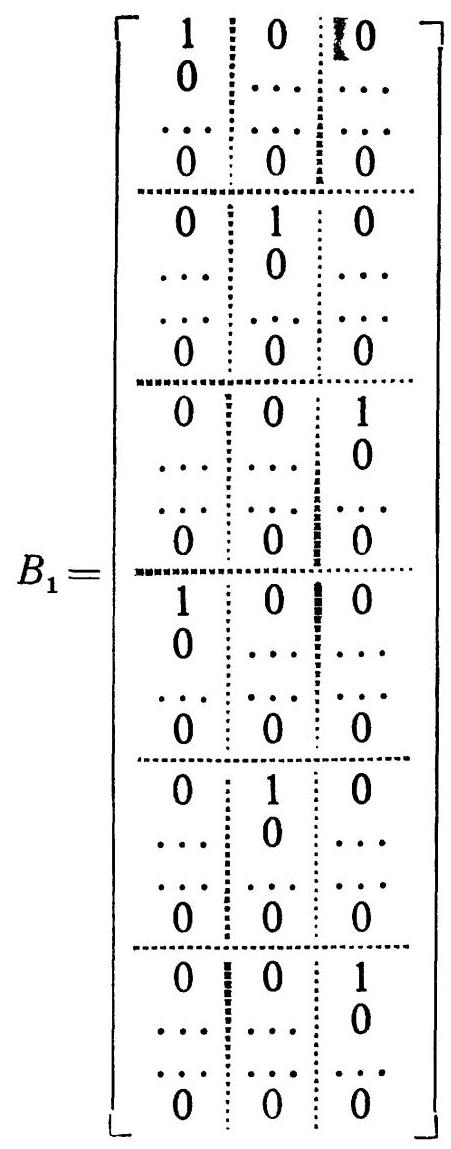
\includegraphics[max width=0.4\textwidth]{images/bo_d547k8bef24c73bgfcg0_120_580_243_451_1149_0.jpg}
\end{center}
\hspace*{3em} 

Так, 4ТО

\[
H{e}^{At}C{B}_{1} = \left\lbrack  \begin{array}{lll} {l}_{11} & {l}_{12} & {l}_{13} \\  {l}_{21} & {l}_{22} & {l}_{23} \end{array}\right\rbrack  ,
\]

что и требовалось доказать. Теорема доказана.

Рассмотрим автономную линейную наблюдаемую систему в R":

(2)
\[
\dot{x} = {Ax} + {Bu},\;\omega  = {Hx}.
\]

Постоянное линейное невырожденное преобразование в \({R}^{n}\)

\[
\bar{x} = {Px}
\]

позволяет преобразовать систему виду:

 \circled{2} 
\[
\dot{\bar{x}} = \bar{A}\bar{x} + \bar{B}u,\;\omega  = \bar{H}\bar{x},
\]

где А= \({PA}{P}^{-1},\bar{B} = {PB}\) ,и \(\bar{H} = H{P}^{-1}\) . Cuctemily \(\mathcal{L}\) и Z являются линейно эквивалентными относительно линейного преобразования \(\bar{x} = {Px}\) ; линейно эквивалентные наблюдаемые системы имеют одни и те же характерные свойства. Например, весовые матрицы таких систем совпадают, поскольку они не зависят от координат \(x\) B \({R}^{n}\) , T. e.

\[
W\left( t\right)  = H{e}^{tA}B = H{P}^{-1}{e}^{{tPA}{P}^{-1}}{PB} = \bar{H}{e}^{t\bar{A}}\bar{B},\;t \geq  0.
\]

Из теоремы 10 следует, что любая линейная автономная система, наблюдаемая в R",

(L)
\[
\dot{x} = {Ax} + {Bu},\;\omega  = {Hx},
\]

линейно эквивалентна наблюдаемой системе канонического вид

\[
\dot{{x}_{1}} = {\bar{A}}_{11}\overline{{x}_{1}} + {\bar{A}}_{12}\overline{{x}_{2}} + {\bar{B}}_{1}u,
\]

\[
{\bar{x}}_{3} = {\bar{A}}_{22}{\bar{x}}_{2}
\]

и

\[
\omega  = {\bar{H}}_{1}{\bar{x}}_{1} + {\bar{H}}_{2}{\bar{x}}_{2}.
\]

Здесь \(\bar{x} = \left( \frac{{\bar{x}}_{1}}{{\bar{x}}_{2}}\right)  -\) координаты в \({R}^{n}\) , a уравнение \({x}_{2} = 0\) определяет обладающую свойством управляемости часть системы 𝒳, причем система 𝒳 обладает свойством управляемости тогда и только тогда, когда совокупность координат х. пуста, т. е. й. преределяет все пространство \({R}^{n}\) . Наблюдаемая система У называется пол- ностью неуправляемой (или свободной), если пусто множество координат \({x}_{1}\) , т. е. В =0. Каждую систему £ можно разложить на систему, определенную на \({\bar{x}}_{2} = 0 : {\dot{\bar{x}}}_{1} = {\bar{A}}_{11}{\bar{x}}_{1} + {\bar{B}}_{1}u\) (эта система обладает свойством управляемости), и на систему х, не и хорцо про екцию системы 8 на подпространство \({x}_{1} = 0\) ,которая полностью неуправляема. Таким образом, вполне управляемую наблюдаемую систему можно определить, как систему, не содержащую пол- ностью неуправляемой части.

Аналогично можно назвать полностью ненаблюдаемой систему вида

\[
\dot{x} = {Ax} + {Bu},\;\omega  = 0,
\]

т. e. систему, у которой H=0. Наблюдаемую систему, не имею- щую такой полностью ненаблюдаемой части, естественно назвать вполне наблюдаемой.

Определение. Автономная линейная наблюдаемая система B \({R}^{n}\)

(L)
\[
\dot{x} = {Ax} + {Bu},\;\omega  = {Hx}
\]

называется влолие иаблюбаной, если она не является линейно эквивалентной никакой системе вида

bucket

\[
{\dot{\bar{x}}}_{1} = {\bar{A}}_{11}{\bar{x}}_{1} + {\bar{A}}_{12}{\bar{x}}_{2} + {\bar{B}}_{1}u
\]

\[
{\dot{\overline{x}}}_{2} = {\bar{A}}_{22}{\bar{x}}_{2} + {\bar{B}}_{2}u
\]

\({\mathbf{u}}_{j}\)

\[
\omega  = \overline{{H}_{2}{x}_{2}},
\]

где \(\bar{x} = \left( \frac{{\bar{x}}_{1}}{{\bar{x}}_{2}}\right)\) и множество \({\bar{x}}_{1}\) непусто.

Sametim. yro. ec.ili. Currema \& Jonovskaer Такое Idencrablehye C. Henvcrox royndox kooniuhaz x. to cyxichie cuctomly, ha подпространство \({x}_{2} = 0\) (например,для \(u = 0\) ),имеет вид

\[
{\dot{x}}_{1} = {\bar{A}}_{11}{\bar{x}}_{1},\;\omega  = 0.
\]

Последняя система является полностью ненаблюдаемой. Ниже мы определим разложение произвольной линейной автономной системы на вполне наблюдаемую и полностью ненаблюдаемую часть, и покажем, что система 8 будет вполне наблюдаемой лишь в том случае, если свободная система с и е≡0 не имеет нетривиального решения \(x\left( t\right)\) ,для которого бы ω (t) \(\equiv  0\) .

Теорема 13. Автономная линейная наблюдаемая система в R"

(L)
\[
\dot{x} = {Ax} + {Bu},\;\omega  = {Hx}
\]

является вполне наблюдаемой в том и только том случае, если двойственная динамическая система

\[
\left( {\mathcal{L}}^{\prime }\right)
\]

\[
\dot{x} = {A}^{\prime }x + {H}^{\prime }u,\;\omega  = {B}^{\prime }x
\]

будет вполне управляемой. А это будет тогда и только тогда, когда

\[
\operatorname{rank}\left\lbrack  {{H}^{\prime },{A}^{\prime }{H}^{\prime },{A}^{\prime 2}{H}^{\prime },\ldots ,{A}^{\prime n - 1}{H}^{\prime }}\right\rbrack   = n.
\]

Доказательство. Система Q не является вполне наблю- даемой лишь в том случае, если существует такое преобразование координат \(\bar{x} = \left\lbrack  \begin{array}{l} {\bar{x}}_{1} \\  {\bar{x}}_{2} \end{array}\right\rbrack   = {Px}\) (с непустой совокупностью коорди- нат \({\bar{x}}_{1}\) ),что

\[
\bar{A} = {PA}{P}^{-1} = \left\lbrack  \begin{array}{ll} {\bar{A}}_{11} & {\bar{A}}_{12} \\  0 & {\bar{A}}_{22} \end{array}\right\rbrack  ,
\]

\[
\bar{B} = {PB} = \left\lbrack  \begin{array}{l} {\bar{B}}_{1} \\  {\bar{B}}_{2} \end{array}\right\rbrack  \text{ и }\bar{H} = H{P}^{-1} = \left( {0,{\bar{H}}_{2}}\right) .
\]

Но тогда под действием преобразования \(\widetilde{x} = \left\lbrack  \begin{array}{l} {\widetilde{x}}_{1} \\  {\widetilde{x}}_{2} \end{array}\right\rbrack   = {\left( {P}^{-1}\right) }^{\prime }x\) коэффициенты системы \({\mathcal{L}}^{\prime }\) примут вид

\[
{P}^{-{1}^{\prime }}{A}^{\prime }{P}^{\prime } = \left\lbrack  \begin{array}{ll} {\bar{A}}_{11}^{\prime } & 0 \\  {\bar{A}}_{12}^{\prime } & {\bar{A}}_{22}^{\prime } \end{array}\right\rbrack  ,
\]

\[
{P}^{-1}{}^{\prime }{H}^{\prime } = \left\lbrack  \begin{array}{l} 0 \\  {\bar{H}}_{2}^{\prime } \end{array}\right\rbrack  \text{ и }{B}^{\prime }{P}^{\prime } = \left\lbrack  {{\bar{B}}_{1}^{\prime },{\bar{B}}_{2}^{\prime }}\right\rbrack  ,
\]

rak yto curroma. \%’ 6Vier hevupabile. Ahajorytho moxkho dokajath. yto.edu chetema \({\mathcal{L}}^{\prime }\) hevi.dajaga.go.uk.to.dkv.co.kr Heushorization

Mizk current y promise habionasma r tom y toutro tou случае, если система ./ вполне управляема, т. е. если

\[
\operatorname{rank}\left\lbrack  {{H}^{\prime },{A}^{\prime }{H}^{\prime },{A}^{\prime 2}{H}^{\prime },\ldots ,{A}^{\prime n - 1}{H}^{\prime }}\right\rbrack   = n.
\]

Теорема доказана.

Заметим, что система 8′ является двойственной к системе Z и поэтому она вполне управляема тогда и только тогда, когда система 8 вполне наблюдаема. Отмеченное здесь свойство двой- ственности показывает, что теоремам об управляемости должны соответствовать двойственные к ним теоремы о наблюдаемости (см. ниже упражнение 4). Например, следующая лемма опреде- ляет ненаблюдаемую часть свободной наблюдаемой системы.

Ле мма 1. Рассмотрим линейную автономную систему

\[
\left( \mathcal{L}\right)
\]

\[
\dot{x} = {Ax},\;\omega  = {Hx},
\]

которая является полностью неуправляемой в R". Тогда сущест- вует единственное линейное подпространство И, некоторой макси- мальной размерности l (0 ≤ l ≤ n) такое, что

(a) подпространство U инвариантно;

(b) сужение системы I на подпространство U есть полностью ненаблюдаемая система.

Система Ф будет вполне наблюдаемой тогда и только тогда, когда \(\mathcal{U} = 0\) . В соответствующей системе координат \(\bar{x} = \left( \begin{array}{l} {\bar{x}}_{1} \\  {\bar{x}}_{2} \end{array}\right)\) , в которой подпространство U задается уравнением х, =0, данная система описывается так:

\[
{\dot{\bar{x}}}_{1} = {\bar{A}}_{11}{\bar{x}}_{1} + {\bar{A}}_{12}{\bar{x}}_{2},{\bar{x}}_{2} = {\bar{A}}_{22}{\bar{x}}_{2}
\]

\(u\)

\[
\omega  = \overline{{H}_{2}}\overline{{x}_{2}}.
\]

На nodnpocmpaнстве x \({\bar{x}}_{1} = 0\) , \(\kappa\) omopoe будет нулевым при l = n, система

\[
{\dot{\bar{x}}}_{2} = {\bar{A}}_{22}{\bar{x}}_{2},\;\omega  = {H}_{2}{\bar{x}}_{2}
\]

6VDem Frank HabriodgeMOV.

dokasate. Femy 9L y N M - ma urranuatury nor Procrdahetra, На kotophix currena, e’illojitochio hemagnoraema, to \(\omega  = {ax}\) over toxing the market is human by no ha nonlinearity. 91 - 91 Creporatellity, 41 Ly, takke oviet ultraduanthim non-programctron, currently, \({\mathcal{G}}^{ - }\) ha koronom, Oha nonhorho Hehaómo- даема. Определим линейное пространство \(\mathcal{U}\) как сумму всех инва- риантных линейных подпространств, на которых система ℐ пол- ностыо ненаблюдаема. Такое пространство И по построению будет инварнантным подпространством, на котором \(\mathcal{L}\) полностыо нена- блюдаема, причем любое другое подпространство с теми же свойствами будет иметь размерность, менышую, чем Ч.

B соответствующих координатах \(\bar{x} = \left\lbrack  \begin{array}{l} {\bar{x}}_{1} \\  {\bar{x}}_{2} \end{array}\right\rbrack\) , B которых под- пространство И задается уравнением ха, ее, о, система примет вид, указанный в формулировке леммы. Если l < n, то совокупность координат \({\bar{x}}_{2}\) непуста, \(u\) спроектированная на это подпространство система

\[
{\dot{\bar{x}}}_{2} = {\bar{A}}_{22}{\bar{x}}_{2},\;\omega  = {\bar{H}}_{2}{\bar{x}}_{2}
\]

будет вполне наблюдаемой; действительно, в противном случае пространство U допускало бы дальнейшее разложение \({\bar{x}}_{2} = \left\lbrack  \begin{array}{l} {\bar{x}}_{3} \\  {\bar{x}}_{4} \end{array}\right\rbrack\) , что противоречило бы его свойству максимальности.

Итак, размерность l будет равняться n лишь в случае, когда \(H = 0\) , т. е. когда система gp полностью ненаблюдаема, и l = 0 лишь в случае, когда совокупность координат \({\bar{x}}_{1}\) пуста, т. е. система £ является вполне наблюдаемой.

Таким образом, из равенства Ие О (следует полная наблю- даемость системы У. Обратно, если система 8 вполне наблюдаема, то в разложении, указанном в формулировке леммы, совокупность координат \({x}_{1}\) -пуста, \(\tau\) . e. \(\mathcal{U} = 0\) . Лемма доказана.

Ниже мы дадим удобную каноническую форму для линейных вполне наблюдаемых и вполне управляемых систем. Она потре- буется нам для построения примеров таких систем. Мы будем рассматривать здесь лишь случай m=1, т. е. системы со скаляр- ными управлениями и (t), так как для этого случая теорема 7 дает основную каноническую форму линейной вполне управляемой GUCTEMEN

Ле мма 2. Рассмотрим наблюдаемую автономную систему в R":

(Y)
\[
\dot{x} = {Ax} + {bu},\;u \in  {R}^{1},\;\omega  = {Hx}.
\]

Преблогожсим,чпо 오 впогие управгяемая сисгема и что

\[
A = \left[ \begin{array}{ccccccc} 0 & 1 & 0 & 0 & \ldots & 0 & 0 \\  0 & 0 & 1 & 0 & \ldots & 0 & 0 \\  \vdots & & & & & & \\  0 & 0 & 0 & 0 & \ldots & 0 & 1 \\  {a}_{n} &  - {a}_{n - 1} &  - {a}_{n - 2} & \ldots & \ldots &  - {a}_{2} &  - {a}_{1} \end{array} \right]  ,\;b = \left[ \begin{array}{c} 0 \\  0 \\  \vdots \\  0 \\  1 \end{array} \right]  ,
\]

\[
H = \left[ \begin{array}{cccc} {b}_{1n} & {b}_{1,n - 1} & \ldots & {b}_{11} \\  {b}_{2n} & {b}_{2,n - 1} & \ldots & {b}_{21} \\  . & . & . & . \\  {b}_{rn} & {b}_{r,n - 1} & \ldots & {b}_{r1} \end{array} \right]  .
\]

Тогда система Ц будет вполне наблюдаемой в том и только том случае, если многочлены

\(u\)

\[
D\left( p\right)  = {p}^{n} + {a}_{1}{p}^{n - 1} + \ldots  + {a}_{n}
\]

\[
{N}_{1}\left( p\right)  = {b}_{11}{p}^{n - 1} + {b}_{12}{p}^{n - 2} + \ldots  + {b}_{1n},
\]

\[
{N}_{r}\left( p\right)  = {b}_{r1}{p}^{n - 1} + {b}_{r2}{p}^{n - 2} + \ldots  + {b}_{rn}
\]

не имеют общих корней.

Доказательство. В силу теоремы двойственности система Х будет вполне наблюдаемой тогда и только тогда, когда система

\[
\dot{x} = {Fx} + {Gu}
\]

будет вполне управляемой.Здесь

\[
F = \left[ \begin{array}{ccccc} 0 & 0 & \ldots & 0 &  - {a}_{n} \\  1 & 0 & \ldots & 0 &  - {a}_{n - 1} \\  0 & 1 & \ldots & 0 & \\  0 & 0 & \ldots & 0 & \\  \vdots & & & \vdots & \\  0 & 0 & \ldots & 1 &  - {a}_{n} \end{array} \right]   = {A}^{\prime },
\]

\[
G = \left[ \begin{array}{cccc} {b}_{1n} & {b}_{2n} & \ldots & {b}_{rn} \\  {b}_{1,n - 1} & {b}_{2,n - 1} & \ldots & {b}_{r,n - 1} \\  \vdots & & & \\  {b}_{11} & {b}_{21} & \ldots & {b}_{r1} \end{array} \right]   = I{I}^{\prime }.
\]

Таким образом, система 8 вполне наблюдаема тогда и только тогда,Екогда

\[
\operatorname{rank}\left\lbrack  {G,{FG},{F}^{2}G,\ldots ,{F}^{n - 1}G}\right\rbrack   = n.
\]

Введем обозначение

\[
\Delta \left\lbrack  {P,Q}\right\rbrack   = \left\lbrack  {Q,{PQ},{P}^{2}Q,\ldots ,{P}^{n - 1}Q}\right\rbrack  ,
\]

где \(P - \left( {n \times  m}\right)\) -матрица, a \(Q - n\) -вектор-столбец. Тогда Δ \(\left\lbrack  {P,Q}\right\rbrack\) есть матричнозначная функция двух матричных аргументов P и Q, линейная по Q. Вычислим значение этой функции при Р=F и \(Q = {\beta }_{j}\) ,где \({\beta }_{j}\) — столбец матрицы G.

Рассмотрим сначала последовательность \({e}_{1},{e}_{2},\ldots ,{e}_{n}\) векто- ров-столбцов единичной матрицы I. Заметим, что \({e}_{i + 1} = F{e}_{i}\) для \(1 \leq  i \leq  n - 1\) . Acho,что

\[
\Delta \left\lbrack  {F,{e}_{1}}\right\rbrack   = \left\lbrack  {{e}_{1}{e}_{2}\ldots {e}_{n}}\right\rbrack   = I
\]

H

\[
\Delta \left\lbrack  {F,{e}_{i}}\right\rbrack   = \Delta \left\lbrack  {F,{F}^{i - 1}{e}_{1}}\right\rbrack   = {F}^{i - 1}\Delta \left\lbrack  {F,{e}_{1}}\right\rbrack   = {F}^{i - 1}
\]

аля \(1 \leq  i \leq  n\) . 3апншем j-й столбец матрицы G в виде

NMeeM

\[
{\beta }_{j} = {b}_{jn}{e}_{1} + {b}_{{jn} - 1}{e}_{2} + \ldots  + {b}_{j1}{e}_{n}.
\]

\[
\Delta \left\lbrack  {F,{\beta }_{j}}\right\rbrack   = {b}_{jn}I + {b}_{{jn} - 1}F + \ldots  + {b}_{j1}{F}^{n - 1} = {N}_{j}\left( F\right) .
\]

Таким образом, ранг матрицы [G, F G, ..., Fr-1G] равен рангу ма- трицы \(\left\lbrack  {{N}_{1}\left( F\right) ,{N}_{2}\left( F\right) ,\ldots ,{N}_{r}\left( F\right) }\right\rbrack\) ,поскольку эти две матрицы отличаются друг от друга лишь расположением столбцов.

При вычислении ранга матрицы \(\left\lbrack  {{N}_{1}\left( F\right) ,\ldots ,{N}_{r}\left( F\right) }\right\rbrack\) для задан- ных многочленов \({N}_{1},\ldots ,{N}_{r}\) удобно воспользоваться той систе- мой (возможно, комплексных) координат, в которой матрица F имеет треугольный вид, например,

\[
\left[ \begin{array}{ccccc} {\lambda }_{1} & 0 & 0 & \ldots & 0 \\   * & {\lambda }_{2} & 0 & \ldots & 0 \\   \cdot  &  \cdot  &  \cdot  & & \\   \cdot  &  \cdot  &  \cdot  & & \\   \cdot  &  \cdot  &  \cdot  &  \cdot  & {\lambda }_{n} \end{array} \right]
\]

Здесь \({\lambda }_{1},{\lambda }_{2},\ldots ,{\lambda }_{n}\) —собственные значения матрицы \(A\) ,и сле- довательно, корни многочлена — D (р). Тогда ранг матрицы \(\left\lbrack  {{N}_{1}\left( F\right) ,\ldots ,{N}_{r}\left( F\right) }\right\rbrack\) совпадает с рангом следующей матрицы:

\[
M = \left[ \begin{array}{ccc} {N}_{1}\left( {\lambda }_{1}\right) & & 0 \\   &  \ddots  & \\   * & & {N}_{1}\left( {\lambda }_{n}\right) \end{array} \right]  \left[ \begin{array}{ccc} {N}_{2}\left( {\lambda }_{1}\right) & & 0 \\   &  \ddots  & \\   * & & {N}_{2}\left( {\lambda }_{n}\right) \end{array} \right]  \cdots \left[ \begin{array}{ccc} {N}_{r}\left( {\lambda }_{1}\right) & & 0 \\   &  \ddots  & \\   * & & {N}_{r}\left( {\lambda }_{n}\right) \end{array} \right]  .
\]

Предположим, что среди корней \({\lambda }_{1},{\lambda }_{2},\ldots ,{\lambda }_{n}\) многочлена \(D\left( p\right)\) имеется корень, скажем, \({\lambda }_{1}\) , являющийся также корнем каждого из многочленов \({N}_{1}\left( p\right) ,{N}_{2}\left( p\right) ,\ldots ,{N}_{r}\left( p\right)\) . Тогда первая строка marginal by oyaes coctogity has human, a shaght, pani se memb-we n. T. e. current C. Bangerca Hemoß Takaho Odoa3OM ECJU CHICTEMA Y BIOJIE HAGIOJIEMA ТО MHOТОYJEHD D. N., Algorithment forms konney.

Objatho neighbourway pro 'wworou.letty. \(D,N,N,N,N,N\) HE NMEТОOLINX KOPHER. IOTДL один из многочленов \({N}_{j}\) ,например, \({N}_{j1}\) . Выберем тот столбец матрицы [M], который содержит элемент \({N}_{{j}_{1}}\left( {\lambda }_{1}\right)  \neq  0\) на главной диагонали соответствующей \(\left( {n \times  n}\right)\) -субматрицы матрицы [M]. Выберем такие столбцы матрицы [M] для каждого значения \({\lambda }_{1}\) , \({\lambda }_{2},\ldots ,{\lambda }_{n}\) ; ясно, что полученные таким образом n-столбцов будут линейно независимы. Значит, матрица [M] имеет ранг n, и си- стема gp вполне наблюдаема. Лемма доказана.

Следующая теорема, являющаяся основным результатом на- стоящего раздела, объединяет два подхода в линейной теории управления: теорию передаточных функций и описание наблюдае- мых систем с помощью дифференциальных уравнений.

Teopeм a 14. Пусть Z(p)—ненулевая (r×m)-матрица, эле- менты которой есть правильные дробно-рациональные функции (степени числителей меньше степеней знаменателей). Тогда суще- ствует действительная автономная линейная система

(Y)
\[
\dot{x} = {Ax} + {Bu},\;\omega  = {Hx}
\]

вполне управляемая и вполне наблюдаемая, для которой Z (р) слу- жит передаточной матричной функцией. При т=1 такая система единственна с точностью до линейной эквивалентности.

Доказательство. На основании теоремы 12 матрицу Z(p) можно представить в качестве передаточной функции некоторой автономной линейной наблюдаемой системы в RN:

(3)
\[
\dot{x} = {Ax} + {Bu},\;\omega  = {Hx}.
\]

Если выбрать в \({R}^{N}\) систему координат \(x = \left\lbrack  \begin{array}{l} {x}_{a} \\  {x}_{b} \end{array}\right\rbrack\) , oбладающую свойством, сформулированным в следствии из теоремы 10, то вполне управляемая часть системы Ф получится сужёнием ее на подпространство \({x}_{b} = 0\) , a вся наблюдаемая система запишется в виде

\[
{\dot{x}}_{a} = {A}_{aa}{x}_{a} + {A}_{ab}{x}_{b} + {B}_{a}u,
\]

и

\[
{x}_{b} = {A}_{bb}{x}_{b}
\]

\[
\omega  = {H}_{a}{x}_{a} + {H}_{b}{x}_{b}.
\]

Заметим, что совокупность координат ха непуста, так как иначе матрица \(B\) равнялась бы нулю, т. е. система Ф была бы пол- ностью неуправляемой, а ее передаточная функция — нулевой. Далее, система 𝒳, рассматриваемая лишь на подпространстве \({x}_{b} = 0\) , oбладает свойством управляемости и записывается в виде

\[
\left( {\mathcal{L}}_{a}\right)
\]

\[
{\dot{x}}_{a} = {A}_{aa}{x}_{a} + {B}_{a}u\;\text{ и }\;\omega  = {H}_{a}{x}_{a}.
\]

Система \({\mathcal{L}}_{a}\) имеет тужевесовую матрнцу,чтоистема \(\widetilde{\mathcal{L}}\) ,ибо

\[
H{e}^{tA}B = \left( {{H}_{a},{H}_{b}}\right) \left[ \begin{array}{cc} {e}^{t{A}_{aa}} &  * \\  0 & {e}^{t{A}_{bb}} \end{array} \right]  \left[ \begin{array}{c} {B}_{a} \\  0 \end{array} \right]   = {H}_{a}{e}^{t{A}_{aa}}{B}_{a}.
\]

Тем самым передаточной функцией системы У. будет матрица \(Z\left( p\right)\) .

Определим теперь систему координат \({x}_{a} = \left\lbrack  \begin{array}{l} {x}_{1} \\  {x}_{2} \end{array}\right\rbrack\) ,как указано в лемме 1, с тем, чтобы выделить вполне наблюдаемую часть си- стемы \({\mathcal{L}}_{a}\) . Тогда система \({\mathcal{L}}_{a}\) запишется в виде

\[
\left( {\mathcal{L}}_{a}\right)
\]

\[
{\dot{x}}_{1} = {A}_{11}{x}_{1} + {A}_{12}{x}_{2} + {B}_{1}u,{\dot{x}}_{2} = {A}_{22}{x}_{2} + {B}_{2}u
\]

и

\[
\omega  = {H}_{2}{x}_{2}.
\]

Здесь множество координат \({x}_{2}\) непусто, ибо в противном случае \({H}_{a} = 0\) , cutc푸Ma \({\mathcal{L}}_{a}\) полностью ненаблюдаема и, следовательно, имеет нулевую передаточную матричную функцию. Далее проекция системы 8. на подпространство \({x}_{1} = 0\) вполне наблюдаема (в лемме 1 рассматривался случай, когда вае 10,000 кспн июня и же м наблюдаемости системы не зависит от Ва)

(B)
\[
{\dot{x}}_{2} = {A}_{22}{x}_{2} + {B}_{2}u
\]

\[
\omega  = {H}_{2}{x}_{2}
\]

Покажем теперь, что система \(\mathcal{L}\) обладает свойством управляемости. Система \({\mathcal{L}}_{a}\) порядка \({n}_{a}\) вполне управляема и,следовательно,

\[
\operatorname{rank}\left[ \begin{array}{ccccc} * &  * &  * & \ldots &  * \\  {B}_{2}, & {A}_{22}{B}_{2}, & {A}_{22}^{2}{B}_{2}, & \ldots , & {A}_{22}^{{n}_{a} - 1}{B}_{22} \end{array} \right]   = {n}_{a}.
\]

Такнм образом, строкн матрицы

\[
\left\lbrack  {{B}_{2}{A}_{22}{B}_{2}{A}_{22}^{2}{B}_{2}\ldots {A}_{22}^{{n}_{a} - 1}{B}_{2}}\right\rbrack
\]

линейно независимы. Из теоремы Гамильтона—Кэли следует, что

\[
\operatorname{rank}\left\lbrack  {{B}_{2},{A}_{22}{B}_{2},{A}_{22}^{2}{B}_{2},\ldots ,{A}_{22}^{n - 1}{B}_{2}}\right\rbrack   = n,
\]

где л-порядок системы 𝒳. Поэтому система 𝒳 вполне управ- ляема и вполне наблюдаема. Весовая матричная функция систе- мы gp точности совпадает с весовой функцией системы \({\mathcal{L}}_{a}\) ,

так как

\[
{H}_{a}{e}^{t{A}_{aa}}{B}_{a} = \left( {0,{H}_{2}}\right) \left[ \begin{array}{cc} {e}^{t{A}_{11}} &  * \\  0 & {e}^{t{A}_{22}} \end{array} \right]  \left\lbrack  \begin{array}{l} {B}_{1} \\  {B}_{2} \end{array}\right\rbrack   = {H}_{2}{e}^{t{A}_{22}}{B}_{2}.
\]

Таким образом, система 8 имеет требуемую передаточную функ- цию \(Z\left( p\right)\) .

Наконец, покажем, что, с точностью до линейной эквивалент- ности, система 8 единственна в R". Доказательство проведем для случая \(m = 1\) . В этом случае система 8 может быть записана в удобной эквивалентной форме:

и

(
\[
{\mathcal{L}}^{\prime }
\]
 )
\[
\dot{x} = \left[ \begin{array}{ccccccc} 0 & 1 & 0 & 0 & \ldots & 0 & 0 \\  0 & 0 & 1 & 0 & \ldots & 0 & 0 \\  \vdots & & & & & & \\  0 & 0 & 0 & 0 & \ldots & 0 & 1 \\   - {a}_{n}^{\prime } &  - {a}_{n - 1}^{\prime } & & & \ldots &  - {a}_{2}^{\prime } &  - {a}_{1}^{\prime } \end{array} \right]  x + \left[ \begin{array}{c} 0 \\  0 \\  \vdots \\  0 \\  1 \end{array} \right]  u
\]

\[
\omega  = \left[ \begin{array}{cccc} {b}_{1n}^{\prime } & {b}_{1,n - 1}^{\prime } & \ldots & {b}_{11}^{\prime } \\  {b}_{2n}^{\prime } & {b}_{2,n - 1}^{\prime } & \ldots & {b}_{21}^{\prime } \\  \ldots & \ldots & \ldots & \ldots \\  {b}_{rn}^{\prime } & {b}_{r,n - 1}^{\prime } & \ldots & {b}_{r1}^{\prime } \end{array} \right]  x.
\]

Матричная передаточная функция системы у

\[
Z\left( p\right)  = \frac{1}{{D}^{\prime }\left( p\right) }\left[ \begin{array}{c} {N}_{1}^{\prime }\left( p\right) \\   \cdot  \\   \cdot  \\   \cdot  \\  {N}_{r}^{\prime }\left( p\right) \end{array} \right]  ,
\]

где

\[
{D}^{\prime }\left( p\right)  = {p}^{n} + {a}_{1}^{\prime }{p}^{n - 1} + \ldots  + {a}_{n}^{\prime },
\]

\[
{N}_{1}^{\prime }\left( p\right)  = {b}_{11}^{\prime }{p}^{n - 1} + \ldots  + {b}_{1n}^{\prime }
\]

\[
{N}_{r}^{\prime }\left( p\right)  = {b}_{r1}^{\prime }{p}^{n - 1} + \ldots  + {b}_{rn}^{\prime }.
\]

Поскольку система 8/ вполне наблюдаема, то многочлены \({D}^{\prime },{N}_{1}^{\prime },\ldots ,{N}_{r}^{\prime }\) не имеют общих корней (обратите внимание на то, что знак (′) не означает здесь дифференцирования).

Мы докажем, что матричная передаточная функция

\[
Z\left( p\right)  = \frac{1}{D\left( p\right) }\left[ \begin{array}{c} {N}_{1}\left( p\right) \\  \vdots \\  {N}_{r}\left( p\right) \end{array} \right]
\]

определяет соответствующую вполне управляемую и вполне на- блюдаемую систему единственным образом. При этом многочлены, входящие в передаточную функцию, взаимно просты и имеют вид

\[
D\left( p\right)  = {p}^{n} + {a}_{1}{p}^{n - 1} + \ldots  + {a}_{n},
\]

\[
{N}_{1}\left( p\right)  = {b}_{11}{p}^{n - 1} + \ldots  + {b}_{1n},
\]

\[
{N}_{r}\left( p\right)  = {b}_{r1}{p}^{n - 1} + \ldots  + {b}_{rn}.
\]

Тем самым мы покажем, что две вполне управляемые и вполне наблюдаемые системы в \({R}^{n}\) , oбладающие одной и той же переда- точной функцией, будут эквивалентны. Имеем

\[
\frac{{N}_{j}\left( p\right) }{D\left( p\right) } = \frac{{N}_{j}^{\prime }\left( p\right) }{{D}^{\prime }\left( p\right) },\;j = 1,2,\ldots ,r
\]

II, 3HAUHT,

\[
D\left( p\right) {N}_{j}^{\prime }\left( p\right)  = {D}^{\prime }\left( p\right) {N}_{j}\left( p\right) .
\]

Если \(p = {\lambda }_{1}\) есть корень многочлена \(D\left( p\right)\) , то имеется многочлен \({N}_{{j}_{1}}\left( p\right)\) ,для которого \({\lambda }_{1}\) не будет корнем. Следовательно,число \({\lambda }_{1}\) должне быть корнем многочлена \({D}^{\prime }\left( p\right)\) . Отсюда следует, что мно- гочлены \(D\left( p\right)\) и \({D}^{\prime }\left( p\right)\) имеют одни и те же корни, а поскольку коэффициенты при их старших членах равны +1, то \(D\left( p\right)  \equiv  {D}^{\prime }\left( p\right)\) (степени многочленов равны по условию). Аналогично доказывает- CA, ЧТО

\[
{N}_{j}\left( p\right)  \equiv  {N}_{j}^{\prime }\left( p\right) \;\left( {1 \leq  j \leq  r}\right) .
\]

Поэтому размерности \(r\) и \(n\) системы \({\mathcal{L}}^{\prime }\) определяются разме- рами матрицы \(Z\left( p\right)\) и степенью общего знаменателя D (p) в матрице \(Z\left( p\right)\) однозначно. Также определены и сами коэффициенты вполне наблюдаемой системы \_ℓ'. Итак, \_ℓ' есть единственная канони- ческая форма вполне управляемой, вполне наблюдаемой автономной линейной системы с передаточной функцией \(Z\left( p\right)\) . Теорема доказана.

\(\Pi\) ример. Рассмотрим случай r=m=1 и построим вполне управляемую и вполне наблюдаемую систему, имеющую в ка- честве передаточной матрицы дробно-рациональную функцию

\[
\frac{N\left( p\right) }{D\left( p\right) } = \frac{{b}_{1}{p}^{n - 1} + {b}_{2}{p}^{n - 2} + \ldots  + {b}_{n}}{{p}^{n} + {a}_{1}{p}^{n - 1} + \ldots  + {a}_{n}},
\]

где многочлены \(N\left( p\right)\) и \(D\left( p\right)\) действительны и взаимно просты, причем N(p) = 0. Систему, соответствующую такой передаточной функции, можно описать дифференциальным уравнением, в пра- вую часть которого управление входит под знаком дифференци- ального оператора:

\[
{x}^{\left( n\right) } + {a}_{1}{x}^{\left( n - 1\right) } + \ldots  + {a}_{n}x = {b}_{1}{u}^{\left( n - 1\right) } + {b}_{2}{u}^{\left( n - 2\right) } + \ldots  + {b}_{n}u.
\]

Однако такое уравнение непосредственно не определяет наблюдае- мой системы, поскольку оно содержит производные от управляю- щей функции и (t). Здесь можно использовать разрывные релейные управления, однако при этом не обойтись без применения методов теории обобщенных функций. Но так как соответствующая теория нами не была предварительно развита, то мы обратимся к другому методу построения наблюдаемой системы, соответствующей данной передаточной функции.

Рассмотрим систему

\[
{x}^{\left( n\right) } + {a}_{1}{x}^{\left( n - 1\right) } + \ldots  + {a}_{n}x = u,\omega  = {b}_{1}{x}^{\left( n - 1\right) } + \ldots  + {b}_{n}x,
\]

T. E. IOЛОСИМ

\[
A = \left[ \begin{array}{ccccc} 0 & 1 & 0\;0\;\ldots & 0 & 0 \\  0 & 0 & 1\;0\;\ldots & 0 & 0 \\  \vdots & & & & \\  0 & 0 & 0\;0\;\ldots & 0 & 1 \\   - {a}_{n} &  - {a}_{n - 1} & & \ldots &  - {a}_{2} - {a}_{1} \end{array} \right]  ,\;B = \left[ \begin{array}{c} 0 \\  0 \\  \vdots \\  0 \\  1 \end{array} \right]
\]

H

\[
H = \left( {{b}_{n},{b}_{n - 1},\ldots ,{b}_{2},{b}_{1}}\right) .
\]

Такая система является вполне управляемой и вполне наблюдае- мой, а ее передаточной функцией будет \(N\left( p\right) /D\left( p\right)\) .

Напоминаем, что доказательство единственности системы, соот- ветствующей данной передаточной функции и обладающей свойст- вами управляемости и наблюдаемости, проведено нами лишь для случая \(m = 1\) и опущено для более сложного случая m>1. Отметим также, что теорию управляемости и наблюдаемости можно распространить и на неавтономные линейные системы (см. упраж- нения), однако в этом случае удобные критерии, сформулирован- ные в теоремах 5 и 13, будут непригодны.

Последней темой, обсуждаемой в этом разделе, будет задача следующего типа: найти такое управление, чтобы система из не- которого начального состояния х перешла за конечный промежуток времени в заданное непустое целевое множество G, и в дальнейшем оставалась в этом множестве. Наиболее интересным здесь будет случай, когда наблюдаемыми являются несколько компонентов вектора состояния — \({x}^{1},{x}^{2},\ldots ,{x}^{r}\) и их требуется привести к нулю и далее сохранять их нулевые значения. В этом случае целевое множество G будет линейным подпространством \({x}^{1} = 0,{x}^{2} = 0,\ldots \; \ldots ,{x}^{r} = 0\) npocтранства \({R}^{n}\) .

Определение. Рассмотрим линейную автономную систему B \({R}^{n}\) :

\[
\left( \mathcal{L}\right)
\]

\[
\dot{x} = {Ax} + {Bu}
\]

с компактным ограничивающим множеством \(\Omega  \subset  {R}^{m}\) и целевым множеством \(G \subset  {R}^{n}\) . Назовем ядром множества G и обозначим через core (G) совокупность всех точек \({x}_{1} \in  G\) ,для которых суще- ствует допустимое управление и (t) с Ω на 0 ≤ s < c < ∞, такое, что под его воздействием система из точки \({x}_{1}\) перемещается далее по траектории \({x}_{1}\left( t\right)  \subset  G\) на \(0 \leq  t < \infty\) .

Из этого определения следует, что если требуется перевести систему в желаемую область G и затем удерживать ее в этой области, то можно просто сказать, что требуется перевести систему в область, являющуюся ядром области G. Таким образом, задача приведения системы из точки х, в область G с дальнейшим удер- живанием траектории системы в G может быть сведена к задаче приведения системы в ядро области G без какого-либо рассмотре- ния дальнейшего поведения системы.

Teopeм a 15. Рассмотрим автономную линейную управляемую систему в R":

(Y)
\[
\dot{x} = {Ax} + {Bu},
\]

с компактным выпуклым ограничивающим множеством Ω⊂R™ и замкнутым выпуклым целевым множеством G. Тогда соге (G) есть замкнутое выпуклое подмножество множества G. Более того,

\[
\text{ core }\left( {\operatorname{core}\left( G\right) }\right)  = \operatorname{core}\left( G\right) \text{ . }
\]

Доказательство. Пусть х, и и хд —начальные состояния системы, из которых она переводится в область \(G\) с помощью управлений \({u}_{1}\left( t\right)\) и \({u}_{2}\left( t\right)  \in  \Omega\) на \(0 \leq  t < \infty\) coorbeтственно. Тогда

\[
{x}_{i}\left( t\right)  = {e}^{At}{x}_{l} + {e}^{At}{\int }_{0}^{t}{e}^{-{As}}B{u}_{i}\left( s\right) {ds},\;i = 1,2.
\]

Если \(0 \leq  \lambda  \leq  1\) , ТО

\[
\lambda {x}_{1}\left( t\right)  + \left( {1 - \lambda }\right) {x}_{2}\left( t\right)  = {e}^{At}\left( {\lambda {x}_{1} + \left( {1 - \lambda }\right) {x}_{2}}\right)  +
\]

\[
+ {e}^{At}{\int }_{0}^{t}{e}^{-{As}}B\left( {\lambda {u}_{1}\left( s\right)  + \left( {1 - \lambda }\right) {u}_{2}\left( s\right) }\right) {ds},
\]

и поэтому управление \(\left\lbrack  {\lambda {u}_{1}\left( t\right)  + \left( {1 - \lambda }\right) {u}_{2}\left( t\right) }\right\rbrack   \subset  \Omega\) на \(0 \leq  t \leq  \infty\) переводит систему из точки [λx+(1-λ)x, в область G. Таким образом, соге (G) есть выпуклое множество.

Пусть \({x}_{1},{x}_{2},\ldots  -\) последовательность точек из ядра множе- ства G и \(\mathop{\lim }\limits_{{k \rightarrow  \infty }}{x}_{k} = \bar{x} \in  G\) . Пусть \({u}_{1}\left( t\right) ,{u}_{2}\left( t\right) ,\ldots\) -соответствующие им управления, удерживающие \({x}_{1},{x}_{2},\ldots\) в G. Выберем такую под- последовательность точек (мы будем обозначать ее снова х, х, х,.,. . .), чтобы \(\mathop{\lim }\limits_{{k \rightarrow  \infty }}{u}_{k}\left( t\right)  = \bar{u}\left( t\right)  \subset  \Omega\) в смысле слабой сходимости на любом конечном интервале 0≤た≤t,- Тогда решение, соответствующее предельному управлению, будет

\[
\bar{x}\left( t\right)  = {e}^{At}\bar{x} + {e}^{At}{\int }_{0}^{t}{e}^{-{As}}B\bar{u}\left( s\right) {ds}
\]

H

\[
\bar{x}\left( t\right)  = \mathop{\lim }\limits_{{k \rightarrow  \infty }}{x}_{k}\left( t\right)
\]

для любого фиксированного \(t \geq  0\) . Поскольку G-замкнутое мно- жество, то \(x\left( t\right)  \subset  G\) для всех \(t \geq  0\) . Поэтому хе с соге (G) и с соге (G) является замкнутым множеством.

Если точка \({x}_{0}\) принадлежит ядру \(G\) ,то некоторому управлению \(u\left( t\right)  \subset  \Omega\) на интервале 0 ≤ t < ∞ соответствует решение \({x}_{0}\left( t\right)  \subset  G\) . Но тогда для любого фиксированного \(t \geq  0{x}_{0}\left( t\right)\) служит началь- ной точкой некоторой траектории, целиком лежащей в G с управ- лением \(u\left( t\right)  \subset  \Omega\) . Cледовательно, \({x}_{0}\left( t\right)  \in  \operatorname{core}\left( G\right)\) для любого \(t \geq  0\) . Таким образом, \({x}_{0} \in  \operatorname{core}\left( {\operatorname{core}\left( G\right) }\right)\) и,значит,

\[
\text{ core }\left( {\operatorname{core}\left( G\right) }\right)  = \operatorname{core}\left( G\right) \text{ . }
\]

Теорема доказана.

Часто бывает затруднительно установить, компактно ли ядро G, даже если G является линейным подпространством пространства R* (см. пример в разделе 1.3). Однако в задачах на быстродействие наиболее отдаленные части области G обычно исключаются из рассмотрения. Поэтому задачи с компактным целевым множеством встречаются достаточно часто.

В случае, когда множество G является линейным подпростран- ством, соответствующую управляемую систему называют системой с регулированием по многим компонентам. Следующая теорема по- казывает, что такие задачи чаще всего можно свести к задачам с регулированием по одной компоненте,

Теорема 16. Рассмотрим автономную линейную управляемую систему в R":

(L)
\[
\dot{x} = {Ax} + {bu}
\]

с компактным ограничивающим интервалом Ω ⊂ R1, содержащим точку и =0. Предположим, что система Q обладает свойством управляемости, и возьмем некоторое подпространство π прост- ранства R". Тогда существует такая гиперплоскость π размер- ности n-1, что

\[
\operatorname{core}\left( \widehat{\pi }\right)  = \operatorname{core}\left( \pi \right) \text{ . }
\]

Доказательство. core(π) является замкнутым выпуклым подмножеством множества π, непустым, так как оно должно содержать точку х=0; следовательно, оно имеет непустую внут- ренность, порождающую некоторое линейное подпространство

\({\pi }_{1} \subset  \pi\) paзмерности \(\left( {n - r}\right)\) . core \(\left( {\pi }_{1}\right)\) должно совпадать с core \(\left( \pi \right)\) . Выберем координаты \(\bar{x} = \left\lbrack  \begin{array}{l} {\bar{x}}_{1} \\  {\bar{x}}_{2} \end{array}\right\rbrack\) в \({R}^{n}\) так,чтобы подпространство \({\pi }_{1}\) задавалось уравнениями \({\bar{x}}_{1} = \left[ \begin{array}{c} {\bar{x}}^{1} \\  \vdots \\  {\bar{x}}^{r} \end{array} \right]   = 0\) (если тд состоит из одной точки —начала координат, то совокупность координат х, пуста). Запишем систему 𝒳 в виде

\[
{\dot{\bar{x}}}_{1} = {\bar{A}}_{11}{\bar{x}}_{1} + {\bar{A}}_{12}{\bar{x}}_{2}{\bar{b}}_{1}u,\;{\dot{\bar{x}}}_{2} = {\bar{A}}_{21}{\bar{x}}_{1} + {\bar{A}}_{22}{\bar{x}}_{2} + {\bar{b}}_{2}u.
\]

Предположим,что \({\bar{b}}_{1} = 0\) . Тогда в тех точках core \(\left( {\pi }_{1}\right)\) ,где \({\bar{x}}_{1} = 0\) , имеем \(\dot{x} = 0\) и \({\bar{A}}_{12}{\bar{x}}_{2} = 0\) . Поскольку в подпространстве я имеются внутренние точки core \(\left( {\pi }_{1}\right)\) , to \({\bar{A}}_{12} = 0\) . Но это означает,что

\[
\dot{{x}_{1}} = {\bar{A}}_{11}{\bar{x}}_{1},
\]

что противоречит управляемости системы. Поэтому Б1, = 0.

Определим новые координаты в пространстве R" так, чтобы подпространство \({\pi }_{1}\) задавалось соотношением \({\bar{x}}_{1} = 0\) ,冊ичем

\[
{\bar{b}}_{1} = \left[ \begin{array}{c} 0 \\  0 \\  \vdots \\  1 \end{array} \right]
\]

и запншем

\[
{\bar{A}}_{12} = \left[ \begin{array}{ccc} {a}_{r + 1}^{1} & \ldots & {a}_{n}^{1} \\  \vdots & & \\  {a}_{r + 1}^{r} & \ldots & {a}_{n}^{r} \end{array} \right]  .
\]

Предположим, что k-я строка матрицы A12, 1 ≤k < r содержит ненулевые элементы. Тогда

\[
\dot{{\bar{x}}^{k}} = {a}_{r + 1}^{k}{\bar{x}}^{r + 1} + \ldots  + {a}_{n}^{k}\overline{{x}^{n}} = 0
\]

во всех точках core \(\left( {\pi }_{1}\right)\) . Но это означает, что core \(\left( {\pi }_{1}\right)\) содepжится в пересечении подпространств

\[
\overline{{x}^{1}} = \overline{{x}^{2}} = \ldots  = \overline{{x}^{r}} = 0\text{ и }{a}_{r + 1}^{k}\overline{{x}^{r + 1}} + \ldots  + {a}_{n}^{k}\overline{{x}^{n}} = 0,
\]

что противоречит предположению о том, что размерность core \(\left( {\pi }_{1}\right)\) равна (n-r). Таким образом,

\begin{center}
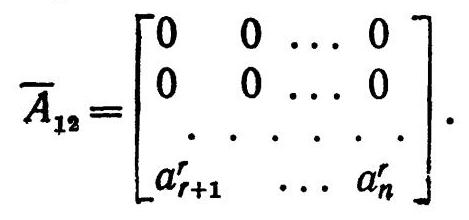
\includegraphics[max width=0.4\textwidth]{images/bo_d547k8bef24c73bgfcg0_134_580_1940_469_220_0.jpg}
\end{center}
\hspace*{3em} 

Для любых двух точек ( \(\overline{{x}_{1a}},0\) ) и \(\left( {\overline{{x}_{1b}},0}\right)\) в \({R}^{n}\) существует управ- ление \(u\left( t\right)  \subset  {R}^{1}\) , переводящее систему из первой точки во вторую вдоль траектории \(\bar{x}\left( t\right)\) . Но тогда управление

\[
\bar{u}\left( t\right)  = {a}_{r + 1}^{r}{\bar{x}}^{r + 1}\left( t\right)  + \ldots  + {a}_{n}^{r}{\bar{x}}^{n}\left( t\right)  + u\left( t\right)
\]

переводит систему из \({x}_{1a}^{ - }\) в \({x}_{1b}^{ - }\) в подпространстве \({R}^{r}\) вдоль реше- ния системы

\[
\dot{\bar{x}} = {\bar{A}}_{11}{\bar{x}}_{1} + {\bar{b}}_{1}\bar{u}\left( t\right) .
\]

Таким образом, система \& обладает свойством управляемости в \({R}^{r}\) и

\[
P = \left\lbrack  {{\bar{A}}_{11}^{r - 1}{\bar{b}}_{1},{\bar{A}}_{11}^{r - 2}{\bar{b}}_{1},\ldots ,{\bar{A}}_{11}{\bar{b}}_{1},{b}_{1}}\right\rbrack
\]

является невырожденной (r × r)-матрицей.

Введем новые координаты в подпространстве х, = 0:

\[
\overline{{x}_{1}} = {Py}
\]

Тогда снстема \(\mathcal{L}\) запншется в таком виде:

\[
\dot{y} = {P}^{-1}{\bar{A}}_{11}{Py} + {P}^{-1}{\bar{A}}_{12}{\bar{x}}_{2} + {P}^{-1}{\bar{b}}_{1}u,
\]

\[
{\dot{\bar{x}}}_{2} = {\bar{A}}_{21}{Py} + {\bar{A}}_{22}{\bar{x}}_{2} + {\bar{b}}_{2}u.
\]

Теперь, так жекак в теореме б, непосредственным вычислением можно показать, что снстема \(\mathcal{L}\) принимает простой вид:

\[
\dot{{y}^{1}} = {\alpha }_{1}{y}^{1} + {y}^{2},\;{\dot{y}}^{2} = {\alpha }_{2}{y}^{1} + {y}^{3},\;\dot{{y}^{3}} = {\alpha }_{3}{y}^{1} + {y}^{4},\;\ldots ,\;\dot{{y}^{r - 1}} = {\alpha }_{r - 1}{y}^{1} + {y}^{r},
\]

и

\[
{\dot{y}}^{r} = {\alpha }_{r}{y}^{1} + {a}_{r + 1}^{r}{\bar{x}}^{r + 1} + \ldots  + {a}_{n}^{r}{\bar{x}}^{n} + u,
\]

\[
{\bar{x}}_{2} = {\bar{A}}_{21}{Py} + {\bar{A}}_{22}\overline{{x}_{2}} + {\bar{b}}_{2}u,
\]

где \({\alpha }_{1},{\alpha }_{2},\ldots ,{\alpha }_{r}\) — некоторые действительные постоянные. Рас- смотрим теперь гиперплоскость π, определяемую уравнением у 1 – 0 в \({R}^{n}\) . Тогда \({\pi }_{1} \subset  \widehat{\pi }\) , a значит, core \(\left( {\pi }_{1}\right)  \subset  \operatorname{core}\left( \widehat{\pi }\right)\) . Возьмем точку Q, принадлежащую соге (π). Существует решение, исходящее из точ- ки \(Q\) , соответствующее управлению \(u\left( t\right)  \subset  \Omega\) ,такое,что

\[
{\dot{y}}^{1} = 0,\;\text{ и }3\text{ Haчит, }\;{y}^{2} = 0;
\]

HO ТОRAA

\[
{\dot{y}}^{2} = 0,\;\text{ и }3\text{ начит, }\;{y}^{3} = 0.
\]

Продолжая эти рассуждения, получим, что \({y}^{1} = 0,{y}^{2} = 0,{y}^{3} = 0,\ldots \; \ldots ,{y}^{r} = 0\) для решения, исходящего из точки Q. Таким образом, \(Q \in  \operatorname{core}\left( {\widehat{\pi }}_{1}\right)\) и

\[
\operatorname{core}\left( \widehat{\pi }\right)  = \operatorname{core}\left( {\pi }_{1}\right)  = \operatorname{core}\left( \pi \right) .
\]

Теорема доказана.

\section*{Упражнения}

1. Для автономной наблюдаемой системы с весовой функцией W (t) по- казать, что если на входе системы действует управление и (t), где \(u\left( t\right)  = 0\) при \(t < 0\) , то выходной сигнал системы при начальном состоянии хво-о будет иметь вид

\[
\omega \left( t\right)  = {\int }_{-\infty }^{\infty }W\left( s\right) u\left( {t - s}\right) {ds}\;\pi \mathrm{p}\mathrm{u}t \geq  0.
\]

2. Построить линейную автономную систему, обладающую свойствами управляемости и наблюдаемости, и имеющую передаточную матричную функцию

\[
Z\left( p\right)  = \left[ \begin{array}{c} \frac{1}{{p}^{2} - 1} \\  \frac{p}{{p}^{2} + p} \\  \frac{p}{{p}^{2} - p} \end{array} \right]  .
\]

3. Показать, что для автономной наблюдаемой системы передаточная мат- ричная функция Z (р) может быть интерпретирована как амплитудно-частотная характеристика периодических колебаний, возникающих на выходе системы под действием синусоидального входного сигнала с единичной амплитудой.

4. Рассмотрим линейную систему в R":

(L)
\[
\dot{x} = A\left( t\right) x + B\left( t\right) u
\]

с управлениями и (t) ⊂ R* и матрицами А (t), B (t), имеющими непрерывные элементы на всей оси t. Будем называть L вполне управляемой системой, если для любой пары точек \({x}_{0},{x}_{1}\) из \({R}^{n}\) и для любого начального момента б и су- ществует управление \(u\left( t\right)\) на некотором интервале \({t}_{0} \leq  t \leq  {t}_{1}\) ,переводящее систему из \({x}_{0}\) в \({x}_{1}\) .

В следующих упражнениях развивается теория управляемости для неав- тономных систем £. Для простоты будем обозначать начальное состояние хо в момент времени \({t}_{0}\) ,через \(\left\{  {{x}_{0},{t}_{0}}\right\}\) .

(a) Пусть \(C\left( {t}_{0}\right)\) —совокупность точек \({x}_{0} \in  {R}^{n}\) таких, что из начального состояния \(\left\{  {{x}_{0},{t}_{0}}\right\}\) система может быть переведена в начало координат.

Показать, что \(C\left( {t}_{0}\right)\) есть линейное подпространство \({R}^{n}\) ,и что существует момент времени б, 2 м, такой, что из любой точки \(\left\{  {{x}_{0},{t}_{0}}\right\}   \in  \left\{  {C\left( {t}_{0}\right) ,{t}_{0}}\right\}\) cu- стема может быть переведена в \(\left\{  {0,{\bar{t}}_{0}}\right\}\) .

(b) \({H}_{3}\) любой точки \(\left\{  {{x}_{0},{t}_{0}}\right\}   \in  \left\{  {C\left( {t}_{0}\right) ,{t}_{0}}\right\}\) система может быть переведена в любую точку \(\left\{  {{x}_{1},{t}_{1}}\right\}   \in  \left\{  {C\left( {t}_{1}\right) ,{t}_{1}}\right\}\) для \({t}_{1} \geq  {\bar{t}}_{0}\) .

(c) \(\mathcal{L}\) будет вполне управляемой в том и только том случае, если каждое из множеств C (t0) совпадает с \({R}^{n}\) .

(d) Определим симметричную полуопределенную положительную матрицу

\[
W\left( {{t}_{0},{t}_{1}}\right)  = {\int }_{{t}_{0}}^{{t}_{1}}\Phi \left( {{t}_{0},t}\right) B\left( t\right) {B}^{\prime }\left( t\right) {\Phi }^{\prime }\left( {{t}_{0},t}\right) {dt},
\]

где Ф (t, \({t}_{0}\) ) —фундаментальное матричное решение уравнения х= A (t) x, a \(\Phi \left( {{t}_{0},{t}_{0}}\right)  = I\) . Показать,что преобразование W при \({t}_{1} = {\bar{t}}_{0}\) переводит простран- ство R" в область \(R\left\lbrack  {W\left( {{t}_{0},\overline{{t}_{0}}}\right) }\right\rbrack   = C\left( {t}_{0}\right)\) . Поэтому необходимым и достаточным условием полной управляемости системы 必 будет невырожденность матрицы \(W\left( {t,{t}_{0}}\right)\) при любом \({t}_{0} \in  {R}^{1}\) .

(e) Говорят, что наблюдаемая система

(x)
\[
\dot{x} = A\left( t\right) x + B\left( t\right) u,\;\omega  = H\left( t\right) x
\]

в пространстве R" вполне наблюдаема при \(t \leq  {t}_{0}\) , если двойственная к ней система

\[
\left( {\mathcal{L}}^{\prime }\right)
\]

\[
\dot{x} =  - {A}^{\prime }\left( {{t}_{0} - t}\right) x - {H}^{\prime }\left( {{t}_{0} - t}\right) u,\;\omega  = {B}^{\prime }\left( {{t}_{0} - t}\right) x
\]

обладает свойством управляемости при \(t \geq  {t}_{0}\) (т. e. \(C\left( {t}_{0}\right)  = {R}^{n}\) ). Будем назы- вать £ полностью наблюдаемой, если это верно при всех б, показать, используя эти определения, что автономная система будет полностью наблю- даемой тогда и только тогда, когда

\[
\operatorname{rank}\left\lbrack  {{H}^{\prime },{A}^{\prime }{H}^{\prime },\ldots ,{A}^{\prime n - 1}{H}^{\prime }}\right\rbrack   = n.
\]

5. Paccmorphm линейную систему вида(D)

\[
{x}^{\left( n\right) } + {a}_{1}\left( t\right) {x}^{\left( n - 1\right) } + \ldots  + {a}_{n}\left( t\right) x = {b}_{1}\left( t\right) {u}^{\left( n - 1\right) } + \ldots  + {b}_{n}\left( t\right) u,
\]

где коэффициенты \({a}_{1}\left( t\right) ,\ldots ,{b}_{n}\left( t\right)\) —гладкие функции,принадлежащие \({C}^{\infty }\) на всей оси t. Тогда, если заданы начальные условия \(x = x = \ldots  = {x}^{\left( n - 1\right) } = 0\) при \(t = 0\) и входной сигнал и (t) (t≥0) есть гладкая функция, то существует вполне определенное решение системы, или выходной сигнал x (t). Рассмотрим наблюдаемую систему:

\[
\text{ ( }\mathcal{L}\text{ ) }{\dot{x}}^{1} = {x}^{2} + {G}_{1}\left( t\right) u,\;{\dot{x}}^{2} = {x}^{3} + {G}_{2}\left( t\right) u,\ldots ,{\dot{x}}^{n - 1} = {x}^{n} + {G}_{n - 1}\left( t\right) u\text{ , }
\]

\[
{\dot{x}}^{n} =  - {a}_{n}\left( t\right) {x}^{1} - \ldots  - {a}_{1}\left( t\right) {x}^{n} + {G}_{n}\left( t\right) u
\]

и

\[
\omega  = {x}^{1}.
\]

Пусть \({a}_{0} \equiv  1,{G}_{0} \equiv  0\) ,

a для \(2 \leq  i \leq  n\)

\[
{G}_{1}\left( t\right)  = {b}_{1}\left( t\right) ,
\]

\[
{G}_{i}\left( t\right)  = {b}_{i}\left( t\right)  - \mathop{\sum }\limits_{{k = 0}}^{{i - 1}}\mathop{\sum }\limits_{{s = 0}}^{{t - k}}\left( \begin{array}{c} n + s - i \\  n - i \end{array}\right) {a}_{i - k - s}\left( t\right) \frac{{d}^{s}{G}_{k}}{d{t}^{s}}.
\]

(a) Показать, что коэффициенты Gi (t) можно вычислить, исключая после- довательно из \(\mathcal{L}\) неизвестные \({x}^{2},{x}^{3},\ldots ,{x}^{n}\) и требуя, чтобы оставшееся урав- нение для \({x}^{1}\) совпадало с уравнением Ф.

(b) Показать, что решение системы уравнений \(\mathcal{L}\omega  = {x}^{1}\left( t\right)\) с начальной точкой \({x}_{0} = 0,t = 0\) и входным сигналом \(u\left( 0\right)  = \dot{u}\left( 0\right)  = \ldots  = {u}^{\left( n - 2\right) }\left( 0\right)  = 0\) в точности совпадает с соответствующим решением х (t) уравнения Ф.

(c) Обычно утверждается, что система £ обладает свойством полной управ- ляемости, если \({G}_{n}\left( t\right)  \text{ ≢ } 0\) . Исследовать управляемость системы х \({x}^{2} = u\) при этом условии.

6. Рассмотрим управляемую систему в R2, определенную уравнением х=и с ограничением \(\left| {u\left( t\right) }\right|  \leq  1\) . Пусть целевое множество G есть прямая \({x}^{1} + {x}^{2} = 0\) ; определить core (G).

7. Рассмотрим множество всех автономных наблюдаемых систем в R" с управлениями и € R" и ω ∈ Rr:

\[
\dot{x} = {Ax} + {Bu},\;\omega  = {Hx}.
\]

Показать, что типичная система (в смысле теоремы 11) будет вполне управляе. мой и вполне наблюдаемой.

\section*{2.5. Оптимальное по быстродействию управление для линейных систем}

В этом разделе мы докажем основные теоремы существования и единственности оптимального управления для линейных систем. Далее, мы установим принцип максимума, который определяет оптимальное управление как экстремальное управление, и исполь- зуем его для построения оптимального управления с помощью метода кривых переключения. В каждом случае мы вначале будем излагать общую теорию для систем, коэффициенты которых зави- сят от времени, а затем будем более подробно останавливаться на автономных системах, давая для них критерии, удобные для вычислений.

Мы будем изучать задачу об оптимальном по быстродействию управлении для линейной системы в

(
\[
\mathcal{L}
\]
 )
\[
\dot{x} = A\left( t\right) x + B\left( t\right) u + v\left( t\right) ,
\]

где матрицы коэффициентов \(A\left( t\right) ,B\left( t\right)\) и и (t) интегрируемы на каждом конечном интервале оси t, в соответствии с предположе- нием первого раздела этой главы. Ограничивающее множество Ω будет непустым компактным подмножеством в R*, а целевое мно- жество \(G\left( t\right)\) —непустым компактным,непрерывно меняющимся во времени при то <ict<т. Предполагается, что класс допустимых управлений \(\Delta\) cocтоит из всех измеримых вектор-функций \(u\left( t\right)  \subset  \Omega\) , определенных на различных конечных промежутках времени \({\tau }_{0} \leq  t \leq  {t}_{1} \leq  {\tau }_{1}\) и переводящих систему из начального состояния \({x}_{0}\) при \(t = {\tau }_{0}\) в целевое множество \(G\left( {t}_{1}\right)\) при \(t = {t}_{1}\) .

T e o p e ма 17. Рассмотрим линейную управляемую систему в R":

\[
\left( \mathcal{L}\right)
\]

\[
\dot{x} = A\left( t\right) x + B\left( t\right)  + v\left( t\right)
\]

с компактным ограничивающим множеством Ω⊂R™, начальным состоянием \({x}_{0} \in  {R}^{n}u\) компактным целевым множеством \(G\left( t\right)\) ,не- прерывно меняющимся по времени на интервале то сех скдт. Если существует управление и (t) ⊂ Ω на \({\tau }_{0} \leq  t \leq  {t}_{1} \leq  {\tau }_{1}\) , nepеводящее си- стему из состояния \({x}_{0}\) в область \(G\left( {t}_{1}\right)\) , mo существует и опти- мальное по быстродействию управление и « (t) с Ω на \({\tau }_{0} \leq  t \leq  {t}^{ * } \leq  {\tau }_{1}\) , переводящее систему из состояния х, в в область G (t*).

Доказательство. Если х, ес б (то, то будем считать время управления равным нулю, т. е. \({t}^{ * } = {\tau }_{0}\) . Предположим теперь,что \({x}_{0} \notin  G\left( {\tau }_{0}\right)\) ,и рассмотрим управления \(u\left( t\right)\) на интервале то : \(t \leq  {t}_{1}\) , где \({\tau }_{0} < {t}_{1} \leq  {\tau }_{1}\) . Рассмотрим множество достижимости \(K\left( {t}_{1}\right)\) , coor- ветствующее начальной точке \({x}_{0}\) в момент времени то. Обозначим через 4* точную нижнюю грань значений \({t}_{1}\) ,таких, что множество \(K\left( {t}_{1}\right)\) пересекается с \(G\left( {t}_{1}\right)\) . В силу непрерывной зависимости мно- жеств \(K\left( {t}_{1}\right)\) и G \(\left( {t}_{1}\right)\) от времени и совокупность моментов времени ну, таких, что пересечение множеств K (i, u G (t,) непусто, представ- ляет собой замкнутое подмножество в \({R}^{1}\) . Поэтому \({t}^{ * }\left( {{\tau }_{0} < {t}^{ * } \leq  {\tau }_{1}}\right)\) естъ первый момент времени,когда произошло пересечение \(K\left( \bar{t}\right)\) и G(t),и онопределяет минимальное время управления. Пусть \({u}^{ * }\left( t\right)  \subset  \Omega \left( {{\tau }_{0} \leq  t \leq  {t}^{ * }}\right)\) — некоторое управление, переводящее систему из \({x}_{0}\) в \(K\left( {t}^{ * }\right)  \cap  G\left( {t}^{ * }\right)\) . Тогда и*(t) и является искомым оптималь- ным управлением. Теорема доказана.

В доказанной выше теореме существования (теорема 17) мы отыскивали оптимальное по быстродействию управление и « (t) с Ω на интервале то, мексиканс испредвленее систему из начального состоя- ния \({x}_{0}\) при \(t = {\tau }_{0}\) в целевое множество \(G\left( {t}^{ * }\right)\) . Если не фиксировать начального момента времени, а просто искать оптимальное управ- ление на некотором конечном интервале то «б съ « с к стеле то то можно доказать существование такого управления, рассматривая предел \({t}_{0}^{ * }\) последовательности начальных моментов времени б0 и та- ких, что время управления \({t}^{*\left( v\right) } - {t}_{0}^{\left( v\right) }\) монотонно убывает.

Сформулированное ниже следствие дает критерий существова- ния оптимального управления для автономной системы.

Cледствие. Рассмотрим автономную линейную систему в R":

(L)
\[
\dot{x} = {Ax} + {Bu}
\]

с компактным ограничивающим множеством Ω⊂R™, начальным состоянием х, и началом координат в качестве целевого множества системы. Предположим, что

((a) точка и = 0 лежит внутри Ω;

(b) система Z обладает свойством управляемости;

c) матрица A устойчива, т. е. каждое собственное значение λ матрицы A удовлетворяет условию Re \(\lambda  < 0\) . Тогда существует оптимальное по быстродействию управление и*(t) с Ω, переводящее систему из начального состояния х, в в начало координат на интер- вале времени О ≤ t ≤ t*.

Доказательство. В силу следствия 3 из теоремы 5 область нуль-управляемости для системы [9] совпадает со всем простран- CTBOM \({R}^{n}\) . Таким образом, существует управление и (t) CN на \(0 \leq  t \leq  {t}_{1}\) ,переводящее систему из точки х, в начало координат. По теореме 17 существует и оптимальное управление и « и сле ма \(0 \leq  t \leq  {t}^{ * } \leq  {t}_{1}\) , переводящее систему из \({x}_{0}\) в начало координат, что и требовалось доказать. Теорема доказана.

Если \(m = 1\) ,т. e. \(\Omega  \subset  {R}^{1}\) , то условие (c) можно заменить более слабым предположением:

(c’) все собственные значения λ матрицы А удовлетворяют условию Re \(\lambda  \leq  0\) (см. теорему 8).

Для неавтономных линейных систем имеется полезный крите- рий глобальной устойчивости (см. упражнение 6), однако непо- средственно установить требуемую в нем управляемость системы бывает затруднительно.

Следующая теорема, известная как принцип максимума для линейных систем, устанавливает важные экстремальные свойства оптимального управления. Фактически, при достаточно общих предположениях относительно нормальности системы, эти экстре- мальные свойства полностью определяют оптимальное управление. Во всех последующих теоремах этого раздела мы будем предпола- гать, что целевое множество системы есть компакт, непрерывно меняющийся во времени. Необходимо лишь предположить, что это множество замкнуто и меняется по времени непрерывно в том смысле, что его пересечение с любым постоянным компактным множеством меняется непрерывно.

Teopeма 18. Рассмотрим линейную систему в R":

\[
\left( \mathcal{L}\right)
\]

\[
\dot{x} = A\left( t\right) x + B\left( t\right) u + v\left( t\right)
\]

с компактным ограничивающим множеством Ω⊂R", начальной точкой \({x}_{0} \in  {R}^{n}\) и непрерывно меняющимся на интервале τˌe ≤ t ≤ \({\tau }_{1}\) компактным целевым множеством G (t). Пусть и «не сли на нетер. вале то месте поте ты тем новное по быстродействию управление, пе- реводящее систему из состояния х, в целевое множество G (t*) вдоль траектории \({x}^{ * }\left( t\right)\) . Тогда управление и*(t) является экстремаль- \({HblM},m,l \in  A\)

\[
m\left( t\right)  \equiv  \mathop{\max }\limits_{{u \in  \Omega }}\eta \left( t\right) B\left( t\right) u = \eta \left( t\right) B\left( t\right) {u}^{ * }\left( t\right) ,
\]

a 3Hauum,

\[
M\left( t\right)  \equiv  \mathop{\max }\limits_{{u \in  \Omega }}\eta \left( t\right) \left\lbrack  {A\left( t\right) {x}^{ * }\left( t\right)  + B\left( t\right) u + v\left( t\right) }\right\rbrack   =
\]

\[
= \eta \left( t\right) \left\lbrack  {A\left( t\right) {x}^{ * }\left( t\right)  + B\left( t\right) {u}^{ * }\left( t\right)  + v\left( t\right) }\right\rbrack
\]

normu ectody ra unmepsare \({\tau }_{0} \leq  {t}^{\prime } \leq  {t}^{\prime }\) . 3dec nod \(\eta \left( t\right)\) nonumaence иемривиальное реиение сопряженной сскемы

\[
\dot{\eta } =  - {\eta A}\left( t\right) ,
\]

\({a\eta }\left( {t}^{ * }\right)  - \theta\) нешняя единичная нормаль к гиперплоскости, опорной \(\partial \pi\) множества достижимости K(t’) в точке х*(t*), лежащей на границе дК (t*).

Далее, если \(G\left( t\right)  = G\) , m. e. целевое множество неизменно во вре- мени, то точка хч сн* лежит на новой границе множества K(t*). В этом случае, если матричные функции \(A\left( t\right) ,B\left( t\right) u\;v\left( t\right)\) непре- рывны, mo нормаль η(t*) можсно выбрапь мак, чмобы

\[
M\left( {t}^{ * }\right)  \geq  0\text{ . }
\]

Если, кроме того, множество G выпукло, то η(t*) можно выбрать так, чтобы удовлетворялось условие трансверсальности, а именно, чтобы вектор \(\eta \left( {t}^{ * }\right)\) был нормалью \(\kappa\) опорной гиперплоскости, paз- деляющей множества K (t*) и G.

Доказательство. Конечная точка траектории х*(*) должна лежать на границе д \(K\left( {t}^{ * }\right)\) . Действительно, если бы в хекте внутри \(K\left( {t}^{ * }\right)\) , то по теореме 1 некоторая открытая окрестность N точки х*-(t*) лежала бы внутри K (t) для всех t, достаточно близких к \({t}^{ * }\) . Но тогда из непрерывности \(G\left( t\right)\) следует,что \(G\left( {t}_{1}\right)\) пересе- кается с N при некотором \({t}_{1} < {t}^{ * }\) , a это противоречит оптималь- ности \({u}^{ * }\left( t\right)\) . Cледовательно, \({x}^{ * }\left( {t}^{ * }\right)  \in  \partial K\left( {t}^{ * }\right)\) , a это означает, tuo \({u}^{ * }\left( t\right)  - 9\mathrm{{KCTPe}}\) мальное управление.

По теореме 2 для экстремального управления и*(t) существует нетривиальное решение сопряженного уравнения \(\eta \left( t\right)\) ,такое,что

\[
m\left( t\right)  = \eta \left( t\right) B\left( t\right) {u}^{ * }\left( t\right)
\]

\(\mathrm{H}\)

\[
M\left( t\right)  = \eta \left( t\right) \left\lbrack  {A\left( t\right) {x}^{ * }\left( t\right)  + B\left( t\right) {u}^{ * }\left( t\right)  + v\left( t\right) }\right\rbrack
\]

почти всюду на интервале \({\tau }_{0} \leq  t \leq  {t}^{ * }\) . В качестве η (t) можно вы- брать любое решение системы

\[
\dot{\eta } =  - {\eta A}\left( t\right) ,
\]

такое, что вектор \(\eta \left( {t}^{ * }\right)\) является внешней нормалью к опорной гиперплоскости области \(K\left( {t}^{ * }\right)\) в точке \({x}^{ * }\left( {t}^{ * }\right)\) .

Будем считать теперь G (t) =G постоянным непустым компакт- ным множеством в R". Тогда из оптимальности управления и»(t) по быстродействию следует, что х*(*) Е К (то не на успы не новой границе \(K\left( {t}^{ * }\right) .\Pi\) оскольку вектор-функция \({x}^{ * }\left( t\right)\) может и не быть дифференцируемой при \(t = {t}^{ * }\) , то для доказательства того, что \(M\left( {t}^{ * }\right)  \geq  0\) ,придется применить предельный переход.

Для любого момента времени t найдется гиперплоскость \(\widehat{\pi }\left( t\right)\) , лежащая посередине между \(K\left( t\right)\) и концом траектории \({x}^{ * }\left( {t}^{ * }\right)\) ,иначе говоря, гиперплоскость, проходящая через середину кратчайшей хорды между \({x}^{ * }\left( {t}^{ * }\right)\) и \(K\left( t\right)\) ,и перпендикулярная к ней. Если вы- брать \({t}_{1}\) из интервала то \(\leq  {t}_{1} < {t}^{ * }\) , то гиперплоскость \(\widehat{\pi }\left( {t}_{1}\right)\) будет разделять точки \({x}^{ * }\left( {t}_{1}\right)\) и \({x}^{ * }\left( {t}^{ * }\right)\) . Таким образом, в некоторый мо- мент \({\widehat{t}}_{1} > {t}_{1}\) , cocтавляющая скорости \({\dot{x}}^{ * }\left( {\widehat{t}}_{1}\right)  = A\left( {\widehat{t}}_{1}\right) {x}^{ * }\left( {\widehat{t}}_{1}\right)  + \; + B\left( {\widehat{t}}_{1}\right) {u}^{ * }\left( {\widehat{t}}_{1}\right)  + v\left( {\widehat{t}}_{1}\right)\) ,направленная вдоль единичной нормали у (н с к гиперплоскости \(\pi \left( {t}_{1}\right)\) ,смотрящей из полупространства, содер- жащего \(K\left( {t}_{1}\right)\) ,будет положительна. Выберем теперь \({t}_{2}\) из интер- вала \({\widehat{t}}_{1} < {t}_{2} < {t}^{ * }\) ,и пусть \({\widehat{t}}_{2} > {t}_{2}\) raково,что \(\widehat{\eta }\left( {t}_{2}\right) {x}^{ * }\left( {\widehat{t}}_{2}\right)  > 0\) . Таким образом, определим последовательность моментов времени

\[
{\tau }_{0} \leq  {t}_{1} < {\widehat{t}}_{1} < {t}_{2} < {\widehat{t}}_{2} < \ldots  < {t}_{v} < {\widehat{t}}_{v} < \ldots  < {t}^{ * },
\]

для которых

\[
\widehat{\eta }\left( {t}_{v}\right) \left\lbrack  {A\left( {\widehat{t}}_{v}\right) {x}^{ * }\left( {\widehat{t}}_{v}\right)  + B\left( {t}_{v}\right) {u}^{ * }\left( {\widehat{t}}_{v}\right)  + v\left( {t}_{v}\right) }\right\rbrack   > 0.
\]

сферы единичных направлений, чтобы выбрать подпоследователь- ность, которую мы по-прежнему будем обозначать \({t}_{v}\) , такую, что существуют следующие пределы:

\[
\mathop{\lim }\limits_{{v \rightarrow  \infty }}{u}^{ * }\left( {\widehat{t}}_{v}\right)  = \bar{u} \in  \Omega ,\;\mathop{\lim }\limits_{{v \rightarrow  \infty }}\widehat{\pi }\left( {t}_{v}\right)  = \pi \left( {t}^{ * }\right) ,\;\mathop{\lim }\limits_{{v \rightarrow  \infty }}\widehat{\eta }\left( {t}_{v}\right)  = \eta \left( {t}^{ * }\right) .
\]

Тогда π(t*) является гиперплоскостью, опорной к K(t*) в точке \({x}^{ * }\left( {t}^{ * }\right)\) , с внешней единичной нормалью η ( \({t}^{ * }\) ). Из непрерывности матричных и векторных функций \(A\left( t\right) ,B\left( t\right) ,v\left( t\right)\) и и «t) следует, ЧТО

\[
\eta \left( {t}^{ * }\right) \left\lbrack  {A\left( {t}^{ * }\right) {x}^{ * }\left( {t}^{ * }\right)  + B\left( {t}^{ * }\right) \bar{u} + v\left( {t}^{ * }\right) }\right\rbrack   \geq  0,
\]

NOOТОMY

\[
M\left( {t}^{ * }\right)  \geq  0,
\]

что и требовалось.

Если целевое множество G выпукло, то можно повторить все предыдущие рассуждения, считая π(t) плоскостью, перпендику. лярной к кратчайшей хорде между \(G\) и \(K\left( t\right)\) и делящей ее попо- лам. Тогда предельная гиперплоскость π(t*) и единичная нормаль \(\eta \left( {t}^{ * }\right)\) удовлетворяют условию трансверсальности.

Для автономных линейных систем принцип максимума может быть дополнен таким следствием:

Следствие. Рассмотрим автономную линейную систему в R":

(Y)
\[
\dot{x} = {Ax} + {Bu} + v,
\]

\(c\) компактным ограничивающим множеством Ω⊂ R". Пусть \(u\left( t\right)  \subset  \Omega \left( {{\tau }_{0} \leq  t \leq  {\tau }_{1}}\right)  - A\) юбое экстремальное управление,т.е.

\[
M\left( t\right)  \equiv  \mathop{\max }\limits_{{u \in  \Omega }}\eta \left( t\right) \left\lbrack  {{Ax}\left( t\right)  + {Bu} + v}\right\rbrack   = \eta \left( t\right) \left\lbrack  {{Ax}\left( t\right)  + {Bu}\left( t\right)  + v}\right\rbrack
\]

почти всюду для соответствующих решений х (t) и η(t). Тогда вектор-функция \(M\left( t\right)\) постоянна на \({\tau }_{0} \leq  t \leq  {\tau }_{1}\) .

Доказательство. В силу леммы 2A приложения к на- стоящей главе вектор-функция \(M\left( t\right)\) абсолютно непрерывна и имеет производную почти всюду. Вычислим производную ЙМ(и) в некоторый момент \(t = {t}_{1}\) ,для которого она существует. Для \({t}_{2} > {t}_{1}\) IMMeeM

\[
\frac{M\left( {t}_{2}\right)  - M\left( {t}_{1}\right) }{{t}_{2} - {t}_{1}} \geq  \frac{\eta \left( {t}_{2}\right) \left\lbrack  {{Ax}\left( {t}_{2}\right)  + {Bu}\left( {t}_{2}\right)  + v}\right\rbrack   - \eta \left( {t}_{1}\right) \left\lbrack  {{Ax}\left( {t}_{1}\right)  + {Bu}\left( {t}_{1}\right)  + v}\right\rbrack  }{{t}_{2} - {t}_{1}}
\]

в предположении, что вектор \(\dot{x}\left( t\right)\) удовлетворяет системе ℒ и век- тор-функция \(M\left( t\right)\) удовлетворяет принципу максимума в момент t, Прибавляя и вычитая в числителе правой части η( \({t}_{2}\) ) Ax(t,), a затем переходя к пределу при \({t}_{2} \rightarrow  {t}_{1}\) ,находим

\[
\frac{dM}{dt}\left( {t}_{1}\right)  \geq  \eta \left( {t}_{1}\right) A\dot{x}\left( {t}_{1}\right)  + \dot{\eta }\left( {t}_{1}\right) {Ax}\left( {t}_{1}\right)  + \dot{\eta }\left( {t}_{1}\right) \left\lbrack  {{Bu}\left( {t}_{1}\right)  + v}\right\rbrack
\]

H

\[
\dot{M}\left( {t}_{1}\right)  \geq  {\eta A}\left\lbrack  {{Ax} + {Bu} + v}\right\rbrack   - {\eta AAx} - {\eta A}\left\lbrack  {{Bu} + v}\right\rbrack   = 0.
\]

Аналогичным вычислением можно показать, что М \(i\left( {t}_{1}\right)  \leq  0\) , a cлe- довательно, \(M\left( t\right)  = 0\) почти всюду на \({\tau }_{0} \leq  t \leq  {\tau }_{1}\) ,т. e. функция \(M\left( t\right)\) постоянна. Теорема доказана.

В следующей теореме доказывается, что при условиях нор- мальности, наложенных на систему, принцип максимума являет- ся как необходимым, так и достаточным условием оптимальности. Для этого достаточно показать, что оптимальное управление представляет собой единственное экстремальное управление, пере- водящее систему из состояния \({x}_{0}\) в выпуклое целевое множество \(G\) и удовлетворяющее условиям трансверсальности. Используя результаты этой теоремы, мы получим возможность построить оптимальное управление как функцию положения x системы в пространстве \({R}^{n}\) .

Теорема 19. Рассмотрим линейную систему в R":

(Y)
\[
\dot{x} = A\left( t\right) x + B\left( t\right) u + v\left( t\right) ,
\]

с компактным ограничивающим множеством Ω⊂R™, начальным состоянием системы х, ее кет и постоянным целевым множеством G. Пусть матричные и векторные функции А(t), В(t) и v(t) не- прерывны при \(t \geq  {\tau }_{0}u\)

(a) \({3a}\partial {aua}\left( {\mathcal{L},\Omega ,{x}_{0},{\tau }_{0},t}\right)\) нормальна при \(t > {\tau }_{0}\) ;

(b) \(G - {\kappa o} \text{ м } {na\kappa m}\) ное выпуклое множество в \({R}^{n}\) ;

(c) \(\partial\) ля любой точки х бебе на момента времени б ≥ то имеет- ся управление и (t) ⊂Ω на интервале f=s t < ∞ с соответствую- щим решением \(\bar{x}\left( t\right)  \subset  G\) ,не экстремальное на любом интервале \(\bar{t} < t < \overline{{t}_{1}}.\)

\({\Pi y}{c}^{-1}h{u}_{2}\left( t\right)  \subset  \Omega \left( {{\tau }_{0} \leq  t \leq  {t}_{1}}\right) u{u}_{2}\left( t\right)  \subset  \Omega \left( {{\tau }_{0} \leq  t \leq  {t}_{2}}\right)  - {\beta \kappa }{c}^{ - }{\eta e} -\) мальные управления, удовлетворяющие условию трансверсальности, а именно, для соответствующих сопряженных решений η, 1(t) и \({\eta }_{2}\left( t\right)\) векторы \({\eta }_{1}\left( {t}_{1}\right) u{\eta }_{2}\left( {t}_{2}\right)\) являются внутренними единичными нормалями к гиперплоскостям, опорным в G. Тогда

\[
{t}_{1} = {t}_{2} = {t}^{ * }
\]

\(u\)

\[
{u}_{1}\left( t\right)  = {u}_{2}\left( t\right) \text{ noumu octo }\partial y\text{ при }\;{\tau }_{0} \leq  t \leq  {t}^{ * },
\]

\(u,\) следовательно, \({u}_{1}\left( t\right)  = {u}^{ * }\left( t\right)\) является единственным оптималь- ным по быстродействию управлением, переводящим систему из точки \({x}_{0}\) в G.

Доказательство. Если \({t}_{1} = {t}_{2}\) , то область достижимости \(K\left( {t}_{1}\right)\) пересекается с выпуклым множеством \(G\) в точках \({x}_{1}\left( {t}_{1}\right)\) и \({x}_{2}\left( {t}_{1}\right)\) ,конечных точках траекторий,соответствующих управле- ниям \({u}_{1}\left( t\right)\) и \({u}_{2}\left( t\right)\) соответственно. В силу нормальности системы область \(K\left( {t}_{1}\right)\) является строго выпуклой и не может содержать в своей границе никакого отрезка прямой. (Если ты тел или если множество Ω состоит из одной точки, то справедливость теоремы очевидна, и потому эти случаи опускаются).

Однако в силу условия трансверсальности существует опорная гиперплоскость π, разделяющая множества K(t) и G. Если \({x}_{1}\left( {t}_{1}\right)  \neq  {x}_{2}\left( {t}_{1}\right)\) , то отрезок, соединяющий эти точки, должен ле- жать в множестве \(K\left( {t}_{1}\right)  \cap  G\) . Следовательно, этот отрезок должен принадлежать гиперплоскости π, a значит, и множеству д \(K\left( {t}_{1}\right)\) . Но это противоречит строгой выпуклости \(K\left( {t}_{1}\right)\) ,и следовательно, \({x}_{1}\left( {t}_{1}\right)  = {x}_{2}\left( {t}_{1}\right)\) . А тогда из нормальности системы следует, что \({u}_{1}\left( t\right)  = {u}_{2}\left( t\right)\) почти всюду на интервале то мень

Предположим, что \({t}_{1} < {t}_{2}\) . Тогда строго выпуклое множество \(K\left( {t}_{2}\right)\) отделяется от множества G общей опорной гиперплоскостью. Однако из предположения (c) следует, что внутренность множества \(K\left( t\right)\) nepeceкaeтся c G при всех t > t, и в частности, при t = t,. Но в этом случае множество \(K\left( {t}_{2}\right)\) не может иметь опорной ги- перплоскости, отделяющей его от G. Oтсюда следует, что б 1,= +2.

Итак, мы показали, что каждое экстремальное управление, удовлетворяющее условию трансверсальности, а в частности, и оптимальное управление \({u}^{ * }\left( t\right)\) на интервале то < t < t’ , должно совпадать с \({u}_{1}\left( t\right)\) почти всюду на \({\tau }_{0} \leq  t \leq  {t}_{1} = {t}^{ * }\) . Теорема до- казана.

Ниже мы приведем три следствия, в которых рассматриваются автономные линейные системы. Для таких систем предположения (a) и (c) можно заменить другими, легко проверяющимися гипо. тезами. Мы займемся также случаем, когда единственность опти- мального управления имеет место лишь при фиксированном на- чальном моменте времени, например, при 0≤ \(t \leq  {t}^{ * }\) , и даже при этом условии управление и «(t) определено лишь почти всюду.

Следствие 1. Рассмотрим автономную линейную систе- му в R":

\[
\left( \mathcal{L}\right)
\]

\[
\dot{x} = {Ax} + {Bu} + v,
\]

с выпуклым многогранником \(\Omega  \subset  {R}^{m}\) в качестве ограничивающего множества и начальным состоянием х, ее кет. Предположим, что выполнено условие нормальности:

(a) векторы Bw, ABw, ..., A"-1Bw линейно независимы для любого ненулевого вектора w, направленного вдоль ребра много- гранника Ω (или просто вдоль Ω, если это отрезок).

Тогда задача ( \(\mathcal{L},\Omega ,{x}_{0},0,t\) ) нормальна для всех t>0. Если \({u}_{1}\left( t\right)  \subset  \Omega \left( {0 \leq  t \leq  {t}_{1}}\right)\) есть экстремальное управление, то управле- ние и, (t) должно быть (почти всюду) кусочно-постоянной функ- цией, значения которой лежат в вершинах многогранника Ω, и которая может иметь лишь конечное число разрывов, называемых переключениями.

Если выполнено условие (а), и кроме того,

(b) целевое множество G выпукло и компактно;

(c) для любой точки \(\bar{x} \in  G\) существует управление и (t) \(\subset  \Omega\) на интервале 0 0≤t < ∞, c coomветствующей ему траекторией \(\bar{x}\left( t\right)  \subset  G,{при}\) чем \(\bar{u}\left( t\right)\) не является экстремальным управлением на открытом интервале 0 < t < t\_i,

тогда любое экстремальное управление и и (t) с Ω на интервале \(0 \leq  t \leq  {t}_{1}\) ,переводящее систему из состояния \({x}_{0}\) в целевое мно- жество G и удовлетворяющее условию трансверсальности, должно совпадать почти всюду на \(0 \leq  t \leq  {t}_{1} = {t}^{ * }c\) единственным оптималь- ным управлением и* (t).

Доказательство. Сначала мы должны показать, что из условия (а) следует нормальность задачи на любом интервале \(0 \leq  t \leq  {\tau }_{1}\) . Предположим, что задача ( \(\mathcal{L},\Omega ,{x}_{0},0,{\tau }_{1}\) ) не являет- ся нормальной. Тогда существуют два различных управления \({u}_{1}\left( t\right)\) и \({u}_{2}\left( t\right)\) , такие, что

\[
\eta \left( t\right) B{u}_{1}\left( t\right)  = \eta \left( t\right) B{u}_{2}\left( t\right)  = \mathop{\max }\limits_{{u \in  \Omega }}\eta \left( t\right) {Bu}
\]

почти всюду на \(0 \leq  t \leq  {\tau }_{1}\) ,где \(\eta \left( t\right)  = {\eta }_{0}{e}^{-{At}},\) и \({u}_{1}\left( t\right)  \neq  {u}_{2}\left( t\right)\) на некотором ненулевом подынтервале S интервала О≤ \(t \leq  {\tau }_{1}\) .

Для каждого фиксированного момента t рассмотрим действи. тельную линейную функцию от \(u,{F}_{t}\left( u\right)  = \eta \left( t\right) {Bu}\) . Поскольку Ω есть выпуклый многогранник, то функция в где и постояни симума при \(u \in  \Omega\) , лежащем на той из граней Ω, где и постоян- но (здесь под гранью многогранника понимается либо пересе- чение опорной гиперплоскости с дО либо само Ω). Таким обра- зом, в каждый момент \(t \in  S\) линейная функция \({F}_{t}\left( u\right)\) принимает свое максимальное значение на некотором (возможно, на не- скольких) ребре ен. Поскольку Ω имеет конечное число ребер, то существует такой положительный промежуток времени \$, с \$, в течение которого функция \({F}_{t}\left( u\right)\) принимает максимальное значение, например, на ребре \({e}_{1}\) . Пусть w≠0 — вектор, парал- лельный ребру \({e}_{1}\) ; тогда

\[
{\eta }_{0}{e}^{-{tA}}{Bw} = 0\;{\text{ п }\text{ р }\text{ и }}\;t \in  {S}_{1}.
\]

Так как левая часть дифференцируема всюду, за исключением, быть может, счетного множества изолированных точек в \({S}_{1}\) , то

\(- {\eta }_{0}{e}^{-{tA}}{ABw} = 0\;\) п очти всюду на \({S}_{1}\) .

Повторяя этот процесс, находим, что

\[
{\eta }_{0}{e}^{-{tA}}{B\omega } = 0,{\eta }_{0}{e}^{-{tA}}{AB\omega } = 0,\ldots ,{\eta }_{0}{e}^{-{tA}}{A}^{n - 1}{B\omega } = 0.
\]

Но отсюда следует, что векторы

\[
{Bw},{ABw},{A}^{2}{Bw},\ldots ,{A}^{n - 1}{Bw}
\]

все ортогональны к вектору п, \({\eta }_{0}{e}^{-{tA}} \neq  0\) , a значит,они линейно зависимы. Это противоречит предположению (а); отсюда заключаем, что рассматриваемая задача нормальна.

Переопределим экстремальное управление и, но на множестве меры нуль так, чтобы

\[
\eta \left( t\right) B{u}_{1}\left( t\right)  = \mathop{\max }\limits_{{u \in  \Omega }}\eta \left( t\right) {Bu}
\]

всюду на \(0 \leq  t \leq  {t}_{1}\) . Тогда значения \({u}_{1}\left( t\right)\) будут почти всегда ле - жать в вершинах многогранника \(\Omega\) , поскольку максимум \({F}_{t}\left( u\right)\) достигается лишь в вершинах в силу нормальности системы.

Совокупность моментов \(t\) ,когда \({F}_{t}\left( u\right)\) достигает максимума на некоторой вершине, представляет собой открытое множество в R1, в то время как дополнение его, включающее в себя множество переключений, есть замкнутое множество. Если \({u}_{1}\left( t\right)\) имеет бес- конечное число разрывов, то выражение η (t.) Ви достигает мак- симума на целом ребре е многогранника Ω,в каждый из бесконеч- ного числа моментов времени \(\left\{  {t}_{v}\right\}\) . Отсюда следует,что η(t,) Bw = 0, где w-единичный вектор, параллельный ребру e. Поскольку \(\eta \left( t\right) {Bw}\) является действительной аналитической функцией с бес- конечным числом нулей, то отсюда можно заключить, что \(\eta \left( t\right) {Bw} \equiv  0\) для всех \(t\) из интервала 0≤ \(t \leq  {t}_{1}\) . Но тогда

\[
{\eta }_{0}{e}^{-{tA}}{Bw} = 0,\;{\eta }_{0}{e}^{-{tA}}{ABw} = 0,\;\ldots ,\;{\eta }_{0}{e}^{-{tA}}{A}^{n - 1}{Bw} = 0,
\]

что противоречит условию нормальности. Итак, у экстремального управления \({u}_{1}\left( t\right)\) на интервале 0 ≤t < t, может быть лишь ко- нечное число переключений. Из предположений (b) и (c) следует, что \({t}_{1} = {t}^{ * }\) и \({u}_{1}\left( t\right)  = {u}^{ * }\left( t\right)\) почти всюду на \(0 \leq  t \leq  {t}_{1} = {t}^{ * }\) ,как и в теореме 19, что и требовалось доказать.

Следующее утверждение вытекает непосредственно из след- ствия 1, но мы сформулируем его отдельно в силу его важности для приложений.

Cлeдствие 2. Рассмотрим автономную линейную систему в R":

\[
\dot{x} = {Ax} + {Bu} + v,
\]

с т-мерным кубом \(\left| {u}^{j}\right|  \leq  1\) в качестве ограничивающего множест- ва Ω. Пусть выполнено условие нормальности: Bw, ABw, ... ..., \({A}^{n - 1}{Bw}\) линейно независимы при любом единичном векторе w, направленном вдоль ребра Ω, или вдоль Ω, при те 1. Тогда любое экстремальное управление и (t) ⊂Ω на интервале 0 ≤ t ≤ t, будет иметь вид

\[
u\left( t\right)  = \operatorname{sgn}{\left( \eta \left( t\right) B\right) }^{\prime }\;\left( {\text{ no }u\text{ mu }{\theta c},v\partial y}\right) ,
\]

где п \(\eta \left( t\right)  = {\eta }_{0}{e}^{-{tA}} - {\text{ н }emp}\) ивиальное сопряженное решение. Таким образом, и (t) представляет собой релейное управление, т. е. и (t) кусочно-постоянно и каждая компонента вектора и (t) при- нимает*лишь значения ±1, и имеет конечное число переключений.

Требование, чтобы векторы

\[
{Bw},{ABw},\ldots ,{A}^{n - 1}{Bw}
\]

были линейно независимыми при любом единичном векторе w, параллельном ребру выпуклого многогранника Ω (либо самому Ω, если это отрезок), называется условием нормальности. Если

\[
\left( \mathcal{L}\right)
\]

\[
\dot{x} = {Ax} + {Bu},\text{ где }u \subset  \Omega
\]

удовлетворяет условию нормальности, то система 𝒳 обладает свойством управляемости. Действительно, из существования хотя бы одного единичного вектора w, такого, что векторы Bw, \({ABw},\ldots ,{A}^{n - 1}{Bw}\) линейно независимы, следует, что векторы

\[
\left\lbrack  {B,{AB},\ldots ,{A}^{n - 1}B}\right\rbrack  {\omega }^{\left( i\right) },\;i = 1,2,\ldots ,n
\]

линейно независимы, где через w’i обозначены nm-мерные векто- ры-столбцы, у которых на местах с номерами (i-1) m+1, . . ., im стоят компоненты вектора w, а на остальных местах —нули. Если \(m = 1\) ,т. e. \(\Omega\) есть отрезок ocu \({R}^{1}\) , то условие нормально- сти является необходимым и достаточным условием управляемо- сти системы 8.

Cледствие 3. Рассмотрим автономную линейную систему в R":

(Y)
\[
\dot{x} = {Ax} + {Bu},
\]

с многогранником в качестве ограничивающего множества Ω⊂R™, содержащим внутри себя управление и = 0, и началом координат \(x = 0\) в качестве целевого множества G.

Предположим, что система Q удовлетворяет условию нор- мальности. Тогда для любой точки х, из области нуль-управ- ляемости € существует единственное экстремальное управление \({u}^{ * }\left( t\right)\) ,переводящее систему из \({x}_{0}\) в начало координат,и это управление и «(t) будет оптимальным.

Если матрица А устойчива, то C =R", и поэтому из любой точки \({x}_{0} \in  {R}^{n}\) cucmeму можно перевести в начало координат с помощью единственного экстремального, а именно, оптимального управления.

Доказательство. Существование единственного экстре- мального управления, переводящего систему из \({x}_{0}\) в начало ко- ординат, следует из теоремы 17 и следствия 1. Утверждение, что C = R", если A устойчива, верно в силу следствия 3 тео- ремы 5.

Теперь мы можем использовать теорему 19 для синтеза опти- мального управления с помощью кривых переключения и попятного движения от целевого множества (для автономных управляемых систем, подобных тем, которые рассматривались в следствии 1). Для синтеза оптимального управления надо проделать следующее:

1. Рассмотреть систему дифференциальных уравнений нашей задачи и сопряженную систему с обратным отсчетом времени

\[
\dot{x} =  - {Ax} - {Bu}\left( t\right)  - v,
\]

\[
\dot{\eta } = {\eta A}
\]

с начальными условиями \(x\left( 0\right)  \subset  \partial G\) и с вектором η(0) — в качестве внутренней единичной нормали к опорной гиперплоскости мно- жества G в точке x(0). Используются лишь те начальные усло- вия, для которых \(M \equiv  \mathop{\max }\limits_{{u \in  \Omega }}\eta \left( 0\right) \left\lbrack  {{Ax}\left( 0\right)  + {Bu} + v}\right\rbrack   \geq  0\) . Управле- ние \(u\left( t\right)\) onpеделяется из принципа максимума

\[
\eta \left( t\right) {Bu}\left( t\right)  = \mathop{\max }\limits_{{u \in  \Omega }}\eta \left( t\right) {Bu}.
\]

2. Найти единственные начальные условия \(\left( {x\left( 0\right) ,\eta \left( 0\right) }\right)\) ,кото- рым соответствует решение \(x\left( t\right) ,\eta \left( t\right)\) , проходящее через началь- ную точку \(x\left( 0\right)\) в некоторый момент \({t}^{ * } > 0\) .

3. Снова вернуться к прежнему отсчету времени и положить

\[
{x}^{ * }\left( t\right)  = x\left( {{t}^{ * } - t}\right) \text{ и }{\eta }^{ * }\left( t\right)  = \eta \left( {{t}^{ * } - t}\right)
\]

на \(0 \leq  t \leq  {t}^{ * }\) . Тогда управление и в (1) определяемое из соотно- шения

\[
{\eta }^{ * }\left( t\right) B{u}^{ * }\left( t\right)  = \mathop{\max }\limits_{{u \in  \Omega }}{\eta }^{ * }\left( t\right) {Bu}\text{ На }0 \leq  t \leq  {t}^{ * },
\]

будет оптимальным управлением, а ** (t) — соответствующей ему траекторией, по которой система переходит из начальной точки \({x}_{0}\) B G.

Вычисления на этапах (1) и (2) могут выполняться на анало- говых или цифровых вычислительных машинах, если заданы уравнения системы и ограничения. Тогда для каждой начальной точки \({x}_{0} \in  {R}^{n}\) соответствующее оптимальное управление может сохраняться в запоминающем устройстве машины для дальней- шего использования. Для запоминания информации об оптималь- ном управлении удобно пользоваться описанием кривой переклю- чений.

Кривая переключений W в R"-6 состоит из всех тех точек \(x\left( t\right)\) , которые соответствуют моментам, когда управление и (t) пре- терпевает разрыв. Подразумевается, что \(\eta \left( t\right) {Bu}\left( t\right)  = \mathop{\max }\limits_{{u \in  \Omega }}\eta \left( t\right) \bar{B}u\) . Здесь \(x\left( t\right)\) и \(\eta \left( t\right)  -\) экстремальные решения, удовлетворяющие соответствующим условиям трансверсальности в G, описанным в п. 1. Для случая \(m = 1\) ,когда Ω представляет собой отрезок \(\left| u\right|  \leq  1\) ,кривая переключений имеет сравнительно простой вид — это некоторая кривая на фазовой плоскости (как показано в примерах главы 1), или гиперповерхность в пространстве боль- шей размерности \({R}^{n}\) . В этом случае кривая \(W\) разделяет \({R}^{n} - \widehat{G}\) на два открытых множества: \({M}_{ + }\) ,на котором и = +1, и \({M}_{ - }\) ,на котором и е — 1 . Синтезирующая функция

\[
\Psi \left( x\right)  = \left\{  \begin{array}{l}  + 1\text{ для }x \in  {M}_{ + }, \\   - 1\text{ для }x \in  {M}_{ - } \end{array}\right.
\]

и дает нам искомый синтез оптимального управления для си- стемы x=Ax+BΨ(x)+v.

Если \(m > 1\) и Ω есть m-мерный куб \(\left| {u}^{j}\right|  \leq  1\) в \({R}^{m}\) , то удобно рассматривать кривую переключений отдельно для каждой компо- ненты экстремального управления

\[
u\left( t\right)  = \operatorname{sgn}{\left( \eta \left( t\right) B\right) }^{\prime }.
\]

Изложение общих свойств таких кривых переключений является слишком громоздкой задачей. Однако в следующих двух приме- pax подробно показан этот важный метод синтеза оптимальных управлений.

Пример 1. Рассмотрим автономную управляемую систему в \({R}^{2}\) :

(B)
\[
{\dot{x}}_{1} = {x}^{2} + u
\]

\[
{\dot{x}}^{2} =  - {x}^{2} + u
\]

с ограничивающим множеством \(\Omega  : \left| u\right|  \leq  1\) в R1. Мы хотим син- тезировать оптимальное по быстродействию управление, приводя- щее систему на прямую \({x}^{1} = 0\) , с последующим удерживанием ее на этой прямой. Таким образом, целевым множеством системы будет

\[
G = \operatorname{core}\left\{  {{x}^{1} = 0}\right\}  \text{ . }
\]

Если траектория системы лежит на прямой и 1 0,10, \({x}^{2}\left( t\right)  =  - u\left( t\right)\) и,значит, \(\left| {x}^{2}\right|  \leq  1\) . Обратно,и зл любой точки \({x}_{0}^{1} = 0,\left| {x}_{0}^{2}\right|  \leq  1\) cucTeMa может быть переведена в область \(\left| {x}^{2}\right|  \leq  1\) с помощью управления \(u\left( t\right)  =  - {x}_{0}^{2}{e}^{-{2t}}\) для \(t \geq  0\) . Таким образом, \(G = \left\{  {{x}^{1} = 0,\left| {x}^{2}\right|  \leq  1}\right\}\) . Заметим, что G-компактное вы- пуклое множество в №; кроме того, систему можно из любой точки \(\left( {{x}_{0}^{1},{x}_{0}^{2}}\right)  \in  G\) nepeвectи в \(G\) с помощью не экстремального управления \(u\left( t\right)  =  - {x}_{0}^{2}{e}^{-{2t}}\left( {t \geq  0}\right)\) . Проверяем,что условие нор- мальности для матриц

\[
A = \left\lbrack  \begin{array}{rr} 0 & 1 \\  0 &  - 1 \end{array}\right\rbrack  ,\;B = \left\lbrack  \begin{array}{l} 1 \\  1 \end{array}\right\rbrack
\]

и вектора ω = 1, направленного вдоль Ω, выполняется; тем самым система 8 вполне управляема, и по теореме 8 областью нуль- управляемости для нее будет все пространство R2. Тогда из теоремы 17 и следствия 1 из теоремы 19 вытекает, что из любого началь- ного состояния система может быть переведена в область \(G\) с по- мощью единственного экстремального управления, удовлетворяюще- го условию трансверсальности, а именно, оптимального упра- вления.

Мы воспользуемся методом «попятного» движения от целевого множества. Запишем систему 8 и сопряженную систему при об- ратном отсчете времени:

\[
{\dot{x}}^{1} =  - {x}^{2} - u\text{ и }u = \operatorname{sgn}\left( {{\eta }_{1} + {\eta }_{2}}\right) ,
\]

\[
{\dot{x}}^{2} = {x}^{2} - u,\;{\dot{\eta }}_{1} = 0,\;{\dot{\eta }}_{2} = {\eta }_{1} - {\eta }_{2}.
\]

Заметнм,чтовдоль решеня сопряженной системы,где \({\dot{\eta }}_{1} = 0\) ,и

\[
{\ddot{\eta }}_{1} + {\ddot{\eta }}_{2} = {\dot{\eta }}_{1} - {\dot{\eta }}_{2} =  - {\dot{\eta }}_{1} - {\dot{\eta }}_{2}\text{ , rax 410 }{\eta }_{1} + {\eta }_{2} = {c}_{1} + {c}_{2}{e}^{-t}.
\]

Таким образом, экстремальное управление и(t) может иметь не более одного переключения на \(0 \leq  t < \infty\) . Рассмотрим все экст- ремальцые управления, удовлетворяющие условию трансверсаль- ности, и попытаемся построить кривую переключений W в R2-G.

Возьмем начальные условия \({x}_{0}^{1} = 0,\left| {x}_{0}^{2}\right|  < 1,{\eta }_{10} =  \pm  1,{\eta }_{20} = 0\) . Тогда \({\eta }_{2} + {\eta }_{1} =  \pm  2 \mp  {e}^{-t}u\) ,3начит,такие управления вовсе не имеют переключений. Возьмем значение и == —1, и определим кривую

\[
{\Gamma }_{ - } = \left\{  {{x}^{1} =  - 2{e}^{t} + {2t} + 2,{x}^{2} = 2{e}^{t} - 1,t \geq  0}\right\}  ,
\]

исходящую из точки ку пер, ку те н. Покажем, что все точки кривой \({\Gamma }_{ - }\) принадлежат кривой переключений \(W\) . Экстремаль с начальными условиями \({x}_{0}^{1} = 0,{x}_{0}^{2} =  + 1,{\eta }_{10} = \cos \theta ,{\eta }_{20} = \sin \theta\) при любом фиксированном 0 из промежутка π < 0 <2 псовпадает c \({\Gamma }_{ - }\) до тех пор,пока \({\eta }_{1}\left( t\right)  + {\eta }_{2}\left( t\right)  < 0\) . Но

\[
{\eta }_{1}\left( t\right)  + {\eta }_{2}\left( t\right)  = \left( {\sin \theta  - \cos \theta }\right) {e}^{-t} + 2\cos {\theta \pi }\mathrm{{pH}}t \geq  0.
\]

Такнм образом,для каждого θ из интервала \(\pi  \leq  \theta  \leq  {3\pi }/2\) находим

\[
u\left( t\right)  = \operatorname{sign}\left( {{\eta }_{1}\left( t\right)  + {\eta }_{2}\left( t\right) }\right)  =  - 1\text{ при }t \geq  0.
\]

Для каждого θ из интервала 3π/2<0 с/3π/4 функция (sin0- — собор егф сос яб имеет лишь один нуль на положительной полуоси и (0) > 0. Легко показать, что функция \({t}_{1}\left( \theta \right)\) монотонно убывает от + ∞ до 0 при возрастании 0. Таким образом, сущест- вуют экстремальные управления, удовлетворяющие условию транс- версальности в G, имеющие переключение с и == +1 на \(u =  - 1\) в заранее заданной точке кривой \({\Gamma }_{ - }\) ,и далее ведущие систему вдоль траектории Г\_ в целевое множество G.

Определим Г+ как кривую, симметричную кривой Г\_ относи- тельно начала координат. Тогда получаем кривую переключения \(W = {\Gamma }_{ + } \cup  {\Gamma }_{ - }\) . Заметим, что соответствующая кривая \({x}^{2} = W\left( {x}^{1}\right)\) разбивает множество \({R}^{2} - G\) на две части. Определим синтезирую- щую функцию

\[
\Psi \left( {{x}^{1},{x}^{2}}\right)  = \left\{  \begin{array}{l}  - 1\text{ для }{x}^{2} > W\left( {x}^{1}\right) \text{ ина }{x}^{2} = {\Gamma }_{ - }\left( {x}^{1}\right) , \\   + 1\text{ для }{x}^{2} < W\left( {x}^{1}\right) \text{ ина }{x}^{2} = {\Gamma }_{ + }\left( {x}^{1}\right) . \end{array}\right.
\]

Оптимальные траектории, соответствующие различным начальным состояниям из №-G, изо- бражены на рис. 2.1.

\begin{center}
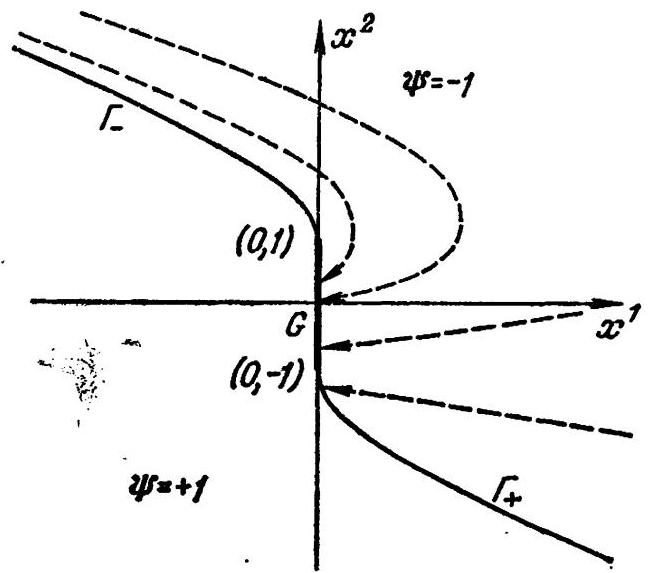
\includegraphics[max width=0.6\textwidth]{images/bo_d547k8bef24c73bgfcg0_151_706_677_656_573_0.jpg}
\end{center}
\hspace*{3em} 

Рис. 2.1. Кривая переключения и синтез опти- мальных управлений для системы из ехでи, \({\dot{x}}^{2} =  - {x}^{2} + u,\;\left| u\right|  \leq  1;\;\) целевое множество \(G\) ; \({x}^{1} = 0,\left| {x}^{2}\right|  \leq  1\) .

Пример 2. Рассмот- рим автономную управляе- мую систему в \({R}^{3}\)

\[
\ddot{x} = u
\]

HJIM

\[
\left( \mathcal{L}\right) {\dot{x}}^{1} = {x}^{2},{\dot{x}}^{2} = {x}^{3},
\]

\[
{\dot{x}}^{3} = u
\]

с ограничивающим множе- ством \(\Omega  : \left| u\right|  \leq  1\) в \({R}^{1}\) . Tpe- буется найти оптимальное по быстродействию управ- ление, переводящее систему в начало координат. Теоре- мы 8 и 17 гарантируют существование такого управления для любого начального состояния из \({R}^{3}\) , a следствие 3 из теоремы 19 показывает, что это опти- мальное управление и есть единственное экстремальное управле- ние, переводящее систему в начало координат.

Для построения кривой переключений снова применим метод «попятного» движения. Запишем систему 𝒳 и сопряженную сис- тему при обратном отсчете времени:

\[
{\dot{x}}^{1} =  - {x}^{2},\;{\dot{x}}^{2} =  - {x}^{3},\;{\dot{x}}^{3} =  - u,\text{ где }u = \operatorname{sgn}{\eta }_{3}\left( t\right) ,
\]

\[
{\dot{\eta }}_{1} = 0,\;{\dot{\eta }}_{2} = {\eta }_{1},\;{\dot{\eta }}_{3} = {\eta }_{2}.
\]

3 аметим, что \({\eta }_{3} = 0\) , tax что \({\eta }_{3}\left( t\right)  = {\eta }_{30} + {\eta }_{20}t + {\eta }_{10}{t}^{2}/2\) ; поэтому каждое экстремальное управление имеет не более двух переклю- чений, соответствующих нулям функции \({\eta }_{2}\left( t\right)\) , pacположенным на положительной полуоси. Определим кривую Г+ как траекторию, исходящую из начала координат при \(u =  + 1\) ,т. e. \({x}^{1} =  - \frac{{t}^{3}}{6}\) , \({x}^{2} = \frac{{t}^{2}}{2},{x}^{3} =  - t\) при \(t > 0\) . Поскольку начальные условия пди, \({\eta }_{10},{\eta }_{20}\) , \({\eta }_{30}\) можно выбрать так,чтобы \({\eta }_{3}\left( t\right)  > 0\) при \(0 < t < {t}_{1},{\eta }_{s}\left( t\right)  < 0\) при \({t}_{1} < t < {t}_{2} \leq   + \infty\) и \({\eta }_{3}\left( t\right)  > 0\) при \(t > {t}_{2}\) для произвольных \(0 < {t}_{1} < {t}_{2} \leq   + \infty\) ,то каждая точка кривой \({\Gamma }_{ + }\) может оказаться точкой переключения -управления с и = — 1 на управление и = +1 для экстремального управления, переводящего систему в начало координат вдоль траектории \({\Gamma }_{ + }\) .

Для каждой точки \({\overline{\Gamma }}_{ + }\) , ompeдeляемой некоторым значением \(t > 0\) ,вычисляем решения системы дифференциальных уравнений с обратным отсчетом времени, соответствующие значению управ- ления и == 1. Обозначая независимую переменную через s (s ≥ 0), запишем эти решения в виде

\[
{x}^{1} = \frac{{s}^{3}}{6} - \frac{{s}^{2}t}{2} - \frac{s{t}^{2}}{2} - \frac{{t}^{3}}{6},\;{x}^{2} =  - \frac{{s}^{2}}{2} + {st} + \frac{{t}^{2}}{2},\;{x}^{3} = s - t.
\]

Для \(t > 0,s \geq  0\) эти уравнения определяют поверхность переклю- чений \({W}_{ - }\) , содepжащую кривую переключений \({\Gamma }_{ + }\) .

Определим теперь кривую Г\_ как траекторию, исходящую из начала координат и соответствующую управлению и е — 1:

\[
{x}^{1} = \frac{{t}^{3}}{6},\;{x}^{2} =  - \frac{{t}^{2}}{2},\;{x}^{3} = t\text{ при }t > 0.
\]

Теперь интегрируем нашу систему с обратным отсчетом времени, используя в качестве начальной точки любую точку Г\_, а в ка- честве управления \(u =  + 1\) . Тогда получим поверхность переклю- чений \({W}_{ + }\) :

\[
{x}^{1} = \frac{{t}^{3}}{6} + \frac{{t}^{2}s}{2} + \frac{t{s}^{2}}{2} - \frac{{s}^{3}}{6},\;{x}^{2} =  - \frac{{t}^{2}}{2} - {ts} + \frac{{s}^{2}}{2},{x}^{3} = t - s
\]

при \(s \geq  0,t > 0\) . Полная поверхность переключений \(W = {W}_{ - } \cup  {W}_{ + }\) будет содержать полную кривую переключений \(\Gamma  = {\Gamma }_{ + } \cup  {\Gamma }_{ - }\) . Пока- жем, что поверхность \(W\) разбивает пространство \({R}^{3}\) , a кривая \(\Gamma\) разбивает поверхность \(W\) (в \(\Gamma\) включается начало координат). Действительно, W есть однозначная функция переменных ( \({x}^{1},{x}^{3}\) ). Чтобы проверить это, возьмем произвольную точку ( димся, что единственное значение параметров \(\left( {s,t}\right)\) определяет точку ( \({\bar{x}}^{1},{\bar{x}}^{2},{\bar{x}}^{3}\) ) на поверхности W.

На \({W}_{ - }\) имеем

\[
{x}^{1} = \frac{{\left( {x}^{3}\right) }^{3}}{6} - s{t}^{2}\;\left( {s \geq  0,t > 0}\right) ,
\]

a На \({W}_{ + }\)

\[
{x}^{1} = \frac{{\left( {x}^{3}\right) }^{3}}{6} + s{t}^{2}\;\left( {s \geq  0,t > 0}\right) .
\]

Таким образом, если \(\bar{x} = {\left( {\bar{x}}^{3}\right) }^{3}/6\) , то \(s = 0\) . Если \({\bar{x}}^{1} < 0\) , то следует выбрать точку на \({\Gamma }_{ - }\) ,где \(\overline{{x}^{2}} = {\left( \overline{{x}^{3}}\right) }^{2}/2\) ; в противном случае выби- раем точку на \({\Gamma }_{ + }\) ,где \({\bar{x}}^{2} =  - {\left( \overline{{x}^{3}}\right) }^{2}/2\) . Если \({\bar{x}}^{1} < {\left( \overline{{x}^{3}}\right) }^{3}/6\) ,то ищем точку на \({W}_{ - }\) , если же \(\overline{{x}^{1}} > {\left( \overline{{x}^{3}}\right) }^{3}/6\) , to на \({W}_{ + }\) . Пусть,например, \({x}^{1} < {\left( {x}^{3}\right) }^{3}/6\) ,тогда ищем корень \(t > 0\) уравнения

\[
s{t}^{2} + \left\lbrack  {{x}^{1} - \frac{{\left( \overline{{x}^{3}}\right) }^{8}}{6}}\right\rbrack   = 0\text{ или }\left( {\overline{{x}^{3}} + t}\right) {t}^{2} + \left\lbrack  {\overline{{x}^{1}} - \frac{{\left( \overline{{x}^{3}}\right) }^{3}}{6}}\right\rbrack   = 0.
\]

Поскольку левая часть этого уравнения представляет собой мно- гочлен третьей степени от \(t\) и в точке \(t = 0\) касательная к его графику горизонтальна, то легко видеть, что этот многочлен имеет лишь один положительный корень. Аналогичным образом можно показать, что и на W+ имеется лишь одна точка, в которой \({\bar{x}}^{1} > {\left( {\bar{x}}^{3}\right) }^{3}/6\)

Таким образом, поверхность W разбивает пространство R³ на две области: \({M}_{ + }\) ,где \({x}^{2} \rightarrow   + \infty ,u{M}_{ - }\) ,где \({x}^{2} \rightarrow   - \infty\) . Поскольку кривая \({\Gamma }_{ - }\) соответствует границе W\_, где параметры принимают значения \(t = 0,s > 0\) и,аналогично, \({\Gamma }_{ + }\) соответствует границе \({W}_{ + }\) , то ясно, что \(\Gamma\) разбивает поверхность \(W\) на две части.

Если начальная точка ( \({x}_{0}^{1},{x}_{0}^{2},{x}_{0}^{3}\) ) лежит в \({M}_{ + }\) ,то мы приме- няем управление \(u =  + 1\) , noka траектория не достигнет \({W}_{ + }\) . Затем производим переключение, и используем управление и — 1, пока не достигнем \({\Gamma }_{ + }\) ,затем переключаемся на \(u =  + 1\) ,и вдоль \({\Gamma }_{ + }\) пе- реводим систему в начало координат. Если начальная точка при- надлежит М\_, то всюду в переключениях будут обратные знаки. Таким образом, синтезирующая функция имеет вид

\[
\Psi \left( {{x}^{1},{x}^{2},{x}^{3}}\right)  = \left\{  \begin{array}{lll}  + 1 & \mathrm{\;B} & {M}_{ + }, \\   - 1 & \mathrm{B} & {M}_{ - }, \\   - 1 & \mathrm{{На}} & {W}_{ - } -  - {\Gamma }_{ + }, \\   + 1 & \mathrm{{На}} & {W}_{ + } - {\Gamma }_{ - }, \\   + 1 & \mathrm{{На}} & {\Gamma }_{ + }, \\   - 1 & \mathrm{{На}} & {\Gamma }_{ - }. \end{array}\right.
\]

Пример 3. Рассмотрим автономную управляемую систему в R", определяемую уравнением

\[
{x}^{\left( n\right) } + {a}_{1}{x}^{\left( n - 1\right) } + {a}_{2}{x}^{\left( n - 2\right) } + \ldots  + {a}_{n}x = u,
\]

c orpaничением на управления \(\left| u\right|  \leq  1\) в \({R}^{1}\) . Tpeбуется перевести систему из начального состояния (и, и, и) и (i) и (i) и (ii) и (ii) минимальное время и в дальнейшем удерживать ее в этом состоя- нии. Соответствующая система дифференциальных уравнений в R" будет иметь вид

\[
\left( \mathcal{L}\right)
\]

\[
\dot{\mathbf{x}} = A\mathbf{x} + {bu},
\]

где

\begin{center}
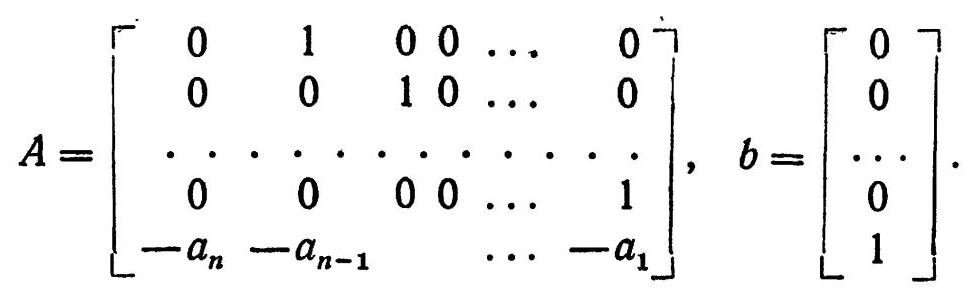
\includegraphics[max width=0.8\textwidth]{images/bo_d547k8bef24c73bgfcg0_154_349_209_973_288_0.jpg}
\end{center}
\hspace*{3em} 

Легко видеть, что множество core \(\left( {{x}^{1} = 0}\right)\) есть начало координат; оно является целевым множеством нашей задачи. Система 𝒳 вполне управляема, а следовательно, нормальна. В этом случае область нуль-управляемости € является открытым связным под- множеством \({R}^{n}\) и мы предположим,что начальная точка х, ее с. Тогда существует единственное экстремальное управление, пере- водящее систему из х, в начало координат, и оно является опти- мальным управлением и* (t) на интервале 0≤ t<t+ \textbackslash t соответст- вующим решением х* (t) и сопряженным решением η* (t).

Здесь под \({\eta }^{ * }\left( t\right)\) понимается нетривиальное решение системы

\[
\dot{\mathbf{\eta }} =  - {\eta A}\text{ или }{\dot{\mathbf{\eta }}}^{\prime } =  - {A}^{\prime }{\mathbf{\eta }}^{\prime },\text{ где }\eta  = \left( {{\eta }_{1},{\eta }_{2},\ldots ,{\eta }_{n}}\right) .
\]

Nmeem

\[
{\eta }_{1} = {a}_{n}{\eta }_{n},\;{\eta }_{2} =  - {\eta }_{1} + {a}_{n - 1}{\eta }_{n},
\]

\[
{\eta }_{n - 1} =  - {\eta }_{n - 2} + {a}_{2}{\eta }_{n},{\eta }_{n} =  - {\eta }_{n - 1} + {a}_{1}{\eta }_{n}.
\]

Последовательно исключая переменные, получим дифференциальное уравнение относительно \({\eta }_{n}\left( t\right)\) :

\[
{\eta }_{n}^{\left( n\right) } - {a}_{1}{\eta }_{n}^{\left( n - 1\right) } + {a}_{2}{\eta }_{n}^{\left( n - 2\right) } - {a}_{3}{\eta }_{n}^{\left( n - 3\right) } + \cdots  + {\left( -1\right) }^{n}{a}_{n}{\eta }_{n} = 0.
\]

Оптимальное управление удовлетворяег принципу максимума

\[
{\eta }^{ * }\left( t\right) b{u}^{ * }\left( t\right)  = \max {\eta }^{ * }\left( t\right) {bu}
\]

Так ЧТО

\[
{u}^{ * }\left( t\right)  = \operatorname{sgn}{\eta }_{n}\left( t\right) \text{ почтн всюдуна интервале }0 \leq  t \leq  {t}^{ * }\text{ . }
\]

Заметим, однако, что при рассмотрении общего вида системы \(n\) -го порядка практическое применение метода кривых переклю- чений и изучение геометрии множества € сопряженно с большим трудностями.

Эти трудности в исследовании кривых переключений и запоми- нании их описаний (в вычислительных устройствах) указывают на нецелесообразность применения описанных методов для управляе- мых систем порядка выше третьего. В приложении А мы опишем метод, позволяющий непосредственно определять оптимальное управление системы без рассмотрения этих геометрических тонкостей.

Однако, хотя в общем случае полное описание кривой пере- ключений для систем высокого порядка весьма затруднительно, существуют два важных случая, для которых легко установить некоторые свойства, относящиеся к переключениям управлений системы.

Теорема 20. Рассмотрим автономную линейную систему в R":

(L)
\[
\dot{x} = {Ax} + {bu},
\]

с ограничивающим множеством Ω: | и | ≤ 1 в R . Предположим, что система 2 вполне управляема, а значит, нормальна.

Если все собственные значения матрицы A действительны, то любое экстремальное управление имеет не более n-1 переключе- ний на полуоси 0 ≤ t < ∞.

Если все собственные значения матрицы А имеют ненулевую мнимую часть, то любое экстремальное управление имеет беско- нечное число переключений на полуоси 0≤t <0 . Таким образом, для любого положительного числа N > 0 существует такое началь- ное состояние \({x}_{0} \in  {R}^{n}\) ,для которого соответствующее оптимальное управление, переводящее систему из х, в начало координат, имеет более N переключений.

Доказательство. Поскольку система 8 вполне управляе- ма, то по теореме 7 можно ввести такую систему координат, в которой матрицы коэффициентов системы Q примут такой вид:

\[
A = \left[ \begin{array}{cccccc} 0 & 1 & 0 & 0 & \ldots & 0 \\  0 & 0 & 1 & 0 & \ldots & 0 \\  \vdots & \vdots & \vdots & \vdots & & \vdots \\  0 & 0 & 0 & 0 & \ldots & 1 \\   - {a}_{n} &  - {a}_{n - 1} & & \ldots &  - {a}_{1} & \end{array} \right]  ,\;b = \left[ \begin{array}{c} 0 \\  0 \\  \vdots \\  0 \\  1 \end{array} \right]  .
\]

Тогда систему 𝒳 можно описать с помощью одного уравнения \(n\) -го порядка:

\[
{x}^{\left( n\right) } + {a}_{1}{x}^{\left( n - 1\right) } + \ldots  + {a}_{n}x = u,\;\left| u\right|  \leq  1.
\]

Экстремальное управление \(u\left( t\right)\) имеегвид

\[
u\left( t\right)  = \operatorname{sgn}\eta \left( t\right)
\]

где \(\eta \left( t\right)\) есть последняя компонента нетрнвнального рещеня системы

\[
\left[ \begin{array}{c} {\dot{\eta }}_{1} \\  \vdots \\  {\dot{\eta }}_{n} \end{array} \right]   =  - {A}^{\prime }\left[ \begin{array}{c} {\eta }_{1} \\  \vdots \\  {\eta }_{n} \end{array} \right]
\]

Легко показать, что функция \({\eta }_{n}\left( t\right)\) является решеннем уравнения

\[
{\eta }^{\left( n\right) } - {a}_{1}{\eta }^{\left( n - 1\right) } + {a}_{2}{\eta }^{\left( n - 2\right) } - \ldots  + {\left( -1\right) }^{n}{a}_{n}\eta  = 0.
\]

Собственные значения \(\left\{  {{\lambda }_{1},{\lambda }_{2},\ldots ,{\lambda }_{r}}\right\}\) матрицы — \({A}^{\prime }\) равняются собственным значениям матрицы A, взятым с обратными знаками, следовательно, они будут действительными или комплексными одновременно с собственными значениями матрицы A.

Предположим, что все собственные значения матрицы A дейст- вительны. Тогда

\[
\eta \left( t\right)  = {P}_{1}\left( t\right) {e}^{{\lambda }_{1}t} + \ldots  + {P}_{r}\left( t\right) {e}^{{\lambda }_{r}t},
\]

где действительные многочлены \({P}_{j}\left( t\right)\) имеют степени ≤ \({n}_{j} - 1\) , а \({n}_{j}\) -кратность собственного значения \({\lambda }_{j}\left( {1 \leq  j \leq  r}\right)\) . Но \({n}_{1} + {n}_{2} + \ldots\) ... + \({n}_{r} = n\) и в силу известного свойства экспоненциальных многочленов (см. ниже упражнение 13) функция \(\eta \left( t\right)\) может иметь не более \(n - 1\) действительных нулей (— \(\infty  < t < \infty\) ). Отсюда следует, что экстремальное управление и (t) имеет не более n-1 переключения на \(0 \leq  t < \infty\) .

Предположим теперь, что все собственные значения матрицы \(A\) имеют ненулевые мнимые части, а значит, то же самое верно и для собственных значений \({\lambda }_{j} = {\alpha }_{j} + i{\beta }_{j}\) матрицы — \({A}^{\prime }\) . В этом случае

\[
\eta \left( t\right)  = {e}^{{\alpha }_{1}t}\left\lbrack  {{P}_{1}\left( t\right) \cos {\beta }_{1}\left( t\right)  + {Q}_{1}\left( t\right) \sin {\beta }_{1}t}\right\rbrack   + \ldots
\]

\[
\ldots  + {e}^{{\alpha }_{r}t}\left\lbrack  {{P}_{r}\left( t\right) \cos {\beta }_{r}t + {Q}_{r}\left( t\right) \sin {\beta }_{r}t}\right\rbrack  ,
\]

где \({P}_{1}\left( t\right) ,{Q}_{1}\left( t\right) ,\ldots ,{P}_{r}\left( t\right) ,{Q}_{r}\left( t\right)\) —действительные многочлены, не все равные нулю. Для простоты обозначим через а, наиболь. шее из чисел \({\alpha }_{1},{\alpha }_{2},\ldots ,{\alpha }_{r}\) ,входящих с ненулевыми коэффициен. тами в выражение для \(\eta \left( t\right)\) . Тогда

\[
\eta \left( t\right)  = {e}^{{\alpha }_{1}t}{t}^{k}\mathop{\sum }\limits_{{j = 1}}^{r}\left( {{a}_{j}\cos {\beta }_{j}t + {b}_{j}\sin {\beta }_{j}t}\right)  + R\left( t\right) .
\]

Здесь k ≥ 0 и тригонометрическая сумма

\[
T\left( t\right)  = \mathop{\sum }\limits_{{j = 1}}^{r}\left( {{a}_{j}\cos {\beta }_{j}t + {b}_{j}\sin {\beta }_{j}t}\right)
\]

не равняется тождественно нулю. Остаточный член \(R\left( t\right)\) таков,что

\[
\mathop{\lim }\limits_{{t \rightarrow  \infty }}{e}^{-{\alpha }_{1}t}{t}^{-k}R\left( t\right)  = 0.
\]

Заметим, что \(T\left( t\right)\) является конечной тригонометрической сум- мой с нулевым средним значением на интервале 0</t<∞. Кроме того, для некоторого 8 > 0 найдется такое \(L > 0\) ,что сумма \(T\left( t\right)\) принимает значения, большие, чем 8 и меньшие, чем —в, на каж- дом интервале длины L. (Это следует из теории почти-периоди- ческих функций, или из непосредственного изучения выражения \(T\left( t\right)\) .) Пусть \(\bar{t} > 0\) таково,что

\[
\left| {{e}^{-{\alpha }_{1}t}{t}^{-k}R\left( t\right) }\right|  < \frac{\varepsilon }{2}
\]

для \(t \geq  \bar{t}\) . Тогда функция

\[
{e}^{-{\alpha }_{1}t}{t}^{-k}\eta \left( t\right)  = T\left( t\right)  + {e}^{-{\alpha }_{1}t}{t}^{-k}R\left( t\right)
\]

должна иметь нуль в каждом интервале \({t}_{1} \leq  t \leq  {t}_{1} + L\) при \({t}_{1} > \bar{t}\) . Tem самым функция \(\eta \left( t\right)\) имеет бесконечное число нулей, а управле- ние \(u\left( t\right)\) имеет бесконечное число переключений на интервале \(0 \leq  t < \infty\) .

Поскольку оптимальное управление для заданного начального состояния \({x}_{0}\) получается из экстремального управления с помощью попятного движения из начала координат, то существуют такие точки \({x}_{0} \in  {R}^{n}\) ,для которых оптимальное управление и*(t) на ин- тервале 0≤た≤t* имеет число переключений, большее наперед заданного числа N. Теорема доказана.

Другой метод синтеза оптимального управления основан на применении изохронных гиперповерхностей в \({R}^{n}\) . Пусть T (x)-ми- нимальное время, требуемое для перевода системы из начального состояния \(x\) в целевое множество; тогда геометрическое место точек в \({R}^{n}\) ,для которых

\[
T\left( x\right)  = t\text{ при }t \geq  0,
\]

называется изохронной гиперповерхностью, отвечающей значению параметра t. Вдоль оптимальной траектории х*(t) на интервале \({t}_{0} \leq  t \leq  0\) имеем

и

\[
T\left( {{x}^{ * }\left( t\right) }\right)  =  - t
\]

\[
\nabla T\left( {{x}^{ * }\left( t\right) }\right) {\dot{x}}^{ * }\left( t\right)  =  - 1
\]

всюду, где существуют вектор-строка ∇Т = grad Т и производная \({x}^{ * }\left( t\right)\) .

Ниже мы покажем, что вектор— ∇Т (х)можно использовать вместо сопряженного решения η(t) при синтезе оптимального управле- ния \({u}^{ * }\left( t\right)\) . Чтобы упростить доказательство этого факта, будем предполагать, что целевое множество G есть начало координат, и что существует единственное экстремальное управление, перево- дящее систему из начального состояния в начало координат, как в следствии 3 из теоремы 19.

T e o p e ма 21. Рассмотрим автономную линейную систему в R":

(2)
\[
\dot{x} = {Ax} + {Bu},
\]

с компактным ограничивающим множеством Ω⊂R’ подержащим внутри себя точку и =0. Предположим, что система \{Q, Ω\} нор- мальна на любом интервале, а область нуль-управляемости совпа- дает со всем пространством R". Пусть T(x)— минимальное время, требуемое для перевода системы из начального состояния хе к’во п в начало координат. Тогда Т(х) непрерывна в R", а изохронные

\section*{гиперповерхности}

\[
T\left( x\right)  = t\;\partial n/\partial x/x\partial {020}\;t > 0
\]

образуют семейство замкнутых выпуклых гиперповерхностей, моно- тонно и неограниченно «раздувающихся» с ростом t.

Доказательство. Рассмотрим множество достижимости \(K\left( {t}_{1}\right)\) для \({t}_{1} > 0\) ,начального состояния \({x}_{0} = 0\) и управлений из \(\Omega\) . Каждое из множеств K(t,1) является компактным строго выпук- лым, причем K(t, i)ск K(t, d) для 0</i<t> </i </i. замечания после теоремы 3, а также упражнение 4 к разделу 3). Мы докажем, что reometрическое место точек, для которых \(T\left( x\right)  = {t}_{1}\) ,в точности совпадает с границей множества \(K\left( {t}_{1}\right)\) в \({R}^{n}\) .

Пусть \({x}_{1} \in  \partial K\left( {t}_{1}\right)\) так, что существует лишь одно экстремальное управление \({u}_{1}\left( t\right)\) на интервале 0 ≤ t ≤ t, переводящее систему из состояния \({x}_{0}\) в состояние \({x}_{1}\) . Поскольку \({u}_{1}\left( {-t}\right)\) есть оптимальное управление, переводящее систему из \({x}_{1}\) в \({x}_{0}\) , to \(T\left( {x}_{1}\right)  = {t}_{1}\) . Oбратно, точка \({x}^{ * }\) ,для которой \(T\left( {x}^{ * }\right)  = {t}_{1}\) ,является концом оптимальной траектории \({x}^{ * }\left( t\right)\) , no которой система переходит из \({x}_{0}\) в \({x}^{ * }\left( {t}_{1}\right)  = {x}^{ * }\) . Таким образом, точка х* принадлежит границе множества K(t,), и мы показали, что изохронная поверхность \(T\left( x\right)  = {t}_{1}\) есть не что иное,как замкнутая выпуклая граница множества K(t) в R". Заметим, что изохронные гиперповерхности семейства

\[
T\left( x\right)  = {t}_{1}\text{ для }{t}_{1} > 0
\]

не пересекаются, и каждая из них замыкается вокруг начала ко- ординат. Кроме того, эти гиперповерхности монотонно и неогра- ниченно расширяются с ростом \({t}_{1}\) от 0 до ∞,поскольку также меняются множества \(K\left( {t}_{1}\right)\) .

Для доказательства непрерывности вектор-функции \(T\left( x\right)\) в \({R}^{n}\) положим \(T\left( {x}_{1}\right)  = {t}_{1}\) . Далее, для некоторого ε> 0 рассмотрим слой, заключенный между гиперповерхностями \(T\left( x\right)  = {t}_{1} - \varepsilon\) и \(T\left( x\right)  = \; = {t}_{1} + \varepsilon\) . (Если \({x}_{1} = 0\) , то \(T\left( {x}_{1}\right)  = 0\) и рассуждения не меняются.) Тогда для достаточно малого δ> 0 окрестность \(\left| {x - {x}_{1}}\right|  < \delta\) лежит внутри этого слоя, а значит, \(\left| {T\left( x\right)  - {t}_{1}}\right|  < \varepsilon\) . Таким образом, \(T\left( x\right)\) непрерывна в точке \({x}_{1}\) , a следовательно,в каждой точке \({R}^{n}\) . Teo- рема доказана.

Cледствие. Предположим, что T (х) ∈ \({C}^{1}\) в некотором от- крытом подмножестве 6—R’, не пересекающемся с кривой пере- ключений автономной системы

(Y)
\[
\dot{x} = {Ax} + {Bu}.
\]

Toe∂ \(a\)

\[
\mathop{\max }\limits_{{u \in  \Omega }}\left\lbrack  {-\nabla T\left( x\right) }\right\rbrack  \left\lbrack  {{Ax} + {Bu}}\right\rbrack   = 1\text{ в }0.
\]

Ecru, kpome mozo, ozparuyusaowlee MHONCECMBO \(\Omega\) ecmb m-MePHbli \({\kappa y}{6}^{\prime }\left| {u}^{j}\right|  \leq  1,\) mo для каждой точки \(x \in  \mathcal{C}\) onmимальное управление имеет значение \(\Psi \left( x\right)\) ,где

\[
\Psi \left( x\right)  =  - \operatorname{sgn}\left\lbrack  {\nabla T\left( x\right) B}\right\rbrack  .
\]

Доказательство. Пусть х*(*) (0 ≤ t ≤ t*) — оптимальная траектория, по которой движется система, переходя из точки и, с б в начало координат под воздействием управления и*(t). Тогда

\[
T\left( {{x}^{ * }\left( t\right) }\right)  =  - t
\]

H, 3Ha4HT,

\[
\nabla T\left( {{x}^{ * }\left( t\right) }\right) {\dot{x}}^{ * }\left( t\right)  = \nabla T\left( {{x}^{ * }\left( t\right) }\right) \left\lbrack  {A{x}^{ * }\left( t\right)  + B{u}^{ * }\left( t\right) }\right\rbrack   =  - 1
\]

при \(0 \leq  t \leq  {t}_{1}\) и \({x}^{ * }\left( t\right)  \subset  6\) . Таким образом, вектор \(\nabla T\left( {x}_{1}\right)\) на мно- жестве 6 не обращается в нуль, а значит, определяет вектор внешней нормали к гиперплоскости, касательной к изохронной гиперповерхности в точке \({x}_{1}\) . Отсюда ясно,что вектор \(\nabla T\left( {x}_{1}\right)\) отличается лишь на положительный множитель от вектора η(t*) сопряженного решения, соответствующего оптимальному управле- нию \({u}^{ * }\left( {{t}^{ * } - t}\right)\) , которое переводит систему из точки х, 0 =0 в точку х,. Тогда вектор — Ви* (О) имеет максимальную возможную проекцию на направление \(\nabla T\left( {x}_{1}\right)\) ,или

\[
- \nabla T\left( {x}_{1}\right) B{u}^{ * }\left( 0\right)  = \mathop{\max }\limits_{{u \in  \Omega }}\left\lbrack  {-\nabla T\left( {x}_{1}\right) {Bu}}\right\rbrack  .
\]

Orcioда

\[
\mathop{\max }\limits_{{u \in  \Omega }}\left\{  {-\nabla T\left( {x}_{1}\right) \left\lbrack  {A{x}_{1} + {Bu}}\right\rbrack  }\right\}   =  - \nabla T\left( {x}_{1}\right) \left\lbrack  {{Ax} + B{u}^{ * }\left( 0\right) }\right\rbrack   = 1.
\]

Поэтому в каждой точке \(x \in  \mathcal{6}\) имеем

\[
\mathop{\max }\limits_{{u \in  \Omega }}\left\lbrack  {-\nabla T\left( x\right) }\right\rbrack  \left\lbrack  {{Ax} + {Bu}}\right\rbrack   = 1.
\]

Наконец, рассмотрим в качестве Ω m-мерный куб | и'| < 1. Тогда оптимальное управление, переводящее систему из точки \({x}_{0} = 0\) в точку \({x}_{1} \in  \mathcal{C}\) ,будет иметь вид

\[
{u}^{ * }\left( {{t}^{ * } - t}\right)  = \operatorname{sgn}\left\lbrack  {-\eta \left( t\right) B}\right\rbrack
\]

и поэтому в каждой точке \({x}_{1} \in  \mathcal{C}\)

\[
\Psi \left( {x}_{1}\right)  = \operatorname{sgn}\left\lbrack  {-\eta \left( {t}^{ * }\right) B}\right\rbrack   =  - \operatorname{sgn}\left\lbrack  {\nabla T\left( {x}_{1}\right) B}\right\rbrack  ,
\]

что и требовалось доказать.

Из этого следствия вытекает метод синтеза оптимального управления \({u}^{ * }\left( t\right)\) ,использующий изохронную функцию \(T\left( x\right)\) . Сформулируем его следующим образом:

1. Найти явно функцию \(T\left( x\right)\) , peшив систему дифференциаль- ных уравнений в частных производных:

\[
\nabla T\left\lbrack  {{Ax} + B}\right\rbrack   =  - 1\text{ в }{M}_{ + },
\]

\[
\nabla T\left\lbrack  {{Ax} - B}\right\rbrack   =  - 1\text{ в }{M}_{ - }.
\]

Здесь под Ω понимается интервал \(\left| u\right|  \leq  1\) , a \({M}_{ + }\) и \({M}_{ - } -\) области, где оптимальное управление принимает значения соответственно +1 и -1.

2. Определнть синтезирующуго функцию \(\Psi \left( x\right)\) :

\[
\Psi \left( x\right)  =  - \operatorname{sgn}\left\lbrack  {\nabla T\left( x\right) B}\right\rbrack  \text{ для }x \in  {M}_{ + } \cup  {M}_{ - }.
\]

Этот метод, однако, содержит все те трудности, с которыми мы сталкивались в методе кривых переключений. Действительно, ведь для определения областей М и и меобходимо найти кривую переключений. Затем придется решать задачу Коши для уравне- ний в частных производных относительно \(T\left( x\right)\) ,где краевые усло- вия есть значения функции \(T\left( x\right)\) ,вычисленные на кривой пере- ключений. Оптимальные траектории являются характеристиками этих уравнений в частных производных, поэтому для вычисле- ния \(T\left( x\right)\) должны быть вычислены и оптимальные траектории.

Метод изохронных поверхностей интересен теоретически; иногда он представляет интерес и с вычислительной точки зрения, однако было бы затруднительно дать достаточно полное и общее изложение этого метода.

Мы завершим эту главу об управлении линейными системами доказательством того факта, что минимальное оптимальное время t* и оптимальное управление и « (t) в некотором смысле непрерывно зависят от всех условий задачи управления \(\{ \mathcal{L},\Omega ,{x}_{0},{t}_{0},G\}\) . Эта непрерывная зависимость позволяет заменять сложные физические задачи их идеализированными математическими моделями, и по- лучать при этом достаточно близкие к действительности прибли- женные оптимальные управления. Для простоты будем рассматри- вать автономные системы с началом координат в качестве целевого множества G и многогранную область Ω в качестве ограничиваю- щего множества. Поскольку ребра многогранника Ω играют важ- ную роль в условии нормальности, мы обозначим через Ед мно- жество всех единичных векторов в \({R}^{m}\) ,параллельных ребрам Ω (или самому Ω, если это отрезок).

Teopeма 22. Рассмотрим автономную линейную систему в R":

(Y)
\[
x = {Ax} + {Bu},
\]

с выпуклым ограничивающим многогранником Ω⊂R", содержащим \(u = 0\) внутри себя. Пусть выполняется условие нормальности:

\[
\text{ seкmopbι Bw, ABw, . . ., }{A}^{n - 1}{Bw}
\]

линейно независимы для любого шес Ео. Пусть далее х,—начальная точка из области C нуль-управляемости, а и*(t) ⊂ Ω (0 ≤ t ≤ t*) — оптимальное управление, переводящее систему из состояния х, в начало координат вдоль траектории х* (t).

Рассмотрим возмущенную автономную систему в R":

\[
\left( \widehat{\mathcal{L}}\right)
\]

\[
\dot{x} = \widehat{A}x + \widehat{B}u,
\]

с выпуклым ограничивающим многогранником Ω⊂R™ и начальным состоянием до. Тогда для любого ε>0 существует такое δ>0, что из неравенства

\[
\left| {A - \widehat{A}}\right|  + \left| {B - \widehat{B}}\right|  + \left| {{x}_{0} - {\widehat{x}}_{0}}\right|  + \operatorname{dist}\left( {\Omega ,\widehat{\Omega }}\right)  + \operatorname{dist}\left( {{E}_{\Omega },{E}_{\widehat{\Omega }}}\right)  < \delta
\]

следует, что точка х, лежит в области нуль-управляемости 6 системы 29, что система \{\$, Ω, χ, нормальна, и что сущест- вует единственное оптимальное управление йч (не С д на интервале \(0 \leq  t \leq  {\widehat{t}}^{ * }\) , nepеводящее систему из состояния ховори-ол нат вдоль траектории ль" (t).

Далее,

\(u\)

\[
\left| {{t}^{ * } - {\widehat{t}}^{ * }}\right|  < \varepsilon
\]

\[
\left| {{x}^{ * }\left( t\right)  - {\widehat{x}}^{ * }\left( t\right) }\right|  < \varepsilon \;{\text{ н }\text{ а }}\;0 \leq  t \leq  {\tau }^{ * } = \min \left\lbrack  {{t}^{ * },{\widehat{t}}^{ * }}\right\rbrack  ,
\]

\[
{\int }_{0}^{{\tau }^{ * }}\left| {{u}^{ * }\left( t\right)  - {\widehat{u}}^{ * }\left( t\right) }\right| {dt} < \varepsilon
\]

Доказательство. Поскольку всякий определитель непре- рывно зависит от своих элементов, то существует б, >0, такое, что из неравенства

\[
\mathcal{L} - \widehat{\mathcal{L}}\left|  \equiv  \right| A - \widehat{A}\left| +\right| B - \widehat{B}\left| +\right| {x}_{0} - {\widehat{x}}_{0}| + \operatorname{dist}\left( {\Omega ,\widehat{\Omega }}\right)  +
\]

\[
+ \operatorname{dist}\left( {{E}_{\Omega },{E}_{\widehat{\Omega }}}\right)  < {\delta }_{1}
\]

следует, что

\[
\det \left\lbrack  {\widehat{B}\widehat{w},\widehat{A}\widehat{B}\widehat{w},\ldots ,{\widehat{A}}^{n - 1}\widehat{B}\widehat{w}}\right\rbrack   \neq  0\text{ для }\widehat{w} \in  {E}_{\widehat{\Omega }}.
\]

Выберем теперь δ, > 0 столь малым, чтобы существовала компакт- ная кубическая окрестность \(N\) управления и е=О, лежащая вну- три всех тех Ω, для которых dist \(\left( {\Omega ,\widehat{\Omega }}\right)  \leq  {\delta }_{1}\) . Мы будем рассма- тривать лишь те задачи \{ \(\widetilde{\mathcal{L}},\widehat{\Omega },{\widehat{x}}_{0}\) \},для которых | \(\mathcal{L} - \widetilde{\mathcal{L}} \mid   < {\delta }_{1}\) ; каждая из них является нормальной, вполне управляемой, и имеет в качестве области нуль-управляемости некоторое открытое мно- жество \(\widehat{\mathcal{C}} \subset  {R}^{n}\) .

Возьмем любое ε из интервала 0 < ε < 1 и пусть \& (ε/2, N)⊂R" есть множество тех точек, в которые система может быть переве- дена из начала координат за время ε/2 с помощью управлений \(u\left( t\right)  \subset  N\) вдоль траекторий, являющихся решениями системы £?. В силу управляемости системы Ф каждое из множеств Ф(ε/2, N) должно содержать вписанный шар радиуса r>0 с центром в на- чале координат. Небольшое изменение коэффициентов )2 приводит к некоторому изменению множества \& (ε/2, N), причем для нового выпуклого множества радиус вписанного шара будет больше, чем \(\widehat{r} - \xi\) для заданного \(\xi  > 0\) . Таким образом, \(\widehat{r}\) является полунепре- рывной снизу функцией матриц А и В, а поэтому г имеет поло- жительный минимум \({r}_{\varepsilon } > 0\) при \(\left| {A - \widehat{A}}\right|  + \left| {B - \widehat{B}}\right|  \leq  {\delta }_{1}\) .

Пусть \({u}^{ * }\left( t\right)  \subset  \Omega \left( {0 \leq  t \leq  {t}^{ * }}\right)\) - оптимальное управление, перево- дящее систему из состояния \({x}_{0}\) в начало координат вдоль реше- ния \({x}^{ * }\left( t\right)\) системы \(\mathcal{L}\) ,и пусть \(\widehat{u}\left( t\right)  \subset  \widehat{\Omega } -\) любое управление с ре- шением \(x\left( t\right)\) cucтемы \(\widehat{\mathcal{L}}\) , raкое,что \(\left| {{u}^{ * }\left( t\right)  - \widehat{u}\left( t\right) }\right|  < {\delta }_{2}\) на интер- вале \(0 \leq  t \leq  {t}^{ * } + 1\left( {{u}^{ * }\left( t\right)  \equiv  0\text{ для }t > {t}^{ * }}\right)\) . Тогда, если \(\left| {\mathcal{L} - \widetilde{\mathcal{L}}}\right|  < \; < {\delta }_{2} < {\delta }_{1}\) , где б, 20 достаточно мало, то мы находим, что | *( ⋆ ) — \(- \widehat{x}\left( t\right) \left| { < \frac{{r}_{\varepsilon }}{2}}\right| {e}^{{A\varepsilon }/2}{\left| {}^{-1}\text{ на интервале }0 \leq  t \leq  {t}^{ * } + 1\text{ . Это следует из }\right| }^{-1}\) формулы вариации произвольных постоянных, которая выражает решение \(\widehat{x}\left( t\right)\) как непрерывную функцию от д \(\widehat{A},\widehat{B},\widehat{{x}_{0}}\widehat{u}\left( t\right)\) . Но тогда \(\left| {\widehat{x}\left( {t}^{ * }\right) }\right|  < \left( {{r}_{\varepsilon }/2{\left| {e}^{{A\varepsilon }/2}\right| }^{-1}}\right.\) , a значит, \({e}^{{A\varepsilon }/2}x\left( {t}^{ * }\right)  \in  \mathcal{C}\left( {\varepsilon /2,N}\right)\) . Ta- ким образом, система может быть переведена из точки х (t*) в на- чало координат с помощью управления из \(N \subset  \widehat{\Omega }\) вдоль траектории системы ££в течение промежутка времени 8/2. Отсюда следует, что \({\widehat{x}}_{0} \in  \mathcal{C},{x}_{1}\) и оптимальное время управления для перевода системы из начальной точки \(\widehat{{x}_{0}}\) в начало координат будет тебе не в сетег Если те же рассуждения провести, поменяв местами задачи \(\left\{  {\mathcal{L},\Omega ,{x}_{0},{t}^{ * }}\right\}  \mathrm{u}\left\{  {\widehat{\mathcal{L}},\widehat{\Omega },\widehat{{x}_{0}},{\widehat{t}}^{ * }}\right\}\) ,то получим,что \({t}^{ * } < {\widehat{t}}^{ * } + \varepsilon /2\mathrm{u}\) , значит,

\[
\left| {{t}^{ * } - {\widehat{t}}^{ * }}\right|  < \varepsilon \text{ для }\left| {\mathcal{L} - \widehat{\mathcal{L}}}\right|  < {\delta }_{2}\;\left( {{\delta }_{2} > 0}\right) .
\]

Пусть теперь \(\left| {\mathcal{L} - \widetilde{\mathcal{L}}}\right|  < {\delta }_{2},{u}^{ * }\left( t\right)  \subset  \Omega ,\left( {0 \leq  t \leq  {t}^{ * }}\right)\) и \({\widehat{u}}^{ * }\left( t\right)  \subset  \widehat{\Omega }\) , \(\left( {0 \leq  t \leq  {\widehat{t}}^{ * }}\right)\) -cotrветствующие оптимальные управления, а \({x}^{ * }\left( t\right)\) и \({\widehat{x}}^{ * }\left( t\right)\) -ux траектории. Из непрерывной зависимости решений от \(\widehat{A},\widehat{B},\widehat{{x}_{0}}\) и \(\widehat{u}\left( t\right)\) вытекает,что существует в пас мет ото из не- равенства

\[
{\int }_{0}^{{\tau }^{ * }}\left| {{u}^{ * }\left( t\right)  - {\widehat{u}}^{ * }\left( t\right) }\right| {dt} < {\varepsilon }_{1} < \varepsilon \text{ для }{\tau }^{ * } = \min \left( {{t}^{ * },{\widehat{t}}^{ * }}\right)
\]

следует,что (возможно,при менышем \({\delta }_{2} > 0\) )

\[
\left| {{x}^{ * }\left( t\right)  - {\widehat{x}}^{ * }\left( t\right) }\right|  < \varepsilon \text{ на интервале }0 \leq  t \leq  {\tau }^{ * }.
\]

Мы докажем, что для любого \({\varepsilon }_{2} > 0\) cyществует такое положи- тельное \(\delta  < {\delta }_{2}\) , что из неравенства | \(\mathcal{L} - \widehat{\mathcal{L}}\) |< \(\delta\) следует, что \(\left| {{u}^{ * }\left( t\right)  - {\widehat{u}}^{ * }\left( t\right) }\right|  < {\varepsilon }_{2}\) вне некоторого промежутка времени длитель- ностью ва из интервала 0≤ \(t \leq  {\tau }^{ * }\) . Этим мы завершим доказа- тельство теоремы.

Принцип максимума гласит, что

\[
\eta \left( t\right) B{u}^{ * }\left( t\right)  = \mathop{\max }\limits_{{u \in  \Omega }}\eta \left( t\right) {Bu}
\]

для некоторого сопряженного решения \(\eta \left( t\right)\) ,так что управление \({u}^{ * }\left( t\right)\) кусочно-постоянно в вершинах множества Ω. Отсюда следует, что существует такое постоянное \(\theta  > 0\) ,что решения \({x}^{ * }\left( t\right)\) и \(\overset{ - }{x}\left( t\right)\) системы 8, соответствующие управлениям \({u}^{ * }\left( t\right)\) и \(\bar{u}\left( t\right)\) из \(\Omega\) ,мо- гут удовлетворять неравенству |x*(t*)-x(t*)|< 0 лишь при \(\left| {{u}^{ * }\left( t\right)  - \bar{u}\left( t\right) }\right|  < \frac{{\varepsilon }_{2}}{2}\) вне некоторого промежутка времени длины в из интервала 0≤ t ≤ t*.

Используя непрерывность оптимального времени управления t*, доказанную выше,найдем положительное \({\delta }_{3} < {\delta }_{2}\) ,такое,что \(\mid  {x}^{ * }\left( {t}^{ * }\right)  - \; - {\widehat{x}}^{ * }\left( {t}^{ * }\right) \left| { < \frac{\theta }{2}\text{ при }}\right| \mathcal{L} - \widehat{\mathcal{L}}\left| { < {\delta }_{3}\text{ . Выберем положительное }{\delta }_{4} < {\delta }_{3}}\right|\) так,чтобы при \(\left| {\mathcal{L} - \widehat{\mathcal{L}}}\right|  < {\delta }_{4}\) существовало бы управление й (нс) с, для которого

\[
\left| {{\widehat{u}}^{ * }\left( t\right)  - \bar{u}\left( t\right) }\right|  < {\delta }_{4}\text{ На }0 \leq  t \leq  {\widehat{t}}^{ * } + 1
\]

H

\[
\left| {{\widehat{x}}^{ * }\left( {t}^{ * }\right)  - \bar{x}\left( {t}^{ * }\right) }\right|  < \frac{\theta }{2}.
\]

Toraa

\[
\left| {{u}^{ * }\left( t\right)  - {\widehat{u}}^{ * }\left( t\right) }\right|  \leq  \left| {{u}^{ * }\left( t\right)  - \bar{u}\left( t\right) }\right|  + \left| {{\widehat{u}}^{ * }\left( t\right)  - \bar{u}\left( t\right) }\right|  < \frac{{\varepsilon }_{2}}{2} + {\delta }_{4}
\]

всюду вне некоторого промежутка длины е, из интервала 0 ≤ t ≤ t** Положим, наконец, \(\delta  = \min \left( {\frac{{\varepsilon }_{2}}{2},{\delta }_{4}}\right)\) . Тогда из неравенства | \(- \widehat{\mathcal{L}}\left| { < \delta \text{ следует,что }\left| {{u}^{ * }\left( t\right)  - {\widehat{u}}^{ * }\left( t\right) }\right|  < {\varepsilon }_{2}}\right.\) всюду вне некоторого промежутка времени длины е, из интервала О≤ t≤t’.

Итак, при подходящим образом выбранном \({\varepsilon }_{2} > 0\) и соответст- вующем ему \(\delta  > 0\) ,имеем

\[
{\int }_{0}^{{\tau }^{ * }}\left| {{u}^{ * }\left( t\right)  - {\widehat{u}}^{ * }\left( t\right) }\right| {dt} < {\varepsilon }_{1} < \varepsilon
\]

и

\[
\left| {{x}^{ * }\left( t\right)  - {\widehat{x}}^{ * }\left( t\right) }\right|  < \varepsilon \text{ На }0 \leq  t \leq  {\tau }^{ * },
\]

что и требовалось доказать.

Если от нормальной задачи \{ \(\mathcal{L},\Omega ,{x}_{0}\}\) перейти к некоторой возмущенной задаче \(\{ \widehat{\mathcal{L}},\widehat{\Omega },{\widehat{x}}_{0}\}\) , Takoй, TТО

\[
\left| {A - \widehat{{A}_{0}}}\right|  + \left| {B - \widehat{{B}_{0}}}\right|  + \left| {x - \widehat{{x}_{0}}}\right|  + \operatorname{dist}\left( {\Omega ,\widehat{\Omega }}\right)  < \delta ,
\]

то мы не можем утверждать, что эта возмущенная задача имеет единственное оптимальное управление й-ейсене ауы ереводящее си- стему из \(\widehat{{x}_{0}}\) в начало координат за время ёме Асм Асм Ах показать, что каждое оптимальное управление йем (2) задачи \{\}, \(\widehat{\Omega },{\widehat{x}}_{0}\}\) annpokcumupyer управление \({u}^{ * }\left( t\right)\) в смысле теоремы 22. Упражнения

1. Рассмотрим управляемую систему

\[
\dot{x} = A\left( t\right) x + B\left( t\right) u
\]

с управлениями \(u \subset  \Omega\) . Требуется перевести систему из начального состояния хо при \(t = 0\) за минимальное время в движущуюся точку хе G (t), скользящую по гладкой кривой. Покажите, что подстановка у =x—G (t) сводит эту задачу к задаче о переводе соответствующей системы из точки \({y}_{0} = {x}_{0} - G\left( 0\right)\) в точки \({y}_{0} = {x}_{0} - G\left( 0\right)\) в точку \(y = 0\) вдоль траектории,являющейся решением уравнения у = A (t) у+B (t)u+ \(+ v\left( t\right)\) . Bычислите \(v\left( t\right)\) .

2. Рассмотрим управление, приводящее за минимальное время в начало координат систему

丨

\[
{\dot{x}}^{1} =  - {\alpha }_{1}{x}^{1} + {b}_{1}u
\]

\[
{\dot{x}}^{2} =  - {\alpha }_{2}{x}^{2} + {b}_{2}u
\]

\begin{itemize}\relax
\item\relax . . . . . . . .
\end{itemize}

\[
{\dot{x}}^{n} =  - {\alpha }_{n}{x}^{n} + {b}_{n}u,
\]

где все \({b}_{j} \neq  0,{\alpha }_{j} > 0\) и \(\left| u\right|  \leq  1\) .

Покажите, что координаты начальной точки х, и моменты переключений \({t}_{1} < {t}_{2} < \ldots  < {t}_{r - 1}\) экстремального управления и, переводящего эту точку в начало координат за время \({t}_{r}\) ,связаны системой трансцендентных уравнений:

\[
\pm  \frac{{x}_{0}^{j}}{{b}_{j}} = \frac{2}{{\alpha }_{j}}\left\lbrack  {\frac{1}{2} - {e}^{{\alpha }_{j}{t}_{1}} + {e}^{{\alpha }_{j}{t}_{2}} - {e}^{{\alpha }_{j}{t}_{3}} + \ldots }\right.
\]

\[
\left. {\ldots  + {\left( -1\right) }^{r - 1}{e}^{{\alpha }_{j}{t}_{r - 1}} + \frac{{\left( -1\right) }^{r}{e}^{{\alpha }_{j}{t}_{r}}}{2}}\right\rbrack  \;\left( {j = 1,2,\ldots ,n}\right) .
\]

Знак (±) определяется первоначальным значением управления и=±l. Покажите, что можно считать r≤n и определить оптимальное время t* как минимальное \({t}_{r}\) ,для которого такое решение (0 < \({t}_{1} < {t}_{2} < \ldots  < {t}_{r}\) ) указан- ной системы уравнений существует.

3. Для каких значений действительного параметра p управляемая система

\[
\left\lbrack  \begin{array}{l} {\dot{x}}^{1} \\  {\dot{x}}^{2} \end{array}\right\rbrack   = \left[ \begin{array}{c} - {2\rho } \\  0 - 1 \end{array} \right]  \left\lbrack  \begin{array}{l} {x}^{1} \\  {x}^{2} \end{array}\right\rbrack   + \left\lbrack  \begin{array}{ll} 1 & 0 \\  \rho & \rho  \end{array}\right\rbrack  \left\lbrack  \begin{array}{l} {u}^{1} \\  {u}^{2} \end{array}\right\rbrack
\]

с ограничивающим множеством Ω: \(\left| {u}^{1}\right|  \leq  1,\left| {u}^{2}\right|  \leq  1\) будет удовлетворять ус- ловию нормальности.

4. Вычислите кривую переключений W и наметьте синтез оптимального по быстродействию управления для системы х=и с ограничением | и| ≤1 и целевым множеством G: \({\left( {x}^{1}\right) }^{2} + {\left( {x}^{2}\right) }^{2} \leq  1\) (круг на фазовой плоскости). Про- верьте выполнение условий устойчивости, нормальности и трансверсальности.

5. Рассмотрим задачу минимального по быстродействию управления системой

\[
{\dot{x}}^{1} =  - {x}^{1} - {x}^{2} + {u}^{1},\;{\dot{x}}^{2} =  - {x}^{2} + {u}^{1} + {u}^{2}
\]

в \({R}^{2}\) , c orpaничениями | \({u}^{1}\left|  \leq  \right| 1\) и началом коордннат в качеств шелевого множества. Найдите кривые переключений W1 и W2 для составляю- ших и и и у правления, и наметьте решение задачи синтеза оптимальных управлений. Проверьте выполнение условий устойчивости, нормальности и трансверсальности.

6. Пусть \(A\left( t\right) ,t \geq  0\) —действительная непрерывная (n×n)-матрица. Пред- положим, что существует такое ε > 0, что собственные значения симметриче- ской матрицы \(A\left( t\right)  + {A}^{\prime }\left( t\right)\) в любой момент \(t \geq  0\) будут меньше,чем — 8. Доказать, что система дифференциальных уравнений \(\dot{x} = A\left( t\right) x\) ycтойчива в начале координат, т. е. для любого ее решения х (t)

\[
\mathop{\lim }\limits_{{t \rightarrow  \infty }}x\left( t\right)  = 0
\]

\[
\left\lbrack  {\mathrm{Y}\text{ казание: }\frac{d}{dt}\left( {{x}^{\prime }x}\right)  = {x}^{\prime }\left( {A + {A}^{\prime }}\right) x \leq   - \varepsilon \left( {{x}^{\prime }x}\right) .}\right\rbrack
\]

7. Рассмотрим линейную управляемую систему

(L)
\[
\dot{x} = {Ax} + {Bu} + v\left( t\right) ,
\]

где \(A\) и \(B\) -постоянные матрицы,уловлетворяющне условию управляемости

\[
\operatorname{rank}\left\lbrack  {B,{AB},{A}^{2}B,\ldots ,{A}^{n - 1}B}\right\rbrack   = n\text{ , }
\]

а вектор-функция \(v\left( t\right)\) непрерывна на \({R}^{1}\) . Предположим, что ограничивающее множество Ω⊂R \textdegree  компактно и строго выпукло, а целевое множество G удовлетворяет условиям (b) и (c) теоремы 19. Докажите, что в этом случае управляемая система нормальна и обладает свойством единственности экстре- мальных управлений, трансверсальных к G, как и в теореме 19. Разберите случай, когда v≡0, G есть начало координат, и точка и =0 лежит внутри Ω.

8. Рассмотрим множество всех автономных управляемых систем

(L)
\[
\dot{x} = {Ax} + {Bu} + v\text{ в }{R}^{n},
\]

с фиксированным выпуклым многогранником \(\Omega  \subset  {R}^{m}\) в качестве ограничива- ющего множества. Требуется показать, что, вообще говоря, система £ удов- летворяет условию нормальности; точнее, что пары матриц (A, B), соответствую- щие нормальным системам, образуют открытое плотное множество в метрическом пространстве, состоящем из всевозможных пар матриц (см. теорему 11).

9. Рассмотрим систему х= Ах + bи, где А—действительная (2×2)-матрица с комплексными собственными значениями α+iβ (β > 0) с ограничивающим множеством \(\Omega  : \left| u\right|  \leq  1\) в \({R}^{1}\) . Предположим, что система £ обладает свойством управляемости. Тогда для \(t > {2\pi }/\beta\) множество \(K\left( t\right)\) не имеет вершин,т. е., в каждой граничной точке множества \(K\left( t\right)\) существует единственная опорная гиперплоскость (см. упражнение 2 к разделу 3).

10. Рассмотрим линейную управляемую систему

(B)
\[
\dot{x} = A\left( t\right) x + B\left( t\right) u + v\left( t\right) \text{ в }{R}^{n}
\]

с непрерывными в R1 A (t), B (t) и о и(t), начальным состоянием х, и компакт- ным ограничивающим множеством Ω С Где . Покажите, что множество К (t) зависит от \(t\) непрерывно в смысле Липшица на некотором компактном интер- вале то метать

\[
\operatorname{dist}\left( {K\left( {t}_{1}\right) ,K\left( {t}_{2}\right) }\right)  \leq  k\left| {{t}_{1} - {t}_{2}}\right| \;\left( {{\tau }_{0} \leq  {t}_{1} < {t}_{2} \leq  {\tau }_{2}}\right)
\]

для некоторого постоянного \(k > 0\) .

11. Рассмотрим линейную управляемую систему

(L)
\[
\dot{x} = A\left( t\right) x + B\left( t\right) u + v\left( t\right) \text{ в }{R}^{n}
\]

с непрерывно меняющимся, непустым, компактным выпуклым ограничивающим множеством \(\Omega \left( t\right)  \subset  {R}^{m}\left( {{\tau }_{0} \leq  t \leq  {\tau }_{1}}\right)\) . Пусть \({x}_{0}\) -начальное состояние системы,

a \(G\left( t\right)\) - компактное непрерывно меняющееся целевое множество ( \({\tau }_{0} \leq  t \leq  {\tau }_{1}\) ). Докажите, что \(K\left( t\right)\) есть компактное, выпуклое, непрерывно меняющееся ножество. Получите отсюда теоремы, аналогичные теоремам существования 1 м 17. Докажите аналог теоремы 2 и сформулируйте принцип максимума для икстремальных управлений

\[
\eta \left( t\right) B\left( t\right) u\left( t\right)  = \mathop{\max }\limits_{{u \in  \Omega \left( t\right) }}\eta \left( t\right) B\left( t\right) u\text{ почти всгоду. }
\]

12. Рассмотрим линейную управляемую снстему в \({R}^{n}\)

\[
\dot{x} = A\left( t\right) x + B\left( t\right) u + v\left( t\right) ,
\]

начальным состоянием х, в момент времени то и фиксированным компактным целевым множеством G. Рассмотрим управления и (i) на различных интервалах времени \({\tau }_{0} \leq  t \leq  {t}_{1}\) c orpaничениями \(\parallel u{\parallel }_{2} = {\int }_{{\tau }_{0}}^{{t}_{1}}{u}^{2}\left( s\right) {ds} \leq  1,u\left( t\right)  \subset  \Omega\) ,где \(\Omega  -\) замкнутое выпуклое множество в \({R}^{m}\) , содepжащee \(u = 0\) .

Докажите, что \(K\left( t\right)\) есть компактное, выпуклое, непрерывно меняющееся множество, и получите отсюда аналоги теорем существования 1 и 17.

Определив новую функцию \({x}^{0}\left( t\right)  = {\int }_{0}^{t}{u}^{2}\left( s\right) {ds}\) ,получите соответствующую управляемую систему в R**:

\[
\dot{x} = A\left( t\right) x + B\left( t\right) u + v\left( t\right) ,
\]

\[
{\dot{x}}^{0} = {u}^{2}\left( t\right) ,
\]

с начальным состоянием (х, 0) и компактным цилиндром G×[0≤8\textasciicircum 0≤1] в качестве целевого множества. Единственным ограничением на управления теперь будет \(u\left( t\right)  \subset  \Omega\) . Принцип максимума для такой нелинейной системы будет обсуждаться ниже.

13. Пусть \({P}_{j}\left( t\right)\) — действительный многочлен степени ≤ \({n}_{j} - 1\;\left( {1 \leq  j \leq  r}\right)\) и пусть \({\lambda }_{1} < {\lambda }_{2} < \ldots  < {\lambda }_{r}\) ,где \({\lambda }_{j}\) —различные действительные числа. Дока- жите, что функция

\[
\eta \left( t\right)  = {P}_{1}\left( t\right) {e}^{{\lambda }_{1}t} + \ldots  + {P}_{r}\left( t\right) {e}^{{\lambda }_{r}t}
\]

имеет не более \({n}_{1} + {n}_{2} + \ldots  + {n}_{r} - 1\) действительных нулей. (У к азан и е использовать индукцию по r. Если функция \(\eta \left( t\right) {e}^{-{\lambda }_{r}t}\) имеет п, действительных нулей, то ее лг-я производная должна иметь п+...+п. действительных нулей.)

14. Рассмотрим автономную систему в R", обладающую свойством управ- ляемости

(2)
\[
\dot{x} = {Ax} + {Bu}
\]

с компактным выпуклым ограничивающим множеством Ω ⊂ R m, содержащим точку \(u = 0\) внутри себя.

(a) пусть \({u}_{1}\left( t\right) \left( {0 \leq  t \leq  {t}_{1}}\right)\) и \({u}_{2}\left( t\right) \left( {0 \leq  t \leq  {t}_{2}}\right)\) cyть экстремальные управ- ления, переводящие систему из состояния \({x}_{0}\) в начало координат. Покажите, что \({t}_{1} = {t}_{2} = {t}^{ * } -\) минимальное оптимальное время управления.

(b) Если \(\left\{  {\widehat{\mathcal{L}},{\widehat{x}}_{0},\widehat{\Omega }}\right\}\) -любая достаточно близкая управляемая система того же типа, то \({\widehat{t}}^{ * }\) близко к t*.

15. Рассмотрим лцнейную систему в \({R}^{n}\)

(L)
\[
\dot{x} = A\left( t\right) x + B\left( t\right) u + v\left( t\right) ,
\]

с выпуклым многогранником в качестве ограничивающего множества Ω С ГВт, начальным состоянием хош в момент времени то 10 местонным компактным целевым множеством G. Предположим, что

\[
A\left( t\right)  = {A}_{0} + t{A}_{1} + {t}^{2}{A}_{2} + \ldots ,
\]

\[
B\left( t\right)  = {B}_{0} + t{B}_{1} + {t}^{2}{B}_{2} + \ldots ,
\]

\[
v\left( t\right)  = {v}_{0} + t{v}_{1} + {t}^{2}{v}_{2} + \ldots
\]

CVTb действительные аналитические матрицы при \(t \geq  0\) . Покажите, что если залача нормальна, то оптимальное управление и* н и петервале 0 ≤ t ≤ t* кусочно-непрерывно (если доопределить его на множестве меры нуль), и имеет конечное число переключений между вершинами Ω. Более того, если ле 2, то из условия

\[
\det \left| {{B}_{0}\omega ,\left( {-{A}_{0}{B}_{0} + {B}_{1}}\right) \omega }\right|  \neq  0
\]

для любого ребра w множества Ω следует нормальность задачи управления.

16. Рассмотрим линейную управляемую систему

(L)
\[
\dot{x} = A\left( t\right) x + B\left( t\right) u\;\mathrm{B}{R}^{n},
\]

P

де \(A\left( t\right)  \in  {L}_{1},B\left( t\right)  \in  {L}_{q},1 \leq  q < \infty\) ,на некотором интервале 0 \(\leq  t \leq  T\) . Kласс приемлемых управлений составляют m-мерные векторы и (t) на различных интервалах \(0 \leq  t \leq  {t}_{1} \leq  T\) , yдовлетворяющие условию

\[
{\left( {\int }_{0}^{{t}_{1}}\mathop{\sum }\limits_{{i = 1}}^{m}{\left| {u}^{i}\left( t\right) \right| }^{p}dt\right) }^{1/p} \leq  1,
\]

где \(\frac{1}{p} + \frac{1}{q} = 1\) ,апри \(q = 1,p = \infty\) берется ограничение

\[
\mathop{\operatorname{ess}}\limits_{\substack{0 \leq  t \leq  {t}_{1} \\  1 \leq  i \leq  m }}\left| {{u}^{l}\left( t\right) }\right|  \leq  1.
\]

Покажите, что множество достижимости \(K\left( {t}_{1}\right)\) , соответствующее начальному состоянию \({x}_{0}\) ,будет компактным,выпуклым,непрерывно меняющимся по времени 1. Для заданного компактного, выпуклого целевого множества G сформулируйте соответствующую теорему существования для оптимального по быстродействию управления и* (t) системы на интервале О≤ t<t> . Пред- положим, что A и B постоянны, и выполнено условие управляемости

\[
\operatorname{rank}\left\lbrack  {B,{AB},{A}^{2}B,\ldots ,{A}^{n - 1}B}\right\rbrack   = n,
\]

а также предположим, что \(1 < p < \infty\) ,так что единичный шар в L, является строго выпуклым множеством. Докажите, что оптимальное по быстродействию управление \({u}^{ * }\left( t\right)\) на интервале 0 \(\leq  t \leq  {t}^{ * }\) является единственным и удовлет. воряет принципу максимума

\[
{u}^{l * }\left( t\right)  = {\left| {v}^{l * }\left( t\right) \right| }^{q/p}\operatorname{sgn}{v}^{l * }\left( t\right) \;\left( {i = 1,\ldots ,m}\right) ,
\]

где v* (t) \(= {\eta }^{ * }\left( t\right) B\) , a \({\eta }^{ * }\left( t\right)  = {\eta }_{0}{e}^{-{At}}\) - некоторое нетривиальное сопряженное решение. Кроме того, управление и* (t) лежит на границе единичного шара в \({L}_{p}\) (Указа н и е: использовать слабую компактность и выпуклость елинич- ного шара в \({L}_{p}\) для доказательства свойств К (t, 1) и теоремы существования. Принцип максимума следует из неравенства Гёльдера и соответствует его крайнему частному случаю — случаю равенства.) Приложение

\section*{Выпуклые множества}

Подмножество К действительного векторного пространства V называется выпуклым, если отрезок \(\lambda {P}_{1} + \left( {1 - \lambda }\right) {P}_{2},0 \leq  \lambda  \leq  1\) , соединяющий любые две точки \({P}_{1},{P}_{2}\) множества \(K\) ,целиком лежит в К. Примерами выпуклых множеств могут служить пустое множество, одна точка рес, отрезок, соединяющий две точки \({P}_{1},{P}_{2} \in  V\) , a также все пространство \(V\) . Пересечение выпуклых подмножеств V есть выпуклое множество.

Мы будем иметь дело в основном с выпуклыми подмножествами действительного \(n\) -мерного векторного пространства R". Выпуклые подмножества R" всегда являются связными множествами, однако они могут быть открытыми или замкнутыми, или ни теми и ни другими, как показывают следующие примеры:

1) гиперплоскость \(\pi  : \mathop{\sum }\limits_{{i = 1}}^{n}{a}_{i}{x}^{i} + b = 0\) ,где \(a \neq  0\) ,в декартовых координатах \(\left( {{x}^{1},\ldots ,{x}^{n}}\right)\) в \({R}^{n}\) ;

2) замкнутое полупространство деп ( и ми ≤0);

3) открытое полупространство in \(\mathop{\sum }\limits_{{i = 1}}^{n}{a}_{i}{x}^{i} + b > 0\) (или < 0);

4) открытый (или замкнутый) шар за знач с радиусом \(r > 0\) и центром в точке х,

5) \(n\) -мерный куб \(\left| {x}^{i}\right|  \leq  a,i = 1,\ldots ,n\) с длиной ребра 2a > 0 или n-мерный куб, у которого выброшены некоторые из гранич- ных точек.

Замыкание \(\bar{K}\) , a также внутренность \(K\) (int \(K\) ) выпуклого мно- жества K с R" являются выпуклыми множествами; более того, \(\overline{\operatorname{int}K} = \overline{K}\varkappa\) int \(\overline{K} = \operatorname{int}K.\;\) Pазмерностью выпуклого множества \(K \subset  {R}^{n}\) называют размерность \(r \leq  n\) единственного наименьшего линейного многообразия \(L\left( K\right)  \subset  {R}^{n}\) , содepжащего \(K\) . Непустое выпуклое множество \(K\) имеет непустую внутренность относительно \(L\left( K\right)\) ; далее, если K компактно, то K топологически эквивалентно замкнутому r-мерному шару.

Для произвольного подмножества М С Па, поределим его вы- пуклую оболочку H(M) как пересечение всех выпуклых множеств, содержащих \(M\) , т. е. н (м) есть наименьшее из выпуклых мно- жеств, содержащих М. Таким образом, множество м будет вы- пуклым тогда и только тогда, когда М=H(M). Если множество \(M\) компактно, то и множество \(H\left( M\right)\) компактно, и каждая точка множества H(M) есть выпуклая комбинация некоторых n+1 точек из M. Выпуклая оболочка конечного множества точек \(H\left( {{P}_{0},{P}_{1},\ldots ,{P}_{k}}\right)\) называется выпуклым многогранником. Если тонки \({P}_{0},{P}_{1},\ldots ,{P}_{k}\) линейно независимы в \({R}^{n}\) (точнее,век- торы \({P}_{1} - {P}_{0},{P}_{2} - {P}_{0},\ldots ,{P}_{k} - {P}_{0}\) линейно независимы), To \(H\left( {{P}_{0},{P}_{1},\ldots ,{P}_{k}}\right)\) называется \(k\) -мерным симплексом. В частности, олномерный симплекс-это отрезок, двумерный симплекс-тре- угольник, а трехмерный —тетраэдр. Можно доказать, что ком- пактное подмножество \(M \subset  {R}^{n}\) является выпуклым многогранником тогда и только тогда, когда оно представляет собой пересечение конечного числа замкнутых полупространств. Произвольное зам- кнутое выпуклое подмножество \(K \subset  {R}^{n}\) есть пересечение счетного числа замкнутых полупространств.

Говорят, что гиперплоскость π разделяет два множества М1 и \({M}_{2}\) , если \({M}_{1}\) лежит в одном из замкнутых полупространств, ограниченных π, а М2—в другом замкнутом полупространстве. Два непересекающихся выпуклых множества К1 и И, Б2 можно разделить гиперплоскостью в R", если множество К, имеет не- пустую внутренность, или если \({K}_{1}\) замкнуто, а множество \({K}_{2}\) компактно.

Пусть \(K\) —замкнутое выпуклое множество в R". Гиперпло- скость \(\pi\) ,имеющая общие точки с K и такая, что K лежит в одном из полупространств, образованных π, называется опорной гипер- плоскостью к K. Через каждую точку множества дК проходит гиперплоскость, опорная к замкнутому выпуклому множеству \(K \subset  {R}^{n}\) .

Точка Р называется крайней точкой выпуклого множества \(K \subset  {R}^{n}\) , если \(P\) не лежит ни на каком из отрезков \(H\left( {{P}_{1},{P}_{2}}\right)\) , соединяющих точки \({P}_{1} \neq  P\) и \({P}_{2} \neq  P\) из \(K\) . Каждая опорная гипер- плоскость к компактному выпуклому множеству K ⊂ R \textdegree  содержит по крайней мере одну крайнюю точку K. Более того, K есть выпуклая оболочка множества своих крайних точек.

Замкнутое выпуклое множество К, содержащее более одной точки, называется строго выпуклым, если любая его опорная гипер- плоскость имеет только одну общую точку с K. Строго выпуклое множество \(K \subset  {R}^{n}\) всегда имеет непустую внутренность, и каждая из его граничных точек является его крайней точкой.

Теперь мы предлагаем несколько лемм, необходимых для дока- зательства теорем 1 и 2, а также для получения более сильного результата в теореме 1A. Все эти результаты будут затем исполь- зованы при исследовании линейных управляемых систем

(B)
\[
\dot{x} = A\left( t\right) x + B\left( t\right) u + v\left( t\right)
\]

с управлениями \(u\left( t\right)\) , определенными на J: \({t}_{0} \leq  t \leq  {t}_{1}\) , и прини- мающими значения из ограничивающего множества Ω с Е л゜. Здесь \(A\left( t\right) ,B\left( t\right)\) и \(v\left( t\right)  -\) интегрируемые матричные функции.

Лемма 1A. Пусть Ω−компактное выпуклое множество в R", а F-семейство всех измеримых вектор-функций и (t) с Ω на

действительном компактном интервале 9. Тогда множество F является слабо компактным.

Доказательство. Пусть и, и (1) и, и, привить приду придурив и я довательность функций из F, и мы хотим выбрать из нее подпо- следовательность \({u}_{{k}_{i}}\left( t\right)\) , caбо сходящуюся к некоторой предельной функции \(\bar{u}\left( t\right)\) в \(\mathcal{F}\) ,т. e. такую,что

\[
\mathop{\lim }\limits_{{i \rightarrow  \infty }}{\int }_{\mathcal{I}}h\left( t\right) {u}_{{k}_{i}}\left( t\right) {dt} = {\int }_{\mathcal{I}}h\left( t\right) \bar{u}\left( t\right) {dt}
\]

для любой ограниченной измеримой n-мерной вектор-функции \(h\left( t\right)\) на интервале J. Нам требуется лишь доказать слабую сходимость для каждой компоненты \({u}_{{k}_{i}}\left( t\right)\) . Поэтому рассмотрим последова- тельность вещественных скалярных функций \({w}_{k}\left( t\right)\) , paвномерно ограниченных на интервале 9: \({t}_{0} \leq  t \leq  {t}_{1}\)

\[
\left| {{w}_{k}\left( t\right) }\right|  \leq  C\text{ . }
\]

Ясно, что функции \({w}_{k}\left( t\right)\) принадлежат гильбертову пространству \({L}_{2}\left( {{t}_{0},{t}_{1}}\right)\) .

Пусть \({\varphi }_{1}\left( t\right) ,{\varphi }_{2}\left( t\right) ,\ldots ,{\varphi }_{k}\left( t\right) \ldots  -\) полная ортонормальная система действительных функций (например, тригонометрическая система). Разложим функцию \({w}_{k}\left( t\right)\) в обобщенный ряд Фурье по этой системе:

\[
{w}_{k}\left( t\right)  \sim  {\alpha }_{k}^{1}{\varphi }_{1}\left( t\right)  + {\alpha }_{k}^{2}{\varphi }_{2}\left( t\right)  + \ldots
\]

Обобщенные коэффициенты Фурье а, у равномерно ограничены, поскольку

\[
\mathop{\sum }\limits_{{j = 1}}^{\infty }{\left| {\alpha }_{k}^{j}\right| }^{2} = {\int }_{\mathcal{J}}{w}_{k}^{2}\left( t\right) {dt} \leq  {C}_{1}^{2} = {C}^{2}{\left| \mathcal{J}\right| }^{2}.
\]

Поэтому можно выбрать такую подпоследовательность \({w}_{k1}\left( t\right)\) no- следовательности \({w}_{k}\left( t\right)\) ,что существует предел

\[
\mathop{\lim }\limits_{{{k1} \rightarrow  \infty }}{\alpha }_{k1}^{1} = {\gamma }^{1}
\]

Далее из последовательности \({w}_{{k}_{1}}\) выберем подпоследовательность \({w}_{{k}_{2}}\left( t\right)\) такую, что существует предел

\[
\mathop{\lim }\limits_{{{k2} \rightarrow  \infty }}{\alpha }_{k2}^{2} = {\gamma }^{2}
\]

Продолжая аналогично, для каждого j построим подпоследова- тельность \({w}_{kj}\) takyю, что для всех i < j соответствующая после- довательность i-x коэффициентов Фурье сходится к нулю. Затем из этих подпоследовательностей выберем диагональную подпоследо-

вательность

\[
{w}_{{1}^{\prime }}\left( t\right)  = {w}_{11}\left( t\right) ,\;{w}_{{2}^{\prime }}\left( t\right)  = {w}_{22}\left( t\right) ,\ldots ,{w}_{{k}^{\prime }}\left( t\right)  = {w}_{kk}\left( t\right) ,\ldots ,
\]

элементы которой имеют разложения \({}^{1}\) )

\[
{\omega }_{{k}^{\prime }}\left( t\right)  \sim  {\beta }_{k}^{1}{\varphi }_{1}\left( t\right)  + {\beta }_{k}^{2}{\varphi }_{2}\left( t\right)  + \ldots
\]

U

\[
\mathop{\lim }\limits_{{k \rightarrow  \infty }}{\beta }_{k}^{j} = {\gamma }^{j}\;\left( {j = 1,2,\ldots }\right) .
\]

Для каждого конечного целого к и действительного δ>0 имеем

\[
{\left( {\gamma }^{1}\right) }^{2} + {\left( {\gamma }^{2}\right) }^{2} + \ldots  + {\left( {\gamma }^{k}\right) }^{2} \leq  {C}_{1}^{2} + \delta .
\]

Takhh oópa3OM,

\[
\mathop{\sum }\limits_{{j = 1}}^{\infty }{\left| {\gamma }^{j}\right| }^{2} \leq  {C}_{1}^{2}
\]

и значит, по теореме Рисса — Фишера существует измеримая функ- ния \(\bar{w}\left( t\right)\) на \(\mathcal{I}\) ,имеющая разложение

\[
\overline{\omega }\left( t\right)  \sim  {\gamma }^{1}{\varphi }_{1}\left( t\right)  + {\gamma }^{2}{\varphi }_{2}\left( t\right)  + \ldots
\]

Mы утверждаем, что

\[
\mathop{\lim }\limits_{{{k}^{\prime } \rightarrow  \infty }}{w}_{{k}^{\prime }}\left( t\right)  = \bar{w}\left( t\right)
\]

в смысле слабой сходимости на J. Действительно, пусть ψ(t) — действительная ограниченная измеримая функция, такая, что

\[
\left| {\psi \left( t\right) }\right|  \leq  {C}_{2}\text{ На }\mathcal{9}\text{ . }
\]

Тогда существует конечная сумма (например, тригонометрический многочлен)

\[
P\left( t\right)  = {b}^{1}{\varphi }_{1}\left( t\right)  + \ldots  + {b}^{l}{\varphi }_{l}\left( t\right) ,
\]

лвляющаяся хорошим приближением для \(\psi \left( t\right)\) :

\[
{\int }_{\mathcal{J}}{\left| \psi \left( t\right)  - P\left( t\right) \right| }^{2}{dt} < {\varepsilon }^{2}
\]

для заданного ε> 0.3аметим, что

\[
\mathop{\lim }\limits_{{{k}^{\prime } \rightarrow  \infty }}{\int }_{{S}^{1}}P\left( t\right) {w}_{{k}^{\prime }}\left( t\right) {dt} = \mathop{\lim }\limits_{{k \rightarrow  \infty }}\left( {{b}^{1}{\beta }_{k}^{1} + \ldots  + {b}^{l}{\beta }_{k}^{l}}\right)  =
\]

\[
= {b}^{1}{\gamma }^{1} + \ldots  + {b}^{l}{\gamma }^{l} = {\int }_{\gamma }P\left( t\right) \bar{w}\left( t\right) {dt}.
\]

\HRule

1) Автор пользуется стандартной процедурой, часто именуемой «канторо- вым диагональным процессом». (Прим. ред.)

\HRule

Произведем оценку

\[
\left| {{\int }_{y}\psi \left( t\right) {w}_{{k}^{\prime }}\left( t\right) {dt} - {\int }_{y}\psi \left( t\right) \bar{w}\left( t\right) {dt}}\right|  \leq  \left| {{\int }_{y}P\left( {{w}_{{k}^{\prime }} - \bar{w}}\right) {dt}}\right|  +
\]

\[
+ \left| {{\int }_{y}\left( {\psi  - P}\right) {w}_{{k}^{\prime }}{dt} - {\int }_{y}\left( {\psi  - P}\right) \bar{w}{dt}}\right| .
\]

Используя неравенство ШВарца, получим

\[
\left| {{\int }_{\mathcal{Y}}\psi \left( {{\omega }_{{k}^{\prime }} - \overline{\omega }}\right) {dt}}\right|  \leq  \varepsilon  + {C}_{1}\varepsilon  + {C}_{1}\varepsilon
\]

для всех достаточно больших к’. Таким образом, слабая сходи- мость \({w}_{{k}^{\prime }}\left( t\right)\) установлена.

Из векторной последовательности и, к) выберем подпоследо- вательность \({u}_{{k}_{i}}\left( t\right)\) , которая покомпонентно слабо сходится на интер- вале J к некоторой вектор-функции \(u\left( t\right)\) так,что

\[
\mathop{\lim }\limits_{{i \rightarrow  \infty }}{\int }_{\mathfrak{I}}h\left( t\right) {u}_{{k}_{i}}\left( t\right) {dt} = {\int }_{\mathfrak{I}}h\left( t\right) \bar{u}\left( t\right) {dt}
\]

для любой ограниченной измеримой вектор-функции \(h\left( t\right)\) на \(g\) .

Остадтся показать, что й(н) с Ω на интервале 9 (заметим, что \(\bar{u}\left( t\right)\) может быть изменена на множестве меры нуль, без изменения интеграла \({\int }_{y}h\left( t\right) \bar{u}\left( t\right) {dt}\) ). Пусть(π)

\[
{a}_{1}{x}^{1} + \ldots  + {a}_{n}{x}^{n} + b = 0\text{ или }{ax} + b = 0
\]

есть гиперплоскость, опорная к Ω, так что Ω лежит в замкнутом полупространстве ax + b ≤ 0. Пусть E — подмножество интервала 9, на котором ай (t) + b > 0.

Тогда в силу слабой сходимости последовательности \({u}_{{k}_{i}}\left( t\right)\)

\[
\mathop{\lim }\limits_{{i \rightarrow  \infty }}{\int }_{J}{\chi }_{E}\left( t\right) \left( {a{u}_{{k}_{i}}\left( t\right)  + b}\right) {dt} = {\int }_{J}{\chi }_{E}\left( t\right) \left( {a\bar{u}\left( t\right)  + b}\right) {dt},
\]

где \({\chi }_{E}\left( t\right)\) равняется +1 на \(E\) иона э- \(E\) . Но

\[
{\int }_{\mathcal{J}}{\chi }_{E}\left( t\right) \left( {a{u}_{{k}_{i}}\left( t\right)  + b}\right) {dt} \leq  0,
\]

и если множество \(E\) имеет положительную меру, то

\[
{\int }_{\mathcal{J}}{\chi }_{E}\left( t\right) \left( {a\bar{u}\left( t\right)  + b}\right) {dt} > 0.
\]

Это противоречие показывает, что E имеет меру нуль, а значит, точка \(\bar{u}\left( t\right)\) находится по одну сторону от плоскости π почти всюду на 9. Однако множество Ω является пересечением счетного числа замкнутых полупространств, и значит, и (и) с Ω всюду, кроме некоторого объединения счетного числа множеств меры нуль. Таким образом, \(\bar{u}\left( t\right)  \subset  \Omega\) почти всюду на 9. Лемма доказана.

Замечание. В предположении, что |и| равномерно ограни- чено, можно усилить эту лемму, а именно:

\[
\mathop{\lim }\limits_{{i \rightarrow  \infty }}{\int }_{\mathcal{I}}h\left( t\right) {u}_{{k}_{i}}\left( t\right) {dt} = {\int }_{\mathcal{I}}h\left( t\right) \bar{u}\left( t\right) {dt}
\]

для каждого интегрируемого вектора h(t) на 9. Для доказатель- ства достаточно получить соответствующий результат для после- довательности скалярных функций \({w}_{k}\left( t\right)\) , caлбо сходящейся к шо (t) на \(\mathcal{J}\) . По условию, существует константа С такая, что

\[
\left| {{w}_{k}\left( t\right) }\right|  \leq  C\;\mathrm{H}\;\left| {\bar{w}\left( t\right) }\right|  \leq  C\;\mathrm{{На}}\;\mathcal{I}.
\]

Пусть функция \(\psi \left( t\right)\) интегрируема на 7; выберем полином

\[
P\left( t\right)  = {b}^{1}{\varphi }_{1}\left( t\right)  + \ldots  + {b}^{l}{\varphi }_{l}\left( t\right) ,
\]

Так ЧТО

\[
{\int }_{J}\left| {\psi \left( t\right)  - P\left( t\right) }\right| {dt} < \varepsilon
\]

Пля подпоследовательности w. \({\omega }_{{k}^{\prime }}\left( t\right)\) получим

\[
\mathop{\lim }\limits_{{{k}^{\prime } \rightarrow  \infty }}{\int }_{\mathcal{J}}P\left( t\right) \left( {{\omega }_{{k}^{\prime }}\left( t\right)  - \overline{\omega }\left( t\right) }\right) {dt} = 0.
\]

Тогда из оценки, полученной в лемме, следует, что

\[
\mathop{\lim }\limits_{{{k}^{\prime } \rightarrow  \infty }}{\int }_{J}\psi \left( t\right) \left( {{\omega }_{{k}^{\prime }}\left( t\right)  - \overline{\omega }\left( t\right) }\right) {dt} = 0,
\]

и соответствующий результат справедлив для последовательности векторов \({u}_{{k}_{i}}\left( t\right)\) . B частности, пусть

\[
h\left( s\right)  = {\chi }_{t}\left( s\right) {\Phi }^{-1}\left( s\right) B\left( s\right) \;\mathrm{{На}}\;{t}_{0} \leq  s \leq  {t}_{1},
\]

где функция \({\chi }_{t}\left( s\right)  = 1\) на интервале \({t}_{0} \leq  s \leq  t\) и 0 на остальной части интервала J, функция Ф(б) непрерывна, а функция B(s) интегрируема на J. Тогда для любого фиксированного и из 9

\[
\mathop{\lim }\limits_{{l \rightarrow  \infty }}{\int }_{{t}_{0}}^{t}{\Phi }^{-1}\left( s\right) B\left( s\right) {u}_{{k}_{i}}\left( s\right) {ds} = {\int }_{{t}_{0}}^{t}{\Phi }^{-1}\left( s\right) B\left( s\right) \bar{u}\left( s\right) {ds}.
\]

Лемма 2A. Пусть Ω−компактное множество в R™, а η(t) абсолютно непрерывный вектор на J. Для каждого t∈J положим

\[
m\left( t\right)  = \mathop{\max }\limits_{{u \in  \Omega }}\eta \left( t\right) B\left( t\right) u.
\]

Тогда функция m (t) интегрируема на 9. Если матричная функ- ция B (t) непрерывна (или абсолютно непрерывна), то т (t) непре- рывна (или абсолютно непрерывна).

Доказательство. Пусть Ё一некоторое замкнутое подмно- жество в 9, на котором матричная функция \(B\left( t\right)\) непрерывна; покажем, что функция \(m\left( t\right)\) измерима на \(E\) . Возьмем любое дей- ствительное число а и рассмотрим множество \({E}_{\alpha } \subset  E\) ,на котором \(m\left( t\right)  \geq  \alpha\) . Покажем,что каждое из таких множеств \({E}_{\alpha }\) замкнуто, а следовательно, функция \(m\left( t\right)\) измерима на \(E\) .

Если \({E}_{\alpha }\) незамкнуто,то существует последовательность

\[
{t}_{k} \rightarrow  \bar{t}
\]

где \({t}_{k}\) и \(\bar{t}\) принадлежат Е,и

\[
{m}^{ * }\left( {t}_{k}\right)  \geq  \alpha ,\;\text{ HO }\;m\left( \bar{t}\right)  < \alpha .
\]

Пля соответствующей последовательности точек \({u}_{k} \in  \Omega\)

\[
m\left( {t}_{k}\right)  = \eta \left( {t}_{k}\right) B\left( {t}_{k}\right) {u}_{k} \geq  \alpha .
\]

Выберем подпоследовательность, обозначаемую также \({u}_{k}\) , так чтобы

Тогда

\[
{u}_{k} \rightarrow  \bar{u} \in  \Omega
\]

\[
m\left( \bar{t}\right)  \geq  \mathop{\lim }\limits_{{k \rightarrow  \infty }}m\left( {t}_{k}\right)  = \eta \left( \bar{t}\right) B\left( \bar{t}\right) \bar{u} \geq  \alpha .
\]

Это противоречие показывает, что множество Е. замкнуто.

Пусть теперь \({E}_{1},{E}_{2},\ldots ,{E}_{l},\ldots\) — последовательность замкну- тых подмножеств в J, таких, что

\[
\text{ mepa }\left( {\mathcal{I} - {E}_{l}}\right)  \leq  {2}^{-l},\;l = 1,2,3
\]

и функция \(B\left( t\right)\) непрерывна на \({E}_{t}\) (существование таких множеств \({E}_{l}\) следует из измеримости \(B\left( t\right)\) ). На каждом из множеств Ег функция \(m\left( t\right)\) измерима,а значит, \(m\left( t\right)\) измерима и на их объе- динении, которое отличается от 7 на множество меры нуль. Таким образом, функция \(m\left( t\right)\) измерима на интервале 9. Поскольку величины \(\rceil \eta \left( t\right) \left| {u\left| \right| u}\right|\) orpaничены на \(\vartheta\) , to функция \(m\left( t\right)\) инте- грируема на 9.

Предположим теперь, что матричная функция \(B\left( t\right)\) непрерывна либо абсолютно непрерывна на \(\mathcal{I}\) . Фиксируем и и и и и и и и и иноги

\[
m\left( {t}_{i}\right)  = \eta \left( {t}_{i}\right) B\left( {t}_{i}\right) {u}_{i},\;{u}_{i} \in  \Omega ,\;i = 1,2\ldots
\]

Torja

\[
m\left( {t}_{2}\right)  - m\left( {t}_{1}\right)  \leq  \eta \left( {t}_{3}\right) B\left( {t}_{2}\right) {u}_{2} - \eta \left( {t}_{1}\right) B\left( {t}_{1}\right) {u}_{2} =
\]

\[
= \left\lbrack  {\eta \left( {t}_{2}\right) B\left( {t}_{2}\right)  - \eta \left( {t}_{1}\right) B\left( {t}_{1}\right) }\right\rbrack  {u}_{2},
\]

\[
m\left( {t}_{2}\right)  - m\left( {t}_{1}\right)  \geq  \eta \left( {t}_{2}\right) B\left( {t}_{2}\right) {u}_{1} - \eta \left( {t}_{1}\right) B\left( {t}_{1}\right) {u}_{1} =
\]

\[
= \left\lbrack  {\eta \left( {t}_{2}\right) B\left( {t}_{2}\right)  - \eta \left( {t}_{1}\right) B\left( {t}_{1}\right) }\right\rbrack  {u}_{1}.
\]

Из этих оценок непосредственно следует непрерывность или абсо- лютная непрерывность функции \(m\left( t\right)\) ,что и требовалось доказать.

Лемма 3A. Пусть Ω—компактное множество в R™, а о (t, u)—действительная т-мерная вектор-функция, непрерывная по \(\left( {t,u}\right) \partial n\) я \(u \in  \Omega\) и любого действительного t. Для произвольного фиксированного t множество

\[
B\left( t\right) \varphi \left( {t,\Omega }\right)  = \left\{  {x \in  {R}^{n} \mid  x = B\left( t\right) \varphi \left( {t,u}\right) \text{ для }u \in  \Omega }\right\}
\]

есть компакт в R". Пусть g(t)—измеримая n-мерная вектор- функция такая, что

\[
g\left( t\right)  \in  B\left( t\right) \varphi \left( {t,\Omega }\right) \text{ dra atomoumerbhozo t. }
\]

Тогда существует измеримая m-мерная вектор-функция и (н) с Ω такая, что

\(g\left( t\right)  = B\left( t\right) \varphi \left( {t,u\left( t\right) }\right) \partial \pi\) я всех действительных t.

Доказательство. Для каждого фиксированного \({t}_{0}\) рассмот- рим все точки \(u \in  \Omega\) ,для которых

\[
B\left( {t}_{0}\right) \varphi \left( {{t}_{0},u}\right)  = g\left( {t}_{0}\right) .
\]

Выберем \(u\left( {t}_{0}\right)\) так, чтобы его первая компонента \({u}^{1}\left( {t}_{0}\right)\) имела возможно меньшее значение. Если имеется более, чем одна такая точка и, то потребуем, чтобы и 2(t0) было наименьшим, и так далее. Таким путем определим единственный вектор \(u\left( {t}_{0}\right)  \subset  \Omega\) . Докажем, что \(u\left( t\right)\) есть измеримая функция. Достаточно показать это для компактного интервала 9.

Предположим, что компоненты и и (t), . . . , из-и (t) измеримы на \(\mathcal{I}\) (если \(s = 1\) , то ничего не предполагается), и докажем, что \({u}^{s}\left( t\right)\) измеримо на J. Рассмотрим систему замкнутых множеств \({E}_{l} \subset  J,l = 1,2,3,\ldots\) такую,Что

\[
\text{ Mepa }\left( {\mathcal{I} - {E}_{l}}\right)  \leq  {2}^{-l}
\]

и функции \({u}^{1}\left( t\right) ,\ldots ,{u}^{s - 1}\left( t\right) ,B\left( t\right) ,g\left( t\right)\) на \({E}_{t}\) непрерывны. Выбе- рем произвольное число а и покажем, что подмножество в Е, на котором ив (1)

Предположим противное, т. е. будем считать, что существует последовательность

\[
{t}_{k} \rightarrow  \bar{t}\text{ ,где }{t}_{k}\text{ и }\bar{t}\text{ принадлежат }{E}_{l}\text{ , }
\]

H

\[
{u}^{s}\left( {t}_{k}\right)  \leq  \alpha  < {u}^{s}\left( \bar{t}\right) .
\]

Выберем подпоследовательностъ,вновь обозначаемую \({t}_{k}\) ,такую,что

\[
\mathop{\lim }\limits_{{k \rightarrow  \infty }}u\left( {t}_{k}\right)  = \bar{u} \in  \Omega
\]

В силу непрерывности соответствующих функций на множестве \({E}_{l}\) имеем

\[
{u}^{i}\left( {t}_{k}\right)  \rightarrow  {u}^{i}\left( \bar{t}\right)  = {\bar{u}}^{i},\;i = 1,2,\ldots ,s - 1,
\]

\[
g\left( {t}_{k}\right)  \rightarrow  g\left( \bar{t}\right) ,\;B\left( {t}_{k}\right)  \rightarrow  B\left( \bar{t}\right) ,
\]

Так ЧТО

Но

\[
B\left( \bar{t}\right) \varphi \left( {\bar{t},\bar{u}}\right)  = g\left( \bar{t}\right) .
\]

\[
{\bar{u}}^{s} \leq  \alpha  < {u}^{s}\left( \bar{t}\right) ,
\]

что противоречит определению и’» (C). Следовательно, функция \({u}^{s}\left( t\right)\) измерима на \({E}_{l}\) . Oтсюда,как и в лемме 2A,следует,что функция \({u}^{s}\left( t\right)\) измерима на интервале J. В силу предположения индукции вектор-функция \(u\left( t\right)\) будет измеримой на 9. Отсюда видно, что вектор-функция \(u\left( t\right)\) измерима на всей действительной оси, что и требовалось доказать.

Лемма 4А. Пусть у (н) интегрируемая m-мерная вектор- функция, определенная на компактном интервале J. Для любого измеримого подмножества ЕС I рассмотрим т-мерный вектор

1

\[
{x}_{E} = {\int }_{E}y\left( t\right) {dt}
\]

Совокупность векторов х, отвечающих всевозможным измеримым подмножествам E в 9, обозначим через K. Тогда K—выпуклое подмножество в R™. Если, кроме того, вектор-функция у (t) огра- ничена, то К есть компакт.

Доказательство. Мы предлагаем здесь сжатое доказа- тельство этого важного факта из теории меры. Будем рассматри- вать интервал Я и σ-алгебру 8 всех измеримых по Лебегу под- множеств У. (σ-алгеброй называется совокупность подмножеств J, замкнутая относительно операций взятия счетных объединений и пересечений, а также дополнений; в частности, в σ-алгебру вхо- дят само 9 и пустое множество ⌀.) Мы будем рассматривать также некоторые σ-подалгебры ИссВ (причем все такие подал- гебры будут неатомистическими, что означает, что если лебегова мера \(\mu \left( E\right)  > 0\) для \(E \in  \mathcal{U}\) , то существует подмножество \({E}_{1} \subset  E\) из \(\mathcal{U}\) такое,что \(0 < \mu \left( {E}_{1}\right)  < \mu \left( E\right)\) ).

Прежде всего отметим, что для любой σ-алгебры Исев сущест- вует непрерывное семейство множеств D.,0 0\$ а < i, где D. \({D}_{{\alpha }_{1}} \subset  {D}_{{\alpha }_{2}}\) тогда и только тогда, когда а и кошле Для простоты будем считать \(\mu \left( \mathcal{I}\right)  = 1\) ,так что \(\mu \left( {D}_{\alpha }\right)  = \alpha\) при \(0 \leq  \alpha  \leq  1\) . Такое непрерывное семейство легко построить с по- мощью аксиомы выбора как некоторую максимальную линейно упорядоченную цепочку множеств в И.

Пусть теперь f(t)—действительная интегрируемая функция на J, а Чーо-алгебра. Тогда существуето-алгебра И, \(\subset  \mathcal{U}\) ,на кото- рой \(\mathop{\int }\limits_{E}{fdt} = \mu \left( E\right) \mathop{\int }\limits_{S}{fdt}\) (для упрощения вычислений положим \(\mu \left( \mathcal{I}\right)  = 1\) и \(\left. {{\int }_{\mathcal{I}}{fdt} = 1}\right)\) . Для доказательства этого факта мы сна- чала построим множество \({E}_{1} \in  \mathcal{U}\) ,на котором \({\int }_{{E}_{1}}{fdt} = 1/2\) и \(\mu \left( {E}_{1}\right)  = 1/2\) . Для того чтобы убедиться в существовании \({E}_{1}\) , используем непрерывное семейство \({D}_{\alpha },0 \leq  \alpha  \leq  1\) в \(\mathcal{U}\) . Заметим, что \(\mu \left( {{D}_{\alpha } - {D}_{\alpha  - \frac{1}{2}}}\right)  = \frac{1}{2}\) для \(\alpha\) из интервала 1/2≤4 ⋖ ин- теграл от функции f по множеству \({D}_{\alpha } - {D}_{\alpha  - \frac{1}{2}}\) представляет собой действительную непрерывную функцию φ(α), такую, что \(\left\lbrack  {\varphi \left( 1\right)  + \varphi \left( \frac{1}{2}\right) }\right\rbrack  /2 = \frac{1}{2}\) . Таким образом, для некоторого проме- жуточного \({\alpha }_{1}\) из интервала 1/2 ≤ α<1 получим \(\varphi \left( {\alpha }_{1}\right)  = 1/2\) . Далее, разделим каждое из множеств \({E}_{1}\) и \({E}_{2} = J - {E}_{1}\) на два подмножества \({E}_{3},{E}_{4}\) и \({E}_{5},{E}_{6}\) соответственно так,чтобы \({\int }_{{E}_{i}}{fdt} = \; = 1/4 = \mu \left( {E}_{i}\right)\) . Продолжая аналогично, получим счетное множество таких множеств E, и затем рассмотрим σ-алгебру И, порожден- ную всеми этими множествами. Поскольку дел купи и (E) являются мерами, определенными на \({\mathcal{U}}_{1}\) , и они совпадают на ука- занном выше счетном семействе множеств \({E}_{1},{E}_{2},\ldots\) ,то имеем \({\int }_{E}{fdt} = \mu \left( E\right)\) для всех \(E \in  {\mathcal{U}}_{1}\) .

Повторяя это рассуждение конечное число раз, получим сле- дующий результат. Пусть \(f = \left( {{f}^{1},\ldots ,{f}^{k}}\right)\) —действительный k-мер- ный вектор, состоящий из интегрируемых функций на J. Тогда cymecrayer \(\sigma\) -алгебра \(\mathcal{U} \subset  \mathcal{B}\) ,накоторой

\[
{\int }_{E}{fdt} = \mu \left( E\right) {\int }_{J}{fdt}\text{ для всех }E \in  \mathcal{U}.
\]

Теперь легко доказать выпуклость \(K = \left\{  {{x}_{E} = {\int }_{E}y\left( t\right) {dt} \mid  E \in  \mathcal{B}}\right\}\) . Предположим, что

\[
{\int }_{{F}_{1}}y\left( t\right) {dt} = {a}_{1},\;{\int }_{{F}_{2}}y\left( t\right) {dt} = {a}_{2},
\]

и рассмотрнм промежуточную точку

\[
\lambda {a}_{1} + \left( {1 - \lambda }\right) {a}_{2}
\]

для некоторого \(\lambda\) из промежутка \(0 < \lambda  < 1\) .

B03bмем \({2m}\) -мерный вектор \({y}^{ * }\left( t\right)  = \left( {y\left( t\right) {\chi }_{1}\left( t\right) ,y\left( t\right) {\chi }_{2}\left( t\right) }\right)\) ,где \({\chi }_{1}\left( t\right)\) и \({\chi }_{2}\left( t\right)\) — характеристические функции множеств \({F}_{1}\) и в у соответственно. Пусть И — о-подалгебра алгебры B, такая, что

\[
{\int }_{E}{y}^{ * }\left( t\right) {dt} = \mu \left( E\right) {\int }_{y}{y}^{ * }\left( t\right) {dt} = \mu \left( E\right) \left( \begin{array}{l} {a}_{1} \\  {a}_{2} \end{array}\right) ,\;E \in  \mathcal{U}.
\]

Пусть \({D}_{\alpha }\) —непрерывное семейство множеств из И такое, что \(\mu \left( {D}_{\alpha }\right)  = \alpha\) . Положим \(F = \left( {{D}_{\lambda } \cap  {F}_{1}}\right)  \cup  \left\lbrack  {\left( {\mathcal{I} - {D}_{\lambda }}\right)  \cap  {F}_{2}}\right\rbrack\) . Тогда

\[
{\int }_{F}y\left( t\right) {dt} = {\int }_{{D}_{\lambda }}y\left( t\right) {\chi }_{1}\left( t\right) {dt} + {\int }_{J - {D}_{\lambda }}y\left( t\right) {\chi }_{2}\left( t\right) {dt} = \lambda {a}_{1} + \left( {1 - \lambda }\right) {a}_{2}.
\]

Следовательно, К является выпуклым множеством. Компактность \(K\) мы здесь доказывать не будем, но доказательство может быть получено использованием рассуждений, аналогичных примененным для доказательства теоремы 1А. Лемма доказана.

T e o p e ма 1A. Рассмотрим линейную управляемую систему в R"

(L)
\[
\dot{x} = A\left( t\right) x + B\left( t\right) u + v\left( t\right) ,
\]

с компактным ограничивающим множеством Ω, начальным состоя- нием и и управлениями и (t) с Ω на интервале 9: \({t}_{0} \leq  t \leq  {t}_{1}\) . Тогда множество достижимости \(K\left( {t}_{1}\right)\) является компактным, выпуклым, \(u\) непрерывно меняется по \({t}_{1}\) при \({t}_{1} \geq  {t}_{0}\) . Более того, если множество Ω заменить его выпуклой оболочкой H(Ω) и через \({K}_{H}\left( {t}_{1}\right)\) обозначить соответствующее множество достижимости arx ynpaeneuu u \(\left( t\right)  \subset  H\left( \Omega \right)\) va unmepeare \({t}_{0} \leq  t \leq  {t}_{1},{mo}\)

\[
K\left( {t}_{1}\right)  = {K}_{H}\left( {t}_{1}\right) .
\]

Доказательство. Используя, как и при доказательстве теоремы 3, результат Ляпунова, легко показать, что множество \(K\left( {i}_{1}\right)\) выпукло.

Формула вариации произвольных постоянных для управления \(u\left( t\right)  \subset  \Omega\) и соответствующего ему решения \(x\left( t\right)\) имеет вид

\[
x\left( t\right)  = \Phi \left( t\right) {x}_{0} + \Phi \left( t\right) {\int }_{{t}_{0}}^{t}{\Phi }^{-1}\left( s\right) \left\lbrack  {B\left( s\right) u\left( s\right)  + v\left( s\right) }\right\rbrack  {ds}.
\]

Поскольку Ω есть компакт, матричная функция \(\Phi \left( t\right)\) непрерывна на \(J\) , a \(B\left( t\right)\) и \(v\left( t\right)\) интегрируемы на \(J\) , to ясно,что множество \(K\left( {t}_{1}\right)\) orpaничено. Cледовательно, замыкание \(\overline{K\left( {t}_{1}\right) }\) является ком- пактным выпуклым множеством в R". Мы покажем, что \(K\left( {t}_{1}\right)  = \overline{K\left( {t}_{1}\right) }\) или, короче, \(K = \bar{K}\) .

Пусть \({P}_{0}\) —некоторая точка в \(\bar{K}\) . Поскольку внутренность \(\bar{K}\) совпадаетсвнутренностыо \(K\) ,товыберем \({P}_{0} \in  \overline{\partial K}\) . \(\Pi\) редположим сначала, что существует опорная гиперплоскость π к K, такая, что π \(\cap  \bar{K} = {P}_{0}\) . Пусть η \(\left( {t}_{1}\right)\) —единичный вектор, opтогональный к π и направленный в сторону того полупространства, которое не содержит \(\overline{K}\) . Рассмотрим сопряженное решение:

\[
\eta \left( t\right)  = {\eta }_{0}{\Phi }^{-1}\left( t\right) ,\;\text{ где }\;\eta \left( {t}_{1}\right)  = {\eta }_{0}{\Phi }^{-1}\left( {t}_{1}\right) .
\]

Тогда в силу лемм 2A и 3A существует управление Й(Н)СС, для которого

\[
\eta \left( t\right) B\left( t\right) \widehat{u}\left( t\right)  = \mathop{\max }\limits_{{u \in  \Omega }}\eta \left( t\right) B\left( t\right) u \equiv  m\left( t\right) .
\]

Для соответствуюшего ему решения \(\widehat{x}\left( t\right)\) в \({R}^{n}\) имеем

\[
\eta \left( {t}_{1}\right) \widehat{x}\left( {t}_{1}\right)  = \mathop{\max }\limits_{{x \in  K}}\eta \left( {t}_{1}\right) x = \mathop{\max }\limits_{{x \in  \bar{K}}}\eta \left( {t}_{1}\right) x.
\]

Таким oбразом, \(\widehat{x}\left( {t}_{1}\right)  \in  \pi  \cap  \bar{K}\) и \(\widehat{x}\left( {t}_{1}\right)  = {P}_{0} \in  K\) .

B случае, если точка \({P}_{0} \in  \partial \bar{K}\) не является единственной точ- кой пересечения опорной гиперплоскости с K, следует выбрать опорную гиперплоскость π так, чтобы пересечение π П К было компактным выпуклым множеством \({S}_{1}\) наименьшей возможной размерности. Мы покажем, что \({\mathcal{S}}_{1} \subset  K\) , если \({S}_{1}\) представляет собой отрезок прямой, и укажем, как изменить рассуждение в случае более высокой размерности.

Определим η (t) для гиперплоскости π так же, как и раньше. Для каждого \(t \in  \mathcal{I}\) paccмотрим компактное подмножество \({\Omega }_{t}\) в \(\Omega\) , такое, что

\[
\eta \left( t\right) B\left( t\right) u = m\left( t\right) .
\]

Управление \(u\left( t\right)\) переводит систему из точки \({x}_{0}\) в некоторую точку отрезка \({S}_{1}\) тогда и только тогда, когда и (t) сд почти всюду.

Пусть \({\eta }_{1}\left( {t}_{1}\right)\) —внешняя нормаль к \({\mathcal{S}}_{1}\) в его крайней точке \({P}_{1}\) . Определим соответствующее сопряженное решение ци, ни усть

\[
{m}_{1}\left( t\right)  = \mathop{\max }\limits_{{u \in  {\Omega }_{t}}}{\eta }_{1}\left( t\right) B\left( t\right) u.
\]

Тогда, используя небольшое обобщение лемм 2A и 3A, покажем, что \({m}_{1}\left( t\right)\) — измеримая функция, и что существует измеримое управление

\[
{\widehat{u}}_{1}\left( t\right)  \subset  {\Omega }_{t}
\]

Такое, ЧТО

\[
{\eta }_{1}\left( t\right) B\left( t\right) {\widehat{u}}_{1}\left( t\right)  = {m}_{1}\left( t\right) .
\]

Мы докажем, что \({\widehat{u}}_{1}\left( t\right)\) переводит систему из точки и, в крайнюю точку \({P}_{1}\) отрезка \({\mathcal{S}}_{1}\) .

Поскольку \({P}_{1} \in  \bar{K}\) , то существует последовательность управле- ний \({u}_{j}\left( t\right)  \subset  \Omega\) с решениями \({x}_{j}\left( t\right)\) такими,что

\[
\mathop{\lim }\limits_{{j \rightarrow  \infty }}{x}_{j}\left( {t}_{1}\right)  = {P}_{1}
\]

Так как

ТО

\[
\eta \left( {t}_{1}\right) {x}_{j}\left( {t}_{1}\right)  \rightarrow  \eta \left( {t}_{1}\right) {P}_{1} = \eta \left( {t}_{1}\right) {P}_{0},
\]

\[
\mathop{\lim }\limits_{{j \rightarrow  \infty }}\eta \left( t\right) B\left( t\right) {u}_{j}\left( t\right)  = m\left( t\right) \;\text{ по мере, }
\]

т. e. для любого ε> 0 существует подмножество 9 меры ε, вне которого

\[
\left| {m\left( t\right)  - \eta \left( t\right) B\left( t\right) {u}_{j}\left( t\right) }\right|  < \varepsilon
\]

для всех достаточно болышнх j. Для каждого ε \(> 0\) положим

\[
{m}_{\varepsilon }\left( t\right)  = \mathop{\max }\limits_{{u \in  {\Omega }_{t,\varepsilon }}}{\eta }_{1}\left( t\right) B\left( t\right) u,
\]

где под \({\Omega }_{t,\varepsilon }\) понимается подмножество в \(\Omega\) ,на котором \(\eta \left( t\right) B\left( t\right) u \geq \; \geq  m\left( t\right)  - \varepsilon\) . Заметим, что множество \({\Omega }_{t,\varepsilon }\) компактно и \({m}_{\varepsilon }\left( t\right)  -\) измеримая функция. Кроме того, для каждого \(t \in  \mathcal{I}\)

\[
\mathop{\lim }\limits_{{\varepsilon  \rightarrow  0}}{\Omega }_{t,\varepsilon } = {\Omega }_{t},\;\mathop{\lim }\limits_{{\varepsilon  \rightarrow  0}}{m}_{\varepsilon }\left( t\right)  = m\left( t\right)
\]

причем обе последовательности являются невозрастающими. Иначе говоря, если управление и (t) переводит систему из х, в некото- рую точку вблизи S, в К, то оно должно лежать в Ω, не всегда, за исключением, быть может, некоторого малого промежутка вре- мени.

Выберем малое ε>0. Тогда для достаточно больших j HMeeM

\[
{u}_{j}\left( t\right)  \subset  {\Omega }_{t,\varepsilon }
\]

на 9, за исключением, быть может, его некоторого подмножества меры ε. Поскольку \(\pi  \cap  \bar{K} = {S}_{1}\) ,

\[
\mathop{\lim }\limits_{{j \rightarrow  \infty }}{\eta }_{1}\left( {t}_{1}\right) {x}_{j}\left( {t}_{1}\right)  = \mathop{\lim }\limits_{{j \rightarrow  \infty }}\mathop{\sup }\limits_{x}{\eta }_{1}\left( t\right) x = {\eta }_{1}\left( {t}_{1}\right) {P}_{1},
\]

где верхняя грань берется по всем \(x \in  \bar{K}\) такнм,что

\[
\eta \left( {t}_{1}\right) x \geq  \eta \left( {t}_{1}\right) {P}_{0} - \frac{1}{j}.
\]

Таким образом, для заданного \(\varepsilon  > 0\) cymectrbyer \({\varepsilon }_{1}\left( {0 < {\varepsilon }_{1} < \varepsilon }\right)\) такое, что

\[
\left| {{m}_{{\varepsilon }_{1}}\left( t\right)  - {\eta }_{1}\left( t\right) B\left( t\right) {u}_{j}\left( t\right) }\right|  < \varepsilon
\]

всюду, кроме множества меры ε, для всех достаточно больших j.

По теореме Егорова

\[
\mathop{\lim }\limits_{{\varepsilon  \rightarrow  0}}{m}_{\varepsilon }\left( t\right)  = {m}_{1}\left( t\right)
\]

почти равномерно на 7 и, следовательно,

\[
\mathop{\lim }\limits_{{j \rightarrow  \infty }}{\eta }_{1}\left( t\right) B\left( t\right) {u}_{j}\left( t\right)  = {m}_{1}\left( t\right)
\]

в смысле сходимости по мере на 9. Отсюда следует, что сущест- вует последовательность, которую мы снова будем обозначать \({u}_{j}\left( t\right)\) ,такая,что почти в каждой точке \(t \in  \mathcal{T}\)

\[
\mathop{\lim }\limits_{{j \rightarrow  \infty }}\eta \left( t\right) B\left( t\right) {u}_{j}\left( t\right)  = m\left( t\right)  = \eta \left( t\right) B\left( t\right) {\widehat{u}}_{1}\left( t\right) ,
\]

\[
\mathop{\lim }\limits_{{j \rightarrow  \infty }}{\eta }_{1}\left( t\right) B\left( t\right) {u}_{j}\left( t\right)  = {m}_{1}\left( t\right)  = {\eta }_{1}\left( t\right) B\left( t\right) {\widehat{u}}_{1}\left( t\right) .
\]

Поскольку управление \({u}_{j}\left( t\right)\) переводит систему из точки \({x}_{0}\) в точку \({x}_{i}\left( {t}_{1}\right)  \rightarrow  {P}_{1}\) , то предельное управление й,(t) переводит систему из \({x}_{0}\) в \({P}_{1}\) ,и значит, \({P}_{1} \in  K\) . Таким же образом можно построить управление u, (t) ∈ Ω, переводящее систему из х, в другой конец \({P}_{2}\) orpeзка \({S}_{1}\) . Поскольку множество К выпукло, то весь отрезок \({\bar{S}}_{1} \subset  \bar{K}\) .

Если же \({P}_{0} \in  \partial \overrightarrow{K}\) не лежит ни на какой опорной гиперплос- кости, пересекающейся с R по отрезку прямой, то выберем та- кую опорную гиперплоскость я в Ро, чтобы пересечение я П К было компактным выпуклым множеством S наименьшей возможной раз- мерности. Если S имеет размерность два, то рассмотрим границу \(S\) относительно плоскости \(L\left( S\right)\) ,натянутой на \(S\) . Каждая точка границы может быть отделена опорной прямой к S в плоскости \(L\left( S\right)\) или же лежит на отрезке, являющемся пересечением S с такой прямой. В любом случае повторение приведенного выше рассуждения показывает, что граница множества S относительно \(L\left( S\right)\) лежит в К, а значит, и само S принадлежит выпуклому множеству \(K\) . Если множество S имеет размерность три или выше, то рассмотрим границу S относительно линейного много- образия \(L\left( S\right)\) ,натянутого на \(S\) и далее теми же рассуждениями, что и прежде, докажем, что S⊂K. Таким образом, каждая точка \({P}_{0} \in  \partial \bar{K}\) принадлежит \(K\) ,и значит, \(K = \bar{K}\) .

Наконец, покажем, что \(K\left( {t}_{1}\right)  = {K}_{H}\left( {t}_{1}\right)\) или \(K = {K}_{H}\) . Oба мно- жества \(K\) и \({K}_{H}\) выпуклы и компактны,и \(K \subset  {K}_{H}\) . Поэтому,если показать, что K плотно в Кн, отсюда будет следовать, что \(K = {K}_{H}\) .

Предположим сначала, что \({u}_{H}\left( t\right)  \subset  H\left( \Omega \right)  - \operatorname{cry}\) пенчатая функция с конечным числом значений, принимаемых на пересекающихся интервалах \({\mathcal{I}}_{1},{\mathcal{I}}_{2},\ldots ,{\mathcal{I}}_{s}\) , noкрывающих \(\mathcal{I}\) . Запишем

\[
{u}_{H}\left( t\right)  = {u}_{{H}_{1}} + \ldots  + {u}_{{H}_{8}},
\]

где ин, постоянно на j-м интервале J, с J и равняется нулю на остальной части 9. Управление и интервале \({\mathcal{T}}_{1} : {t}_{0} \leq  t \leq  {\tau }_{1}\) в виде

\[
{u}_{{H}_{1}} = {\chi }_{0}{u}_{01} + \ldots  + {\lambda }_{n}{u}_{n1},
\]

т. е. как выпуклая комбинация вектора и... и, и из Ω. В силу выпуклости \(K\) cyществует управление \({u}_{1}\left( t\right)  \subset  \Omega\) на \({\mathcal{I}}_{1}\) ,祖 \({\mathcal{I}}_{1}\) ,переводя. щее систему из \({x}_{0}\) в ту же точку \({x}_{H}\left( {\tau }_{1}\right)\) ,что и \({u}_{{H}_{1}}\) . Tenepь возь- мем \({x}_{H}\left( {\tau }_{1}\right)\) в качестве начальной точки и воспользуемся управ- лением \({u}_{{H}_{4}}\) на \({y}_{2} : {\tau }_{1} \leq  t \leq  {\tau }_{2}\) ,чтобы найти управление \({u}_{2}\left( t\right)  \subset  \Omega\) на \({\mathcal{I}}_{2}\) ,переводящее систему из \({x}_{H}\left( {\tau }_{1}\right)\) в ту же точку,что и управ- ление \({u}_{{H}_{2}}\) . Продолжая этот процесс, постронм управление

\[
u\left( t\right)  = {u}_{1}\left( t\right)  + {u}_{2}\left( t\right)  + \ldots  + {u}_{s}\left( t\right)  \subset  \Omega ,
\]

где \({u}_{j}\left( t\right)  \equiv  0\) на \({\mathcal{I}}_{i}\) при \(i \neq  j\) ,переводящее систему из \({x}_{0}\) в TY же точку \({x}_{H}\left( {t}_{1}\right)\) ,что и управление \({u}_{H}\left( t\right)\) на \(\mathcal{J}\) .

Каждое управление и (t) ( \(H\left( \Omega \right)\) на \(\mathcal{J}\) непрерывно на замкну- том подмножестве \(E \subset  \mathcal{J}\) таком,что мера множества (J — E) сколь угодно мала. Поскольку множество H(Ω) выпукло, то можно изменить \(\widetilde{u}\left( t\right)\) на открытых интервалах, покрывающих 9-E, продолжив \(\widetilde{u}\left( t\right)\) туда линейным образом так, чтобы полученная функция, \(\bar{u}\left( t\right)  \subset  H\left( \Omega \right)\) была непрерывна на 9. Затем выберем точки на \(\bar{u}\left( t\right)\) и построим ступенчатую функцию \({u}_{H}\left( t\right)  \subset  H\left( \Omega \right)\) , paвно- мерно аппроксимирующую и/и) всюду, кроме некоторого мно- жества сколь угодно малой меры. Таким образом, решение ки (н), соответствующее \({u}_{H}\left( t\right)\) , paвномерно аппроксимирует решение \(\widetilde{x}\left( t\right)\) , coopветствующее \(\widetilde{u}\left( t\right)\) на 9. Cледовательно, \(K\) плотно в \({K}_{H}\) и \(K = {K}_{H}\) . Теорема доказана.

ГЛАВА 3

оптимдльное УПРАВЛЕНИЕ ДЛЯ ЛИНЕЙНЫХ СИСТЕМ C интегряльным выпуКлым критерием KAЧECTBA

В настоящей главе мы изложим теоретические основы оптими- зации систем с интегральным критерием среднеквадратической ошибки (и с некоторыми более общими критериями) на фиксиро- ванном отрезке времени. В первой части главы рассматривается лишь критерий среднеквадратической ошибки и применения соот- ветствующей теории. Во второй части вводятся общие выпуклые интегральные критерии и рассматриваются системы, в которых на управляющую функцию наложены дополнительные ограниче- ния. Полученные результаты, а именно, необходимые и достаточ- ные условия оптимального управления, выводятся из геометри- ческих свойств множества достижимости.

\section*{3.1. Значение интегрального критерия качества}

Интегральный критерий качества используется в тех случаях, когда главным является оценка показателей системы управления в среднем на выбранном промежутке времени, а кратковременными отклонениями от идеала можно пренебречь. Так, например, при построении систем управления часто употребляется критерий мини- мума среднеквадратической ошибки. Этот критерий достаточно детально изучен, и оптимальное управление определяется как яв- ная функция некоторых линейных параметров управления, зави- сящих от коэффициентов и начальных условий линейной системы (см. примеры ниже, в разделе 3.3).

Несмотря на то, что системы, рассматриваемые в этой главе, являются линейными, они сыграют важную роль в исследовании нелинейных задач наведения и управления, используемых при полетах в космическом пространстве, в силу того, что уравнения в вариациях, получаемые с помощью линеаризации в окрестности известного решения нелинейной системы, являются линейными уравнениями.

Во многих физических задачах выбор конкретного интеграль- ного критерия качества является достаточно сложной проблемой. На практике, если выбор критерия не очевиден, обычно стараются найти такой критерий, чтобы соответствующее ему оптимальное решение было бы нетрудно построить, и в то же время, чтобы оно служило достаточно близким приближением к идеальному. После того как оптимальное управление построено, необходимо прове- рить, удовлетворяет ли управляемая таким образом система ос- тальным физическим требованиям. Пока свойства различных опти- мальных управлений не изучены более подробно, этот метод ап- проксимации и последовательной корректировки является наиболее эффективным. Таким образом, мы видим, что изучение отдельных оптимальных управляемых систем полезно с той точки зрения, что такие исследования можно сформулировать в виде определен- ных математических задач, решение которых дает различные ме- тоды синтеза оптимальных управлений.

\section*{3.2. Интегральный квадратичный критерий качества}

Оценка качества управляемой системы с помощью интеграла от квадрата ошибки, взятого по фиксированному промежутку вре- мени, дает критерий качества системы, для которого сравнительно легко найти оптимальное управление. Мы начнем с изучения об- щих свойств линейных управляемых систем этого класса. Будет показано, что оптимальные управления являются экстремальными управлениями, удовлетворяющими принципу максимума, и соот- ветствующими границе множества достижимости (необходимое ус- ловие). Будет установлено взаимно однозначное соответствие между такими граничными точками и экстремальными управлениями (достаточное условие). В следующем разделе мы используем раз- витую здесь общую теорию для решения целого ряда отдельных задач.

В этом разделе будет рассматриваться линейная управляемая система

(
\[
\mathcal{L}
\]
 )
\[
\dot{x} = A\left( t\right) x + B\left( t\right) u,
\]

где \(A\left( t\right)\) и \(B\left( t\right)\) -непрерывные \(\left( {n \times  n}\right)\) - и \(\left( {n \times  m}\right)\) -матрицы на заданном конечном промежутке времени \({t}_{0} \leq  t \leq  T\) . Пусть n-мер- ный вектор состояния системы x(t), имеющий в исходный момент времени заданное значение \(x\left( {t}_{0}\right)  = {x}_{0}\) , noд действием m-мерного управляющего вектора и (t) в конечный момент времени T полу- чает значение \(x\left( T\right)\) . Критерий качества управления выражается так:

\[
C\left( u\right)  = g\left( {x\left( T\right) }\right)  + {\int }_{{t}_{0}}^{T}\left\lbrack  {{x}^{\prime }\left( s\right) W\left( s\right) x\left( s\right)  + {u}^{\prime }\left( s\right) U\left( s\right) u\left( s\right) }\right\rbrack  {ds}.
\]

Здесь \(g\left( x\right)  -\) заданная действительная непрерывная функция на \({R}^{n}\) , а \(W\left( s\right)\) и \(U\left( s\right)\) — действительные квадратные матрицы, непрерыв- ные и симметричные на интервале \({t}_{0} \leq  s \leq  T\) . Предполагается также, что матрица \(W\left( s\right)\) неотрицательно определена, а матрица U(s) по- ложительно определена для всех s, т. е. W (s) =W (s) и \(U\left( s\right)  = {U}^{\prime }\left( s\right)  > 0,\;\) так, что \(\;{x}^{\prime }\left( s\right) W\left( s\right) x\left( s\right)  = \parallel x\left( s\right) {\parallel }_{W}^{2} \geq  0\;\) и \({u}^{\prime }\left( s\right) U\left( s\right) u\left( s\right)  = \parallel u\left( s\right) {\parallel }_{U}^{2} > 0\) , если \(u\left( s\right)  \neq  0\) . Найти оптимальное управление—это значит найти минимум функционала С (и) на мно- жестве всех измеримых управлений и (s), для которых

\[
{\int }_{{t}_{0}}^{T}\parallel u\left( s\right) {\parallel }_{U}^{2}{ds} < \infty .
\]

Ниже в этом разделе мы будем придерживаться указанных сейчас обозначений и предположений. Кроме того, мы можем потребовать, чтобы управление приводило систему в заданное целевое множество в \({R}^{n}\) .

Поскольку положительно определенная матрица U(s) не- прерывна и ограничена, то легко видеть, что

\[
\mathop{\int }\limits_{{t}_{0}}^{T}\parallel u\left( s\right) {\parallel }_{U}^{2}{ds} < \infty
\]

тогда и только тогда, когда вектор-функция \(u\left( t\right)\) принадлежит гильбертову пространству L 2 ( \({t}_{0},T\) ), \(T\) . e.

\[
{\int }_{{t}_{0}}^{T}{u}^{\prime }\left( s\right) u\left( s\right) {ds} = {\int }_{{t}_{0}}^{T}\parallel u\left( s\right) {\parallel }^{2}{ds} < \infty .
\]

Такие допустимые управления всегда интегрируемы, и соответствую- щие им непрерывные решения х(t) ограничены на интервале \({t}_{0} \leq  t \leq  T\) . B силу неотрицательности (полуопределенных) норм

\[
{x}^{\prime }\left( s\right) W\left( s\right) x\left( s\right)  = \parallel x\left( s\right) {\parallel }_{W}^{2} \geq  0,
\]

\[
{u}^{\prime }\left( s\right) U\left( s\right) u\left( s\right)  = \parallel u\left( s\right) {\parallel }_{U}^{2} > 0\text{ при }u\left( s\right)  \neq  0,
\]

можно ожидать, что функционал \(C\left( u\right)\) имеет минимум, во всяком случае при некоторых ограничениях на \(g\left( {x\left( T\right) }\right)\) , oбсуждаемых в теореме 2.

Для удобства обозначений положим

\[
{x}_{u}^{ \circ  }\left( t\right)  = {\int }_{{t}_{0}}^{t}\left\lbrack  {{\left\lVert \begin{array}{c} {x}_{u}\left( s\right) \end{array} \right\rVert}_{W}^{2} + \parallel u\left( s\right) {\parallel }_{U}^{2}}\right\rbrack  {ds}
\]

и рассмотрим решение \({\widehat{x}}_{u}\left( t\right)  = \left( {{x}_{u}^{ * }\left( t\right) ,{x}_{u}\left( t\right) }\right)\) в \({R}^{n + 1}\) для каждого уп- равления \(u\left( t\right)\) . Сначала мы рассмотрим случай \(g\left( x\right)  \equiv  0\) ; при этом мы убедимся, что полученные результаты являются основой для исследования общего случая.

Определение. Рассмотрим управляемую систему в R":

(B)
\[
\dot{x} = A\left( t\right) x + B\left( t\right) u,
\]

скритерием качества

\[
{C}_{0}\left( u\right)  = {\int }_{{t}_{0}}^{T}\left\lbrack  {\parallel x\left( s\right) {\parallel }_{W}^{2} + \parallel u\left( s\right) {\parallel }_{U}^{2}}\right\rbrack  {ds}.
\]

Множество достижимости К’ — К (т, к) есть совокупность конеч- ных точек траекторий

\[
{\widehat{x}}_{u}\left( T\right)  = \left( {{x}_{u}^{0}\left( T\right) ,{x}_{u}\left( T\right) }\right) \text{ в }{R}^{n + 1},
\]

соответствующих всевозможным допустимым управлениям и (t) на \({t}_{0} \leq  t \leq  T\) .

Всюду в этом разделе через К будет обозначаться множество достижимости для системы ( \(\mathcal{Y}\) с критерием качества \({C}_{0}\left( u\right)\) . В силу нелинейности функционала \({C}_{0}\left( u\right)\) множество \(\widehat{K}\left( {T,{x}_{0}}\right)\) cymeственно зависит от точки \({x}_{0}\) . Очевидно,что \(\widehat{K}\) лежит в полупространстве \({x}^{0} > 0,3\mathrm{a}\) исключением, быть может, одной точки, соответствую- щей нулевому управлению \(u\left( t\right)  \equiv  0\) . Выпуклость множества К вы- текает из соотношений выпуклости для нормы

\[
{\left\lVert \begin{array}{c} \lambda {u}_{1}\left( s\right)  + \left( 1 - \lambda \right) {u}_{2}\left( s\right) \end{array} \right\rVert}_{U}^{2} = {\lambda }^{2}{\left\lVert \begin{array}{c} {u}_{1} \end{array} \right\rVert}_{U}^{2} + {2\lambda }\left( {1 - \lambda }\right) {u}_{1}^{\prime }U{u}_{2} +
\]

\[
+ {\left( 1 - \lambda \right) }^{2}{\left\lVert \begin{array}{c} {u}_{2} \end{array} \right\rVert}_{U}^{2} \leq  {\lambda }^{2}{\left\lVert \begin{array}{c} {u}_{1} \end{array} \right\rVert}_{U}^{2} + \lambda \left( {1 - \lambda }\right) \left\lbrack  {{\left\lVert \begin{array}{c} {u}_{1} \end{array} \right\rVert}_{U}^{2} + {\left\lVert \begin{array}{c} {u}_{2} \end{array} \right\rVert}_{U}^{2}}\right\rbrack   +
\]

\[
+ {\left( 1 - \lambda \right) }^{2}{\left\lVert \begin{array}{c} {u}_{2} \end{array} \right\rVert}_{U}^{2} = \lambda {\left\lVert \begin{array}{c} {u}_{1}\left( s\right) \end{array} \right\rVert}_{U}^{2} + \left( {1 - \lambda }\right) {\left\lVert \begin{array}{c} {u}_{2}\left( s\right) \end{array} \right\rVert}_{U}^{2},
\]

и, аналогично,

\[
{\left\lVert \begin{array}{c} {x}_{\lambda {u}_{1} + \left( {1 - \lambda }\right) {u}_{2}}\left( s\right) \end{array} \right\rVert}_{W}^{2} \leq  \lambda {\left\lVert \begin{array}{c} {x}_{{u}_{1}}\left( s\right) \end{array} \right\rVert}_{W}^{2} + \left( {1 - \lambda }\right) {\left\lVert \begin{array}{c} x{u}_{2}\left( s\right) \end{array} \right\rVert}_{W}^{2}
\]

при 0≤λ≤1.

Лемма. Рассмотрим управляемую систему в R":

(L)
\[
\dot{x} = A\left( t\right) x + B\left( t\right) u,
\]

с крциерчем качеспва

\[
{C}_{0}\left( u\right)  = {\int }_{{t}_{0}}^{T}\left\lbrack  {\parallel x\left( s\right) {\parallel }_{W}^{2} + \parallel u\left( s\right) {\parallel }_{U}^{2}}\right\rbrack  {ds}
\]

и множеством достижимости КС R**1. Тогда ортогональная проекция множества К на гиперплоскость хво-о есть линейное многообразие. Кроме того, если точка у — (уве не сны не не не не лупрямая \({x}^{0} \geq  {y}^{0},x = y\) лежит в К.

Доказательство. Формула вариации произвольных по стоянных

\[
{x}_{u}\left( T\right)  = \Phi \left( T\right) {x}_{0} + \Phi \left( T\right) {\int }_{{t}_{0}}^{T}{\Phi }^{-1}\left( s\right) B\left( s\right) u\left( s\right) {ds},
\]

где \(\Phi \left( t\right)\) -решение уравнения \(\dot{x} = A\left( t\right) x\) с начальным условием \(\Phi \left( {t}_{0}\right)  = I,\) показывает, что точки \({x}_{u}\left( T\right)  - \Phi \left( T\right) {x}_{0}\) заполняют все линейное подпространство \({x}^{0} = 0\) , когда и пробегает линейное пространство \({L}_{2}\left( {{t}_{0},T}\right)\) допустимых управлений.

Пусть теперь управление и (t) переводит систему из начального состояния \(\left( {0,{x}_{0}}\right)\) в точку ( \({y}^{0}\) , \(y\) ) из \(K\) . Построим управление \(u\left( t\right)  = \bar{u}\left( t\right)  + {u}_{\beta }\left( t\right)\) такое,что

(1)
\[
{\int }_{{t}_{0}}^{T}{\Phi }^{-1}\left( s\right) B\left( s\right) {u}_{\beta }\left( s\right) {ds} = 0,
\]

(2)
\[
{\int }_{{t}_{0}}^{T}{\left\lVert \begin{array}{c} {x}_{0}\left( s\right) \end{array} \right\rVert}_{W}^{2} + \parallel u\left( s\right) {\parallel }_{U}^{2}{ds} = {y}^{0} + b
\]

для заданною \(b \geq  0.\Pi\) усть

\[
{u}_{\beta }^{1}\left( s\right)  = X\left( {s,T}\right) {\beta }_{1} + X\left( {s,\frac{T + {t}_{0}}{2}}\right) {\beta }_{2} + \ldots  + X\left( {s,\frac{T + n{t}_{0}}{n + 1}}\right) {\beta }_{n + 1}
\]

и

\[
{u}_{\beta }^{j}\left( s\right)  = 0\;\text{ для }\;j = 2,3,\ldots ,m\;\text{ при }\;{t}_{0} \leq  s \leq  T.
\]

Здесь функция \(X\left( {s,h}\right)\) определяется по формуле

\[
X\left( {s,h}\right)  = \left\{  \begin{array}{lll} 1, & \operatorname{ec\text{ л }\text{ и }} & s \leq  h, \\  0, & \operatorname{ec\text{ л }\text{ и }} & s > h, \end{array}\right.
\]

а постоянные \({\beta }_{1},{\beta }_{2},\ldots ,{\beta }_{n + 1}\) будут определены ниже.

Для того чтобы выполнялось условие (1), потребуем, чтобы

\[
{\beta }_{1}{\int }_{{t}_{0}}^{T}{\Phi }^{-1}\left( s\right) {b}_{1}\left( s\right) {ds} + {\beta }_{2}{\int }_{{t}_{0}}^{T}{\Phi }^{-1}\left( s\right) {b}_{1}\left( s\right) {ds} + \ldots
\]

\[
\frac{T + n{t}_{0}}{n + 1}
\]

\[
\cdots  + {\beta }_{n + 1}{\int }_{{t}_{0}}^{\infty }{\Phi }^{-1}\left( s\right) {b}_{1}\left( s\right) {ds} = 0,
\]

где \({b}_{1}\left( s\right)\) —первый столбец матрицы \(B\left( s\right)\) . Таким образом, усло- вие (1) выполняется, если определить ли ли сли сли сли ль слей сл сел \({\beta }_{1},{\beta }_{2},\ldots ,{\beta }_{n + 1}\) как нетривиальное решение системы \(n\) ли- нейных однородных скалярных уравнений. Для каждого действи- тельного \(\rho  \neq  0\) значения \({\rho \beta } = \left( {\rho {\beta }_{1},\rho {\beta }_{2},\ldots ,\rho {\beta }_{n + 1}}\right)\) вместе с соответствующим управлением

\[
u\left( s\right)  = \bar{u}\left( s\right)  + {u}_{\rho \beta }\left( s\right)  = \bar{u}\left( s\right)  + \rho {u}_{\beta }\left( s\right)
\]

удовлетворяют условию (1). Выберем теперь р фе О так, чтобы выполнялось условие (2). Имеем

\[
{C}_{0}\left( u\right)  = {\int }_{{t}_{0}}^{T}\left\lbrack  {{\left\lVert \begin{array}{c} {x}_{n} \end{array} \right\rVert}_{W}^{2} + \parallel u{\parallel }_{U}^{2}}\right\rbrack  {ds} = {\int }_{{t}_{0}}^{T}\left\lbrack  {{\left\lVert \begin{array}{c} {x}_{\bar{u} + \rho {u}_{\beta }} \end{array} \right\rVert}_{W}^{2} + {\left\lVert \begin{array}{c} \bar{u} + \rho {u}_{\beta } \end{array} \right\rVert}_{U}^{2}}\right\rbrack  {ds}.
\]

Пля краткости положнм \({x}_{u}\left( s\right)  = \Phi \left( s\right) {x}_{0} + {P}_{u}\left( s\right)\) ,так что

\[
{C}_{0}\left( u\right)  = {\int }_{{t}_{0}}^{T}\left\lbrack  {{\left\lVert \begin{array}{c} {x}_{\bar{u}} + \rho {P}_{u} \end{array} \right\rVert}_{\beta }^{2} + {\left\lVert \begin{array}{c} \bar{u} + \rho {u}_{\beta } \end{array} \right\rVert}_{U}^{2}}\right\rbrack  {ds} =
\]

\[
= {\int }_{{t}_{0}}^{T}\left\lbrack  {{\left\lVert \begin{array}{c} {x}_{\bar{u}} \end{array} \right\rVert}_{W}^{2} + \parallel \bar{u}{\parallel }_{U}^{2}}\right\rbrack  {ds} + {2\rho }{\int }_{{t}_{0}}^{T}\left\lbrack  {{x}_{\bar{u}} \cdot  W{P}_{{u}_{\beta }} + {\bar{u}}^{\prime }U{u}_{\beta }}\right\rbrack  {ds} +
\]

\[
+ {\rho }^{2}{\int }_{{t}_{0}}^{T}\left\lbrack  {{\left\lVert \begin{array}{c} {P}_{{u}_{\beta }} \end{array} \right\rVert}_{W}^{2} + {\left\lVert \begin{array}{c} {u}_{\beta } \end{array} \right\rVert}_{U}^{2}}\right\rbrack  {ds}.
\]

Поскольку и вы без е, то коэффициент при распожителен, сле- довательно, выбрав ρ соответствующим образом, мы можем по- требовать, чтобы два последних члена равнялись наперед задан- ному числу \(b \geq  0\) . Тогда

\[
{C}_{0}\left( u\right)  = {y}^{0} + b
\]

Лемма доказана.

Теорема 1. Рассмотрим управляемую систему в R":

(L)
\[
\dot{x} = A\left( t\right) x + B\left( t\right) u,
\]

c.крциерцем качеспеа

\[
{C}_{0}\left( u\right)  = {\int }_{{t}_{0}}^{T}\left\lbrack  {\parallel x{\parallel }_{W}^{2} + \parallel u{\parallel }_{U}^{2}}\right\rbrack  {ds}.
\]

Тогда множество достижимости КС Р″ выпукло и замкнуто.

Доказательство. Пусть х, пусть купе из на кед нз наве точки в K, соответствующие управлениям \({u}_{1}\left( s\right)\) и \({u}_{2}\left( s\right)\) на интер- вале б, с 50 я Тоть

\[
\widehat{y} = \left( {{y}^{0},y}\right)  = \lambda {\widehat{x}}_{1} + \left( {1 - \lambda }\right) {\widehat{x}}_{2}\;\text{ для }\;0 < \lambda  < 1.
\]

Для того чтобы доказать выпуклость \(\widehat{K}\) , необходимо построить управление, переводящее систему из 0,0, \({x}_{0}\) ) в у. Положим

\[
\bar{u}\left( s\right)  = \lambda {u}_{1}\left( s\right)  + \left( {1 - \lambda }\right) {u}_{2}\left( s\right) .
\]

Тогда

\[
\overline{{x}_{u}}\left( s\right)  = \lambda {x}_{1}\left( s\right)  + \left( {1 - \lambda }\right) {x}_{2}\left( s\right) ,
\]

Так ЧТО

\[
{x}_{u}^{ - }\left( T\right)  = \lambda {x}_{1} + \left( {1 - \lambda }\right) {x}_{2} = y.
\]

В силу выпуклости норм получнм

\[
{x}_{\bar{u}}^{0}\left( T\right)  = {\int }_{{t}_{0}}^{T}\left\lbrack  {{\left\lVert \begin{array}{c} {x}_{\bar{u}} \end{array} \right\rVert}_{W}^{2} + \parallel \bar{u}{\parallel }_{U}^{2}}\right\rbrack  {ds} \leq  \lambda {\int }_{{t}_{0}}^{T}\left\lbrack  {{\left\lVert \begin{array}{c} {x}_{1} \end{array} \right\rVert}_{W}^{2} + {\left\lVert \begin{array}{c} {u}_{1} \end{array} \right\rVert}_{U}^{2}}\right\rbrack  {ds} +
\]

\[
+ \left( {1 - \lambda }\right) {\int }_{{t}_{0}}^{T}\left\lbrack  {{\left\lVert \begin{array}{c} {x}_{2} \end{array} \right\rVert}_{W}^{2} + {\left\lVert \begin{array}{c} {u}_{2} \end{array} \right\rVert}_{U}^{2}}\right\rbrack  {ds}
\]

и

\[
{x}_{\frac{0}{u}}^{0}\left( T\right)  \leq  \lambda {x}_{1}^{0} + \left( {1 - \lambda }\right) {x}_{2}^{0} = {y}^{0}.
\]

Однако \(\widehat{K}\) содepжит всю полупрямую \({x}^{0} \geq  {x}_{u}^{0}\left( T\right) ,x = y\) ,и сле- довательно, содержит \(\widehat{y}\) . Значит, \(\widehat{K}\) выпукло.

Полезно также показать, что даже в нелинейных координатах \(\left( {\sqrt{{x}^{0}},{x}^{1},\ldots ,{x}^{n}}\right)\) в полупространстве \({x}^{0} \geq  0\) пространства \({R}^{n + 1}\) множество К выпукло. Для этого нам потребуется построить управление, переводящее систему из точки (0, \({x}_{0}\) ) в точку

\[
\widehat{z} = \left( {{z}^{0},z}\right)  = \lambda \left( {\sqrt{{x}_{1}^{0}},{x}_{1}}\right)  + \left( {1 - \lambda }\right) \left( {\sqrt{{x}_{2}^{0}},{x}_{2}}\right) .
\]

Снова получаем, что управление

\[
\bar{u}\left( s\right)  = \lambda {u}_{1}\left( s\right)  + \left( {1 - \lambda }\right) {u}_{2}\left( s\right)
\]

переводит систему из состояния \({x}_{0}\) в состояние

\[
{x}_{\bar{u}}\left( T\right)  = \lambda {x}_{1} + \left( {1 - \lambda }\right) {x}_{2} = z.
\]

Введем теперь обозначение

\[
\xi \left( s\right)  = \left( \begin{array}{l} x\left( s\right) \\  u\left( s\right)  \end{array}\right) ,\;V\left( s\right)  = \left( \begin{array}{cc} W\left( s\right) & 0 \\  0 & U\left( s\right) \end{array}\right)
\]

нопределим норму

\[
\parallel  \mid  \xi {\parallel }^{2} = {\int }_{{t}_{0}}^{T}\parallel \xi \left( s\right) {\parallel }_{V}^{2}{ds}.
\]

Тогда из неравенства треугольника

\[
\left| \left| {\lambda {\xi }_{1} + \left( {1 - \lambda }\right) {\xi }_{2}}\right| \right| \left| { \leq  \lambda }\right| \left| \left| {\xi }_{1}\right| \right|  + \left( {1 - \lambda }\right) \left| \left| {\xi }_{2}\right| \right|
\]

следует, что

\[
\sqrt{{x}_{u}^{0}\left( T\right) } \leq  \lambda \sqrt{{x}_{1}^{0}} + \left( {1 - \lambda }\right) \sqrt{{x}_{2}^{0}} = {z}^{0}.
\]

По предыдущей лемме точка 2 вновь принадлежит К и, значит, множество К является выпуклым и относительно координат \(\left( {\sqrt{{x}^{0}},{x}^{1},\ldots ,{x}^{n}}\right)\) . B дальнейшем мы используем координаты \(\left( {\sqrt{{x}^{0}},{x}^{1},\ldots ,{x}^{n}}\right)\) в \({x}^{0} \geq  0\) ; множество к замкнуто по отноше- нию к этим координатам тогда и только тогда, когда оно замкнуто в обычных координатах \(\left( {{x}^{0},\ldots ,{x}^{n}}\right)\) . Мы будем считать также, что множество \(K\) имеет непустую внутренность; в противном случае все дальнейшие построения можно проводить внутри линейного многообразия, натянутого на \(K\) .

Как показывает лемма, каждая граничная точка ре (V \(\overline{{p}^{0}},p\) ) множества де имеет опорную гиперплоскость с внешней нор- малью, направленной в сторону гиперплоскости \({x}^{0} = 0\) . Следова- тельно, существует точка \(\widehat{q} = \left( {0,q}\right)\) такая, что \(\widehat{p}\) - единственная точка в \(\overline{\widehat{K}}\) ,ближайшая к д. Точнее, \(\widehat{p}\) определяется как единст- венная точка из \(\overline{\widehat{K}}\) , удовлетворяющая условию

\[
\left| {p}^{0}\right|  + \parallel p - q{\parallel }^{2} = \mathop{\inf }\limits_{{\widehat{r} \in  K}}\left\{  {\left| {r}^{0}\right|  + \parallel r - q{\parallel }^{2}}\right\}  .
\]

Мы закончим доказательство теоремы, показав, что для каждой заданной точки (0, q) существует точка р в К, удовлетворяющая этому условию. Рассмотрим последовательность управлений и,(s) таких, что

\[
\mathop{\lim }\limits_{{t \rightarrow  \infty }}\left\{  {{\int }_{{t}_{0}}^{T}\left\lbrack  {{\left\lVert \begin{array}{c} {x}_{i}\left( s\right) \end{array} \right\rVert}_{W}^{2} + {\left\lVert \begin{array}{c} {u}_{i}\left( s\right) \end{array} \right\rVert}_{U}^{2}}\right\rbrack  {ds} + {\left\lVert \begin{array}{c} {x}_{i}\left( T\right)  - q \end{array} \right\rVert}^{2}}\right\}   = \alpha ,
\]

где

\[
\alpha  = \mathop{\inf }\limits_{{\widehat{r} \in  \widehat{K}}}\left\{  {\left| {r}^{0}\right|  + \parallel r - q{\parallel }^{2}}\right\}  .
\]

Пля каждого управления \({u}_{i}\left( s\right)\) запишем решение

\[
{x}_{i}\left( s\right)  = {H}_{i}\left( s\right)  + {P}_{i}\left( s\right)
\]

где

\[
H\left( s\right)  = \Phi \left( s\right) {x}_{0},\;{P}_{i}\left( s\right)  = \Phi \left( s\right) {\int }_{{t}_{0}}^{s}{\Phi }^{-1}\left( \sigma \right) B\left( \sigma \right) {u}_{i}\left( \sigma \right) {d\sigma },
\]

и определнм функционал

\[
J\left( u\right)  = {\int }_{{t}_{0}}^{T}\left\lbrack  {\parallel x\left( s\right) {\parallel }_{W}^{2} + \parallel u\left( s\right) {\parallel }_{U}^{2}}\right\rbrack  {ds} + \parallel x\left( T\right)  - q{\parallel }^{2} -
\]

\[
- {\int }_{{t}_{0}}^{T}\parallel H\left( s\right) {\parallel }_{W}^{2}{ds} - \parallel H\left( T\right)  - q{\parallel }^{2}
\]

или

\[
J\left( u\right)  = 2{P}^{\prime }\left( T\right) \left( {H\left( T\right)  - q}\right)  + \parallel P\left( T\right) {\parallel }^{2} +
\]

\[
+ {\int }_{{t}_{0}}^{T}\left\lbrack  {\parallel P\left( s\right) {\parallel }_{W}^{2} + 2{H}^{\prime }\left( s\right) W\left( s\right) P\left( s\right)  + \parallel u\left( s\right) {\parallel }_{U}^{2}}\right\rbrack  {ds}.
\]

Непосредственным вычислением находим

\[
J\left( \frac{{u}_{i} - {u}_{j}}{2}\right)  + J\left( \frac{{u}_{i} + {u}_{j}}{2}\right)  = \frac{1}{2}J\left( {u}_{i}\right)  + \frac{1}{2}J\left( {u}_{j}\right)  +
\]

\[
+ {\left( H\left( T\right)  - q\right) }^{\prime }\left( {{P}_{i}\left( T\right)  - {P}_{j}\left( T\right) }\right)  + {\int }_{{t}_{0}}^{T}{H}^{\prime }\left( s\right) W\left( s\right) \left( {{P}_{i}\left( s\right)  - {P}_{j}\left( s\right) }\right) {ds}.
\]

Далее имеем

\[
\frac{1}{2}\left\lbrack  {J\left( {u}_{i}\right)  + J\left( {u}_{j}\right)  - {2J}\left( \frac{{u}_{i} + {u}_{j}}{2}\right) }\right\rbrack   =
\]

\[
= J\left( \frac{{u}_{i} - {u}_{j}}{2}\right)  - {\left( H\left( T\right)  - q\right) }^{\prime }\left( {{P}_{i}\left( T\right)  - {P}_{j}\left( T\right) }\right)  -
\]

\[
- {\int }_{{t}_{0}}^{T}{H}^{\prime }\left( s\right) W\left( s\right) \left( {{P}_{i}\left( s\right)  - {P}_{j}\left( s\right) }\right) {ds} =
\]

\[
= {\left\lVert \begin{array}{c} \frac{{P}_{i}\left( T\right)  - {P}_{j}\left( T\right) }{2} \end{array} \right\rVert}^{2} + {\int }_{{t}_{0}}^{T}\left\lbrack  {{\left\lVert \begin{array}{c} \frac{{P}_{i}\left( s\right)  - {P}_{j}\left( s\right) }{2} \end{array} \right\rVert}_{W}^{2} + {\left\lVert \begin{array}{c} \frac{{u}_{i}\left( s\right)  - {u}_{j}\left( s\right) }{2} \end{array} \right\rVert}_{U}^{2}}\right\rbrack  {ds}
\]

Tenepb \(J\left( {u}_{i}\right)  \rightarrow  \mathop{\inf }\limits_{u}J\left( u\right)  = \beta\) и \(J\left( \frac{{u}_{i} + {u}_{j}}{2}\right)  \geq  \beta\) ,так что

\[
\frac{1}{2}\left\lbrack  {J\left( {u}_{i}\right)  + J\left( {u}_{j}\right)  - {2\beta }}\right\rbrack   \geq  {\left\lVert \begin{array}{c} \frac{{P}_{i}\left( T\right)  - {P}_{j}\left( T\right) }{2} \end{array} \right\rVert}^{2} +
\]

\[
+ {\int }_{{t}_{0}}^{T}\left\lbrack  {{\left\lVert \begin{array}{c} \frac{{P}_{i}\left( s\right)  - {P}_{j}\left( s\right) }{2} \end{array} \right\rVert}_{W}^{2} + {\left\lVert \begin{array}{c} \frac{{u}_{i}\left( s\right)  - {u}_{j}\left( s\right) }{2} \end{array} \right\rVert}_{U}^{2}}\right\rbrack  {ds};
\]

так как левая часть \(J\left( {u}_{i}\right)  + J\left( {u}_{j}\right)  - {2\beta }\) положительна и стремится к нулю при \(i,j \rightarrow  \infty\) , ТО

\[
\mathop{\lim }\limits_{{i,j \rightarrow  \infty }}{\int }_{{t}_{0}}^{T}{\left\lVert \begin{array}{c} {u}_{i}\left( s\right)  - {u}_{j}\left( s\right) \end{array} \right\rVert}_{U}^{2}{ds} = 0.
\]

По теореме Рисса — Фишера последовательность \{и;\} сходится в \({L}_{2}\left( {{t}_{0},T}\right)\) к некоторому предельному управлению и*(s) с соответ- ствующим решением х*(s). Таким образом,

\[
{\int }_{{t}_{0}}^{T}{\left\lbrack  {\left\lVert \begin{array}{c} {x}^{ * }\left( s\right) \end{array} \right\rVert}_{W}^{2} + \left\lVert \begin{array}{c} {u}^{ * }\left( s\right) \end{array} \right\rVert\right\rbrack  }_{U}^{2}{ds} + {\left\lVert \begin{array}{c} {x}^{ * }\left( T\right)  - q \end{array} \right\rVert}^{2} = \alpha ,
\]

и следовательно, точка (V \(\overline{{p}^{0}},p) = \left( {\sqrt{{x}^{0 * }\left( T\right) },{x}^{ * }\left( T\right) }\right)\) принадле- жит. \(\widetilde{K}\) Поэтому \(\widehat{K} = \overline{\widehat{K}}\) и множество ќ замкнуто. Теорема доказана.

Управляемой системе в \({R}^{n}\) :

(B)
\[
\dot{x} = A\left( t\right) x + B\left( t\right) u,
\]

можно поставитъ в соответствие критерий качества

\[
{\widetilde{C}}_{0}\left( u\right)  = {\left\lbrack  {\int }_{{t}_{0}}^{T}\left\lbrack  \parallel x{\parallel }_{W}^{2} + \parallel u{\parallel }_{U}^{2}\right\rbrack  ds\right\rbrack  }^{1/2}
\]

и определить, таким образом, соответствующее множество дости- жимости \(\widetilde{K} \subset  {R}^{n + 1}\) , cocтоящее из всех точек (C (u), \(x\left( T\right)\) ). OTMe- тим, что доказательство приведенного ниже следствия содержится в доказательстве теоремы 1.

Следствие. Рассмотрим управляемую систему в R":

(L)
\[
\dot{x} = A\left( t\right) x + B\left( t\right) u,
\]

с крциерчем качесмеа

丨

\[
{\widetilde{C}}_{0}u = {\left\lbrack  \mathop{\int }\limits_{{t}_{0}}^{T}\left\lbrack  \parallel x{\parallel }_{W}^{2} + \parallel u{\parallel }_{U}^{2}\right\rbrack  ds\right\rbrack  }^{1/2}.
\]

Тогда coomветствующее множество достижимости K с R" и вы- пукло и замкнуто.

Аналог следующей теоремы существования, а также и другие результаты этой главы, верны как для критерия \(g\left( {x\left( T\right) }\right)  + {\widetilde{C}}_{0}\left( u\right)\) , так и для \(g\left( {x\left( T\right) }\right)  + {C}_{0}\left( u\right)\) ,однако мы будем проводить все дока- зательства лишь для критерия второго типа, оставив первый для самостоятельных упражнений.

Teopeмa 2. Рассмотрим управляемую систему в R":

(Y)
\[
\dot{x} = A\left( t\right) x + B\left( t\right) u,
\]

с крциерчем качесмеа

\[
C\left( u\right)  = g\left( {x\left( T\right) }\right)  + {\int }_{{t}_{0}}^{T}\left\lbrack  {\parallel x{\parallel }_{W}^{2} + \parallel u{\parallel }_{U}^{2}}\right\rbrack  {ds}.
\]

Если либо

a) \(g\left( x\right)  > a,m\) . e. \({\phi y}\) нкция \(g\left( x\right)\) ограничена снизу, либо

b) \(g\left( {\lambda {x}_{1} + \left( {1 + \lambda }\right) {x}_{2}}\right)  \leq  {\lambda g}\left( {x}_{1}\right)  + \left( {1 - \lambda }\right) g\left( {x}_{2}\right) ,\;0 \leq  \lambda  \leq  1,m\) . e. \(g\left( x\right)\) есть выпуклая функция,

то существует оптимальное управление, минимизирующее наш критерий.

Доказательство. Рассмотрим множество достижимо- сти К С Рит, соответствующее управляемой системе Y с крите- рием качества (который рассматривается как дополнительная

координата) \({x}^{0}\left( T\right)  = {\int }_{{t}_{0}}^{T}\left\lbrack  {\parallel x{\parallel }_{W}^{2} + \parallel u{\parallel }_{U}^{2}}\right\rbrack  {ds}\) . Тогда по теореме 1 мно- жество К выпукло и замкнуто. Поскольку каждое приемлемое управление \(u\left( t\right)\) определяет точку ( \({x}_{u}^{0}\left( T\right) ,{x}_{u}\left( T\right) ) \in  \widehat{K}\) , то нужно лишь показать, что минимум дей- ствительной функции \(g\left( x\right)  + {x}^{0}\) достигается в К (рис. 3.1).

\begin{center}
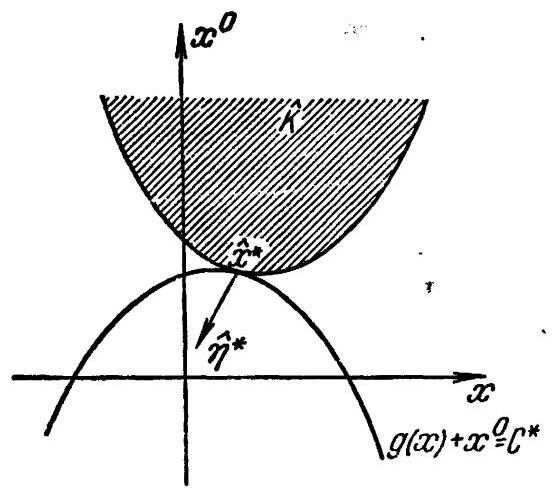
\includegraphics[max width=0.5\textwidth]{images/bo_d547k8bef24c73bgfcg0_193_840_423_552_490_0.jpg}
\end{center}
\hspace*{3em} 

Рис. 3.1. Оптимальное решение, лежа- щее в выпуклой области достижимости.

Если \(g\left( x\right)  > a\) , то

\[
\mathop{\lim }\limits_{{{x}^{0} \rightarrow  \infty }}\left\lbrack  {g\left( x\right)  + {x}^{0}}\right\rbrack   =  + \infty
\]

равномерно на \(\widehat{K}\) . Таким образом, существует число α>0, такое, что минимум \(\left\lbrack  {g\left( x\right)  + {x}^{0}}\right\rbrack\) на \(\widehat{K}\) до- стигается на компактном множе- CTBE \(\widehat{K} \cap  \left\lbrack  {{x}^{0} \leq  \alpha }\right\rbrack\) .

Предположим теперь, что \(g\left( x\right)\) выпуклая функция. Для любого действительного числа \({c}_{1}\) подмножество в R**, для которого

\[
g\left( x\right)  + {x}^{0} \leq  {c}_{1}
\]

является замкнутым и имеет непустую внутренность. Кроме того, это множество выпукло, поскольку из неравенства

\[
g\left( {x}_{1}\right)  + {x}_{1}^{0} \leq  {c}_{1}\;\mathrm{n}\;g\left( {x}_{2}\right)  + {x}_{2}^{0} \leq  {c}_{1}
\]

следует, что

\[
g\left( {\lambda {x}_{1} + \left( {1 - \lambda }\right) {x}_{2}}\right)  + \lambda {x}_{1}^{0} + \left( {1 - \lambda }\right) {x}_{2}^{0} \leq  {c}_{1}.
\]

Рассмотрим постоянное число с такое, что соответствующее ему множество пересекается с д’, и докажем, что это пересечение ограничено, и следовательно, компактно. Из этого утверждения будет непосредственно следовать существование оптимального управления.

Пусть π-гиперплоскость в R**, такая, что g (x)+x,-с для точек ( \({x}^{0},x\) ), лежащих ниже π; например, можно взять гипер- плоскость, опорную к этому выпуклому множеству. Мы покажем, что для точек ( \({x}^{0},x) \in  \widehat{K}\) с достаточно большими \(\left| x\right|\) выполняется неравенство \({x}^{0} > k\left| x\right|\) для заданного постоянного k > 0. Такие гочки \(\left( {{x}^{0},x}\right)\) из \(\widehat{K}\) должны лежать выше π,а значит,удовлетво- ряют неравенству g(x)+x0>c, Установив это, мы получим требуемую компактность, чем и завершим доказательство теоремы. Для точек ( \({x}^{0},x\) ) из \(\widehat{K}\) имеем

\[
\left| {x\left( T\right) }\right|  \leq  \left| {\Phi \left( T\right) {x}_{0}}\right|  + {\int }_{{t}_{0}}^{T}\left| {\Phi \left( T\right) {\Phi }^{-1}\left( s\right) B\left( s\right) }\right| \left| {u\left( s\right) }\right| {ds}.
\]

Если \(\left| {x\left( T\right) }\right|  \geq  2\left| {\Phi \left( T\right) {x}_{0}}\right|\) и

\[
\left| {\Phi \left( T\right) {\Phi }^{-1}\left( s\right) B\left( s\right) }\right|  \leq  M\;\left( {{t}_{0} \leq  s \leq  T}\right) ,
\]

ТО

\[
{\int }_{0}^{T}\left| {u\left( s\right) }\right| {ds} \geq  \frac{1}{2M}\left| {x\left( T\right) }\right|
\]

Пользуясь неравенством ШВарца, получаем

\[
{\int }_{{t}_{0}}^{T}\left| {u\left( s\right) }\right| {ds} \leq  {c}_{2}{\left\lbrack  {\int }_{{t}_{0}}^{T}\parallel u\left( s\right) {\parallel }^{2}ds\right\rbrack  }^{1/2}
\]

для постоянного \({c}_{2} > 0\) . Таким образом, если |x(T)|≥ \(\geq  2\left| {\Phi \left( T\right) {x}_{0}}\right|\) ,то

\[
{\left| x\left( T\right) \right| }^{2} \leq  4{M}^{2}{c}_{2}^{2}{\int }_{{t}_{0}}^{T}\parallel u\left( s\right) {\parallel }^{2}{ds} \leq  {c}_{3}{x}^{0}\left( T\right) .
\]

Следовательно,для достаточно больших \(\left| {x\left( T\right) }\right|\) имеем

\[
{x}^{0}\left( T\right)  \geq  k\left| {x\left( T\right) }\right|
\]

и точки \(\left( {{x}^{0}\left( T\right) ,x\left( T\right) }\right)\) из \(\widehat{K}\) лежат выше гиперплоскости π. Or- сюда следует, что замкнутое пересечение множеств

\[
g\left( x\right)  + {x}^{0} \leq  {c}_{1}\text{ и }\widehat{K}
\]

ограничено, а значит, компактно. Теорема существования доказана.

Поскольку действительная функция \(g\left( x\right)  + {x}^{0}\) монотонно убы- вает с убыванием х0, то оптимальное управление должно перево- дить систему в точку, лежащую на границе К в R\textasciicircum 1-1. На самом деле мы рассматриваем выпуклое множество к внутри линейного многообразия \(L\left( \widehat{K}\right)\) ,натянутого на это множество; оптимальное управление должно переводить систему в точку, лежащую на границе К относительно \(L\left( \widehat{K}\right)\) . Таким образом,наиболее важное значение имеют те управления, которые переводят систему в точки, лежащие на границе К относительно \(L\left( \widehat{K}\right)\) .

Определение. Рассмотрим управляемую систему в

(2)
\[
\dot{x} = A\left( t\right) x + B\left( t\right) u,
\]

с множеством достижимости \(\widehat{K} \subset  {R}^{n + 1}\) , соответствующим крите- рию качества C, и) Управление и (t) на интервале t, с < c < \(T\) , переводящее систему из точки (0, \({x}_{0}\) ) в некоторую граничную точку множества K (относительно линейного многообразия \(L\left( \widehat{K}\right)\) ), называется экстремальным управлением, а соответствующая ему траектория — экстремальной траекторией.

Следующая теорема, которая является выражением принципа максимума для рассматриваемой нами задачи, [утверждает, что выражение

\[
{\eta }_{0}\parallel u{\parallel }_{U}^{2} + \eta \left( t\right) B\left( t\right) u
\]

достигает максимального значения при \(u = \bar{u}\left( t\right)\) ,где \(\bar{u}\left( t\right)\) — неко- торое экстремальное управление. Здесь \(\widehat{\eta }\left( t\right)  = \left( {{\eta }_{0},\eta \left( t\right) }\right)\) представ- ляет собой \(\left( {n + 1}\right)\) -мерный вектор-строку с постоянной компонен- той \({\eta }_{0} < 0\) . Поскольку

\[
\parallel u{\parallel }_{U}^{2} - \frac{\eta }{\left| {\eta }_{0}\right| }{Bu} = {\left\lVert \begin{array}{c} u - \frac{{U}^{-1}{B}^{\prime }{\eta }^{\prime }}{2\left| {\eta }_{0}\right| } \end{array} \right\rVert}_{U}^{2} - {\left\lVert \begin{array}{c} \frac{{U}^{-1}{B}^{\prime }{\eta }^{\prime }}{2\left| {\eta }_{0}\right| } \end{array} \right\rVert}_{U}^{2},
\]

то макснмум выражения \({\eta }_{0}\parallel u{\parallel }_{U}^{2} + {\eta Bu}\) достигается лншь при

\[
u\left( t\right)  =  - \frac{U - \left( {t}^{1}\right) {B}^{\prime }\left( t\right) {\eta }^{\prime }\left( t\right) }{2\left| {\eta }_{0}\right| }.
\]

Теорема 3. Рассмотрим управляемую систему в R":

(
\[
\mathcal{L}
\]
 )
\[
\dot{x} = A\left( t\right) x + B\left( t\right) u.
\]

Управление и (t) с соответствующим решением х(t) (t, c ≤ t ≤ T), является экстремальным в том и только том случае, когда су- ществует (n+1)-мерный вектор \(\widehat{\eta }\left( t\right)  = \left( {{\eta }_{0},\eta \left( t\right) }\right) ,y\partial\) овлетворяющий уравнению

\[
\dot{\eta } =  - 2{\eta }_{0}{\bar{x}}^{\prime }\left( t\right) W\left( t\right)  - {\eta A}\left( t\right) \text{ , }\varepsilon \partial e\text{ norm and }{\eta }_{0} < 0\text{ , }
\]

maxoǔ, umo

\[
{\eta }_{0}\parallel \bar{u}\left( t\right) {\parallel }_{U}^{2} + \eta \left( t\right) B\left( t\right) \bar{u}\left( t\right)  = \mathop{\max }\limits_{{u \in  {R}^{m}}}\left\{  {{\eta }_{0}\parallel u{\parallel }_{U}^{2} + \eta \left( t\right) B\left( t\right) u}\right\}
\]

unu

\[
\bar{u}\left( t\right)  =  - \frac{1}{2{\eta }_{0}}{U}^{-1}\left( t\right) {B}^{\prime }\left( t\right) {\eta }^{\prime }\left( t\right) \;\text{ no }u\text{ mu }{\theta c} + o\partial y.
\]

Доказательство. Пусть хеметием соответствующее управлению

\[
\bar{u}\left( t\right)  =  - \frac{1}{2{\eta }_{0}}{U}^{-1}\left( t\right) {B}^{\prime }\left( t\right) {\eta }^{\prime }\left( t\right) ,
\]

где \(\widehat{\eta }\left( t\right)  = \left( {{\eta }_{0},\eta \left( t\right) }\right)\) - вектор, Удовлетворяющий дифференциаль ному уравнению

\[
\dot{\eta } =  - 2{\eta }_{0}{\bar{x}}^{\prime }\left( t\right) W\left( t\right)  - {\eta A}\left( t\right) ,
\]

а постоянная \({\eta }_{0} < 0\) . Поскольку в предположениях теоремы участ- вует, по существу, лишь отношение η/η, то для удобства изло- жения можно выбрать \({\eta }_{0} =  - 1/2\) . Мы докажем,что

\[
\widehat{\eta }\left( T\right) \widehat{x}\left( T\right)  > \widehat{\eta }\left( T\right) \widehat{\omega }
\]

для всех точек \(\widehat{\omega } = \left( {{\omega }^{0},\omega }\right)\) из \(\widehat{K}\) , OTЛN4Hыx OT \(\widehat{x}\left( T\right)  = \left( {\overrightarrow{{x}^{0}}\left( T\right) }\right.\) , \(x\left( T\right) )\) . Из этого неравенства мы заключим,что \(\widehat{x}\left( T\right)\) лежит на границе (относительной) множества К. Здесь м (н сы общее ре- шение, соответствующее управлению и (t), и определенное равен- CTBAMH

\[
{\omega }^{0}\left( t\right)  = {\int }_{{t}_{0}}^{t}\left\lbrack  {\parallel \omega \left( s\right) {\parallel }_{W}^{2} + \parallel u\left( s\right) {\parallel }_{U}^{2}}\right\rbrack  {ds},
\]

\[
\omega \left( t\right)  = \Phi \left( t\right) {x}_{0} + {\int }_{{t}_{0}}^{t}\Phi \left( t\right) {\Phi }^{-1}\left( s\right) B\left( s\right) u\left( s\right) {ds}.
\]

MMeem

\[
\frac{d}{dt}\left( {\widehat{\eta }\left( t\right) \widehat{\omega }\left( t\right) }\right)  =  - \frac{1}{2}{\dot{\omega }}^{0} + \dot{\eta }\omega  + \eta \dot{\omega } =
\]

\[
=  - \frac{1}{2}\left\lbrack  {\parallel \omega {\parallel }_{W}^{2} + \parallel u{\parallel }_{U}^{2}}\right\rbrack   + {\bar{x}}^{\prime }{W\omega } - {\eta A\omega } + {\eta A\omega } + {\eta Bu}.
\]

Интегрированне от \({t}_{0}\) до é дает

\[
- \frac{1}{2}{\omega }^{0}\left( t\right)  + \eta \left( t\right) \omega \left( t\right)  - \eta \left( {t}_{0}\right) {x}_{0} =
\]

\[
\backslash   = \mathop{\int }\limits_{{t}_{0}}^{t}\left\{  {-\frac{1}{2}\left\lbrack  {{\left\lVert \begin{array}{c} \omega \end{array} \right\rVert}_{W}^{2} + {\left\lVert \begin{array}{c} u \end{array} \right\rVert}_{U}^{2}}\right\rbrack   + \left\lbrack  {{\omega }^{\prime }W\left( s\right) \bar{x}\left( s\right)  + {\eta B}\left( s\right) u\left( s\right) }\right\rbrack  }\right\}  {ds}.
\]

Для случая, когда и (s) \(= \bar{u}\left( s\right)  = {U}^{-1}\left( s\right) {B}^{\prime }\left( s\right) {\eta }^{\prime }\left( s\right)\) и \(\widehat{\omega }\left( s\right)  = \widehat{x}\left( s\right)\) , это выражение имеет более простой вид:

\[
- \frac{1}{2}{\bar{x}}^{0}\left( t\right)  + \eta \left( t\right) \bar{x}\left( t\right)  - \eta \left( {t}_{0}\right) {x}_{0} = \frac{1}{2}{\int }_{{t}_{0}}^{t}\left\lbrack  {\parallel \bar{x}\left( s\right) {\parallel }_{W}^{2} + {\left\lVert \begin{array}{c} {\eta }^{\prime }\left( s\right) \end{array} \right\rVert}_{B{U}^{-1}{B}^{\prime }}^{2}}\right\rbrack  {ds}.
\]

Очевидно, что выражение \(- \frac{1}{2}\parallel u{\parallel }_{U}^{2} + {\eta Bu}\) достигает максимума лишь при

\[
u = {U}^{-1}\left( s\right) {B}^{\prime }\left( s\right) {\eta }^{\prime }\left( s\right) .
\]

3Hault, \(\operatorname{ec\text{ л }\text{ н }}u\left( s\right)  \neq  \bar{u}\left( s\right)\) , to

\[
- \frac{1}{2}\parallel u\left( s\right) {\parallel }_{U}^{2} + {\eta B}\left( s\right) u\left( s\right)  < \frac{1}{2}{\left\lVert \begin{array}{c} {\eta }^{\prime }\left( s\right) \end{array} \right\rVert}_{B{U}^{-1}{B}^{\prime }}^{2}.
\]

Далее,из неравенства \(\parallel \bar{x}\left( s\right)  - \omega \left( s\right) {\parallel }_{W}^{2} \geq  0\) следуег,что

\[
\frac{1}{2}\parallel \bar{x}\left( s\right) {\parallel }_{W}^{2} \geq  {\omega }^{\prime }W\left( s\right) \bar{x} - \frac{1}{2}\parallel \omega \left( s\right) {\parallel }_{W}^{2}.
\]

Таким образом, если почти всюду на \(0 \leq  t \leq  T\) не выполняется равенство \(u\left( t\right)  = \bar{u}\left( t\right)\) , то

\[
- \frac{1}{2}{\bar{x}}^{0}\left( t\right)  + \eta \left( t\right) \bar{x}\left( t\right)  - \eta \left( {t}_{0}\right) {x}_{0} >  - \frac{1}{2}{\omega }^{0}\left( t\right)  + \eta \left( t\right) \omega \left( t\right)  - \eta \left( {t}_{0}\right) {x}_{0}.
\]

Cледовательно,

\[
\widehat{\eta }\left( T\right) \widehat{x}\left( T\right)  > \widehat{\eta }\left( T\right) \widehat{\omega }\left( T\right)
\]

для всех @ (T) ≠ (T) из \(\widehat{K}\) . Но это неравенство означает, что существует гиперплоскость, опорная к К в точке х (т) с внеш- ней нормалью \(\widehat{\eta }\left( T\right)\) . Поскольку η0 с 0, то опорная гиперпло- скость не может пересекаться с множеством \(\widehat{K}\) по его внутрен- ним точкам, а может пересекать к лишь по граничным точкам (относительным). Таким образом, управление и (и) и решение \(\bar{x}\left( t\right)\) экстремальны.

Обратно, предположим, что управление и (и) порождает траек- торию \(\widehat{x}\left( t\right)  = \left( {{\bar{x}}^{0}\left( t\right) ,\bar{x}\left( t\right) }\right)\) ,ведущую в точку ёх (T) едк. Пусть \(\widehat{\eta }\left( T\right)  = \left( {-\frac{1}{2},\overline{\eta }\left( T\right) }\right)\) -внешняя нормаль к \(\widehat{K}\) в точке \(\widehat{x}\left( T\right)\) ; опре- делим \(\overline{\eta }\left( t\right)\) как решение сопряженной системы

\[
\dot{\eta } = {\bar{x}}^{\prime }\left( t\right) W\left( t\right)  - {\eta A}\left( t\right) .
\]

Мы должны показать, что \(\bar{u}\left( t\right)  = {U}^{-1}\left( t\right) {B}^{\prime }\left( t\right) \overline{\eta }\left( t\right)\) почти всюду на интервале б, с < t < T. Предположим, что ш (t) не удовлетворяет принципу максимума на некотором подмножестве Δ - интервале ненулевой длины [можно считать подмножество ∆ компактным, a управление \(\bar{u}\left( t\right)\) orpaниченным на \(\Delta \rbrack\) ,где - \(\frac{1}{2}\parallel \bar{u}{\parallel }_{U}^{2} + \; + \overline{\eta }\left( t\right) B\left( t\right) \bar{u}\left( t\right)  + \delta  \leq  \mathop{\max }\limits_{u}\left\lbrack  {-\frac{1}{2}\parallel u{\parallel }_{v}^{2} + \overline{\eta }\left( t\right) B\left( t\right) u}\right\rbrack\) для некото- poro \(\delta  > 0\) . Для каждого малого в > 0 определим возмущенное управление

\({u}_{\varepsilon }\left( t\right)  = \left\{  \begin{array}{cc} {U}^{-1}\left( t\right) {B}^{\prime }\left( t\right) \overline{\eta }\left( t\right) & \text{ на подмножестве }\Delta \text{ меры }\varepsilon \text{ I } \\  \bar{u}\left( t\right) & \text{ на остальной части }{t}_{0} \leq  t \leq  T. \end{array}\right.\)

Пусть соответствующим решением будет х, что

\(\left| {{\widehat{x}}_{n}\left( t\right)  - \widehat{x}\left( t\right) }\right|  \leq  {c}_{1}\varepsilon\) для некоторой постоянной \({c}_{1}\) .

Как и выше, получим

\[
\widehat{\eta }\left( T\right) \widehat{x}\left( T\right)  - \widehat{\eta }\left( T\right) {\widehat{x}}_{\varepsilon }\left( T\right)  \leq  {\int }_{{t}_{0}}^{T}\frac{1}{2}{\left\lVert \begin{array}{c} \overrightarrow{x} - {x}_{\varepsilon } \end{array} \right\rVert}_{W}^{2}{dt} - {\int }_{{\Delta }_{\varepsilon }}{\delta dt} \leq  {a}_{2}{\varepsilon }^{2} - {\delta \varepsilon }
\]

аля постоянной сдкнм образом,для достаточно малых в \(> 0\)

\[
\widehat{\eta }\left( T\right) {\widehat{x}}_{s}\left( T\right)  > \widehat{\eta }\left( T\right) \widehat{x}\left( T\right)
\]

что невозможно, если д/(Т) есть внешняя нормаль к К в точке \(x\left( T\right)\) . Следовательно, \(\bar{u}\left( t\right)\) должно удовлетворять принципу мак- симума. Теорема доказана.

В теореме 3 утверждается, что управление и (и) является -эк- стремальным тогда и только тогда, когда оно максимально (в смысле главы 1). Поэтому мы в дальнейшем не будем пользоваться тер- мином «максимальное управление».

Cледствие. Рассмотрим управляемую систему в R":

(
\[
\mathcal{L}
\]
 )
\[
\dot{x} = A\left( t\right) x + B\left( t\right) u
\]

с крциерцем качеспва

\[
C\left( u\right)  = g\left( {x\left( T\right) }\right)  + {\int }_{{t}_{0}}^{T}\left\lbrack  {\parallel x\left( s\right) {\parallel }_{W}^{2} + \parallel u\left( s\right) {\parallel }_{U}^{2}}\right\rbrack  {ds}.
\]

Пусть и «(t) — оптимальное управление с соответствующим реше нием к’*(t) на интервале t, ±<t<T. Тогда и*(t) является экстре- мальным управлением, т. е. существует n-мерный вектор η(t), удовлетворяющий уравнению

\[
\dot{\eta } = {x}^{*\prime }\left( t\right) W\left( t\right)  - {\eta A}\left( t\right) ,
\]

maxoǔ, umo

\[
{u}^{ * }\left( t\right)  = {U}^{-1}\left( t\right) {B}^{r}\left( t\right) {\eta }^{\prime }\left( t\right) \;\text{ noumu acto }\partial y.
\]

Условия нормальности, которые обеспечивают единственность экстремального управления, переводящего систему из точки (0, x, в граничную точку множества K, для наших систем, линейных, с интегральным квадратическим критерием качества, выполняются автоматически. Таким образом, максимальное условие теоремы 3 является как необходимым, так -и достаточным условием опти- мальности данного управления. В теореме 4 мы докажем эту единственность, а в теореме 5 и в примерах следующего раздела будем применять доказанные свойства к построению оптимальных управлений.

Теорема 4. Рассмотрим управляемую систему в R":

(L)
\[
\dot{x} = A\left( t\right) x + B\left( t\right) u,
\]

с множеством достижимости К с е пипыт соответствующим крите- рию качества Co (и). Пусть и и (1) и и си (1) — экстремальные управле- ния с соответствующими решениями. к, (1) и х, (1) в Рич на ин- тервале t, в с л сл сли

\[
{\widehat{x}}_{1}\left( T\right)  = {\widehat{x}}_{2}\left( T\right) ,\;\text{ mo }\;{u}_{1}\left( t\right)  = {u}_{2}\left( t\right) \;\text{ no }u\text{ au }\theta \text{ co }\partial y.
\]

Доказательство. Пусть д ( \(T\) ) есть внеш- няя нормаль к \(\widehat{K}\) в точке \(\widehat{{x}_{1}}\left( T\right)  = {\widehat{x}}_{1}\left( T\right)\) и пусть η(t) — соответ- ствующее решение уравнения

\[
\dot{\eta } = {x}_{1}^{\prime }\left( t\right) W\left( t\right)  - {\eta A}\left( t\right)
\]

Тогда, как показано в теореме 3,

\[
{u}_{1}\left( t\right)  = {u}_{2}\left( t\right)  = {U}^{-1}\left( t\right) {B}^{\prime }\left( t\right) {\eta }^{\prime }\left( t\right) \text{ почти всюду. }
\]

Действительно, в противном случае число у (т) к \(= \widehat{\eta }\left( T\right) {\widehat{x}}_{2}\left( T\right)\) было бы меньше,чем \(\widehat{\eta }\left( T\right) \widehat{\omega }\) для некоторого \(\widehat{\omega } \in  \widehat{K}\) . Теорема доказана.

Teopeмa 5. Рассмотрим управляемую систему в R":

\[
\left( \mathcal{L}\right)
\]

\[
\dot{x} = A\left( t\right) x + B\left( t\right) u,
\]

с крциерцем качесмеа

\[
C\left( u\right)  = g\left( {x\left( T\right) }\right)  + {\int }_{{t}_{0}}^{T}\left\lbrack  {\parallel x{\parallel }_{W}^{2} + \parallel u{\parallel }_{U}^{2}}\right\rbrack  {ds} = g\left( {x\left( T\right) }\right)  + {C}_{0}\left( u\right) ,
\]

где g(x)—некоторая выпуклая функция из С'1. Тогда существует единственная гиперповерхность \({S}_{m}\) из семейства

\[
{S}_{c} : g\left( x\right)  + {x}^{0} = c,
\]

касательная к л; следовательно, т есть оптимальное значение критерия качества. Кроме того, существует единственное экстре- мальное управление, а именно, оптимальное управление и*(н), с помощью которого достигается та единственная точка, где Sm касается \(\widehat{K}\) .

Далее, система дифференциальных уравнений

\[
\dot{x}\;A\left( t\right) x + B\left( t\right) {U}^{-1}\left( t\right) {B}^{\prime }\left( t\right) {\eta }^{\prime },
\]

\[
\dot{\eta } = {x}^{\prime }W\left( t\right)  - {\eta A}\left( t\right)
\]

имеем еòuhспвенное реиение, убовлемворяющее эранииным условиям

\[
x\left( {t}_{0}\right)  = {x}_{0}\;u\;\eta \left( T\right)  =  - \frac{1}{2}\operatorname{grad}g\left( {x\left( T\right) }\right) ,
\]

а именно, оптимальное решение х*(t) и т*(t) такое, что управ- ление

\[
{u}^{ * }\left( t\right)  = {U}^{-1}\left( t\right) {B}^{\prime }\left( t\right) {\eta }^{*\prime }\left( t\right)
\]

является оптимальным на интервале б, е х с х и ох. чы

Доказательство. Прежде всего мы покажем, что имеется единственное постоянное \(m\) такое,что \({S}_{m}\) касается \(\widehat{K}\) [множества достижимости, соответствующего критерию \({C}_{0}\left( u\right)\) ],т. е. выпуклое множество \(g\left( x\right)  + {x}^{0} \leq  m\) пересекается с \(\widehat{K}\) ,но отделяется от его относительной внутренности общей опорной гиперплоскостью π*, касательной к \$„ Огсюда будет следовать, что тесть минималь- ное значение критерия. По теореме 2 пересечение множества К с совокупностью точек, удовлетворяющих неравенству \(g\left( x\right)  + {x}^{0} \leq  c\) , является компактным множеством для всех достаточно больших с. Поэтому мы определим m как нижнюю грань всех таких чисел c, для которых рассматриваемое пересечение непусто. Для \(c > m\) гиперповерхность \({S}_{c}\) пересекается с Ём по относительно внутрен- ним точкам множества K, а для \(c < m\) гиперповерхность \({S}_{c}\) вовсе не пересекает К. Таким образом, только при c=m ruпер- поверхность \({S}_{c}\) может лишь касаться к.

Пусть \(P\) -точка, \(\Pi\) ринадлежащая \(\widehat{K} \cap  {S}_{m}\) и пусть \({\pi }^{ * }\) - каса- тельная гиперплоскость к \({S}_{m}\) в точке \(P\) . Тогда я* не будет раз- делять \(\widehat{K}\) и \({S}_{m}\) лишь в том случае, если т’ пересекает множе- ство К по его внутренним точкам. Предположим, однако, что имеется (относительно) открытое множество N внутренних точек в К, лежащее ниже гиперплоскости π*. Тогда и весь конус с ос- нованием N и вершиной P лежит ниже π*, и внутри К. Однако Sm касается \({\pi }^{ * }\) в точке \(P\) ,так что \({S}_{m}\) будет пересекать \(\widehat{K}\) по внутрен- ним точкам. Но это невозможно по определению m. Следовательно, гиперплоскость \({\pi }^{ * }\) paзделяет \(\widehat{K}\) и \({S}_{m}\) .

Предположим теперь, что множество К̂ N S… содержит две различные точки \({P}_{1}\) и \({P}_{2}\) . Тогда и весь отрезок, соединяющий их, лежит в К/ М, в значит, он входит в относительную границу К. Рассмотрим экстремальные управления \({u}_{1}\left( t\right)\) и \({u}_{2}\left( t\right)\) с решениями \({\widehat{x}}_{1}\left( t\right)\) и \({\widehat{x}}_{2}\left( t\right)\) ,приводящими в точки \({P}_{1}\) и \({P}_{2}\) соответственно. Заме- тим, что управления \({u}_{1}\left( t\right)\) и \({u}_{2}\left( t\right)\) должны отличаться друг от друга на некотором множестве ненулевой меры из \({t}_{0} \leq  t \leq  T\) .

Рассмотрим управление \(\frac{1}{2}\left\lbrack  {{u}_{1}\left( t\right)  + {u}_{2}\left( t\right) }\right\rbrack\) с соответствующим решением

3 rech

\[
\widehat{x}\left( t\right)  = \left( {{x}^{0}\left( t\right) ,x\left( t\right) }\right) .
\]

\[
x\left( T\right)  = \frac{1}{2}\left\lbrack  {{x}_{1}\left( T\right)  + {x}_{2}\left( T\right) }\right\rbrack  .
\]

Oднако мы покажем, что

\[
{x}^{0}\left( T\right)  < \frac{1}{2}\left\lbrack  {{x}_{1}^{0}\left( T\right)  + {x}_{2}^{0}\left( T\right) }\right\rbrack  .
\]

Nmeem

\[
{x}^{0}\left( T\right)  = {\int }_{{t}_{0}}^{T}\left\lbrack  {{\left\lVert \begin{array}{c} \frac{{x}_{1}\left( s\right)  + {x}_{2}\left( s\right) }{2} \end{array} \right\rVert}_{W}^{2} + {\left\lVert \begin{array}{c} \frac{{u}_{1}\left( s\right)  + {u}_{2}\left( s\right) }{2} \end{array} \right\rVert}_{U}^{2}}\right\rbrack  {ds} =
\]

\[
= {\int }_{{t}_{0}}^{T}\left\{  {\frac{1}{4}{\left\lVert \begin{array}{c} {x}_{1} \end{array} \right\rVert}_{W}^{2} + \frac{1}{2}{x}_{1}^{\prime }W\left( s\right) {x}_{2} + \frac{1}{4}{\left\lVert \begin{array}{c} {x}_{2} \end{array} \right\rVert}_{W}^{2} + \frac{1}{4}{\left\lVert \begin{array}{c} {u}_{1} \end{array} \right\rVert}_{U}^{2} + }\right.
\]

\[
\left. {+\frac{1}{2}{u}_{1}^{\prime }U\left( s\right) {u}_{2} + \frac{1}{4}{\left\lVert \begin{array}{c} {u}_{2} \end{array} \right\rVert}_{U}^{2}}\right\}  {ds}.
\]

Используем очевидные неравенства

и

\[
2{x}_{1}^{\prime }\left( s\right) {W}^{\prime }\left( s\right) {x}_{2}\left( s\right)  \leq  {\left\lVert \begin{array}{c} {x}_{1}\left( s\right) \end{array} \right\rVert}_{W}^{2} + {\left\lVert \begin{array}{c} {x}_{2} \end{array} \right\rVert}_{W}^{2}
\]

\[
2{u}_{1}^{\prime }\left( s\right) U\left( s\right) {u}_{2}\left( s\right)  < {\left\lVert \begin{array}{c} {u}_{1}\left( s\right) \end{array} \right\rVert}_{U}^{2} + {\left\lVert \begin{array}{c} {u}_{2} \end{array} \right\rVert}_{U}^{2},
\]

справедливые всюду, где \({u}_{1}\left( s\right)  \neq  {u}_{2}\left( s\right)\) . Тогда

\[
{x}^{0}\left( T\right)  < \frac{1}{2}{\int }_{{t}_{0}}^{T}\left\lbrack  {{\left\lVert \begin{array}{c} {x}_{1} \end{array} \right\rVert}_{W}^{2} + {\left\lVert \begin{array}{c} {u}_{1} \end{array} \right\rVert}_{U}^{2}}\right\rbrack  {ds} + \frac{1}{2}{\int }_{{t}_{0}}^{T}\left\lbrack  {{\left\lVert \begin{array}{c} {x}_{2} \end{array} \right\rVert}_{W}^{2} + {\left\lVert \begin{array}{c} {u}_{2} \end{array} \right\rVert}_{U}^{2}}\right\rbrack  {ds},
\]

ТАК ЧТО

\[
{x}^{0}\left( T\right)  < \frac{1}{2}\left\lbrack  {{x}_{1}^{0}\left( T\right)  + {x}_{2}^{0}\left( T\right) }\right\rbrack  ,\;\text{ Kak и утверждалось выше. }
\]

Полупрямая \({x}^{0} > {x}^{0}\left( T\right) ,x = x\left( T\right)\) лежит внутри К, откуда следует, что и середина отрезка, соединяющего точки \({P}_{1}\) и \({P}_{2}\) ,лежит внутри К. Но 2 ( \({P}_{1} + {P}_{2}\) ) находится на относительной границе множества K. Это противоречие доказывает, что множество R ( \({S}_{m}\) состоит в точности из одной точки P.

По теореме 4 существует единственное экстремальное управле- ние, переводящее систему из точки (0, x) в точку \(P \in  \widehat{K}\) , значит, это и есть оптимальное управление и « (t). Следовательно, точка \(P = \left( {{x}^{0 * }\left( T\right) ,{x}^{ * }\left( T\right) }\right)\) должна быть достигнута при движении по оптимальной траектории \({x}^{ * }\left( t\right)\) .

Bektop \({\widehat{\eta }}^{ * }\left( T\right)  = \left( {-\frac{1}{2},{\eta }^{ * }\left( T\right) }\right)\) является нормальным к \({S}_{m}\) в точке \(P = {\widehat{x}}^{ * }\left( T\right)\) ,где \({\eta }^{ * }\left( T\right)  =  - \frac{1}{2}\operatorname{grad}g\left( P\right)\) . По теореме 3 функции х*(t) и η*(t) удовлетворяют уравнениям

\[
\dot{x} = A\left( t\right) x + B\left( t\right) {U}^{-1}\left( t\right) {B}^{\prime }\left( t\right) {\eta }^{\prime },
\]

\[
\dot{\eta } = {x}^{\prime }W\left( t\right)  - {\eta A}\left( t\right)
\]

сграничными условиями

\[
{x}^{ * }\left( {t}_{0}\right)  = {x}_{0},\;{\eta }^{ * }\left( T\right)  =  - \frac{1}{2}\operatorname{grad}g\left( {{x}^{ * }\left( T\right) }\right) .
\]

Пусть теперь \(x\left( t\right) ,\eta \left( t\right)\) —любое решение этой совместной системы дифференциальных уравнений с заданными граничными условиями. Тогда \(\widehat{x}\left( t\right)  = \left( {{x}^{0}\left( t\right) ,x\left( t\right) }\right)\) есть решение, определяемое экстремаль- ным управлением \(u\left( t\right)  = {U}^{-1}\left( t\right) {B}^{\prime }\left( t\right) {\eta }^{\prime }\left( t\right)\) . Более того,

\[
\widehat{\eta }\left( T\right) \widehat{x}\left( T\right)  =  - \frac{1}{2}{x}^{0}\left( T\right)  + \eta \left( T\right) x\left( T\right)  > \widehat{\eta }\left( T\right) \widehat{\omega }
\]

для всех @ ≠ \(\widehat{x}\left( T\right)\) из \(\widehat{K}\) . Таким образом, вектор \(\widehat{\eta }\left( T\right)  = \left( {-\frac{1}{2},\eta \left( T\right) }\right)\) является внешней нормалью к опорной гиперплоскости π множе- ства К в точке X(T). Кроме того, \(\widehat{\eta }\left( T\right)\) есть внутренняя нормаль \(\mathrm{K}\) гиперповерхности \({S}_{c}\) в \(\widehat{x}\left( T\right)\) ,поскольку \(\eta \left( T\right)  =  - \frac{1}{2}\operatorname{grad}g\left( {x\left( T\right) }\right)\) . Таким образом, гиперповерхность \({S}_{c}\) касается множества К в точке х (т) и я есть их общая опорная гиперплоскость. Но тогда \({S}_{c} = {\mathcal{S}}_{m}\) и \(\widehat{x}\left( T\right)  = {\widehat{x}}^{ * }\left( T\right)\) . B силу единственности экстре- мального управления, переводящего систему из состояния (0, \%) в состояние \({x}^{ * }\left( T\right)\) ,находим,что \(u\left( t\right)  = {u}^{ * }\left( t\right)\) почти всюду,и зна- чит, \(x\left( t\right)  = {x}^{ * }\left( t\right)\) на интервале \({t}_{0} \leq  t \leq  T\) . Итак, окончательно, \(\eta \left( t\right)\) есть единственное решение уравнения

\[
\dot{\eta } = {x}^{*\prime }\left( t\right) W\left( t\right)  - {\eta A}\left( t\right)
\]

C

\[
\eta \left( T\right)  =  - \frac{1}{2}\operatorname{grad}g\left( {{x}^{ * }\left( T\right) }\right)
\]

H, 3Ha4HT,

\[
\eta \left( t\right)  = {\eta }^{ * }\left( t\right) \;\text{ На }\;{t}_{0} \leq  t \leq  T.
\]

Теорема доказана.

Если нам нужно перевести систему из заданной начальной точки \({x}_{0} \in  {R}^{n}\) в некоторое желаемое состояние, то естественно потребовать, чтобы система

(L)
\[
\dot{x} = A\left( t\right) x + B\left( t\right) u
\]

обладала свойством управляемости. Система 𝒳 будет вполне управляемой, если для любой пары точек \({x}_{0},{x}_{1} \in  {R}^{n}\) существует ограниченное измеримое управление \(u\left( t\right)\) ,переводящее систему из точки \(x\left( {t}_{0}\right)  = {x}_{0}\) в точку \(x\left( T\right)  = {x}_{1}\) . Случай полной управляемости легче поддается геометрическому анализу, так как тогда множе- ство достижимости \(\widehat{K}\) имеет непустую внутренность в \({R}^{n + 1}\) ,и сле- довательно, граница множества К относительно \(L\left( \widehat{K}\right)  = {R}^{n + 1}\) co- впадает с обычной границей.

Теорема 6. Рассмотрим управляемую систему в R":

\[
\left( \mathcal{L}\right)
\]

\[
\dot{x} = A\left( t\right) x + B\left( t\right) u,
\]

с множеством достижимости КС Рич, соответствующим крите- рию качества Co (и). Система 20 обладает свойством управляемо- сти на интервале б, с 4 с тогда и только тогда, когда мно- жество К имеет непустую внутренность в R"+1, а это будет в том, и только в том случае, если матрица

\[
M\left( T\right)  = {\int }_{{t}_{0}}^{T}{\Phi }^{-1}\left( t\right) B\left( t\right) {B}^{\prime }\left( t\right) {\left( {\Phi }^{-1}\left( t\right) \right) }^{\prime }{dt}
\]

heebiposicdeha.

Доказательство. Ортогональная проекция множества К на подпространство \({x}^{0} = 0\) представляет собой совокупность всех концов траекторий в \({R}^{n}\) :

\[
x\left( T\right)  = \Phi \left( T\right) {x}_{0} + \Phi \left( T\right) {\int }_{{t}_{0}}^{T}{\Phi }^{-1}\left( t\right) B\left( t\right) u\left( t\right) {dt}.
\]

Если система У обладает свойством управляемости, то множество всех концов траекторий \(\{ x\left( T\right) \}\) совпадает со всем пространством \({R}^{n}\) , и значит, множество К имеет непустую внутренность. С другой стороны, если К имеет непустую внутренность, то в силу леммы к теореме 1 \{x(T)\}=R". Но это означает, что множество всех точек вида

\[
{x}_{1} = {\int }_{{t}_{0}}^{T}\Phi \left( T\right) {\Phi }^{-1}\left( t\right) B\left( t\right) u\left( t\right) {dt}
\]

заполняет все пространство. Значит, совокупность всех концов траекторий, начинающихся в произвольной фиксированной точке пространства \({R}^{n}\) , совпадает со всем \({R}^{n}\) . [3десь и (t) пробегает пространство \({L}_{2}\) , oднако,так как измеримые ограниченные функ- ции плотны в \({L}_{2}\) ,можно считать,что все управления и (t) orpa- ничены]. Таким образом, в этом случае система 오 обладает свойством управляемости.

Рассмотрим теперь \(\left( {n \times  n}\right)\) -матрицу \(M\left( T\right)\) . Поскольку

\[
{M}^{\prime }\left( T\right)  = {\int }_{{t}_{0}}^{T}{\left\lbrack  {\Phi }^{-1}\left( t\right) B\left( t\right) {B}^{\prime }\left( t\right) {\left( {\Phi }^{-1}\left( t\right) \right) }^{\prime }\right\rbrack  }^{\prime }{dt} = M\left( T\right) ,
\]

a takke

\[
{\zeta }^{\prime }M\left( T\right) \zeta  = {\int }_{{t}_{0}}^{T}{\left( {B}^{\prime }{\left( {\Phi }^{-1}\right) }^{\prime }\zeta \right) }^{\prime }\left( {{B}^{\prime }{\left( {\Phi }^{-1}\right) }^{\prime }\zeta }\right) {dt} \geq  0
\]

для любого n-мерного вектора ζ, то матрица M (T) симметриче- ская и неотрицательно определенная.

Предположим, что матрица М(Т) невырождена, и докажем, что система 8 вполне управляема. Для заданных точек и, и их и определим управление

\[
u\left( t\right)  = {B}^{\prime }\left( t\right) {\left( {\Phi }^{-1}\left( t\right) \right) }^{\prime }\xi ,
\]

где постоянный вектор \(\xi\) определяется формулой

B этом случае

\[
\xi  = {M}^{-1}\left( T\right) \left\lbrack  {{\Phi }^{-1}\left( T\right) {x}_{1} - {x}_{0}}\right\rbrack  .
\]

\[
{x}_{1} = \Phi \left( T\right) {x}_{0} + \Phi \left( T\right) M\left( T\right) \xi
\]

или

\[
{x}_{1} = \Phi \left( T\right) {x}_{0} + \Phi \left( T\right) {\int }_{{t}_{0}}^{T}{\Phi }^{-1}\left( t\right) B\left( t\right) u\left( t\right) {dt},
\]

что и требуется.

C другой стороны, предположим, что система 𝒳 обладает свойством управляемости. Если матрица М(Т) вырождена, то существует постоянный вектор \(\xi  \neq  0\) ,такой,что

\[
{\zeta }^{\prime }M\left( T\right) \zeta  = {\int }_{{t}_{0}}^{T}{\left\lVert \begin{array}{c} {B}^{\prime }\left( t\right) {\left( {\Phi }^{-1}\left( t\right) \right) }^{\prime }\zeta \end{array} \right\rVert}^{2}{dt} = 0.
\]

Но это означает, что ву (t) \({\left( {\Phi }^{-1}\left( t\right) \right) }^{\prime }\zeta  \equiv  0\) на интервале \({t}_{0} \leq  t \leq  T\) . Поскольку система 8 обладает свойством управляемости, то ко- нечная точка \(\Phi \left( T\right) \zeta\) может быть достигнута системой, исходя из начала координат, с помощью управления и (t) и, значит,

\[
\zeta  = {\int }_{{t}_{0}}^{T}{\Phi }^{-1}\left( t\right) B\left( t\right) u\left( t\right) {dt}
\]

Но rotaa

\[
0 < {\zeta }^{\prime }\zeta  = {\int }_{{t}_{0}}^{T}{\zeta }^{\prime }{\Phi }^{-1}\left( t\right) B\left( t\right) u\left( t\right) {dt} = {\int }_{{t}_{0}}^{T}{\left( {B}^{\prime }\left( t\right) {\left( {\Phi }^{-1}\left( t\right) \right) }^{\prime }\zeta \right) }^{\prime }u\left( t\right) {dt} = 0.
\]

Это противоречие указывает на то, что М(Т) —невырожденная матрица. Теорема доказана.

B частности, если матрица Ф-1() В (н) В/(1) (Ф-1(+))′невырож- дена хотя бы в один из моментов t, то матрица М(Т) будет не- вырожденной матрицей, и система 8 будет обладать свойством управляемости на интервале t, с хстема 𝒳 одиден Свойством

\section*{3.3. Иллюстрирующие примеры и специальные задачи}

В этом разделе мы рассмотрим вопросы синтеза управления с обратной связью для различных оптимальных управляемых систем, опираясь на теорию, изложенную в предыдущем разделе. Вначале будут рассматриваться задачи, в которых целевое множе- ство не задано заранее, затем задачи с заданным целевым множе- ством и, наконец, задачи с неограниченным временем управления.

Критерийкачества

\[
C\left( u\right)  = g\left( {x\left( T\right) }\right)  + {\int }_{{t}_{0}}^{T}\left\lbrack  {\parallel x\left( s\right) {\parallel }_{W}^{2} + \parallel u\left( s\right) {\parallel }_{U}^{2}}\right\rbrack  {ds}.
\]

\(\Pi\) pu мер 1. \(C\left( u\right)  = {x}^{\prime }\left( T\right) {Gx}\left( T\right)  + {x}^{0}\left( T\right)\) , \(\Gamma\) дe постоянная сим- метричная матрица \(G = {G}^{\prime } \geq  0\) ,т. e. \(g\left( x\right)  = {x}^{\prime }{Gx}\) ,является неотри- цательно определенной квадратичной формой, и значит, выпуклой функцией. По теореме 5 существует единственное оптимально управление \({u}^{ * }\left( t\right)\) с соответствующим решением \({x}^{ * }\left( t\right)\) . Они опре- деляются как единственные решения уравнений

\[
\dot{x} = A\left( t\right) x + B\left( t\right) {U}^{-1}\left( t\right) {B}^{\prime }\left( t\right) {\eta }^{\prime },
\]

\[
\dot{\eta } = {x}^{\prime }W\left( t\right)  - {\eta A}\left( t\right) ,
\]

удовлетворяюшие условиям \(x\left( {t}_{0}\right)  = {x}_{0},{\eta }^{\prime }\left( T\right)  =  - {Gx}\left( T\right)\) ,где

\[
{u}^{ * }\left( t\right)  = {U}^{-1}\left( t\right) {B}^{\prime }\left( t\right) {\eta }^{*\prime }\left( t\right) .
\]

Оптимальная траектория \({\widehat{x}}^{ * }\left( t\right)  = \left( {{x}^{0 * }\left( t\right) ,{x}^{ * }\left( t\right) }\right)\) приводит систему в ту единственную точку, в которой квадратичная поверхность \({S}_{m} : {x}^{0} + {x}^{\prime }{Gx} = m\) касается множества К (см. рис. 3.1).

В этой задаче можно получить оптимальное управление в явном виде, применив линейную цепь с обратной связью и переменным по времени усилением. Целесообразность такого метода следует из анализа примера 4 первого раздела главы 1.

Мы попытаемся выразить оптимальное управление в виде

\[
{u}^{ * }\left( t\right)  = {E}^{ * }\left( t\right) {x}^{ * }\left( t\right) ,
\]

где \({E}^{ * }\left( t\right)\) —известная матрица, не зависящая от \({x}_{0}\) , a именно, \({E}^{ * }\left( t\right)  = {U}^{-1}\left( t\right) {B}^{\prime }\left( t\right) E\left( t\right)\) ,где \(E\left( t\right)\) есть решение нелинейного матричного дифференциального уравнения

\[
\dot{E}\left( t\right)  = W\left( t\right)  - {A}^{\prime }\left( t\right) E - {EA}\left( t\right)  - {EB}\left( t\right) {U}^{-1}\left( t\right) {B}^{\prime }\left( t\right) E
\]

с начальным условием \(E\left( T\right)  =  - G\) . Поскольку G — симметричная матрица, и матрица Ё (†) также симметрична, как видно из напи- санного выше выражения для нее, то решение \(E\left( t\right)\) есть одно- значно определенная симметричная матрица.

Мы покажем, что решение \(x\left( t\right)\) уравнения

\[
\dot{x} = A\left( t\right) x + B\left( t\right) \left\lbrack  {{U}^{-1}\left( t\right) {B}^{\prime }\left( t\right) E\left( t\right) x}\right\rbrack  ,\;x\left( {t}_{0}\right)  = {x}_{0}
\]

является оптимальной траекторией \({x}^{ * }\left( t\right)\) и,таким образом,управ- ление

\[
{u}^{ * }\left( t\right)  = {U}^{-1}\left( t\right) {B}^{\prime }\left( t\right) E\left( t\right) {x}^{ * }\left( t\right)
\]

является оптимальным. Пусть х (t) — указанное выше решение; положим \(\eta \left( t\right)  = {x}^{\prime }E\left( t\right)\) . Тогда непосредственным вычислением можно показать, что \((x\left( t\right) ,\eta \left( t\right) )\) есть решение системы

\[
\dot{x} = A\left( t\right) x + B\left( t\right) {U}^{-1}\left( t\right) {B}^{\prime }\left( t\right) {\eta }^{\prime },
\]

\[
\dot{\eta } = {x}^{\prime }W\left( t\right)  - {\eta A}\left( t\right) ,
\]

удовлетворяющее условиям \(x\left( {t}_{0}\right)  = {x}_{0},{\eta }^{\prime }\left( T\right)  =  - {Gx}\left( T\right)\) . Таким образом, \(x\left( t\right)  = {x}^{ * }\left( t\right)\) и \(\eta \left( t\right)  = {\eta }^{ * }\left( t\right)\) в силу свойства единственно- сти, установленного в теореме 5.

Таким образом, управление с обратной связью

\[
{u}^{ * }\left( t\right)  = {E}^{ * }\left( t\right) x
\]

автоматически, дает нам оптимальную траекторию х*(t) для любого начального состояния \({x}_{0}\) . Если состояние системы внезапно изме- нилось в результате воздействия внешнего импульса, то управле- ние с обратной связью вернет систему из возмущенного состояния на оптимальную траекторию. Заметим, что мы вычисляем матрицу

\[
{E}^{ * }\left( t\right)  = {U}^{-1}\left( t\right) B\left( t\right) E\left( t\right)
\]

после того как найдено решение \(E\left( t\right)\) нелинейного дифференциаль- ного уравнения. Это нелинейное уравнение является уравнением типа Риккати, и может быть проинтегрировано в элементарных функциях лишь в некоторых отдельных случаях (см. ниже упраж- нения 1 и 2). Однако существуют стандартные численные методы, позволяющие получить достаточно точно матрицу E*(t).

Остается одна тонкость —надо доказать, что решение E (t) указанного выше нелинейного уравнения определено на всем интервале \({t}_{0} \leq  t \leq  T\) . Echu это не так, то норма |E(t) стано- вится неограниченной при \(t\) , crpeмящемся к верхней границе T. Тогда для любого заданного а существуют б и и бу такие, что \(\overrightarrow{{x}_{0}}E\left( \overrightarrow{{t}_{0}}\right) {\overrightarrow{x}}_{0} > \alpha\) при \(\left| \overrightarrow{{x}_{0}}\right|  = 1\) и to \(\leq  \overrightarrow{{t}_{0}} \leq  T\) . Но,поскольку матрица \(E\left( t\right)\) не зависит от \({x}_{0}\) и \({t}_{0}\) ,то используя оптимальную траекторию, исходящую из точки \({x}_{0}\) на интервале б, ≤t < T, можно записать

\[
{\eta }^{ * }\left( {{\bar{t}}_{0};{\bar{x}}_{0}}\right) {x}^{ * }\left( {{\bar{t}}_{0};{\bar{x}}_{0}}\right)  = {\bar{x}}_{0}^{\prime }E\left( {\bar{t}}_{0}\right) {\bar{x}}_{0} > \alpha .
\]

Однако любое сколь угодно малое возмущение \({x}_{0} + \delta {x}_{0}\) начального состояния \({x}_{0}\) вызывает малое смещение соответствующей траекто- рии; поэтому точка \({x}^{ * }\left( {T,{x}_{0} + \delta {x}_{0}}\right)\) должна находиться внутри некоторого компактного множества, лежащего под гиперповерх- ностью \({S}_{c},c > m\) . Oтсюда следует,что норма | \({x}^{ * }\left( {T,\overline{{x}_{0}}}\right)\) | равно- мерно ограничена при \(\left| {\bar{x}}_{0}\right|  = 1\) и \({t}_{0} \leq  {\bar{t}}_{0} < T\) , a значит,и соот- ветствующие решения \({x}^{ * }\left( {t,{x}_{0}}\right) ,{\eta }^{ * }\left( {t,{x}_{0}}\right)\) указанной выше линей- ной системы дифференциальных уравнений также равномерно ограничены. Это противоречит предположению о том, что

\[
{\bar{x}}_{0}^{\prime }E\left( {\bar{t}}_{0}\right) {\bar{x}}_{0} > \alpha \text{ для произвольного }\alpha \text{ , }
\]

и следовательно, норма |E (t)| ограничена и решение E (t) суще. ствует на всем интервале \({t}_{0} \leq  t \leq  T\) .

\(\Pi\) pu мер 2. \(C\left( u\right)  = {e}^{\prime }\left( T\right) {Ge}\left( T\right)  + {\int }_{{t}_{0}}^{T}\left\lbrack  {\parallel e\left( t\right) {\parallel }_{W}^{2} + \parallel u\left( t\right) {\parallel }_{U}^{2}}\right\rbrack  {dt}\) ,где ошибка

\[
e\left( t\right)  = x\left( t\right)  - \xi \left( t\right)
\]

выражает отклонение траектории \(x\left( t\right)\) от желаемой идеальной траектории \(\xi \left( t\right)\) на интервале t, кек и как и раньше, предположим, что

\[
G = {G}^{\prime } \geq  0,\;W\left( t\right)  = {W}^{\prime }\left( t\right)  \geq  0,\; \cdot  U\left( t\right)  = {U}^{\prime }\left( t\right)  > 0,
\]

а ξ(t)—непрерывно дифференцируемая вектор-функция. Кроме того, мы перейдем к более общей линейной управляемой системе 更, вводя известную непрерывную возмущающую силу v(t):

\[
\dot{x} = A\left( t\right) x + B\left( t\right) u + v\left( t\right) .
\]

Рассмотрим в качестве переменной нашей управляемой системы не \(x\left( t\right)\) , a ошибку \(e\left( t\right)\) . Тогда получим уравнение:

\[
\left( {\mathcal{L}}_{ + }\right) \;\dot{e} = A\left( t\right) e + B\left( t\right) u + \omega \left( t\right) ,\;e\left( {t}_{0}\right)  = {e}_{0} = {x}_{0} - \xi \left( {t}_{0}\right) ,
\]

где функция ω(t) вычисляется следующим образом:

\[
\omega \left( t\right)  = A\left( t\right) \xi \left( t\right)  - \dot{\xi }\left( t\right)  + v\left( t\right) .
\]

Положим еше \(\widehat{e}\left( t\right)  = \left( {{e}^{0}\left( t\right) ,e\left( t\right) }\right)\) ,где

\[
{e}^{0}\left( t\right)  = {\int }_{{t}_{0}}^{t}\parallel e\left( s\right) {\parallel }_{W}^{2} + \parallel u\left( s\right) {\parallel }_{U}^{2}{ds},
\]

\[
e\left( t\right)  = \Phi \left( t\right) {e}_{0} + \Phi \left( t\right) {\int }_{{t}_{0}}^{t}{\Phi }^{-1}\left( s\right) B\left( s\right) u\left( s\right) {ds} + {\int }_{{t}_{0}}^{t}\Phi \left( t\right) {\Phi }^{-1}\left( s\right) \omega \left( s\right) {ds},
\]

и определим множество достижимости \({\widehat{K}}_{ + } = \{ \widehat{e}\left( T\right) \}  = \left\{  {{e}^{0}\left( T\right) ,e\left( T\right) }\right\}\) . Это множество К ч есть результат параллельного переноса множе- ства К для м о (н с 110 м \(\left( {0,{\int }_{{t}_{0}}^{T}\Phi \left( T\right) {\Phi }^{-1}\left( s\right) \omega \left( s\right) {ds}}\right)\) . Cледовательно, \({\widehat{K}}_{ + }\) замкнуто и выпукло в \({R}^{n + 1}\) . K линейной системе Z+ с критерием качества C(u) = \(= {e}^{\prime }\left( T\right) {Ge}\left( T\right)  + {\int }_{{t}_{0}}^{T}\left\lbrack  {\parallel e\left( s\right) {\parallel }_{W}^{2} + \parallel u\left( s\right) {\parallel }_{U}^{2}}\right\rbrack  {ds}\) приложима вся теория пре- дыдущей главы. В частности, существует единственное оптималь- ное управление

\[
{u}^{ * }\left( t\right)  = {U}^{-1}\left( t\right) {B}^{\prime }\left( t\right) {\eta }^{\prime }\left( t\right)
\]

с соответствующим ему оптимальным решением ем ей (н. ) Действи- тельно, \({e}^{ * }\left( t\right)\) и \({\eta }^{ * }\left( t\right)\) представляют собой единственное решение системы

\[
\dot{e} = A\left( t\right) e + B\left( t\right) {U}^{-1}\left( t\right) {B}^{\prime }\left( t\right) {\eta }^{\prime } + \omega \left( t\right) ,
\]

\[
\dot{\eta } = {e}^{\prime }W\left( t\right)  - {\eta A}\left( t\right)
\]

с граничными условиями \(e\left( {t}_{0}\right)  = {e}_{0} = {x}_{0} - \xi \left( {t}_{0}\right)\) и \({\eta }^{\prime }\left( T\right)  =  - {Ge}\left( T\right)\) . Оптимальное управление и « (t) является, конечно, оптимальным управлением и относительно решения

\[
{x}^{ * }\left( t\right)  = {e}^{ * }\left( t\right)  + \xi \left( t\right) .
\]

Попробуем рассчитать оптимальное управление в виде цепи с обратной связью и переменным коэффициентом усиления:

\[
{u}^{ * }\left( t\right)  = {h}^{ * }\left( t\right)  + {E}^{ * }\left( t\right) {e}^{ * }\left( t\right) .
\]

3 десь \({h}^{ * }\left( t\right)  = {U}^{-1}\left( t\right) {B}^{\prime }\left( t\right) h\left( t\right)\) u \({E}^{ * }\left( t\right)  = {U}^{-1}\left( t\right) {B}^{\prime }\left( t\right) E\left( t\right)\) ,где функции \(h\left( t\right)\) и \(E\left( t\right)\) определяются из уравнений

\(\dot{E} = \omega \left( t\right)  - {A}^{\prime }\left( t\right) E - {EA}\left( t\right)  - {EB}\left( t\right) {U}^{-1}\left( t\right) {B}^{\prime }\left( t\right) E,\;\) где \(\;E\left( T\right)  =  - G, \; \dot{h} =  - \left\lbrack  {E\left( t\right) B\left( t\right) {U}^{-1}\left( t\right) {B}^{\prime }\left( t\right)  + {A}^{\prime }\left( t\right) }\right\rbrack  h - E\left( t\right) \omega \left( t\right) ,\;\) где \(\;h\left( T\right)  = 0.\)

Тогда, как показано в примере 1, E (t) будет симметричной матри- цей на интервале \({t}_{0} \leq  t \leq  T\) , a \(h\left( t\right)\) определяется из указанного

\begin{center}
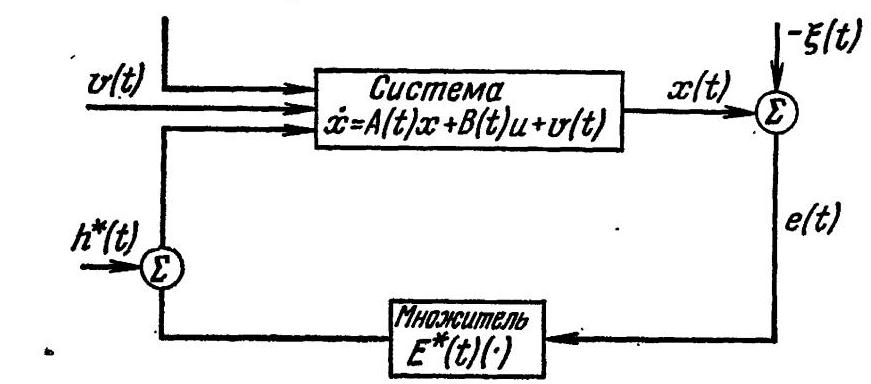
\includegraphics[max width=0.7\textwidth]{images/bo_d547k8bef24c73bgfcg0_208_419_836_871_384_0.jpg}
\end{center}
\hspace*{3em} 

Рис. 3.2. Сннтез системы с обратной связью.

выше дифференциального линейного уравнения. Заметим, что \(h\left( t\right)\) и \(E\left( t\right)\) , a тем самым и \({h}^{ * }\left( t\right)\) и E*(t),не зависят от \({x}_{0}\) .

Легко показать, что решение e(t) уравнения

\[
\dot{e} = A\left( t\right) e + B\left( t\right) \left\lbrack  {{h}^{ * }\left( t\right)  + {E}^{ * }\left( t\right) e}\right\rbrack   + \omega \left( t\right)
\]

с начальным условием е (но) =ее является оптимальным решением \({e}^{ * }\left( t\right)\) . Положим

\[
{\eta }^{\prime }\left( t\right)  = h\left( t\right)  + E\left( t\right) e\left( t\right)
\]

и проверим, что пара (e(t), η (t)) удовлетворяет системе дифферен- циальных уравнений, единственным решением которой является \(\left( {{e}^{ * }\left( t\right) ,{\eta }^{ * }\left( t\right) }\right)\) .

Таким образом, оптимальное управление, построенное как управление с обратной связью, дается выражением

\[
{u}^{ * }\left( t\right)  = {h}^{ * }\left( t\right)  + {E}^{ * }\left( t\right) e
\]

HAN

\[
{u}^{ * }\left( t\right)  = {h}^{ * }\left( t\right)  - {E}^{ * }\left( t\right) \xi \left( t\right)  + {E}^{ * }\left( t\right) x.
\]

На рис. 3.2 мы даем блок-схему управляемой системы Z+ с этим управлением.

3 амечани я. Имеется интересная интерпретация множества К для системы примера 1 (или сдвинутого множества К+ для си- стемы \({\mathcal{L}}_{ + }\) примера 2). Рассмотрим множество К в (n+1)-мерном пространстве с координатами ( \({x}^{0},x\) ); очевидно,что если система £ вполне управляема на интервале б, с < t <7, то граница множе- ства К представляет собой однозначную функцию К (х) векторного аргумента х. По определению, К(х) есть минимальное значение критерия \({C}_{0}\left( u\right)  = {x}^{0}\) при перемещении системы из \({x}_{0}\) в целевую точку \(x\) .

Вычислим теперь это минимальное значение

\[
V\left( {{x}_{0},{t}_{0}}\right)  = {x}^{*\prime }\left( T\right) G{x}^{ * }\left( T\right)  + {\int }_{{t}_{0}}^{T}\left\lbrack  {{\left\lVert \begin{array}{c} {x}^{ * } \end{array} \right\rVert}_{W}^{2} + \parallel u{\parallel }_{U}^{2}}\right\rbrack  {ds}
\]

для управляемой системы У с начальными условиями х(бо) =х,-хо Рассмотрим производную от \({x}^{\prime }E\left( t\right) x\) вдоль оптимальной траекто- рии \({x}^{ * }\left( t\right)\) ,исходящей из \({x}_{0}\) ,при оптимальном управлении \({u}^{ * }\left( t\right)  = \; = {U}^{-1}\left( t\right) {B}^{\prime }\left( t\right) E\left( t\right) {x}^{ * }\left( t\right) ;\) тогда получим

\[
{\dot{x}}^{\prime }E\left( t\right) x + {x}^{\prime }E\left( t\right) \dot{x} + {x}^{\prime }\dot{E}\left( t\right) x =
\]

\[
= {\left\lbrack  Ax + B{U}^{-1}{B}^{\prime }Ex\right\rbrack  }^{\prime }{Ex} + {x}^{\prime }E\left\lbrack  {{Ax} + B{U}^{-1}{B}^{\prime }{Ex}}\right\rbrack   + {x}^{\prime }\dot{E}x.
\]

Интегрируя и используя дифференциальное уравнение, определяю- шее \(E\left( t\right)\) , получим

\[
{x}^{*\prime }\left( T\right) E\left( t\right) {x}^{ * }\left( T\right)  - {x}_{0}^{\prime }E\left( {t}_{0}\right) {x}_{0} = {\int }_{{t}_{0}}^{T}\left\lbrack  {{\left\lVert \begin{array}{c} {x}^{ * }\left( s\right) \end{array} \right\rVert}_{W}^{2} + {\left\lVert \begin{array}{c} {u}^{ * } \end{array} \right\rVert}_{U}^{2}}\right\rbrack  {ds}.
\]

Когда основной функционал \(C\left( u\right)\) принимает значение \(C\left( u\right)  = \; = {x}^{\prime }\left( T\right) {Gx}\left( T\right)  + {x}^{0}\left( T\right)\) ,то \(V\left( {{x}_{0},{t}_{0}}\right)  =  - {x}_{0}^{\prime }E\left( {t}_{0}\right) {x}_{0}\) . Это явное вы- ражение для минимального значения критерия подтверждает ре- зультаты, полученные на основе метода динамического программи- рования в примере 4 первого раздела главы 1.

\(\Pi\) ример 3. \(C\left( u\right)  = {\zeta x}\left( T\right)  + {x}^{0}\left( T\right)\) ,где \(\zeta  \neq  0 - \phi\) иксированный \(n\) -мерный вектор-строка. В силу теоремы 5 существует единствен- ное оптимальное управление и*(t) с соответствующим решением \({x}^{ * }\left( t\right)\) . Oно определяется через единственное решение системы

\[
\dot{x} = A\left( t\right) x + B\left( t\right) {U}^{-1}\left( t\right) {B}^{\prime }\left( t\right) {\eta }^{\prime },
\]

\[
\dot{\eta } = {x}^{\prime }W\left( t\right)  - {\eta A}\left( t\right) ,
\]

удовлетворяющее начальным условиям \(x\left( {t}_{0}\right)  = {x}_{0},\eta \left( T\right)  =  - \frac{1}{2}\zeta\) , причем

\[
{u}^{ * }\left( t\right)  = {U}^{-1}\left( t\right) {B}^{\prime }\left( t\right) {\eta }^{*\prime }\left( t\right) .
\]

Мы не будем здесь строить оптимальное управление в виде цепи обратной связи (см. упражнение 9), а дадим непосредственное реше- ние двухточечной краевой задачи для системы с постоянными коэффициентами.

Пусть задана система в R2:

\[
{x}^{1} = {x}^{2},\;{x}^{2} = u,
\]

с начальными условиями \({x}^{1}\left( 0\right)  = {x}_{0}^{1},{x}^{2}\left( 0\right)  = {x}_{0}^{2}\) . Пусть критерий качества имеет вид

\[
C\left( u\right)  = {x}^{1}\left( 1\right)  + {x}^{2}\left( 1\right)  + {\int }_{0}^{1}\left\{  {{\left( {x}^{1}\left( t\right) \right) }^{2} + {\left( u\left( t\right) \right) }^{2}}\right\}  {dt}
\]

для скалярных управлений и (t) на интервале 0 с t < 1. Система для определения оптимальных решений и « и «и сии имеет вид

\[
{\dot{x}}^{1} = {x}^{2},\;{\dot{x}}^{2} = {\eta }_{2},\;{\dot{\eta }}_{1} = {x}^{1},\;{\dot{\eta }}_{2} =  - {\eta }_{1},
\]

причем хз из хзе мем как Для любых начальных условий и на льюзе и харком первози в не закуп определить решение указанной выше системы с начальными услом осмо виями ( \({x}_{0}^{1},{x}_{0}^{2},{\eta }_{10},{\eta }_{20}\) ). Действительно,

\[
{\eta }_{1}\left( t\right)  = \ddot{\varphi }\left( t\right) {x}_{0}^{1} + \varphi \left( t\right) {x}_{0}^{2} + \dddot{\varphi }\left( t\right) {\eta }_{10} + \varphi \left( t\right) {\eta }_{20},
\]

\[
{\eta }_{2}\left( t\right)  =  - \varphi \left( t\right) {x}_{0}^{1} - \varphi \left( t\right) {x}_{0}^{2} - \varphi \left( t\right) {\eta }_{10} + \varphi \left( t\right) {\eta }_{20},
\]

где

\[
\varphi \left( t\right)  = \frac{1}{\sqrt{2}}\left\lbrack  {\sin \frac{t}{\sqrt{2}}\operatorname{ch}\frac{t}{\sqrt{2}} - \cos \frac{t}{\sqrt{2}}\operatorname{sh}\frac{t}{\sqrt{2}}}\right\rbrack  .
\]

Однако \(\left( {{\eta }_{10},{\eta }_{20}}\right)\) связаны конечнымн условиями:

\[
- \frac{1}{2} = \ddot{\varphi }\left( 1\right) {x}_{0}^{1} + \dot{\varphi }\left( 1\right) {x}_{0}^{2} + \dddot{\varphi }\left( 1\right) {\eta }_{10} + \varphi \left( 1\right) {\eta }_{20},
\]

\[
- \frac{1}{2} =  - \dot{\varphi }\left( 1\right) {x}_{0}^{1} - \varphi \left( 1\right) {x}_{0}^{2} - \ddot{\varphi }\left( 1\right) {\eta }_{10} + \dddot{\varphi }\left( 1\right) {\eta }_{20}.
\]

Из этих двух уравнений определим пис и сканфинкции от \(\left( {{x}_{0}^{1},{x}_{0}^{2}}\right)\) . Таким образом, решение ( \({x}^{1}\left( t\right) ,{x}^{2}\left( t\right) ,{\eta }_{1}\left( t\right) ,{\eta }_{2}\left( t\right)\) ) вполне определяется управляемой системой 9, критерием качества C(и) и начальными условиями ( \({x}_{0}^{1},{x}_{0}^{2}\) ).

Если в каждый момент времени t из интервала О ≤ t ≤ l определить \(\left( {{\eta }_{10},{\eta }_{20}}\right)\) в зависимости от текущего или возмущенного состояния системы ( \({x}^{1}\left( t\right) ,{x}^{2}\left( t\right)\) ), то можно рассматривать управ- ление

\[
{u}^{ * }\left( t\right)  = {\eta }_{2}\left( {t,{x}_{0}^{1},{x}_{0}^{2}}\right)
\]

как управление с обратной связью.

\section*{Задачи с подвижными концами}

Существуют такие задачи управления линейными системами с интегральным критерием качества, в которых систему требуется перевести из одной заданной точки не в фиксированную точку, а в любую из точек некоторого целевого множества. Здесь мы рассмотрим те дополнительные условия, которые возникают в связи с требованием, чтобы конец траектории принадлежал целевому множеству. Снова рассмотрим систему в \({R}^{n}\) :

(L)
\[
\dot{x} = A\left( t\right)  + B\left( t\right) u,
\]

скритерием качества

\[
{C}_{0}\left( u\right)  = {x}^{0}\left( T\right)  = {\int }_{{t}_{0}}^{T}\left\lbrack  {\parallel x\left( s\right) {\parallel }_{W}^{2} + \parallel u\left( s\right) {\parallel }_{U}^{2}}\right\rbrack  {ds},
\]

как и в разделе 3.2.

Пусть G—непустое компактное выпуклое целевое множество в \({R}^{n}\) . Требуется выбрать такое управление и (t) \(\subset  {R}^{m}\) , минимизи- рующее критерий \({C}_{0}\left( u\right)\) ,которое переводило бы систему из точки \(x\left( {t}_{0}\right)  = {x}_{0}\mathrm{\;B}\) некоторую точку \(x\left( T\right)  \in  G\) . Для простоты предположим, что система 8 обладает свойством управляемости на интервале \({t}_{0} \leq  t \leq  T\) ,так что область достижимости Ё = \{ \({x}^{0}\left( T\right)\) , \(\;x\left( T\right) \}\) является замкнутым выпуклым множеством, обладающим внутрен- ними точками в R**. Если бы система 8 не обладала свойством управляемости, то все рассуждения можно было бы проводить внутри линейного многообразия \(L\left( \widehat{K}\right)\) ,натянутого на множество К в \({R}^{n + 1}\) , если только \(G\) пересекается с \(L\left( \widehat{K}\right)\) .

Множество G лежит в пространстве R" с координатами х. Рассмотрим в пространстве R"1 с координатами ( \({x}^{0},x\) ) цилиндри- ческое множество \(\widehat{G} = G \times  {R}^{1}\) . Поскольку система 𝒳 обладает свой- ством управляемости, то пересечение G с к есть замкнутое выпуклое множество. Мы хотим перевести систему из точки (0, \({x}_{0}\) ) в б ∩ K так, чтобы значение к"(7) было минимальным. Очевидно, что оптимальное управление \({u}^{ * }\left( t\right)\) существует.

Минимальное значение \({x}^{0}\) на \(\widehat{G} \cap  \dot{\widehat{K}}\) достигается в некоторой общей граничной точке \({x}^{ * }\left( T\right)  = \left( {{x}^{0 * }\left( T\right) ,{x}^{ * }\left( T\right) }\right.\) множеств G и К [если только оптимальное управление, минимизирующее \({C}_{0}\left( u\right)\) в задаче с нефиксированным целевым состоянием, не переводит систему из \({x}_{0}\) в \(G\) —этот случай сводится к примеру 1,и поэтому здесь не рассматривается]. Таким образом, оптимальное управле- ние \({u}^{ * }\left( t\right)\) ,переводящее систему из состояния \(\left( {0,{x}_{0}}\right)\) в состояние \(\widehat{{x}^{ * }}\left( T\right)\) ,дается выражением

\[
{u}^{ * }\left( t\right)  = {U}^{-1}\left( t\right) {B}^{\prime }\left( t\right) {\eta }^{*\prime }\left( t\right) .
\]

3. десь \(\widehat{\eta }\left( t\right)  = \left( {-\frac{1}{2},\eta \left( t\right) }\right)\) takoo, что

\[
\dot{\eta } = {x}^{\prime }W\left( t\right)  - {\eta A}\left( t\right) ,
\]

a \(\widehat{\eta }\left( T\right)\) -нормаль к \(\widehat{K}\) в точке \(\widehat{{x}^{ * }}\left( T\right)\) . Pacсмотрим горизонтальное поперечное сечение \(P : {x}^{0} = {x}^{\circ  * }\left( T\right)\) в \({R}^{n + 1}\) . Тогда, если считать,что \(G\) совпадает с \(\widehat{G} \cap  P\) ,можно показать,что множества G и K разделяются общей опорной \(\left( {n - 1}\right)\) -мерной плоскостью π в P. Действительно, η (Т) есть нормаль к π, причем внутренняя по отношению к G. Теми же рассуждениями, что и в теореме 5, можно показать, что задача обладает единственным оптимальным управлением \({u}^{ * }\left( t\right)\) , a \({x}^{ * }\left( t\right) ,{\eta }^{ * }\left( t\right)\) находятся как решения системы

\[
\dot{x} = A\left( t\right) x + B\left( t\right) {U}^{-1}\left( t\right) {B}^{\prime }\left( t\right) {\eta }^{\prime },\;\dot{\eta } = {x}^{\prime }W\left( t\right)  - {\eta A}\left( t\right) ,
\]

где \(x\left( {t}_{0}\right)  = {x}_{0},x\left( T\right)  \in  \partial G\) и \(\eta \left( T\right)\) -внутренняя нормаль к \(G\) в точ- ке \(x\left( T\right)\) .

Пусть целевое множество G в R" определяется неравенством \(\gamma \left( x\right)  \leq  0\) ,где \(\gamma \left( x\right)\) -выпуклая функция из \({C}^{1}\) такая,что grad \(\gamma  \neq  0\) на \(\partial G\) . Тогда граничные условия принимают вид: \(x\left( {t}_{0}\right)  = {x}_{0}\) , \(\gamma \left( {x\left( T\right) }\right)  \neq  0\) и \(\eta \left( \bar{T}\right)  =  - k\operatorname{grad}\gamma \left( {x\left( T\right) }\right)\) для некоторого \(k > 0\) . По- следнее условие называют обычно условием трансверсальности.

Пример 1. Рассмотрим линейную систему в R2:

\[
{\dot{x}}^{1} = {x}^{2},\;{\dot{x}}^{2} = u
\]

со скалярным управлением и (t) на интервале 0≤t < 1 и крите- рием качества

\[
C\left( u\right)  = {\int }_{0}^{1}{\left( u\left( t\right) \right) }^{2}{dt}
\]

Начальное состояние системы ( \({x}^{1}\left( 0\right) ,{x}^{2}\left( 0\right) ) = \left( {0, - 3}\right)\) , a целевое множество есть круг G:

\[
{\left( {x}^{1}\right) }^{2} + {\left( {x}^{2}\right) }^{2} \leq  1\text{ B }{R}^{2}.
\]

Эта система обладает свойством управляемости, и следовательно, существует единственное оптимальное управление и* (t). Мы найдем

\[
{u}^{ * }\left( t\right)  = {\eta }_{2}^{ * }\left( t\right)
\]

из системы дифференциальных уравнений

\[
{\dot{x}}^{1} = {x}^{2},\;{\dot{x}}^{2} = {\eta }_{2},\;{\dot{\eta }}_{1} = 0,\;{\dot{\eta }}_{2} =  - {\eta }_{1}
\]

с граничными условиями \({x}^{1}\left( 0\right)  = 0,{x}^{2}\left( 0\right)  =  - 3\) и условием транс- версальности

\[
\left\lbrack  \begin{array}{l} {\eta }_{1}\left( 1\right) \\  {\eta }_{2}\left( 1\right)  \end{array}\right\rbrack   =  - k\left\lbrack  \begin{array}{l} {x}^{1}\left( 1\right) \\  {x}^{2}\left( 1\right)  \end{array}\right\rbrack  \;{\mathrm{{\text{ п }\text{ р }\text{ н }}}}_{H}{\left( {x}^{1}\left( 1\right) \right) }^{2} + {\left( {x}^{2}\left( 1\right) \right) }^{2} = 1,k > 0.
\]

При любом выборе начальных данных \({\eta }_{1}\left( 0\right)  = {\eta }_{10},{\eta }_{2}\left( 0\right)  = {\eta }_{20}\) мы можем найти соответствующее единственное решение данной системы дифференциальных уравнений

\[
{\eta }_{1}\left( t\right)  = {\eta }_{10},\;{\eta }_{2}\left( t\right)  =  - {\eta }_{10}t + {\eta }_{20},
\]

\[
{x}^{1}\left( t\right)  = \frac{{\eta }_{10}{t}^{3}}{6} + \frac{{\eta }_{20}{t}^{2}}{2} - {3t},\;{x}^{2}\left( t\right)  =  - \frac{{\eta }_{10}{t}^{2}}{2} + {\eta }_{20}t - 3.
\]

Для того чтобы при t=1 удовлетворялись условия трансверсаль- ности, нужно потребовать выполнения следующих соотношений:

\[
{\eta }_{1}\left( 1\right)  = {\eta }_{10} =  - k{x}^{1}\left( 1\right)  =  - k\left( {-\frac{1}{6}{\eta }_{10} + \frac{1}{2}{\eta }_{20} - 3}\right) ,
\]

\[
{\eta }_{2}\left( 1\right)  =  - {\eta }_{10} + {\eta }_{20} =  - k{x}^{2}\left( 1\right)  =  - k\left( {-\frac{1}{2}{\eta }_{10} + {\eta }_{20} - 3}\right) ,
\]

и

\[
{\left( {\eta }_{10}\right) }^{2} + {\left( -{\eta }_{10} + {\eta }_{20}\right) }^{2} = {k}^{2}\text{ AJA HEKOТОPOТО }k > 0\text{ . }
\]

Двалинейных условия на \(\left( {{\eta }_{10},{\eta }_{20}}\right)\) дают

\[
{\eta }_{10} = \frac{{36}\left( {\frac{{k}^{2}}{2} + k}\right) }{{k}^{2} + {16k} + {12}},\;{\eta }_{20} = \frac{{12}\left( {{k}^{2} + {6k}}\right) }{{k}^{2} + {16k} + {12}}.
\]

Окончательное квадратичное условие будет выполнено, если урав- нение

\[
{k}^{4} + {32}{k}^{3} - {80}{k}^{2} - {480k} - {2448} = 0
\]

будет иметь положительный корень. Но этот многочлен четвертой степени можно разложить на множители:

\[
\left( {k - 6}\right) \left( {{k}^{3} + {38}{k}^{2} + {148k} + {408}}\right)  = 0.
\]

Таким образом, уравнение имеет положительный корень k=6, а второй множитель не имеет положительных корней. Следователь- но, \(k = 6,{\eta }_{10} = 6,{\eta }_{20} = 6\) и оптимальное управление имеет вид

\[
{u}^{ * }\left( t\right)  =  - {6t} + 6\;\left( {0 \leq  t \leq  1}\right) .
\]

Пример 2. Рассмотрим автономную систему в R", обладаю- щую свойством управляемости

(
\[
\mathcal{L}
\]
 )
\[
\dot{x} = {Ax} + {Bu},
\]

скритерием качества

\[
C\left( u\right)  = {\int }_{0}^{T}{u}^{\prime }\left( s\right) {Uu}\left( s\right) {ds}
\]

Мы хотим привести систему из состояния \(x\left( 0\right)  = {x}_{0}\) в состояние \(x\left( T\right)  =\) = 0 с минимальным показателем качества C(u). Найдем решение системы уравнений

\[
\dot{x} = {Ax} + B{U}^{-1}{B}^{\prime }{\eta }^{\prime },\;\dot{\eta } =  - {\eta A},
\]

удовлетворяющее условиям \(x\left( 0\right)  = {x}_{0},\;x\left( T\right)  = 0.\;\) Oптимальным управлением будет \({u}^{ * }\left( t\right)  = {U}^{-1}{B}^{\prime }{\eta }^{*\prime }\left( t\right)\) . Здесь \({\eta }^{ * }\left( t\right)  = {C}^{\prime }{e}^{-{At}}\) , a no- стоянный вектор \(C\) определяется из условия \(x\left( T\right)  = 0\) ,так что

\[
C =  - {\left\lbrack  \mathop{\int }\limits_{0}^{T}{e}^{-{As}}B{U}^{-1}{B}^{\prime }{e}^{-{A}^{\prime }s}ds\right\rbrack  }^{-1}{x}_{0}.
\]

Пля случая \(n = 2,m = 1\) задача прнмет вид

\[
\left\lbrack  \begin{array}{l} x \\  y \end{array}\right\rbrack   = \left\lbrack  \begin{array}{rr} 0 & 1 \\   - 1 & 0 \end{array}\right\rbrack  \left\lbrack  \begin{array}{l} x \\  y \end{array}\right\rbrack   + \left\lbrack  \begin{array}{l} 0 \\  1 \end{array}\right\rbrack  u,\;C\left( u\right)  = {\int }_{0}^{2\pi }{u}^{2}\left( s\right) {ds},
\]

II HAAO Bbl4HCJITH

\[
C =  - {\left\{  {\int }_{0}^{2\pi }\left\lbrack  \begin{array}{rr} \cos s &  - \sin s \\  \sin s & \cos s \end{array}\right\rbrack  \left\lbrack  \begin{array}{l} 0 \\  1 \end{array}\right\rbrack  \left\lbrack  \begin{array}{ll} 0 & 1 \end{array}\right\rbrack  \left\lbrack  \begin{array}{rr} \cos s & \sin s \\   - \sin s & \cos s \end{array}\right\rbrack  ds\right\}  }^{-1}\left\lbrack  \begin{array}{l} {x}_{0} \\  {y}_{0} \end{array}\right\rbrack  .
\]

Torja

\[
C = \left[ \begin{array}{c} - {x}_{0}/\pi \\   - {y}_{0}/\pi \end{array} \right]  ,
\]

H

\[
{u}^{ * }\left( t\right)  = \frac{{x}_{0}}{\pi }\sin t - \frac{{y}_{0}}{\pi }\cos t.
\]

Этот пример показывает, каким образом ошибка \(x\left( t\right)\) может быть приведена к нулю за конечный промежуток времени с минималь- ной затратой энергии. Соответствующее оптимальное управление можно выразить в явном виде как функцию начальных условий и некоторых других параметров для широкого круга линейных управляемых систем.

\section*{Регулирование на бесконечном интервале}

Если рассматриваемый интервал \({t}_{0} \leq  t \leq  T\) становится беско- нечным, т. е. Т= + ∞, то изложенная выше теория приводит к проблеме регулятора т. е. к задаче поддержания общей ошибки системы на оптимально малом уровне. Мы упростим исследование, рассматривая лишь автономные линейные системы в

(
\[
\mathcal{L}
\]
 )
\[
\dot{x} = {Ax} + {Bu},
\]

где А и B-постоянные матрицы. Далее, критерий качества для управлений \(u\left( t\right)  \subset  {R}^{m}\) на интервале 0 \(\leq  t < \infty\) имеет вид

\[
C\left( u\right)  = {\int }_{0}^{\infty }\left\lbrack  {\parallel x\left( s\right) {\parallel }_{w}^{2} + \parallel u\left( s\right) {\parallel }_{U}^{2}}\right\rbrack  {ds},
\]

где \(W = {W}^{\prime } > 0\) и \(U = {U}^{\prime } > 0\) также постоянные матрицы. До- пустимыми считаем управления и (t), измеримые на интервале \(0 \leq  t \leq  \infty\) и такие, для которых критерий качества сходится

к конечному значению. В частности, допустимыми будут все управ- ления \(u\left( t\right)\) из пространства \({L}_{2}\left( {0,\infty }\right)\) интегрируемых с квадратом функций; кроме того, отметим, что все соответствующие им реше- ния \(x\left( t\right)\) также принадлежат L, (0, ∞). В самом деле, можно по- казать, что \(\mathop{\lim }\limits_{{t \rightarrow  \infty }}x\left( t\right)  = 0\) .

Задача может и вовсе не иметь допустимых управлений, на- пример, при \(B = 0,A = I,{x}_{0} \neq  0\) . Если система х обладает свой- ством управляемости, то для того, чтобы определить допустимое управление на интервале О≤t<∞, можно взять управление, переводящее систему из точки х, в начало координат за конечное время и далее равное нулю.

В следующей ниже теореме дается синтез цепи обратной связи для оптимального управления в задаче построения регулятора. Предварительно, однако, нам придется доказать лемму Ляпунова для отрицательно определенных матриц.

Лемма. Рассмотрим уравнение, коэффициентами которого являются действительные матрицы

\[
{H}^{\prime }{E}^{\prime } + {EH} = Q,
\]

где Q = Q' > 0. Тогда решение E = E' < 0 существует в том, и только в том случае, если н—устойчивая матрица (т. е. все собственные значения матрицы H имеют отрицательную действи- тельную часть).

Доказательство. Если И —устойчивая матрица, то тре- буемое решение дается сходящимся интегралом

\[
E =  - {\int }_{0}^{\infty }{e}^{{H}^{\prime }t}Q{e}^{Ht}{dt}
\]

Очевидно, что ЕーЕ’ \(< 0\) ; интегрированием по частям получим

\[
{H}^{\prime }{E}^{\prime } =  - {\int }_{0}^{\infty }{H}^{\prime }{e}^{{H}^{\prime }t}Q{e}^{Ht}{dt} =  - {\left\lbrack  {e}^{{H}^{\prime }t}Q{e}^{Ht}\right\rbrack  }_{0}^{\infty } + {\int }_{0}^{\infty }{e}^{{H}^{\prime }t}Q{e}^{Ht}{dt}
\]

ИЛИ

\[
{H}^{\prime }{E}^{\prime } = Q - {EH},
\]

что и требовалось.

Обратно, предположим, что матрица \(E = {E}^{\prime } < 0\) есть решение нашего уравнения. Рассмотрим систему линейных дифференциаль- ных уравнений в \({R}^{n}\) :

\[
\dot{x} = {Hx}\text{ . }
\]

Продифференцируем по времени квадратичную функцию \(v\left( x\right)  = \; =  - {x}^{\prime }{Ex}\) (имеющую эллипсоидальные поверхности уровня, заключающие начало координат) вдоль решения \(x\left( t\right)  \text{ ≢ } 0\)

\[
\frac{{dv}\left( {x\left( t\right) }\right) }{dt} =  - {x}^{\prime }{Ex} - {x}^{\prime }{Ex} = {x}^{\prime }\left\lbrack  {-{H}^{\prime }{E}^{\prime } - {EH}}\right\rbrack  x.
\]

Toraa

\[
\frac{dv}{dt} =  - {x}^{\prime }{Qx} < 0
\]

и \(x\left( t\right)  \rightarrow  0\) . Таким образом, И — устойчивая матрица. Лемма до- казана.

Те орема 7. Рассмотрим автономную систему в R", обладаю- щую свойством управляемости,

(
\[
\mathcal{L}
\]
 )
\[
\dot{x} = {Ax} + {Bu},
\]

с крч𝚖ерчея качеспеа

\[
C\left( u\right)  = {\int }_{0}^{\infty }\left\lbrack  {\parallel x\left( t\right) {\parallel }_{W}^{2} + \parallel u\left( t\right) {\parallel }_{U}^{2}}\right\rbrack  {dt},\;W = {W}^{\prime } > 0,\;U = {U}^{\prime } > 0,
\]

определенным на множестве всех допустимых управлений и (t) с R’ \(\left( {0 \leq  t < \infty }\right)\) . Тогда существует единственная симметричная отри- цательно определенная матрица E, удовлетворяющая уравнению

\[
{A}^{\prime }E + {EA} + {EB}{U}^{-1}{B}^{\prime }E = W;
\]

для любого начального состояния х, о е тириествует единственное оптимальное управление и*(t), определяемое формулой

\[
{u}^{ * }\left( t\right)  = {U}^{-1}{B}^{\prime }E{x}^{ * }\left( t\right) .
\]

Таким образом, оптимальное решение x* (t) удовлетворяет асимп- тотически-устойчивой системе дифференциальных уравнений

\[
\dot{x} = \left( {A + B{U}^{-1}{B}^{\prime }E}\right) x,
\]

\(C\left( {u}^{ * }\right)  =  - {x}_{0}^{\prime }E{x}_{0}\) ecmb минимальное значение критерия качества.

Доказательство. Предположим, что существует решение \({x}^{ * }\left( t\right) ,{\eta }^{ * }\left( t\right)\) системы уравнений

\[
\dot{x} = {Ax} + B{U}^{-1}{B}^{\prime }{\eta }^{\prime }
\]

\[
\dot{\eta } = {x}^{\prime }W - {\eta A}
\]

удовлетворяющее условиям \(x\left( 0\right)  = {x}_{0},x\left( \infty \right)  = 0,\eta \left( \infty \right)  = 0\) . Тогда покажем, что соответствующее управление и « (t) = U-1 B’N’ * (t) является единственным оптимальным управлением, а х*(t)—оп- тимальной траекторией, исходящей из точки х* (0)= х. Поскольку \({x}^{ * }\left( t\right) ,{\eta }^{ * }\left( t\right)\) являются решениями автономной линейной системы, и поскольку они убывают при t/ → ∞, то они должны убывать экспоненциально, и следовательно, и*(t) является допустимым управлением.

Пусть \(\omega \left( t\right)\) — решение, соответствующее любому допустимому управлению \(u\left( t\right)\) на интервале 0 ≤ t < ∞. Положим

\[
{\omega }^{0}\left( t\right)  = {\int }_{0}^{t}\left\lbrack  {\parallel \omega \left( s\right) {\parallel }_{W}^{2} + \parallel u\left( s\right) {\parallel }_{U}^{2}}\right\rbrack  {ds},
\]

и дальше будем рассуждать так же, как в теореме 3.

Если \(u\left( t\right)\) отличается от \({u}^{ * }\left( t\right)\) на некотором положительном промежутке времени, то из доказательства теоремы 3 следует, что

\[
- \frac{1}{2}{x}^{0}\left( \infty \right)  + \eta \left( \infty \right) x\left( \infty \right)  - \eta \left( 0\right) {x}_{0} >  -
\]

\[
- \frac{1}{2}{\omega }^{0}\left( \infty \right)  + \eta \left( \infty \right) \omega \left( \infty \right)  - \eta \left( 0\right) {x}_{0}
\]

H 3HA4HT,

\[
{C}_{0}\left( {u}^{ * }\right)  < {C}_{0}\left( u\right) \text{ . }
\]

Следовательно, \({u}^{ * }\left( t\right)\) является единственным оптимальным управ- лением.

Теперь построим необходимые нам решения \({x}^{ * }\left( t\right) ,{\eta }^{ * }\left( t\right)\) ука- занной выше системы дифференциальных уравнений, используя постоянную симметричную отрицательно определенную матрицу E. Определим х* (t) как решение системы дифференциальных уравнений

\[
\dot{x} = \left( {A + B{U}^{-1}{B}^{\prime }E}\right) x
\]

сначальным условием \({x}_{0}\) и положнм

\[
{\eta }^{ * } = {x}^{*\prime }\left( t\right) E\text{ . }
\]

Тогда,используя решение \(E\) уравнения

\[
{A}^{\prime }E + {EA} + {EB}{U}^{-1}{B}^{\prime }E = W,
\]

легко проверить, что и * (t) и η* (t) являются искомыми решениями. Покажем, что у кто у место у му то му что матрица \(\left( {A + B{U}^{-1}{B}^{\prime }E}\right)\) ycroйчива.

Из условия, наложенного на \(E\) ,непосредственно следует, что

\[
{\left( A + B{U}^{-1}{B}^{\prime }E\right) }^{\prime }E + E\left( {A + B{U}^{-1}{B}^{\prime }E}\right)  = W + {EB}{U}^{-1}{B}^{\prime }E.
\]

Поскольку EBU-1B’E = \({\left( {U}^{-1}{B}^{\prime }E\right) }^{\prime }U\left( {{U}^{-1}{B}^{\prime }E}\right)  \geq  0\) как симметрич- ная матрица, то из леммы следует, что (A + BU\textasciicircum -1B’/E) есть устой- чивая матрица, что и требовалось. Чтобы вычислить оптималь- ное значение критерия качества, продифференцируем выражение \({x}^{\prime }{Ex}\) вдоль оптимальной траектории \({x}^{ * }\left( t\right)\) ; тогда получим

\[
\frac{d}{dt}\left\lbrack  {{x}^{*\prime }\left( t\right) E{x}^{ * }\left( t\right) }\right\rbrack   = {\dot{x}}^{\prime }{Ex} + {x}^{\prime }E\dot{x} =
\]

\[
= {\left( Ax + B{U}^{-1}{B}^{\prime }Ex\right) }^{\prime }{Ex} + {x}^{\prime }E\left( {{Ax} + B{U}^{-1}{B}^{\prime }{Ex}}\right) .
\]

Используя алгебраическое условие на \(E\) ,интегрированием послед- него соотношения получим

\[
{x}^{{ * }^{\prime }}\left( t\right) E{x}^{ * }\left( t\right)  - {x}_{0}^{\prime }E{x}_{0} = {\int }_{0}^{t}\left\lbrack  {{\left\lVert \begin{array}{c} {x}^{ * }\left( s\right) \end{array} \right\rVert}_{W}^{2} + {\left\lVert \begin{array}{c} {u}^{ * }\left( s\right) \end{array} \right\rVert}_{U}^{2}}\right\rbrack  {ds}.
\]

Таким образом, \(- {x}_{0}^{\prime }E{x}_{0} = G\left( {u}^{ * }\right)\) .

Вопрос о существовании и единственности отрицательно опреде- ленной матрицы E для вполне управляемых систем рассматривается в упражнениях, следующих за этим разделом. Теорема доказана.

Пример 1. Рассмотрим скалярное уравнение

\[
\dot{x} =  - x + u\left( t\right) ,\;x\left( 0\right)  = {x}_{0}
\]

н критерий качества

\[
C\left( u\right)  = {\int }_{0}^{\infty }\left\lbrack  {{x}^{2}\left( t\right)  + {u}^{2}\left( t\right) }\right\rbrack  {dt}
\]

Уравнение для определения \(E\) имеет вид

\[
\left( {-1}\right) E + E\left( {-1}\right)  + {E}^{2} = 1.
\]

Выберем \(E = 1 - \sqrt{2} < 0\) ; тогда оптимальное управление будет

\[
{u}^{ * }\left( t\right)  = \left( {1 - \sqrt{2}}\right) {x}^{ * }\left( t\right)
\]

а оптимальное решение \({x}^{ * }\left( t\right)  = {x}_{0}{e}^{-\sqrt{2}t}\) .

\section*{Упражнения}

1. Уравнение движения ротора имеет вид

\[
\dot{x} = u,
\]

где x—кинетический момент ротора, а и (t) — скалярный управляющий момент относительно неподвижной оси вращения. Если управление и (и) на интервале 0 ≤ \(t \leq\) 1 пропорционально силе тока, то общая затрачиваемая энергия равна \({\int }_{0}\alpha {u}^{2}\left( t\right) {dt}\) ,где \(\alpha  > 0\) — постоянный коэффициент. Мы хотим уменьшить на-

чальную скорость \({x}_{0}\) вращения ротора.

a) Использовать критерий качества \(C\left( u\right)  = x{\left( 1\right) }^{2} + {\int }_{0}^{1}\alpha {u}^{2}\left( t\right) {dt}\) и синтези- ровать оптимальное управление в виде управления с обратной связью. Вычис- лить минимальное значение критерия качества.

b) Использовать критерий качества \(C\left( u\right)  = x\left( 1\right)  + {\int }_{0}^{1}\alpha {u}^{2}\left( t\right) {dt}\) и вычислить его минимальное значение.

c) Рассмотреть критерий качества C (и) = д аиг и а тир правлений, при- водящих систему из состояния \({x}_{0}\) в состояние покоя. Вычислить минималь- ное значение критерия качества.

2.Уравнение движения осциллятора имеет вид

\[
\ddot{x} + x = u,
\]

где \(\left( {x,x}\right)\) -состояние системы, a \(u\left( t\right)\) -управляющая сила на интервале \(0 \leq  t \leq  {2\pi }\) . При \(t = 0\) система находилась в состоянии (0,1) и мы хотим сдви- нуть фазу колебания на \(\pi /2\) , noлучив движение \(\xi \left( t\right)  = \cos t\) . Пусть \(C\left( u\right)  = {\int }_{0}^{2\pi }\left\lbrack  {{\left( x - \cos t\right) }^{2} + {\left( \dot{x} + \sin t\right) }^{2} + {u}^{2}\left( t\right) }\right\rbrack  {dt}\) . Записать дифференциальные урав- нения для элементов матрицы обратной связи \(E\left( t\right)\) ,как в разобранных выше примерах. Заменить е (t) разностью [e(t+h)-e(t)]/h с малым шагом \(h > 0\) II HAMETHTb CXEMY YHCJEHHOТО PEILEHHA COOTBETCTBYIOLIIX PA3HOCTHILX ypashelliä.

3. Синтезировать оптимальное управление \({u}^{ * }\left( t\right)\) для задачи \(x + x = u\) с критерием качества \(C\left( u\right)  = {\int }_{0}^{\infty }\left\lbrack  {{x}^{2}\left( t\right)  + {x}^{2}\left( t\right)  + {u}^{2}\left( t\right) }\right\rbrack  {dt}\) . Найти минимум \(C\left( u\right)\)

при начальном состоянинсистемы \(x\left( 0\right)  = 0,{x}^{\prime }\left( 0\right)  = 1\) .

4. Найти оптнмальное управление \({u}^{ * }\left( t\right)\) на интервале \(0 \leq  t \leq  1\) ,которое переводило бы систему из состояния (0, 0, —3) в целевое множество \(G : {\left( {x}^{1}\right) }^{2} + {\left( {x}^{2}\right) }^{2} + {\left( {x}^{3}\right) }^{2} \leq  1\) . Система имеет вид х=и или,в Р³,

\[
{\dot{x}}^{1} = {x}^{2},\;{\dot{x}}^{2} = {x}^{3},{\dot{x}}^{3} = u,\;C\left( u\right)  = {\int }_{0}^{1}{u}^{2}\left( t\right) {dt}.
\]

5. Рассмотрим управляемую систему в R":

(L)
\[
\dot{x} = A\left( t\right) x + B\left( t\right) u
\]

с критерием качества \({C}_{0}\left( u\right)  = {\int }_{{t}_{0}}^{T}\left\lbrack  {\parallel x\left( s\right) {\parallel }_{W}^{2} + \parallel u\left( s\right) {\parallel }_{U}^{2}}\right\rbrack  {ds}\) ,заданном на множе- стве управлений и (t), определенных на интервале t, оке и Пусть \(\widehat{K} = \left\{  {{x}^{0}\left( T\right) ,x\left( T\right) }\right\}\) -множество достижимости в R**. Показать, что любой точки хек можно достигнуть, используя непрерывное управление и (t) \(\left( {{t}_{0} \leq  t \leq  T}\right)\) .

6. Рассмотрим управляющую систему в R":

\[
\dot{x} = A\left( t\right) x + B\left( t\right) u
\]

(E)скритерием качества \({\widetilde{C}}_{0}\left( u\right)  = {\left\lbrack  {\int }_{{t}_{0}}^{T}\left\lbrack  \parallel x\left( s\right) {\parallel }_{W}^{2} + \parallel \ddot{u}{\parallel }_{U}^{2}\right\rbrack  ds\right\rbrack  }^{1/2}\) , onpeдe ленным на множестве управлений \(\dot{u}\left( t\right)\) йз \({R}^{m}\) на интервале \({t}_{0} \leq  t \leq  T\) . Пусть K-мно- жество всех точек \(\left\{  {{\widetilde{C}}_{0}\left( u\right) ,{x}_{u}\left( T\right) }\right\}\) в \({R}^{n + 1}\) .

а) Доказать, что единственным оптимальным управлением и* (t) является управление,минимизирующее функционал \({C}_{0}\left( u\right)  = {\left\lbrack  {\widetilde{C}}_{0}\left( u\right) \right\rbrack  }^{2}\) .

b) Пусть g(x)—строго выпуклая функция из \({C}^{1}\) ,т. e.

\[
g\left( {\lambda {x}_{1} + \left( {1 - \lambda }\right) {x}_{2}}\right)  < {\lambda g}\left( {x}_{1}\right)  + \left( {1 - \lambda }\right) g\left( {x}_{2}\right) ,\;0 < \lambda  < 1,\;{x}_{1} \neq  {x}_{2},
\]

и пусть функция \(g\left( x\right)\) orpaничена снизу. Доказать, что если критерий качест- ва имеет вид \(C\left( u\right)  = g\left( {x\left( T\right) }\right)  + {\widetilde{C}}_{0}\left( u\right)\) , то имеется единственное оптимальное управление, а именно, \({u}^{ * }\left( t\right)  = {U}^{-1}\left( t\right) {B}^{\prime }\left( t\right) {\eta }^{*\prime }\left( t\right) \mathrm{c}\) соответствующей оптималь- ной траекторией х* (t). Здесь вектор-функция \(\left( {{x}^{ * }\left( t\right) ,{\eta }^{ * }\left( t\right) }\right)\) есть решение си- стемы уравнений

\[
\dot{x} = A\left( t\right) x + B\left( t\right) {U}^{-1}\left( t\right) {B}^{\prime }\left( t\right) {\eta }^{\prime },
\]

\[
\dot{\eta } = {x}^{\prime }W\left( t\right)  - {\eta A}\left( t\right) ,
\]

удовлетворяющее условию

\[
x\left( {t}_{0}\right)  = {x}_{0},\;\eta \left( T\right)  =  - \sqrt{{C}_{0}\left( {u}^{ * }\right) }\operatorname{grad}g\left( {x\left( T\right) }\right) .
\]

7. Рассмотрим систему в R":

(L)
\[
\dot{x} = A\left( t\right) x + B\left( t\right) u,
\]

a) \(c\) критерием качества \(C\left( u\right)  = {\int }_{{t}_{0}}^{T}\parallel x\left( s\right) {\parallel }_{W}^{2}{ds}\) , ompeделенным на мно- жестве управлений и (t) ⊂ R" (и с < t < T), удовлетворяющих ограничению \({\int }_{t}^{T}\parallel u\left( t\right) {\parallel }_{\Phi }^{2}{dt} \leq  1\) . Доказать, что в этом случае существует оптимальное уп- равление и *(t). Если W (t) > 0, то показать, что оптимальная траектория \({x}^{ * }\left( t\right)\) единственна. [У к а за ни е: использовать слабую компактность единич ного шара в \({L}_{2}\left( {{t}_{0},T}\right)\) .]

b) Пусть критерий качества \(C\left( u\right)  = {\int }_{{t}_{0}}^{T}\parallel u\left( s\right) {\parallel }_{U}^{2}{ds}\;\) задан на множестве управлений \(u\left( t\right)  \subset  {R}^{m}\left( {{t}_{0} \leq  t \leq  T}\right)\) таких, что соответствующие им решения удовлетворяют условию \({\int }_{{t}_{0}}^{T}\parallel x\left( s\right) {\parallel }_{W}^{2}{ds} \leq  1\) . Доказать существование единст- венного оптимального управления и* (t) при условии, что существует хотя бы одно допустимое управление. [Указание: пусть и «пес перситет в слабо, так что \(C\left( {u}^{\left( k\right) }\right)  \searrow  \inf C\left( u\right)\) . Total lim \(C\left( {u}^{\left( k\right) }\right)  \geq  C\left( \overrightarrow{u}\right)\) . Это последнее неравенство следует из того факта, что обобщенные коэффициенты Фурье вектор-функции и сходят. ся к соответствующим коэффициентам вектор-функции и…1

8. Предположим, что матрица E (t) = E′(t) ( \({t}_{0} \leq  t \leq  T\) ) есть решение уравнения

\[
\dot{E} = W\left( t\right)  - {A}^{\prime }\left( t\right) E - {EA}\left( t\right)  - {EB}\left( t\right) {U}^{-1}\left( t\right) {B}^{\prime }\left( t\right) E,
\]

удовлетворяющее условию \(E\left( T\right)  =  - G\) ,как и в примере 1 раздела 3.3. Дока- зать, что

\[
E\left( t\right)  = \left\lbrack  {{\psi }_{3}\left( t\right)  - {\psi }_{4}\left( t\right) G}\right\rbrack  {\left\lbrack  {\psi }_{1}\left( t\right)  - {\psi }_{2}\left( t\right) G\right\rbrack  }^{-1},
\]

rae

\[
\Psi \left( t\right)  = \left\lbrack  \begin{array}{ll} {\psi }_{1} & {\psi }_{2} \\  {\psi }_{3} & {\psi }_{4} \end{array}\right\rbrack
\]

есть фундаментальное матричное решение системы

\[
\dot{x} = A\left( t\right) x + B\left( t\right) {U}^{-1}\left( t\right) {B}^{\prime }\left( t\right) {\eta }^{\prime },
\]

\[
\dot{\eta } = {x}^{\prime }W\left( t\right)  - {\eta A}\left( t\right) ,
\]

удовлетворяющее условию \(\Psi \left( T\right)  = I\) . Написанное равенство для \(E\left( t\right)\) выпол- няется в некоторой окрестности точки t=T, точнее, до тех пор, пока матрицы \(\left\lbrack  {{\psi }_{3} - {\psi }_{4}G}\right\rbrack\) и \(\left\lbrack  {{\psi }_{1} - {\psi }_{2}G}\right\rbrack\) невырождены.

9. Рассмотрим управляемую систему в R":

(L)
\[
\dot{x} = A\left( t\right) x + B\left( t\right) u,
\]

с критерием качества \(C\left( u\right)  = {\zeta x}\left( T\right)  + {\int }_{{t}_{0}}^{T}\left\lbrack  {\parallel x\left( s\right) {\parallel }_{W}^{2} + \parallel u\left( s\right) {\parallel }_{U}^{2}}\right\rbrack  {ds}\) ,где \(\zeta\) есть ненулевой постоянный вектор. Проверить, что оптимальное управление реали- зуется в виде цепи обратной связи

\[
{u}^{ * }\left( t\right)  = {U}^{-1}\left( t\right) {B}^{\prime }\left( t\right) \left\lbrack  {h\left( t\right)  + E\left( t\right) {x}^{ * }\left( t\right) }\right\rbrack  ,
\]

rne

\[
\dot{E} = W\left( t\right)  - {A}^{\prime }\left( t\right) E - {EA}\left( t\right)  - {EB}\left( t\right) {U}^{-1}\left( t\right) {B}^{\prime }\left( t\right) E,
\]

\[
\dot{h} =  - \left\lbrack  {E\left( t\right) B\left( t\right) {U}^{-1}\left( t\right) {B}^{\prime }\left( t\right)  + {A}^{\prime }\left( t\right) }\right\rbrack  h
\]

с граничными условиями \(E\left( T\right)  = 0,h\left( T\right)  =  - {\zeta }^{\prime }/2\) .

10. Рассмотрим автономную систему в \({R}^{n}\) :

\[
\dot{x} = {Ax} + {Bu},
\]

с критерием качества \(C\left( u\right)  = {\int }_{0}^{\infty }\left\lbrack  {\parallel x\left( s\right) {\parallel }_{W}^{2} + \parallel u\left( s\right) {\parallel }_{U}^{2}}\right\rbrack  {ds}\) (см. теорему 7). Пока-

зать, что \(V\left( x\right)  =  - {x}^{\prime }{Ex}\) есть функция Ляпунова для оптимизированной системы

\[
\dot{x} = \left( {A + B{U}^{-1}{B}^{\prime }E}\right) x.
\]

Иначе говоря, проверить, что:

a) \(V\left( x\right)  > 0\) для \(x \neq  0\) и \(V\left( 0\right)  = 0\) ;

b) \(\dot{V}\left( {x\left( t\right) }\right)  < 0\) для \(x \neq  0\) .

11. Пусть \(Q = {Q}^{\prime } \geq  0\) и пусть А — действительная устойчивая (n×n)-мат- рица. Показать, что

\[
{F}_{n} = \frac{{\left( -1\right) }^{n - 1}}{n!}{\int }_{0}^{\infty }{t}^{n}{e}^{{A}^{\prime }t}{Qe}{A}^{t}{dt},\;n = 0,1,2,\ldots
\]

естъ едннственная снмметричная матрииа, удовлетворяющая уравненню

\[
{\left( {A}^{\prime }\right) }^{n + 1}F + \left( \begin{array}{c} n + 1 \\  1 \end{array}\right) {\left( {A}^{\prime }\right) }^{n}{FA} + \left( \begin{array}{c} n + 1 \\  2 \end{array}\right) {\left( {A}^{\prime }\right) }^{n - 1}F{A}^{2} + \ldots
\]

\[
\cdots  + \left( \begin{array}{c} n + 1 \\  n \end{array}\right) {A}^{\prime }F{A}^{n} + F{A}^{n + 1} = Q.
\]

Здесь биномиальные коэффициенты имеют, как обычно, вид ("+1) = \(= \frac{\left( {n + 1}\right) !}{\left( {n + 1 - r}\right) !r!}\) . [Указани е: проверить,что \({A}^{\prime }{F}_{n} + {F}_{n}A = {F}_{n - 1},{F}_{-1} = Q\) ,

Для доказательства единственности упростить вычисления, сделав преобра- зование координат \(\bar{A} = {P}^{-1}{AP},\bar{F} = {P}^{\prime }{FP},\bar{Q} = {P}^{\prime }{QP}\) .]

12. Решить уравнение \({A}^{\prime }F + {FA} = Q\) OTHOCUT是点析的 \(F = {F}^{\prime }\) ,где

\[
A = \left\lbrack  \begin{array}{rr} 0 & 1 \\   - 1 &  - 1 \end{array}\right\rbrack  ,\;Q = \left\lbrack  \begin{array}{ll} 1 & 0 \\  0 & 1 \end{array}\right\rbrack  ,
\]

13. Рассмотрим автономную систему в \({R}^{n}\) :

(L)
\[
\dot{x} = {Ax} + {Bu},
\]

こ Критерием качества

\[
C\left( u\right)  = {\int }_{0}^{\infty }\left\lbrack  {\parallel x\left( s\right) {\parallel }_{W}^{2} + \parallel u\left( s\right) {\parallel }_{U}^{2}}\right\rbrack  {ds},\;W = {W}^{\prime } > 0,U = {U}^{\prime } > 0,
\]

как и в теореме 7. Пусть и (t) (0 ≤ t < ∞) — некоторое допустимое управле. ние,т. е. управление, для которого \(C\left( u\right)  < \infty\) . Доказать, что lim x \(\left( t\right)  = 0\) . (Указание: если неше хан уны кем е уа уна любого т с о существует бес- конечное количество моментов времени \({t}_{1} \rightarrow  \infty\) ,таких,что \(\left| {x\left( {t}_{1}\right) }\right|  = \varepsilon\) ,но \(\left| {x\left( t\right) }\right|  < \frac{\varepsilon }{2}\) в некоторый момент \(t\) из интервала \({t}_{1} \leq  t \leq  {t}_{1} + \tau\) . Фиксируем достаточно малые ε> 0 и τ>0. Тогда найдется такое δ>0, что \({\int }_{{t}_{1}}^{{t}_{1} + \tau }\left| {u\left( t\right) }\right| {dt} > \delta\) . Поэтому существует \(\xi  > 0\) такое,что \({\int }_{{t}_{1}}^{{t}_{1} + \tau }\parallel u\left( t\right) {\parallel }_{U}^{2}{dt} > \xi  > 0\) для бесконечной последовательности моментов времени на 11 – 30.)

14. Вычислить симметричную матрицу обратной связи E = \(\left\lbrack  \begin{array}{ll} {e}_{1} & e \\  e & {e}_{2} \end{array}\right\rbrack\) для уп- равляемой системы

\[
\ddot{x} - {ax} = u,
\]

\(c\) критерием качества \(C\left( u\right)  = {\int }_{0}^{\infty }\left\lbrack  {{\mathbf{x}}^{\prime }W\mathbf{x} + \gamma {u}^{2}}\right\rbrack  {dt}\) ,где

\[
x = \left\lbrack  \begin{array}{l} x \\  x \end{array}\right\rbrack  ,\;W = \left\lbrack  \begin{array}{ll} {w}_{1} & w \\  w & {w}_{2} \end{array}\right\rbrack   > 0,\;\gamma  > 0.
\]

(Указание: согласно теореме 7 надо решить относительно \(E\) уравнение

\[
{A}^{\prime }E + {EA} = W - \frac{1}{\gamma }\left\lbrack  \begin{array}{ll} {e}^{2} & e{e}_{2} \\  e{e}_{2} & {e}_{2}^{2} \end{array}\right\rbrack  ,\;\text{ rie }\;A = \left\lbrack  \begin{array}{ll} 0 & 1 \\  a & 0 \end{array}\right\rbrack  ,
\]

и проверить, что если \(e =  - {\gamma a} - \sqrt{{\gamma }^{2}{a}^{2} + \gamma {w}_{1}},{e}_{1} = w - \frac{1}{\gamma }e{e}_{2} - a{e}_{2},\;{e}_{2} = \; =  - \sqrt{\gamma {w}_{2} - {2\gamma e}}\) , то матрица \(E\) является действительной и отрицательно опре- деленной).

15. Рассмотрим управляемую линейную систему в \({R}^{n}\) :

(L)
\[
x = {Ax} + {Bu},
\]

с критерием качества

\[
C\left( u\right)  = {\int }_{0}^{\infty }\left\lbrack  {\parallel x{\parallel }_{W}^{2} + \parallel u{\parallel }_{U}^{2}}\right\rbrack  {dt},\;W > 0,\;U > 0,
\]

как и в теореме 7. Доказать существование и единственность отрицательно определенной матрицы \(E\) ,удовлетворяющей уравнению

\[
W - {A}^{\prime }E - {EA} - {EB}{U}^{-1}{B}^{\prime }E = 0,
\]

H Tako共, 4ТО

\[
u = {U}^{-1}{B}^{\prime }{Ex}
\]

есть оптимальное управление, минимизирующее критерий качества, причем \(C\left( u\right)  =  - {x}_{0}^{\prime }E{x}_{0}\) . Ход доказательства намечен в следующих пунктах:

a) \(\mathrm{B}\) примере 1 раздела 3.3 симметричная матрица \(D\left( t\right)\) на интервале \(0 \leq  t \leq  T\) , yдовлетворяющая уравнению

\[
\dot{D} = W + {A}^{\prime }D + {DA} - {DB}{U}^{-1}{B}^{\prime }D,\;D\left( 0\right)  = 0,
\]

определяет усиление в цепи обратной связи E (t) =— D (— t) для соответст- вующей оптимальной управляемой системы на конечном интервале 0≤ t ≤ f . Оптимальное значение критерия качества при начальном состоянии хо равно \({x}_{0}^{\prime }D\left( T\right) {x}_{0}\) .

b) Ecлu \(0 < {T}_{1} \leq  {T}_{2}\) , то \(0 < D\left( {T}_{1}\right)  \leq  D\left( {T}_{2}\right)\) в том смысле, что \({x}^{\prime }D\left( {T}_{1}\right) x \leq  {x}^{\prime }D\left( {T}_{2}\right) x\) для всех х € \({R}^{n}\) .

c) Пусть Б — стабилизирующая матрица для системы

(L)
\[
\dot{x} = {Ax} + {Bu},\;u = \bar{D}x,
\]

т. e. такая, что матрица \(A = A + {BD}\) является устойчивой. Проверить, что сначение критерия качества для допустимого управления

\[
\bar{u}\left( t\right)  = \bar{D}{e}^{\bar{A}t}{x}_{0},\;\bar{x}\left( t\right)  = {e}^{\bar{A}t}{x}_{0}\;\text{ на }\;0 \leq  t < \infty
\]

равно \(C\left( \bar{u}\right)  = {x}_{0}^{\prime }\theta {x}_{0}\) ,где \(\theta  = {\int }_{0}^{\infty }{e}^{\bar{A}\prime t}\left\lbrack  {W + {\bar{D}}^{\prime }U\bar{D}}\right\rbrack  {e}^{\bar{A}t}{dt}\) . Cледовательно, \(D\left( T\right)  \leq  \theta\) для всех 0≤ \(T < \infty\) .

d) \(\mathop{\lim }\limits_{{T \rightarrow  \infty }}D\left( T\right)  = {D}_{\infty }\) cyществует и \(D\left( T\right)  \leq  {D}_{\infty } \leq  \theta\) .

e) Marpица \(\;{D}_{\infty }\) является решением уравнения W+A’D+DA- \(- {DB}{U}^{-1}{\bar{B}}^{\prime }D = 0\) . Тогда \(E =  - {D}_{\infty }\) и есть искомая отрицательно определен- ная матрица. Единственность решения \(E\) следует из формулы \(C\left( {u}^{ * }\right)  =  - {x}_{0}^{\prime }E{x}_{0}\) .

\section*{3.4. Интегральный выпуклый критерий качества}

Мы займемся теперь линейными управляемыми системами в R":

(L)
\[
\dot{x} = A\left( t\right) x + B\left( t\right) u,
\]

с интегральным критерием качества

\[
C\left( u\right)  = g\left( {x\left( T\right) }\right)  + {\int }_{{t}_{0}}^{T}\left\lbrack  {{f}^{0}\left( {t,x}\right)  + {h}^{0}\left( {t,u}\right) }\right\rbrack  {dt},
\]

где \(A\left( t\right) ,B\left( t\right) ,g\left( x\right) ,{f}^{0}\left( {t,x}\right) ,{h}^{0}\left( {t,u}\right)\) - непрерывные матричные \(u\) векторные функции своих аргументов \(\left( {{t}_{0} \leq  t \leq  T,x \in  {R}^{n},u \in  {R}^{m}}\right)\) . Будем также предполагать в этом разделе, что fb \(\left( {t,x}\right)\) и h’o \(\left( {t,u}\right)\) - выпуклые функции при любом фиксированном \(t\) ; кроме того,

\[
{f}^{0}\left( {t,x}\right)  \geq  0,\;{h}^{0}\left( {t,u}\right)  \geq  a{\left| u\right| }^{p}
\]

для некоторых постоянных а > 0 и p > 1. Эти предположения о положительности, которые, как будет показано в упражнениях, могут быть ослаблены, необходимы для существования оптималь- ного управления (минимизирующего критерий качества) в классе измеримых управлений с конечным значением критерия качества.

Прежде всего мы рассмотрим случай \(g\left( x\right)  \equiv  0\) . Как и раньше, мы изучим геометрию множества достижимости К/ С/С, Т/С), состоящего из конечных точек *0 всех траекторий \(\widehat{x}\left( t\right)  = \; = \left( {{x}^{0}\left( t\right) ,x\left( t\right) }\right)\) системы

\[
\dot{x} = A\left( t\right) x + B\left( t\right) u\left( t\right) ,\;{\dot{x}}^{0} = {f}^{0}\left( {t,x}\right)  + {h}^{0}\left( {t,u\left( t\right) }\right)
\]

с заданным начальным состоянием ль (н) = (0, и'). Здесь под управ- лением \(u\left( t\right)\) на интервале \({t}_{0} \leq  t \leq  T\) понимается любое допустимое управление. Используя неравенство

\[
{C}_{0}\left( u\right)  = {\int }_{{t}_{0}}^{T}\left\lbrack  {{f}^{0}\left( {t,x}\right)  + {h}^{0}\left( {t,u}\right) }\right\rbrack  {dt} \geq  a{\int }_{{t}_{0}}^{T}{\left| u\left( t\right) \right| }^{p}{dt},
\]

мы получим, что любое ограниченное измеримое управление \(u\left( t\right)\) является допустимым; кроме того, каждое допустимое управление \(u\left( t\right)\) принадлежит \({L}_{p}\left( {{t}_{0},T}\right)\) , a значит, u \({L}_{1}\left( {{t}_{0},T}\right)\) . Из предполо- жения о выпуклостй функций \({f}^{0}\left( {t,x}\right)\) и но и но и ном пе что выпуклая комбинация допустимых управлений также будет допустимым управлением.

Конец траектории \(\widehat{x}\left( T\right)\) можно вычислить, как обычно, по формуле вариации произвольных постоянных,

\[
x\left( T\right)  = \Phi \left( T\right) {x}_{0} + \Phi \left( T\right) {\int }_{{t}_{0}}^{t}{\Phi }^{-1}\left( s\right) B\left( s\right) u\left( s\right) {ds}.
\]

Кроме toro,

\[
{x}^{0}\left( T\right)  = {C}_{0}\left( u\right) .
\]

Для упрощения наших рассуждений предположим, что систе- ма \% обладает свойством управляемости на интервале б, ес t с. Отсюда будет следовать, что проекция множества K(0, T) на подпространство в \({R}^{n + 1}\) с координатой \(x\) есть все \({R}^{n}\) ,иначе нам пришлось бы все время вводить линейное многообразие, натяну- тое на \(\widehat{K}\) . Многие из наших результатов являются непосредствен- ными обобщениями теорем раздела 3.2. Однако в силу большей общности задач, рассматриваемых в этом разделе, мы не сможем получить здесь элементарный синтез оптимального управления в виде цепи обратной связи, как это делалось для квадратичных критериев качества; вместо этого мы будем сводить построение оптимального управления к двухточечной краевой задаче, которую можно решать различными численными методами.

Лемма. Рассмотрим систему в R", обладающую свойством управляемости:

(B)
\[
\dot{x} = A\left( t\right) x + B\left( t\right) u,
\]

с критерием качества Со (и и множеством достижимости КС Ргн. Тогда ортогональной проекцией К на гиперплоскость 30 в 19 все R". Далее, множество К, представляющее собой совокупность вертикальных лучей, лежит выше гиперповерхности хво-в и к репкост для всех достаточно больших |x| и некоторого постоянного а, - д.

Доказательство. Поскольку система Q вполне управляе- ма, то точки х (т) должны заполнять все пространство R", когда управление \(u\left( t\right)\) пробегает линейное пространство ограниченных измеримых функций. Так как каждое допустимое управление и (t) из \({L}_{1}\left( {{t}_{0},T}\right)\) можно аппроксимировать ограниченным управлением, и поскольку выпуклая комбинация допустимых управлений есть снова допустимое управление, то очевидно, что проекция множе- ства К на гиперплоскость \({x}^{0} = 0\) представляет собой все про- странство \({R}^{n}\) .

Пусть управление и (и) переводит систему из точки (0, и в точку \(\widehat{y} = \left( {{y}^{0},y}\right)\) в \(\widehat{K}\) . Построим управление \({u}_{\rho }\left( t\right)  = \bar{u}\left( t\right)  + \rho {u}_{\beta }\left( t\right)\) , такое, что(1)

\[
{\int }_{{t}_{0}}^{T}{\Phi }^{-1}\left( s\right) B\left( s\right) {u}_{\beta }\left( s\right) {ds} = 0
\]

и

(2)
\[
{C}_{0}\left( {u}_{p}\right)  = {y}^{0} + b
\]

для любого заданного \(b \geq  0\) . Этим будет показано, что К есть совокупность вертикальных лучей. Пусть E—замкнутое подмно- жество ненулевой меры из интервала \({t}_{0} \leq  t \leq  T\) , такое, что управ- ление \(\bar{u}\left( t\right)\) непрерывно и ограничено на \(E\) . Положим \({X}_{E}\left( t\right)  = 1\) при t из E и X в X и X и X и X и X и X X и X X и X X X X X X X X X X X X X X X X X X X X X X X X X X X X X X X X X X X X X X X X X X X X X X X X X X X X X X X X X X X X X X X X X X X X X X X X X X X X X X X X разбиение интервала \(\left\lbrack  {{t}_{0},T}\right\rbrack  {t}_{0} < {t}_{1} < {t}_{2} < \ldots  < {t}_{n + 1} < T\) , raкое,что

\[
{\int }_{{t}_{k}}^{T}{X}_{E}\left( t\right) {dt} = \frac{1}{k + 1}{\int }_{{t}_{0}}^{T}{X}_{E}\left( t\right) {dt},\;k = 1,2,\ldots ,n + 1.
\]

Тогда, используя те же обозначения, что и в лемме, предшествую- щей теореме 1, положим

\[
{u}_{\beta }^{1}\left( s\right)  = \left\lbrack  {X\left( {s,{t}_{n + 1}}\right) {\beta }_{1} + X\left( {s,{t}_{n}}\right) {\beta }_{2} + \ldots  + X\left( {s,{t}_{1}}\right) {\beta }_{n + 1}}\right\rbrack  {X}_{E}\left( t\right)
\]

H

\[
{u}_{\beta }^{j}\left( s\right)  = 0\;\text{ для }\;j = 2,3,\ldots ,m\;\text{ на }\;{t}_{0} \leq  t \leq  T.
\]

Снова выберем ненулевой вектор \(\beta  = \left\{  {{\beta }_{1},{\beta }_{2},\ldots ,{\beta }_{n + 1}}\right\}\) так,чтобы условие (1) выполнялось для \({u}_{\beta }\left( t\right)  \text{ ≢ } 0\) .

Поскольку \({u}_{\theta }\left( t\right)  = 0\) при \(t \notin  E\) и управление \(\bar{u}\left( t\right)\) orраничено на \(E\) , то управление и, но ну является допустимым при любом фикси- рованном \(\rho  \geq  0\) . Заметим,что \({C}_{0}\left( {u}_{0}\right)  = {C}_{0}\left( \bar{u}\right)  = {y}^{0},u{C}_{0}\left( {u}_{0}\right)  \geq \; \geq  a{\int }_{{t}_{0}}^{T}{\left| {u}_{\rho }\left( t\right) \right| }^{p}{dt}\) , так что

\[
\mathop{\lim }\limits_{{\rho  \rightarrow  \infty }}{C}_{0}\left( {u}_{\rho }\right)  =  + \infty
\]

Поскольку \({C}_{0}\left( {u}_{0}\right)\) непрерывно по \(\rho\) ,то существует такое \(\rho  \geq  0\) , что \({C}_{0}\left( {u}_{0}\right)  = {y}_{0} + b\) ,что и требуется.

Чтобы получить оценку, указанную в лемме, заметим, что для каждого" допустимого управления и (t)

\[
\left| {x\left( T\right) }\right|  \leq  {k}_{1} + l{\int }_{{t}_{0}}^{T}\left| {u\left( t\right) }\right| {dt}
\]

где \({k}_{1} = \left| {\Phi \left( T\right) {x}_{0}}\right|\) и \(l = \mathop{\max }\limits_{{{t}_{0} \leq  t \leq  T}}\left| {\Phi \left( T\right) {\Phi }^{-1}\left( t\right) B\left( t\right) }\right|\) . B силу выпук- лости \({\left| u\right| }^{p}\) как функции от \(\left| u\right|\) имеем неравенство

\[
{\left\lbrack  {\int }_{{t}_{0}}^{T}\left| u\left( t\right) \right| dt\right\rbrack  }^{p} \leq  {\int }_{{t}_{0}}^{T}{\left| u\left( t\right) \right| }^{p}{dt}{\left| T - {t}_{0}\right| }^{p - 1}.
\]

Takhh 06pa30M,

\[
{x}^{0}\left( T\right)  = {C}_{0}\left( u\right)  \geq  a{\left\lbrack  {\int }_{{t}_{0}}^{T}\left| u\left( t\right) \right| dt\right\rbrack  }^{p} \geq  a{\left\lbrack  \frac{\left| {x\left( T\right) }\right|  - {k}_{1}}{l}\right\rbrack  }^{p}{\left| T - {t}_{0}\right| }^{1 - p}.
\]

Otcloда следует,чтодля всех \(\left| {x\left( T\right) }\right|  \geq  2{k}_{1}\) имеем

\[
{x}^{0}\left( T\right)  \geq  \frac{a}{{\left( 2l\right) }^{p}}{\left| x\left( T\right) \right| }^{p}{\left| T - {t}_{0}\right| }^{1 - p}.
\]

Лемма доказана.

Теорема 8. Рассмотрим систему в R", обладающую свой- ством управляемости:(B)

\[
\dot{x} = A\left( t\right) x + B\left( t\right) u,
\]

с критерием качества

\[
{C}_{0}\left( u\right)  = {\int }_{{t}_{0}}^{T}\left\lbrack  {{f}^{0}\left( {t,x}\right)  + {h}^{0}\left( {t,u}\right) }\right\rbrack  {dt}.
\]

Тогда множество достижимости ЙС Спи Замкнуто и выпукло.

Доказательство. Доказательство выпуклости множества К проводится так же, как и в теореме 1. Для доказательства замк- нутости множества К воспользуемся неравенством

\[
\mathop{\lim }\limits_{{k \rightarrow  \infty }}\inf {C}_{0}\left( {u}_{k}\right)  \geq  {C}_{0}\left( \bar{u}\right)
\]

где \({u}_{k}\left( t\right)\) —последовательность управлений, слабо сходящаяся к \(\bar{u}\left( t\right)\) . Доказательство этого неравенства, которое является вы- ражением одного общего свойства выпуклых функций, приведем в заключительной части доказательства теоремы.

Рассмотрим последовательность точек \({\widehat{x}}_{k}\left( T\right)  = \left( {{x}_{k}^{0}\left( T\right) ,{x}_{k}\left( T\right) }\right)\) , соответствующую управлениям \({u}_{k}\left( t\right)\) ,и сходящуюся к \(\bar{x} = \left( {{\bar{x}}^{0},\bar{x}}\right)\) в \({R}^{n + 1}\) . Поскольку последовательность \({x}_{k}^{0}\left( T\right)  = {C}_{0}\left( {u}_{k}\right)\) orpaничена, то функции \({u}_{k}\left( t\right)\) лежат внутри некоторого замкнутого шара в банаховом пространстве \({L}_{p}\left( {{i}_{0},T}\right)\) . Следовательно,можно выбрать подпоследовательность, которую мы вновь обозначим и, к), слабо сходящуюся к й(н). Предполагая, что указанное выше неравенство верно, легко получаем, что \(\bar{u}\left( t\right)\) —допустимое управление с соот- ветствующим ему решением \(\left( {\overline{{x}^{0}}\left( t\right) ,\bar{x}\left( t\right) }\right)\) и

\[
\mathop{\lim }\limits_{{k \rightarrow  \infty }}{x}_{k}\left( t\right)  = \bar{x}\left( t\right) ,\;\mathop{\lim }\limits_{{k \rightarrow  \infty }}\inf {x}_{k}^{0}\left( T\right)  \geq  {\bar{x}}^{0}\left( T\right) .
\]

Таким образом, \(\bar{x}\left( T\right)  = \bar{x}\) и \({x}^{0}\left( T\right)  \leq  {\bar{x}}^{0}\) . Поскольку множество К представляет собой совокупность вертикальных лучей в R**, за- ключаем, что точка x принадлежит \(\widehat{K}\) , и значит, \(\widehat{K}\) замкнуто.

Докажем теперь использованное нами неравенство. В силу того, что \({u}_{k}\left( t\right)\) и \(\bar{u}\left( t\right)\) лежат в некотором замкнутом шаре пространства \({L}_{p}\left( {{t}_{0},T}\right)\) ,они должны быть равномерно ограничены в простран- CTBE \({L}_{1}\left( {{t}_{0},T}\right)\) и,значит, для нормы | \({x}_{k}\left( t\right)\) | и Z(t) также имеет место некоторая равномерная оценка. Таким образом,

\[
\mathop{\lim }\limits_{{k \rightarrow  \infty }}{\int }_{{t}_{0}}^{T}{f}^{0}\left( {t,{x}_{k}\left( t\right) }\right) {dt} = {\int }_{{t}_{0}}^{T}{f}^{0}\left( {t,\bar{x}\left( t\right) }\right) {dt}.
\]

Итак, остается лншь показать, что

\[
\mathop{\lim }\limits_{{k \rightarrow  \infty }}\inf {\int }_{{t}_{0}}^{T}{h}^{0}\left( {t,{u}_{k}\left( t\right) }\right) {dt} \geq  {\int }_{{t}_{0}}^{T}{h}^{0}\left( {t,\bar{u}\left( t\right) }\right) {dt}
\]

Пусть C — некоторое замкнутое подмножество интервала \({t}_{0} \leq  t \leq  T\) ,на котором управление й(б) непрерывно,а следова- тельно, ограничено, а S-компактный шар в R", внутри которого содержится \(\bar{u}\left( C\right)\) . Для каждого фиксированного \(t\) paccмотрим вы- пуклую гиперповерхность в R**i, описываемую уравнением

\[
{u}^{0} = {h}^{0}\left( {t,u}\right) .
\]

Для каждого \(v \in  S\) и \(t\) из интервала б, с < f > пассмотрим все опорные гиперплоскости к поверхности \({u}^{0} = {h}^{0}\left( {t,u}\right)\) в точке \(\left( {v,{h}^{0}\left( {t,v}\right) }\right)\) ,т. e. гиперплоскости

\[
{u}^{0} = \gamma \left( t\right) \left( {u - v}\right)  + {h}^{0}\left( {t,v}\right) .
\]

Множество H всех таких гиперплоскостей является компактным подмножеством (2m+1)-мерного евклидова пространства с коор- динатами (t, v, v). Поскольку ни одна из опорных гиперплоско- стей не является вертикальной, то ясно, что имеет место равно- мерная оценка

\[
\left| \gamma \right|  \leq  {C}_{1}\text{ B }H
\]

Зададимся теперь некоторым ε>0 и определим управление

\[
v\left( t\right)  = {v}_{1}{X}_{{E}_{1}}\left( t\right)  + {v}_{2}{X}_{{E}_{2}}\left( t\right)  + \ldots  + {v}_{q}{X}_{{E}_{q}}\left( t\right) \text{ для }t \in  C,
\]

\(u\;v\left( t\right)  = \bar{u}\left( t\right) ,\;\operatorname{ec\text{ л }\text{ и }}\;t\) не принадлежит С. Здесь под \({X}_{{E}_{t}}\left( t\right)\) , \({X}_{{E}_{2}}\left( t\right) \ldots {X}_{{E}_{q}}\left( t\right)\) понимаются характеристические функции непере- секающихся измеримых множеств , н. , с. , на которые разбито C, а постоянные векторы \({v}_{1},\ldots ,{v}_{q}\) выбраны так,что

\[
\left| {\bar{u}\left( t\right)  - v\left( t\right) }\right|  < \varepsilon {\left| T - {t}_{0} + 1\right| }^{-1}{C}_{1}^{-1},v\left( t\right)  \subset  S,
\]

H

\[
\left| {{h}^{0}\left( {t,\bar{u}\left( t\right) }\right)  - {h}^{0}\left( {t,v\left( t\right) }\right) }\right|  < \varepsilon {\left| T - {t}_{0} + 1\right| }^{-1}.
\]

Для каждого \(t \in  {E}_{1}\) построим опорную гиперплоскость к гипер- поверхности \({u}^{0} = {h}^{0}\left( {t,u}\right)\) в точке \(\left( {{v}_{1},{h}^{0}\left( {t,{v}_{1}}\right) }\right)\) . Пусть ее уравнение

\[
{u}^{0} - {h}^{0}\left( {t,{v}_{1}}\right)  = {\gamma }_{1}\left( t\right) \left( {u - {v}_{1}}\right) .
\]

Можно считать, что функция \({\gamma }_{1}\left( t\right)\) orраничена и измерима на \({E}_{1}\) (см. приложение к главе 2). Так как гиперповерхность \({u}^{0} = {h}^{0}\left( {t,u}\right)\) лежит выше своей опорной гиперплоскости, то получим

\[
{h}^{0}\left( {t,u}\right)  - {h}^{0}\left( {t,{v}_{1}}\right)  \geq  {\gamma }_{1}\left( t\right) \left( {u - {v}_{1}}\right) \text{ для всех }u \in  {R}^{m}\text{ . }
\]

Такнм образом,для \(t \in  {E}_{1}\) имеем

\[
{h}^{0}\left( {t,{u}_{k}\left( t\right) }\right)  - {h}^{0}\left( {t,{v}_{1}}\right)  \geq  {\gamma }_{1}\left( t\right) \left( {{u}_{k}\left( t\right)  - {v}_{1}}\right) ,\;k = 1,2,3,\ldots
\]

Используя аналогичные неравенства для каждого из множеств \({E}_{2},\ldots ,{E}_{q}\) , a также разложение

\[
\gamma \left( t\right)  = {\gamma }_{1}\left( t\right) {X}_{{E}_{1}}\left( t\right)  + {\gamma }_{2}\left( t\right) {X}_{{E}_{2}}\left( t\right)  + \ldots  + {\gamma }_{q}\left( t\right) {X}_{{E}_{q}}\left( t\right) ,
\]

получим

\[
{\int }_{C}{h}^{0}\left( {t,{u}_{k}\left( t\right) }\right) {dt} \geq  {\int }_{C}{h}^{0}\left( {t,v\left( t\right) }\right) {dt} + {\int }_{C}\gamma \left( t\right) \left( {{u}_{k}\left( t\right)  - v\left( t\right) }\right) {dt}.
\]

Для большнх \(k \rightarrow  \infty\) в силу слабой сходнмости имеем

\[
\left| {{\int }_{C}\gamma \left( t\right) \left( {{u}_{k}\left( t\right)  - \bar{u}\left( t\right)  + \bar{u}\left( t\right)  - v\left( t\right) }\right) {dt}}\right|  < \varepsilon  + \varepsilon .
\]

Кроме того, по предыдущей оценке

\[
{\int }_{C}\left| {{h}^{0}\left( {t,v\left( t\right) }\right)  - {h}^{0}\left( {t,\bar{u}\left( t\right) }\right) }\right| {dt} < \varepsilon .
\]

Поэтому

\[
{\int }_{C}{h}^{0}\left( {t,{u}_{k}\left( t\right) }\right) {dt} \geq  {\int }_{C}{h}^{0}\left( {t,\bar{u}\left( t\right) }\right) {dt} - {3\varepsilon }.
\]

Очевидно, что существует последовательность замкнутых мно- жеств \({C}_{1} \subset  {C}_{2} \subset  {C}_{3} \subset  \ldots\) . такая,что \(\mathop{\lim }\limits_{{l \rightarrow  \infty }}{C}_{l} = \left\lbrack  {{t}_{0},T}\right\rbrack\) ,и на каждом из которых управление \(u\left( t\right)\) непрерывно; повторим наши рассуж- дения для каждого из них. Поскольку последовательность \({\int }_{{t}_{0}}^{T}{h}^{0}\left( {t,{u}_{k}\left( t\right) }\right) {dt}\) orpaничена, a последовательность \({h}^{0}\left( {t,\bar{u}\left( t\right) }\right) {X}_{{c}_{l}}\left( t\right)\) монотонна по \(l\) ,то очевидно,что существует предел

\[
\mathop{\lim }\limits_{{l \rightarrow  \infty }}{\int }_{{C}_{l}}{h}^{0}\left( {t,\bar{u}\left( t\right) }\right) {dt} = {\int }_{{t}_{0}}^{T}{h}^{0}\left( {t,\bar{u}\left( t\right) }\right) {dt}.
\]

Итак, для любого заданного ε>0 существует константа С, та- кая, что

\[
{\int }_{{t}_{0}}^{T}{h}^{0}\left( {t,{u}_{k}\left( t\right) }\right) {dt} \geq  {\int }_{{c}_{l}}{h}^{0}\left( {t,{u}_{k}\left( t\right) }\right) {dt} \geq  {\int }_{{t}_{0}}^{T}{h}^{0}\left( {t,\bar{u}\left( t\right) }\right) {dt} - {4\varepsilon }
\]

для всех достаточно большнх k. Следовательно,

\[
\mathop{\lim }\limits_{{k \rightarrow  \infty }}\inf \mathop{\int }\limits_{{t}_{0}}^{T}{h}^{0}\left( {t,{u}_{k}\left( t\right) }\right) {dt} \geq  \mathop{\int }\limits_{{t}_{0}}^{T}{h}^{0}\left( {t,\bar{u}\left( t\right) }\right) {dt}.
\]

Теорема доказана.

Cледствие. Рассмотрим систему в R", обладающую свой - ством управляемости

(Z)
\[
\dot{x} = A\left( t\right) x + B\left( t\right) u
\]

с крциерчем качесмеа

\[
C\left( u\right)  = g\left( {x\left( T\right) }\right)  + {C}_{0}^{r}\left( u\right) .
\]

Если:

a) функция \(g\left( x\right)  > b,m\) . e. \(g\left( x\right)\) ограничена снизу в \({R}^{n}\) или

b) функция \(g\left( x\right)\) выпукла в \({R}^{n}\) ,

то для системы (У) существует оптимальное управление.

Доказательство. Доказательство следует из теоремы 2 и оценок, установленных в лемме предшествующей теореме 3.

Для системы У, обладающей свойством управляемости с кри- терием качества \({C}_{0}\left( u\right)\) , ynpавление \(u\left( t\right)\) ,переводящее систему из точки \(\left( {0,{x}_{0}}\right)\) в граничную точку множества К в R n+1, называется экстремальным управлением, а соответствующая траектория — экстремальной траекторией. Конечно, оптимальное управление системы Z с показателем качества C(u) = g(x(T)) + Co(u) также переводит систему по траектории \(\widehat{x}\left( t\right)  = \left( {{x}^{0}\left( t\right) ,x\left( t\right) }\right)\) в граничную точку множества К и, значит, является экстремальным. Как и раньше, мы охарактеризуем экстремальные управления с помощью принципа максимума.

В этой части теории под сопряженным решением, соответствую- щим \(u\left( t\right)\) и х би),мы будем понимать \(n + 1\) -мерный вектор-строку \(\widehat{\eta }\left( t\right)  = \left( {{\eta }_{0},\eta \left( t\right) }\right)\) ,координаты которого удовлетворяют линейной системе

(A)
\[
{\dot{\eta }}_{0} = 0,\;\dot{\eta } =  - {\eta }_{0}\frac{\partial {f}^{0}}{\partial x}\left( {t,x\left( t\right) }\right)  - {\eta A}\left( t\right) .
\]

В дополнение к обычному предположению о непрерывности, упо- мянутому в начале этого раздела, мы будем в дальнейшем пред- полагать, что функция \(\frac{\partial {f}^{0}}{\partial x}\left( {t,x}\right)\) непрерывна на интервале \({t}_{0} \leq  t \leq  T\) при \(x \in  {R}^{n}\) . Из свойства выпуклости \({f}^{0}\left( {t,x}\right)\) тогда следует,что

\[
{f}^{0}\left( {t,x}\right)  - {f}^{0}\left( {t,\bar{x}}\right)  \geq  \frac{\partial {f}^{0}}{\partial x}\left( {t,\bar{x}}\right) \left( {x - \bar{x}}\right) .
\]

Теорема 9. Рассмотрим систему в R", обладающую свойством управляемости

(L)
\[
\dot{x} = A\left( t\right) x + B\left( t\right) u,
\]

с крциерчем качеспва

\[
{C}_{0}\left( u\right)  = {\int }_{{t}_{0}}^{T}\left\lbrack  {{f}^{0}\left( {t,x}\right)  + {h}^{0}\left( {t,u}\right) }\right\rbrack  {dt}.
\]

Управление и (t) с решением х (t) будет экстремальным в том и только том случае, если существует вектор \(\widehat{\mathbf{\eta }}\left( t\right)  = \left( {{\mathbf{\eta }}_{0},\mathbf{\eta }\left( t\right) }\right)\) , yдовле- творяющий системе

(A)
\[
{\dot{\eta }}_{0} = 0,\;{\eta }_{0} < 0,\;\dot{\eta } =  - {\eta }_{0}\frac{\partial {f}_{0}}{\partial x}\left( {t,\bar{x}\left( t\right) }\right)  - {\eta A}\left( t\right) ,
\]

и такой, что принцип максимума выполняется почти всюду на интервале \(\left\lbrack  {{t}_{0},T}\right\rbrack\) :

\[
{\eta }_{0}{h}^{0}\left( {t,\bar{u}\left( t\right) }\right)  + \eta \left( t\right) B\left( t\right) \bar{u}\left( t\right)  = \mathop{\max }\limits_{u}\left\lbrack  {{\eta }_{0}{h}^{0}\left( {t,u}\right)  + \eta \left( t\right) B\left( t\right) u}\right\rbrack  .
\]

Доказательство. Пусть управление и (и) соответствующее решение \(\widehat{x}\left( t\right)  = \left( {{\bar{x}}^{0}\left( t\right) ,\bar{x}\left( t\right) }\right)\) ,и сопряженное решение 1, \(\left( t\right)  = \left( {{\eta }_{0},\eta \left( t\right) }\right)\) удовлетворяют системе

\[
\left( \widehat{\mathcal{L}}\right)
\]

\[
= A\left( t\right) x + B\left( t\right) \bar{u}\left( t\right) ,
\]

\[
{\dot{x}}^{0} = {f}^{0}\left( {t,x}\right)  + {h}^{0}\left( {t,\bar{u}\left( t\right) }\right) ,\;\widehat{x}\left( {t}_{0}\right)  = \left( {0,{x}_{0}}\right) ,
\]

а также системе A при по с 0 и сформулированному выше прин- ципу максимума. Мы покажем, что

\[
\widehat{\eta }\left( T\right) \widehat{x}\left( t\right)  \geq  \widehat{\eta }\left( T\right) \widehat{\omega }\left( T\right) ,
\]

где \(\widehat{\omega }\left( t\right)  = \left( {{\omega }^{0}\left( t\right) ,\omega \left( t\right) }\right)\) есть решение, соответствующее произволь- ному допустимому управлению и (t). Из этого неравенства сле- дует,что точка \(\widehat{x}\left( T\right)\) лежит на границе множества К и что век- тор \(\widehat{\eta }\left( T\right)\) есть внешняя нормаль к \(\widehat{K}\) в этой точке.

Из уравнений 20 и д следует, что

\[
\frac{d}{dt}\left\lbrack  {\widehat{\eta }\left( t\right) \widehat{\omega }\left( t\right) }\right\rbrack   = {\eta }_{0}{\dot{\omega }}^{0} + \eta \dot{\omega } + \eta \dot{\omega }
\]

H

\[
\widehat{\eta }\left( T\right) \widehat{\omega }\left( T\right)  - \widehat{\eta }\left( {t}_{0}\right) {\widehat{x}}_{0} =
\]

\[
= {\int }_{{t}_{0}}^{T}\left\{  {{\eta }_{0}\left\lbrack  {{f}^{0}\left( {t,\omega }\right)  - \frac{\partial {f}^{0}}{\partial x}\left( {t,\bar{x}}\right) \omega }\right\rbrack   + \left\lbrack  {{\eta }_{0}{h}^{0}\left( {t,u}\right)  + {\eta Bu}}\right\rbrack  }\right\}  {dt}.
\]

Пусть теперь управление \(u\left( t\right)\) равняется \(\bar{u}\left( t\right)\) , a решение \(\widehat{\omega }\left( t\right)\) равно \(\widehat{x}\left( t\right)\) ; тогда получим

\[
\widehat{\eta }\left( T\right) \widehat{x}\left( T\right)  - \widehat{\eta }\left( {t}_{0}\right) {\widehat{x}}_{0} =
\]

\[
= {\int }_{{t}_{0}}^{T}\left\{  {{\eta }_{0}\left\lbrack  {{f}^{0}\left( {t,\overrightarrow{x}}\right)  - \frac{\partial {f}^{0}}{\partial x}\left( {t,\overrightarrow{x}}\right) \overrightarrow{x}}\right\rbrack   + \left\lbrack  {{\eta }_{0}{h}^{0}\left( {t,\overrightarrow{u}}\right)  + {\eta Bu}}\right\rbrack  }\right\}  {dt}.
\]

Из прннципа макснмума и условия выпуклости следуег, что

\[
{\eta }_{0}{h}^{0}\left( {t,\bar{u}\left( t\right) }\right)  + \eta \left( t\right) B\left( t\right) \bar{u}\left( t\right)  \geq  {\eta }_{0}{h}^{0}\left( {t,u\left( t\right) }\right)  + \eta \left( t\right) B\left( t\right) u\left( t\right)
\]

H

\[
{f}^{0}\left( {t,\omega }\right)  - {f}^{0}\left( {t,\bar{x}}\right)  \geq  \frac{\partial {f}_{0}}{\partial x}\left( {t,\bar{x}}\right) \left( {\omega  - \bar{x}}\right) ,
\]

откуда вытекает, что \(\widehat{\eta }\left( T\right) \widehat{x}\left( T\right)  \geq  \widehat{\eta }\left( T\right) \widehat{\omega }\left( T\right)\) . Tem caмым \(\bar{u}\left( t\right)\) является экстремальным управлением.

Обратно, предположим, что й (н) — экстремальное управление, так что соответствующая траектория \(\widehat{x}\left( t\right)  = \left( {\bar{{x}^{0}}\left( t\right) ,\bar{x}\left( t\right) }\right)\) ведет из точки \(\left( {0,{x}_{0}}\right)\) в точку \(\widehat{x}\left( T\right)\) ,лежащую на границе множества К. \(\Pi\) ycть \(\widehat{\eta }\left( T\right)  = \left( {{\eta }_{0},\eta \left( T\right) }\right)\) -внешняя нормаль к K в точке X(T). Очевидно, что \({\eta }_{0} < 0\) ; для простоты примем п, \(\widehat{\eta }\left( t\right)\) как решение сопряженной системы A с заданными гранич- ными условиями η(T) при \(t = T\) . Требуется доказать, что

\[
- {h}^{0}\left( {t,\bar{u}\left( t\right) }\right)  + \eta \left( t\right) B\left( t\right) \bar{u}\left( t\right)  = \mathop{\max }\limits_{u}\left\lbrack  {-{h}^{0}\left( {t,u}\right)  + \eta \left( t\right) B\left( t\right) u}\right\rbrack
\]

почти всюду на интервале \({t}_{0} \leq  t \leq  T\) .

Доказательство усложняется из-за того, что сопряженная си- стема д зависит от основного решения лс тоноы обойти эту трудность, мы введем одно построение, которое в дальнейшем будет применено при доказательстве принципа максимума для наиболее общих нелинейных систем. Сущность этого метода со- CТОUT B ТОM, чТО B Teчение некоторого короткого промежутка времени \({t}_{1} \leq  t \leq  {t}_{1} + \varepsilon\) на управление и (t) накладывается импульс- ное возмущение; на этом промежутке управление и вы не удов- летворяет принципу максимума. Возмущенное управление и зи (не дает приращение, выражаемое формулой \({\int }_{{t}_{0}}^{T}\left\lbrack  {{\eta }_{0}{h}^{0}\left( {t,u}\right)  + \eta \left( t\right)  \times  }\right. \; \times  B\left( t\right) u\rbrack {dt}\) при вычислении \(\widehat{\eta }\left( T\right) \widehat{\omega }\left( T\right)\) ,что противоречит пред- положению о том, что \(\widehat{x}\left( T\right)\) лежит на границе К.

Изложим теперь это доказательство подробно. Предположим, что управление и (н) не удовлетворяет принципу максимума в те- чение некоторого положительного промежутка времени из интер- вала \({t}_{0} \leq  t \leq  T\) . Oпределим управление и (t) по формуле

\[
- {h}^{0}\left( {t,\widetilde{u}\left( t\right) }\right)  + \eta \left( t\right) B\left( t\right) \widetilde{u}\left( t\right)  = \mathop{\max }\limits_{u}\left\lbrack  {-{h}^{0}\left( {t,u}\right)  + \eta \left( t\right) B\left( t\right) u}\right\rbrack  .
\]

Очевидно, что управление и (и) ограничено, и его можно выбрать измеримым, как показано в приложении к главе 2. Пусть C- компактное подмножество ненулевой меры из интервала \({t}_{0} < t < T\) , на котором управления \(\bar{u}\left( t\right)\) и \(\bar{u}\left( t\right)\) непрерывны,и удовлетворяют неравенству

\[
- {h}^{0}\left( {t,\bar{u}\left( t\right) }\right)  + \eta \left( t\right) B\left( t\right) \bar{u}\left( t\right)  <  - {h}^{0}\left( {t,\widetilde{u}\left( t\right) }\right)  + \eta \left( t\right) B\left( t\right) \widetilde{u}\left( t\right)  - \delta
\]

для некоторого постоянного \(\delta  > 0\) . Выберем момент и сконча которого множество \(\left( {{t}_{1},{t}_{1} + \varepsilon }\right)  \cap  C\) имеет меру ε[1+O(ε)] для малого ε> 0 \(\left\lbrack  {3\text{ десь }\mathop{\lim }\limits_{{\varepsilon  \rightarrow  0}}O\left( \varepsilon \right)  = 0}\right\rbrack\) . Определим возмущенное управ- яение

\[
{u}_{\varepsilon }^{ * }\left( t\right)  = \left\{  \begin{array}{l} \widetilde{u}\left( t\right) \;\text{ На }\;C \cap  \left( {{t}_{1},{t}_{1} + \varepsilon }\right) , \\  \bar{u}\left( t\right) \text{ в остальной чати ннтервала }{t}_{0} \leq  t \leq  T. \end{array}\right.
\]

Тогда, для достаточно малых ε> 0, решение ёсей). соответствую- mee управлению \({u}_{\varepsilon }^{ * }\left( t\right)\) , paвномерно аппроксимирует \(\widehat{x}\left( t\right)\) . Toчнее, легко показать, что

\[
\left| {\widehat{{x}_{\varepsilon }^{ * }}\left( t\right)  - \widehat{x}\left( t\right) }\right|  < {k\varepsilon }\text{ для некоторого }k > 0
\]

на интервале \({t}_{0} \leq  t \leq  T\) . Поскольку производная д \(\frac{\partial {f}^{0}}{\partial x}\left( {t,x}\right)\) непре- рывна, то

\[
\left| {{f}^{0}\left( {t,{x}_{\varepsilon }^{ * }\left( t\right) }\right)  - {f}^{0}\left( {t,\bar{x}\left( t\right) }\right)  - \frac{\partial {f}^{0}}{\partial x}\left( {t,\bar{x}\left( t\right) }\right) \left( {{x}_{\varepsilon }^{ * }\left( t\right)  - \bar{x}\left( t\right) }\right) }\right|  < {\varepsilon O}\left( \varepsilon \right) .
\]

Из предыдущих вычислений для \(\widehat{\eta }\left( T\right) \widehat{\omega }\left( T\right)\) следуег,что

\[
\widehat{\eta }\left( T\right) \widehat{x}\left( T\right)  - \widehat{\eta }\left( T\right) {\widehat{x}}_{\varepsilon }^{ * }\left( T\right)  \leq
\]

\[
\leq  {\int }_{{t}_{0}}^{T}\left\lbrack  {{f}^{0}\left( {t,{x}_{\varepsilon }^{ * }\left( t\right) }\right)  - {f}^{0}\left( {t,\bar{x}\left( t\right) }\right)  - \frac{\partial {f}^{0}}{\partial x}\left( {t,\bar{x}\left( t\right) }\right) \left( {{x}_{\varepsilon }^{ * }\left( t\right)  - \bar{x}\left( t\right) }\right) }\right\rbrack  {dt} -
\]

\[
- {\delta \varepsilon }\left\lbrack  {1 + O\left( \varepsilon \right) }\right\rbrack  .
\]

Тогда,для достаточно малого \(\varepsilon  > 0\)

\[
\widehat{\eta }\left( T\right) \widehat{}{\widehat{x}}_{\varepsilon }^{ * }\left( T\right)  > \widehat{\eta }\left( T\right) \widehat{x}\left( T\right) .
\]

Однако это невозможно, поскольку у (т) является внешней нор- малью к \(\widehat{K}\) в граничной точке x́(). Cледовательно, экстремальное управление \(\bar{u}\left( t\right)\) должно удовлетворять принципу максимума с сопряженным решением η(t). Теорема доказана.

Следствие. Рассмотрим систему в R", обладающую свой- ством управляемости:

\[
f\left( \mathcal{D}\right)
\]

\[
\dot{x} = A\left( t\right) x + B\left( t\right) u
\]

с крциерцем качеспеа

\[
C\left( u\right)  = g\left( {x\left( T\right) }\right)  + {\int }_{{t}_{0}}^{T}\left\lbrack  {{f}^{0}\left( {t,x}\right)  + {h}^{0}\left( {t,u}\right) }\right\rbrack  {dt},
\]

где ъфункция \(g\left( x\right)\) ъыпукла, а функция \({h}^{0}\left( {t,u}\right)\) строго выпукла, т. е. для 0 < λ < 1 \textasciitilde  u = \({u}_{1}\) = 0 и для любого фиксированного t

\[
{h}^{ \bullet  }\left( {t,\lambda {u}_{1} + \left( {1 - \lambda }\right) {u}_{2}}\right)  < \lambda {h}^{ \bullet  }\left( {t,{u}_{1}}\right)  + \left( {1 - \lambda }\right) {h}^{ \bullet  }\left( {t,{u}_{2}}\right) .
\]

Тогда любые два экстремальных управления, переводящие систему из точки \(\left( {0,{x}_{0}}\right)\) в одну и ту же граничную точку множества \(\widehat{K}\) ，должны совпадать почти всюду. Кроме того, существует единственное оптимальное управление.

Доказательство. Пусть и (t)—экстремальное управление, a \(\widehat{x}\left( t\right)  = \left( {\bar{{x}^{0}}\left( t\right) ,\bar{x}\left( t\right) }\right)\) -coopbertствующее решение. Пусть далее \(\widehat{\eta }\left( t\right)  = \left( {-1,\eta \left( t\right) }\right)\) — соответствующее сопряженное решение, так что вектор \(\widehat{\eta }\left( T\right)\) является внешней нормалью к \(\widehat{K}\) в точке \(\widehat{x}\left( T\right)\) . Тогда управление \(\bar{u}\left( t\right)\) удовлетворяет принципу максимума

\[
- {h}^{0}\left( {t,\bar{u}\left( t\right) }\right)  + \eta \left( t\right) B\left( t\right) \bar{u}\left( t\right)  = \mathop{\max }\limits_{u}\left\lbrack  {-{h}^{0}\left( {t,u}\right)  + \eta \left( t\right) B\left( t\right) u}\right\rbrack   = m\left( t\right) .
\]

Пусть теперь управление \(u\left( t\right)\) вдоль соответствующего реше- ния \(\widehat{\omega }\left( t\right)\) переводит систему из \(\left( {0,{x}_{0}}\right)\) в ту же самую точку \(\widehat{\omega }\left( T\right)  = \widehat{x}\left( T\right)\) . Если управление \(u\left( t\right)\) не удовлетворяет принципу максимума при заданном \(\eta \left( t\right)\) , то

\[
{\int }_{{t}_{0}}^{T}\left\lbrack  {-{h}^{0}\left( {t,\bar{u}\left( t\right) }\right)  + \eta \left( t\right) B\left( t\right) \bar{u}\left( t\right) }\right\rbrack  {dt} >
\]

\[
> {\int }_{{t}_{0}}^{T}\left\lbrack  {-{h}^{0}\left( {t,u\left( t\right) }\right)  + \eta \left( t\right) B\left( t\right) u\left( t\right) }\right\rbrack  {dt}\text{ . }
\]

Тогда вычисления,проведенные в теореме 9, показывают, что

\[
\widehat{\eta }\left( T\right) \widehat{x}\left( T\right)  > \widehat{\eta }\left( T\right) \widehat{\omega }\left( T\right)  = \widehat{\eta }\left( T\right) \widehat{x}\left( T\right) ,
\]

что невозможно. Таким образом, заключаем, что управления \(\bar{u}\left( t\right)\) и \(u\left( t\right)\) удовлетворяют принципу максимума почти всюду на интервале \({t}_{0} \leq  t \leq  T\) .

Рассмотрим теперь управление \(\frac{1}{2}\left\lbrack  {\bar{u}\left( t\right)  + u\left( t\right) }\right\rbrack\) . Из строгой выпуклости \({h}^{0}\left( {t,u}\right)\) cледует,что

\[
- {h}^{0}\left( {t,\frac{1}{2}\bar{u}\left( t\right)  + \frac{1}{2}u\left( t\right) }\right)  + \eta \left( t\right) B\left( t\right) \frac{1}{2}\left\lbrack  {\bar{u}\left( t\right)  + u\left( t\right) }\right\rbrack   >
\]

\[
> \frac{1}{2}m\left( t\right)  + \frac{1}{2}n \tag{t}
\]

всюду, где \(\bar{u}\left( t\right)  \neq  u\left( t\right)\) . Из предыдущих рассуждений заключаем, что управления \(\bar{u}\left( t\right)\) и \(u\left( t\right)\) совпадают почти всюду.

Поскольку \(g\left( x\right)\) есть выпуклая функция, то должно сущест- вовать оптимальное управление \({u}^{ * }\left( t\right)\) ,являющееся экстремальным и переводящее систему из точки (0, \({x}_{0}\) ) в то подмножество гра- ницы множества R, где функционал \({x}^{0} + g\left( x\right)\) достигает своего минимума. Из теоремы 5 следует, что функционал у му не и слу с усп достигать минимума лишь в одной точке P множества К. Следо- вательно, \({u}^{ * }\left( t\right)\) есть единственное экстремальное управление, пе- реводящее систему из точки (0, \({x}_{0}\) ) в точку \(P\) ,что и требовалось доказать.

3 амечания. Даже в случае, если во не является строго выпуклой функцией, можно получить вполне определенное экстремальное управление и*(*, η (t) для каждого заданного со- пряженного решения η(t). А именно, для каждого фиксирован- ного \(t\) и заданного \(\eta\) следует выбрать \({u}^{ * }\left( {t,\eta }\right)\) ,исходя из прин- ципа максимума

\[
- {h}^{0}\left( {t,{u}^{ * }}\right)  + {\eta B}\left( t\right) {u}^{ * } = \mathop{\max }\limits_{u}\left\lbrack  {-{h}^{0}\left( {t,u}\right)  + {\eta B}\left( t\right) u}\right\rbrack  .
\]

Если функция \({h}^{0}\left( {t,u}\right)\) строго выпукла при каждом \(t\) , ro прин- цип максимума однозначно определяет управление и*(t, η). Одна- ко, если даже в он (н и) просто выпуклая функция, то можно одно- значно определить \({u}^{ * }\left( {t,\eta }\right)\) ,выбрав среди точек \({R}^{m}\) , yдовлетворя- ющих принципу максимума, точку с наименьшими координатами. Иначе говоря, выберем и « (t, η) = (u*n, u*a, u*n ) так, чтобы и*1 было минимальным из всех возможных решений принципа максимума, затем выберем и* инимальным среди всех решений с выбранным значением и" и так далее, пока не получим \({u}^{ * }\left( {t,\eta }\right)\) . Если вектор-функция \(\eta \left( t\right)\) непрерывна, \({\tau o}{u}^{ * }\left( t\right)  = \; = {u}^{ * }\left( {t,\eta \left( t\right) }\right)\) будет приемлемым управлением (см. приложение к главе 2).

Следующая теорема показывает, что и*(t, η) можно интерпре- тировать как оптимальное управление, определенное на основе синтеза цепи обратной связи.

Teopeма 10. Рассмотрим управляемую систему в R"

(L)
\[
\dot{x} = A\left( t\right) x + B\left( t\right) u,
\]

с крциерцем качеспва

\[
C\left( u\right)  = g\left( {x\left( T\right) }\right)  + {\int }_{{t}_{0}}^{T}\left\lbrack  {{f}^{0}\left( {t,x}\right)  + {h}^{0}\left( {t,u}\right) }\right\rbrack  {dt}.
\]

Предположим, что функция g(x)∈C1 выпукла в R". Тогда суще- ствует решение \({x}^{ * }\left( t\right) ,{\eta }^{ * }\left( t\right)\) cucmemы уравнений

\[
\dot{x} = A\left( t\right) x + B\left( t\right) {u}^{ * }\left( {t,\eta }\right) ,
\]

\[
\dot{\eta } = \frac{\partial {f}^{0}}{\partial x}\left( {t,x}\right)  - {\eta A}\left( t\right) ,
\]

такое, что x(t, o)=x, η(T)=-grad g(x(T)). Здесь управление \({u}^{ * }\left( {t,\eta }\right)\) onpеделено из принципа максимума

\[
- {h}^{0}\left( {t,{u}^{ * }}\right)  + {\eta B}\left( t\right) {u}^{ * } = \mathop{\max }\limits_{u}\left\lbrack  {-{h}^{0}\left( {t,u}\right)  + {\eta B}\left( t\right) u}\right\rbrack  ,
\]

\(a{u}^{ * }\left( t\right)  = {u}^{ * }\left( {t,{\eta }^{ * }\left( t\right) }\right)\) является оптимальным управлением с coom- ветствующей оптимальной траекторией х*(t).

Если функция \({h}^{0}\left( {t,u}\right)\) строго выпукла при любом \(t\) , mo реше- ние \({x}^{ * }\left( t\right) ,{\eta }^{ * }\left( t\right) e\partial u\) нственно, \(u{u}^{ * }\left( t\right)\) есть \(e\) динственное опти- мальное управление.

Доказательство. Срассмотрим гиперповерхности \({S}_{c}\) : \({x}^{0} + g\left( x\right)  = C\) в \({R}^{n + 1}\) . Тогда, \(\operatorname{\text{ к }\text{ а }\text{ к }}u\) в теореме 5, cyществует един- ственная гиперповерхность \({S}_{m}\) из этого семейства, такая, что \$ касается \(\widehat{K}\) , a \(m\) есть оптимальное значение критерия качества. \(\Pi\) ycть \({\widehat{\eta }}^{ * }\left( T\right)  = \left( {-1,{\eta }^{ * }\left( T\right) }\right)\) -нормаль к касательной гиперплоско- CTH \(K{S}_{m}\) в некоторой точке \(P \in  {S}_{m} \cap  \widehat{K}\) . Пусть,далее, \({u}^{ * }\left( t\right)\) - экстремальное управление, переводящее систему из точки (0, \%) в точку \(P = {\widehat{x}}^{ * }\left( T\right)\) вдоль траектории \({\widehat{x}}^{ * }\left( t\right)  = \left( {{x}^{0 * }\left( t\right) ,{x}^{ * }\left( t\right) }\right)\) . Onpe- делим \({\eta }^{ * }\left( t\right)  = \left( {-1,{\eta }^{ * }\left( t\right) }\right)\) как решение системы

\[
\dot{\eta } = \frac{\partial {f}^{0}}{\partial x}\left( {t,{x}^{ * }\left( t\right) }\right)  - {\eta A}\left( t\right) ,
\]

удовлетворяющее условию \({\eta }^{ * }\left( T\right)  =  - \operatorname{grad}g\left( {{x}^{ * }\left( T\right) }\right)\) .

Из теоремы 9 следует, что управление и"(t) удовлетворяет принципу максимума с сопряженным решением у ме. и * (t) = \(= {u}^{ * }\left( {t,{\eta }^{ * }\left( t\right) }\right)\) . Таким образом, \({x}^{ * }\left( t\right) ,{\eta }^{ * }\left( t\right)\) есть искомое решение указанной выше нелинейной краевой задачи.

Если h0 (t, u)—crporo выпуклая функция от и при любом фиксированном \(t\) ,то множество \({S}_{m} \cap  \widehat{K}\) содepжит единственную точку P, как показано в процессе доказательства теоремы 5. Тогда из следствия из теоремы 9 вытекает, что оптимальное управление \({u}^{ * }\left( t\right)\) и соответствующее ему решение к’мене увинствен- ны. Точно так же и уч(н) определяется однозначно, как решение линейной системы дифференциальных уравнений с граничными условиями η (T) = — grad \(g\left( {{x}^{ * }\left( T\right) }\right)\) . Теорема доказана.

Примечания к задаче с подвижными концами. Рассмотрим систему в R", обладающую свойством управляемости

(Y)
\[
\dot{x} = A\left( t\right) x + B\left( t\right) u,
\]

скритерием качества

\[
C\left( u\right)  = g\left( {x\left( T\right) }\right)  + {C}_{0}\left( u\right) ,
\]

как и в теореме 10. Мы хотим перевести систему из начального состояния \({x}_{0}\) в заданное целевое состояние \({x}_{1} \in  {R}^{n}\) с минималь- ным значением критерия качества. Будем считать \({h}^{0}\left( {t,u}\right)\) crporo выпуклой функцией при любом фиксированном t из интервала \({t}_{0} \leq  t \leq  T\) .

При этих условиях система обладает единственным оптималь- ным управлением и" (t), переводящим ее из точки и, в точку х,. Действительно, рассмотрим подмногообразие 1: \(x = {x}_{1}\) в \({R}^{n + 1}\) . Здесь \(l \cap  \widehat{K}\) есть отрезок вертикальной прямой. Тогда и*(t) переводит систему из точки (0, \({x}_{0}\) ) в точку ( \({x}^{0 * }\left( T\right) ,{x}_{1}\) ), \(\Gamma\) дe \({x}^{0 * }\left( T\right)\) есть ca- мая низкая точка отрезка \(l \cap  \widehat{K}\) и \(C\left( {u}^{ * }\right)  = g\left( {x}_{1}\right)  + {x}^{0 * }\left( T\right)\) . Далее, если \({x}^{ * }\left( t\right) ,{\eta }^{ * }\left( t\right)\) -некоторое решение системы уравнений

\[
\dot{x} = A\left( t\right) x + B\left( t\right) {u}^{ * }\left( {t,\eta }\right) ,
\]

\[
\dot{\eta } = \frac{\partial {f}^{0}}{\partial x}\left( {t,x}\right)  - {\eta A}\left( t\right) ,
\]

такое,что \(x\left( {t}_{0}\right)  = {x}_{0},x\left( T\right)  = {x}_{1}\) , ro \({u}^{ * }\left( t\right)  = {u}^{ * }\left( {t,{\eta }^{ * }\left( t\right) }\right)\) , a \({x}^{ * }\left( t\right)\) пред- ставляет собой оптимальное решение, соответствующее и" (н).

Рассмотрим теперь при тех же предположениях [система ] обладает свойством управляемости на \({t}_{0} \leq  t \leq  T\) и \({h}^{ * }\left( {t,u}\right)\) crporo выпуклая функция от и при любом t] задачу о приведении си- стемы из начальной точки \({x}_{0}\) в фиксированное компактное вы- пуклое целевое множество \(G : \gamma \left( x\right)  \leq  0\) в \({R}^{n}\) . Здесь \(\gamma \left( x\right)\) — некоторая выпуклая функция класса \({C}^{1}\) ,причем grad \(\gamma \left( x\right)  \neq  0\) на границе G, представляющей собой гладкую выпуклую гиперповерхность. Как и в рассуждениях раздела 3.3, рассмотрим цилиндрическое множество \(\widehat{G} = G \times  {R}^{1}\) B \(n + 1\) -мерном пространстве с координатами \(\left( {{x}^{0},x}\right)\) . Поскольку система 8 вполне управляема, то множество G пере- секается с множеством \(\widehat{K}\) по замкнутому выпуклому множеству, и значит, существует оптимальное управление и (t), переводящее систему из состояния \({x}_{0}\) в \(G\) и минимизирующее функционал \(C\left( u\right)\) .

Для того чтобы еще более упростить задачу, предположим, что \(g\left( x\right)  \equiv  0\) ,так что \(C\left( u\right)  = {C}_{0}\left( u\right)\) . Тогда минимальное значение \({x}^{0}\) достигается в \(\widehat{G} \cap  \widehat{K}\) в единственной общей граничной точке \(\widehat{{x}^{ * }}\left( T\right)  = \left( {{x}^{0 * }\left( T\right) ,{x}^{ * }\left( T\right) }\right)\) [если только оптимальное управление, ми- нимизирующее \({C}_{0}\left( u\right)\) вне зависимости от целевого состояния, не будет все же переводить систему из точки х, в G; этот особый случай, соответствующий равенству η (T) =0 в теореме 10, мы исключаем из рассмотрения, так как он имеет место тогда и только тогда, когда излагаемый ниже метод не дает решения за- дачи]. Таким образом, существует единственное оптимальное управление \({u}^{ * }\left( t\right)\) , переводящее систему из точки \({x}_{0}\) в G, причем соответствующая траектория заканчивается в точке \({\widehat{x}}^{ * }\left( T\right)\) . В точ- ности как в разделе 3.3, можно получить управление и*(t) из любого решения \({x}^{ * }\left( t\right) ,{\eta }^{ * }\left( t\right)\) системы

\[
\dot{x} = A\left( t\right) x + B\left( t\right) {u}^{ * }\left( {t,\eta }\right) ,
\]

\[
\dot{\eta } = \frac{\partial {f}^{0}}{\partial x}\left( {t,x}\right)  - {\eta A}\left( t\right) ,
\]

удовлетворяющего условию \(x\left( {t}_{0}\right)  = {x}_{0},\gamma \left( {x\left( T\right) }\right)  = 0\) , a также усло- вию трансверсальности

\[
\eta \left( T\right)  =  - k\operatorname{grad}\gamma \left( {x\left( T\right) }\right)
\]

для некоторого \(k > 0\) ,полагая \({u}^{ * }\left( t\right)  = {u}^{ * }\left( {t,{\eta }^{ * }\left( t\right) }\right)\) . При этом к’* будет соответствующей оптимальной траекторией.

Пример 1. Скалярное уравнение

\[
\dot{x} = x + u
\]

описывает простую управляемую динамическую систему; в каче- стве критерия качества рассмотрим функционал \(C\left( u\right)  = \frac{1}{4}{\int }_{0}^{1}{u}^{4}\left( t\right) {dt} \; \left( {0 \leq  t \leq  1}\right)\) . Задача управления заключается в том, чтобы пере- вести систему из начального состояния \(x\left( 0\right)  = {x}_{0}\) в целевое со- стояние \(x\left( 1\right)  = 0\) с минимальным значением критерия качества.

Из принципа максимума следует, что

\[
- \frac{{u}^{*4}}{4} + \eta {u}^{ * } = \mathop{\max }\limits_{u}\left\lbrack  {-\frac{{u}^{4}}{4} + {\eta u}}\right\rbrack
\]

ИЛИ

\[
{u}^{ * } = \sqrt[3]{\eta }.
\]

Таким образом, надо решитъ снстему

\[
\dot{x} = x + \sqrt[3]{\eta },\;\dot{\eta } =  - \eta
\]

с граничными условиями \(x\left( 0\right)  = {x}_{0},x\left( 1\right)  = 0\) . Поскольку η \(= {\eta }_{0}{e}^{-t}\) , имеем

\[
x = {e}^{t}{x}_{0} - \frac{3}{4}{\eta }_{0}^{1/3}\left\lbrack  {{e}^{-t/3} - {e}^{t}}\right\rbrack  .
\]

Граничные условия дают

\[
{\eta }_{0}^{1/3} = \frac{4{x}_{0}}{3}{\left( {e}^{-4/3} - 1\right) }^{-1}
\]

и оптимальное управление будет иметь вид

\[
{u}^{ * }\left( t\right)  = \frac{4}{3}{x}_{0}{\left( {e}^{-4/3} - 1\right) }^{-1}{e}^{-t/3}.
\]

Пример 2. Рассмотрим управляемую систему в R":

(L)
\[
\dot{x} = A\left( t\right) x + B\left( t\right) u,
\]

скритерием качества

\[
C\left( u\right)  = \parallel u{\parallel }_{p} = {\left\{  {\int }_{{t}_{0}}^{T}\left\lbrack  {\left| {u}^{1}\right| }^{p} + \ldots  + {\left| {u}^{m}\right| }^{p}\right\rbrack  dt\right\}  }^{1/p}
\]

для некоторого заданного \(p\left( {1 < p < \infty }\right)\) . Требуется минимизиро- вать функционал \(C\left( u\right)\) , переведя систему из заданного началь- ного состояния \({x}_{0}\) в целевое состояние \({x}_{1}\) в \({R}^{n}\) .

Рассмотрим множество \(K\left( k\right)  \subset  {R}^{n}\) достижимости, соответству- ющее совокупности управлений, удовлетворяющих условию \(\parallel u\left( t\right) {\parallel }_{p} \leq  k\;\left( {{t}_{0} \leq  t \leq  T}\right)\) . Легко показать,что множество \(K\left( k\right)\) выпукло, компактно и непрерывно расширяется с ростом k, поскольку множество K(k) есть объединение горизонтальных слоев \(\widehat{K}\left( {{x}_{0},T}\right)  \subset  {R}^{n + 1}\) при постоянном уровне хво-кер.

Наименьшее \(k\) ,при котором множество \(K\left( k\right)\) включает в себя точку \({x}_{1}\) ,будет минимумом критерия качества. Оптимальное уп- равление \({u}^{ * }\left( t\right)\) единственно, как показано в теореме 10 и после- дующих замечаниях. В случае скалярного управления, те п, надо решить уравнения

\[
\dot{x} = A\left( t\right) x + B\left( t\right) {u}^{ * }\left( {t,\eta }\right) ,\;\dot{\eta } =  - {\eta A}\left( t\right)
\]

при граничных условиях x (бо) = x, x (T) = x\_. Тогда и*(t) = \(= {u}^{ * }\left( {t,\eta \left( t\right) }\right) ,\Gamma\) де

\[
{u}^{ * }\left( {t,\eta }\right)  = \left\{  \begin{array}{cc} {\left| \frac{1}{p}\eta B\left( t\right) \right| }^{\frac{1}{p - 1}}, & \operatorname{ec\text{ л }\text{ и }}{\eta B}\left( t\right)  \geq  0, \\   - {\left| \frac{1}{p}\eta B\left( t\right) \right| }^{\frac{1}{p - 1}}, & \operatorname{ec\text{ л }\text{ и }}{\eta B}\left( t\right)  < 0. \end{array}\right.
\]

B предельном случае \(p = \infty\) положим \(\parallel u{\parallel }_{\infty } = \sup \left| {{u}^{i}\left( t\right) }\right| ,1 \leq  i \leq  m\) , \({t}_{0} \leq  t \leq  T\) (фактически, \(\mathop{\lim }\limits_{{p \rightarrow  \infty }}\parallel u{\parallel }_{p} = \sup \left| {{u}^{i}\left( t\right) }\right|\) ,где супремум не учитывает значения на множестве меры нуль 1).

Для простоты рассмотрим автономную систему

(Y)
\[
\dot{x} = {Ax} + {Bu},
\]

скритерием качества

\[
C\left( u\right)  = \parallel u{\parallel }_{\infty }\text{ на интервале }0 \leq  t \leq  T
\]

и предположим, что система 𝒳 нормальна в m-мерном кубе \(\left| {u}^{l}\right|  \leq  1\) . Как следует из главы 2, множество К (k) является вы- пуклым, компактным, и непрерывно расширяется с ростом k. Поскольку система 8 обладает свойством управляемости, то существует такое минимальное \({k}^{ * }\) ,при котором точка \({x}_{1} = 0\) будет впервые принадлежать множеству \(K\left( {k}^{ * }\right)\) . Таким образом, сущест- вует единственное \({k}^{ * } > 0\) ,при котором имеется решение системы уравнений

\[
\dot{x} = {Ax} + B\operatorname{sgn}{\left( \eta B\right) }^{\prime }k,\;\dot{\eta } =  - {\eta A},
\]

удовлетворяющее условиям \(x\left( 0\right)  = {x}_{0},x\left( T\right)  = 0\) . Единственным оп- тимальным управлением будет

\[
{u}^{ * }\left( t\right)  = \operatorname{sgn}{\left( {\eta }^{ * }\left( t\right) B\right) }^{\prime }{k}^{ * }\;\left( {0 \leq  t \leq  T}\right) ,
\]

ибо и*(t) есть также оптимальное ло быстродействию управление, удовлетворяющее ограничению \(\parallel u{\parallel }_{\infty } \leq  {k}^{ * }\) .

\HRule

1) To есть \(\parallel u{\parallel }_{\infty } = \mathop{\max }\limits_{i}\left( {\mathop{\operatorname{ess}}\limits_{t}\sup \left| {{u}^{i}\left( t\right) }\right| }\right) ,i = 1,2,\ldots ,m,t \in  \left\lbrack  {{t}_{0},T}\right\rbrack\) (Прим. ред.)

\HRule

Если отбросить условие, что промежуток времени управления должен быть фиксированным, и рассматривать произвольные ко- нечные интервалы \({t}_{0} \leq  t \leq  {t}_{1} < \infty\) , то оптимальное управление может и не существовать. Например, рассмотрим скалярную управ- ляемую систему

\[
\dot{x} = u,
\]

где требуется перевести систему из состояния х (0) =0 в состояние \(x\left( {t}_{1}\right)  = {13}\) а некоторый конечный промежуток времени 0≤ < t < t, с минимальным значением показателя качества C(u) = \(\parallel u{\parallel }_{p}\) , \(1 < p \leq  \infty\) . Для каждого в > 0 рассмотрим управление

\[
u\left( t\right)  = \frac{\varepsilon }{t + 1}\text{ На }\text{ HHTepBaле }0 \leq  t \leq  {t}_{1}.
\]

Очевидно, что в мои много и значит, хотя и существует интервал 0 ≤ t ≤ t, (e) такой что \(x\left( {{t}_{1}\left( \varepsilon \right) }\right)  = 1\) ,но оптимального управления на любом интервале \(0 \leq  t \leq  {t}_{1}^{ * }\) , yдовлетворяющего управления на любом интервале CTByer.

Примечания к задаче о регулировании на бес- конечном интервале. Пусть теперь промежуток времени \({t}_{0} \leq  t \leq  T\) будет бесконечным, при сохранении всех остальных предположений, перечисленных в начале раздела 3.4. Мы объеди- ним все результаты для этого случая в одной большой теореме. L. Теорема 11. Рассмотрим автономную систему в R’, обла. дающую свойством управляемости:

(B)
\[
\dot{x} = {Ax} + {Bu},
\]

с крциерцем качесмеа

\[
C\left( u\right)  = {\int }_{0}^{\infty }\left\lbrack  {{f}^{0}\left( x\right)  + {h}^{0}\left( u\right) }\right\rbrack  {dt},
\]

где функция \({f}^{0}\left( x\right)  \geq  0\) является выпуклой, причем f" (x) =0 тогда \(u\) monoбко тогда, когда х=0; функция \({h}^{0}\left( u\right)  \geq  a{\left| u\right| }^{p}\) строго вы- пуклая и но (0) =0. Тогда существует единственное оптимальное управление и * (t) на интервале О ≤ t < ∞ с соответствующим решением \({x}^{ * }\left( t\right)\) .

Предположим, что ни одно собственное значение матрицы A не имеет нулевой действительной части. Тогда для того, чтобы допустимое управление и (t) было оптимальным с соответствую- щим решением х (t) на интервале 0≤ t < ∞, необходимо и доста. точно, чтобы й (t) удовлетворяло принципу максимума

\[
{\overline{\eta }}_{0}{h}^{0}\left( {\bar{u}\left( t\right) }\right)  + \overline{\eta }\left( t\right) B\bar{u}\left( t\right)  = \mathop{\max }\limits_{u}\left\lbrack  {{\overline{\eta }}_{0}{h}^{0}\left( u\right)  + \overline{\eta }\left( t\right) {Bu}}\right\rbrack
\]

почти всюду, где п стеме уравнений

\[
{\dot{\eta }}_{0} = 0,
\]

(A)
\[
\dot{\eta } =  - {\eta }_{0}\frac{\partial {f}^{0}}{\partial x}\left( {\bar{x}\left( t\right) }\right)  - {\eta A},
\]

\(c{\overline{\eta }}_{0} < {0u}\overline{\eta }\left( \infty \right)  = 0.\)

Доказательство. Поскольку система 8 обладает свойст- вом управляемости, ее можно перевести из начального состояния \({x}_{0}\) в начало координат при \(t = 1\) , a затем удерживать ее там при помощи управления и == О. Таким образом, существует по край- ней мере одно допустимое управление, с конечным значением М критерия качества. Построим теперь оптимальное управление \({u}^{ * }\left( t\right)\) на интервале 0≤t<∞, как предел слабо сходящейся последовательности оптимальных управлений на конечных интер- валах времени.

Считая, что в начальный момент времени t=0 система нахо- дилась в состоянии \({x}_{0}\) ,для каждого конечного интервала вре- мени 0 \(\leq  t \leq  k,k = 1,2,3,\ldots\) обозначим через ив; мальное управление, минимизирующее критерий . качества \({C}_{k}\left( u\right)  = {\int }_{0}^{k}\left\lbrack  {{f}^{0}\left( x\right)  + {h}^{0}\left( u\right) }\right\rbrack  {dt}\) . Положим \({C}_{k}\left( {u}_{k}^{ * }\right)  = {m}_{k}\) ,и заметим,что \({m}_{k} \leq  {m}_{k + 1} \leq  M\) , поскольку управлению \({u}_{k + 1}^{ * }\left( t\right)\) на интервале \(0 \leq  t \leq  k\) не может соответствовать меньшее значение критерия качества,чем управлению \({u}_{k}^{ * }\left( t\right)\) . Так как \({\int }_{0}^{\infty }{\left| {u}_{k}^{ * }\left( t\right) \right| }^{p}{dt} \leq  M/a\) [мы можем положить \({u}_{k}^{ * }\left( t\right)  \equiv  0\) для \(t > k\rbrack\) , можно выбрать подпосле- довательность \({u}_{{k}_{i}}^{ * }\left( t\right)\) , C слабо сходящуюся к пределу и *(t) на каждом компактном интервале. Для каждого конечного \(T > 0\) будем иметь

\[
{\int }_{0}^{T}\left\lbrack  {{f}^{0}\left( {{x}^{ * }\left( t\right) }\right)  + {h}^{0}\left( {{u}^{ * }\left( t\right) }\right) }\right\rbrack  {dt} \leq
\]

\[
\leq  \mathop{\lim }\limits_{{{k}_{i} \rightarrow  \infty }}\inf {\int }_{0}^{T}\left\lbrack  {{f}^{0}\left( {{x}_{{k}_{i}}^{ * }\left( t\right) }\right)  + {h}^{0}\left( {{u}_{{k}_{i}}^{ * }\left( t\right) }\right) }\right\rbrack  {dt} \leq  \mathop{\lim }\limits_{{{k}_{i} \rightarrow  \infty }}{m}_{{k}_{i}} \leq  M.
\]

Поэтому и" (не сы допустимое управление с конечным значе- нием критерия качества \(C\left( {u}^{ * }\right)  = m \leq  M\) . Покажем теперь, что \(m = \mathop{\lim }\limits_{{k \rightarrow  \infty }}{m}_{k}\) ,и что и * (t) — единственное опгимальное управление

на интервале 0≤ \(t < \infty\) . Так как последовательность управлений \({u}_{{k}_{i}}^{ * }\left( t\right)\) слабо сходится к \({u}^{ * }\left( t\right)\) на конечном интервале 0 ≤ \(t \leq  T\) , ТО

\[
{\int }_{0}^{T}\left\lbrack  {{f}^{0}\left( {{x}^{ * }\left( t\right) }\right)  + {h}^{0}\left( {{u}^{ * }\left( t\right) }\right) }\right\rbrack  {dt} \leq  \mathop{\lim }\limits_{{{k}_{i} \rightarrow  \infty }}\inf {m}_{{k}_{i}}
\]

H, 3HAUHT,

\[
m \leq  \mathop{\lim }\limits_{{k \rightarrow  \infty }}{m}_{k}
\]

Однако никакому допустимому управлению на интервале \(0 \leq  t < \infty\) не может соответствовать значение критерия качества, меньшее \({m}_{k}\) (для некоторого k), так как это противоречило бы оптимальности управления \({u}_{k}^{ * }\left( t\right)\) на интервале 0 ≤ \(t \leq  k\) . Таким образом, \(m = \mathop{\lim }\limits_{{k \rightarrow  \infty }}{m}_{k}\) и управление и *(t) на интервале 0 ≤ t < ∞ является оптимальным управлением, доставляющим минимум \(m\) критерию качества C(u).

Пусть и теб —другое оптимальное управление, отличающееся от \({u}^{ * }\left( t\right)\) на некотором ненулевом промежутке времени из интер- вала 0: \(t < \infty\) . Рассмотрим управление \({\bar{u}}^{ * }\left( t\right)  = \frac{1}{2}\left\lbrack  {{u}^{ * }\left( t\right)  + {\bar{u}}^{ * }\left( t\right) }\right\rbrack\) на интервале 0 ≤ t < ∞. В силу строгой выпуклости функции \({h}^{0}\left( u\right)\)

\[
C\left( {\bar{u}}^{ * }\right)  < \frac{1}{2}\left\lbrack  {C\left( {u}^{ * }\right)  + C\left( {\bar{u}}^{ * }\right) }\right\rbrack   = m,
\]

что невозможно. Следовательно, \({u}^{ * }\left( t\right)\) является единственным (почти всюду) оптимальным управлением.

Покажем теперь, что управление и-ну ну провлетворяет принципу максимума, причем под сопряженным решением учаем нем перворисы не понимается предел соответствующих сопряженных решений для управлений \({u}_{{k}_{i}}\left( t\right)\) на конечных интервалах времени. Для каждого \({k}_{i}\) nyсть \({\widehat{\eta }}_{{k}_{i}}\left( t\right)  = \left( {{\eta }_{0{k}_{i}},{\eta }_{{k}_{i}}\left( t\right) }\right)\) -есть сопряженное решение, соот- ветствующее \({u}_{{k}_{i}}^{ * }\left( t\right)\) на интервале 0 \(\leq  t \leq  {k}_{i}\) ,где \({\widehat{\eta }}_{{k}_{i}}\left( 0\right)\) есть еди- ничный вектор, \({\eta }_{0{k}_{i}} < 0,{\eta }_{{k}_{i}}\left( {k}_{i}\right)  = 0\) и

\[
{\eta }_{0{k}_{i}}{h}^{0}\left( {{u}_{{k}_{i}}^{ * }\left( t\right) }\right)  + {\eta }_{{k}_{i}}\left( t\right) B{u}_{{k}_{i}}^{ * }\left( t\right)  = \mathop{\max }\limits_{u}\left\lbrack  {{\eta }_{0{k}_{i}}{h}^{0}\left( u\right)  + {\eta }_{{k}_{i}}\left( t\right) {Bu}}\right\rbrack  .
\]

Выберем теперь подпоследовательность, сохранив прежнюю ну- мерацию, так чтобы

\[
\mathop{\lim }\limits_{{{k}_{i} \rightarrow  \infty }}{\widehat{\eta }}_{{k}_{i}}\left( 0\right)  = {\widehat{\eta }}^{ * }\left( 0\right)
\]

и определим д’он как сопряженное решение, соответствующее \({u}^{ * }\left( t\right)\) с этими начальными условиями.

Предположим, что управление и*(t) не удовлетворяет прин- ципу максимума с вектором \({\widehat{\eta }}^{ * }\left( t\right)\) в качестве сопряженного реше- ния на интервале 0≤ \(t < \infty\) . Тогда для некоторого конечного \(T > 0\) и в > 0 имеем

\[
{\eta }_{0}^{ * }{h}^{0}\left( {{u}^{ * }\left( t\right) }\right)  + {\eta }^{ * }\left( t\right) B{u}^{ * }\left( t\right)  + {2\delta } < {\eta }_{0}^{ * }{h}^{0}\left( {\widetilde{u}\left( t\right) }\right)  + {\eta }^{ * }\left( t\right) B\widetilde{u}\left( t\right) ,
\]

для некоторого управления и(t) на компактном подмножестве ∆ длины \(\delta  > 0\) из интервала 0≤ \(t \leq  T\) [можно считать, что управ- ления \({u}^{ * }\left( t\right)\) и \(\widetilde{u}\left( t\right)\) непрерывны и ограничены на \(\Delta\) ]. Тогда для достаточно больших \({k}_{i}\) и для \(t \in  \Delta\) имеем

\[
{\eta }_{{0}^{.}{k}_{i}}{h}^{0}\left( {{u}^{ * }\left( t\right) }\right)  + {\eta }_{{k}_{i}}\left( t\right) B{u}^{ * }\left( t\right)  + \delta  < {\eta }_{{0}^{.}{k}_{i}}{h}^{0}\left( {{u}_{{k}_{i}}^{ * }\left( t\right) }\right)  + {\eta }_{{k}_{i}}\left( t\right) B{u}_{{k}_{i}}^{ * }\left( t\right) .
\]

Это неравенство имеет место, так как вектор-функции \({\widehat{\eta }}_{{k}_{i}}\left( t\right)\) равномерно аппроксимируют вектор-функции \({\widehat{\eta }}^{ * }\left( t\right)\) на интервале \(0 \leq  t \leq  T\) , a управление \({u}_{{k}_{i}}^{ * }\left( t\right)\) yдовлетворяет принципу макси- мума с вектором \({\widehat{\eta }}_{{k}_{i}}\left( t\right)\) в качестве сопряженного решения. Отсюда, как и в теореме 9, следует, что

\[
{\int }_{0}^{{k}_{i}}\left\lbrack  {{f}^{0}\left( {{x}^{ * }\left( t\right) }\right)  + {h}^{0}\left( {{u}^{ * }\left( t\right) }\right) }\right\rbrack  {dt} - {\delta }^{2} > {\int }_{0}^{{k}_{i}}\left\lbrack  {{f}^{0}\left( {{x}_{{k}_{i}}^{ * }\left( t\right) }\right)  + {h}^{0}\left( {{u}_{{k}_{i}}^{ * }\left( t\right) }\right) }\right\rbrack  {dt} = {m}_{{k}_{i}}.
\]

Но тогда C(u*) ≥5*- m, что невозможно. Итак, и *(t) должно удовлетворять принципу максимума на интервале 0 0 ≤ t < ∞ с вектор-функцией \({\widehat{\eta }}^{ * }\left( t\right)\) в качестве сопряженного решения.

Покажем теперь, что \({\eta }_{0}^{ * } < 0\) и \({\eta }^{ * }\left( \infty \right)  = 0\) . Oчевидно,что \({\eta }_{0}^{ * } < 0\) , так как иначе проведеть нейное однородное условие, которое не может быть выполнено. Заметим, что вектор-функция уч(i) удовлетворяет системе линей- ных дифференциальных уравнений

\[
\dot{\eta } =  - {\eta }_{0}^{ * }\frac{\partial {f}^{0}}{\partial x}\left( {{x}^{ * }\left( t\right) }\right)  - {\eta A}.
\]

Так как \({x}^{ * }\left( \infty \right)  = 0\) [решение, соответствующее любому допусти- мому управлению, должно стремиться к началу координат; см. упражнение 13 раздела 3.3] и б 0 (х) = 0 в том и только том слу- чае, когда \(x = 0\) , то \(\mathop{\lim }\limits_{{t \rightarrow  \infty }}\frac{\partial {\widetilde{f}}^{0}}{\partial x}\left( {{x}^{ * }\left( t\right) }\right)  = 0\) . Действительно, неболь- шое уточнение этого рассуждения показывает, что для каждого \(\varepsilon  > 0\;\) существует момент времени \(T > 0\) , такой, что \(\left| {\frac{\partial {f}^{0}}{\partial x}\left( {{x}_{{k}_{i}}^{ * }\left( t\right) }\right) }\right|  < \varepsilon\) и \(\left| {\frac{\partial {f}^{0}}{\partial x}\left( {{x}^{ * }\left( t\right) }\right) }\right|  < \varepsilon\) для всех \(t > T\) и для всех достаточно больших к, напомним также, что

\[
\mathop{\lim }\limits_{{{k}_{i} \rightarrow  \infty }}{\eta }_{{k}_{i}}\left( t\right)  = {\eta }^{ * }\left( t\right)
\]

равномерно на компактных интервалах, и более того, что п \({\eta }_{{k}_{i}}\left( {k}_{i}\right)  = 0\) . Пользуясь принципом максимума, найдем, что последовательность \({u}_{{k}_{i}}^{ * }\left( t\right)\) cxoдится \(\mathrm{K}\) yправлению \({u}^{ * }\left( t\right)\) , a последовательность \({x}_{{k}_{i}}^{ * }\left( t\right)\) сходится \(\mathrm{K}{x}^{ * }\left( t\right) ,\mathrm{u}\) ,こледовательно,последовательность \(\frac{\partial {f}^{0}}{\partial x}\left( {{x}_{{k}_{i}}^{ * }\left( t\right) }\right)\) сходится к \(\frac{\partial {f}^{0}}{\partial x}\left( {{x}^{ * }\left( t\right) }\right)\) ,причем все это равномерно на любом компактном интервале.

Теперь формула вариации произвольных постоянных дает

\[
{\eta }^{ * }\left( t\right)  = {\eta }^{ * }\left( 0\right) {e}^{-{At}} + {\int }_{0}^{t} - {\eta }_{0}^{ * }\frac{\partial {f}^{0}}{\partial x}\left( {{x}^{ * }\left( s\right) }\right) {e}^{-A\left( {t - s}\right) }{ds}.
\]

Если все собственные значения матрнцы \(A\) имеют положительную neitствительную часть \(> \lambda  > 0\) ,то \(\left| {e}^{-{At}}\right|  \leq  {C}_{1}{e}^{-{\lambda t}}\) на интервале \(0 \leq  t < \infty\) при постоянном \({C}_{1}\) . Пользуясьтем,что \(\frac{\partial {f}^{0}}{\partial x}\left( {{x}^{ * }\left( t\right) }\right)  \rightarrow  0\) , легко доказать, что η*(∞) \(= 0\) .

С помощыо линейной замены переменных η всегда можно при- becth matphily \(A\) K bing

\[
A = \left\lbrack  \begin{array}{ll} {A}_{ + } & 0 \\  0 & {A}_{ - } \end{array}\right\rbrack  ,
\]

где каждре из собственных значений матрицы \({A}_{ + }\) имеет положи- тельную действительную часть [и значит, ему соответствуют ком- поненты вектора у*(t), стремящиеся к нулю при t → ∞], а все собственные значения матрицы \({A}_{ - }\) имеют отрицательные дейст- вительные части. При таком разделении компонент η очевидно достаточно доказать, что \({\eta }^{ * }\left( \infty \right)  = 0\) для случая, когда \(A = {A}_{ - }\) ,и мы в дальнейшем рассмотрим именно этот случай. Имеем

\[
{\eta }_{{k}_{i}}\left( {k}_{i}\right)  = \left\lbrack  {{\eta }_{{k}_{i}}\left( 0\right)  + {\int }_{0}^{{k}_{i}} - {\eta }_{0{k}_{i}}\frac{\partial {f}^{0}}{\partial x}\left( {{x}_{{k}_{i}}^{ * }\left( s\right) }\right) {e}^{As}{ds}}\right\rbrack  {e}^{-A{k}_{i}} = 0,
\]

H, 3Hayht, \({\eta }_{{k}_{i}}\left( 0\right)  = {\int }_{0}^{{k}_{i}}{\eta }_{0}{k}_{i}\frac{\partial {f}^{0}}{\partial x}\left( {{x}_{{k}_{i}}^{ * }\left( s\right) }\right) {e}^{As}{ds}\) . Покажем далее,что

\[
{\eta }^{ * }\left( 0\right)  = {\int }_{0}^{\infty }{\eta }_{0}^{ * }\frac{\partial {f}^{0}}{\partial x}\left( {{x}^{ * }\left( s\right) }\right) {e}^{As}{ds}.
\]

HMeem

\[
{\eta }^{ * }\left( 0\right)  = \mathop{\lim }\limits_{{{k}_{i} \rightarrow  \infty }}{\eta }_{{k}_{i}}\left( 0\right)  = \mathop{\lim }\limits_{{{k}_{i} \rightarrow  \infty }}{\int }_{0}^{{k}_{i}}{\eta }_{0{k}_{i}}\frac{\partial {f}^{0}}{\partial x}\left( {{x}_{{k}_{i}}^{ * }\left( s\right) }\right) {e}^{As}{ds}.
\]

Для любого в с у существует конечное т с >0, такое, что \(\left| {\frac{\partial {f}^{0}}{\partial x}\left( {{x}_{{k}_{i}}^{ * }\left( t\right) }\right) }\right|  < \varepsilon \;\mathrm{u}\;\left| {\frac{\partial {f}^{0}}{\partial x}\left( {{x}^{ * }\left( t\right) }\right) }\right|  < \varepsilon \;\mathrm{{при}}\;t > T\;\mathrm{u}\;\) достаточно

больших \({k}_{i}\) . Тогда для больших к

\[
\left| {{\int }_{0}^{\infty }{\eta }_{0}\frac{\partial {f}^{0}}{\partial x}\left( {{x}^{ * }\left( s\right) }\right) {e}^{As}{ds} - {\int }_{0}^{{k}_{i}}{\eta }_{0}{k}_{i}\frac{\partial {f}^{0}}{\partial x}\left( {{x}_{{k}_{i}}^{ * }\left( s\right) }\right) {e}^{As}{ds}}\right|  \leq
\]

\[
\leq  {\int }_{0}^{T}\left| {\;{\eta }_{0}^{ * }\frac{\partial {f}^{0}}{\partial x}\left( {{x}^{ * }\left( s\right) }\right)  - {\eta }_{0}{}_{{k}_{i}}\frac{\partial {f}^{0}}{\partial x}\left( {{x}_{{k}_{i}}^{ * }\left( s\right) }\right) \left| \right| {e}^{As} \mid  {ds} + }\right.
\]

\[
+ {\int }_{T}^{{k}_{i}}\left| {{\eta }_{0}^{ * }\frac{\partial {f}^{0}}{\partial x}\left( {x}^{ * }\right)  - {\eta }_{0{k}_{i}}\frac{\partial {f}^{0}}{\partial x}\left( {x}_{{k}_{i}}^{ * }\right) }\right| \left| {e}^{As}\right| {ds} +
\]

\[
+ {\int }_{{k}_{i}}^{\infty }\left| {{\eta }_{0}^{ * }\frac{\partial {f}^{0}}{\partial x}\left( {{x}^{ * }\left( s\right) }\right) {e}^{As}}\right| {ds} \leq  \varepsilon  + {3\varepsilon }{\int }_{T}^{\infty }\left| {e}^{As}\right| {ds}.
\]

Следовательно,

\[
{\eta }^{ * }\left( 0\right)  = {\int }_{0}^{\infty }{\eta }_{0}^{ * }\frac{\partial {f}^{0}}{\partial x}\left( {{x}^{ * }\left( s\right) }\right) {e}^{As}{ds}
\]

H

\[
{\eta }^{ * }\left( t\right)  = {\int }_{t}^{\infty }{\eta }_{0}^{ * }\frac{\partial {f}^{0}}{\partial x}\left( {{x}^{ * }\left( s\right) }\right) {e}^{A\left( {s - t}\right) }{ds}.
\]

Поэтому при \(t > T\) имеем

\[
\left| {{\eta }^{ * }\left( t\right) }\right|  \leq  \varepsilon \mathop{\int }\limits_{t}^{\infty }\left| {e}^{A\left( {s - t}\right) }\right| {ds} = \varepsilon \mathop{\int }\limits_{0}^{\infty }\left| {e}^{A\xi }\right| {d\xi },
\]

т. e. \({\eta }^{ * }\left( \infty \right)  = 0\) ,что и утверждалось. Наконец,мы докажем,что всякое допустимое управление и (и) с соответствующим решением \(\bar{x}\left( t\right)\) и сопряженным вектором \(\left( {{\overline{\eta }}_{0},\overline{\eta }\left( t\right) }\right)\) на интервале 0 ≤ t < ∞, для которого выполняется принцип максимума, и \({\overline{\eta }}_{0} < 0,\overline{\eta }\left( \infty \right)  = 0\) , является единственным оптимальным [управлением. Пусть и (t) — произвольное допустимое управление с соответствующим решением \(\widehat{\omega }\left( t\right)  = \left( {{\omega }^{0}\left( t\right) ,\omega \left( t\right) }\right)\) . Замечая, что \(\bar{x}\left( \infty \right)  = \omega \left( \infty \right)  = 0\) и используя вычисления, проделанные при доказательстве теоремы 9, полу- чим, что

\[
{\overline{\eta }}_{0}\overline{{x}^{0}}\left( T\right)  + \overline{\eta }\left( T\right) \bar{x}\left( T\right)  \geq  {\overline{\eta }}_{0}{\omega }^{0}\left( T\right)  + \overline{\eta }\left( T\right) \omega \left( T\right)
\]

для каждого конечного \(T > 0\) . Поскольку каждый из членов этого неравенства имеет предел при \(T \rightarrow  \infty\) , a \({\eta }_{0} < 0\) , to нахо- дим, что

\[
C\left( \bar{u}\right)  \leq  C\left( u\right) .
\]

Итак, \(\bar{u}\left( t\right)\) является искомым оптимальным управлением. Теорема доказана.

Пример. Рассмотрим задачу построения регулятора для скалярного уравнения

\[
\dot{x} = u
\]

скритерием качества

\[
C\left( u\right)  = {\int }_{0}^{\infty }\left\lbrack  {\frac{{x}^{4}\left( s\right) }{4} + \frac{{u}^{2}\left( s\right) }{2}}\right\rbrack  {ds}.
\]

B этом примере \({u}^{ * }\left( {t,\eta }\right)  = \eta\) ,как следует из принципа максимума, и соответствующая система дифференциальных уравнений имеет вид

\[
\dot{x} = \eta ,\;\dot{\eta } = {x}^{3}.
\]

Если \({x}_{0} = 0\) , то возьмем и*(t) \(\equiv  0\) . Ecлu \({x}_{0} < 0\) , то положим \({x}^{ * }\left( t\right)  = {\left\lbrack  \frac{1}{{x}_{0}} - \frac{t}{\sqrt{2}}\right\rbrack  }^{-1}\) , a \({u}^{ * }\left( t\right)  = {\eta }^{ * }\left( t\right)  = {2}^{-1/2}{\left\lbrack  \frac{1}{{x}_{0}} - \frac{t}{\sqrt{2}}\right\rbrack  }^{-2}\) . Ecлu \({x}_{0} > 0\) , To \({x}^{ * }\left( t\right)  = {\left\lbrack  \frac{1}{{x}_{0}} + \frac{t}{\sqrt{2}}\right\rbrack  }^{-1}\) и \({u}^{ * }\left( t\right)  =  - {2}^{-1/2}{\left\lbrack  \frac{1}{{x}_{0}} + \frac{t}{\sqrt{2}}\right\rbrack  }^{-2}\) .

Часто бывает важно уметь вычислять и* в виде цепи обратной связи, т. е. в зависимости от состояния х. Чтобы определить η как функцию \(x\) , проинтегрируем уравнение

\[
\frac{d\eta }{dx} = \frac{{x}^{3}}{\eta }\;\text{ и получим }{\eta }^{2} = \frac{{x}^{4}}{2}.
\]

Takhh o6pa3OM,

\[
{u}^{ * }\left( x\right)  = \begin{cases}  - \frac{{x}^{2}}{\sqrt{2}} & {\text{ п }\text{ р }\text{ и }}\;x > 0, \\  \frac{{x}^{2}}{\sqrt{2}} & {\text{ п }\text{ р }\text{ и }}\;x < 0. \end{cases}
\]

Примечания к задаче с интегральными ограни- чениями. Рассмотрим линейную систему в R":

(L)
\[
\dot{x} = A\left( t\right) x + B\left( t\right) u,
\]

которая обладает свойством управляемости на каждом интервале \({t}_{0} \leq  t \leq  T < \infty\) . Мы хотим перевести систему из заданного на- чального состояния \({x}_{0}\) в момент времени но, в целевое состояние \({x}_{1} \neq  {x}_{0}\) за минимальное время T. На различных интервалах \({t}_{0} \leq  t \leq  T\) мы вводим ограничения на управления \(u\left( t\right)\) интеграль- ного вида:

\[
{C}_{0}\left( u\right)  = {\int }_{{t}_{0}}^{T}\left\lbrack  {{f}^{0}\left( {t,x}\right)  + {h}^{0}\left( {t,u}\right) }\right\rbrack  {dt} \leq  1.
\]

Здесь \({h}^{0}\left( {t,u}\right)\) строго выпуклая функция, и при каждом \(t \geq  {t}_{0}\) выполняются также все остальные обычные условия непрерывно- сти и выпуклости. Предположим, что существует некоторое управ- ление \(u\left( t\right)\) , nepeводящее систему из точки \(x\left( {t}_{0}\right)  = {x}_{0}\) в точку \(x\left( T\right)  = {x}_{1}\) при \({C}_{0}\left( u\right)  \leq  1\) .

Пусть и \({u}^{\left( k\right) }\left( t\right) \left( {{t}_{0} \leq  t \leq  {t}^{k}}\right)\) — последовательность таких управле- ний, где ты стремится к т», убывая. Продолжим каждое из управлений по формуле и «и интервал и кеменд не мы не не не не не Из неравенства Гёльдера

\[
\parallel u{\parallel }_{1} \leq  \parallel u{\parallel }_{p}{\left| T - {t}_{0}\right| }^{1 - 1/p} \leq  \frac{1}{a}{C}_{0}\left( u\right) {\left| T - {t}_{0}\right| }^{1 - 1/p}
\]

можно заключить, что \({T}^{ * } > {t}_{0}\) и что совокупность интегралов

\({\int }_{{t}_{0}}^{T + 1}{\left| {u}^{\left( k\right) }\left( t\right) \right| }^{p}{dt}\) paвномерно ограничена. Поскольку \(p > 1\) ,мы мо-

жем выбрать подпоследовательность последовательности \({u}^{\left( k\right) }\left( t\right)\) , вновь обозначаемую через \({u}^{\left( k\right) }\left( t\right)\) , которая бы слабо сходилась к управлению \({u}^{ * }\left( t\right)\) на интервале \({t}_{0} \leq  t \leq  {T}^{ * } + 1\) . Очевидно,что \({u}^{ * }\left( t\right)  \equiv  0\) на интервале \({T}^{ * } < t \leq  {T}^{ * } + 1\) . Легко вычислить для соот- ветствующих решений, что

\[
\mathop{\lim }\limits_{{k \rightarrow  \infty }}{x}^{\left( k\right) }\left( t\right)  = {x}^{ * }\left( t\right) \;\text{ На интервале }{t}_{0} \leq  t \leq  {T}^{ * } + 1,
\]

a takke, что

\[
{x}^{ * }\left( {T}^{ * }\right)  = {x}_{1}\text{ и }{C}_{0}\left( {u}^{ * }\right)  \leq  1\text{ наинтервале }{t}_{0} \leq  t \leq  {T}^{ * }\text{ . }
\]

Следовательно, оптимальное управление и « (t) существует.

Рассмотрим теперь множество достижимости \(\widehat{K}\left( {{x}_{0},{T}^{ * }}\right)\) в \({R}^{n + 1}\) . Если \({C}_{0}\left( {u}^{ * }\right)  < 1\) , то существуют (n+1) управлений \({u}_{1}\left( t\right) ,\ldots \; \ldots ,{u}_{n + 1}\left( t\right)\) на интервале \({t}_{0} \leq  t \leq  {T}^{ * }\) ,каждое из которых перево- дит точку и в вершины симплекса, содержащего точку \({x}_{1}\) ,причем \({C}_{0}\left( {u}_{i}\right)  < 1\) для \(i = 1,2,\ldots ,n + 1\) . Возьмем ε \(> 0\) такое,что управления \({u}_{i}\left( t\right)\) на интервале \({t}_{0} \leq  t \leq  {T}^{ * } - \varepsilon\) переводят систему из точки \({x}_{0}\) в вершины симплекса, содержащего точку х,причем так, что все еще \({C}_{0}\left( {u}_{i}\right)  < 1\) . Выбрав некоторую выпуклую ком- бинацию управлений \({u}_{1}\left( t\right) ,\ldots ,{u}_{n + 1}\left( t\right)\) ,можно построить управ- ление \({u}^{r}\left( {{C}_{0}\left( u\right)  < 1}\right)\) , которое переводит систему из точки \({x}_{0}\) в точку \({x}_{1}\) за время \({T}^{ * } - \varepsilon\) . Но это противоречит оптимальности T*. Cледовательно, \({C}_{0}\left( {u}^{ * }\right)  = 1\) . Более того, \({u}^{ * }\left( t\right)\) среди всех управлений \(u\left( t\right)\) на интервале \({t}_{0} \leq  t \leq  T\) ,переводящих систему из состояния \({x}_{0}\) в состояние \({x}_{1}\) ,дает наименьшее значение критерия \({C}_{0}\left( u\right)\) .

Таким образом, оптимальное время Т* есть минимальное время \(T > {t}_{0}\) , raкое,что существует решение ку (н, \({\eta }^{ * }\left( t\right) ,{\eta }^{ * }\left( t\right)\) системы уравнений

\[
\dot{x} = A\left( t\right) x + B\left( t\right) {u}^{ * }\left( {t,\eta }\right) ,
\]

\[
\dot{\eta } = \frac{\partial {f}^{0}}{\partial x}\left( {t,x}\right)  - \eta \dot{A}\left( t\right) ,
\]

с граничными условиями \(x\left( {t}_{0}\right)  = {x}_{0},x\left( T\right)  = {x}_{1}\) , Так что \({C}_{0}\left( {u}^{ * }\right)  = 1\) . Здесь \({u}^{ * }\left( t\right)  = {u}^{ * }\left( {t,{\eta }^{ * }\left( t\right) }\right)\) есть оптимальное управление. В каче- стве иллюстрации рассмотрим следующую задачу.

Пример 1. Требуется остановить тележку, движущуюся по гладким рельсам, что соответствует управляемой системе

\[
\dot{x} = u.
\]

Наложенное ограничение имеет вид f \({u}^{2}\left( t\right) {dt} \leq  1\) . Мы хотим пе- ревести систему из начального состояния \({x}_{0} = 0,{\dot{x}}_{0} = 3\) в точку \(\left( {0,0}\right)\) 3a минимальное время Т*) 0. Соответствующая система дифференциальных уравнений имеет вид

\[
{\dot{x}}^{1} = {x}_{2},\;{\dot{x}}^{2} = \frac{1}{2}{\eta }_{2},\;{\dot{\eta }}_{1} = 0,\;{\dot{\eta }}_{2} =  - {\eta }_{1}.
\]

Решением с начальными условиями \({x}^{1}\left( 0\right)  = 0,{x}^{2}\left( 0\right)  =  - 3,{\eta }_{1}\left( 0\right)  = \; = {\eta }_{10},{\eta }_{2}\left( 0\right)  = {\eta }_{20}\) будет

\[
{x}^{1}\left( t\right)  = \frac{1}{2}\left\lbrack  {-\frac{{t}^{3}}{6}{\eta }_{10} + \frac{{t}^{2}}{2}{\eta }_{20} - {3t}}\right\rbrack  ,\overline{\eta }{\eta }_{1}\left( t\right)  = {\eta }_{10},
\]

\[
{x}^{2}\left( t\right)  = \frac{1}{2}\left\lbrack  {-\frac{{t}^{2}}{2}{\eta }_{10} + {\eta }_{20}t - 3}\right\rbrack  ,\;{\eta }_{2}\left( t\right)  =  - {\eta }_{10}t + {\eta }_{20}.
\]

Изусловия наконце \({x}^{1}\left( T\right)  = {x}^{2}\left( T\right)  = 0\) получаем

\[
{\eta }_{10} = \frac{18}{{T}^{2}},\;{\eta }_{20} = \frac{12}{T},\;\text{ Так }\;\operatorname{\Psi ТО}u\left( t\right)  =  - \frac{9}{{T}^{2}}t + \frac{6}{T}
\]

на интервале 0≤ \(t \leq  T\) .

Orpaniuчение \({\int }_{0}^{T}{u}^{2}\left( t\right) {dt} = 1\) позволяет установить минимальное оптимальное время \({T}^{ * } = 9\) .

Пример 2. Рассмотрим задачу на быстродействие, в которой ограничение выражается в том, что задается средняя энергия \({\alpha }^{2} > 0\) , которая может быть использована при управлении, т. е.

\[
{\int }_{0}^{T}{u}^{2}\left( t\right) {dt} \leq  {\alpha }^{2}T
\]

Teopuя линейных управляемых систем с такими ограничениями вполне аналогична той, которая излагалась перед примером 1. В качестве примера рассмотрим управляемую систему х=и, или CHCTEMY

\[
\dot{{x}^{1}} = {x}^{2},\;\dot{{x}^{2}} = u,
\]

которую требуется перевести из состояния ( \({x}_{0}^{1},{x}_{0}^{2}\) ) = (0,—3) в точку (0,0) за минимальное время Т*) о так, чтобы удовлетво- рялось ограничение на среднюю величину энергии. Для этого мы ищем минимальное \(T > 0\) ,для которого имеется решение системы

\[
{\dot{x}}^{1} = {x}^{2},\;{\dot{x}}^{2} = \frac{1}{2}{\eta }_{2},\;{\dot{\eta }}_{1} = 0,\;{\dot{\eta }}_{2} =  - {\eta }_{1},
\]

с граничными условиями \({x}^{1}\left( 0\right)  = 0,\;{x}^{2}\left( 0\right)  =  - 3,\;{x}^{1}\left( T\right)  = 0\) , \({x}^{2}\left( T\right)  = 0\) ,причем \({\int }_{0}^{1}{u}^{2}{dt} = {\alpha }^{2}T\) ,где \(u\left( t\right)  = \frac{1}{2}{\eta }_{2}\left( t\right)\) . Tpeбование

\[
{\int }_{0}^{T}{\left( -\frac{9}{{T}^{2}}t + \frac{6}{T}\right) }^{2}{dt} = {\alpha }^{2}T
\]

дает оптимальное время \({T}^{ * } = \frac{3}{\alpha }\) ; tem caмым \({u}^{ * }\left( t\right)  =  - \frac{9t}{{T}^{*2}} + \frac{6}{{T}^{ * }}\) .

Эти два примера, а также упражнение 3, следующее ниже, иллюстрируют задачи управления со свободным временем. Обыч- ный метод состоит в том, что неопределенное свободное время Т сводится к фиксированному времени 7* для эквивалентной задачи оптимального управления. В действительности, часто можно при- нять \({T}^{ * } = 1\) после изменения масштаба, который обычно опреде- ляется в процессе решения данной задачи.

\section*{Упражнения}

1. Для скалярной управляемой системы х=и вычислить оптимальное управление \({u}^{ * }\left( t\right)\) с критерием качества:

a) \(\;C\left( u\right)  = x\left( 1\right)  + \frac{1}{4}{\int }_{0}^{1}\left( {{x}^{4} + {u}^{4}}\right) {dt}\;\Pi\) pu \(x\left( 0\right)  =  - {3}^{1/4}{\left\lbrack  \exp {3}^{-1/4}\right\rbrack  }^{-1}\) ;

b) \(C\left( u\right)  = \frac{1}{4}{\int }_{0}^{\infty }\left( {{x}^{4} + {u}^{4}}\right) {dt}\) при \(x\left( 0\right)  = 1\) .

2. Рассмотреть демпфированный линейный осциллятор х+x+x=и и управление, переводящее систему из точки \({x}_{0} = 0,{\dot{x}}_{0} = 0\) в точку (1,1) на интервале 0≤<t≤2. Вычислить минимальное значение критерия качества \(C\left( u\right)  = {\int }_{0}^{2}{u}^{2}\left( t\right) {dt}\)

3. Рассмотреть систему х=и, которую требуется перевести из точки хво-1, \({x}_{0} = 0\) в точку (0,0) на интервале 0 \(\leq  t \leq  1\) с минимальным значением крите- рия качества C(u) = sup | u (t) | . Показать, что эта задача может быть сведена к задаче приведения системы из точки \(\left( {\frac{1}{k},0}\right)\) в точку (0,0) за минималь- ное время \({t}^{ * } = 1\) при условии \(\left| u\right|  \leq  1\) . Наметить решение этой задачи с по- мощью метода кривых переключения.

4. Показать, что при любых начальных условиях ( ства \(S = \left\{  {{x}^{1},{x}^{2}\left| {{x}^{1} = 0,}\right| {x}^{2} \mid   \leq  1}\right\}\) , cutсема

\[
{\dot{x}}^{1} = {x}^{2} + u,\;{\dot{x}}^{2} =  - {x}^{1} - {x}^{2} + u,\;\left| u\right|  \leq  1,
\]

имеет решение, доставляющее минимум функционалу \(C\left( u\right)  = {\int }_{0}^{T}{\left( {x}^{1}\left( t\right) \right) }^{2}{dt}\) для каждого \(T > 0\) . Найти соответствующее оптимальное управление и* (t).

5. В систему

\[
{\dot{x}}^{1} = {x}^{2},\;{\dot{x}}^{2} =  - {x}^{1} - {x}^{2} + {\left( u\right) }^{3}
\]

управление входит нелинейно. Рассмотреть в качестве критерия качества функ- ционал \(C\left( u\right)  = {\int }_{0}^{1}{u}^{4}{dt}\) и исследовать возможность сведения такой задачи к задаче оптимального управления, рассмотренной в теореме 10.

6. Рассмотрим скалярную управляемую систему х=x+и с критерием ка- чества \(C\left( u\right)  = {\int }_{0}^{1}\left| {u\left( t\right) }\right| {dt}\) при \(x\left( 0\right)  = 0\) . Показать,что множество достижимо- сти к с начальной точкой х (0)=0 не является замкнутым подмножеством в \({R}^{m}\) . (Указание: если управление и (н) переводит систему из состояния \(x\left( 0\right)  = 0\) в состояние \(x\left( 1\right)  = e\) , to \({\int }_{0}^{1}{e}^{-t}u\left( t\right) {dt} = 1\) и значит, \({\int }_{0}^{1}\left| {u\left( t\right) }\right| {dt} > 1\) . Но если положить \({u}_{\varepsilon }\left( t\right)  = {\left( 1 - {e}^{-\varepsilon }\right) }^{-1}\) на интервале 0 е 1 с 8 и и 8 и 10 е 10 при \(\varepsilon  < t \leq  1\) , то легко вычислить, что цп слу с лс лсдовательно, не сущест- вует оптимального управления, переводящего систему из состояния \(x\left( 0\right)  = 0\) в состояние \(x\left( 1\right)  = e\) .]

7. Уравнения движения тела в плоском линейном центральном силовом поле имеют вид

\[
\ddot{r} =  - r + r{\dot{\theta }}^{2} + u,\;r\ddot{\theta } =  - 2\dot{r}\dot{\theta } + v,
\]

где и и и-радиальная и трансверсальная составляющие управляющей силы (на единицу массы). Требуется перевести тело с круговой орбиты \(r = 1\) , \(\dot{\theta } = 1\) на другую, концентрическую ей орбиту \(r = 2,\dot{\theta } = 1\) , coxpanяя \(\dot{\theta }\left( t\right)  \equiv  1\) . Найти оптимальное управление, если критерий качества имеет вид \(C\left( u\right)  = {\int }_{0}^{1}\left( {{u}^{2} + {v}^{2}}\right) {dt}\) на интервале 0 мень ль наш в терь при в нашед на в не не на не не

8. Показать, что для функции \(F\left( x\right)\) класса \({C}^{1}\) в \({R}^{n}\) все следующие усло- вия выпуклости являются эквивалентными:

a) \(F\left( {\lambda {x}_{1} + \left( {1 - \lambda }\right) {x}_{2}}\right)  \leq  {\lambda F}\left( {x}_{1}\right)  + \left( {1 - \lambda }\right) F\left( {x}_{2}\right) ,0 \leq  \lambda  \leq  1\) ;

b) \(F\left( {x}_{1}\right)  - F\left( {x}_{2}\right)  \geq  \frac{\partial F}{\partial x}\left( {x}_{2}\right) \left( {{x}_{1} - {x}_{2}}\right)\) ;

c) множество \({x}^{0} + F\left( x\right)  \leq  0\) выпукло в \({R}^{n + 1}\) .

9. Доказать, что функция \({h}^{0}\left( u\right)  = {\left| {u}^{1}\right| }^{p} + {\left| {u}^{2}\right| }^{p} + \ldots  + {\left| {u}^{m}\right| }^{p}\) в \({R}^{m}\) является выпуклой, если 1≤p<∞, и строго выпуклой, если 1< p<∞.

10. Доказать, что нижняя граница множества К, рассмотренного в тео- реме 8, представляет собой непрерывную гиперповерхность над \({R}^{n}\) .

11. Рассмотрим нелинейную управляемую систему в R":

\[
\dot{x} = A\left( t\right) x + h\left( {t,u}\right) ,\;x\left( {t}_{0}\right)  = {x}_{0},
\]

с критерием качества \({C}_{0}\left( u\right)  = {x}^{0}\left( T\right)\) ,где

\[
{\dot{x}}^{0} = {f}^{0}\left( {t,x}\right)  + {h}^{0}\left( {t,u}\right) \;\text{ и }\;{x}^{0}\left( {t}_{0}\right)  = 0.
\]

Предположим, что \(A\left( t\right) ,h\left( {t,u}\right) ,{f}^{0}\left( {t,x}\right) ,{h}^{0}\left( {t,u}\right)\) и ( \(\partial {f}^{0}/\partial x)\left( {t,x}\right)\) непрерывны по всем аргументам. Предположим также, что f" (t, x) выпуклая функция при любом фиксированном \(t\) , \(u\) paccмотрим управления и (t) на фиксированном интервале \({t}_{0} \leq  t \leq  T\) . Пусть \({u}^{ * }\left( t\right)\) — допустимое управление с соответствующим решением ** (t), удовлетворяющее принципу максимума

\[
- {h}^{0}\left( {t,{u}^{ * }}\right)  + \eta \left( t\right) h\left( {t,{u}^{ * }}\right)  = \mathop{\max }\limits_{u}\left\lbrack  {-{h}^{0}\left( {t,u}\right)  + \eta \left( t\right) h\left( {t,u}\right) }\right\rbrack
\]

аля почти всех \(t\) ,где \(\eta \left( t\right)\) есть решение системы

\[
\dot{\eta } = \frac{\partial {f}^{0}}{\partial x}\left( {t,{x}^{ * }\left( t\right) }\right)  - {\eta A}\left( t\right) ,
\]

и \(\eta \left( T\right)  = 0\) . Доказать, что и* (t) — оптимальное управление.

12. Рассмотрим линейную управляемую систему в \({R}^{n}\) :

(L)
\[
\dot{x} = A\left( t\right) x + B\left( t\right) u,\;x\left( {t}_{0}\right)  = {x}_{0},
\]

с критерием качества \({C}_{0}\left( u\right)  = {x}^{0}\left( T\right)\) ,где

\[
{\dot{x}}^{0} = {f}^{0}\left( {t,x}\right)  + {h}^{0}\left( {t,u}\right) ,\;{x}^{0}\left( {t}_{0}\right)  = 0,
\]

как и в теореме 9. Предположим, что система обладает допустимыми управле- ниями \(u\left( t\right)\) на интервале \({t}_{0} \leq  t \leq  T\) , с соответствующими решениями x (t), лежащими внутри некоторого заданного выпуклого замкнутого множества \(\Delta  \subset  {R}^{n}\) , и будем искать среди них оптимальное управление.

Для решения такой задачи с ограниченными фазовыми координатами рас- смотрим выпуклую непрерывную функцию \(F\left( x\right)\) в \({R}^{n}\) ,причем F (x) = 0 на \(\Delta\) и \(F\left( x\right)  > 0\) вне \(\Delta\) . Рассмотрим модифнцированный критернй качества

\[
{C}_{\lambda }\left( u\right)  = {\int }_{{t}_{0}}^{T}\left\lbrack  {{f}^{0}\left( {t,x}\right)  + {h}^{0}\left( {t,u}\right)  + {\lambda F}\left( x\right) }\right\rbrack  {dt}
\]

для больших \(\lambda  > 0\) . Пусть \({u}_{\lambda }^{ * }\left( t\right)\) -оптимальное управление (не зависящее от Δ) для каждого \(\lambda  > 0\) ,и предположим,что

\[
\mathop{\lim }\limits_{{k \rightarrow  \infty }}{u}_{{\lambda }_{k}}^{ * }\left( t\right)  = {u}^{ * }\left( t\right)
\]

для некоторой подпоследовательности таких управлений, сходящейся в \({L}_{1}\left( {{t}_{0},T}\right)\) . Доказать, что и*(i)—допустимое управление, т. е. \({C}_{0}\left( {u}^{ * }\right)  < \infty\) и \({x}^{ * }\left( t\right)  \subset  \Delta\) . Доказать, что и * (t)—оптимальное управление данной задачи с ограниченными фазовыми координатами.

13. Рассмотрим линейную управляемую систему

(x)
\[
\dot{x} = A\left( t\right) x + B\left( t\right) u,
\]

C KPHTEPHEM KAYECTBA

\[
C\left( u\right)  = g\left( {x\left( T\right) }\right)  + {\int }_{{t}_{0}}^{T}\left\lbrack  {\alpha \left( t\right)  + \beta \left( t\right) x + {f}^{0}\left( {t,x}\right)  + {h}^{0}\left( {t,u}\right) }\right\rbrack  {dt},
\]

где функции \(\alpha \left( t\right)\) и в (t) непрерывны на интервале \({t}_{0} \leq  t \leq  T\) и выполняются все остальные обычные условия непрерывности и выпуклости (без предположе- ния об управляемости системы Ж). Сформулировать и доказать теоремы, ана- логичные теоремам 8, 9 и 10.

14. Рассмотрим автономную управляемую систему в R":

\[
\dot{x} = {Ax} + {Bu},
\]

с начальным состоянием х, при но с 0 для каждого интегрируемого с квадра- том управления и (t) на интервале 0 ≤ t ≤ T. Получить оценку

\[
0 \leq  t \leq  \mathop{\max }\limits_{{T,1 \leq  l \leq  n}}\left| {{x}^{l}\left( t\right) }\right|  \leq  M{\left( {\int }_{0}^{T}{\left\lbrack  u\left( s\right) \right\rbrack  }^{2}ds\right) }^{1/2}.
\]

3aecb

丨

\[
M = \mathop{\max }\limits_{i}{\left( {\int }_{0}^{T}{w}_{i}^{2}\left( T,s\right) ds\right) }^{1/2}
\]

есть константа, где ( \({w}_{ij}\left( {t,s}\right) ) = {eA}\left( {t - s}\right) B\) ,

\[
{\omega }_{i}^{2} = \mathop{\sum }\limits_{{j = 1}}^{m}{\omega }_{ij}^{2},{u}^{2} = \mathop{\sum }\limits_{{j = 1}}^{m}{\left| {u}^{j}\right| }^{2}.
\]

\section*{3.5. Интегральный выпуклый критерий качества при ограниченных управлениях}

Мы будем рассматривать теперь линейные управляемые системы в \({R}^{n}\) :

(L)
\[
\dot{x} = {A}^{\prime }\left( t\right) x + B\left( t\right) u,
\]

синтегральными критериями качества

\[
C\left( u\right)  = g\left( {x\left( T\right) }\right)  + {\int }_{{t}_{0}}^{T}\left\lbrack  {{f}^{0}\left( {t,x}\right)  + {h}^{0}\left( {t,u}\right) }\right\rbrack  {dt}.
\]

Мы примем здесь следующие предположения: A (t) и B (t)—дейст. вительные непрерывные матрицы на заданном конечном интервале \({t}_{0} \leq  t \leq  T\) ; функции \(g\left( x\right)\) , \({f}^{0}\left( {t,x}\right)\) и h’o \(\left( {t,u}\right)\) -непрерывны при всех значениях аргументов \(u \in  {R}^{m},x \in  {R}^{n}\) . Kpоме того, \({f}^{0}\left( {t,x}\right)\) и \({h}^{0}\left( {t,u}\right)\) -выпуклые функции при любых фиксированных \(t\) из интервала б, ≤ t ≤ T. Дополнительно к этим предположениям, ко- торыми мы пользовались и в разделе 3.4, мы еще будем предпо- лагать, что каждое управление \(u\left( t\right)\) на интервале t, лежит в некотором заданном выпуклом компактном множестве \(\Omega  \subset  {R}^{m}\) . Это ограничение \(u\left( t\right)  \subset  \Omega\) дает возможность обойтись без каких-либо условий положительности или ограниченности роста на функции \({f}^{0}\left( {t,x}\right)\) и \({h}^{0}\left( {t,u}\right)\) . Для простоты изложения будем также считать, что задача \(\left( {\mathcal{L},\Omega ,{x}_{0},{t}_{0},T}\right)\) является нормальной. Тогда область достижимости \(K\left( T\right)\) в \({R}^{n}\) будет строго выпуклым компактным множеством с непустой внутренностью (предполагаем, что \(\Omega\) содepxит более одной точки; см. теорему 3 главы 2). Тогда система 8 будет обладать свойством управляемости, и далее, каждая граничная точка \(K\left( T\right)\) может быть достигнута с помощью единственного экстремального управления.

Мы воспользуемся здесь методами, разработанными в раз- деле 3.4. А именно, прежде всего рассмотрим случай, когда \(g\left( x\right)  \equiv  0\) и рассмотрим множество достижимости к сели -мото-я шее из всех концов */ (T) траекторий \(\widehat{x}\left( t\right)\) , исходящих из точки \(\widehat{x}\left( {t}_{0}\right)  = \left( {0,{x}_{0}}\right)\) . Здесь \(\widehat{x}\left( t\right)  -\) решение системы дифференциальных уравнений

\[
\dot{x} = A\left( t\right) x + B\left( t\right) u\left( t\right) ,\;{\dot{x}}^{0} = {f}^{0}\left( {t,x}\right)  + {h}^{0}\left( {t,u}\right)
\]

при любом измеримом управлении \(u\left( t\right)  \subset  \Omega\) на интервале t, \(0 \leq  t \leq  T\) . Таким образом, \({x}^{0}\left( T\right)  = {C}_{0}\left( u\right)\) и \(x\left( T\right)\) определяется из формулы вариации произвольных постоянных

\[
x\left( t\right)  = \Phi \left( t\right) {x}_{0} + \Phi \left( t\right) {\int }_{{t}_{0}}^{t}{\Phi }^{-1}\left( s\right) B\left( s\right) u\left( s\right) {ds}.
\]

Поскольку управление и (t) принадлежит компактному ограни- чивающему множеству Ω, то множество достижимости R отрани- чено в \({R}^{n + 1}\) . Проекция множества К на пространство R" с коор- динатами \({x}_{i}\left( {i = 1,2,\ldots ,n}\right)\) есть как раз множество \(K\left( T\right)\) , oднако верхняя граница множества К может быть весьма неправильной формы. Поскольку мы ищем управление с минимальным значением критерия качества, то нас интересует лишь нижняя граница мно- жества К. Мы докажем, что эта нижняя граница представляет собой выпуклую гиперповерхность, определенную на множе- стве K(T).

Oпределение. Пусть к Се R+1-множество достижимости для управляемой системы

(B)
\[
\dot{x} = A\left( t\right) x + B\left( t\right) u,
\]

соответствующее критерию качества

\[
{C}_{0}\left( u\right)  = {\int }_{{t}_{0}}^{T}\left\lbrack  {{f}^{0}\left( {t,x}\right)  + {h}^{0}\left( {t,u}\right) }\right\rbrack  {dt}
\]

и выпуклому компактному ограничивающему множеству Ω⊂R". Множество К», состоящее из точек ( \({x}^{0}\) , x) ∈ \({R}^{n + 1}\) , для которых имеются точки \(\left( {{y}^{0},x}\right)  \in  \widehat{K}\) такие,что \({y}^{0} \leq  {x}^{0}\) ,назовем вертикаль- ным насыщением множества К. Тогда нижняя граница множе- ства Ку, очевидно, совпадает с нижней границей множества Й, и управление, а также соответствующая ему траектория, при- водящая систему в точку из этой границы, называются экстре- мальными.

Teopeма 12. Рассмотрим управляемую систему в R":

(B)
\[
\dot{x} = A\left( t\right) x + B\left( t\right) u,
\]

с крч𝚖ерчем качесмеа

\[
{C}_{0}\left( u\right)  = {\int }_{{t}_{0}}^{T}\left\lbrack  {{f}^{0}\left( {t,x}\right)  + {h}^{0}\left( {t,u}\right) }\right\rbrack  {dt}
\]

и компактным выпуклым ограничивающим множеством Ω⊂R". Пусть \(\widehat{K} \subset  {R}^{n + 1}\) —множество достижимости. Тогда его вертикаль- ное насыщение К, о будет замкнутым выпуклым множеством в R"1. Нижняя граница множества К, принадлежит К и представляет собой выпуклую гиперповерхность, определенную на множестве \(K\left( T\right)  \subset  {R}^{n}\) .

Доказательство. Для доказательства замкнутости множе- ства \({\widehat{K}}_{v}\) paccмотрим последовательность точек б \({\widehat{y}}_{k} = \left( {{y}_{k}^{0},{y}_{k}}\right)\) в \({\widehat{K}}_{v}\) , сходящуюся к (уо, у) в R**. Так как К. у влялется вертикаль- ным насыщением множества K, то мы можем найти последова- тельность управлений \({u}^{\left( k\right) }\left( t\right)\) с соответствующими решениями \({\widehat{x}}_{k}\left( t\right)\) , таких, что \({x}_{k}\left( T\right)  = {y}_{k}\) и \({x}_{k}^{0}\left( T\right)  \leq  {y}_{k}^{0}\) . Далее,можно считать,что некоторая подпоследовательность \({u}^{\left( k\right) }\left( t\right)\) слабо сходится к допус- тимому управлению \(\bar{u}\left( t\right)  \subset  \Omega\) и соответствующие решения \({x}_{k}\left( t\right)\) сходятся к хочу, как в главе 2. Из неравенства, полученного в теореме 8, вытекает, что

\[
{\bar{y}}^{0} \geq  \mathop{\lim }\limits_{{k \rightarrow  \infty }}\inf {x}_{k}^{0}\left( T\right)  \geq  {\bar{x}}^{0}\left( T\right) .
\]

Следовательно, траектория ( \({\bar{x}}^{0}\left( t\right) ,\bar{x}\left( t\right)\) ), соответствующая управ- лению \(\bar{u}\left( t\right)\) , переведет систему в точку ( \({\bar{x}}^{0}\left( T\right) ,\bar{y}) \in  \widehat{K}\) . Поэтому точка \(\left( {{\bar{y}}^{0},\bar{y}}\right)\) лежит в \({\widehat{K}}_{v}\) и \({\widehat{K}}_{v}\) замкнуто в \({R}^{n + 1}\) .

Предположим теперь, что точка ( нице множества К. Тогда, повторяя те же рассуждения, получим, что \({\bar{x}}^{0}\left( T\right)  = \overline{{y}^{0}}\) и \(\bar{x}\left( T\right)  = \bar{y}\) ,так что управление \(\bar{u}\left( t\right)\) переводит сис- тему из состояния \(\left( {0,{x}_{0}}\right)\) в состояние \(\left( {{\bar{y}}^{0},\bar{y}}\right)\) . Следовательно, нижняя граница множества К. принадлежит К.

Доказательство того, что нижняя граница К является выпук- лой гиперповерхностью над \(K\left( T\right)\) и,значит, \({\widehat{K}}_{v}\) является выпук- лым множеством в R**, проводится так же, как в теореме 8 этой главы. Теорема доказана.

Cледстви e. Рассмотрим управляемую систему в R":(L)

\[
\dot{x} = A\left( t\right) x + B\left( t\right) u,
\]

с критерием качества

\[
C\left( u\right)  = g\left( {x\left( T\right) }\right)  + {\int }_{{t}_{0}}^{T}\left\lbrack  {{f}^{0}\left( {t,x}\right)  + {h}^{0}\left( {t,u}\right) }\right\rbrack  {dt}
\]

и компактным выпуклым ограничивающим множеством Ω⊂R". Тогда система обладает оптимальным управлением.

Доказательство. Мы ищем минимум действительной не- прерывной функции \(g\left( x\right)  + {x}^{0}\) на ограниченном множестве К С Rr4-1. Поскольку функция \(g\left( x\right)  + {x}^{0}\) монотонно убывает по \({x}^{0}\) для каж- дого фиксированного \(x\) , то нижняя грань g \(\left( x\right)  + {x}^{0}\) как раз и будет минимумом \(g\left( x\right)  + {x}^{0}\) на нижней границе множества К. Используя неравенство предыдущей теоремы, мы получим, что искомый минимум достигается, что и требовалось доказать.

Оптимальное управление и" и) для системы Q с критерием качества \(C\left( u\right)  = g\left( {x\left( T\right) }\right)  + {C}_{0}\left( u\right)\) и ограничивающим множеством О должно переводить систему из точки (0, \({x}_{0}\) ) в некоторую точку нижней границы множества К и, следовательно, и*(t) должно быть экстремальным управлением. Как и раньше, экстремальные управления будут характеризоваться принципом максимума. Пред- положим, что производная (дf0/∂x)(t, x) непрерывна, и заметим, что из предположения о выпуклости следует, что

\[
{f}^{0}\left( {t,x}\right)  - {f}^{0}\left( {t,\bar{x}}\right)  \geq  \frac{\partial {f}^{0}}{\partial x}\left( {t,\bar{x}}\right) \left( {x - \bar{x}}\right) .
\]

Теорема 13. Рассмотрим нормальную управляемую систему в R":

(L)
\[
\dot{x} = A\left( t\right) x + B\left( t\right) u,
\]

с крциерчем качесмеа

\[
{C}_{0}\left( u\right)  = {\int }_{{t}_{0}}^{T}\left\lbrack  {{f}^{0}\left( {t,x}\right)  + {h}^{0}\left( {t,u}\right) }\right\rbrack  {dt}
\]

и выпуклым компактным ограничивающим множеством Ω⊂R™. Управление и (t) с соответствующим решением x (t) будет экстре- мальным в том и только том случае, если существует ненулевой \(n + 1\) -мерный вектор-строка \(\widehat{\eta }\left( t\right)  = \left( {{\eta }_{0},\eta \left( t\right) }\right)\) , yдовлетворяющий системе уравнений

\[
{\dot{\eta }}_{0} = 0,\;{\eta }_{0} \leq  0,
\]

(A)
\[
\dot{\eta } =  - {\eta }_{0}\frac{\partial {f}_{0}}{\partial x}\left( {t,\bar{x}\left( t\right) }\right)  - {\eta A}\left( t\right) ,
\]

u npuñyúny MaκcǔMyMa

\[
{\eta }_{0}{h}^{0}\left( {t,\bar{u}\left( t\right) }\right)  + \eta \left( t\right) B\left( t\right) \bar{u}\left( t\right)  = \mathop{\max }\limits_{{u \in  \Omega }}\left\lbrack  {{\eta }_{0}{h}^{0}\left( {t,u}\right)  + \eta \left( t\right) B\left( t\right) u}\right\rbrack
\]

почти всюду на интервале \({t}_{0} \leq  t \leq  T\) .

Доказательство. Пусть управление и (t) с решением \(\widehat{x}\left( t\right)  = \left( {{\bar{x}}^{0}\left( t\right) ,\bar{x}\left( t\right) }\right)\) u conpяженным решением \(\widehat{\eta }\left( t\right)  = \left( {{\eta }_{0},\eta \left( t\right) }\right)\) удовлетворяет системам № и 4 и принципу максимума. Тогда, как и в теореме 9, мы получим, что η(T) \(\widehat{x}\left( T\right) \widehat{x}\left( T\right)  \geq  \widehat{\eta }\left( T\right) \widehat{\omega }\left( T\right)\) ,где \(\widehat{\omega }\left( T\right)\) — решение, соответствующее произвольному допустимому уп- равлению \(u\left( t\right) .{H}_{3}\) этого неравенства следует, что точка леб \(\left( T\right)\) лежит на нижней границе множества K, если по с 0, и на боко- вой границе множества \({\widehat{K}}_{v}\) , если \({\eta }_{0} = 0\) . Но если \({\eta }_{0} = 0\) , to pewe- ние \(\bar{x}\left( t\right)\) системы \(\mathcal{L}\) является экстремальным (в смысле главы 2) и,значит, \(\bar{x}\left( t\right)\) лежит на границе множества \(K\left( T\right)\) в \({R}^{n}\) . Более того, поскольку задача \{Z, Ω, \({x}_{0},{t}_{0},T\}\) нормальна, то \(\bar{u}\left( t\right)\) является единственным управлением, переводящим систему из точки \({x}_{0}\) в граничную точку хету Следовательно, \(\widehat{x}\left( T\right)\) . Cледовательно, \(\widehat{x}\left( T\right)  = \; = \left( {{\bar{x}}^{0}\left( T\right) ,\bar{x}\left( T\right) }\right)\) является единственной точкой множества К, ле- жащей выше \(\bar{x}\left( T\right)\) . Итак, \(\widehat{x}\left( T\right)\) лежит на нижней границе мно- жества \(\widehat{K}\) в любом случае, и значит, \(\bar{u}\left( t\right)\) есть экстремальное управление.

Обратно, предположим, что й (d) — экстремальное управление, так что соответствующая ему траектория \(\widehat{x}\left( t\right)  = \left( {{\bar{x}}^{0}\left( t\right) ,\bar{x}\left( t\right) }\right)\) исхо- дит из точки \(\left( {0,{x}_{0}}\right)\) и заканчивается в точке \(\widehat{x}\left( T\right)\) на нижней границе множества \(\widehat{K}\) . Пусть \(\widehat{\eta }\left( T\right)  = \left( {{\eta }_{0},\eta \left( T\right) }\right)\) -внешняя нормаль к выпуклому множеству \({\widehat{K}}_{v}\) в точке \(\widehat{x}\left( T\right)\) . Очевидно,что \({\eta }_{0} \leq  0\) и \({\eta }_{0} = 0\) в том случае, когда точка йс(т) лежит на границе мно- жества \(K\left( T\right)\) . Oпределим вектор \(\widehat{\eta }\left( t\right)\) как решение сопряженной системы A с заданными граничными условиями \(\eta \left( T\right)\) при \(t = T\) . Надо доказать, что почти всюду на интервале \({t}_{0} \leq  t \leq  T\)

\[
{\eta }_{0}{h}^{0}\left( {t,\bar{u}\left( t\right) }\right)  + \eta \left( t\right) B\left( t\right) \bar{u}\left( t\right)  = \mathop{\max }\limits_{{u \in  \Omega }}\left\lbrack  {{\eta }_{0}{h}^{0}\left( {t,u}\right)  + \eta \left( t\right) B\left( t\right) u}\right\rbrack  .
\]

Если \({\eta }_{0} = 0\) ,то \(\eta \left( T\right)\) есть внешняя нормаль к K(T) в точке \(\bar{x}\left( T\right)\) и, значит, принцип максимума выполняется, как и в главе 2.

Если по, с 0, то доказательство проводится так же, как и в тео- реме 9. Теорема доказана.

Следствие. Рассмотрим нормальную управляемую систему

(B)
\[
\dot{x} = A\left( t\right) x + B\left( t\right) u,
\]

с крциерцем качеспва

\[
C\left( u\right)  = g\left( {x\left( T\right) }\right)  + {\int }_{{t}_{0}}^{T}\left\lbrack  {{f}^{0}\left( {t,x}\right)  + {h}^{0}\left( {t,u}\right) }\right\rbrack  {dt}
\]

и с компактным выпуклым ограничивающим множеством Ω в R™. Здесь g(x)—выпуклая функция, а h' (t, u)—строго выпуклая функ- ция при любом t. Тогда любые два экстремальных управления, переводящие систему из состояния (0, и во ды у и ту же гранич- ную точку множества К, должны совпадать почти всюду. Иначе говоря, существует единственное оптимальное управление.

Доказательство. Рассмотрим два экстремальных управ- ления, \({\bar{u}}_{1}\left( t\right)\) и \({\bar{u}}_{2}\left( t\right)\) , переводящие систему из состояния (0, \({x}_{0}\) ) в одну и ту же точку \(\widehat{x}\left( T\right)\) нижней границы множества К. Если \(\left( {{\eta }_{0} = 0,\eta \left( T\right) }\right)\) определяет внешнюю нормаль к \({\widehat{K}}_{v}\) в точке \(\widehat{x}\left( T\right)\) , то из нормальности задачи \{ \(\mathcal{L},\Omega ,{x}_{0},{t}_{0},T\}\) следует,что \({u}_{1}\left( t\right)  = \; = {\bar{u}}_{2}\left( t\right)\) noчти всюду. Если по с О для внешней нормали в точке \(\widehat{x}\left( T\right)\) , то можно применить доказательство следствия к теореме 9, и получить,что \({\bar{u}}_{1}\left( t\right)  = {\bar{u}}_{2}\left( t\right)\) .

Единственность оптимального управления следует, как и в теореме 5, из того факта, что функционал \({x}^{0} + g\left( x\right)\) принимает минимальное значение в единственной точке множества К, что и требовалось доказать.

Как и в рассуждениях раздела 3.4, мы можем определить вектор \({u}^{ * }\left( {t,\eta }\right)\) no принципу максимума (для случая \({\eta }_{0} =  - 1\) ):

\[
- {h}^{0}\left( {t,{u}^{ * }}\right)  + {\eta B}\left( t\right) {u}^{ * } = \mathop{\max }\limits_{{u \in  \Omega }}\left\lbrack  {-{h}^{0}\left( {t,u}\right)  + {\eta B}\left( t\right) u}\right\rbrack  .
\]

Если вектор-функция \(\eta \left( t\right)\) непрерывна,то \({u}^{ * }\left( t\right)  = {u}^{ * }\left( {t,\eta \left( t\right) }\right)\) явля- ется допустимым управлением из Ω.

Следующая теорема показывает, как можно интерпретировать управление \({u}^{ * }\left( {t,\eta }\right)\) как управление в цепи обратной связи для задачи синтеза оптимального управления.

Teopeма 14. Рассмотрим нормальную управляемую систему в R":

(Y)
\[
\dot{x} = A\left( t\right) x + B\left( t\right) u,
\]

с крциерчем качесмеа

\[
C\left( u\right)  = g\left( {x\left( T\right) }\right)  + {\int }_{{t}_{0}}^{T}\left\lbrack  {{f}^{0}\left( {t,x}\right)  + {h}^{0}\left( {t,u}\right) }\right\rbrack  {dt}
\]

и компактным выпуклым ограничивающим множеством Ω⊂R". Предположим, что g(x) ∈ C"-выпуклая функция R". Тогда суще- ствует решение \({x}^{ * }\left( t\right) ,{\eta }^{ * }\left( t\right)\) cucmeмы уравнений

\[
\dot{x} = A\left( t\right) x + B\left( t\right) {u}^{ * }\left( {t,\eta }\right) ,
\]

\[
\dot{\eta } = \frac{\partial {f}^{0}}{\partial x}\left( {t,x}\right)  - {\eta A}\left( t\right)
\]

\(c\) граничными условиями \(x\left( {t}_{0}\right)  = {x}_{0},\eta \left( T\right)  =  - \operatorname{grad}g\left( {x\left( T\right) }\right)\) . Здесь управление и*(t, η) определяется из принципа максимума

\[
- {h}^{0}\left( {t,{u}^{ * }}\right)  + {\eta B}\left( t\right) {u}^{ * } = \mathop{\max }\limits_{{u \in  \Omega }}\left\lbrack  {-{h}^{0}\left( {t,u}\right)  + {\eta B}\left( t\right) u}\right\rbrack  .
\]

Оптимальное управление и в «) (не 1 в «» (t, η “ (t)) с соответствую- щим оптимальным решением х*(t). Если h \textdegree  (t, u) строго выпуклая функция от и для всех t, то решение х*(t), η*(t) единственно, и \({u}^{ * }\left( t\right)\) является единственным оптимальным управлением.

Доказательство. Среди гиперповерхностей семейства Sc \({x}^{0} + g\left( x\right)  = c\) в \({R}^{n + 1}\) имеется в точности одна (а именно, \({S}_{c}\) при \(c = m)\) , которая касается множества Ё, и м есть оптимальное значение критерия качества. Поверхность \({S}_{m}\) касается множе- ства Куд в некоторой точке P, лежащей на нижней границе мно- жества К. Касательная гиперплоскость к \$\textasciicircum \$ является также опор- ной гиперплоскостью к \({\widehat{K}}_{v}\) в точке P, и поэтому можно считать вектор \({\widehat{\eta }}^{ * }\left( T\right)  = \left( {-1,{\eta }^{ * }\left( T\right) }\right)\) нормалью к этой гиперплоскости. Пусть и*(+)—экстремальное управление, переводящее систему из точки \(\left( {0,{x}_{0}}\right)\) в точку \(P = {\widehat{x}}^{ * }\left( T\right)\) вдоль траектории \({\widehat{x}}^{ * }\left( t\right)  = \left( {{x}^{0 * }\left( t\right) ,{x}^{ * }\left( t\right) }\right)\) . \(\Pi\) ycть \({\widehat{\eta }}^{ * }\left( t\right)  = \left( {-1,\eta \left( t\right) }\right)\) определяется как решение системы

\[
\dot{\eta } = \frac{\partial {f}^{0}}{\partial x}\left( {t,{x}^{ * }\left( t\right) }\right)  - {\eta A}\left( t\right) ,
\]

удовлетворяющее условию \({\eta }^{ * }\left( T\right)  =  - \operatorname{grad}g\left( {{x}^{ * }\left( T\right) }\right)\) . По теореме 13 находим, что и *(t) удовлетворяет принципу максимума при со- пряженном решении \({\widehat{\eta }}^{ * }\left( t\right)  = \left( {-1,{\eta }^{ * }\left( t\right) }\right)\) ,т. e. \({u}^{ * }\left( t\right)  = {u}^{ * }\left( {t,{\eta }^{ * }\left( t\right) }\right)\) .

Если \({h}^{0}\left( {t,u}\right)\) строго выпуклая функция от и для каждого t, то гиперповерхность \({S}_{m}\) касается \(\widehat{K}\) лишь в одной точке P. В этом случае \({u}^{ * }\left( t\right) ,{x}^{ * }\left( t\right)\) , a значит, \(u{\eta }^{ * }\left( t\right)\) onpeдeлeны однозначно. Теорема доказана.

Cледующий пример показывает, как можно свести задачу на быстродействие с интегральными ограничениями к задаче с инте- гральным критерием качества.

П ример. Рассмотрим нормальную управляемую систему в R":

(L)
\[
\dot{x} = A\left( t\right) x + B\left( t\right) u,
\]

скомпактным выпуклым ограничивающим множеством \(\Omega  : \left| {u}^{j}\right|  \leq  1\) , \(j = 1,2,\ldots ,m\) . Требуется перевести систему из начального со- стояния \({x}_{0}\) в момент времени на в точку \({x}_{1} \neq  {x}_{0}\) за минимальное время \({T}^{ * } > {t}_{0}\) . Кроме того, задано интегральное ограничение

\[
{C}_{0}\left( u\right)  = {\left( \parallel u{\parallel }_{p}\right) }^{p} = \mathop{\int }\limits_{{t}_{0}}^{T}\left\lbrack  {{\left| {u}^{1}\right| }^{p} + \ldots  + {\left| {u}^{m}\right| }^{p}}\right\rbrack  {dt} \leq  M
\]

для \(1 \leq  p < \infty\) и данной границы \(M\) . Для каждого \(T > {t}_{0}\) pac- смотрим соответствующее множество достижимости \(\widehat{K}\left( T\right)\) , cocтоя- шее из концов траекторий \(\widehat{x}\left( T\right)  = \left( {{x}^{0}\left( T\right) ,x\left( T\right) }\right)\) . Здесь \(x\left( t\right)\) есть решение системы Ф, отвечающее управлению \(u\left( t\right)\) на интервале \({\widehat{t}}_{0} \leq  t \leq  T\) и \({x}^{0}\left( T\right)  = {\left( \parallel u{\parallel }_{p}\right) }^{p}\) ,где \(u\left( t\right)  \subset  \Omega\) . Изучим ограниченное множество \(\widehat{K}\left( T\right)  \cap  \left\lbrack  {{x}^{0} \leq  \dot{M}}\right\rbrack\) .

Сначала покажем, что Й (Т) выпукло, компактно и непрерывно зависит от \(T\) . В силу принципа релейного управления каждая точка из множества \(K\left( T\right)\) ,являющегося проекцией множества б (7) на гиперплоскость \({x}^{0} = 0\) ,может быть достигнута системой при управлении, удовлетворяющем условию (|| \(u{ \parallel  }_{p}{)}^{p} = \left( {mT}\right)\) . Таким образом, верхняя граница множества R (T) представляет собой часть горизонтальной гиперплоскости — пуклой областью \(K\left( T\right)\) в \({R}^{n}\) . Нижняя граница К (Т) есть выпуклая гиперповерхность над К(Т). Обе эти границы пересе- каются над границей \(\partial K\left( T\right)\) .

Пусть управление \(\bar{u}\left( t\right)\) на интервале б, секе тереводит систему из точки (0, \({x}_{0}\) ) в точку ( \({\widetilde{x}}^{0}\left( T\right) ,x\left( T\right)\) ),熏жащую на нижней части границы множества К (Т). Для каждого подынтервала \({t}_{0} \leq  t \leq  s\) onpеделим \({v}_{s}\left( t\right)\) как релейное управление, переводящее систему из точки \({x}_{0}\) в точку \(\bar{x}\left( s\right)\) за время t=s. Определим для каждого \(s\) управление

\[
{u}_{s}\left( t\right)  = \left\{  \begin{array}{lll} {v}_{s}\left( t\right) & \text{ на } & {t}_{0} \leq  t \leq  s, \\  \bar{u}\left( t\right) & \text{ на } & s < t \leq  T. \end{array}\right.
\]

Тогда управление \({u}_{s}\left( t\right)\) переводит систему из точки х, в точку \(x\left( T\right)\) ,и функционал \({C}_{0}\left( {u}_{s}\right)\) непрерывно меняется вместе c s от значения \({C}_{0}\left( {u}_{0}\right)  = {\bar{x}}^{0}\left( T\right)\) до значения \({C}_{0}\left( {v}_{T}\right)  = {mT}\) . Cледовательно, множество достижимости \(\widehat{K}\left( T\right)\) включает в себя все точки, заклю- ченные между его верхней и нижней границей, т. е. множество \(K\left( T\right)\) выпукло и компактно. Поскольку каждое управление и (t), заданное на интервале t, ес хете мети продолжить для \(t > T\) нулем (и (t) ≡0),то легко проверить, что множество К(T) непре- рывно зависит от 7. Это верно и для множества К (Т) ( \({x}^{0} \leq  M\) ).

Минимальное время Т*—это наименьшее время Т〆е, для которого множество \(\widehat{K}\left( T\right)  \cap  \left\lbrack  {{x}^{0} \leq  M}\right\rbrack\) nepecexaet元 с вертикальной прямой \(x = {x}_{1}\) в \({R}^{n + 1}\) . Таким образом, если существует приемлемое управление, переводящее систему из состояния \({x}_{0}\) в состояние \({x}_{1}\) в \({R}^{n}\) , то существует и оптимальное по быстродействию управле- ние \({u}^{ * }\left( t\right)\) на интервале \({t}_{0} \leq  t \leq  {T}^{ * }\) . Более того, \({u}^{ * }\left( t\right)\) можно рас- сматривать как управление, заданное на фиксированном интервале \({t}_{0} \leq  t \leq  {T}^{ * }\) и доставляющее критерию качества наименьшее значе- ние \({C}_{0}\left( u\right)  = {\left( \parallel u{\parallel }_{p}\right) }^{p}\) среди всех измеримых управлений из Ω, пере- водящих систему из точки \({x}_{0}\) в точку х, Если p>1, то и*(t) единственно.

Итак, \({T}^{ * }\) можно определить как наименьшее \(T > {t}_{0}\) ,для ко- торого существует решение \({x}^{ * }\left( t\right) ,{\eta }^{ * }\left( t\right)\) системы уравнений

\[
\dot{x} = A\left( t\right) x + B\left( t\right) {u}^{ * }\left( t\right) ,\;\dot{\eta } =  - {\eta A}\left( t\right) ,
\]

удовлетворяющее условиям \(x\left( {t}_{0}\right)  = {x}_{0},x\left( {t}_{1}\right)  = {x}_{1}\) и \({C}_{0}\left( {u}^{ * }\right)  \leq  M\) . Следовательно, оптимальное управление и" дает максимум выра- жению

\[
{\eta }_{0}\left\lbrack  {{\left| {u}^{1}\right| }^{p} + \ldots  + {\left| {u}^{m}\right| }^{p}}\right\rbrack   + \eta \left( t\right) B\left( t\right) u,
\]

для всех и СД и для некоторого постоянного \({\eta }_{0} \leq  0\) .

Имеются два наиболее интересных случая. Если И д ж тдт, то интегральное ограничение является излишним, и задача сво- дится к оптимальной по быстродействию задаче (принять η, 0) подобно задачам, рассмотренным в главе 2. Если М <смТ*, то можно принять \({\eta }_{0} =  - 1\) и использовать \({u}^{ * }\left( t\right)  = {u}^{ * }\left( {t,{\eta }^{ * }\left( t\right) }\right)\) из принципа максимума. В этом случае \({C}_{0}\left( {u}^{ * }\right)  = M\) .

\section*{Упражнения}

1. Рассмотрим скалярную управляемую систему х=и с ограничениями \(\left| {u\left( t\right) }\right|  \leq  1\) и \({\int }_{0}^{T}{u}^{2}\left( t\right) {dt} \leq  M\) . Перевести систему из состояния \({x}_{0} = 0\) в состоя- ние \({x}_{1} = 1\) за минимальное время Т*. Вычислить оптимальное управле- ние \({u}^{ * }\left( t\right)\) для каждого заданного \(M > 0\) .

2. Рассмотрим скаяярную управляемую систему х=и с интегральным ограничением \({\int }_{0}^{1}{u}^{2}\left( t\right) {dt} \leq  4\) на заданном интервале времени 10 е 4 е 1 . Tpe- буется перевести систему из точки \({x}_{0} = 0\) в точку \({x}_{1} = 1\) при минимальном значении критерия качества C (и) = ши мете мети найти оптимальное управление. [У к а за н и е: найти наименьшее k > 0, для которого существует управление \(u\left( t\right)\) на интервале 0 ≤ t ≤ 1, yдовлетворяющее ограничениям \({\int }_{0}^{1}{u}^{2}\left( t\right) {dt} < u\) и \(\left| {u\left( t\right) }\right|  \leq  k\) и переводящее систему из точки \({x}_{0}\) в точку \({x}_{1}\) .

3. Рассмотрим автономную систему в R", нормальную в ограничивающем кубе \(\left| {u}^{i}\right|  \leq  1\) в \({R}^{m}\) :

(L)
\[
\dot{x} = {Ax} + {Bu},
\]

скритерием качества

\[
C\left( u\right)  = {\int }_{0}^{\infty }\left\lbrack  {{f}^{0}\left( x\right)  + {h}^{0}\left( u\right) }\right\rbrack  {dt}.
\]

Предположим, что функция \({f}^{0}\left( x\right)  \geq  0\) выпукла и, кроме того, \(f\left( x\right)  = 0\) тогда и только тогда, когда х=0; \({h}^{0}\left( u\right)  \geq  0\) crporo выпуклая функция и \({h}^{0}\left( 0\right)  = 0\) . Предположим также, что А — устойчивая матрица. Доказать, что тогда существует оптимальное управление \({u}^{ * }\left( t\right)\) на интервале 0 \(\leq  t < \infty\) ,при- чем единственное. Доказать также, что допустимое управление и (н) на интер- вале 0≤6 < < ∞ будет оптимальным тогда и только тогда, когда оно удовлет- воряет принципу максимума при некотором сопряженном решении ( \(\overline{{\eta }_{0}},\overline{\eta }\left( t\right)\) ). таком, что \({\eta }_{0} < 0\) и \(\overline{\eta }\left( \infty \right)  = 0\) (см. теорему 11 раздела 3.4).

\section*{ГЛАВА 4 принцип МАКСИМУМА и существование оптимальных УПРАВЛЕНИЙ для нелинейных систем}

В этой главе мы рассмотрим основные геометрические свойства множества достижимости и докажем принцип максимума: конец траектории принадлежит границе множества достижимости лишь в том случае, если выполняется условие максимальности. Во втором разделе даются общие результаты, касающиеся существования оптимальных управлений при наличии ограничений, а в третьем разделе \textbackslash paccматриваются теоремы существования для неограничен- ных управлений.

\section*{4.1. Геометрия множества достижимости}

Рассмотрим нелинейную систему, описываемую системой диффе- ренциальных уравнений в R":

(F)
\[
\dot{x} = f\left( {x,t,u}\right) ,
\]

где f есть функция класса \({C}^{1}\) в \({R}^{n + 1 + m}\) . Допустим,что управления \(u\left( t\right)\) заданы на конечном интервале \({t}_{0} \leq  t \leq  T\) и образуют некоторое семейство \& измеримых m-мерных вектор-функций. Начальная точка \({x}_{0}\) лежит в заданном компактном начальном множестве \({X}_{0}\) в \({R}^{n}\) и мы предполагаем,что каждое решение \(x\left( {t,{x}_{0},{t}_{0}}\right)  = x\left( t\right)\) , соответствующее \(u\left( t\right)  \in  \mathcal{F}\) , onpeделено на интервале б,

Для примера рассмотрим случай, когда для каждого управления \(u\left( t\right)  \in  \mathcal{F}\) соответствующее решение удовлетворяет ограничению

\[
\left| {x\left( {t,{x}_{0},{t}_{0}}\right) }\right|  < b\;\left( {{t}_{0} \leq  t \leq  T}\right)
\]

II, KPOME ТОТО,

\[
\left| {f\left( {x,t,u\left( t\right) }\right) }\right|  + \left| {\frac{\partial f}{\partial x}\left( {x,t,u\left( t\right) }\right) }\right|  \leq  m\left( t\right) ,
\]

\({t}_{0} \leq  t \leq  T,\left| x\right|  < b\) ,причем \({\int }_{0}^{T}m\left( t\right) {dt} < \infty\) . Тогда единственное (абсолютно непрерывное) решение \(x\left( {t,{x}_{0},{t}_{0}}\right)\) ,исходящее из точки х, при \(t = {t}_{0}\) , onределено на всем интервале \({t}_{0} \leq  t \leq  T\) . B этом случае мы говорим, что управлению и (t) соответствует ограниченное реше- ние. Если число b и интегрируемая функция \(m\left( t\right)\) могут быть выбраны независимо от управления \(u\left( t\right)  \in  \mathcal{F}\) , to задача \(\left\{  {\mathcal{S},{x}_{0},\mathcal{F},{t}_{0},T}\right\}\) называется равномерно ограниченной.

\(\Pi\) pu мер 1. Рассмотрим нелинейную систему в R":

(F)
\[
\dot{x} = f\left( {x,t,u}\right) ,
\]

где \(f \in  {C}^{1}\) в \({R}^{n + 1 + m}\) . Пусть семейство F управлений состоит из всех измеримых функций \(u\left( t\right)\) на интервале \({t}_{0} \leq  t \leq  T\) , yдовлетво- ряющих ограничению и (t) ⊂ Ω ⊂ R ™, где Ω — компактное множество. Предположим, что существуют положительные постоянные А и В такие, что

\[
\left| {f\left( {x,t,u}\right) }\right|  \leq  A\left| x\right|  + B
\]

для \({t}_{0} \leq  t \leq  T,\;u \in  \Omega\) u \(\left| x\right|  \leq  \left( {B/A + \left| {x}_{0}\right| }\right) {e}^{A\left( {T - {t}_{0}}\right) } - B/A\) . Тогда каждому управлению \(u\left( t\right)  \in  \mathcal{F}\) соответствует ограниченное решение \(x\left( t\right)\) , определенное на интервале \({t}_{0} \leq  t \leq  T\) . Более того, задача будет равномерно ограниченной. Действительно, имеем

\[
\left| {x\left( t\right) }\right|  \leq  \left| {x}_{0}\right|  + {\int }_{{t}_{0}}^{t}\left| {f\left( {x\left( s\right) ,s,u\left( s\right) }\right) }\right| {ds} \leq  \left| {x}_{0}\right|  + {\int }_{{t}_{0}}^{t}\left( {A\left| {x\left( s\right) }\right|  + B}\right) {ds},
\]

Так ЧТО

\[
\left| {x\left( t\right) }\right|  + \frac{B}{A} \leq  \left( {\left| {x}_{0}\right|  + \frac{B}{A}}\right)  + {\int }_{{t}_{0}}^{t}A\left( {\left| {x\left( s\right) }\right|  + \frac{B}{A}}\right) {ds},
\]

откуда следует, что

\[
\left| {x\left( t\right) }\right|  + \frac{B}{A} \leq  \left( {\left| {x}_{0}\right|  + \frac{B}{A}}\right) {e}^{A\left( {t - {t}_{0}}\right) } \leq  \left( {\left| {x}_{0}\right|  + \frac{B}{A}}\right) {e}^{A\left( {T - {t}_{0}}\right) },
\]

так что искомое ограничение на \(\left| {x\left( t\right) }\right|\) ycтановлено. Отсюда ясно также, что функции \(\left| {f\left( {x,t,u\left( t\right) }\right) }\right|\) и \(\left| {\frac{\partial f}{\partial x}\left( {x,t,u\left( t\right) }\right) }\right|\) равномерно ограничены для всех управлений и (t) ∈ F.

Определение. Рассмотрим нелинейную систему в R":

(\$)
\[
\dot{x} = f\left( {x,t,u}\right) \text{ B }{R}^{n + 1 + m},
\]

с начальным состоянием \({x}_{0}\) в момент \({t}_{0}\left( {f\left( {x,t,u}\right)  \in  {C}^{1}\left( {R}^{n + 1 + m}\right) }\right)\) . Предположим, что семейство \# допустимых управлений и (t) ∈ \({R}^{m}\) совпадает с некоторым подмножеством множества всех измеримых вектор-функций на интервале \({t}_{0} \leq  t \leq  T\) ,для каждой из которых существует соответствующее решение \(x\left( t\right)  = x\left( {t,{x}_{0},{t}_{0}}\right)\) . Множество достижимости \(K\left( {{x}_{0},t}\right)  = K\left( t\right)\) для каждого момента времени из интервала \({t}_{0} \leq  t \leq  T\) cocorout, \(\operatorname{\text{ к }\text{ а }\text{ к }}\) обычно,из концов всех траекторий \(x\left( t\right)\) , соответствующих всем управлениям из F.

В управляемых системах, рассмотренных в главе 3, решение, соответствующее каждому допустимому управлению, было ограни- чено, однако не было равномерной ограниченности, и множество достижимости было неограниченным. В следующей теореме иссле- дуется поведение множества K(t) для равномерно ограниченной задачи.

Teopeм a 1. Рассмотрим нелинейную систему в R":

(5)
\[
\dot{x} = f\left( {x,t,u}\right) ,\varepsilon \partial e\;f \in  {C}^{1}\left( {R}^{n + 1 + m}\right)
\]

с начальным состоянием х, в момент б, и семейством допустимых управлений F на интервале t, ≤t, Предположим, что задача \(\{ \mathcal{S},{x}_{0},\mathcal{F},{t}_{0},T\}\) равномерно ограничена. Тогда К (t) есть компактное, непрерывно зависящее от t на интервале t, = t = T множество в R".

Доказательство. В силу условия равномерной ограничен- ности задачи каждое решение удовлетворяет неравенству

1

\[
\left| {x\left( t\right) }\right|  \leq  \left| {x}_{0}\right|  + {\int }_{{t}_{0}}^{T}m\left( t\right) {dt}
\]

где \(m\left( t\right)\) такая интегрируемая функция, что

\[
\left| {f\left( {x\left( t\right) ,t,u\left( t\right) }\right) }\right|  + \left| {\frac{\partial f}{\partial x}\left( {x\left( t\right) ,t,u\left( t\right) }\right) }\right|  \leq  m\left( t\right) .
\]

Таким образом, множество достижимости \(K\left( t\right)\) лежит в некоторой ограниченной области пространства R", и К (т) — компактно. Чтобы доказать, что множество \(\overline{K\left( t\right) }\) непрерывно зависит от \(t\) ,выберем \({P}_{1} \in  \overline{K\left( {t}_{1}\right) }\) и в >0. Тогда существует решение x(t), такое, что \(\left| {x\left( {t}_{1}\right)  - {P}_{1}}\right|  < \varepsilon /2\) и

\[
\left| {x\left( t\right)  - x\left( {t}_{1}\right) }\right|  \leq  {\int }_{{t}_{1}}^{t}m\left( s\right) {ds} < \frac{\varepsilon }{2}
\]

при \(\left| {t - {t}_{1}}\right|  < \delta \left( \varepsilon \right)\) . Таким образом, каждая точка \({P}_{1} \in  \overline{K\left( {t}_{1}\right) }\) на- ходится на расстоянии, меньшем ε, от некоторой точки х (t) из \(\bar{K}\left( t\right)\) для всех \(\left| {t - {t}_{1}}\right|  < \delta \left( \varepsilon \right)\) . Но, aналогично,каждая точка \(\overline{K\left( t\right) }\) удалена меньше, чем на ε от \(\overline{K\left( {t}_{1}\right) }\) , если только \(\delta \left( \varepsilon \right)  > 0\) доста- точно малó. Таким образом,

\[
\operatorname{dist}\left\lbrack  {\overline{K\left( {t}_{1}\right) },\overline{K\left( t\right) }}\right\rbrack   < \varepsilon \;{\text{ п }\text{ р }\text{ и }}\;\left| {t - {t}_{1}}\right|  < \delta \left( \varepsilon \right)
\]

и, значит, функция \(t \rightarrow  \widehat{K\left( t\right) }\) является непрерывным отображением действительного интервала б, с <ice> я метрическое пространство непустых компактных подмножеств в R". Теорема доказана.

Замечание. Если начальное множество \({X}_{0}\) компактно, то полагаем \(K\left( {{X}_{0},t}\right)  = \underset{n \times  x}{\mathrm{U}}K\left( {{x}_{0},t}\right) .\;\Pi\) редположим,что для всех управлений \(u\left( t\right)  \in  \mathcal{F}\) и всех начальных точек \({x}_{0} \in  {X}_{0}\) имеется общая мажорирующая функция \(m\left( t\right)\) . Тогда очевидно, что множе- ство Ж \(\left( {{X}_{0},t}\right)\) компактно и непрерывно меняется со временем. Cледовательно, множества

\[
\mathop{\bigcup }\limits_{{{t}_{0} \leq  t \leq  T}}\overline{K\left( {{X}_{0},t}\right) }\text{ B }{R}^{n}
\]

и

\[
\left( {t,\overline{K\left( {{X}_{0},t}\right) }}\right) \text{ B }{R}^{n + 1}
\]

также компактны.

Пусть теперь семейство управлений \# состоит из всех изме- римых функций и (t) на интервале t, с < t < TC о значениями в Ω, где Ω—некоторое компактное ограничивающее множество в R". В этом случае, если \(f\left( {x,t,u}\right)  \in  {C}^{1}\) в \({R}^{n + 1 + m}\) ,и если имеется рав- номерная оценка \(\left| {x\left( t\right) }\right|  < b\) для всех решений, соответствующих \(u\left( t\right)  \in  \mathcal{F}\) , to cymecrayer in paвномерная оценка для

\[
\left| {f\left( {x\left( t\right) ,t,u\left( t\right) }\right) }\right|  + \left| {\frac{\partial f}{\partial x}\left( {x\left( t\right) ,t,u\left( t\right) }\right) }\right| .
\]

Теорема 2. Рассмотрим нелинейную систему в R":

(F)
\[
\dot{x} = f\left( {x,t,u}\right) ,\;f \in  {C}^{1}\left( {R}^{n + 1 + m}\right) ,
\]

с начальным состоянием х, в момент на. Допустимыми управле- ниями являются все измеримые функции \(u\left( t\right)  \subset  \Omega \left( {{t}_{0} \leq  t \leq  \bar{T}}\right)\) ,где \(\Omega\) есть компактное ограничивающее множество в R™. Предположим, что:

a) \(\left| {x\left( t\right) }\right|  < b,m.e.{cy\text{ щ }ecm}\) вует равномерная оценка для всех решений на интервале t, ≤ t < T;

b) множество \(V\left( {x,t}\right)  = \{ f\left( {x,t,u}\right)  \mid  u \in  \Omega \}\) выпукло для каждого фиксированного вектора (x, t), т. е. множество V (x, t) векторов скорости при каждом фиксированном наборе (x, t) компактно и выпукло.

Тогда множество достижимости \(K\left( t\right)\) компактно и непрерывно меняется во времени на интервале t, ±/t, польцу на

Доказательство. По предположению а) все решения си- стемы определены на интервале \({t}_{0} \leq  t \leq  T\) , a функция \(\left| {f\left( {x\left( t\right) ,t,u}\right) }\right|  + \; + \left| {\frac{\partial f}{\partial x}\left( {x\left( t\right) ,t,u}\right) }\right|\) orpahuчена. Тогда множество \(\overline{K\left( t\right) }\) компактно и непрерывно зависит от t на интервале \({t}_{0} \leq  t \leq  T\) . Теперь исполь- зуя предположение (b) о том, что множество скоростей \(V\left( {x,t}\right)\) компактно и выпукло,мы докажем,что \(K\left( t\right)  = \overline{K\left( t\right) }\) .

Рассмотрим решения \({x}_{i}\left( t\right)\) , соответствующие управлениям \({u}_{i}\left( t\right)  \subset  \Omega\) на интервале \({t}_{0} \leq  t \leq  T\) . Тогда

\[
{x}_{i}\left( t\right)  = {x}_{0} + {\int }_{{t}_{0}}^{t}f\left( {{x}_{i}\left( s\right) ,s,{u}_{i}\left( s\right) }\right) {ds}
\]

и \({x}_{i}\left( t\right)  \in  K\left( t\right)\) для \(i = 1,2,3,\ldots\) Докажем, что любая предель- ная точка \(\bar{x}\left( {t}_{1}\right)\) последовательности \(\left\{  {{x}_{i}\left( {t}_{1}\right) }\right\}\) для каждого момента времени \({t}_{1}\) из интервала \({t}_{0} \leq  t \leq  T\) принадлежит множеству \(K\left( {t}_{1}\right)\) . Пусть, например, некоторая подпоследовательность, которую мы вновь обозначим \({x}_{i}\left( t\right)\) ,такова,что \(\mathop{\lim }\limits_{{i \rightarrow  \infty }}{x}_{i}\left( {t}_{1}\right)  = \bar{x}\left( {t}_{1}\right)\) .

Поскольку | \(f\left( {{x}_{i}\left( t\right) ,t,{u}_{i}\left( t\right)  \mid   \leq  m}\right.\) для некоторой постоянной \(m\) , то последовательность интегралов \({\int }_{{t}_{0}}^{t}f\left( {{x}_{i}\left( s\right) ,t,{u}_{i}\left( s\right) }\right) {ds}\) образует рав- номерно ограниченное и равностепенно непрерывное семейство функций. По теореме Асколи 1) подпоследовательность сходится к некоторой функции, удовлетворяющей условию Липшица. Пусть

\[
\mathop{\lim }\limits_{{i \rightarrow  \infty }}{\int }_{{t}_{0}}^{t}f\left( {{x}_{i}\left( s\right) ,s,{u}_{i}\left( s\right) }\right) {ds} = {\int }_{{t}_{0}}^{t}\overline{\varphi }\left( s\right) {ds},
\]

где \(\overline{\varphi }\left( t\right)\) -интегрируемая функция. Таким образом,

\[
\mathop{\lim }\limits_{{i \rightarrow  \infty }}{\int }_{{t}_{0}}^{T}{\chi }_{E}\left( s\right) f\left( {{x}_{i}\left( s\right) ,s,{u}_{i}\left( s\right) }\right) {ds} = {\int }_{{t}_{0}}^{T}{\chi }_{E}\left( s\right) \overline{\varphi }\left( s\right) {ds},
\]

где \({\chi }_{E}\) — характеристическая функция подынтервала E. Однако каждое измеримое множество может быть аппроксимировано ко- нечной суммой непересекающихся открытых интервалов, и, значит, указанная выше формула будет верна и для любого измеримого множества \(E\) из интервала б, ≤ \(t \leq  T\) . Значит, последовательность \(f\left( {{x}_{i},t,{u}_{i}}\right)\) слабо сходится к € (t). Если положить

\[
\bar{x}\left( t\right)  = {x}_{0} + {\int }_{{t}_{0}}^{t}\overline{\varphi }\left( s\right) {ds},
\]

\HRule

1) Имеется в виду следующая теорема (Арцела — Асколи). Из каждого бесконечного семейства функций \(f\left( {t,\lambda }\right) \left( {\lambda  \in  \Lambda ,\text{ где }\Lambda  - \text{ компакт в }{R}^{n}}\right)\) , paвно- мерно ограниченного и равностепенно непрерывного на отрезке а можно выделить равномерно сходящуюся на \(\left\lbrack  {a,b}\right\rbrack\) последовательность \(f\left( {t,{\lambda }_{k}}\right) \; \left( {k = 1,2,\ldots ;{\lambda }_{k} \in  \Lambda }\right)\) . (Cemed记TBO функций \(f\left( {t,\lambda }\right) \left( {t \in  \left\lbrack  {a,b}\right\rbrack  ,\lambda  \in  \Lambda }\right)\) называется равномерно ограниченным на [a, b], если существует постоянная М такая, что \(\max \left| {f(t,\lambda }\right|  \leq  M\left( {\lambda  \in  \Lambda }\right)\) ; оно называется равностепенно непрерывным на \(t \in  \left\lbrack  {a,b}\right\rbrack \; \left\lbrack  {a,b}\right\rbrack\) , если для каждого ε > 0 существует δ > 0, не зависящее от λ и такое, что \(\left| {f\left( {{t}^{\prime },\lambda }\right)  - f\left( {{t}^{\prime \prime },\lambda }\right) }\right|  < \varepsilon\) , если только \(\left| {{t}^{\prime } - {t}^{\prime \prime }}\right|  < \delta ,{t}^{\prime },{t}^{\prime \prime } \in  \left\lbrack  {a,b}\right\rbrack\) . (Прим. peд.)

\HRule

ТО

\[
\mathop{\lim }\limits_{{i \rightarrow  \infty }}{x}_{i}\left( t\right)  = \bar{x}\left( t\right)
\]

всюду на интервале б, еже сле то стается доказать, что б ( e ) \(= f\left( {\bar{x}\left( t\right) ,t,\bar{u}\left( t\right) }\right)\) для некоторого допустимого управления \(\bar{u}\left( t\right)  \subset  \Omega\) .

Chaчала мы покажем, что \(\varphi \left( t\right)  \in  V\left( {\bar{x}\left( t\right) ,t}\right)\) для почти всех t. Предположим, что Ф( t) лежит вне компактного выпуклого мно- жества \(V\left( {\bar{x}\left( t\right) ,t}\right)\) для некоторого подмножества W положительной меры из интервала \({t}_{0} \leq  t \leq  T\) . Тогда для каждого \(t \in  W\) сущест- вует гиперплоскость, даже с рациональной единичной нормалью 1), отделяющая \(\overline{\varphi }\left( t\right)\) or \(V\left( {\bar{x}\left( t\right) ,t}\right) .\Pi\) оскольку множество рациональ- ных чисел счетно, то существует постоянный единичный вектор- строка \(y\) ,такой,что

\[
y\overline{\varphi }\left( t\right)  > \mathop{\lim }\limits_{{t \rightarrow  \infty }}\sup {yf}\left( {\bar{x}\left( t\right) ,t,{u}_{i}\left( t\right) }\right)  = \mathop{\lim }\limits_{{i \rightarrow  \infty }}\sup {yf}\left( {{x}_{i}\left( t\right) ,t,{u}_{i}\left( t\right) }\right)
\]

для любого \(t\) нзмножества \({W}_{1}\) ненулевой меры. Тогда

\[
{\int }_{{W}_{1}}y\overline{\varphi }\left( t\right) {dt} > {\int }_{{W}_{1}}\mathop{\lim }\limits_{{i \rightarrow  \infty }}\sup {yf}\left( {{x}_{i}\left( t\right) ,t,{u}_{i}\left( t\right) }\right) {dt}
\]

и,нспользуя лемму Фатуиз теории интеграла Лебега,мы получнм

\[
{\int }_{{W}_{1}}y\overline{\varphi }\left( t\right) {dt} > \mathop{\lim }\limits_{{i \rightarrow  \infty }}\sup {\int }_{{W}_{1}}{yf}\left( {{x}_{i}\left( t\right) ,t,{u}_{i}\left( t\right) }\right) {dt}
\]

что противоречит тому факту, что последовательность \(f\left( {{x}_{i},t,{u}_{i}\left( t\right) }\right)\) слабо сходится к € (t). Таким образом, Ф(t) ∈ V(i) (t), t) почти всегда.

Можно доопределить \(\overline{\varphi }\left( t\right)\) на множестве меры нуль так, что

\[
\overline{\varphi }\left( t\right)  \in  f\left( {\bar{x}\left( t\right) ,t,\Omega }\right)  = V\left( {\bar{x}\left( t\right) ,t}\right)
\]

для всех t из интервала t, с t < T. Тогда, по лемме 3A главы 2, существует измеримый m-мерный вектор \(\bar{u}\left( t\right)  \subset  \Omega\) ,такой,что

\[
\overline{\varphi }\left( t\right)  = f\left( {\bar{x}\left( t\right) ,t,\bar{u}\left( t\right) }\right) \;{\text{ п }\text{ р }\text{ и }}\;{t}_{0} \leq  t \leq  T.
\]

Итак, допустимое управление й (и) порождает решение хд (н) при- чем \(x\left( {t}_{1}\right)  \in  K\left( {t}_{1}\right)\) . Cледовательно, множество \(K\left( {t}_{1}\right)\) компактно и \(K\left( t\right)  = \overline{K\left( t\right) }\) для всех б, с < t </p> болгод доказана.

Компактность (или хотя бы замкнутость) множества K(t) является основой для доказательства общей теоремы существова- ния оптимальных управлений. В главах 2 и 3 мы уже отмечали компактность множества достижимости для различных линейных систем. Ниже, в этой главе, мы докажем несколько теорем су- шествования оптимальных управлений для нелинейных систем при различных ограничениях.

\HRule

1) To есть с нормалью, имеющей рациональные направляющие косинусы. (Прим. ред.)

\HRule

Приведем теперь несколько примеров, иллюстрирующих зна- чение свойства равномерной ограниченности решений и свойства компактности множества достижимости. В некоторых из этих примеров оптимального управления не существует, т. е. сущест- вует последовательность управлений и (i) ∈ F такая, что после- довательность соответствующих значений критерия качества \(C\left( u\right)\) стремится, убывая, к конечной нижней грани, однако сама эта нижняя грань не может быть достигнута ни при каком до- пустимом управлении из семейства F.

\(\Pi\) ример 2. Рассмотрим систему в R4:

\[
\dot{x} = \sin {2\pi u},\;\dot{y} = \cos {2\pi u},\;\dot{z} =  - 1,\;\dot{w} = {x}^{2} + {y}^{2} + 1,
\]

с начальным состоянием (0, 0, 1, 0) и ограничением на управление \(\left| {u\left( t\right) }\right|  \leq  1\) на интервале 0 ≤ t ≤ 1. Тогда существует равномерная оценка для решений

\[
\left| x\right|  + \left| {y}^{\prime }\right|  + \left| z\right|  + \left| w\right|  \leq  1 + 1 + 1 + 3 = 6,
\]

так что множество \(K\left( 1\right)\) orpaничено. Мы покажем, что множество \(K\left( 1\right)\) не является замкнутым. Выберем управления \({u}_{t}\left( t\right)  = {lt}\left( {\;\operatorname{mod}\;1}\right)\) для \(l = 1,2,3,\ldots ,\) tax что sin \({2\pi }{u}_{l}\left( t\right)  = \sin {2\pi lt},\cos {2\pi }{u}_{l}\left( t\right)  = \; = \cos {2\pi lt}\) . Выпишем соответствующие решения

\[
{x}_{l}\left( t\right)  = \frac{1 - \cos {2\pi lt}}{2\pi l};\;{y}_{l}\left( t\right)  = \frac{\sin {2\pi lt}}{2\pi l},\;{z}_{l}\left( t\right)  = 1 - t
\]

и

\[
{w}_{l}\left( t\right)  = {\int }_{0}^{t}\left\lbrack  {\frac{1 - \cos {2\pi ls}}{2{\pi }^{2}{l}^{2}} + 1}\right\rbrack  {ds}.
\]

\(B\;K\left( 1\right) \;\) содepжатся точки \(\left( {0,0,0,{\left( 2{\pi }^{2}{l}^{2}\right) }^{-1} + 1}\right) ,l = 1,2,\ldots\) Но для любого допустимого управления \(u\left( t\right)\)

\[
w\left( 1\right)  = {\int }_{0}^{1}\left\lbrack  {{x}^{2} + {y}^{2} + 1}\right\rbrack  {dt} > 1
\]

Таким образом, точка (0, 0, 0, 1) лежит в \(\overline{K\left( 1\right) }\) ,но не в К(1) и,значит, множество \(K\left( 1\right)\) не замкнуто в R4.

\(\Pi\) p и мер 3. Рассмотрим систему в R³:

\[
\dot{x} = \frac{\sin {2\pi u}}{{x}^{2} + {y}^{2} + 1},\;\dot{y} = \frac{\cos {2\pi u}}{{x}^{2} + {y}^{2} + 1},\;\dot{z} = \frac{-1}{{x}^{2} + {y}^{2} + 1},
\]

с начальной точкой (0, 0, 1) и ограничением на управление \(\left| {u\left( t\right) }\right|  \leq  1\) . Требуется перевести систему из точки (0,0,1) в точку \(\left( {0,0,0}\right)\) за минимальное время \({t}^{ * } > 0\) .

Для каждого управления \(u\left( t\right)\) и решения \(x\left( t\right) ,y\left( t\right) ,z\left( t\right)\) опре- делим новую независимую переменную т по формуле

\[
\tau \left( t\right)  = {\int }_{0}^{t}{\left\lbrack  {x}^{2}\left( s\right)  + {y}^{2}\left( s\right)  + 1\right\rbrack  }^{-1}{ds}.
\]

Положнм далее \(u\left( \tau \right)  = u\left( {t\left( \tau \right) }\right)\) . Тогда

\[
\frac{dx}{d\tau } = \sin {2\pi u}\left( \tau \right) ,\;\frac{dy}{d\tau } = \cos {2\pi u}\left( \tau \right) ,\;\frac{dz}{d\tau } =  - 1
\]

и \({dt}/{d\tau } = {x}^{2} + {y}^{2} + 1\) . Используя вычисления примера 2, получим, что можно перевести систему из состояния \(x = y = t = 0,z = 1\) в точку \(x = y = z = 0,t > 1\) . Однако сделать это за оптимальное время \({t}^{ * } = 1\) нельзя, и значит, оптимального управления для этой задачи не существует.

\(\Pi\) ример 4. Рассмотрим систему в \({R}^{2}\) :

\[
\dot{x} = 1,\;\dot{y} =  - x{e}^{y}u,
\]

c orраничением на управление 0 ≤ \(u\left( t\right)  \leq  2\) . Семейство F всех допустимых управлений состоит из всех измеримых функций и(t) на интервале 0 0 < t < 2, переводящих систему из точки (-1, 0) в точку (1, 0). Требуется минимизировать критерий качества

\[
C\left( u\right)  = {\int }_{0}^{2}\left( {2 - y}\right) {dt} = {\int }_{-1}^{1}\left( {2 - y}\right) {dx}.
\]

Для каждого решения \(x\left( t\right)  = t - 1,y\left( t\right)\) положим \(y\left( x\right)  = y\left( {t\left( x\right) }\right)\) . Пользуясь управлением и (t) = 2, получим неравенство 0≤y(x)< \(\leq   - \ln {x}^{2}\) при \(x \neq  0\) . Но кривая \(y =  - \ln {x}^{2}\) нe ограничена,и значит, множество \(K\left( 2\right)\) замкнуто в \({R}^{2}\) , но не ограничено. Имеем \(C\left( u\right)  > {\int }_{-1}^{1}\left( {2 + \ln {x}^{2}}\right)  = 0\) . Однако на последовательности управлений \({u}_{\varepsilon }\left( t\right)  = 2 - \varepsilon\) для малых \(\varepsilon  > 0\) критерий качества \(C\left( u\right)\) стремится к нулю. Таким образом, оптимального управления, которое бы минимизировало \(C\left( u\right)\) ,не существует.

Изучим теперь границу множества K(X0, t) и докажем, что экстремальное управление и (t), переводящее систему в некоторую точку границы д \(K\left( {{X}_{0},t}\right)\) ,должно удовлетворять принципу макси- мума. Поскольку \(x\left( t\right)\) может принадлежать \(\partial K\left( {{X}_{0},t}\right)\) ,лишь если \(x\left( {t}_{0}\right)\) лежит в д \(K\left( {{x}_{0},t}\right)\) ,где \(x\left( {t}_{0}\right)  = {x}_{0} \in  {X}_{0}\) ,то будем считать,что множество \({X}_{0}\) состоит из одной точки х, и будем в дальнейшем писать \(K\left( t\right)\) вместо \(K\left( {{x}_{0},t}\right)\) .

Удобно сначала доказать принцип максимума для автономных CHCTEM B \({R}^{n}\) :

\[
\left( \mathcal{S}\right)
\]

\[
\dot{x} = f\left( {x,u}\right) ,
\]

где \(f\left( {x,u}\right)\) и \(\frac{\partial f}{\partial x}\left( {x,u}\right)\) -непрерывные вектор-функции в R**. Слу- чай неавтономных систем будет рассмотрен в следующей главе в связи с выводом необходимых условий оптимальности управле- ний. Допустимыми управлениями являются все измеримые функ- ции \(u\left( t\right)\) на конечном интервале времени О ≤ t ≤ T, значения которых принадлежат некоторому ограничивающему множеству \(\Omega  \subset  {R}^{m}\) , причем Ω не обязательно компактное множество. Мы предполагаем, что каждое допустимое управление ограничено, и значит, существует соответствующее решение x(t) (x(0)=x0, определенное на интервале 0≤ \(t \leq  T\) . Мы получим здесь непо- средственное обобщение принципа максимума для линейного слу- чая на нелинейные системы. Для этого нам потребуется разрабо- тать метод линеаризации системы 8 вблизи заданного решения \(x\left( t\right)\) с помощью бесконечно малых касательных векторов и исполь- зовать систему (дифференциальных) уравнений в вариациях, которые будут описаны ниже. Для удобства этот предварительный материал разбит на три части, посвященные следующим вопросам: понятию переноса касательных пространств, понятию касательного конуса возмущений и одному аппроксимационному результату. 1

Перенос касательных пространств вдоль х(t)

Пусть и (d) — допустимое управление с соответствующим реше- нием \(\bar{x}\left( t\right)\) на интервале 0 ≤ t ≤ T. Потоку, определяемому урав- нением

\[
\dot{x} = f\left( {x,\bar{u}\left( t\right) }\right) ,
\]

соответствует перенос или смещение касательных векторов и вдоль \(\bar{x}\left( t\right)\) ,которое определяется уравнениями в вариациях

\[
\dot{v} = \frac{\partial f}{\partial x}\left( {\bar{x}\left( t\right) ,\bar{u}\left( t\right) }\right) v.
\]

Поясним это. Пусть \(x = \varphi \left( \varepsilon \right)  - r\) ладкая кривая в \({R}^{n}\) , oпределенная при малых значениях параметра ε и проходящая через точку х, при ε= 0. Такая кривая определяет (контравариантный) касатель- ный вектор \({v}_{1} = \varphi \left( 0\right)\) к \({R}^{n}\) в точке \({x}_{1}\) . [B действительности под касательным вектором к R" в точке х, можно понимать класс всех гладких кривых ф(в), удовлетворяющих условию ф(0)= \({x}_{1}\) и имеющих одну и ту же «производную» ф(0).] Если кривая ф(e) определяет касательный вектор в точке \({x}_{1} = \bar{x}\left( {t}_{1}\right)\) ,то можно опре- делить смещенную кривую, полагая

\[
{\bar{A}}_{{t}_{2}{t}_{1}}\varphi \left( \varepsilon \right)  = x\left( {{t}_{2},\varphi \left( \varepsilon \right) }\right) ,
\]

где \(x\left( {t,z}\right)\) -решение уравнения \(\dot{x} = f\left( {x,\bar{u}\left( t\right) }\right)\) сначальным усло- вием \(x\left( {{t}_{1},z}\right)  = z\) . Мы определяем перенос (или смещение) вектора \({v}_{1} = \varphi \left( 0\right)\) из точки \({x}_{1}\) в точку \({x}_{2}\) ,полагая

\[
{v}_{2} = {A}_{{t}_{2}{t}_{1}}{v}_{1} = \frac{d}{d\varepsilon }{\left\lbrack  {\bar{A}}_{{t}_{2}{t}_{1}}\varphi \left( \varepsilon \right) \right\rbrack  }_{t = 0} = {\left. \frac{\partial x}{\partial z}\left( {t}_{2},z\right) \right| }_{z = {x}_{1}}\dot{\varphi }\left( 0\right) .
\]

Таким образом, n-мерное касательное пространство в точке \({x}_{1} = \bar{x}\left( {t}_{1}\right)\) отображается на касательное пространство в точке \({x}_{2} = \bar{x}\left( {t}_{2}\right)\) при помощи линейного преобразования \({A}_{{t}_{2}{t}_{1}}\) с матрицей \(\left( {\partial x/\partial z}\right) \left( {{t}_{2},{x}_{1}}\right)\) . Но

\[
\frac{d}{dt}\frac{\partial x}{\partial z}\left( {t,{x}_{1}}\right)  = \frac{\partial f}{\partial x}\left( {\bar{x}\left( t\right) ,\bar{u}\left( t\right) }\right) \frac{\partial x}{\partial z}\left( {t,{x}_{1}}\right)
\]

и значит, \(\left( {\partial x/\partial z}\right) \left( {t,{x}_{1}}\right)\) есть фундаментальная матрица решений уравнений в вариациях, причем матрица (дх/дх) (т, х) совпадает с еди- ничной матрицей. Следовательно, смещенный вектор \(v\left( t\right)  = {A}_{{tt},}\varphi \left( 0\right)\) является решением уравнения в вариациях

\[
\left( \mathcal{V}\right)
\]

\[
\dot{v} = \left( \frac{\partial f}{\partial x}\right) \left( {\bar{x}\left( t\right) ,\bar{u}\left( t\right) }\right) v
\]

с начальным условием v(t, i) = v(0). Из линейности системы уо следует, что и преобразование \({A}_{tt}\) также линейно. Ясно также, что матрица \(\left( {\partial x/\partial z}\right) \left( {t,\bar{x}\left( {t}_{1}\right) }\right)\) преобразования \({A}_{t{t}_{1}}\) непрерывно зави- CHT OT \(t,{t}_{1}\) .

. Определив смещение касательных пространств вдоль решения \(\bar{x}\left( t\right)\) мы тем самым определили и смещение (n-1)-мерной гипер- плоскости π, (гиперплоскость является геометрическим местом нулей действительного линейного функционала, определенного на касательном пространстве). Пусть η(t,1)—направляющая нормаль к гиперплоскости я точке и (действительный линейный функ- ционал \(\eta \left( {t}_{1}\right) {v}_{1}\) обращается в нуль при \({v}_{1} \in  {\pi }_{{t}_{1}}\) ). Oпределим η(t) как решение сопряженной системы

(A)
\[
\dot{\eta } =  - \eta \frac{\partial f}{\partial x}\left( {\bar{x}\left( t\right) ,\bar{u}\left( t\right) }\right)
\]

co значением \(\eta \left( {t}_{1}\right)\) при \(t = {t}_{1}\) . Тогда \(\eta \left( t\right) v\left( t\right)  = 0\) для всех v(t) из \({\pi }_{t}\) ,поскольку \(\eta \left( {t}_{1}\right) v\left( {t}_{1}\right)  = 0\) и

\[
\frac{d}{dt}\left\lbrack  {\eta \left( t\right) v\left( t\right) }\right\rbrack   = \dot{\eta }v + \eta \dot{v} =  - \eta \frac{\partial f}{\partial x}v + \eta \frac{\partial f}{\partial x}v = 0.
\]

Таким образом, каждое нетривиальное решение (т. е. не обращаю- шееся тождественно в нуль) η(t) системы (A) определяет парал- лельное смещение гиперплоскости \({\pi }_{t}\) вдоль решения \(\bar{x}\left( t\right)\) и всякое параллельное поле π, получается именно таким путем.

Элементарные возмущения и касательный конус возмущений

Дадим некоторое возмущение основному управлению й(/), меняя его значение на некоторую постоянную величину \({u}_{1} \in  \Omega\) вблизи момента \({t}_{1}\) ,т. е. положнм

\[
{u}_{{\pi }_{1}}\left( {t,\varepsilon }\right)  = \left\{  \begin{array}{ll} {u}_{1} & \text{ на }{t}_{1} - {l}_{1}\varepsilon  \leq  t \leq  {t}_{1}, \\  \bar{u}\left( t\right) & \text{ на остальной части }0 \leq  t \leq  T, \end{array}\right.
\]

где параметры возмущения \({\pi }_{1} = \left\{  {{t}_{1},{l}_{1},{u}_{1}}\right\}\) для \(0 < {t}_{1} < T,{l}_{1} \geq  0\) и \({u}_{1} \in  \Omega\) . Для достаточно малых в ≥0 возмущенная функция \({u}_{{\pi }_{1}}\left( {t,\varepsilon }\right)\) является вполне определенным управлением с соответст. вующим решением \({x}_{{\pi }_{1}}\left( {t,\varepsilon }\right)\) , ucxодящим из точки \({x}_{{\pi }_{1}}\left( {0,\varepsilon }\right)  = {x}_{u}\) . Более того, легко видеть, что

\[
\mathop{\lim }\limits_{{\varepsilon  \rightarrow  0}}{x}_{{\pi }_{1}}\left( {t,\varepsilon }\right)  = \bar{x}\left( t\right) \;\text{ paвномерно на }0 \leq  t \leq  T.
\]

Далее, \({x}_{{\pi }_{1}}\left( {t,\varepsilon }\right)\) есть непрерывная функция от параметров \({t}_{1},{l}_{1}\) , \({u}_{1},\varepsilon ,t\) . Потребуем, чтобы точка t, была лебеговой (или правиль- ной) точкой, т. е.

\[
1 : {\int }_{{t}_{1} - \varepsilon }^{{t}_{1}}\left| {f\left( {\bar{x}\left( t\right) ,\bar{u}\left( t\right) }\right)  - f\left( {\bar{x}\left( {t}_{1}\right) ,\bar{u}\left( {t}_{1}\right) }\right) }\right| {dt} = o\left( \varepsilon \right) ,
\]

Так ЧТО

\[
{\int }_{{t}_{1} - \varepsilon }^{{t}_{1}}f\left( {\bar{x}\left( t\right) ,\bar{u}\left( t\right) }\right) {dt} = f\left( {\bar{x}\left( {t}_{1}\right) ,\bar{u}\left( {t}_{1}\right) }\right) \varepsilon  + o\left( \varepsilon \right) .
\]

Такие лебеговы точки \({t}_{1}\) образуют плотное подмножество интер- вала [0, T]; точнее говоря, почти все точки из 0≤t全 T являются лебеговыми, и поэтому мы в дальнейшем для простоты будем считать, что все точки интервала 0≤ t ≤ T обладают этим свой- ством. Итак, определим и…к и, как элементарное возмущение \(\bar{u}\left( t\right)\) , onpeделяемое данными \({\pi }_{1} = \left\{  {{t}_{1},{l}_{1},{u}_{1}}\right\}\) и в ≥0.

Пусть теперь \({u}_{{\pi }_{1}}\left( t\right)\) —элементарное возмущение управления \(\bar{u}\left( t\right)\) при \({\pi }_{1} = \left\{  {{t}_{1},{l}_{1},{u}_{1}}\right\}\) . Тогда соответствующее решение к \({x}_{{\pi }_{1}}\left( {t,\varepsilon }\right)\) дает касательный вектор в момент \({t}_{1}\) , ompeделяемый кривой \(\varphi \left( \varepsilon \right)  = {x}_{{\pi }_{1}}\left( {{t}_{1},\varepsilon }\right)\) . Именно,

\[
\dot{\varphi }\left( 0\right)  = \mathop{\lim }\limits_{{\varepsilon  \rightarrow  0}}\frac{1}{\varepsilon }\left\lbrack  {{x}_{{\pi }_{1}}\left( {{t}_{1},\varepsilon }\right)  - \bar{x}\left( {t}_{1}\right) }\right\rbrack   = \left\lbrack  {f\left( {\bar{x}\left( {t}_{1}\right) ,{u}_{1}}\right)  - f\left( {\bar{x}\left( {t}_{1}\right) ,\bar{u}\left( {t}_{1}\right) }\right) }\right\rbrack  {l}_{1}.
\]

Это следует из оценки

\[
{x}_{{\pi }_{1}}\left( {{t}_{1},\varepsilon }\right)  = \bar{x}\left( {{t}_{1} - {l}_{1}\varepsilon }\right)  + {\int }_{{t}_{1} - {l}_{1}\varepsilon }^{{t}_{1}}f\left( {{x}_{{\pi }_{1}}\left( {t,\varepsilon }\right) ,{u}_{1}}\right) {dt}
\]

или

\[
{x}_{{\pi }_{1}}\left( {{t}_{1},\varepsilon }\right)  = \bar{x}\left( {t}_{1}\right)  - f\left( {\bar{x}\left( {t}_{1}\right) ,\bar{u}\left( {t}_{1}\right) }\right) {l}_{1}\varepsilon  + f\left( {\bar{x}\left( {{t}_{1},{u}_{1}}\right) }\right) {l}_{1}\varepsilon  + o\left( \varepsilon \right) ,
\]

где

\[
\mathop{\lim }\limits_{{\varepsilon  \rightarrow  0}}\frac{o\left( \varepsilon \right) }{\varepsilon } = 0.
\]

Касательный вектор в точке \(\bar{x}\left( {t}_{1}\right)\)

\[
{v}_{{\pi }_{1}}\left( {t}_{1}\right)  = \left\lbrack  {f\left( {\bar{x}\left( {t}_{1}\right) ,{u}_{1}}\right)  - f\left( {\bar{x}\left( {t}_{1}\right) ,\bar{u}\left( {t}_{1}\right) }\right) }\right\rbrack  {l}_{1}
\]

называется вектором элементарного возмущения с параметрами \({\pi }_{1} = \left\{  {{t}_{1},{l}_{1},{u}_{1}}\right\}\) . Заметим,что параметрам \(\left\{  {{t}_{1},\lambda {l}_{1},{u}_{1}}\right\}\) при \(\lambda  \geq  0\) соответствует вектор возмущения \(\lambda {v}_{{\pi }_{1}}\left( {t}_{1}\right)\) ,и значит, векторы эле- ментарных возмущений образуют конус, лежащий в касательном пространстве в точке \(x\left( {t}_{1}\right)\) . Образом при параллельном смещении вектора \({v}_{{\pi }_{1}}\left( {t}_{1}\right)\) в момент времени t является вектор \({v}_{{\pi }_{1}}\left( t\right)\) — реше- ние системы уравнений в вариациях (\%), совпадающее в момент времени \(t = {t}_{1}\mathrm{c}{v}_{{\pi }_{1}}\left( {t}_{1}\right)\) .

Определение. Касательным конусом возмущений Ки для любого момента из интервала 0≤ t ≤ T называется наименьший замкнутый выпуклый конус в касательном пространстве в точке \(\bar{x}\left( t\right)\) , содepжащий все векторы, полученные переносом векторов элементарных возмущений для всех лебеговых точек \({t}_{1}\) из \(0 < {t}_{1} < t\) . Заметим, что \(A{\bar{t}}_{t}{K}_{t} \subset  {K}_{\bar{t}}\) для \(t < \bar{t}\) , u

\[
K\bar{t} = \overline{{ \cup  }_{0 < t < \bar{t}}{A}_{\bar{t}t}{K}_{t}}.
\]

В частности, окончательный предельный конус есть

\[
{K}_{T} = \overline{{ \cup  }_{0 < t < T}{A}_{Tt}{K}_{t}}.
\]

Чтобы глубже понять природу конуса Кт, рассмотрим выпук- лую комбинацию векторов элементарных возмущений в \({K}_{\bar{t}}\) ,

\[
{v}_{\pi } = {\lambda }_{1}{v}_{{\pi }_{1}}\left( \bar{t}\right)  + {\lambda }_{2}{v}_{{\pi }_{2}}\left( \bar{t}\right)  + \ldots  + {\lambda }_{s}{v}_{{\pi }_{s}}\left( \bar{t}\right)
\]

с ненулевыми \({\lambda }_{i}\) ,причем \(\mathop{\sum }\limits_{{i = 1}}^{s}{\lambda }_{i} = 1\) . Здесь \({\pi }_{i} = \left\{  {{t}_{i},{l}_{i},{u}_{i}}\right\}\) ,где \(0 < {t}_{i} < \bar{t},{l}_{i} \geq  0\) и \({u}_{i} \in  \Omega\) ; кроме того,для простоты будем считать все \({t}_{i}\) paзличными. Определим совокупность параметров

\[
\pi  = \left\{  {{t}_{1},\ldots ,{t}_{s},{\lambda }_{1}{l}_{1},\ldots ,{\lambda }_{s}{l}_{s},{u}_{1},\ldots ,{u}_{s}}\right\}
\]

и соответствующее возмущение:

\[
{u}_{\pi }\left( {t,\varepsilon }\right)  = \left\{  \begin{array}{l} {u}_{i}\text{ при }{t}_{i} - {\lambda }_{i}{l}_{i}\varepsilon  \leq  t \leq  {t}_{i}\text{ для }i = 1, \\  \bar{u}\left( t\right) \text{ востальной части }0 \leq  t \leq  T. \end{array}\right.
\]

Тогда для малых ε≥0 функция \({u}_{\pi }\left( {t,\varepsilon }\right)\) будет представлять собой допустимое управление с решением \({x}_{\pi }\left( {t,\varepsilon }\right)\) на интервале 0 \(\leq  t \leq  T\) . Соответствующее решение \({x}_{\pi }\left( {t,\varepsilon }\right)\) будет непрерывной функцией от 4s apryментов из π и (t, ε), что является непосредственным следствием теоремы о непрерывной зависимости решений системы дифференциальных уравнений от коэффициентов и начальных условий.

Мы докажем теперь, что кривая \(\varphi \left( \varepsilon \right)  = {x}_{\pi }\left( {\bar{t},\varepsilon }\right)\) имеет каса- тельный вектор \({v}_{\pi }\) в точке \(\bar{x}\left( t\right)\) . На интервале 0 ≤ \(t \leq  {t}_{1} - {\lambda }_{1}{l}_{1}\varepsilon\) имеем \({x}_{\pi }\left( {t,\varepsilon }\right)  = \bar{x}\left( t\right)\) и тогда,как было показано выше,

\[
{x}_{\pi }\left( {{t}_{1},\varepsilon }\right)  = \bar{x}\left( {t}_{1}\right)  + \varepsilon {\lambda }_{1}{v}_{{\pi }_{1}}\left( {t}_{1}\right)  + o\left( \varepsilon \right) .
\]

Таким образом, при ε → 0 вектор \({x}_{\pi }\left( {t,\varepsilon }\right)\) определяет кривую, имеющую в точке \(x\left( {t}_{1}\right)\) касательный вектор \({\lambda }_{1}{v}_{{\pi }_{1}}\left( {t}_{1}\right)\) . На интер- вале \({t}_{1} \leq  t \leq  {t}_{2} - {\lambda }_{2}{l}_{2}\varepsilon\) ynpaвление \({u}_{\pi }\left( {t,\varepsilon }\right)  = \bar{u}\left( t\right)\) , a значит, u кри- вая \({x}_{\pi }\left( {{\bar{t}}_{1},\varepsilon }\right)\) переходит в кривую с касательным вектором \({\lambda }_{1}{v}_{{\pi }_{1}}\left( {{t}_{2} - {\lambda }_{2}{l}_{2}\varepsilon }\right)\) B ТО4KE \(\bar{x}\left( {{t}_{2} - {\lambda }_{2}{l}_{2}\varepsilon }\right)\) , T. e.

\[
{x}_{\pi }\left( {{t}_{2} - {\lambda }_{2}{l}_{2}\varepsilon ,\varepsilon }\right)  = \bar{x}\left( {{t}_{2} - {\lambda }_{2}{l}_{2}\varepsilon }\right)  + \varepsilon {\lambda }_{1}{v}_{{\pi }_{1}}\left( {t}_{2}\right)  + o\left( \varepsilon \right)
\]

HAN

\[
{x}_{\pi }\left( {{t}_{2} - {\lambda }_{2}{l}_{2}\varepsilon ,\varepsilon }\right)  = \bar{x}\left( {t}_{2}\right)  - f\left( {\bar{x}\left( {t}_{2}\right) ,\bar{u}\left( {t}_{2}\right) }\right) {\lambda }_{2}{l}_{2}\varepsilon  + \varepsilon {\lambda }_{1}{v}_{{\pi }_{1}}\left( {t}_{2}\right)  + o\left( \varepsilon \right) .
\]

Oднако

\[
{x}_{\pi }\left( {{t}_{2},\varepsilon }\right)  = {x}_{\pi }\left( {{t}_{2} - {\lambda }_{2}{l}_{2}\varepsilon }\right)  + {\int }_{{t}_{2} - {\lambda }_{2}{l}_{2}\varepsilon }^{{t}_{2}}f\left( {{x}_{\pi }\left( {t,\varepsilon }\right) ,{u}_{2}}\right) {dt}
\]

HJH

\[
{x}_{\pi }\left( {{t}_{2},\varepsilon }\right)  = {x}_{\pi }\left( {{t}_{2} - {\lambda }_{2}{l}_{2}\varepsilon }\right)  + f\left( {{x}_{\pi }\left( {{t}_{2} - {\lambda }_{2}{l}_{2}\varepsilon ,\varepsilon }\right) ,{u}_{2}}\right) {\lambda }_{2}{l}_{2}\varepsilon  + o\left( \varepsilon \right) .
\]

Takhu oópa3OM,

\[
{x}_{\pi }\left( {{t}_{2},\varepsilon }\right)  = \bar{x}\left( {t}_{2}\right)  - f\left( {\bar{x}\left( {t}_{2}\right) ,\bar{u}\left( {t}_{2}\right) }\right) {\lambda }_{2}{l}_{2}\varepsilon  +
\]

\[
+ \varepsilon {\lambda }_{1}{v}_{{\pi }_{1}}\left( {t}_{2}\right)  + f\left( {{x}_{\pi }\left( {{t}_{2} - {\lambda }_{2}{l}_{2}\varepsilon ,\varepsilon }\right) ,{u}_{2}}\right) {\lambda }_{2}{l}_{2}\varepsilon  + o\left( \varepsilon \right) .
\]

Поэтому вычисляем при \(t = {t}_{2}\) :

\[
{x}_{\pi }\left( {{t}_{2},\varepsilon }\right)  = \bar{x}\left( {t}_{2}\right)  + \varepsilon {\lambda }_{1}{v}_{{\pi }_{1}}\left( {t}_{2}\right)  + \varepsilon {\lambda }_{2}{v}_{{\pi }_{2}}\left( {t}_{2}\right)  + o\left( \varepsilon \right) .
\]

Продолжая тот же процесс для \(\bar{t} > {t}_{3}\) , получим основную формулу возмущений:(*)

\[
\text{ *) }\;{x}_{\pi }\left( {\bar{t},\varepsilon }\right)  = \bar{x}\left( \bar{t}\right)  + \varepsilon {\lambda }_{1}{v}_{{\pi }_{1}}\left( \bar{t}\right)  + \ldots  + \varepsilon {\lambda }_{s}{v}_{{\pi }_{s}}\left( \bar{t}\right)  + o\left( \varepsilon \right) \text{ , }
\]

и значит, \(\mathop{\lim }\limits_{{\varepsilon  \rightarrow  0}}\frac{{x}_{\pi }\left( {\bar{t},\varepsilon }\right)  - \bar{x}\left( \bar{t}\right) }{\varepsilon } = {v}_{\pi }\left( \bar{t}\right)  = {\lambda }_{1}{v}_{{\pi }_{1}} + \ldots  + {\lambda }_{s}{v}_{{\pi }_{s}}\) .

Важно отметить, что для фиксированных параметров возму- щения \(\left\{  {{t}_{1},\ldots ,{t}_{s},{l}_{1},\ldots ,{l}_{s},{u}_{1},\ldots ,{u}_{s}}\right\}\) всегда имеем

\[
\mathop{\lim }\limits_{{\varepsilon  \rightarrow  0}}\frac{o\left( \varepsilon \right) }{\varepsilon } = 0
\]

равномерно на интервале 0≤ t ≤ T и для всех 0 ≤ λ, = 1. Это последнее замечание следует из очевидной оценки:

\[
\frac{o\left( {\lambda \varepsilon }\right) }{\widetilde{o}\left( \varepsilon \right) } \rightarrow  1\;\text{ paвномерно на интервале }0 \leq  \lambda  \leq  1\text{ , }
\]

и из того факта, что вектор функции \({x}_{\pi }\left( {t,\varepsilon }\right)\) и \(\bar{x}\left( t\right)\) pa вномерно близки, если исходить из априорных границ для \(f\left( {x,\bar{u}\left( t\right) }\right)\) и \(\frac{\partial f}{\partial x}\left( {x,\bar{u}\left( t\right) }\right)\) .

Основная формула возмущений (*) показывает, что любая выпуклая комбинация элементарных векторов возмущений (в раз- личные моменты) определяет точку х биб и и принадлежащую, с точностью до \(o\left( \varepsilon \right)\) ,множеству достижимости \(K\left( \bar{t}\right)\) . Таким обра- зом, касательный конус возмущений К т, рассматриваемый уже в макроскопических размерах, может служить для достаточно точной оценки множества достижимости \(K\left( t\right)\) . Пользуясь этим,мы можем описать некоторые геометрические свойства границы \(K\left( \bar{t}\right)\) и тем самым установить принцип максимума.

Определение. Пусть и, ..., о…независимые векторы из \({K}_{t}\) ,каждый из которых является выпуклой комбинацией век- торов элементарных возмущений, причем все моменты времени, в которые произведены возмущения, различны (для возмущений, составляющих каждое \({v}_{i}\) ,и даже для разных и,). Элементарным симплексным конусом \& мы будем называть совокупность всевоз- можных выпуклых комбинаций векторов v, ..., v,.

Поскольку мы требуем, чтобы моменты времени, в которые произведены возмущения, были различными (в противном случае нам понадобился бы более сложный предельный переход), то из основной формулы для возмущений (*) следует существование решения

\[
x\left( {t,\varepsilon ,\lambda }\right)  = \bar{x}\left( t\right)  + \varepsilon \left( {{\lambda }_{1}{v}_{1} + \ldots  + {\lambda }_{n}{v}_{n}}\right)  + o\left( \varepsilon \right) ,
\]

соответствующего каждому вектору \({\lambda }_{1}{v}_{1} + \ldots  + {\lambda }_{n}{v}_{n}\) из g.

Лемма 1. Пусть v — вектор, внутренний для К. Тогда най- дется элементарный симплексный конус 9, содержащий вектор v внутри себя.

Доказательство. Поскольку конус Кн есть замыкание всевозможных выпуклых комбинаций элементарных векторов возму- щений, \(u\) поскольку вектор \(v\) лежит внутри \({K}_{t}\) , to cyществуют независимые векторы \({v}_{1},\ldots ,{v}_{n}\) , oбразующие конус в \({K}_{t}\) ,внутри которого лежит вектор v, и являющиеся выпуклыми комбинациями векторов элементарных возмущений. Попытаемся изменить век- торы \({v}_{1},\ldots ,{v}_{n}\) ,чтобы получить комбинации векторов элемен. тарных возмущений с различными моментами возмущений.

Параметрам элементарного возмущения \({\pi }_{1} = \left\{  {{t}_{1},{l}_{1},{u}_{1}}\right\}\) OTBE- чает вектор возмущения

\[
{v}_{{\pi }_{1}}\left( {t}_{1}\right)  = \left\lbrack  {f\left( {\bar{x}\left( {t}_{1}\right) ,{u}_{1}}\right)  - f\left( {\bar{x}\left( {t}_{1}\right) ,\bar{u}\left( {t}_{1}\right) }\right) }\right\rbrack  {l}_{1}.
\]

Поскольку и есть лебегова точка, то имеются достаточно близкие к ней лебеговы точки \({t}_{1}^{\prime }\) ,например, \(\left| {{t}_{1} - {t}_{1}^{\prime }}\right|  < \xi\) ,для которых \(\left| {f\left( {\bar{x}\left( {t}_{1}^{\prime }\right) ,\bar{u}\left( {t}_{1}^{\prime }\right) }\right)  - f\left( {\bar{x}\left( {t}_{1}\right) ,\bar{u}\left( {t}_{1}\right) }\right) }\right|  < \xi\) для любого малого ξ >0. Па- раметры \({\pi }_{1}^{\prime } = \left\{  {{t}_{1}^{\prime },{l}_{1},{u}_{1}}\right\}\) порождают вектор \({v}_{{\pi }_{1}}\) . Так как линейное преобразование \({A}_{t{t}_{1}}\) непрерывно по t и \({A}_{{t}_{1}{t}_{1}}\) есть единичное пре- образование, то можно потребовать, чтобы вектор \({v}_{{\pi }_{1}}\left( t\right)\) достаточно точно аппроксимировал вектор \({v}_{{\pi }_{1}}\left( t\right)\) .

Таким путем мы можем модифицировать все элементарные воз- мущения, входящие в 0, 1, ..., 0, и перейти к аппроксимирующим их векторам о1, ..., о, с различными моментами возмущений. Очевидно, что векторы у, …, о, порождают элементарный сим- плексный конус \%, содержащий вектор и внутри себя. Лемма доказана

Топологическое отступление. В этом пункте мы докажем топологическую теорему, являющуюся аналогом теоремы о неявных функциях для случая, когда трудно установить, вы- полнены ли предположения о дифференцируемости.

C х о л и я. Пусть f (х)—непрерывное отображение компактного выпуклого подмножества B" с R", имеющего внутренние точки, в пространство R". Пусть Р—внутренняя точка множества B", и предположим, что

\[
\parallel f\left( x\right)  - x\parallel  < \parallel x - P\parallel
\]

для каждого х из границы дВ". Тогда точка Р входит в образ f (B").

Доказательство. Можно считать, что Р есть начало координат в \({R}^{n}\) ,поскольку параллельные переносы не влияют на справедливость наших предположений. Рассмотрим топологическое 1) отображение \(x \rightarrow  h\left( x\right)\) множества \({B}^{n}\) на единичный шар \({B}_{1}^{n}\) с центром в начале координат, полученное линейным растяжением или сжатием каждого луча, исходящего из начала координат.

Каждой точке \(x\) из \({B}^{n}\) поставим в соответствие вектор \(v\left( x\right)\) с началом в точке \(x\) и концом в точке \(x + f\left( x\right)\) . Положим \(\bar{x} = h\left( x\right)\) и рассмотрим порожденное отображением v(x)=v(h-1(x)) непре- рывное векторное поле на единичном шаре \({B}_{1}^{n}\) . Из условия \(\parallel f\left( x\right)  - x\parallel  < \parallel x - P\parallel\) вытекает,что вектор \(v\left( x\right)\) образует острый угол с вектором Px для каждого \(x \in  \partial {B}^{n}\) . Поэтому вектор v(x) для каждой точки \(x \in  \partial {B}_{1}^{n}\) имеет радиальную компоненту, направлен- ную вне \({B}_{1}^{n}\) . В этом случае \(v\left( \bar{x}\right)\) должно обращаться в нуль в \({B}_{1}^{n}\) или \(v\left( {x}_{0}\right)  = 0\) для некоторого \({x}_{0} \in  {B}^{n}\) , т. e. \(f\left( {x}_{0}\right)  = 0\) и следовательно, точка \(P = 0\) является образом х,

\HRule

1) To есть взаимно однозначное и непрерывное в обе стороны. (Прим. ред.)

\HRule

Это последнее утверждение, хорошо известное в теории век- торных полей, следует из теоремы Брауэра о неподвижной точке. Рассмотрим векторное поле- и (х), имеющее отрицательную ра- диальную компоненту на границе шара \({B}_{1}^{n}\) ,и вблизи нее. Тогда для достаточно малого положительного числа α конец сегмента \(\bar{x} \rightarrow  \bar{x} - {\alpha v}\left( \bar{x}\right)\) лежит внутри \({B}_{1}^{n}\) . По теореме о неподвижной точке, в \({B}_{1}^{n}\) cyществует точка \({\bar{x}}_{0}\) ,для которой \(\overline{{x}_{0}} = \overline{{x}_{0}} - {\alpha v}\left( \overline{{x}_{0}}\right)\) ,так что \(v\left( {\bar{x}}_{0}\right)  = 0\) . Тогда точку \({x}_{0} = {h}^{-1}\left( \overline{{x}_{0}}\right)\) в \({B}^{n}\) можно принять за иско- мую точку, в которой \(v\left( {x}_{0}\right)  = f\left( {x}_{0}\right)  = 0\) ,что и требовалось доказать.

В качестве особого случая отметим следующий результат.

Cледствие. Пусть f(x)—непрерывное отображение шара \({B}_{1}^{n} : \parallel x\parallel  \leq  1\) e \({R}^{n}\) ; npeənonomomeum, umo

\[
\parallel f\left( x\right)  - x\parallel  \leq  1 - \varepsilon \;\partial {nx}\text{ ocex }\parallel x\parallel  = 1\;u\;\varepsilon  > 0.
\]

Тогда каждая точка z внутри шара || z || < ε входит в образ при отображении f.

Касательный конус возмущений \({K}_{t}\) лежит в касательном про- странстве в точке х нона кени нашед настоит из инфинитези- мальных векторов. Однако можно рассматривать касательное про- странство \(\bar{x}\left( t\right)\) как векторное пространство с началом в \(\bar{x}\left( t\right)\) . В этом случае \({K}_{t}\) превращается в макроскопический конус в \({R}^{n}\) сверщной в точке \(\bar{x}\left( t\right) ,\) и он может служить приближеннем для \(K\left( t\right)\) ,по крайней мере вблизи \(\bar{x}\left( t\right)\) .

Лемма 2. Пусмь v-ненулевой екгор, виупреинцй эя \({K}_{t}\) . To: \(\partial a\;\) cywecmeyem элеменмарный сцилгексный конус § в \({K}_{t}\) , maкой, чмо

1) \$ (как инфинитезимальный конус) содержит внутри себя v;

2) \(\mathcal{G}\) лexum внутри К (t) [как макроскопический конус, т. е. усеченный конус \& без вершин лежит внутри К(t) вблизи х(t)).

Доказательство. По лемме 1 в Ку существует элементар- ный симплексный конус \%, содержащий вектор о внутри себя. Пусть \({v}_{1},\ldots ,{v}_{n}\) -выпуклые комбинации векторов элементарных возмущений, порождающих 8, . Каждой выпуклой комбинации \({\lambda }_{1}{v}_{1} + \ldots  + {\lambda }_{n}{v}_{n}\) соответствует решение

\[
x\left( {t,\varepsilon ,\lambda }\right)  = \bar{x}\left( t\right)  + \varepsilon \left( {{\lambda }_{1}{v}_{1} + \ldots  + {\lambda }_{n}{v}_{n}}\right)  + o\left( \varepsilon \right) .
\]

Рассмотрим множество \({\mathcal{G}}_{1}\) в \({R}^{n}\) как макроскопический конус с вершиной в х \(\left( t\right)\) . Можно выбрать векторы \({v}_{1},\ldots ,{v}_{n}\) так, чтобы их концы лежали на гиперплоскости, проходящей через конец вектора v и ортогональной к v. Тогда каждая точка из \({\mathcal{G}}_{1}\) однозначно описывается барицентрическими координатами \({\lambda }_{1},\ldots ,{\lambda }_{n}\) и высотой \(0 < l \leq  \parallel v\parallel\) , or считываемой от \(\bar{x}\left( t\right)\) вдоль v.

Выберем в > 0 столь малым, чтобы множество точек, описы- ваемое концом вектора

\[
x\left( {t,{\varepsilon l},\lambda }\right)  = \bar{x}\left( t\right)  + {\varepsilon l}\left( {{\lambda }_{1}{v}_{1} + \ldots  + {\lambda }_{n}{v}_{n}}\right)  + o\left( {\varepsilon l}\right) ,
\]

лежало в полупространстве l >0. Таким образом, мы определили отображение конуса \% [без вершины x(t)] в полупространство \(l > 0\) :

\[
\left( {{\lambda }_{1}{v}_{1} + \ldots  + {\lambda }_{n}{v}_{n}}\right) l \rightarrow  x\left( {t,{\varepsilon l},\lambda }\right) .
\]

Для каждого вектора r ∈ R" обозначим через ρ его проекцию на гиперплоскость, ортогональную к вектору v, а через l-oрто- гональную проекцию вектора r на вектор v, отсчитываемую от точки \(\bar{x}\left( t\right)\) . Тогда (ρ, l)—координаты в \({R}^{n}\) .

В этих координатах определенное выше отображение при под- ходящем выборе ограничения 0 ≤ l < b будет иметь вид

\[
L = L\left( {\rho ,l}\right)  = l + o\left( l\right)
\]

\[
R = R\left( {\rho ,l}\right)  = \rho  + o\left( \rho \right) .
\]

3 necb

\[
\mathop{\lim }\limits_{{l \rightarrow  0}}\frac{o\left( l\right) }{l} = 0
\]

равномерно по р. Далее,выберем \(b > 0\) так,чтобы

\[
\parallel L\left( {\rho ,l}\right)  - l{\parallel }^{2} + \parallel R\left( {\rho ,l}\right)  - \rho {\parallel }^{2} \leq  \frac{{l}^{2}}{100}
\]

в соответствующем усеченном конусе \({\mathcal{G}}_{1}\) .

Пусть 8-очень узкий симплексный конус с осью v и высо- той \(l = b/3\) . Bosьмем точку \(P = \left( {{l}_{0},{r}_{0}}\right)\) в \(\mathcal{G}\) c \(0 \leq  {l}_{0} \leq  b/3\) . Pac- стояние от \(P\) до точки \(Q = \left( {l,r}\right)\) ,лежащей на границе \({\mathcal{G}}_{1}\) ,удовлет- воряет неравенствам

\[
\parallel P - Q\parallel  \geq  \left\{  \begin{array}{ll} {l}_{0}/2, & \text{ если }0 \leq  l \leq  2{l}_{0}, \\  l/2, & \text{ если }2{l}_{0} < l \leq  b. \end{array}\right.
\]

В силу приведенной выше топологической схолии можно утвер- ждать, что \(P\) лежит в образе 8,. Следовательно, усеченный конус \(\mathcal{G}\) , исключая вершину, лежит внутри образа 8, а значит, и внутри множества достижимости \(K\left( t\right)\) , что и требовалось доказать.

Получив эти предварительные результаты, мы можем приступить к доказательству принципа максимума для нелинейных автоном- ных систем с произвольным ограничивающим множеством Ω, не обязательно компактным.

Теорема 3. Рассмотрим систему в R":

(\$)
\[
\dot{x} = f\left( {x,u}\right) ,
\]

где f(x, u) и дз \(\left( {x,u}\right)\) —непрерывные функции, определенные в \({R}^{n + m}\) . Пусть F-множество всех измеримых управлений и (t) на интервале 0 ≤ t ≤ T, удовлетворяющих ограничению и (t) ⊂ Ω ⊂ П Р и имеющих ограниченные решения, исходящие из точки х,. Пусть некоторому управлению й (не) — соответствует решение хоч с кон- цом \(\bar{x}\left( T\right)\) ,лежащим на границе множества достижимости \(K\left( T\right)\) . Тогда существует нетривиальное сопряженное решение η (t) системы

\[
\left( \mathcal{A}\right)
\]

\[
\dot{\eta } =  - \eta \frac{\partial f}{\partial x}\left( {\bar{x}\left( t\right) ,\bar{u}\left( t\right) }\right) ,
\]

\(\max\) что принцип максимума \(H\left( {\overline{\eta }\left( t\right) ,\bar{x}\left( t\right) ,\bar{u}\left( t\right) }\right)  = M\left( {\overline{\eta }\left( t\right) ,\bar{x}\left( t\right) }\right)\) выполняется почти всюду. Далее, если управление й (н) ограничено, то функция

\[
M\left( {\overline{\eta }\left( t\right) ,\bar{x}\left( t\right) }\right)
\]

почти всюду постоянна. Здесь функция Гамильтона имеет такой вид:

\[
H\left( {\eta ,x,u}\right)  = {\eta f}\left( {x,u}\right)  = {\eta }_{1}{f}^{1}\left( {x,u}\right)  + \ldots  + {\eta }_{n}{f}^{n}\left( {x,u}\right)
\]

\({uM}\left( {\eta ,x}\right)  = \mathop{\max }\limits_{{u \in  \Omega }}H\left( {\eta ,x,u}\right)\) (всюду, где обе части определены).

Доказательство. Поскольку точка х тот каки на гра- нице множества K(T), то существует последовательность точек \(\left\{  {P}_{n}\right\}\) вне \(K\left( T\right)\) , таких, что \({P}_{n} \rightarrow  x\left( T\right)\) ,и единичные векторы вдоль отрезков, соединяющих к)(T) c P, cтремятся к предельному единичному вектору \(w\left( T\right)\) , исходящему из точки x (T).

Заметим, что вектор \(w\left( T\right)\) не может лежать внутри касатель- ного конуса возмущений \({K}_{T}\) ,так как иначе, по лемме 2, cyще- ствовала бы макроскопическая коническая окрестность \& вектора \(w\left( T\right)\) в \(K\left( T\right)\) . А это противоречило бы предположению, что точки \({P}_{n}\) все лежат вне \(K\left( T\right)\) .

Таким образом, существует гиперплоскость π(T), проходящая через точку \(\bar{x}\left( T\right)\) и отделяющая вектор \(w\left( T\right)\) or \({K}_{T}\) . Пусть \(\overline{\eta }\left( T\right)\) — единичная внешняя нормаль к π(T) в точке л (T); определим тог- да \(\overrightarrow{\eta }\left( t\right)\) как соответствующее решение линейной системы дифферен- циальных уравнений д. Тогда

\[
\overline{\eta }\left( T\right) v\left( T\right)  = \overline{\eta }\left( t\right) v\left( t\right)  \leq  0\text{ для всех }t \leq  T,
\]

где \(v\left( t\right)  -\) произвольный вектор возмущений из \({K}_{t}\) .

Предположим, что принцип максимума не выполняется, т. е.

\[
H\left( {\overline{\eta }\left( t\right) ,\bar{x}\left( t\right) ,\bar{u}\left( t\right) }\right)  < H\left( {\overline{\eta }\left( t\right) ,\bar{x}\left( t\right) ,{u}_{1}\left( t\right) }\right)
\]

ля \({u}_{1}\left( t\right)  \in  \Omega\) на некотором ненулевом промежутке времени из \(0 \leq  t \leq  T\) . Пусть \({t}_{1}\) есть лебегова точка интервала 0< \({t}_{1} < T\) для \(f\left( {\bar{x}\left( t\right) ,\bar{u}\left( t\right) }\right)\) ,в которой

\[
\overline{\eta }\left( {t}_{1}\right) f\left( {\bar{x}\left( {t}_{1}\right) ,\bar{u}\left( {t}_{1}\right) }\right)  < \overline{\eta }\left( {t}_{1}\right) f\left( {\bar{x}\left( {t}_{1}\right) ,{u}_{1}}\right)
\]

при некотором \({u}_{1} \in  \Omega\) . Рассмотрим вектор элементарного воз мущения:

\[
{v}_{{\pi }_{1}}\left( {t}_{1}\right)  = \left\lbrack  {f\left( {\bar{x}\left( {t}_{1}\right) ,{u}_{1}}\right)  - f\left( {\bar{x}\left( {t}_{1}\right) ,\bar{u}\left( {t}_{1}\right) }\right. }\right\rbrack  ,
\]

спараметрами

\[
{\pi }_{1} = \left\{  {{t}_{1},1,{u}_{1}}\right\}
\]

Тогда,поскольку принцип макснмума не выполняется, то

\[
\eta \left( {t}_{1}\right) {v}_{{\pi }_{1}}\left( {t}_{1}\right)  > 0,
\]

что протнворечит предположению о том, что

\[
\overline{\eta }\left( t\right) v\left( t\right)  \leq  0\text{ для всех }t
\]

\({\text{ и }\text{ д }\text{ л }\text{ я }\text{ в }\text{ с }\text{ е }\text{ х }}v\left( t\right)  \in  {K}_{t}\) . Значнт,

丨

\[
H\left( {\overline{\eta }\left( t\right) ,\bar{x}\left( t\right) ,\bar{u}\left( t\right) }\right)  = M\left( {\overline{\eta }\left( t\right) ,\bar{x}\left( t\right) }\right)
\]

почти всюду на интервале 0≤<t< (и правая часть существует почти всюду). Наконец, покажем, что функция \(M\left( {\overline{\eta }\left( t\right) ,\bar{x}\left( t\right) }\right)\) абсолютно непрерывна и имеет нулевую производную на интер- вале 0≤<м <десь мы предполагаем, что управление и (н) и ограничено, т. е. \(\left| {\bar{u}\left( t\right) }\right|  \leq  \beta\) на интервале 0 ≤ \(t \leq  T\) . Пусть \(m\left( {\eta ,x}\right)  = \mathop{\max }\limits_{{\eta  \in  \Omega }}H\left( {\eta ,x,u}\right) ,\) так что \(M\left( {\eta ,x}\right)  \geq  m\left( {\eta ,x}\right) ,\) но

\[
M\left( {\overset{\text{ ― }}{\eta }\left( t\right) ,\overset{\text{ ― }}{x}\left( t\right) }\right)  = m\left( {\overset{\text{ ― }}{\eta }\left( t\right) ,\overset{\text{ ― }}{x}\left( t\right) }\right) \;\text{ почти всгоду. }
\]

Покажем сначала, что функция \(m\left( {\overline{\eta }\left( t\right) ,\bar{x}\left( t\right) }\right)\) постоянна всюду на интервале 0 ≤ t ≤ T. Если точка (η, x) принадлежит компактному множеству \(Q\) из \({R}^{n} \times  {R}^{n} \times  {R}^{m}\) , содepжащему все точки вида ( \(\overline{\eta }\left( t\right)\) , \(\left. {\bar{x}\left( t\right) }\right)\) , a \(\left| u\right|  \leq  \beta\) , to для любых двух точек (η, \(x,u)\) и \(\left( {{\eta }^{\prime },{x}^{\prime },u}\right)\) имеем

\[
\left| {H\left( {\eta ,x,u}\right)  - H\left( {{\eta }^{\prime },{x}^{\prime },u}\right) }\right|  \leq  {kd},
\]

где

\[
d = \left| {\eta  - {\eta }^{\prime }}\right|  + \left| {x - {x}^{\prime }}\right| ,
\]

а k-константа Липшица, мажорирующая функции \(\left| {f\left( {x,u}\right) }\right|\) и \(\left| {\frac{\partial f}{\partial x}\left( {x,u}\right) }\right|\) в \(Q\) . Пусть управления \(u\) и \({u}^{\prime }\) из \(\Omega\) , с ограничениями \(\left| u\right|  \leq  \beta ,\left| {u}^{\prime }\right|  \leq  \beta\) , Bыбраны так,что

\[
m\left( {\eta ,x}\right)  = H\left( {\eta ,x,u}\right) \text{ и }m\left( {{\eta }^{\prime },{x}^{\prime }}\right)  = H\left( {{\eta }^{\prime },{x}^{\prime },{u}^{\prime }}\right) .
\]

Тогда

\[
H\left( {\eta ,x,{u}^{\prime }}\right)  \leq  H\left( {\eta ,x,u}\right) \;u\;H\left( {{\eta }^{\prime },{x}^{\prime },u}\right)  \leq  H\left( {{\eta }^{\prime },{x}^{\prime },{u}^{\prime }}\right) ,
\]

ТАК ЧТО

\[
- {kd} \leq  H\left( {\eta ,x,{u}^{\prime }}\right)  - H\left( {{\eta }^{\prime },{x}^{\prime },{u}^{\prime }}\right)  \leq  H\left( {\eta ,x,u}\right)  - H\left( {{\eta }^{\prime },{x}^{\prime },{u}^{\prime }}\right)  \leq
\]

\[
\leq  H\left( {\eta ,x,u}\right)  - H\left( {{\eta }^{\prime },{x}^{\prime },u}\right)  \leq  {kd}
\]

H

\[
\left| {m\left( {\eta ,x}\right)  - m\left( {{\eta }^{\prime },{x}^{\prime }}\right) }\right|  \leq  {kd}.
\]

Тогда \(m\left( {\eta ,x}\right)\) непрерывна по Липшицу в Q, и значит, \(m\left( {\overline{\eta }\left( t\right) ,\bar{x}\left( t\right) }\right)\) абсолютно непрерывна на интервале 0≤<t<T. Пусть τ(0< τ< \(< T) -\) точка,в которой \(m\left( \tau \right)  = m\left( {\overline{\eta }\left( \tau \right) ,\bar{x}\left( \tau \right) }\right)\) и функции \(\bar{x}\left( \tau \right)\) и \(\overline{\eta }\left( \tau \right)\) имеют производные. Тогда для \({t}^{\prime } > \tau\) имеем

\[
m\left( {t}^{\prime }\right)  \geq  H\left( {\overline{\eta }\left( {t}^{\prime }\right) ,\bar{x}\left( {t}^{\prime }\right) ,\bar{u}\left( \tau \right) }\right)
\]

H

\[
m\left( {t}^{\prime }\right)  - m\left( \tau \right)  \geq  H\left( {\overline{\eta }\left( {t}^{\prime }\right) ,\bar{x}\left( {t}^{\prime }\right) ,\bar{u}\left( \tau \right) }\right)  -
\]

\[
- H\left( {\overline{\eta }\left( {t}^{\prime }\right) ,\bar{x}\left( \tau \right) ,\bar{u}\left( \tau \right) }\right)  + H\left( {\overline{\eta }\left( {t}^{\prime }\right) ,\bar{x}\left( \tau \right) ,\bar{u}\left( \tau \right) }\right)  - H\left( {\overline{\eta }\left( \tau \right) ,\bar{x}\left( \tau \right) ,\bar{u}\left( \tau \right) }\right) ,
\]

OTKYAA

\[
{\left. \mathop{\lim }\limits_{{{t}^{\prime } \rightarrow  \tau }}\frac{m\left( {t}^{\prime }\right)  - m\left( \tau \right) }{{t}^{\prime } - \tau } = \frac{dm}{dt}\right| }_{t = \tau } \geq  {\left. \frac{\partial H}{\partial {x}^{i}}\frac{d{x}^{\prime }}{dt} + \frac{\partial H}{\partial {\eta }_{i}}\frac{d{\eta }_{i}}{dt}\right| }_{t = \tau } = 0.
\]

Так Kak

\[
\frac{\partial H}{\partial {x}^{i}}\frac{d{x}^{i}}{dt} = {\eta }_{j}\frac{\partial {f}^{j}}{\partial {x}^{i}}{f}^{i},\;\frac{\partial H}{\partial {\eta }_{i}}\frac{d{\eta }_{i}}{dt} = {f}^{i}\left( {-{\eta }_{j}\frac{\partial {f}^{j}}{\partial {x}^{i}}}\right) .
\]

\(\prod\) ри \({t}^{\prime } < \tau\) получаем \({\left. \frac{dm}{dt}\right| }_{t = \tau } \leq  0\) ,так что

\[
\frac{dm}{dt}\left( {\overline{\eta }\left( t\right) ,\bar{x}\left( t\right) }\right)  = 0
\]

почти всюду. Поскольку функция \(m\left( {\overline{\eta }\left( t\right) ,\bar{x}\left( t\right) }\right)\) абсолютно непре- рывна и имеет нулевую производную, то она должна быть посто- янной, равной m почти всюду на интервале 0≤ t ≤ T.

Из определения \(M\left( {\eta ,x}\right)\) непосредственно следует,что функция \(M\left( {\overline{\eta }\left( t\right) ,\bar{x}\left( t\right) }\right)\) полунепрерывна снизу на интервале 0 ≤ t ≤ T, т. е.

\[
M\left( {\overline{\eta }\left( {t}_{1}\right) ,\bar{x}\left( {t}_{1}\right) }\right)  \leq  M\left( {\overline{\eta }\left( t\right) }\right) ,\bar{x}\left( t\right) ) + \varepsilon
\]

для всех t, достаточно близких к t, и для заранее заданного \(\varepsilon  > 0\) . [Если \(M\left( {\bar{x}\left( {t}_{1}\right) ,\overline{\eta }\left( {t}_{1}\right) }\right)  = \infty\) , то соответствующее утверждение также имеет место.] Итак,

\[
M\left( {\overline{\eta }\left( {t}_{1}\right) ,\bar{x}\left( {t}_{1}\right) }\right)  \leq  m\left( {\eta \left( \bar{t}\right) ,x\left( \bar{t}\right) }\right)  = m + \varepsilon
\]

для любого \(\varepsilon  > 0\) и,следовательно \(M\left( {\overline{\eta }\left( t\right) ,\bar{x}\left( t\right) }\right)  \leq  m\) всюду на интервале 0 ≤ t ≤ T. Таким образом, \(M\left( {\overline{\eta }\left( t\right) ,\bar{x}\left( t\right) }\right)  = m\) всюду на интервале 0 ≤ t ≤ T. Теорема доказана.

Для линейных систем управление и (t) удовлетворяет принципу максимума тогда и только тогда, когда оно является экстремаль- ным, \(\;\Pi\) ричем x(T) ∈ ∂K(T). Для нелинейных же систем принцип максимума еще не гарантирует, что траектория \(x\left( t\right)\) заканчивается на границе множества достижимости, хотя нетрудно видеть, что из \(x\left( T\right)  \in  \partial K\left( T\right)\) следует, что \(x\left( t\right)  \in  \partial K\left( t\right)\) при всех t \(\leq  T\) . Cлe- дующие два примера у демонстрируют это свойство нелинейных систем.

Пример 5. Рассмотрим в R2 систему

\[
\dot{x} = {yu} - {xv},\;\dot{y} =  - {xu} - {yv}
\]

с ограничениями на управления \(\left| {u\left( t\right) }\right|  \leq  1\) и \(\left| {v\left( t\right) }\right|  \leq  1\) . В поляр- ных координатах эта система уравнений примет вид

\[
\dot{r} =  - {rv}\left( t\right) ,\;\dot{\varphi } =  - u\left( t\right) .
\]

В качестве начальной точки рассмотрим \({r}_{0} = 1,{\varphi }_{0} = 0\) и будем изучать поведение системы в интервале времени 0≤ <td :a. Управ- ляющие функции \(u\left( t\right)\) и v(t) входят независимо в уравнения для r и для φ. Поэтому нетрудно видеть, что множество достижимости \(K\left( \pi \right)\) представляет собой кольцо e-π с s с e, o g e φ < 2 т. Здесь управляемая система равномерно ограничена и множество \(K\left( \pi \right)\) компактно. Однако множество \(K\left( \mathbf{\pi }\right)\) будет не только не выпуклым, но даже и не связным.

Здесь понятие (новой границы \(K\left( t\right)\) , введенное для линейных систем в главе 2, не имеет смысла. Например, точка (— 1, 0) сперва появляется в К(π) как внутренняя точка. Кроме того, управление \(u\left( t\right)  \equiv  1,v\left( t\right)  \equiv  0\) удовлетворяет принципу максимума на интервале 0≤t≤ <π`, однако соответствующая траектория не приводит к границе K(π).

Пример 6. Рассмотрим управляемую систему в R2, получен- ную видоизменением системы примера 5:

\[
\dot{r} =  - {rv}\left( t\right) h\left( \varphi \right) ,
\]

\[
\dot{\varphi } =  - u\left( t\right) \left\lbrack  {1 - {\left( \frac{R - r}{2R}\right) }^{4}\left( {{\sin }^{2}\frac{1}{R - r}}\right) h\left( {\pi  - \varphi }\right) }\right\rbrack  ,
\]

где функция \(h\left( \varphi \right)  = h\left( {-\varphi }\right)  \in  {C}^{\infty }\;\) удовлетворяет - ограничению \(0 \leq  h\left( \varphi \right)  \leq  1\) ,причем h \(\left( \varphi \right)  = 0\) при \(\frac{\pi }{2} \leq  \varphi  \leq  \pi\) и h \(\left( \varphi \right)  = 1\) при φ, близком к нулю. Далее, \(R = \exp {\int }_{0}^{\pi /2}h\left( \varphi \right) {d\varphi }\) . На управление нало- жены ограничения \(\left| {u\left( t\right) }\right|  \leq  1,\left| {v\left( t\right) }\right|  \leq  1,\) а начальной точкой является точка \({r}_{0} = 1,{\varphi }_{0} = 0.\Pi \mathrm{{pH}}t = \pi /2\) множество \(K\left( {\pi /2}\right)\) ne- ресекается с лучом \(\varphi  = \pi /2\) лишь при \(u\left( t\right)  \equiv  1\) ,так что \(\varphi  = 1\) . Тогда \(r =  - {rv}\left( t\right) h\left( t\right) u,{3Ha\Psi uT}\) , OTPe30K \(\varphi  = \pi /2,\frac{1}{R} \leq  r \leq  R\) яв- ляется ребром множества \(K\left( {\pi /2}\right)\) . Аналогично,отрезок φ=-π/2, \(1/R \leq  r \leq  R\) из множества K(π/2) может быть достигнут лишь при \(u\left( t\right)  \equiv   + 1\) . Таким образом,множество \(K\left( {\pi /2}\right)\) является полу- кольцом с центром в начале координат, шириной (ег/2——ак?) при \(\varphi  = 0,u\left( {R - 1/R}\right)\) при \(\varphi  =  \pm  \pi /2\) .

Рассмотрим теперь множество \(K\left( \pi \right)\) . Лишь некоторые из точек, принадлежавших лучу φ=±π/2, при t=π/2 будут лежать на луче φ=π, в момент t=π. В левой полуплоскости система диф- ференциальных уравнений имеет вид

\[
\dot{r} = 0,\;\dot{\varphi } =  - u\left( t\right) \left\lbrack  {1 - {\left( \frac{R - r}{2R}\right) }^{4}\left( {{\sin }^{2}\frac{1}{R - r}}\right) h\left( {\pi  - \varphi }\right) }\right\rbrack  .
\]

Таким образом, множество \(K\left( \pi \right)\) пересекается с лучом φ=π лишь при значениях радиуса, удовлетворяющих уравнению \({\left( R - r\right) }^{4}{\sin }^{2}\left( \frac{1}{R - r}\right)  = 0\) ,т. е. на счетном множестве точек с точкой накопления \(\varphi  = \pi ,r = R\) .

Итак, мы видим, что K(π) представляет собой кольцевую об- ласть, ширина которой достигает минимума (R—1/R) при φ=π; из этой области вдоль луча φ=π вырезано бесконечное число непересекающихся открытых областей. Таким образом, К(π) яв- ляется бесконечносвязным множеством, и его граница не может быть представлена в виде конечного числа гладких замкнутых кривых.

\section*{Упражнения}

1. Рассмотрим управляемую систему в R":

(S)
\[
\dot{x} = f\left( {x,t,u}\right) ,\;f \in  {C}^{1}\left( {R}^{n + 1 + m}\right) ,
\]

с компактным ограничивающим множеством \(\Omega  \subset  {R}^{m}\) . Предположим, что для некоторого постоянного \(k\)

\[
{x}^{\prime }f\left( {x,t,u}\right)  \leq  k\left( {{\left| x\right| }^{2} + 1}\right) ,
\]

для всех хек вп, всех и из компактного интервала У и всех и ЕО. Показать, что для любого управления \(u\left( t\right)  \subset  \Omega\) на интервале У существует решение х (н) для всех t∈J. Кроме того, для любого заданного начального состояния \({x}_{0}\) множество \(K\left( {{x}_{0},i}\right)\) достижимых точек равномерно ограничено.

2. Рассмотрим управляемую систему в R":

(F)
\[
\dot{x} = f\left( {x,u}\right) ,\;f \in  {C}^{1}\left( {R}^{n + m}\right) ,
\]

\HRule

с начальным состоянием \({x}_{0}\) в момент \({t}_{0} = 0\) и компактным ограничивающим множеством Ω⊂R™. В качестве допустимых управлений рассмотрим все из- меримые функции \(u\left( t\right)  \subset  \Omega\) на интервале 0 ≤ \(t \leq  {t}_{1}\) ,и предположим,что каж- дому управлению соответствует решение \(x\left( t\right)\) на всем интервале 0 \(\leq  t \leq  {t}_{1}\) . Предположим далее, что управлению и* (t) соответствует решение \({x}^{ * }\left( t\right)\) , где точка \({x}^{ * }\left( {t}_{1}\right)\) принадлежит границе множества достижимости K (t1). Показать. то в этом случае \(x\left( t\right)  \in  \partial K\left( t\right)\) для всех t из интервала 0 < t < t,

\HRule

3. Рассмотрим управляемую систему в R":

(S)
\[
\dot{x} = f\left( {x,t,u}\right) ,\;f \in  {C}^{1}\left( {R}^{n + 1 + m}\right) ,
\]

с измеримыми управлениями \(u\left( t\right)\) на интервале 0 ≤ t ≤ 1 и компактным огра- ничивающим множеством \(\Omega  \subset  {R}^{m}\) .

(a) Пусть управлению и* (t) соответствует решение \({x}^{ * }\) (t) на интервале \(0 \leq  i \leq  1\) . Показать, что существует такое 8 > 0, что каждое управление \({u}_{\varepsilon }\left( t\right)  \subset  \Omega\) на \(0 \leq  t \leq  1\) , rakoe,что \(\left| {{u}_{\varepsilon }\left( t\right)  - {u}^{ * }\left( t\right) }\right|  < \varepsilon\) на множестве меры \(1 - \varepsilon ,c\) начальным состоянием \({x}_{\varepsilon }\left( 0\right) ,\left| {{x}_{\varepsilon }\left( 0\right)  - {x}^{ * }\left( 0\right) }\right|  < \varepsilon\) , ompeдenser peweene \({x}_{\varepsilon }\left( t\right)\) на интервале 0≤ \(t \leq  1\) . Более того, \({x}_{\varepsilon }\left( t\right)  \rightarrow  {x}^{ * }\left( t\right)\) равномерно на 0≤ \(t \leq  1\) при ε → 0.

(b) Показать, что для каждого начального состояния | х, чем и момента времени \(\left| {t}_{0}\right|  \leq  \tau\) cyществует общий промежуток времени и сын с ма такой, что решение \(x\left( {t,{x}_{0},t}\right)\) , соответствующее произвольному управлению \(u\left( t\right)  \subset  \Omega\) на интервале ты сусн с сюртелено на всем интервале \({t}_{0} \leq  t \leq  {t}_{0} + \zeta\)

4. Рассмотрим управляемую систему в R":

(F)
\[
\dot{x} = A\left( {x,t}\right)  + B\left( {x,t}\right) u,
\]

где \(A\left( {x,t}\right)\) и \(B\left( {x,t}\right)\) принадлежат \({C}^{1}\) в \({R}^{n + 1}\) ,и управления и (t) на интер- вале 0 \(\leq  t \leq  1\) yдовлетворяют ограничению \(\parallel u{\parallel }_{1} = {\int }_{0}^{1}\left| {u\left( t\right) {dt}}\right|  \leq  1\) .

(a) Пусть управлению \({u}^{ * }\left( t\right)\) соответствует решение \({x}^{ * }\left( t\right) \;\left( {0 \leq  t \leq  1}\right)\) . Показать) что существует ε > 0, такое, что любому управлению \({u}_{\varepsilon }\left( t\right) \left( {0 \leq  t \leq  1}\right)\) , \({\left\lVert \begin{array}{c} {u}_{\varepsilon } - {u}^{ * } \end{array} \right\rVert}_{1} < \varepsilon\) с начальным состоянием \({x}_{\varepsilon }\left( 0\right) ,\left| {{x}_{\varepsilon }\left( 0\right)  - {x}^{ * }\left( 0\right) }\right|  < \varepsilon\) , coorbet- ствует решение \({x}_{\varepsilon }\left( t\right) \;\left( {0 \leq  t \leq  1}\right)\) . Более того, \({x}_{\varepsilon }\left( t\right)  \rightarrow  {x}^{ * }\left( t\right)\) равномерно на интервале 0 место

(b) Для любого начального состояния \(\left| {x}_{0}\right|  \leq  \alpha\) и времени \(\left| {t}_{0}\right|  \leq  \tau\) сущест- вует общий промежуток времени \({t}_{0} \leq  t \leq  {t}_{0} + \zeta \left( {\alpha ,\tau }\right)\) такой,что решение \(x\left( {t,{x}_{0},{t}_{0}}\right)\) , соответствующее любому управлению \(u\left( t\right)\) c orpaничением \({t}_{0} + 1 \; \int \left| {u\left( t\right) }\right| {dt} \leq  \zeta\) ,будет определено на всем интервале \({t}_{0} \leq  t \leq  {t}_{0} + \zeta\) .

\section*{4.2. Существование оптимального управления при дополнительных ограничениях}

В этом разделе мы докажем основные теоремы существования оптимальных управлений для нелинейных систем в случае, когда ограничивающее множество Ω является компактным. Мы восполь- зуемся теми же методами, что и в предыдущей теореме 2. На самом деле следующая теорема существования является непосредственным следствием теоремы 2 в случае, когда множество начальных со- стояний \({X}_{0}\) состоит из одной точки, а начальный момент б, и ог- раничивающее множество Ω фиксированы. Позднее мы распрост- раним эти результаты на слабые и импульсные управления.

Teopeма 4. Рассмотрим нелинейную систему в R":

(\$)
\[
\dot{x} = f\left( {x,t,u}\right) ,\;f \in  {C}^{1}\left( {R}^{n + 1 + m}\right) .
\]

Исхоòные daиные maковы:

1) Множество начальных состояний \({X}_{0}\left( t\right)\) и целевое множество \({X}_{1}\left( t\right)\) — непустые компактные множества, непрерывно меняю- щиеся по t в R", на некотором заданном промежутке времени \({\tau }_{0} \leq  t \leq  {\tau }_{1}\)

2) Ограничивающее множество Ω(x, t) есть непустое, компакт- ное, непрерывно меняющееся в Rm no (x, t) ∈ R" \textbackslash x ["0, "1" множество.

3) Имеется совокупность (быть может, пустая) ограничений на состояние системы h’ (х) ≥0, h’ (х) ≥0,…, где h’, h², … — конечное или бесконечное семейство действительных непрерывных функций из \({R}^{n}\) .

4) Семейство F допустимых управлений состоит из всех из- меримых функций и (t) на различных промежутках времени \({t}_{0} \leq  t \leq  {t}_{1}\) из интервала [то, тд, таких, что каждому управлению \(u\left( t\right)\) coomвemcmвуem решение \(x\left( t\right)\) на интервале \({t}_{0} \leq  t \leq  {t}_{1}\) , nepe- водящее систему из точки \(x\left( {t}_{0}\right)  \in  {X}_{0}\left( {t}_{0}\right)\) в точку x(t, i) ∈ \({X}_{1}\left( {t}_{1}\right)\) ; \({при}\) этом \(u\left( t\right)  \in  \Omega \left( {x\left( t\right) ,t}\right) ,{h}^{1}\left( {x\left( t\right) }\right)  \geq  0,\ldots ,{h}^{r}\left( {x\left( t\right) }\right)  \geq  0\) .

5) Каждому управлению и € F соответствует значение крите- рия качества

\[
C\left( u\right)  = g\left( {x\left( {t}_{1}\right) }\right)  + {\int }_{{t}_{0}}^{{t}_{1}}{f}^{0}\left( {x\left( t\right) ,t,u\left( t\right) }\right) {dt} + \mathop{\max }\limits_{{{t}_{0} \leq  t \leq  {t}_{1}}}\gamma \left( {x\left( t\right) }\right) ,
\]

где f0 ∈ C1 в R \({}^{n + 1 + m}\) , a g(x) и γ(x) непрерывные функции в R". Предположим, что:

(a) семейство F допустимых управлений непусто;

(b) существует равномерная оценка

\[
\left| {x\left( t\right) }\right|  \leq  b\;\text{ при }\;{t}_{0} \leq  t \leq  {t}_{1}
\]

для всех x(t), соответствующих управлениям и ∈F;

(c) множество обобщенных скоростей

\[
\widehat{V}\left( {x,t}\right)  = \left\{  {{f}^{0}\left( {x,t,u}\right) ,f\left( {x,t,u}\right)  \mid  u \in  \Omega \left( {x,t}\right) }\right\}
\]

выпукло в R**1 для любых фиксированных (x, t).

Тогда существует оптимальное управление и* (t) из F, на ин- тервале б*0 метан умнимизирующее C (и).

Доказательство. Поскольку при |x|≤b и то < s и то c < t < \({\tau }_{1}\) множество Ω(x, t) лежит в некоторой ограниченной области пространства \({R}^{m}\) , то все \(u\left( t\right)  \in  \mathcal{F}\) и решения х (t) должны быть равномерно ограничены. Таким образом, существует конечная ниж- няя грань значений критерия качества при допустимых управлениях. Выберем последовательность \({u}_{k}\left( t\right) \left( {{t}_{0}^{k} \leq  t \leq  }\right. \left. {t}_{1}^{k}\right)\) управлений из F так, чтобы соответствующая последовательность \(C\left( {u}_{k}\right)\) , yбывая, монотонно стремилась к \(\inf C\left( u\right)\) для \(u \in  \mathcal{F}\) ,и пусть \({x}_{k}\left( t\right)\) —coor- ветствующие траектории, переводящие систему из \({X}_{0}\left( {t}_{0}^{k}\right)\) в \({X}_{1}\left( {t}_{1}^{k}\right)\) в \({X}_{1}\left( {t}_{1}^{k}\right)\) . Выберем теперь подпоследовательность \({u}_{k}\) ,не меняя обозначений, так,чтобы \({t}_{0}^{k} \rightarrow  {t}_{0}^{ * },{t}_{1}^{k} \rightarrow  {t}_{1}^{ * }\) и \({x}_{k}\left( {t}_{0}^{k}\right)  \rightarrow  {x}_{0}^{ * } \in  {X}_{0}\left( {t}_{0}^{ * }\right)\) при \(k \rightarrow  \infty\) . Hyжно показать, что последовательность \({u}_{k}\left( t\right)\) стремится к допустимому управлению \({u}^{ * }\left( t\right)  \in  \mathcal{F}\) ,доставляющему минимум критерию каче- ства. Если \({t}_{0}^{ * } = {t}_{1}^{ * }\) , ro \(\mathop{\lim }\limits_{{k \rightarrow  \infty }}C\left( {u}_{k}\right)  = g\left( {x}_{0}^{ * }\right)  + \gamma \left( {x}_{0}^{ * }\right)\) и \({x}_{0}^{ * } \in  {\widehat{X}}_{0}\left( {t}_{0}^{ * }\right)  \cap  {X}_{1}\left( {t}_{0}^{ * }\right)\) , так что на любом управлении \({u}^{ * }\left( {t}_{0}^{ * }\right)  \in  \Omega \left( {{x}_{0}^{ * },{t}_{0}^{ * }}\right)\) критерий качества принимает минимальное значение \(g\left( {x}_{0}^{ * }\right)  + \gamma \left( {x}_{0}^{ * }\right)\) . Поэтому, предпо- ложим,что \({t}_{0}^{ * } < {t}_{1}^{ * }\) .

Как и при доказательстве теоремы 2, выберем подпоследова- тельность управлений, обозначенную снова и, к) так, чтобы со- ответствующая последовательность \(\widehat{f}\left( {{x}_{k}\left( t\right) ,t,{u}_{k}\left( t\right) }\right)\) слабо сходи- лась к интегрируемому \(\left( {n + 1}\right)\) -мерному вектору ф (не) =( \({\varphi }^{0}\left( t\right) ,\varphi \left( t\right)\) ) на интервале б, не хеме Маметим, что f=(f0, f), и мы здесь пред- полагаем, что \({t}_{0}^{k} \leq  {t}_{0}^{ * }\) и \({t}_{1}^{k} \geq  {t}_{1}^{ * }\) , tak что каждое из управлений \({u}_{k}\left( t\right)\) onpe倉是集的 На интервале \({t}_{0}^{ * } \leq  t \leq  {t}_{1}^{ * }\) ; другие случаи будут рассмотрены ниже.] Пусть

\[
{\widehat{x}}^{ * }\left( t\right)  = {\widehat{x}}_{0}^{ * } + {\int }_{{t}_{0}}^{t}\widehat{\varphi }\left( s\right) {ds}\;{\text{ п }\text{ р }\text{ и }}\;{t}_{0}^{ * } \leq  t \leq  {t}_{1}^{ * },
\]

где

\[
{\widehat{x}}^{ * }\left( t\right)  = \left( {{x}^{{0}^{ * }}\left( t\right) ,{x}^{ * }\left( t\right) }\right) \;\mathfrak{n}\;{\widehat{x}}_{0}^{ * } = \left( {0,{x}_{0}^{ * }}\right) .
\]

Тогда

\[
\mathop{\lim }\limits_{{k \rightarrow  \infty }}{\widehat{x}}_{k}\left( t\right)  = {\widehat{x}}^{ * }\left( t\right) \text{ всюду на интервале }{t}_{0}^{ * } \leq  t \leq  {t}_{1}^{ * },
\]

BBE ACM 0603HAYEHHE

\[
{\widehat{x}}_{k} = \left( {{x}_{k}^{0},{x}_{k}}\right) \text{ и }{x}_{k}^{0}\left( t\right)  = \mathop{\int }\limits_{{t}_{0}^{k}}^{t}{f}^{0}\left( {{x}_{k}\left( s\right) ,s,{u}_{k}\left( s\right) }\right) {ds}.
\]

Поскольку \{ \({\widehat{x}}_{k}\left( t\right) \}\) — равностепенно непрерывное семейство функ- п и й. \(\mid  {\widehat{x}}_{k}\left( {t}_{0}^{k}\right)  - {\widehat{x}}_{k}\left( {t}_{0}^{ * }\right)  \mid   \rightarrow  0\) и \(\mid  {\widehat{x}}_{k}\left( {t}_{1}^{k}\right)  - {\widehat{x}}_{k}\left( {t}_{1}^{ * }\right)  \mid   \rightarrow  0\) ,так что \({x}^{ * }\left( {t}_{0}^{ * }\right)  = \; = {x}_{0}^{ * } \in  {X}_{0}\left( {t}_{0}^{ * }\right)\) и \({x}^{ * }\left( {t}_{1}^{ * }\right)  \in  {X}_{1}\left( {t}_{1}^{ * }\right)\) , то по теореме Асколи можно счи- тать, что \({\widehat{x}}_{k}\left( t\right)  \rightarrow  {\widehat{x}}^{ * }\left( t\right)\) paвномерно на интервале \({t}_{0}^{ * } \leq  t \leq  {t}_{1}^{ * }\) ,и значит, удовлетворяются ограничения

\[
{h}^{1}\left( {{x}^{ * }\left( t\right) }\right)  \geq  0,\ldots ,{h}^{r}\left( {{x}^{ * }\left( t\right) }\right)  \geq  0\;\text{ На }\;{t}_{0}^{ * } \leq  t \leq  {t}_{1}^{ * }.
\]

Более того, из установленной сходимости следует, что

\[
\mathop{\lim }\limits_{{k \rightarrow  \infty }}C\left( {u}_{k}\right)  = g\left( {{x}^{ * }\left( {t}_{1}^{ * }\right) }\right)  + {\int }_{{t}_{0}^{ * }}^{{t}_{1}^{ * }}{\varphi }^{0}\left( s\right) {ds} + \mathop{\max }\limits_{{{t}_{0}^{ * } \leq  t \leq  {t}_{1}^{ * }}}\gamma \left( {{x}^{ * }\left( t\right) }\right) .
\]

Таким образом, нам остается только показать, что существует управление \({u}^{ * }\left( t\right)  \in  \mathcal{F}\) с соответствующим решением \({x}^{ * }\left( t\right)\) ,такое, что \(\widehat{f}\left( {{x}^{ * }\left( t\right) ,t,{u}^{ * }\left( t\right) }\right)  = \widehat{\varphi }\left( t\right)\) .

Для того, чтобы найти и*(t), сначала покажем, что \(\widehat{\varphi }\left( t\right)  \in  \widehat{V}\left( {{x}^{ * }\left( t\right) ,t}\right)\) для любого \(t\) [после доопределения \(\widehat{\varphi }\left( t\right)\) на мно- жестве меры нуль, как в теореме 2]. Предположим, что Ф(н лежит вне Й(*(t), t) на некотором ненулевом промежутке вре- мени W, Тогда существует постоянный единичный n+1-мерный вектор-строка \(y\) такой,что

\[
y\widehat{\varphi }\left( t\right)  > \mathop{\lim }\limits_{{k \rightarrow  \infty }}\sup y\widehat{f}\left( {{x}^{ * }\left( t\right) ,t,{\bar{u}}_{k}\left( t\right) }\right)
\]

для всех t из промежутка \({W}_{1}\) ,и \({\bar{u}}_{k}\left( t\right)\) есть точка,ближайшая к \({u}_{k}\left( t\right)\) в \(\Omega \left( {{x}^{ * }\left( t\right) ,t}\right)\) . Но для каждого фиксированного \(t \in  {W}_{1}\)

\[
\mathop{\lim }\limits_{{k \rightarrow  \infty }}{x}_{k}\left( t\right)  = {x}^{ * }\left( t\right)
\]

H

\[
\mathop{\lim }\limits_{{k \rightarrow  \infty }}\left| {{\bar{u}}_{k}\left( t\right)  - {u}_{k}\left( t\right) }\right|  = 0.
\]

Таким образом,

\[
y\widehat{\varphi }\left( t\right)  > \mathop{\limsup }\limits_{{k \rightarrow  \infty }}y\widehat{f}\left( {{x}_{k}\left( t\right) ,t,{u}_{k}\left( t\right) }\right)
\]

но это противоречит слабой сходимости последовательности ѓ \(t,{u}_{k}\left( t\right) )\) к \(\widehat{\varphi }\left( t\right)\) . Cледовательно, \(\widehat{\varphi }\left( t\right)  \in  \widehat{V}\left( {{x}^{ * }\left( t\right) ,t}\right)\) .

Рассмотрим теперь компактное множество \(\Omega \left( {{x}^{ * }\left( t\right) ,t}\right)\) в \({R}^{n}\) , непрерывно зависящее от \(t\) . Так как

\[
\widehat{\varphi }\left( t\right)  \in  \widehat{f}\left( {{x}^{ * }\left( t\right) ,t,\Omega \left( {{x}^{ * }\left( t\right) ,t}\right) }\right) ,
\]

то с помощью некоторого обобщения леммы ЗА главы 2, которое предоставляется читателю, можно показать, что существует изме- римая функция \({u}^{ * }\left( t\right)  \in  \Omega \left( {{x}^{ * }\left( t\right) ,t}\right)\) ,такая,что

\[
\widehat{\varphi }\left( t\right)  = \widehat{f}\left( {{x}^{ * }\left( t\right) ,t,{u}^{ * }\left( t\right) }\right) .
\]

Тогда \({u}^{ * }\left( t\right)\) на интервале б 0 мы уше допустимым управле- нием из семейства F с соответствующим решением х*(i) и зна- чением критерия качества

\[
C\left( {u}^{ * }\right)  = g\left( {{x}^{ * }\left( {t}_{1}^{ * }\right) }\right)  + {\int }_{{t}_{0}^{ * }}^{{t}_{1}^{ * }}{f}^{0}\left( {{x}^{ * }\left( t\right) ,t,{u}^{ * }\left( t\right) }\right) {dt} + \mathop{\max }\limits_{{{t}_{0}^{ * } \leq  t \leq  {t}_{1}^{ * }}}\gamma \left( {{x}^{ * }\left( t\right) }\right) .
\]

Отметим, наконец, что если управление и, не определено на всем интервале \({t}_{0}^{ * } \leq  t \leq  {t}_{1}^{ * }\) ,то можно расширить область опре- деления так, чтобы и (t) ∈Q (x, t) и полученная функция была ограниченной и измеримой на требуемом интервале. Для лоста- точно больших к решения \({x}_{k}\left( t\right) \left( {{x}_{k}\left( {t}_{0}^{k}\right)  \in  {X}_{0}\left( {t}_{0}^{k}\right) }\right)\) будут определены на всем интервале \({t}_{0}^{ * } \leq  t \leq  {t}_{1}^{ * }\) и образуют равностепенно непре- рывное семейство функций. Далее доказательство проводится так же, как в предыдущем случае. Теорема доказана.

Следствие 1. Пусть задан начальный момент времени б’о из интервала то ≤t 0\$ < τ, и пусть семейство F 0 C F coconum из всех допустимых управлений и (t) на различных подынтервалах \({t}_{0}^{ * } \leq  t \leq  {t}_{1}\) из \(\left\lbrack  {{t}_{0}^{ * },{\tau }_{1}}\right\rbrack\) . Пусть выполнены предположения 1—5 тео- ремы, и кроме того,

(a) \({\mathcal{F}}_{0}\) непустое;

(B) \(\left| {x\left( t\right) }\right|  \leq  b\) при \({t}_{0}^{ * } \leq  t \leq  {t}_{1}\) для всех u (t) \(\in  {\mathcal{F}}_{0}\) ;

(c) множество \(\widehat{V}\left( {x,t}\right)\) выпукло в R**-1 для любых (x, t).

Тогда существует оптимальное управление и*(t) из \_ Fo, на интервале б*0: ≤ t ≤ t*, минимизирующее функционал C (и) на мно- жестве всех и е бы.

Аналогичная теорема существования верна и в случае, если семейство F0 заменить подсемейством \({\mathcal{F}}_{01} \subset  {\mathcal{F}}_{0}\) , состоящим из допустимых управлений на фиксированном промежутке времени \({t}_{0}^{ * } \leq  t \leq  {t}_{1}^{ * }\) из интервала [1,0, \({\tau }_{1}\) ].

Cледствие 2. Рассмотрим управляемую систему в R":

\[
\left( \mathcal{S}\right)  \smallsetminus
\]

\[
\dot{x} = A\left( {x,t}\right)  + B\left( {x,t}\right) u
\]

с крциерцем качеспеа

\[
C\left( u\right)  = g\left( {x\left( {t}_{1}\right) }\right)  + {\int }_{{t}_{0}}^{{t}_{1}}\left\lbrack  {{A}^{0}\left( {x\left( t\right) ,t}\right)  + }\right.
\]

\[
\left. {+{B}^{0}\left( {x\left( t\right) ,t}\right) u\left( t\right) }\right\rbrack  {dt} + {\operatorname{ess}\mathop{\sup }\limits_{{{t}_{0} < t < {t}_{1}}}}\gamma \left( {x\left( t\right) ,u\left( t\right) }\right) ,
\]

где \(A,B,{A}^{0},{B}^{0}\) ecmb матрицы класса \({C}^{1}\theta {R}^{n + 1},g\left( x\right) {u\gamma }\left( {x,u}\right)\) непрерывны в R"+", и γ(x, u) является выпуклой функцией от и для каждого фиксированного х. Предположим, что ограничиваю- шее множество \(\Omega \left( {x,t}\right)\) компактно и выпукло для всех (x, t). Тогда выполняется предположение (c). Если мы также будем предпола- гать выполнение условий 1—4, (а), (в), то на интервале t’о < t< t’ сициствует оптимальное управление из F.

Доказательство. Пусть и, к) (и (х) ( \({t}_{0}^{k} \leq  t \leq  {t}_{1}^{k}\) )—последова- тельность допустимых управлений из \#, для которых последова- тельность \(C\left( {u}_{k}\right)\) монотонно убывает, стремясь к inf \(C\left( u\right)\) для \(u \in  \mathcal{F}\) ,и пусть \({x}_{k}\left( t\right)  -\) соответствующие траектории, переводящие систему из \({X}_{0}\left( {t}_{0}^{k}\right)\) в \({X}_{1}\left( {t}_{1}^{k}\right)\) . Выберем теперь подпоследователь- ность управлений,вновь обозначенную \({u}_{k}\left( t\right)\) ,так,чтобы \({t}_{0}^{k} \rightarrow  {t}_{0}^{ \star  }\) , \({t}_{1}^{k} \rightarrow  {t}_{1}^{ * },{x}_{k}\left( {t}_{0}^{k}\right)  \rightarrow  {x}_{0}^{ * } \in  {X}_{0}\left( {t}_{0}^{ * }\right)\) ,и последовательность иность ибо схо- лилась бы к управлению \({u}^{ * }\left( t\right)\) на интервале \({t}_{0}^{ * } \leq  t \leq  {t}_{1}^{ * }\) . Снова предположнм,что \({t}_{0}^{k} \leq  {t}_{0}^{ * }\) и \({t}_{1}^{k} \geq  {t}_{1}^{ * }\) и по теореме Асколи выберем новую подпоследовательность управлений так, чтобы равностепенно непрерывное семейство решений сходилось

\[
\mathop{\lim }\limits_{{k \rightarrow  \infty }}{\widehat{x}}_{k}\left( t\right)  = {\widehat{x}}^{ * }\left( t\right) \;\text{ paвномерно на }{t}_{0}^{ * } \leq  t \leq  {t}_{1}^{ * }.
\]

Здесь \({\widehat{x}}_{k}\left( t\right)  = \left( {{x}_{k}^{0}\left( t\right) ,{x}_{k}\left( t\right) }\right)\) и \({\widehat{x}}^{ * }\left( t\right)  = \left( {{x}^{0 * }\left( t\right) ,{x}^{ * }\left( t\right) }\right)\) ,как и в теореме. Из установленной сходимости следует, что

\[
\mathop{\lim }\limits_{{k \rightarrow  \infty }}\widehat{f}\left( {{x}_{k}\left( t\right) ,t,{u}_{k}\left( t\right) }\right)  = \widehat{f}\left( {{x}^{ * }\left( t\right) ,t,{u}^{ * }\left( t\right) }\right)
\]

в смысле слабой сходимости на интервале б *0 сн исп испанство и произов \(\widehat{f} = \left( {{A}^{0} + {B}^{0}u,A + {Bu}}\right)\) . Кроме того, поскольку \(\widehat{f}\) линейно по \(u\) , имеем

\[
{\widehat{x}}^{ * }\left( t\right)  = \mathop{\lim }\limits_{{k \rightarrow  \infty }}\left\lbrack  {{\widehat{x}}_{k}\left( {t}_{0}^{k}\right)  + {\int }_{{t}_{0}}^{t}\widehat{f}\left( {{x}_{k}\left( s\right) ,s,{u}_{k}\left( s\right) }\right) {ds}}\right\rbrack  ,
\]

Так ЧТО

\[
{\widehat{x}}^{ * }\left( t\right)  = {\widehat{x}}_{0}^{ * } + {\int }_{{t}_{0}^{ * }}^{t}f\left( {{x}^{ * }\left( s\right) ,s,{u}^{ * }\left( s\right) }\right) {ds}.
\]

Таким образом, в этом следствии роль функции Ф( t) из теоремы 4 играет функция \(\widehat{f}\left( {{x}^{ * }\left( t\right) ,t,{u}^{ * }\left( t\right) }\right)\) .

Проверим теперь, что управление и «) ( \({t}_{0}^{ * } \leq  t \leq  {t}_{1}^{ * }\) ) принадле- жит семейству \# и что lim C ( \({u}_{k}\) ) = C( \({u}^{ * }\) ). Как и в теореме 4, управление \({u}^{ * }\left( t\right)\) переводит систему из состояния \({x}_{0}^{ * } \in  {X}_{0}\left( {t}_{0}^{ * }\right)\) в \({X}_{1}\left( {t}_{1}^{ * }\right)\) , так что выполнены orраничения: \({h}^{1}\left( {{x}^{ * }\left( t\right) }\right)  \geq  0,\ldots ,{h}^{r}\left( {{x}^{ * }\left( t\right) }\right)  \geq  0\) . Предположим теперь, что управление и «(t) лежит вне множества \(\Omega \left( {{x}^{ * }\left( t\right) ,t}\right)\) в течение некоторого ненулевого промежутка времени И1. Тогда существует постоянный единичный m-ме рный вектор-строка у, такой, что

\[
y{u}^{ * }\left( t\right)  > \mathop{\lim }\limits_{{k \rightarrow  \infty }}\sup y{\bar{u}}_{k}\left( t\right)
\]

для всех t из промежутка \({W}_{1}\) , и \({\bar{u}}_{k}\left( t\right)\) —точка, ближайшая к \({u}_{k}\left( t\right)\) , в \(\Omega \left( {{x}^{ * }\left( t\right) ,t}\right)\) . Как и при доказательстве теоремы, мы заключаем, ЧТО

\[
y{u}^{ * }\left( t\right)  > \mathop{\limsup }\limits_{{k \rightarrow  \infty }}y{u}_{k}\left( t\right)
\]

для каждого \(t\) из \({W}_{1}\) . Но это противоречит слабой сходимости последовательности \({u}_{k}\left( t\right)\) к \({u}^{ * }\left( t\right)\) на интервале б, * с < c> следо- вательно, \({u}^{ * }\left( t\right) \left( {{t}_{0}^{ * } \leq  t \leq  {t}_{1}^{ * }}\right)\) есть допустимое управление из \(\mathcal{F}\) c co- ответствующим решением хви (н) Вычислим теперь значение критерия качества C (и*). Поскольку

\[
\mathop{\lim }\limits_{{k \rightarrow  \infty }}g\left( {{x}_{k}\left( {t}_{1}^{k}\right) }\right)  + {\int }_{{t}_{0}^{k}}^{{t}_{1}^{k}}\left\lbrack  {{A}^{0}\left( {{x}_{k}\left( t\right) ,t}\right)  + {B}^{0}\left( {{x}_{k}\left( t\right) ,t}\right) {u}_{k}\left( t\right) }\right\rbrack  {dt} =
\]

\[
= g\left( {{x}^{ * }\left( {t}_{1}^{ * }\right) }\right)  + {\int }_{{t}_{0}^{ * }}^{{t}_{1}^{ * }}\left\lbrack  {{A}^{0}\left( {{x}^{ * }\left( t\right) ,t}\right)  + {B}^{0}\left( {{x}^{ * }\left( t\right) ,t}\right) {u}^{ * }\left( t\right) }\right\rbrack  {dt},
\]

то нужно лишь проверить, что

\[
\mathop{\lim }\limits_{{k \rightarrow  \infty }}\mathop{\operatorname{esssup}}\limits_{{{t}_{0}^{k} \leq  t \leq  {t}_{1}}}\gamma \left( {{x}_{k}\left( t\right) ,{u}_{k}\left( t\right) }\right)  \geq  \mathop{\operatorname{esssup}}\limits_{{{t}_{0}^{ * } \leq  t \leq  {t}_{1}^{ * }}}\gamma \left( {{x}^{ * }\left( t\right) ,{u}^{ * }\left( t\right) }\right) .
\]

В протнвном случае существовало бы ε \(> 0\) такое,что

\[
\mathop{\operatorname{esssup}}\limits_{{{t}_{0}^{k} \leq  t \leq  {t}_{1}^{k}}}\gamma \left( {{x}_{k}\left( t\right) ,{u}_{k}\left( t\right) }\right)  < \mathop{\operatorname{esssup}}\limits_{{{t}_{0}^{ * } \leq  t \leq  {t}_{1}^{ * }}}\gamma \left( {{x}^{ * }\left( t\right) ,{u}^{ * }\left( t\right) }\right)  - \varepsilon
\]

для всех достаточно больших k. Однако тогда

\[
\mathop{\operatorname{esssup}}\limits_{{{t}_{0}^{ * } \leq  t \leq  {t}_{1}^{ * }}}\gamma \left( {{x}_{k}\left( t\right) ,{u}_{k}\left( t\right) }\right)  < \mathop{\operatorname{esssup}}\limits_{{{t}_{0}^{ * } \leq  t \leq  {t}_{1}^{ * }}}\gamma \left( {{x}^{ * }\left( t\right) ,{u}^{ * }\left( t\right) }\right)  - \varepsilon .
\]

Orcioда'следует, что

\[
\mathop{\operatorname{esssup}}\limits_{{{t}_{0}^{ * } < t < {t}_{1}^{ * }}}\gamma \left( {{x}^{ * }\left( t\right) ,{u}_{k}\left( t\right)  < \mathop{\operatorname{esssup}}\limits_{{{t}_{0}^{ * } < t < {t}_{1}^{ * }}}\gamma \left( {{x}^{ * }\left( t\right) ,{u}^{ * }\left( t\right) }\right)  - \frac{\varepsilon }{2}}\right.
\]

для всех достаточно больших к. В этом случае существует нену- левой промежуток времени W, из интервала б 0\$ с t < t; та- кой,что при \(t \in  {W}_{2}\gamma \left( {{x}^{ * }\left( t\right) ,{u}_{k}\left( t\right) }\right)  < \gamma \left( {{x}^{ * }\left( t\right) {u}^{ * }\left( t\right) }\right)  - \frac{\varepsilon }{4}\) для всех больших к. Теперь, применив рассуждения о выпуклых функциях из теоремы 8 главы 3 [где роль у ( найдем, что

\[
\mathop{\liminf }\limits_{{k \rightarrow  \infty }}{\int }_{{\widetilde{W}}_{1}}\gamma \left( {{x}^{ * }\left( t\right) ,{u}_{k}\left( t\right) }\right) {dt} \geq  {\int }_{{\widetilde{W}}_{2}}\gamma \left( {{x}^{ * }\left( t\right) ,{u}^{ * }\left( t\right) }\right) {dt}.
\]

Ноэто приводит к противоречию

\[
{\int }_{{W}_{2}}\gamma \left( {{x}^{ * }\left( t\right) ,{u}^{ * }\left( t\right) }\right) {dt} < {\int }_{{W}_{2}}\left\lbrack  {\gamma \left( {{x}^{ * }\left( t\right) ,{u}^{ * }\left( t\right) }\right)  - \frac{8}{4}}\right\rbrack  {dt}.
\]

Итак, заключаем, что

\[
\mathop{\lim }\limits_{{k \rightarrow  \infty }}C\left( {u}_{k}\right)  \geq  C\left( {u}^{ * }\right)
\]

и значит, управление и «и синал манси/мир миритерию качества.

Заметим, наконец, что если последовательность \({u}_{k}\left( t\right)\) не опре- делена на всем \({t}_{0}^{ * } \leq  t \leq  {t}_{1}^{ * }\) , to можно расширить ее область опре- леления, как показано в доказательстве теоремы 4. Как и раньше, определим управление \({u}^{ * }\left( t\right)\) из \(\mathcal{F}\) на интервале \({t}_{0}^{ * } \leq  t \leq  {t}_{1}^{ * }u\) coorbet- ствующее решение х*(t). В этом случае надо также показать, что

\[
\mathop{\lim }\limits_{{k \rightarrow  \infty }}\mathop{\operatorname{esssup}}\limits_{{{t}_{0}^{k} \leq  t \leq  {t}_{1}^{k}}}\gamma \left( {{x}_{k}\left( t\right) ,{u}_{k}\left( t\right) }\right)  \geq  \mathop{\operatorname{esssup}}\limits_{{{t}_{0}^{ * } \leq  t \leq  {t}_{1}^{ * }}}\gamma \left( {{x}^{ * }\left( t\right) ,{u}^{ * }\left( t\right) }\right) .
\]

В противном случае,существовали бы \(\eta  > 0\) и \(\varepsilon  > 0\) такне,что

\[
\mathop{\operatorname{esssup}}\limits_{{{t}_{0}^{k} \leq  t \leq  {t}_{1}^{k}}}\gamma \left( {{x}_{k}\left( t\right) ,{u}_{k}\left( t\right) }\right)  < \mathop{\operatorname{esssup}}\limits_{{{t}_{0}^{ * } + \eta  \leq  t \leq  {t}_{1}^{ * } - \eta }}\gamma \left( {{x}^{ * }\left( t\right) ,{u}^{ * }\left( t\right) }\right)  - \varepsilon
\]

для всех достаточно больших k. Но \({u}_{k}\left( t\right)\) определено на \({t}_{0}^{ * } + \eta  \leq \; \leq  t \leq  {t}_{1}^{ * } - \eta\) и слабо сходится к и*(t) на этом интервале. Полу- чаем противоречие, как и прежде.

I1Tak, и в этом случае

\[
\mathop{\lim }\limits_{{k \rightarrow  \infty }}C\left( {u}_{k}\right)  \geq  C\left( {u}^{ * }\right)
\]

и \({u}^{ * }\left( t\right)\) является искомым оптимальным управлением на интервале \({t}_{0}^{ * } \leq  t \leq  {t}_{1}^{ * }\) ,что и требовалось доказать.

Замечания. Существование оптимального управления для задачи, сформулированной в следствии 2, с начальным моментом времени б,*, или с промежутком управления \({t}_{0}^{ * } \leq  t \leq  {t}_{1}^{ * }\) , Kak в следствии 1, легко доказать. Заметим, что критерием качества в следствни 2 может служнть функционал

\[
C\left( u\right)  = \mathop{\operatorname{esssup}}\limits_{{{t}_{0} \leq  t \leq  {t}_{1}}}\left\lbrack  {\alpha \mathop{\max }\limits_{{1 \leq  i \leq  n}}\left| {{x}^{i}\left( t\right) }\right|  + \beta \mathop{\max }\limits_{{1 \leq  j \leq  m}}\left| {{u}^{j}\left( t\right) }\right| }\right\rbrack
\]

с постоянными а и β ≥0. Для нелинейной системы, рассмотрен- ной в теореме 4, можно принять критерий качества равным ука- занному выше C (и) с β = 0. Таким образом, нами доказано сущест- вование оптимальных управлений для довольно широкого класса так называемых минимаксных задач, т. е. задач, где требуется минимизировать максимум \(\gamma \left( {x\left( t\right) ,u\left( t\right) }\right)\) на промежутке управления.

Следующий пример иллюстрирует важность предположения о выпуклости в теореме 4, без которого оптимальное управление, вообще говоря, не существует.

Пример. Рассмотрим управляемую систему на плоскости

\[
\dot{x} =  - {y}^{2} + {u}^{2},\;\dot{y} = u
\]

с ограничением |u (t)|≤1. Требуется перевести систему из со- стояния \(x\left( 0\right)  = y\left( 0\right)  = 0\) на отрезок \({X}_{1}\{ x = 1,\left| y\right|  \leq  1\}\) за мини- мальное время \({t}^{ * } > 0\) . В этой задаче существует равномерная оценка

\[
\left| {x\left( t\right) }\right|  + \left| {y\left( t\right) }\right|  \leq  {12}\text{ при }0 \leq  t \leq  2
\]

для всех измеримых управлений, удовлетворяющих указанному выше ограничению. Поскольку \(x\left( t\right)  \leq  1\) , то существует нижняя граница для \({t}^{ * }\) , a именно, \({t}^{ * } \geq  1\) . Действительно, для каждого управления \(u\left( t\right)\) на интервале 0 ≤ t ≤ t, равенство

\[
x\left( {t}_{1}\right)  = {\int }_{0}^{{t}_{1}}\left\lbrack  {{u}^{2}\left( t\right)  - {y}^{2}\left( t\right) }\right\rbrack  {dt} = 1
\]

возможно лишь для \({t}_{1} > 1\) . Для того чтобы построить минимизи- рующую последовательность управлений, разделим интервал \(0 \leq  t \leq  2\) на отрезки длины \(1/k\) ,и пусть \({u}_{k}\left( t\right)\) равняется? +1 или —l на соответствующих отрезках. Тогда соответствующее решение удовлетворяет условиям:

\[
\left| {{y}_{k}\left( t\right) }\right|  \leq  \frac{1}{k}\text{ и }{x}_{k}\left( t\right)  \geq  1 - \frac{1}{{k}^{2}},\;k = 1,2,3,\ldots
\]

Cистема достигает целевого множества \({X}_{1}\) в момент \({t}_{1}^{k}\) из интер- вала \(1 \leq  {t}_{1}^{k} \leq  {k}^{2}/\left( {{k}^{2} - 1}\right)\) и

\[
\mathop{\lim }\limits_{{k \rightarrow  \infty }}{t}_{1}^{k} = 1
\]

Таким образом, минимальное оптимальное время t*=1 не может быть дестигнуто ни при каком допустимом управлении. Заметим, что множество \(\widehat{V} = \left\{  {1,u, - {y}^{2} + {u}^{2}}\right\}\) не является выпуклым в R’, и значит, основная теорема существования для оптимальных управлений неприменима. Интуитивно ясно, что «почти оптималь- ное» управление должно все время переключаться с и = +1, на \(u =  - 1\operatorname{raK}\) ,чтобы интеграл \(y\left( t\right)  = {\int }_{0}^{t}u\left( s\right) {ds}\) был почти нулем, а функция \(x\left( t\right)  = {\int }_{0}^{t}\left\lbrack  {{u}^{2}\left( s\right)  - {y}^{2}\left( s\right) }\right\rbrack  {ds}\) была бы близка к t. На каж- дом промежутке времени и (t) должно примерно половину вре- мени быть равным +1, а половину -1; иначе говоря, \(u\left( t\right)  =  + 1\) с вероятностью \(1/2\) , и \(u\left( t\right)  =  - 1\) с вероятностью 1/2 в каждый момент t. Мы покажем сейчас, что если ослабить понятие управ- ления, введя в рассмотрение вероятностную меру на Ω, завися- щую от времени, то это даст возможность доказать общую теорему существования оптимальных управлений без предположения выпук- лости.

Определение. Рассмотрим управляемую систему в R":

(F)
\[
\dot{x} = f\left( {x,t,u}\right)
\]

с правой частью из класса \({C}^{1}\) в \({R}^{n + 1 + m}\) и с компактным ограничи- вающим множеством \(\Omega \left( {x,t}\right)  \subset  {R}^{m}\) , непрерывно зависящим "от \(\left( {x,t}\right)\) . Слабым управлением μ(t) на интервале t, c ≤ t ≤ t с реше- нием х (t) будем называть управление, которое определяется неко- торой вероятностной мерой на множестве Ω(x(t), t) в каждый момент времени t. Мы будем рассматривать слабые управления вида

\[
\mu \left( t\right)  = {\alpha }_{1}\left( t\right) \delta \left( {{u}_{1}\left( t\right) }\right)  + \ldots  + {\alpha }_{n + 1}\left( t\right) \delta \left( {{u}_{n + 1}\left( t\right) }\right) ,
\]

где \({\alpha }_{1}\left( t\right)  \geq  0,\ldots ,{\alpha }_{n + 1}\left( t\right)  \geq  0\) -измеримые функции,и \(\mathop{\sum }\limits_{{i = 1}}^{{n + 1}}{\alpha }_{i}\left( t\right)  \equiv  1\) ; \({u}_{1}\left( t\right) ,\ldots ,{u}_{n + 1}\left( t\right)\) — измеримые функции со значениями из Ω (х (н t) t), называемые вибрационным базисом для \(\mu \left( t\right)\) , a \(\delta \left( u\right)\) есть \(\delta\) -мера, приписывающая вероятность 1 каждому измеримому подмноже- ству Ω, содержащему и, и вероятность нуль остальным множествам. Решение, соответствующее μ (t), определяется формулой

\[
x\left( t\right)  = {x}_{0} + {\int }_{{t}_{0}}^{t}\left\lbrack  {{\int }_{\Omega }f\left( {x,t,u}\right) {d\mu }}\right\rbrack  {dt}
\]

MJH

\[
x\left( t\right)  = {x}_{0} + {\int }_{{t}_{0}}^{t}{f}_{\mu }\left( {x,t}\right) {dt},
\]

rae

\[
{f}_{\mu }\left( {x,t}\right)  = {\alpha }_{1}\left( t\right) f\left( {x,t,{u}_{1}\left( t\right) }\right)  + \ldots  + {\alpha }_{n + 1}f\left( {x,t,{u}_{n + 1}\left( t\right) }\right) .
\]

Заметим, что (классическое) управление и (t) можно рассмат- ривать как слабое управление δ (и (t)), и значит, решение (клас- сическое) всегда является (слабым решением. Для того чтобы единообразно интерпретировать решения, соответствующие клас- сическим и слабым управленяям, введем понятие дифференциального включения

\[
x \in  U\left( {x,t}\right) \text{ . }
\]

Здесь \(U\left( {x,t}\right)\) есть непустое множество касательных векторов в точке \(x \in  {R}^{n}\) для каждого момента t из некоторого интервала \({\tau }_{0} \leq  t \leq  {\tau }_{1}\) . Решение x (t) является, по определению, абсолютно непрерывной кривой (на подынтервале \({t}_{0} \leq  t \leq  {t}_{1})\) ,касательный вектор \(x\left( t\right)\) к которой принадлежит множеству \(U\left( {x\left( t\right) ,t}\right)\) почти для всех моментов \(t\) .

Лемма. Рассмотрим управляемую систему в R":

(F)
\[
\dot{x} = f\left( {x,t,u}\right) ,\;f \in  {C}^{1}\left( {R}^{n + 1 + m}\right) ,
\]

с компактным ограничивающим множеством Ω(x, t), непрерывно зависящим от \(\left( {x,t}\right)  \in  {R}^{n} \times  \left\lbrack  {{\tau }_{0},{\tau }_{1}}\right\rbrack\) .

\(\Pi\) ycть \(V\left( {x,t}\right)  = f\left( {x,t,\Omega \left( {x,t}\right) }\right)\) -множество скоростей. Тогда \({\kappa p}\) ивая \(x\left( t\right)\) на интервале t, с t < t, является классическим pе- шением системы S тогда и только тогда, когда х(t) есть решение дифференциального включения

\[
x \in  V\left( {x,t}\right) \text{ . }
\]

Пусть H (V (x, t))—выпуклая оболочка множества V (x, t). Тогда кривая \(x\left( t\right)\) на интервале \({t}_{0} \geq  t \geq  {t}_{1}\) является слабым решением системы \$f тогда и только тогда, когда х (не сть решение диф- ференциального включения

\[
\dot{x} \in  H\left( {V\left( {x,t}\right) }\right) \text{ . }
\]

Если множество V (x, t) выпукло при каждом (x, t), то каж- дое слабое решение x(t) является классическим решением. Если множество \(V\left( {x,t}\right)\) не выпукло, но множество Ω (x, t) =Ω(t) не зависит от х, то каждое слабое решение x (t) является равномер- ным пределом классических решений на интервале t, с к с.н. спис-к

Доказательство. Пусть и (t) (t, ≤t < +1-k </108 > управление с решением \(x\left( t\right)\) . Тогда

\[
\dot{x}\left( t\right)  = f\left( {x\left( t\right) ,t,u\left( t\right) }\right)  \in  f\left( {x\left( t\right) ,t,\Omega \left( {x\left( t\right) ,t}\right) }\right)
\]

и значит, \(x\left( t\right)\) есть решениедифференциального включения

丨

\[
x\left( t\right)  \in  V\left( {x\left( t\right) ,t}\right) \text{ . }
\]

Обратно, пусть \(x\left( t\right)\) на интервале \({t}_{0} \leq  t \leq  {t}_{1}\) удовлетворяет диф- ференциальному включению

\[
\dot{x}\left( t\right)  \in  f\left( {x\left( t\right) ,t,\Omega \left( {x\left( t\right) ,t}\right) }\right) .
\]

Мы хотим найти измеримую функцию \(u\left( t\right)  \subset  \Omega \left( {x\left( t\right) ,t}\right)\) ,такую,что \(f\left( {x\left( t\right) ,t,u\left( t\right) }\right)  = x\left( t\right)\) . Но из леммы 3A главы 2, если ее модифици- ровать, добавив непрерывную зависимость \(\Omega\) or \(t\) , следует существо- вание искомого управления \(u\left( t\right)\) , с соответствующим решением \(x\left( t\right)\) .

Рассмотрим теперь слабое управление

\[
\mu \left( t\right)  = {\alpha }_{1}\left( t\right) \delta \left( {{u}_{1}\left( t\right) }\right)  + \ldots  + {\alpha }_{n + 1}\left( t\right) \delta \left( {{u}_{n + 1}\left( t\right) }\right)
\]

срешеннем \(x\left( t\right)\) ,удовлетворяющим уравнению

\[
\dot{x}\left( t\right)  = {\alpha }_{1}\left( t\right) f\left( {x,t,{u}_{1}\left( t\right) }\right)  + \ldots  + {\alpha }_{n + 1}\left( t\right) f\left( {x,t,{u}_{n + 1}\left( t\right) }\right) .
\]

Тогда для почти каждого момента \(t\)

\[
f\left( {x\left( t\right) ,t,{u}_{1}\left( t\right) }\right) ,f\left( {x\left( t\right) ,t,{u}_{2}\left( t\right) }\right) ,\ldots ,f\left( {x\left( t\right) ,t,{u}_{n + 1}\left( t\right) }\right)
\]

принадлежат \(V\left( {x\left( t\right) ,t}\right) ,\) и значит,

\[
\dot{x}\left( t\right)  \in  H\left( {V\left( {x\left( t\right) ,t}\right) }\right) .
\]

Обратно, пусть х (н такая абсолютно непрерывная на интервале \({t}_{0} \leq  t \leq  {t}_{1}\) кривая в \({R}^{n}\) ,что

\[
\dot{x}\left( t\right)  \in  H\left( {V\left( {x\left( t\right) ,t}\right) }\right) .
\]

Рассмотрим непрерывную функцию

\[
h\left( {t,A}\right)  = {\alpha }_{1}f\left( {x\left( t\right) ,t,{u}_{1}}\right)  + \ldots  + {\alpha }_{n + 1}f\left( {x\left( t\right) ,t,{u}_{n + 1}}\right) ,
\]

где \(A = \left( {{\alpha }_{1},\ldots ,{\alpha }_{n + 1},{u}_{1},\ldots ,{u}_{n + 1}}\right)\) принимает значения из некото- рого подмножества \(\sum  \times  {\Omega }^{n + 1}\left( t\right)\) npocтранства \({R}^{n + 1 + \left( {n + 1}\right) m}\) . Здесь Σ есть единичный симплекс в R** и Ω** (t) = Ω(x(t), t) × ... \(\ldots  \times  \Omega \left( {x\left( t\right) ,t}\right) \left( {n + 1\text{ -comhoжитель). }}\right)\)

Для каждого момента \(t\) и каждого \(A \in  \sum  \times  {\Omega }^{n + 1}\left( t\right)\) точка \(h\left( {t,A}\right)\) принадлежит Н'(V (x(t)), Действительно, поскольку выпуклая оболочка множества V (х(t), t) представляет собой объединение всевозможных симплексов с вершинами из V(x(t), t), то заме- чаем, что

\[
h\left( {t,\sum  \times  {\Omega }^{n + 1}\left( t\right) }\right)  = H\left( {V\left( {x\left( t\right) ,t}\right) }\right) .
\]

Поскольку \(x\left( t\right)  \in  h\left( {t,\sum  \times  {\Omega }^{n + 1}}\right)\) , то из леммы ЗА главы 2 вытекает, что можно выбрать измеримую функцию

\[
A\left( t\right)  = \left( {{\alpha }_{1}\left( t\right) ,\ldots ,{\alpha }_{n + 1}\left( t\right) ,{u}_{1}\left( t\right) ,\ldots ,{u}_{n + 1}\left( t\right) }\right)
\]

на интервале \({t}_{0} \leq  t \leq  {t}_{1}\) так,чтобы

\[
\dot{x}\left( t\right)  = {\alpha }_{1}\left( t\right) f\left( {x\left( t\right) ,t,{u}_{1}\left( t\right) }\right)  + \ldots  + {\alpha }_{n + 1}\left( t\right) f\left( {x\left( t\right) ,t,{u}_{n + 1}\left( t\right) }\right)
\]

почти всюду. Значит, х (t) есть решение, соответствующее слабому управлению

\[
\mu \left( t\right)  = {\alpha }_{1}\left( t\right) \delta \left( {{u}_{1}\left( t\right) }\right)  + \ldots  + {\alpha }_{n + 1}\left( t\right) \delta \left( {{u}_{n + 1}\left( t\right) }\right) .
\]

Предположим, что множество \(V\left( {x,t}\right)\) выпукло при всех (x, t). Тогда \(H\left( {V\left( {x,t}\right) }\right)  = V\left( {x,t}\right)\) . Следовательно, слабое решение x (t) является абсолютно непрерывной кривой в R", причем \(x\left( t\right)  \in  H\left( {V\left( {x\left( t\right) ,t}\right) }\right)  = V\left( {x\left( t\right) ,t}\right)\) . Итак, слабое решение х (н) яв- ляется также классическим решением.

Наконец, предположим, что множество \(V\left( {x,t}\right)\) не обязательно выпукло. Пусть \(x\left( t\right)\) на интервале t, \(\leq  t \leq  {t}_{1}\) -слабое решение, соответствующее слабому управлению

\[
\mu \left( t\right)  = {\alpha }_{1}\left( t\right) \delta \left( {{u}_{1}\left( t\right) }\right)  + \ldots  + {\alpha }_{n + 1}\left( t\right) \delta \left( {{u}_{n + 1}\left( t\right) }\right) .
\]

Мы хотим аппроксимировать \(x\left( t\right)\) с помощью абсолютно непрерыв- ных кривых \({x}_{k}\left( t\right)\) ,для которых \({\dot{x}}_{k}\left( t\right)  \in  V\left( {{x}_{k}\left( t\right) ,t}\right) ,k = 1,2,3,\ldots\) Имеем

\[
x\left( t\right)  = {x}_{0} + {\int }_{{t}_{0}}^{t}\left\lbrack  {{\alpha }_{1}\left( s\right) f\left( {x\left( s\right) ,s,{u}_{1}\left( s\right) }\right)  + \ldots }\right.
\]

\[
\left. {\cdots  + {\alpha }_{n + 1}\left( s\right) f\left( {x\left( s\right) ,s,{u}_{n + 1}\left( s\right) }\right) }\right\rbrack  {ds}.
\]

Мы можем так изменить вектор-функцию \(\alpha \left( t\right)  = \left( {{\alpha }_{1}\left( t\right) ,\ldots ,{\alpha }_{n + 1}\left( t\right) }\right)\) на малом промежутке времени, чтобы а (t) была непрерывна, а решение \(x\left( t\right)\) изменилось бы очень мало (по норме). Предположим, что такое изменение уже произведено, и заметим, что мы все еще имеем \({u}_{i}\left( t\right)  \in  \Omega \left( t\right)\) для \(i = 1,\ldots ,n + 1\) и \(\dot{x}\left( t\right)  \in  H\left( {V\left( {x\left( t\right) ,t}\right) }\right)\) ,как и требовалось.

Определим теперь вектор

\[
{\widetilde{\alpha }}^{\left( k\right) }\left( t\right)  = \left\{  \begin{array}{cc} \left( {1,0,0,\ldots ,0,0}\right) & \text{ на }{I}_{k,1}, \\  \left( {0,1,0,\ldots ,0,0}\right) & \text{ на }{I}_{k,2}, \\  . & . \\  \left( {0,0,0,\ldots ,0,1}\right) & \text{ на }{I}_{k,n + 1}, \end{array}\right.
\]

где \({I}_{k,j}\) - сумма конечного числа подынтервалов интервала \({t}_{0} \leq  t \leq  {t}_{1}\) , \(\operatorname{при}k \geq  1\) и \(1 \leq  j \leq  n + 1\) . Для получения \({I}_{k,j}\) разделим интервал \({t}_{0} \leq  t \leq  {t}_{1}\) на \(k\) равных последовательных интервалов точками \({t}_{0} = {t}_{{k}_{0}} < {t}_{{k}_{1}} < {t}_{{k}_{2}} < \ldots  < {t}_{{k}_{k}} = {t}_{1}\) и разделим каждый из этих k подынтервалов на \(\left( {n + 1}\right)\) интервалов,длины которых пропорциональны \(\left( {{\alpha }_{1}\left( {t}_{kl}\right) ,{\alpha }_{2}\left( {t}_{kl}\right) ,\ldots ,{\alpha }_{n + 1}\left( {t}_{kl}\right) }\right.\) для \(l = 0,1,2,\ldots ,k - 1\) . Тогда \({I}_{k,1}\) есть объединение первых кусков всех интервалов \({t}_{kl} < t < {t}_{k,l + 1}\) , a \({I}_{k,j}\) , aналогично, oбъединение \(j\) -x кусков всех интервалов \({t}_{kl} < t < {t}_{k,l + 1}\) . Тогда легко проверить, что для каждого \(I\) из \(\left\lbrack  {{t}_{0},{t}_{1}}\right\rbrack\)

\[
\mathop{\lim }\limits_{{k \rightarrow  \infty }}{\int }_{I}{\widetilde{\alpha }}^{\left( k\right) }\left( t\right) {dt} = {\int }_{I}\alpha \left( t\right) {dt}
\]

H 3HAYHT,

\[
\mathop{\lim }\limits_{{k \rightarrow  \infty }}{\widetilde{\alpha }}^{\left( k\right) }\left( t\right)  = \alpha \left( t\right)
\]

в смысле слабой сходимости на интервале \({t}_{0} \leq  t \leq  {t}_{1}\) .

Определим теперь классическое решение х, к):

\[
{x}_{k}\left( t\right)  = {x}_{0} + {\int }_{{t}_{0}}^{t}\mathop{\sum }\limits_{{i = 1}}^{{n + 1}}{\widetilde{\alpha }}_{i}^{\left( k\right) }\left( s\right) f\left( {{x}_{k}\left( s\right) ,s,{u}_{i}\left( s\right) }\right) {ds} =
\]

\[
= {x}_{0} + {\int }_{{t}_{0}}^{t}f\left( {{x}_{k}\left( s\right) ,s,\widetilde{u}\left( s\right) }\right) {ds}.
\]

Заметим, что х, к) является решением (на всем интервале \({t}_{0} \leq  t \leq  {t}_{1}\) ,как показывает нижняя оценка), соответствующим классическому управлению

\[
\widetilde{u}\left( t\right)  = \left\{  \begin{array}{ccc} {u}_{1}\left( t\right) & \text{ На } & {I}_{k,1}, \\  \vdots & & \\  \vdots & & \\  {u}_{n + 1}\left( t\right) & \text{ На } & {I}_{k,n + 1}, \end{array}\right.
\]

причем \(\widetilde{u}\left( t\right)  \in  \Omega \left( t\right)\) . Для того чтобы показать,что \({x}_{k}\left( t\right)\) сходится к х (t), произведем оценку

\[
\left| {x\left( t\right)  - {x}_{k}\left( t\right) }\right|  =  \mid  \mathop{\sum }\limits_{{i = 1}}^{{n + 1}}\mathop{\int }\limits_{{t}_{0}}^{t}{\alpha }_{i}\left( s\right) f\left( {x\left( s\right) ,s,{u}_{i}\left( s\right) }\right)  -
\]

\[
- {\widetilde{\alpha }}_{i}^{\left( k\right) }\left( s\right) f\left( {x\left( s\right) ,s,{u}_{i}\left( s\right) }\right)  + {\widetilde{\alpha }}_{i}^{\left( k\right) }\left( s\right) f\left( {x\left( s\right) ,s,{u}_{i}\left( s\right) }\right)  -
\]

\[
\left. {-{\alpha }_{i}^{\left( k\right) }\left( s\right) f\left( {{x}_{k}\left( s\right) ,s,{u}_{i}\left( s\right) }\right) {ds}}\right|
\]

и

\[
\left| {x\left( t\right)  - {x}_{k}\left( t\right) }\right|  \leq  {\varepsilon }_{k} + K{\int }_{{t}_{0}}^{t}\left| {x\left( s\right)  - {x}_{k}\left( s\right) }\right| {ds},
\]

где в 40 и константа К зависит от значения максимума \(\left| \frac{\partial f}{\partial x}\right|\) . Но тогда

\[
\left| {x\left( t\right)  - {x}_{k}\left( t\right) }\right|  \leq  {\varepsilon }_{k}{e}^{K\left| {{t}_{1} - {t}_{0}}\right| }
\]

и

\[
\mathop{\lim }\limits_{{k \rightarrow  \infty }}{x}_{k}\left( t\right)  = x\left( t\right)
\]

равномерно на интервале б, с < t < t, Лемма доказана.

Замечание. Если множество \(\Omega \left( {x,t}\right)\) зависит от \(x\) ,то наше доказательство просто дает последовательность абсолютно непре- рывных функций \({x}_{k}\left( t\right)\) , сходящихся равномерно к слабому реше- нию \(x\left( t\right)\) на интервале б, сех слупы испанатился лишь прибли- женными решениями для управлений и, к), т. е.

\[
\operatorname{dist}\left( {{u}_{k}\left( t\right) ,\mathrm{r}\Omega \left( {{x}_{k}\left( t\right) ,t}\right) }\right)  \leq  \frac{1}{k}
\]

\(\mathrm{H}\)

\[
\operatorname{dist}\left( {{\dot{x}}_{k}\left( t\right) ,V\left( {{x}_{k}\left( t\right) ,t}\right) }\right)  \leq  \frac{1}{k}.
\]

Однако, в случае, когда \(\Omega \left( {x,t}\right)  = \Omega \left( t\right)\) ,мы получаем тот важ- ный результат, что классическое оптимальное управление является также оптимальным среди всех слабых управлений для системы (как в теореме 4):

(F)
\[
\dot{x} = f\left( {x,t,u}\right) ,
\]

суправлениями из Ω(t) и критерием качества

\[
C\left( u\right)  = g\left( {x\left( {t}_{1}\right) }\right)  + {\int }_{{t}_{0}}^{{t}_{1}}\left\lbrack  {{\int }_{\Omega }{f}^{0}\left( {x\left( t\right) ,t,u}\right) {d\mu }}\right\rbrack  {dt} + \mathop{\max }\limits_{{{t}_{0} < t < {t}_{1}}}\gamma \left( {x\left( t\right) }\right) ,
\]

если только целевое множество совпадает со всем пространством \({X}_{1}\left( t\right)  = {R}^{n}\) . Это легко получается из следующего выражения

\[
C\left( u\right)  = g\left( {x\left( {t}_{1}\right) }\right)  + {x}^{0}\left( {t}_{1}\right)  + \mathop{\max }\limits_{{{t}_{0} \leq  t \leq  {t}_{1}}}\left( {x\left( t\right) }\right) ,
\]

для \(C\left( u\right)\) :

rue

\[
{x}^{0}\left( t\right)  = {\int }_{{t}_{0}}^{t}\left\lbrack  {{\alpha }_{1}\left( s\right) {f}^{0}\left( {x\left( s\right) ,s,{u}_{1}\left( s\right) }\right)  + \ldots  + {\alpha }_{n + 1}\left( s\right) {f}^{0}\left( {x\left( s\right) ,s,{u}_{n + 1}\left( s\right) }\right) }\right\rbrack  {ds},
\]

и из существования классических решений х, сходящихся к оптимальному слабому решению. Если целевое множество \({X}_{1} \neq  {R}^{n}\) ,再апример, \({X}_{1} = 0\) в \({R}^{n}\) ,то классические ре- шения \({x}_{k}\left( t\right)\) могут не достичь \({X}_{1}\) и значит,они не могут претендо- вать на минимальное значение критерия качества, и наше пред- положение неверно. Однако, даже в случае \({X}_{1} = 0\) , можно все же заключить, что классический оптимум равняется слабому оптимуму, если только система \$/ обладает свойством управляе- мости вблизи хе 0, и е о, как это будет показано в следующей главе.

Наконец, последний результат относительно слабых управле- ний—это общая теорема существования без предположения (с) теоремы 4 о выпуклости. Однако в силу присущих слабым управ- лениям свойств выпуклости эта теорема является простым следст- вием теоремы 4.

Teopeма 5. Рассмотрим нелинейную систему в R"

(F)
\[
\dot{x} = f\left( {x,t,u}\right) ,f \in  {C}^{1}\;\text{ в }\;{R}^{n + 1 + m}.
\]

Выполнены следующие условия:

1) Начальное и целевое множества Хо (t) и Хи (t) суть непу- стые компактные множества, непрерывно меняющиеся в R" в за- висимости от t, когда t принадлежит основному заданному ин- тервалу управления, \({\tau }_{0} \leq  t \leq  {\tau }_{1}\) .

2) Ограничивающее множество Ω(x, t) есть непустое компакт- ное множество в R™, непрерывно зависящее от (x, t) \(\in  {R}^{n} \times  \left\lbrack  {{\tau }_{0},{\tau }_{1}}\right\rbrack\) .

3) Имеются ограничения на состояние системы (в конечном или бесконечном числе)

\[
{h}^{1}\left( x\right)  \geq  0,\ldots ,{h}^{r}\left( x\right)  \geq  0,
\]

где h1, . . ., h’ — действительные непрерывные функции из R1.

4) Семейство F допустимых управлений состоит из всех слабых управлений \(\mu \left( t\right)  = {\alpha }_{1}\left( t\right) \delta \left( {{u}_{1}\left( t\right) }\right)  + \ldots  + {\alpha }_{n + 1}\left( t\right) \delta \left( {{u}_{n + 1}\left( t\right) }\right)\) на раз. личных подынтервалах времени но, с 1 сы из интервала [0, 0, 1], таких, что каждому \(\mu \left( t\right)\) coomветствует решенце

\[
x\left( t\right)  = {x}_{0} + {\int }_{{t}_{0}}^{t}\left\lbrack  {{\alpha }_{1}\left( s\right) f\left( {x\left( s\right) ,s,{u}_{1}\left( s\right) }\right)  + \ldots  + {\alpha }_{n + 1}\left( s\right) f\left( {x\left( s\right) ,s,{u}_{n + 1}\left( s\right) }\right) }\right\rbrack  {ds}
\]

ha unmepeare \({t}_{0} \leq  t \leq  {t}_{1}\) , nepeoody use cucmey us cocmonup \(x\left( {t}_{0}\right)  \in  {X}_{0}\left( {t}_{0}\right) \;\text{ в }\;\) cocmon ние \(\;x\left( {t}_{1}\right)  \in  {X}_{1}\left( {t}_{1}\right) .\;{\Phi y}\text{ н }\kappa \text{ ц }{uu}\;{u}_{i}\left( t\right) \;(i = 1\) , 2, ..., п+1) составляют соответствующий вибрационный базис

\[
{u}_{1}\left( t\right)  \in  \Omega \left( {x\left( t\right) ,t}\right) ,\ldots ,{u}_{n + 1}\left( t\right)  \in  \Omega \left( {x\left( t\right) ,t}\right) ,
\]

причем \({h}^{1}\left( {x\left( t\right) }\right)  \geq  0,\ldots ,{h}^{r}\left( {x\left( t\right) }\right)  \geq  0\) .

5) Критерий качества для всех µ (t) ∈ F имеет вид

\[
C\left( \mu \right)  = g\left( {x\left( {t}_{1}\right) }\right)  + {\int }_{{t}_{0}}^{{t}_{1}}\left\lbrack  {{\alpha }_{1}\left( s\right) {f}^{0}\left( {x\left( s\right) ,s,{u}_{1}\left( s\right) }\right)  + \ldots }\right.
\]

\[
\cdots  + {\alpha }_{n + 1}\left( s\right) {f}^{0}\left( {x\left( s\right) ,s,{u}_{n + 1}\left( s\right) }\right) \rbrack {ds} + \mathop{\max }\limits_{{{t}_{0} \leq  t < {t}_{1}}}\gamma \left( {x\left( t\right) }\right) ,
\]

где f0 ∈ C1 в R \({}^{n + 1 + m}\) , a функции g(x) и γ(x) непрерывны в R".

Предположим, что:

(a) множество F допустимых слабых управлений непусто;

(в) решения равномерно ограничены

\[
\left| {x\left( t\right) }\right|  \leq  b\text{ при }{t}_{0} \leq  t \leq  {t}_{1}
\]

для всех слабых управлений µ (t) ∈ F .

Тогда существует слабое оптимальное управление

\[
{\mu }^{ * }\left( t\right)  = {\alpha }_{1}^{ * }\left( t\right) \delta \left( {{u}_{1}^{ * }\left( t\right) }\right)  + \ldots  + {\alpha }_{n + 1}^{ * }\left( t\right) \delta \left( {{u}_{n + 1}^{ * }\left( t\right) }\right)
\]

из F, минимизирующее С (μ). В этом случае оптимальное управ- ление разлагается по базису

\[
{u}_{1}^{ * }\left( t\right) ,\ldots ,{u}_{n + 1}^{ * }\left( t\right)
\]

с соответствующими вероятностями а \({\alpha }_{1}^{ * }\left( t\right) ,\ldots ,{\alpha }_{n + 1}^{ * }\left( t\right) ,\text{ в }\) каждый момент времени t из интервала t \textdegree ; \(\leq  t \leq  {t}^{ * }\) .

Доказательство. Рассмотрим управляемую систему в R"

\[
\left( {\mathcal{G}}_{r}\right) \dot{x} = {f}_{r}\left( {x,t,\widetilde{u}}\right)  = {\alpha }_{1}f\left( {x,t,{u}_{1}}\right)  + \cdots  + {\alpha }_{n + 1}f\left( {x,t,{u}_{n + 1}}\right)
\]

скласснческнм управлением

\[
\widetilde{u}\left( t\right)  = \left( {{\alpha }_{1}\left( t\right) ,\ldots ,{\alpha }_{n + 1}\left( t\right) ,{u}_{1}\left( t\right) ,\ldots ,{u}_{n + 1}\left( t\right) }\right)
\]

из компактного множества ХХО 1, 3десь Σ есть единичный симплекс из \({R}^{n + 1}\) ,и \({\Omega }^{n + 1}\left( t\right)  = \Omega \left( {x\left( t\right) ,t}\right)  \times  \Omega \left( {x\left( t\right) ,t}\right)  \times  \ldots  \times  \Omega \left( {x\left( t\right) ,t}\right)\) . Начальное и целевое множества, ограничения на состояния и кри- терий качества

\[
{C}_{r}\left( \widetilde{u}\right)  = g\left( {x\left( {t}_{1}\right) }\right)  + {\int }_{{t}_{0}}^{{t}_{1}}{f}_{r}^{0}\left( {x\left( s\right) ,s,\widetilde{u}\left( s\right) }\right) {ds} + \mathop{\max }\limits_{{{t}_{0} \leq  t \leq  {t}_{1}}}\gamma \left( {x\left( t\right) }\right)
\]

такие же, как и выше. Каждому классическому управлению й(t) системы \$, соответствует слабое управление

\[
\mu \left( t\right)  = {\alpha }_{1}\left( t\right) \delta \left( {{u}_{1}\left( t\right) }\right)  + \ldots  + {\alpha }_{n + 1}\left( t\right) \delta \left( {{u}_{n + 1}\left( t\right) }\right) \text{ системы }\mathcal{G};
\]

более того, каждое слабое управление μ (t) системы \$ получается именно таким образом. Решения системы \$, соответствующие \(\mu \left( t\right)\) , совпадают с решениями системы \({\mathcal{S}}_{r}\) , соответствующими \(u\left( t\right)\) ; совпадают также и значения критерия качества \({C}_{r}\left( \widetilde{u}\right)  = C\left( \mu \right)\) . За- метим, однако, что для задачи \$\_ множество скоростей из R**

\[
{\widehat{V}}_{r}\left( {x,t}\right)  = \left\{  \begin{array}{l} {\alpha }_{1}{f}^{0}\left( {x,t,\Omega \left( {x,t}\right) }\right)  + \ldots  + {\alpha }_{n + 1}{f}^{0}\left( {x,t,\Omega \left( {x,t}\right) }\right) \\  {\alpha }_{1}f\left( {x,t,\Omega \left( {x,t}\right) }\right)  + \ldots  + {\alpha }_{n + 1}f\left( {x,t,\Omega \left( {x,t}\right) }\right) , \end{array}\right.
\]

где вектор \(\left( {{\alpha }_{1},\ldots ,{\alpha }_{n + 1}}\right)\) пробегает множество \(\sum\) ,будет с необхо- димостью выпуклым множеством при любых (x, t). Действительно, \({\widehat{V}}_{r}\left( {x,t}\right)  = H\left( {\widehat{V}\left( {x,t}\right) }\right)\) ,где под \(\widehat{V}\left( {x,t}\right)\) понимается множество ско- рсстей для первоначальной классической задачи \$. Отсюда сле- дует, что задача \$\_c классическими управлениями удовлетво- ряет всем условиям и предположениям теоремы 4, и следова- тельно, классическое оптимальное управление \({\widetilde{u}}^{ * }\left( t\right)  = \left( {{\alpha }_{1}^{ * }\left( t\right) ,\ldots }\right. \; \ldots ,{\alpha }_{n + 1}^{ * }\left( t\right) ,{u}_{1}^{ * }\left( t\right) ,\ldots ,{u}_{n + 1}^{ * }\left( t\right) )\) cyществует на интервале б, и доставляет минимум критерию качества \({C}_{r}\left( \widehat{u}\right)\) . Но тогда

\[
{\mu }^{ * }\left( t\right)  = {\alpha }_{1}^{ * }\left( t\right) \delta \left( {{u}_{1}^{ * }\left( t\right) }\right)  + \ldots  + {\alpha }_{n + 1}^{ * }\left( t\right) \delta \left( {{u}_{n + 1}^{ * }\left( t\right) }\right)
\]

будет искомым слабым оптимальным управлением для данной задачи \$7. Теорема доказана.

Cледствие. Рассмотрим управляемую систему в R"

(\$)
\[
\dot{x} = A\left( {x,t}\right)  + B\left( {x,t}\right) u
\]

с крциерцем качесмеа

\[
C\left( u\right)  = g\left( {x\left( {t}_{1}\right) }\right)  + {\int }_{{t}_{0}}^{{t}_{1}}\left\lbrack  {{A}^{0}\left( {x\left( t\right) ,t}\right)  + {B}^{0}\left( {x\left( t\right) ,t}\right) u\left( t\right) }\right\rbrack  {dt} + \mathop{\max }\limits_{{{t}_{0} < t < {t}_{1}}}\gamma \left( {x\left( t\right) }\right) ,
\]

где матрицы \(A,B,{A}^{0},{B}^{0}\) принадлежат \({C}^{1}\varepsilon {R}^{n + 1}\) , a \(g\left( x\right) u \; y\left( x\right)\) -непрерывные функции в R". Предположим, что компакт- ное ограничивающее множество Ω(x, t)слу непрерывно зависит от точки \(\left( {x,t}\right)\) , nputнадлежащей множеству \({R}^{n} \times  \left\lbrack  {{\tau }_{0},{\tau }_{1}}\right\rbrack\) . Тогда каждое слабое управление из \(\Omega \left( {x\left( t\right) ,t}\right)\)

\[
\mu \left( t\right)  = {\alpha }_{1}\left( t\right) \delta \left( {{u}_{1}\left( t\right) }\right)  + \ldots  + {\alpha }_{n + 1}\left( t\right) \delta \left( {{u}_{n + 1}\left( t\right) }\right) ,
\]

с соответствующим решением x(t) системы \$, определяет клас- сическое управление

\[
\widetilde{u}\left( t\right)  = {\alpha }_{1}\left( t\right) {u}_{1}\left( t\right)  + \ldots  + {\alpha }_{n + 1}{u}_{n + 1}\left( t\right) ,
\]

принадлежащее слабому ограничивающему множеству H (Ω (x (t), t)). Обратно, каждое классическое управление й (нс ) н (а (х (н), н) системы \$ возникает из некоторого слабого управления μ (t) из \(\Omega \left( {x\left( t\right) ,t}\right)\) ; более того, обоим управлениям соответствует одно и то же значение критерия качества.

Поэтому оптимальное слабое управление µ*(t) из Ω(х*(t), t) определяет классическое оптимальное управление й-н (11 системы S, принадлежащее слабому ограничивающему множеству H(Ω(x, t)).

Доказательство. Соответствие μ (t) → и (t) вытекает непо- средственно из свойства линейности системы \$ и из того, что подынтегральное выражение критерия качества зависит от и. Для того чтобы определить \(\mu \left( t\right)\) , соответствующее заданному и (t), поступим так же, как и при доказательстве теоремы 5; так как выражения для \(C\left( \widetilde{u}\right)\) и \(C\left( \mu \right)\) идентичны, то следствие доказано.

Это следствие показывает, что для линейных систем переход от множества Ω к множеству H(Ω) эквивалентен введению в Ω слабых управлений и. Ниже мы продолжим изучение таких управлений, но сначала целесообразно показать, что такие обоб- щения вовсе не обязательны для линейных систем обычного типа.

Мы получим теорему существования для оптимальных управ- лений без всяких предположений о выпуклости, и без ослабления понятия множества допустимых управлений. Управление входит в систему нелинейно, однако основные динамические характери- стики входят в нее линейно. Поэтому можно использовать то свойство выпуклости, которое следует из результатов Ляпунова о выпуклости области значений векторной меры. Эти сведения из теории меры можно найти в приложении к главе 2 (лемма 4A), а также в некоторых упражнениях после этого раздела.

Teopeмa 6. Рассмотрим систему в R"

(S)
\[
\dot{x} = A\left( t\right) x + B\left( {t,u}\right) ,
\]

где A (t) и B (t, u)—непрерывные матрицы в R1+m. Исходные дан- ныe таковы:

1) начальное и целевое множества Хо (t) и Ху (t) —непусты, компактны, непрерывно зависят от t в R", при t из некоторого заданного компактного интервала то, <icka.c

2) ограничивающее множество Ω(t) есть непустое компактное множество,непрерывно меняющееся в Rm, при то <см:

3) заданы интегральные ограничения на состояние системы

\[
{\int }_{{t}_{0}}^{{t}_{1}}{h}^{1}\left( {t,u\left( t\right) }\right) {dt} \geq  0,\ldots ,{\int }_{{t}_{0}}^{{t}_{1}}{h}^{r}\left( {t,u\left( t\right) }\right) {dt} \geq  0
\]

(множество этих ограничений конечно или пусто), где h’ , …, h’ — действительные непрерывные функции из Рi+т.

4) семейство F допустимых управлений состоит из всех изме- римых функций и (t) на различных подынтервалах t, = t < t, в \(\left\lbrack  {{\tau }_{0},{\tau }_{1}}\right\rbrack\) , maких,что каждому управлению соответствует траек: тория \(x\left( t\right)\) на интервале \({t}_{0} \leq  t \leq  {t}_{1}\) , nepеводящая систему из co- стояния \(x\left( {t}_{0}\right)  \in  {X}_{0}\left( {t}_{0}\right)\) в \(x\left( {t}_{1}\right)  \in  {X}_{1}\left( {t}_{1}\right)\) причем выполняются как ограничения на управление и (t) с Ω (t) на интервале t, в ход плы так и интегральные ограничения 3);

5) κpumepuä качесмеа, опреэгенный эля иЕ F, циеем еча

\[
C\left( u\right)  = g\left( {x\left( {t}_{1}\right) }\right)  + {\int }_{{t}_{0}}^{{t}_{1}}{A}^{0}\left( t\right) x\left( t\right)  + {B}^{0}\left( {t,u\left( t\right) }\right) {dt},
\]

где \(g\left( x\right) ,{A}^{0}\left( t\right) ,{B}^{0}\left( {t,u}\right)\) непрерывны при всех (x, t, u).

Предположим, что множество F допустимых управлений не- nycmo. Тогда существует оптимальное управление и*(t) из F, на интервале t’ « ± t’ минимизирующее С (и).

Доказательство. Дополнив систему \$, получим систему

\[
{\dot{x}}^{0} = {A}^{0}\left( t\right) x + {v}^{0}\left( t\right) ,
\]

(9)
\[
\dot{x} = A\left( t\right) x + v\left( t\right) ,
\]

\[
{\dot{x}}^{\alpha } = {v}^{\alpha }\left( t\right) \;\alpha  = 1,2,\ldots ,r
\]

и рассмотрнм семейство \(\widehat{\mathcal{F}}\) всех измеримых управлений

\[
\widehat{v}\left( t\right)  = \left( {{v}^{0}\left( t\right) ,v\left( t\right) ,{v}^{\alpha }\left( t\right) }\right)
\]

на интервале \({\tau }_{0} \leq  {t}_{0} \leq  t \leq  {t}_{1} \leq  {\tau }_{1}\) , с соответствующими решениями \(\widehat{x}\left( t\right)  = \left( {{x}^{0}\left( t\right) ,x\left( t\right) ,{x}^{\alpha }\left( t\right) }\right)\) в \({R}^{1 + n + r}\) ,переводящих систему из состоя- ния \({\widehat{X}}_{0}\left( {t}_{0}\right)  = \left( {0,{X}_{0}\left( {t}_{0}\right) ,0}\right)\) в состояние \({\widehat{X}}_{1}\left( {t}_{1}\right)  = \left( {{x}^{0},{X}_{1}\left( {t}_{1}\right) ,{x}^{\alpha }\left( {t}_{1}\right) }\right)\) , причем \({x}^{\alpha }\left( {t}_{1}\right)  \geq  0\) , a управление \(\widehat{v}\left( t\right)\) удовлетворяет ослабленному ограничению \(\widehat{v}\left( t\right)  \subset  H\left( {\widehat{\Omega }\left( t\right) }\right)\) ,где

\[
\widehat{\Omega }\left( t\right)  = {B}^{0}\left( {t,\Omega \left( t\right) }\right)  \times  B\left( {t,\Omega \left( t\right) }\right)  \times  {h}^{1}\left( {t,\Omega \left( t\right) }\right)  \times  \ldots  \times  {h}^{r}\left( {t,\Omega \left( t\right) }\right) .
\]

Заметим, что множество ･ непусто, так как

\[
{v}^{0}\left( t\right)  = {B}^{0}\left( {t,u\left( t\right) }\right) ,\;v\left( t\right)  = B\left( {t,u\left( t\right) }\right) ,\;{v}^{\alpha }\left( t\right)  = {h}^{\alpha }\left( {t,u\left( t\right) }\right) ,
\]

где \(u\left( t\right)  \in  \mathcal{F}\) обозначает допустимое дополненное управление. Из свойства линейности системы \$ по x следует существование рав- номерной оценки \(\left| {\widehat{x}\left( t\right) }\right|  \leq  b\) для всех решений. Поскольку система Ф линейна по отношению к управлениям v, a H (Й О Ш) — непрерыв- ное выпуклое множество в R1+m+r, то можно непосредственно применить теорему 4 и доказать существование оптимального управления \({\widehat{v}}^{ * }\left( t\right)\) на интервале \({t}_{0}^{ * } \leq  t \leq  {t}_{1}^{ * }\) ,минимизирующего функционал \(g\left( {x\left( {t}_{1}\right) }\right)  + {x}^{0}\left( {t}_{1}\right)\) .

Пусть оптимальная траектория будет \(\widehat{{x}^{ * }}\left( t\right)  = \left( {{x}^{0 * }\left( t\right) ,{x}^{ * }\left( t\right) ,{x}^{\alpha  * }\left( t\right) }\right) \; \left( {{t}_{0}^{ * } \leq  t \leq  {t}_{1}^{ * }}\right)\) . Тогда множество достижимости \({K}_{H\left( \widehat{\mathbb{Q}}\right) }\left( t\right)\) в \({R}^{1 + n + r}\) , состоящее из решений, исходящих из \({\widehat{x}}^{ * }\left( {t}_{0}^{ * }\right)\) ,пересекается с мно- жеством \({\widehat{X}}_{1}\left( t\right)\) (компактным при \(\left. {\left. { \parallel  {x}^{0}}\right.  \parallel   \leq  b,\left| {x}^{\alpha }\right|  \leq  b}\right)\) в момент \(t = {t}_{1}^{ * }\) , так что действительная функция \(g\left( x\right)  + {x}^{0}\) достигает при этом ми- нимума. Но теорема 1A из приложения к главе 2 утверждает, что \({K}_{\widehat{\Omega }}\left( t\right)  \equiv  {K}_{H\left( \widehat{\Omega }\right) }\left( t\right)\) [обобщение этой теоремы не случай, когда множество \(\widehat{\Omega }\left( t\right)\) зависит от \(t\) ,дается в качестве упражнения]. Итак, существует управление \({\bar{v}}^{ * }\left( t\right)  \subset  \widehat{\Omega }\left( t\right)\) на интервале \({t}_{0}^{ * } \leq  t \leq  {t}_{1}\) ,ко- торое также доставляет минимум критерию качества.

Однако из леммы ЗА того же приложения, также обобщенной на случай, когда и од на ли один от t, — следует существование до- пустимого управления \({u}^{ * }\left( t\right)\) из \(\mathcal{F}\) на интервале \({t}_{0}^{ * } \leq  t \leq  {t}_{1}^{ * }\) ,такого, ЧТО

\[
\overline{{v}^{ * }}\left( t\right)  = {B}^{0}\left( {t,{u}^{ * }\left( t\right) }\right) ,\;\overline{{v}^{ * }}\left( t\right)  = B\left( {t,{u}^{ * }\left( t\right) }\right) ,\overline{{v}^{\alpha  * }}\left( t\right)  = {h}^{\alpha }\left( {t,{u}^{ * }\left( t\right) }\right) .
\]

Таким oбразом, \({u}^{ * }\left( t\right)\) доставляет то же самое минимальное значение критерию качества C (и*) = g ( \({x}^{ * }\left( {t}_{1}^{ * }\right)\) ) + \({x}^{0 * }\left( {t}_{1}^{ * }\right)\) . По- скольку каждое допустимое управление \(u\left( t\right)  \in  \mathcal{F}\) определяет неко- торое расширенное управление \(\widehat{v}\left( t\right)  \in  \widehat{\mathcal{F}}\) , to \(C\left( u\right)  \geq  C\left( {u}^{ * }\right)\) , u \({u}^{ * }\left( t\right)\) является искомым оптимальным управлением. Теорема доказана.

Здесь следует повторить обычные замечания относительно су- ществования оптимальных управлений при предположениях тео- ремы 6, с фиксированным начальным моментом времени и или на фиксированном подынтервале \({t}_{0}^{ * } \leq  t \leq  {t}_{1}^{ * }\) из интервала [то, т1.

Заметим, что основная идея теоремы 6 [для линейных систем множество Ω заменяется его расширением H(Ω) и, кроме того, вводятся слабые управления и в Ω] нисколько не облегчает дело по сравнению с применением обычных классических управлений \(u\left( t\right)  \subset  \Omega\) .

Рассмотрим теперь теорему существования оптимальных управ- лений для нелинейных систем при различных других обобщениях понятия управления, в частности, при импульсных управлениях. Траектория системы будет тогда определяться как решение неко- торого интегрального уравнения, и может не быть непрерывной, а иметь скачки, соответствующие импульсам управления. Поэтому описание таких систем потребует особой аккуратности.

Пусть вектор-функция \(u\left( t\right)\) co значениями из \({R}^{m}\) определена на некотором интервале J из R1. Определим ее полную вариацию,

\[
\operatorname{var}u\left( t\right)  = \sup \mathop{\sum }\limits_{{j = 0}}^{k}\left| {u\left( {t}_{j + 1}^{\prime }\right)  - u\left( {t}_{j}^{\prime }\right) }\right| ,
\]

где \({t}_{0}^{\prime } < {t}_{1}^{\prime } < \ldots  < {t}_{k}^{\prime } < {t}_{k + 1}^{\prime } -\) произвольное конечное подмножество из J, а супремум берется по всевозможным таким конечным набо- рам точек. Вектор-функция \(u\left( t\right)\) имеет ограниченную вариацию в J, если var \(u\left( t\right)  < \infty\) , a это будет тогда и только тогда, когда каж- дая ее компонента и (t) имеет ограниченную вариацию в J. Если интервал 9 компактен, и функция \(u\left( t\right)\) непрерывна и удовлетво- ряет условию Липшица на 3, то очевидно, что var \(u\left( t\right)  < \infty\) . Однако функция \(u\left( t\right)\) ограниченной вариации может иметь конеч- ное число разрывов первого рода. Такие функции мы всегда будем доопределять (на конечном множестве точек), чтобы (они? были непрерывными справа на открытом интервале 9.

Если функция \(u\left( t\right)\) имеет ограниченную вариацию на открытом интервале J, то ей можно сопоставить векторную меру Du! как (обобщенную) производную от \(u\left( t\right)\) , полагая для каждого подын- Tepвала \({t}_{j}^{\prime } < t \leq  {t}_{j + 1}^{\prime }\) из У

\[
{Du}\left( {{t}_{j}^{\prime },{t}_{j + 1}^{\prime }}\right\rbrack   = u\left( {t}_{j + 1}^{\prime }\right)  - u\left( {t}_{j}^{\prime }\right) ,
\]

и продолжая ее затем на всех лебеговых подмножествах интер- вала 9 обычным образом так, чтобы полученная мера была счетно аддитивной. Каждая (векторная) мера на 7 порождается некото- рой функцией ограниченной вариации, и две такие функции дают одну и ту же меру лишь в том случае, если они отличаются на постоянную. Если, кроме того, функция \(u\left( t\right)\) непрерывна,то мера Du приписывает нулевой вес каждой точке в J; если же \(u\left( t\right)\) имеет скачок в t', то

\[
{Du}\left\lbrack  {t}^{\prime }\right\rbrack   = u\left( {t}^{\prime }\right)  - u\left( {{t}^{\prime } - }\right)  \equiv  \mathcal{I}\left( {u\left( {t}^{\prime }\right) }\right) .
\]

Таким образом, \({\int }_{y}{Du}\) есть обычный интеграл Римана — Стилтьеса.

B частности, в случае \(n = 1\) и

\[
u\left( t\right)  = \left\{  \begin{array}{l} 0{\text{ п }\text{ р }}_{\text{ И }} - \infty  < t < 0, \\  1{\text{ п }\text{ р }}_{\text{ И }}0 \leq  t < \infty . \end{array}\right.
\]

Du представляет собой δ-функцию, или, точнее, Du есть мера, при- писывающая вес +1 каждому измеримому множеству, содержаще- му точку t=0, и вес 0 множествам, не содержащим этой точки.

Пусть функция \(u\left( t\right)\) имеет ограниченную вариацию на откры- том интервале 9 из \({R}^{1}\) . Тогда мы можем рассматривать меру Du на любом подмножестве 9. В частности, норма Du на компактном интервале \({t}_{0} \leq  t \leq  {t}_{1}\) в Эопределяется так:

\[
\parallel {Du}\parallel  = {\int }_{{t}_{0}}^{{t}_{1}}\left| {Du}\right|  = \left| {\mathcal{I}\left( {u\left( {t}_{0}\right) }\right) }\right|  + \mathop{\operatorname{var}}\limits_{{{t}_{0} \leq  t \leq  {t}_{1}}}u\left( t\right) .
\]

Рассмотрим теперь обобщенную, или импульсную дифференциаль- ную систему в \({R}^{n}\)

\[
{Dx} = f\left( {x,t,u}\right)  + e\left( t\right) {Du},
\]

где вектор-функция \(u\left( t\right)\) имеет ограниченную вариацию на откры- том интервале 9, а функции \(f\left( {x,t,u}\right)\) и e(t) всюду принадлежат C’.

Тогда решение \(x\left( t\right)\) , проходящее через \({x}_{0}\) в момент \({t}_{0} \in  \mathcal{I}\) , есть некоторая функция ограниченной вариации в открытой окрестно- сти точки \(t = {t}_{0}\) (и непрерывная справа в \({t}_{0}\) ),удовлетворяющая интегральному уравнению

\[
x\left( t\right)  = {x}_{0} + {\int }_{{t}_{0}}^{t}f\left( {x\left( s\right) ,s,u\left( s\right) }\right) {ds} + {\int }_{{t}_{0}}^{t}e\left( s\right) {Du},
\]

где интеграл понимается в смысле Римана — Стилтьеса. Заметим, что

\[
x\left( {{t}_{0} - }\right)  = {x}_{0},
\]

и начальное значение принимается именно в этом смысле. Теорема существования и единственности решения для этого интегрального уравнения может быть доказана методом последовательных при- ближений, так же как и теорема о непрерывной зависимости ре- шения от начальных условий.

Управлением для импульсной системы

\[
{Dx} = f\left( {x,t,u}\right)  + e\left( t\right) {Du}
\]

на компактном интервале t, с < t < будет функция ограниченной вариации \(u\left( t\right)\) в некоторой открытой окрестности 7 интервала [t, t], определяющая, следовательно, траекторию \(x\left( t\right)\) , по которой система переходит из начального состояния \(x\left( {{t}_{0} - }\right)  = {x}_{0}\) в заданную цель \(x\left( {t}_{1}\right)\) . Заметим, что норма соответствующей меры Du зависит, так же как и полная вариация функции \(u\left( t\right)\) на интервале t, \(0 \leq  t \leq  {t}_{1}\) , от скачка \(J\left( {u\left( {t}_{0}\right) }\right)\) . Заметим также,что интервал \({t}_{0} \leq  t \leq  {t}_{1}\) может быть вырожденным, т. е. состоять из одной точки t=t,; следую- ющий ниже пример иллюстрирует именно такой случай мгновенного скачка системы в целевую точку.

Пример. Рассмотрим импульсную систему в R1:

\[
{Dx} = u + {Du},
\]

со скалярными управлениями и (t), обладающими ограниченной вариацией в некоторой окрестности интервала 0≤ t ≤ t, Mы xo- тим перевести систему из точки \({x}_{0} =  - 2\) в точку \({x}_{1} = 0\) с помощью управлений, удовлетворяющих ограничениям | и (i) | ≤ 1, \(\parallel {Du}\parallel  \leq  1\) , что управление минимизируя критерий качества \(C\left( u\right)  = {\int }_{{t}_{0}}^{{t}_{1}}\left| {u\left( t\right) }\right| {dt}\) . Легко видеть.

\[
{u}^{ * }\left( t\right)  = \left\{  \begin{array}{cc} 0, &  - \infty  < t < 0, \\  1, & 0 \leq  t \leq  {t}_{1} = 1 \end{array}\right.
\]

с соответствующим решением

\[
{x}^{ * }\left( t\right)  = \left\{  \begin{array}{cc} - 2, &  - \infty  < t < 0, \\   - 1 + t, & 0 \leq  t \leq  1 \end{array}\right.
\]

переводит систему из точки \({x}_{0}\) в точку \({x}_{1}\) за минимально возмож- ное время \({t}_{1} = 1\) , noскольку при управлении \(u\left( t\right)  =  + 1\) решение обладает максимально возможной скоростью, и это сочетается здесь с максимально возможным положительным скачком. Таким образом, управление и* (t) доставляет также минимум критерию качества

\[
C\left( {u}^{ * }\right)  = {\int }_{0}^{1}\left| {{u}^{ * }\left( t\right) }\right| {dt} = 1,
\]

так как \(\dot{x}\left( t\right)  = u\) в интервалах между скачками \(u\left( t\right)\) ,и с помощью скачков мы приблизились к точке х, не лет не полько возможно. Итак, оптимальное управление получается наложением импульса в виде δ-функции при \(t = 0\) на управление и ≡1.

Ослабим теперь ограничения на управление до \(\left| {u\left( t\right) }\right|  \leq  2\) , \(\parallel {Du}\parallel  \leq  2\) . Оптимальное управление

\[
{u}^{ + }\left( t\right)  = \left\{  \begin{array}{cc} 0, &  - \infty  < t < 0, \\  2, & 0 \leq  t \leq  {t}_{1}, \end{array}\right.
\]

Так ЧТО

1

\[
{x}^{ + }\left( t\right)  = \left\{  \begin{array}{cc} - 2, &  - \infty  < t < 0, \\  0, & t = 0. \end{array}\right.
\]

Тогда минимальное время \({t}_{1} = 0\) , \(u\) минимум критерия качества \(C\left( {u}^{ + }\right)  = 0\) . Если бы не допускать таких скачков из точки х, в точку \({x}_{1} = 0\) , to оптимального управления вовсе не существовало бы. Конечно, всегда можно аппроксимировать импульсное управление \({u}^{ * }\left( t\right)\) с помощью гладкого управления u(t) из \({C}^{1}\) , с соответствую- щим гладким [решением \(\widetilde{x}\left( t\right)  = {\int }_{0}^{{t}_{1}}\left\lbrack  {\widetilde{u}\left( t\right)  + \dot{\widetilde{u}}\left( t\right) }\right\rbrack  {dt}\) ,причем значение критерия качества также будет приближаться к минимуму. Чем круче будет функция \(\widetilde{u}\left( t\right)\) на все меньшем интервале \(0 \leq  t \leq  {t}_{1}\) , т. e. чем ближе она будет к δ-функции \({u}^{ + }\left( t\right)\) ,тем ближе \(C\left( u\right)\) к нулю. Однако нулевое значение не будет достигнуто ни при каком гладком управлении; для этого необходимо введение им- пульсного управления.

Теорема 7. Рассмотрим импульсную управляемую систему в R":

(\$)
\[
{Dx} = f\left( {x,t,u}\right)  + e\left( t\right) {Du},
\]

где f(x, t, u) принадлежит C1 в R+1+m. Исходные данные таковы:

1) начальное и целевое множества Хо(t) и Хи (t) суть непустые, компактные множества, непрерывно меняющиеся в R \textdegree  с изменением t, когда t принадлежит основному интервалу то с 4 с 4 с 4 п

2) ограничивающее множество Ω(x, t) есть непустое компакт- ное множество в R™, непрерывно зависящее от точки (x, t) \(6{R}^{n} \times  \left\lbrack  {{\tau }_{0},{\tau }_{1}}\right\rbrack\)

3) существуют ограничения на состояние (в конечном или бес- конечном числе)

\[
{h}^{1}\left( {x,t,u}\right)  \geq  0,\ldots ,{h}^{r}\left( {x,t,u}\right)  \geq  0,
\]

непрерывные в R"1+1*0 (возможно, множество этих ограничений nycmo);

4) семейство F допустимых управлений состоит из функций ограниченной вариации \(u\left( t\right)\) на различных подынтервалах \({t}_{0} \leq  t \leq  {t}_{1}\) интервала то <icuse, 1 в действительности вектор-функция и (t) имеет ограниченную вариацию в открытой окрестности, не- прерывна справа вместе с соответствующим решением x (t) и порожденной им мерой Du]. Далее, функция и (1) на интервале \(\left( {{t}_{0} - }\right)  \leq  t \leq  {t}_{1}\;y\) довлетворяет ограничениям \(\;u\left( t\right)  \subset  \Omega \left( {x\left( t\right) ,\;t}\right)\) , \({h}^{1}\left( {x\left( t\right) ,t,u\left( t\right) }\right)  \geq  0,\ldots ,{h}^{r}\left( {x\left( t\right) ,t,u\left( t\right) }\right)  \geq  {0u}\parallel {Du}\parallel  \leq  E\) для заданного конечного \(E \geq  0\) . Траектория же x (t) переводит систему из точки \(x\left( {{t}_{0} - }\right)  \in  {X}_{0}\left( {t}_{0}\right)\) в точку \(x\left( {t}_{1}\right)  \in  {X}_{1}\left( {t}_{1}\right)\) .

5) Критерий качества, определенный на управлениях и (t) \(\left( {{t}_{0} \leq  t \leq  {t}_{1}}\right)\) из семейства F имеет вид

\[
C\left( u\right)  = g\left( {x\left( {t}_{1}\right) ,u\left( {t}_{1}\right) }\right)  + {\int }_{{t}_{0}}^{{t}_{1}}{f}^{0}\left( {x\left( t\right) ,t,u\left( t\right) }\right) {dt} +
\]

\[
+ {\int }_{{t}_{0}}^{{t}_{1}}{g}^{0}\left( t\right) {Du} + \gamma \left( {\sup \left| {x\left( t\right) }\right| ,\parallel {Du}\parallel }\right) ,
\]

где функции g, f", g", γ непрерывны по всем действительным аргументам, а функция у монотонно не возрастает по каждому из аргументов.

Предположим, что:

(a) семейство управлений F непусто;

(в) существует равномерная оценка |x(t)|≤b на интервале \(\left( {{t}_{0} - }\right)  \leq  t \leq  {t}_{1}\) для решений, соответствующих всем управлениям из F.

Тогда существует оптимальное управление и* (t) из семейства F на интервале t’ в себе ну, минимизирующее функционал C (и).

Доказательство. Пусть имеется последовательность управ- ления \({u}_{k}\left( t\right)\) с соответствующими решениями \({x}_{k}\left( t\right) ,k = 1,2,3,\ldots \; \left( {{t}_{0}^{k} \leq  t \leq  {t}_{1}^{k}}\right)\) , Takaя,что

\[
{t}_{0}^{k} \rightarrow  {t}_{0}^{ * },\;{t}_{1}^{k} \rightarrow  {t}_{1}^{ * }
\]

и соответствующая последовательность \(C\left( {u}_{k}\right)\) монотонно стремится к нижней грани своих значений. Для удобства положим

\[
{u}_{k}\left( t\right)  = {u}_{k}\left( {{t}_{0}^{k} - }\right) \text{ для }t < {t}_{0}^{k}\;\text{ и }\;{u}_{k}\left( t\right)  = {u}_{k}\left( {t}_{1}^{k}\right) \text{ для }t > {t}_{1}^{k}\text{ , }
\]

и рассмотрим решение \({x}_{k}\left( t\right)\) , cootветствующее этому управлению в некоторой окрестности интервала б Выберем достаточно малое ε>0. Тогда для всех достаточно боль- ших k решения \({x}_{k}\left( t\right)\) будут определены и равномерно ограничены на интервале б 14-2в < t < t+2 * +2 *.

Поскольку функция \(\left| {{u}_{k}\left( t\right) }\right|  + \operatorname{var}{u}_{k}\left( t\right)\) paвномерно ограничена на интервале б 10 ма подпоследовательность [назовем ее снова и, к) дой точке к предельной функции \({u}^{ * }\left( t\right)\) orpaниченной вариации. Сделаем функцию \({u}^{ * }\left( t\right)\) непрерывной справа на \({t}_{0}^{ * } - \varepsilon  \leq  t \leq  {t}_{1}^{ * } + \varepsilon\) (изменив ее значения на счетном множестве точек, не включаю- щем концы интервала), и пусть х* к сетефону производет ее решение уравнения

\[
{x}^{ * }\left( t\right)  = {x}^{ * }\left( {{t}_{0}^{ * } - \varepsilon }\right)  + {\int }_{{t}_{0}^{ * } - \varepsilon }^{t}f\left( {x\left( s\right) ,s,{u}^{ * }\left( s\right) }\right) {ds} + {\int }_{{t}_{0}^{ * } - \varepsilon }^{t}e\left( s\right) D{u}^{ * },
\]

где \({x}_{k}\left( {{t}_{0}^{ * } - \varepsilon }\right)  \rightarrow  {x}^{ * }\left( {{t}_{0}^{ * } - \varepsilon }\right)\) . Заключаем также,что

\[
\operatorname{var}{u}^{ * } \leq  \mathop{\liminf }\limits_{{k \rightarrow  \infty }}\operatorname{var}{u}_{k}\;\pi {p}_{H}\;{t}_{0}^{ * } - \varepsilon  \leq  t \leq  {t}_{1}^{ * } + \varepsilon
\]

и, следовательно, \(\left\lVert \begin{array}{c} {D{u}^{ * }} \end{array} \right\rVert \leq  E\) при \({t}_{0}^{ * } \leq  t \leq  {t}_{1}^{ * }\) . Поскольку функ- ции \({x}_{k}\left( t\right)\) имеют равномерно ограниченную вариацию, то состав- ленная из них подпоследовательность [вновь обозначаемая и, к) сходится и, используя теорему Лебега о сходимости, а также тео- рему Хелли —Брея i), получим

\[
\mathop{\lim }\limits_{{k \rightarrow  \infty }}{x}_{k}\left( t\right)  = {x}^{ * }\left( t\right) \text{ при }{t}_{0}^{ * } - \varepsilon  \leq  t \leq  {t}_{1}^{ * } + \varepsilon ,
\]

исключая точки разрыва и*(t). Поэтому решение ** (t) определено на всем интервале б *0-8 с \$t ≤ t+ ε. Легко проверить, что

\[
\mathop{\lim }\limits_{{k \rightarrow  \infty }}{x}_{k}\left( {{t}_{1}^{k} - }\right)  = {x}^{ * }\left( {{t}_{0}^{ * } - }\right)
\]

и управление и*(t) удовлетворяет всем ограничениям, наклады- ваемым на допустимые управления из F.

\HRule

1) Теорема (Хелли—Брей). Если \{ α, \} есть последовательность функций равномерно ограниченной вариации на отрезке [0,1] и если существует функ- ция α ограниченной вариации на [0,1] такая, что α„(x)—α(x), где x при- надлежит некоторому всюду плотному подмножеству отрезка [0,1], содержа. щему 0 и 1, то

\[
{\int }_{0}^{1}f\left( s\right) {\alpha }_{n}\left( {ds}\right)  \rightarrow  {\int }_{0}^{1}f\left( s\right) \alpha \left( {ds}\right) ,f \in  C\left\lbrack  {0,1}\right\rbrack  .
\]

(Прим. ред.)

\HRule

Из теоремы Хелли — Брея следует, что

\[
\mathop{\lim }\limits_{{k \rightarrow  \infty }}{\int }_{{t}_{0}^{ * } - \varepsilon }^{{t}_{1}^{ * } + \varepsilon }{g}^{0}\left( s\right) D{u}_{k} = {\int }_{{t}_{0}^{ * } - \varepsilon }^{{t}_{1}^{ * } + \varepsilon }{g}^{0}\left( s\right) D{u}^{ * }.
\]

Поскольку

\[
\sup \left| {{x}^{ * }\left( t\right) }\right|  \leq  \mathop{\lim }\limits_{{k \rightarrow  \infty }}\inf \left( {\sup \left| {{x}_{k}\left( t\right) }\right| }\right)
\]

H

\[
\left\lVert \begin{array}{c} {D{u}^{ * }} \end{array} \right\rVert \leq  \mathop{\lim }\limits_{{k \rightarrow  \infty }}\inf \left\lVert \begin{array}{c} {D{u}_{k}} \end{array} \right\rVert
\]

ТО

\[
C\left( {u}_{k}\right)  \rightarrow  C\left( {u}^{ * }\right) \text{ . }
\]

Итак, \({u}^{ * }\left( t\right) \left( {{t}_{0}^{ * } \leq  t \leq  {t}_{1}^{ * }}\right)\) и есть искомое оптимальное управление. Теорема доказана.

С ледствие 1. Рассмотрим линейную импульсную систему в R":

(
\[
\mathcal{L}
\]
 )
\[
{Dx} = A\left( t\right) x + B\left( t\right) u + e\left( t\right) {Du},
\]

где А (t), B (t), и в е(t) непрерывны в R1. Предположим, что выпол- нены условия теоремы 1)—5) и пункта (а). Тогда необходимо су- ществует равномерная граница [см. (в)], и оптимальное управле- ние и*(t) на интервале t*0 су нес пирожетвует.

Cледствие 2. Рассмотрим нелинейную систему в R":

(F)
\[
\dot{x} = f\left( {x,t,u}\right)
\]

т. e. частный случай теоремы при e(t) ≡0. Предположим, что выполняются условия 1)—5), включая ограничение || Du || <E, а также условия (а) и (в), а критерий качества С (и) остался без изменений. Тогда в F существует оптимальное управление \({u}^{ * }\left( t\right)\) на \({t}_{0}^{ * } \leq  t \leq  {t}_{1}^{ * }\) . Разумеется, и здесь верны обычные замечания о существовании оптимального управления в подсемействе F для фиксированного начального момента, или фиксированной длины интервала.

\section*{Упражнения}

1. Обобщить теорему 4 на системы в R":

(F)
\[
\dot{x} = f\left( {x,t,u}\right) ,
\]

где функция \(f\left( {x,t,u}\right)\) кусочно-непрерывна по \(t\) на интервале то ех нет, т. e. существует конечное разбиение \({\tau }_{0} = {\sigma }_{0} < {\sigma }_{1} < {\sigma }_{2} < \ldots  < {\sigma }_{l} = {\tau }_{1}\) ,такое, что на каждом замкнутом интервале б 1 есть функций \(f\left( {x,t,u}\right)\) и \(\frac{\partial f}{\partial x}\left( {x,t,u}\right)\) непрерывны в \({R}^{n} \times  \left\lbrack  {{\sigma }_{i},{\sigma }_{i + 1}}\right\rbrack   \times  {R}^{m}\) . Octanьные условия остаются такими же, как в теореме 4.

2. Обобщить следствие 2 из теоремы 4 на системы в R":

(S)
\[
\dot{x} = A\left( {x,t}\right)  + B\left( {x,t}\right) u
\]

с критерием качества

\[
C\left( u\right)  = g\left( {x\left( {t}_{1}\right) }\right)  + {\int }_{{t}_{0}}^{{t}_{1}}\left\lbrack  {{A}^{0}\left( {x\left( t\right) ,t}\right)  + {h}^{0}\left( {t,u\left( t\right) }\right) }\right\rbrack  {dt} + \underset{{t}_{0} \leq  t \leq  {t}_{1}}{\operatorname{ess}\sup }\gamma \left( {x\left( t\right) ,u\left( t\right) }\right) ,
\]

где функция \({h}^{0}\left( {t,u}\right)\) непрерывна по \(\left( {t,u}\right)\) и выпукла по и при каждом фи- ксированном \(t\) . Предполагается, что ограничивающее множество Q (x, t) ком- пактно и выпукло при всех (x, t) и непрерывно зависит от этих аргументов. Все остальные условия такие же, как и в следствии.

3. Рассмотрим управляемую систему в R":

(F)
\[
\dot{x} = f\left( {x,t,u}\right) ,\;f \in  {C}^{1}\;\text{ в }\;{R}^{n + 1 + m},
\]

с начальным состоянием \({x}_{0}\) в момент б, и заданным целевым множеством G. Допустимыми управлениями являются абсолютно непрерывные функции и (t) на интервалах \({t}_{0} \leq  t \leq  {t}_{1}\) с ограничениями \(\left| {u\left( t\right) }\right|  \leq  1,\left| {u\left( t\right) }\right|  \leq  1\) . Показать, что замена обозначений приводит к задаче с ограниченными фазовыми коорди- натами, где допустимыми являются измеримые управления.

4. В задаче Больца из вариационного исчисления рассматривается минимум интеграла \(C = {\int }_{{t}_{1}}^{{t}_{2}}{f}^{0}\left( {z,t,\dot{z}}\right) {dt}\) на всех абсолютно непрерывных кривых \(z\left( t\right)  \subset  {R}^{n}\) , соединяющих две точки а о и я удовлетворяющих дифференциальному урав- нению

\[
\dot{z} = w\left( {z,t}\right) .
\]

Вводя новые обозначения, свести эту задачу к стандартной задаче оптималь- ного управления.

5. Обобщить результаты лемм 1A, 2A, 3A и теоремы 1A из приложения к главе 2 на случай, когда Ω(t) есть компактное множество, непрерывно зависяшее от времени.

6. Рассмотрим управляемую систему в R":

(S)
\[
x = f\left( {x,t,u}\right) ,\;f \in  {C}^{1}\text{ B }{R}^{n + 1 + m}
\]

с компактным (невыпуклым) ограничивающим множеством Ω С ГВт. Допусти- мыми управлениями являются все непрерывные, удовлетворяющие условию Липшица функции и (t) \(\subset  \Omega\) на интервале \({t}_{0} \leq  t \leq  {t}_{1}\) ,т. e. такие,что

\[
\left| {u\left( {t}^{\prime }\right)  - u\left( {t}^{\prime \prime }\right) }\right|  \leq  k\left| {{t}^{\prime } - {t}^{\prime \prime }}\right| \text{ для }{t}_{0} \leq  {t}^{\prime } \leq  {t}^{\prime \prime } \leq  {t}_{1}
\]

с заданной постоянной k. Сформулировать и доказать теорему существования оптимального управления для таких систем.

7. Пусть \(U\left( {x,t}\right)\) -непустое выпуклое компактное множество из \({R}^{n}\) , непрерывно зависящее от \(\left( {x,t}\right)  \in  {R}^{n} \times  {R}^{1}\) . Пусть \({x}_{0} \in  {R}^{n}\) -начальное состояние в момент \({t}_{0}\) ; доказать существование решений дифференциального включения

\[
\dot{x} \in  U\left( {x,t}\right)
\]

с начальным условием x (t, 0) = x0.

Пусть \({t}_{1} > {t}_{0}\) таково, что каждое решение дифференциального включе- ния, с началом в х, в момент и, существует на интервале боеме ме казать существование \({t}_{1}\) ). Тогда множество \(K\left( {{x}_{0},{t}_{1}}\right)\) достижимости ком- пактно.

8. Рассмотрим управляемую систему в \({R}^{n}\) :

(4)
\[
\dot{x} = A\left( {x,t}\right)  + B\left( {x,t}\right) u,\;A,B \in  {C}^{1}\text{ в }{R}^{n + 1 + m}
\]

с начальным состоянием х, в момент гд. Предположим, что ограничивающее множество Ω замкнуто и выпукло в R™ и пусть допустимыми управлениями \(u\left( t\right)\) на интервале \({t}_{0} \leq  t \leq  {t}_{1}\) являются \(u\left( t\right)  \subset  \Omega\) , которые удовлетворяют неравенству f\_i и (t) \({\left. {\left. p\left( tt\right) \right| }^{p}dt \leq  1\right| }_{\Delta \text{ Л }H}\) заданного \(p > 1\) . Предположим также,что кажлому допустимому управлению соответствует равномерно ограниченное решение \(x\left( t\right)\) ,т. e. \(\left| {x\left( t\right) }\right|  \leq  b\) при \({t}_{0} \leq  t \leq  {t}_{1}\) . Cформулировать и доказать теорему существования оптимального управления \({u}^{ * }\left( t\right)\) на интервале t, переводящего систему из точки х, в некоторую точку компактного множества \({X}_{1}\) ,и минимизирующего критерий качества

\[
C\left( u\right)  = {\int }_{{t}_{0}}^{t}\left\lbrack  {{A}^{0}\left( {x,t}\right)  + {B}^{0}\left( {x,t}\right) u}\right\rbrack  {dt}.
\]

[Указание:] пусть ик (1) — такая последовательность допустимых управ- лений, что соответствующая последовательность C (и\&) стремится к нижней границе значений критерия качества, и \({u}_{k} \rightarrow  {u}^{ * }\) слабо в \({L}_{p}\) . Выберем из нее подпоследовательность так, чтобы решения \({x}_{k}\left( t\right)\) слабо сходились бы к неко- торой функции \({x}^{ * }\left( t\right)\) . Показать,что \(\mathop{\lim }\limits_{{k \rightarrow  \infty }}{x}_{k}\left( t\right)  = {x}^{ * }\left( t\right)\) в каждой точке \(t\) из интервала \({t}_{0} \leq  t \leq  {t}_{1}\) . Неравенство Гёльдера показывает, что управлению \({u}^{ * }\left( t\right)\) соответствует некоторое решение \({x}^{ * }\left( t\right)\) и что \(C\left( {u}^{ * }\right)  = \mathop{\lim }\limits_{{k \rightarrow  \infty }}C\left( {u}_{k}\right)\) .]

9. Рассмотрим импульсную систему в \({R}^{n}\) :

(L)
\[
{Dx} = A\left( t\right) x + B\left( t\right) {Du},
\]

где \(A\left( t\right)\) и \(B\left( t\right)\) — непрерывные матрицы в \({R}^{1}\) . Требуется перевести систему из состояния \({x}_{0}\) в момент \({\tau }_{0} = 0\) в состояние \({x}_{1}\) в момент \({\tau }_{1} = 1\) с помощью \(m\) -мерного управления \(u\left( t\right)  \in  {\mathcal{G}}_{p}\left( {1 \leq  p \leq  \infty }\right)\) с минимальной нормой

\[
\parallel u{\parallel }_{v,p} = {ST}{V}_{p}u = \sup \mathop{\sum }\limits_{{i = 1}}^{v}{\left| u\left( {t}_{i}\right)  - u\left( {t}_{i - 1}\right) \right| }_{p}.
\]

Здесь сильная полная варнация вычисляется по всем конечным разбиениям

\[
0 = {t}_{0} < {t}_{1} < \ldots  < {t}_{v} = 1\text{ и }{\left| u\right| }_{p} = {\left( \mathop{\sum }\limits_{{i = 1}}^{m}{\left| {u}^{i}\right| }^{p}\right) }^{\frac{1}{p}}
\]

при \(1 \leq  p < \infty ,{\left| u\right| }_{\infty } = \mathop{\max }\limits_{{1 < i < m}}\left| {u}^{i}\right|\) ; следовательно, она будет конечной тогда и только тогда, когда и (t) есть функция ограниченной вариации на интервале \(0 \leq  t \leq  1\) . Банахово пространство \({\mathcal{G}}_{p}\) состоит из всех функций и (t) на интер- вале 0≤<t<l, обладающих конечной сильной p-вариацией, таких. что \(u\left( 0\right)  = 0\) , rax что функции \(u\left( t\right)\) непрерывны справа на интервале 0 < t<1. Каждая функция из \({\mathcal{G}}_{p}\) определяет мёру Лебега — Стилтьеса Du на \(0 \leq  t \leq  1\) (как в теореме 7), а пространство \% является дуальным пространством по отношению к \({\$ }_{q}\left\lbrack  {\frac{1}{p} + \frac{1}{q} = 1}\right.\) и \({\textsterling }_{q}\) состоит из всех непрерывных m-мерных векторов \(y\left( t\right)\) на интервале \(0 \leq  t \leq  1\) с нормой \(\parallel y{\parallel }_{\infty ,q} = \mathop{\sup }\limits_{{0 \leq  t \leq  1}}|y\left( t\right) {|}_{q}\) ; действие

\({\mathcal{L}}_{p}\) на \({\mathcal{L}}_{q}\) вычисляется по формуле \(\left. {{\int }_{0}^{1}y\left( t\right) {Du}}\right\rbrack\) .

Доказать, что если существует хотя бы одно допустимое управление из \({\mathcal{G}}_{p}\) ,переводящее систему из точки \({x}_{0}\) в точку и то существует оптимальное управление \({u}^{ * }\left( t\right)\) с минимальной нормой в \$\_ \textbackslash \textbackslash \textbackslash \textbackslash \textbackslash с за ни е: использовать слабую компактность замкнутой единичной сферы в 8, и далее—как обычно.]

10. Рассмотрим импульсную управляемую систему в R":

(F)
\[
{Dx} = f\left( {x,t,u}\right)  + e\left( t\right) {Du},
\]

где функции \(f\left( {x,t,u}\right)\) и e \({\left( t\right) }^{x}\) принадлежат \({C}^{1}\) в \({R}^{n + 1 + m}\) . Пусть управление \(u\left( t\right)\) имеет ограниченную вариацию и является непрерывной справа функцией в открытой окрестности точки \(t = {t}_{0}\) . Доказать, что имеется единственное (локальное) решение x (t, x0), такое, что x (t,\_) = x0. Показать, что решение \(x\left( {t,{x}_{0}}\right)\) непрерывно по \({x}_{0}\) при каждом фиксированном t.

11. Рассмотрим управляемую систему в \({R}^{n}\) :

(S)
\[
\dot{x} = A\left( x\right)  + B\left( x\right) u,
\]

где матрицы \(A\left( x\right) ,B\left( x\right)\) принадлежат \({C}^{1}\) в \({R}^{n}\) ,и \(A\left( 0\right)  = 0\) . Начальное состо- яние \({x}_{0} \neq  0\) в момент \({t}_{0} = 0\) , a цель-начало координат \({x}_{1} = 0\) . Предположим, что существует измеримое управление и (t) на интервале О ≤ t ≤ T, перево- дящее систему из точки \({x}_{0}\) в\_точку \({x}_{1}\) и удовлетворяющее ограничению:

\[
u\left( t\right)  \subset  {\Omega }_{\bar{c}} : \max \left| {u}^{i}\right|  \leq  \bar{c},
\]

где с некоторая положительная постоянная. Предположим также, что семей- ство решений, соответствующих управлениям и (t) ⊂ Ω\_ на интервале 0≤t全て, является равномерно ограниченным.

(a) Показать, что на заданном интервале 0 ≤0 сместить 0.1 ное управление и* (t), переводящее систему из точки и в точку и миними- зирующее критерий качества:

\[
C\left( u\right)  = \mathop{\operatorname{ess}}\limits_{{0 \leq  t \leq  T}}\mathop{\sup }\limits_{{1 \leq  i \leq  m}}\left| {{u}^{i}\left( t\right) }\right| .
\]

[Указание: пусть Кс (Т) —множество достижимости, соответствующее начальной точке \({x}_{0}\) ,при управлениях из \({\Omega }_{c}\) . Показать,что \({K}_{c}\left( T\right)  -\) компакт- ное множество, непрерывно расширяющееся монотонно с ростом с на интервале \(0 \leq  c \leq  \bar{c}\) . Затем рассмотреть с*-наименьшее из всех c, для которых \({x}_{1} \in  {K}_{c}\left( T\right)\) , a cooтветствующее управление и « и с том только

(в) Предположим, что система \# обладает свойством управляемости в начале коордннат, т. е.

\[
\operatorname{rank}\left\lbrack  {B,{AB},{A}^{2}B,\ldots ,{A}^{n - 1}B}\right\rbrack   = n,
\]

где \(B = B\left( 0\right)\) и \(A = \frac{\partial A}{\partial x}\left( 0\right)\) (подробнее см. главу 6). Рассмотрим теперь множество всех измеримых управлений и (н) ЕС 0, на различных интервалах \(0 \leq  t \leq  {t}_{1}\) ,переводящих систему из точки и в точку х. Показать,что ука- занное выше управление \({u}^{ * }\left( t\right)\) на интервале 0≤ \(t \leq  T\) является минимальным по быстродействию (для заданного ограничивающего множества Осъ). [У к а- зани е: предположим, что управление \(\widehat{u}\left( t\right)\) из \({\Omega }_{{c}^{ * }}\) на интервале 0 ≤ \(t \leq  T - \; - \varepsilon \left( {\varepsilon  > 0}\right)\) переводит систему из состояния \({x}_{0}\) в состояние \({x}_{1}\) . Тогда можно равномерно аппроксимировать управление \(\widehat{u}\left( t\right)\) некоторым управлением й (t) на интервале 0 ≤ i < T - ε, переводящим систему из точки х, в точку и же моме мы у шую в некоторой окрестности точки \({x}_{1} = 0\) ,причем и сле ды ляд малого \(\delta  > 0\) . Тогда из условия управляемости следует, что некоторое управление, получающееся из управления и (t) продолжением на интервал О ≤ t ≤ T- 2

и принадлежащее множеству Q одете переводить систему из точки хо в точку \({x}_{1} = 0\) .]

12. В задаче 11 предположим, что матрица B (x) всюду имеет ранг n. Показать, что тогда множество \({K}_{{c}_{1}}\left( T\right)\) лежит внутри множества \({K}_{{c}_{2}}\left( T\right)\) для \(0 < {c}_{1} < {c}_{2} \leq  c\) . [Указание: использовать принцип максимума.]

13. Рассмотрим управляемую систему в R":(F)

\[
\dot{x} = f\left( {x,u}\right) ,
\]

с критерием качества

\[
C\left( u\right)  = {\int }_{0}^{\infty }{f}^{0}\left( {x,u}\right) {dt}
\]

Здесь функции \(f\left( {x,u}\right)\) и \({f}^{0}\left( {x,u}\right)  \geq  0\) принадлежат \({C}^{1}\) в \({R}^{n + m}\) ,и f \(\left( {0,0}\right)  = 0\) . Для каждого начального состояния \({x}_{0}\) при \({t}_{0} = 0\) допустимыми управлениями и (t) на интервале 0≤t< < 0 будут такие управления, для которых значение критерия качества конечно, а х(») =0. Предположим, что существуют функции \(v\left( x\right)\) и \({u}^{ * }\left( x\right)\) из \({C}^{1}\) вблизи начала координат в \({R}^{n}\) ,такие,что:

(a) \(v\left( x\right)  > 0\) при \(x \neq  0,v\left( 0\right)  = 0\) ;

(B) \(\frac{\partial v}{\partial x}\left( x\right) f\left( {x,u}\right)  + {f}^{0}\left( {x,u}\right)  \geq  0\) , причем равенство достигается при \(u = {u}^{ * }\left( x\right)\) . Тогда для каждой точки \({x}_{0}\) ,лежащей вблизи начала координат, решение \({x}^{ * }\left( t\right)\) , onpeдeляемое из системы

\[
\dot{x} = f\left( {x,{u}^{ * }\left( x\right) }\right) ,\;x\left( 0\right)  = {x}_{0},
\]

является оптимальным, а управление

\[
u\left( t\right)  = {u}^{ * }\left( {{x}^{ * }\left( t\right) }\right)
\]

также оптимально (если х* (t) и и * (t) определены на интервале 0 ≤ t < ∞ c \(C\left( {u}^{ * }\right)  < \infty\) и \({x}^{ * }\left( \infty \right)  = 0\) ).

\section*{4.3. Существование оптимального управления без дополнительных ограничений}

В этом разделе мы рассмотрим три задачи управления, в ко- торых величина оптимального управления не ограничена. Первая задача является непосредственным обобщением теорем существо- вания главы 3 на нелинейные системы. Две другие задачи каса- ются применения управлений с обратной связью к нелинейным системам.

Рассмотрим нелинейную систему в R":

(F)
\[
\dot{x} = A\left( {x,t}\right)  + B\left( {x,t}\right) u,
\]

скритерием качества

\[
C\left( u\right)  = {\int }_{0}^{T}\left\lbrack  {{A}^{0}\left( {x,t}\right)  + {B}^{0}\left( {u,t}\right) }\right\rbrack  {dt}.
\]

Мы будем предполагать, что \({A}^{0}\left( {x,t}\right)  \geq  0\) и \({B}^{0}\left( {u,t}\right)  \geq  a\left| {u}^{p}\right|\) для некоторых постоянных \(a > 0,p > 1\) . Тогда допустимыми управле- ниями будут все m-мерные вектор-функции и (i) из класса L, на заданном конечном интервале 0≤<м стимете, что соответству- ющие им решения \(x\left( t\right)\) ,исходящие из точки \({x}_{0}\) ,определены на всем интервале О≤ \(t \leq  T\) , a значение критерия качества С (и) конечно. В силу неравенства Гёльдера

\[
{\int }_{0}^{T}\left| u\right| {dt} \leq  {\left( {\int }_{0}^{T}{\left| u\right| }^{p}dt\right) }^{1/p}{T}^{1/q},\frac{1}{p} + \frac{1}{q} = 1
\]

каждое допустимое управление \(u\left( t\right)\) принадлежит \({L}_{1}\) на \(0 \leq  t \leq  T\) , т. е.

\[
\parallel u{\parallel }_{1} = {\int }_{0}^{T}\left| {u\left( t\right) }\right| {dt} < \infty .
\]

Теорема 8. Рассмотрим cucmeny e \({R}^{n}\) :(F)

\[
\dot{x} = A\left( {x,t}\right)  + B\left( {x,t}\right) u
\]

с критерием качества

\[
C\left( u\right)  = {\int }_{0}^{{T}_{1}}\left\lbrack  {{A}^{0}\left( {x,t}\right)  + {B}^{0}\left( {u,t}\right) }\right\rbrack  {dt},
\]

где А, д’о, В, В, в д А/дж, дВ/дж непрерывны при всех х € R", \(u \in  {R}^{m}\) и \(t \in  {R}^{1}\) . Предположим,что

(a) \({A}^{0}\left( {x,t}\right)  \geq  0\) ;

(B) \({B}^{0}\left( {u,t}\right)  \geq  a{\left| u\right| }^{p}\partial n\) я постоянных а > 0, \(p > 1\) ;

(c) \({B}^{0}\left( {u,t}\right)\) выпукло по и при любом фиксированном t.

Допустимыми являются все управления и (t) из L, на заданном конечном интервале 0 ≤ t ≤ T, которые вместе с соответствующим решением х (t), исходящим из точки х, доставляют критерию качества конечное значение. Предположим также, что

(d) \(\left| {x\left( t\right) }\right|  \leq  \mathfrak{\beta }\left( {\parallel u{\parallel }_{1}}\right)\) , где граница в монотонно возрастает вместе \({c}_{2}\parallel u{\parallel }_{1}\) .

Тогда существует оптимальное управление и* (t), минимизи- рующее критерий качества.

Доказательство. Заметим, что каждому ограниченному измеримому управлению \(u\left( t\right)\) на интервале 0 \(\leq  t \leq  T\) соответствует решение \(x\left( t\right)\) , orpaниченное величиной \(\beta \left( \left\lVert \begin{array}{c} {u}_{1} \end{array} \right\rVert\right.\) ) на \(0 \leq  t \leq  T\) , u значит, \(u\left( t\right)\) является допустимым управлением. Поскольку \(C\left( u\right)  \geq  0\) , то существует неотрицательная нижняя грань m значе- ний \(C\left( u\right)\) . Пусть \({u}^{\left( k\right) }\left( t\right)\) —последовательность допустимых управ- лений, таких, (что соответствующая последовательность \(C\left( {u}^{\left( k\right) }\right)\) монотонно стремится к пределу m. Заметим, что

\[
C\left( {u}^{\left( k\right) }\right)  \leq  m + 1
\]

H, 3HAYHT,

\[
a{\int }_{0}^{T}{\left| {u}^{\left( k\right) }\right| }^{p}{dt} \leq  m + 1
\]

для больших k. Поэтому можно выбрать подпоследовательность также обозначаемую \({u}^{\left( k\right) }\left( t\right)\) ], которая слабо сходилась бы к пре- делу \({u}^{ * }\left( t\right)\) из \({L}_{p}\left( {0,T}\right)\) и такую,что

\[
{\int }_{0}^{T}{\left| {u}^{\left( k\right) }\right| }^{p}{dt} \leq  \frac{m + 1}{a}
\]

Далее \({\left\lVert \begin{array}{c} {u}^{\left( k\right) } \end{array} \right\rVert}_{1} \leq  {\left\lbrack  \frac{m + 1}{a}\right\rbrack  }^{1/p}{T}^{1/q}\) ,где \(\frac{1}{p} + \frac{1}{q} = 1\) ,поэтому все реше- ния равномерно ограничены:

\[
\left| {{x}^{\left( k\right) }\left( t\right) }\right|  \leq  \beta \left( {\left( \frac{m + 1}{a}\right) {}^{1/p}{T}^{1/q}}\right) .
\]

Убедимся теперь, что равномерно ограниченное семейство функций \({x}^{\left( k\right) }\left( t\right)\) будет также равностепенно непрерывным на интервале \(0 \leq  t \leq  \bar{T}\) . Для любых двух моментов времени и и и и и (1, \(\left. { \leq  {t}_{2} \leq  T}\right)\) имеем

\[
\left| {{x}^{\left( k\right) }\left( {t}_{1}\right)  - {x}^{\left( k\right) }\left( {t}_{2}\right) }\right|  \leq  {\int }_{{t}_{1}}^{{t}_{2}}\left| {A\left( {{x}^{\left( k\right) }\left( s\right) ,s}\right) }\right|  + \left| {B\left( {{x}^{\left( k\right) }\left( s\right) ,s}\right) }\right| \left| {{u}^{\left( k\right) }\left( s\right) }\right| {ds}.
\]

Таким образом, существует постоянная c>0 (не зависящая от k), для которой

\[
\left| {{x}^{\left( k\right) }\left( {t}_{1}\right)  - {x}^{\left( k\right) }\left( {t}_{2}\right) }\right|  \leq  c\left| {{t}_{2} - {t}_{1}}\right|  + c{\left( {\int }_{{t}_{1}}^{{t}_{2}}{\left| {u}^{\left( k\right) }\left( s\right) \right| }^{p}ds\right) }^{1/p}{\left| {t}_{2} - {t}_{1}\right| }^{1/q}
\]

и

\[
\left| {{x}^{\left( k\right) }\left( {t}_{1}\right)  - {x}^{\left( k\right) }\left( {t}_{2}\right) }\right|  \leq  c\left| {{t}_{2} - {t}_{1}}\right|  + c{\left( \frac{m + 1}{a}\right) }^{1/p}{\left| {t}_{2} - {t}_{1}\right| }^{1/q}.
\]

Из теоремы Асколи следует, что можно выбрать подпоследо- вательность, также обозначаемую \({x}^{\left( k\right) }\left( t\right)\) ,так,что

\[
\mathop{\lim }\limits_{{k \rightarrow  \infty }}{x}^{\left( k\right) }\left( t\right)  = \bar{x}\left( t\right)
\]

при каждом \(t\) из интервала 0≤ \(t \leq  T\) . Покажем теперь,что \(\bar{x}\left( t\right)\) есть решение, соответствующее \({u}^{ * }\left( t\right)\) . Запишем

\[
\bar{x}\left( t\right)  = {x}_{0} + \mathop{\lim }\limits_{{k \rightarrow  \infty }}{\int }_{0}^{t}\left\lbrack  {A\left( {{x}^{\left( k\right) }\left( s\right) ,s}\right)  + B\left( {{x}^{\left( k\right) }\left( s\right) ,s}\right) {u}^{\left( k\right) }\left( s\right) }\right\rbrack  {ds}.
\]

Пользуясь предельными соотношениями

\[
\mathop{\lim }\limits_{{k \rightarrow  \infty }}{\int }_{0}^{T}\left| {A\left( {{x}^{\left( k\right) }\left( s\right) ,s}\right)  - A\left( {\bar{x}\left( s\right) ,s}\right) }\right| {ds} = 0,
\]

\[
\mathop{\lim }\limits_{{k \rightarrow  \infty }}{\int }_{0}^{t}B\left( {\bar{x}\left( s\right) ,s}\right) \left\lbrack  {{u}^{\left( k\right) }\left( s\right)  - {u}^{ * }\left( s\right) }\right\rbrack  {ds} = 0,
\]

а также соотношением

\[
\mathop{\lim }\limits_{{k \rightarrow  \infty }}B\left( {{x}^{\left( k\right) }\left( t\right) ,t}\right)  = B\left( {\bar{x}\left( t\right) ,t}\right) ,
\]

выполняющимся равномерно, вне некоторого множества S произ- вольно малой меры, и неравенством

\[
{\int }_{S}\left| {u}^{\left( k\right) }\right| {ds} \leq  \left( {{\int }_{0}^{T}{\left| {u}^{\left( k\right) }\right| }^{p}{ds}}\right) {}^{1/p}\left| S\right| {}^{1/q},
\]

MOXKHO AOKA3ATb, ЧТО

\[
\mathop{\lim }\limits_{{k \rightarrow  \infty }}{\int }_{0}^{T}\left| {{B}_{ - }\left( {{x}^{\left( k\right) }\left( s\right) ,s}\right)  - B\left( {\bar{x}\left( s\right) ,s}\right) }\right| \left| {{u}^{\left( k\right) }\left( s\right) }\right| {ds} = 0.
\]

Отсюда следует, что

\[
\bar{x}\left( t\right)  = {x}_{0} + {\int }_{0}^{t}\left\lbrack  {A\left( {\bar{x}\left( s\right) ,s}\right)  + B\left( {\bar{x}\left( s\right) ,s}\right) {u}^{ * }\left( s\right) }\right\rbrack  {ds},
\]

т. e. \(\bar{x}\left( t\right)\) есть решение, соответствующее управлению \({u}^{ * }\left( t\right)\) на интервале 0 ≤ t ≤ T. Из выпуклости B \textdegree 0 (и, t) в силу теоремы 8 главы 3 следует, что

\[
C\left( {u}^{ * }\right)  \leq  \mathop{\lim }\limits_{{k \rightarrow  \infty }}C\left( {u}^{\left( k\right) }\right)  = m
\]

Cледовательно, \(C\left( {u}^{ * }\right)  = m\) и \({u}^{ * }\left( t\right)\) есть оптимальное управление. Теорема доказана.

Следующие две задачи посвящены использованию управлений с обратной связью и e и (х) в нелинейных системах в R". Мы уже встречали управления с обратной связью раньше, при синтезе оптимальных управлений в виде разомкнутой цепи. Здесь же мы будем отыскивать непосредственно управления с обратной связью, причем обозначения по сравнению с использованными в теореме 7 главы 3 несколько изменятся.

Обратимся сначала к задаче стабилизации нелинейной систе- мы в \({R}^{n}\) ,

(F)
\[
\dot{x} = f\left( {x,u}\right)  = {f}_{ - }\left( {x,u\left( x\right) }\right) ,
\]

с помощью линейных управлений и (х) =Fx, где матрица обрат- ной связи F выбрана так, чтобы оптимизировать степень убывания решений вблизи начала координат. Уточним постановку этой задачи, введя понятия обобщенной характеристической экспоненты и критического демпфирования, как указано ниже.

Рассмотрим автономную систему дифференциальных уравнений класса \({C}^{1}\) в \({R}^{n}\) :

\[
\left( {\mathcal{S}}_{1}\right)
\]

\[
\dot{x} = g\left( x\right) ,
\]

где \(g\left( 0\right)  = 0\) ,и обозначим матрицу ду (0) через G. Если посто- янная матрица G устойчива (т. е. все ее собственные значения имеют отрицательные действительные части, так что max Re \(\lambda \left\lbrack  G\right\rbrack   < 0\) ), то нелинейная система устойчива в окрестности начала коорди- нат. (Для каждой окрестности \({N}_{1}\) начала координат найдется такая меньшая окрестность \({N}_{2}\) ,что каждое решение, исходящее из \({N}_{2}\) ,навсегда остается внутри \({N}_{1}\) ). Если G имеет хотя бы одно собственное значение с положительной действительной частью, то нелинейная система не будет устойчивой в окрестности начала координат. (Все эти сведения об устойчивости излагаются в главе 6 и содержатся также в учебниках по обыкновенным дифференци- альным уравнениям.)

Если G—устойчивая матрица, то можно показать, что суще- ствует окрестность \(N\) начала координат, такая, что каждое решение \(x\left( t\right)  \text{ ≢ } 0\) ,исходящее из \(N\) ,навсегда остается в \(N\) ,и

\[
\mathop{\lim }\limits_{{t \rightarrow   + \infty }}x\left( t\right)  = 0
\]

Более точное исследование предельного поведения решения х.к показывает, что

\[
\mathop{\lim }\limits_{{t \rightarrow  \infty }}\sup \frac{\log \left| {x\left( t\right) }\right| }{t} = \mu
\]

Величина µ в этом равенстве не зависит от выбора N, а также от выбора нормы в R"; она называется обобщенной характеристи- ческой экспонентой системы G1. Известно, что обобщенные характе- ристические экспоненты системы \$1 совпадают с действительными частями собственных значений матрицы G.

Пусть G и G — устойчивые матрицы с собственными значениями \(\left\{  {{\lambda }_{1},\ldots ,{\lambda }_{n}}\right\}\) и \(\left\{  {{\widehat{\lambda }}_{1},\ldots ,{\widehat{\lambda }}_{n}}\right\}\) , сответственно расположенными в порядке возрастания действительных частей

\[
\text{ * }\operatorname{Re}{\lambda }_{1} \leq  \operatorname{Re}{\lambda }_{2} \leq  \ldots  \leq  \operatorname{Re}{\lambda }_{n} < 0
\]

и

\[
\operatorname{Re}{\widehat{\lambda }}_{1} \leq  \operatorname{Re}{\widehat{\lambda }}_{2} \leq  \ldots  \leq  \operatorname{Re}{\widehat{\lambda }}_{n} < 0.
\]

Мы скажем, что G < G, т. е. матрица G более устойчива, чем мат- рица G, если

\[
\operatorname{Re}{\lambda }_{n} = \operatorname{Re}{\widehat{\lambda }}_{n}\text{ и }\operatorname{Re}{\lambda }_{n - 1} < \operatorname{Re}{\widehat{\lambda }}_{n - 1}
\]

MM

\[
\operatorname{Re}{\lambda }_{n} < \operatorname{Re}{\widehat{\lambda }}_{n}
\]

HAK

\[
\operatorname{Re}{\lambda }_{n} = \operatorname{Re}{\widehat{\lambda }}_{n},\ldots ,\operatorname{Re}{\lambda }_{j} = \operatorname{Re}{\widehat{\lambda }}_{j}\;\mathfrak{u}\;\operatorname{Re}{\lambda }_{j - 1} < \operatorname{Re}{\widehat{\lambda }}_{j - 1}
\]

для некоторого \(j\left( {1 < j < n}\right)\) . Будем писать также, что G ≤ G в случае, когда либо \(G < G\) , либо собственные значения матриц G и G имеют одинаковые действительные части.

Дадим теперь определение критического демпфирования системы дифференциальных уравнений, используя рассмотренные понятия.

Определение. Рассмотрим автономную систему в \({R}^{n}\) :

(S)
\[
\dot{x} = f\left( {x,u}\right) ,
\]

где вектор-функция \(f\left( {x,u}\right)\) принадлежит \({C}^{1}\) в окрестности начала координат в \({R}^{n + m}\) ,и

\[
f\left( {0,0}\right)  = 0,\;{f}_{x}\left( {0,0}\right)  = A,\;{f}_{u}\left( {0,0}\right)  = B.
\]

Пусть ダーнекоторое подмножество пространства Фмп всех дей- ствительных (мх-п)-матриц. Матрица Г* е б определяет крити- ческое демпфирование для системы \#с обратной связью в \#, в случае, если матрица (A+BF*) устойчива, и (A+BF*) ⋖ (A+BF) для всех F ∈ F. Тогда и = F*x есть оптимальное управление, осу- ществляющее критическое демпфирование для системы \$ в F.

Замечание. Для того чтобы существовало критическое демп- фирование для системы \$, необходимо, чтобы систему

(F)
\[
\dot{x} = f\left( {x,u}\right)  = {Ax} + {Bu} + \ldots
\]

можно было стабилизировать управлением и =Fx с обратной связью, где F ∈ F, т. е. матрица А + BF должна быть устойчивой. Если система (А, В) обладает свойством управляемости, и если \(\mathcal{F} = {\mathcal{M}}_{mn}\) , то система всегда может быть стабилизирована; однако критического демпфирования для нее не существует. Это следует из изложенного в главе 2 исследования управляемых линейных систем, где показано, что матрица (A+BF) может иметь произ- вольные действительные собственные значения.

Теорема 9. Рассмотрим автономную систему в R":

(\$)
\[
\dot{x} = f\left( {x,u}\right) ,
\]

где вектор-функция f(x, u) принадлежит С' вбдизи начала коор- динат в R+m, и

\[
f\left( {0,0}\right)  = 0,\;{f}_{x}\left( {0,0}\right)  = A,\;{f}_{u}\left( {0,0}\right)  = B.
\]

Пусть F есть некоторое подмножество пространства Мтп дейст- вительных (т×п)-матриц. Предположим, что матрица (A+BF, устойчива при некотором \({F}_{0} \in  \mathcal{F}\) . Если при этом либо

1) множество F компактно,

либо

2) \(\mathop{\lim }\limits_{{F \rightarrow  \infty }}\inf \{ \max \operatorname{Re}\lambda \left\lbrack  {A + {BF}}\right\rbrack  \}  \geq  0\) в том смысле, что для каж- дого действительного в > 0 найдется компактное подмножество F. C F maкое, что любая матрица А+ВF, не принадлежащая F., имеет собственное значение с действительной частью, боль- шей, чем — в, то существует оптимальное управление и =F*x, осуществляющее критическое демпфирование системы.

Доказательство. Рассмотрим сначала некоторое компакт- ное подмножество F пространства Мип (топологически совпада- ющего с \({R}^{mn}\) ). Так как собственные значения матрицы \(F\) непрерывно зависят. от \(F\) , то существует матрица \({F}_{1} \in  \mathcal{F}\) , минимизирующая выражение max Re \(\lambda \left\lbrack  {A + {BF}}\right\rbrack\) и, в частности, такая, что

\[
\max \operatorname{Re}\lambda \left\lbrack  {A + B{F}_{1}}\right\rbrack   \leq  \max \operatorname{Re}\lambda \left\lbrack  {A + B{F}_{0}}\right\rbrack   < 0.
\]

Пусть \({\mathcal{F}}_{1}\) 一такое компактное подмножество \(\mathcal{F}\) ,что на нем

\[
\max \operatorname{Re}\lambda \left\lbrack  {A + {BF}}\right\rbrack   = \max \operatorname{Re}\lambda \left\lbrack  {A + B{F}_{1}}\right\rbrack  .
\]

Пусть матрица \({F}_{2} \in  {\mathcal{F}}_{1}\) минимизирует выражение Re \({\lambda }_{n - 1}\left\lbrack  {A + {BF}}\right\rbrack\) на \({\mathcal{F}}_{1}\) . Пусть \({\mathcal{F}}_{2}\) - компактное подмножество в \({\mathcal{F}}_{1}\) ,на котором

\[
\operatorname{Re}{\lambda }_{n}\left\lbrack  {A + {BF}}\right\rbrack   = \operatorname{Re}{\lambda }_{n}\left\lbrack  {A + B{F}_{1}}\right\rbrack
\]

H

\[
\operatorname{Re}{\lambda }_{n - 1}\left\lbrack  {A + {BF}}\right\rbrack   = \operatorname{Re}{\lambda }_{n - 1}\left\lbrack  {A + B{F}_{2}}\right\rbrack
\]

(имеется ввиду, что Re \({\lambda }_{1} \leq  \operatorname{Re}{\lambda }_{2} \leq  \ldots  \leq  \operatorname{Re}{\lambda }_{n}\) ). Действуя таким образом, получим цепочку компактных множеств

\[
{\mathcal{F}}_{n} \subset  {\mathcal{F}}_{n - 1} \subset  \ldots  \subset  {\mathcal{F}}_{2} \subset  {\mathcal{F}}_{1} \subset  \mathcal{F}
\]

таких, что каждая матрица \({F}^{ * } \in  {\mathcal{F}}_{n}\) осуществляет критическое демпфирование. Пусть теперь \# —некомпактное подмножество из \({\mathcal{M}}_{mn}\) , yдовлетворяющее условию (2). Тогда

\[
\max \operatorname{Re}\lambda \left\lbrack  {A + {BF}}\right\rbrack   > \frac{1}{2}\max \operatorname{Re}\lambda \left\lbrack  {A + B{F}_{0}}\right\rbrack
\]

для всех F ∈ F, не принадлежащих некоторому компактному под- множеству \#\_ Тогда оптимальное управление \(u = {F}^{ * }x\) , ocyщест- вляющее критическое демпфирование \$ в F 0, дает также крити- ческое демпфирование \$ в F. Теорема доказана.

Cледствие. Рассмотрим автономную систему в R":

\[
\left( \mathcal{S}\right)
\]

\[
\dot{x} = f\left( {x,u}\right)  = {Ax} + {Bu} + \ldots
\]

с правой частью f(x, u), принадлежащей C1 вблизи начала коор- динат в R**- Пусть управление и = F, x стабилизирует систе- му S, и пусть множество F состоит из всех матриц \{cF,\} для всевозможных действительных чисел с. Если имеются два собствен- ных значения \({\mu }_{1}\) и \({\mu }_{2}\) матрицы BF, \({m\alpha }\) кие,что

\[
\left( {\operatorname{Re}{\mu }_{1}}\right) \left( {\operatorname{Re}{\mu }_{2}}\right)  < 0,
\]

то существует оптимальное управление \({F}^{ * } = {c}^{ * }{F}_{0}\) , ocyu.ecmвляющее критическое демпфирование системы S в F. C другой стороны, если все собственные значения матрицы BF, имеют действительные части одного и того же знака, то критического демпфирования не существует.

Доказательство. Пусть для определенности Re \({\mu }_{1} > 0\) . Тогда собственные значения матрицы \(A + {cB}{F}_{0}\) совпадают с соб- ственными значениями матрицы \(\left( {1/c}\right) A + B{F}_{0}\) , yмноженными на \(c \neq  0\) . Но если \(c > 0\) очень велико, то имеется собственное зна- чение \(\widetilde{\mu }\) матрицы \(\left( {1/c}\right) A + B{F}_{0}\) , raкое,что Re \(\widetilde{\mu } > \frac{1}{2}\operatorname{Re}{\mu }_{1}\) . Таким образом, имеется собственное значение матрицы \(A + {cB}{F}_{0}\) с поло- жительной действительной частью, и значит, матрица A+сBF, неустойчива. Аналогично, матрица A+сBF, не будет устойчивой при \(c \rightarrow   - \infty\) . Cледовательно, существует такое \(\gamma  > 0\) ,что мат- рица \(A + {cBF}\) ,не будет устойчивой при \(\left| c\right|  > \gamma\) . Поэтому крити- ческое демпфирование должно существовать и соответствовать некоторому \({c}^{ * }\) из интервала — \(\gamma  \leq  c \leq  \gamma\) .

C другой стороны, если все собственные значения матрицы \(B{F}_{0}\) имеют отрицательные (или положительные) действительные части, то для больших значений с при \(c \rightarrow   + \infty\) (или \(c \rightarrow   - \infty\) ), матрица \(A + {cB}{F}^{0}\) будегустойчивой,причем

\[
\mathop{\lim }\limits_{{c \rightarrow   + \infty }}\max \operatorname{Re}\lambda \left\lbrack  {A + {cB}{F}_{0}}\right\rbrack   =  - \infty .
\]

Поэтому в этих случаях критического демпфирования не суще- ствует. Следствие доказано.

Пример. Рассмотрим скалярную систему

\[
{x}^{n} + {a}_{1}{x}^{n - 1} + \ldots  + {a}_{n}x = u
\]

с управлениями в виде обратной связи и = сх (га-п), где с — действи тельное число.

Имеем в \({R}^{n}\) линейную систему относительно вектора х,

\[
\dot{x} = {Ax} + {Bu},\;u = {Fx},
\]

rae

\[
A = \left[ \begin{array}{cccc} 0 & 1 & 0 & 0 \\  0 & 0 & 1 & 0 \\  \vdots & \vdots & & \\   - {a}_{n} &  - {a}_{n - 1} & \cdots &  - {a}_{1} \end{array} \right]  ,\;B = \left[ \begin{array}{c} 0 \\  0 \\  \vdots \\  1 \end{array} \right]  ,
\]

\[
F = \left( \begin{array}{llllll} 0 & 0 & 0 & \ldots & 0 & c \end{array}\right) .
\]

Предположим, что свободная система устойчива (значит, замкну- тая цепь дает устойчивую систему при достаточно малых \({c}_{0} > 0\) ), и покажем, что существует критическое демпфирование при неко- тором \(c \in  {R}^{1}\) .

\(\Pi\) pu \(c > {a}_{1}\) система неустойчива (так как необходимым усло- вием устойчивости является положительность всех коэффициентов характеристического многочлена). При \(c \rightarrow   - \infty\) cyма c- \({a}_{1}\) co6- ственных значений матрицы \(A + {BF}\) стремится к — ∞. Поэтому хотя бы одно из собственных значений должно иметь большую по абсолютной величине действительную часть. Но произведение собственных значений матрицы \(A + {BF}\) равно \({a}_{n}\) . Поэтому

\[
\mathop{\lim }\limits_{{c \rightarrow   - \infty }}\inf \{ \max \operatorname{Re}\lambda \left\lbrack  {A + {BF}}\right\rbrack  \}  \geq  0.
\]

Следовательно, критическое демпфирование существует.

В специальном случае, при n=2,

\[
\ddot{x} + {a}_{1}\dot{x} + {a}_{2}x = c\dot{x},\;{a}_{1} > 0,{a}_{2} > 0,
\]

критнческое демпфирование происходит при

\[
{\left( {a}_{1} - c\right) }^{2} - 4{a}_{2} = 0\text{ и }{a}_{1} - c > 0.
\]

Отсюда получаем оптимальное значение для с:

\[
{c}^{ * } = {a}_{1} - 2\sqrt{{a}_{2}}.
\]

Примечания. Сходная задача возникает в связи с системой дифференциальных уравнений в R",

(F)
\[
\dot{x} = f\left( {x,u}\right) ,
\]

где и — постоянный m-мерный вектор из множества Ω⊂R \textdegree . Пусть правая часть \(f\left( {x,u}\right)\) принадлежит \({C}^{1}\) в \({R}^{n + m}\) ,причем каждому постоянному и соответствует решение \(x\left( t\right)\) (определенное на неко- тором заданном интервале), исходящее из заданной начальной точки \({x}_{0}\) . Пусть \(C\left( u\right)\) —действительная непрерывная функция от \(u \subset  \Omega\) . Требуется найти оптимальное значение и *-с Ω, миними- зирующее \(C\left( u\right)\) .

Если множество Ω компактно, то оптимальное управление и* существует. Если Ω не компактно, но

\[
\mathop{\lim }\limits_{{u \rightarrow  \infty }}\inf C\left( u\right)  > C\left( {u}_{0}\right) \text{ для некоторого }{u}_{0} \in  \Omega
\]

(в смысле теоремы 9), то должно существовать оптимальное и*, для которого \(C\left( {u}^{ * }\right)  \leq  C\left( {u}_{0}\right)\) .

Обратимся теперь к построению оптимальной нелинейной цепи обратной связи на бесконечном промежутке времени. Рассмотрим нелинейную систему в R":

(F)

\[
\dot{x} = f\left( {x,u}\right) ,
\]

с критерием качества

\[
C\left( u\right)  = {\int }_{0}^{\infty }G\left( {x,u}\right) {dt}
\]

Вместо обычного управления \(u\left( t\right)\) в \({R}^{m}\) ,выбираемого для каждого начального состояния \({x}_{0}\) ,будем искать оптимальное управление \(u\left( x\right)\) ,минимизирующее функционал

\[
J\left( {{x}_{0},u}\right)  = {\int }_{0}^{\infty }G\left( {x\left( {t,{x}_{0}}\right) ,u\left( {x\left( {t,{x}_{0}}\right) }\right) {dt}}\right.
\]

вдоль траекторий \(x\left( {t,{x}_{0}}\right)\) замкнутой системы

\[
\dot{x} = f\left( {x,u\left( x\right) }\right) ,\;x\left( {0,{x}_{0}}\right)  = {x}_{0}
\]

для всех начальных точек х, из некоторой окрестности начала координат в \({R}^{n}\) . Будем предполагать, что f \(\left( {x,u}\right) ,G\left( {x,u}\right)\) и \(u\left( x\right)  -\) действительные аналитические функции в окрестности точки \(x = \; = u = 0\) в \({R}^{n + m}\) . Это означает, что в этой окрестности они раз- лагаются в абсолютно сходящиеся степенные ряды и, следова- тельно, эти ряды определяют соответствующие комплексные ана- литические функции, если аргументы их рассматривать в некоторой окрестности начала координат комплексного \(\left( {n + m}\right)\) -мерного пространства. Предположим, что члены низшего порядка в раз- ложении для \(f\left( {x,u}\right)\) линейны

\[
f\left( {x,u}\right)  = {Ax} + {Bu} + h\left( {x,u}\right) ,
\]

авразложении для \(G\left( {x,u}\right)\) -квадратичны,

\[
G\left( {x,u}\right)  = {x}^{\prime }{Wx} + {u}^{\prime }{Uu} + H\left( {x,u}\right) ,
\]

где \(h\left( {x,u}\right)\) и \(H\left( {x,u}\right)\) —степенные ряды,начинающиеся с членов соответственно второго и третьего порядка относительно \(\left( {x,u}\right)\) . Действдтельные постоянные матрицы \(\left( {A,B}\right)\) определяют вполне управляемую или, по крайней мере, стабилизируемую систему, а действительные постоянные матрицы \(W > 0\) и \(U > 0\) симметричны и положительно определены. Мы будем рассматривать управления в виде цепи обратной связи,

\[
u = u\left( x\right)  = {Fx} + \mathcal{H}\left( x\right) ,
\]

где F-действительная постоянная матрица, а \% (x) — члены более высоких порядков. Будем всегда выбирать F так, чтобы управ- ление \(u\left( x\right)\) стабилизировало систему

\[
\dot{x} = f\left( {x,u\left( x\right) }\right)  = {Ax} + {BFx} + h\left( {x,u\left( x\right) }\right)  + B\mathcal{H}\left( x\right) ,
\]

т. е. будем требовать, чтобы матрица А + BF была устойчивой. В этом случае вектор-функции \(x\left( {t,{x}_{0}}\right)\) и и \(\left( {x\left( {t,{x}_{0}}\right) }\right)\) будут убывать экспоненциально, стремясь к нулю, если |хо| достаточно мало. Точнее, если собственные значения λ матрицы \(A + {BF}\) имеют действительные части, меньшие, чем — μ

\[
\operatorname{Re}\lambda \left\lbrack  {A + {BF}}\right\rbrack   <  - \mu  < 0,
\]

ТО

\[
\left| {x\left( {t,{x}_{0}}\right) }\right|  \leq  {c}_{1}{e}^{-{\mu t}}\left| {x}_{0}\right| \text{ для }0 \leq  t < \infty
\]

при некотором положительном \({c}_{1} > 0\) . Более того, эта оценка верна и для решений с комплексными начальными значениями \({z}_{0}\) ,т. e.

\[
\left| {x\left( {t,{z}_{0}}\right) }\right|  \leq  {c}_{1}{e}^{-{\mu t}}\left| {z}_{0}\right| \text{ для }0 \leq  t < \infty
\]

и существует положительная константа са, такая, что

\[
u\left| {x\left( {t,{z}_{0}}\right) }\right|  \leq  {c}_{2}\left| {x\left( {t,{z}_{0}}\right) }\right|  \leq  {c}_{1}{c}_{2}{e}^{-{\mu t}}\left| {z}_{0}\right| ,
\]

при достаточно малом \(\left| {z}_{0}\right|\) . Эти основные оценки для \(\left| {x\left( {t,{z}_{0}}\right) }\right|\) и \(\left| {u\left( {x\left( {t,{z}_{0}}\right) }\right) }\right|\) показывают, что интеграл, представляющий критерий качества, должен сходиться к конечному значению J (2, и). Тре- буется найти оптимальное управление, которое минимизировало бы функционал \(J\left( {{x}_{0},u}\right)\) при всех х, из некоторой окрестности начала координат в \({R}^{n}\) .

Итак, наша задача является обобщением задачи синтеза опти- мальных управлений из главы 3, где рассматривалась упрощенная система в R",

\[
\dot{x} = {Ax} + {Bu}
\]

\[
C\left( u\right)  = {\int }_{0}^{\infty }\left\lbrack  {{x}^{\prime }{Wx} + {u}^{\prime }{Uu}}\right\rbrack  {dt},
\]

и отыскивалось оптимальное линейное управление с обратной связью

\[
u = {F}^{ * }x
\]

Напомним, что F* = U-1B’ Евч определялось с помощью единст- венной отрицательно определенной матрицы \({E}^{ * }\) , удовлетворяющей матричному квадратному уравнению

\[
{A}^{\prime }E + {EA} + {EB}{U}^{-1}{B}^{\prime }E = W.
\]

Мы будем рассматривать вопросы построения и единственности оптимального управления \({u}^{ * }\left( x\right)\) с обратной связью для нелиней- люй системы У, опираясь на основную лемму об аналитических свойствах критерия качества J (х, и). Заметим, что функционал \(J\left( {{x}_{0},u}\right)\) является действительнозначной функцией действительного вектора \({x}_{0}\) (вблизи начала координат в \({R}^{n}\) ) и аналитической функ- цией от \(u\) . Как только функция \(u = {u}_{1}\left( x\right)\) определена,функционал \(J\left( {{z}_{0},{u}_{1}}\right)\) можно рассматривать как комплекснозначную функцию комплексного переменного \({z}_{0}\) .

Лемма. Рассмотрим действительную аналитическую систему в R":

(\$)
\[
\dot{x} = f\left( {x,u}\right)  = {Ax} + {Bu} + h\left( {x,u}\right) ,
\]

с крциерцем качеслеа

\[
J\left( {{x}_{0},u}\right)  = {\int }_{0}^{\infty }G\left( {x,u}\right) {dt} = {\int }_{0}^{\infty }\left\lbrack  {{x}^{\prime }{Wx} + {u}^{\prime }{Ux} + H\left( {x,u}\right) }\right\rbrack  {dt},
\]

заесдицим ом акагищческоzo управгения с обрапной свгзыо

\[
\widehat{u}\left( x\right)  = \widehat{F}\left( x\right)  + \widehat{\mathcal{H}}\left( x\right)
\]

и с начальным состоянием х, Предположим, что А + В F — устой- чивая матрица. Тогда:

1) существует окрестность \({\widehat{N}}_{c}\) начала координат в комплексном n-MephoM npocmpancmee, 2de

\[
J\left( {{z}_{0},\widehat{u}}\right)  =  - {z}_{0}^{\prime }\widehat{E}{z}_{0} + {\widehat{J}}^{\left( 3\right) }\left( {z}_{0}\right)  + \ldots
\]

bydem ananumurecroǔ фуикцией оm zв. Более mozo, мапрциа

\[
\widehat{E} =  - {\int }_{0}^{\infty }{e}^{\left( {{A}^{\prime } + {\widehat{F}}^{\prime }{B}^{\prime }}\right) t}\left( {W + {\widehat{F}}^{\prime }U\widehat{F}}\right) {e}^{\left( {A + B\widehat{F}}\right) t}{dt}
\]

зависит лишь от упрощенной системы (с коэффициентами А, В, \(W,U,\widehat{F})\) , a функция \(J\left( {{x}_{0},\widehat{u}}\right)\) paзлагается в действительный сте- пенной ряд;

2) в окрестности \({\widehat{N}}_{c}\) функция \(J\left( {z,\widehat{u}}\right) \;y\partial o\) влетворяет функ- циональному уравнению

\[
\frac{\partial J\left( {z,\widehat{u}}\right) }{\partial z}f\left( {z,\widehat{u}\left( z\right) }\right)  + G\left( {z,\widehat{u}\left( z\right) }\right)  \equiv  0.
\]

Доказательство. Так как матрица \(A + B\widehat{F}\) ycтойчива,то \(\operatorname{Re}\lambda \left\lbrack  {A + B\widehat{F}}\right\rbrack   <  - \mu  < 0\) для некоторого \(\mu  > 0\) . Cледовательно, существует окрестность \(\widehat{{N}_{c}}\) начала координат в комплексном \(n\) -мерном пространстве,в которой каждое решение \(x\left( {t,{z}_{0}}\right)\) системы

\[
\dot{x} = f\left( {x,u\left( x\right) }\right)  = \left( {A + B\widehat{F}}\right) x + \ldots ,
\]

исходящее из точки \({x}_{0} \in  {\widehat{N}}_{c}\) ,навсегда остается в \({\widehat{N}}_{c}\) ,и удовлет- воряет основному неравенству

\[
\left| {x\left( {t,{z}_{0}}\right) }\right|  \leq  {c}_{1}{e}^{-{\mu t}}\left| {z}_{0}\right| \text{ при }0 \leq  t < \infty .
\]

Пользуясь этой оценкой для \(\left| {x\left( {t,{z}_{0}}\right) }\right|\) и неравенством

noлучаем

\[
\left| {\widehat{u}\left( z\right) }\right|  \leq  {c}_{2}\left| z\right| \text{ в }{\widehat{N}}_{c},
\]

\[
\left| {G\left( {z,\widehat{u}\left( z\right) }\right) }\right|  \leq  {c}_{3}{e}^{-{2\mu t}}\left| {z}_{0}\right|
\]

для положительных постоянных \({c}_{1},{c}_{2},{c}_{3}\) ,не зависящих от \({z}_{0}\) в \({\widehat{N}}_{c}\) .

Функции \(x\left( {t,{z}_{0}}\right)\) и \(\widehat{u}\left( {x\left( {t,{z}_{0}}\right) }\right)\) аналитически зависят от \({z}_{0}\) в \({\widehat{N}}_{c}\) при каждом фиксированном \(t \geq  0\) . Поскольку интеграл

\[
J\left( {{z}_{0},\widehat{u}}\right)  = {\int }_{0}^{\infty }G\left( {x\left( {t,{z}_{0}}\right) ,\widehat{u}\left( {x\left( {t,{z}_{0}}\right) }\right) }\right) {dt}
\]

равномерно сходится в \({\widehat{N}}_{c}\) , to можно заключить,что \(J\left( {{z}_{0},\widehat{u}}\right)\) есть аналитическая функция от \({z}_{0}\) в \({\widehat{N}}_{c}\) .

Для того чтобы получить степенной ряд для \(J\left( {{x}_{0},\widehat{u}}\right)\) ,нужно разложить функцию \(x\left( {t,{x}_{0}}\right)\) в ряд по степеням х, в N Легко видеть, что

\[
x\left( {t,{x}_{0}}\right)  = {e}^{\left( {A + B\widehat{F}}\right) t}{x}_{0} + \text{ члены высших порядков }
\]

и

\[
\widehat{u}\left( {x\left( {t,{x}_{0}}\right) }\right)  = \widehat{F}{e}^{\left( {A + B\widehat{F}}\right) t}{x}_{0} + \text{ члены высших порядков. }
\]

Если произвести почленное интегрирование \(G\left( {x\left( {t,{x}_{0}}\right) ,\widehat{u}\left( {x\left( {t,{x}_{0}}\right) }\right) }\right)\) , то легко вычислить

\[
J\left( {{x}_{0},\widehat{u}}\right)  = {\int }_{0}^{\infty }{x}_{0}^{\prime }{e}^{\left( {{A}^{\prime } + {\widehat{F}}^{\prime }{B}^{\prime }}\right) t}W{e}^{\left( {A + B\widehat{F}}\right) t}{x}_{0}{dt} +
\]

\[
+ {\int }_{0}^{\infty }{x}_{0}^{\prime }{e}^{\left( {{A}^{\prime } + {\widehat{F}}^{\prime }{B}^{\prime }}\right) t}{\widehat{F}}^{\prime }U\widehat{F}{e}^{\left( {A + B\widehat{F}}\right) t}{x}_{0}{dt} + \text{ une ны 3-го }u\text{ высших порядков. }
\]

B этом случае \(J\left( {{x}_{0},u}\right)\) имеет требуемую форму.

Чтобы доказать справедливость этого утверждения, нужно оценить члены высших порядков в х(t, x,). Для этого запишем

\[
x\left( {t,{x}_{0}}\right)  = {x}_{0} + {\int }_{0}^{t}\widehat{f}\left( {x\left( {s,{x}_{0}}\right) }\right) {ds}
\]

и

\[
{x}_{L}\left( {t,{x}_{0}}\right)  = {x}_{0} + {\int }_{0}^{t}{\widehat{f}}_{x}\left( 0\right) {x}_{L}\left( {s,{x}_{0}}\right) {ds},
\]

где

\[
\widehat{f}\left( x\right)  = f\left( {x,\widehat{u}\left( x\right) }\right) \text{ и }{\widehat{f}}_{x}\left( 0\right)  = A + B\widehat{F}.
\]

Тогда разность

\[
\Delta \left( {t,{x}_{0}}\right)  = x\left( {t,{x}_{0}}\right)  - {x}_{L}\left( {t,{x}_{0}}\right)  = {\int }_{0}^{t}\left\lbrack  {\widehat{f}\left( {x\left( {s,{x}_{0}}\right) }\right)  - {\widehat{f}}_{x}\left( 0\right) {x}_{L}\left( {s,{x}_{0}}\right) }\right\rbrack  {ds},
\]

ТАК ЧТО

\[
\Delta  = {\int }_{0}^{t}\left\lbrack  {{\widehat{f}}_{x}\left( 0\right) x\left( {s,{x}_{0}}\right)  + \varepsilon \left( {s,{x}_{0}}\right)  - {\widehat{f}}_{x}\left( 0\right) {x}_{L}\left( {s,{x}_{0}}\right) }\right\rbrack  {ds}
\]

и

\[
\Delta  = {\int }_{0}^{t}\left\lbrack  {{\widehat{f}}_{x}\left( 0\right) \Delta \left( {s,{x}_{0}}\right)  + \varepsilon \left( {s,{x}_{0}}\right) }\right\rbrack  {ds},
\]

rue

\[
\left| {\varepsilon \left( {t,{x}_{0}}\right) }\right|  \leq  {c}_{4}{\left| x\left( t,{x}_{0}\right) \right| }^{2} \leq  {c}_{5}{e}^{-{2\mu t}}{\left| {x}_{0}\right| }^{2}.
\]

Следовательно,

\[
\Delta \left( {t,{x}_{0}}\right)  = {e}^{\left( {A + B\widehat{F}}\right) t}{\int }_{0}^{t}{e}^{-\left( {A + B\widehat{F}}\right) s}\varepsilon \left( {s,{x}_{0}}\right) {ds}
\]

и

\[
\left| {\Delta \left( {t,{x}_{0}}\right) }\right|  \leq  {c}_{6}{e}^{-{\mu }^{t}}{\left| {x}_{0}\right| }^{2}\text{ для }{x}_{0} \in  \widehat{N},\;t \geq  0.
\]

Это дает требуемую оценку

\[
x\left( {t,{x}_{0}}\right)  = {e}^{\left( {A + B\widehat{F}}\right) t}{x}_{0} + \Delta \left( {t,{x}_{0}}\right) .
\]

3аметим теперь, что

\[
G\left( {x,\widehat{u}\left( x\right) }\right)  = {x}^{\prime }{Wx} + {\widehat{u}}^{\prime }U\widehat{u} + \gamma \left( x\right) ,
\]

где \(\left| {\gamma \left( x\right) }\right|  \leq  {c}_{7}{\left| x\right| }^{3}\) . Takнм образом,

\[
G\left( {x\left( {t,{x}_{0}}\right) ,\widehat{u}\left( {x\left( {t,{x}_{0}}\right) }\right)  = {x}^{\prime }{Wx} + {\widehat{u}}^{\prime }U\widehat{u} + \gamma \left( {x\left( {t,{x}_{0}}\right) }\right) }\right.
\]

и

\[
{\int }_{0}^{\infty }\left| {\gamma \left( {x\left( {t,{x}_{0}}\right) }\right) }\right| {dt} \leq  {c}_{8}{\int }_{0}^{\infty }{e}^{-{3\mu t}}{\left| {x}_{0}\right| }^{3}{dt} \leq  {c}_{9}{\left| {x}_{0}\right| }^{3}.
\]

Следовательно, в степенной ряд для \(J\left( {{x}_{0},\widehat{u}}\right)\) входят линейные и квадратичные члены от \({x}_{0}\) из выражения

\[
{\int }_{0}^{\infty }{\left\lbrack  {e}^{\left( {A + B\widehat{F}}\right) t}{x}_{0} + \Delta \right\rbrack  }^{\prime }W\left\lbrack  {{e}^{\left( {A + B\widehat{F}}\right) t} + \Delta }\right\rbrack  {dt} + {\int }_{0}^{\infty }{\widehat{u}}^{\prime }\left( x\right) U\widehat{u}\left( x\right) {dt}.
\]

Но

\[
\widehat{u}\left( {x\left( {t,{x}_{0}}\right) }\right)  = \widehat{F}\left\lbrack  {{e}^{\left( {A + B\widehat{F}}\right) t}{x}_{0} + \Delta }\right\rbrack   + {\Delta }_{1}\left( {t,{x}_{0}}\right) ,
\]

где

\[
\left| {{\Delta }_{1}\left( {t,{x}_{0}}\right) }\right|  \leq  {c}_{10}{\left| x\left( t,{x}_{0}\right) \right| }^{2} \leq  {c}_{11}{e}^{-{2\mu t}}{\left| {x}_{0}\right| }^{2}.
\]

Таким oбразом, квадратичные члены в \(J\left( {{x}_{0},\widehat{u}}\right)\) paвняются \({\widehat{J}}^{\left( 2\right) }\left( {x}_{0}\right)  =  - {x}_{0}^{\prime }\widehat{E}{x}_{0}\) ,и значит,

\[
J\left( {{x}_{0},\widehat{u}}\right)  =  - {x}_{0}^{\prime }\widehat{E}{x}_{0} + {\widehat{J}}^{\left( 3\right) }\left( {x}_{0}\right)  + \ldots
\]

как и требовалось.

Проверим, наконец, функциональное уравнение для \(J\left( {x,\widehat{u}}\right)\) в N. (Заметим, что первый аргумент функции J для простоты часто обозначен через \(x\) или z.) Решение \(x\left( {t,{x}_{0}}\right)\) достигает точки \({x}_{{t}_{1}}\) в момент \(t = {t}_{1}\) ,и эта новая точка может служить исходной точкой в \(\widehat{N}\) . Таким образом,

\[
J\left( {{x}_{t},\widehat{u}}\right)  = {\int }_{0}^{\infty }G\left( {x\left( {s + t,{x}_{0}}\right) ,\widehat{u}\left( {x\left( {s + t}\right) ,{x}_{0}}\right) }\right) {ds} = {\int }_{t}^{\infty }G\left( {x\left( s\right) ,\widehat{u}\left( {x\left( s\right) }\right) }\right) {ds}.
\]

Дифференцируя по é, получнм

\[
\frac{\partial J}{\partial x}\left( {{x}_{t},\widehat{u}}\right) f\left( {{x}_{t},\widehat{u}\left( {x}_{t}\right) }\right)  =  - G\left( {x\left( {t,{x}_{0}}\right) ,\widehat{u}\left( {x\left( {t,{x}_{0}}\right) }\right) .}\right.
\]

\(\Pi\) pu \(t = 0\) имеем

\[
\frac{\partial J}{\partial x}\left( {{x}_{0},\widehat{u}}\right) f\left( {{x}_{0},\widehat{u}\left( {x}_{0}\right) }\right)  + G\left( {{x}_{0},\widehat{u}\left( {x}_{0}\right) }\right)  \equiv  0.
\]

В силу аналитичности в этом функциональном уравнении можно за- менить \({x}_{0}\) произвольным \(z \in  {\widehat{N}}_{c}\) . Лемма доказана.

Определение. Аналитическое управление с обратной связью

\[
{u}^{ * }\left( x\right)  = {F}^{ * }x + {\mathcal{H}}^{ * }\left( x\right) ,
\]

стабилизирующее аналитическую систему

(\$(
\[
\dot{x} = f\left( {x,u}\right)  = {Ax} + {Bu} + h\left( {x,u}\right) \text{ в }{R}^{n},
\]

называется оптимальным, если оно минимизирует критерий ка- чества, т. е. если

\[
J\left( {{x}_{0},{u}^{ * }}\right)  \leq  J\left( {{x}_{0},{u}_{1}}\right)
\]

для каждого аналитического управления \({u}_{1}\left( x\right)\) . [Неравенство спра- ведливо в некоторой окрестности \({N}_{1}\) начала координат в \({R}^{n}\) , зависящей от \({u}_{1} = {u}_{1}\left( x\right)\) .]

Будем искать оптимальное управление и", как решение функ- ционального уравнения

\[
\frac{\partial J}{\partial x}\left( {x,{u}^{ * }}\right) \frac{\partial f}{\partial u}\left( {x,{u}^{ * }\left( x\right) }\right)  + \frac{\partial G}{\partial u}\left( {x,{u}^{ * }\left( x\right) }\right)  = 0.
\]

Позже мы исследуем структуру решения \({u}^{ * }\left( \dot{x}\right)\) ,и покажем,что матрица \({F}^{ * }\) имеет вид \({F}^{ * } = {U}^{-1}{B}^{\prime }{\bar{E}}^{ * }\) так же,как и для упрощен- ной системы. Перед тем как доказывать единственность оптималь- ного управления и*(x), условимся считать две аналитические функции равными (или эквивалентными), если они совпадают в какой-либо окрестности начала координат в \({R}^{n}\) .

Теорема 10. Пусть и *=u*(x) = F*x+* * * (x) — аналитиче- ское управление с обратной связью, стабилизирующее аналитиче- скую в R" систему:

(F)
\[
\dot{x} = f\left( {x,u}\right)  = {Ax} + {Bu} + h\left( {x,u}\right)
\]

с конечным крц𝚖ерцем качес𝚖еа

\[
J\left( {{x}_{0},{u}^{ * }}\right)  = {\int }_{0}^{\infty }G\left( {x,{u}^{ * }\left( x\right) }\right) {dt} = {\int }_{0}^{\infty }\left\lbrack  {{x}^{\prime }{Wx} + {u}^{*\prime }U{u}^{ * } + H\left( {x,{u}^{ * }}\right) }\right\rbrack  {dt}.
\]

Ecru u* являемся реиенцем фуикциональноzo уравнения

\[
\frac{\partial J}{\partial x}\left( {x,{u}^{ * }}\right) \frac{\partial f}{\partial u}\left( {x,{u}^{ * }\left( x\right) }\right)  + \frac{\partial G}{\partial u}\left( {x,{u}^{ * }\left( x\right) }\right)  = 0
\]

вблизи начала координат, то и* будет оптимальным управлением с обратной связью вблизи начала координат в R".

Более того, и* будет единственным в том смысле, что:

1) и* есть единственное аналитическое решение функциональ- ного уравнения;

2) \({u}^{ * }\) —eдинственное оптимальное аналитическое управление с обратной связью;

3) \({u}^{ * }\partial {aem}\) единственное оптимальное управление в виде разомк- нутой цепи. Это означает, что существуют в > 0 и окрестность \({N}^{ * }\) такие, что для каждого \({x}_{0} \in  {N}^{ * }\) решение \({x}^{ * }\left( t\right) y\partial o\) влетворяет уравнению

\[
\dot{x} = f\left( {x,{u}^{ * }\left( x\right) }\right) ,\;{x}^{ * }\left( 0\right)  = {x}_{0},\;{x}^{ * }\left( t\right)  \subset  {N}^{ * },
\]

a cocmoemcmsytoulee ynpaenenue

\[
{u}^{ * }\left( t\right)  = {u}^{ * }\left( {{x}^{ * }\left( t\right) }\right)
\]

является единственным управлением в виде разомкнутой цепи среди всех измеримых управлений и (t) на интервале 0 ≤t < ∞, удовлетворяющих ограничению |и(t)|≤ε с соответствующим ре- шением \(x\left( t\right)  \subset  {N}^{ * }\) ,доставляющим критерию качества

\[
C\left( u\right)  = {\int }_{0}^{\infty }G\left( {x,u\left( t\right) }\right) {dt}
\]

минимальное значение.

Доказательство. Рассмотрим действительнозначную функ- цию от \(u \in  {R}^{m}\) , при х близком к началу координат в \({R}^{n}\) ,

\[
Q\left( u\right)  = \frac{\partial J}{\partial x}\left( {x,{u}^{ * }}\right) f\left( {x,u}\right)  + G\left( {x,u}\right) .
\]

Имеем симметричную квадратичную форму

\[
{\left. \frac{{\partial }^{2}Q}{\partial {u}^{i}\partial {u}^{j}}\right| }_{\begin{array}{c} {x = 0} \\  {u = 0} \end{array}} = U > 0.
\]

Поэтому существует такое \({\varepsilon }_{1} > 0\) ,что для всех и и график функции \(Q\left( u\right)\) лежит [выше касательной гиперплоскости при \(u = {u}_{1}\) (по крайней мере,для всех и и следу ль за предположе- ний теоремы следует, что

\[
{\left. \frac{\partial Q}{\partial {u}^{i}}\right| }_{u = {u}^{ * }\left( x\right) } = 0
\]

H, 3HaYHT,

\[
\frac{\partial J}{\partial x}\left( {x,{u}^{ * }}\right) f\left( {x,{u}^{ * }\left( x\right) }\right)  + G\left( {x,{u}^{ * }\left( x\right) }\right)  < \frac{\partial J}{\partial x}\left( {x,{u}^{ * }}\right) f\left( {x,{u}_{1}}\right)  + G\left( {x,{u}_{1}}\right)
\]

для всех и не и ку не ли только \(\left| x\right|  < {\varepsilon }_{1},\left| {{u}^{ * }\left( x\right) }\right|  < {\varepsilon }_{1}\) и \(\left| {u}_{1}\right|  < {\varepsilon }_{1}\) .

Пусть \({u}_{1}\left( x\right)  \neq  {u}^{ * }\left( x\right)\) — аналитическое управление с обратной связью, и \({N}_{1}^{0}\) —такая окрестность начала координат в \({R}^{n}\) ,что

\[
\left| x\right|  < {\varepsilon }_{1},\;\left| {{u}_{1}\left( x\right) }\right|  < {\varepsilon }_{1},\;\left| {{u}^{ * }\left( x\right) }\right|  < {\varepsilon }_{1}\;\text{ B }\;{N}_{1}^{0},
\]

и все решения х*(t) или \({x}_{1}\left( t\right)\) , соответствующие управлениям с обратной связью и исходящие из \({N}_{1} \subset  {N}_{1}^{0}\) , навсегда остаются в \({N}_{1}^{0}\) . Пусть \({u}_{1}\left( {x}_{0}\right)  \neq  {u}^{ * }\left( {x}_{0}\right)\) в некоторой точке \({x}_{0} \in  {N}_{1}\) ; тогда из леммы следует, что

\[
0 < {\int }_{0}^{\infty }\left\lbrack  {\frac{\partial J}{\partial x}\left( {{x}_{1}\left( t\right) ,{u}^{ * }}\right) f\left( {{x}_{1}\left( t\right) ,{u}_{1}\left( {{x}_{1}\left( t\right) }\right) }\right)  + G\left( {{x}_{1}\left( t\right) ,{u}_{1}\left( {{x}_{1}\left( t\right) }\right) }\right) }\right\rbrack  {dt}.
\]

Отсюда получаем нужный результат:

\[
0 <  - J\left( {{x}_{0},{u}^{ * }}\right)  + J\left( {{x}_{0},{u}_{1}}\right) .
\]

Следовательно,

\[
J\left( {{x}_{0},{u}^{ * }}\right)  < J\left( {{x}_{0},{u}_{1}}\right)
\]

и \({u}^{ * }\) есть единственное оптимальное аналитическое управление с обратной связью. Следовательно, и* будет единственным анали- тическим решением функционального уравнения, указанного в ус- ловии теоремы.

Наконец, пусть й (н) любое измеримое управление в виде разомкнутой цепи, приложенное к системе с начальным состоя- нием \({\widehat{x}}_{0}\) . Выберем положительное \(\varepsilon  < {\varepsilon }_{1}\) и окрестность \({N}^{ * } \subset  {N}_{1}\) начала координат так, чтобы

\[
\left| {{x}^{ * }\left( t\right) }\right|  \leq  \varepsilon \;n\;\left| {{u}^{ * }\left( {{x}^{ * }\left( t\right) }\right) }\right|  \leq  \varepsilon \;{\text{ п }\text{ р }\text{ н }}\;0 \leq  t < \infty
\]

для оптимального решения \({x}^{ * }\left( t\right)\) , исходящего из \({\widehat{x}}_{0}\) . Предположим также, что \({N}^{ * }\) есть окрестность, в которой остаются все решения, соответствующие оптимальному управлению и*(х). Потребуем теперь, чтобы \(\left| {\widehat{u}\left( t\right) }\right|  \leq  \varepsilon\) и чтобы соответствующее решение \(\widehat{x}\left( t\right)\) лежало в \({N}^{ * }\) . Тогда, как и выше,

\[
0 = \frac{\partial J}{\partial x}\left( {x,{u}^{ * }}\right) f\left( {x,{u}^{ * }\left( x\right) }\right)  + G\left( {x,{u}^{ * }\left( x\right) }\right)  <
\]

\[
< \frac{\partial J}{\partial x}\left( {x,{u}^{ * }}\right) f\left( {x,\widehat{u}\left( t\right) }\right)  + G\left( {x,}\right) \tag{t}
\]

всюду, где \(\widehat{u}\left( t\right)  \neq  {u}^{ * }\left( x\right)\) . Если \(\widehat{u}\left( t\right)  \equiv  {u}^{ * }\left( {\widehat{x}\left( t\right) }\right)\) почти всюду на ин- тервале О≤とし(ХО ТО ИЗ теоремы единственности для дифферен- циальных уравнений следует, что \(\widehat{x}\left( t\right)  \equiv  {x}^{ * }\left( t\right)\) ,откуда и \(\widehat{u}\left( t\right)  \equiv \; \equiv  {\widehat{u}}^{ * }\left( {{x}^{ * }\left( t\right) }\right)\) . Предположим теперь,что \(\widehat{u}\left( t\right)  \neq  {u}^{ * }\left( {\widehat{x}\left( t\right) }\right)\) на некотором промежутке времени ненулевой длины. Тогда

\[
0 < {\int }_{0}^{\infty }\left\lbrack  {\frac{\partial J}{\partial x}\left( {\widehat{x}\left( t\right) ,{u}^{ * }}\right) f\left( {\widehat{x}\left( t\right) ,\widehat{u}\left( t\right) }\right)  + G\left( {\widehat{x}\left( t\right) ,\widehat{u}\left( t\right) }\right) }\right\rbrack  {dt}.
\]

Поскольку управление \(\widehat{u}\left( t\right)\) доставляет конечное значение критерию

качества

\[
C\left( \widehat{u}\right)  = {\int }_{0}^{\infty }G\left( {\widehat{x}\left( t\right) ,\widehat{u}\left( t\right) }\right) {dt}
\]

то легко показать,что \(\mathop{\lim }\limits_{{t \rightarrow  \infty }}\widehat{x}\left( t\right)  = 0\) .Следовательно,

\[
0 <  - J\left( {{x}_{0},{u}^{ * }}\right)  + C\left( \widehat{u}\right)
\]

и

\[
C\left( {u}^{ * }\right)  = J\left( {{x}_{0},{u}^{ * }}\right)  < C\left( \widehat{u}\right) .
\]

Итак, \({u}^{ * }\left( {{x}^{ * }\left( t\right) }\right)\) является единственным оптимальным управлением в виде разомкнутой цепи для \({\widehat{x}}_{0}\) при заданных ограничениях. Теорема доказана.

Замечания. Для упрощенной системы

\[
\dot{x} = {Ax} + {Bu},\;J\left( {{x}_{0},u}\right)  = {\int }_{0}^{\infty }\left\lbrack  {{x}^{\prime }{Wx} + {u}^{\prime }{Uu}}\right\rbrack  {dt}
\]

оптимальное управление с обратной связъю имеет вид

\[
{u}^{ * } = {F}^{ * }x
\]

где \({F}^{ * } = {U}^{-1}{B}^{\prime }{E}^{ * }\) , a \({E}^{ * }\) -единственная отрицательно определенная матрица, удовлетворяющая уравнению

\[
{A}^{\prime }E + {EA} + {EB}{U}^{-1}{B}^{\prime }E = W.
\]

Заметим теперь, что для нелинейной системы

(F)
\[
\dot{x} = {Ax} + {Bu} + h\left( {x,u}\right) ,
\]

\[
J\left( {{x}_{0},u}\right)  = {\int }_{0}^{\infty }\left\lbrack  {{x}^{\prime }{Wx} + {u}^{\prime }{Uu} + H\left( {x,u}\right) }\right\rbrack  {dt}
\]

оптимальное управление с обратной связью

\[
{u}^{ * } = {F}^{ * }x + {\mathcal{H}}^{ * }\left( x\right)
\]

имеет тот же самый член первого порядка F*x, что и для упрощенной линейной системы (если предполагать существование аналитиче- ского решения функционального уравнения из теоремы 10).

Чтобы показать это, будем искать оптимальное управление

\[
\widehat{u} = \widehat{F}x + \mathcal{H}\left( x\right)
\]

скритерием качества

где

\[
J\left( {{x}_{0},\widehat{u}}\right)  =  - {x}_{0}^{\prime }\widehat{E}{x}_{0} + {\widehat{J}}^{\left( 3\right) }\left( {x}_{0}\right)  + \ldots ,
\]

\[
\widehat{E} =  - {\int }_{0}^{\infty }{e}^{\left( {{A}^{\prime } + {\widehat{F}}^{\prime }{B}^{\prime }}\right) t}\left( {W + {\widehat{F}}^{\prime }U\widehat{F}}\right) {e}^{\left( {A + B\widehat{F}}\right) t}{dt},
\]

и потребуем, чтобы удовлетворялось функциональное уравнение

\[
\frac{\partial J}{\partial x}\left( {x,\widehat{u}}\right) \frac{\partial f}{\partial u}\left( {x,\widehat{u}\left( x\right) }\right)  + \frac{\partial G}{\partial u}\left( {x,\widehat{u}\left( x\right) }\right)  = 0.
\]

Выделим линейную часть этого функционального уравнения,

\[
- 2{x}^{\prime }\widehat{E}B + 2{x}^{\prime }{\widehat{F}}^{\prime }U = 0,
\]

ИЛИ

\[
\widehat{F} = {U}^{-1}{B}^{\prime }\widehat{E}.
\]

Однако интегральное выражение для \(\widehat{E}\) показывает, что Ё есть единственное отрицательно определенное решение уравнения Ля- пунова

\[
\widehat{E}\left( {A + B\widehat{F}}\right)  + \left( {{A}^{\prime } + {\widehat{F}}^{\prime }{B}^{\prime }}\right) \widehat{E} = W + {\widehat{F}}^{\prime }U\widehat{F}.
\]

Отсюда заключаем, что Едолжно удовлетворять уравнению

\[
{A}^{\prime }E + {EA} + {EB}{U}^{-1}{B}^{\prime }E = W.
\]

Cледовательно, \(\widehat{E} = {E}^{ * }\) и, значит, \(\widehat{F} = {F}^{ * }\) , как и требовалось.

В заключение мы покажем, что кубические члены критерия качества \(J\left( {x,u}\right)  =  - {x}^{\prime }{E}^{ * }x + {J}^{\left( 3\right) }\left( x\right)  + \ldots\) ,вычисленного для уп- равления с обратной связью

\[
u = {F}^{ * }x + \mathcal{H}\left( x\right) ,
\]

которое начинается с члена \({F}^{ * }\left( x\right)\) , полностью определяются сле- дующими данными: \(\{ A,B,W,U,{F}^{ * },{h}^{\left( 2\right) },{H}^{\left( 3\right) }\}\) . Заметим,что

\[
\frac{\partial J}{\partial x}\left( {x,u}\right) f\left( {x,u\left( x\right) }\right)  + G\left( {x,u\left( x\right) }\right)  = 0,
\]

и приравняем кубические члены нулю:

\[
- 2{x}^{\prime }{E}^{ * }\left\lbrack  {B{U}^{\left( 2\right) }\left( x\right)  + {h}^{2}\left( {x,{F}^{ * }x}\right) }\right\rbrack   + \frac{\partial {J}^{\left( 3\right) }}{\partial x}\left\lbrack  {{Ax} + B{F}^{ * }x}\right\rbrack   +
\]

\[
+ {\left( {F}^{ * }x\right) }^{\prime }U{u}^{\left( 2\right) } + {u}^{\left( 2\right) }{}^{\prime }U{F}^{ * }x + {H}^{\left( 3\right) }\left( {x,{F}^{ * }x}\right)  \equiv  0.
\]

\(\Pi\) ocкольку \({F}^{ * } = {U}^{-1}{B}^{\prime }{E}^{ * }\) ,то

\[
- 2{x}^{\prime }{E}^{ * }B + 2{x}^{\prime }{F}^{*\prime }U = 0
\]

H, 3HauHT,

\[
\frac{\partial {J}^{\left( 3\right) }}{\partial x}\left\lbrack  {{Ax} + B{F}^{ * }x}\right\rbrack   = 2{x}^{\prime }{E}^{ * }{h}^{\left( 2\right) }\left( {x,{F}^{ * }x}\right)  - {H}^{\left( 3\right) }\left( {x,{F}^{ * }x}\right) .
\]

Однако это дифференциальное уравнение в частных производных может иметь лишь одно решение J’00 (х), так как разность ΔJ (х) между любыми двумя решениями должна быть постоянна вдоль каждой интегральной кривой асимптотически устойчивой системы обыкновенных дифференциальных уравнений

\[
\dot{x} = \left( {A + B{F}^{ * }}\right) x.
\]

В этом случае Δ \(J\left( x\right)\) должна иметь постоянное значение Δ \(J\left( 0\right)  = 0\) в некоторой окрестности начала координат в R". Итак, любые дварешения \({J}^{\left( 3\right) }\left( x\right)\) могут отличаться самое болышее на аддиитивную постоянную. Но \({J}^{\left( 3\right) }\left( 0\right)  = 0\) ,и значит, \({J}^{\left( 3\right) }\left( x\right)\) однозначно опреде- ляется из указанного выше дифференцнального уравнения в част- ных производных, а в него входят лишь данные \(\{ A,B,W,U,{F}^{ * }\) , \(\left. {{h}^{\left( 2\right) },{H}^{\left( 3\right) }}\right\}\) , Kak и требовалось.

Доказательство существования решения \({u}^{ * }\left( x\right)\) функционального ypabhemua

\[
\frac{\partial J}{\partial x}\left( {x,{u}^{ * }}\right) \frac{\partial f}{\partial u}\left( {x,{u}^{ * }\left( x\right) }\right)  + \frac{\partial G}{\partial u}\left( {x,{u}^{ * }\left( x\right) }\right)  = 0,
\]

а значит, и существования единственного оптимального управления с обратной связью намечено ниже в упражнении 4.

\section*{Упражнения}

1. Вычислить действительные части собственных значений матрицы кри- тического демпфирования для скалярной системы

\[
\ddot{x} + x = u,\;u = {cx}.
\]

2.Рассмотрнм скалярную систему

\[
\ddot{x} + \ddot{x} = {c}_{1}\ddot{x} + \left( {{c}_{1} + {c}_{2}}\right) \dot{x} + {c}_{2}x,
\]

\({c}_{1}\) и \({c}_{2}\) —действительные числа. Показать, что для нее не существует крити- ческого демпфирования, несмотря на то, что

\[
\min \{ \max \operatorname{Re}\lambda \}  =  - 1.
\]

3. Pacсмотрнм автономную систему класса \({C}^{1}\) в \({R}^{n}\) ,

\[
\dot{x} = g\left( x\right)  = {Gx} + \ldots ,
\]

где G-устойчивая матрица. Известно, что всегда существует гомеоморфизм класса \({C}^{1}\) в малой окрестности начала координат в \({R}^{n}\) ,

\[
x \rightarrow  y\left( x\right)  = x + \ldots ,
\]

переводящий данную нелинейную систему в линейную систему

\[
\dot{y} = {Gy}\text{ . }
\]

Используя этот факт, доказать, что обобщенные характеристические экспо- ненты нелинейной системы также равняются действительным частям собствен- ных значений матрицы \(G\) . Показать, что утверждение останется верным, если обычную норму в R" заменить ей эквивалентной.

4. В этом упражнении мы наметим путь доказательства существования оптимального управления с обратной связью и* (х) в R" для действительного аналитического процесса в \({R}^{n}\) ,

(F)
\[
\dot{x} = f\left( {x,u}\right)  = {Ax} + {Bu} + h\left( {x,u}\right) ,
\]

скритерием качества

\[
J\left( {{x}_{0},u}\right)  = {\int }_{0}^{\infty }G\left( {x,u}\right) {dt} = {\int }_{0}^{\infty }\left\lbrack  {{x}^{\prime }{Wx} + {u}^{\prime }{Uu} + H\left( {x,u}\right) }\right\rbrack  {dt}.
\]

3 яссь W > 0, U > 0, матрицы (A, B) определяют вполне управляемую сис- тему. н h(x, u), H (x, u)—аналитические функции высокого порядка вблизи точки x=u=0. Мы будем строить управление и* (х) как аналитическое ре- шение функционального уравнения

(F)
\[
\frac{\partial J}{\partial x}\left( {x,u}\right) \frac{\partial f}{\partial u}\left( {x,u\left( x\right) }\right)  + \frac{\partial G}{\partial u}\left( {x,u\left( x\right) }\right)  = 0,
\]

как в теореме 10.

Для упрощенной задачи, при \(h \equiv  0,H \equiv  0\) , известно, что оптимальное управление с обратной связью представляет собой линейную функцию и" = F*x, где \({F}^{ * } = {U}^{-1}{B}^{\prime }{E}^{ * }\) , a \({E}^{ * }\) есть единственное отрицательно определенное реш ние матричного уравнения

\[
{A}^{\prime }E + {EA} + {EB}{U}^{-1}{B}^{\prime }E = W,
\]

а значенне критерия качества равно

\[
J\left( {{x}_{0},{F}^{ * }x}\right)  =  - {x}_{0}^{\prime }{E}^{ * }{x}_{0}
\]

(см. раздел 3, упражнение 15). Переходя к полной нелинейной задаче, опре- делим функцию Гамильтона H(η, х, и) — действительную аналитическую функ- цию в окрестности начала координат в \({R}^{{2n} + m}\) , no формуле

\[
H\left( {\eta ,x,u}\right)  =  - G\left( {x,u}\right)  + {\eta f}\left( {x,u}\right) ,
\]

где х-т-жерный вектор-столбец, а η-л-мерный вектор-строка.

(a) Рассмотреть линейную задачу и проверить, что линейное управление с обратной связью и *=F**, где F*= U-1B/E*, а матрица E* < 0, удовле- творяет указанному выше квадратному матричному уравнению и является реше- нием функционального уравнения (F).

(в) Для каждой точки (η, х), близкой к (0, 0), будем искать значение и*, максимизирующее функцию Гамильтона H(η, х, и).

Рассмотрим следующее уравнение для определения управления и « (n, x):

\[
{H}_{u}\left( {\eta ,x,u}\right)  = 0\text{ или } - {G}_{u}\left( {x,{u}^{ * }}\right)  + \eta {f}_{u}\left( {x,{u}^{ * }}\right)  = 0.
\]

Пользуясь теоремой о неявной функции, доказать существование единствен- ного аналитического решения \({u}^{ * }\left( {\eta ,x}\right)\) , oбращающегося в нуль при η=0, \(x = 0\) и удовлетворяющего условию \({H}_{u}\left( {\eta ,x,u}\right)  = 0\) . Проверить,что

\[
{u}^{ * }\left( {\eta ,x}\right)  = \frac{1}{2}{U}^{-1}{B}^{\prime }{\eta }^{\prime } + \ldots ,
\]

где члены высших порядков для упрощенной системы равняются нулю.

(c) Определим функцию Гамильтона с учетом обратной связи

\[
{H}^{ * }\left( {\eta ,x}\right)  = H\left( {\eta ,x,{u}^{ * }\left( {\eta ,\left( x\right) }\right) }\right.
\]

и систему Гамильтона в \({R}^{2n}\) :

\[
{\dot{x}}^{i} = \frac{\partial {H}^{ * }}{\partial {\eta }_{i}},
\]

(H*)
\[
{\dot{\eta }}_{i} =  - \frac{\partial {H}^{ * }}{\partial {x}^{i}},\;i = 1,2,\ldots ,n.
\]

Проверить, что эта система имеет вид

\[
\left( {\mathcal{H}}^{ * }\right)
\]

\[
\dot{x} = f\left( {x,{u}^{ * }\left( {\eta ,x}\right) }\right)  = {Ax} + \frac{1}{2}B{U}^{-1}{B}^{\prime }{\eta }^{\prime } + \ldots ,
\]

\[
{\dot{\eta }}^{\prime } = {2Wx} - {A}^{\prime }{\eta }^{\prime } + \ldots ,
\]

и что для упрощенной системы члены высшего порядка равны Нулю.

(d) Показать, что матрица

\[
\left[ \begin{array}{cc} A & \frac{1}{2}B{U}^{-1}{B}^{\prime } \\  {2W} &  - {A}^{\prime } \end{array} \right]
\]

имеет в точности и собственных значений с отрицательными действительными частями. Это можно сделать, произведя замену переменных

\[
\left\lbrack  \begin{array}{l} y \\  \xi  \end{array}\right\rbrack   = M\left\lbrack  \begin{array}{l} x \\  {\eta }^{\prime } \end{array}\right\rbrack
\]

так,чтобы упрощенная система Гамильтона приняла вид

3десь

\[
\dot{y} = \left( {A + B{F}^{ * }}\right) y,\;\dot{\zeta } =  - {\left( A + B{F}^{ * }\right) }^{\prime }\zeta .
\]

\[
M = \left[ \begin{array}{cc} I - {2Q}{E}^{ * } & Q \\  2{E}^{ * } &  - I \end{array} \right]  ,\;{M}^{-1} = \left[ \begin{array}{cc} I & Q \\  2{E}^{ * } & 2{E}^{ * }Q - I \end{array} \right]  ,
\]

a \(Q \leq  0\) ectb pemehne ypabhemna Ляпунова

\[
\left( {A + B{F}^{ * }}\right) Q + Q{\left( A + B{F}^{ * }\right) }^{\prime } = \frac{1}{2}B{U}^{-1}{B}^{\prime }.
\]

(e) Пусть для упрощенной системы \(\zeta  = 0\) ,или

\[
{\eta }^{\prime } = 2{E}^{ * }x,
\]

есть единственное n-мерное многообразие устойчивости системы Гамильтона Ж*. Определим управление с обратной связью:

\[
{u}^{ * }\left( x\right)  = {u}^{ * }\left( {2{E}^{ * }x,x}\right)  = {U}^{-1}{B}^{\prime }{E}^{ * }x.
\]

Заметим, что это есть оптимальное управление с обратной связью.

(f) Из общей теории обыкновенных нелинейных дифференциальных урав- нений известно, что вблизи начала координат в \({R}^{m}\) существует такое невы- рожденное преобразование координат,

\[
y = \left( {I - {2Q}{E}^{ * }}\right) x + Q{\eta }^{\prime } + \ldots ,\;\zeta  = 2{E}^{ * }x - I{\eta }^{\prime } + \ldots ,
\]

которое переводит снстему Гамильтона \({\mathcal{H}}^{ * }\) в снстему

\[
\dot{y} = \left( {A + B{F}^{ * }}\right) y + \ldots ,\;\dot{\zeta } =  - {\left( A + B{F}^{ * }\right) }^{\prime }\zeta  + \ldots ,
\]

где у = 0 и ζ= 0 — инвариантные многообразия. Далее, существует единствен- ное многообразие устойчивости для \({\mathcal{H}}^{ * }\) в \({R}^{2n}\) , и оно определяется аналити- ческой функцией

\[
\eta  = {\eta }^{ * }\left( x\right)  = 2{x}^{\prime }{E}^{ * } + \ldots
\]

Определим управление

\[
{u}^{ * }\left( x\right)  = {u}^{\prime }\left( {{\eta }^{ * }\left( x\right) ,x}\right)  = {U}^{-1}{B}^{\prime }{E}^{ * }x + \ldots
\]

Для доказательства существования оптимального управления остается только показать, что эта аналитическая функция \({u}^{ * }\left( x\right)\) удовлетворяет функциональ- ному уравнению (F).

(g) Покажем, что нелинейная система Гамильтона Ж* определяется на инвариантном многообразии устойчивости системой дифференциальных уравнений

\(\left( {\mathcal{H}}_{s}^{ * }\right)\)

\[
\dot{x} = f\left( {x,{u}^{ * }\left( x\right) }\right)  = \left( {A + B{F}^{ * }}\right) x + \ldots ,
\]

\[
{\dot{\eta }}^{\prime } =  - {\left\lbrack  -{G}_{x}\left( x,{u}^{ * }\left( x\right) \right)  + \eta {f}_{x}\left( x,{u}^{ * }\left( x\right) \right) \right\rbrack  }^{\prime }.
\]

Обозначим решения \({\mathcal{H}}_{s}^{ * }\) ,исходящие из точки \({x}_{0},{\eta }_{0} = {\eta }^{ * }\left( {x}_{0}\right)\) через \(x\left( {t,{x}_{0}}\right)\) , \(\eta \left( {t,{x}_{0}}\right)\) . Показать,что

\[
\left| {x\left( {t,{x}_{0}}\right) }\right|  \leq  {K}_{1}{e}^{-{\lambda t}}\left| {x}_{0}\right| ,\;\left| {\eta \left( {t,{x}_{0}}\right) }\right|  \leq  {K}_{1}{e}^{-{\lambda t}}\left| {x}_{0}\right|
\]

лля некоторых положнтельных постоянных \({K}_{1}\) и \(\lambda\) ,где \(\left( {-\lambda }\right)\) превосходнтвсе лействительные части собственных значений устойчнвой матрнцы \(\left( {A + B{F}^{ * }}\right)\) ; показатъ,что эти оценки верны для всех достаточно малых \(\left| {x}_{0}\right|  > 0\) .

(h) Показать, что

\[
\frac{\partial }{\partial {x}_{0}}J\left( {{x}_{0},{u}^{ * }}\right)  = {\int }_{0}^{\infty }\frac{\partial }{\partial {x}_{0}}G\left( {x\left( {t,{x}_{0}}\right) {u}^{ * }\left( {x\left( {t,{x}_{0}}\right) }\right) }\right) {dt} =  - {\eta }^{ * }\left( {x}_{0}\right) .
\]

Учитывая,что по свойству инварнантности многоoбразня устойчнвости

\[
\eta \left( t\right)  = {\eta }^{ * }\left( {x\left( t\right) }\right)
\]

вывести уравнение для определения \({u}^{ * }\left( {x,\eta }\right)\) . Для упрощения вычислений воспользоваться соотношением

\[
{\int }_{0}^{\infty }\eta \left( t\right) \frac{\partial x}{\partial {x}_{0}}{dt} =  - \eta \left( 0\right)  - {\int }_{0}^{\infty }\eta \left( t\right) \frac{\partial }{\partial t}\left( \frac{\partial x}{\partial {x}_{0}}\right) {dt}.
\]

\[
- {G}_{u}\left( {x,{u}^{ * }}\right)  + \eta {f}_{u}\left( {x,{u}^{ * }}\right)  = 0
\]

(i) H3 ypabhemma

BEIBECTH, ЧТО

\[
\frac{\partial J}{\partial x}\left( {x,{u}^{ * }}\right) \frac{\partial f}{\partial u}\left( {x,{u}^{ * }\left( x\right) }\right)  + \frac{\partial G}{\partial u}\left( {x,{u}^{ * }\left( x\right) }\right)  = 0.
\]

Таким образом, и* (х) есть искомое решение функционального уравнения Ф и значит, \({u}^{ * }\left( x\right)\) есть единственное оптимальное управление с обратной связью для системы 8.

\section*{ГЛАВА 5 необходимые и достаточные условия оптимдльного упрABЛЕНИ Я}

В первом разделе этой главы показано, что принцип макси- мума и условия трансверсальности являются необходимыми усло- виями оптимальности управления. Затем получены различные обобщения принципа максимума для процессов с импульсными управлениями и для процессов с гладко меняющимися управле- ниями.

Во втором разделе выведены некоторые достаточные условия оптимальности. Тут содержатся глобальные результаты, исполь- зующие условия выпуклости, а также локальные теоремы, в ко- торых нелинейные процессы аппроксимируются линейными. При наличии подходящих предположений для определения оптимального управления используются методы динамического программирования.

\section*{5.1. Принцип максимума и условия трансверсальности как необходимые условия}

В этом разделе мы докажем принцип максимума для общего случая нелинейных автономных управляемых систем в задаче с подвижными концами на конечном или бесконечном интервале времени. Принцип максимума, вместе с условиями трансверсаль- ности, является необходимым условием, которому должно удов- ястворять оптимальное управление. Доказательство этих резуль- татов основано на конструкции, приведенной в теореме 3 главы 4, которая в значительной мере исчерпывает содержание принципа максимума. Мы докажем общие теоремы сначала для автономных систем, а затем распространим соответствующие результаты на неавтономные системы путем введения \(t\) в качестве дополнительной пространственной координаты.

Итак, мы рассматриваем автономный управляемый процесс

(S)
\[
\dot{x} = f\left( {x,u}\right) ,
\]

с непрерывными \(f\left( {x,u}\right)\) и \(\frac{\partial f}{\partial x}\left( {x,u}\right)\) в пространстве Р″- Пусть \({X}_{0}\) и \({X}_{1} \subset  {R}^{n}\) есть заданные начальное и целевое множества и пусть \(\Omega\) ecth непустое ограничивающее множество в R*. Допустимое управление \(u\left( t\right)  \subset  \Omega\) на некотором конечном интервале времени \(\widetilde{0} \leq  t \leq  {t}_{1}\) есть ограниченная измеримая функция, которой соот- ветствует траектория \(x\left( {t,{x}_{0}}\right)\) , nepeводящая точку \(x\left( {0,{x}_{0}}\right)  = {x}_{0} \in  {X}_{0}\) в точку \(x\left( {{t}_{1},{x}_{0}}\right)  = {x}_{1} \in  {X}_{1}\) . Конечный момент времени ны,началь- ная точка \({x}_{0} \in  {X}_{0}\) и конечная точка \({x}_{1} \in  {X}_{1}\) меняются вместе с управ- лением. Класс всех допустимых управлений обозначим через ∆.

Каждому управлению и (t) (0 ≤ t ≤ t, ) в Δ с траекторией х (t) поставим в соответствие критерий качества

\[
C\left( u\right)  = {\int }_{0}^{{t}_{1}}{f}^{0}\left( {x\left( t\right) ,u\left( t\right) }\right) {dt}
\]

где \({f}^{0}\left( {x,u}\right)\) и \(\frac{\partial {f}^{0}}{\partial x}\left( {x,u}\right)\) -непрерывные в R** функции. До- пустимое управление \(\widetilde{u}\left( t\right)\) из \(\Delta\) является (минимальным) оптималь- ным, если

\[
C\left( \widetilde{u}\right)  \leq  C\left( u\right) \text{ для всех }u \in  \Delta \text{ . }
\]

Мы докажем, что оптимальное управление и* (t) на интервале \(0 \leq  t \leq  {t}^{ * }\) удовлетворяет принципу максимума

\[
\widehat{H}\left( {{\widehat{\eta }}^{ * }\left( t\right) ,{\widehat{x}}^{ * }\left( t\right) ,{u}^{ * }\left( t\right) }\right)  = \widehat{M}\left( {{\widehat{\eta }}^{ * }\left( t\right) ,{\widehat{x}}^{ * }\left( t\right) }\right) \text{ почти всгаду }
\]

II

\[
\widehat{M}\left( {{\widehat{\eta }}^{ * }\left( t\right) ,{\widehat{x}}^{ * }\left( t\right) }\right)  \equiv  0,\;{\eta }_{0}^{ * } \leq  0\text{ всгоду. }
\]

Здесь расширенное состояние

\[
{\widehat{x}}^{ * }\left( t\right)  = \left\lbrack  \begin{array}{ll} {x}^{0 * } & \left( t\right) \\  {x}^{ * } & \left( t\right)  \end{array}\right\rbrack
\]

есть решение расширенной системы уравнений

(F)
\[
{\dot{x}}^{0} = {f}^{0}\left( {x,u}\right) ,
\]

\[
{\dot{x}}^{i} = {f}^{i}\left( {x,u}\right) ,\;i = 1,\ldots ,n,
\]

а \({\widehat{\eta }}^{ * }\left( t\right)\) -нетривиальное решение "расширенной сопряженной си- стемы уравнений

\[
{\dot{\eta }}_{0} = 0,
\]

\[
\left( \widehat{\mathcal{A}}\right)
\]

\[
{\dot{\eta }}_{i} =  - \mathop{\sum }\limits_{{j = 0}}^{n}{\eta }_{j}\frac{\partial {f}^{j}}{\partial {x}^{i}}\left( {{x}^{ * }\left( t\right) ,{u}^{ * }\left( t\right) }\right) ,\;i = 1,\ldots ,n,
\]

где последние \(n\) уравнений (с \({f}^{0} \equiv  0\) ) образуют сопряженную си- стему А из раздела 4.1. Расширенная функция Гамильтона имеет

вид

и

\[
\widehat{H}\left( {\widehat{\eta },\widehat{x},u}\right)  = {\eta }_{0}{f}^{0}\left( {x,u}\right)  + {\eta }_{1}{f}^{1}\left( {x,u}\right)  + \ldots  + {\eta }_{n}{f}^{n}\left( {x,u}\right)
\]

\[
\widehat{M}\left( {\widehat{\eta },\widehat{x}}\right)  = \mathop{\max }\limits_{{u \in  \Omega }}\widehat{H}\left( {\widehat{\eta },\widehat{x},u}\right) \text{ (если }\widehat{M}\text{ cymecrвyer). }
\]

В этих обозначениях мы установим и докажем основной принцип — принцип максимума. При этом мы используем концепции и обо- значения раздела 4.1.

Для доказательства мы сначала рассмотрим расширенный ка- сательный конус возмущений К. для любого лебеговского момента времени т из интервала 0 < τ < t* для того, чтобы учесть коор- динату х, соответствующую критерию качества. Затем, в даль- нейшем, мы расширим конус K, до конуса K*, чтобы ввести вариацию времени, так как оптимальное управление \({u}^{ * }\left( t\right)\) является минимальным на интервале 0 ≤ t ≤ t+k. Наконец, мы расширим конус \({\widehat{K}}_{\tau }^{ \pm  }\) до конуса \% чтобы учесть вариации начальной и ко- нечной точек в доказательстве условий трансверсальности. Позднее мы точно определим эти различные конусы.

В каждом случае мы должны определить предельный конус и воспользоваться ранее введенными топологическими понятиями, или их обобщениями, чтобы показать, что общие секущие инфи- - нитезимальных конусов возмущений совпадают с секущими соот- ветствующих нелинейных аппроксимирующих множеств достижи- MOCTH.

Teopeма 1. Рассмотрим управляемый процесс в R":

(F)
\[
\dot{x} = f\left( {x,u}\right)
\]

с ограниченными измеримыми управлениями и (t), определенными на различных интервалах времени 0≤ t ≤ t, и принадлежащими ограничивающему множеству Ω⊂R™. Пусть с есть совокупность всех допустимых управлений, которые переводят некоторую началь- ную точку из \({X}_{0}\) в конечную точку из целевого множества Х1. На множестве управлений и (t) из \(\Delta\) на интервале 0 ≤t≤t, c coom-semcmsyloulei mpaekmopueǔ x \(\left( t\right)\) onpederum фуикцuonar качесгва

\[
C\left( u\right)  = {\int }_{0}^{{t}_{1}}{f}^{0}\left( {x\left( t\right) ,u\left( t\right) }\right) {dt}.
\]

Если управление и* (t) (0 ≤ t ≤ t’) является минимальным опти- мальным управлением из ∆, с соответствующим расширенным решени- ем х*(t)=(x**0 (t), x*(t)), то существует нетривиальное решение рас- ширенной сопряженной системы у тебе (не ку ну ку не не в что

\(\widehat{H}\left( {{\widehat{\eta }}^{ * }\left( t\right) ,{\widehat{x}}^{ * }\left( t\right) ,{u}^{ * }\left( t\right) }\right)  = \widehat{M}\left( {{\widehat{\eta }}^{ * }\left( t\right) ,{\widehat{x}}^{ * }\left( t\right) }\right)\) normu всюду

\(u\)

\[
\widehat{M}\left( {{\eta }^{ * }\left( t\right) ,{\widehat{x}}^{ * }\left( t\right) }\right)  \equiv  0
\]

\(u{\eta }_{0}^{ * } \leq  0\) всюду на интервале 0 \(\leq  t \leq  {t}^{ * }\) . Далее, если Хо и Хи (или только одно из них) являются многообразиями с касательными пространствами \({T}_{0}u{T}_{1}\) coomветственно в точках х*(0) и x*(t*), то решение η* (t) = ( \({\eta }_{0}^{ * },{\eta }^{ * }\left( t\right) )\) может быть выбрано удовлетворя- ющим условиям трансверсальности на обоих концах (или только на одном):

\[
{\eta }^{ * }\left( 0\right) \text{ opmoгонально }\kappa {T}_{0}\text{ ,. }
\]

\[
{\eta }^{ * }\left( {t}^{ * }\right) \text{ opmozoнально }\kappa {T}_{1}\text{ . }
\]

Д̇оказательство. Пусть управление и*(t), 0 ≤t ≤ t*, которому соответствует траектория \({x}^{ * }\left( t\right)\) , переводящая систему из точки \({x}^{ * }\left( 0\right)  = {x}_{0}^{ * } \in  {X}_{0}\) в точку \({x}^{ * }\left( {t}^{ * }\right)  = {x}_{1}^{ * } \in  {X}_{1}\) ,будет оптимальным в \(\Delta\) . Рассмотрим расширенную систему в \({R}^{n + 1}\) :

\[
{\dot{x}}^{0} = {f}^{0}\left( {{x}^{1},\ldots ,{x}^{n},u}\right) ,
\]

\[
{\dot{x}}^{i} = {f}^{i}\left( {{x}^{1},\ldots ,{x}^{n},u}\right) ,\;i = 1,2,\ldots ,n
\]

или

\[
\left( \$ \right)
\]

\[
\widehat{x} = \widehat{f}\left( {x,u}\right) ,
\]

c coorbercтвующим решением \({\widehat{x}}^{ * }\left( t\right)  = \left( {{x}^{0 * }\left( t\right) ,{x}^{ * }\left( t\right) }\right)\) ,где

\[
{x}^{0 * }\left( t\right)  = {\int }_{0}^{t}{f}^{0}\left( {{x}^{ * }\left( s\right) ,{u}^{ * }\left( s\right) }\right) {ds}.
\]

Таккккдое управление \(u\left( t\right)\) в \(\Delta\) определяег некоторую тра- екторию \(\widehat{x}\left( t\right)\) расширенной системы,ведущуо из \(\left( {0,{X}_{0}}\right)\) в \(\left( {0,{X}_{1}}\right)\) , мы замечаем, что управление \({u}^{ * }\left( t\right)\) переводит точку \(\left( {0,{x}_{0}^{ * }}\right)\) в наинизщую возможную точку на прямой \({R}^{1} \times  {x}_{1}^{ * }\) в простран- стве \({R}^{n + 1}\) ,т. е. \(C\left( {u}^{ * }\right)  = {x}^{0 * }\left( {t}^{ * }\right)\) есть минимальное значение кри- терия качества для управлений в \(\Delta\) .

Поэтому точка (x’* (t*), x* (t*)) лежит на границе множества достижимости \(\widehat{K}\left( {t}^{ * }\right)\) системы \$ в R**. Cледовательно, по теореме 3 главы 4, принцип максимума для системы \& установлен, то есть существует нетривиальное сопряженное решение η+ω+e+(η+, η+ω) такое,что \(\widehat{H}\left( {{\widehat{\eta }}^{ * }\left( t\right) ,{\widehat{x}}^{ * }\left( t\right) ,{u}^{ * }\left( t\right) }\right)  = \widehat{M}\left( {{\widehat{\eta }}^{ * }\left( t\right) ,{\widehat{x}}^{ * }\left( t\right) }\right)\) почти всюду и функция \(\widehat{M}\left( {{\eta }^{ * }\left( t\right) ,{\widehat{x}}^{ * }\left( t\right) }\right)  = \widehat{M}\) является постоянной всюду на интер- вале 0 \(\leq  t \leq  {t}^{ * }\) .

Мы теперь докажем, что равенство \(\widehat{M} = 0\) является следствием минимизирующего свойства управления и «(t). Определим конус возмущений \({\widehat{K}}_{\tau }^{ \pm  }\) в каждой лебеговской точке интервала 0 < τ < t*, как наименьший замкнутый конус в касательном пространстве в точке \({\widehat{x}}^{ * }\left( \tau \right)\) , содepжащий касательный конус возмущений \({\widehat{K}}_{\tau }\) для системы \$, и два вектора, \({v}_{ + }\left( \tau \right)  = \widehat{f}\left( {{x}^{ * }\left( \tau \right) ,{u}^{ * }\left( \tau \right) }\right)\) и \({v}_{ - }\left( \tau \right)  = \; =  - \widehat{f}\left( {{x}^{ * }\left( \tau \right) ,{u}^{ * }\left( \tau \right) }\right)\) . Рассмотрим в \({\widehat{K}}_{\tau }^{ \pm  }\) вектор \(v = {v}_{\pi }\left( \tau \right)  + {v}_{ + }\left( \tau \right) {\delta t}\) , где π означает элементарное заданное возмущение (в различные моменты времени из интервала О < t < τ, как в разделе 4.1 перед леммой 1 главы 4), соответствующее возмущенному управлению \({u}_{\pi }\left( {t,\varepsilon }\right)\) , a \({\delta t}\) есть некоторое действительное число. Тогда траек- тория, соответствующая управлению \({u}_{\pi }\left( {t,\varepsilon }\right)\) на интервале 0 \(\leq  t < \; < \tau  + {\varepsilon \delta t}\) для малых ε \(\geq  0\) , есть \({\widehat{x}}_{\pi }\left( {t,\varepsilon }\right)\) сконцевой точкой

\[
{\widehat{x}}_{\pi }\left( {\tau  + {\varepsilon \delta t},\varepsilon }\right)  = {\widehat{x}}^{ * }\left( \tau \right)  + \varepsilon {v}_{\pi }\left( \tau \right)  + \varepsilon {v}_{ + }\left( \tau \right) {\delta t} + o\left( \varepsilon \right) .
\]

Эта основная формула была доказана в разделе 4.1 (для δt=0), и она показывает, что конус К̃+ лежит в объединении по времени расширенных множеств достижимости U 0 < t < t+K (t) с точностью до величины порядка о (в).

Применяя рассуждения, использованные в доказательстве леммы 2 главы 4 к \({\widehat{K}}_{\tau }^{ \pm  }\) , получаем, что любой вектор \(w\) , внутренний для \({\widehat{K}}_{\tau }^{ \pm  }\) , определяет прямолинейный отрезок с началом в точке \({\widehat{x}}^{ * }\left( \tau \right)\) ,который лежит внутри U0 < t < t* * * * К (t). В частности, век- тор \({w}_{\tau } = \left( {-1,0}\right)\) не лежит во внутренности \({\widehat{K}}_{\tau }^{ \pm  }\) ,ибо в противном случае существовало бы возмущенное управление \({\widetilde{u}}_{\pi }\left( {t,\varepsilon }\right)\) ,пере- водящее точку \(\left( {0,{x}_{0}}\right)\) в некоторую точку ( \(\overline{{x}^{ * }},{x}^{ * }\left( {\tau  + {\varepsilon \delta t}}\right)\) ) co зна- чением критерия качества хд (х ск эсм) так как функция \(\widehat{f}\left( {x,u}\right)\) нe зависит ни от \(t\) ,ни от \({x}^{0}\) , to управление \({\bar{u}}_{\pi }\left( {t,\varepsilon }\right)\) можно тогда доопределить на интервале τ+εδt<t≤ <ь + εδt по форму- ле \({u}_{\tau } = {u}^{ * }\left( {t - {\varepsilon \delta t}}\right)\) ,так,чтобы значение критерия качества на рас- ширенном управлении было меньше, чем \(C\left( {u}^{ * }\right)  = {x}^{0 * }\left( {t}^{ * }\right)\) . Следо- вательно, конус к отнусился от вектора му гиперплоскостью с нормальным вектором \({\widehat{\eta }}_{\tau }\left( \tau \right)\) . Oпределим \({\widehat{\eta }}_{\tau }\left( t\right)  = \left( {{\eta }_{0\tau },{\eta }_{\tau }\left( t\right) }\right)\) при помощи сопряженных уравнений \(\mathcal{A}\) ,в которых \({\eta }_{\tau }\left( \tau \right) u{\eta }_{0\tau } \leq  0\) ; тогда вектор-функция \({\widehat{\eta }}_{\tau }\left( t\right)\) удовлетворяет принципу максимума

\[
\widehat{H}\left( {{\widehat{\eta }}_{\tau }\left( t\right) ,{\widehat{x}}^{ * }\left( t\right) ,{u}^{ * }\left( t\right) }\right)  = \widehat{M}\left( {{\widehat{\eta }}_{\tau }\left( t\right) ,{x}^{ * }\left( t\right) }\right)
\]

почтн всюду на интервале 0 ≤ t ≤ τ, а функция \(\widehat{M}\left( {{\widehat{\eta }}_{\tau }\left( t\right) ,{\widehat{x}}^{ * }\left( t\right) }\right)  \equiv  \widehat{M}\) . постоянна. Так как \({\widehat{\eta }}_{\tau }\left( \tau \right) {v}_{ \pm  }\left( \tau \right)  \leq  0\) и \({v}_{ + }\left( \tau \right)  =  - {v}_{ - }\left( \tau \right)\) ,мы заклю- чаем,что \({\widehat{\eta }}_{\tau }\left( \tau \right) {v}_{ \pm  }\left( \tau \right)  = 0\) и потому \({\widehat{M}}_{\tau } = 0\) .

Построим теперь предельный конус Кй-для того, чтобы полу- чить сопряженный вектор \({\widehat{\eta }}^{ * }\left( t\right)\) такой,что \({\widehat{\eta }}^{ * }\left( t\right) v\left( t\right)  \leq  0\) для всех \(v\left( t\right)  \in  {\widehat{K}}_{t}^{ \pm  }\) на интервале 0 ≤ t ≤ t*. Для того чтобы показать, что параллельнсе перемешение касательных Еекторов вдоль траекторин \({\widehat{x}}^{ * }\left( t\right)\) , onpeдeляемое с помощью матриц Аб, \({\widehat{A}}_{t,{t}_{1}}\) ,как в предваритель- ных замечаниях раздела 4.1, переводит конус K+1 в K+2, где \(0 < {t}_{1} < {t}_{2} < {t}^{ * }\) ,мы нуждаемся только в доказательстве того,что вектор \({\widehat{A}}_{{t}_{ * }{t}_{1}}{v}_{ + }\left( {t}_{1}\right)  \in  {\widehat{K}}_{{t}_{ * }}^{ \pm  }\) . Если вектор \({\widehat{A}}_{{t}_{ * }{t}_{1}}{v}_{ + }\left( {t}_{1}\right)\) не принадлежит кснусу К, то имеется гиперплоскость, которая разделяет их, т. e. существует вектор ξ, для которого ξ \({\widehat{A}}_{{t}_{2}{t}_{1}}{v}_{ + }\left( {t}_{1}\right)  > 0\) и ξ \(\widehat{K}{\widehat{t}}_{{t}_{2}}^{ \pm  } \leq  0\) , т. e. \(\widehat{\xi }\widehat{v} \leq  0\) для всех векторов \(\widehat{v} \in  {\widehat{K}}_{{t}_{1}}^{ \pm  }\) . Пусть ξ(t) будет соответ- ствующим сопряженным решением, для которого \(\widehat{\xi }\left( t\right) {v}_{ + }\left( {t}_{1}\right)  > 0\) . В силу принципа максимума имеем

\[
\mathop{\max }\limits_{{u \in  \Omega }}\widehat{\xi }\left( t\right) \widehat{f}\left( {{x}^{ * }\left( t\right) }\right) ,{u}^{ * }\left( t\right) ) = \widehat{M}\left( {\widehat{\xi }\left( t\right) ,{\widehat{x}}^{ * }\left( t\right) }\right)  \equiv  0.
\]

Такнм образом, \(\widehat{\xi }\left( {t}_{1}\right) {v}_{ + }\left( {t}_{1}\right)  = 0\) ,что невозможно. Поэтому

\[
{\widehat{A}}_{{t}_{2}{t}_{1}}{\widehat{K}}_{{t}_{1}}^{ \pm  } \subset  {\widehat{K}}_{{t}_{2}}^{ \pm  }\text{ для }0 < {t}_{1} < {t}_{2} < {t}^{ * },
\]

и мы определили предельный конус (в момент t* или даже для любого \(t\) ) по формуле

\[
{\widehat{K}}_{{t}^{ * }}^{ \pm  } = {U}_{0 < \tau  < {t}^{ * }}{\widehat{A}}_{{t}^{ * }\tau }{\widehat{K}}_{\tau }^{ \pm  }.
\]

Пусть теперь \({w}_{{t}^{ * }} = \left( {-1,0}\right)\) есть вектор в касательном про- странстве в точке \({\widehat{x}}^{ * }\left( {t}^{ * }\right)\) . Заметим, что так как д \(\widehat{f}/\partial {x}^{0} \equiv  0\) ,то вектор \({w}_{\tau } = \left( {-1,0}\right)\) может быть получен из вектора \({w}_{{t}^{ * }}\) парал- лельным переносом. Если вектор \({w}_{{t}^{ * }}\) лежит во внутренности пре- дельного конуса К.н:, то существует полиэдральный конус в К; который содержит \({w}_{\tau }\) в своей внутренности, для некоторых лебе- говских точек т < +8* (см. указанную выше лемму 2). Но мы уже доказали, что вектор \({w}_{\tau }\) не может принадлежать внутренности конуса Кт и, следовательно, вектор \({w}_{{t}^{ * }}\) можно отделить от пре- дельного конуса д \({\widehat{K}}_{{t}^{ * }}^{ \pm  }\) каким-нибудь вектором \(\widehat{{\eta }^{ * }} = \left( {{\eta }_{0}^{ * },{\eta }^{ * }}\right)\) ,где \({\eta }_{0}^{ * } \leq  0\) и \({\widehat{\eta }}^{ * }{\widehat{K}}_{{i}^{ * }}^{ \pm  } \leq  0\) . Определим требуемый сопряженный вектор \(\widehat{{\eta }^{ * }}\left( t\right)\) как решение системы A, удовлетворяющее условию Тогда,каки выше,справедлнв принцип максимума для \({\eta }^{ * }\left( t\right)\) ,

\[
\widehat{H} = \widehat{M}\text{ почти всюду на интервале }0 \leq  t \leq  {t}^{ * }
\]

и

\[
\widehat{M} \equiv  0\text{ всюду на интервале }0 \leq  t \leq  {t}^{ * }\text{ . }
\]

Окончательно мы должны выбрать \({\widehat{\eta }}^{ * }\) так, чтобы сопряженный вектор \({\widehat{\eta }}^{ * }\left( t\right)\) удовлетворял условиям трансверсальности. Мы об- судили случай, когда множества Хо и Их имеют касательные пространства \({T}_{0}\) и \({T}_{1}\) в точках \({x}_{0}^{ * }\) и \({x}_{1}^{ * }\) соответственно. Для задачи с условием трансверсальности на одном конце необходимо произ- вести небольшую модификацию проделанного выше рассуждения.

Пусть \({T}_{0} -\) касательное пространство к \({X}_{0}\) в точке \({x}_{0}^{ * }\) из \({R}^{n}\) и пусть \({\widehat{T}}_{0}\) -линейное пространство, содержащее точку \(\left( {0,{x}_{0}^{ * }}\right)\) , no- рожденное векторами вида (0, \({T}_{0}\) ) в R**. Аналогично, пусть 7, совокупность всех векторов вида (0, \({T}_{1}\) ) в точке ( \({x}^{0 * }\left( {t}^{ * }\right)\) , \({x}_{1}^{ * }\) ). Пусть \({\mathcal{K}}_{t}\) есть наименьший замкнутый конус в касательном про- странстве к \({\widehat{x}}^{ * }\left( t\right)\) , noрожденном \({\widehat{A}}_{{t}_{0}}{\widehat{T}}_{0}\) и \({\widehat{K}}_{t}^{ \pm  }\) .

Пусть \({T}_{1}\) - конус в касательном пространстве в точке \({\widehat{x}}^{ * }\left( {t}^{ * }\right)\) , порожденный \({\widehat{T}}_{1}\) и направленный книзу как вектор \({w}_{{t}^{ * }} = \left( {-1,0}\right)\) . Предположим (это будет показано позднее), что конусы Ж и Ти разделены гиперплоскостью π. В этом случае рассмотрим нор- мальный вектор \({\widehat{\eta }}^{ * } = \left( {{\eta }_{0}^{ * },{\eta }^{ * }}\right)\) в точке хволю якон кусры в то мой, ЧТО

\[
{\widehat{\eta }}^{ * }{\mathcal{K}}_{{t}^{ * }} \leq  0,\;{\widehat{\eta }}^{ * }{\mathbf{T}}_{1} \geq  0.
\]

Cooтветствующее решение \({\widehat{\eta }}^{ * }\left( t\right)\) для системы A удовлетворяет тогда принципу максимума, и мы вскоре покажем, что вектор- функция \({\eta }^{ * }\left( t\right)\) удовлетворяет условиям трансверсальности.

Линейное пространство Ф, которое лежит в Т1, должно лежать также в гиперплоскости π. Таким образом, вектор (0, η*) удов- летворяет условию η*Ти =0, т. е. условию трансверсальности в точке х, таким же образом параллельно переносится линейное пространство \({\widehat{A}}_{{t}^{ * }0}{\widehat{T}}_{0} \subset  {\mathcal{K}}_{{t}^{ * }}\) ,и следовательно, оно отделено от век- тора η* гиперплоскостью π. Поэтому η* Ав’О, (0, \(\alpha\) ) = 0 для каждого вектора \(\alpha  \in  {T}_{0}\) и, cледовательно, \({\widehat{\eta }}^{ * }\left( 0\right) \left( {0,\alpha }\right)  = 0\) или \({\eta }^{ * }\left( 0\right) \alpha  = 0\) . Тем самым, \({\eta }^{ * }\left( 0\right) {T}_{0} = 0\) ,что является искомым условием транс- версальности в точке ку.

Доказательство можно будет считать полностью завершенным, когда мы установим отделимость конусов Жг+ и Т1. Предположим, что конусы Ж \({t}^{ * }\) и \({\mathbf{T}}_{1}\) не могут быть разделены. Тогда вместе они порождают все касательное пространство в точке кчем не кешер не того, имеется вектор, общий для обеих их относительных внутрен- ностей. Предположим, что dim \({\mathcal{K}}_{{t}^{ * }} = r\) и dim \({\mathbf{T}}_{1} = n - r\) . Echu \(\dim {\mathbf{T}}_{1} > n - r\) , то выбираем соответствующий замкнутый подконус конуса \({\mathbf{T}}_{1}\) paзмерности n-r, который пересекается с конусом K+* в общем положении (т. е. их пересечение содержит вектор, внут- ренний для каждого из них).

Так как конусы Ж и Ти имеют общую внутреннюю точку, то конусы дючгу и ты для некоторой лебеговской точки т из \(0 < \tau  < {t}^{ * }\) будут также пересекаться. Тогда и конусы Ж. и Т. \(= {\widehat{A}}_{{t}^{ * }\tau }{\mathbf{T}}_{1}\) пересекаются по общей внутренней точке в касательном простран- стве к траектории \({\widehat{x}}^{ * }\left( \tau \right)\) .

Пусть π-элементарное заданное возмущение на \(0 < t < \tau\) и пусть \({u}_{\pi }\left( {t,\varepsilon }\right)\) есть соответствующее возмущенное управление для малых \(\varepsilon  \geq  0\) . Пусть \({\widehat{x}}_{\pi ,\alpha }\left( {t,\varepsilon }\right)\) есть соответствующая траектория, которая начинается в точке (0, εα) на множестве (0, X„) с Ааесь \(\widehat{\alpha } = \left( {0,\alpha }\right)\) —вектор в касательном пространстве тд, и мы введем си- стему координат в \({X}_{0}\) в окрестности точки \({x}_{0}^{ * }\) ,перенося их с т., с помощью ортогональной проекции касательного пространства То на \({X}_{0}\) в \({R}^{n}\) .) Тогда обычная основная формула возмущений имеет такой вид:

\[
{\widehat{x}}_{\pi ,\alpha }\left( {\tau  + {\varepsilon \delta t},\varepsilon }\right)  = {\widehat{x}}^{ * }\left( \tau \right)  + \varepsilon \left\lbrack  {{v}_{\pi }\left( \tau \right)  + {v}_{ + }\left( \tau \right) {\delta t} + {\widehat{A}}_{\tau 0}\widehat{\alpha }}\right\rbrack   + o\left( \varepsilon \right) .
\]

Таким образом, множество Ж (т) точек достижимости, соответству- ющее множеству начальных состояний \({X}_{0}\) , совпадает с \({\mathcal{K}}_{\tau }\) с точ- ностью до малых порядка о (в). С помощью параллельного пере- носа многообразия х, определенного как множество всех точек \(\left( {{x}^{0},{X}_{1}}\right)\) в \({R}^{n + 1}\) таких,что \({x}^{0} < {x}^{0 * }\left( {t}^{ * }\right)\) ,вдоль решения уравнения

\[
\widehat{x} = f\left( {x,{u}^{ * }\left( t\right) }\right) ,
\]

мы определим аналогичное подмногообразие X (т) в касательном полупространстве T, Но \(\mathcal{X}\left( \tau \right)\) нe может пересечься с \({\mathcal{K}}^{o}\left( \tau \right)\) , ибо в таком случае возмущенное управление \({u}_{\pi }\left( {t,\varepsilon }\right)\) на интерва- ле \(0 \leq  t \leq  \tau  + {\varepsilon \delta t}\) ,действуя на некоторую начальную точку в \({X}_{0}\) , дает точку в многообразии X(t), которая в свою очередь продол- женным [с помощью и «t(-събі) управлением будет переведена в целевую точку в многообразии \({\mathcal{X}}_{1}\) ,т. е. мы получаем точку \(\left( {{x}^{0},{x}_{1}}\right)\) ,для которой \({x}^{0} < {x}^{0 * }\left( {t}^{ * }\right)\) и \({x}_{1} \in  {X}_{1}\) . Это невозможно вследствие того, что управление и* (t) доставляет минимум инте- гральному критерию качества.

Таким образом, множество Ж (т) совпадает с Ж, и Х (т) сов- падает с Т. с точностью до малых порядка о (ε). Если конусы \({\mathcal{K}}_{\tau }\) и Т. пересекаются по общей внутренней точке, то множества \(\mathcal{K}\left( \tau \right)\) и \(\mathcal{X}\left( \tau \right)\) должны пересекаться. Этот последний вывод следует из результатов топологической аппроксимации, которые обобщают сведения, приведенные выше в пункте «топологические понятия», и доказаны в приведенном ниже упражнении.

Поэтому конусы Же и Ти не могут иметь общую внутреннюю точку; поэтому их можно отделить гиперплоскостью. Тем самым теорема полностью доказана.

Важным специальным случаем теории оптимального управле- ния является случай, когда функционал качества имеет вид С (и) = \({t}_{1}\) для управлений и (t) из класса \(\Delta \left( {0 \leq  t \leq  {t}_{1}}\right)\) . Это есть задача об оптимальном по быстродействию управлении, и соответствую- щую этому случаю формулировку принципа максимума можно получить из теоремы 3 главы 4, полагая \({f}^{0}\left( {x,u}\right)  \equiv  1\) . Мы сформу- лируем наш результат в терминах функции Гамильтона:

\[
H\left( {\eta ,x,u}\right)  = {\eta }_{1}{f}^{1}\left( {x,u}\right)  + \ldots  + {\eta }_{n}{f}^{n}\left( {x,u}\right)
\]

\[
M\left( {\eta ,x}\right)  = \mathop{\max }\limits_{{u \in  \Omega }}H\left( {\eta ,x,u}\right) .
\]

Cледствие 1. Рассмотрим управляемый процесс в R":

(F)
\[
\dot{x} = f\left( {x,u}\right)
\]

с ограниченными измеримыми управлениями и (t)С Ω, из множества 1 правлений Δ, определенными на различных интервалах времени \(0 \leq  t \leq  {t}_{1}\) и переводящими точки множества Хо в Хи, как было указано выше. Пусть критерием качества будет продолжительность процесса управления

\[
C\left( u\right)  = {\int }_{0}^{{t}_{1}}{1dt} = {t}_{1}
\]

Если \({u}^{ * }\left( t\right) \;\left( {0 \leq  t \leq  {t}^{ * }}\right)\) есть оптимальное по быстродействию управление из множества управлений ∆, которому соответствует решение х*(t), то существует нетривиальное решение η* (t) со- пряженной системы A, такое, что H(η*(t), x*(t), u*(t)) = \(= M\left( {{\eta }^{ * }\left( t\right) ,{u}^{ * }\left( t\right) }\right)\) noumu всюду, a функция

\[
M\left( {{\eta }^{ * }\left( t\right) ,{u}^{ * }\left( t\right) }\right)  \geq  0
\]

является постоянной всюду.

Далее, если множества Хо и Ху суть многообразия с касатель- ными пространствами \({T}_{0}\) и \({\bar{T}}_{1}\) в точках х*(0), \({x}^{ * }\left( {t}^{ * }\right)\) соответст- венно, то η* (t) можно выбрать удовлетворяющим условиям транс- версальности

\[
{\eta }^{ * }\left( 0\right)  \bot  {T}_{0}u{\eta }^{ * }\left( {t}^{ * }\right)  \bot  {T}_{1}.
\]

Доказательство. Пусть у тебе (то, ту теб) есть сопря- женное решение, определяемое в теореме. Тогда

\[
{\eta }_{0}^{ * } + {\eta }^{ * }\left( t\right) f\left( {{x}^{ * }\left( t\right) ,{u}^{ * }\left( t\right) }\right)  = \mathop{\max }\limits_{{u \in  \Omega }}\left\lbrack  {{\eta }_{0}^{ * } + {\eta }^{ * }\left( t\right) f\left( {{x}^{ * }\left( t\right) ,u}\right) }\right\rbrack
\]

ИЛИ

\[
H\left( {{\eta }^{ * }\left( t\right) ,{x}^{ * }\left( t\right) ,{u}^{ * }\left( t\right) }\right)  = M\left( {{\eta }^{ * }\left( t\right) ,{x}^{ * }\left( t\right) }\right) \text{ почти всгоду. }
\]

Tařcke \(\widehat{M}\left( {{\widehat{\eta }}^{ * }\left( t\right) ,{\widehat{x}}^{ * }\left( t\right) }\right)  \equiv  0\) или \(M\left( {{\eta }^{ * }\left( t\right) ,{x}^{ * }\left( t\right) }\right)  =  - {\eta }_{0}^{ * } \geq  0\) всюду. Здесь, как обычно,

\[
\widehat{H}\left( {\widehat{\eta },\widehat{x},u}\right)  = {\eta }_{0} + H\left( {\eta ,x,u}\right) ,\;\widehat{M}\left( {\widehat{\eta },\widehat{x}}\right)  = {\eta }_{0} + M\left( {\eta ,x}\right) .
\]

Если \({\eta }^{ * }\left( t\right)\) обращается в нуль в некоторой точке интер- вала 0≤ \(t \leq  {t}^{ * }\) , то оно обращается в нуль тождественно, по- ТОMy что является решением системы линейных однородных дифференциальных уравнений д. Но в таком случае условие \(\widehat{M}\left( {\widehat{{\eta }^{ * }}\left( t\right) ,\widehat{{x}^{ * }}\left( t\right) }\right)  \equiv  0\) означает, что \(\;{\eta }_{0} = 0\) ,т. е. \(\;\widehat{{\eta }^{ * }}\left( t\right)  \equiv  0\) ,что невозможно. Поэтому у к не слу лет не нулевое решение системы д.

Условия трансверсальности для сопряженного решения η* (t) уже получены в теореме 1. Следствие доказано.

3 амечание 1. Если множество \({X}_{1}\) есть все пространство \({R}^{n}\) , то задача управления называется задачей со свободным концом траектории. Конечно, оптимальное управление и « (t) (0 ≤ t ≤ t’*), которому состветствует траектория расширенной системы x* (t) и сопряженное решение \({\widehat{\eta }}^{ * }\left( t\right)  = \left( {{\eta }_{0}^{ * },{\eta }^{ * }\left( t\right) }\right)\) , yдовлетворяет прин- ципу максимума и условиям трансверсальности, устансвленным в теореме 1. Условие трансверсальности в конце траектории требует,чтобы \({\eta }^{ * }\left( {t}^{ * }\right)  = 0\) .

Замечание 2. Рассмотрим управляемый процесс в простран- CTBe \({R}^{n}\) :

(\$)
\[
\dot{x} = f\left( {x,u}\right) ,
\]

с ограниченными измеримыми управлениями и (1) на фиксирован- ном конечном отрезке времени 0≤ < t < T, из множества Ω. Пусть \({\Delta }_{T}\) все такие управления, которые переводят нексторую началь- ную точку из \({X}_{0}\) в конечную точку из \({X}_{1}\) , с критерием качества

\[
C\left( u\right)  = {\int }_{0}^{lT}{f}^{0}\left( {x\left( t\right) ,u\left( t\right) }\right) {dt}
\]

как в теореме 1.

Пусть \({u}^{ * }\left( t\right) \;\left( {0 \leq  t \leq  T}\right)\) есть оптимальное управление для этой задачи с фиксированным интервалом времени и пусть х* (t) есть соответствующая траектория. Тогда существует нетривиальнсе сопряженное решение \({\widehat{\eta }}^{ * }\left( t\right)  = \left( {{\eta }_{0}^{ * },{\eta }^{ * }\left( t\right) }\right) \left( {0 \leq  t \leq  T}\right)\) taxce,что

\(\widehat{H}\left( {{\widehat{\eta }}^{ * }\left( t\right) ,{\widehat{x}}^{ * }\left( t\right) ,{u}^{ * }\left( t\right) }\right)  = \widehat{M}\left( {\widehat{{\eta }^{ * }}\left( t\right) ,{\widehat{x}}^{ * }\left( t\right) }\right)\) почти всюду,

\[
\widehat{M}\left( {{\widehat{\eta }}^{ * }\left( t\right) ,{\widehat{x}}^{ * }\left( t\right) }\right)  = \text{ const }
\]

и \({\eta }_{0}^{ * } \leq  0\) . Далее, если X, и ЕИ Ть Кн Тьотообразия с соответству- ющими касательными пространствами \({T}_{0}\) и \({T}_{1}\) в \({R}^{n}\) ,то условия трансверсальности имеют вид

\[
{\eta }^{ * }\left( 0\right)  \bot  {T}_{0}\text{ и }{\eta }^{ * }\left( T\right)  \bot  {T}_{1}.
\]

Доказательство этих утверждений может быть проведено в точ- ности так же, как в теореме 1, за исключением того, что ника- кие вариации времени не позволяются, т. е. конус Кё заменяется конусом \({\widehat{K}}_{t}\) . Следовательно,мы не можем утверждать,что \(\widehat{M}\left( {{\widehat{\eta }}^{ * }\left( t\right) }\right.\) , \({\widehat{x}}^{ * }\left( t\right)\) ) равно нулю.

Для фиксированного промежутка времени бесконечной длины получается интересный результат, который мы сформулируем для задачи с закрепленным концом траектории. Фиксируем начальную точку \({x}_{0} \in  {R}^{n}\) и рассмотрим измеримые управления \(u\left( t\right)\) на интер- вале 0≤ \(t < \infty\) , orраниченные на каждом компактном подынтер- вале и удовлетворяющие ограничению Ω, каждое из которых определяет решение \(x\left( t\right) \left( {0 \leq  t < \infty }\right)\) такое,что \(\lim x\left( t\right)  = {x}_{1}\) в \({R}^{n}\) . Множество Δ с. всех допустимых угравлений состоит из всех таких управлений, для которых интеграл \(C\left( u\right)\) сходится:

\[
C\left( u\right)  = {\int }_{0}^{\infty }{f}^{0}\left( {x\left( t\right) ,u\left( t\right) }\right) {dt} < \infty .
\]

Решение x \(\left( t\right)  = \left( {{x}^{0}\left( t\right) ,x\left( t\right) }\right)\) pacwupenной системы,где \({\widehat{x}}^{0} = {f}^{0}(x\left( t\right)\) , \(u\left( t\right) ),{x}^{0}\left( 0\right)  = 0\) , ompeдeляется как обычно.

Cледствие 2. Рассмотрим управляемый процесс в R"

\[
\left( \mathcal{S}\right)
\]

\[
\dot{x} = f\left( {x,u}\right) .
\]

Измеримые управления и (t) с Ω (0 ≤ t < ∞) с соответствующими траекториями x (t), переводящие систему из точки х, в точку \({x}_{1}c\) конечным значением критерия качества

\[
C\left( u\right)  = {\int }_{0}^{\infty }{f}^{0}\left( {x\left( t\right) ,u\left( t\right) }\right) {dt}
\]

составляет класс \({\Delta }_{\infty }\) допустимых управлений.

Пусть управление и* (t), которому соответствует решение \({\widehat{x}}^{ * }\left( t\right)\) расширенной системы, является оптимальным в классе управ- лений \({\Delta }_{\infty }\) . Тогда существует нетривиальное решение расширенной сопряженной системы η* (t) = ( \({\eta }_{0}^{ * },{\eta }^{ * }\left( t\right) )\) max \(o\) e, \(4\mathrm{\;{mo}}\)

\[
\widehat{H}\left( {{\widehat{\eta }}^{ * }\left( t\right) ,{\widehat{x}}^{ * }\left( t\right) ,{u}^{ * }\left( t\right) }\right)  = \widehat{M}\left( {{\widehat{\eta }}^{ * }\left( t\right) }\right) ,{\widehat{x}}^{ * }\left( t\right) )
\]

noumu ecrody ha \(0 \leq  t < \infty\) ,

\[
M\left( {{\widehat{\eta }}^{ * }\left( \widehat{t}\right) ,{x}^{ * }\left( t\right) }\right)  \equiv  0
\]

всюду на \(0 \leq  t < \infty u{\eta }_{0}^{ * } \leq  0\) .

Доказательство. Для каждого конечного интервала 0≤ \(t \leq  T\) рассмотрим класс \({\Delta }_{T}\) ограниченных измеримых управлений, при- надлежащих множеству \(\Omega\) , которые переводят точку \({x}_{0}\) в точку \({x}^{ * }\left( T\right)\) . Тогда управление и* (t) \(\left( {0 \leq  t \leq  T}\right)\) является оптимальным управ- лением в \({\Delta }_{T}\) , ибо в противном случае любое управление из клас- са \({\Delta }_{T}\) с меньшим значением критерия качества может быть до- полнено управлением \({u}^{ * }\left( t\right)\) на интервале \(T < t < \infty\) ,что противоречит оптимальности \({u}^{ * }\left( t\right)\) в классе \({\Delta }_{\infty }\) .

\(\Pi\) ycть \({\widehat{\eta }}^{ * }\left( T\right)  = \left( {{\eta }_{0T}^{ * },{\eta }_{T}^{ * }\left( t\right) }\right)\) -peшение сопряженной системы

(A)
\[
\dot{\widehat{\eta }} =  - \widehat{\eta }\frac{\partial \widehat{f}}{\partial \widehat{x}}\left( {{x}^{ * }\left( t\right) ,{u}^{ * }\left( t\right) }\right) ,
\]

такое, что

\(\widehat{H}\left( {{\widehat{\eta }}_{T}^{ * }\left( t\right) ,{x}^{ * }\left( t\right) ,{u}^{ * }\left( t\right) }\right)  = \widehat{M}\left( {{\widehat{\eta }}_{T}^{ * }\left( t\right) ,{\widehat{x}}^{ * }\left( t\right) }\right)\) почти всюду,

\[
\widehat{M}\left( {{\widehat{\eta }}_{T}^{ * }\left( t\right) ,{\widehat{x}}^{ * }\left( t\right) }\right)  \equiv  0\text{ всюду на }0 \leq  t < \infty ,
\]

и \({\eta }_{0T}^{ * } \leq  0\) . Выберем в качестве вектора \({\eta }_{T}^{ * }\left( 0\right)\) единичный вектор.

Положим \(T = 1,2,3,\ldots ,r,\ldots\) и выберем подпоследователь- ность единичных векторов \({\widehat{\eta }}_{T}^{ * }\left( 0\right)\) , CXOдящихся к некоторому еди- ничному вектору \({\widehat{\eta }}^{ * }\left( 0\right)\) , Takoмy,что \({\widehat{\eta }}_{0}^{ * } \leq  0\) . Пусть \({\widehat{\eta }}^{ * }\left( t\right)  = \left( {{\eta }_{0}^{ * },{\eta }^{ * }\left( t\right) }\right)\) будет соответствующим образом определенное решение системы A на интервале 0≤ t ≤ ∞. Заметим, что

\[
\mathop{\lim }\limits_{{T \rightarrow  \infty }}{\widehat{\eta }}_{T}^{ * }\left( t\right)  = {\widehat{\eta }}^{ * }\left( t\right) \;\text{ На }\;0 \leq  t < \infty ,
\]

причем сходимость является равномерной на компактных интер- валах времени. Мы докажем, что решение люк) вместе с управ- лением \({u}^{ * }\left( t\right)\) и соответствующим решением x*(*) (0 ≤ t < ∞) удов- летворяет принципу максимума.

Предположим, что

\[
\widehat{H}\left( {\widehat{\eta }\left( t\right) ,\;{\widehat{x}}^{ * }\left( t\right) ,{u}^{ * }\left( t\right) }\right)  < \widehat{M}\left( {{\widehat{\eta }}^{ * }\left( t\right) ,{\widehat{x}}^{ * }\left( t\right) }\right)
\]

на некотором подмножестве положительной меры из промежутка \(0 \leq  t < \infty\) . Тогда имеется такой лебеговский момент времени н, что

\[
\widehat{H}\left( {{\widehat{\eta }}^{ * }\left( {t}_{1}\right) ,{\widehat{x}}^{ * }\left( {t}_{1}\right) ,{u}^{ * }\left( {t}_{1}\right) }\right)  < H\left( {{\eta }^{ * }\left( {t}_{1}\right) ,{\widehat{x}}^{ * }\left( {t}_{1}\right) ,{u}_{1}}\right)  - \delta
\]

для некоторой точки \({u}_{1} \in  \Omega\) и δ>0. Для достаточно большого \(T > {t}_{1}\) мы получим

\[
{\widehat{\eta }}_{T}^{ * }\left( {t}_{1}\right) \widehat{f}{\left( {x}^{ * }\left( {t}_{1}\right) ,{u}^{ * }\left( {t}_{1}\right) \right) }^{ * } < {\widehat{\eta }}_{T}^{ * }\left( {t}_{1}\right) \widehat{f}\left( {{x}^{ * }\left( {t}_{1}\right) ,{u}_{1}}\right)  - \frac{\delta }{2}.
\]

Но из доказательства теоремы 1 следует, что это неравенство не- возможно, так что

\[
\widehat{H}\left( {{\widehat{\eta }}^{ * }\left( t\right) ,{\widehat{x}}^{ * }\left( t\right) ,{u}^{ * }\left( t\right) }\right)  = \widehat{M}\left( {{\widehat{\eta }}^{ * }\left( t\right) ,{\widehat{x}}^{ * }\left( t\right) }\right)
\]

почти всюду на \(0 \leq  t < \infty\) .

Доказательство теоремы 1 показывает также, что ЙМ (т' (+), к') есть константа на полуинтервале 0≤±/<∞. Тогда легко пока- зать, что

\[
\widehat{M}\left( {{\widehat{\eta }}^{ * }\left( t\right) ,{\widehat{x}}^{ * }\left( t\right) }\right)  \equiv  0\text{ На }0 \leq  t < \infty .
\]

Cледствие доказано.

Обратимся, наконец, к наиболее общему случаю нелинейного неавтономного управляемого процесса. Принцип максимума для таких процессов будет получен как непосредственное следствие теоремы 3 главы 4, путем введения времени в качестве новой координаты \({x}^{n + 1} = t\) .

В последующих рассмотрениях мы предполагаем, что:

1) \(\left( \mathcal{G}\right) x = f\left( {x,t,u}\right)\) есть процесс управления в пространстве \({R}^{n}\) ,причем \(f \in  {C}^{1}\) в \({R}^{n + 1 + m}\) .

2) Начальное и целевое множества X, и X, являются непу- стыми подмножествами в \({R}^{n}\) .

3) Допустимые управления \(\Delta\) суть ограниченные измеримые функции \(u\left( t\right)\) , определенные на различных конечных интервалах времени \({t}_{0} \leq  t \leq  {t}_{1}\) , yдовлетворяющие некоторым ограничениям \(u\left( t\right)  \subset  \Omega  \subset  {R}^{m}\) ,и каждое из управлений переводит некоторую точку \({x}_{0} \in  {X}_{0}\) в некоторую точку \({x}_{1} \in  {X}_{1}\) .

4) Критерий качества управления \(u\left( t\right) \left( {{t}_{0} \leq  t \leq  {t}_{1}}\right)\) из класса ∆, которому соответствует решение \(x\left( t\right)\) ,имеет вид

\[
C\left( u\right)  = {\int }_{{t}_{0}}^{{t}_{1}}{f}^{0}\left( {x\left( t\right) ,t,u\left( t\right) }\right) {dt}
\]

где \({f}^{0} \in  {C}^{1}\) в \({R}^{n + 1 + m}\) . Tpaekтория расширенной системы, соответ- ствующая управлению \(u\left( t\right)\) , есть

\[
\widetilde{x}\left( t\right)  = \left( {{x}^{0}\left( t\right) ,x\left( t\right) ,{x}^{\left( n + 1\right) }\left( t\right) }\right)
\]

и является решением уравнения(F)

\[
\dot{\widetilde{x}} = \widetilde{f}\left( {\widetilde{x},u}\right)
\]

или

\[
{x}_{0} = {f}^{0}\left( {x,{x}^{n + 1},u}\right) ,\;x = f\left( {x,{x}^{n + 1},u}\right) ,\;{x}^{n + 1} = 1
\]

с начальным условием x ная система имеет вид

\[
\left( \widetilde{\mathcal{A}}\right)
\]

\[
\dot{\widetilde{\eta }} =  - \widetilde{\eta }\frac{\partial \widetilde{f}}{\partial \widetilde{x}}\left( {\widetilde{x}\left( t\right) ,u\left( t\right) }\right)
\]

ИЛИ

\[
{\dot{\eta }}_{0} = 0
\]

\[
{\dot{\eta }}_{j} =  - \mathop{\sum }\limits_{{i = 0}}^{n}{\eta }_{i}\frac{\partial {f}^{i}}{\partial {x}^{j}}\left( {x\left( t\right) ,t,u\left( t\right) }\right) ,\;j = 1,\ldots ,n,
\]

\[
{\dot{\eta }}_{n + 1} =  - \mathop{\sum }\limits_{{i = 0}}^{n}{\eta }_{i}\frac{\partial {f}^{i}}{\partial t}\left( {x\left( t\right) ,t,u\left( t\right) }\right) .
\]

Функция Гамильтона для расширенной системы

\[
\widetilde{H}\left( {\widetilde{\eta },\widetilde{x},u}\right)  = {\eta }^{0}{f}^{0}\left( {x,{x}^{n + 1},u}\right)  + \ldots  + {\eta }_{n}{f}^{n}\left( {x,{x}^{n + 1},u}\right)  + {\eta }_{n + 1}
\]

II

\[
\widetilde{M}\left( {\widetilde{\eta },\widetilde{x}}\right)  = \mathop{\max }\limits_{{u \in  \Omega }}\widetilde{H}\left( {\widetilde{\eta },\widetilde{x},u}\right) .
\]

Мы будем также писать

\[
\widetilde{x} = \left( {\widehat{x},{x}^{n + 1}}\right) ,\;\widetilde{\eta } = \left( {\widehat{\eta },{\eta }_{n + 1}}\right)
\]

H

\[
\widetilde{H}\left( {\widetilde{\eta },\widetilde{x},u}\right)  = \widehat{H}\left( {\widehat{\eta },\widehat{x},t,u}\right)  + {\eta }_{n + 1},\;\widetilde{M}\left( {\widetilde{\eta },\widetilde{x}}\right)  = \widehat{M}\left( {\widehat{\eta },\widehat{x},t}\right)  + {\eta }_{n + 1}.
\]

Теорема 2. Рассмотрим управляемый процесс в \({R}^{n}\):

(F)
\[
\dot{x} = f\left( {x,t,u}\right) .
\]

Пусть \(\Delta\) есть совокупность всех ограниченных измеримых управлений \(u\left( t\right) \in  \Omega  \subset  {R}^{m}\), определенных на различных конечных интервалах времени \({t}_{0} \leq  t \leq  {t}_{1}\) и переводящих точки множества начальных состояний \({X}_{0}\) в \({X}_{1}\), как указано выше, с критерием качества

\[
C\left( u\right)  = {\int }_{{t}_{0}}^{{t}_{1}}{f}^{0}\left( {x\left( t\right) ,t,u\left( t\right) }\right) {dt}.
\]

Если управление \({u}^{ * }\left( t\right)\) на интервале \({t}_{0}^{ * } \leq  t \leq  {t}_{1}^{ * }\) с соответствующей траекторией расширенной системы \({\widetilde{x}}^{ * }\left( t\right)\) является оптимальным управлением в \(\Delta\), то существует нетривиальное решение \({\widetilde{\eta }}^{ * }\left( t\right)\) расширенной сопряженной системы \(A\), такое, что

\[
\widetilde{H}\left( {{\widetilde{\eta }}^{ * }\left( t\right) ,{\widetilde{x}}^{ * }\left( t\right) ,{u}^{ * }\left( t\right) }\right)  = \widetilde{M}\left( {{\widetilde{\eta }}^{ * }\left( t\right) ,{\widetilde{x}}^{ * }\left( t\right) }\right)
\]

почти всюду и

\[
\widetilde{M}\left( {{\widetilde{\eta }}^{ * }\left( t\right) ,{\widetilde{x}}^{ * }\left( t\right) }\right)  \equiv  0,\;{\eta }_{0}^{ * } \leq  0
\]

всюду на интервале \({t}_{0}^{ * } \leq  t \leq  {t}_{1}^{ * }\). Это можно записать также в виде

\[
\widehat{H}\left( {{\widehat{\eta }}^{ * }\left( t\right) ,{\widehat{x}}^{ * }\left( t\right) ,t,{u}^{ * }\left( t\right) }\right)  = \widehat{M}\left( {{\widehat{\eta }}^{ * }\left( t\right) ,{\widehat{x}}^{ * }\left( t\right) ,t}\right)
\]

почти всюду и

\[
\widehat{M}\left( {{\widehat{\eta }}^{ * }\left( t\right) ,{\widehat{x}}^{ * }\left( t\right) ,t}\right)  = {\int }_{{t}_{0}^{ * }}^{t}\mathop{\sum }\limits_{{i = 0}}^{n}{\eta }_{i}^{ * }\left( s\right) \frac{\partial {f}^{i}}{\partial t}\left( {{x}^{ * }\left( s\right) ,s,{u}^{ * }\left( s\right) }\right) {ds}.
\]

Условия трансверсальности имеют вид

\[
{\eta }_{n + 1}^{ * }\left( {t}_{0}^{ * }\right)  = {\eta }_{n + 1}^{ * }\left( {t}_{1}^{ * }\right)  = 0
\]

и, следовательно,

\[
\widehat{M}\left( {{\widehat{\eta }}^{ * }\left( {t}_{1}^{ * }\right) ,{\widehat{x}}^{ * }\left( {t}_{1}^{ * }\right) ,{t}_{1}^{ * }}\right)  = 0.
\]

Если множества \({X}_{0}\) и \({X}_{1}\) (или только одно из них) являются многообразиями в \({R}^{n}\) с касательными пространствами \({T}_{0}\) и \({T}_{1}\) в точках \({x}_{0}^{ * }\) и \({x}_{1}^{ * }\) соответственно, то решение \({\eta }^{ * }\left( t\right)\) нужно выбрать удовлетворяющим следующим условиям трансверсальности:

\[
{\eta }^{ * }\left( {t}_{0}^{ * }\right)  \bot  {T}_{0}\;\text{ и }\;{\eta }^{ * }\left( {t}_{1}^{ * }\right)  \bot  {T}_{1}.
\]

Доказательство. В пространстве \({R}^{n + 1}\) переменных \(\left( {x,{x}^{n + 1}}\right)\) задача управления

\[
\dot{x} = f\left( {x,{x}^{n + 1},u}\right) ,\;{x}^{n + 1} = 1
\]

с критерием качества

\[
C\left( u\right)  = {\int }_{{t}_{0}}^{{t}_{1}}{f}^{0}\left( {x\left( t\right) ,{x}^{n + 1}\left( t\right) ,u\left( t\right) }\right) {dt}
\]

есть задача управления автономным процессом, подобная изложенной в теореме 3 главы 4. Начальное и целевое множества суть цилиндры \({X}_{0} \times  {R}^{1}\) и \({X}_{1} \times  {R}^{1}\). Так как \({x}^{n + 1} = 1\), то каждое управление \(u\left( t\right)\), которое в этой автономной задаче переводит точку \(\left( {{x}_{0},{t}_{0}}\right)\) в точку \(\left( {{x}_{1},{t}_{1}}\right)\), можно считать определенным на интервале \({t}_{0} \leq  t \leq  {t}_{1}\); следовательно, \(u\left( t\right)\) есть управление из \(\Delta\). Таким образом, оптимальное управление \({u}^{ * }\left( t\right)\) из класса \(\Delta\), определенное на интервале \({t}_{0}^{ * } \leq  t \leq  {t}_{1}^{ * }\), является также оптимальным управлением для этой автономной задачи в пространстве \({R}^{n + 1}\). Из теоремы 3 главы 4 мы получаем необходимые условия:

\[
\widetilde{H}\left( {{\widetilde{\eta }}^{ * }\left( t\right) ,{\widetilde{x}}^{ * }\left( t\right) ,{u}^{ * }\left( t\right) }\right)  = \widetilde{M}\left( {{\widetilde{\eta }}^{ * }\left( t\right) ,{\widetilde{x}}^{ * }\left( t\right) }\right)
\]

почти всюду и

\[
\widetilde{M}\left( {{\widetilde{\eta }}^{ * }\left( t\right) ,{\widetilde{x}}^{ * }\left( t\right) }\right)  \equiv  0,\;{\eta }_{0}^{ * } \leq  0
\]

всюду на интервале \({t}_{0}^{ * } \leq  t \leq  {t}_{1}^{ * }\). Утверждения для \(\widehat{H}\) и \(\widehat{M}\) прямо следуют из определений, предшествующих этой теореме, и соотношения

\[
{\eta }_{n + 1}^{ * }\left( t\right)  =  - {\int }_{{t}_{0}^{ * }}^{t}\mathop{\sum }\limits_{{i = 0}}^{n}{\eta }_{i}^{ * }\left( s\right) \frac{\partial {f}^{i}}{\partial t}\left( {{x}^{ * }\left( s\right) ,s,{u}^{ * }\left( s\right) }\right) {ds} + {\eta }_{n + 1}^{ * }\left( {t}_{0}^{ * }\right) .
\]

Равенство \({\eta }_{n + 1}^{ * }\left( {t}_{0}^{ * }\right)  = 0\) следует из условий трансверсальности. Действительно, решение \({\widetilde{\eta }}^{ * }\left( t\right)\) можно выбрать так, чтобы вектор \(\left( {{\eta }^{ * }\left( {t}_{0}^{ * }\right) ,{\eta }_{n + 1}^{ * }\left( {t}_{0}^{ * }\right) }\right)\) был ортогонален к прямой \({x}_{0}^{ * } \times  {R}^{1}\), а вектор \(\left( {{\eta }^{ * }\left( {t}_{1}^{ * }\right) ,{\eta }_{n + 1}^{ * }\left( {t}_{1}^{ * }\right) }\right)\) был ортогонален к прямой \({x}_{1}^{ * } \times  {R}^{1}\). Это и означает, что \({\eta }_{n + 1}^{ * }\left( {t}_{0}^{ * }\right)  = {\eta }_{n + 1}^{ * }\left( {t}_{1}^{ * }\right)  = 0\). Тогда, учитывая, что \(\widehat{M} = - {\eta }_{n + 1}\), получаем

\[
\widehat{M}\left( {{\widehat{\eta }}^{ * }\left( t\right) ,{\widehat{x}}^{ * }\left( t\right) ,t}\right)  = {\int }_{{t}_{0}^{ * }}^{t}\mathop{\sum }\limits_{{i = 0}}^{n}{\eta }_{i}^{ * }\left( s\right) \frac{\partial {f}^{i}}{\partial t}\left( {{x}^{ * }\left( s\right) ,s,{u}^{ * }\left( s\right) }\right) {ds}
\]

и

\[
\widehat{M}\left( {{\widehat{\eta }}^{ * }\left( {t}_{0}^{ * }\right) ,{\widehat{x}}^{ * }\left( {t}_{0}^{ * }\right) ,{t}_{0}^{ * }}\right)  = \widehat{M}\left( {{\widehat{\eta }}^{ * }\left( {t}_{1}^{ * }\right) ,{\widehat{x}}^{ * }\left( {t}_{1}^{ * }\right) ,{t}_{1}^{ * }}\right)  = 0.
\]

Если \({X}_{0}\) и \({X}_{1}\) суть многообразия в \({R}^{n}\), то цилиндры \({X}_{0} \times  {R}^{1}\) и \({X}_{1} \times  {R}^{1}\) ортогональны к векторам \(\left( {{\eta }^{ * }\left( {t}_{0}^{ * }\right) ,{\eta }_{n + 1}^{ * }\left( {t}_{0}^{ * }\right) }\right)\) и \(\left( {{\eta }^{ * }\left( {t}_{1}^{ * }\right) ,{\eta }_{n + 1}^{ * }\left( {t}_{1}^{ * }\right) }\right)\) соответственно. Таким образом, если \({q}_{0}\) есть вектор, касательный к \({X}_{0}\) в точке \({x}_{0}^{ * }\), то \({\eta }^{ * }\left( {t}_{0}^{ * }\right) {q}_{0} = 0\), и вектор \({\eta }^{ * }\left( {t}_{0}^{ * }\right)\) ортогонален к \({X}_{0}\). Подобный результат получается и для \({X}_{1}\). Теорема доказана.

Замечание 1. Рассмотрим неавтономную задачу управления из теоремы 2, но фиксируем начальный момент времени \({t}_{0} = {t}_{0}^{ * }\), оставляя свободным конечный момент времени \({t}_{1} > {t}_{0}\), для управлений, переводящих \({X}_{0}\) в \({X}_{1}\). Тогда соответствующее множество допустимых управлений есть \({\Delta }_{{t}_{0}}\). Пусть \({u}^{ * }\left( t\right)\), определенное на интервале \({t}_{0} \leq  t \leq  {t}_{1}^{ * }\), будет оптимальным управлением в \({\Delta }_{{t}_{0}}\), а \({x}^{ * }\left( t\right)\) --- соответствующим решением расширенной системы.

Из принципа максимума следует, что

\[
\widetilde{H}\left( {{\widetilde{\eta }}^{ * }\left( t\right) ,{\widetilde{x}}^{ * }\left( t\right) ,{u}^{ * }\left( t\right) }\right)  = \widetilde{M}\left( {{\widetilde{\eta }}^{ * }\left( t\right) ,{\widetilde{x}}^{ * }\left( t\right) }\right)
\]

почти всюду и

\[
\widetilde{M}\left( {{\widetilde{\eta }}^{ * }\left( t\right) ,{\widetilde{x}}^{ * }\left( t\right) }\right)  \equiv  0,\;{\eta }_{0}^{ * } \leq  0
\]

всюду на \({t}_{0} \leq  t \leq  {t}_{1}^{ * }\). Это означает, что

\[
\widehat{H} = \widehat{M}\;\text{ и }\;\widehat{M} = {\int }_{{t}_{0}}^{t}\mathop{\sum }\limits_{{i = 0}}^{n}{\eta }_{i}^{ * }\left( s\right) \frac{\partial {f}^{i}}{\partial t}\left( {{x}^{ * }\left( s\right) ,s,{u}^{ * }\left( s\right) }\right) {ds},
\]

так что \(\widehat{M}\left( {{\widehat{\eta }}^{ * }\left( {t}_{1}^{ * }\right) ,{\widehat{x}}^{ * }\left( {t}_{1}^{ * }\right) ,{t}_{1}^{ * }}\right)  = 0\), поскольку \({\eta }_{n + 1}^{ * }\left( {t}_{1}^{ * }\right)  = 0\). Однако мы не можем утверждать, что \({\eta }_{n + 1}^{ * }\left( {t}_{0}\right)\) равно нулю.

Если \({X}_{0}\) и \({X}_{1}\) суть многообразия в \({R}^{n}\), то как и выше

\[
{\eta }^{ * }\left( {t}_{0}\right)  \bot  {X}_{0}\;\text{ и }\;{\eta }^{ * }\left( {t}_{1}^{ * }\right)  \bot  {X}_{1}.
\]

Замечание 2. Рассмотрим теперь неавтономную задачу управления из теоремы 2 при дополнительном условии, состоящем в том, что начальное и целевое множества \({X}_{0}\left( t\right)\) и \({X}_{1}\left( t\right)\) зависят от времени. Предположим, что \({X}_{0}\left( t\right)\) и \({X}_{1}\left( t\right)\) суть дифференцируемые многообразия в пространстве \({R}^{n + 1}\) координат \(\left( {x,{x}^{n + 1}}\right)\). Пусть управление \({u}^{ * }\left( t\right)\), определенное на \({t}_{0}^{ * } \leq  t \leq  {t}_{1}^{ * }\), с соответствующим решением расширенной системы, будет оптимальным в классе \(\Delta\). Тогда принцип максимума утверждает, как и прежде, что

\[
\widetilde{H} = \widetilde{M}\;\text{ и }\;\widetilde{M} \equiv  0,\;{\eta }_{0} \leq  0.
\]

Это означает, что

\[
\widehat{H} = \widehat{M}\;\text{ и }\;\widehat{M} = {\int }_{{t}_{0}^{ * }}^{t}\mathop{\sum }\limits_{{i = 0}}^{n}{\eta }_{i}^{ * }\left( s\right) \frac{\partial {f}^{i}}{\partial t}\left( {{x}^{ * }\left( s\right) ,s,{u}^{ * }\left( s\right) }\right) {ds} - {\eta }_{n + 1}^{ * }\left( {t}_{0}^{ * }\right) .
\]

Условия трансверсальности имеют вид

\[
\left( {{\eta }^{ * }\left( {t}_{0}^{ * }\right) ,{\eta }_{n + 1}^{ * }\left( {t}_{0}^{ * }\right) }\right)  \bot  {X}_{0}\left( {t}_{0}^{ * }\right)\;\text{в точке}\;\left( {{x}_{0}^{ * },{t}_{0}^{ * }}\right)\;\text{в}\;{R}^{n + 1}
\]

и

\[
\left( {{\eta }^{ * }\left( {t}_{1}^{ * }\right) ,{\eta }_{n + 1}^{ * }\left( {t}_{1}^{ * }\right) }\right)  \bot  {X}_{1}\left( {t}_{1}^{ * }\right)\;\text{в точке}\;\left( {{x}_{1}^{ * },{t}_{1}^{ * }}\right)\;\text{в}\;{R}^{n + 1}.
\]

Если момент времени \({t}_{0} = {t}_{0}^{ * }\) является фиксированным, а допустимые управления принадлежат соответствующему классу \({\Delta }_{{t}_{0}}\), в котором управление \({u}^{ * }\left( t\right)\) является оптимальным, то условия трансверсальности выполняются лишь в момент времени \({t}_{1}^{ * }\).

Пусть, в частности, множество \({X}_{0}\) состоит из одной точки \({x}_{0}\), а \({X}_{1}\left( t\right)\) есть кривая \(\left( {{x}_{1}\left( t\right) ,t}\right)\) в \({R}^{n + 1}\), и пусть управление \({u}^{ * }\left( t\right)\), \({t}_{0} \leq  t \leq  {t}_{1}^{ * }\), будет оптимальным в классе управлений \({\Delta }_{{t}_{0}}\).

Тогда условия трансверсальности в момент \({t}_{0}\) не имеют смысла, но в момент \({t}_{1}^{ * }\) будем иметь

\[
{\eta }^{ * }\left( {t}_{1}^{ * }\right) {q}_{1} + {\eta }_{n + 1}^{ * }\left( {t}_{1}^{ * }\right)  = 0,
\]

где \({q}_{1} = {\dot{x}}_{1}\left( {t}_{1}^{ * }\right)\) есть скорость целевой точки. В этом случае

\[
\widehat{M}\left( {{\widehat{\eta }}^{ * }\left( {t}_{1}^{ * }\right) ,{\widehat{x}}^{ * }\left( {t}_{1}^{ * }\right) ,{t}_{1}^{ * }}\right)  = {\eta }^{ * }\left( {t}_{1}^{ * }\right) {q}_{1}.
\]

Следствие 1. Рассмотрим управляемый процесс в \({R}^{n}\)

(\$)
\[
\dot{x} = f\left( {x,t,u}\right) .
\]

Пусть \(\Delta\) есть совокупность всех ограниченных измеримых управлений \(u\left( t\right) \in  \Omega  \subset  {R}^{m}\), определенных на различных конечных интервалах времени \({t}_{0} \leq  t \leq  {t}_{1}\) и переводящих точки из множества \({X}_{0}\) во множество \({X}_{1}\), как и выше, с критерием качества

\[
C\left( u\right)  = {\int }_{{t}_{0}}^{{t}_{1}}1\,dt = {t}_{1} - {t}_{0}.
\]

Если управление \({u}^{ * }\left( t\right)\), \({t}_{0}^{ * } \leq  t \leq  {t}_{1}^{ * }\), которому соответствует траектория \({x}^{ * }\left( t\right)\), является оптимальным в \(\Delta\), то существует нетривиальное решение \({\eta }^{ * }\left( t\right)\) сопряженной системы \(A\), такое, что

\[
H\left( {{\eta }^{ * }\left( t\right) ,{x}^{ * }\left( t\right) ,t,{u}^{ * }\left( t\right) }\right)  = M\left( {{\eta }^{ * }\left( t\right) ,{x}^{ * }\left( t\right) ,t}\right)
\]

почти всюду, а функция

\[
M\left( {{\eta }^{ * }\left( t\right) ,{x}^{ * }\left( t\right) ,t}\right)  - {\int }_{{t}_{1}^{ * }}^{t}\mathop{\sum }\limits_{{i = 1}}^{n}{\eta }_{i}^{ * }\left( s\right) \frac{\partial {f}^{i}}{\partial t}\left( {{x}^{ * }\left( s\right) ,s,{u}^{ * }\left( s\right) }\right) {ds}
\]

является неотрицательной постоянной величиной всюду на интервале \({t}_{0}^{ * } \leq  t \leq  {t}_{1}^{ * }\), так что

\[
M\left( {{\eta }^{ * }\left( {t}_{1}^{ * }\right) ,{x}^{ * }\left( {t}_{1}^{ * }\right) ,{t}_{1}^{ * }}\right)  \geq  0.
\]

Если множества \({X}_{0}\) и \({X}_{1}\) суть многообразия в \({R}^{n}\) с касательными пространствами \({T}_{0}\) и \({T}_{1}\) в точках \({x}_{0}^{ * }\) и \({x}_{1}^{ * }\) соответственно, то \({\eta }^{ * }\left( t\right)\) надо выбрать так, чтобы

\[
{\eta }^{ * }\left( {t}_{0}^{ * }\right)  \bot  {T}_{0},\;{\eta }^{ * }\left( {t}_{1}^{ * }\right)  \bot  {T}_{1}.
\]

Доказательство. Здесь

\[
H\left( {\eta ,x,t,u}\right)  = \mathop{\sum }\limits_{{i = 1}}^{n}{\eta }_{i}{f}^{i}\left( {x,t,u}\right)  = \widehat{H}\left( {\widehat{\eta },x,t,u}\right)  - {\eta }_{0}
\]

и

\[
M\left( {\eta ,x,t}\right)  = \mathop{\max }\limits_{{u \in  \Omega }}H\left( {\eta ,x,t,u}\right)  = \widehat{M}\left( {\widehat{\eta },x,t}\right)  - {\eta }_{0}.
\]

Отметим, что нетривиальное решение \({\widetilde{\eta }}^{ * }\left( t\right)\) расширенной сопряженной системы \(\widetilde{A}\) определяет решение \({\eta }^{ * }\left( t\right)\) системы \(A\):

\[
{\dot{\eta }}_{j} =  - \mathop{\sum }\limits_{{i = 1}}^{n}{\eta }_{i}\frac{\partial {f}^{i}}{\partial {x}^{j}}\left( {{x}^{ * }\left( t\right) ,t,{u}^{ * }\left( t\right) }\right) ,\;j = 1,\ldots ,n.
\]

Так как

\[
{\dot{\eta }}_{n + 1} =  - \mathop{\sum }\limits_{{i = 1}}^{n}{\eta }_{i}\frac{\partial {f}^{i}}{\partial t}\left( {{x}^{ * }\left( t\right) ,t,{u}^{ * }\left( t\right) }\right) ,
\]

то если \({\eta }^{ * }\left( t\right)\) обращается в нуль в некоторой точке интервала \({t}_{0}^{ * } \leq  t \leq  {t}_{1}^{ * }\), то оно обращается в нуль тождественно, поскольку является решением системы линейных однородных дифференциальных уравнений \(A\). Но тогда из условий трансверсальности следует, что \({\eta }_{n + 1}^{ * }\left( t\right)  \equiv  0\), а из соотношения \(\widetilde{M} \equiv  0\) следует, что \({\eta }_{0}^{ * } = 0\). Тем самым \({\widetilde{\eta }}^{ * }\left( t\right)  \equiv  0\), что невозможно. Следовательно, \({\eta }^{ * }\left( t\right)\) есть нетривиальное решение системы \(A\).

Из теоремы 2 следует, что

\[
H\left( {{\eta }^{ * }\left( t\right) ,{x}^{ * }\left( t\right) ,t,{u}^{ * }\left( t\right) }\right)  = M\left( {{\eta }^{ * }\left( t\right) ,{x}^{ * }\left( t\right) ,t}\right)
\]

почти всюду, а также

\[
M\left( {{\eta }^{ * }\left( t\right) ,{x}^{ * }\left( t\right) ,t}\right)  = {\int }_{{t}_{1}^{ * }}^{t}\mathop{\sum }\limits_{{i = 1}}^{n}{\eta }_{i}^{ * }\left( s\right) \frac{\partial {f}^{i}}{\partial t}\left( {{x}^{ * }\left( s\right) ,s,{u}^{ * }\left( s\right) }\right) {ds} - {\eta }_{0}^{ * }.
\]

Следовательно,

\[
M\left( {{\eta }^{ * }\left( {t}_{1}^{ * }\right) ,{x}^{ * }\left( {t}_{1}^{ * }\right) ,{t}_{1}^{ * }}\right)  =  - {\eta }_{0}^{ * } \geq  0,
\]

что и требовалось. Если множества \({X}_{0}\) и \({X}_{1}\) являются многообразиями в \({R}^{n}\), то условия трансверсальности теоремы 2 дают требуемые условия ортогональности. Следствие доказано.

Замечание 1. Если начальный момент времени \({t}_{0} = {t}_{0}^{ * }\) фиксирован и используются управления, принадлежащие классу \({\Delta }_{{t}_{0}}\) , to выводы следствия сохраняются.

Замечание 2. Обратимся к рассмотренной в следствии 1 задаче управления, оптимального по быстродействию, но с зависящими от времени начальным и целевым множествами \({X}_{0}\left( t\right)\) и \({X}_{1}\left( t\right)\). Тогда

\[
H\left( {{\eta }^{ * }\left( t\right) ,{x}^{ * }\left( t\right) ,t,{u}^{ * }\left( t\right) }\right)  = M\left( {{\eta }^{ * }\left( t\right) ,{x}^{ * }\left( t\right) ,t}\right)
\]

почти всюду и

\[
M\left( {{\eta }^{ * }\left( t\right) ,{x}^{ * }\left( t\right) ,t}\right)  = {\int }_{{t}_{1}^{ * }}^{t}\mathop{\sum }\limits_{{i = 1}}^{n}{\eta }_{i}^{ * }\left( s\right) \frac{\partial {f}^{i}}{\partial t}\left( {{x}^{ * }\left( s\right) ,s,{u}^{ * }\left( s\right) }\right) {ds} - {\eta }_{n + 1}^{ * }\left( {t}_{1}^{ * }\right)  - {\eta }_{0}.
\]

Снова, если множество \({X}_{0}\left( t\right)\) является произвольным, а \({X}_{1}\left( t\right)\) есть кривая \(\left( {{x}_{1}\left( t\right) ,t}\right)\) в \({R}^{n + 1}\), то условия трансверсальности дают

\[
{\eta }^{ * }\left( {t}_{1}^{ * }\right) {q}_{1} + {\eta }_{n + 1}^{ * }\left( {t}_{1}^{ * }\right)  = 0,
\]

где \({q}_{1} = {\dot{x}}_{1}\left( {t}_{1}^{ * }\right)\) есть скорость целевой точки. Соотношение

\[
{\eta }_{n + 1}^{ * }\left( {t}_{1}^{ * }\right)  =  - {\eta }^{ * }\left( {t}_{1}^{ * }\right) {q}_{1}
\]

справедливо, даже когда начальный момент времени \({t}_{0}\) фиксирован и используются управления, принадлежащие классу \({\Delta }_{{t}_{0}}\).

Замечание 3. Рассмотрим управляемый процесс в \({R}^{n}\)

(\$)
\[
\dot{x} = f\left( {x,t,u}\right) .
\]

с ограниченными измеримыми управлениями \(u\left( t\right)\), определенными на фиксированном конечном интервале времени \(0 \leq  t \leq  T\), и удовлетворяющими ограничению \(\Omega  \subset  {R}^{m}\). Пусть \({\Delta }_{T}\) --- совокупность всех таких управлений, которые переводят некоторую начальную точку, принадлежащую множеству \({X}_{0}\), в некоторую конечную точку, принадлежащую множеству \({X}_{1}\), с критерием качества

\[
C\left( u\right)  = {\int }_{0}^{T}{f}^{0}\left( {x\left( t\right) ,t,u\left( t\right) }\right) {dt},
\]

как в теореме 2.

Пусть управление \({u}^{ * }\left( t\right)\) на отрезке \(0 \leq  t \leq  T\) будет оптимальным управлением для этой задачи с закрепленным временем, и пусть \({\widetilde{x}}^{ * }\left( t\right)\) будет соответствующим решением расширенной системы. Тогда существует нетривиальное решение \({\widetilde{\eta }}^{ * }\left( t\right)\) расширенной сопряженной системы \(A\) на интервале \(0 \leq  t \leq  T\) такое, что

\[
\widetilde{H}\left( {{\widetilde{\eta }}^{ * }\left( t\right) ,{\widetilde{x}}^{ * }\left( t\right) ,{u}^{ * }\left( t\right) }\right)  = \widetilde{M}\left( {{\widetilde{\eta }}^{ * }\left( t\right) ,{\widetilde{x}}^{ * }\left( t\right) }\right)
\]

почти всюду. Рассматривая начальное множество и конечное целевое множество как подмножества \(\left( {{X}_{0},0}\right)\) и \(\left( {{X}_{1},T}\right)\) в \({R}^{n + 1}\), мы можем игнорировать ограничения времени и заключить, что

\[
\widetilde{M}\left( {{\widetilde{\eta }}^{ * }\left( t\right) ,{\widetilde{x}}^{ * }\left( t\right) }\right)  \equiv  0,\;{\eta }_{0}^{ * } \leq  0\;\text{ на интервале }0 \leq  t \leq  T.
\]

Если \({X}_{0}\) и \({X}_{1}\) суть многообразия в \({R}^{n}\), то выбираем \({\widetilde{\eta }}^{ * }\left( t\right)  = \left( {{\eta }_{0}^{ * },{\eta }^{ * }\left( t\right) ,{\eta }_{n + 1}^{ * }\left( t\right) }\right)\) так, чтобы \({\eta }^{ * }\left( 0\right)  \bot  {X}_{0}\) и \({\eta }^{ * }\left( T\right)  \bot  {X}_{1}\). Но \({\eta }_{n + 1}^{ * }\left( 0\right)\) и \({\eta }_{n + 1}^{ * }\left( T\right)\) могут не оказаться равными нулю. Тем не менее \({\widehat{\eta }}^{ * }\left( t\right)  = \left( {{\eta }_{0}^{ * },{\eta }^{ * }\left( t\right) }\right)\) не обращается в нуль [так как \(\widetilde{M} \equiv  0\), а \({\widetilde{\eta }}^{ * }\left( t\right)\) не равно нулю] и является нетривиальным решением системы

\[
\left( \widehat{\mathcal{A}}\right) \;{\dot{\eta }}_{0} = 0,\;{\dot{\eta }}_{j} =  - \mathop{\sum }\limits_{{i = 0}}^{n}{\eta }_{i}\frac{\partial {f}^{i}}{\partial {x}^{j}}\left( {{x}^{ * }\left( t\right) ,t,{u}^{ * }\left( t\right) }\right) ,\;j = 1,\ldots ,n.
\]

Необходимые условия, которым удовлетворяет выбор управления \({u}^{ * }\left( t\right)\) в задаче с закрепленным временем, будут как раз теми, что установлены в теореме 2 [с выражением для \(M\), не содержащим \({\eta }_{n + 1}^{ * }\left( 0\right)\), которое может не обращаться в нуль]. Если \({X}_{1} = {R}^{n}\), то \({\eta }^{ * }\left( T\right)  = \left( {0,0,0,\ldots ,0}\right)\), и мы можем выбрать \({\widehat{\eta }}^{ * }\left( T\right)  = \left( {-1,0,0,\ldots ,0}\right)\).

Обратимся теперь к варианту принципа максимума, который имеет место для линейных управляемых процессов с импульсными управлениями. Определения и обозначения остаются теми же, что были введены в разделе 4.2 (см. теорему 7 главы 4).

Рассмотрим линейный импульсный управляемый процесс в R":

(
\[
\mathcal{L}
\]
 )
\[
{Dx} = A\left( t\right) x + B\left( t\right) {Du},
\]

MAX

\[
x\left( t\right)  = \Phi \left( t\right) {x}_{0} + {\int }_{0}^{t}\Phi \left( t\right) {\Phi }^{-1}\left( s\right) B\left( s\right) {Du}\left( s\right)
\]

с начальным условием \(x\left( {0 - }\right)  = {x}_{0}\) на фиксированном компактном интервале времени 0≤ < ≤ T. Управления и (t) являются непре- рывными справа m-мерными вектор-функциями ограниченной ва- риации, каждая из которых определена на некотором открытом интервале в окрестности отрезка 0≤ t ≤ T. Каждое такое управ- ление определяет на интервале О≤ t ≤ T некоторую меру (Ле- бега —Стилтьеса) Du, a x(t) является соответствующей траекто- рией, начинающейся в точке \(x\left( {0 - }\right)  = {x}_{0}\) . Коэффициенты \(A\left( t\right)\) и \(B\left( t\right)\) cyть непрерывные матрицы, а Ф (н) есть фундаментальная матрица решений системы однородных дифференциальных уравне- ний, удовлетворяющая условию Ф(О) = 1. Мы ищем управление \(u\left( t\right)\) (или соответствующую меру Du),которое переводит точку \(x\left( {0 - }\right)  = {x}_{0}\) в предписанную целевую точку \(x\left( T\right)  = {x}_{1}\) с минималь- ным значением критерия качества

\[
\parallel {Du}\parallel  = \mathop{\sum }\limits_{{j = 1}}^{m}{\int }_{0}^{T}\left| {D{u}^{j}}\right|  = \mathop{\sum }\limits_{{j = 1}}^{m}\left| {{u}^{j}\left( 0\right)  - {u}^{j}\left( {0 - }\right) }\right|  + \mathop{\operatorname{var}}\limits_{{0 \leq  t \leq  T}}{u}^{j}.
\]

Линейное пространство М всех таких векторных мер с указан- ной выше нормой есть банахово пространство (полное нормиро- ванное векторное пространство). Кроме того, пространство «М можно отождествить с дуальным пространством 8* (пространством всех непрерывных линейных функционалов) банахова пространства Ф. Здесь 8 есть пространство всех непрерывных действительных \(m\) -Mephix Bektopных функций \(y\left( t\right)\) наинтервале \(0 \leq  t \leq  T\) снормой

\[
\parallel y\left( t\right) {\parallel }_{\infty } = \mathop{\max }\limits_{{0 \leq  t \leq  T,1 \leq  j \leq  m}}\left| {{y}^{j}\left( t\right) }\right| .
\]

Указанное отождествление М и д\textasciicircum ゜осуществляется сопоста- влением мере Du € \& функционала

\[
{Du}\left( {y\left( t\right) }\right)  = {\int }_{0}^{T}y\left( t\right) {Du}
\]

Пусть \(D{u}_{k}\) есть последовательность мер в М с равномерно огра- ниченной нормой \(\left\lVert \begin{array}{c} {D{u}_{k}} \end{array} \right\rVert \leq  \beta\) . Тогда для каждого \(y\left( t\right)  \in  \mathcal{B}\) сущест- вует последовательность \(D{u}_{{k}_{i}}\) , которая слабо сходится к некото- рому пределу Ойс нормой \(\parallel D\widetilde{u}\parallel  \leq  \beta\) ,т. е.

\[
\mathop{\lim }\limits_{{{k}_{i} \rightarrow  \infty }}{\int }_{0}^{T}y\left( t\right) D{u}_{{k}_{i}} = {\int }_{0}^{T}y\left( t\right) D\widetilde{u}.
\]

Для \(m = 1\) этот результат известен как теорема Хелли —Брея.

Если мы ограничимся абсолютно непрерывными управлениями \(u\left( t\right)\) , то \({Du} = u\left( t\right) {dt}\) и импульсный управляемый процесс сво- дится к системе обыкновенных дифферециальных уравнений с аб- солютно непрерывным решением

\[
x\left( t\right)  = \Phi \left( t\right) {x}_{0} + {\int }_{0}^{t}\Phi \left( t\right) {\Phi }^{-1}\left( s\right) B\left( s\right) u\left( s\right) {ds}
\]

н Критерием качества

\[
\parallel \dot{u}\left( t\right) {dt}\parallel  = {\int }_{0}^{T}\left| {\dot{u}\left( t\right) }\right| {dt}
\]

Однако внутри этого класса управлений оптимальное управление может не существовать, и поэтому мы вводим более общие им- пульсные управления.

Мы предполагаем, что процесс 8 является вполне управляемым на интервале 0 ≤ t ≤ T, т. е. строки матрицы Ф \({}^{-1}\) (s) В (s) линейно независимы в 8. Это будет в том и только том случае, когда внутренность множества достижимости \(K\left( T\right)\) непуста. Если мат- рицы А и В являются постоянными, то обычное условие управ- ляемости

\[
\operatorname{rank}\left\lbrack  {B,{AB},\ldots ,{A}^{n - 1}B}\right\rbrack   = n
\]

является необходимым и достаточным условием линейной незави- симости в 8 строк матрицы Ф-1 (s) B (s).

Лемма. Рассмотрим управляемый импульсный процесс в R":(L)

\[
{Dx} = A\left( t\right) x + B\left( t\right) {Du}
\]

с начальным условием x(0 —) = х, и ограничением || Du || < α на интервале О≤ t ≤ T. Тогда множество достижимости К(T, α), соответствующее точке \({x}_{0}\) , ecmъ компактное выпуклое множество, которое непрерывно изменяется с изменением α ≥0. Множество \(K\left( {T,{\alpha }_{1}}\right)\) лежит внутри множества K(T, \({\alpha }_{2}\) ) всякий раз, когда \(0 \leq  {\alpha }_{1} < {\alpha }_{2}\) .

Доказательство. Компактность множества K(T,α) сле- дует из теоремы Хелли—Брея; выпуклость следует из элементар- ного вычисления вариаций. Так как управление Du,(t) с нормой \(\left\lVert \begin{array}{c} {D{u}_{0}} \end{array} \right\rVert \leq  {\alpha }_{2}\) можно аппроксимировать управлением \(D{u}_{1}\) с нор- мой || \(D{u}_{1} \parallel   \leq  {\alpha }_{1}\) (просто считаем, что D \({u}_{1} = D{u}_{2}\) ,3a исключением некоторой окрестности точки \(t = T\) ,где мы полагаем \(D{u}_{1} = 0\) ),мы замечаем, что \(K\left( {T,{\alpha }_{1}}\right)  \subset  K\left( {T,{\alpha }_{2}}\right)\) и множество достижимости \(K\left( {T,\alpha }\right)\) непрерывно зависит от \(\alpha  \geq  0\) . В самом деле, \(K\left( {T,\alpha }\right)\) — \(- \Phi \left( T\right) {x}_{0} = \alpha \left\lbrack  {K\left( {T,1}\right)  - \Phi \left( T\right) {x}_{0}}\right\rbrack  .\)

Окончательно, пусть \({\alpha }_{1} < {\alpha }_{2}\) , и мы берем управление \({u}_{1}\left( t\right)\) с нормой \(\left\lVert \begin{array}{c} {D{u}_{1}} \end{array} \right\rVert \leq  {\alpha }_{1}\) ,приводящее в точку \({x}_{1} \in  K\left( {T,{\alpha }_{1}}\right)\) . Свойство управляемости процесса 8 гарантирует существование \(n + 1\) глад- ких управлений \({w}_{1}\left( t\right) ,{w}_{2}\left( t\right) ,\ldots ,{w}_{n + 1}\left( t\right)\) ,для которых

\[
\left\lVert \begin{array}{c} {D{w}_{k}\left( t\right) } \end{array} \right\rVert < {\alpha }_{2} - {\alpha }_{1},
\]

и таких, что управления и, и) приводят к вершинам сим- плекса с центром в точке \({x}_{1}\) ,где \(k = 1,2,\ldots ,n + 1\) . Таким об- разом,точка \({x}_{1}\) лежит внутри множества достижимости К (Т, 2, Лемма доказана.

Эта лемма гарантирует существование оптимального управле- ния, а также дает формулу для вычисления оптимального значе- ния критерия качества. Эта формула получается максимизацией линейной функции на сферической гиперплоскости \(H \subset  {R}^{n}\) . Мно- жество \(H\) определяется как совокупность всех n-мерных векто- ров-строк η, таких, что

\[
{\left\lVert \begin{array}{c} \eta \Phi \left( T\right) {\Phi }^{-1}\left( t\right) B\left( t\right) \end{array} \right\rVert}_{\infty } = 1.
\]

Так какстема \(\mathcal{L}\) вполне управляема,токахдый единичный bektop или направлениев \({R}^{n}\) определяет ненулевой вектор \(\eta  \in  H\) .

Следствие. Суиесгвиегвуетениедъюе упрагение и®(t) с ми- нимальным значенцем кримерия качесгиеа || \(D{u}^{ * }\) | \(= {\alpha }^{ * }\) , zdе

\[
{\alpha }^{ * } = \mathop{\max }\limits_{{\eta  \in  H}}\eta \left\lbrack  {{x}_{1} - \Phi \left( T\right) {x}_{0}}\right\rbrack
\]

Доказательство. Так как \(K\left( {T,\alpha }\right)\) является компактным множеством и непрерывно расширяется при α≥0, разрастаясь из единственной точки Ф (Т) и поглощая затем каждую точку и, то существует минимальное значение α=α*, для которого \({x}_{1} \in  K\left( {T,\alpha }\right)\) . Действительно, точка х, джекит на границе множе- ства \(K\left( {T,{\alpha }^{ * }}\right)\) .

Пусть у —вектор внешней нормали к выпуклому множеству \(K\left( {T,{\alpha }^{ * }}\right)\) в точке \({x}_{1}\) ,нормированный так,что η* ∈ \(H\) . Тогда

\[
{\eta }^{ * }{x}_{1} = \mathop{\max }\limits_{{x \in  K\left( {T,{\alpha }^{ * }}\right) }}{\eta }^{ * }x = \mathop{\max }\limits_{{\parallel {Du}\parallel  \leq  {\alpha }^{ * }}}{\eta }^{ * }\left\lbrack  {\Phi \left( T\right) {x}_{0} + {\int }_{0}^{T}\Phi \left( T\right) {\Phi }^{-1}\left( t\right) B\left( t\right) {Du}}\right\rbrack
\]

II, следовательно,

\[
{\eta }^{ * }\left\lbrack  {{x}_{1} - \Phi \left( T\right) {x}_{0}}\right\rbrack   = \mathop{\max }\limits_{{\parallel {Du}\parallel  \leq  {\alpha }^{ * }}}{\int }_{0}^{T}{\eta }^{ * }\Phi \left( T\right) {\Phi }^{-1}\left( t\right) B\left( t\right) {Du}.
\]

Так как м есть дуальное пространство для пространства 8, этот максимум будет равен

\[
{\alpha }^{ * }{\left\lVert \begin{array}{c} {\eta }^{ * }\Phi \left( T\right) {\Phi }^{-1}\left( t\right) B\left( t\right) \end{array} \right\rVert}_{\infty } = {\alpha }^{ * }.
\]

Следовательно,

\[
{\alpha }^{ * } = {\eta }^{ * }\left\lbrack  {{x}_{1} - \Phi \left( T\right) {x}_{0}}\right\rbrack
\]

и мы устанавливаем правило: надо взять любую точку и на границе д \(K\left( {T,{\alpha }^{ * }}\right)\) множества достижимости и любую внешнюю нормаль η* ∈ H. Тогда значение α* вычисляется как указано выше.

Выберем теперь любой вектор \(\eta  \in  H\) с началом в точке х, Гиперплоскость π, нормальная к η, есть тогда опорная гипер- плоскость в некоторой точке х на границе некоторого множества достижимости \(K\left( {T,\alpha }\right)\) ,для которого \(0 \leq  \alpha  \leq  {\alpha }^{ * }\) . Если т есть внешняя нормаль, то

\[
\eta \left\lbrack  {\widetilde{x} - \Phi \left( T\right) {x}_{0}}\right\rbrack   = \widetilde{\alpha }
\]

н, следовательно,

\[
\eta \left\lbrack  {{x}_{1} - \Phi \left( T\right) {x}_{0}}\right\rbrack   = \widetilde{\alpha } < {\alpha }^{ * }.
\]

Если η есть внутренняя нормаль, тогда —пр есть внешняя нор- маль, так что

\[
{\eta }_{1}^{\prime }\left\lbrack  {{x}_{1} - \Phi \left( T\right) {x}_{0}}\right\rbrack   =  - \widetilde{\alpha } \leq  0.
\]

Таким образом, во всех случаях

\[
\eta \left\lbrack  {{x}_{1} - \Phi \left( T\right) {x}_{0}}\right\rbrack   \leq  {a}^{ * } = {\eta }^{ * }\left\lbrack  {{x}_{1} - \Phi \left( T\right) {x}_{0}}\right\rbrack
\]

и формула для нахождения α* доказана. Cледствие доказано.

Мы заключаем, что управление и"(н), переводящее систему из точки \({x}_{0}\) в точку \({x}_{1}\) ,является оптимальным тогда и только тогда, когда

\[
\left\lVert \begin{array}{c} {D{u}^{ * }} \end{array} \right\rVert = \mathop{\max }\limits_{{\eta  \in  H}}\eta \left\lbrack  {{x}_{1} - \Phi \left( T\right) {x}_{0}}\right\rbrack  .
\]

Эта формула будет служить в качестве основы для нахождения оптимальных управлений как суммы δ-функций. Но сначала мы покажем, что каждая точка в множестве K(T, α) может быть достигнута при импульсном управлении, которое является линей- ной комбинацией (самое большее) п+1 скалярных δ-функций и норма которого есть α.

Достаточно доказать, что каждая точка в K(T,1) достижима при помощи управления, являющегося выпуклой комбинацией n + 1 скалярных δ-функций. Под скалярной δ-функцией ±∆ \({\Delta }_{k}\left( {t - {t}^{\prime }}\right)\) мы подразумеваем векторную меру, j-я компонента которой соответ- ствует ступенчатой функции

\[
{u}^{j}\left( t\right)  = {\delta }_{k}^{i} \cdot  \begin{cases} 0 & \mathrm{{\text{ п }\text{ р }\text{ н }}}t < {t}^{\prime }, \\   \pm  1 & \mathrm{{\text{ п }\text{ р }\text{ н }}}t \geq  {t}^{\prime }, \end{cases}
\]

где 0 0 метер вес к и вы есть символ Кронекера. Другими словами, мент t=t’ и меет вес + 1 только в k-й компоненте и только в мо- мент t=t’ и не имеет весов во всех других случаях.

Пусть теперь g(t) есть управление с ограничением ∥Dg||≤l, такое. что концевая точка \({x}_{g}\left( T\right)\) соответствующей траектории при- надлежит \(K\left( {T,1}\right)\) . Возьмем ъ 8 > 0 и выберем разбиение конечного отрезка времени

\[
\left( {0 - }\right)  = {t}_{0} < {t}_{1} < \ldots  < {t}_{v} = T
\]

Такое, ЧТО

\[
\left| {{\int }_{\delta }^{T}\Phi \left( T\right) {\Phi }^{-1}\left( t\right) B\left( t\right) {Dg}\left( t\right)  - }\right.
\]

\[
- \mathop{\sum }\limits_{{\sigma  = 0}}^{{v - 1}}\Phi \left( T\right) {\Phi }^{-1}\left( {t}_{\sigma }\right) B\left( {t}_{\sigma }\right) \left\lbrack  {g\left( {t}_{\sigma  + 1}\right)  - g\left( {t}_{\sigma }\right) }\right\rbrack   \mid   < \varepsilon .
\]

рассмотрнм линейную комбинацио скалярных δ-функций

\[
\mathop{\sum }\limits_{{j = 1}}^{m}\left\lbrack  {{g}^{j}\left( {t}_{\sigma  + 1}\right)  - {g}^{j}\left( {t}_{\sigma }\right) }\right\rbrack  {\Delta }_{j}\left( {t - {t}_{\sigma }}\right) ,
\]

весами которой служат компоненты вектора [g(t,+1)−g(t,-0)] в мо- мент \(t = {t}_{a}\) . Составим сумму всех этих импульсов

\[
\mathop{\sum }\limits_{{\sigma  = 0}}^{v}\mathop{\sum }\limits_{{j = 1}}^{m}\left\lbrack  {{g}^{j}\left( {t}_{\sigma  + 1}\right)  - {g}^{j}\left( {t}_{\sigma }\right) }\right\rbrack  {\Delta }_{j}\left( {t - {t}_{\sigma }}\right)  = D{g}_{\Delta }\left( t\right) .
\]

Тогда \(D{g}_{\Delta }\) есть Глинейная комбннация скалярных δ-функций, и

\[
\left\lVert \begin{array}{c} {D{g}_{{\Delta }^{\prime }}} \end{array} \right\rVert = \mathop{\sum }\limits_{{\sigma  = 0}}^{v}\left| {g\left( {t}_{\sigma  + 1}\right)  - g\left( {t}_{\sigma }\right) }\right|  \leq  \parallel {Dg}\parallel  \leq  1.
\]

Cymму, определяющую DgΔ(t), можно [при соответствующем выборе знаков у сомножителей ±∆ \({\Delta }_{j}\left( {t - {t}_{a}}\right) \rbrack\) представить в виде:

\[
D{g}_{\Delta }\left( t\right)  = \mathop{\sum }\limits_{{\sigma  = 0}}^{v}\mathop{\sum }\limits_{{j = 1}}^{m}\left| {{g}^{j}\left( {t}_{\sigma  + 1}\right)  - {g}^{j}\left( {t}_{\sigma }\right) }\right| \left( {\pm {\Delta }_{j}\left( {t - {t}_{\sigma }}\right) }\right)  +
\]

\[
+ \frac{1 - \left\lVert \begin{array}{c} {D{g}_{\Delta }} \end{array} \right\rVert}{2}{\Delta }_{1}\left( t\right)  + \frac{1 - \left\lVert \begin{array}{c} {D{g}_{\Delta }} \end{array} \right\rVert}{2}\left( {-{\Delta }_{1}\left( t\right) }\right) .
\]

Отсюда в силу предыдущего соотношения следует, что DgA(t) есть выпуклая комбинация скалярных δ-функций. Концевая точка траектории \({x}_{\Delta }\left( T\right)\) annpokcumupyer \({x}_{g}\left( T\right)\) , \(\mathrm{T}\) . e.

\[
\left| {{x}_{g}\left( T\right)  - {x}_{\Delta }\left( T\right) }\right|  < \varepsilon
\]

Пусть Фーмножество всех точек в К(7,1), которые дости- гаются управлениями в виде скалярных δ-функций. Мы показали, что выпуклая оболочка \(H\left( \mathcal{D}\right)\) плотна в К(7,1). Таким образом, каждая точка из внутренности \(K\left( {T,1}\right)\) лежит в \(H\left( \mathcal{D}\right)\) . Пользуясь стандартными рассуждениями о выпуклой комбинации точек в \({R}^{n}\) ,мы замечаем,что каждая точка из внутренности \(K\left( {T,1}\right)\) лежит в n-мерном симплексе с вершинами в Ф. Следовательно, каждая внутренняя точка множества K(T, 1) является достижи- мой с помощью управлений, являющихся выпуклой комбинацией \(n + 1\) скалярных δ-функций. Беря соответствующие пределы, легко показать, что каждая граничная точка множества K(T, 1) является достижимой при помощи управлений, являющихся выпуклой ком- бинацией (самое большее) п+1 скалярных δ-функций.

Teopeма 3. Рассмотрим управляемый импульсный процесс в R"\(\left( \mathcal{L}\right)\)

\[
{Dx} = A\left( t\right) x + B\left( t\right) {Du}
\]

с начальным и конечным состояниями x0-0= = x, u x(T)=x, u управлениями и (t) ограниченной вариации и с критерием качества \(\parallel D\left( u\right) \parallel\) , определенными на компактном интервале времени О≤t≤T.

Пусть вектор \({\eta }^{ * } \in  H\) удовлетворяет соотношению

\[
{\eta }^{ * }\left\lbrack  {{x}_{1} - \Phi \left( T\right) {x}_{0}}\right\rbrack   = \mathop{\max }\limits_{{\eta  \in  H}}\eta \left\lbrack  {{x}_{1} - \Phi \left( T\right) {x}_{0}}\right\rbrack
\]

u опребегяеm замкнумое миожсесмео момениов вемени

\[
{\Gamma }_{j} = \left\{  {t \mid  {\left( {\eta }^{ * }\Phi \left( T\right) {\Phi }^{-1}\left( t\right) B\left( t\right) \right) }^{j} =  \pm  1}\right\}  ,\;j = 1,\ldots ,m.
\]

\(\Pi\) реблогоясим, чпо упраягенце \({u}^{ * }\left( t\right)\) сгоопвепспвуюией мерой

\[
D{u}^{ * }\left( t\right)  = {c}_{1}{\Delta }_{{k}_{1}}\left( {t - {t}_{1}}\right)  + \ldots  + {c}_{n}{\Delta }_{{k}_{n}}\left( {t - {t}_{n}}\right) ,
\]

представимой в виде линейной комбинации п скадярных б-функ- ций, удовлетворяет условиям:

(a) \({u}^{ * }\left( t\right)\) nepeводит точку \({x}_{0}\) в точку \({x}_{1}\) , m. e.

\[
{\left( {x}_{1} - \Phi \left( T\right) {x}_{0}\right) }^{j} = {c}_{1}{\delta }_{{k}_{1}}^{j}\Phi \left( T\right) {\Phi }^{-1}\left( {t}_{1}\right) B\left( {t}_{1}\right)  + \ldots
\]

\[
\cdots  + {c}_{n}{\delta }_{{k}_{n}}^{j}\Phi \left( T\right) {\Phi }^{-1}\left( {t}_{n}\right) B\left( {t}_{n}\right) .
\]

(b) Все импульсы для j-й компоненты управления и*(t) лежат во множестве \({\Gamma }_{j}\) , a знаки действительных коэффициентов с, \(\ldots ,{c}_{n}\) таковы, что выполняется равенство

\[
{\int }_{0}^{T}{\eta }^{ * }\Phi \left( T\right) {\Phi }^{-1}\left( t\right) B\left( t\right) D{u}^{ * } = \left| {c}_{1}\right|  + \ldots  + \left| {c}_{n}\right| .
\]

Тогда и*(t) есть оптимальное управление.

C другой стороны, всегда существует оптимальное управление, представляющее собой такую комбинацию n скалярных б-функций (с предписанными \({\eta }^{ * }u{\Gamma }_{j}\) ).

Доказательство. Если управление и*(t) удовлетворяет гипотезам (a) и (b), то \({u}^{ * }\left( t\right)\) переводит точку \({x}_{0}\) в точку \({x}_{1}\) и достав- ляет минимум критерию качества || \(D{u}^{ * }\parallel  = {\alpha }^{ * } = {\eta }^{ * }\left\lbrack  {{x}_{1} - \Phi \left( T\right) {x}_{0}}\right\rbrack\) . Это последнее утверждение следует из равенства

\[
\left| {c}_{1}\right|  + \ldots  + \left| {c}_{n}\right|  = {\int }_{0}^{T}{\eta }^{ * }\Phi \left( T\right) {\Phi }^{-1}\left( t\right) B\left( t\right) D{u}^{ * }.
\]

Поэтому и*(t) есть оптимальное управление. Пусть теперь вектор \({\eta }^{ * }\) и множества D, выбраны, как указано выше. Существует опти- мальное управление, переводящее точку \({x}_{0}\) в точку \({x}_{1}\) с мини- мальным критерием качества α*. С помощью рассуждений пре- дыдущей теоремы мы можем найти оптимальное управление u(t), являющееся линейной комбинацией n+1 скалярных δ-функций; в са- мом деле, \(\widehat{u}\left( t\right)\) есть выпуклая комбинация \(n + 1\) модифицированных б-функций, каждая из которых обладает импульсом ± α* как раз в одной компоненте [т. е. является импульсным управлением вида \(\left. {\pm {\alpha }^{ * }{\Delta }_{k}\left( {t - {t}^{\prime }}\right) }\right\rbrack\) . Так как точка х, лежит на границе множества \(K\left( {T,{\alpha }^{ * }}\right)\) ,она не может лежать во внутренности n-мерного сим- плекса, вершины которого соответствуют модифицированным б-управлениям. Поэтому либо точка х, лежит на грани этого симплекса либо симплекс не имеет внутренности и совпадает с гиперплоскостью в R"; в любом случае точка \({x}_{1}\) может быть достигнута с помощью выпуклой комбинации только п модифици- рованных 6-функций (и, возможно, управления равного нулю).

Поэтому й(t) является оптимальным управлением с мерой \(D\widehat{u}\) , \(\;\Pi\) редставимой в виде линейной комбинации n-скалярных δ-функций. Импульсы j-й компоненты Dй должны лежать во множестве \({\Gamma }_{j}\) ,в противном случае мы получаем неравенство \({\alpha }^{ * } = {\int }_{0}^{T}{\eta }^{ * }\Phi \left( T\right) {\Phi }^{-1}\left( t\right) B\left( t\right) {Du} < \parallel D\widehat{u}\parallel  = {\alpha }^{ * }\) ,что невозможно. Таким образом, \(\widehat{u}\left( t\right)\) должно быть оптимальным управлением,имеющим указанный в теореме вид. Теорема доказана.

Теперь вычислим импульсное оптимальное управление для того, чтобы проиллюстрировать значение приведенной выше теоремы.

П р име р. Рассмотрим импульсный управляемый процесс

\[
{D}^{2}x = {Du}
\]

или снстему на фазовой плоскости

\[
D{x}^{1} = {x}^{2},\;D{x}^{2} = {Du}
\]

мы хотим перевести систему из точки (0, 0) в точку (1, -1) в течение промежутка времени 0≤</с минимальным значением показателя качества II Du Jaeb O (t) \(= \left\lbrack  \begin{array}{ll} 1 & t \\  0 & 1 \end{array}\right\rbrack\) и \(B = \left\lbrack  \begin{array}{l} 0 \\  1 \end{array}\right\rbrack\) , raK

что условие \(H\) имеет вид

\[
\mathop{\max }\limits_{{0 \leq  t \leq  1}}\left| {\left( {1 - t}\right) {\eta }_{1} + {\eta }_{2}}\right|  = 1
\]

Для каждой угловой координаты б мы должны вычислить \(c\left( \theta \right) \left( {\cos \theta ,\sin \theta }\right)\) в \(H\) [3,десь \(c\left( \theta \right)  > 0\) ]. Имеем

\[
c\left( \theta \right)  = \min \left\{  {\frac{1}{\left| \cos \theta  + \sin \theta \right| },\frac{1}{\left| \sin \theta \right| }}\right\}  .
\]

Тогда значение θ, определяющее вектор у, получается максими. зированием того из следующих двух выражений

\[
\left( {{\eta }_{1},{\eta }_{2}}\right) \left( \begin{array}{r} 1 \\   - 1 \end{array}\right)  = \left\{  {\frac{\cos \theta  - \sin \theta }{\left| \cos \theta  + \sin \theta \right| },}\right.
\]

у которого правая часть имеет больший знаменатель. Тщательное изучение этой тригонометрической функции дает единственное соот- ветствующее значение 6*, у которого со в 4/5. sin 6*= -1/16. ТАК ЧТО вектор \({\eta }^{ * } = \left( {2, - 1}\right)\) onpèделeн, \(\;{np}\) итом единственным образом. Тогда множество Г, на котором 1-2t = ±1, таково:

\[
\Gamma  = \{ t = 0,t = 1\} .
\]

Поэтому оптимальное управление имеет вид

\[
D{u}^{ * } = {c}_{1}\delta \left( t\right)  + {c}_{2}\delta \left( {t - 1}\right) .
\]

Нензвестные коэффициенты \({c}_{1}\) и \({c}_{2}\) ,для которых

\[
\left\lVert \begin{array}{c} {D{u}^{ * }} \end{array} \right\rVert = {\eta }^{ * }{x}_{1} = {\alpha }^{ * } = 3,
\]

a управление \({u}^{ * }\) переводит точку \(\left( {0,0}\right)\) вточку \(\left( {1, - 1}\right)\) ,таковы:

\[
{c}_{1} = 1,\;{c}_{2} =  - 2.
\]

Takнм образом,

\[
D{u}^{ * } = \delta \left( t\right)  - {2\delta }\left( {t - 1}\right) .
\]

Это единственное оптимальное управление (потому что носитель меры Du*, соответствующий любому оптимальному управлению, должен быть сосредоточен на множестве Г и, следовательно, является комбинацией двух скалярных δ-функций).

Заметим, что оптимальная траектория сначала имеет скачок от начала координат до точки (0, 1), потом свободно движется к точке (1, 1) и потом скачком достигает целевой точки (1, —1).

В заключение мы исследуем линейный управляемый процесс с гладкими управлениями, имеющими ограниченную скорость изменения. В такой постановке реально учитывается инерция управляющего механизма и устраняются мгновенные переключе- ния. Анализ приводит к задаче с ограниченными фазовыми коор. линатами, но такого специального вида, что принцип макси- мума к ней легко применим. Для того чтобы убедиться, что основные предположения об управляемости явно подтверждаются, мы сосредоточим внимание на автономных линейных процессах. Более общая задача с ограниченными фазовыми координатами также будет обсуждена.

Рассмотрим линейный автономный процесс в R":

(L)
\[
\dot{x} = {Ax} + {Bu},
\]

в котором требуется перейти из начального состояния \({x}_{0}\) в конеч ное состояние \({x}_{1}\) при помощи некоторого оптимального управления \({u}^{ * }\left( t\right)\) в \({R}^{m}\) , onpеделенного для некоторого минимального интервала времени 0≤ t < t*. Допустимые управления являются абсолютно непрерывными функциями и (t), определенными на различных ко- нечных интервалах времени 0≤ t ≤ t, и удовлетворяют следующим ограничениям:

1) \(u\left( t\right)  \subset  \Omega\) , где \(\Omega\) есть заданное замкнутое выпуклое множе- ство, содержащее начало координат пространства R*;

2) функция \(v\left( t\right)  = \dot{u}\left( t\right)\) является измеримой и | \({v}^{j}\left( t\right)  \mid   \leq  1\) для всех j = 1, ..., m почти всюду;

3) \(u\left( 0\right)  = u\left( {t}_{1}\right)  = 0\) .

Мы можем ввести \(\left( {n + m}\right)\) -мерный вектор состояния

\[
z\left( t\right)  = \left[ \begin{array}{c} {x}^{1}\left( t\right) \\  \vdots \\  {x}^{n}\left( t\right) \\  {u}^{1}\left( t\right) \\  \vdots \\  {u}^{m}\left( t\right) \end{array} \right]
\]

и записать обобщенный управляемый процесс

(
\[
\widetilde{\mathcal{L}}
\]
 )
\[
\dot{z} = \left\lbrack  \begin{array}{ll} A & B \\  0 & 0 \end{array}\right\rbrack  z + \left\lbrack  \begin{array}{l} 0 \\  I \end{array}\right\rbrack  v.
\]

Для процесса ( \(\widetilde{\mathcal{L}}\) ) мы выберем в качестве начального состояния точку \({z}_{0} = \left( \begin{array}{l} {x}_{0} \\  0 \end{array}\right)\) , B качестве конечного состояния точку \({z}_{1} = \left( \begin{array}{l} {x}_{1} \\  0 \end{array}\right)\) и используем измеримые управления \(v\left( t\right)\) , onределенные на интер вале 0≤ t ≤ t, такие, что

\[
\left| {{v}^{j}\left( t\right) }\right|  \leq  1\text{ для всех }j = 1,\ldots ,m
\]

и для которых соответствующее решение \(z\left( t\right)\) удовлетворяет фазо- вым ограничениям \(z\left( t\right)  \subset  \left( \begin{array}{l} {R}^{n} \\  \Omega  \end{array}\right)\) . Оптимальное управление \({u}^{ * }\left( t\right)\) процесса \(\mathcal{L}\) тогда определяет оптимальное управление \({p}^{ * }\left( t\right)  = {\dot{u}}^{ * }\left( t\right)\) процесса \(\mathcal{L}\) ,и наоборот. Поэтому ясно, что оптимальное управ- ление \({u}^{ * }\left( t\right)\) , onpeделенное на интервале 0 \(\leq  t \leq  {t}^{ * }\) , cyществует для системы 8 при условии, что имеется некоторое допустимое управление, переводящее точку и, в точку и (см. теорему 4 главы 4).

Мы докажем, что оптимальное управление и* (t) для системы [9, определенное на интервале О ≤ t ≤ t’, удовлетворяет по крайней мере одному из условий

\({u}^{ * }\left( t\right)  \in  \partial \Omega\) или \(\left| {{u}^{*j}\left( t\right) }\right|  = 1\) для всех j = 1,..., \(m\)

в почти каждый момент времени. Это свойство оптимального управления соответствует импульсно-релейному режиму (pang — bang behavior).

Если процесс 8 является управляемым и если множество Ω содержит точку и е о в качестве своей внутренней точки, то каждую начальную точку и, лежащую достаточно близко от на- чала координат в пространстве \({R}^{n}\) ,можно перевести в точку \({x}_{1} = 0\) с помощью допустимого управления. Если, кроме того, А есть устойчивая матрица, то из любого начального состояния \({x}_{0} \in  {R}^{n}\) можно перевести систему gp в начало координат с помощью до- пустимого управления; следовательно, оптимальное управление во всех этих случаях существует (см. упражнение 8,приведенное ниже). Для тогочтобы облегчнть применение теоремы 4, мы пред- положим,что система \(\mathcal{L}\) вполне управляема,т.е.

\[
\operatorname{rank}\left\lbrack  {B,{AB},{A}^{2}B,\ldots ,{A}^{n - 1}B}\right\rbrack   = n.
\]

Лемма. Рассмотрим автономный линейный процесс в R":

(L)
\[
\dot{x} = {Ax} + {Bu},
\]

\(c\) начальным состоянием х, в момент t=0 и абсолютно непре- рывными управлениями и (t), определенными на интервале 0≤td=t, удовлетворяющими ограничениям и (t) ⊂ Ω и | й’(t) | ≤ 1, и такими, что \(u\left( 0\right)  = u\left( {t}_{1}\right)  = 0,{\kappa a\kappa }\) было выше указано. Тогда множество К (1) достижимых концевых точек x (t,1) есть компактное выпуклое мно- жество в R".

Кроме того, управление и (t) на интервале 0 ≤ t ≤ t, является экстремальным, т. е. траектория х(t) заканчивается в точке \(\bar{x}\left( {t}_{1}\right)  \in  \partial K\left( {t}_{1}\right)\) morда и только тогда, когда оно удовлетворяет принципу максимума

\[
{\int }_{0}^{{t}_{1}}\overline{\eta }\left( s\right) B\bar{u}\left( s\right) {ds} = \max {\int }_{0}^{{t}_{1}}\overline{\eta }\left( s\right) {Bu}\left( s\right) {ds}.
\]

3decømaκсциум беремся no всем donyспимым управгенцям и(t),

определенным на интервале 0 ≤ t ≤ t, удовлетворяющим указанным сопряженной системы выше ограничениям, а т(t) есть некоторое нетривиальное решение

(A)
\[
\dot{\eta } =  - {\eta A}.
\]

Доказательство. Доказательство выпуклости множества достижимости \(K\left( {t}_{1}\right)\) проводится так же, как в теории линейных процессов в главе 2. Компактность множества K(t,1) можно дока- зать, выбирая подпоследовательность управлений и (t), с соответ- ствующими производными \(u\left( t\right)  = v\left( t\right)\) , caaбо сходящимися к неко- торому пределу 0 0 (t). Легко проверить, что управление 0 (t)= \(= {\int }_{0}^{t}\widehat{v}\left( s\right) {ds}\) является допустимым управлением, которое переводит \({x}_{0}\) в желаемую точку множества \(\overline{K\left( {t}_{1}\right) }\) . Проведение доказательства во всех деталях предоставляется читателю в качестве упражнения.

Доказательство принципа максимума является в точности та- ким же, каким оно было в главе 2. Как обычно, η(t, есть единичный вектор внешней нормали к выпуклому множеству K(t, в граничной точке \(\bar{x}\left( {t}_{1}\right)\) . Теорема доказана.

Мы теперь предположим, что процесс 8 является нормальным для стандартного m-мерного куба, т. е.

\[
\det \left| {{Bv},{ABv},{A}^{2}{Bv},\ldots ,{A}^{n - 1}{Bv}}\right|  \neq  0
\]

для каждого m-мерного вектора v, направленного вдоль одной из координатных осей в R" (для всех ребер v стандартного m-мер- ного куба). Мы говорим, что процесс 2 является куб-нормальным и отсылаем читателя к дискуссии о свойстве нормальности в гла- ве 2, где показано, что это предположение означает полную управляемость процесса 更. Легко также показать, что для куб- нормального процесса \_ℓ каждая компонента вектора η,е-лю для каждого \({\eta }_{0} \neq  0\) , oбращается в нуль только на дискретном мно- жестве моментов времени.

T e o p e м a 4. Рассмотрим куб-нормальный автономный процесс \(6{R}^{n}\) :

(L)
\[
\dot{x} = {Ax} + {Bu},
\]

с начальным состоянием х, в момент t = 0 и конечным состоя- нием х. Управления суть абсолютно непрерывные функции и (t), определенные на различных конечных интервалах времени 0 ≤ t ≤ i < \({t}_{1}\) , переводящие решение x (t) из точки x (0) = x, в точку x(t,1) = x и удовлетворяющие следующим ограничениям:

1) \(u\left( t\right)  \subset  \Omega\) , где Ω-замкнутое выпуклое множество, содер- Excause Havaro Koopduham npocmpakcmea \({\check{R}}^{m}\) :

2) \(\left| {{\dot{u}}^{j}\left( t\right) }\right|  \leq  1\partial \text{ я }\) всех \(j = 1,\ldots ,m\) normu всюду;

3) \(u\left( 0\right)  = u\left( {t}_{1}\right)  = 0\) .

Если управление и * (t) на интервале 0 ≤ t ≤ t* является оптималь- ным по быстродействию, то или и*(t) ∈ дΩ, или | й/* (t) |= 1 для всех \(j = 1,\ldots ,m\) в почти каждый момент времени.

Доказательство. Предположим противное, т. е. что име- ется подынтервал 9 интервала 0 ≤ t ≤ t*, для которого управление \({u}^{ * }\left( t\right)\) лежит во внутренности множества Ω и, пусть, например, \(\left| {{u}^{1 * }\left( t\right) }\right|  < 1\) на некотором подмножестве положительной меры. Пусть \({\eta }^{ * }\left( t\right)  = {\eta }_{0}^{ * }{e}^{-{At}}\) будет нетривнальным решением сопряженной систе- мы, так что

\[
{\int }_{0}^{{t}^{ * }}{\eta }_{0}^{ * }{e}^{-{At}}B{u}^{ * }\left( t\right) {dt} = \max {\int }_{0}^{{t}^{ * }}{\eta }_{0}^{ * }{e}^{-{At}}{Bu}\left( t\right) {dt},
\]

как в предыдущей лемме. Так как процесс gp вляется куб-нор- мальным, ro первая компонента \(\zeta \left( t\right)\) вектора η, \({e}^{-{At}}B\) не обращается в нуль на интервале 9 (или на его подынтервале, который также обозначим через 9). Мы определим новое допустимое управление \(\widehat{u}\left( t\right) \left( {0 \leq  t \leq  {t}^{ * }}\right)\) , raKoe,Что

\({\widehat{u}}^{j}\left( t\right)  = {u}^{m}\left( t\right)\) для \(j = 2,3,\ldots ,m\) на интервале 0 0 \(\leq  t \leq  {t}^{ * }\) ,

\({\widehat{u}}^{1}\left( t\right)  = {u}^{1 * }\left( t\right)\) вне \(\mathcal{J}\) .

Тогда

\[
\mathop{\int }\limits_{J}\zeta \left( t\right) {u}^{1 * }\left( t\right) {dt} < \mathop{\int }\limits_{J}\zeta \left( t\right) {\widehat{u}}^{1}\left( t\right) {dt}.
\]

Таким образом, факт существования управления и но противоре- чит принципу максимума, которому удовлетворяет управление \({u}^{ * }\left( t\right)\) ,и отсюда будет следовать необходимая нам теорема.

Достаточно рассмотреть случай, когда \(\zeta \left( t\right)  > 0\) на \(j : {t}_{0} \leq  t \leq  {t}_{1}\) , и начальная точка \({t}_{0}\) отрезка 7 является точкой положительной метрической плотности для множества, где |u\textasciicircum *(t)|<1-ε при некотором фиксированном в >0. Тогда график функции \({u}^{1 * }\left( t\right)\) при \(t \in  \mathcal{I}\) лежит внутри сектора, ограниченного линиями с угловыми коэффициентами ±(1-ε/2), по крайней мере, если отрезок 7 достаточно короток. Теперь определим управление ивтер \(+ t - {t}_{0}\) на небольшом отрезке времени и затем продолжим \({u}^{1}\left( t\right)\) линейной функцией с угловым коэффициентом —1 до тех пор, пока график этой прямой не пересечется с графиком функции и"(t). Подобным образом мы построим непрерывную и кусочно-линейную действительную функцию \({\widehat{u}}^{1}\left( t\right)\) на подынтервале \({\mathcal{I}}_{1} \subset  \mathcal{I}\) , taxую,что \(\widehat{{u}^{1}}\left( t\right)  \geq  {u}^{1 * }\left( t\right) ,\) п ричем равенство будет иметь место только в кон- цевых точках интервала J1. Будем иметь

\[
{\int }_{{J}_{1}}\zeta \left( t\right) \left( {{\widehat{u}}^{1}\left( t\right)  - {u}^{1 * }\left( t\right) }\right) {dt} > 0.
\]

Положим \({u}^{1}\left( t\right)  = {u}^{1 * }\left( t\right)\) вне \({\mathcal{I}}_{1}\) . Тогда й (t) будет допустимым управ- лением, которое обладает желаемым свойством, именно,

\[
{\int }_{0}^{{t}^{ * }}{\eta }_{0}^{ * }{e}^{-{At}}B{u}^{ * }\left( t\right) {dt} < {\int }_{0}^{{t}^{ * }}{\eta }_{0}^{ * }{e}^{-{At}}B\widehat{u}\left( t\right) {dt}.
\]

Это противоречие доказывает теорему.

Нелегко решить, на каких подынтервалах интервала 0≤ < t < \({t}^{ * }\) имеет место равенство \(\left| {{u}^{j * }\left( t\right) }\right|  = 1\) , a на каких и * рия синтеза оптимального управления должна еще развиваться, как в вычислительном, так и в геометрическом плане.

Мы заключим этот раздел обсуждением общего процесса с ог- раниченными фазовыми координатами. Рассмотрим управляемый процесс

(F)
\[
\dot{x} = f\left( {x,u}\right) \text{ в }{R}^{n}.
\]

Здесь начальная точка х, переводится в точку и при помощи не- которого измеримого управления \(u\left( t\right)  \subset  \Omega\) на некотором интервале \(0 \leq  t \leq  {t}_{1}\) . Ограничивающее множество Ω является компактным в \({R}^{m}\) , a интегральный критерий качества имеет вид

\[
C\left( u\right)  = {\int }_{0}^{{t}_{1}}{f}^{0}\left( {x\left( t\right) ,u\left( t\right) }\right) {dt}
\]

где \(f\left( {x,u}\right)\) и \({f}^{0}\left( {x,u}\right)  - \phi\) ункции класса \({C}^{1}\) в \({R}^{n} \times  \Omega\) . При этих условиях оптимальное управление \({u}^{ * }\left( t\right)\) с соответствующим ему решением \({x}^{ * }\left( t\right)\) на интервале 0 ≤ t ≤ t* удовлетворяет принципу максимума почти всюду

\[
\widehat{H}\left( {{\widehat{\eta }}^{ * }\left( t\right) ,{x}^{ * }\left( t\right) ,{u}^{ * }\left( t\right) }\right)  = \mathop{\max }\limits_{{u \in  \Omega }}\widehat{H}\left( {{\widehat{\eta }}^{ * }\left( t\right) ,{x}^{ * }\left( t\right) ,u}\right)  \equiv  0.
\]

Здесь функция Гамильтона имеет вид

\[
\widehat{H}\left( {\widehat{\eta },x,u}\right)  = \mathop{\sum }\limits_{{\alpha  = 0}}^{n}{\eta }_{\alpha }{f}^{\alpha }\left( {x,u}\right) ,
\]

a \({\widehat{\eta }}^{ * }\left( t\right)  = \left( {{\eta }_{0}^{ * },{\eta }^{ * }\left( t\right) }\right)\) ectb herphaniahode pennence chcrembl

\[
{\dot{\eta }}_{0} = 0,{\eta }_{0} \leq  0
\]

\[
{\dot{\eta }}_{i} =  - \mathop{\sum }\limits_{{\alpha  = 0}}^{n}{\eta }_{\alpha }\frac{\partial {f}^{\alpha }}{\partial {x}^{i}}\left( {{x}^{ * }\left( t\right) ,{u}^{ * }\left( t\right) }\right) ,\;1 \leq  i \leq  n.
\]

Предположим далее, что фазовый вектор \(x\) должен находиться в замкнутом подмножестве Λ=R \textdegree  вместе со своими начальным и конечным значениями х, и и задача оптимального управления \(\left( {\mathcal{S},C,{x}_{0},{x}_{1},\Omega ,\Lambda }\right)\) называется процессом с ограниченными фазо- выми координатами. Первоначальная оптимальная траектория \({x}^{ * }\left( t\right)\) может не лежать в Λ и в этом случае мы ищем новое оптималь- ное управление для этого подчиненного ограничениям процесса.

Напомним, что проблема существования оптимальных управле- ний для процессов с ограниченными фазовыми координатами об- суждалась в главе 4 (теорема 4 и вытекающие из нее следствия). Здесь мы обсудим соответствующие модификации принципа макси- мума, которые возникают в процессах с ограниченными фазовыми координатами. Наиболее сильные результаты относятся к случаям, где 8 есть линейный процесс (или выпуклый по и), и мы установим эти результаты позже. Мы дадим общее представление о принципе ма- ксимума для процессов с ограниченными фазовыми координатами.

Предположим, что и* (t) на интервале 0 ≤ t ≤ t* есть оптимальное управление, с соответствующей траекторией \({x}^{ * }\left( t\right)  \subset  \Lambda\) , coeдиняю- щей фазовые точки \({x}_{0}\) и \({x}_{1}\) ,лежащие внутри Л. Предположим,что интервал \(0 \leq  t \leq  {t}^{ * }\) можно разбить на подынтервалы \(0 = {t}_{0} < {t}_{1} \leq \; \leq  {t}_{2} < {t}_{3} \leq  {t}_{4} < \ldots  < {t}_{{2k} + 1} = {t}^{ * }\) rax,что

\({x}^{ * }\left( t\right)  \subset\) внутренность \(\Lambda\) при \({t}_{i} < t < {t}_{i + 1}\) для четного \(i\) ; \({x}^{ * }\left( t\right)  \subset\) граница \(\Lambda\) при \({t}_{i} < t < {t}_{i + 1}\) для нечетного \(i\) .

Тогда на каждом внутреннем сегменте (при четном i) траектория \({x}^{ * }\left( t\right)\) coeдиняет точку к сючкой \({x}^{ * }\left( {t}_{i}\right)\) с точкой \({x}^{ * }\left( {t}_{i + 1}\right)\) без фазовых огра- ничений (кроме ограничений в концевых точках, которые не учи- тываются в обычном принципе максимума); обычный принцип максимума может быть применен так, как было описано выше. Мы обсудим только модифицированный принцип максимума, кото- рый относится к граничным сегментам (при нечетном i). Конечно, это все еще оставляет нерешенной задачу определения концевых точек разбиения отрезка времени, даже в предположении, что оптимальное решение имеет этот простой тип пересечения с гра- ницами подмножества \(\Lambda\) .

Рассмотрим оптимальное решение х*(t) на граничном сегменте, например, \({t}_{1} \leq  t \leq  {t}_{2}\) . Предположим, что граница подмножества A в пространстве R" есть гладкая гиперповерхность (подмногообра- зие класса \({C}^{\infty }\) paзмерности \(n - 1\) в \({R}^{n}\) ) и пусть \(\left( {{\xi }^{1},{\xi }^{2},\ldots ,{\xi }^{n - 1}}\right)\) есть локальные координаты на границе д \(\Lambda\) , определенные на от- крытом множестве 6 из \(\partial \Lambda\) , содepжащем кривую \({x}^{ * }\left( t\right)  = \left( {{\xi }^{*1}\left( t\right) ,\ldots }\right. \; \ldots ,{\xi }^{*n - 1}\left( t\right) )\left( {{t}_{1} \leq  t \leq  {t}_{2}}\right)\) . Систему дифференциальных уравнений \(\mathcal{L}\) можно теперь записать в виде \(\dot{\xi } = \dot{f}\left( {\xi ,u}\right)\) в 6, по крайней мере, для управлений и (t), которым соответствует решение, лежащее в б. Параметризуем переменную управления и, которая описывает движения в 6 с помощью точек компактного множества WCRs; пусть \(u\left( {\xi ,w}\right)\) есть функция класса \({C}^{1}\) , onpeделенная на прямом произведении \(\varnothing  \times  W\) в \(\Omega\) ,такая,что \(f\left( {\xi ,u\left( {\xi ,w}\right) }\right)\) есть касатель- ная к дЛ. Таким образом, мы пришли к задаче оптимального управления для системы(y)

\[
\dot{\xi } = \breve{f}\left( {\xi ,u\left( {\xi ,\omega }\right) }\right)  = \varphi \left( {\xi ,\omega }\right)
\]

с измеримыми управлениями \(w\left( t\right)  \subset  W\) , onределенными на интер- вале \({t}_{1} \leq  t \leq  {t}_{2}\) и переводящими фазовую точку ξ* (t, b точку \({\xi }^{ * }\left( {t}_{2}\right)\) в открытом множестве 6. Интегральный критерий качества интерпретируется подобным же образом:

\[
\check{C}\left( \omega \right)  = {\int }_{{t}_{1}}^{{t}_{2}}{\check{f}}^{0}\left( {\xi \left( t\right) ,\omega \left( t\right) }\right) {dt}
\]

и мы предполагаем, что управление \({u}^{ * }\left( t\right)\) лежит в компактном множестве и \(u\left( {{\xi }^{ * }\left( t\right) ,W}\right)\) для каждого t из интервала \({t}_{1} \leq  t \leq  {t}_{2}\) . Тогда из леммы 3A дополнения к главе 2 следует, что имеется такое управление \({w}^{ * }\left( t\right)  \subset  W\) ,что \(u\left( {{\xi }^{ * }\left( t\right) ,{w}^{ * }\left( t\right) }\right)  = {u}^{ * }\left( t\right)  \subset  \Omega\) . Кроме того, \({w}^{ * }\left( t\right)\) есть оптимальное управление, так как каждое \(w\left( t\right)  \subset  W\left\lbrack  {\mathrm{c}\text{ траекторией }\xi \left( t\right)  \subset  0}\right\rbrack\) дает соответствующее управле- ние \(u\left( t\right)  \subset  \Omega\) , которому соответствует та же самая траектория в 6. Поэтому управление шч (н) удовлетворяет принципу максимума для процесса \&:

\[
\mathop{\sum }\limits_{{\alpha  = 0}}^{{n - 1}}{\zeta }_{\alpha }^{ * }\left( t\right) {\breve{f}}^{\alpha }\left( {{\xi }^{ * }\left( t\right) ,u\left( {{\xi }^{ * }\left( t\right) ,{w}^{ * }\left( t\right) }\right) }\right)  =
\]

\[
= \mathop{\max }\limits_{{w \in  W}}\mathop{\sum }\limits_{{\alpha  = 0}}^{{n - 1}}{\zeta }_{\alpha }^{ * }\left( t\right) {\breve{f}}^{\alpha }\left( {{\xi }^{ * }\left( t\right) ,u\left( {{\xi }^{ * }\left( t\right) ,w}\right) }\right)  \equiv  0,
\]

где \({\zeta }_{\alpha }^{ * }\left( t\right)\) есть нетривиальное решение системы

\[
{\zeta }_{0} = 0\;\left( {{\zeta }_{0} \leq  0}\right)
\]

\[
{\dot{\zeta }}_{i} =  - \mathop{\sum }\limits_{{\alpha  = 0}}^{{n - 1}}{\zeta }_{\alpha }\left\lbrack  {\frac{\partial {\check{f}}_{\alpha }}{\partial {\xi }^{i}} + \frac{\partial {\check{f}}^{\alpha }}{\partial {u}^{j}}\frac{\partial {u}^{j}}{\partial {\xi }^{i}}}\right\rbrack  ,\;1 \leq  i \leq  n - 1,1 \leq  j \leq  m.
\]

Подобным образом мы получаем принцип максимума, которому удовлетворяют оптимальное управление и" но на каждом внутрен- нем интервале и соответствующее управление w+ не наждом гра- ничном интервале подразбиения отрезка 0≤ <м : более подроб- ные условия будут сформулированы ниже для линейных процессов.

\section*{Упражнения}

1. Установить и доказать принцип максимума, теорему 1 для критерия Kayectba

\[
C\left( u\right)  = g\left( {x\left( {t}_{1}\right) }\right)  + {\int }_{0}^{{t}_{1}}{f}^{0}(x\left( t\right) ,u\left( t\right) {dt},
\]

где \(g \in  {C}^{2}\) и \({f}^{0} \in  {C}^{1}\) .

[ Y к а з а н и е:

\[
C\left( u\right)  = {\int }_{0}^{{t}_{1}}\left\lbrack  {{f}^{0} + \left( {\partial g/\partial x}\right) f}\right\rbrack  {dt} + g\left( {x}_{0}\right) \rbrack .
\]

2. Пусть совокупность управлений М, состоящая из ограниченных изме- римых управлений и (t), определенных на различных конечных интервалах времени О≤ \(t \leq  {t}_{1}\) , c orраничивающим множеством Ω, удовлетворяет тре- бованиям:

(a) \({\mathcal{M}}_{2}\) содepжит все постоянные функции;

(b) \({\mathcal{M}}_{2}\) содepжит срезультат сварки» (splice) любых двух управлений из Ль. т. е. если управления \({u}_{1}\left( t\right)\) и \({u}_{2}\left( t\right)\) , onределенные на интервале 0 \(\leq  t \leq  {t}_{1}\) , принадлежат М., то управление

\[
u\left( t\right)  = \left\{  \begin{array}{ll} {u}_{1}\left( t\right) & \text{ на }0 \leq  t \leq  \tau , \\  {u}_{2}\left( t\right) & \text{ на }\tau  \leq  t \leq  {t}_{1}, \end{array}\right.
\]

также лежит в м

Доказать, что оптимальное управление из семейства М должно удовлет- ворять принципу максимума, теореме 1. Проверить, что множество всех кусочно-непрерывных управлений образует допустимое семейство дь.

3. Пусть ограничивающее множество Ω (t) является замыканием ограни- ченного открытого множества в пространстве R", и пусть Ω (t) непрерывно изменяется при изменении t. Установить и доказать принцип максимума, теорему 1, для соответствующей задачи управления.

4. \(\mathrm{B}\) equal nutsoм кубе C: \(\max \left| {x}^{i}\right|  \leq  1\) paccмотрим пересекающиеся в общем положении линейные пространства

\[
{\pi }_{1} : {x}^{k + 1} = 0,\ldots ,{x}^{n} = 0,
\]

\[
{\pi }_{2} : {x}^{1} = 0,\ldots ,{x}^{k} = 0.
\]

Пусть \({h}_{1}\) есть непрерывное отображение k-мерной плоскости я в пространство \({R}^{n}\) , и пусть непрерывное отображение (n-k)-мерной плоскости я в пространство \({R}^{n}\) ,такие,что

\[
\left| {{h}_{1}\left( {x}_{1}\right)  - {x}_{1}}\right|  < \frac{1}{4}\text{ и }\left| {{h}_{2}\left( {x}_{2}\right)  - {x}_{2}}\right|  < \frac{1}{4},
\]

когда точки \({x}_{1} = \left( {{x}^{1},{x}^{2},\ldots ,{x}^{k},0,\ldots ,0}\right)\) и \({x}_{2} = \left( {0,\ldots ,0,{x}^{k + 1},\ldots ,{x}^{n}}\right)\) лежат в С. Доказать, что множества h1 (т1) и на б2 (т2) пересекаются в C, и использовать этот топологический результат для того, чтобы завершить заключительную часть доказательства условий трансверсальности в теореме 1. [Указание: каждой точке \(x = \left( {{x}_{1},{x}_{2}}\right)\) куба \(C\) сопоставить вектор \(v\left( x\right)  = {x}_{1} + \left( {{h}_{1}\left( {x}_{1}\right)  - {x}_{1}}\right)  - {x}_{2} - \left( {{h}_{2}\left( {x}_{2}\right)  - {x}_{2}}\right)\) ; таким образом, \(v\left( x\right)  = 0\) при \({h}_{1}\left( {x}_{1}\right)  = {h}_{2}\left( {x}_{2}\right)\) ,что имеет место при \(x \in  {h}_{1}\left( {\pi }_{1}\right)  \cap  {h}_{2}\left( {\pi }_{2}\right)\) . Но векторное поле v (x) на границе куба дС можно деформировать в векторное поле \({v}_{0}\) (x), соответствующее случаю, когда отображение \(h = \left( {{h}_{1},{h}_{2}}\right)\) является тождествен- ным. Cледовательно, индекс поля v(x) на ∂C является таким, как у поля \({v}_{0}\left( x\right)\) и, как можно непосредственно подсчитать, не равен нулю. Так как \(v\left( x\right)\) есть непрерывное векторное поле в C и индекс поля v (x) на ∂C не равен нулю, то существует точка х в C, где v (x) = 0].

Для другого доказательства смотрите замечания к библиографии до- полнения В.

5. Рассмотрим импульсный управляемый процесс в R2, описываемый уравнением

\[
{D}^{2}x = {Du}\;\text{ при }\;0 \leq  t \leq  1.
\]

Вычислить оптимальное управление, переводящее начало соординат (х=0,

\(\dot{x} = 0)\) в точку (x=1, \(\dot{x} = 1)\) при минимальном значении критерия качества \(\parallel {Du}\parallel\) . 6. Рассмотрим управляемый линейный процесс в R";

(L)
\[
\dot{x} = A\left( t\right) x + B\left( t\right) u,
\]

с сушественно ограниченными измеримыми управлениями и (t), определенными на интервале 0 ≤ t ≤ T в R п, для которых

\[
0 \leq  t \leq  {T1} \leq  j \leq  m\left| {{u}^{j}\left( t\right) }\right|  \leq  \alpha .
\]

Фазовая точка из состояния х, переводится под действием управлений в неко- торые конечные состояния, заполняющие множество K (T, α) достижимости. Показать результаты, аналогичные полученным в лемме предшествующей reopeme 3 o том, что множество \(K\left( {T,{\alpha }_{1}}\right)\) лежит во внутренности множества \(K\left( {\widehat{T},{\alpha }_{2}}\right)\) всякий раз, thorда \(0 \leq  {\alpha }_{1} < {\alpha }_{2}\) и что \(K\left( {T,\alpha }\right)\) есть компактное выпуклое множество, непрерывно меняющееся при α > 0.

7. Для m-мерной вектор-функции и (t) с ограниченной вариацией на интервале 0 ≤ t ≤ T ompeдeлить STV\_ - норму (норма, определяющаяся сильной полной вариацией порядка \(p\left( {1 < p < \infty }\right) )\) ,полагая

\[
\parallel {Du}{\parallel }_{p} = \sup \mathop{\sum }\limits_{{\alpha  = 0}}^{k}{\left\lVert \begin{array}{c} u\left( {t}_{\alpha  + 1}^{\prime }\right)  - u\left( {t}_{\alpha }^{\prime }\right) \end{array} \right\rVert}_{p},
\]

где \({t}_{0}^{\prime } = 0 - ,{t}_{1}^{\prime } = 0 < {t}_{3}^{\prime } < \ldots  < {t}_{k}^{\prime }\) есть произвольное конечное множество точек в 0≤ \(t \leq  T\) , и супремум вычисляется по всем таким конечным после- довательностям времен. Для постоянного вектора р-норма имеет такой вид: \(\parallel u{\parallel }_{p} = {\left\lbrack  \mathop{\sum }\limits_{{j = 1}}^{m}{\left| {u}^{j}\right| }^{p}\right\rbrack  }^{1/p}\) . Линейное пространство всех векторных мер Du c \({ST}{V}_{p}\) -нормой есть тогда дуальное пространство к пространству Ф. Здесь Ва есть пространство всех действительных непрерывных m-мерных векторных функций \(y\left( t\right) \left( {0 \leq  t \leq  T}\right)\) с нормой \(\parallel y\left( t\right) \parallel {\parallel }_{q} = \mathop{\max }\limits_{{0 \leq  t \leq  T}}\parallel y\left( t\right) {\parallel }_{q}\) , где \(\frac{1}{p} + \frac{1}{q} = 1\) .

Используя эти обозначения, сформулировать и доказать аналог теоремы 3, где критерий качества есть || Du | p.

8. Рассмотрим автономный линейный процесс в R":

(L)
\[
\dot{x} = {Ax} + {Bu},
\]

с ограничениями \(\left| {{u}^{j}\left( t\right) }\right|  \leq  1\) и абсолютно непрерывными управлениями и (t) на интервале 0 ≤t ≤ 1, как в теореме 4. В предположении, что C есть куб-нормальный процесс, доказать, что процесс \% обладает свойством управляемости и, кроме того, что существует окрестность N точки \({x}_{1} = 0\) в пространстве R", T такая, что каждая фазовая точка \({x}_{0} \in  N\) может быть переведена в точку х, по сломощью управления и (t) из класса \({C}^{1}\) , удовлетворяющего ограниченням, у которого \(\dot{u}\left( t\right)  = 0\) для значений \(t,{\text{ б }\text{ л }\text{ н }3}\) - кихк О,идля значений f, близких к l.

9. Pacсмотрнм автономныйлннейный проиессв \({R}^{1} : x =  - x + u\) , c orранн- чениями | \(u\left| { \leq  1\text{ и }}\right| u\left( t\right) \left| { \leq  1\text{ для скалярных абсолютнотнотнотнотнонверывныхуправ- }}\right|\) леннй,приннмающих нулевое значение \(u\left( 0\right)  = u\left( {t}_{1}\right)  = 0\) наконцах. Вы- числитъ оптимальное управление \({u}^{ * }\left( t\right)\) ,переводящее точку \({x}_{0} = {10}\) вточку \({x}_{1} = 0\) за минимальное время \({t}^{ * } > 0\) .

10. Рассмотрим управляемый процесс класса \({C}^{1}\) в пространстве R":

\[
\dot{x} = A\left( x\right)  + B\left( x\right) u,
\]

с критерием качества

\[
C\left( u\right)  = {\int }_{0}^{T}\left\lbrack  {{A}^{0}\left( x\right)  + {B}^{0}\left( x\right) u}\right\rbrack  {dt}
\]

измеримыми управлениями \(u\left( t\right)  \subset  \Omega  \subset  {R}^{m}\) , onределенными на интервале \(\leq  t \leq  T\) . Предположим, что Ω есть компактное выпуклое тело и что матрица

\[
\widehat{B}\left( x\right)  = \left\lbrack  \begin{array}{l} B\left( x\right) \\  {B}^{0}\left( x\right)  \end{array}\right\rbrack
\]

имеет ранг (n+1) всюду. Показать, что оптимальное управление и" (1) лежит почти всегда на границе дО.

11. Рассмотрим управляемый процесс класса \({C}^{1}\) в \({R}^{2}\) :

\[
\dot{x} = A\left( x\right)  + {Bu},
\]

с постоянной \(\left( {2 \times  m}\right)\) -матрицей \(B\) и измеримыми управлениями и (t), принимаю- щими значения в выпуклом полиэдре Ω⊂Rm. Предположим, что векторы

\[
{Bw}\;u\;\frac{\partial A}{\partial x}\left( x\right) {Bw}
\]

являются независимыми для каждого хе R² и для каждого вектора w≠0 параллельного ребру Ω (или самому Ω, если Ω есть сегмент). Тогда оптималь- ное по бустродействию управление и* (t) (0<t<t+" почти всегда принимает значения в вершинах Ω. [Указани е: если управление и* (t) не лежит в вершинах Ω, то η* (t) Bw=0 для положительного отрезка времени, где η* (t) есть принадлежащее классу \({C}^{1}\) решение сопряженной системы; \(w \neq  0\) -вектор, параллельный ребру Ω. Тогда i, * (t) Б w = — η*  \textdegree  дд В w = 0, что вместе с \(\left. {{\eta }^{ * }{Bw} = 0\text{ дает }{\eta }^{ * } = 0.}\right\rbrack\)

12. Рассмотрим управляемый процесс класса \({C}^{1}\) в \({R}^{n}\) , onисываемый уравнением

\[
x\left( n\right)  - f\left( {x,\dot{x},\ldots ,{x}^{\left( n - 1\right) }}\right)  = u,
\]

с измеримыми управлениями, удовлетворяющими условию |u (t)|≤1. Тогда оптимальное по быстродействию управление и* () (О ≤ < ≤ <\textasciicircum \# ) удовлетворяет условию | \({u}^{ * }\left( t\right)\) | = 1 и вектор-функция \({u}^{ * }\left( t\right)\) имеет только счетное число разрывов (после переопределения \({u}^{ * }\left( t\right)\) на множестве меры нуль). Следова. тельно, и* (t) есть обобщенное релейное (bang-bang) управление. [У к а за. ни е: \({\eta }_{n}^{ * }\left( t\right) {u}^{ * }\left( t\right)  = \left| {{\eta }_{n}^{ * }\left( t\right) }\right|\) для всех 0 ≤ t ≤ t*, regn \({\eta }^{ * }\left( t\right)\) есть принадлежащее классу \({C}^{1}\) ,не обращающееся в нуль решение сопряженной системы. Если функция \({\eta }_{n}\left( t\right)\) имеет несчетное число нулей, множество таких нулей содержит совершенное подмножество Σ на оси времени. Изучая специальный вид со- пряженной системы дифференциальных уравнений, легко показать, что \({\eta }^{ * }\left( t\right)  = 0\) на множестве Σ, ТО невозможно.]

\section*{5.2. Достаточные условия оптимальности управления}

В главе 2 было показано, что принцип максимума является необходимым и достаточным условием оптимальности управления для некоторых линейных процессов. Мы здесь докажем подобный результат для процессов, в которых качество управления оцени- вается с помощью некоторой выпуклой функции.

Рассмотрим управляемый процесс в R":

(\$)
\[
\dot{x} = A\left( t\right) x + h\left( {u,t}\right) ,
\]

с начальным состоянием \(x\left( {t}_{0}\right)  = {x}_{0}\) и замкнутым выпуклым целе- вым множеством \(G \subset  {R}^{n}\) (возможно, \(G = {R}^{n}\) ). Критерием качества управления \(u\left( t\right)\) на интервале \({t}_{0} \leq  t \leq  T\) является функционал

\[
C\left( u\right)  = {\int }_{{t}_{0}}^{T}\left\lbrack  {{f}^{0}\left( {x\left( t\right) ,t}\right)  + {h}^{0}\left( {u\left( t\right) ,t}\right) }\right\rbrack  {dt}\text{ или }C\left( u\right)  = {x}^{0}\left( T\right) ,
\]

где функция \({x}^{0}\left( t\right)\) задается скалярным дифференциальным урав- нением

\[
{\dot{x}}^{0} = {f}^{0}\left( {x,t}\right)  + {h}^{0}\left( {u,t}\right) ,\;{x}^{0}\left( {t}_{0}\right)  = 0.
\]

Koэффициенты \({f}^{0},\frac{\partial {f}^{0}}{\partial x},{h}^{0},A\) и h предполагаются непрерыв- ными по всем переменным \(\left( {x,t,u}\right)\) в пространстве \({R}^{n + 1 + m}\) .

Допустимые управления \(u\left( t\right)\) являются ограниченными измеримы- ми m-мерными векторными функциями на фиксированном конечном интервале времени \({t}_{0} \leq  t \leq  T\) ,переводящими фазовую точку \(x\left( {t}_{0}\right)  = {x}_{0}\) в некоторую точку целевого множества G, и принадлежат неко- торому непустому ограничивающему множеству Ω с Rm. Линей- ность главной части уравнения \& гарантирует существование решения \(\widehat{x}\left( t\right)  = \left( {{x}^{0}\left( t\right) ,x\left( t\right) }\right)\) на всем интервале времени и с мете.

Мы далее предполагаем, что f" (x, t) является выпуклой функ- цией \(x\) для каждого фиксированного \(t\) из интервала \({t}_{0} \leq  t \leq  T\) ,т. e.

\[
\frac{\partial {f}^{0}}{\partial x}\left( {x,t}\right) \left( {\omega  - x}\right)  \leq  {f}^{0}\left( {\omega ,t}\right)  - {f}^{0}\left( {x,t}\right)
\]

для всех концевых точек ω и х в R".

Teopeма 5. Рассмотрим управляемый процесс в R":

(F)
\[
\dot{x} = A\left( t\right) x + h\left( {u,t}\right) ,
\]

с начальным состоянием х, и замкнутым выпуклым целевым мно- жеством \(G \subset  {R}^{n}\) . Критерий качества С (и) допустимого управления и (t), определенного на интервале t, <ic > и прини- мающего значения из ограничивающего множества Ω с ЕР по задается дифференциальным уравнением

\[
{\dot{x}}^{0} = {f}^{0}\left( {x,t}\right)  + {h}^{0}\left( {u,t}\right) ,\;{x}^{0}\left( {t}_{0}\right)  = 0.
\]

Коэффициенты f0, \(\frac{\partial {f}^{0}}{\partial x},{h}^{0},A,h\) всюду непрерывны, a \({f}^{0}\left( {x,t}\right)\) ecmъ выпуклая по х функция для каждого фиксированного t из конечного интервала \({t}_{0} \leq  t \leq  T\) .

Предположим, что и*(t) есть управление с соответствующей траекторией \({\widehat{x}}^{ * }\left( t\right)  = \left( {{x}^{0 * }\left( t\right) ,\;{x}^{ * }\left( t\right) }\right) ,\;y\) довлетворяющее принципу максимума:

\[
- {h}^{0}\left( {{u}^{ * }\left( t\right) ,t}\right)  + \eta \left( t\right) h\left( {{u}^{ * }\left( t\right) ,t}\right)  = \mathop{\max }\limits_{{u \in  \Omega }}\left\lbrack  {-{h}^{0}\left( {u,t}\right)  + \eta \left( t\right) h\left( {u,t}\right) }\right\rbrack
\]

Ora normu ocex \(t\) . Sdec \(\mathfrak{n}\left( t\right)\) ecmb Hempuguarbhoe peulekue ypashekur

\[
\eta  = \frac{\partial {f}^{0}}{\partial x}\left( {{x}^{ * }\left( t\right) ,t}\right)  - {\eta A}\left( t\right) ,
\]

удовлетворяющее условию трансверсальности, именно:

\(\eta \left( T\right)\) есть внутренняя нормаль целевого множества G в гра- ничной точке х*(T). (Если б =R", то η(T)=0; если G = x, ecmъ единственная точка, условие трансверсальности отсутствует).

Тогда и*(t) является оптимальным управлением, доставляющим минимум критерию качества

\[
C\left( {u}^{ * }\right)  = {x}^{0 * }\left( T\right) \text{ . }
\]

Доказательство. Пусть вектор-функции \({u}^{ * }\left( t\right) ,{\widehat{x}}^{ * }\left( t\right)\) u \(\eta \left( t\right)\) удовлетворяют принципу максимума и условиям трансвер- сальности, и пусть и (t) — любое допустимое управление с соответ- ствующим решением \(x\left( t\right)  = \left( {{x}^{0}\left( t\right) ,x\left( t\right) }\right)\) на интервале \({t}_{0} \leq  t \leq  T\) . Мы вначале докажем основное неравенство — \({x}^{0 * }\left( T\right)  + \; + \eta \left( T\right) {x}^{ * }\left( T\right)  \geq   - {x}^{0}\left( T\right)  + \eta \left( T\right) x\left( T\right) .\)

Вычнслим производную

\[
\frac{d}{dt}\left\lbrack  {-{x}^{0}\left( t\right)  + \eta \left( t\right) x\left( t\right) }\right\rbrack   =  - {\dot{x}}^{0}\left( t\right)  + \dot{\eta }\left( t\right) x\left( t\right)  + \eta \left( t\right) \dot{x}\left( t\right) .
\]

Используя систему дифференциальных уравнений для \(\dot{{x}^{0}}\) и \(\dot{x}\left( t\right)\) , интегрированием по основному интервалу б。 \(t \leq  t \leq  T\) получаем

\[
- {x}^{0}\left( T\right)  + \eta \left( T\right) x\left( T\right)  - \eta \left( {t}_{0}\right) {x}_{0} =
\]

\[
= {\int }_{{t}_{0}}^{T}\left\lbrack  {\frac{\partial {f}^{0}\left( {{x}^{ * },t}\right) }{\partial x}x - {f}^{0}\left( {x,t}\right)  - {h}^{0}\left( {u,t}\right)  + {\eta h}\left( {u,t}\right) }\right\rbrack  {dt}.
\]

Далее, применяя эту формулу к управлению и"(t) с реше- нием \({\widehat{x}}^{ * }\left( t\right)\) и вычитая одно равенство из другого, получаем

\[
\left\lbrack  {-{x}^{0 * }\left( T\right)  + \eta \left( T\right) {x}^{ * }\left( T\right) }\right\rbrack   - \left\lbrack  {-{x}^{0}\left( T\right)  + \eta \left( T\right) x\left( T\right) }\right\rbrack   =
\]

\[
= \mathop{\int }\limits_{{t}_{0}}^{T}\left\{  {\left\lbrack  {-{h}^{0}\left( {{u}^{ * },t}\right)  + {\eta h}\left( {{u}^{ * },t}\right) }\right\rbrack   - \left\lbrack  {-\left( {{h}^{0}\left( {u,t}\right)  + {\eta h}\left( {u,t}\right) }\right\rbrack   + }\right. }\right.
\]

\[
\left. {+{f}^{0}\left( {x,t}\right)  - {f}^{0}\left( {{x}^{ * },t}\right)  + \frac{\partial {f}^{0}\left( {{x}^{ * },t}\right) }{\partial x}\left( {{x}^{ * } - x}\right) }\right\}  {dt}.
\]

Но подынтегральное выражение почти всюду положительно вследствие предположения о выполнении принципа максимума для \({u}^{ * }\left( t\right)\) и выпуклости функции \({f}^{0}\left( {x,t}\right)\) . Oтсюда следует справедли- вость написанного выше неравенства. Если бе \(= {R}^{n}\) , то из условий трансверсальности следует, что \(\eta \left( T\right)  = 0\) ,и,следовательно,

\[
- {x}^{0 * }\left( T\right)  \geq   - {x}^{0}\left( T\right)
\]

или \(C\left( {u}^{ * }\right)  \leq  C\left( u\right)\) ,для каждого допустимого управления \(u\left( t\right)\) . Следовательно, управление и «) в этом случае является опти- мальным.

Пусть теперь G есть замкнутое выпуклое множество в R" и пусть π-опорная плоскость к G в точке х-ту тя прилери мы при хри-харьч в где мы то \(\eta \left( T\right)\) —вектор, ортогональный к π и направленный в полупро- странство, содержащее \(G\) [не исключено, что η(T)=0]. Тогда

\[
{x}^{0}\left( T\right)  - {x}^{0 * }\left( T\right)  \geq  \eta \left( T\right) \left( {x\left( T\right)  - {x}^{ * }\left( T\right) }\right) .
\]

Но точка \(x\left( T\right)\) лежит в G и, следовательно, \(x\left( T\right)\) лежит по одну сторону от опорной плоскости π с вектором \(\eta \left( T\right)\) ,так что \(\eta \left( \dot{T}\right) \left( {x\left( T\right)  - {x}^{ * }\left( \dot{T}\right) }\right)  \geq  0\) . Таким образом,

\[
{x}^{0 * }\left( T\right)  \leq  {x}^{0}\left( T\right)
\]

и \({u}^{ * }\left( t\right)\) есть оптимальное управление. Теорема доказана.

Следствие. Рассмотрим управляемый процесс в простран- стве R":

(S)
\[
\dot{x} = A\left( t\right) x + h\left( {u,t}\right) ,
\]

с начальным состоянием х, целевым множеством G = R" и крите- рием качества

\[
C\left( u\right)  = g\left( {x\left( T\right) }\right)  + {x}^{0}\left( T\right) ,
\]

где g(x) есть дифференцируемая выпуклая функция, а х'0 (T) опре- деляется как в теореме. Пусть управление и"(t) на интервале \({t}_{0} \leq  t \leq  T\) удовлетворяет принципу максимума, как в теореме, и условиям трансверсальности

\[
\eta \left( T\right)  =  - \operatorname{grad}g\left( {{x}^{ * }\left( T\right) }\right) .
\]

Тогда \({u}^{ * }\left( t\right)\) ecmъ onmuмальное управление.

Доказательство. Основное неравенство, связывающее управление \({u}^{ * }\left( t\right)\) и соответствующую ему траекторию \({x}^{ * }\left( t\right)\) с любым другим допустимым управлением, получено раньше:

\[
- {x}^{0 * }\left( T\right)  + \eta \left( T\right) {x}^{ * }\left( T\right)  \geq   - {x}^{0}\left( T\right)  + \eta \left( T\right) x\left( T\right) .
\]

Пользуясь условнями трансверсальности, мы заключаем, что

\[
- {x}^{0 * }\left( T\right)  - \frac{\partial g}{\partial x}\left( {{x}^{ * }\left( T\right) }\right) {x}^{ * }\left( T\right)  \geq   - {x}^{0}\left( T\right)  - \frac{\partial g}{\partial x}\left( {{x}^{ * }\left( T\right) }\right) x\left( T\right)
\]

H

\[
- {x}^{0 * } - g\left( {x}^{ * }\right)  + g\left( {x}^{ * }\right)  - \frac{\partial g}{\partial x}\left( {x}^{ * }\right) {x}^{ * } \geq   - {x}^{0} - g\left( x\right)  + g\left( x\right)  - \frac{\partial g}{\partial x}\left( {x}^{ * }\right) x.
\]

Но выпуклость функции g гарантирует, что

\[
\frac{\partial g}{\partial x}\left( {x}^{ * }\right) \left( {x - {x}^{ * }}\right)  \leq  g\left( x\right)  - g\left( {x}^{ * }\right) .
\]

Поэтому

\[
{x}_{0}^{ * } + g\left( {x}^{ * }\right)  \leq  {x}^{0} + g\left( x\right)
\]

и \({u}^{ * }\left( t\right)\) есть оптимальное управление. Следствие доказано.

Нижеследующий результат дает достаточные условия отималь- ности управления в линейных процессах с ограниченными фазовыми координатами. Рассмотрим линейный процесс в R":

(Y)
\[
\dot{x} = A\left( t\right) x + B\left( t\right) u,
\]

где \(A\left( t\right)\) и \(B\left( t\right)\) —действительные непрерывные матрицы, опреде- ленные на \({R}^{1}\) ,начальное состояние \(x\left( {t}_{0}\right)  = {x}_{0}\) и компактное целе- вое множество G лежат во внутренности замкнутого выпуклого множества Λс Гв’, определяемого заданными ограничениями на фазовые координаты. Допустимыми управлениями являются все измеримые m-мерные векторы и (t), определенные на различных конечных интервалах времени б, е х есть и принимающие значения из заданного компактного выпуклого множества Ω⊂R™, которым соответстдуют траектории \(x\left( t\right)\) ,лежащие в Λ. Мы ищем оптималь- ное по быстродействию управление и*(t), t, с < t < t*, переводя- щее \({x}_{0}\) в целевое множество \(G\) внутри \(\Lambda\) .

Если существует допустимое управление, переводящее точку х, в множество \(G\) ,лежащее внутри \(\Lambda\) , то существует оптимальное по быстродействию управление и * (t), \({t}_{0} \leq  i \leq  {t}^{ * }\) . Это утверждение следует из общей теоремы существования, доказанной в главе 4. В самом деле, пусть \({K}_{\Lambda }\left( {t}_{1}\right)\) есть множество достижимости, состоя- щее из всех концевых точек \(x\left( {t}_{1}\right)\) траекторий,начинающихся в точке \(x\left( {t}_{0}\right)  = {x}_{0}\) , которые соответствуют допустимым управле- ниям \(u\left( t\right) ,{t}_{0} \leq  t \leq  {t}_{1}\) . Тогда легко показать,что \({K}_{\Lambda }\left( {t}_{1}\right)\) есть ком- пактное выпуклое множество, и если точка Р, лежит во внут- ренности множества \({K}_{\Lambda }\left( {t}_{1}\right)\) , to \({P}_{1}\) также лежит во внутренности множества \({K}_{\Lambda }\left( t\right)\) для всех t, достаточно близких к t,. Из этого замечания мы заключаем, что оптимальная траектория \({x}^{ * }\left( t\right)\) должна привести к точке x*(t*), которая лежит на границах обоих мно- жеств \({K}_{\Lambda }\left( {t}^{ * }\right)\) и G в \({R}^{n}\) .

Мы говорим, что управлению \(u\left( t\right)\) на \({t}_{0} \leq  t \leq  {t}_{1}\) соответствует траектория \(x\left( t\right)\) , которая пересекает границу множества Л на интервалах в случае, когда существует конечное разбиение отрезка

\[
{t}_{0} = {\tau }_{0} \leq  {\tau }_{1} \leq  {\tau }_{2} \leq  \ldots  \leq  {\tau }_{r} = {t}_{1},
\]

такое,что при \(t\) ,принадлежащем любому из замкнутых интерва- лов \(\left\lbrack  {{\tau }_{k - 1},{\tau }_{k}}\right\rbrack\) ,где \(k\) -четное,траекторня \(x\left( t\right)\) лежитна грани- IIE \(\Lambda\) , T. e.

\[
x\left( t\right)  \in  \partial \Lambda \text{ для }{\tau }_{k - 1} \leq  t \leq  {\tau }_{k}\text{ при четных }k\text{ , }
\]

и х(t) лежит внутри Λ при t, принадлежащем открытым интер- валам с нечетными номерами, т. е.

\(x\left( t\right)  \in\) внутренности \(\Lambda\) для \({\tau }_{k - 1} < t < {\tau }_{k}\) при \(k\) нечетных.

Конечно, если траектория \(x\left( t\right)\) лежит всегда внутри Λ, то она удов- летворяет этим условиям при пустом разбиении сегмента \(\left\lbrack  {{t}_{0},{t}_{1}}\right\rbrack\) .

Определение. Управление и (t), определенное на интервале \({t}_{0} \leq  t \leq  {t}_{1}\) , с соответствующей траекторией \(x\left( t\right)\) ,пересекающей границу \(\Lambda\) на интервалах, назовем максимальным в случае, когда:

1) Принцип максимума выполняется почти всюду:

\[
\eta \left( t\right) B\left( t\right) u\left( t\right)  = \mathop{\max }\limits_{{u \in  \Omega }}\eta \left( t\right) B\left( t\right) u.
\]

2) Здесь η (t) есть некоторое решение уравнений

\(\eta  =  - {\eta A}\left( t\right)\) на каждом \({\tau }_{k - 1} < t < {\tau }_{k}\) для \(k\) нечетных

и

\(\eta  =  - {\eta A}\left( t\right)  + \zeta \left( t\right) \theta \left( {x\left( t\right) }\right)\) на каждом \({\tau }_{k - 1} \leq  t \leq  {\tau }_{k}\) для \(k\) четного, где \(\zeta \left( t\right)\) есть некоторая неотрицательная интегрируемая функция, а θ \(\left( x\right)\) —единичный вектор внешней нормали к Λ в точке x, зави- сящий кусочно-непрерывно от \(x \in  \partial \Lambda\) .

3) \(\Phi\) ункция \(\eta \left( t\right)\) является непрерывной на интервале \({t}_{0} \leq  t \leq  {t}_{1}\) , за исключением, возможно, точек стыка т, т, где л где л где л е де \(x\left( t\right)  \in  \partial \Lambda\) и где выполнены условия

\[
\eta \left( {{\tau }_{k} + 0}\right)  - \eta \left( {{\tau }_{k} - 0}\right)  = {v}_{k}\theta \left( {x\left( {\tau }_{k}\right) }\right)
\]

при некоторых постоянных \({v}_{k} \geq  0\) .

4) \(\eta \left( {t}_{1}\right)  \neq  0\) .

Лемма. Рассмотрим линейный процесс в R":

(L)
\[
\dot{x} = A\left( t\right) x + B\left( t\right) u,
\]

с начальным состоянием x (t, 0) = x0, лежащим внутри замкнутого выпуклого ограничивающего фазовые координаты множества ЛСР", и с управлениями из компактного ограничивающего множества \(\Omega  \subset  {R}^{m}\) . Пусть управление и* (t) ( \({t}_{0} \leq  t \leq  {t}^{ * }\) ) с соответствующей траекторией х* (t), пересекающей границу множества Λ на интер- валах, будет максимальным управлением с сопряженным решением \({\eta }^{ * }\left( t\right)\) . To e ∂ a

\[
{\eta }^{ * }\left( {t}^{ * }\right) {x}^{ * }\left( {t}^{ * }\right)  \geq  {\eta }^{ * }\left( {t}^{ * }\right) x
\]

\(\partial \pi\) я всех точек x из множества Кл (t*). Таким образом, η* (t*) есть внешняя единичная нормаль к множеству \({K}_{\Lambda }\left( {t}^{ * }\right)\) в граничной точке \({x}^{ * }\left( {t}^{ * }\right)\) .

Доказательство. Фиксируем разбиение \({t}_{0} = {\tau }_{0} \leq  {\tau }_{1} \leq  \ldots \; \ldots  \leq  {\tau }_{r} = {t}^{ * }\) и пусть \(x\left( t\right)\) —произвольная допустимая траектория.

Тогда

\[
{\eta }^{ * }\left( {t}^{ * }\right) \left\lbrack  {{x}^{ * }\left( {t}^{ * }\right)  - x\left( {t}^{ * }\right) }\right\rbrack   - {\eta }^{ * }\left( {t}_{0}\right) \left\lbrack  {{x}^{ * }\left( {t}_{0}\right)  - x\left( {t}_{0}\right) }\right\rbrack   =
\]

\[
= {\eta }^{ * }\left( {\tau }_{r}\right) \left\lbrack  {{x}^{ * }\left( {\tau }_{r}\right)  - x\left( {\tau }_{r}\right) }\right\rbrack   - {\eta }^{ * }\left( {{\tau }_{r - 1} + 0}\right) \left\lbrack  {{x}^{ * }\left( {\tau }_{r - 1}\right)  - x\left( {\tau }_{r - 1}\right) }\right\rbrack   +
\]

\[
+ {\eta }^{ * }\left( {{\tau }_{r - 1} + 0}\right) \left\lbrack  {{x}^{ * }\left( {\tau }_{r - 1}\right)  - x\left( {\tau }_{r - 1}\right) }\right\rbrack   -
\]

\[
- {\eta }^{ * }\left( {{\tau }_{r - 1} - 0}\right) \left\lbrack  {{x}^{ * }\left( {\tau }_{r - 1}\right)  - x\left( {\tau }_{r - 1}\right) }\right\rbrack   + \ldots
\]

\[
\cdots  + {\eta }^{ * }\left( {{\tau }_{1} - 0}\right) \left\lbrack  {{x}^{ * }\left( {\tau }_{1}\right)  - x\left( {\tau }_{1}\right) }\right\rbrack   - {\eta }^{ * }\left( {\tau }_{0}\right) \left\lbrack  {{x}^{ * }\left( {\tau }_{0}\right)  - x\left( {\tau }_{0}\right) }\right\rbrack  .
\]

Воспользуемся дифференциальным уравнением для η(t) для опре- деления приращений, которые соответствуют концам интервала разбиения, т. е.

\[
{\int }_{{\tau }_{-1}}^{{\tau }_{k}}\frac{d}{dt}{\eta }^{ * }\left( t\right) \left\lbrack  {{x}^{ * }\left( t\right)  - x\left( t\right) }\right\rbrack  {dt} =
\]

\[
= {\eta }^{ * }\left( {{\tau }_{k} - 0}\right) \left\lbrack  {{x}^{ * }\left( {\tau }_{k}\right)  - x\left( {\tau }_{k}\right) }\right\rbrack   - {\eta }^{ * }\left( {{\tau }_{k - 1} + 0}\right) \left\lbrack  {{x}^{ * }\left( {\tau }_{k - 1}\right)  - x\left( {\tau }_{k - 1}\right) }\right\rbrack
\]

и учтем при вычислении этих приращений условия скачка в точках стыка \({\tau }_{1},\ldots ,{\tau }_{r - 1}.{\theta }_{ТО}\) вычисление, cosmecтно с принципом мак- симума, дает следующий результат:

\[
{\eta }^{ * }\left( {t}^{ * }\right) \left\lbrack  {{x}^{ * }\left( {t}^{ * }\right)  - x\left( {t}^{ * }\right) }\right\rbrack   - {\eta }^{ * }\left( {t}_{0}\right) \left\lbrack  {{x}^{ * }\left( {t}_{0}\right)  - x\left( {t}_{0}\right) }\right\rbrack   \geq  0.
\]

Так как ’ \({x}^{ * }\left( {t}_{0}\right)  = x\left( {t}_{0}\right)  = {x}_{0}\) и так как \(x\left( {t}^{ * }\right)\) является произволь- ной точкой множества \({K}_{\Lambda }\left( {t}^{ * }\right)\) ,мы заключаем,что

\[
{\eta }^{ * }\left( {t}^{ * }\right) {x}^{ * }\left( {t}^{ * }\right)  \geq  {\eta }^{ * }\left( {t}^{ * }\right) x\text{ для всех }x \in  {K}_{\Lambda }\left( {t}^{ * }\right) .
\]

Поэтому точка \({x}^{ * }\left( {t}^{ * }\right)\) лежит на границе множества \({K}_{\Lambda }\left( {t}^{ * }\right)\) в про- странстве \({R}^{n}\) и вектор \({\eta }^{ * }\left( {t}^{ * }\right)\) является вектором внешней нормали для некоторой опорной гиперплоскости к множеству достижимости \({K}_{\Lambda }\left( {t}^{ * }\right)\) в точке х-би-же,

В следующей теореме мы требуем выполнения «гипотезы про- никновения», подобной той, которая была рассмотрена в теореме 19 главы 2. Она заключается в том, что для каждой точки х из це- левого множества G и произвольного момента времени так интер- вале те хеме существует допустимое управление й (н с. e. уп- разление, являющееся допустимым на каждом конечном подын- тервале интервала те хеме мета ута такое, что для соответствующего решения \(\bar{x}\left( t\right)\) имеет место включение:

\(\bar{x}\left( t\right)  \subset\) внутренность \({K}_{\Lambda }\left( {\bar{x},t}\right)  \cup\) внутренность \(G\) .

Если множество скоростей \(\{ A\left( t\right) x + B\left( t\right) u \mid  u \in  \Omega \}\) для \(x \in  \partial G\) всегда содержит векторы, направленные во внутренность целевого множества G, эта гипотеза выполняется. Однако, если множе- CTBO \(G\) состоит только из единственной точки, скажем, \(x = 0\) , гипотеза может также выполняться, если процесс 更 является вполне управляемым на каждом интервале времени, а точка и =0 лежит внутри ограничивающего множества Ω.

Teopeма 6. Рассмотрим линейный процесс в R":

(2)
\[
\dot{x} = A\left( t\right) x + B\left( t\right) u,
\]

с начальным состоянием x (t,0) = x, и компактным выпуклым целе- вым множеством G, лежащим внутри замкнутого выпуклого огра- ничивающего фазовые координаты множества ЛС R’ с измеримы- ми управлениями из компактного выпуклого ограничивающего мно- жества Ω с R" Пусть и «и же ну является допустимым управлением с соответствующей траекторией х*(t), переводящей точку к, в точку у к (г*) ед и пересекающей границу множества Л на интервалах.

Предположим, что:

(a) \({u}^{ * }\left( t\right)\) есть максимальное управление с сопряженным реше- нием \({\eta }^{ * }\left( t\right)\) ;

(b) \({\eta }^{ * }\left( t\right)\) удовлетворяет условиям трансверсальности, т. e. \({\eta }^{ * }\left( t\right)\) есть внутренняя нормаль к G в граничной точке х* (t*);

(c) имеет место гипотеза проникновения, т. е. для каждой точки х в G и момента времени те существует допустимое управ- ление на полубесконечном интервале t/t < 0< переводящее точку x навсегда во внутренность множества кл (x, t) или во внутренность целевого множества G.

Тогда и*(t) есть оптимальное управление с минимальным вре- менем t*.

Доказательство. Так как и* (н) есть максимальное управ- ление, точка \({x}^{ * }\left( {t}^{ * }\right)\) лежит на границе множества \({K}_{\Lambda }\left( {t}^{ * }\right)\) , a также на границе множества G. Кроме того, вектор уч(t*) является нор- мальным к общей опорной гиперплоскости ко множествам \({K}_{\Lambda }\left( {t}^{ * }\right)\) и G в точке \({x}^{ * }\left( {t}^{ * }\right)\) , согласно условиям трансверсальности.

Если множество достижимости \({K}_{\Lambda }\left( {t}_{1}\right)\) пересеклось с целевым множеством \(G\) в некоторый момент времени \({t}^{\prime } < {t}^{ * }\) , то гипотеза проникновения гарантирует, что внутренность множества KA(t’) пересекается с G, или же, что множество достижимости К А(t*) пересекается с внутренностью целевого множества G. Ни в одном из этих случаев невозможно разделить множества \({K}_{\Lambda }\left( {t}^{ * }\right)\) и G oб- щей опорной гиперплоскостью. Таким образом, не +e* есть первый момент времени, в котором множество \({K}_{\Lambda }\left( t\right)\) пересекается с G. Cледовательно, управление и « (t) на интервале t, с t < t’ является оптимальным. Теорема доказана.

Обратимся теперь к достаточным условиям, относящимся к принципам динамического программирования. Рассмотрим управ- ляемый процесс в \({R}^{n}\) ,

\[
\dot{x} = f\left( {x,t,u}\right) ,
\]

где допустимыми управлениями и (t) являются все ограниченные измеримые функции, определенные на фиксированном конечном интервале времени на сис мета принадлежащие некоторому огра- ничивающему множеству Ω⊂R™, и переводящие начальную точку \({x}_{0}\) в целевое множество \(G \subset  {R}^{n}\) . Интегральный критерий качества

\[
C\left( u\right)  = g\left( {x\left( T\right) }\right)  + {\int }_{{t}_{0}}^{T}{f}^{0}\left( {x\left( t\right) ,t,u\left( t\right) }\right) {dt},
\]

где функции \(g,f\) и \({f}^{0}\) принадлежат классу \({C}^{1}\) по всем аргументам.

Рассмотрим функцию Гамильтона

\[
H\left( {\eta ,x,t,u}\right)  =  - {f}^{0}\left( {x,t,u}\right)  + {\eta f}\left( {x,t,u}\right)
\]

(в разделе 5.1 эта функция была обозначена через H с до, = — 1). Мы ищем управление с обратной связью \({u}^{0}\left( {\eta ,x,t}\right)\) ,которое мак- симизирует функцию \(H\left( {\eta ,x,t,u}\right)\) как функцию от и \(\left( {u \in  \Omega }\right)\) для каждого фиксированного вектора (η, х, t) \(\in  {R}^{n + n + 1}\) .

Определение. Управляемый процесс в R"

(F)
\[
\dot{x} = f\left( {x,t,u}\right)
\]

сограничивающим множеством \(\Omega  \subset  {R}^{m}\) и гамильтонианом

\[
H\left( {\eta ,x,t,u}\right)  =  - {f}^{0}\left( {x,t,u}\right)  + {\eta f}\left( {x,t,u}\right)
\]

обладает управгенцем собрамкой седзыо \({u}^{0}\left( {\eta ,x,t}\right)\) в случае,когда

\[
{H}^{0}\left( {\eta ,x,t}\right)  \equiv  \mathop{\max }\limits_{{u \in  \Omega }}H\left( {\eta ,x,t,u}\right)  \equiv  H\left( {\eta ,x,t,{u}^{0}\left( {\eta ,x,t}\right) }\right) .
\]

Если вектор-функция \(\eta \left( {x,t}\right)\) определена, то вектор-функция \(\bar{u}\left( {x,t}\right)  = {u}^{0}\left( {\eta \left( {x,t}\right) ,x,t}\right)\) называется законом управления. Заданием закона управления \(\bar{u}\left( {x,t}\right)\) в классе \({C}^{1}\) вполне определяются тра- ектория \(\bar{x}\left( t\right)\) , yдовлетворяющая уравнению \(\dot{x} = f\left( {x,t,\bar{u}\left( {x,t}\right) }\right)\) , \(\bar{x}\left( {t}_{0}\right)  = {x}_{0}\) и управление \(\bar{u}\left( t\right)  = \bar{u}\left( {\bar{x}\left( t\right) ,t}\right)\) .

B этом изложении мы рассматриваем управляемый процесс \$ с управлением (с обратной связью) \({u}^{0}\left( {\eta ,x,t}\right)\) класса \({C}^{1}\) в \({R}^{n + n + 1}\) . Процессы такого рода, для которых Ω=R" и G=R", были изу- чены в главах 3 и 4. Начнем наше рассмотрение с предположения, что система из каждого состояния \({x}_{0} \in  {R}^{n}\) в начальный момент времени б, может быть переведена при помощи оптимального уп- равления, определенного на интервале t, с < c <5 сконстрован- ным концом \(\dot{T}\) и свободным началом \({t}_{0} < T\) ) в целевое множествс \(G\) . Пусть минимальное значение критерия качества будет \(V\left( {{x}_{0},{t}_{0}}\right)\) ; предположим, что \(V\left( {x,t}\right)\) принадлежит классу \({C}^{2}\) по \(x \in  {R}^{n}\) и \(t \leq  T\) . Согласно методу динамического программирования

\[
V\left( {{x}_{0},{t}_{0}}\right)  = \min \left\lbrack  {{\int }_{{t}_{0}}^{{t}_{0} + \delta }{f}^{0}\left( {x\left( t\right) ,t,u\left( t\right) }\right) {dt} + V\left( {x\left( {{t}_{0} + \delta }\right) ,{t}_{0} + \delta }\right) }\right\rbrack  .
\]

Здесь минимум рассматривается по всем допустимым управлениям \(u\left( t\right)\) , определенным на интервале \({t}_{0} \leq  t \leq  T\) с соответствующим решением \(x\left( t\right)\) , переводящим точку \({x}_{0}\) в точку \(x\left( T\right)  \in  G\) . Если раз- ложить стоящее в квадратных скобках выражение в ряд по малому параметру \(\delta  > 0\) , urнорируя точки разрыва и отбрасывая члены высшего порядка малости по отношению к δ, то получим, что

\[
V\left( {{x}_{0},{t}_{0}}\right)  = \mathop{\min }\limits_{{u \in  \Omega }}\left\{  {{f}^{0}\left( {{x}_{0},{t}_{0},u}\right) \delta  + V\left( {{x}_{0},{t}_{0}}\right)  + \delta \left\lbrack  {{V}_{x}\left( {{x}_{0},{t}_{0}}\right) f + {V}_{t}}\right\rbrack  }\right\}  .
\]

Это дает функциональное уравнение для \(V\left( {x,t}\right)\) :

\[
- {V}_{t}\left( {x,t}\right)  = \mathop{\min }\limits_{{u \in  \Omega }}\left\lbrack  {{f}^{0}\left( {x,t,u}\right)  + {V}_{x}\left( {x,t}\right) f\left( {x,t,u}\right) }\right\rbrack  .
\]

Полагая \(S\left( {x,t}\right)  =  - V\left( {x,t}\right)\) ,получим

\[
{S}_{t} =  - \mathop{\max }\limits_{{u \in  \Omega }}\left\lbrack  {-{f}^{0}\left( {x,t,u}\right)  + {S}_{x}f\left( {x,t,u}\right) }\right\rbrack
\]

ИЛИ

\[
{S}_{t} =  - {H}^{0}\left( {{S}_{x},x,t}\right) .
\]

Таким образом, функция \(S\left( {x,t}\right)\) удовлетворяет уравнению с част ными производными

\[
\frac{\partial S}{\partial t} + {H}^{0}\left( {\frac{\partial S}{\partial x},x,t}\right)  = 0
\]

с граничными условиями \(S\left( {x,T}\right)  =  - g\left( x\right)\) для \(x \in  G\) . Это диффе- ренциальное уравнение с частными производными, называемое в классической аналитической динамике уравнением Гамильтона — Якоби, представляет собой основной результат динамического про- граммирования в применении к нашей задаче оптимизации.

T e o p e ма 7. Рассмотрим управляемый процесс в R":

(S)
\[
\dot{x} = f\left( {x,t,u}\right) ,
\]

с начальным состоянием х, и целевым множеством GCR". Допу- стимые управления суть все ограниченные измеримые функции и (t), определенные на интервале б, ≤t <F, co значениями из ограничи- вающего множества Ω с R", переводящие траекторию x(t) из точки \(x\left( {t}_{0}\right)  = {x}_{0}\) в точку x(T) ∈ G. Интегральный критерий качества имеет вид

\[
C\left( u\right)  = g\left( {x\left( T\right) }\right)  + {\int }_{{t}_{0}}^{T}{f}^{0}\left( {x\left( t\right) ,t,u\left( t\right) }\right) {dt},
\]

где функции \(g,f,{f}^{0}\) принадлежат классу C1 по всем аргументам. Предположим, что существует управление с обратной связью \({u}^{0}\left( {\eta ,x,t}\right)\) класса \({C}^{1}\) в \({R}^{n + n + 1}\) , maкое,что

\[
{H}^{0}\left( {\eta ,x,t}\right)  = H\left( {\eta ,x,t,{u}^{0}\left( {\eta ,x,t}\right) }\right) .
\]

(a) \({\Pi ycmb}\) функция \(S\left( {x,t}\right)  \in  {C}^{2}\partial \pi .x \in  {R}^{n},t \leq  T\) ,будет pe- шением уравнения Гамильтона — Якоби

\[
{S}_{t} + {H}^{0}\left( {{S}_{x},x,t}\right)  = 0\text{ ,где }S\left( {x,T}\right)  =  - g\left( x\right) \text{ для }x \in  G\text{ . }
\]

ПреЭополсци еще, чпо закои управгения

\[
\bar{u}\left( {x,t}\right)  = {u}^{0}\left( {{S}_{x}\left( {x,t}\right) ,x,t}\right)
\]

определяет траекторию \(\bar{x}\left( t\right)\) , nepеводящую точку ( \({x}_{0}\) , \({t}_{0}\) ) в множе- ство (G, T). Тогда \(\bar{u}\left( t\right)  = \bar{u}\left( {\bar{x}\left( t\right) ,t}\right)\) есть оптимальное управление при условии, что оно лежит в Ω, с оптимальной траекторией х(t) и значением критерия качества

\[
C\left( {\bar{u}\left( t\right) }\right)  =  - S\left( {{x}_{0},{t}_{0}}\right) .
\]

(b) \(C\) другой стороны, предположим, что существует опти- мальное управление для каждого начального состояния х, не при вис произвольного начального момента времени и, с < T (где T фикси- ровано), ведущее к целевому множеству G с минимальным значе- нием критерия качества \(V\left( {{x}_{0},{t}_{0}}\right)  \in  {C}^{2}\) .

Тогда функция \(S\left( {x,t}\right)  =  - V\left( {x,t}\right)\) удовлетворяет уравнению

\[
{S}_{t} + {H}^{0}\left( {{S}_{x},x,t}\right)  = 0,\;2\partial e\;S\left( {x,T}\right)  =  - g\left( x\right) \;\partial {nx}\;x \in  G.
\]

Доказательство. Пусть функция \(S\left( {x,t}\right)  \in  {C}^{2}\left( {x \in  {R}^{n},t \leq  T}\right)\) есть решение уравнения Гамильтона — Якоби с граничным усло- вием \(\mathcal{S}\left( {x,T}\right)  =  - g\left( x\right)\) для \(x \in  G\) ; предположим,что закон управ- ления \(\bar{u}\left( {x,t}\right)  = {u}^{0}\left( {{S}_{x},x,t}\right)\) onpeдeляет траекторию \(\bar{x}\left( t\right)\) ,перево- дящую точку ( \({x}_{0},{t}_{0}\) ) в ( \(G,\bar{T}\) ) и соответствующее управление \(\bar{u}\left( t\right)  = \bar{u}\left( {\bar{x}\left( t\right) ,t}\right)\) в \(\Omega\) . Тогда

\[
C\left( \bar{u}\right)  = g\left( {\bar{x}\left( T\right) }\right)  + {\int }_{{t}_{0}}^{T}{f}^{0}\left( {\bar{x}\left( t\right) ,t,\bar{u}\left( t\right) }\right) {dt},
\]

ТАК 4ТО

\(C\left( \bar{u}\right)  = {\int }_{{t}_{0}}^{T}\left\lbrack  {{f}^{0}\left( {\bar{x}\left( t\right) ,t,\bar{u}\left( {\bar{x}\left( t\right) ,t}\right) }\right)  - \frac{\partial S}{\partial t} - \frac{\partial S}{\partial x}f\left( {\bar{x},t,\bar{u}}\right) }\right\rbrack  {dt} - S\left( {{x}_{0},{t}_{0}}\right) .\)

Таким образом,

\[
C\left( \bar{u}\right)  = {\int }_{{t}_{0}}^{T} - \left\lbrack  {{S}_{t} + {H}^{0}\left( {{S}_{x},x,t}\right) }\right\rbrack  {dt} - S\left( {{x}_{0},{t}_{0}}\right)
\]

и

\[
C\left( \bar{u}\right)  =  - S\left( {{x}_{0},{t}_{0}}\right) ,\text{ что и требовалось. }
\]

Пусть теперь и (t) будет любым допустимым управлением с co- ответствующей траекторней \(x\left( t\right)\) ,переводящей точку и в G.Тогда

\[
C\left( u\right)  = {\int }_{{t}_{0}}^{T}\left\lbrack  {{f}^{ * }\left( {x\left( t\right) ,t,u\left( t\right) }\right)  - {S}_{x}f\left( {x,t,u}\right)  - {S}_{t}}\right\rbrack  {dt} - S\left( {{x}_{0},{t}_{0}}\right) .
\]

Заметим, что

\({H}^{0}\left( {{S}_{x}\left( {x\left( t\right) ,t}\right) ,x\left( t\right) ,t}\right)  \geq \; \geq   - {f}^{0}\left( {x\left( t\right) ,t,u\left( t\right) }\right)  + {S}_{x}\left( {x\left( t\right) ,t}\right) f(x\left( t\right) ,t,u\left( t\right)\)

и

\[
C\left( u\right)  \geq  {\int }_{{t}_{0}}^{T}\left\lbrack  {-{H}^{0}\left( {{S}_{x},x,t}\right)  - {S}_{t}}\right\rbrack  {dt} - S\left( {{x}_{0},{t}_{0}}\right)  =  - S\left( {{x}_{0},{t}_{0}}\right) .
\]

Таким образом, и (t) есть оптимальное управление, что и требо- валось.

Пусть теперь \(V\left( {x,t}\right)  =  - S\left( {x,t}\right)\) есть оптимальное минималь- ное значение критерия качества при переходе из точки (x, t) в множество (G, T), как в условии (b). Предположим, что имеется точка \({x}_{0}\) в \({R}^{n}\) и время \({t}_{0} < T\) ,для которого

\[
{S}_{t}\left( {{x}_{0},{t}_{0}}\right)  + {H}^{0}\left( {{S}_{x},{x}_{0},{t}_{0}}\right)  < 0
\]

и это неравенство справедливо в открытой окрестности N точки \(\left( {{x}_{0},{t}_{0}}\right)\) в \({R}^{n + 1}\) . Пусть \({x}^{ * }\left( t\right)\) —оптимальная траектория, ведущая из точки \(\left( {{x}_{0},{t}_{0}}\right)\) в множество \(\left( {G,T}\right)\) ,и соответствующая оптималь- ному управлению и * (t). Тогда

\[
{f}^{0}\left( {{x}^{ * }\left( t\right) ,t,{u}^{ * }\left( t\right) }\right)  - {S}_{x}f - {S}_{t} \geq   - \left\lbrack  {{S}_{t} + {H}^{0}\left( {{S}_{x},{x}^{ * }\left( t\right) ,t}\right) }\right\rbrack   > \varepsilon  > 0
\]

для \(t\) ,близких к \({t}_{0}\) ,например,находящихся на интервале \({t}_{0} \leq  t \leq \; \leq  {t}_{0} + \delta  < T\) , \(u\) некоторой постоянной ε \(> 0\) . В течение этого интервала времени

\[
{S}_{t} + {S}_{x}f < {f}^{0}\left( {{x}^{ * }\left( t\right) ,t,{u}^{ * }\left( t\right) }\right)  - \varepsilon
\]

H

\[
S\left( {{x}^{ * }\left( {{t}_{0} + \delta }\right) ,{t}_{0} + \delta }\right)  - S\left( {{x}_{0},{t}_{0}}\right)  < {\int }_{{t}_{0}}^{{t}_{0} + \delta }{f}^{0}\left( {{x}^{ * }\left( t\right) ,t,{u}^{ * }\left( t\right) }\right) {dt} - {\varepsilon \delta }.
\]

Это означает, что

\[
V\left( {{x}_{0},{t}_{0}}\right)  < {\int }_{{t}_{0}}^{{t}_{0} + \delta }{f}^{0}\left( {{x}^{ * }\left( t\right) ,t,{u}^{ * }\left( t\right) }\right) {dt} + V\left( {{x}^{ * }\left( {{t}_{0} + \delta }\right) ,{t}_{0} + \delta }\right)  - {\varepsilon \delta }.
\]

HO Mbl 3Haem, 4ТО

\[
V\left( {{x}_{0},{t}_{0}}\right)  = \mathop{\int }\limits_{{t}_{0}}^{{{t}_{0} + \delta }}{f}^{0}\left( {{x}^{ * }\left( t\right) ,t,{u}^{ * }\left( t\right) }\right) {dt} + V\left( {{x}^{ * }\left( {{t}_{0} + \delta }\right) ,{t}_{0} + \delta }\right) ,
\]

и это противоречие доказывает, что

\[
{S}_{t} + {H}^{0}\left( {{S}_{x},x,t}\right)  \geq  0
\]

в рассматриваемой области.

Если в некоторой окрестности \(N\) точки \(\left( {{x}_{0},{t}_{0}}\right)\) мы имеем

\[
{S}_{t}\left( {x,t}\right)  + {H}^{0}\left( {{S}_{x}\left( {x,t}\right) ,x,t}\right)  > 0,
\]

ТО

\[
{S}_{t} + {S}_{x}f\left( {{x}^{ * }\left( t\right) ,t,{u}^{ * }\left( t\right) }\right)  > {f}^{0}\left( {{x}^{ * }\left( t\right) ,t,{u}^{ * }\left( t\right) }\right)  + \frac{\varepsilon }{2}.
\]

Тогда, интегрированием по малому интервалу \({t}_{0} \leq  t \leq  {t}_{0} + \delta\) ,мы получаем

\[
S\left( {{x}^{ * }\left( {{t}_{0} + \delta }\right) ,{t}_{0} + \delta }\right)  - S\left( {{x}_{0},{t}_{0}}\right)  > {\int }_{{t}_{0}}^{{t}_{0} + \delta }{f}^{0}\left( {{x}^{ * }\left( t\right) ,t,{u}^{ * }\left( t\right) }\right) {dt} + \frac{\varepsilon \delta }{2}
\]

ИЛИ

\[
V\left( {{x}_{0},{t}_{0}}\right)  > {\int }_{{t}_{0}}^{{t}_{0} + \delta }{f}^{0}\left( {{x}^{ * }\left( t\right) ,t,{u}^{ * }\left( t\right) }\right) {dt} + V\left( {{x}^{ * }\left( {{t}_{0} + \delta }\right) ,{t}_{0} + \delta }\right)  + \frac{\varepsilon \delta }{2}.
\]

Это противоречие доказывает, что

\[
{S}_{t} + {H}^{0}\left( {{S}_{x},x,t}\right)  = 0,
\]

что и требовалось, и очевидно, что

\[
S\left( {x,T}\right)  =  - g\left( x\right) \text{ для }x \in  G.
\]

Теорема доказана.

Мы замечаем, что существования соответствующего решения \(S{\left( x,t\right) }^{4}\) уравнения Гамильтона — Якоби в области W пространства переменных \(\left( {x,t}\right)\) достаточно для построения управления, которое будет оптимальным среди управлений с соответствующими траек- ториями в W.

Чтобы связать принцип максимума из раздела 5.1 с вопро- сом о максимизации функции Гамильтона Н0(η, х, t), упростим задачу.

Следствие. Рассмотрим автономный процесс в R"(S)

\[
\dot{x} = f\left( {x,u}\right)
\]

с начальным состоянием х, и целевым множеством G = R". Допу- стимые управления суть все ограниченные измеримые функции и (t), определенные на фиксированном конечном интервале О ≤ t ≤ T, принимающие значения из ограничивающего множества Ω С ЕРт, c coomветствующей траекторией x (t) \(\left( {0 \leq  t \leq  T}\right)\) . Интегральный \(\kappa\) pumepui \(\kappa\) avecmea uneem sud

\[
C\left( u\right)  = {\int }_{0}^{T}{f}^{0}\left( {x\left( t\right) ,u\left( t\right) }\right) {dt}
\]

где функции f" и f по всем переменным принадлежат классу C1.

Предположим, что

(a) существует управление с обратной связью и о (η, х) класса C в \({R}^{n + n}\) , которое дает единственную точку и в Ω, такую, что

\[
{H}^{0}\left( {\eta ,x}\right)  = \mathop{\max }\limits_{{u \in  \Omega }}\left\lbrack  {-{f}^{0} + {\eta f}}\right\rbrack   = H\left( {\eta ,x,{u}^{0}\left( {\eta ,x}\right) }\right) ;
\]

(b) \(\Omega\) есть или открытое множество или же замыкание откры- того множества с границей класса С' в R".

Тогда оптимальное управление и* (t) с соответствующей траек- торией х* (t) необходимо связано с сопряженным решением η* (t), удовлетворяющим гамильтоновой системе

\[
{\dot{x}}^{i} = \frac{\partial {H}^{0}}{\partial {\eta }_{i}},\;{\dot{\eta }}_{i} =  - \frac{\partial {H}^{0}}{\partial {x}^{i}},\;i = 1,\ldots ,n,
\]

с граничными условиями х*0 (0)= х, η*(T) = 0, и принцип макси- мума

\[
{H}^{0}\left( {{\eta }^{ * }\left( t\right) ,{x}^{ * }\left( t\right) }\right)  = H\left( {{\eta }^{ * }\left( t\right) ,{x}^{ * }\left( t\right) ,{u}^{ * }\left( t\right) }\right)
\]

справедлив почти всюду на 0 ≤ t ≤ T.

Доказательство. Из теоремы 1 раздела 5.1, приведенной выше, следует, что оптимальному управлению и* (t) соответствуют решения \({x}^{ * }\left( t\right)\) и \({\eta }^{ * }\left( t\right)\) системы уравнений

\[
{\dot{x}}^{i} = \frac{\partial H}{\partial {\eta }_{i}}\left( {\eta ,x,{u}^{ * }\left( t\right) }\right) ,\;{\dot{\eta }}_{i} =  - \frac{\partial H}{\partial {x}^{i}}\left( {\eta ,x,{u}^{ * }\left( t\right) }\right) ,i = 1,\ldots ,n.
\]

[Отметим, что функция H обозначена в разделе 5.1 через H и что условия трансверсальности позволяют нам предположить, что \({\eta }_{0}^{ * } \equiv   - 1\) и \({\eta }^{ * }\left( T\right)  = 0\) .] Принцип максимума имеет вид

\[
H\left( {{\eta }^{ * }\left( t\right) ,{x}^{ * }\left( t\right) ,{u}^{ * }\left( t\right) }\right)  = \mathop{\max }\limits_{{u \in  \Omega }}H\left( {{\eta }^{ * }\left( t\right) ,{x}^{ * }\left( t\right) ,u}\right)  =
\]

\[
= {H}^{0}\left( {{\eta }^{ * }\left( t\right) ,{x}^{ * }\left( t\right) }\right) \;\text{ п р и }t
\]

так что \({u}^{ * }\left( t\right)  = {u}^{0}\left( {{\eta }^{ * }\left( t\right) ,{x}^{ * }\left( t\right) }\right)\) .

Мы должны показать, что \(\left( {{x}^{ * }\left( t\right) ,{\eta }^{ * }\left( t\right) }\right)\) есть также решение гамильтоновой системы дифференциальных уравнений, определя- емой функцией Гамильтона Йо (η, х). Для этого мы докажем, что

и

\[
\frac{\partial H}{\partial \eta }\left( {{\eta }^{ * }\left( t\right) ,{x}^{ * }\left( t\right) ,{u}^{ * }\left( t\right) }\right)  = \frac{\partial {H}^{0}}{\partial \eta }\left( {{\eta }^{ * }\left( t\right) ,{x}^{ * }\left( t\right) }\right)
\]

\[
\frac{\partial H}{\partial x}\left( {{\eta }^{ * }\left( t\right) ,{x}^{ * }\left( t\right) ,{u}^{ * }\left( t\right) }\right)  = \frac{\partial {H}^{0}}{\partial x}\left( {{\eta }^{ * }\left( t\right) ,{x}^{ * }\left( t\right) }\right)
\]

почти всюду на \(0 \leq  t \leq  T\) . Вычислим производные

\[
\frac{\partial {H}^{0}}{\partial \eta }\left( {\eta ,x}\right)  = \frac{\partial H}{\partial \eta }\left( {\eta ,x,{u}^{0}}\right)  + \frac{\partial H}{\partial u}\left( {\eta ,x,{u}^{0}}\right) \frac{\partial {u}^{0}}{\partial \eta }\left( {\eta ,x}\right)
\]

и

\[
\frac{\partial {H}^{0}}{\partial x} = \frac{\partial H}{\partial x} + \frac{\partial H}{\partial u}\frac{\partial {u}^{0}}{\partial x}.
\]

Если управление \({u}^{ * }\left( t\right)\) в некоторый момент времени лежит внутри \(\Omega\) , to \(\left( {\partial H/\partial u}\right)  = 0\) в точке ( \({\eta }^{ * }\left( t\right) ,{x}^{ * }\left( t\right) ,{u}^{ * }\left( t\right) ) = \left( {{\eta }^{ * },{x}^{ * },{u}^{0}\left( {{\eta }^{ * },{x}^{ * }}\right) }\right)\) , так как управление и" максимизирует функцию \(H\left( {{\eta }^{ * },{x}^{ * },u}\right)\) . Следовательно, в те моменты времени, когда и* (t) лежит внутри А, требуемые дифференциальные уравнения Гамильтона удовлетво- ряются. Таким образом, если О открыто в Р», следствие доказано.

Теперь фиксируем точку ( \({\eta }^{ * }\left( {i}_{1}\right) ,{x}^{ * }\left( {t}_{1}\right) ) = \left( {{\eta }_{1},{x}_{1}}\right)\) , orбрасывая множество меры нуль моментов времени, для которых и* (н) не равно \({u}^{0}\left( {{\eta }^{ * }\left( t\right) ,{x}^{ * }\left( t\right) }\right)\) . Если точка \({u}^{0}\left( {{\eta }_{1},{x}_{1}}\right)\) лежит внутри Ω, ТО \(\partial H/\partial u = 0\) ,как было замечено выше. Кроме того, если ( \({\eta }_{1},{x}_{1}\) ) есть предельная точка для множества точек (η, х) в R**, в кото- рых \({u}^{0}\left( {\eta ,x}\right)\) находится внутри Ω, то из соображений непрерыв- ности вытекает, что (дН/∂и)( \({\eta }_{1},{x}_{1},{u}^{0}\left( {{\eta }_{1},{x}_{1}}\right) ) = 0\) .

Такнм образом, остался единственный случай, связанный с ситуацией,когдаточка \({u}^{0}\left( {\eta ,x}\right)\) лежнт на граннце множества \(\Omega\) для всех \(\left( {\eta ,x}\right)\) изнекоторой окрестности \(N\) точки \(\left( {{\eta }_{1},{x}_{1}}\right)\) . В этом случае векторы \(\left( {\partial {u}^{0}/\partial \eta }\right) \left( {{\eta }_{1},{x}_{1}}\right)\) и \(\left( {\partial {u}^{0}/\partial x}\right) \left( {{\eta }_{1},{x}_{1}}\right)\) являются каса- тельными кграницемножества Ω. Hофункция \(H\left( {{\eta }^{ * }\left( t\right) ,{x}^{ * }\left( t\right) ,u}\right)\) максимизируетсявграничной точке \({u}^{0}\left( {{\eta }^{ * }\left( t\right) ,{x}^{ * }\left( t\right) }\right)\) для каждого \(t\) взятого вблизи и, откуда следует, что и —градиент функции \(H\left( {{\eta }^{ * }\left( t\right) ,x\left( t\right) ,u}\right)\) ,— есть нормальный вектор к границе области управления Ω. Следовательно,

\[
\frac{\partial H}{\partial u}\left( {{\eta }_{1},{x}_{1},{u}^{0}\left( {{\eta }_{1},{x}_{1}}\right) }\right) \frac{\partial {u}^{0}}{\partial \eta }\left( {{\eta }_{1},{x}_{1}}\right)  = 0
\]

и

\[
\frac{\partial H}{\partial u}\left( {{\eta }_{1},{x}_{1},{u}^{0}\left( {{\eta }_{1},{x}_{1}}\right) }\right) \frac{\partial {u}^{0}}{\partial x}\left( {{\eta }_{1}{x}_{1}}\right)  = 0.
\]

Поэтому гамильтонова система дифференциальных уравнений удов- летворяется почти всюду. Следствие доказано.

При предположениях следствия поиск оптимального управле- ния сводится к решению двухточечной краевой задачи для нели- нейной гамильтоновой системы, заданной посредством функции Гамильтона \({H}^{0}\left( {\eta ,x}\right)\) . Если процесс 8 удовлетворяет, к тому же, гипотезе выпуклости главы 3, и \(\Omega  = {R}^{m}\) , а множество G есть фик- сированное компактное выпуклое целевое множество в R", то тогда соответствующее следствие также имеет место. Интересны также другие случаи, когда \({\eta }_{0} \neq  0\) при соответствующей форму- лировке принципа максимума. Конечно, этот подход к задаче оптимального управления требует существования гладкого управ- ления с обратной связью и" (1, х). Следующая теорема описывает класс задач управления, для которых такое управление можно определить.

Для простоты мы рассмотрим только задачу оптимального быстродействия по приведению системы из заданного начального состояния \({x}_{0}\) в целевое множество G в R". Тем самым, в этом случае гамильтониан имеет вид \(H\left( {\eta ,x,u}\right)  =  - 1 + {\eta f}\left( {x,u}\right)\) . Kom- пактное ограничивающее множество Ω лежит также в R" и для каждого фиксированного \(x \in  {R}^{n}\) является диффеоморфным множе- ству скоростей \(V = \{ f\left( {x,u}\right)  \mid  u \in  \Omega \}\) . Это означает,что

\[
\Omega  \rightarrow  V : u \rightarrow  f\left( {x,u}\right)
\]

есть взаимно однозначное отображение класса \({C}^{1}\) с необращающим- ся в нуль определителем Якоби (кроме того, диффеоморфизм мо- жет быть продолжен на открытую окрестность множества Ω в R").

B упражнениях показано, что заданный линейный управля- емый процесс можно соответствующим образом аппроксимировать процессом, для которого справедливы условия следующей ниже теоремы. Таким образом, после соответствующей аппроксимации, такие линейные процессы допускают гладкое управление с обрат- ной связью. Следовательно, синтез оптимального управления может быть получен решением двухточечной краевой задачи для гамиль- тоновой системы, определяемой посредством функции Гамильтона \({H}^{0}\left( {\eta ,x}\right)\) или обращением к соответствующей теории динамического программирования. Более общие нелинейные системы также можно соответствующим образом аппроксимировать, при условии, что множество V всегда выпукло, и потом обратиться к методам динамического программирования.

Теорема 8. Рассмотрим систему

(F)
\[
\dot{x} = f\left( {x,u}\right) e{R}^{n},
\]

с правой частью класса С' в R**n, и компактным ограничивающим множеством Ω⊂R". Для каждого хе R" пусть множество скоро- стей имеет вид

\[
V\left( x\right)  = \{ f\left( {x,u}\right)  \mid  u \in  \Omega \} .
\]

Предположим, что для каждого \(x \in  {R}^{n}\) :

(a) имеется диффеоморфизм множества Ω на множество V:

\[
\Omega  \rightarrow  V : u \rightarrow  f\left( {x,u}\right) .
\]

(b) \(V\left( x\right)\) ecmъ cmpого выпуклое тело в \({R}^{n}\) с границей — многооб- разием дV класса C’, имеющим положительную гауссову кривизну.

Тогда существует гладкое управление с обратной связью и о" (n, x) класса \({C}^{1}\) для \(\eta  \neq  0,x \in  {R}^{n}\) , coomветствующее единственной точке в Ω, где достигается максимум

\[
{H}^{0}\left( {\eta ,x}\right)  = \mathop{\max }\limits_{{u \in  \Omega }}\left\lbrack  {-1 + {\eta f}\left( {x,u}\right) }\right\rbrack  .
\]

Кроме того, управление и в сравне тебе не в гонице дО.

Доказательство. Мы ищем управление и" и вод в Ар которое максимизирует функцию \({\eta f}\left( {x,u}\right)\) . Фиксируем η де 0, \(x \in  {R}^{n}\) . Тогда \(V\left( x\right)\) есть строго выпуклое множество,на котором функция nf достигает максимума в единственной точке f, которая принадлежит множеству дV (х), где внешняя нормаль направлена по η. Эта точка f соответствует единственной точке \({u}^{0}\left( {\overline{\eta },\overrightarrow{x}}\right)\) на границе множества Ω. Следовательно, функция ηf(x, u) дости- raer максимума в единственной точке \({u}^{0}\left( {\eta ,x}\right)  \in  \partial \Omega\) . Так как \(V\left( x\right)\) есть строго выпуклое множество в пространстве R", которое непрерывно меняется с изменением x, то отображение (η, x) → f является непрерывным и, таким образом, отображение (η, x) \(\rightarrow \; \rightarrow  {u}^{0}\left( {\overline{\eta },x}\right)\) также непрерывно. Мы теперь покажем, что управле- ние \({u}^{0}\left( {\eta ,x}\right)\) принадлежит классу \({C}^{1}\) .

Рассмотрим функцию

\[
Q\left( {\eta ,x,u}\right)  = v\left( {f\left( {x,u}\right) }\right)  - \frac{\eta }{\left| \eta \right| },
\]

где \(v\left( {f\left( {x,u}\right) }\right)\) есть единичная внешняя нормаль к дV(х) в гранич- ной точке \(f\left( {x,u}\right)\) ,для \(x \in  {R}^{n}\) и \(u \in  \partial \Omega\) . OTметим,что n-мерная вектор-функция \(Q\left( {\eta ,x,u}\right)\) принадлежит классу \({C}^{1}\) для \(\eta  \neq  0\) , \(x \in  {R}^{n}\) и \(u \in  \partial \Omega\) . [Taκ как \(\partial V\left( x\right)\) есть гиперповерхность класса \({C}^{2}\) , то отображение \(f \rightarrow  v\left( f\right)\) границы \(\partial V\) в единичную сферу \({S}^{n - 1}\) также принадлежит классу \({C}^{1}\) .] Далее, \(u = {u}^{0}\left( {\eta ,x}\right)\) есть един- ственное решение уравнения \(Q = 0\) и мы пользуемся теоремой о неявной функции для того, чтобы доказать, что оно принадлежит классу \({C}^{1}\) . Вычислим

\[
\;\det \left| {\frac{\partial Q}{\partial u}\left( {\overline{\eta },\bar{x},{u}^{0}\left( {\overline{\eta },\bar{x}}\right) }\right) }\right|  = \det \left| \frac{\partial v}{\partial f}\right| \det \left| \frac{\partial f}{\partial u}\right| ,
\]

пользуясь локальными координатами на \(\partial \Omega ,\partial V\left( x\right)\) и \({S}^{n - 1}\) . Но \(v\left( f\right)\) описывает изменяющиеся единичные векторы внешней нормали к V (х) в произвольной граничной точке f; следовательно, det \(\left| {\partial v/\partial f}\right|\) является не равной нулю гауссовой кривизной тела \(V\left( \overrightarrow{x}\right)\) . Матрица ∂f/ди есть невырожденная матрица Якоби диффео- морфизма границы дΩ на границу дV(х) и, таким образом, det \(\left| {\partial f/\partial u}\right|  \neq  0\) . Π0этому det \(\left| {\partial Q/\partial u}\right|  \neq  0\) , \(u\) из теоремы о неявной функции следует, что и" (1, с ссть вектор-функция класса \({C}^{1}\) для \(\eta  \neq  0,x \in  {R}^{n}\) ,как отображение в дО и, следовательно, как ото- бражение в \({R}^{n}\) . Теорема доказана.

Последняя теорема, дающая достаточные условия оптималь- ности, будет включать в себя условия на вторую вариацию от функционала качества и укажет скорее локальное, чем гло- бальное оптимальное управление.

Рассмотрим автономный управляемый процесс в R":

(\$)
\[
\dot{x} = f\left( {x,u}\right) ,
\]

с начальным состоянием \(x\left( 0\right)  = {x}_{0}\) и функционалом (критерием) качества

\[
C\left( u\right)  = {\int }_{0}^{T \mid  }{f}^{0}\left( {x,u}\right) {dt}
\]

где f(x, u) и f′0 (x, u) — гладкие функции. Каждое из допустимых управлений и (t) является ограниченным и измеримым на фикси- рованном конечном интервале 0≤ \(t \leq  T\) [c orраничением и (t) ⊂ \(\left. { \subset  \Omega  \subset  {R}^{m}}\right\rbrack\) и соответствующим решением x(t) (0 ≤ t ≤ T). Мы ищем лостаточные условия, характеризующие оптимальное управление \({u}^{ * }\left( t\right)\) для этой задачи со свободным концом. Принцип максимума

\[
H\left( {{\eta }^{ * }\left( t\right) ,{x}^{ * }\left( t\right) ,{u}^{ * }\left( t\right) }\right)  = \mathop{\max }\limits_{{u \in  \Omega }}H\left( {{\eta }^{ * }\left( t\right) ,{x}^{ * }\left( t\right) ,u}\right)
\]

является необходимым условием для оптимальности управления \({u}^{ * }\left( t\right)\) ,где решения \({x}^{ * }\left( t\right)\) и \({\eta }^{ * }\left( t\right)\) удовлетворяют уравнениям

\[
\dot{x} = \frac{\partial H}{\partial \eta }\left( {\eta ,x,{u}^{ * }\left( t\right) }\right) ,\;\dot{\eta } =  - \frac{\partial H}{\partial x}\left( {\eta ,x,{u}^{ * }\left( t\right) }\right)
\]

при \(x\left( 0\right)  = {x}_{0},\eta \left( T\right)  = 0.\;\Phi\) ункция Гамнльтона здесь имеет вид

\[
H\left( {\eta ,x,u}\right)  =  - {f}^{0}\left( {x,u}\right)  + {\eta f}\left( {x,u}\right) .
\]

Как мы видели в теореме 5, принцип максимума, вместе с не- которыми условиями выпуклости на функции \({f}^{\delta }\left( {x,u}\right)\) и f \(\left( {x,u}\right)\) , дает достаточное условие оптимальности управления и*(t). Мы теперь заменим эти глобальные условия выпуклости локальными условиями выпуклости, выраженными через значения вторых про- изводных функций f и f0, и затем найдем достаточные условия для локального оптимального управления.

Определение. Управление и*(t) процесса 8 является ло- кально оптимальным в случае, когда существует ε>0 такое, что для каждого допустимого управления и (t) при

\[
\left| {{u}^{ * }\left( t\right)  - u\left( t\right) }\right|  \leq  \mathrm{e}\;\mathrm{{На}}\;0 \leq  t \leq  T
\]

функционал качества удовлетворяет соотношению \(C\left( u\right)  \geq  C\left( {u}^{ * }\right)\) .

Так как мы желаем наложить локальные условия выпуклости, то целесообразно предположить, что кандидат в искомое опти- мальное управление \({u}^{ * }\left( t\right)\) лежит целиком во внутренности огра- ничивающего множества Ω. В этом случае принцип максимума утверждает, что функция \(H\left( {{\eta }^{ * }\left( t\right) ,{x}^{ * }\left( t\right) ,u}\right)\) максимизируется при \(u = {u}^{ * }\left( t\right)\) ,т. e. градиент равен нулю в этой точке:

\[
\frac{\partial H}{\partial u}\left( {{\eta }^{ * }\left( t\right) ,{x}^{ * }\left( t\right) ,{u}^{ * }\left( t\right) }\right)  = 0.
\]

В таком виде принцип максимума обычно входит в классическое вариационное исчисление, в котором множество Ω, как правило, выбирается открытым в \({R}^{m}\) и локальные условия выпуклости, в первую очередь подчеркивающие выпуклую природу функции \({f}^{0}\left( {x,u}\right)\) , есть условия Вейерштрасса

\[
\left( {v - u}\right) \frac{\partial H}{\partial u}\left( {\eta ,x,u}\right)  \geq  H\left( {\eta ,x,v}\right)  - H\left( {\eta ,x,u}\right) ,
\]

которые выполняются всякий раз, когда вектор (η, х, и) близок к вектору ( \({\eta }^{ * }\left( t\right) ,{x}^{ * }\left( t\right) ,{u}^{ * }\left( t\right)\) ). Это условие Вейерштрасса тради- ционно выражается в терминах Е-функции

\[
E\left( {\eta ,x,u,v}\right)  \geq  0,
\]

где

\[
E\left( {\eta ,x,u,v}\right)  = H\left( {\eta ,x,u}\right)  - H\left( {\eta ,x,v}\right)  + \left( {v - u}\right) \frac{\partial H}{\partial u}\left( {\eta ,x,u}\right) .
\]

Мы не будем пользоваться этим условием Вейерштрасса, а заменим его более легким для проверки условием выпуклости, что делает доказательство нашей следующей теоремы элементарным. Кроме того, мы предположим выполненным обычное условие Лежандра положительности второй вариации интегрального функционала качества.

Для того чтобы мотивировать все эти допущения, выполним некоторые предварительные вычисления, в которых мы заменим заданное управление \({u}^{ * }\left( t\right)\) на \(u\left( t\right)  = {u}^{ * }\left( t\right)  + {\varepsilon \theta }\left( t\right)\) для некоторого малого ε> 0 и произвольной измеримой вариации управления 6 (t), где \(\left| {\theta \left( t\right) }\right|  \leq  1\) на интервале 0 ≤ \(t \leq  T\) . Траектория \(x\left( t\right)\) тогда определена и легко вычислить, что \(\left| {{x}^{ * }\left( t\right)  - x\left( t\right) }\right|  \equiv  \left| {{\Delta x}\left( t\right) }\right|  \leq  {k}_{1}\varepsilon\) , где \({k}_{1}\) есть постоянная, зависящая только от заданных исходных данных \(\left\{  {\mathcal{G},C,{u}^{ * },{x}^{ * },{\eta }^{ * }}\right\}\) . Мы имеем

\[
{\Delta x}\left( t\right)  = x\left( t\right)  - {x}^{ * }\left( t\right)  = {\int }_{0}^{t}\left\lbrack  {\frac{\partial f}{\partial x}\left( {{x}^{ * },{u}^{ * }}\right) \left( {x\left( s\right)  - {x}^{ * }\left( s\right) }\right)  + }\right.
\]

\[
+ \frac{\partial f}{\partial u}\left( {{x}^{ * },{u}^{ * }}\right) {\varepsilon \theta }\left( s\right)  + \frac{\overline{{\partial }^{2}f}}{\partial {x}^{2}}\Delta {x}^{2} + 2\frac{\overline{{\partial }^{2}f}}{\partial x\partial u}\left( {\Delta x}\right) \left( {\varepsilon \theta }\right)  + \frac{\overline{{\partial }^{2}f}}{\partial {u}^{2}}{\left( \varepsilon \theta \right) }^{2}\rbrack {ds},
\]

где черта указывает, что вторые производные вычислены в неко- торой точке, близкой к ( уравнением

\[
\dot{\psi } = \frac{\partial f}{\partial x}\left( {{x}^{ * }\left( t\right) ,{u}^{ * }\left( t\right) }\right) \psi  + \frac{\partial f}{\partial u}\left( {{x}^{ * }\left( t\right) ,{u}^{ * }\left( t\right) }\right) \theta \left( t\right)
\]

и начальным значением \(\psi \left( 0\right)  = 0\) ,то

\[
{\Delta x}\left( t\right)  - {\varepsilon \psi }\left( t\right)  = {\int }_{0}^{t}\frac{\partial f}{\partial x}\left( {{x}^{ * },{u}^{ * }}\right) \left\lbrack  {{\Delta x} - {\varepsilon \psi }\left( s\right) }\right\rbrack  {ds} +
\]

\[
+ {\int }_{0}^{t}\left\lbrack  {\frac{\overline{{\partial }^{2}f}}{\partial {x}^{2}}\Delta {x}^{2} + 2\frac{\overline{{\partial }^{2}f}}{\partial x\partial u}\left( {\Delta x}\right) \left( {\varepsilon \theta }\right)  + \frac{{\partial }^{2}f}{\partial {u}^{2}}{\left( \varepsilon \theta \right) }^{2}}\right\rbrack  {ds}.
\]

Следовательно,

\[
{\Delta x}\left( t\right)  = {\varepsilon \psi }\left( t\right)  + {k}_{2}\left( t\right) {\varepsilon }^{2},
\]

где \(\left| {{k}_{2}\left( t\right) }\right|  \leq  {k}_{2}\) , a константа к, a зависит только от заданных ис- ходных данных \(\left\{  {\mathcal{S},C,{\theta }^{ * },{x}^{ * },{\eta }^{ * }}\right\}\) .

Теперь вычислим вариацию интегрального критерия качества, обусловленную вариацией управления 0 (t). Имеем

\[
{\Delta C} = C\left( {{u}^{ * } + {\varepsilon \theta }}\right)  - C\left( {u}^{ * }\right)  =
\]

\[
= {\int }_{0}^{T}\left\lbrack  {\frac{\partial {f}^{0}}{\partial x}\left( {{x}^{ * },{u}^{ * }}\right) {\Delta x}\left( s\right)  + \frac{\partial {f}^{0}}{\partial u}\left( {{x}^{ * },{u}^{ * }}\right) {\varepsilon \theta }\left( s\right)  + }\right.
\]

\[
\left. {+\frac{\widehat{{\partial }^{2}{f}^{0}}}{\partial {x}^{2}}\Delta {x}^{2} + 2\frac{\widehat{{\partial }^{2}{f}^{0}}}{\partial x\partial u}\left( {\Delta x}\right) \left( {\varepsilon \theta }\right)  + \frac{\widehat{{\partial }^{2}{f}^{0}}}{\partial {u}^{2}}{\left( \varepsilon \theta \right) }^{2}}\right\rbrack  {ds}.
\]

Первая вариация функционала С (и*) (с точностью до членов по- рядка ε) такова:

\[
{\delta C} = \varepsilon {\int }_{0}^{T}\left\lbrack  {\frac{\partial {f}^{0}}{\partial x}\left( {{x}^{ * },{u}^{ * }}\right) \psi \left( s\right)  + \frac{\partial {f}^{0}}{\partial u}\left( {{x}^{ * },{u}^{ * }}\right) \theta \left( s\right) }\right\rbrack  {ds}.
\]

Пользуясь равенством \(\frac{\partial {f}^{0}}{\partial x} = {\dot{\eta }}^{ * } + {\eta }^{ * }\left( \frac{\partial f}{\partial x}\right) \left( {{x}^{ * },{u}^{ * }}\right)\) ,интегрированием по частям получим

\[
{\delta C} = \varepsilon {\int }_{0}^{T} - \frac{\partial H}{\partial u}\left( {{\eta }^{ * },{x}^{ * },{u}^{ * }}\right) \theta \left( t\right) {dt} = 0.
\]

Вторую варнацию

\[
{\delta }^{2}C = {\varepsilon }^{2}{\int }_{0}^{T}\left\lbrack  {\frac{{\partial }^{2}{f}^{0}}{\partial {x}^{2}}\Delta {x}^{2} + 2\frac{{\partial }^{2}{f}^{0}}{\partial x\partial u}\left( {\Delta x}\right) \left( {\varepsilon \theta }\right)  + \frac{{\partial }^{2}{f}^{0}}{\partial {u}^{2}}{\left( \varepsilon \theta \right) }^{2}}\right\rbrack  {ds},
\]

мы предполагаем положительной, что гарантируется положитель- ностью симметрической матрицы

\[
\left\lbrack  \begin{array}{ll} {f}_{xx}^{0} & {f}_{xu}^{0} \\  {f}_{ux}^{0} & {f}_{uu}^{0} \end{array}\right\rbrack
\]

вычисленной в точках ( \({x}^{ * }\left( s\right) ,{u}^{ * }\left( s\right)\) ). Дополнительное осложнение в следующей теореме о достаточных условиях возникает из-за членов второго порядка малости относительно Δx—εψ, возникаю- щих при упрощении выражения для первой вариации \&C.

Teopeмa 9. Рассмотрим автономный процесс

(\$)
\[
\dot{x} = f\left( {x,u}\right) \;e\;{R}^{n}
\]

с начальным состоянием x(0)=x。 и интегральным критерием качества

\[
C\left( u\right)  = {\int }_{0}^{T}{f}^{0}\left( {x,u}\right) {dt}
\]

ede фуикции f, f" npииаdreжаm кяассу егафкосми C" е проспраж- стве R**. Допустимым управлением является всякая ограниченная измеримая функция и (t), определенная на фиксированном конечном интервале 0 ≤ t ≤ T (который соответствует траектории и (t)) \(u\) удовлетворяющая ограничению \(u\left( t\right)  \subset  \Omega  \subset  {R}^{m}\) .

Пусть и «(t) есть управление, принимающее значения внутри Ω; предположим, что:

1) \(\frac{\partial H}{\partial u}\left( {{\eta }^{ * }\left( t\right) ,{x}^{ * }\left( t\right) ,{u}^{ * }\left( t\right) }\right)  = 0\) noumu всегда,где

\[
H\left( {\eta ,x,u}\right)  =  - {f}^{0}\left( {x,u}\right)  + {\eta f}\left( {x,u}\right)
\]

\(u\left( {{\eta }^{ * },{x}^{ * }}\right) y\) does remod probable fun

\[
\dot{x} = \frac{\partial H}{\partial \eta }\left( {\eta ,x,{u}^{ * }\left( t\right) }\right) ,\;\dot{\eta } =  - \frac{\partial H}{\partial x}\left( {\eta ,x,{u}^{ * }\left( t\right) }\right) ,x\left( 0\right)  = {x}_{0},\;\eta \left( T\right)  = 0.
\]

2) \({f}_{xx}^{0}{p}^{2} + 2{f}_{xu}^{0}{pq} + {f}_{uu}^{0}{q}^{2} \geq  c\left( {{p}^{2} + {q}^{2}}\right)\) для произвольных действи- тельных постоянных п и т-мерных векторов p и q, для фиксиро- ванной постоянной с > 0 и вторых частных производных, вычислен- ныx в почти каждой точке ( \({x}^{ * }\left( t\right) ,{u}^{ * }\left( t\right)\) ). Это означает, что следующая симметрическая матрица является положительно опре- деленной:

\[
\left\lbrack  \begin{array}{ll} {f}_{xx}^{0} & {f}_{xu}^{0} \\  {f}_{ux}^{0} & {f}_{uu}^{0} \end{array}\right\rbrack   > 0
\]

3) Выполняется какое-либо из следующих двух условий. Вдоль \(\left( {{x}^{ * }\left( t\right) ,{u}^{ * }\left( t\right) }\right)\) :

(a)
\[
{f}_{xx} = {f}_{xu} = {f}_{uu} = 0,
\]

(β)
\[
{f}_{x}^{0} = 0\text{ . }
\]

Тогда и*(t) есть локально оптимальное управление.

Доказательство. Заменим управление \({u}^{ * }\left( t\right)\) на \(u\left( t\right)  = \; = {u}^{ * }\left( t\right)  + {\varepsilon \theta }\left( t\right)\) ,где \(\left| {\theta \left( t\right) }\right|  \leq  1\;\left( {0 \leq  t \leq  T}\right)\) и ε≥0 является до- статочно малым (мы определим в ниже в зависимости от исходных данных \(\left\{  {\mathcal{S},C,{u}^{ * },{x}^{ * },{\eta }^{ * }}\right\}\) ). Соответствующая траектория есть \(x\left( t\right)\) и

\[
{\Delta x}\left( t\right)  = {\varepsilon \psi }\left( t\right)  + {k}_{2}\left( t\right) {\varepsilon }^{2},\;\text{ где }\;\left| {{k}_{2}\left( t\right) }\right|  \leq  {k}_{2},
\]

как указано выше, причем

\[
\dot{\psi } = \frac{\partial f}{\partial x}\left( {{x}^{ * }\left( t\right) ,{u}^{ * }\left( t\right) }\right) \psi  + \frac{\partial f}{\partial u}\left( {{x}^{ * }\left( t\right) ,{u}^{ * }\left( t\right) }\right) \theta \left( t\right) \;\text{ и }\;\psi \left( 0\right)  = 0.
\]

\({\text{ П }\text{ р }\text{ и }\text{ р }\text{ а }\text{ щ }\text{ е }\text{ н }\text{ н }\text{ е }}\;\text{ С }\left( u\right)\) тогда имеет такой вид:

\[
{\Delta C} = C\left( {{u}^{ * } + {\varepsilon \theta }}\right)  - C\left( {u}^{ * }\right)  = {\int }_{0}^{T}\frac{\partial {f}^{0}}{\partial x}\left( {{x}^{ * },{u}^{ * }}\right) \left\lbrack  {{\Delta x}\left( t\right)  - {\varepsilon \psi }\left( t\right) }\right\rbrack  {dt} +
\]

\[
+ {\int }_{0}^{T}\left\lbrack  {\frac{\overline{{\partial }^{2}{f}^{0}}}{\partial {x}^{2}}\Delta {x}^{2} + 2\frac{\overline{{\partial }^{2}{f}^{0}}}{\partial x\partial u}\left( {\Delta x}\right) \left( {\varepsilon \theta }\right)  + \frac{\overline{{\partial }^{2}{f}^{0}}}{\partial {u}^{2}}{\varepsilon }^{2}{\theta }^{2}}\right\rbrack  {dt}.
\]

Злесь мы пользуемся предварительными вычислениями, предшест- вовавшими теореме, и учитываем равенство нулю выражения

\[
\frac{\partial H}{\partial u}\left( {{\eta }^{ * }\left( t\right) ,{x}^{ * }\left( t\right) ,{u}^{ * }\left( t\right) }\right)  = 0.
\]

ОТметим, что из условия 2) следует, что

\[
\frac{\overline{{\partial }^{2}{f}^{0}}}{\partial {x}^{2}}\left( {\Delta {x}^{2}}\right)  + \frac{\overline{{\partial }^{2}{f}^{0}}}{\partial x\partial u}\left( {\Delta x}\right) \left( {\varepsilon \theta }\right)  + \frac{\overline{{\partial }^{2}{f}^{0}}}{\partial {u}^{2}}{\varepsilon }^{2}{\theta }^{2} \geq  \frac{c}{2}\left( {{\left| \Delta x\right| }^{2} + {\left| \varepsilon \theta \right| }^{2}}\right) ,
\]

при условии, что ε>0 достаточно мало (величина ε зависит только от заданных исходных данных \(\left\{  {\mathcal{S},C,{u}^{ * },{x}^{ * },{\eta }^{ * }}\right\}\) ).

Рассмотрим условие

(a)
\[
{f}_{xx} = {f}_{xu} = {f}_{uu} = 0\;\mathrm{{На}}\;\left( {{x}^{ * }\left( t\right) ,{u}^{ * }\left( t\right) }\right) .
\]

Предварительное вычисление для \({\Delta x}\left( t\right)  - {\varepsilon \psi }\left( t\right)\) , предшествующее теореме, дает

\[
\left| {\frac{\partial {f}^{0}}{\partial x}\left( {{x}^{ * },{u}^{ * }}\right) }\right|  \cdot  \left| {{\Delta x}\left( t\right)  - {\varepsilon \psi }\left( t\right) }\right|  \leq  \frac{c{\varepsilon }^{2}}{2\left( {1 + T}\right) }{\int }_{0}^{T}{\left| \theta \left( t\right) \right| }^{2}{dt}.
\]

B этом случае

\[
{\Delta C} \geq  \frac{c}{2}{\varepsilon }^{2}{\int }_{0}^{T}{\left| \theta \left( t\right) \right| }^{2}{dt} - \frac{{cT}{\varepsilon }^{2}}{2\left( {1 + T}\right) }{\int }_{0}^{T}{\left| \theta \left( t\right) \right| }^{2}{dt} > 0,
\]

так что \({\Delta C} > 0\) при \(\theta \left( t\right)  \text{ ≢ } 0\) ,и управление и *(t) является ло- кально оптимальным.

Рассмотрим следующее допущение:

(β)
\[
{f}_{x}^{0} = 0\;\mathrm{{На}}\;\left( {{x}^{ * }\left( t\right) ,{u}^{ * }\left( t\right) }\right) .
\]

B этом случае

\[
{\Delta C} = {\int }_{0}^{T}\left\lbrack  {{\bar{f}}_{xx}^{0}\Delta {x}^{2} + {\bar{f}}_{xu}^{0}\left( {\Delta x}\right) \left( {\varepsilon \theta }\right)  + {\bar{f}}_{uu}^{0}{\varepsilon }^{2}{\theta }^{2}}\right\rbrack  {dt} \geq  \frac{c}{2}{\varepsilon }^{2}{\int }_{0}^{T}{\left| \theta \left( t\right) \right| }^{2}{dt}
\]

и, таким образом, \({\Delta C} > 0\) всякий раз, когда 0 (t) ≠0. Теорема доказана.

Замечание. В случае выполнения условия (а) мы предпо- лагаем, что вариации управления и*(t) связаны соотношениями \(u\left( t\right)  - {u}^{ * }\left( t\right)  = {\varepsilon \theta },{\Delta x}\left( t\right)  = {\varepsilon \psi },\)

\[
\dot{\psi } = {f}_{x}\left( {{x}^{ * }\left( t\right) ,{u}^{ * }\left( t\right) }\right) \psi  + {f}_{u}\left( {{x}^{ * }\left( t\right) ,{u}^{ * }\left( t\right) }\right) \theta ,
\]

\[
C\left( \theta \right)  = {\int }_{0}^{t}\left\lbrack  {{f}_{xx}^{0}{\psi }^{2} + 2{f}_{xu}{\psi \theta } + {f}_{uu}{\theta }^{2}}\right\rbrack  {dt}
\]

когда все члены порядка выше 82 не учитываются. Таким обра- 30M, мы свели исследование локальной оптимальности к изучению линейных процессов с квадратичным функционалом качества, изученных в главе 3. Наш результат, полученный здесь, анало- гичен полученному в главе 3, именно, и*(t) есть единственное управление, доставляющее минимум функционалу качества C(u*) в некоторой подходящим образом ограниченной окрестности \(\left| {u\left( t\right)  - {u}^{ * }\left( t\right) }\right|  \leq  \varepsilon .\)

\section*{Упражнения}

1. Комбинируя методы теорем 5 и 6, получить достаточные условия для оптимального управления выпуклой системы с ограниченными фазовыми коор- динатами.

2. Рассмотрим управляемый процесс

(F)
\[
\dot{x} = f\left( {x,u}\right) \;\text{ в }\;{R}^{n},
\]

где \(f\left( {x,u}\right)  \in  {C}^{1}\left( {R}^{n + m}\right)\) , с измеримыми управлениями,принимающими значения в компактном подмножестве Ω⊂R™. Начальное состояние есть х, а целевое множество есть компактное подмножество GCR". Мы ищем управление, опти- мальное по быстродействию, переводящее точку \({x}_{0}\) в множество G. Предполо- жим, что существует действительная функция \(T\left( x\right)\) класса \({C}^{1}\) в \({R}^{n}\) , такая, что:

(a) \(T\left( x\right)  \geq  0\) B \({R}^{n}\) ,причем T (x) = 0 тогда и только тогда, когда х ∈ G.

(b) \(\max \left\lbrack  {-\operatorname{grad}T\left( x\right) }\right\rbrack  f\left( {x,u}\right)  = 1\) в \({R}^{n} - G\) .

Пусть и «(t) (0 ≤ t ≤ t*) есть управление с соответствующей траекторией \({x}^{ * }\left( t\right)\) и пусть

\[
- \operatorname{grad}T\left( {{x}^{ * }\left( t\right) }\right) f\left( {{x}^{ * }\left( t\right) ,{u}^{ * }\left( t\right) }\right)  = 1\text{ . }
\]

Доказать, что и*( *) есть оптимальное управление и что теб не зна заметим, что геометрические места точек Т (х) = const являются изохронными гиперповерхностями. При соответствующем ослаблении условий дифференцируе- мости на \(T\left( x\right)\) этими методами можно исследовать весьма общие процессы оптимальные по быстродействию.

3. Рассмотрим управляемый процесс

(9)
\[
\dot{x} = f\left( {x,u}\right) \;\text{ в }\;{R}^{n},
\]

с измеримыми управлениями \(u\left( t\right)\) и с замкнутой ограничивающей областью \(\Omega  \subset  {R}^{m}\) с гладкой границей (как и в следствии из теоремы 7). Предположим, что для каждой точки (η, х) ЕР* ХР в области О найдется ровно одна точка \({u}^{0} = {u}^{0}\left( {\eta ,x}\right)\) , B которой функция \(- 1 + {\eta f}\left( {x,u}\right)\) достигает максимума \({H}^{0}\left( {\eta ,x}\right)\) , причем \({u}^{0}\left( {\eta ,x}\right)\) гладко зависит от \(\left( {\eta ,x}\right)\) .

Пусть \({u}^{ * }\left( t\right) \;\left( {0 \leq  t \leq  {t}^{ * }}\right)\) —оптимальное по быстродействию управление, переводящее систему из заданного начального состояния х, в конечное х, по траектории \({x}^{ * }\left( t\right)\) и пусть 1 * (t) — соответствующее нетривиальное сопряженное решение, удовлетворяющее принципу максимума

\[
- 1 + {\eta }^{ * }\left( t\right) f\left( {{x}^{ * }\left( t\right) ,{u}^{ * }\left( t\right) }\right)  = {H}^{0}\left( {{\eta }^{ * }\left( t\right) ,{x}^{ * }\left( t\right) }\right)
\]

почти всюду. Требуется доказать, что ( \({x}^{ * }\left( t\right) ,{\eta }^{ * }\left( t\right)\) ) есть решение гамильтоно- вой системы

\[
\dot{x} = \frac{\partial {H}^{0}}{\partial \eta },\;\dot{\eta } =  - \frac{\partial {H}^{0}}{\partial x},\;x\left( 0\right)  = {x}_{0},\;x\left( {t}^{ * }\right)  = {x}_{1}.
\]

4. Рассмотрим управляемый процесс

(F)
\[
\dot{x} = f\left( {x,t,u}\right) \;\text{ в }{R}^{n},
\]

где \(f \in  {C}^{1}\left( {R}^{n + 1 + m}\right) ,\) сначальным и конечным состояннямн \({x}_{0}\) н \({x}_{1}\) нограни- ренний измернмыми управленнями и \(\left( t\right)\) нафнкснрованном конечном интер- Bage \({t}_{0} \leq  t \leq  T\) , nextallium \(\mathrm{B}\) orpathqubiasionium whoskecibe \(\Omega  \subset  {R}^{m}\) . Aba (phk-IMOHAJIA KAYECTBA

\[
C\left( u\right)  = {\int }_{{t}_{0}}^{T}{f}_{1}^{0}\left( {x,t,u}\right) {dt}\;\text{ и }\;{C}_{2}\left( u\right)  = {\int }_{{t}_{0}}^{T}{f}_{2}^{0}\left( {x,t,u}\right) {dt}
\]

с функциями f1 и f2, принадлежащими классу C1 по всем переменным, по определению, эквивалентны, если

\[
{f}_{2}^{0}\left( {x,t,u}\right)  = {f}_{1}^{0}\left( {x,t,u}\right)  - \frac{\partial S}{\partial t} - \frac{\partial S}{\partial x}f\left( {x,t,u}\right)
\]

для некоторой действительной функции \(S\left( {x,t}\right)\) класса \({C}^{1}\) из пространства R**1. Показать, что оптимальное управление для системы S с критерием качества С1 является также оптимальным для

5. Рассмотрим управляемый процесс

(F)
\[
\dot{x} = f\left( {x,t,u}\right) \;\text{ в }{R}^{n},
\]

с начальным состоянием х, целевым множеством GCR’, и ограниченными измеримыми управлениями и (t), определенными на фиксированном конечном интервале времени б, ес t ≤ T, и лежащими в ограничивающем множестве \(\Omega  \subset  {R}^{m}\) . Пусть критерий качества определяется выражением

\[
C\left( u\right)  = {\int }_{{t}_{0}}^{T}{f}^{0}\left( {x,t,u}\right) {dt}
\]

где функции f и f0 принадлежат классу \({C}^{1}\) по всем аргументам. Пр едположим что имеется функция \(u\left( {x,t}\right)\) из \({C}^{1}\) в \({R}^{n + 1}\) такая,что:

(a) \(\bar{u}\left( {x,t}\right)\) лежит в \(\Omega\) для всех (x, t) \(\in  {R}^{n + 1}\) ;

(b) \({f}^{0}\left( {x,t,\bar{u}\left( {x,t}\right) }\right)  \equiv  0\) ;

(c) \({f}^{0}\left( {x,t,u}\right)  > 0\) , если \(u \neq  \bar{u}\left( {x,t}\right)\) для \(u \in  \Omega\) и всех (x, t).

Пусть \({x}^{ * }\left( t\right)\) есть решение уравнения

\[
\dot{x} = f\left( {x,t,\bar{u}\left( {x,t}\right) }\right) ,\;x\left( {t}_{0}\right)  = {x}_{0},
\]

и допустим,что \({x}^{ * }\left( T\right)  \in  G\) . Доказать,что \({u}^{ * }\left( t\right)  = \bar{u}\left( {{x}^{ * }\left( t\right) ,t}\right)\) есть оптимальное управление и \({x}^{ * }\left( t\right)\) есть соответствующая траектория.

6. Рассмотрим управляемый процесс

(F)
\[
\dot{x} = f\left( {x,t,u}\right) \;\text{ в }{R}^{n + 1 + m},
\]

где \(f \in  {C}^{1}\left( {R}^{n + 1 + m}\right)\) с начальным состоянием \({x}_{0}\) при \(t = {t}_{0}\) и компактным це- левым множеством \(G \subset  {R}^{n}\) . Управления суть измеримые функции и (t), опре. деленные на различных конечных интервалах \({t}_{0} \leq  t \leq  {t}_{1}\) ,и принадлежащие компактному ограничивающему множеству Ω⊂R". Допустим, что выполнены обычные условия, которые гарантируют существование управления, оптималь- ного по быстродействию:

(a) \({xf}\left( {x,t,u}\right)  \leq\) const \(\left( {\left| {x}^{2}\right|  + 1}\right)\) для всех соответствующих (x, t, u): (b) \(V\left( {x,t}\right)  = \{ f\left( {x,t,u}\right)  \mid  u \in  \Omega \}\) является всегда выпуклым:

(c) существует по крайней мере одно допустимое управление, которое переводит точку х, в б.

По определению две задачи, \(P = \left\{  {f,{x}_{0},{t}_{0},G,\Omega ,V}\right\}\) и \(\widehat{P} = \left\{  {\widehat{f},{x}_{0},{t}_{0},G,\widehat{\Omega },\widehat{V}}\right\}\) , эквивалентны, если \(V\left( {x,t}\right)  = \widehat{V}\left( {x,t}\right)\) для всех (x, t).

Доказать, что тогда оптимальная траектория х*" Ие д ля Р является также оптимальной траекторией для \(\widehat{P}\) и, следовательно, минимальное оптимальное время t* (но не оптимальное управление) должно быть одинаковым для обеих задач.

7. Рассмотрим задачи управления типа, описанного в задаче 6, приведен- ной выше.

(a) \(\Pi\) редположим, что \(\widehat{V}\left( {x,t}\right)  \supset  V\left( {x,t}\right)\) для всех (x, t). Показать, что каждая траектория \(x\left( t\right)\) , соответствующая исходным данным задачи P, совпа- дает с аналогичной траекторией для задачи р и, следовательно, б*\$ съ*.

(b) Допустим, что для каждого ε > 0 имеется задача управления P (ε) = \(= \left\{  {{f}_{\varepsilon },{x}_{0},{t}_{0},G,{\Omega }_{\varepsilon },{V}_{\varepsilon }}\right\}\) , npuчем \({V}_{\varepsilon } \supset  V\) u dist \(\left( {{V}_{\varepsilon },V}\right)  \leq  \varepsilon\) . Показать,что для некоторой подпоследовательности \(\varepsilon \left( k\right)  \rightarrow  0\) оптимальные траектории \({x}_{\varepsilon \left( k\right) }^{ * }(t\) сходятся равномерно к х*(t) — оптимальной траектории для задачи Р (0) = P. При этом \({t}_{\varepsilon \left( k\right) }^{ * } \rightarrow  {t}^{ * }\) .

(c) Рассмотрим задачу \(P\) B \({R}^{2}\) ,

\[
{\dot{x}}_{1} = {x}_{2},\;{\dot{x}}_{2} =  - {x}_{1} + u,
\]

с заданной начальной точкой ( \({x}_{0}^{1},{x}_{0}^{2}\) ) при \({t}_{0} = 0\) и целевой точкой (0,0) и ограничивающим множеством Ω: —I ≤ и (t) ≤ 1. Для каждого ε > 0 рассмотрим задачу \(P\left( \varepsilon \right)\) , onpeдeляемую системой

\[
{\dot{x}}^{1} = {x}^{2} + {u}^{1},\;{\dot{x}}^{2} =  - {x}^{1} + {u}^{2},
\]

при ограничении \({\left( {u}^{1}\right) }^{2} + {\varepsilon }^{2}{\left( {u}^{2}\right) }^{2} \leq  {\varepsilon }^{2}\) в \({R}^{2}\) . Показать, что задача \(P\left( \varepsilon \right)\) сходится к \(P\left( 0\right)  = P\) в смысле, указанном выше. Показать, что гладкое управление с обратной связью и 0 (η, х, ε) для задачи P (в) существует и максимизирует гамильтонцан

\[
\mathop{\max }\limits_{{u \in  \Omega \left( \varepsilon \right) }}\left\lbrack  {-1 + f\left( {x,u,\varepsilon }\right) }\right\rbrack   = {H}^{0}\left( {\eta ,x,\varepsilon }\right)
\]

в смысле теоремы 8. Вычислить \({u}^{0}\left( {\eta ,x,\varepsilon }\right)\) и \({H}^{0}\left( {\eta ,x,\varepsilon }\right)\) .

8. Рассмотрим автономный линейный процесс в \({R}^{n}\)

\[
\left( \mathcal{L}\right)
\]

\[
\dot{x} = {Ax} + {Bu}
\]

с критерием качества \(C\left( u\right)  = {\int }_{0}^{T}{f}^{0}\left( {x,u}\right) {dt}\) ,как в теореме 9. Предположим, что \({u}^{ * }\left( t\right) \left( {0 \leq  t \leq  T}\right)\) есть управление, принадлежащее внутренности ограни- чивающего множества Ω⊂ \({R}^{m}\) . Установить достаточные условия того, чтобы управление \({u}^{ * }\left( t\right)\) было локально оптимальным.

\({\Gamma \Lambda }\) A B A 6

\section*{CBOЙСТВА УПРАВЛЯEMЫХ СИСТEM: УПРАВЛЯЕМОСТБ, НАБЛЮДАЕМОСТБ И УСТОЙЧИВОСТЬ}

B первом разделе настоящей главы исследуются понятия управляемости и наблюдаемости для общих нелинейных управля- емых процессов. Здесь удается получить обобщение в локальном смысле результатов главы 2. В разделе 6.2 рассматриваются раз- личные концепции устойчивости, используемые в качественной тео- рии управляемых систем и при изучении областей управляемости.

\section*{6.1. Управляемость и наблюдаемость для нелинейных процессов}

Основные качественные понятия (полной) управляемости и наблюдаемости, которые были развиты в главе 2 для линейных процессов, будут распространены здесь на нелинейные процессы общего вида. Для нелинейных процессов обычно удается полу- чить лишь локальные критерии и результаты, а не глобальную теорию, которая разработана для линейных систем. Мы начнем с рассмотрения задачи о приведении системы из некоторой окрест- ности начала координат в точности в начало координат, сначала при помощи гладкого управления, а затем при помощи релейного управления.

Определение. Рассмотрим управляемый процесс в \({R}^{n}\) ,

(F)
\[
\dot{x} = f\left( {x,u}\right) ,
\]

где \(f \in  {C}^{1}\left( {{R}^{n} \times  \Omega }\right)\) , a \(\Omega\) есть ограничивающее множество в R’ . Область € нуль-управляемости определяется как множество начальных точек \({x}_{0} \in  {R}^{n}\) , каждую из которых можно привести в \({x}_{1} = 0\) посред- ством ограниченных измеримых управлений и (t) с Ω, определенных на некотором конечном отрезке времени. Если б содержит открытую окрестность точки \({x}_{1} = 0\) , то говорят, что \$ локально управляема (вблизи нуля).

Замечание. Ясно, что множество \(\mathfrak{C}\) является связным, так как каждая точка в € соединена с началом координат непрерыв- ной кривой решения, целиком лежащего внутри \(\mathfrak{C}\). Множество \(\mathfrak{C}\) является открытым в R" тогда и только тогда, когда оно содер- жит окрестность точки \({x}_{1} = 0\) . Это следует из теоремы о непре- рывной зависимости решений дифференциального уравнения от начальных условий. Предоставляем читателю убедиться, что для локального анализа системы в окрестности точки \({x}_{1} = 0\) достаточно, чтобы функция \(f\left( {x,u}\right)\) была определена только для \(x\) ,близких к нулю.

Для линейной системы в R",

(B)
\[
\dot{x} = {Ax} + {Bu},
\]

с управлением и e0, лежащим внутри Ω⊂R", область C нуль. управляемости является открытой тогда и только тогда, когда система gp является вполне управляемой в алгебраическом смысле

\[
\operatorname{rank}\left\lbrack  {B,{AB},{A}^{2}B,\ldots ,{A}^{n - 1}B}\right\rbrack   = n.
\]

Нижеследующий пример показывает, что в нелинейном случае это алгебраическое условие полной управляемости не является необходимым для того, чтобы область \& была открытой.

\(\Pi\) риме p. Pacсмотрим нелинейную систему в R2:

\[
\dot{x} =  - x + u,\;\dot{y} =  - y - {x}^{3},
\]

c orpaничением Ω: —1<u<1. Линейное приближение этой системы вблизи нуля имеет вид

\[
\left[ \begin{array}{c} \dot{x} \\  \dot{y} \end{array} \right]   = A\left\lbrack  \begin{array}{l} x \\  y \end{array}\right\rbrack   + {Bu},
\]

где \(A = \left\lbrack  \begin{array}{rr}  - 1 & 0 \\  0 &  - 1 \end{array}\right\rbrack\) и \(B = \left\lbrack  \begin{array}{l} 1 \\  0 \end{array}\right\rbrack\) . Oтметим,что линейная аппрокси- мация является невырожденной аппроксимацией, так как матрица \(A\) не особая. И так как

\[
\operatorname{rank}\left\lbrack  {B,{AB}}\right\rbrack   = \operatorname{rank}\left\lbrack  \begin{array}{rr} 1 &  - 1 \\  0 & 0 \end{array}\right\rbrack   = 1 < 2,
\]

то алгебраический критерий не выполняется, хотя исходная нели- нейная система имеет открытую область \(\mathfrak{C}\) нуль-управляемости, т. е. каждое начальное состояние (х, о, у) влизи (0, 0) можно при- вести к началу координат за конечное время. Для того чтобы доказать, что область € является открытой, мы сначала иссле- дуем две кривые, \({\Gamma }_{ + }\) и \({\Gamma }_{ - }\) ,ведущие непосредственно в начало координат за конечное время и соответствующие управлениям \(u\left( t\right)  \equiv   - 1\mathrm{u}u\left( t\right)  \equiv   + 1\) . Эти две кривые \({\Gamma }_{ \pm  }\) в окрестности нуля хорошо аппроксимируются положительным и отрицательным лучами оси х. Так как радиальная координата вдоль каждого свободного решения [где и (t) ≡0] удовлетворяет уравнению

\[
r\dot{r} = x\dot{x} + y\dot{y} =  - \left( {{x}^{2} + {y}^{2}}\right)  - y{x}^{3} < 0,
\]

то имеется круг \(D\) ,внутри которого каждое решение подходит к началу координат монотонно. Мы покажем, что каждая точка в D может быть переведена под действием некоторого управления, не выводящего ее из \(D\) ,на одну из кривых \({\Gamma }_{ + }\) или Г\_ и, сле- ловательно, может быть приведена в начало координат.

Будем следовать по траектории свободного решения, начинаю- шейся в точке (х, уо), из круга D до тех пор, пока эта траек- тория \(\left( {x\left( t\right) ,y\left( t\right) }\right)\) не достигнет точки \(\left( {{x}_{1},{y}_{1}}\right)\) ,близкой к точке \(\left( {0,0}\right)\) . Предположим,что точка \(\left( {{x}_{1},{y}_{1}}\right)\) лежит выше Г\_U Г\_ L T-L To гда, применяя управление и \(u\left( t\right)  =  + 1\) ,за короткое время достигаем точки \(\left( {{x}_{2},{y}_{2}}\right)\) ,лежащей выше кривой \({\Gamma }_{ - } \cup  {\Gamma }_{ + }\) (если только эта кривая \({\overline{\Gamma }}_{ \pm  }\) не пересечена) при \({x}_{2} > 0\) . Tenepь применяем управ- ление \(u\left( t\right)  = {x}_{2}\) , ТАК чТО \(x = 0\) и \(y =  - y - {\left( {x}_{2}\right) }^{3}\) . Тогда траекто- рия перемещается вниз по линии х=х, до тех пор, пока она не встретит кривую г.. Случай, когда точка (и, у.) лежит ниже \({\Gamma }_{ - } \cup  {\Gamma }_{ + }\) , paccматривается аналогично. В каждом из этих случаев точку (х, у, у можно привести в начало координат за конечное время и, таким образом, D⊂C и C содержит окрестность начала координат и является открытым множеством в R2.

Teopeма 1. Рассмотрим управляемый процесс в R":

(F)
\[
\dot{x} = f\left( {x,u}\right) ,f \in  {C}^{1}e{R}^{n + m},
\]

с ограничивающим множеством Ω⊂R", содержащим внутри себя точку и = 0.

Предположим, что:

(a) \(f\left( {0,0}\right)  = 0\) ,

(b) \(\operatorname{rank}\left\lbrack  {B,{AB},{A}^{2}B,\ldots ,{A}^{n - 1}B}\right\rbrack   = n\) ,

где

\[
A = \frac{\partial f}{\partial x}\left( {0,0}\right) \;u\;B = \frac{\partial f}{\partial u}\left( {0,0}\right) .
\]

Тогда область C нуль-управляемости открыта в R".

Доказательство. Мы рассмотрим систему дифференциаль- ных уравнений \$ с обращенным временем

\[
\left( {S}_{ - }\right)
\]

\[
\dot{x} =  - f\left( {x,u}\right)
\]

и докажем, что концевые точки \(x\left( 1\right)\) траекторий системы \$\_, начинающихся в точке \(x\left( 0\right)  = 0\) , покрывают открытую окрестность \(N\) точки \(x = 0\) . Тогда, вновь обращая направление времени для каждого из соответствующих управлений, мы замечаем, что каж- дую точку окрестности N можно привести в начало координат вдоль решений системы Я. Отсюда следует, что область \(\mathfrak{C}\) явля- ется открытой, что и требуется.

Taκ как \(f\left( {0,0}\right)  = 0\) , to каждая траектория \(x\left( t\right)\) системы \$\_ с начальной точкой \(x\left( 0\right)  = 0\) определена на интервале 0 ≤ t ≤ 1, при условии, что мы берем управления \(u\left( t\right)\) , у которых | и (t) < ε, где ε-соответствующая малая величина. Впредь мы налагаем это ограничение на все управления. Заметим, что линейная сис- тема

\[
\left( {\mathcal{L}}_{ - }\right)
\]

\[
\dot{x} =  - {Ax} - {Bu}
\]

обладает свойством управляемости и, таким образом, существуют такие управления \({u}_{1}\left( t\right) ,{u}_{2}\left( t\right) ,\ldots ,{u}_{n}\left( t\right)\) , onpeделенные на интервале \(0 \leq  t \leq  1\) co значениями в \({R}^{m}\) ,что соответствующие им решения системы уравнений \_2\_ переводят начало координат в независи- мые точки, лежащие на положительных координатных осях в R". В самом деле, мы можем взять каждое из этих управлений беско- нечнодифференцируемым (класса \({C}^{\infty }\) ) и таким малым,что вектор

\[
u\left( {t,{\xi }_{1},{\xi }_{2},\ldots ,{\xi }_{n}}\right)  = {\xi }_{1}{u}_{1}\left( t\right)  + {\xi }_{2}{u}_{2}\left( t\right)  + \ldots  + {\xi }_{n}{u}_{n}\left( t\right)
\]

удовлетворяет ограничениям

\[
\left| {u\left( {t,\xi }\right) }\right|  < \varepsilon \text{ На }0 \leq  t \leq  1\text{ H }\mathop{\max }\limits_{{1 \leq  i \leq  n}}\left| {\xi }_{i}\right|  \leq  1.
\]

\(\Pi\) ycть теперь \(x\left( {t,{\xi }_{1},\ldots ,{\xi }_{n}}\right)  = x\left( {t,\xi }\right)\) есть траектория системы \(\mathcal{S}\) \_, начинающаяся в точке \(x\left( {0,\xi }\right)  = 0\) для каждого из управлений \(u\left( {t,\xi }\right)\) . Рассмотрим дифференцируемое отображение окрестности точки \(\xi  = 0\) в \({R}^{n}\)

\[
\xi  \rightarrow  x\left( {1,\xi }\right)
\]

Мы покажем, что образы х (1, ξ) покрывают открытую окрестность \(N\) начала координат в \({R}^{n}\) . Заметим, что \(x\left( {t,0}\right)  = 0\) и, следова- тельно, \(x\left( {1,0}\right)  = 0\) . Мы покажем,что матрица

\[
Z\left( t\right)  = {\left. \frac{\partial x}{\partial \xi }\left( t,\xi \right) \right| }_{\xi  = 0}
\]

является неособой при t=1, и тогда нужный нам результат будет следовать из теоремы о неявной функции.

Так как управлению \(u\left( {t,\xi }\right)\) соответствует траектория \(x\left( {t,\xi }\right)\) , такая,что \(x\left( {0,\xi }\right)  = 0\) ,то имеем

\[
\frac{\partial }{\partial t}x\left( {t,\xi }\right)  =  - f\left( {x\left( {t,\xi }\right) ,u\left( {t,\xi }\right) }\right)
\]

H

\[
\frac{\partial }{\partial t}\frac{\partial x}{\partial \xi } =  - {f}_{x}\left( {x\left( {t,\xi }\right) ,u\left( {t,\xi }\right) }\right) \frac{\partial x}{\partial \xi } - {f}_{u}\left( {x\left( {t,\xi }\right) u\left( {t,\xi }\right) }\right) \frac{\partial u}{\partial \xi }.
\]

\({y}_{\texttt{ YHTHBaЯ }},\;\texttt{ <To }\;x\left( {t,\;0}\right)  = 0,\;u\left( {t,\;0}\right)  = 0,\;{\pi }_{\texttt{ OJOYKHM }}\)

\[
\dot{Z}\left( t\right)  =  - A\dot{Z} - B\left\lbrack  {{u}_{1},{u}_{2},\ldots ,{u}_{n}}\right\rbrack  ,
\]

где последняя матрица имеет своими столбцами векторы

\[
{u}_{1} = \left[ \begin{array}{c} {u}_{1}^{1} \\  \vdots \\  {u}_{1}^{m} \end{array} \right]  ,\ldots ,{u}_{n} = \left[ \begin{array}{c} {u}_{n}^{1} \\  \vdots \\  {u}_{n}^{m} \end{array} \right]
\]

Пусть \({z}_{1},\ldots ,{z}_{n}\) есть столбцы матрнцы \({Z}_{1}\) ,так что

\[
{\dot{z}}_{j}\left( t\right)  =  - A{z}_{j} - B{u}_{j},\;{z}_{j}\left( 0\right)  = 0.
\]

Но тогда \({z}_{1}\left( 1\right) ,{z}_{2}\left( 1\right) ,\ldots ,{z}_{n}\left( 1\right)\) суть независимые векторы,так как они обозначают точки на положительных координатных осях пространства \({R}^{n}\) . Таким образом, матрица Z (1) является неособой матрицей и теорема о неявных функциях утверждает, что точки \(x\left( {1,\xi }\right)\) покрывают открытое множество \(N\) ,когда вектор ξ изме- няется в окрестности нуля. Следовательно, \(\mathfrak{C}\) содержит N и \(\mathfrak{C}\) является открытым множеством в R". Теорема доказана.

В доказанной теореме мы могли использовать управления и (t) класса \({C}^{\infty }\) , которые обращаются в нуль в окрестности точек \(t = 0\) и \(t = 1\) и переводят точки множества N в точку хе о вдоль решений системы У. Это дает нам возможность использовать гладкие управления для глобального управления нелинейными процессами, как показано в следующем ниже примере.

Пример. Рассмотрим управление нелинейным осциллятором

\[
\ddot{x} + f\left( {x,\dot{x}}\right) \dot{x} + g\left( x\right)  = u,
\]

т. е. следующую систему на фазовой плоскости:

\[
\dot{x} = y,\;\dot{y} =  - g\left( x\right)  - f\left( {x,y}\right) y + u
\]

с коэффициентом затухания f(x, y), восстанавливающей силой \(g\left( x\right)\) класса \({C}^{1}\) и ограничением на управление Ω: \(\left| u\right|  \leq  1\) . Пред- положим, что

\[
f\left( {x,y}\right)  > 0,\;{xg}\left( x\right)  > 0\;\text{ для }\;x \neq  0
\]

u \(\mathop{\lim }\limits_{{\left| x\right|  \rightarrow  \infty }}G\left( x\right)  = \infty\) ,где \(G\left( x\right)  = {\int }_{0}^{x}g\left( s\right) {ds}\) .

Мы стремимся перевести начальные точки \(\left( {{x}_{0},{y}_{0}}\right)\) в начало координат в пространстве R2. Для свободной системы, т. е. при \(u\left( t\right)  \equiv  0\) , onределим энергию системы

\[
E\left( {x,y}\right)  = \frac{{y}^{2}}{2} + \dot{G}\left( x\right)
\]

и вдоль каждого решения будем иметь

\[
\dot{E} = y\dot{y} + g\left( x\right) \dot{x} =  - {y}^{2}f\left( {x,y}\right)  \leq  0.
\]

Так как каждая кривая \(E\left( {x,y}\right)  = {E}_{0} > 0\) есть простая замкну- тая кривая, окружающая начало координат, и эти кривые упоря- дочены по включению друг в друга в соответствии со значением постоянной \({E}_{0}\) , то свободное движение \(\left( {x\left( t\right) ,y\left( t\right) }\right)\) , начинающееся в какой-либо точке \(\left( {{x}_{0},{y}_{0}}\right)\) ,должно, oставаясь ограниченным при \(t \rightarrow   + \infty\) ,пересекать каждую из этих кривых энергии и входить внутрь ограниченной ею области. Если

\[
\mathop{\lim }\limits_{{t \rightarrow  \infty }}E\left( {x\left( t\right) ,y\left( t\right) }\right)  = {E}_{\infty } > 0,
\]

то к некоторой точке \(\left( {{x}_{\infty },{y}_{\infty }}\right)\) кривой \(E\left( {x,y}\right)  = {E}_{\infty }\) можно подойти как угодно близко, двигаясь по траектории (х(t), у(t)) при \(t \rightarrow   + \infty\) . Но решение, начинающееся в ( \({x}_{\infty },{y}_{\infty }\) ), должно входить во внутренность кривой \(E = {E}_{\infty }\) (так как \(\dot{E} < 0\) , если только у не равно нулю, и не существует свободного решения, которое оставалось бы всегда на оси х, кроме единственной критической точки \(x = y = 0)\) . По непрерывности траектория (х (н), \(y\left( t\right)\) ) также входит во внутренность кривой \(E = {\bar{E}}_{\infty }\) ,что противоречит выбору числа \({E}_{\infty } > 0\) . Поэтому \({E}_{\infty } = 0\) и каждое свободное решение должно асимптотически приближаться к началу координат.

Теперь линейное приближение к нелинейному управляемому процессу в начале координат записывается в виде уравнения

\[
\left\lbrack  \begin{array}{l} x \\  y \end{array}\right\rbrack   = \left[ \begin{array}{cc} 0 & 1 \\   - \frac{dg}{dx}\left( 0\right) &  - f\left( {0,0}\right) \end{array} \right]  \left\lbrack  \begin{array}{l} x \\  y \end{array}\right\rbrack   + \left\lbrack  \begin{array}{l} 0 \\  1 \end{array}\right\rbrack  u,
\]

которое удовлетворяет условию полной управляемости предыду- щей теоремы. Таким образом, мы заключаем, что область нуль- управляемости для нелинейного осциллятора есть \(\mathfrak{C}\) = R2. В самом деле, каждое начальное состояние в R2 может быть переведено в начало координат за конечное время посредством управления \(u\left( t\right)\) класса \({C}^{ \circ  }\) , удовлетворяющего какому-нибудь предварительно установленному ограничению \(\left| {u\left( t\right) }\right|  < \varepsilon\) .

Следствие. Рассмотрим скалярный процесс

\[
{x}^{\left( n\right) } - f\left( {x,\dot{x},\ddot{x},\ldots ,{x}^{\left( n - 1\right) },u}\right)  = 0
\]

или соответствующую систему \$ в фазовом пространстве R", \(\text{ г }\partial e\;f \in  {C}^{1}\;\text{ в }\;{R}^{n + 1}\) , a ограничивающее множество Ω с R1,0 пределя- ется условием |u|=1.

Предположим, что:

(a) \(f\left( {0,0,\ldots ,0,0}\right)  = 0\) ,

(b) \(\frac{\partial f}{\partial u}\left( {0,0,\ldots ,0,0}\right)  \neq  0\) .

Тогда область € нуль-управляемости является открытой в R".

Доказательство. Система в пространстве R" имеет вид

\(\left( \mathcal{G}\right) {\dot{x}}^{1} = {x}^{2},\;{\dot{x}}^{2} = {x}^{3},\ldots ,{\dot{x}}^{n - 1} = {x}^{n},\;{\dot{x}}^{n} = f\left( {{x}^{1},{x}^{2},\ldots ,{x}^{n},u}\right) .\)

Линейное приближение вблизи начала координат описывается матрицами

\[
A = \left[ \begin{array}{cccccc} 0 & 1 & 0 & 0 & \ldots & 0 \\  0 & 0 & 1 & 0 & \ldots & 0 \\  \ldots & \ldots & \ldots & \ldots & \ldots & \ldots \\  {f}_{1}^{\left( 0\right) } & {f}_{2}^{\left( 0\right) } & & & \ldots & {f}_{n}^{\left( 0\right) } \end{array} \right]  ,\;B = \left[ \begin{array}{c} 0 \\  0 \\  \ldots \\  {f}_{n}^{\left( 0\right) } \end{array} \right]  .
\]

Управляемость этой линейной системы уже была показана в главе 2, и она легко проверяется непосредственными вычислениями. По- этому условия предыдущей теоремы выполняются, и область нуль-управляемости € является открытым множеством в про- странстве \({R}^{n}\) .

Теперь мы вернемся к задаче релейной управляемости. Прин- цип релейности устанавливает, что любое состояние управляемой системы, которое может быть получено варьированием управле- ния, может быть также получено с помощью управления, которое может принимать лишь экстремальные значения в области управ- ния. Выражение «релейность» имеет в виду мгновенное переклю- чение с одного из этих экстремальных значений на другое. Тех- нически это реализуется весьма простой конструкцией управляю- щего прибора, у которого имеется только конечное число позиций для рычагов управления (которые, например, соответствуют вер- шинам полиэдра, где изменяются значения управления), а не континуум возможных позиций (что соответствовало бы всем точкам пространственного полиэдра), и следовательно, релейный принцип имеет важное значение для приложений.

Определение. Рассмотрим управляемый процесс в R":

(\$)
\[
\dot{x} = f\left( {x,u}\right) ,f \in  {C}^{1}\;\text{ в }\;{R}^{n + m},
\]

с ограничивающим множеством Ω⊂R™ и начальным состоянием \({x}_{0} \in  {\dot{R}}^{n}\) при \({t}_{0} = 0\) . Для каждого подмножества ZCΩ рассмотрим множество \({K}_{Z}\left( {t}_{1}\right)\) достижимости, состоящее из всех точек \(\left\{  {x\left( {t}_{1}\right) }\right\}\) , достигаемых траекториями, соответствующими ограниченным изме- римым управлениям и (t) ⊂ZCΩ на интервале 0 0 ≤t ≤ t, Mы говорим, что множество Z обладает свойством релейности, если

\[
{K}_{Z}\left( {t}_{1}\right)  \equiv  {K}_{\Omega }\left( {t}_{1}\right) \;\text{ для всех }\;{t}_{1} \geq  0.
\]

Основным результатом относительно релейного управления линейными системами является следующая ниже теорема, которая доказывается так же, как и теорема 2.4. Тем же методом реша- ется и задача 14 в главе 2.

Teopeмa 2. Рассмотрим линейный автономный процесс в R"

(
\[
\mathcal{L}
\]
 )
\[
\dot{x} = {Ax} + {Bu}
\]

с начальным сосмоянцем хоэгв вмомени t₀=0 и компакиным ограничивающим множеством Ω⊂R™. Если компактное подмно- жество Z С Ω имеет ту же самую выпуклую оболочку, т. е.

\[
H\left( Z\right)  = H\left( \Omega \right)
\]

mo миожесмво Z облабаеm сеойсмвом релейностич

\[
{K}_{Z}\left( {t}_{1}\right)  \equiv  {K}_{\Omega }\left( {t}_{1}\right) \;\partial n\;{\theta cex}\;{t}_{1} \geq  0.
\]

C другой стороны, если процесс \$ обладает свойством управ- ляемости, множество H(Ω) имеет непустую внутренность в R", \(u\operatorname{rank}B = m,{\;\operatorname{mod}\;\operatorname{mod}\;\operatorname{mod}\;\operatorname{KNe}}n\) odmножество \(Z \subset  \Omega\) , odладающее свойством релейности

\[
{K}_{Z}\left( {t}_{1}\right)  \equiv  {K}_{\Omega }\left( {t}_{1}\right) \;\partial n\mathcal{A}\;{\beta cex}\;{t}_{1} \geq  0,
\]

иеобхоòuмо цмеем my эке самую выпукдую обогочку

\[
H\left( Z\right)  = H\left( \Omega \right)
\]

Следствие. Рассмопрци линейный авмониный прочессв \({R}^{n}\)\(\left( \mathcal{L}\right)\)

\[
\dot{x} = {Ax} + {Bu}
\]

с компактным ограничивающим множеством Ω⊂R". Если:

1) множество \(H\left( \Omega \right)\) содержит точку и = 0 в своей внутрен- ности,

2) система Q обладает свойством управляемости,

то область C нуль-управляемости является открытой в R".

Доказательство. Так как \(H\left( \Omega \right)  = H\left( {H\left( \Omega \right) }\right)\) , то начала координат можно достигнуть из начальной точки х, при помощи управлений из \(H\left( \Omega \right)\) только в том случае, если оно достижимо из точки \({x}_{0}\) при помощи управлений из Ω. Но имеется открытая окрестность \(N\) точки \({x}_{1} = 0\) , cocтоящая из точек, которые можно перевести в начало координат, используя управления из H(Ω). Таким образом, \(\mathfrak{C}\) содержит N и C является открытой областью в \({R}^{n}\) . Следствие доказано.

Мы не будем здесь обсуждать принцип релейности для нели- нейных процессов в зависимости от глобальной структуры мно- жества достижимости \({K}_{\Omega }\) , a сконцентрируем внимание на локаль- ной задаче приведения системы к началу координат в \({R}^{n}\) . Таким образом,мы будем искать такие подмножества ZCΩ,для которых область \({\mathcal{C}}_{Z}\) нуль-управляемости с управлениями из \(Z\) ,является открытым подмножеством в R \textdegree . Если множество € зелялется открытым, будем говорить, что множество Z обладает куль-релей- ным свойством.

Следующий пример показывает, что обобщение приведенного выше следствия на нелинейный случай требует некоторой осто- рожности (даже если речь идет о локальной задаче).

Пример. Рассмотрим скалярный процесс в R1:

\[
\dot{x} = u + {u}^{2}\;\mathrm{c}\text{ or path }u\text{ teth }\mathrm{X} : \left| u\right|  = 2\text{ . }
\]

Выпуклая оболочка \(H\left( \Omega \right)\) есть cermetн -2<м ≤2, соединяющий лве точки, которые включают в себя \(\Omega\) , и, конечно, \(H\left( \Omega \right)\) содep- жит точку ие о в своей внутренности. Линейное приближение этого процесса в окрестности точки \(x = 0,u = 0\) запишется в виде уравнения

\[
\dot{x} = u,
\]

которое, как легко видеть, удовлетворяет обычному критерию управляемости. Однако исходный нелинейный процес имеет область C нуль-управляемости х≤0, в которой не содержится никакая окрестность начала координат. Это следует из того, что и + и" > 0 при \(\left| u\right|  = 2\) .

Для того чтобы получить интересный результат относительно релейного управления нелинейными процессами, мы должны прежде обобщить некоторые теоремы Ляпунова о выпуклости об- ласти значений векторной меры (которые обсуждались в дополнении к главе 2). Рассмотрим компактный интервал времени 7: 0 ≤ t ≤ T и σ-алгебру 8 всех измеримых по Лебегу подмножеств 7 в соот- ветствии с понятиями и обозначениями, предшествующими лем- ме 4A из дополнения к главе 2. Пусть μ будет обычной мерой Лебега на \(\mathcal{B}\) ,так что \(\{ \mathcal{I},\mathcal{B},\mu \}\) есть измеримая σ-алгебра. На B мы определим обычную метрику посредством формулы

\[
\rho \left( {E,F}\right)  = \mu \left( {E \cup  F}\right)  - \mu \left( {E \cap  F}\right) ,E,F \in  \mathcal{B}.
\]

Как мы отметили в главе 2, существует топологическое отобра- жение \(\alpha  \rightarrow  {D}_{\alpha }\) cerмента \(0 \leq  \alpha  \leq  1\) в σ-алгебру 8, oбладающее свойствами линейности и монотонности относительно меры μ, т. е. \(\mu \left( {D}_{\alpha }\right)  = {\alpha \mu }\left( \mathcal{I}\right)\) и \({D}_{{\alpha }_{1}} \subset  {D}_{{\alpha }_{2}}\) тогда и только тогда,когда \({\alpha }_{1} \leq  {\alpha }_{2}\) .

Пусть \(\{ \mathcal{I},\mathcal{A},\mu \}\) есть измеримая σ-алгебра с указанной выше метрикой. k-разбиение интервала J есть упорядоченная совокупность из \(k\) множеств \({A}_{1},\ldots ,{A}_{k}\) в \(\mathcal{A}\) ,для которых \({A}_{1} \cup  {A}_{2} \cup  \ldots  \cup  {A}_{k} = \mathcal{I}\) и \({A}_{i} \cap  {A}_{j}\) пусто для \(i \neq  j\) . Cooвокупность \({\mathcal{P}}_{k}\) всех k-разбиений интервала J есть подмножество k-кратного произведения ђ на себя, и таким образом мы определяем соответствующую топологию на подмножестве \({\mathcal{P}}_{k}\) , которая индуцируется на нем топологией \(k\) -кратного произведения. Пусть теперь S будет любым топологи- ческим пространством, и мы определим непрерывное семейство \(k\) -разбиений компактного интервала времени, которое будет не- прерывным отображением S в Ф.

Лемма. Пусть ны, и слу есть интегрируемые n-мерные вектор-функции на конечном действительном интервале 9: \(0 \leq  t \leq  T\) . Пусть S есть (k-1)-симплекс с барицентрическими κοορουκαｍαΜυ

\[
\alpha  = \left( {{\alpha }_{1},\ldots ,{\alpha }_{k}}\right) ,\;{\alpha }_{i} \geq  0,\;\mathop{\sum }\limits_{{i = 1}}^{k}{\alpha }_{i} = 1.
\]

Тогда существует непрерывное семейство к-разбиений интервала J в В

\[
\alpha  \rightarrow  \left\{  {{A}_{1}\left( \alpha \right) ,\ldots ,{A}_{k}\left( \alpha \right) }\right\}
\]

makoe, umo uhmezpupyemar функция

\[
h\left( {t,\alpha }\right)  = \left\{  \begin{array}{lll} {h}_{1}\left( t\right) & {при} & t \in  {A}_{1}\left( \alpha \right) , \\  \ldots & \ldots & \ldots \\  {h}_{k}\left( t\right) & {при} & t \in  {A}_{k}\left( \alpha \right)  \end{array}\right.
\]

yòoēremeopяem yсловию выпуклосми

\[
{\int }_{0}^{T}h\left( {t,\alpha }\right) {dt} = {\alpha }_{1}{\int }_{0}^{T}{h}_{1}\left( t\right) {dt} + \ldots  + {\alpha }_{k}{\int }_{0}^{T}{h}_{k}\left( t\right) {dt}.
\]

Доказательство. Существует σ-подалгебра Асев, такая, что kn-мерный вектор \({h}^{ * } = \left( {{h}_{1},\ldots ,{h}_{k}}\right)\) yдовлетворяет тождеству леммы 4A, приведенной ранее,

\[
{\int }_{D}{h}^{ * }{dt} = \frac{\mu \left( D\right) }{\mu \left( J\right) }{\int }_{J}{h}^{ * }{dt}
\]

для каждого множества DE A. Пусть теперь D 6 будет топологи- ческий образ сегмента 0 ≤ \(\beta  \leq  1\) B \(\mathcal{A}\) , такой, что µ \(\left( {D}_{\beta }\right)  = {\beta \mu }\left( \mathcal{I}\right)\) и \({D}_{\beta } \subset  {D}_{\beta }\) ,тогда и только тогда,когда \({\beta }_{1} \leq  {\beta }_{2}\) . Для каждой точки \(\alpha  = \left( {{\alpha }_{1},\ldots ,{\alpha }_{k}}\right)\) симплекса \(S\) мы определим \(k\) -разбиение сегмента J в д следующим образом:

\({A}_{1}\left( \alpha \right)  = {D}_{{\alpha }_{1}},\) так что \(\mu \left( {A}_{1}\right)  = {\alpha }_{1}\mu \left( \mathcal{G}\right)\)

\({A}_{2}\left( \alpha \right)  = {D}_{{\alpha }_{1} + {\alpha }_{2}} - {D}_{{\alpha }_{1}}\) ,现 \(\operatorname{Tr}{\varphi \mu }\left( {A}_{2}\right)  = \left( {{\alpha }_{1} + {\alpha }_{2}}\right) \mu \left( \mathcal{I}\right)  - {\alpha }_{1}\mu \left( \mathcal{I}\right)  = {\alpha }_{2}\mu \left( \mathcal{I}\right) ,\)

\({A}_{8}\left( \alpha \right)  = {D}_{{\alpha }_{1} + {\alpha }_{2} + {\alpha }_{3}} - {D}_{{\alpha }_{1} + {\alpha }_{2}}\) , Так что \(\mu \left( {A}_{8}\right)  = {\alpha }_{8}\mu \left( \mathcal{I}\right)\) ;

\({A}_{k}\left( \alpha \right)  = {D}_{1} - {D}_{1 - {\alpha k}}\) , ТАК ЧТО \(\mu \left( {A}_{k}\right)  = {\alpha }_{k}\mu \left( \mathcal{I}\right)\) .

Тогда легко проверить, что

\[
\alpha  \rightarrow  \left\{  {{A}_{1}\left( \alpha \right) ,\ldots ,{A}_{k}\left( \alpha \right) }\right\}
\]

является непрерывным семейством k-разбиений интервала J в \(\sigma\) -подалгебре \(\mathcal{A}\) . Так как каждое \({A}_{i}\left( \alpha \right)  \in  \mathcal{A}\) , то, интегрируя ком- поненты вектора h*, получаем

\[
{\int }_{{A}_{i}\left( \alpha \right) }{h}_{i}{dt} = {\alpha }_{i}{\int }_{\mathcal{J}}{h}_{i}{dt},\;i = 1,\ldots ,k.
\]

Takhh o6pa3OM,

\[
{\int }_{0}^{T}h\left( {t,\alpha }\right) {dt} = {\alpha }_{1}{\int }_{0}^{T}{h}_{1}\left( t\right) {dt} + \ldots  + {\alpha }_{k}{\int }_{0}^{T}{h}_{k}\left( t\right) {dt}
\]

что и требуется. Лемма доказана.

Teopeмa 3. Рассмотрим управляемый процесс в R":

(\$)
\[
\dot{x} = f\left( {x,u}\right) ,\;f \in  {C}^{1}\;e\;{R}^{n + m}.
\]

Допустим, что:

(a) \(\bar{f}\left( {0,0}\right)  = 0\) ,

(b) rank \(\left\lbrack  {B,{AB},\ldots ,{A}^{n - 1}B}\right\rbrack   = n\) ,где \(A = {f}_{x}\left( {0,0}\right) ,B = {f}_{n}\left( {0,0}\right)\) .

Пусть π есть фиксированный выпуклый многогранник в R", содержащий начало координат внутри себя. Тогда существует ε > 0 такое, что для ограничивающего множества Ω, состоящего из конечного множества вершин гомотетичного (радиально подобного) многогранника εя, область 6 нуль-управляемости является откры- тым множеством в R".

Доказательство. Мы проведем доказательство лишь для случая, когда я есть m-мерный симплекс с вершинами \({\widehat{u}}_{1},{\widehat{u}}_{2},\ldots ,{\widehat{u}}_{m + 1}\) . Но этот метод годится и в общем случае. Пусть управление про- исходит на интервале \(0 \leq  t \leq  1\) . Сначала мы ограничим модули управлений \(u\left( t\right)\) так,чтобы соответствующие траектории,начи- нающиеся в \(x = 0,{\text{ б }\text{ ы }\text{ л }\text{ и }\ \text{ о }\text{ п }\text{ р }\text{ е }\text{ д }\text{ е }\text{ л }\text{ е }\text{ н }\text{ ы }\text{ н }\text{ а }\text{ и }\text{ н }\text{ т }\text{ е }\text{ р }\text{ в }\text{ а }\text{ л }\text{ е }}0 \leq  t \leq  1\) ,анх концевые точки покрыли открытый шар,окружающий точку \(x = 0\) . Тогда,обращзязнаквременикаквтеореме 1,мы покажем,что область нуль-управляемости открыта.

Имеется граница во >0, такая, что для каждого управления \(u\left( t\right)\) , yдовлетворяющего условию

\[
\left| {u\left( t\right) }\right|  \leq  \varepsilon  < {\varepsilon }_{0}\;\mathrm{{На}}\;0 \leq  t \leq  1,
\]

траектория \(x\left( t\right)\) системы

(\$)
\[
\dot{x} = f\left( {x,u\left( t\right) }\right) ,\;x\left( 0\right)  = 0
\]

и траектория \({x}_{L}\left( t\right)\) линейной системы

(L)
\[
\dot{x} = {Ax} + {Bu}\left( t\right) ,{x}_{L}\left( 0\right)  = 0
\]

определены на интервале 0 ≤ t < 1 и удовлетворяют соответствую- щему ограничению

\[
\left| {x\left( t\right) }\right|  + \left| {{x}_{L}\left( t\right) }\right|  \leq  c\left( \varepsilon \right)  < 1,
\]

где li:n \(c\left( \varepsilon \right)  = 0\) . Рассмотрим ограничивающее множество Ω вершин \({\bar{u}}_{1},\ldots ,{\bar{u}}_{m + 1}\) многогранника, подобного π, но с диаметром, мень- шим, чем е, для линейного процесса Ф множество достижимости \({\bar{K}}_{L}\left( 1\right)\) для решений \({x}_{L}\left( t\right)\) ,начинающихся в начале координат и для управлений из \(\overline{\Omega }\) ,является выпуклым множеством в \({R}^{n}\) , содep- жащим точку \(x = 0\) в своей внутренности. Пусть \({\bar{u}}_{1}\left( t\right) ,\ldots ,{\bar{u}}_{n + 1}\left( t\right) \; \left( {0 \leq  t \leq  1}\right)\) —такие управления, что соответствующие им траекто- рии \({\bar{x}}_{L,1}\left( t\right) ,\ldots ,{\bar{x}}_{L,n + 1}\left( t\right)\) линейной системы ведут к вершинам \(n\) -мерного симплекса \(\bar{S}\) с центром в начале координат. Обозначим вписанные и описанные радиусы симплекса \(\bar{S}\) через \({c}_{1} > 0\) и \({c}_{2} > 0\) соответственно.

Возьмем барицентрические координаты \(\alpha  = \left( {{\alpha }_{1},\ldots ,{\alpha }_{n + 1}}\right)\) в \(\bar{S}\) и используем приведенную выше лемму для того, чтобы получить непрерывное семейство (n+1)-разбиений интервала времени \(J = \left\lbrack  {0 \leq  t \leq  1}\right\rbrack\) для функций

\[
{h}_{i}\left( t\right)  = {e}^{-{At}}B{\bar{u}}_{i}\left( t\right) ,\;i = 1,\ldots ,n + 1,
\]

так, чтобы функция

\[
h\left( {t,\alpha }\right)  = {h}_{i}\left( t\right) \text{ при }t \in  {A}_{i}\left( \alpha \right) ,\;i = 1,\ldots ,n + 1
\]

удовлетворяла условиям выпуклости

\[
{\int }_{0}^{1}h\left( {t,\alpha }\right) {dt} = {\alpha }_{1}{\int }_{0}^{1}{h}_{1}\left( t\right) {dt} + \ldots  + {\alpha }_{n + 1}{\int }_{0}^{1}{h}_{n + 1}\left( t\right) {dt}.
\]

Но это означает, что семейство управлений

\[
\bar{u}\left( {t,\alpha }\right)  = {\bar{u}}_{i}\left( t\right) \;\text{ при }\;t \in  {A}_{i}\left( \alpha \right) ,\;i = 1,\ldots ,n + 1
\]

определиет траекторию \({\bar{x}}_{L}\left( {t,\alpha }\right)\) линейной системы,такую,что

\[
{\bar{x}}_{L}\left( {1,\alpha }\right)  = {\alpha }_{1}{\bar{x}}_{L,1}\left( 1\right)  + \ldots  + {\alpha }_{n + 1}{\bar{x}}_{L,n + 1}\left( 1\right) .
\]

Поэтому отображение множества S в пространство \({R}^{n}\) , определен- ное посредством решений линейной системы

\[
\alpha  \rightarrow  {\bar{x}}_{L}\left( {1,\alpha }\right)
\]

есть тождественное отображение на \(\bar{S}\) . Теперь повторим это по- строение для ограничивающего множества Ω = ε \(\overline{\Omega }\) , где 8 — достаточно малое число. Мы воспользуемся семейством управлений и (t, α) = \(= \overline{\mathfrak{e}u}\left( {t,\alpha }\right)\) для того, чтобы получить траектории линейной системы \({x}_{L}\left( {t,\alpha }\right)  = \varepsilon {\bar{x}}_{L}\left( {t,\alpha }\right)\) . Тогда, если α-барицентрические координаты симплекса \(\mathcal{S} = \varepsilon \overline{\mathcal{S}}\) , то мы получим, что

\[
\alpha  \rightarrow  {x}_{L}\left( {1,\alpha }\right)
\]

есть тождественное отображение симплекса S на себя. Мы срав- ним это отображение симплекса 8 с соответствующим отображе- нием симплекса S, определенным посредством нелинейной системы

\[
\alpha  \rightarrow  x\left( {1,\alpha }\right) \text{ . }
\]

Здесь \(x\left( {t,\alpha }\right)\) есть траектория системы \$(x(0,α)=0), соответ- ствующая управлению \(u\left( {t,\alpha }\right) ;{x}_{L}\left( {t,\alpha }\right)\) есть траектория линейной системы Ф, аппроксимирующей Ф. Ясно, что отображение \(\alpha  \rightarrow  x\left( {1,\alpha }\right)\) является непрерывным на симплексе S. Мы покажем, что лва отображения симплекса S в R², определенные посредством \({x}_{t}\left( {1,\alpha }\right)\) и x(1,α),являются согласованными на границе S (при условии, что ε> 0 достаточно мало). Пользуясь топологиче- ским введением из главы 4 (которое основывается на теореме Брауэра о неподвижной точке), получаем, что множество \(K\left( 1\right)  = \; = \{ x\left( {1,\alpha }\right)  \mid  \alpha  \in  S\}\) покрывает окрестность начала координат в \({R}^{n}\) . Таким образом, главная техническая трудность, остающаяся в доказательстве, заключается в получении оценки для величины \(\left| {x\left( {1,\alpha }\right)  - {x}_{L}\left( {1,\alpha }\right) }\right|\) ,когда α описывает границу симплекса S.

Для требуемых оценок мы фикспруем ε> 0 такое, что

\[
\left| {u\left( {t,\alpha }\right) }\right|  < \varepsilon  < {\varepsilon }_{0},
\]

\[
\left| {x\left( {t,\alpha }\right) }\right|  + \left| {{x}_{L}\left( {t,\alpha }\right) }\right|  < c\left( \varepsilon \right) ,\left| {{x}_{L}\left( {t,\alpha }\right) }\right|  < {c}_{3}\varepsilon
\]

и все эти функции, определенные на интервале О≤t全1, лежат в области, где

\[
\text{ и }f\left( {{x}_{L}\left( {t,\alpha }\right) ,u\left( {t,\alpha }\right) }\right)  - A{x}_{L}\left( {t,\alpha }\right)  - {Bu}\left( {t,\alpha }\right) \left| { \leq  {c}_{4}}\right| {x}_{L}\left( {t,\alpha }\right)  \mid   +
\]

\[
+ {c}_{4}\left| {(u\left( {t,\alpha }\right) }\right|
\]

\[
\left| {\frac{\partial f}{\partial x}\left( {x,u}\right) }\right|  \leq  \left| A\right|  + 1
\]

где св есть константа, а с, определяется (явным образом, ниже) через постоянные \(\left| A\right| ,\left| B\right| ,{c}_{1},{c}_{2}\) и \({c}_{3}\) . Tenepb имеем

\[
\left| {x\left( {t,\alpha }\right)  - {x}_{L}\left( {t,\alpha }\right) }\right|  \leq  {\int }_{0}^{t}\left| {f\left( {x\left( {s,\alpha }\right) u\left( {s,\alpha }\right) }\right)  - A{x}_{L}\left( {s,\alpha }\right)  - {Bu}\left( {s,\alpha }\right) }\right| {ds} \leq
\]

\[
\leq  {\int }_{0}^{t}\left| {f\left( {x\left( {s,\alpha }\right) ,u\left( {s,\alpha }\right) }\right)  - f\left( {{x}_{L}\left( {s,\alpha }\right) ,u\left( {s,\alpha }\right) }\right) }\right| {ds} +
\]

\[
+ {\int }_{0}^{t}\left| {f\left( {{x}_{L}\left( {s,\alpha }\right) ,u\left( {s,\alpha }\right) }\right)  - A{x}_{L}\left( {s,\alpha }\right)  - {Bu}\left( {s,\alpha }\right) }\right| {ds},
\]

Так ЧТО

\[
\left| {x\left( {t,\alpha }\right)  - {x}_{L}\left( {t,\alpha }\right) }\right|  \leq  \left( {\left| A\right|  + {1}_{j}{\int }_{0}^{t}\left| {x\left( {s,\alpha }\right)  - {x}_{L}\left( {s,\alpha }\right) }\right| {ds} + {c}_{4}\left( {{c}_{3} + 1}\right) {\varepsilon t}.}\right.
\]

Но аналнз этого интегрального неравенства дает

\[
\left| {x\left( {1,\alpha }\right)  - {x}_{L}\left( {1,\alpha }\right) }\right|  \leq  {e}^{\left| A\right|  + 1}{c}_{4}\left\lbrack  {{c}_{3} + 1}\right\rbrack  \varepsilon .
\]

Теперь мы выберем ε> 0 настолько малым, что

\[
{c}_{4} = \frac{{c}_{1}}{2\left( {{c}_{3} + 1}\right) }{e}^{-\left| A\right|  - 1}
\]

H ТОPAA

\[
\left| {x\left( {1,\alpha }\right)  - {x}_{L}\left( {1,\alpha }\right) }\right|  \leq  \frac{{c}_{1}}{2}\varepsilon .
\]

Таким образом, евклидова норма разности \(x\left( {1,\alpha }\right)  - {x}_{L}\left( {1,\alpha }\right)\) будет меньше, чем \({c}_{1}\frac{\varepsilon }{2}\) для \(\alpha  \in  S\) , и мы вспоминаем, что вписанный ра- диус симплекса S есть с 18 . На основании топологических теорем, доказанных в топологическом разделе главы 4, мы заключаем, что образ симплекса S при отображении α → x(1,"α), определен- ном через решение нелинейной системы, покрывает открытый шар \(N\) с центром в начале координат в \({R}^{n}\) . Окончательно мы должны применить целиком конструкцию и доказательство, раз- витые для \(\mathcal{S}\) , \(\kappa\) системе с обращенным временем

(5-)
\[
\dot{x} =  - f\left( {x,u}\right) ,
\]

и получить аналогичный открытый шар \({N}_{ - }\) ,с центром в начале координат в \({R}^{n}\) . \(\Pi\) ри помощи повторного изменения знака вре- мени мы обнаружим, что каждую начальную точку х, е ле межно перевести в начало координат посредством процесса \$ с некото- рым управлением и (t) на интервале 0≤t≤1, беря значения только в вершинах многогранника ят, для достаточно малых ε>0. Следовательно, требуемая область \& нуль-управляемости процесса 8 является открытой в R". Теорема доказана.

Заметим теперь, что множество вершин многогранника вя обладает нуль-релейным свойством всякий раз, когда ε> 0 является достаточно малым. Таким образом, если я есть куб |иi| < 1 для \(i = 1,\ldots ,m\) , то существует в 1 х 10 такое, что для каждого 8 с 8 имеется шаровая окрестность точки \(x = 0\) , состоящая из точек, которые можно перевести в начало координат посредством управ- лений \(u\left( t\right)\) , определенных на интервале 0≤ t ≤ 1 по формулам

\[
\left| {{u}^{i}\left( t\right) }\right|  = \varepsilon ,\;i = 1,\ldots ,m.
\]

Некоторые новые работы распространяют методы теории релей- ного управления на изучение управлений, которые являются кусочно-постоянными и имеют лишь конечное число переключений. Имеются также некоторые результаты по релейному управлению в замкнутых системах. Однако уэти новые исследования относятся главным образом к линейным системам, и аналогичной трактовки для общей нелинейной теории в настоящее время не имеется. Поэтому здесь мы не приводим этих результатов.

Теперь мы вернемся к понятию наблюдаемого процесса, кото- рое было изложено для линейных систем в главе 2. Рассмотрим действительный автономный управляемый процесс в R":

(\$)
\[
\dot{x} = f\left( {x,u}\right) ,
\]

с входным или управляющим вектором и ∈ R * и решением или векто- ром состояния x ∈ R - во многих физических ситуациях состояние х непосредственно не известно, а наблюдаются или измеряются в качестве выходного сигнала системы только некоторые функции \(h\left( x\right)\) . В этом случае мы расширяем описание процесса, добавляя уравнение наблюдения или выхода

\[
\omega  = h\left( x\right) \text{ . }
\]

Процесс, для которого задано также выходное уравнение

(F)
\[
\dot{x} = f\left( {x,u}\right) \text{ и }\omega  = h\left( x\right) ,
\]

называется наблюдаемым процессом с входным сигналом \(u \in  {R}^{m}\) , выходным сигналом ω ∈ \({R}^{r}\) и состоянием х ∈ \({R}^{n}\) .

Определение. Процесс в R",

\[
\left( \mathcal{S}\right)
\]

\[
\dot{x} = f\left( {x,u}\right) {u\omega } = h\left( x\right) ,
\]

является (вполне) наблюдаемым, если: для каждого ограниченного измеримого входного сигнала и (t), определенного на некотором интервале 0 ≤ t ≤ t, и для любых двух решений x(t) и x(t) с раз- личными начальными состояниями, выходные сигналы \(h\left( {x\left( t\right) }\right)\) и \(h\left( {\bar{x}\left( t\right) }\right)\) являются различными, т. е. для каждого управления и (t) имеет место следующее свойство: \(h\left( {x\left( t\right) }\right)  \equiv  h\left( {\overline{x}\left( t\right) }\right)\) означает,что \(x\left( t\right)  \equiv  \bar{x}\left( t\right) .\)

Важность свойства наблюдаемости процесса 8 состоит в том, что здесь состояние \(x\left( t\right)\) единственным образом определяется воз- действием и (t) и выходным сигналом ω (t) = h(x(t)) без каких-либо измерений состояния в начальный момент времени или в любой последующий момент времени. Таким образом, экспериментальные данные, доставляемые при помощи наблюдений за входным и вы- ходным сигналами, ведут к полному анализу внутренней струк- туры и динамики процесса Я, включающей состояние \(x\left( t\right)\) и закон его изменения во времени при различных управлениях.

В главе 2 мы рассматривали линейный наблюдаемый процесс в \({R}^{n}\) , co входным сигналом \(u \in  {R}^{m}\) и выходным сигналом \(\omega  \in  {R}^{r}\) ,

(B)
\[
\dot{x} = {Ax} + {Bu},{u\omega } = {Hx}
\]

с постоянными матрицами \(A,B\) и \(H\) . Процесс был назван (вполне) наблюдаемым, если для нулевого входного сигнала и (t) ≡ 0 нуле- вой выходной сигнал Hx(t) ≡0 означает, что x(t) ≡0. Однако, вследствие линейности системы 8 это определение совершенно эквивалентно обычному определению (вполне) наблюдаемого про- цесса. Теорема 13 главы 2 утверждает, что процесс

(B)
\[
\dot{x} = {Ax} + {Bu}\text{ и }\omega  = {Hx}
\]

является (вполне) наблюдаемым тогда и только тогда, когда

\[
\operatorname{rank}\left\lbrack  {{H}^{\prime },{A}^{\prime }{H}^{\prime },{A}^{\prime 2}{H}^{\prime },\ldots ,{A}^{\prime n - 1}{H}^{\prime }}\right\rbrack   = n.
\]

Так как здесь мы хотям исследовать понятне наблюдаемости для нелинейного процесса \$, мы ограничим анализ рассмотрением лишь окрестности начала координат, как для входного сигнала \(u\left( t\right)\) ,так и для выходного сигнала ω(t). Для того чтобы облег- чить обсуждение этой проблемы, мы введем понятие локальной наблюдаемости вблизи начала координат.

Определение. Рассмотрим наблюдаемый процесс в R",

(S)
\[
\dot{x} = f\left( {x,u}\right) \text{ и }\omega  = h\left( x\right) ,
\]

с функциями \(f\left( {x,u}\right)\) и \(h\left( x\right)\) класса \({C}^{1}\) в окрестности точки \(x = u = 0\) и \(f\left( {0,0}\right)  = 0,h\left( 0\right)  = 0\) . Процесс 5 называется локально вполне наблюдаемым (вблизи начала координат) в случае, если существует \(\varepsilon  > 0\) такое, что для каждого измеримого входного сигнала и (t) \(\left( {0 \leq  t \leq  1}\right)\) в \({R}^{m}\) , yдовлетворяющего ограничению \(\left| {u\left( t\right) }\right|  < \varepsilon\) ,и для любых двух различных решений \(x\left( t\right)  \text{ ≢ } \bar{x}\left( t\right)\) ,где \(\left| {x\left( t\right) }\right|  < \varepsilon\) , \(\left| {x\left( t\right) }\right|  < \varepsilon\) , BbIXOAHble ChrhaЛы Takже различны,т. е.

\[
h\left( {x\left( t\right) }\right)  \text{ ≢ } h\left( {\bar{x}\left( t\right) }\right) \text{ На }0 \leq  t \leq  1.
\]

Oтметим, что из неравенств |u(t)|<ε u |x(0)|<ε c cлeдует, что величины \(\left| {x\left( t\right) }\right|\) и \(\left| {h\left( {x\left( t\right) }\right) }\right|\) являются достаточно малыми на фиксированном интервале времени О ≤ t≤1. Таким образом, процесс 8 является локально наблюдаемым в том случае, когда существует ε > 0, такое, что

\[
\left| {u\left( t\right) }\right|  < \varepsilon ,\;\left| {x\left( 0\right) }\right|  < \varepsilon ,\;\left| {\bar{x}\left( 0\right) }\right|  < \varepsilon ,
\]

и Из соотношения

\[
h\left( {x\left( t\right) }\right)  \equiv  h\left( {\bar{x}\left( t\right) }\right)
\]

следует, что

\[
x\left( 0\right)  = \bar{x}\left( 0\right) \text{ . }
\]

Теорема 4. Рассмотрим наблюдаемый процесс в R",

(F)
\[
\dot{x} = f\left( {x,u}\right) ,\;\omega  = h\left( x\right) ,
\]

\(f,h \in  {C}^{1}\) в окрестности точки \(x = u = 0\)

с входными сигналами \(u\left( t\right) \;\left( {0 \leq  t \leq  1}\right)\) в \({R}^{m}\) и выходными сигна- \({namu}\;h\left( {x\left( t\right) }\right) \;\text{ в }\;{R}^{r}\) .

Предположим, что:

(a) \(f\left( {0,0}\right)  = {0u}\;h\left( 0\right)  = 0\) ;

(b) \(\operatorname{rank}\left\lbrack  {{H}^{\prime },{A}^{\prime }{H}^{\prime },{A}^{\prime 2}{H}^{\prime },\ldots ,{A}^{\prime n - 1}{H}^{\prime }}\right\rbrack   = n\) ,

200

\[
A = {f}_{x}\left( {0,0}\right) ,\;H = {h}_{x}\left( 0\right) .
\]

Тогда S является локально вполне наблюдаемым процессом вблизи начала координат.

Доказательство. Для каждого измеримого входного сигнала и (t) при \(t\) , изменяющемся на интервале 0≤ t ≤ 1, и для кажлого начального состояния \({x}_{0}\) имеются соответствующее реше- ние \(x\left( t\right)\) и выходной сигнал ω(t)=h(x(t)), по крайней мере, когда указанные величины являются достаточно малыми. Это соответствие запишем в виде

\[
{x}_{0},u\left( t\right)  \rightarrow  \Omega \left( {{x}_{0},u}\right)  = \omega .
\]

Мы хотим показать, что данная пара — входной-выходной сигналы, однозначно определяют состояние системы, определяя значение х, Другими словами, уравнение

\[
\Omega \left( {{x}_{0},u}\right)  = \omega
\]

имеет не более одного малого решения \({x}_{0} \in  {R}^{n}\) ,когда функции и и ω соответствующим образом заданы. Это заключение немедленно следует из теоремы о неявной функции, если ее соответствующим образом перефразировать для функциональных пространств.

Пусть \({L}_{\infty }\) есть банахово пространство всех существенно огра- ниченных измеримых функций и (t), определенных на интервале \(0 \leq  t \leq  1\) C HopMOR

\[
\parallel u\left( t\right) {\parallel }_{\infty } = \underset{0 \leq  t \leq  1}{\operatorname{ess}\sup }\left\lbrack  {\left| {{u}^{1}\left( t\right) }\right|  + \left| {{u}^{2}\left( t\right) }\right|  + \ldots  + \left| {{u}^{m}\left( t\right) }\right| }\right\rbrack  ,
\]

и пусть \({C}_{r}\left\lbrack  {0,1}\right\rbrack\) будет банаховым пространством всех непрерыв- ных функций \(\omega \left( t\right)\) на интервале 0≤ t < 1 с нормой

\[
\parallel \omega \left( t\right) \parallel  = \mathop{\max }\limits_{{0 \leq  t \leq  1}}\left\lbrack  {\left| {{\omega }^{1}\left( t\right) }\right|  + \ldots  + \left| {{\omega }^{r}\left( t\right) }\right| }\right\rbrack  .
\]

Тогда \(\Omega \left( {{x}_{0},u}\right)\) есть функция,определенная в окрестности И начала координат в \({R}^{n} \times  {L}_{\infty }\) co значениями в пространстве C,[0,1]. Мы покажем, что Ω(x, и) является функцией класса Ci в смысле производной по Фреше (см. приведенные ниже уравнения, исполь- зующие понятия дифференциального исчисления в банаховом про- странстве) и что частная производная \(\frac{\partial \Omega }{\partial {x}_{0}}\left( {0,0}\right)\) имеет ранг n. Отсюда будет следовать локальная наблюдаемость процесса \$.

Пусть \(\left( {{\bar{x}}_{0},{\bar{u}}_{0}}\right)\) есть элемент из окрестности И. Рассмотрим не- которую близкую точку \({x}_{0} = {x}_{0} + \Delta {x}_{0},u = \bar{u} + {\Delta u}\) , и найдем соот- ветствующие решения \(x\left( t\right)\) и \(x\left( t\right)  = x\left( t\right)  + {\Delta x}\left( t\right)\) . Здесь

\[
{\Delta x}\left( t\right)  = {\int }_{0}^{t}\left\lbrack  {f\left( {x\left( s\right) ,u\left( s\right) }\right)  - f\left( {\bar{x}\left( s\right) ,\bar{u}\left( s\right) }\right) }\right\rbrack  {ds}
\]

ИЛИ

\[
{\Delta x}\left( t\right)  = {\int }_{0}^{t}\left\{  {\left\lbrack  {\frac{\partial f}{\partial x}\left( {\bar{x}\left( s\right) ,\bar{u}\left( s\right) }\right)  + \varepsilon \left( s\right) }\right\rbrack  {\Delta x}\left( s\right)  + \left\lbrack  {\frac{\partial f}{\partial u} + \varepsilon \left( s\right) }\right\rbrack  {\Delta x}\left( s\right) }\right\}  {ds},
\]

где \(\left| {\varepsilon \left( t\right) }\right|  \rightarrow  0\) при \(\left( {\left| {\Delta {x}_{0}}\right|  + \parallel {\Delta u}{\parallel }_{\infty }}\right)  \rightarrow  0\) . Таким oбразом, \({\Delta x}\left( t\right)\) удовлетворяет системе линейных дифференциальных уравнений,

ТАК ЧТО

\[
{\Delta x}\left( t\right)  = \Phi \left( t\right) \Delta {x}_{0} + {\int }_{0}^{t}\Phi \left( t\right) {\Phi }^{-1}\left( s\right) \frac{\partial f}{\partial u}\left( {\bar{x}\left( s\right) ,\bar{u}\left( s\right) }\right) {\Delta u}\left( s\right) {ds} +
\]

\[
+ o\left( {\left| {\Delta {x}_{0}}\right|  + \parallel {\Delta u}{\parallel }_{\infty }}\right) ,
\]

где \(\Phi \left( t\right)\) есть матричное рещение уравнения

\[
\dot{\Phi } = \frac{\partial f}{\partial x}\left( {\bar{x}\left( t\right) ,\bar{u}\left( t\right) }\right) \Phi ,\;\Phi \left( 0\right)  = I.
\]

Cледовательно, отображение (в пространство непрерывных n-мер- ных векторов)

\[
U \rightarrow  {C}_{n}\left\lbrack  {0,1}\right\rbrack   : {x}_{0},\;u\left( t\right)  \rightarrow  x\left( t\right)
\]

принадлежит классу \({C}^{1}\) и (полная) производная в точке \(\left( {{\bar{x}}_{0},{\bar{u}}_{0}}\right)\) есть ограниченное линейное преобразование

\({R}^{n} \times  {L}_{\infty } \rightarrow  {C}_{n}\left\lbrack  {0,1}\right\rbrack   : \Delta {x}_{0},{\Delta u} \rightarrow  \Phi \left( t\right) \Delta {x}_{0} +\)

\[
+ {\int }_{0}^{t}\Phi \left( t\right) {\Phi }^{-1}\left( s\right) \frac{\partial f}{\partial u}{\Delta u}\left( s\right) {ds}.
\]

В частности, эта производная в точке \(\left( {0,0}\right)\) имеет вид

\[
\Delta {x}_{0},{\Delta u} \rightarrow  {e}^{At}\Delta {x}_{0} + {\int }_{0}^{t}{e}^{A\left( {t - s}\right) }{B\Delta u}\left( s\right) {ds}.
\]

Мы должны составить композицию этого отображения (х, \(u\left( t\right) ) \rightarrow  x\left( t\right)\) с отображением \({C}_{n}\left\lbrack  {0,1}\right\rbrack   \rightarrow  {C}_{r}\left\lbrack  {0,1}\right\rbrack   : x\left( t\right)  \rightarrow  h\left( {x\left( t\right) }\right)\) , которое, как легко видеть, принадлежит классу C1 вблизи начала координат, \(\mathrm{c}\) производной в точке \(x = 0\) , paвной \({\Delta x} \rightarrow  {H\Delta x}\) . Cлe- довательно, композиция отображений ( \({x}_{0},u) \rightarrow  \Omega \left( {{x}_{0},u}\right)\) также принадлежит классу C1 вблизи начала координат и производная, которая является даже равномерно непрерывной в некоторой окрестности начала координат \({x}_{0} = 0,u = 0\) ,может быть вычис- лена в точке (0, 0) как линейное преобразование

\[
\Delta {x}_{0},{\Delta u} \rightarrow  H{e}^{At}\Delta {x}_{0} + H{\int }_{0}^{t}{e}^{A\left( {t - s}\right) }{B\Delta u}\left( s\right) {ds}.
\]

B частности,

\[
\frac{\partial \Omega }{\partial {x}_{0}}\left( {0,0}\right)  : {R}^{n} \rightarrow  {\mathcal{C}}_{r}\left\lbrack  {0,1}\right\rbrack   : \Delta {x}_{0} \rightarrow  H{e}^{At}\Delta {x}_{0}.
\]

Ранг матрицы джоп сид сип иенадает с числом линейно неза- висимых столбцов матрицы HeAt (каждый столбец рассматривается как вектор в \({C}_{r}\left\lbrack  {0,1}\right\rbrack\) ). Мы докажем, что число линейно незави- симых столбцов в матрице Нейе нави при в предположении, что

\[
\operatorname{rank}\left\lbrack  {{H}^{\prime },{A}^{\prime }{H}^{\prime },\ldots ,{A}^{\prime n - 1}{H}^{\prime }}\right\rbrack   = n.
\]

Предположим, что ранг матрицы дз, (0,0) меньше, чем л. Тогда существует постоянный n-мерный вектор \(\Delta {x}_{0} \neq  0\) ,такой,что

\[
H{e}^{At}\Delta {x}_{0} \equiv  0\;\mathrm{{На}}\;0 \leq  t \leq  1.
\]

Полагая \(t = 0\) ,после повторного дифференцрования получнм

\[
{H\Delta }{x}_{0} = 0,\;{HA\Delta }{x}_{0} = 0,\ldots ,H{A}^{n - 1}\Delta {x}_{0} = 0
\]

HANN

\[
\Delta {x}_{0}^{\prime }{H}^{\prime } = 0,\;\Delta {x}_{0}^{\prime }{A}^{\prime }{H}^{\prime } = 0,\ldots ,\Delta {x}_{0}^{\prime }{A}^{\prime n - 1}{H}^{\prime } = 0.
\]

Таким образом, n-мерные строки матрицы наблюдаемости \(\left\lbrack  {{H}^{\prime },{A}^{\prime }{H}^{\prime },\ldots ,{A}^{\prime n - 1}{H}^{\prime }}\right\rbrack\) являются линейно зависимыми,что про- тиворечит условию теоремы. Поэтому матрица ди, 0, ранг n и это линейное преобразование является неособым отобра- жением пространства R" на \(n\) -мерное подпространство \({C}_{r}\left\lbrack  {0,1}\right\rbrack\) . В этом случае теорема о неявной функции (см. упражнения ниже) утверждает,что существует в>о такое,что \({\left| u\right| }_{\infty } < \varepsilon\) , \(\left| {x}_{0}\right|  < \varepsilon\) , \(\left| {\bar{x}}_{0}\right|  < \varepsilon\) , a coorthoities

\[
\Omega \left( {{x}_{0},u}\right)  = \Omega \left( {{\bar{x}}_{0},u}\right)
\]

влечет за собой равенство \({x}_{0} = {x}_{0}\) . Но это как раз и означает, что процесс \$ является локально наблюдаемым. Теорема доказана.

Эта теорема утверждает, что динамика объекта [интерпрети- руемая вектором состояния \(x\left( t\right)\) локально наблюдаемой системы \$ может быть описана, если полностью известны соотношения между входным и выходным сигналами. В некоторых случаях достаточно трудно наблюдать выходной r-мерный вектор \(\omega \left( t\right)\) во все моменты времени на интервале 0 ≤ t ≤ 1, например, мы можем сделать только \(n\) -наблюдений в моменты времени \(0 < {t}_{1} < {t}_{2} < \ldots  < {t}_{n} < 1\) для того, чтобы получить выборочные выходные данные \(\omega \left( {t}_{1}\right) \ldots \omega \left( {t}_{n}\right)\) . Таким образом, для каждой программы из \(n\) -наблюдений \(\mathbf{P} = \left\{  {{t}_{1},{t}_{2},\ldots ,{t}_{n}}\right\}\) мы получаем выборочный выходной сигнал

\[
\mathbf{P}\omega  = \left[ \begin{array}{c} \omega \left( {t}_{1}\right) \\   \cdot  \\   \cdot  \\   \cdot  \\  \omega \left( {t}_{n}\right) \end{array} \right]
\]

который мы интерпретируем как rn-мерный вектор-столбец, или как точку в векторном пространстве R’га. Таким образом, про- грамма из n-наблюдений \(0 < {t}_{1} < {t}_{2} < \ldots  < {t}_{n} < 1\) определяет линей. ный оператор P, отображающий пространство \({C}_{r}\left\lbrack  {0,1}\right\rbrack\) в \({R}^{rn}\) , именно, \(\omega \left( t\right)  \rightarrow  \mathbf{P}\omega\) . Если существует \(\varepsilon  > 0\) такое,что

\[
\parallel u{\parallel }_{\infty } < \varepsilon ,\;\left| {x}_{0}\right|  < \varepsilon ,\;\left| {\bar{x}}_{0}\right|  < \varepsilon
\]

и из соотношения PΩ \(\left( {{x}_{0},u}\right)  = \mathrm{P}\Omega \left( {{\bar{x}}_{0},u}\right)\) следует,Что \({x}_{0} = {\bar{x}}_{0}\) ,то процесс 8 называется локально вполне п-наблюдаемым для задан- ной программы P. Мы отметим, что каждая такая программа \(\overline{\mathbf{P}} = \left\{  {\overline{{t}_{1}},\overline{{t}_{2}},\ldots ,\overline{{t}_{n}}}\right\}\) есть точка в открытой области 9 в первом квадранте пространства \({R}^{n}\) , которая определена неравенствами \(0 < {t}_{1} < {t}_{2} < \ldots  < {t}_{n} < 1\) .

Мы покажем, что для общей или не исключительной программы Р в Р процесс 8 есть локально n-наблюдаемый процесс. Йсклю- чительные программы заполняют замкнутое и нигде не плотное подмножество в \(\mathcal{P}\) (или в единичном n-мерном кубе | \({t}_{1}\) | \(\leq  1,\ldots\) , \(\ldots ,\left| {t}_{n}\right|  \leq  1)\) ,т. e. множество всех не исключительных программ открыто и плотно в 9. В частности, каждую программу Р в 9 можно аппроксимировать не исключительной программой.

Cледствие. Рассмотрим наблюдаемый процесс в R":

\(\left( \mathcal{S}\right) x = f\left( {x,u}\right) ,\omega  = h\left( x\right) ,\) где \(f,h \in  {C}^{1}\) в \({o\kappa }\) рестности точки \(x = u = 0\) co входными сигналами \(u\left( t\right) \left( {0 \leq  t \leq  1}\right)\) в \({R}^{m}u\) выход- ными сигналами \(h\left( {x\left( t\right) }\right)\) в \({R}^{r}\) .

Предположим, что:

(a) \(f\left( {0,0}\right)  = {0u}\;h\left( 0\right)  = 0\) ;

(b) \(\left\{  \begin{array}{l} \operatorname{rank}\left\lbrack  {{H}^{\prime },{A}^{\prime }{H}^{\prime },\ldots ,{A}^{\prime n - 1}{H}^{\prime }}\right\rbrack   = n,\;2 \\  {\theta e}\;A = {f}_{x}\left( {0,0}\right) \;u \end{array}\right. \; H = {h}_{x}\left( 0\right)\) . Тогда для каждой программы из n наблюдений

\[
\text{ P: }0 < {t}_{1} < {t}_{2} < \ldots  < {t}_{n} < 1\text{ , }
\]

за исключением нигде не плотного множества, процесс \$ является локально вполне п-наблюдаемым.

Доказательство. Заметим, что каждое Р в 9 есть не- прерывное линейное преобразование (и даже принадлежит классу C1)

\[
\mathbf{P} : {C}_{r}\left\lbrack  {0,1}\right\rbrack   \rightarrow  {R}^{rn} : \omega \left( t\right)  \rightarrow  \left[ \begin{array}{c} \omega \left( {t}_{1}\right) \\   \cdot  \\   \cdot  \\   \cdot  \\   \cdot  \omega \left( {t}_{n}\right) \end{array} \right]  .
\]

Так как Rr" есть банахово пространство конечной размерности rn, то мы можем применить теорему о неявной функции к ото- бражению

\[
{R}^{n} \times  {L}_{\infty } \rightarrow  {R}^{rn} : {x}_{0},u \rightarrow  \mathbf{P}\Omega \left( {{x}_{0},u}\right) ,
\]

как в теореме (это отображение принадлежит классу \({C}^{1}\) и его производная равномерно непрерывна в окрестности начала коор- динат).

Нам требуется только проверить, что частная производная \(\frac{\partial \left( {\mathbf{P}\Omega }\right) }{\partial {x}_{0}}\left( {0,0}\right)\) есть матрица, которая имеет ранг л как линейное отображение пространства \({R}^{n}\) в \({R}^{rn}\) . Но эта частная производная

выражается через n-мерные строки r×n-матриц HeA \({}^{{t}_{1}}\) , HeA \({}^{{t}_{2}}\) , \(\ldots ,H{e}^{A{t}_{n}}\) , no формуле

\[
\Delta {x}_{0} \rightarrow  \left[ \begin{array}{c} H{e}^{A{t}_{1}} \\   \cdot  \\   \cdot  \\   \cdot  \\  H{e}^{A{t}_{n}} \end{array} \right]  \Delta {x}_{0}.
\]

Следовательно, нам необходимо только показать, что имеется n линейно независимых строк. Таким образом, следствие будет дока- зано, если мы сможем проверить, что матрица

\[
\left\lbrack  {{e}^{{A}^{\prime }{t}_{1}}{H}^{\prime },\ldots ,{e}^{{A}^{\prime }{t}_{n}}{H}^{\prime }}\right\rbrack
\]

имеет \(n\) независимых столбцов, или п независимых строк. Следо- вательно, программы P, для которых процесс Я является локально вполне л-наблюдаемым, заполняют открытое подмножество обла. сти P, так как условие линейной независимости сохраняется при малых возмущениях векторов.

Пусть \(D\left( {{t}_{1},{t}_{2},\ldots ,{t}_{n}}\right)\) будет суммой квадратов всех миноров \(n\) -го порядка матрицы [e \({e}^{{A}^{\prime }{t}_{1}}{H}^{\prime },\ldots ,{e}^{{A}^{\prime }{t}_{n}}{H}^{\prime }\) ]. Таким образом, эта матрица имеет ранг л лишь в случае, когда D(t, …, t, n) ≠0. Теперь рассмотрим \(D\left( {{t}_{1},\ldots ,{t}_{n}}\right)\) для различных программ Р в области 9, как действительную аналитическую функцию п действительных переменных \(\left( {{t}_{1},\ldots ,{t}_{n}}\right)\) . Или функция \(D\left( {{t}_{1},\ldots ,{t}_{n}}\right)\) всюду не равна нулю, за исключением, возможно, замкнутого подмножества 9 без внутренних точек, или же D (t, …, t, n) ≡ 0 на \(\mathcal{P}\) . В первом случае следствие доказано; мы покажем, что второй вариант невозможен.

Таким образом, нам необходимо только показать, что функция D является положительной где-либо на \(\mathcal{P}\) . Возьмем n моментов вре- мени \({t}_{1} = t,{t}_{2} = {2t},\ldots ,{t}_{n} = {nt}\) для некоторого малого значения \(t > 0\) . Mы докажем,что матрица

\[
\left\lbrack  {{e}^{{A}^{\prime }t}{H}^{\prime },\ldots ,{e}^{{A}^{\prime }{nt}}{H}^{\prime }}\right\rbrack   = \left\lbrack  {{H}^{\prime },{A}^{\prime }{H}^{\prime },\ldots ,{A}^{\prime n - 1}{H}^{\prime }}\right\rbrack   \times
\]

\[
\times  \left[ \begin{array}{ccc} I & \cdots & I \\  t & \cdots & {nt} \\  \vdots & & \vdots \\  \left\{  {\frac{{t}^{n - 1}}{\left( {n - 1}\right) !} + 0\left( {t}^{n}\right) }\right\}  & \cdots & \left\{  {\frac{{\left( nt\right) }^{n - 1}}{\left( {n - 1}\right) !} + 0\left( {t}^{n}\right) }\right\} \end{array} \right]
\]

меет ранг, равный n для некоторого малого t/10.10. хаким образом, \(D \neq  0\) . В определителе ван-дер-Монда

\[
\left| \begin{array}{ccc} I & \cdots & I \\  t & & {nt} \\   \cdot  & & \\   \cdot  & & \\  \frac{{t}^{n - 1}}{\left( {n - 1}\right) !} & \cdots & \frac{{\left( nt\right) }^{n - 1}}{\left( {n - 1}\right) !} \end{array}\right|  = V \cdot  {t}^{\left( {n - 1}\right) {n\tau }/3}
\]

каждый элемент понимается как скалярная \(r \times  r\) -матрица, и \(V \neq  0\) , т. e. \({nr} \times  {nr}\) -матрица является неособой для каждого \(t > 0\) . Но

\[
\left| \begin{array}{ccc} I & \cdots & I \\  t & \vdots & {nt} \\  \left\{  {\frac{{t}^{n - 1}}{\left( {n - 1}\right) !} + 0\left( {t}^{n}\right) }\right\}  & \cdots & \left\{  {\frac{{\left( nt\right) }^{n - 1}}{\left( {n - 1}\right) !} + 0\left( {t}^{n}\right) }\right\} \end{array}\right|  =
\]

\[
= V \cdot  {t}^{\left( {n - 1}\right) \left\lbrack  {{nr}/2}\right\rbrack   + 0\left( {t}^{\left\lbrack  {\left( {n - 1}\right) {nr}/2}\right\rbrack   + r}\right) }
\]

и, таким образом, эти матрица является неособой для всех малых \(t > 0\) . Так как матрица \(\left\lbrack  {{H}^{\prime },{A}^{\prime }{H}^{\prime },\ldots ,{A}^{\prime n - 1}{H}^{\prime }}\right\rbrack\) имеет ранг n, ее произведение на неособую матрицу ранга nr по-прежнему имеет ранг n. Таким образом,

\[
\operatorname{rank}\left\lbrack  {{e}^{{A}^{\prime }t}{H}^{\prime },\ldots ,{e}^{{A}^{\prime }{nt}}{H}^{\prime }}\right\rbrack   = n
\]

для всех малых \(t > 0\) ,и следствие доказано.

Рассмотрим физический процесс, динамические свойства кото- рого неизвестны; даже размерность пространства состояний может быть неизвестной. Пусть, однако, исходя из некоторой основной теоретической точки зрения, мы можем ожидать, что процесс опи- сывается некоторыми категориями математических систем, напри- мер, системами обыкновенных дифференциальных уравнений, воз- можно, линейными и автономными. Тогда мы проведем серии экспериментов на процессе посредством приложения различных вход- ных сигналов и (t) и наблюдения результирующих выходных; сиг- налов ω(t), которые зависят от косвенно измеренного состояния \(x\left( t\right)\) процесса. С помощью этого найденного из эксперимента соот- ношения между входом и выходом мы попытаемся проанализиро- вать внутреннюю динамическую структуру пространства состояний данного физического процесса. Для того чтобы продемонстриро- вать математические аспекты такого анализа процесса, мы сначала изложим основную теорию линейных автономных процессов, а затем обратимся к нелинейным процессам, где анализ будет ло- кальным по своей природе и технически более трудным.

Определение. Рассмотрим линейный автономный процесс в \({R}^{n}\) :

(L)
\[
\dot{x} = {Ax} + {Bu}\;u\;\omega  = {Hx}.
\]

Каждый входной сигнал \(u\left( t\right)\) есть кусочно-непрерывный m-мерный вектор, обращающийся в нуль вне некоторого компактного подын- тервала полубесконечного интервала t ≤0, и соответствующее ре- шение \(x\left( t\right)\) ,где \(x\left( {-\infty }\right)  = 0\) , ompeдeляет непрерывный r-мерный векторный выходной сигнал \(\omega \left( t\right)  = {Hx}\left( t\right)\) . Множество всех таких входных сигналов образует действительное линейное пространство входных сигналов J, и выходные сигналы для интервала 0≤ t < 1 принадлежат \({C}_{r}\left\lbrack  {0,1}\right\rbrack\) . Линейное преобразование

\[
\text{ T: }u\left( t\right)  \rightarrow  \omega \left( t\right)  : \mathcal{I} \rightarrow  {C}_{r}\left\lbrack  {0,1}\right\rbrack
\]

есть соотношение между входом и выходом или передаточный опе- pamop процесса \(\mathcal{L}\) .

Мы теперь покажем, что любые два линейных автономных наблюдаемых процесса( \(\overline{\mathcal{L}}\) )

\[
\dot{\bar{x}} = \overline{Ax} + \bar{B}u\;u\;\omega  = \overline{Hx}\;B{R}^{\bar{n}}
\]

и

\[
\left( \widehat{\mathcal{L}}\right)
\]

\[
\dot{\widehat{x}} = \widehat{A}\widehat{x} + \widehat{B}u\;u\;\omega  = \widehat{H}\widehat{x}\;B{R}^{\widehat{n}},
\]

которые реализуют одно и то же соотношение Т между входным и выходным сигналом, являются линейно эквивалентными. Это означает, что \(\overrightarrow{n} = \widehat{n}\) и что существует неособое линейное преобра- зование \(\widehat{x} = P\bar{x}\) ,переводящее \(\overline{\mathcal{L}}\) в \(\widehat{\mathcal{L}}\) ,т. e.

\[
P\bar{A}{P}^{-1} = \widehat{A},\;P\bar{B} = \widehat{B},\;\bar{H}{P}^{-1} = \widehat{H}.
\]

В таком случае система £ совпадает с системой Z, если произ- вести линейное преобразование координат в пространстве состоя- ний \({R}^{\widehat{n}}\) . Если T ≡0, To это соотношение между входом и выходом реализуется вырожденным «нульмерным процессом», и мы этот случай не рассматриваем.

Теорема 5. Рассмотрим линейный автономный наблюдаемый npoyecc e \({R}^{n}\) :\(\left( \mathcal{L}\right)\)

\[
\dot{x} = {Ax} + {Bu}\;u\;\omega  = {Hx}
\]

с т-мерными векторными входными сигналами и (t) ∈ J и r-мерными векторными выходными сигналами ω (t), определяющими элементы линейного пространства C, [0, 1]. Пусть соотношение между вхо- дом и выходом задается отображением

\[
\text{ T: }u\left( t\right)  \rightarrow  \omega \left( t\right)  : \mathcal{I} \rightarrow  {C}_{r}\left\lbrack  {0,1}\right\rbrack  \text{ . }
\]

Тогда в некотором пространстве состояний R \textdegree  существует линейный автономный наблюдаемый процесс

\[
\left( \widehat{\mathcal{L}}\right)
\]

\[
\dot{\widehat{x}} = \widehat{A}\widehat{x} + \widehat{B}u\;u\;\omega  = \widehat{H}\widehat{x},
\]

такой, что:

1) \(\widehat{\mathcal{L}}\) является (вполне) управляемым и (вполне) наблюдаемым;

2) между входным и выходным сигналами процесса Ф имеется то же самое соотношение Т.

Более того, с точностью до линейной эквивалентности, Ф явля- ется единственным процессом с этими свойствами.

Доказательство. Существование процесса Ф, обладающего требуемыми свойствами, было показано в главе 2, и мы лишь коротко напомним здесь соответствующие идеи. Пусть сначала \(C\) есть линейное подпространство в R’, состоящее из всех точек пространства R", в которые приводят траектории процесса 必, начинающиеся в начале координат и соответствующие всевозмож- ным непрерывным управлениям, определенным на конечном ин- тервале времени. Тогда С есть инвариантное подпространство в Р″ (любая траектория, пересекающая C, целиком лежит в С для всех моментов времени), и мы рассмотрим сужение процесса 9 на подпространство C:

\[
\left( {\mathcal{L}}_{c}\right)
\]

\[
{\dot{x}}_{c} = {A}_{c}{x}_{c} + {B}_{c}u\;u\;\omega  = {H}_{c}{x}_{c}.
\]

Здесь новые координаты \(\left\lbrack  \begin{array}{l} {x}_{c} \\  {x}_{n} \end{array}\right\rbrack\) введены в \({R}^{n}\) так,что подпростран- ство C задается уравнениями х, и следовательно, векторы со- стояния в C принимают вид [0] (и мы будем писать просто х,), а матричные коэффициенты сначала преобразованы к новым коор- динатам в R" и затем соответствующим образом видоизменены для того, чтобы описать наблюдаемый процесс \({\mathcal{L}}_{c}\) в простран- стве С. Отметим, что процесс Же Азия пес пиравляемым на C и имеет предписанное соотношение T между входом и вы- ходом.

Теперь рассмотрим свободную систему, которая получается, если в \({\mathcal{L}}_{c}\) положить \(u\left( t\right)  \equiv  0\) . Пусть подпространство \({C}_{0}\) состоит из тех начальных состояний в \(C\) ,для которых \(\omega \left( t\right)  \equiv  0\) при \(t \geq  0\) . Мы определим проекцию \({\mathcal{L}}_{c}\) на фактор-пространство \(C/{C}_{0}\) ,т. e. на векторное пространство, получающееся из пространства С отождествлением любых двух его точек, разность которых (как векторов) лежит в \({C}_{0}\) . Разобьем совокупность координат простран- CTBQ \(C\left\lbrack  \begin{array}{l} {x}_{a} \\  {x}_{b} \end{array}\right\rbrack\) на две группы, \({x}_{a}\) и \({x}_{b}\) ,так,чтобы уравнение \({x}_{b} = 0\) описывало подпространство С. Тогда, после соответствующего линейного преобразования координат в С, управляемый проиесс \({\mathcal{L}}_{c}\) можно записать в виде

\[
{\dot{x}}_{a} = {A}_{aa}{x}_{a} + {A}_{ab}{x}_{b} + {B}_{a}u,\;{\dot{x}}_{b} = {A}_{bb}{x}_{b} + {B}_{bu},\;\omega  = {H}_{b}{x}_{b}.
\]

Заметим, что двум начальным состояниям, разность которых лежит в Со, при произвольно выбранном (фиксированном) управ- лении \(u\left( t\right) \left( {0 \leq  t \leq  1}\right)\) , соответствуют траектории, разность кото- рых принимает значения в С, Это означает, что на точки про- странства C, принадлежащие одному классу смежности, который соответствует некоторой точке фактор-пространства С/Со, произ- вольное управление действует одинаково. Следовательно, чтобы изучать, как действует это управление на точки фактор-простран- ства \(C/{C}_{0}\) ,достаточно наблюдать лишь за поведением координаты хь. Поэтому мы рассмотрим систему

\[
\left( \widehat{\mathcal{L}}\right)
\]

\[
{\dot{x}}_{b} = {A}_{bb}{x}_{b} + {B}_{b}u\;\text{ и }\;\omega  = {H}_{b}{x}_{b},
\]

полученную проектированием системы . Ие подпространство \({R}^{\widehat{n}} = C/{C}_{0}\) . Так как нулевой класс смежности \(\left( {{x}_{b} = 0}\right)\) можно пере- вести в произвольный класс смежности фактор-пространства С/С, процесс ) является вполне управляемым в R\textasciicircum . Если учесть ха- рактер идентификаций, произведенных при конструировании про- странства \(C/{C}_{0}\) , то станет ясно, что процесс д является вполне наблюдаемым. Так как ω зависит только от \({x}_{b}\) в процессе \({\mathcal{L}}_{c}\) ,то соотношение между входным и выходным сигналами процесса Ф описывается также оператором Т. Поэтому Фесть вполне управ- ляемый и вполне наблюдаемый процесс с заданным соотношением Т между входом и выходом, и часть теоремы, относящаяся к во- просу о существовании системы Ф, доказана.

Мы теперь докажем единственность такой системы Ф в R с точностью до линейной эквивалентности. Пусть существует дру- гой, вполне наблюдаемый и вполне управляемый, процесс

(
\[
\overline{\mathcal{P}}
\]
 )
\[
\dot{\bar{x}} = \overline{Ax} + \bar{B}u\;u\;\omega  = \overline{Hx}
\]

в пространстве состояний R \(\bar{n}\) , с соотношением T между входом и выходом. Оба процесса, \(\widehat{\mathcal{Y}}\) и \(\overline{\mathcal{Y}}\) , используют одно и то же про- странство входных сигналов J и имеют одно и то же соотноше- ние Т между входом и выходом. Пусть у осотоит из таких вход- ных сигналов пространства 9, для которых о (н) ≡0 на интервале \(0 \leq  t \leq  1\) . Так как оба процесса, \(\widetilde{\mathcal{L}}\) и \(\overline{\mathcal{L}}\) ,являются вполне уп- равляемыми и вполне наблюдаемыми, то фактор-пространство У/У, является линейным пространством, изоморфным каждому из про- странств R\textasciicircum  и R\textasciicircum . Следовательно, ле — и мы пользуемся упо- мянутым выше изоморфизмом, чтобы определить неособое линей. ное отображение \(\widehat{x} = P\widetilde{x}\) пространства \({R}^{n}\) на \({R}^{\widehat{n}}\) .

Мы должны теперь проверить, что преобразование хе рх пере- водит каждую траекторию процесса \(\overline{\mathcal{L}}\) , соответствующую произ- вольно выбранному фиксированному управлению й(н) (0 ≤ t ≤ t), в аналогичную траекторию процесса Ф. Но действие управления \(\widetilde{u}\left( t\right)\) на начальное состояние процесса 27 (или )2) можно описать, зная его воздействие на точки фактор-пространства Я/Уо. То есть под действием управления и (t) точка [и/о] суди пде \({u}_{0}\left( t\right)  \in  \mathcal{I}\left( {-{t}_{0} \leq  t \leq  0}\right)\) ,переходит в точку из \(\mathcal{I}/{\mathcal{I}}_{0}\) , or соотношениями

\[
{u}_{0}\left( {t + \widetilde{t}}\right) \text{ на } - {t}_{0} - \widetilde{t} \leq  t <  - \widetilde{t},
\]

\[
\widetilde{u}\left( {t + \widetilde{t}}\right) \;\text{ на }\; - \widetilde{t} \leq  t \leq  0.
\]

Так как действию управления и(t) на фактор-пространстве У/У, соответствует действие управления и (t) на пространствах состоя- ний \({R}^{\widehat{n}}\) и \({R}^{\overline{n}}\) в процессах \(\widehat{\mathcal{L}}\) и Z, и так как существует изо- морфизм \(\widehat{x} = P\bar{x}\) пространств R \(\overline{{R}^{n}}\) и R \(\widehat{{R}^{n}}\) , то мы заключаем, что процессы )£ и Z идентичны. Теорема доказана.

Таким образом, заданное соотношение Т между входным и выходным сигналами можно реализовать посредством единственного вполне управляемого и вполне наблюдаемого линейного процесса Ф в \({R}^{\widehat{n}}\) . Размерность \(\widehat{n}\) есть наименьшая размерность пространства состояний, в котором оператор Т можно реализовать линейным автономным процессом и, таким образом, реализация соотношения Т с помощью процесса де является наиболее эффективной.

Соотношение Т между входным и выходным сигналами является соотношением типа передаточной функции, и теорема 5 до неко- торой степени имеет такое же важное значение, как и теорема 14 главы 2. Мы теперь распространим эти понятия и методы на не- линейные наблюдаемые процессы.

Определение. Рассмотрим наблюдаемый процесс в R".

(S)
\[
x = f\left( {x,u}\right) \text{ и }\omega  = h\left( x\right) ,f,h \in  {C}^{1},
\]

в окрестности\_точки \(x = u = 0\) и

\[
f\left( {0,0}\right)  = 0,\;h\left( 0\right)  = 0.
\]

Каждый входной сигнал \(u\left( t\right)\) есть кусочно-непрерывный m-мерный вектор, обращающийся в нуль вне интервала —И ≤ t < 0 и удов- летворяющий ограничению \(\left| {u\left( t\right) }\right|  \leq  \delta\) , a соответствующее решение \(x\left( t\right) \left( {x\left( {-1}\right)  = 0}\right)\) onpeдeляет непрерывный r-мерный векторный выходной сигнал ω(t)=h(x(t)) на 0 ≤ t < l (по крайней мере, для достаточно малых δ>0). Выпуклое множество 7, входных

\[
T : u\left( t\right)  \rightarrow  \omega \left( t\right)  : {\mathcal{I}}_{\delta } \rightarrow  {C}_{r}\left\lbrack  {0,1}\right\rbrack  .
\]

синалов с равномерной топологией таким образом отображается непрерывно в банахово пространство \({C}_{r}\left\lbrack  {0,1}\right\rbrack\) посредством соот- ношения между входным и выходным сигналами или передаточным orepatopom

Мы докажем единственность локально вполне управляемого и локально вполне наблюдаемого процесса Я, реализующего со- отношение T между входным и выходным сигналами. Единствен- ность понимается с точностью до локальной топологической эквивалентности.

Определение. Наблюдаемые процессы

(S)
\[
\dot{x} = f\left( {x,u}\right) {u\omega } = h\left( x\right) B{R}^{n},
\]

\(f,h \in  {C}^{1}\) в окрестности точки \(x = u = 0\) ,где \(f\left( {0,0}\right)  = 0,h\left( 0\right)  = 0\) и

\[
\left( \widehat{\mathcal{Y}}\right)
\]

\[
\widehat{x} = \widehat{f}\left( {\widehat{x},u}\right) {u\omega } = \widehat{h}\left( \widehat{x}\right) ,\text{ в }{R}^{\widehat{n}},
\]

\(\widehat{f},\widehat{h} \in  {C}^{1}\) в окрестности точки \(\widehat{x} = u = 0\) ,где \(\widehat{f}\left( {0,0}\right)  = 0,\widehat{h}\left( 0\right)  = 0\) являются локально топологически эквивалентными в случае, если имеется топологическое отображение Ψ окрестности N начала координат пространства \({R}^{n}\) на окрестность \(\widehat{N}\) начала координат пространства R \(\widehat{n}\) , yдовлетворяющее условию \(\Psi \left( 0\right)  = 0\) , koторое переводит систему \$ в систему \$/. Последнее означает, что су- ществует ε> 0 такое, что для каждого начального состояния \({x}_{0} \in  N\) , где \(\left| {x}_{0}\right|  < \varepsilon\) , \(u\) каждого кусочно-непрерывного управления \(u\left( t\right)\) , определенного при 0≤ t ≤ ε и yдовлетворяющего ограничению \(u\left( t\right)  \mid   < \varepsilon\) , cootветствующие решения \(x\left( t\right)\) и x̂(t) систем \(\mathcal{Y}\) и \(\widehat{\mathcal{Y}}\) , начинающиеся в точках \({x}_{0}\) и \({x}_{0} = \Psi \left( {x}_{0}\right)\) ,связаны соотношением

\[
\Psi \left( {x\left( t\right) }\right)  = \widehat{x}\left( t\right) \text{ при }0 \leq  t \leq  \varepsilon
\]

\(u,\) кроме того, \(h\left( x\right)  \equiv  \widehat{h}\left( {\Psi \left( x\right) }\right)\) .

Teopeма 6. Рассмотрим наблюдаемые процессы

(F)
\[
\dot{x} = f\left( {x,u}\right) ,\omega  = h\left( x\right) e{R}^{n},
\]

\(f,h \in  {C}^{1}\) в окрестности точки \(x = u = 0,2\partial e\;f\left( {0,0}\right)  = 0,h\left( 0\right)  = 0 \; u\)

\[
\left( \widehat{\mathcal{Y}}\right)
\]

\[
\widehat{x} = \widehat{f}\left( {\widehat{x},u}\right) ,\omega  = \widehat{h}\left( \widehat{x}\right) e{R}^{\widehat{n}};
\]

\(\widehat{f},\widehat{h} \in  {C}^{1}\) в окрестности точки хе мете океяте льет. на 0.0 ф то т.н (0) = 0. Допустим что процессы Я и Ф являются (алгебраически) ло- кально вполне управляемыми и вполне наблюдаемыми и имеют то же самое соотношение между входным и выходным сигналами

\[
\mathbf{T} : u\left( t\right)  \rightarrow  \omega \left( t\right)  : {\mathcal{I}}_{\delta } \rightarrow  {C}_{r}\left\lbrack  {0,1}\right\rbrack
\]

Тогда процессы Я и Ф являются локально топологически эквива- лентными.

Доказательство. Пусть множество 列 состоит из таких входных сигналов в \({\mathfrak{I}}_{\delta }\) ,которые удовлетворяют условню Липщинца

\[
\left| {u\left( t\right)  - u\left( s\right) }\right|  \leq  \left| {t - s}\right| ,
\]

так что управление \(u\left( t\right)\) является непрерывным на интервале \(- \infty  < t \leq  0\) . Тогда У с равномерной нормой есть компактное метрическое пространство. Отображение \(u\left( t\right)  \rightarrow  x\left( 0\right)  = {x}_{0} : {\mathcal{I}}_{L} \rightarrow  {R}^{n}\) пространства \({\mathcal{I}}_{L}\) в \({R}^{n}\) , onpеделенное с помощью траекторий про- цесса \(\mathcal{L}\) , удовлетворяющих условию \(x\left( {-1}\right)  = 0\) , является равно- мерно непрерывным отображением на компактное подмножество пространства \({R}^{n}\) . Теперь рассмотрим пространство [ \({\mathcal{I}}_{L}\) ] всех клас- сов эквивалентности в пространстве J, где два управления из J считаются эквивалентными, если им соответствует один и тот же выходной сигнал. Тогда множество [J] с топологией, порожден- ной указанным отождествлением, есть компактное пространство. Рассмотрим отображение ф: \(u\left( t\right)  \rightarrow  x\left( 0\right)  = {x}_{0} : \left\lbrack  {\mathcal{I}}_{L}\right\rbrack   \rightarrow  {R}^{n}\) простран- ства [ \({\mathcal{I}}_{L}\) ] в \({R}^{n}\) ,где \(u\left( t\right)\) представляет собой элемент пространства \(\left\lbrack  {\mathcal{I}}_{L}\right\rbrack\) , a \(x\left( t\right)\) есть соответствующая ему траектория процесса \$, удовлетворяющая условию \(x\left( {-1}\right)  = 0\) . Заметим,что отображение ψ корректно определено и взаимно однозначно, так как процесс \$ является локально вполне наблюдаемым (возможно, при несколько уменьшенном \(\delta  > 0\) ) и образ отображения ф покрывает открытую окрестность начала координат, так как процесс \$ локально вполне управляем (см. теорему 1 и последующие замечания). Поэтому ф есть топологическое отображение пространства [JL] на некоторое подмножество пространства R" (взаимно однозначное непрерывное отображение компактного пространства на хаусдорфово простран- CTBO является топологическим).

Мы определим аналогичное отображение

\[
\widehat{\psi } : u\left( t\right)  \rightarrow  \widehat{x}\left( 0\right)  = {\widehat{x}}_{0} : \left\lbrack  {\mathcal{I}}_{L}\right\rbrack   \rightarrow  {R}^{n}
\]

для процесса \$7. Тогда Ψ = \(\widehat{\psi }{\psi }^{-1}\) есть топологическое отображение некоторой шаровой окрестности \(N\) начала координат пространства \({R}^{n}\) на некоторую окрестность \(\widehat{N}\) начала координат пространства \({\widehat{R}}^{n}\) . Далее, \(\Psi \left( 0\right)  = 0\) ,так как оба начала координат \({x}_{0} = {\widehat{x}}_{0} = 0\) coor- ветствуют нулевому управлению и (t) ≡0. Таким образом, мы заключаем, что \(n = \widehat{n}\) , и мы должны теперь показать, что при отображении \(\Psi\) процесс \(\mathcal{L}\) переходит в \(\mathcal{G}\) .

Выберем положительное число

\[
\varepsilon  < \min \left\{  {\frac{1}{2},\frac{\delta }{2},\frac{\text{ pannyc }N}{2}}\right\}
\]

такое, что \(\left| {x}_{0}\right|  < \varepsilon\) , a управление \(u\left( t\right)\) , onpeделенное на интервале \(0 \leq  t \leq  1\) , \(u\) удовлетворяющее на нем ограничению \(\left| {u\left( t\right) }\right|  < \varepsilon\) , порождает траекторию \(x\left( t\right)\) процесса \(\mathcal{S}\) с начальным состоянием \(x\left( 0\right)  = {x}_{0}\) ,которая лежит в \(N\) при всех \(t\) из интервала 0 ≤ \(t \leq  1\) . Изучим теперь траектории \(\mathcal{Y}\) ,исходящие из \({x}_{0}\) при кусочно непрерывном управлении \(u\left( t\right) ,0 \leq  t \leq  \varepsilon\) ,где \(\left| {\widetilde{u}\left( t\right) }\right|  < \varepsilon\) .

Определим действие управления и (t) на подмножестве U C [J]. При этом будем иметь в виду, что состояние в [J] будет соот- ветствовать решению \(x\left( t\right)\) системы \$, полученному с помощью отоб- ражения \(\psi\) ,и решению \(\widehat{x}\left( t\right)\) системы \$ c x(0)= Ψ(x'0, получен- HOMY C помощью отображения Й. Тогда Ч (х (н) = (й) на \(0 \leq  t \leq  \varepsilon\) и топологическая эквивалентность процессов \$ и \$ будет пока- зана. Пусть ε > 0 выбрано так, что окрестность \(\left| {x}_{0}\right|  < \varepsilon\) в \({R}^{n}\) соответствует такому открытому множеству ИС ( \({J}_{L}\) ), что каждый класс эквивалентности, соответствующий точкам из U, можно представить управлением и, сотувнослу на моме мы ум на интер- вале —1 ≤ t < —1/2. Так как процесс 8 локально вполне управ- ляемый, то такой выбор числа в возможен. Мы теперь определим действие управления \(\widetilde{u}\left( t\right) \left( {0 \leq  t \leq  \varepsilon }\right)\) на элементе множества U, представленном управлением и, о, оращающимся в нуль на интервале — \(1 \leq  t \leq   - 1/2\) . Такое действие управления й(н) на элемент из \(\left\lbrack  {\mathcal{I}}_{L}\right\rbrack\) задается формулой

\[
\left\lbrack  {{u}_{0} \#  \widetilde{u}}\right\rbrack   \equiv  \left\{  \begin{array}{l} {u}_{0}\left( {t + \varepsilon }\right) \mathrm{{На}} - \varepsilon  - \frac{1}{2} \leq  t <  - \varepsilon , \\  \widetilde{u}\left( {t + \varepsilon }\right) \mathrm{{На}} - \varepsilon  \leq  t \leq  0, \end{array}\right.
\]

причем всюду на \({R}^{1}\) ,где управление \(\left\lbrack  {{u}_{0}\# \widetilde{u}}\right\rbrack\) этой формулой не определено, оно полагается равным 0. Легко видеть, что траекто- рия \(x\left( t\right)\) процесса \(\mathcal{G}\) с начальным условием \(x\left( 0\right)  = {x}_{0} = \psi \left( {u}_{0}\right)\) до- стигает точки \(x\left( \varepsilon \right)\) под действием управления \(\widetilde{u}\left( t\right)\) и что \(\psi \left\lbrack  {{u}_{0}\# \widetilde{u}}\right\rbrack   = \; = x\left( \varepsilon \right) \left\lbrack  {x\left( \varepsilon \right) \text{ лежит в }N\text{ , если }\varepsilon \text{ является достаточно малым]. }}\right\rbrack\) Это справедливо, потому что процесс 8 является автономным, т. е. параметры его не зависят от времени. Если мы хотим вы- числить выход в [J], соответствующий начальному состоянию \(\left\lbrack  {u}_{0}\right\rbrack   \in  \underset{ \sim  }{U}\) и управлению и \(\overset{ \sim  }{u}\left( t\right)\) , то мы получим конечное состояние \(\left\lbrack  {{u}_{0}\# \widetilde{u}}\right\rbrack   \in  \left\lbrack  {\mathcal{I}}_{L}\right\rbrack\) . Состояние в [ \({\mathcal{I}}_{L}\) ] в любой промежуточный момент времени О ≤ с 1 < ε . соответствующее управлению и (1), можно получить, используя и вместо ε в указанных выше вычи- слениях.

Таким образом, мы определили действие управления \(\widetilde{u}\left( t\right)\) на состояния \(\left\lbrack  {u}_{0}\right\rbrack   \in  U \subset  \left\lbrack  {J}_{L}\right\rbrack\) ,и это действие отображено посредством ф на соответствующие траектории процесса \(\mathcal{S}\) при управлении \(\widetilde{u}\left( t\right)\) . Так как действие управления и (t) на \(U \subset  \left\lbrack  {\mathcal{I}}_{L}\right\rbrack\) определялось без ссылки на \(\mathcal{L}\) или \$, а только в зависимости от соотношения Т между входным и выходным сигналами, мы заключаем, что Ψ отображает локально топологическими эквивалентными. Теорема доказана.

\section*{Упражнения}

1. Рассмотрим процесс в \({R}^{2}\) :

\[
\dot{x} = y,\dot{y} = {x}^{2} + {y}^{2} + {u}^{2},\text{ где }u \in  {R}^{1}.
\]

Покажите, что область 6 нуль-управляемости лежит в четвертом квадранте и что € не содержит открытой окрестности начала координат.

2. Рассмотрим процесс в \({R}^{2}\) :

\[
\dot{x} = {y}^{3},\;\dot{y} =  - x + u,\;\mathrm{c}\text{ orpathogenhem }\left| {u\left( t\right) }\right|  \leq  1.
\]

Покажите, что \(\mathcal{C} = {R}^{2}\) , даже если алгебраические условия для управляемости не выполняются.

3. Рассмотрим процесс в R2, определяемый уравнением

\[
\ddot{x} + f\left( {x,\dot{x}}\right)  = u\text{ corpanhamem }\left| {u\left( t\right) }\right|  \leq  1\text{ , }
\]

т. e. \(x = y,y =  - f\left( {x,y}\right)  + u\) . Покажите,что если функция \(f\left( {x,y}\right)\) принад- лежит классу \({C}^{1}\) в пространстве R2 и удовлетворяет условиям

(a) \(x{f}^{\prime }\left( {x,0}\right)  > 0\) при \(x \neq  0\) ,

(b) \(\frac{\partial f}{\partial y}\left( {x,y}\right)  \geq  0\) ,

то \(\mathcal{C} = {R}^{2}\) . [Указание: вычислить производную функции

\[
V = \frac{{y}^{2}}{2} + {\int }_{0}^{x}f\left( {x,0}\right) {dx}
\]

вдоль свободной траектории, т. е. при \(u \equiv  0\) .]

4. Рассмотрим уравнение Ван-дер-Поля

\[
\ddot{x} + \left( {{x}^{2} - 1}\right) \dot{x} + x = u
\]

или эквивалентную управляемую снстему в \({R}^{2}\) :

\[
\dot{x} = y - \left( {\frac{{x}^{3}}{3} - x}\right) ,\;\dot{y} =  - x + u.
\]

(a) Покажите, что совокупность всех траекторий с началом в фиксирован- ной точке ( \({x}_{0},{y}_{0}\) ), cootветствующих ограниченному управлению \(u\left( t\right)\) , \(\left| {u\left( i\right) }\right|  < k\) , образует равномерно ограниченное семейство и что, тем самым, существует оптимальное по быстродействию управление, переводящее систему из состояния \(\left( {{x}_{0},{y}_{0}}\right)  \in  \mathcal{C}\) в начало координат. [У к а з а н и е: \(r\dot{r} = x\dot{x} + y\dot{y} =  - \left( {\frac{{x}^{4}}{3} - {x}^{2}}\right)  + {yu}\) , ТАК ЧТО ГГЕ S 1 + k 1, ГДЕ ГЕ 2 = 3 + 4 - Д 2.

(b) \(\Pi\) оказать, что если k—достаточно малое положительное число, то область 6 содержит лишь малую окрестность начала координат; если же \(k > 0\) достаточно велико, то \(\mathcal{C} = {R}^{2}\) . [У к азан и е. Известно, что свободный осциллятор Ван-дер-Поля имеет единственный предельный цикл, причем каж- - дое решение, отличное от критической точки, навивается на этот предельный пикл полобно спирали. Допустим, что точка (х,о,уе о) лежит близко от пре- пельного цикла; возьмем и = x(t) до тех пор, пока x(t) не станет достаточно близким к + у или - у з, после чего положим \(u = \left( {{x}^{2} - 1}\right) x - x\) .]

5. В теории термодинамики, построенной Каратеодори, содержится кон. пепшия полной управляемости. Чтобы проиллюстрировать ее на простом при- мере. рассмотрим идеальную пробу газа с давлением р, объемом V, темпера- турой \(T\) , связанными соотношением pV = RT, где R – положительная константа. Изменение состояния газа во времени описывается законом газового состояния и первым законом термодинамики

\[
\frac{dQ}{dt} = p\frac{dV}{dt} + {c}_{v}\frac{dT}{dt},
\]

где dQ/dt есть относительный поток тепловой энергии, а су есть постоянная удельная теплоемкость. Возьмем и’ (t) = p(t) и и’ и в систер управ- ляющих функций и решим систему дифференциальных уравнений, описываю- шую состояние газа:

\[
\dot{p} = {u}^{1},\;\dot{V} = \frac{1}{\left( 1 + R/{c}_{v}\right) }\left\lbrack  {\frac{R}{{c}_{v}p}{u}^{2}\left( t\right)  - \frac{V}{p}{u}^{1}\left( t\right) }\right\rbrack  .
\]

Покажите для случая адиабатического управления (и'(2) == 0), что существует по меньшей мере два состояния, из одного из которых система не может быть переведена в другое.

6. Рассмотрим нелинейный процесс в \({R}^{n}\) :

(F)
\[
\dot{x} = f\left( {x,u}\right) ,f \in  {C}^{1}\text{ B окрестности точки }x = u = 0\text{ . }
\]

Предположим,что \(f\left( {x,u}\right)  = {Ax} + {Bu} + o\left( {x,u}\right)\) и rank \(\left\lbrack  {B,{AB},\ldots ,{A}^{n - 1}B}\right\rbrack   = n\) . Докажите, что существует постоянная матрица D, такая, что управление и=Dx стабилизирует процесс 8 в окрестности начала координат, т. е. что система \(x = f\left( {x,{Dx}}\right)\) является асимптотически устойчивой в окрестности начала коор- динат.

7. \({y}_{np}\) авляемый процесс в \({R}^{n}\)

\[
\dot{x} = A\left( {t,x}\right)  + B\left( {t,x}\right) u\;\text{ класса }{C}^{1}
\]

является локально вполне управляемым вдоль решения хе — ф ( t ), соответствую. щего ограниченному измеримому управлению \(v\left( t\right)\) на интервале \({t}_{0} \leq  t \leq  {t}_{1}\) в случае, если для каждого ε > 0 существует δ > 0 такое, что каждая точка \({x}_{1}\) , для которой \(\left| {{x}_{1} - \varphi \left( {t}_{1}\right) }\right|  < \delta\) ,может быть достигнута из любой точки \({x}_{0}\) под действием измеримого управления, удовлетворяющего условию | и (н) — о (н ) — с в на \({t}_{0} \leq  t \leq  {t}_{1}\) . Покажите, что данный процесс является локально впол управляемым вдоль решения \(x = \varphi \left( t\right)\) ,если уравнение в варнациях

\[
\dot{y} = \left\lbrack  {{A}_{x}\left( {t,\varphi \left( t\right) }\right)  + {B}_{x}\left( {t,\varphi \left( t\right) }\right) v\left( t\right) }\right\rbrack  y + B\left( {t,\varphi \left( t\right) }\right) u
\]

является вполне управляемым на интервале \({t}_{0} \leq  t \leq  {t}_{1}\) .

8. Рассмотрим процесс в \({R}^{n}\) :

\[
\dot{x} = A\left( x\right)  + {Bu}\text{ класса }{C}^{1}
\]

при условии, что \(\left| {A\left( x\right) }\right|  + \left| {\partial A/\partial x}\right|  < k\left( {k - \text{ константа) в }{R}^{n}\text{ , a }B - \text{ постоян- }}\right)\) ная n×m-матрица, причем матрица ВВ\textasciicircum  неособенная. Доказать, что каждую начальную точку х, поклок перевести в каждую целевую точку х, с/к при помощи непрерывного управления \(u\left( t\right) \left( {0 \leq  t \leq  1}\right)\) . [ Y к а за н и е: пусть \(u\left( t\right)  = {B}^{\prime }\xi\) , \(r\) де \(\xi\) — постоянный вектор из \({R}^{n}\) , a \(x = {\varphi }^{\xi }\left( t\right)\) — соответствующая траектория. Взять в качестве ξ неподвижную точку отображения

\[
\left. {\xi  \rightarrow  {\left( B{B}^{\prime }\right) }^{-1}\left\lbrack  {{x}_{1} - {x}_{0} - {\int }_{0}^{1}A\left( {{\varphi }^{\xi }\left( t\right) }\right) {dt}}\right\rbrack  .}\right\rbrack
\]

9. Покажите, что соотношение Т между входным и выходным сигналами скалярного наблюдаемого процесса

\[
\dot{x} = u,\;\omega  = {x}^{2}
\]

нельзя реализовать ни в каком локально вполне наблюдаемом и вполне управ- ляемом процессе.

Следующие три задачи, развивающие некоторые положения теории диф- ференциального исчисления в банаховом пространстве, приводят к теореме о неявной функции, которая требуется нам для теории локальной наблю- даемости нелинейных процессов.

10. Пусть E и F —банаховы пространства и пусть f—абстрактная функ- ция, определенная в открытой окрестности U начала координат пространства E и принимающая значения в пространстве F. Говорят, что функция f диффе. ренцируема в точке \({u}_{0} \in  U\) , если существует непрерывное (ограниченное) ли- нейное отображение \(T\) пространства \(E\) в \(F\) такое,что

\[
f\left( {{u}_{0} + {\Delta u}}\right)  = f\left( {u}_{0}\right)  + {T\Delta u} + o\left( \left| {\Delta u}\right| \right) ,
\]

для всех малых \({\Delta u} \in  E\) . При этом пишут \({f}^{\prime }\left( {u}_{0}\right)  = T\) . Заметим, что функция \({f}^{\prime }\left( {u}_{0}\right)\) принадлежит банахову пространству L (E, F) всех непрерывных линей- ных отображений \(E\) B \(F\) . Если \({f}^{\prime }\left( u\right)\) существует в каждой точке \(u \in  U\) и ото- бражение

\[
u \rightarrow  {f}^{\prime }\left( u\right)  : U \rightarrow  L\left( {E;F}\right)
\]

является непрерывным, говорят, что f ∈ \({C}^{1}\) в U (т. е. непрерывно и имеет непрерывную производную).

(a) Покажите, что композиция отображений класса \({C}^{1}\) вновь принадлежит классу \({C}^{1}\) и что цепное правило дает производную композиции отображений.

(b) \(\Pi\) ycть \(f\left( u\right)  = {Tu}\) есть непрерывное линейное отображение E в F. До- кажите, что \(f \in  {C}^{1}\) и \({f}^{\prime }\left( u\right) {\Delta u} = {T\Delta u}\) . Если T есть взаимно однозначное отобра- жение \(E\) на \(F\) , то теорема о замкнутом графике утверждает, что Т-1 является непрерывным отображением \(F\) на \(E\) .

(c) Если \(f \in  {C}^{1}\) , то теорема о среднем дает, что

\[
f\left( {{u}_{0} + {\Delta u}}\right)  - f\left( {u}_{0}\right)  = {\int }_{0}^{1}{f}^{\prime }\left( {{u}_{0} + {t\Delta u}}\right) {\Delta udt}
\]

для сегмента \({u}_{0} + {t\Delta u},0 \leq  t \leq  1\) в U. [Интеграл Римана определяется, как для обычных непрерывных функций]. Кроме того, для каждого линейного функционала φ∈ \(L\left( {F,{R}^{1}}\right)\) выполнено равенство

\[
\varphi \left( {f\left( {{u}_{0} + {\Delta u}}\right)  - f\left( {u}_{0}\right) }\right)  = \varphi \left( {{\int }_{0}^{1}{f}^{\prime }\left( {{u}_{0} + {t\Delta u}}\right) {\Delta udt}}\right) .
\]

(d) Если \(f \in  {C}^{1}\) ,то имеет место теорема о среднем:

\[
\left| {f\left( {{u}_{0} + {\Delta u}}\right)  - f\left( {u}_{0}\right) }\right|  \leq  \left| {\Delta u}\right| \sup {f}^{\prime }\left( \xi \right) ,
\]

где \({u}_{0} + {t\Delta u}\left( {0 \leq  t \leq  1}\right)\) - cerment из \(U\) , a точка ξ лежит на этом сегменте. Далее,

\[
\left| {f\left( {{u}_{0} + {\Delta u}}\right)  - f\left( {u}_{0}\right)  - {f}^{\prime }\left( \bar{u}\right) {\Delta u}}\right|  \leq  \left| {\Delta u}\right| \sup \left| {{f}^{\prime }\left( \xi \right)  - {f}^{\prime }\left( \bar{u}\right) }\right| ,
\]

где и — фиксированная точка сегмента, и точная верхняя грань берется по всем \(\xi\) на сегменте.

11. Пусть \(f : U \rightarrow  F\) есть принадлежащее классу \({C}^{1}\) отображение открытой окрестности И начала координат банахова пространства Ё в банахово про- странство F. Предположим, что отображение

(a) \(U \rightarrow  L\left( {E,F}\right)  : u \rightarrow  {f}^{\prime }\left( u\right)\) равномерно непрерывно на \(U\) и

(b) \({f}^{\prime }\left( 0\right)\) есть взаимно однозначное непрерывное линейное отображение пространства E на замкнутое подпространство пространства F.

Покажите, что в этом случае существует подокрестность \(V \subset  U\) ,на кото- рой из соотношения \(f\left( {u}_{1}\right)  = f\left( {u}_{2}\right)\) следует,что \({u}_{1} = {u}_{2}\) . [Указани е: теорема о замкнутом графике утверждает, что f’(0)-1 ecth непрерывное отображение \({f}^{\prime }\left( 0\right) E\) на \(E\) . Takuu образом, cyществует постоянная \(c > 0\) такая,что \(\left| {{f}^{\prime }\left( 0\right) {\Delta u}}\right|  \geq \; \geq  c\left| {\Delta u}\right|\) для всех \({\Delta u}\) в \(E\) ; Tem camым, \(\left| {{f}^{\prime }\left( u\right) {\Delta u}}\right|  \geq  \frac{c}{2}\left| {\Delta u}\right|\) для всех и в hekoropoiǎ окрестности ИССИ начала координат. Теперь теорема о среднем дает

\[
\left| {f\left( {u}_{2}\right)  - f\left( {u}_{1}\right)  - {f}^{\prime }\left( \bar{u}\right) \left( {{u}_{2} - {u}_{1}}\right) }\right|  \leq  \left| {{u}_{2} - {u}_{1}}\right| \sup \left| {{f}^{\prime }\left( \xi \right)  - {f}^{\prime }\left( \bar{u}\right) }\right| ,
\]

гле и и ξ принадлежат сегменту, соединяющему точку и с точкой и,. Из свойства равномерной непрерывности отображения \({f}^{\prime }\left( u\right)\) следует,что мы можем сузить окрестность \(V\) так,что \(\left| {{f}^{\prime }\left( \xi \right)  - {f}^{\prime }\left( u\right) }\right|  \leq  c/4\) . Тогда

\[
\left| {f\left( {u}_{2}\right)  - f\left( {u}_{1}\right) }\right|  \geq  \frac{c}{4}\left( {{u}_{2} - {u}_{1}}\right) ,
\]

откуда и следует нужный результат.]

12. Использовать упражнения 10 и 11 для доказательства теоремы 4, за- метив, что отображение

\[
{R}^{n} \times  {L}_{\infty } \rightarrow  {C}_{r}\left\lbrack  {0,1}\right\rbrack   : {x}_{0},u \rightarrow  \Omega \left( {{x}_{0},u}\right)
\]

имеет равномерно непрерывную производную в некоторой окрестности И на- чала координат, которая в точке \({x}_{0} = 0,u = 0\) задается соответствием

\[
\Delta {x}_{0},{\Delta u} \rightarrow  H{e}^{At}\Delta {x}_{0} + H{\int }_{0}^{t}{e}^{A\left( {t - s}\right) }{B\Delta u}\left( s\right) {ds}.
\]

Показать, что отображение

\[
{R}^{n} \times  {L}_{\infty } \rightarrow  {C}_{r}\left\lbrack  {0,1}\right\rbrack   \times  {L}_{\infty } : {x}_{0},u \rightarrow  \Omega \left( {{x}_{0},u}\right) ,u
\]

удовлетворяет (в окрестности начала координат) условиям предыдущего упраж- нения и что, тем самым, существует окрестность VCU, на которой из соотно- шения \(\Omega \left( {{x}_{0},u}\right)  = \Omega \left( {{\bar{x}}_{0},u}\right)\) следует,что \(x = {\bar{x}}_{0}\) .

\section*{6.2. Глобальная устойчивость нелинейных процессов}

В предыдущем разделе мы изучали локальную полную управ- ляемость нелинейного процесса

\[
\left( \mathcal{S}\right)
\]

\[
\dot{x} = f\left( {x,u}\right) \text{ B }{R}^{n}\text{ . }
\]

Область \(\mathfrak{C}\) нуль-управляемости состояла из всех начальных со- стояний \({x}_{0} \in  {R}^{n}\) , которые можно перевести в начало координат \({x}_{1} = 0\) допустимыми управлениями за конечное время. Мы нашли, что при выполнении алгебраического условия полной управляе- мости для линейной аппроксимации процесса £ область € содержит открытую окрестность начала координат. В этом разделе мы опишем процессы, для которых C=R"; при этом, как правило, процесс \$ будет предполагаться глобально асимптотически устойчивым, а так- же локально управляемым вблизи начала координат.

В главе 2 было показано, что линейный процесс в \({R}^{n}\)

(L)
\[
\dot{x} = {Ax} + {Bu}
\]

с ограничивающим множеством \(\Omega  \subset  {R}^{m}\) , содepжащим точку \(u = 0\) внутри себя, имеет своей областью нуль-управляемости все про- странство \({R}^{n}\) , если:

1) Матрица А устойчива, т. е. каждое характеристическое число λ матрицы A имеет отрицательную действительную часть, и

2) \(\operatorname{rank}\left\lbrack  {B,{AB},\ldots ,{A}^{n - 1}B}\right\rbrack   = n\) .

Наши результаты распространяют эти понятия и методы на нелинейные процессы. Мы сначала напомним общепринятую тер- минологию, используемую для описания устойчивости автономной системы дифференциальных уравнений.

Определение. Система дифференциальных уравнений

\[
\dot{x} = f\left( x\right) \;\text{ класса }\;{C}^{1}\;\text{ в }\;{R}^{n}
\]

называется устойчивой относительно начала координат, если для каждого ε>0 существует δ>0 такое, что при \(\left| x\right|  < \delta\) решение \(x\left( t\right)\) , \(\mathrm{c}\) началом в точке \(x\left( 0\right)  = {x}_{0}\) , yдовлетворяет условию \(\left| {x\left( t\right) }\right|  < \varepsilon\) при \(0 \leq  t < \infty\) .

Ясно, что необходимое условие устойчивости таково: \(f\left( 0\right)  = 0\) , начало координат есть критическая точка, или точка покоя, или точка равновесия. Если у матрицы \(A = \frac{\partial f}{\partial x}\left( 0\right)\) все характеристи- ческие числа имеют отрицательную действительную часть, то лег- ко доказать, что система дифференциальных уравнений устойчи- ва, даже асимптотически, относительно начала координат.

Определение. Система дифференциальных уравнений

\[
\dot{x} = f\left( x\right) \text{ B }{R}^{n}\text{ K }\jmath \text{ I }\text{ acca }{C}^{1}
\]

называется асимптотически устойчивой относительно начала коор- динат, если для каждого ε > 0 существует такое δ>0, что при \(\left| {x}_{0}\right|  < \delta\) peшение \(x\left( t\right)\) с начальным условием \(x\left( 0\right)  = {x}_{0}\) yдовлетво- ряет условию \(\left| {x\left( t\right) }\right|  < \varepsilon\) на интервале 0 ≤ \(t < \infty\) и \(\lim x\left( t\right)  = 0\) . Если каждое решение системы 8 в R \textdegree  определено на \(0 \leq  t < \infty\) и стремится к нулю при \(t \rightarrow  \infty\) , то система \$ называется гло- бально асимптотически устойчивой.

Отметим, что условие устойчивости относительно начала коор- динат слабее, чем условие асимптотической устойчивости, которое в свою очередь слабее условия глобальной асимптотической устой- чивости.

Cледующие две теоремы дают условия глобальной асимптоти- ческой устойчнвости для систем дифференцальных уравнений возникающих в нелинейных управляемых процессах. Первый ре- зультат есть непосредственное обобщение известного критерия устойчивости Ляпунова, а второй результат показывает,Что свой- ство устойчивости зависит от знака характеристических чисел некоторой матрицы. Заметим, что из теоремы относительно гло- бальной асимптотической устойчивости, а так же из предыдущих результатов о локальной полной управляемости следует, что \(\mathfrak{C}\)= \({R}^{n}\) .

Teopeма 7. Рассмотрим управляемый процесс в R":

(5)
\[
\dot{x} = f\left( {x,u}\right) \;e\;{C}^{1}\;e\;{R}^{n + m},
\]

с ограничивающим множеством Ω С Рт Предположим, что суще- ствует скалярная функция V (х) и т-мерная вектор-функция U (х) в \(\bar{{R}^{n}}\kappa\) nacca \({C}^{1}\) makue,что

(a) \(V\left( x\right)  \geq  {0uV}\left( x\right)  = 0\;\) morда u только тогда,когда x=0;

(b) \(\mathop{\lim }\limits_{{\left| x\right|  \rightarrow  \infty }}V\left( x\right)  =  + \infty\) ;

(c) \(U\left( x\right)  \subset  \Omega\) ;

(d) \(\frac{\partial V}{\partial {x}^{i}}{f}^{i}\left( {x,U\left( x\right) }\right)  < 0\partial \pi \;x \neq  0\) .

Тогда система дифференциальных уравнений

\[
\left( {\mathcal{S}}_{U}\right)
\]

\[
\dot{x} = f\left( {x,U\left( x\right) }\right)
\]

является глобально асимптотически устойчивой относительно на- чала координат. Следовательно, для каждого начального состояния \({x}_{0} \in  {R}^{n}\) peweние \(x\left( t\right)\) cucmeмы \({\mathcal{G}}_{U}\) cmpémuncя \(\kappa\) mouке \({x}_{1} = 0\) при \(t \rightarrow   + \infty\) , \(a\) ynpавлению \(u\left( t\right)  = U\left( {x\left( t\right) }\right)  \subset  \Omega\) , onpeделенному на интервале 0≤ t < ∞, соответствует то же самое решение x(t) процесса \$, переводящее точку х, в начало координат.

Доказательство. Сначала отметнм, что линин уровня

\[
V\left( x\right)  = c > 0
\]

являются компактными подмножествами пространства R" и ло- кально каждая из них является гладкой гиперповерхностью, так как grad \(V\left( x\right)  \neq  0\) . Таким образом, каждая такая линия уровня является компактным гладким подмногообразием (гиперповерх- ностью), которое разделяет пространство R" на две области, и начало координат лежит во внутренней области, там, где \(V\left( x\right)  < c\) . [Кривые ортогонального семейства ведут из внешней области в окрестность начала координат, причем каждая пересекается только один раз с каждой из линии уровня \(V\left( x\right)  = c\) .]

Для каждой начальной точки \({x}_{0} \in  {R}^{n}\) paccмотрим решение x(t) системы \({\mathcal{S}}_{U}\) ,начинающееся в х, вычислим скорость изменения функции \(V\) вдоль решения \(x\left( t\right)\) :

\[
\frac{dV}{dt} = \frac{\partial V}{\partial {x}_{i}}\left( {x\left( t\right) }\right) {f}^{l}\left( {x\left( t\right) ,U\left( {x\left( t\right) }\right) }\right)  \leq  0
\]

и, таким образом, решение \(x\left( t\right)\) остается все время внутри гипер- поверхности уровня \(V\left( x\right)  = V\left( {x}_{0}\right)\) . Поэтому решение x (i) опреде- лено на интервале 0 ≤ \(t < \infty\) . Кроме того, если х, е у. то \(V\left( {x\left( t\right) }\right)  \equiv  0\) , так что \(x\left( t\right)  \equiv  0\) . Cледовательно, \(f\left( {0,U\left( 0\right) }\right)  = 0\) и начало коор- динат является критической точкой системы дифференциальных уравнений \({\mathcal{L}}_{U}\) .

Если \({x}_{0} \neq  0\) , то решение х(t) стремится внутрь, пересекая гиперповерхности уровня V (х) = c > 0, но никогда не достигает начала координат. Пусть

\[
\mathop{\lim }\limits_{{t \rightarrow  \infty }}V\left( {x\left( t\right) }\right)  = {V}_{\infty } \geq  0
\]

Если \({V}_{\infty } > 0\) ,то решение \(x\left( t\right)\) должно асимптотически прибли- жаться к некоторой точке \({x}_{\infty }\) ,лежащей на компактной гиперпо- верхности \(V\left( x\right)  = {V}_{\infty }\) . Однако решение системы У. начинающееся в точке \({x}_{\infty }\) ,проникает во внутренность гиперповерхности \(V\left( x\right)  = {V}_{\infty }\) и соображения непрерывности показывают, что х (t) должно также пересечь эту внутренность. Таким образом, мы заключаем, что \({V}_{\infty } = 0\) H

\[
\mathop{\lim }\limits_{{t \rightarrow  \infty }}x\left( t\right)  = 0.
\]

Мы доказали, что система Я, у является глобально асимптоти- чески устойчивой относительно начала координат. Очевидно, что управлению класса \({C}^{1}\)

\[
u\left( t\right)  = U\left( {x\left( t\right) }\right) \text{ наинтервале }0 \leq  t < \infty
\]

соответствует решение \(x\left( t\right)\) системы S. Теорема доказана.

В специальном случае, когда функция \(f\left( {x,u}\right)\) не зависит от \(u\) , а на функцию \(U\left( x\right)\) никакие условия не налагаются (при этом она просто исключается из рассмотрения), приведенная выше теорема известна как критерий устойчивости Ляпунова. Функция V(x) называется функцией Ляпунова для систем дифференциальных уравнений.

Следствие. Рассмотрим управляемый процесс в R":\(\left( \mathcal{S}\right)\)

\[
\dot{x} = f\left( {x,u}\right) ,\;f \in  {C}^{1}\;e\;{R}^{n + m},
\]

с ограничивающим множеством \(\Omega  \subset  {R}^{m}\) .

Допустим, что сусуществуют функции U(x) и V(x) класса С1 в пространстве R", удовлетворяющие условиям (а), (b), (c), (d) теоремы. Предположим далее, что

(a) \(f\left( {0,0}\right)  = 0\) ;

(f) \(u = 0\) лежит внутри Ω;

(g) \(\operatorname{rank}\left\lbrack  {B,{AB},\ldots ,{A}^{n - 1}B}\right\rbrack   = n,e\partial {eA} = {f}_{x}\left( {0,0}\right) ,B = {f}_{u}\left( {0,0}\right)\) . Тогда область нуль-управляемости \(\mathfrak{C}\) для управляемого процесса У cosnadaem \(c{R}^{n}\) .

Доказательство. Доказательство немедленно следует из теоремы и полученных выше результатов о локальной полной управляемости.

Теорема 8. Paccmompum ynpaerremblǔ npovecc(S)

\[
\dot{x} = f\left( {x,u}\right) ;\;f \in  {C}^{1}\;\theta \;{R}^{n + m},
\]

с ограничивающим множеством Ω ⊂ R".

Предположим, что

(a) \(f\left( {0,0}\right)  = 0\) ;

(b) существует m-мерная вектор-функция \(U\left( x\right)\) в \({R}^{n}\kappa\) ласса C’, причем U(x) ⊂ Ω и U(0) = 0;

(c) \(\kappa\) аждое характеристическое число λ (x) матрицы \(J\left( x\right)  + {J}^{\prime }\left( x\right) \; y\partial\) овлетворяет условию \(\lambda \left( x\right)  \leq   - \varepsilon  < 0\partial n\) я всех х ∈ \({R}^{n}u\) некото- рой константы ε > 0, где

\[
J\left( x\right)  = \frac{\partial f}{\partial x}\left( {x,U\left( x\right) }\right)  + \frac{\partial f}{\partial u}\left( {x,U\left( x\right) }\right) \frac{\partial U}{\partial x},
\]

а \({J}^{\prime }\left( x\right)\) есть транспонированная матрица для матрицы J (x).

Тогда система дифференциальных уравнений

\[
\left( {\mathcal{S}}_{U}\right)
\]

\[
\dot{x} = f\left( {x,U\left( x\right) }\right)
\]

является глобально асимптотически устойчивой относительно начала координат. Следовательно, для каждого х, е кетер нешение \(x\left( t\right)\) cucmeмы \({\mathcal{S}}_{U}\) cmpемится \(\kappa {x}_{1} = 0,{при}\;t \rightarrow  \infty\) ,и управлению

\[
u\left( t\right)  = U\left( {x\left( t\right) }\right)  \subset  \Omega \;{na}\;0 \leq  t < \infty
\]

соответствует то же решение x(t) системы \$, переводящее точку \({x}_{0}\) в начало координат.

Доказательство. Начало координат \({x}_{1} = 0\) есть критичес- кая точка для системы дифференциальных уравнений \({\mathcal{L}}_{U}\) ,и мы покажем, что это единственная критическая точка.

Пусть \(\bar{x}\) —критическая точка системы У и в R", такая, что \(F\left( \overrightarrow{x}\right)  = 0\) ,где \(F\left( x\right)  = f\left( {x,U\left( x\right) }\right)\) , a \(J\left( \overrightarrow{x}\right)  = \frac{\partial F}{\partial x}\left( \overrightarrow{x}\right)\) является матрич- ным коэффициентом линейного приближения для системы У и вблизи критической точки. Если матрица \(J\left( \overrightarrow{x}\right)\) является особой, то суще- ствует неравный нулю постоянный вектор \(w \in  {R}^{n}\) ,для которого \(J\left( \bar{x}\right) w = 0\) . Это означает, что

\[
{w}^{\prime }{Jw} = 0\;\text{ и }\;{w}^{\prime }{J}^{\prime }w = 0,
\]

так что имеет место равенство

\[
{w}^{\prime }\left( {J + {J}^{\prime }}\right) w = 0,
\]

которое противоречит предположению о том, что

\[
{w}^{\prime }\left( {J + {J}^{\prime }}\right) w \leq   - \varepsilon {w}^{\prime }w < 0.
\]

Поэтому матрица J (х) —не особая и, следовательно, отображение

\(x \rightarrow  F\left( x\right) \;\) пространства \(\;{R}^{n}\) в есбя

имеет изолированный нуль в критической точке \(\bar{x}\) системы [ \({\mathcal{H}}_{U}\) . Таким образом \({\mathcal{L}}_{U}\) имеет лишь изолированные критические точки.

Пусть \(x\left( t\right)\) — решение системы — вольной начальной точке х, о пределим вектор скорости вдоль этого решения \(v\left( t\right)  = \dot{x}\left( t\right)\) . Тогда

\[
\dot{v} = J\left( {x\left( t\right) }\right) v
\]

II, ТАКHM O6pa3OM,

\[
{v}^{\prime }\dot{v} = {v}^{\prime }{Jv},\;{\dot{v}}^{\prime }v = {v}^{\prime }{J}^{\prime }v.
\]

Так kak \(\parallel v{\parallel }^{2} = {v}^{\prime }v\) , to have \(m\)

\[
\frac{d\parallel v{\parallel }^{2}}{dt} = {v}^{\prime }\left( {J + {J}^{\prime }}\right) v \leq   - \varepsilon \parallel v{\parallel }^{2}.
\]

Поэтому вектор скорости вдоль решения \(x\left( t\right)\) удовлетворяет не- равенству \(\parallel v\left( t\right) \parallel  \leq  \parallel v\left( 0\right) \parallel {e}^{-{\varepsilon t}/2}\) и, cheдовательно,

\[
\parallel x\left( t\right) \parallel  \leq  \left\lVert \begin{array}{c} {x}_{0} \end{array} \right\rVert + {\int }_{0}^{t}\parallel v\left( s\right) \parallel {ds} \leq  \left\lVert \begin{array}{c} {x}_{0} \end{array} \right\rVert + \parallel v\left( 0\right) \parallel \left( {2/\varepsilon }\right) ;
\]

тем самым,решение \(x\left( t\right)\) остается внутри компактного шара в \({R}^{n}\) для \(0 \leq  t \leq  \infty\) и решение x(t) должно стремиться к критической точке системы \({\mathcal{G}}_{U}\) при \(t \rightarrow  \infty\) ,ибо || \(v\left( t\right)\) || \(\rightarrow  0\) .

Так как функция \(\parallel f\left( {x,U\left( x\right) }\right) \parallel\) обращается в нуль только в изолированных критических точках, а функция \(\parallel v\left( t\right) \parallel\) является монотонно убывающей, то каждая критическая точка системы \$0 является локально асимптотически устойчивой. Но каждое реше ние \(x\left( t\right)\) системы \({\mathcal{G}}_{U}\) должно стремиться к некоторой критиче- ской точке при t/—∞. Легко видеть, что множество начальных состояний \({x}_{0} \in  {R}^{n}\) ,для которых решение \(x\left( t\right)\) системы \({\mathcal{S}}_{U}\) crpe- мится к заданной критической точке x, является открытым под- множеством \(6\left( x\right)\) в \({R}^{n}\) . Так как пространство \({R}^{n}\) связно, оно не может быть разложено на два непересекающихся, непустых откры- тых подмножества. Поэтому имеется только одна критическая точка \({x}_{1} = 0\) системы \({\mathcal{F}}_{U}\) и,таким образом,эта система является глобально асимптотически устойчивой.

Для каждой начальной точки х, движение х(t) системы \$0, можно также получить как решение управляемой системы ダ, соответствующее управлению и \(\left( t\right)  = U\left( {x\left( t\right) }\right)\) . Теорема доказана.

Следствие. Рассмотрим управляемый процесс в R";

(F)
\[
\dot{x} = f\left( {x,u}\right) ,\;f \in  {C}^{1}\;e\;{R}^{n + m}
\]

с ограничивающим множеством Ω с ЕРт. Предположим, что усло- вия (а), (b) \(u\) (c) теоремы выполняются, и пусть также

(d) точка и = 0 лежит внутри множества Ω в R";

(e) \(\operatorname{rank}\left\lbrack  {B,{AB},\ldots ,{A}^{n - 1}B}\right\rbrack   = n,\partial \partial e\)

\[
A = {f}_{x}\left( {0,0}\right) ,\;B = {f}_{u}\left( {0,0}\right) .
\]

Тогда область € нуль-управляемости для системы \$ совпадает с R".

Доказательство немедленно вытекает из теоремы и ранее полу. ченных результатов о локальной полной управляемости.

В главе 2 мы изучали задачу стабилизации линейного авто- номного процесса в \(\dot{{R}^{n}}\) :

(L)
\[
\dot{x} = {Ax} + {bu}
\]

с наблюдаемой линейной обратной связью σ = cx и законом управ- ления \(u = \sigma  = {cx}\) . Здесь \(A\) есть действительная \(n \times  n\) -матрица, \(b\) -действительный вектор-столбец, с —действительный вектор- строка, а о есть действительная скалярная величина. В теореме 9 главы 2 мы показали, что если пара \(\left( {A,b}\right)\) является (вполне) управляемой, то вектор \(c\) можно выбрать так, что матрица \(A + {bc}\) будет устойчивой, т. е. если

\[
\det \left\lbrack  {b,{Ab},{A}^{2}b,\ldots ,{A}^{n - 1}b}\right\rbrack   \neq  0,
\]

то можно выбрать вектор \(c\) так, что все характеристические зна- чения матрицы A+bс будут иметь отрицательные действительные части и процесс будет асимптотически устойчивым относительно начала координат.

В этом разделе мы проанализируем устойчивость вышеупомя- нутых процессов, но с нелинейным законом управления:

\[
u = u\left( \sigma \right) ,\text{ где }{\sigma u}\left( \sigma \right)  > 0\text{ для }\sigma  \neq  0.
\]

Эта задача известна как задача Лурье для прямого управления.

Определение. Рассмотрим управляемый процесс в R":

(A)
\[
\dot{x} = {Ax} + {bu}\left( \sigma \right) ,\;\sigma  = {cx},
\]

где \(A\) есть действительная \(n \times  n\) -матрица, а b и c —действитель- ные векторы. Предположим, что закон управления таков, что управление \(u\left( \sigma \right)\) порождает отрицательную обратную связь, т. е. функция \(u\left( \sigma \right)\) принадлежит классу \({C}^{1}\) на интервале — \(\infty  < \sigma  < \infty\) , причем σu (σ) > 0 для σ ≠ 0. Эти условия определяют класс уп- равлений И, и процесс Л называется абсолютно устойчивым, если система

\[
\dot{x} = {Ax} + {bu}\left( {cx}\right)
\]

лвляется глобально аснмптотически устойчнвой для любого \(u\left( \sigma \right)  \subset  \mathcal{U}\) . Если матрица \(A\) и вектор \(b\) заданы,то область абсо- лютной устойчивости G состоит из всех таких векторов с в R", для которых процесс Л является абсолютно устойчивым.

Замечания и Если хотя бы одно характеристическое число матрицы \(A\) имеет положительную действительную часть, то область C является пустой, так как класс И содержит также линейные законы управления \(u = {\varepsilon \sigma }\) для произвольно малого ε > 0. Поэтому мы рассмотрим задачу Лурье только для случая, когда А есть устойчивая матрица. (Случай, когда матрица А имеет чисто мни- мые характеристические числа, требует более тонкого анализа.) Тогда область € всегда содержит точку с=0. Вообще говоря, область € содержит объединение полупрямых, выходящих из начала координат. Чтобы доказать это свойство множества G, рассмотрим обратную связь и (λcx) при \(\lambda  > 0\) и с ∈ C. Положим \({u}_{\lambda }\left( \sigma \right)  = u\left( {\lambda \sigma }\right)\) и тогда \({u}_{\lambda }\) лежит в И всякий раз,когда и лежит в И. Следовательно, процесс Л является глобально асимптотиче- ски устойчивым с обратной связью \({u}_{\lambda }\left( {cx}\right)  = u\left( {\lambda cx}\right)\) и,таким обра- 30м, \({\lambda c} \in  \mathfrak{C}\) , что и требовалось доказать. Геометрию множества \& не легко описать, и задача Лурье состоит в определении области устойчивости G для заданных (A, b).

Обычный метод доказательства абсолютной устойчивости про- necca Л'использует функцию Ляпунова (см. теорему 7) вида

\[
V\left( {x,\sigma }\right)  = {x}^{\prime }{Bx} + {\int }_{0}^{\sigma }u\left( s\right) {ds},
\]

где вектор-строка \({x}^{\prime }\) получен транспонированием вектора-столбца х. Положительно определенная матрица \(B > 0\) в некоторых случаях может быть найдена из соотношения

\[
{A}^{\prime }B + {B}^{\prime }A =  - C,
\]

где \(C > 0\) . Напомним, что в теореме 7 главы 3 было показано, что если А — устойчивая матрица, то каждой такой матрице C > 0 соответствует одна и только одна матрица \(B > 0\) . А именно,

\[
B = {\int }_{0}^{\infty }{e}^{{A}^{\prime }t}C{e}^{At}{dt}
\]

Теорема 9. Рассмотрим в R" процесс

(Л)
\[
\dot{x} = {Ax} + {bu}\left( \sigma \right) ,\;\sigma  = {cx}
\]

с законом управления и (σ) из класса И, где А есть действитель- ная устойчивая матрица, а b и с суть действительные векто- ры. Предположим, что существует положительно определенная матрица \(B > 0\;\) maкая, что совокупность объектов \{A, b, c\} удовлетворяет условию

\[
- {cb} > {\left( Bb + \frac{1}{2}{A}^{\prime }{c}^{\prime } + \frac{1}{2}\alpha {c}^{\prime }\right) }^{\prime }{C}^{-1}\left( {{Bb} + \frac{1}{2}{A}^{\prime }{c}^{\prime } + \frac{1}{2}\alpha {c}^{\prime }}\right)
\]

O.rя HeKomopozo \(\alpha  > 0\) , zde

\[
{A}^{\prime }B + {B}^{\prime }A =  - {Cu}\;C > 0.
\]

Тогда \(c \in  \mathfrak{C}\) , max что процесс Л является абсолютно устойчивым.

Доказательство. Зафиксируем закон управления и (о) ∈ И и для каждого решения \(x\left( t\right)\) уравнения, описывающего процесс \(\mathcal{\Lambda }\) , положим \(\sigma \left( t\right)  = {cx}\left( t\right)\) . Тогда получим систему

\[
\dot{x} = {Ax} + {bu}\left( \sigma \right) ,\;\dot{\sigma } = {cAx} + {cbu}\left( \sigma \right)
\]

в \({R}^{n + 1}\) . Определим действительную функцию

\[
V\left( {x,\sigma }\right)  = {x}^{\prime }{Bx} + {\int }_{0}^{\sigma }u\left( s\right) {ds}
\]

в \({R}^{n + 1}\) , которая является положительной всюду, кроме точки \(x = \sigma  = 0\) . Вычисляя производную функции \(V\left( {x,\sigma }\right)\) вдоль решения \(x\left( t\right) ,\sigma \left( t\right) ,\) получим

\[
\dot{V} = {x}^{\prime }B\left( {{Ax} + {bu}}\right)  + \left( {{x}^{\prime }{A}^{\prime } + u{b}^{\prime }}\right) {Bx} + u\left( {{cAx} + {cbu}}\right)
\]

или, учитывая, что х, что тип из ад мира вляя и вычитая а от (о) получим

\[
- \dot{V} = \left\{  {{x}^{\prime }{Cx} - 2{x}^{\prime }\left( {{Bb} + \frac{1}{2}{A}^{\prime }{c}^{\prime } + \frac{1}{2}\alpha {c}^{\prime }}\right) u - {cb}{u}^{2}}\right\}   + {\alpha \sigma u}\left( \sigma \right) .
\]

Для того чтобы функция \(V\left( {x,\sigma }\right)\) могла служить функцией Ляпунова, потребуем, чтобы — \(\dot{V} > 0\) везде, кроме точки х=0=0. Заметим, что производная — V представлена в виде квадратичной формы от \(\left( {n + 1}\right)\) переменной \(\left( {x,u}\right)\) с матрицей

\[
\left\lbrack  \begin{array}{rr} C & d \\  {d}^{\prime } &  - {cb} \end{array}\right\rbrack
\]

где \(d =  - \left( {{Bb} + \frac{1}{2}{A}^{\prime }{c}^{\prime } + \frac{1}{2}\alpha {c}^{\prime }}\right)\) . Эта матрица является положи- тельно определенной в том случае, когда все ее главные миноры положительны. Условие \(C > 0\) rapантирует положительность всех главных миноров, за исключением, быть может, самого опреде- лителя

\[
\left| \begin{array}{rr} C & d \\  {d}^{\prime } &  - {cb} \end{array}\right|
\]

Покажем,чтоиз условнй теоремы следует еголожительность.

Так как \(C > 0\) , то для этого нужно лишь доказать положи- тельность определителя

\[
\left\lbrack  \begin{array}{rr} {C}^{-1} & 0 \\  0 & 1 \end{array}\right\rbrack  \left\lbrack  \begin{array}{rr} C & d \\  {d}^{\prime } &  - {cb} \end{array}\right\rbrack   = \left\lbrack  \begin{array}{rr} I & {C}^{-1}d \\  {d}^{\prime } &  - {cb} \end{array}\right\rbrack  .
\]

Раскрывая его,получнм

\[
- {cb} - {d}^{\prime }{C}^{-1}d =
\]

\[
=  - {cb} - {\left( Bb + \frac{1}{2}{A}^{\prime }{c}^{\prime } + \frac{1}{2}\alpha {c}^{\prime }\right) }^{\prime }{C}^{-1}\left( {{Bb} + \frac{1}{2}{A}^{\prime }{c}^{\prime } + \frac{1}{2}\alpha {c}^{\prime }}\right) ,
\]

а последнее выражение, по условию, положительно.

Теперь докажем глобальную асимптотическую устойчивость про- цесса Л. Для любого начального состояния \({x}_{0} \in  {R}^{n}\) решение \(x\left( t\right)\) системы

\[
\dot{x} = {Ax} + {bu}\left( {cx}\right)
\]

остается в той области пространства \({R}^{n}\) ,где

\[
{x}^{\prime }{Bx} \leq  V\left( {{x}_{0},c{x}_{0}}\right)
\]

и, следовательно, решение x(t) определено на интервале 0 ≤ t < ∞ и начало координат является устойчивой критической точкой. Так как \(\dot{V}\left( {x\left( t\right) ,\sigma \left( t\right) }\right)  < 0\) вдоль решения \(x\left( t\right)  \neq  0,\sigma \left( t\right)  = {cx}\left( t\right)  \neq  0\) , то мы заключаем, что

\[
\mathop{\lim }\limits_{{t \rightarrow  \infty }}x\left( t\right)  = 0.
\]

Таким образом, написанная выше система глобально асимптоти- чески устойчива относительно начала координат, а процесс Л является абсолютно устойчивым. Теорема доказана.

Пример. Задача Лурье часто формулируется на языке не- прямого управления, включающего производную от входного сигнала. Мы здесь поставим задачу Лурье с непрямым управле- нием и покажем, как ее можно свести к эквивалентной задаче с прямым управлением, т. е. к задаче того типа, который изучен в теореме 9.

Рассмотрим задачу с непрямым управлением в R**:

\[
\left( {\mathcal{N}}_{1}\right)
\]

\[
\dot{x} = {Ax} + {bv},\;\dot{v} = u\left( \sigma \right) ,\;\sigma  = {cx} - {\rho v},
\]

где управление \(u\left( \sigma \right)\) принадлежит классу И, т. е. σи \(\left( \sigma \right)  > 0\) для \(\sigma  \neq  0\) . Мы должны найти значения действительной постоянной \(n \times  n\) -матрицы \(A,n\) -мерных векторов b и с и cкаляра ρ, при кото- рых система Л, является глобально асимптотически устойчивой для каждого соответствующего \(u\left( \sigma \right)\) . Заметим, что задача Л1 с непрямым управлением эквивалентна следующей задаче с прямым управлением в пространстве R**:

\[
\dot{\omega } = \widehat{A}\omega  + \widehat{b}u\left( \sigma \right) ,\;\sigma  = \widehat{c}\omega ,
\]

где

\[
w = \left\lbrack  \begin{array}{l} x \\  v \end{array}\right\rbrack  ,\;\widehat{A} = \left\lbrack  \begin{array}{ll} A & b \\  0 & 0 \end{array}\right\rbrack  ,\;\widehat{b} = \left[ \begin{array}{c} 0 \\  \vdots \\  1 \end{array} \right]  ,\;\widehat{c} = \left( {c, - \rho }\right) .
\]

Здесь матрица А особая, и это ведет к некоторым дополнительным ограничениям на решение задачи Лурье непрямого управления.

При линейном законе управления и (σ) = во для некоторого малого ε> 0 система Л1 принимает вид

\[
\dot{x} = {Ax} + {bv},\;\dot{v} = {\varepsilon cx} - {\varepsilon \rho v}.
\]

Для того чтобы обеспечить асимптотическую устойчивость этой системы в R**1 для всех малых ε>0, мы предположим, что матрица \(A\) является устойчивой. Пусть, кроме того, ρ >0. Так как след матрицы (т. е. сумма всех ее характеристических чисел), соответствующей последней системе, равен (TrA-8ρ), где TrA- след матрицы \(A\) ,то ясно,что первые л характеристических чи- сел матрицы системы близки к соответствующим характеристи- ческим числам матрицы \(A\) , a последнее характеристическое число (в силу условия ρ>0) отрицательно. Потребуем также, чтобы точка \(x = 0,v = 0\) была единственной критической точкой про- цесса \({\mathcal{N}}_{1}\) ,т. e. чтобы система уравнений

\[
{Ax} + {bv} = 0,\;{cx} - {\rho v} = 0
\]

имелаединственное решение.Для этого достаточно, чтобы

\[
\left| \begin{array}{rr} A & b \\  c &  - \rho  \end{array}\right|  \neq  0
\]

ИЛИ

\[
\left| \begin{array}{cc} {A}^{-1} & 0 \\  0 & 1 \end{array}\right| \left| \begin{array}{cc} A & b \\  c &  - \rho \end{array}\right|  = \left| \begin{array}{cc} I & {A}^{-1}b \\  c &  - \rho \end{array}\right|  \neq  0.
\]

Вычислив последний определитель, получим неравенство

\[
- \rho  - c{A}^{-1}b \neq  0\text{ . }
\]

Итак, мы рассматриваем процесс ди при следующих исходных предположениях: А есть устойчивая матрица, ρ > 0, ρ ≠—с \({A}^{-1}b\) . Введем теперь новые координаты в R**:

\[
y = {Ax} + {bv},\;s = {cx} - {\rho v}.
\]

чтобы получить процесс с прямым управлением

\[
\left( {\mathcal{N}}_{2}\right)
\]

\[
\dot{y} = {Ay} + {bu}\left( \sigma \right) ,\;\dot{s} = {cy} - {\rho u}\left( \sigma \right) ,\;\sigma  = s.
\]

Ясно, что система Л, является глобально асимптотически устой- чивой в том и только в том случае, когда этим свойством обла- дает система Л1. Так как матричные коэффициенты процесса Л2 HMEIOT BHA

\[
\widetilde{A} = \left\lbrack  \begin{array}{ll} A & 0 \\  c & 0 \end{array}\right\rbrack  ,\;\widetilde{b} = \left[ \begin{array}{c} b \\   - \rho \end{array} \right]  ,\;\widetilde{c} = \left\lbrack  {0,1}\right\rbrack  ,
\]

то ясно, что условия теоремы 9 не выполняются. Однако мы продолжим наши исследования.

Утверждение. Предположим, что существует симметричная положительно определенная матрица \(B > 0\) такая, что

где

\[
\rho  > {\left( Bb + \frac{1}{2}{c}^{\prime }\right) }^{\prime }{C}^{-1}\left( {{Bb} + \frac{1}{2}{c}^{\prime }}\right) ,
\]

\[
{A}^{\prime }B + {B}^{\prime }A =  - C\;\text{ и }\;C > 0.
\]

Тогда система Л1 является глобально асимптотически устойчивой при каждом законе управления

\[
u\left( \sigma \right) \text{ из }\mathcal{U}\text{ таком,что }\mathop{\int }\limits_{0}^{{\pm \infty }}u\left( \sigma \right) {d\sigma } = \infty .
\]

Мы укажем доказательство этого утверждения, которое является аналогом теоремы 9 для задачи с непрямым управлением. Опре- делим функцию Ляпунова для системы Л2 в R**1:

\[
V\left( {y,s}\right)  = {y}^{\prime }{By} + {\int }_{0}^{s}u\left( s\right) {ds} > 0
\]

для всех (у, s) ≠ (0, 0). Теперь, вычисляя производную от функ- ции \(V\left( {y,s}\right)\) вдоль решений системы \({\mathcal{A}}_{2}\) ,получим

\[
- \dot{V} = {y}^{\prime }{Cy} + \rho {u}^{2}\left( s\right)  - 2{\left( Bb + \frac{1}{2}{c}^{\prime }\right) }^{\prime }{yu}\left( s\right) .
\]

Такимобразом,— \(\dot{V} > 0\) при \(\left( {y,u}\right)  \neq  \left( {0,0}\right)\) ,если выполняется условие

\[
\left[ \begin{array}{cc} C & {Bb} + \frac{1}{2}{c}^{\prime } \\  {\left( Bb + \frac{1}{2}{c}^{\prime }\right) }^{\prime } & \rho \end{array} \right]   > 0.
\]

Однако последнее неравенство следуег из предположения

\[
\rho  > {\left( Bb + \frac{1}{2}{c}^{\prime }\right) }^{\prime }{C}^{-1}\left( {{Bb} + \frac{1}{2}{c}^{\prime }}\right) .
\]

Так kak

\[
\mathop{\lim }\limits_{{\left| y\right|  + \left| s\right|  \rightarrow  \infty }}V\left( {y,s}\right)  = \infty
\]

то совокупность точек, удовлетворяющих неравенству V (у, я) \(\leq  V\left( {{y}_{0},{s}_{0}}\right)\) , oбразует компактное подмножество в R**1, и рассуж- дение, аналогичное использованному в доказательстве теоремы 9, показывает, что процесс Ла является глобально асимптотически устойчивым, что и требуется.

Мы теперь перейдем к изучению задачи Лурье с прямым управ- лением при помощи методов, напоминающих метод передаточных функций линейного анализа. Рассмотрим передаточную функцию от входа и к выходу о автономной линейной системы

\[
\dot{x} = {Ax} + {bu},\;\sigma  = {cx},
\]

т. е., рациональную комплексную функцию

\[
c{A}^{-1}\left( z\right) b,\text{ где }A\left( z\right)  = {zI} - A.
\]

Если мы допускаем линейный закон управления

\[
u\left( \sigma \right)  = {\varepsilon \sigma }\text{ для }\varepsilon  > 0,
\]

то критерий абсолютной устойчивости (для скалярного случая, с которого мы начнем), требует, чтобы матрица (A + εbc) была устойчивой для каждого ε>0. Это означает, что определитель

\[
\left| {{zI} - A - {\varepsilon bc}}\right|  = \left| {A\left( z\right) }\right|  \cdot  \left| {I - {\varepsilon c}{A}^{-1}\left( z\right) b}\right| ,
\]

рассматриваемый как функция от z, не должен иметь нулей в замкнутой правой полуплоскости Re \(z \geq  0\) . Так как матрица А является устойчивой, то критерий абсолютной устойчивости для линейных законов управления \(u\left( \sigma \right)  = {\varepsilon \sigma }\) принимает такой вид

\[
\left\{  {-c{A}^{-1}\left( z\right) b}\right\}   \geq  0\text{ вамкнумой обласми Re }z \geq  0\text{ . }
\]

Это условие, соответствующим образом модифицированное для нелинейной задачи Лурье, известно как критерий устойчивости Пбпова. Мы его рассмотрим в следующей ниже теореме. Ограни- чимся случаем, когда матрица А и вектор b образуют вполне управляемую пару (A, b), хотя от этого предположения при жела- нии можно было бы освободиться.

Сначала напомним некоторые специальные свойства вполне управляемых и вполне наблюдаемых линейных процессов. Рас- смотрим линейный автономный процесс в R":

(Y)
\[
\dot{x} = {Ax} + {bu},\;\sigma  = {cx}.
\]

Если пара \(\left( {A,b}\right)\) является вполне управляемой, то существует действительное неособое преобразование координат \(x = P\bar{x}\) в про- странстве состояний \({R}^{n}\) такое,что процесс 27 принимает вид

 \circled{27} 
\[
\dot{\bar{x}} = \bar{A}\bar{x} + \bar{b}u,\;\sigma  = c\bar{x},
\]

где

\begin{center}
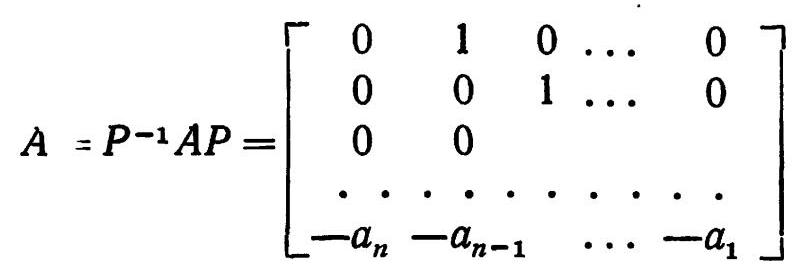
\includegraphics[max width=0.7\textwidth]{images/bo_d547k8bef24c73bgfcg0_442_432_219_802_274_0.jpg}
\end{center}
\hspace*{3em} 

H

\[
\bar{b} = {P}^{-1}b = \left[ \begin{array}{c} 0 \\  0 \\  \vdots \\  1 \end{array} \right]  ,\;\bar{c} = {cP}.
\]

Пользуясь этими координатами, можно легко вычислить переда- точную функцию от входа и к выходу σ,

\[
\bar{c}{\bar{A}}^{-1}\left( z\right) \bar{b} = \frac{\bar{c}\left( z\right) }{\left| A\left( z\right) \right| }.
\]

Здесь \(\left| {A\left( z\right) }\right|\) есть определитель матрицы \(A\left( z\right)\) или \(\bar{A}\left( z\right)  = {zI} - \bar{A}\) , а полином

\[
\bar{c}\left( z\right)  = {\bar{c}}_{n}{z}^{n - 1} + {\bar{c}}_{n - 1}{z}^{n - 2} + \ldots  + {\bar{c}}_{2}z + {\bar{c}}_{1}
\]

имеет своими коэффициентами компоненты вектора \(c = \left( {\overline{{c}_{1}},\overline{{c}_{2}},\ldots }\right. \; \ldots ,{\bar{c}}_{n}).\;\) Это важное вычисление облегчается тем,что

\[
\bar{A}\left( z\right) \left[ \begin{array}{c} 1 \\  z \\  \ldots \\  {z}^{n - 2} \\  {z}^{n - 1} \end{array} \right]   = \left| {A\left( z\right) }\right| \left[ \begin{array}{c} 0 \\  0 \\  \ldots \\  0 \\  1 \end{array} \right]  ,
\]

Так 470

\[
{\bar{A}}^{-1}\left( z\right) \bar{b} = \left[ \begin{array}{c} 1 \\  z \\  \ldots \\  {z}^{n - 1} \end{array} \right]  {\left| \dot{A}\left( z\right) \right| }^{-1}.
\]

Таким образом, для любого заданного действительного полинома \(\bar{c}\left( z\right)\) степени \(\leq  n - 1\) имеется единственный вектор \(c\) ,удовлетво- ряющий соотношению

\[
\overline{c{A}^{-1}}\left( z\right) \bar{b} = \frac{\bar{c}\left( z\right) }{\left| A\left( z\right) \right| }.
\]

Теперь вернемся к координатам х в R", и пусть μ (z)—любой действительный полином степени ≤ \(n - 1\) . Рассмотрим уравнение относительно неизвестного вектора р:

\[
p{A}^{-1}\left( z\right) b = \frac{\mu \left( z\right) }{\left| A\left( z\right) \right| }.
\]

Его можно переписать в виде

\[
\left( {pP}\right) \left( {{P}^{-1}{A}^{-1}\left( z\right) P}\right) \left( {{P}^{-1}b}\right)  = \frac{\mu \left( z\right) }{\left| A\left( z\right) \right| }
\]

относительно \(\left( {pP}\right)\) илн в виде уравнения

\[
\left( {pP}\right) {\bar{A}}^{-1}\left( z\right) \bar{b} = \frac{\mu \left( z\right) }{\left| A\left( z\right) \right| },
\]

которое имеет единственное решение для \(\left( {pP}\right)\) и,таким образом, bektop \(p\) однозначно определен.

Процесс \(\overline{\mathcal{L}}\) и,следовательно,процесс \(\mathcal{L}\left\lbrack  {\text{ нлипара }\left( {A,c}\right) }\right\rbrack\) является вполне наблюдаемым тогда и только тогда, когда

\[
\det \left| {{c}^{\prime },{A}^{\prime }{c}^{\prime },\ldots ,{A}^{\prime n - 1}{c}^{\prime }}\right|  \neq  0.
\]

Corласно лемме 2 теоремы 14 главы 2 процесс 27 является вполне наблюдаемым тогда и только тогда, когда полиномы

\[
\bar{c}\left( z\right)  = {\bar{c}}_{n}{z}^{n - 1} + {c}_{n - 1}{z}^{n - 2} + \ldots  + {c}_{2}z + {c}_{1},
\]

\[
\left| {A\left( z\right) }\right|  = \left| {\bar{A}\left( z\right) }\right|  = \det \left| {{zI} - A}\right|  = {z}^{n} + {a}_{1}{z}^{n - 1} + \ldots  + {a}_{n}
\]

взаимно просты (не имеют общих корней). Таким образом, пара \(\left( {\overline{A},\overline{c}}\right)\) (или система ) только тогда, когда передаточная функция

\[
\bar{c}{\bar{A}}^{-1}\left( z\right) \bar{b} = \frac{\bar{c}\left( z\right) }{\left| A\left( z\right) \right| }
\]

есть дробно-рациональная функция, у которой числитель и зна- менатель взаимно просты. Теперь вернемся к первоначальным координатам \(x\) в \({R}^{n}\) и рассмотрим процесс 8. Вид передаточной функции при переходе от системы Ф к системе 8 (или обратно) не изменяется,

\[
\overset{\text{ ― }}{c}{\overset{\text{ ― }}{A}}^{ - 1}\left( z\right) \overset{\text{ ― }}{b} = \left( {cP}\right) \left( {{P}^{ - 1}{A}^{ - 1}\left( z\right) P}\right) \left( {{P}^{ - 1}b}\right)  = c{A}^{ - 1}\left( z\right) b
\]

и, таким образом, пара (A, c) наблюдаема тогда и только тогда, когда взаимно просты числитель и знаменатель передаточной функции

\[
c{A}^{-1}\left( z\right) b = \frac{\bar{c}\left( z\right) }{\left| A\left( z\right) \right| }.
\]

Вернемся теперь к задаче Лурье о стабилизации систем с не- линейным законом управления. Мы сначала докажем сложную алгебраическую лемму, относящуюся к теории матриц.

Ле мм а. Пусть А—действительная устойчивая п×п-матрица, b и c—действительные п-мерные векторы и τ-неотрицательный скаляр. Предположим, что пара (A, b) вполне управляема и что рачионаяьная компексная фуикция

\[
T\left( z\right)  = \tau  - {2c}{A}^{-1}\left( z\right) b \text{ ≢ } 0
\]

удовлетворяет условию Re \(T\left( {i\omega }\right)  \geq  0\;{при} - \infty  < \omega  < \infty\) . Тогда существуют две действительные симметричные п×п-матрицы

\[
B > 0\;u\;D \geq  0
\]

и п-мерный действительный вектор q такие, что:

1) \({A}^{\prime }B + {B}^{\prime }A =  - q{q}^{\prime } - D\)

2) \({Bb} + {c}^{\prime } + \sqrt{\tau }q = 0\)

3) пара (A, q’) является наблюдаемой.

Доказательство. Заметим, что b и q суть векторы-столбцы, и что с есть вектор-строка, в соответствии с ранее введенными обозначениями. Мы начнем с определения действительного поли- нома

\[
\eta \left( z\right)  = \left| {A\left( z\right) }\right| \left| {A\left( {-z}\right) }\right| \left\{  {\tau  - c{A}^{-1}\left( z\right) b - {b}^{\prime }{A}^{\prime  - 1}\left( {-z}\right) {c}^{\prime }}\right\}  .
\]

Заметим, что степень полинома η(z) равна 2n, так как наивыс- шая степень полиномов — элементов присоединенной матрицы \(\left| {A\left( z\right) }\right| {A}^{-1}\left( z\right)\) ,— есть л — 1, и что старший член η (z) есть (—1)" т z²". [Если \(\tau  = 0\) , то полином η(z) имеет степень <2n. Однако важно лишь, что \(\eta \left( z\right)  \text{ ≢ } 0\) (см. приведенное ниже упражнение).]

Далее, для доказательства необходимо провести анализ струк- туры разложения полинома η (2) на действительные неприводимые (линейные) и квадратичные множители.

Так как \({A}^{\prime }\left( z\right)\) и \(\left| {A\left( z\right) }\right| {A}^{-1}\left( z\right)\) суть действительные полино- миальные матрицы, то \(\eta \left( z\right)\) есть полином с действительными коэффициентами. Так как \(\eta \left( z\right)  = \eta \left( {-z}\right)\) , то \(\eta \left( z\right)\) —четный поли- ном. На мнимой оси (при \(z = {i\omega }\) ) имеем

\[
\operatorname{Re}\eta \left( {i\omega }\right)  = \left| {A\left( {i\omega }\right) }\right| \left| {A\left( {-{i\omega }}\right) }\right| \left\{  {\tau  - 2\operatorname{Re}c{A}^{-1}\left( {i\omega }\right) b}\right\}   \geq  0
\]

при —∞ < ω < ∞, как следует из условий леммы. Таким обра- зом, нули полинома η (z) распределены симметрично относительно действительной и мнимой оси, а нули функции η (i∞) имеют чет- ную кратность [так как Re \(\eta \left( {i\omega }\right)\) не меняет знак на мнимой оси]. Поэтому

\[
\eta \left( z\right)  = \theta \left( z\right) \theta \left( {-z}\right) ,
\]

где 0 (2) есть действительный полином, у которого нет нулей в полуплоскости Re \(z > 0\) . Положим,наконец,

\[
\theta \left( z\right)  = {\theta }_{1}\left( z\right) {\theta }_{2}\left( z\right) ,
\]

где \({\theta }_{1}\left( z\right)\) и \({\theta }_{2}\left( z\right)\) суть действительные полиномы с нулями только в полуплоскости Re \(z < 0\) и только на мнимой оси соответственно. Выберем полином \({\theta }_{2}\left( z\right)\) так, чтобы его старший коэффициент был равен +1. Имеем

\[
\eta \left( z\right)  = {\theta }_{1}\left( z\right) {\theta }_{2}\left( z\right) {\theta }_{1}\left( {-z}\right) {\theta }_{2}\left( {-z}\right) .
\]

Taκ как \({\theta }_{1}\left( {i\omega }\right)\) есть многочлен от ω,не обращающийся в нуль, то

\[
{\theta }_{1}\left( {i\omega }\right) {\theta }_{1}\left( {-{i\omega }}\right)  > {\varepsilon }_{0} > 0\;{\text{ п }\text{ р }\text{ и }}\; - \infty  < \omega  < \infty .
\]

Пусть а—такое действительное положительное число, что

\[
{\alpha }^{2} \leq  {\varepsilon }_{0}\;n\;{\alpha }^{2} \neq  {\theta }_{1}\left( {\lambda }_{i}\right) {\theta }_{1}\left( {-{\lambda }_{i}}\right) ,
\]

где \({\lambda }_{1},{\lambda }_{2},\ldots ,{\lambda }_{n}\) cyть характеристические числа матрицы \(A\) . Если \({\theta }_{1}\left( z\right)  -\) константа, то полагаем а = 0.

Пользуясь свойством управляемости пары (A, b), определим действительный вектор \(g\) с помощью соотношения

\[
{g}^{\prime }{A}^{-1}\left( z\right) b = \frac{\alpha {\theta }_{2}\left( z\right) }{\left| A\left( z\right) \right| }.
\]

Это возможно, так как степень полинома б, (2) меньше л, если полином \({\theta }_{1}\left( z\right)\) не является константой и α ≠ 0. Нужная нам сим- метричная матрица \(D\) задается соотношением

\[
D = g{g}^{\prime }\text{ . }
\]

рассмотрим действительный четный полином

\[
\Gamma \left( z\right)  = {\theta }_{2}\left( z\right) {\theta }_{2}\left( {-z}\right) \left\lbrack  {{\theta }_{1}\left( z\right) {\theta }_{1}\left( {-z}\right)  - {\alpha }^{2}}\right\rbrack  .
\]

Так kak

\[
{\theta }_{2}\left( {i\omega }\right) {\theta }_{2}\left( {-{i\omega }}\right)  \geq  0
\]

и

\[
{\theta }_{1}\left( {i\omega }\right) {\theta }_{1}\left( {-{i\omega }}\right)  > {\varepsilon }_{0} \geq  {\alpha }^{2},
\]

то \(\Gamma \left( {i\omega }\right)  \geq  0\) для всех действительных ω. Кроме того, полином \(\Gamma \left( z\right)\) взаимно прост с полиномом \(\left| {A\left( z\right) }\right| \left| {A\left( {-z}\right) }\right|\) ,так как нули полинома \(\Gamma \left( z\right)\) не равны ни одному из чисел \(\pm  {\lambda }_{1}, \pm  {\lambda }_{2},\ldots\) ,или \(\pm  {\lambda }_{n}\) . Так как Г(2) есть действительный четный полином и \(\operatorname{Re}\Gamma \left( {i\omega }\right)  \geq  0\) ,то существует действительный полином v (z) с нулями только в полуплоскости Re \(z \leq  0\) ,и такой,что

\[
\Gamma \left( z\right)  = v\left( z\right) v\left( {-z}\right) .
\]

Так как главный член полинома Г(z) тот же, что и у полинома \(\eta \left( z\right)\) , a именно \({\left( -1\right) }^{n}\tau {z}^{2n}\) ,то в качестве v(z) можно взять поли- ном с главным членом \(\sqrt{\tau }{z}^{n}\) .

Теперь разделим v (z) на \(\left| {A\left( z\right) }\right|\) . Частное есть \(\sqrt{\tau }\) , a остаток мы обозначим через - μ (2)

\[
\frac{v\left( z\right) }{\left| A\left( z\right) \right| } =  - \frac{\mu \left( z\right) }{\left| A\left( z\right) \right| } + \sqrt{\tau }.
\]

Здесь и (2) есть действительный полином степени меньшей, чем л. Ясно, что μ(z) ≢ 0, ибо в этом случае

\[
v\left( z\right)  = \sqrt{\tau }\left| {A\left( z\right) }\right| \;\text{ и }\;\Gamma \left( z\right)  = \tau \left| {A\left( z\right) }\right|  \cdot  \left| {A\left( {-z}\right) }\right| ,
\]

что противоречит тому факту, что полином Г(z) взаимно прост с полиномом \(\left| {A\left( z\right) }\right| \left| {A\left( {-z}\right) }\right|\) . [Если \(\tau  = 0\) , ro \(v\left( z\right)  =  - \mu \left( z\right)  \text{ ≢ } 0\) .]

Определим вектор \(q\) cootnoшением

\[
{q}^{\prime }{A}^{-1}\left( z\right) b = \frac{-\mu \left( z\right) }{\left| A\left( z\right) \right| }.
\]

Поскольку полиномы μ (2) и | A (2) | взаимно просты, то из теории наблюдаемости следует, что пара \(\left( {A,{q}^{\prime }}\right)\) является вполне наблю- даемой. Зададим положительно определенную матрицу В> 0 соот- ношением

\[
{A}^{\prime }B + {B}^{\prime }A =  - q{q}^{\prime } - D,
\]

HJIM

\[
B = {\int }_{0}^{\infty }{e}^{{A}^{\prime }t}\left\{  {q{q}^{\prime } + D}\right\}  {e}^{At}{dt}
\]

Покажем теперь, что

\[
{Bb} + {c}^{\prime } + \sqrt{\tau }q = 0.
\]

Для этого заметим, что

\[
v\left( z\right) v\left( {-z}\right)  = \Gamma \left( z\right)  = \eta \left( z\right)  - {\alpha }^{2}{\theta }_{2}\left( z\right) {\theta }_{2}\left( {-z}\right) .
\]

Делением обеих частей последнего равенства на \(\left| {A\left( z\right) }\right|  \cdot   \mid  A\left( {-z}\right)\) получим

\[
\left\lbrack  {\frac{-\mu \left( z\right) }{\left| A\left( z\right) \right| } + \sqrt{\tau }}\right\rbrack  \left\lbrack  {\frac{-\mu \left( {-z}\right) }{\left| A\left( -z\right) \right| } + \sqrt{\tau }}\right\rbrack   =
\]

\[
= \left\{  {\tau  - c{A}^{-1}\left( z\right) b - {b}^{\prime }{A}^{\prime  - 1}\left( {-z}\right) {c}^{\prime }}\right\}   - {b}^{\prime }{A}^{\prime  - 1}\left( z\right) g{g}^{\prime }{A}^{-1}\left( {-z}\right) b.
\]

Заменяя — \(\mu \left( z\right) /\left| {A\left( z\right) }\right|\) на \({q}^{\prime }{A}^{-1}\left( z\right) b\) и полагая \(z = {i\omega }\) ,после не- которых упрощений получим

\[
c\left\{  {{A}^{-1}\left( {i\omega }\right)  + {A}^{-1}\left( {-{i\omega }}\right) }\right\}  b + \sqrt{\tau }{q}^{\prime }\left\{  {{A}^{-1}\left( {i\omega }\right)  + {A}^{-1}\left( {-{i\omega }}\right) }\right\}  b =
\]

\[
= {b}^{\prime }{A}^{\prime  - 1}\left( {i\omega }\right) \left\{  {-q{q}^{\prime } - g{g}^{\prime }}\right\}  {A}^{-1}\left( {-{i\omega }}\right) b.
\]

Учитывая соотношение

\[
{A}^{\prime }B + {B}^{\prime }A =  - q{q}^{\prime } - g{g}^{\prime }
\]

и используя формулы

\[
A = {zI} - A\left( z\right) ,\;{A}^{-1}\left( z\right) A = A{A}^{-1}\left( z\right)  = z{A}^{-1}\left( z\right)  - I,
\]

HAMACM, ЧТО

\[
c + \sqrt{\tau }{q}^{\prime })\left\{  {{A}^{-1}\left( {i\omega }\right)  + {A}^{-1}\left( {-{i\omega }}\right) }\right\}  b =  - {b}^{\prime }B\left\{  {{A}^{-1}\left( {i\omega }\right)  + {A}^{-1}\left( {-{i\omega }}\right) }\right\}  b.
\]

Takhh oópa3OM,

\[
\operatorname{Re}\left( {{b}^{\prime }B + c + \sqrt{\tau }{q}^{\prime }}\right) {A}^{-1}\left( {i\omega }\right)  = 0.
\]

Но \({A}^{-1}\left( 0\right)  =  - {A}^{-1}\) есть действительная и неособая матрица, так что

\[
{b}^{\prime }B + c + \sqrt{\tau }{q}^{\prime } = 0.
\]

Поэтому

\[
{Bb} + {c}^{\prime } + \sqrt{\tau q} = 0,
\]

что и требовалось. Лемма доказана.

Мы приведем краткое следствие, представляющее собой неко- торую модификацию доказанной леммы.

Следствие. Пусть А—действительная устойчивая п×п-мат- рица, а b и с действительные n-мерные векторы. Если

\[
T\left( {i\omega }\right)  \geq  0\;{\pi }_{\mathrm{{PH}}} - \infty  < \omega  < \infty ,
\]

mo

\[
\operatorname{Re}T\left( z\right)  \geq  0\;\text{ при }\operatorname{Re}z \geq  0.
\]

Доказательство. Заметим, что \(T\left( z\right)  = \tau  - {2c}{A}^{-1}\left( z\right) b\) есть комплекснозначная аналитическая функция без особенностей в по- луплоскости Re \(z \geq  0\) ,так что Re \(T\left( z\right)\) есть гармоническая функ- ция в правой полуплоскости. Но

\[
\mathop{\lim }\limits_{{\left| z\right|  \rightarrow  \infty }}T\left( z\right)  = \tau  \geq  0,\;\operatorname{ec\text{ л }\text{ и }}\;\operatorname{Re}z \geq  0
\]

и, следовательно, функция Re \(T\left( z\right)\) неотрицательна, если z лежит в правой полуплоскости и имеет достаточно большой модуль. Таким образом,

\[
\operatorname{Re}T\left( {i\omega }\right)  \geq  0\;{\text{ п }\text{ р }\text{ и }}\; - \infty  < \omega  < \infty .
\]

Если теперь Re \(T\left( {z}_{0}\right)  < 0\) в некоторой точке \({z}_{0}\) из правой полу- плоскости, то гармоническая функция — Re \(T\left( z\right)\) где-то в области \(\operatorname{Re}z > 0\) должна иметь максимум. Но это противоречит принципу максимума для гармонических функций. Следовательно,

\[
\operatorname{Re}T\left( z\right)  \geq  0\;\text{ при }\operatorname{Re}z \geq  0,
\]

что и требуется. Следствие доказано.

Следствие показывает, что предположение леммы относительно функции \(T\left( z\right)\) можно заменить условием

\[
\operatorname{Re}T\left( z\right)  \geq  0,\;\operatorname{ec\text{ л }\text{ и }}\operatorname{Re}z \geq  0,
\]

которое выглядит естественнее и при этом не ограничивает об- щности утверждения леммы. Условие \(T\left( z\right)  \text{ ≢ } 0\) эквивалентно тре- бованию τ+|c|>0 (см. упражнения). Такие функции иногда на- зывают положительными и класс таких функций изучается в тео- рии аналитических функций комплексного переменного. В последней формулировке лемма напоминает критерий устойчивости для про- цессов с линейным законом управления. Эта лемма нам понадо- билась для доказательства следующей теоремы.

Теорема 10. Рассмотрим процесс в R":

(八)
\[
\dot{x} = {Ax} + {bu}\left( \sigma \right) ,\;\sigma  = {cx}
\]

с законом управления и (σ) из класса U, где А есть действитель- ная устойчивая матрица, b и c-действительные векторы, а пара \(\left( {A,b}\right)\) вполне управляема. Предположим, что существуют неотри- цательные действительные числа а и β, где α + β > 0 такие, что рациональная комплексная функция

\[
T\left( z\right)  =  - \left( {\alpha  + {\beta z}}\right) c{A}^{-1}\left( z\right) b
\]

yòoèremeopaem ycnoeuro

\[
\operatorname{Re}T\left( {i\omega }\right)  \geq  0\;\text{ при } - \infty  < \omega  < \infty .
\]

Тогда начало координат есть устойчивая критическая точка про- цесса Л для каждого и (σ) из U. Если, кроме того, а > 0, то процесс Л является глобально асимптотически устойчивым и, сле- довательно, абсолютно устойчивым.

Доказательство. Пользуясь равенством zI=A(z)+A, получим

\[
T\left( z\right)  =  - {\beta cb} - 2\left( \frac{{\beta cA} + {\alpha c}}{.2}\right) {A}^{-1}\left( z\right) b.
\]

TaK Kak lim \({A}^{-1}\left( z\right)  = 0\) и \(\operatorname{Re}T\left( {i\omega }\right)  \geq  0\) , ro \(- {\beta cb} \geq  0\) . Заметим, что \(T\left( z\right)  \text{ ≢ } 0\) , иначе выполнялось бы равенство с \({A}^{-1}\left( z\right) b \equiv  0\) , которое означает (см. упражнение ниже), что c=0. Но мы исклю- чаем из рассмотрения этот случай, ибо при се 0 теорема триви- альна. Применим лемму, полагая

\[
\tau  =  - {\beta cb}\;\text{ и }\;k = \frac{{\beta cA} + {\alpha c}}{2}.
\]

Corласно лемме существуют симметричные матрицы \(B > 0\) и \(D \geq  0\) и вектор \(q\) ,такие,что

\[
{A}^{\prime }B + {B}^{\prime }A =  - q{q}^{\prime } - D,\;{Bb} + {\left( \frac{{\beta cA} + {\alpha c}}{2}\right) }^{\prime } + \sqrt{\tau }q = 0.
\]

Определим действительную функцию в \({R}^{n + 1}\) :

\[
V\left( {x,\sigma }\right)  = {x}^{\prime }{Bx} + \beta {\int }_{0}^{\sigma }u\left( s\right) {ds}
\]

Ясно,что \(V\left( {x,\sigma }\right)  \geq  0\) ,причем \(V\left( {x,\sigma }\right)  > 0\) при \(x \neq  0\) н

\[
\mathop{\lim }\limits_{{\left| x\right|  \rightarrow  \infty }}V\left( {x,\sigma }\right)  = \infty .
\]

Вычислим производную от функции \(V\) вдоль произвольного ре- шения \(x\left( t\right) ,\sigma \left( t\right)  = {cx}\left( t\right)\) системы

\[
\dot{x} = {Ax} + {bu}\left( \sigma \right) ,\;\dot{\sigma } = {cAx} + {cbu}\left( \sigma \right)
\]

в \({R}^{n + 1}\) , cootветствующего фнкснрованному управлению \(u\left( \sigma \right)  \in  \mathcal{U}\) :

\[
\dot{V} = {x}^{\prime }B\left( {{Ax} + {bu}\left( \sigma \right) }\right)  + \left( {{x}^{\prime }{A}^{\prime } + u\left( \sigma \right) {b}^{\prime }}\right) {Bx} + {\beta u}\left( \sigma \right) \left( {{cAx} + {cbu}\left( \sigma \right) }\right) ,
\]

откуда

\[
- \dot{V} =  - {x}^{\prime }\left( {{BA} + {A}^{\prime }B}\right) x - \left( {2{b}^{\prime }B + {\beta cA}}\right) {xu}\left( \sigma \right)  - {\beta cb}{u}^{2}\left( \sigma \right) ,
\]

WIM

\[
- \dot{V} = {x}^{\prime }{Dx} + {x}^{\prime }q{q}^{\prime }x + 2{\left( -Bb - \frac{\beta {A}^{\prime }{c}^{\prime } + \alpha {c}^{\prime }}{2}\right) }^{\prime }{xu}\left( \sigma \right)  + {\alpha cxu}\left( \sigma \right)  + \tau {u}^{2}\left( \sigma \right) .
\]

Из последнего соотношения следует, что

\[
- \dot{V} = {x}^{\prime }{Dx} + {\left( \sqrt{\tau }u\left( \sigma \right)  + {q}^{\prime }x\right) }^{2} + {\alpha \sigma u}\left( \sigma \right)  \geq  0.
\]

Пусть \({x}_{0},{\sigma }_{0} = c{x}_{0}\) есть начальное состояние системы. Тогда сот- betchbouse penemae \(x\left( t\right)\) удовлетворяет условию

\[
{x}^{\prime }{Bx} \leq  V\left( {{x}_{0},c{x}_{0}}\right) .
\]

Тем самым решение х (н) определено для "всех t из интервала \(0 \leq  t < \infty\) ,и начало координат является устойчивой критической точкой.

Предположим, что α > 0. Если решение x(t) не приближается к началу координат, то оно должно стремиться при t+ 30 к не- которой точке \(x \in  {R}^{n}\) ,так чтобы

\[
\mathop{\lim }\limits_{{t \rightarrow  \infty }}V\left( {x\left( t\right) ,{cx}\left( t\right) }\right)  = V\left( {\bar{x},c\bar{x}}\right)  > 0.
\]

Но решение \(\left( {\bar{x}\left( t\right) ,\overline{\sigma }\left( t\right) }\right)\) , начинающееся в точке ( \(\bar{x},c\bar{x}\) ), удовлет- воряет неравенству

\[
V\left( {\bar{x}\left( t\right) ,c\bar{x}\left( t\right) }\right)  < V\left( {\bar{x},c\bar{x}}\right) ,
\]

для некоторого \(t > 0\) ,и по непрерывности \(V\left( {x\left( t\right) ,{cx}\left( t\right) }\right)  < V\left( {\bar{x},c\bar{x}}\right)\) , если только \(\sigma \left( t\right)  \text{ ≢ } 0\) . Но в этом исключительном случае решение \(\bar{x}\left( t\right)\) удовлетворяет уравнению \(\dot{x} = {Ax}\) или \(\bar{x}\left( t\right)  = {e}^{At}\bar{x}\mathbf{u} - \dot{V} = {x}^{\prime }{Dx} + \; + {\left( {q}^{\prime }x\right) }^{2} = 0\) . Но тогда \({q}^{\prime }{e}^{At}\overline{x} \equiv  0\) , orкуда в силу условия наблю- даемости пары \(\left( {A,{q}^{\prime }}\right)\) следует, что \(\bar{x} = 0\) ,что является противо- речием. Итак,

\[
\mathop{\lim }\limits_{{t \rightarrow  \infty }}x\left( t\right)  = 0,
\]

и процесс Л является абсолютно устойчивым. Теорема доказана.

Следующая теорема распространяет задачу Лурье на нелиней- ные процессы с нелинейным законом управления и (о) из И. Мы докажем, что алгебраические условия теоремы 10 гарантируют асимптотическую устойчивость системы относительно начала коор- динат при любом \(u\left( \sigma \right)  \in  \mathcal{U}\) . Конечно, это утверждение для нели- нейного процесса относится лишь к некоторой окрестности начала координат.

Теорема 11. Рассмотрим процесс в R":

(∑
\[
{}^{(}2)
\]

\[
\dot{x} = f\left( {x,u}\right)  = {Ax} + {bu} + o\left( {x,u}\right) \;\kappa \text{ nacca }{C}^{1}
\]

с заданной обратной связью

\[
\sigma  = \sigma \left( x\right)  = {cx} + o\left( x\right) \kappa \overset{ }{\kappa }\overset{ }{c}{ca}\;{C}^{1}
\]

и законом управления и (σ) из U. Предположим, что А есть дей- ствительная устойчивая матрица, b и c —действительные векторы, причем пара (A, b) вполне управляема. Предположим далее, что существуют действительные числа

\[
\alpha  > 0,\beta  > 0\;{ma\kappa ue},{\iota mo}\;\tau  =  - {\beta cb} > 0
\]

u umo paquonarbhar фулкция

\[
T\left( z\right)  =  - \left( {\alpha  + {\beta z}}\right) c{A}^{-1}\left( z\right) b
\]

yòoēremeopяem yсловию

\[
\operatorname{Re}T\left( {i\omega }\right)  \geq  0\;\text{ при }\; - \infty  < \omega  < \infty .
\]

Тогда процесс Σ асимптотически устойчив относительно начала координат для каждого \(u\left( \sigma \right)  \in  \mathcal{U}\) ,где и'(0) > 0.

Доказательство. Пусть о \(\left( {x,u}\right)\) есть величина высшего порядка малости по сравнению с (|x|+|u|). Положим

\[
A = \frac{\partial f}{\partial x}\left( {0,0}\right) ,\;b = \frac{\partial {f}_{i}}{\partial u}\left( {0,0}\right) ,\;c = \frac{\partial \sigma }{\partial x}\left( 0\right) .
\]

Пусть матрицы B >0, D ≥0 и вектор \(q \neq  0\) , получены так же, как и в теореме 10. Фиксируем закон управления и (о) ∈ И и оп- ределим действительную функцию в R\textasciicircum +1 по формуле

\[
V\left( {x,\sigma }\right)  = {x}^{\prime }{Bx} + \beta {\int }_{0}^{\sigma }u\left( s\right) {ds}.
\]

Ясно, что \(V\left( {x,\sigma }\right)  > 0\) всюду, кроме х=0=0. Выберем в качестве начального состояния точку \({x}_{0} \neq  0\) в \({R}^{n}\) ,и пусть \(x\left( t\right)\) -сответ- ствующее решение уравнения

\[
\dot{x} = f\left( {x,u\left( {\sigma \left( x\right) }\right) }\right) .
\]

Полагая σ(t)=σ(x(t)) и вычисляя производную от функции \(V\left( t\right)  = V\left( {x\left( t\right) ,\sigma \left( {x\left( t\right) }\right) }\right)\) ,получаем

\[
- \dot{V} = {x}^{\prime }{Dx} + {\left( \sqrt{\tau }u + {q}^{\prime }x\right) }^{2} + \alpha \left( {\sigma  - o\left( x\right) }\right) u + {uo}\left( {x,u}\right)  + {xo}\left( {x,u}\right) .
\]

Однако, поскольку матрица D не является положительно опре- деленной, то очевидная оценка по Ляпунову может и не проходить для произвольного управления \(u\left( t\right)  \in  \mathcal{U}\) .

Поэтому положим \(u\left( \sigma \right)  = {u}_{1}\sigma  + o\left( \sigma \right)\) ,где \({u}_{1} = {u}^{\prime }\left( 0\right)  > 0\) . Тогда, по теореме 10, линейный процесс

(Л)
\[
\dot{x} = {Ax} + {bu}\left( \sigma \right) ,\;\sigma  = {cx}
\]

будет аснмптотически устойчивым при линейном законе управле- ния \(u = {u}_{1}\sigma\) . Однако \(\mathcal{N}\) в точности совпадает с линеаризацией не- линейного процесса( )

\[
\dot{x} = f\left( {x,u\left( {\sigma \left( x\right) }\right) }\right)
\]

для заданного закона управления \(u\left( \sigma \right)  = {u}_{1}\sigma  + o\left( \sigma \right)\) . Следовательно, 5 — асимптотически устойчивый процесс в окрестности начала координат, что и требовалось доказать.

В качестве последнего вопроса теории устойчивости мы рас- смотрим вопрос о корректности задачи оптимального управления. Является ли задача оптимального управления хорошо поставлен- ной в том смысле, что малые изменения данных задачи порождают лишь малые изменения критерия оптимальности?

Рассмотрим задачу управления в R":

\[
P = \left\{  {\mathcal{S},C,{X}_{0},{X}_{1},\Omega }\right\}
\]

для процесса(\$)

\[
\dot{x} = A\left( x\right)  + B\left( x\right) u
\]

с критерием качества

\[
C\left( u\right)  = {\int }_{0}^{{t}_{1}}\left\lbrack  {{A}^{0}\left( x\right)  + {B}^{0}\left( x\right) u}\right\rbrack  {dt},
\]

и коэффициентами \(A\left( x\right) ,B\left( x\right) ,{A}^{0}\left( x\right) ,{B}^{0}\left( x\right)\) класса \({C}^{1}\) в \({R}^{n}\) . Управления суть измеримые функции \(u\left( t\right)\) , onределенные на раз- личных подынтервалах 0 0 ≤0 кс, 1 заданного конечного интервала \(0 \leq  t \leq  T\) ,причем и (t) ⊂ Ω, где Ω—компактное выпуклое ограни- чивающее множество в R". Мы пытаемся перевести некоторую точку компактного множества Х, начальных состояний в точку компактного целевого множества Х1 в пространстве R" при опти- мальном (минимальном) значении критерия качества C(u).

Мы скажем, что другая такая задача управления

\[
\widehat{P} = \{ \widehat{S},\widehat{C},{\widehat{X}}_{0},{\widehat{X}}_{1},\widehat{\Omega }\} ,
\]

лежит на расстоянии, не превосходящем δ or \(P\) , если

\(\left| {A\left( x\right)  - \widehat{A}\left( x\right) }\right|  + \left| {B\left( x\right)  - \widehat{B}\left( x\right) }\right|  + \left| {{A}^{0}\left( x\right)  - {\widehat{A}}^{0}\left( x\right) }\right|  + \left| {{B}^{0}\left( x\right)  - {\widehat{B}}^{0}\left( x\right) }\right|  < \delta ,\) когда \(\left| x\right|  < \frac{1}{\delta }\) ,и

\[
\operatorname{dist}\left( {{X}_{0},{\widehat{X}}_{0}}\right)  + \operatorname{dist}\left( {{X}_{1},{\widehat{X}}_{1}}\right)  + \operatorname{dist}\left( {\Omega ,\widehat{\Omega }}\right)  < \delta
\]

(мы пользуемся принадлежащим Хаусдорфу определением рассто- яния между непустыми компактными подмножествами пространств \({R}^{n}\) и \({R}^{m}\) ). Расстояние между задачами \(P\) и \(\widehat{P}\) мы определим как точную нижнюю грань всех таких δ >0. Тем самым, мы трактуем множество 7 всех таких задач управления как метрическое пространство.

Теорема 12. Рассмотрим задачу управления Р в простран- стве P, заданную в R" системой

(\$)
\[
\dot{x} = A\left( x\right)  + B\left( x\right) u
\]

с крциерцем качесмеа

\[
C\left( u\right)  = {\int }_{0}^{{t}_{1}}\left\lbrack  {{A}^{0}\left( x\right)  + {B}^{0}\left( x\right) u}\right\rbrack  {dt}
\]

\(c\) коэффициентами \(A\left( x\right) ,{A}^{0}\left( x\right) ,B\left( x\right) ,{B}^{0}\left( x\right)\) класса \({C}^{1}B{R}^{n}\) ,из- меримыми управлениями и (t)С Ω, определенными на различных интервалах 0 ≤ t ≤ t, ≤ T и компактным выпуклым ограничи- вающим множеством \(\Omega  \subset  {R}^{m}\) .

Начальную точку х, ес пыльно по оптимальной траектории перевести в целевую точку \({x}_{1} = 0\) .

Предположим, что:

(a) существует равномерная оценка |x(t)|<β для всех траек- торий процесса S, начинающихся в точке x(0)=x, и соответст- вующих управлениям и (t) ⊂ Ω на интервале 0 ≤ t ≤ T + 1;

(b) существует допустимая траектория системы \$, переводя- щая точку х, в точку х, перигну три системы \$, переводя- лению \({u}_{0}\left( t\right) \left( {0 \leq  t \leq  {t}_{1}}\right)\) , umo \(C\left( {u}_{0}\right)  < C\left( u\right) \partial {\lambda A}\) всех и (t) \((0 \leq  t \leq  \tau\) ; \(T \leq  \tau  \leq  T + 1)\) co значениями в Ω;

(c) rank \(\left\lbrack  {B,{AB},{A}^{2}B,\ldots ,{A}^{n - 1}B}\right\rbrack   = n,e\partial {eA}\left( 0\right)  = 0,A = \frac{\partial A}{\partial x}\left( 0\right)\) , \(B = B\left( 0\right) ;c\)

(d) \(\Omega\) codepжum точку u =0 внутри себя.

Тогда существует окрестность N задачи P в пространстве P такая, что каждая задача р€Ж обладает оптимальным управ- лением \({\widehat{u}}^{ * }\left( t\right)\) , onpeделенным на интервале 0 ≤ \(t \leq  {t}^{ * } \leq  T\) , a onmu- мальное значение критерия качества C (и*) стремится к C (и*), \({\kappa o2a}\widehat{P}\) cmpémum \(\kappa P\) .

Доказательство. Первые два условия предполагают су- ществование оптимального управления \({u}^{ * }\left( t\right)  \subset  \Omega\) для задачи P, определенного на интервале 0 ≤ t ≤ t*. Кроме того, \(C\left( {u}^{ * }\right)  < \inf C\left( u\right)\) для всех и (t) с Ω (0 ≤ t ≤ τ ; T < τ ≤ τ < T + 1 ).

Пусть теперь задача Р лежит в некоторой достаточно малой окрестности N задачи Р в метрическом пространстве Ф. Общеиз- вестные оценки показывают, что имеется равномерная граница для всех траекторий процесса \$, соответствующих управлениям й (н)сл \(\left( {0 \leq  t \leq  T + 1}\right)\) . Таким образом, если точки множества А, оможно пе- ревести в точки множества д \({\widehat{X}}_{1}\) с помощью управлений из Ω, O пре- деленных на интервалах 0 ≤ t ≤ c, t < c > 0, то задача P обладает оптимальным управлением \({\widehat{u}}^{ * }\left( t\right) \left( {0 \leq  t \leq  {t}^{ * };{t}^{ * } \leq  T}\right)\) .

Пусть управление \({u}^{ * }\left( t\right)\) , onpeделенное на интервале 0 ≤ \(t \leq  {t}^{ * }\) , переводит точку х, оптимально в х, =0 вдоль траектории систе- мы у. Пусть управление \({\widehat{u}}_{1}\left( t\right)\) -ближайшая к \({u}^{ * }\left( t\right)\) точка в \(\widehat{\Omega }\) , и пусть точка \({\widehat{x}}_{0} \in  {X}_{0}\) близка к \({x}_{0}\) . Тогда управление \({\widehat{u}}_{1}\left( t\right)\) перево- дит точку \({\widehat{x}}_{0}\) в некоторую точку х, из некоторой окрестности на- чала координат, вдоль траектории процесса Ф. При предположе- ниях (c) и (d) точку и, можно перевести в любую точку в окрест- ности начала координат малыми управлениями из \(\Omega  \cap  \widehat{\Omega }\) вдоль траекторий процесса £. С помощью методов приближения, исполь- зуемых в локальной теории управляемости, мы находим, что точку \({\widehat{x}}_{1}\) в течение короткого промежутка времени можно перевести в множество \({\widehat{X}}_{1}\) вдоль траектории процесса Ф. Поэтому для каждой задачи \(\widehat{P}\) из достаточно малой окрестности № существует оптималь- ное управление \({\widehat{u}}^{ * }\left( t\right)\) , onpeдeленное на интервале 0 \(\leq  t \leq  {t}^{ * }\left( {{t}^{ * } < T}\right)\) .

Пользуясь изложенной конструкцией, можно показать, что для любого наперед заданного ε> 0 существует столь малая окрест- HOCTb \({\mathcal{N}}_{1} \subset  \mathcal{N}\) , что \(\widehat{C}\left( {\widehat{u}}^{ * }\right)  < C\left( {u}^{ * }\right)  + \varepsilon\) . Tenepb предположим, что \(\widehat{C}\left( {\widehat{u}}^{ * }\right)  < C\left( {u}^{ * }\right)  - \varepsilon\) для некоторого \(\widehat{P} \subset  {\mathcal{N}}_{1}\) ,независимо от того,как мала окрестность \({\mathcal{N}}_{1}\) ,выбираемая для задачи P. Тогда, пользуясь управлением \(\widetilde{u}\left( t\right)  \subset  \Omega\) ,ближайшим \(\kappa {\widehat{u}}^{ * }\left( t\right)\) ,точку \({x}_{0}\) можно пере- вести в окрестность точки \({x}_{1} = 0\) за время 0 \(\leq  t \leq  {\widehat{t}}^{ * },{\widehat{t}}^{ * } \leq  T\) , u отсюда перевести точно в \({x}_{1} = 0\) некоторым управлением \(\widetilde{\widetilde{u}}\) , ompe- деленным на отрезке 0 ≤ t ≤ T + 1 с критерием качества C \(\left( \widetilde{\widetilde{u}}\right)  < \; < C\left( {u}^{ * }\right)  - \frac{\varepsilon }{2}\) . Но это противоречит условию (b) и, таким образом, \(C\left( \widehat{{u}^{ * }}\right)  \geq  C\left( {u}^{ * }\right)  - \varepsilon\) всякий раз, когда окрестность \({\mathcal{N}}_{1}\) достаточно мала. Поэтому функция \(\widehat{C}\left( \widehat{{u}^{ * }}\right)\) ,являясь одновременно функцией от \(\widehat{P} \in  \mathcal{P}\) ,непрерывна по \(\widehat{P}\) в точке P. Теорема доказана.

Cледствие 1. Пусть Р(*) — последовательность задач управ- ления из \(\mathcal{N} \subset  \mathcal{P}\) и пусть

\[
\mathop{\lim }\limits_{{k \rightarrow  \infty }}{P}^{\left( k\right) } = P
\]

Тогда существует подпоследовательность — \({t}_{\left( {k}_{i}\right) }^{ * } \rightarrow  {t}^{ * },\)

\[
\mathop{\lim }\limits_{{i \rightarrow  \infty }}{u}_{\left( {k}_{i}\right) }^{ * }\left( t\right)  = {u}^{ * }\left( t\right) \operatorname{cna}{\delta o}
\]

\(u\)

\[
\mathop{\lim }\limits_{{i \rightarrow  \infty }}{x}_{\left( {k}_{i}\right) }^{ * }\left( t\right)  = {x}^{ * }\left( t\right) \text{ paвиомерно }
\]

на каждом компактном подынтервале отрезка 0 месяка 0 местна. \({u}^{ * }\left( t\right)  \subset  \Omega \left( {0 \leq  t \leq  {t}^{ * }}\right)\) ecm bonnuмальное управление для задачи P, \({x}^{ * }\left( t\right)  -\) coomвemcтвующее решение.

Доказательство. Так как все б н лежат на компактном интервале, подпоследовательность \({t}_{\left( {k}_{i}\right) }^{ * }\) сходится к некоторой точке \({t}^{ * } \leq  T\) . Так как все \({u}_{\left( {k}_{i}\right) }^{ * }\left( t\right)  \subset  {\Omega }_{\left( {k}_{i}\right) }\) и \({\Omega }_{\left( {k}_{i}\right) } \rightarrow  \Omega\) , to функции \({u}_{\left( {k}_{i}\right) }^{ * }\left( t\right)\) равномерно ограничены на компактном интервале времени 0≤/t ≤ \(\leq  \overrightarrow{t} < {t}^{ * }\) и на нем подпоследовательность слабо сходится. Заме- тим, что все икну (н определены на интервале 0 ≤ t ≤ t для боль- ших \({k}_{i}\) и мы сохраняем за соответствующей подпоследовательностью обозначение и «и) (t). Обозначим через и « (t) ее слабый предел. Ясно, что \({u}^{ * }\left( t\right)  \subset  \Omega\) (почти всюду), tak как в силу предположения о том, что \({u}_{\left( {k}_{i}\right) }^{ * } \subset  {\Omega }_{\left( {k}_{i}\right) }\) и \({\Omega }_{\left( {k}_{i}\right) } \rightarrow  \Omega\) ,точка \({u}^{ * }\left( t\right)\) не может лежать снаружи какой-либо из счетного числа гиперплоскостей, определяющих об- ласть \(\Omega\) в течение промежутка времени ненулевой длительности. Соответствующие решения \({x}_{\left( {k}_{i}\right) }^{ * }\left( t\right)\) равномерно ограничены с равно- мерно ограниченными производными, и таким образом, подпосле- довательность \({x}_{\left( {k}_{i}\right) }\) (пока еще занумерованная индексами к) сходится равномерно на каждом подынтервале 0≤ t ≤ i; i < t* к некоторой предельной функции \({x}^{ * }\left( t\right)\) .

Пользуясь методами доказательства теорем существования главы 4, мы находим, что и * (н) (0 ≤ t ≤ t*) является допустимым управлением для процесса \(\mathcal{L}\) ,переводящим точку х,в точку \({x}_{1}\) в точку \({x}_{1} = 0\) вдоль решения \({x}^{ * }\left( t\right)\) . Аналогично, \({C}_{\left( {k}_{i}\right) }\left( {u}_{\left( {k}_{i}\right) }^{ * }\right)  \rightarrow  C\left( {u}^{ * }\right)\) и, checloga- тельно, \({u}^{ * }\left( t\right)\) есть оптимальное управление для процесса \$. След- ствие доказано.

Cледствие 2. Рассмотрим задачу управления Р в простран- стве P, соответствующую системе(\$)

\[
\dot{x} = A\left( x\right)  + B\left( x\right) u\;e\;{R}^{n},
\]

с критерием качества

\[
C\left( u\right)  = {t}_{1}.
\]

В условиях теоремы существует такая окрестность N задачи Р в пространстве Ф, что каждая задача управления РЕ \$N имеет оптимальное значение критерия качества i* < T, причем i* стре- мится \(\kappa {t}^{ * }\) ,когда \(\widehat{P}\) cmpемится \({\kappa P}\) .

\section*{Упражнения}

1. Рассмотрим позиционное управление вращающимся твердым телом:

\[
{I}_{1}{\dot{\omega }}_{1} = \left( {{I}_{2} - {I}_{3}}\right) {\omega }_{2}{\omega }_{3} + {u}_{1}\left( t\right) ,
\]

\[
{I}_{2}{\dot{\omega }}_{2} = \left( {{I}_{3} - {I}_{1}}\right) {\omega }_{3}{\omega }_{1} + {u}_{2}\left( t\right) ,
\]

\[
{I}_{3}{\dot{\omega }}_{3} = \left( {{I}_{1} - {I}_{2}}\right) {\omega }_{1}{\omega }_{2} + {u}_{3}\left( t\right) ,
\]

где \({I}_{1},{I}_{2},{I}_{3}\) есть главные моменты инерции, а \({\omega }_{1},{\omega }_{2},{\omega }_{3}\) - соответствующие компоненты угловой скорости. Построить функцию Ляпунова и доказать, что система может быть переведена из любого заданного начального состояния в начало координат посредством управлений, удовлетворяющих ограничению \(\left| {{u}_{i}\left( t\right) }\right|  \leq  1\) .

2. Рассмотрим автономную систему дифференциальных уравнений

(\$)
\[
\dot{x} = f\left( x\right) \;\text{ класса }{C}^{1}\text{ в }{R}^{n}.
\]

Допустим, что функция \(V\left( x\right)\) класса \({C}^{1}\) в \({R}^{n}\) удовлетворяет условиям:

(a) \(V\left( x\right)  \geq  0\) в \({R}^{n}\) ,причем \(V\left( x\right)  = 0\) только при \(x = 0\) ;

(b) \(\mathop{\lim }\limits_{{\left| x\right|  \rightarrow  \infty }}V\left( x\right)  = \infty\) ;

(c) \(\frac{\partial V}{\partial {x}_{i}}{f}^{i}\left( x\right)  \leq  \theta \left( {x,V}\right)\) ,

где θ-функция класса \({C}^{1}\) в \({R}^{n + 1}\) такая, что каждое решение скалярного дифференциального уравнения \(V = \theta \left( {x,V}\right)\) стремится к нулю при \(t \rightarrow  \infty\) .

Доказать, что система \$ глобально асимптотически устойчива относитель- но начала координат.

3. Рассмотрим систему дифференциальных уравнений

(F)
\[
\dot{x} = f\left( x\right) ,\;f\left( x\right)  \in  {C}^{1}\;\text{ B }{R}^{n}.
\]

Пусть D-компактное множество в R". Мы скажем, что D-инвариантное подмножество, если каждое решение, начинающееся в D, всегда остается в D. Пусть \(V\left( x\right)\) — действительная функция класса \({C}^{1}\) в \(D\) такая, что (grad \(V\) ) \(f\left( x\right)  \leq  0\) . Пусть, далее, Е — максимальное инвариантное подмножество в D, на котором (grad \(V\) ) \(f\left( x\right)  = 0\) . Доказать, что каждое решение системы 8 в D стремится к Е при \(t \rightarrow   + \infty\) .

4. Рассмотрим управляемый процесс в R":

(F)
\[
\dot{x} = f\left( {x,u}\right) \;\text{ класса }{C}^{1}\text{ в }{R}^{n + m},
\]

с компактным ограничивающим множеством Ω⊂R". Показать, что шар ради- yca \(\rho  > 0\)

\[
D\left( \rho \right)  = \left\{  {x \mid  {x}^{\prime }x \leq  {\rho }^{2}}\right\}
\]

лвляется инвариантным, если

\[
\mathop{\max }\limits_{\substack{{u \in  \Omega } \\  {{x}^{\prime }x = {\rho }^{2}} }}{x}^{\prime }f\left( {x,u}\right)  \leq  0.
\]

5. Показать, что критерий устойчивости теоремы 9 инвариантен относи- тельно подстановки

\[
\bar{A} = {P}^{-1}{AP},\;\bar{B} = {P}^{\prime }{BP},\;\bar{C} = {P}^{\prime }{CP},\;\bar{b} = {P}^{-1}b,\;\bar{c} = {cP},
\]

где P —ортогональная матрица.

6. Показать, что условия теоремы 9 при α = 0 являются бессодержатель- ными, так как форма

\[
- \dot{V} =  - {\left( 2Bx + u{c}^{\prime }\right) }^{\prime }\left( {{Ax} + {bu}}\right)
\]

от переменных х, и не является положительно определенной. Пусть

\[
- {cb} = {\left( Bb + \frac{1}{2}{A}^{\prime }{c}^{\prime }\right) }^{\prime }{C}^{-1}\left( {{Bb} + \frac{1}{2}{A}^{\prime }{c}^{\prime }}\right) ,
\]

и предположим, что система уравнений

(A)
\[
{Ax} + {bu}\left( {cx}\right)  = 0
\]

имеет только нулевое решение для всех и ∈ И. Показать, что тогда Л является абсолютно устойчивой системой.

7. Рассмотрим линейный автономный разомкнутый процесс

\[
\dot{x} = {Ax} + {Bu},
\]

где х и и изменяются в R". Теперь рассмотрим замкнутый контур с обратной связью, описываемый системой

\[
\dot{x} = {Ax} + B\left( {u - x}\right) .
\]

Пустъ передаточная матрица разомкнутого контура будет

\[
T\left( z\right)  = {\left( z - A\right) }^{-1}B,
\]

а передаточная матрнца замкнутого контура будет

\[
{T}_{c}\left( z\right)  = {\left\lbrack  z - \left( A - B\right) \right\rbrack  }^{-1}B.
\]

Доказать формулу Найкеисма:

\[
{T}_{c}\left( z\right)  = {\left\lbrack  I + T\left( z\right) \right\rbrack  }^{-1}T\left( z\right) .
\]

Показать, что если функция \({T}_{c}\left( z\right)\) имеет п полюсов в левой полуплоскости, то замкнутая система устойчива [т. e. что (A — B) есть устойчивая матрица].

8. Пусть А—действительная устойчивая п×п-матрица, b и c—действитель- ные векторы, пара \(\left( {A,b}\right)\) —вполне управляема и

\[
c{A}^{-1}\left( z\right) b + c{A}^{-1}\left( {-z}\right) b \equiv  0.
\]

Доказать, что тогда (как и в лемме, предшествующей теореме 10) се-0. [У к а- зани е: для больших |z| анализ соответствующего степенного ряда показы- вает, что

\[
{cAb} = 0,\;c{A}^{3}b = 0,\ldots ,c{A}^{{2n} - 1}b = 0.
\]

Поэтому, если пара ( \({A}^{2}\) , b) управляема, то c=0. Но пара (A, b) управляема, что эквивалентно необращению в нуль некоторых компонент вектора б упражнение 7 раздела 2.3). Изучая жорданову форму А матрицы А (см. так- же упражнение 7 раздела 2.3), легко установить, что пара ( \({A}^{2},b\) ) также управ- ляема.]

9. Рассмотрим управляемый процесс в \({R}^{n}\) :

(S)
\[
\dot{x} = A\left( x\right)  + B\left( x\right) u,
\]

скритерием качества

\[
C\left( u\right)  = {\int }_{0}^{T}\left\lbrack  {{A}^{0}\left( x\right)  + {B}^{0}\left( x\right) u}\right\rbrack  {dt}
\]

с измеримыми управлениями и (t), определенными на фиксированном конечном интервале времени 0 ≤ t ≤ T и с компактным выпуклым ограничивающим мно- жеством \(\Omega  \subset  {R}^{m}\) . Предположим, что коэффициенты \(A\left( x\right) ,B\left( x\right) ,{A}^{0}\left( x\right) ,{A}^{0}\left( x\right) ,{B}^{0}\left( x\right)\) принадлежат классу \({C}^{1}\) в \({R}^{n}\) , a начальное состояние \({x}_{0}\) лежит в замкнутом ограниченном множестве Асели ищется оптимальное управление и* (н) на ин- тервале 0≤ \(t \leq  T\) с соответствующей траекторией \({x}^{ * }\left( t\right)  \subset  \Delta\) . Применим к этой задаче, являющейся задачей с ограниченными фазовыми координатами, метод штрафных функций (см. упражнение 12 раздела 3.4).

Пусть \(F\left( x\right)\) — действительная непрерывная функция, равная нулю на \(\Delta\) , и строго положительная вне \(\Delta\) . Для каждого действительного \(\lambda  > 0\) пусть \({u}_{\lambda }^{ * }\left( t\right) \; \left( {0 \leq  t \leq  T}\right)\) есть оптимальное управление для системы \$ с соответствующим значением критерия качества

\[
{C}_{\lambda }\left( u\right)  = {\int }_{0}^{T}\left\lbrack  {{A}^{0}\left( x\right)  + {B}^{0}\left( x\right) u + {\lambda F}\left( x\right) }\right\rbrack  {dt}
\]

(без учета фазовых ограничений Δ). Предположим, что

(a) совокупность траекторий процесса 8, соответствующих управлениям из \(\Omega\) , \({\text{ я }\text{ в }\text{ л }\text{ я }\text{ е }\text{ т }\text{ с }\text{ я }}\) равномерно ограниченной: \(\left| {x\left( t\right) }\right|  \leq  \beta\) ;

(b) существует константа \(K > 0\) такая,что \(\left| {{C}_{\lambda }\left( {u}_{\lambda }^{ * }\right) }\right|  < K\) для всех \(\lambda  > 0\) .

Показать, что существует последовательность \({\lambda }_{i} \rightarrow  \infty\) ,такая,что

\[
{u}_{{\lambda }_{i}}^{ * }\left( t\right)  \rightarrow  {u}^{ * }\left( t\right) \text{ слабо, }
\]

\[
{x}_{{\lambda }_{i}}^{ * }\left( t\right)  \rightarrow  {x}^{ * }\left( t\right) \text{ равномерно, }
\]

и

\[
{C}_{{\lambda }_{i}}\left( {u}_{{\lambda }_{i}}^{ * }\right)  \rightarrow  C\left( {u}^{ * }\right) .
\]

Здесь и* (t) есть оптимальное управление для задачи с ограниченными фазо- выми координатами, а \({x}^{ * }\left( t\right)\) — соответствующая оптимальная траектория, ле- жащая в Δ.

10. Рассмотрим линейный автономный процесс в \({R}^{n}\) :

(L)
\[
\dot{x} = {Ax} + {Bu},
\]

с измеримыми управлениями и (), которые определены на различных конечных интервалах времени О≤ t ≤ t, и принимают значения из компактного выпуклого многогранника \(\Omega  \subset  {R}^{m}\) , содepжащего точку \(u = 0\) внутри себя. Нужно перевести систему из начального состояния \({x}_{0}\) в точку х, = 0 за минимальное время. Предположим, что существует оптимальное управление и* (t) (О ≤ t ≤ t*) и что процесс \(\mathcal{L}\) является нормальным,так что такое управление и* (н) единственно.

Управление й (н)с Ω (0 ≤ t ≤ t) называется δ-субоптимальным, если \(\widehat{t} \leq  {t}^{ * } + \delta\) и \(\left| {\widehat{x}\left( \widehat{t}\right) }\right|  \leq  \delta .\)

Показать, что для любого δ> 0 существует ε> 0 такое, что если сущест- вуют абсолютно непрерывные функции \(x\left( t\right) ,\eta \left( t\right)\) ,удовлетворяющие условиям:

(a) \(\left| {\dot{x}\left( t\right)  - {Ax}\left( t\right)  - B\widehat{u}\left( t\right) }\right|  < \varepsilon\) ;

(b) \(\left| {x\left( 0\right)  - {x}_{0}}\right|  < \varepsilon\) и \(\left| {x\left( \widehat{t}\right) }\right|  < \varepsilon\) ;

(c) \(\left| {\dot{\eta }\left( t\right)  + \eta \left( t\right) A}\right|  < \varepsilon\) ;

(d) \(\left| {\eta \left( t\right) B\widehat{u}\left( t\right)  - \mathop{\max }\limits_{{u \in  \Omega }}\eta \left( t\right) {Bu}}\right|  < \varepsilon\) почти всюду;

(e) функция \(\eta \left( t\right)\) не обращается в нуль;

(f) существует лишь конечное множество моментов времени t, при которых выражение \(\eta \left( t\right) {Bu}\) , paccматриваемое как функция от и, достигает своего мак- симального значения в каждой точке некоторого ребра многогранника Ω,

тогда управление и (t) является субоптимальным, т. е. выполняется нера- венство

\[
\widehat{t} \leq  {t}^{ * } + \delta \mathfrak{u}\left| {\widehat{x}\left( \widehat{t}\right) }\right|  < \delta .
\]

11. Рассмотрим систему дифференциальных уравнений в R":

(F)
\[
\dot{x} = f\left( x\right)  + \omega \left( t\right) ,\;f \in  {C}^{1}
\]

с непрерывными возмущениями \(w\left( t\right)\) на \(0 \leq  t < \infty\) . Система считается устой. чивой (в начале координат) относительно постоянно действующих возмущений, если для каждого ε > 0 найдется такое \(\delta  > 0\) ,что \(\left| {x\left( t\right) }\right|  < \varepsilon \left( {0 \leq  t < \infty }\right)\) , если \(\left| {x}_{0}\right|  < \delta ,\left| {w\left( t\right) }\right|  < \delta \left( {0 \leq  t < \infty }\right)\) . Рассмотрим теперь управляемый про- цесс в \({R}^{n}\) :

\[
\left( \mathcal{S}\right)
\]

\[
\dot{x} = f\left( {x,u}\right) ,\;f \in  {C}^{1}\;\text{ в }\;{R}^{n + m},
\]

причем f (0,0) = 0 и rank [ \(B,{AB}\) , \(\ldots\) , \({A}^{n - 1}B\) ] = n, где \(A = {f}_{x}\left( {0,0}\right) ,B = {f}_{n}\left( {0,0}\right)\) . Показать, что существует линейное управление с обратной связью

\[
u = {Dx},
\]

Такое, что процесс

\[
\dot{x} = f\left( {x,{Dx}}\right)  + w\left( t\right)
\]

является устойчнвым относнтельно постоянно действующнх возмущений.

\section*{ΓΛΑΒΑ 7 синтез оптимдльных УПРАВЛEНИЙ для некоторых основных нелинейных УПРАВЛЯЕМЫХ ПРОЦЕССОВ}

В этой главе мы применим ранее развитую общую теорию опти- мального управления к ряду технических и теоретических задач управления. Синтез здесь имеет целью определить управление с обратной связью, когда это возможно сделать, или привести задачу к некоторой вычислительной процедуре, при помощи которой может быть определена управляющая функция. Более подробное обсужде- ние вычислительных методов для решения двухточечной краевой задачи оптимального управления можно найти в дополнении А и трудах, указанных в библиографии.

В дополнении А мы даем краткий обзор методов, пригодных для определения оптимального управления с использованием вычи- слительных машин, точнее, методов решения двухточечной краевой за- дачи, которая возникает при применении принципа максимума. Это дает нам управляющую функцию для управления по разомкнутому циклу (см. главу 1) при заданных начальных условиях. Одна из возможностей для синтеза управления в виде системы с обратной связью по известному управлению по разомкнутому циклу состоит в измерении текущего состояния обычного управляемого процесса и вычислении в очень быстром темпе управляющей функции разомк- нутой системы. Первые найденные значения этой функции исполь- зуются на коротком интервале времени, после которого произво- дится новое измерение состояния процесса и вычисляется новая управляющая функция разомкнутой системы, соответствующая это- му новому измерению. Потом процедура повторяется. Таким обра- зом, внешние возмущения и другие неизвестные берутся в расчет тем же самым образом, как при построении управления с обрат- ной связью. Если никакие возмущения или другие неизвестные не встречаются, то значения повторно вычисленной управляющей бу- дут совпадать с соответствующими значениями ранее вычисленного управления. Это, по существу, принцип оптимальности Беллмана в теории динамического программирования.

\section*{Принцип оптимальности.}

Оптимальная управляющая политика обладает тем свойством, что каково бы ни было начальное состояние и начальная управляющая по- литика, последующая управляющая политика (т. е. политика после короткого промежутка времени) должна составлять оптимальную политику относительно состояния, которое получается в результа- те использования начальной политики в течение указанного корот- кого промежутка времени.

Имеются некоторые задачи оптимального управления, которые непосредственно не удовлетворяют этому принципу. Например, при рассмотрении задачи о минимизации времени управления при движе- нии к началу координат, при ограничениях на среднюю энергию, после короткого промежутка времени, в течение которого движе- ние происходило вдоль оптимальной траектории, указанное среднее значение может далее оказаться недоступным. Этот недостаток легко устраняется при переходе в рассматриваемой задаче к другим коор- динатам. Мы теперь вернемся к задачам прямого конструирования синтезирующей функции управления с обратной связью.

Многие особенности нелинейных задач управления проявляются уже в системах второго порядка. При решении теоретических и технических задач часто встречаются системы, которые можно свести к обыкновенному дифференциальному уравнению второго поряд- ка. Синтез оптимального управления с обратной связью для нели- нейных процессов второго порядка с одной степенью свободы рас- смотрен в разделе 7.1.

Раздел 7.2 содержит классический пример, относящийся к воп- росу об управлении ракетой, а именно, задачу о достижении ме- теорологической ракетой нужной высоты (относительно земли) при наименьшей затрате топлива.

Раздел 7.3 посвящен задаче управления угловой скоростью космического корабля, а в разделе 7.4 содержатся приложения к задаче оптимального наведения.

Дальнейшие приложения теории можно найти в доступных кни- гах, относящихся к экономике, проектированию химических процес- сов, исследованию операций и т. д. Вообще, эта теория может быть использована во всех задачах, приводящих к динамическому про- цессу, например, таких, как управление предприятием и т. д. Однако в таких задачах зачастую трудно построить адекватную математи- ческую модель управляемого процесса. Тем не менее, с помощью современных эффективных вычислительных машин с каждым днем удается исследовать все более широкий круг подобных задач, в соот- ветствии с появлением адекватного описания динамики процесса, происходящего в исследуемой системе.

Журналы всех технических обществ (например, AIAA, IEEE, ASME, AIChE, ORS, SIAM Journal on Control, «Автоматика и теле- механика») содержат много примеров применения рассматриваемой нами теории.

\section*{7.1. Синтез оптимальных по быстродействию управлений с обратной связью для нелинейных систем второго порядка с одной степенью свободы}

Рассмотрим дифференциальное уравнение системы с одной сте- пенью свободы,

\[
\ddot{x} + f\left( {x,\dot{x}}\right)  = u,
\]

или эквивалентную систему дифференциальных уравнений первого порядка

(F)
\[
\dot{x} = y,\;\dot{y} =  - f\left( {x,y}\right)  + u.
\]

Предположим, что функция \(f\left( {x,y}\right)\) принадлежит классу \({C}^{1}\) в пло- скости \({R}^{2}\) , и что управление и принимает значения из компакт- ного интервала Ω: —I ≤ u ≤ l .

Определение. Для заданных начальных условий ( \({x}_{0}\) , уо) в момент \(t = 0\) обозначим через Δ класс всех измеримых управ- лений и (t), определенных на различных конечных интервалах времени О ≤ < t < t, принимающих значения из множества Ω и переводящих систему из точки (х, у, у) в начало координат (0, 0) в момент времени \(t = {t}_{1}\) . Cooтветствующая траектория \(\left( {x\left( t\right) ,y\left( t\right) }\right)\) есть абсолютно непрерывное решение системы уравнений

\[
\dot{x} = y,\;\dot{y} =  - f\left( {x,y}\right)  + u\left( t\right)
\]

с начальными условиями \(x\left( 0\right)  = {x}_{0},y\left( 0\right)  = {y}_{0}\) .

Управление \(u\left( t\right)\) , определенное на интервале [0, \({t}_{1}\) ] в Δ, на- зывается оптимальным (по быстродействию), если для каждого управления \(\widehat{u}\left( t\right)\) в \(\Delta\) , определенного на интервале [0, \({\widehat{t}}_{1}\) ], мы имеем \({t}_{1} \leq  {\widehat{t}}_{1}\) . Из принципа максимума [теорема 2 главы 5] из- вестно, что оптимальное управление необходимо является макси- мальным управлением. Это означает, что:

1) существует сопряженное решение, нигде не обращающееся в нуль, представляющее собой абсолютно непрерывный вектор

\[
\eta \left( t\right)  = \left( {{\eta }_{1}\left( t\right) ,{\eta }_{2}\left( t\right) }\right) \;\left( {0 \leq  t \leq  {t}_{1}}\right) ,
\]

такой, что вектор-функции \(\mathbf{x}\left( t\right)  = \left( {x\left( t\right) ,y\left( t\right) }\right)\) и \(\mathbf{\eta }\left( t\right)\) удовлетворяют гамильтоновой системе

\[
\dot{x} = \frac{\partial H}{\partial {\eta }_{1}},\dot{y} = \frac{\partial H}{\partial {\eta }_{2}},{\dot{\eta }}_{1} =  - \frac{\partial H}{\partial x},{\dot{\eta }}_{2} =  - \frac{\partial H}{\partial y};
\]

2) \(H\left( {{\eta }_{1}\left( t\right) ,{\eta }_{2}\left( t\right) ,x\left( t\right) ,y\left( t\right) ,u\left( t\right) }\right)  = M\left( {{\eta }_{1}\left( t\right) ,{\eta }_{2}\left( t\right) ,x\left( t\right) ,y\left( t\right) }\right)\) для почти всех t из интервала [0, \({t}_{1}\) ]. Здесь

\[
H\left( {{\eta }_{1},{\eta }_{2},x,y,u}\right)  = {\eta }_{1}y - {\eta }_{2}f\left( {x,y}\right)  + {\eta }_{2}u
\]

и

\[
M\left( {{\eta }_{1},{\eta }_{2},x,y}\right)  = \mathop{\max }\limits_{{-1 \leq  u \leq  1}}H\left( {{\eta }_{1},{\eta }_{2},x,y,u}\right) ;
\]

3) \(0 \leq  M\left( {{\eta }_{1}\left( 0\right) ,{\eta }_{2}\left( 0\right) ,x\left( 0\right) ,y\left( 0\right) }\right)  = M\left( {{\eta }_{1}\left( t\right) ,{\eta }_{2}\left( t\right) ,x\left( t\right) ,y\left( t\right) }\right)\) для всех t из интервала [0, t,].

Мы хотим построить такую функцию \(\Psi \left( {x,y}\right)\) ,чтобы каждая траектория \(\left( {x\left( t\right) ,y\left( t\right) }\right)\) системы

\[
\dot{x} = y,\;\dot{y} =  - f\left( {x,y}\right)  + \Psi \left( {x,y}\right)
\]

достигала начала координат за минимальное время. Для этого мы для каждой начальной точки (х, у, у найдем управление, которое переводит точку (х, у, у) в точку (0, 0) за оптимальное время, а затем укажем, как использовать найденное управление и (t) для построения синтезирующей функции, которую мы обозначим через \(\Psi \left( {x,y}\right)\) .

Мы рассмотрим сначала задачу оптимального быстродействия, т. е. задачу определения управлений и \(\left( t\right)  \subset  \Omega\) ,переводящих точку \(\left( {{x}_{0},{y}_{0}}\right)\) в целевую точку (0,0) вдоль соответствующих траекто- рий (х (н), у (н) системы Я за минимальное время. Требуемый синтез управления с обратной связью Ψ(x, y) может быть осу- шествлен затем при помощи попятного движения во времени вдоль траекторий системы. При этом мы будем отмечать те точки в пло- скости \(\left( {x,y}\right)\) ,где величина управления \(u\left( t\right)\) меняется скачком. Линию переключения управления обычно можно легко найти, так как максимальные управления принимают только два значе- ния (+1 или -1) и имеется определенное соответствие между изменением величины управления и положением фазовой точки на плоскости \(\left( {x,y}\right)\) . Мы рассмотрим в дальнейшем два примера, иллюстрирующих метод построения \(\Psi \left( {x,y}\right)\) . Покажем теперь, что оптимальное управление может принимать только два значения, +1 или -1.

\section*{Максимальные управления суть релейные управления}

Рассмотрим задачу управления для системы

(F)
\[
\dot{x} = y,\;\dot{y} =  - f\left( {x,y}\right)  + u,\;f\left( {x,y}\right)  \in  {C}^{1},\Omega  :  - 1 \leq  u \leq  1
\]

с измеримыми управлениями \(u\left( t\right)  \in  \Delta\) , переводящими начальную точку ( \({x}_{0},{y}_{0}\) ) в начало координат, как сказано выше. Траектория системы \#, соответствующая максимальному управлению, назы- вается максимальной траекторией.

Oпределение. Управление и (t) \(\left( {0 \leq  t \leq  {t}_{1}}\right)\) из класса ∆ называется релейным управлением, если существует конечное число моментов переключения

\[
0 = {\tau }_{0} < {\tau }_{1} < \ldots  < {\tau }_{k} = {t}_{1},
\]

таких, что на каждом открытом интервале \({\tau }_{i - 1} < t < {\tau }_{i},i = 1,\ldots ,k\) функция \(u\left( t\right)\) постоянна и равна —Гили +1, причем значения функции \(u\left( t\right)\) на каждой паре соседних интервалов отличаются по знаку.

Применяя принцип максимума, мы немедленно получаем сле- дующий результат.

Cледствие. Пусть и (1) (0 ≤ t ≤ t, ) есть максимальное уп- равление из класса ∆ для системы S. Тогда и (t) почти всюду равно релейному управлению sgn \({\eta }_{2}\left( t\right)\) . Кроме того, сопряженное решение \({\eta }_{2}\left( t\right) \left( {0 \leq  t \leq  {t}_{1}}\right)\) имеет только конечное число нулей и каждый из этих нулей является простым.

Доказательство. Так как \(H\left( {\eta \left( t\right) ,x\left( t\right) ,u\left( t\right) }\right)  = M\left( {\eta \left( t\right) ,x\left( t\right) }\right)\) для почти всех t из интервала 0≤t≤t, то и (t) = sgn η2 (t) для почти всех t. Действительно, мы можем доопределить управление \(u\left( t\right)\) на множестве меры нуль,не изменяя соответствующего ре- шения, так что

\[
u\left( t\right)  = \operatorname{sgn}{\eta }_{2}\left( t\right)  = \begin{cases}  - 1, & \operatorname{ec\text{ л }\text{ и }}{\eta }_{2}\left( t\right)  < 0, \\  0, & \operatorname{ec\text{ л }\text{ н }}{\eta }_{2}\left( t\right)  = 0, \\   + 1, & \operatorname{ec\text{ л }\text{ и }}{\eta }_{2}\left( t\right)  > 0. \end{cases}
\]

Теперь учтем, что сопряженное решение η (t) удовлетворяет си- стеме уравнений

\[
{\dot{\eta }}_{1} = {\eta }_{2}\frac{\partial f}{\partial x},\;{\dot{\eta }}_{2} =  - {\eta }_{1} + {\eta }_{2}\frac{\partial f}{\partial y},
\]

и, таким образом, не обращающийся в нуль вектор \(\eta \left( t\right)\) принад- лежит классу \({C}^{1}\) на интервале 0 ≤ t ≤ t, и удовлетворяет приве- денной выше системе линейных дифференциальных уравнений всюду на этом интервале. Если бы функция \({\eta }_{2}\left( t\right)\) имела на ин- тервале О≤<t<t бесконечное множество нулей, то в точке на- копления \(\overrightarrow{t}\) мы имели бы \({\eta }_{2}\left( \overrightarrow{t}\right)  = 0,{\dot{\eta }}_{2}\left( \overrightarrow{t}\right)  = 0\) , orкуда \({\eta }_{1}\left( \overrightarrow{t}\right)  = 0\) ,что невозможно. Следовательно, функция η, а не и на интервале \(0 \leq  t \leq  {t}_{1}\) лишь конечное число нулей. В каждом таком нуле \(t = \tau\) мы имеем \({\eta }_{1}\left( \tau \right)  \neq  0\) ,так что \({\eta }_{2}\left( \tau \right)  \neq  0\) и \(\bar{t} = \tau\) есть простой нуль функции \({\eta }_{2}\left( t\right)\) . Следствие доказано.

Замечание. Впредь мы будем всегда рассматривать макси- мальное управление \(u\left( t\right)\) , модифицированное на множестве меры нуль таким образом, чтобы оно совпадало всюду с соответствую- щим релейным управлением \(u\left( t\right)  = \operatorname{sgn}{\eta }_{2}\left( t\right)\) . Заметим, что на замкнутом интервале между моментами переключения решение x (t), соответствующее максимальному управлению и (t), принадлежит классу \({C}^{1}\) .

Cледующая теорема связывает моменты переключения для максимального решения с геометрией фазовой плоскости. Этот результат, который состоит в том, что нули функции \(y\left( t\right)\) чере- дуются с нулями функции \({\eta }_{2}\left( t\right)\) , нужен для описания свойств множества переключений W, необходимых для конструирования управления с обратной связью.

Теорема 1. Пусть управление и (t) (0 ≤ t ≤ t, и з а является максцальным эля сцегемы (,всмысле,опребеленом выше. Пуспь \(x\left( t\right)  = \left( {x\left( t\right) ,\;y\left( t\right) }\right)\) - - coon encome you get per une nue, \(\;a\;\eta \left( t\right)  = \left( {{\eta }_{1}\left( t\right) ,}\right. \; {\eta }_{2}\left( t\right)\) —companient of generic \(\theta  \leq  t \leq  {t}_{1}\) ). Пусмъ Эагее \({\xi }_{1},{\xi }_{2}\) — momentum us us us mergear a \(\left\lbrack  {0,{t}_{1}}\right\rbrack\) make, umo \(0 \leq  {\xi }_{1} < {\xi }_{2} \leq  {t}_{1}\) . Tozda cnpagedrugbl credytouque remoipe ymsepsicdehua:

1) ecnu \({\eta }_{2}\left( {\xi }_{1}\right)  = {\eta }_{2}\left( {\xi }_{2}\right)  = 0uy\left( {\xi }_{1}\right)  = 0,\operatorname{mo}y\left( {\xi }_{2}\right)  = 0\) ;

2) если \({\eta }_{2}\left( {\xi }_{1}\right)  = {\eta }_{2}\left( {\xi }_{2}\right)  = {0u}\;y\left( {\xi }_{1}\right)  \neq  0,{mo}\;y\left( {\xi }_{2}\right)  \neq  0,{mo}\;y\) 的积被 qua \(y\left( t\right)\) имеет нуль на открытом интервале \({\xi }_{1} < t < {\xi }_{2}\) ;

3) если \(y\left( {\xi }_{1}\right)  = y\left( {\xi }_{2}\right)  = 0,y\left( t\right)  \neq  0\) на интервале \({\xi }_{1} < t < {\xi }_{2}\) и если \({\eta }_{2}\left( {\xi }_{1}\right)  = 0,{mo}{\eta }_{2}\left( {\xi }_{2}\right)  = 0\) ;

4) если \(y\left( {\xi }_{1}\right)  = y\left( {\xi }_{2}\right)  = 0,y\left( t\right)  \neq  0\) на интервале \({\xi }_{1} < t < {\xi }_{2}\) и если \({\eta }_{2}\left( {\xi }_{1}\right)  \neq  0,{mo}{\eta }_{2}\left( {\xi }_{2}\right)  \neq  0,{\text{ н }o}{\phi y}\text{ н }\kappa {yu}x{\eta }_{2}\left( t\right) {u\text{ м }e}{em}{\eta }_{2}\left( t\right) {u\text{ м }e}{me}m{\xi }_{1}{u{\eta }_{2}}\left( {x - {x}_{0}}\right) .\) том интервале ξˌ く たくさ 。

Таким образом, при условии, что нули функции у (t) являются изолированными, они или совпадают с нулями функции \({\eta }_{2}\left( t\right)\) или никакой из нулей функции у(t) не является нулем функции \({\eta }_{2}\left( t\right)\) ,но эти два множества нулей «переплетаются».

Доказательство. Предположим, что \({\eta }_{2}\left( {\xi }_{1}\right)  = {\eta }_{2}\left( {\xi }_{2}\right)  = 0\) . Так K KAK \(M\left( {\mathbf{\eta }\left( 0\right) ,\mathbf{x}\left( 0\right) }\right)  = M\left( {\mathbf{\eta }\left( t\right) ,\mathbf{x}\left( t\right) }\right)  = {\eta }_{1}y - {\eta }_{2}f\left( {x,y}\right)  + \left| {\eta }_{2}\right|  \geq  0\) для всех \(t\) из интервала 0≤ \(t \leq  {t}_{1}\) , to \({\eta }_{1}\left( {\xi }_{1}\right) {\eta }_{1}\left( {\xi }_{2}\right)  < 0\) и

\[
{\eta }_{1}\left( {\xi }_{1}\right) y\left( {\xi }_{1}\right)  = {\eta }_{1}\left( {\xi }_{2}\right) y\left( {\xi }_{2}\right)  \geq  0.
\]

Таким образом, \(y\left( {\xi }_{1}\right)  = 0\) тогда и только тогда, когда у без, не Если \(y\left( {\xi }_{1}\right)  \neq  0\) , то \(y\left( {\xi }_{1}\right) y\left( {\xi }_{2}\right)  < 0\) и, таким образом, у функции \(y\left( t\right)\) имеется только один нуль на интервале ξ, < t < ξ2. Поэтому утверждения 1) и 2) доказаны.

Теперь предположим, что \(y\left( {\xi }_{1}\right)  = y\left( {\xi }_{2}\right)  = 0\) и \(y\left( t\right)  \neq  0\) на интер- вале \({\xi }_{1} < t < {\xi }_{2}.\Pi\) peдположим также, \(\Psi\) to \({\eta }_{2}\left( {\xi }_{1}\right)  = 0.M\) ы уже показали, что функция \({\eta }_{2}\left( t\right)\) не обращается в нуль на интервале \({\xi }_{1} < t < {\xi }_{2}\) . Таким образом, на замкнутом интервале ξˌ\{set \(\leq  {\xi }_{2}\phi\) ункция \(y\left( t\right)  \in  {C}^{2}\) ,причем под производными в концевых точ- ках понимаются односторонние производные. На замкнутом интер- вале имеет место равенство

\[
\frac{d}{dt}\left\lbrack  {y{\eta }_{1} + \dot{y}{\eta }_{2}}\right\rbrack   = 0.
\]

Поэтому

\[
\dot{y}\left( {\xi }_{1}\right) {\eta }_{2}\left( {\xi }_{1}\right)  = \dot{y}\left( {\xi }_{2}\right) {\eta }_{2}\left( {\xi }_{2}\right) .
\]

Далее, \({y}^{2}\left( t\right)  + {y}^{2}\left( t\right)  \neq  0\) на интервале \({\xi }_{1} < t < {\xi }_{2}\) ,так как в про- тивном случае из свойства единственности решений системы диф- ференциальных уравнений \$ вытекало бы, что у (н) =0 на этом интервале. Так как \({\eta }_{2}\left( {\xi }_{1}\right)  = 0\) ,то мы находим,что \({\eta }_{2}\left( {\xi }_{2}\right)  = 0\) . Таким образом, утверждение 3) доказано.

Допустим,наконец,что \(y\left( {\xi }_{1}\right)  = y\left( {\xi }_{2}\right)  = 0,y\left( t\right)  \neq  0,\left( {{\xi }_{1} < t < {\xi }_{2}}\right)\) и \({\eta }_{2}\left( {\xi }_{1}\right)  \neq  0\) . Тогда ясно, что \({\eta }_{2}\left( {\xi }_{2}\right)  \neq  0\) . Но если функция \({\eta }_{2}\left( t\right)\) не обращается в нуль нигде на интервале ξ, ≤t ≤ξ≥ξ>, то \(y\left( {\xi }_{1}\right) y\left( {\xi }_{2}\right)  > 0\) ,что невозможно, так как б, и \& - последователь- ные нули функции \(y\left( t\right)\) . Теорема доказана.

Замечание. В специальных случаях, проанализированных ниже в этом разделе, нули функции \(y\left( t\right)\) являются изолирован- ными, так как момент переключения для максимального управ- ления не совпадает с критической точкой решения систем \$\_ или 8-. Здесь 8- и 8- являются системами дифференциальных уравнений \(\mathcal{L}\) , соответствующими управлениям \(u =  + 1\) и \(u \equiv   - 1\) .

Cлeдстви e. Пусть управление и (t) (0 ≤ t ≤ t, из Δ яв- ляется максимальным для системы \$, в смысле, определенном выше. Пусть далее \(\mathbf{x}\left( t\right)  = \left( {x\left( t\right) ,y\left( t\right) }\right)  -\) coomвeтствующее решение, a \(\eta \left( t\right)  = \; = \left( {{\eta }_{1}\left( t\right) ,{\eta }_{2}\left( t\right) }\right)  -\) con ряженное решение на интервале \(0 \leq  t \leq  {t}_{1}\) . \(\Pi\) усть,наконец, \({\eta }_{2}\left( \xi \right)  = 0\) ,где \(0 \leq  \xi  \leq  {t}_{1}\) .

Ecnu \(y\left( \xi \right)  > 0\) , \({\;\operatorname{mod}\;{\eta }_{2}\left( \xi \right) } < 0\) .

Ecnu \(y\left( \xi \right)  < 0\) , \({\;\operatorname{mod}\;{\eta }_{2}\left( \xi \right) } > 0\) .

Доказательство. Имеем М(η(t), x(t)) \(= {\eta }_{1}y - {\eta }_{2}f\left( {x,y}\right)  + \; + \left| {\eta }_{2}\right|  \geq  0\) . Если \({\eta }_{2}\left( \xi \right)  = 0,y\left( \xi \right)  > 0\) , то \({\eta }_{1}\left( \xi \right)  > 0\) и, таким обра- 30M, \({\eta }_{2}\left( \xi \right)  =  - {\eta }_{1}\left( \xi \right)  < 0\) . Другой случай рассматривается анало- гично. Следствие доказано.

Замечание. Это следствие устанавливает, что при движе- нии точки вдоль максимальной траектории максимальное релейное управление переключается с +1 на —1 при \(y > 0\) и c —1 на \(+ 1\) при \(y \leq  0\) .

\section*{Области управляемости и существование оптимальных управлений}

Oпределение. Рассмотрим систему дифференциальных ypabhehnh

\[
\text{ (C) }\dot{x} = y,\dot{y} =  - f\left( {x,y}\right)  + u,\;f\left( {0,0}\right)  = 0,\;f\left( {x,y}\right)  \in  {C}^{1}\text{ , }
\]

где управление удовлетворяет ограничению —l<м<l, как и выше. Множество C всех точек ( \({x}_{0}\) , \({y}_{0}\) ) \(\in  {R}^{2}\) ,для которых сущест- вует измеримое управление \(u\left( t\right) \left( {-1 \leq  u\left( t\right)  \leq  1}\right)\) на конечном интервале \(0 \leq  t \leq  {t}_{1}\) , repеводящее систему из точки \(\left( {{x}_{0},{y}_{0}}\right)\) в на- чало координат (0,0), называется областью нуль-управляемости.

Замечание. Мы условимся, что точка (0, 0) всегда нахо- лится в \(\mathfrak{C}\) и соответствует максимальному управлению и (t) = 0, определенному на вырожденном интервале \(t = 0\) .

Teopeма 2. Для cucmembl(S)

\[
\left( \mathcal{G}\right) \dot{x} = y,\dot{y} =  - f\left( {x,y}\right)  + u,\;f\left( {0,0}\right)  = 0,\;f\left( {x,y}\right)  \in  {C}^{1}
\]

с ограничением — 1 < u < 1 область \(\mathfrak{C}\) нуль-управляемости есть открытое связное подмножество пространства R2.

Доказательство. Вычислим действительные постоянные матрицы

\[
A = \left[ \begin{array}{cc} 0 & 1 \\   - \frac{\partial f}{\partial x}\left( {0,0}\right) &  - \frac{\partial f}{\partial y}\left( {0,0}\right) \end{array} \right]  \text{ и }B = \left\lbrack  \begin{array}{l} 0 \\  1 \end{array}\right\rbrack  ,
\]

подобно тому как это сделано в теореме 1 главы 6. Утверждение теоремы станет очевидным, если заметить, что векторы B и AB линейно независимы. Теорема доказана.

Teopeма 3. Рассмотрим систему

(\$)
\[
\dot{x} = y,\;\dot{y} =  - f\left( {x,y}\right)  + u,\;f\left( {x,y}\right)  \in  {C}^{1},
\]

где и (t) — измеримая функция, удовлетворяющая ограничению \(- 1 \leq  u \leq   + 1\) . Предположим, что f (x, y) есть притягивающая сила с неотрицательным трением, т. е. х f(x, 0) > 0 при x ≠ 0 \(u\frac{\partial f}{\partial y}\left( {x,y}\right)  \geq  0\;\text{ в }\;{R}^{2}\) . Тогда область управляемости \(\mathfrak{C}\) есть R’. Более того, каждая точка из R² может быть переведена в начало координат при помощи оптимального управления и (t) ∈ Δ.

Доказательство. Существует окрестность N начала коорди- нат, которая лежит в 6. Выберем точку \(P\) в верхней полуплоскости \(y > 0\) (случай \(y < 0\) является аналогичным, a случай \(y = 0\) при- водится немедленно к одному из этих случаев) и покажем, что существует управление \(u\left( t\right)\) , с помощью которого систему можно перевести из точки Р вдоль соответствующего решения в окрест- ность \(N\) .

Сначала переведем точку вдоль решения \({S}_{0}\) системы \({\mathcal{S}}_{0}\)

\[
\left( {\mathcal{S}}_{0}\right)
\]

\[
\dot{x} = y,\;y =  - f\left( {x,y}\right) ,
\]

начинающегося в точке P, пока она не попадет в первый квадрант. Затем применяем управление и (t) ≡—1 до тех пор, пока точка Р не встретит положительную полуось х в точке \({P}_{1}\) . Если решение системы \$, построенное описанным образом, попадет в N, то \(P \in  \mathcal{C}\) , ибо N с C (см. рис. 7.1).

Далее следуем вдоль решения системы Я, походящего через точку \({P}_{1}\) ,дотех пор,пока оно не достигнет третьего квадранта, и затем применяем управление \(u\left( t\right)  \equiv   + 1\) до тех пор,пока ре- шение не пересечет отрицательную полуось х в точке Р,. Пусть \({S}_{0}^{1}\) будет решением системы Уо, проходящим через \({P}_{2}\) . Следуем вдоль решения \({S}_{0}^{12}{}^{\prime }B\) направлении убывания времени до первой точки пересечения; \({P}_{1}^{1}\) с положительной полуосью x. Если кривая \({S}_{0}^{1}\) при движении вперед во времени из точки \({P}_{2}\) не пересекает по- ложительную полуось x, то мы получаем область, ограни- ченную кривой \({S}_{0}^{1}\) и верти- кальным сегментом, проходя- щим через точку \({P}_{1}^{1}\) ,что про- тиворечит условию Бендиксо- на, так как дf/ду≥0 1). Таким образом, \({S}_{0}^{1}\) должно быть либо периодическим решением сис- темы \$ о либо спиралью, кото- рая в свою очередь, закручи- ваясь, либо пересекает по оче- реди положительную и отри- цательную полуоси х, прибли- жаясь при этом к N, либо наматывается на некоторый предельный цикл системы \$0. Но в некоторый момент фазовая точка, двигаясь вдоль траекто- рии 8, приближающейся к предельному циклу, под действием управ- ления \(u\left( t\right)\) ,вновь переходит на некоторое решение системы \$0\$ так, что соответствующее решение \(S\) системы \$ проникает во внутрен- ность данного предельного цикла системы Ф. Предельные циклы системы \$, линейно упорядочены относительно вложения. Пусть Σ будет точной нижней гранью всех предельных циклов системы \$, к которым можно приблизиться вдоль таких решений S системы S/. Однако и в цикл Σ можно проникнуть так же, используя соот- ветствующий малый импульс управления и (t). Таким образом, решение \(S\) системы \(S\) , проходящее через точку \(P\) , можно заста- вить под действием соответствующего управления и(t) войти в область \(N\) и затем перевести его в начало координат.

\begin{center}
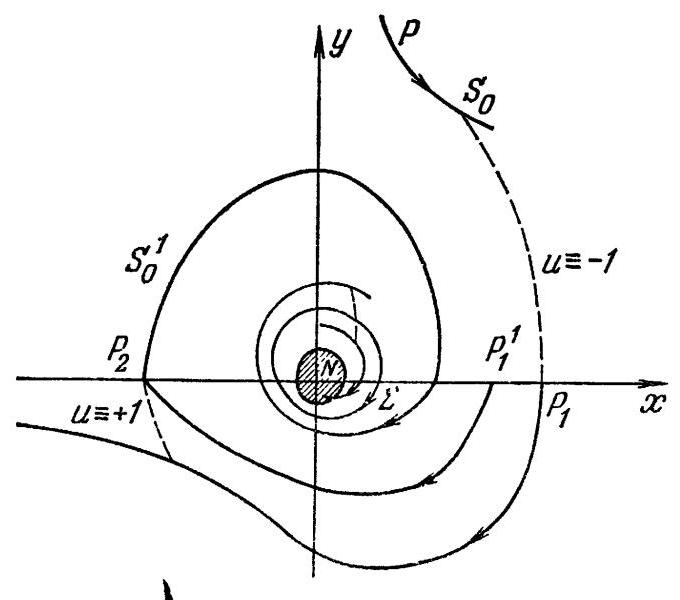
\includegraphics[max width=0.5\textwidth]{images/bo_d547k8bef24c73bgfcg0_466_207_480_680_600_0.jpg}
\end{center}
\hspace*{3em} 

Рис. 7.1. Построение области управляемости на плоскости при наличии восстанавливающей силы и неотрицательного трения.

Для того чтобы доказать существование оптимального управ- ления в Δ для каждой начальной точки \(P \in  {R}^{2}\) ,мы должны показать, пользуясь условием ограниченности из теоремы 4 главы 4, что решения системы S, которые начинаются в точке P и достигают начала координат до момента времени б, +1, где момент времени и задан заранее, не могут уйти далеко от начала координат.

\HRule

1) Поток векторного поля, определяемого системой „ \({\mathcal{S}}_{0}\) , через границу этой области был бы положительным, в то время как дивергенция этого поля, равная — ∂f/ду, всюду неположительна. (Прим. ред.)

\HRule

Пусть

\[
g\left( x\right)  = f\left( {x,0}\right) \text{ и }G\left( x\right)  = {\int }_{0}^{x}g\left( s\right) {ds} \geq  0.
\]

Monoxum

\[
E\left( {x,y}\right)  = \frac{{y}^{2}}{2} + G\left( x\right) .
\]

Toraa

\[
\dot{E} = y\left\lbrack  {g\left( x\right)  - f\left( {x,y}\right) }\right\rbrack   + u\left( t\right) y \leq  u\left( t\right) y.
\]

Поэтому

\[
\dot{E} \leq  \left| y\right|  \leq  \frac{{y}^{2}}{2} + 1 \leq  E + 1
\]

и

\[
E\left( t\right)  + 1 \leq  \left\lbrack  {E\left( {{x}_{0},{y}_{0}}\right)  + 1}\right\rbrack  {e}^{{t}_{1} + 1}
\]

вдоль любого решения, начинающегося в \(P = \left( {{x}_{0},{y}_{0}}\right)\) и определен- ного на некотором подынтервале времени из интервала 0≤ \(t \leq  {t}_{1} + 1\) . Итак

\[
\frac{{y}^{2}}{2} \leq  \left\lbrack  {E\left( {{x}_{0},{y}_{0}}\right)  + 1}\right\rbrack  {e}^{{t}_{1} + 1}
\]

и \(\left| {y\left( t\right) }\right|\) , a следовательно, и | \(x\left( t\right)\) | является ограниченным для всех таких решений системы Ф. Теорема доказана.

Для изучения систем дифференциальных уравнений с отталки- вающей силой мы предположим, что выполняются следующие условия (которые можно немного ослабить так же, как это сде- лано в теореме 3):

\[
\left( {\mathcal{G}}_{0}\right) \dot{x} = y,\;\dot{y} =  - f\left( {x,y}\right) ,\;f\left( {0,0}\right)  = 0,f\left( {x,y}\right)  \in  {C}^{1},
\]

где \(\frac{\partial f}{\partial x}\left( {x,0}\right)  <  - \varepsilon  < 0,\frac{\partial f}{\partial y} \geq  0\) для некоторого \(\varepsilon  > 0.\partial\) ra система имеет в начале координат единственную критическую точку. Вблизи начала координат семейство кривых—решений системы Г., — является топологически эквивалентным [Хартман] семейству кри- вых—решений линейной системы

(Y)
\[
\dot{x} = y,\;\dot{y} = x - y.
\]

Таким образом, имеются четыре кривые-решения системы \$0, кото- рые приближаются к началу координат при t → + ∞ или t → — ∞. Обозначим эти кривые символами I, II, III, IV соответственно квадрантам, в которых они лежат. Изучение геометрии системы G, показывает, что каждая из кривых I и III однозначно определена как функция на одной из полуосей х. Аналогично, кривые II и IV однозначно определены на некоторых подынтервалах оси х, причем \(\left| y\right|  \rightarrow  \infty\) с возрастанием |x|. Действительно, критическая точка и кривые \(I,{II},{III},{IV}\) ,и только они, являются сепаратрисами системы \$0, а остальная часть семейства кривых-решений систе- мы \$, состоит из четырех параллельных канонических областей [см. Маркус]. Поэтому система £, глобально гомеоморфна систе-

\[
\frac{\partial f}{\partial x}\left( {x,0}\right)  <  - \varepsilon  < 0,
\]

\[
\frac{\partial f}{\partial y}\left( {x,y}\right)  \geq  0\;\text{ в }\;{R}^{2}
\]

ме \(\mathcal{L}\) в \({R}^{2}\) . Cenaparpucis II и IV называются главными сепа- ратрисами системы \$0 (рис. 7.2).

\begin{center}
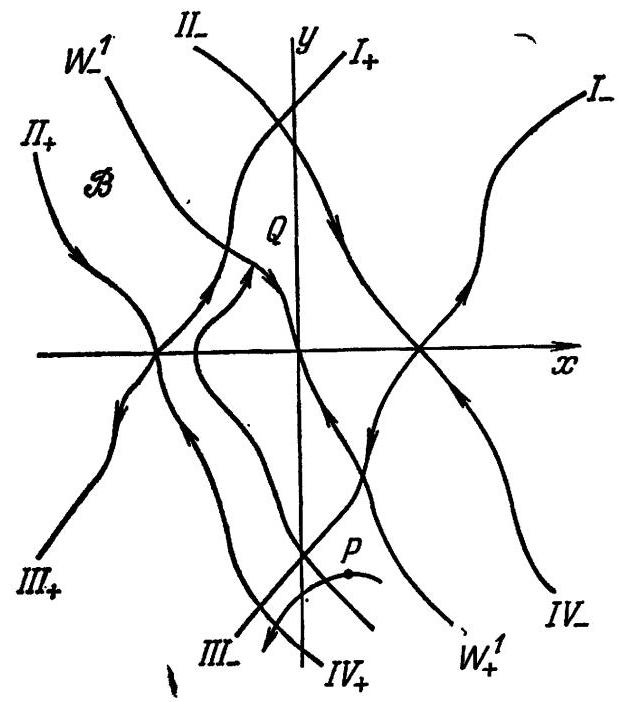
\includegraphics[max width=0.5\textwidth]{images/bo_d547k8bef24c73bgfcg0_468_206_392_620_702_0.jpg}
\end{center}
\hspace*{3em} 

Рис. 7.2. Область управляемости при на- личии отталкивающей силы и неотрица- тельного трения.

Теорема 4. Paccmompum систему

\[
\left( \mathcal{G}\right) \dot{x} = y,\dot{y} =  - f\left( {x,y}\right)  + u,
\]

\[
f\left( {0,0}\right)  = 0,f\left( {x,y}\right)  \in  {C}^{1},
\]

где и (t) — измеримая функция, удовлетворяющая ограничению \(- 1 \leq  u \leq  1,{\kappa a\kappa u}\) выше. Пред- положим, что f(x, y) ecmbo om- талкивающая сила с отрица- тельным трением, т. е.

Jog Hekomorozo E > 0, Toeda Kayk JAN 13 CUCMEM H H U H L zomeomophya numeuroù cucmeme \& u umeem cooumu cenapampucamu KDVBH | J | J | J | J | J | J | J | J | J | corresponding O6 acknow the Hyph-Indo-mononozureckou nonocou B, ozpakuuenkou Joyma nunuamu, zomeomop- фными прямым, одна из которых составлена из кривых II + и IV, состыкованных в критической точке системы \$+, а другая со- ставлена аналогично из кривых II- и IV\_. Кроме того, каждую точку из В можно перевести в начало координат оптимальным управлением и (t) ∈ Δ (см. рис. 7.2).

Доказательство. Каждая из систем

\[
\left( {\mathcal{Y} + }\right)
\]

\[
\dot{x} = y,\;\dot{y} =  - f\left( {x,y}\right)  + 1
\]

и

(f\_)
\[
\dot{x} = y,\;\dot{y} =  - f\left( {x,y}\right)  - 1
\]

имеет в точности одну критическую точку и четыре других сепа- ратрисы \({I}_{ \pm  },I{I}_{ \pm  },{II}{I}_{ \pm  },I{V}_{ \pm  }\) и является гомеоморфной системе Z. Далее, главные сепаратрисы \(I{I}_{ + },I{V}_{ + }\) и \(I{I}_{ - },{IV}{I}_{ - }\) вместе с двумя критическими точками систем \$+ и \$\_ ограничивают открытую полосу 8, которая гомеоморфна плоской полосе, расположенной между двумя параллельными линиями. Кроме того, область управ- ляемости ( совпадает с В.

Cenapaтрисы \({I}_{ + }\) и III\_ ограничивают относительно замкнутый криволинейный четырехугольник Q в 8 (см. рис. 7.2). Начальная точка из Q, которая переводится в начало координат при помощи управления \(u\left( t\right)  \in  \Delta\) ,не может покинуть \(Q\) во время своего пере- мещения в начало координат. Кроме того, начальная точка P из В, которая переводится в начало координат при помощи управления \(u\left( t\right)  \in  \Delta\) , никогда не может покинуть ограниченное множество, состоящее из объединения множества Q и подмно- жества 8 ограниченного: 1) решениями систем S+ и S\_, прохо- дящими через \(P\left( {t \geq  0}\right) ;2)\) граничными сепаратрисами полосы 8 и 3) краем множества Q, ближайшим к P. Таким образом, в лю- бом случае точка \(P\) и ее будущая траектория лежат в ограни- ченном подмножестве пространства R2. Такая априорная оценка гарантирует существование оптимального управления из \(\Delta\) для каждой начальной точки \(P\) в \(\mathcal{B} = \mathcal{C}\) . Теорема доказана.

\section*{Кривая переключений}

Рассмотрим задачу оптимального управления для системы

\[
\left( \mathcal{G}\right) x = y,\;\dot{y} =  - f\left( {x,y}\right)  + u,\;f\left( {0,0}\right)  = 0,f\left( {x,y}\right)  \in  {C}^{1},
\]

где \(u\left( t\right)\) — измеримая функция, удовлетворяющая ограничению \(- 1 \leq  u \leq  1\) ,как и выше. Если и (t) есть максимальное управле- ние из \(\Delta\) , то \(u\left( t\right)  = \operatorname{sgn}{\eta }_{2}\left( t\right)\) , где \(\eta \left( t\right)  = \left( {{\eta }_{1}\left( t\right) ,{\eta }_{2}\left( t\right) }\right)\) есть решение сопряженной системы

\[
{\dot{\eta }}_{1} = {\eta }_{2}\frac{\partial f}{\partial x},\;{\dot{\eta }}_{2} =  - {\eta }_{1} + {\eta }_{2}\frac{\partial f}{\partial y}.
\]

Определение. Рассмотрим множество максимальных релей- ных управлений в Δ для системы Я, переводящих точку области управляемости € в начало координат. Линия переключений W есть множество всех точек в €, в которых соответствующие ре- шения \(x\left( t\right)\) не имеют производных,т. е. \(W\) состоит из тех точек, в которых стыкуются \({\mathcal{G}}_{ + }\) - и \({\mathcal{G}}_{ - }\) -куски какой-либо максимальной траектории. Для определенности мы включаем начало коорди- нат в W.

Перейдем к описанию метода построения W. Пусть W+ есть решение (или дуга решения) системы \$, проходящего через начало координат и расположенного в четвертом квадранте х≥0, \(y \leq  0.\) Пусть \({W}^{1}\) есть решение (или дуга решения) системы \$\_, проходящего через начало координат и расположенного во втором квадранте \(x \leq  0,y \geq  0\) . Отложим теперь из каждой точки траек- тории \({W}_{ + }^{1}\) в направлении, обратном ходу времени, на соответ- ствующем решении системы 8- дугу, соответствующую промежутку времени, равному интервалу между нулями функции \({\eta }_{2}\left( t\right)\) . Это означает, что мы пользуемся решением системы уравнений

\[
{\dot{\eta }}_{1} = {\eta }_{2}\frac{\partial f}{\partial x}\left( {x\left( t\right) ,y\left( t\right) }\right) ,
\]

\[
{\dot{\eta }}_{2} =  - {\eta }_{1} + {\eta }_{2}\frac{\partial f}{\partial y}\left( {x\left( t\right) ,y\left( t\right) }\right) ,
\]

где \(x\left( t\right)  = \left( {x\left( t\right) ,y\left( t\right) }\right)\) —cootbertствующее решение системы \$\_, начинающееся на дуге \({W}_{ - }^{1}\) , a \({\eta }_{1}\left( 0\right)  =  - 1,{\eta }_{2}\left( 0\right)  = 0\) . [Отметим, что сопряженная линейная система является однородной и что мы начинаем траекторию х/с автономной системы \$\_ в момент времени \(t = 0\) .] Мы получаем первый нуль функции \({\eta }_{2}\left( t\right)\) в мо- мечт времени t/c), что определяет интервал времени, в течение, которого мы следуем вдоль решения х(t) системы g\_, начинаю- щегося на \({W}_{ + }^{1}\) . Геометрическое место в концов всех построенных таким образом дуг решений системы 8- с началом на дуге \({W}_{ + }^{1}\) мы обозначим через W2 и назовем отражением дуги W1.

Теперь из каждой точки дуги \({W}^{1}\) отложим в направлении, обратном ходу времени на соответствующем решении системы \({\mathcal{S}}_{ + }\) ,дугу, соответствующую промежутку времени, равному интер- валу между нулями функции \({\eta }_{2}\left( t\right)\) . Это означает, что мы пользу. емся решением системы уравнений

\[
{\dot{\eta }}_{1} = {\eta }_{2}\frac{\partial f}{\partial x}\left( {x\left( t\right) ,y\left( t\right) }\right) ,
\]

\[
{\dot{\eta }}_{2} =  - {\eta }_{1} + {\eta }_{2}\frac{\partial f}{\partial y}\left( {x\left( t\right) ,y\left( t\right) }\right) ,
\]

где \(x\left( t\right)  = \left( {x\left( t\right) ,y\left( t\right) }\right)\) -соответствующее решение: системы \({\mathcal{S}}_{ + }\) , начинающееся на дуге \({W}^{1}\) , a \({\eta }_{1}\left( 0\right)  = 1,{\eta }_{2}\left( 0\right)  = 0\) . Как и выше, мы встречаем первый нуль функции \({\eta }_{2}\left( t\right)\) в момент времени t/c. Обозначим отражение множества W1 с помощью системы \$+. через \({W}_{ + }^{2}\) .

Пусть теперь \({W}_{ + }^{1},{W}_{ + }^{2},\ldots ,{W}_{ + }^{k}\) и \({W}_{ - }^{1},{W}_{ - }^{2},\ldots ,{W}_{ - }^{k}\) опре- делены, и пусть W+1 есть отражение траектории W* с помощью системы \({\mathcal{S}}_{ + }\) , a \({W}^{k + 1}\) -отражение траектории \({W}_{ + }^{k}\) с помощью си- стемы \$\_, построенное как указано выше. Конечно, может слу- читься, что множество \({W}_{ + }^{k} \cup  {W}_{ - }^{k}\) окажется пустым для любого достаточно большого \(k\) .

Teopeмa 5. Рассмотрим систему(\$)

\[
\left( \mathcal{C}\right) x = y,\;y =  - f\left( {x,y}\right)  + u,\;f\left( {0,0}\right)  = 0,f\left( {x,y}\right)  \in  {C}^{1}
\]

с измеримыми управлениями и (t), удовлетворяющими ограничению \(- 1 \leq  u \leq  1\) . Линия переключений W есть в точности объединение множеств W+UW по h=1,2,3,…

Доказательство. Пользуясь теоремой 1, получаем, что для каждой точки \(P\) траектории \({W}_{ + }^{1}\left( {y < 0}\right)\) мы можем выбрать сопряженное решение η (t) = ( \({\eta }_{1}\left( t\right) ,{\eta }_{2}\left( t\right)\) ) так, чтобы функция \({\eta }_{0}\left( t\right)\) обращалась в нуль, когда х(t) =P и нигде более. Анало- гично, если Р есть концевая точка W+1, а у =0, мы можем вы- брать \(\eta \left( t\right)\) так, что функция \({\eta }_{2}\left( t\right)\) обращается в нуль в моменты времени, соответствующие \(x\left( t\right)  = P\) и \(x\left( t\right)  = 0\) . Тогда каждая точ- ка из \({W}_{ + }^{1}\) ,включая концевые, может оказаться точкой переклю- чения для решения, соответствующего максимальному релейному управлению в Δ. Таким образом, \({W}_{ + }^{1} \subset  W\) и аналогично \({W}_{ - }^{1} \subset  W\) .

Так как каждому максимальному релейному управлению, которое переводит точку из \(\mathfrak{C}\) в начало координат, должно соответствовать решение, которое входит в начало координат вдоль одной из кри- вых W+ или W-1, и так как решение должно состоять из чере- дующихся кусков кривых, представляемых семейством решений \({\mathcal{S}}_{ + }\) или \({\mathcal{S}}_{ - }\) , с переключениями, происходящими в нулях функции \({\eta }_{2}\left( t\right)\) , to мы видим,что \(W\) есть объединение всех \({W}_{ + }^{k}\) и \({W}_{ - }^{k}\) для \(k = 1,2,3,\ldots\) Теорема доказана.

\section*{Синтез оптимального управления для случая притягивающей силы}

Мы рассмотрим здесь синтез оптимального управления для системы с одной степенью свободы, к которой приложена при- тягивающая сила. Итак, рассмотрим систему(\$)

\[
\left( \mathcal{G}\right) \dot{x} = y,\dot{y} =  - f\left( {x,y}\right)  + u,\;f\left( {0,0}\right)  = 0,\;f\left( {x,y}\right)  \in  {C}^{1},
\]

где управление и (t) является измеримой функцией с ограничением \(- 1 \leq  u \leq  1,\) u

\[
\frac{\partial f}{\partial x}\left( {x,0}\right)  > \varepsilon  > 0,\;\frac{\partial f}{\partial y}\left( {x,y}\right)  \geq  0
\]

для некоторого ε>0. Эти предположения, до некоторой степени более сильные, чем предположения теоремы 3, гарантируют, что каждая из максимальных систем \$+ и \$\_ имеет в точности одну критическую точку, и вообще упрощают изложение задачи. Так, например, каждое решение системы G±, кроме единственной кри- тической точки, есть или периодическое решение, или же накру- чивается как спираль на предельный цикл, или, наконец, стремится к критической точке при t→+∞. Если к тому же ∂f/ду > 0, то из условия Бендиксона следует, что здесь не имеется предель- ных циклов.

Теорема 6. Рассмотрим систему

(\$)
\[
x = y
\]

\[
y =  - f\left( {x,y}\right)  + u,f\left( {0,0}\right)  = 0,f\left( {x,y}\right)  \in  {C}^{2},
\]

\(e\partial e\frac{\partial f}{\partial x}\left( {x,0}\right)  > \varepsilon  > 0\;\partial n.A\;\) некоторого \(\varepsilon  > 0,\frac{\partial f}{\partial y} \geq  0\;\text{ в }\;{R}^{2}\) . Pac- смотрим, далее, максимальные управления и (i) Е 𝑑, переводящие точки из 8 – 8 в начало координат, и построим линию переклю- чения W как объединение множеств W + W *, как описано в тео- реме 5. Тогда множество W содержит гомеоморфный образ прямой, который является кусочно-гладкой кривой, разделяющей плоскость. Кроме того, множество W лежит целиком во втором и четвертом квадрантах.

Доказательство. Линия переключения W совпадает с объеди- нением \({W}_{ + }^{k} \cup  {W}_{ - }^{k}\) по \(k = 1,2,3\ldots\) Конечно, \({W}_{ + }^{1}\) и \({W}_{ - }^{1}\) —кривые класса \({C}^{2}\) . Так как сопряженный интервал времени, использован- ный в процессе отражения, гладко зависит от начальных условий, то ясно, что W+ и W- являются кривыми класса С1. Аналогично, \({W}_{ + }^{k}\) и \({W}_{ - }^{k}\left( {k = 1,2,3,\ldots }\right)\) являются кривыми класса \({C}^{1}\) ,и гладко зависят от начальных условий.

Мы покажем теперь, что множество W содержит гомеоморфный образ прямой, который разделяет плоскость. Для простоты изложе- ния сначала рассмотрим консервативный случай, когда дf/ду≡ 0 в \({R}^{2}\) . В этом случае каждое решение системы \$+, кроме критической точки, есть периодическое решение, охватывающее критическую точку. Легко также видеть, что каждое такое периодическое ре- шение есть выпуклая замкнутая кривая, симметричная относительно оси х. При \(y > 0\) имеем

\[
\frac{\dot{y}}{\dot{x}} = {y}^{\prime } = \frac{dy}{dx} = \frac{-f\left( x\right)  + u}{y}
\]

H

\[
\frac{{d}^{2}y}{d{x}^{2}} = \frac{-y{f}^{\prime }\left( x\right)  - {\left\lbrack  f\left( x\right)  - u\right\rbrack  }^{2}/y}{{y}^{2}} < 0.
\]

Аналогично, при \(y < 0\) мы получим, что \({y}^{\prime \prime } > 0\) , orжуда легко следует, что периодическое решение выпукло и симметрично в смысле, указанном выше.

Пусть \({S}_{ + }^{1}\) есть решение системы \({\mathcal{S}}_{ + }\) ,проходящее через начало координат так, что \({W}_{ + }^{1}\) есть дуга кривой \({S}_{ + }^{1}\) . Обозначим через \({R}_{1}\) правую точку пересечения дуги \({W}_{ + }^{1}\) с осью х. Пусть аналогично \({S}_{ - }^{1}\) есть решение системы f\_, проходящее через начало координат, \({W}^{1}\) —ero дуга (см. рис. 7.3), а \({L}_{1}\) —левая точка пересечения дуги \({W}^{1}\) c ocbo \(x\) . Пусть \({S}_{ - }^{2}\) —решение системы f\_, проходящее через точку \({R}_{1}\) , a \({S}_{ + }^{2}\) —решение системы \({\mathcal{S}}_{ + }\) ,проходящее через точку \({L}_{1}\) .

Пусть \({S}_{ + }^{k}\) и \({S}_{ - }^{k},k = 1,2,\ldots\) , определенные аналогично тому как указано выше, решения систем \$+ и \$\_, соответственно, а \({R}_{k}\) и \({L}_{k}\) —аналогично определенные точки оси х, так что \({\mathcal{S}}^{k + 1}\) есть решение системы \$\_, проходящее через точку R, a S+1 есть решение системы \({\mathcal{S}}_{ + }\) , проходящее через точку \({L}_{k}\) . Легко видеть, что решение S+ лежит внутри области, ограниченной решением \({S}_{ + }^{k + 1}\) . Аналогичное замечание можно сделать по поводу взаимного расположения решений \({S}_{ - }^{k}\) и \({S}_{ - }^{k + 1}\) . Далее,

\[
0 < {R}_{1} < {R}_{2} < \ldots  < {R}_{k} \rightarrow   + \infty
\]

H

\[
0 > {L}_{1} > {L}_{2} > \ldots  > {L}_{k} \rightarrow   - \infty \text{ . }
\]

Теперь мы опишем множество W для каждого сегмента [0, R], \(\left\lbrack  {{R}_{1},{R}_{2}}\right\rbrack  ,\ldots \left\lbrack  {{R}_{k},{R}_{k + 1}}\right\rbrack  \ldots ,\mathrm{c}\) тем,чтобы получить непрерывную кривую, определенную при \(x \geq  0\) и лежащую в четвертом квадранте. Затем аналогично построим кривую W для \(x \leq  0\) .

\begin{center}
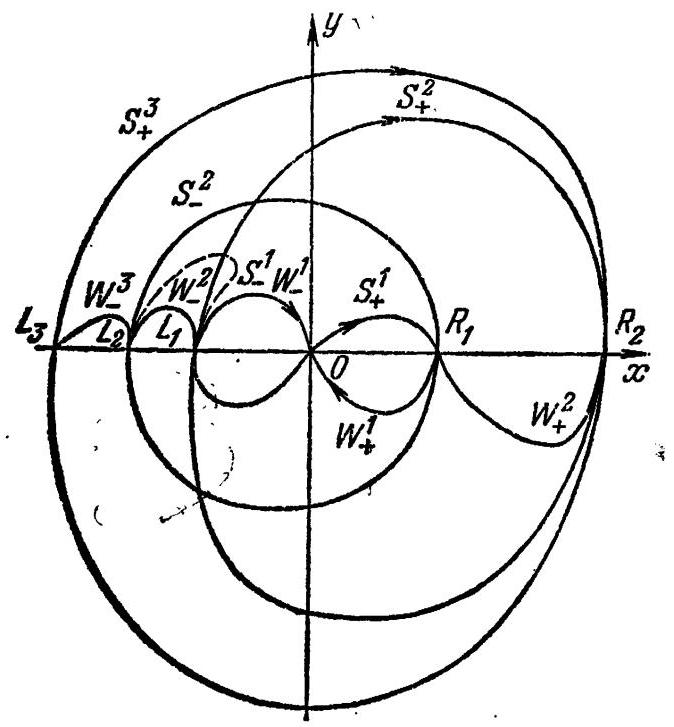
\includegraphics[max width=0.6\textwidth]{images/bo_d547k8bef24c73bgfcg0_473_750_488_674_727_0.jpg}
\end{center}
\hspace*{3em} 

Рис. 7.3. Кривая переключения для случая нелинейной восстанавливающей силы.

Положим на отрезке \(\left\lbrack  {0,{R}_{1}}\right\rbrack  W = {W}_{ + }^{1}\) . По теореме 1, дуга \({W}_{ + }^{2}\) , coed积няющая точ- ки \({R}_{1}\) и \({R}_{2}\) и лежащая между траекториями \({S}_{ + }^{1}\) и \({S}_{ + }^{2}\left( {y \leq  0}\right)\) , есть кривая класса \({C}^{1}\) . Ана- логично, дуга \({W}^{2}\) , соединяю- щая точки \({L}_{1}\) c \({L}_{2}\) и лежащая между траекториями \({S}_{ - }^{1}\) и \({S}_{ - }^{2}\) при \(y \geq  0\) , есть кривая клас- ca \({C}^{1}\) . \(\Pi\) ou индукции мы нахо- дим, что \({W}^{k}\) есть кривая клас. ca \({C}^{1}\) , coedиняющая точки \({L}_{k - 1}\) c \({L}_{k}\) и лежащая между траекториями \({S}_{ - }^{k - 1}\) и \({S}_{ - }^{k}\) в обла- сти у е о, а W + есть кривая класса \({C}^{1}\) , coeдиняющая точки \({R}_{k - 1}\) c \({R}_{k}\) и лежащая между реше- ниями \({S}_{ + }^{k - 1}\) и \({S}_{ + }^{k}\) в области \(y \leq  0\) для любого \(k = 2,3,4,\ldots\) Taким образом, \(W = {\bigcup }_{k = 1}^{\infty }\left( {{W}_{ + }^{k} \cup  {W}_{ - }^{k}}\right)\) есть счетное объединение кри- вых класса \({C}^{1}\) и W разделяет плоскость на две части.

Случай, когда ∂f/ду ≢ 0, рассматривается аналогично, за исклю- чением того, что здесь \({S}_{ + }^{1}\) или \({\widetilde{S}}_{ - }^{1}\) или одно из последующих отражений \({W}_{ \pm  }^{k}\) может иметь концевую точку в ±∞,т. е. шк мо- жет не пересекать оси х, а стремиться к бесконечности. В таком случае совокупность непустых множеств может быть конечной (см. рис. 7.4). Однако утверждения теоремы справедливы и для этого случая. Теорема доказана.

\section*{Специальные гипотезы относительно геометрии линии переключения}

Мы здесь вынуждены предположить, что линия переключения \(W = W\left( x\right)\) определяется однозначной функцией, определенной на оси х. Это, конечно, справедливо, если кривые \({W}_{ + }^{1}\) и \({W}_{ - }^{1}\) уходят в бесконечность, не пересекаясь с осью х, как в случае системы с отталкивающей силой (см. теорему 4). В качестве иллюстрации рассмотрнм систему

\[
\ddot{x} + b\dot{x} + {g}_{1}\left( x\right)  = u\left( t\right) ,\; - 1 \leq  u\left( t\right)  \leq  1,
\]

где \(b > 0\) — постоянная величина и я у (х) кек у один я у оде \({g}^{\prime }\left( x\right)  > 0,\left| {g\left( x\right) }\right|  > 1\) для всех х с достаточно большим \(\left| x\right|\) . Далее

Если бы кривая \({W}_{ + }^{1}\) пересекала ось х более, чем в одной точке, то уравнение в вариациях, по- строенное для \(x\left( t\right)  = {W}_{ + }^{1}\) ,имело мы предположим, что gives \({b}^{2}\left( x\right)  \leq  {b}^{2}/4\) при (— \(\infty  < x <  + \infty\) ). В качестве примера системы с такой слабой упругой силой и линейным тре- HHEM BO3bMEM CHCTEMY

\[
\ddot{x} + 2\dot{x} + \left( {x - \frac{1}{2}\operatorname{Arctg}x}\right)  = u\left( t\right) ,
\]

\[
- 1 \leq  u\left( t\right)  \leq  1,
\]

\begin{center}
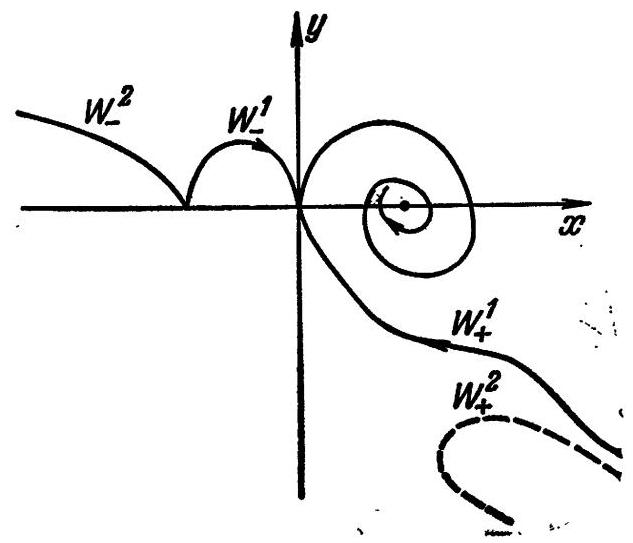
\includegraphics[max width=0.5\textwidth]{images/bo_d547k8bef24c73bgfcg0_474_214_478_633_543_0.jpg}
\end{center}
\hspace*{3em} 

Рис. 7.4. Кривая переключения с дугами, уходящими в бесконечность.

где

\[
- \frac{\pi }{2} < \operatorname{Arctg}x < \frac{\pi }{2}.
\]

бы решение в варианиях уравнение в вариациях

\[
\ddot{v} + b\dot{v} + {g}^{\prime }\left( {x\left( t\right) }\right) v = 0
\]

при помощи подстановки \(z = {e}^{{bt}/2}v\) приводится к виду

\[
\ddot{z} + \left( {{g}^{\prime }\left( {x\left( t\right) }\right)  - \frac{{b}^{2}}{4}}\right) z = 0.
\]

Но нетривиальное решение z (t) этого уравнения имеет не более одного нуля. Отсюда следует, что кривая \({W}_{ + }^{1}\) не пересекает поло- жительную полуось х, и простая оценка ее наклона показывает, что кривая \({W}_{ + }^{1}\) определена для всех х > 0. Аналогично, кривая W1 является однозначной на отрицательной полуоси х.

Максимальное решение вне множества W (х) =W U+ W + имеет никаких переключений. Это следует из вида присоединен- ного уравнения

\[
{\ddot{\eta }}_{2} - b{\dot{\eta }}_{2} + {g}^{\prime }\left( {x\left( t\right) }\right) {\eta }_{2} = 0.
\]

Поэтому линия переключений есть в точности

\[
W\left( x\right)  = {W}_{ - }^{1} \cup  {W}_{ + }^{1}
\]

и сделанные выше особые предположения в этом случае выпол- няются. Они выполняются также, когда система \$4 имеет лишь изохронные периодические решения, например, в случае, когда \(f\left( {x,y}\right)  = x\) . В этом случае уравнение в вариациях вдоль решений системы S+ или S\_ имеет вид

\[
{\dot{v}}^{1} = {v}^{2},\;{\dot{v}}^{2} =  - \frac{\partial f}{\partial x}{v}^{1} - \frac{\partial f}{\partial y}{v}^{2},
\]

где v (t) = (v (t), v²(t)) —вектор параллельного смещения вдоль потока систем \({\mathcal{G}}_{ \pm  }\) . Но

\[
{v}^{1}{\eta }_{1} + {v}^{2}{\eta }_{2} = \text{ const }
\]

II, ТАКHM O6pa3OM,

\[
{v}^{1}\left( 0\right) {\eta }_{1}\left( 0\right)  = {v}^{1}\left( {t}_{1}\right) {\eta }_{1}\left( {t}_{1}\right)
\]

для двух последовательных моментов переключения \(t = 0\) и \(t = {t}_{1}\) . Так как

\[
{\eta }_{1}\left( 0\right) {\eta }_{1}\left( {t}_{1}\right)  < 0,
\]

ТО

\[
{v}^{1}\left( 0\right) {v}^{1}\left( {t}_{1}\right)  \leq  0
\]

Поэтому, взяв в качестве v (0) касательный вектор к траектории \({W}_{ \pm  }^{k}\) ,получим,что \(v\left( {t}_{1}\right)\) есть также касательный вектор к траек- тории \({W}_{ \pm  }^{k + 1}\) и, поэтому кривая \({W}_{ \pm  }^{k + 1}\) определяется однозначной на оси х функцией, если кривая \({W}_{ \pm  }^{k}\) обладает этим свойством. Tenepb (по индукции) можно показать, что W = W (х) является однозначной функцией на оси х.

Cледствие. Рассмотрим систему S/ теоремы 6. Предполо- жим, что кривая \(W = W\left( x\right)\) onpedвляется однозначной функцией на оси х. Тогда для каждой точки РЕ Рг в а имеется одно и только одно максимальное релейное управление, которое переводит точку Р в начало координат.

Доказательство. Мы должны только показать, что ника- кая траектория \(S\) системы G- (или \({\mathcal{G}}_{ + }\) ) не пересекается с кривой \({W}_{ + }^{k}\) (или с кривой \({W}_{ - }^{k}\) ) по внутренней точке дуги (траектории S), использованной при построении кривой \({W}_{ + }^{k}\) (или \({\widehat{W}}_{ - }^{k}\) ). Так как кривая \({W}_{ + }^{k}\) лежит в области \(y < 0\) целиком, за исключением своих концевых точек, то решение 8 системы f\_, начинающееся в точке P кривой \({W}_{ + }^{k}\) ,не может пересечь кривую \({W}_{ + }^{k}\) в области у <0 в ка- кой-нибудь точке, абсцисса х которой лежит левее P. Кроме того, так как в соответствующей кольцевой области на каждом решении системы У. имеется только одна точка кривой \({W}_{ + }^{k}\) и, так как решения системы \$\_ имеют отрицательный касательный вектор \(\left( {-y,f + 1}\right)\) в противоположность вектору (− \(y,f - 1\) ) для реше. ний системы у., то получаем, что траектория \(\mathcal{S}\) не может пере. сечь кривой \({W}_{ + }^{k}\) в полуплоскости \(y < 0\) .

Аналогичное рассуждение справедливо для решений системы G+ пересекающих кривую W-. Следствие доказано.

Теорема 7. Paccмотрим систему

\(\left( \mathcal{S}\right) \dot{x} = y,\;\dot{y} =  - f\left( {x,y}\right)  + u,\;f\left( {0,0}\right)  = 0,\;f\left( {x,y}\right)  \in  {C}^{1}, \; e\partial e\frac{\partial f}{\partial x}\left( {x,0}\right)  > \varepsilon  > 0\;\partial n\;{ne\kappa omopo\text{ г }o}\;\varepsilon  > 0\;u\;\frac{\partial f}{\partial y} \geq  0\;e\;{R}^{2}\) . Предположим, что функция \(W = W\left( x\right)\) однозначна на оси х. Тогда для каждой точки \(P\) в \({R}^{2}\) имеется в точности одно оптимальное управление \(u\left( t\right) \left( {-1 \leq  u \leq  1}\right)\) из \(\kappa\) ласса ∆, \(\kappa\) omo poe переводит точку Р в начало координат. Определим синтезирующую функцию

\[
\Psi \left( {x,y}\right)  = \left\{  \begin{aligned} 1 & \partial \Omega \mathfrak{A}x & y < W\left( x\right) , \\  0 & \partial \Omega \mathfrak{A}y &  = W\left( x\right) , \\   - 1 & \partial \Omega \mathfrak{A}y &  > W\left( x\right) . \end{aligned}\right.
\]

Тогда искомая оптимальная траектория для точки P есть един- ственное решение уравнения

\[
\ddot{x} + f\left( {x,\dot{x}}\right)  = \Psi \left( {x,\dot{x}}\right) ,
\]

соответствующее начальному условию x (0) = P.

Доказательство. Согласно общей теории существования оптимального и, тем самым, максимального релейного управления, развитой выше, каждая точка \(P \in  {R}^{2}\) лежит по крайней мере на одной траектории, соответствующей максимальному релейному управлению, переводящему точку P в начало координат. Но кон- струкция, использованная в теореме 6 вместе со следствием, пока- зывает, что точка \(P\) лежит на единственной траектории, соответ- ствующей такому максимальному релейному управлению и, следо- вательно, это управление должно быть единственным оптимальным управлением из класса Δ для точки P.

Из теоремы 6 следует, что синтезирующая функция \(\Psi \left( {x,y}\right)\) обладает нужными свойствами. Теорема доказана.

\section*{Синтез оптимального управления для случая отталкивающей силы}

Рассмотрим задачу управления для системы

\[
\text{ (S) }\dot{x} = y,\dot{y} =  - f\left( {x,y}\right)  + u,f\left( {0,0}\right)  = 0,f\left( {x,y}\right)  \in  {C}^{1}\text{ , }
\]

где \(u\left( t\right)\) — измеримая функция ( — 1 ≤ u ≤ l ). Предположим, что \(\frac{\partial f}{\partial x}\left( {x,y}\right)  <  - \varepsilon  < 0,\frac{\partial f}{\partial y}\left( {x,y}\right)  \geq  0\) для некоторого \(\varepsilon  > 0\) . Эти пред- положения, до некоторой степени более сильные, чем предполо- жения теоремы 4, гарантируют существование полосы 8 между главными сепаратрисами систем Я, и Я, и, которая является областью \(\mathfrak{C}\) нуль-управляемости системы Я. Для каждой точки \(P \in  \mathcal{B}\) существует оптимальное управление и (t) из допустимого класса \(\Delta\) ,которое переводит Р в начало координат.

Линия переключений W системы \$ определяется так же, как и в теореме Б. Перейдем к построению W. Пусть W+ решение системы <\_<u походящее через начало координат и лежащее в четвертом квадранте. Путем сравнения наклонов траекторий систем \({\mathcal{S}}_{ + }\) и \({\mathcal{S}}_{ - }\) мы обнаружим,что \({W}_{ + }^{1}\) лежит всегда внутри полосы 8, в полуплоскости у <0, и что у \(\rightarrow   - \infty\) с ростом \(x\) вдоль кривой \({W}_{ + }^{1}\) . Пусть \({W}_{ - }^{1}\) -решение системы f\_, проходящее через начало координат и лежащее во втором квадранте. Ясно, что кривая \({W}^{1}\) -лежит внутри 8 и что у — хо с ростом (—х), если \(\left( {x,y}\right)  \in  {W}^{1}\) . Orpawekния \({W}_{ \pm  }^{k}\) onpedgeляются как в теореме 5, но мы покажем, что все эти отражения являются пустыми мно- жествами для \(k = 2,3,4,\ldots ,u\) что,тем самым, \(W = {W}_{ + }^{\prime } \cup  {W}_{ - }^{1}\) (см. рис. 7.2).

Теорема 8. Рассмотрим систему

\(\left( \mathcal{S}\right) \dot{x} = y,\;\dot{y} =  - f\left( {x,y}\right)  + u,\;f\left( {0,0}\right)  = 0,\;f\left( {x,y}\right)  \in  {C}^{1},\)

\(e\partial e\frac{\partial f}{\partial x}\left( {x,y}\right)  <  - \varepsilon  < 0,\frac{\partial f}{\partial y}\left( {x,y}\right)  \geq  {0\varepsilon }{R}^{2}\partial n \neq  {ne\kappa }\) omoрozo \(\varepsilon  > 0.\) Рассмотрим максимальное релейное управление и (t) (— 1 ≤ u ≤ 1) из класса ∆, и построим линию переключения W. Тогда W = W (x) есть непрерывная однозначная функция на сегменте оси х, раз- бивающая область В на две подобласти. Кроме того,

\[
W\left( x\right)  = \left\{  \begin{array}{ll} {W}_{ + }^{1}\left( x\right) & \partial \Omega \mathfrak{A}x \geq  0, \\  {W}_{ - }^{1}\left( x\right) & \partial \Omega \mathfrak{A}x \leq  0, \end{array}\right.
\]

\(\max\) что W (x) \(\in  {C}^{1}\) при \(x \neq  0\) .

Доказательство. Мы сначала докажем, что множества W± являются пустыми. Это будет в том случае, если нетривиальное perueние \(\eta \left( t\right)  = \left( {{\eta }_{1}\left( t\right) ,{\eta }_{2}\left( t\right) }\right)\) cucтемы

\[
{\dot{\eta }}_{1} = {\eta }_{2}\frac{\partial f}{\partial x}\left( {x\left( t\right) ,y\left( t\right) }\right) ,
\]

\[
{\dot{\eta }}_{2} =  - {\eta }_{1} + {\eta }_{2}\frac{\partial f}{\partial y}\left( {x\left( t\right) ,y\left( t\right) }\right)
\]

таково, что функция \({\eta }_{2}\left( t\right)\) имеет не более одного нуля. Здесь \(\mathbf{x}\left( t\right)  = \left( {x\left( t\right) ,y\left( t\right) }\right)\) есть решение системы \$\_ или \$\_+. Пусть \({t}_{1},{t}_{2}\left( {{t}_{1} < {t}_{2}}\right)\) два последовательных нуля функции \({\eta }_{2}\left( t\right)\) и пусть \({\eta }_{2}\left( t\right)  > 0\) при \({t}_{1} < t < {t}_{2}\) . Тогда \({\eta }_{1}\left( {t}_{1}\right)  < 0\) и \({\eta }_{1}\left( {t}_{2}\right)  > 0\) . Так \(\kappa\) ак \(\partial f/\partial x <  - \varepsilon  < 0\) , то \({\dot{\eta }}_{1}\left( t\right)  < 0\) при \({t}_{1} < t < {t}_{2}\) , что невозможно. Аналогично рассматривается случай \({\eta }_{2}\left( t\right)  < 0\left( {{t}_{1} < t < {t}_{2}}\right)\) . По- скольку в силу теоремы \(5{W}_{ + }^{1} \cup  {W}_{ - }^{1} \subset  \bar{W}\) ,то

\[
W = W\left( x\right)  = \left\{  \begin{array}{lll} {W}_{ + }^{1}\left( x\right) & \text{ для } & x \geq  0, \\  {W}_{ - }^{1}\left( x\right) & \text{ для } & x \leq  0. \end{array}\right.
\]

Ясно, что W есть топологический образ прямой, и что W разби- вает полосу 8 на две части. Теорема доказана.

Cледстви e. Рассмотрим систему \$ теоремы 8. Тогда для каждой точки \(P \in  \mathcal{B}\) имеется одно и только одно максимальное релейное управление в ∆, которое переводит точку Р в начало координат.

Доказательство. Никакое решение системы Я\_ не может пересечь \({W}_{ + }^{1}\) в двух различных точках, как это следует из срав- нения наклонов касательных векторов решений систем \({\mathcal{L}}_{ + }\) и \({\mathcal{L}}_{ - }\) . Аналогичное утверждение справедливо и относительно кривой W1. Конструкция линии W показывает, что каждому максимальному релейному управлению из класса ∆, переводящему P ∈ ® в начало координат, соответствует траектория, которая пересекает кривую W и затем никогда не покидает \(W\) , a следует по \(W\) в начало коор- динат. Следствие доказано.

Теорема 9. Paccmompum cucmeuf

\(\left( \mathcal{S}\right) \dot{x} = y,\;\dot{y} =  - f\left( {x,y}\right)  + u,\;f\left( {0,0}\right)  = 0,\;f\left( {x,y}\right)  \in  {C}^{1},\)

\(e\partial e\frac{\partial f}{\partial x}\left( {x,y}\right)  <  - \varepsilon  < 0\partial n.\pi\) не которого \(\varepsilon  > 0\;u\frac{\partial f}{\partial y}\left( {x,y}\right)  \geq  0\;\varepsilon {R}^{2}.\) Рассмотрим далее область € = В управляемости для измеримых управлений \(u\left( t\right) \;\left( {-1 \leq  u \leq  1}\right) \;{u3}\;\Delta \;u\) nocmpoum линию пере- ключения \(W = W\left( x\right)\) .

Тогда для каждой точки РЕ В существует только одно опти- мальное управление и (t) из класса ∆, которое переводит точку Р в начало координат. Определим синтезирующую функцию

\[
\Psi \left( {x,y}\right)  = \begin{cases} 1 & \partial n\mathfrak{A}y < W\left( x\right) , \\  0 & \partial n\mathfrak{A}y = W\left( x\right) , \\   - 1 & \partial n\mathfrak{A}y > W\left( x\right) . \end{cases}
\]

Тогда оптимальная траектория для P есть (единственное) реше- ние уравнения

\[
\ddot{x} + f\left( {x,\dot{x}}\right)  = \Psi \left( {x,\dot{x}}\right)
\]

с начальным условием x (0) = P.

Доказательство. Общая теория оптимального и макси- мального управления, развитая выше, показывает, что каждая точка \(P \in  \mathcal{B}\) лежит по крайней мере на одной траектории макси- мального управления, переводящей P в начало координат. Но построения теоремы 8, вместе со следствием, показывают, что точка \(P\) лежит на единственной траектории такого максимального релейного управления и, следовательно, это управление должно быть единственным оптимальным управлением класса ∆ для P.

Из построений теоремы 8 следует, что функция \(\Psi \left( {x,y}\right)\) обла- дает нужными свойствами. Теорема доказана. Примеры построения управлений с обратной связью

Пример 1 (жесткая пружина). Рассмотрим уравнение Дуф- финга с управлением

\[
\ddot{x} + x + 2{x}^{3} = u\left( t\right)
\]

или эквивалентную систему первого порядка:

\[
\left( {\mathcal{L}}_{d}\right)
\]

\[
\dot{x} = y,\;\dot{y} =  - x - 2{x}^{3} + u,
\]

где — \(1 \leq  u \leq  1\) . Эта система есть математическая модель, описы- вающая поведение нелинейной жесткой пружины под действием внешней силы и (t).

Для задачи оптимального быстродействия оптимальное управ- ление \(u\left( t\right)\) на различных интервалах времени равно +1 или -1. Поэтому рассмотрим систему уравнений

\[
\left( {\mathcal{Y} \pm  }\right)
\]

\[
\dot{x} = y,\;\dot{y} =  - x - 2{x}^{3} \pm  1.
\]

Ясно, что каждая точка в фазовом пространстве может быть со- единена с началом координат кривой, состоящей из кусков траек- торий систем \({\mathcal{S}}_{ + }\) и \({\mathcal{S}}_{ - }\) ,что гарантирует нам существование опти- мального управления. Рассмотрим теперь сопряженную систему (как и в предыдущем случае)

(A)
\[
{\dot{\eta }}_{1} =  - \frac{\partial H}{\partial x} = {\eta }_{2}\left( {1 + 6{x}^{2}\left( t\right) }\right) ,\;{\dot{\eta }}_{2} =  - \frac{\partial H}{\partial y} =  - {\eta }_{1},
\]

из которой мы найдем функцию \({\eta }_{2}\left( t\right)\) , ompeделяющую интервалы времени, на которых максимальная траектория совпадает с траек- ториями того или другого семейства.

Построим теперь линию переключения W способом, указанным в предшествующей теории. Здесь \({W}_{ + }^{1}\) есть решение системы \({\mathcal{S}}_{ + }\) , проходящее через начало координат и лежащее в четвертом квад- ранте (см. рис. 7.5), a Wi есть решение системы f\_, проходящее через начало координат и лежащее во втором квадранте.

Мы теперь построим отражение кривой \({W}^{1}\) с помощью системы \({\mathcal{L}}_{ + }\) . Из точек 1, 2, ..., 9 кривой W1 следуем вдоль соответст- вующих решений системы \$+ в направлении обратному ходу вре- мени в течение промежутков времени, равных интервалу между нулями функции \({\eta }_{2}\left( t\right)\) ,т. e. например, из точки 2 (η,(0)=1, \({\eta }_{2}\left( 0\right)  = 0)\) следуем вдоль соответствующего решения \({\mathcal{S}}_{ + }\) до тех пор, пока у 2 не будет, снова нулем. Это определяет точку 2а на кривой \({W}_{ + }^{2}\) . Повторив эту процедуру для каждой из точек \(3,\ldots ,9\) ,мы получим соответствующие точки \({3a},\ldots ,{9a}\) кри- вой \({W}_{ + }^{2}\) . Так как мы знаем,что \({W}_{ + }^{2}\) есть кривая класса \({C}^{1}\) , ТО мы можем проинтерполировать ее гладкой кривой, соединяющей \({2a},{3a},\ldots ,{8a}\) . По этой причине требуется рассмотрение лишь конечного числа максимальных траекторий для построения линии W.

Теперь, когда кривая \({W}_{ + }^{2}\) построена, мы можем получить кри- вую W2 отражением кривой W2 относительно начала координат (рис. 7.5). Далее мы находим W3 переносом кривой W4 вдоль решений системы S+, как указано выше. Остальные дуги кривой W строятся точно таким же образом.

\begin{center}
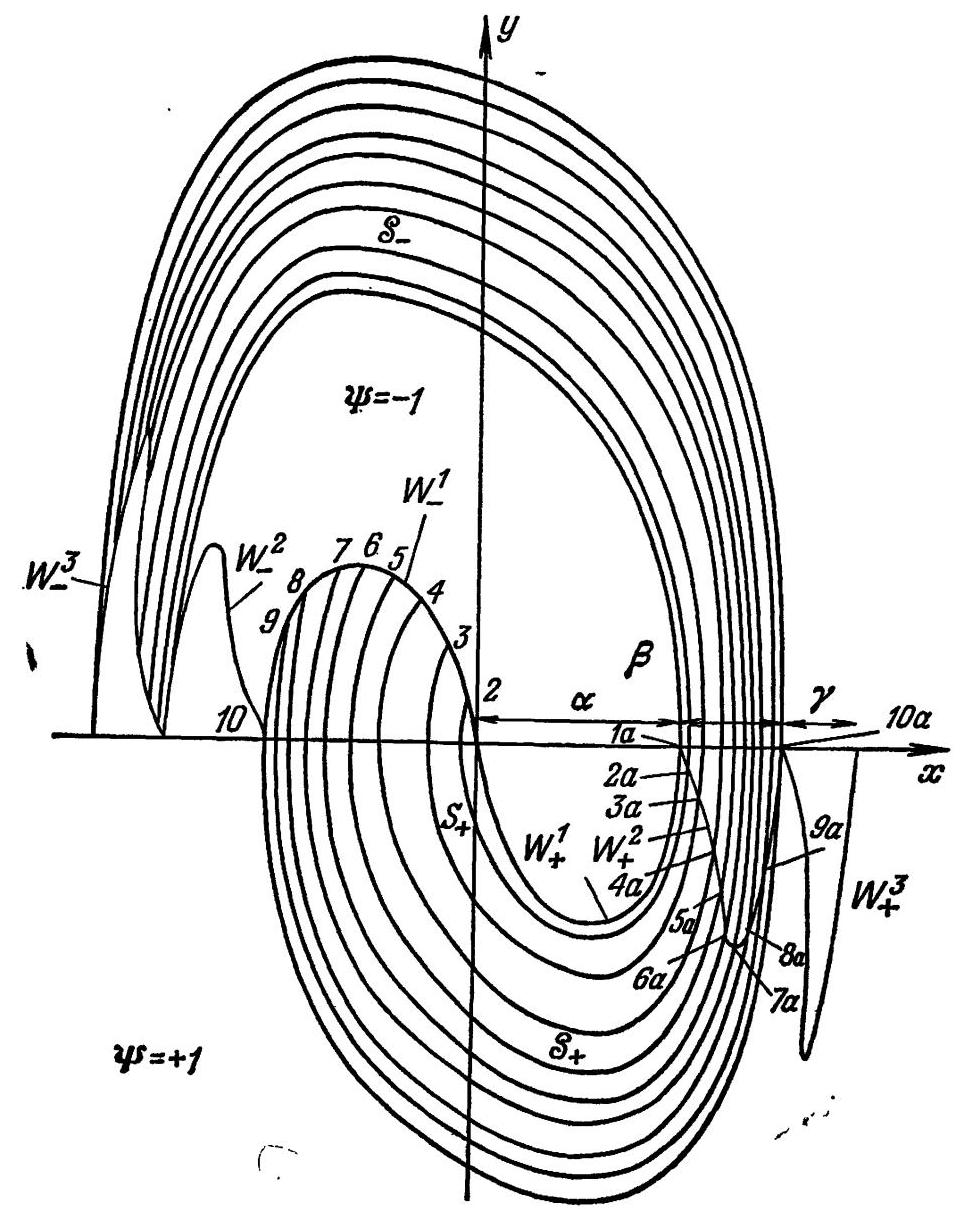
\includegraphics[max width=0.8\textwidth]{images/bo_d547k8bef24c73bgfcg0_480_358_411_964_1209_0.jpg}
\end{center}
\hspace*{3em} 

Рис. 7.5. Синтез управления с обратной связью для уравнения Дуффинга.

Tem самым,мы построили управление \(u = \Psi \left( {x,y}\right)\) с обратной связью для уравнения Дуффинга (\%). Синтез будет полным, если положить \(\Psi \left( {x,y}\right)  =  + 1\) ниже границы переключения \(W\) и \(\Psi \left( {x,y}\right)  =\) == 1 выше границы переключения W.

Возникает вопрос относительно точности, с которой мы построили кривую W на рис. 7.5 (она была построена при помощи аналого- во-цифровой вычислительной машины). Тем не менее, на рис. 7.5 видно, что линия переключения действительно является однознач- ной функцией относительно обоих потоков \$\_ и \$\_. Числен- ный метод построения управления с обратной связью, использую- ший цифровую машину, подробно рассмотрел Х. Л. Бурмейстер (H. L. Burmeister). (Cравните его рис. 3 с нашим рис. 7.5.)

Для уравнения Дуффинга с управлением

\[
\dot{x} = y
\]

\[
\dot{y} =  - x - {x}^{3} + u,
\]

где —1<ме<1, мы также построили на рис. 7.6 изохронные кривые в окрестности начала координат. Мы уже обсуждали свой- ства изохронной функции для линейной задачи оптимального быстродействия перед теоремой 21 главы 2 и в упражнении 2 раздела 5.2 для нелинейных систем. Замкнутая область, ограни- ченная каждой из этих кривых, совпадает со множеством дости- жимости из начала координат за время Т для задачи с обращен- ным временем на отрезке [0, T], где T—значение изохронной функции на соответствующей кривой. Из рис. 7.6 и рис. 7.5 видно, что множество достижимости не является выпуклым, но, по-види- мому, имеет гладкую границу.

\begin{center}
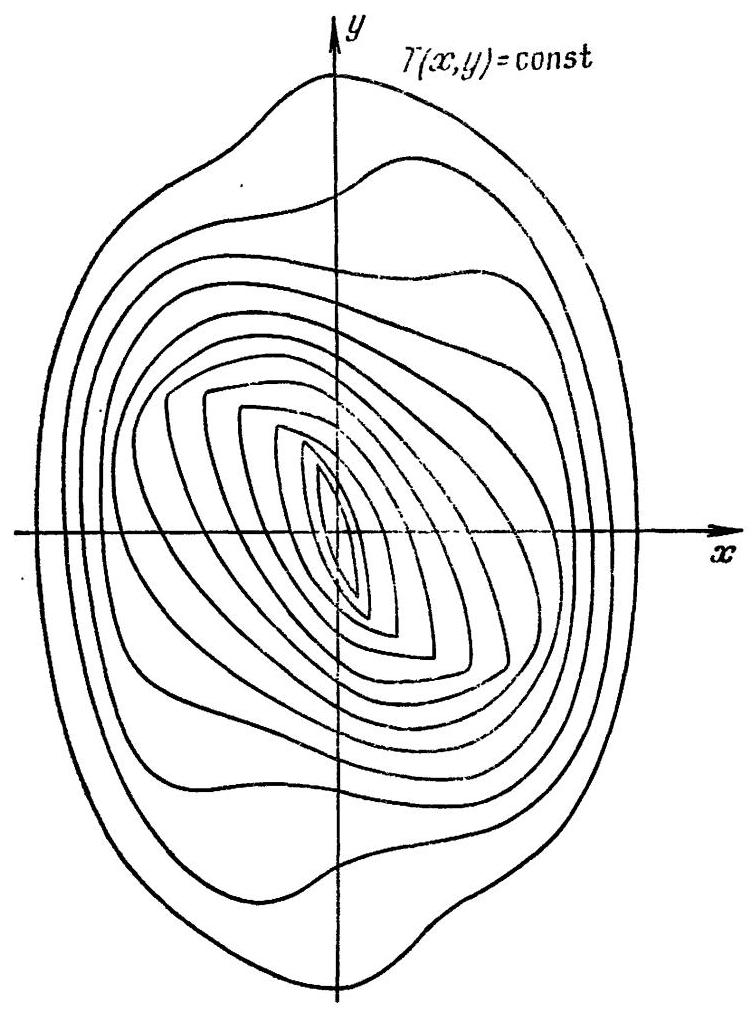
\includegraphics[max width=0.7\textwidth]{images/bo_d547k8bef24c73bgfcg0_481_379_650_753_1012_0.jpg}
\end{center}
\hspace*{3em} 

Pac. 7.6. Изохроны для системы х+х+x" и

\(\left| u\right|  \leq  1\) .

Пример 2 (маятник). Рассмотрим уравнение движения плоского маятника (рис. 7.7) массы m, подвешенного к точке опоры при помощи жесткого невесомого стержня:

\[
I\ddot{\theta } + b\dot{\theta } + {mgl}\sin \theta  = M\left( t\right) .
\]

Здесь \(I = m{l}^{2}\) — момент инерции; \(b \geq  0\) коэффициент демпфирова- ния; \(M\left( t\right)\) — внешний управляющий момент; g—rравитационная постоянная (ускорение силы тяжести); l— длина жесткого стержня маятника; m — масса, сосредо- точенная в конце жесткого стержня (см. рис. 7.7).

\begin{center}
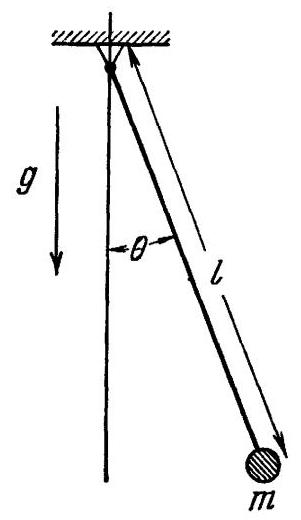
\includegraphics[max width=0.2\textwidth]{images/bo_d547k8bef24c73bgfcg0_482_237_522_301_520_0.jpg}
\end{center}
\hspace*{3em} 

Puc. 7.7., Управляе- мый маятник.

Чтобы привести уравнение к стандарт- ной форме, сделаем замену переменной \(\tau  = t\sqrt{{mgl}/I}\) и получим уравнение движения в следующем виде:

\[
\ddot{\theta } + \alpha \dot{\theta } + \sin \theta  = \beta \left( t\right) ,
\]

где \(\alpha  = b/\sqrt{\text{ Imgl }} \geq  0,\beta \left( t\right)  = M\left( t\right) /{mgl}\) . Эквива- лентная система уравнений первого порядка имеет вид

\[
\dot{\theta } = z,\;\dot{z} =  - \sin \theta  - {\alpha z} + \beta \left( t\right) .
\]

Задачей оптимального по быстродействию управления является остановка маятника в одной из точек устойчивого равновесия \(\left( {\theta  =  \pm  {2\pi k},z = 0}\right)\) ,для \(k = 0,1,2,\ldots {3a}\) минимальное время посредством выбора управляющего момента β (t), удовлетворяю- щего ограничению \(\left| {\beta \left( t\right) }\right|  \leq  B,B > 0\) . Таким образом, целевое множество \(G\) имеет вид

\[
G = \{ \left( {\theta ,z}\right)  \mid  \theta  =  \pm  {2\pi k},z = 0,k = 0,1,2,\ldots \} .
\]

Сначала покажем, что применением некоторого допустимого управ- ления из каждой начальной точки плоскости \(\left( {\theta ,z}\right)\) система может быть переведена в G. Действительно, для этого достаточно при- менить следующую последовательность управлений:

1. \(\beta \left( t\right)  =  - B\operatorname{sgn}z\left( t\right)\) до тех пор, пока система не попадет в точку с координатами \(z = 0,\theta\) ,где \({2\pi k} \leq  \theta  \leq  2\left( {k + 1}\right) \pi\) для некоторого \(k = 0,1,2,\ldots\)

2. \(\dot{\beta }\left( t\right)  =  - {\beta }_{0}z\left( t\right)\) , где \({\beta }_{0} > 0\) является настолько малым, что \(B \geq  \left| {\beta \left( t\right) }\right|\) (после вывода системы из состояния неустойчивого равновесия, если это окажется необходимым).

3. Когда исходная система попадает в окрестность точки \(\theta  = {2k\pi },z = 0\) ,мы применим критерий управляемости (глава 6) для системы

\[
\dot{\theta } = z,\;\dot{z} =  - \theta  - {\alpha z} + \beta \left( t\right)
\]

с матрицей

\[
\left\lbrack  \begin{array}{lll} 0 & 0 & 1 \\  1 &  - 1 &  - \alpha  \end{array}\right\rbrack  \left\lbrack  \begin{array}{l} 0 \\  1 \end{array}\right\rbrack  ,
\]

неособой для всех α. Это обеспечивает возможность точного дости- жения точки равновесия в течение конечного времени из любой точки некоторой окрестности положения равновесия.

Покажем теперь, произведя оценку скорости фазовой точки, что целевое множество для этой задачи можно считать компакт- ным. Тем самым, исходя из соображений непрерывности, его можно считать просто конечным. Имеем

\[
\left| \dot{z}\right|  \leq  1 + \alpha \left| z\right|  + B
\]

\[
\left| {z\left( t\right) }\right|  \leq  c{e}^{\gamma t}\text{ для некоторых }c > 0,\gamma  > 0
\]

H

\[
\left| {\theta \left( t\right) }\right|  \leq  {c}_{1}{e}^{\gamma t}\text{ для некоторого }{c}_{1} > 0\;\left( {0 \leq  t < \infty }\right) .
\]

Таким образом, решение является равномерно ограниченным на любом конечном отрезке времени. Заметим, что точки θ = 2πk, \(z = 0\) для больших |k| можно достичь лишь за очень длительный промежуток времени, и поэтому она не является кандидатом в концевые точки траектории, оптимальной по быстродействию.

Согласно теоремам главы 4 оптимальное управление 8* (t) су- ществует. Кроме того, из предшествующих результатов этого раз- дела вытекает, что оптимальное управление есть релейное управ- ление, принимающее только два значения, +B и —В, на различных интервалах времени. Здесь можно также применить предшествую- щие результаты этого раздела, касающиеся геометрии линии переключения. Приступим к построению линии переключения оптимального управления. Для удобства мы изучим сначала слу- чай, когда α=0, и затем покажем, что для случая α>0 резуль- таты выглядят даже проще.

\(\Pi\) ри \(\alpha  = 0\) каждую целевую точку можно достичь, т. е. маят- ник может быть приведен в колебательное движение все с большей и большей амплитудой, даже если В очень мало, до тех пор, пока маятник пройдет через точку неустойчивого равновесия, из кото- рой можно перейти к любым другим точкам равновесия. Мы сначала рассмотрим оптимальный переход только к одной точке равновесия, в качестве которой возьмем начало координат.

Имеется два особенно интересных случая: (1) случай, когда \(B > 2/\pi\) , который соответствует ситуации, когда линия переклю- чения (для одной целевой точки) пересекает ось 0 только в начале координат; (2) случай \(B \leq  2/\pi  -\) когда линия переключения пере- секает ось о больше, чем в одной точке.

Рассмотрим гамильтонову систему уравнений (как и в главе 5):

\[
\dot{{\eta }_{1}} =  - \frac{\partial H}{\partial \theta } = \left( {\cos \theta }\right) {\eta }_{2},\;\dot{{\eta }_{2}} =  - \frac{\partial H}{\partial z} = \alpha {\eta }_{2} - {\eta }_{1},
\]

\[
\dot{\theta } = \frac{\partial H}{\partial {\eta }_{1}} = z,\;\dot{z} = \frac{\partial H}{\partial {\eta }_{2}} =  - \sin \theta  - {\alpha z} + \beta \left( t\right) ,
\]

где

\[
H = H\left( {{\eta }_{1},{\eta }_{2},\theta ,z,\beta }\right)  = {\eta }_{1}z + {\eta }_{2}\left\lbrack  {-\sin \theta  - {\alpha z} + \beta }\right\rbrack  .
\]

Оптимальное управление является релейным максимальным управ- лением вида

\[
\beta \left( t\right)  = \operatorname{sgn}{\eta }_{2}\left( t\right) .
\]

Вопрос о том, пересекает ли линия переключения ось о более, чем в одной точке, эквивалентен вопросу о том, имеет ли более одного нуля функция η, 2(t), когда фазовая точка системы дви- жется в плоскости (θ, z) из начала координат в направлении, противоположном ходу времени вдоль траектории системы, удов- летворяющей начальным условиям \(\theta \left( 0\right)  = z\left( 0\right)  = {\eta }_{2}\left( 0\right)  = 0,{\eta }_{1}\left( 0\right)  = 1\) .

Из предшествующих результатов следует, что нули функций \({\eta }_{2}\left( t\right)\) и z \(\left( t\right)\) вдоль такой траектории чередуются. Для специаль- ных начальных условий \(\left( {0,0, \pm  1,0}\right)  = \left( {\theta \left( 0\right) ,z\left( 0\right) ,{\eta }_{1}\left( 0\right) ,{\eta }_{2}\left( 0\right) }\right)\) нули функций \({\eta }_{2}\left( t\right)\) и \(z\left( t\right)\) совпадают. Уравнения движения с обращенным временем имеют вид

\[
\dot{\theta } =  - z,\;\dot{z} = \sin \theta  - B\operatorname{sgn}{\eta }_{2},
\]

\[
\dot{{\eta }_{1}} =  - {\eta }_{2}\cos \theta ,\dot{{\eta }_{2}} = {\eta }_{1}
\]

с начальными условиями (0, 0, 1, 0) (или (0, 0, -1, 0)). Здесь функция \({\eta }_{2}\left( t\right)\) не может иметь других нулей, кроме тех, что имеет функция z (t). Рассмотрим фазовую кривую на фазовой плоскости первых двух координат, когда η, (н) с 0, т. е. кривую, удовлетворяющую уравнению

\[
\frac{dz}{d\theta } = \frac{\sin \theta  - B}{-z}
\]

проходящую через начало координат, и лежащую в четвертом квадранте. Интегрирование дает

\[
z =  - \sqrt{2\left( {\cos \theta  + {B\theta } - 1}\right) }.
\]

Эта кривая изображена на рис. 7.8 для различных значений В и, понятно, она не пересекает ось 0, если 8 >2/π и является частью кривой переключения, именно кривой \({W}_{ + }^{1}\) . Для того чтобы определить, имеет ли линия переключения ветви, смыкающиеся на бесконечности, достаточно выполнить процедуру, описанную ранее. Именно, из точки кривой \({W}_{ + }^{1}\left( {{\eta }_{1}\left( 0\right)  =  - 1,{\eta }_{2}\left( 0\right)  = 0}\right)\) мы следуем вперед во времени вдоль решений уравнений собращен- ным временем до тех пор, пока функция \({\eta }_{2}\left( t\right)\) не обратится снова в нуль, и отмечаем эту точку в плоскости (θ, z) (она принадлежит линии переключения). На рис. 7.9 построена линия переключения для случая \(\alpha  = 0,B = 1,\) причем при построении, произведенном ана- логично тому, как это было сде- лано в примере 1, использовано десять точек кривой \({W}_{ + }^{1}\) .

\begin{center}
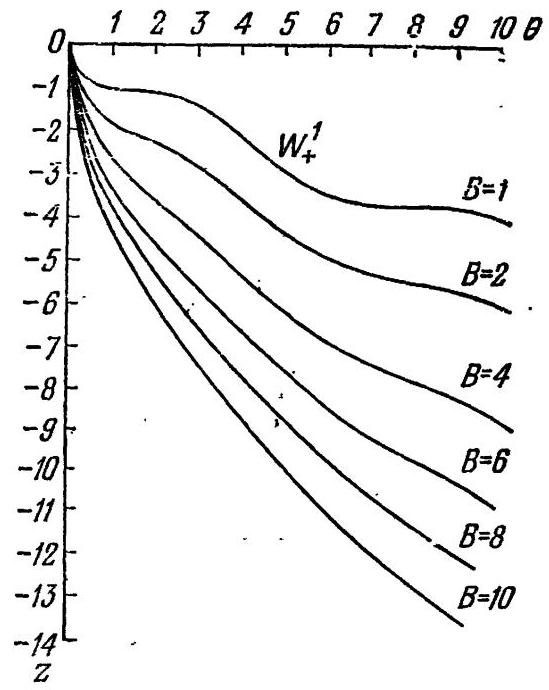
\includegraphics[max width=0.5\textwidth]{images/bo_d547k8bef24c73bgfcg0_485_876_302_549_690_0.jpg}
\end{center}
\hspace*{3em} 

Рис. 7.8. Кривая переключения для маятника при отсутствии демпфиро- вания.

Ветвь линии переключения, ле- жашую во втором квадранте, можно получить отражением построенной кривой относительно начала коор- динат. Аналогично строится линия переключения для произвольной целевой точки, являющейся концом некоторой оптимальной траектории.

Однако мы должны еще уста- новить аналогичную процедуру, которая годилась бы для всей со- вокупности целевых точек одно- временно. Покажем, что требуется рассмотреть только линию переключения слева или линию пере- ключения справа от начальной точки при решении вопроса, ка- кая точка берется в качестве целевой, если линия переключения не имеет ветвей, смыкающихся на бесконечносги. Ситуация указана на рис. 7.10 для всех кривых переключения.

\begin{center}
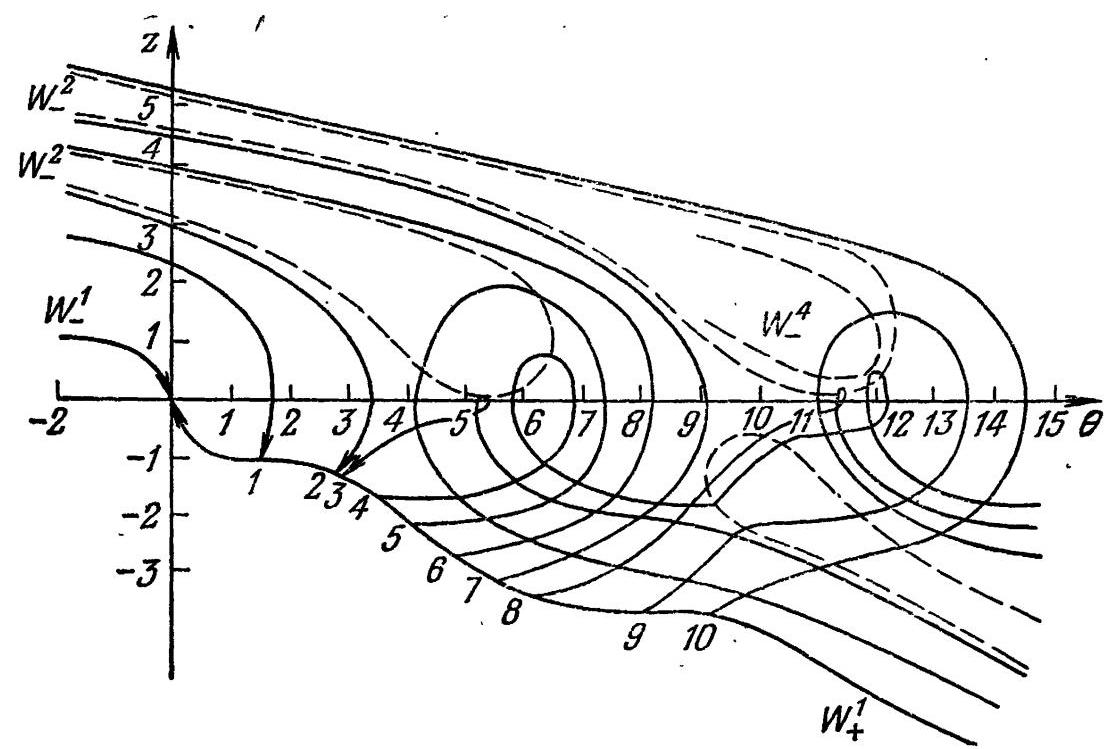
\includegraphics[max width=1.0\textwidth]{images/bo_d547k8bef24c73bgfcg0_485_240_1166_1118_749_0.jpg}
\end{center}
\hspace*{3em} 

Рис. 7.9. Построение кривой переключения для маятника в случае больших ограничений на управления.

Рассмотрим точку р на рис. 7.10. Если сначала выбрано управ- ление \(\beta  \equiv   + B\) , то может не быть переключений до тех пор, пока траектория не достигнет одной из точек а, б и т. д., т. е. пока траектория не пересечет один из кусков линии переключения. Очевидно, что переключение в точке а и последующее движение в начало координат предпочтительнее, чем переключение в точке b и движение из нее в начало координат. Это верно потому, что движение из точки а’ в точку 0 вдоль пути, проходящего через точку а’ при β≡+ В, занимает меньше времени, чем движение по пути от точки а к точке b и затем к точке 0, и, таким обра- 30м, путь от точки а к 0 занимает меньше времени, чем путь от точки а к точке b и затем в точку 0,. Аналогично, если в вна- чале выбрано равным —В, переключение происходит в точке пе- ресечения с первой кривой переключения. Полное построение синтеза оптимального управления с обратной связью показано на рис. 7.11, где пунктирная кривая найдена с помощью только что проделанного рассуждения и определяет равные по времени пути перевода системы в точку с наименьшей угловой координатой.

\begin{center}
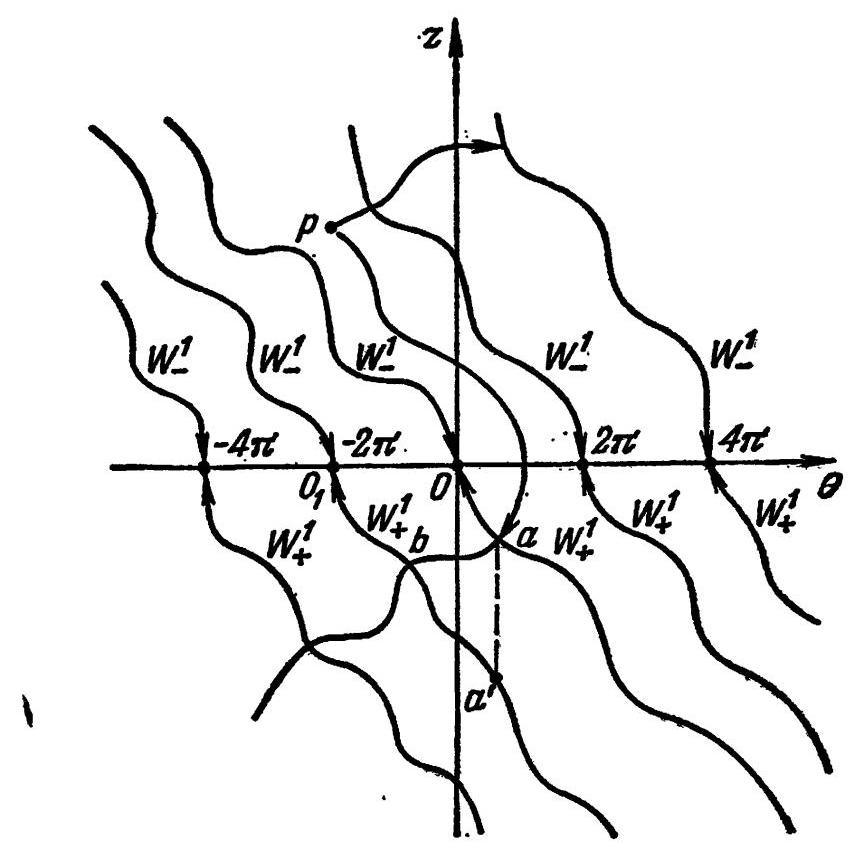
\includegraphics[max width=0.7\textwidth]{images/bo_d547k8bef24c73bgfcg0_486_352_366_860_849_0.jpg}
\end{center}
\hspace*{3em} 

Рис. 7.10. Построение управления с обратной связью для маятника.

Если а >0, то наклон кривых переключения будет круче, а способ построения аналогичен способу построения для случая \(\alpha  = 0\) . В самом деле, легко показать, что если α> 2, то линия

переключения не имеет кусков ветвей, смыкающихся на бесконеч. ности. Мы должны лишь показать, что решения уравнения

\[
{\ddot{\eta }}_{2} + \alpha {\dot{\eta }}_{2} + {\eta }_{2}\left( {\cos \theta \left( t\right) }\right)  = 0
\]

имеют не более одного нуля. Сделаем замену переменного \({\eta }_{2} = {e}^{-\left( {\alpha /2}\right) t}v\) . Получим уравнение относительно \(v\) :

\[
\ddot{v} + v\left( {-\frac{{\alpha }^{2}}{4} + \cos \theta \left( t\right) }\right)  = 0.
\]

Решения этого уравнения при \(\alpha  > 2\) имеют не более одного действительного нуля. Линия переключений и синтез управления с обратной связью для \(\alpha  = 3,B = 1\) показаны на рис. 7.12.

\begin{center}
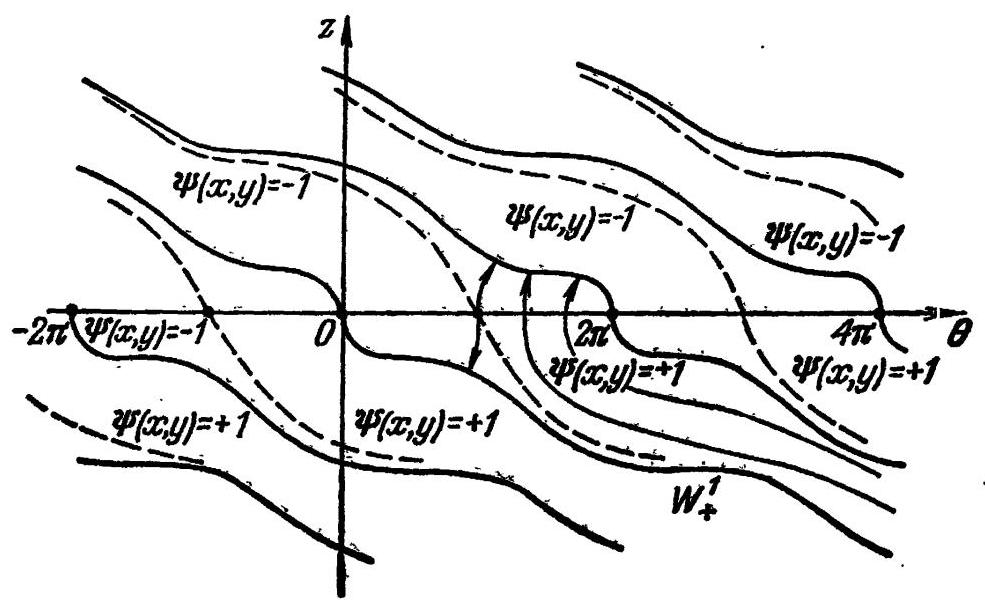
\includegraphics[max width=0.9\textwidth]{images/bo_d547k8bef24c73bgfcg0_487_327_662_985_600_0.jpg}
\end{center}
\hspace*{3em} 

Рнс. 7.11. Сннтез управлення с обратной связыюдля маятннка.

\begin{center}
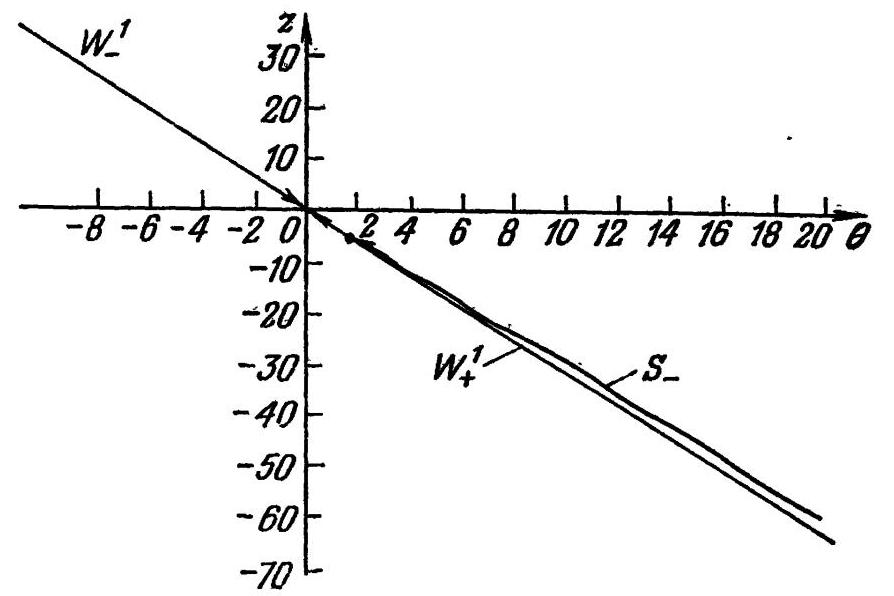
\includegraphics[max width=0.8\textwidth]{images/bo_d547k8bef24c73bgfcg0_487_366_1340_894_596_0.jpg}
\end{center}
\hspace*{3em} 

Рис. 7.12. Кривая переключения для маятника в случае B=1, α=8.

Рассмотрим, наконец, случай, когда \(B \leq  2/\pi\) , а α≥0. При \(B = 0,1\mathrm{\pi }\alpha  = 0\) линия переключения для задачи перевода системы в начало координат строится как в предыдущем примере, и пока- зана на рис 7.13. Эта же процедура годится и для нахождения линии переключения при а >0.

\begin{center}
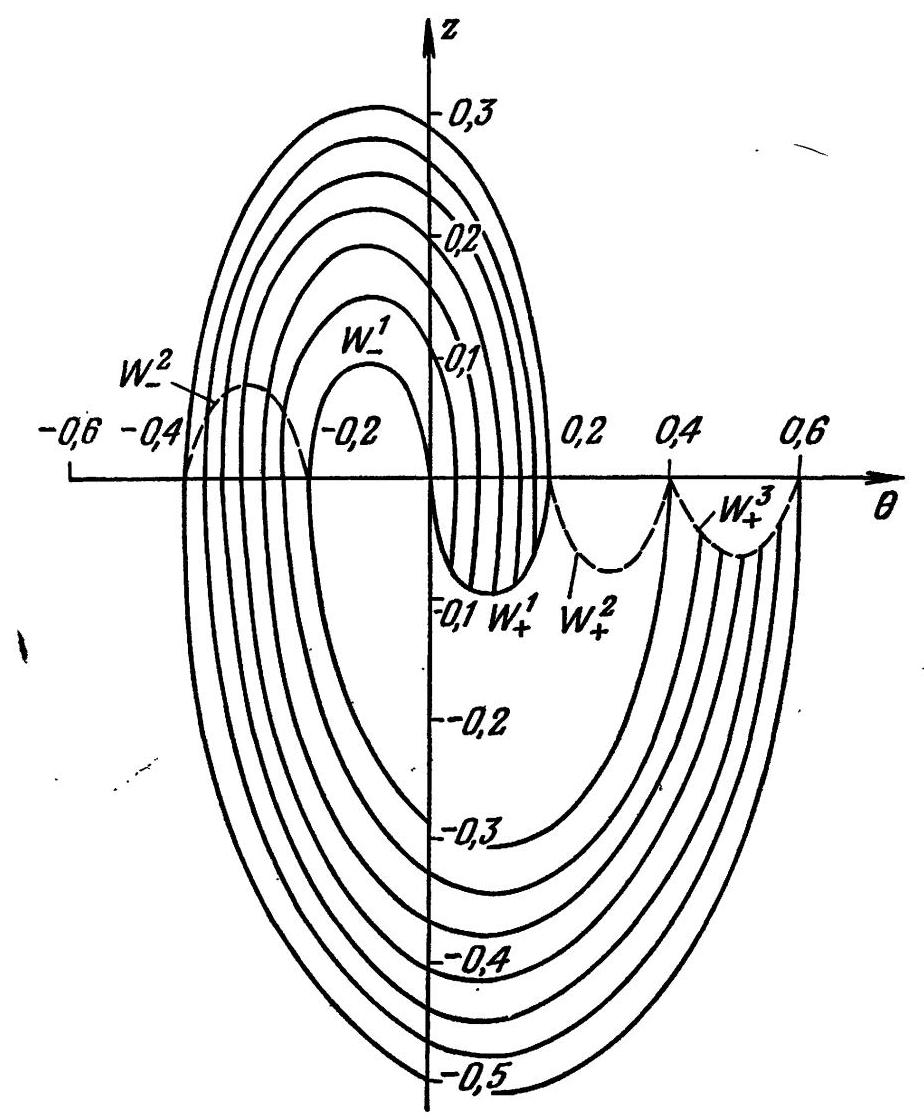
\includegraphics[max width=0.8\textwidth]{images/bo_d547k8bef24c73bgfcg0_488_354_428_924_1119_0.jpg}
\end{center}
\hspace*{3em} 

Рис. 7.13. Крявая переключения для маятника в случае B=0,1, a=0.

Вообще, интересно заметить, что фазовое пространство для маятника является цилиндром, если все точки устойчивого равно- весия считать эквивалентными. Задача оптимального быстродейст- вия, таким образом, должна решаться в фазовом пространстве, которое топологически отлично от плоскости, и это топологическое несоответствие является причиной чрезмерной сложности линии переключения.

\section*{Упражнения}

1. Найти область нуль-управляемости для системы

\[
\dot{x} = {y}^{3},
\]

\[
\dot{y} = u,\;\left| u\right|  \leq  1.
\]

2. На рисунке 7.5 мы обозначили расстояния между последовательными точками, в которых линия переключения пересекает ось х через α, β, γ, соот- вестственно, в порядке возрастания абсцисс точек пересечения (см. рис. 7.5). Пля уравнения Дуффинга (в примере 1 а ≥ β ≥ γ) доказать, что расстояние между двумя последовательными точками пересечения вообще убывает с ростом их абсцисс (для этого примера) и что оно стремится к нулю при х — о.

3. Построить кривую переключения для уравнения Дуффинга с управле- нием и демпфированием:

\[
\dot{x} = y,\;\dot{y} =  - x - {x}^{3} - y + u,\;\left| u\right|  \leq  1
\]

(см. пример 1 и рис. 7.5).

\section*{7.2. Оптимальное управление метеорологической ракетой}

В 1919 г. Годдар рассмотрел задачу о подъеме летательного аппарата с реактивным двигателем на заданную высоту над зем- лей при минимальном расходе топлива. Он установил, что эта задача не может быть решена обычными методами вариационного исчисления. Эта задача эквивалентна задаче максимизации высоты подъема аппарата с заранее заданными топливными ресурсами. Мы рассмотрим этот вариант задачи для случая, когда сила тяги двигателя ракеты ограничена по величине, и примем обычную математическую модель для описания силы лобового сопротивле- ния. Случай, когда ограничения на силу тяги заранее не нало- жены, был исследован Эвингом (Ewing) и сведён к задаче с огра- ничением на силу тяги путем введения некоторого равномерного условия Липшица. Надо иметь в виду, что в практических зада- чах сила тяги всегда ограничена.

Мы исследуем систему уравнений

\[
\left( {\mathcal{S}}_{0}\right)
\]

\[
\frac{dh}{dt} = v,\;\frac{dv}{dt} = \frac{T - D\left( {v,h}\right) }{m} - {c}_{1},\;\frac{dm}{dt} =  - \frac{T}{{c}_{2}},
\]

где h есть высота летательного аппарата над землей, v-его вер- тикальная скорость, m-ero масса, а \({c}_{1}\) и \({c}_{2}\) —положительные константы. Управление Т есть сила тяги ракеты, которая может изменяться в границах 0≤ \(T \leq  {T}_{1}\) , a \(D\left( {v,h}\right)\) —лобовое сопротив- ление, определенное для \(h \geq  0\) и удовлетворяющее условиям:

1) \(D\left( {0,h}\right)  = 0\) .

2) \(\left| {D\left( {v,{h}_{1}}\right) }\right|  > \left| {D\left( {v,{h}_{2}}\right) }\right|\) , если \({h}_{2} > {h}_{1}\) .

3) \(- D\left( {-v,h}\right)  = D\left( {v,h}\right)  \geq  0\) , если \(v \geq  0\) .

4) \(D\left( {v,h}\right)  \rightarrow  0\) при \(h \rightarrow  \infty\) для всех v.

5) \(D\left( {v,h}\right)  \in  {C}^{1}\) .

6) \({vD}\left( {v,h}\right)  \geq  0\) .

7) \(\left| {D\left( {{v}_{1},h}\right) }\right|  \geq  \left| {D\left( {{v}_{2},h}\right) }\right|\) , если \(\left| {v}_{1}\right|  \geq  \left| {v}_{2}\right|\) .

Лобовое сопротивление как функция v и h задается приближенно формулой \(D = v\left| v\right| {e}^{-{\alpha h}}\) ,где α = const \(> 0\) . Macca \(m\) в начальный момент равна \({m}_{0}\) , a затем уменьшается до \({m}_{1} > 0\) вследствие рас- хода топлива. Система с более точной формулой для лобово- го сопротивления может быть исследована примерно теми же методами, которые Эвинг применил для случая, когда лобовое сопротивление задается формулой

\[
D = v\left| v\right| {e}^{-{\alpha h}}.
\]

В последнее время были исследованы некоторые новые аспекты этой задачи (см. [Лоуден]).

Предполагается, что имеется момент времени те ОО С 4 с 2 см), до которого эксперимент должен (быть закончен и поэтому мы рас- смотрим только задачи максимизации высоты для моментов времени меньших или равных т. Задача состоит в том, чтобы в классе допустимых управлений найти управляющую функцию \(T\left( t\right)\) (опре- деленную на интервале [0, t, 1 и удовлетворяющую ограничениям \(0 \leq  T \leq  {T}_{1}\) ) так,чтобы первая координата \(h\left( t\right)\) соответствующего решения (h(t), v(t), m(t)) системы с начальными условиями \(\left( {0,0,{m}_{0}}\right)\) в момент \({t}_{1} \leq  \bar{t}\) достигала бы максимального возможного значения \(h\left( {t}_{1}\right)\) , a caмо решение удовлетворяло фазовым ограниче- ниям: \({m}_{1} \leq  m\left( t\right)  \leq  {m}_{0},h\left( t\right)  \geq  0\) .

Мы займемся сначала вопросом о существовании оптимального управления, а потом воспользуемся необходимыми условиями оптимальности, найденными в главе 5. Затем мы выведем доста- точные условия оптимальности управления, а также произведем синтез оптимального управления для рассматриваемой задачи при некоторых предположениях относительно характера изменения силы лобового сопротивления.

Существование. Для того чтобы установить существование оптимальной управляющей функции нам придется изучить струк- туру замыкания множества достижимости (см. главу 4). Доказа- тельство существования получится более длинным, чем это необ- ходимо, однако некоторые из промежуточных результатов понадобятся нам в дальнейшем при обсуждении характера оптимального управления (см. упражнение 3). В ходе доказатель- ства мы воспользуемся монотонностью функции \(m\left( t\right)\) , a также учтем соответствующие ограничения. Ограничение на h будет учтено следующим образом. Сначала мы позволим величине h принимать и отрицательные значения и дадим доказательство су- шествования оптимального управления для этого случая, а затем покажем, что оптимум всегда имеет место при \(h \geq  0\) .

Предполагается, что функция \(D\left( {v,h}\right)\) определена по написан- ной выше формуле. Заменим систему у, системой

\[
\frac{dh}{dt} = v
\]

\[
\left( {\mathcal{Y}}_{1}\right)
\]

\[
\frac{dv}{dt} = F\left( M\right) \left\lbrack  {T - D\left( {v,h}\right) }\right\rbrack   - {c}_{1},
\]

\[
\frac{dM}{dt} =  - \frac{T}{{c}_{2}},
\]

где

\[
F\left( M\right)  = \left\{  \begin{array}{ll} {\left( M + {m}_{1}\right) }^{-1}, & \operatorname{ec\text{ л }\text{ и }}M \geq  0, \\  \frac{{m}_{1} - M}{{m}_{1}^{2}}, & \operatorname{ec\text{ л }\text{ и }}M < 0. \end{array}\right.
\]

\(\exists \mathrm{{ra}}\) cuc \(\mathrm{T}\) стана совпадает с системой \({\mathcal{G}}_{0}\) при \(0 \leq  M \leq  {m}_{0} - {m}_{1}\) ,т. e. при \({m}_{1} \leq  m \leq  {m}_{0}\) и на этом интервале

\[
M\left( t\right)  = m\left( t\right)  - {m}_{1}.
\]

К этой системе мы добавим еще координату х для того, чтобы учесть независимую переменную—время, и рассмотрим расши- ренную систему

\[
\frac{dx}{dt} = 1,\;\frac{dh}{dt} = v
\]

(9)
\[
\frac{dv}{dt} = F\left( M\right) \left\lbrack  {T - D\left( {v,h}\right) }\right\rbrack   - {c}_{1},\;\frac{dM}{dt} =  - \frac{T}{{c}_{2}}
\]

с начальными условиями \(x\left( 0\right)  = v\left( 0\right)  = h\left( 0\right)  = 0,M\left( 0\right)  = {m}_{0} - {m}_{1}\) .

На этот раз, не принимая во внимание приведенные выше ограниче- ния на h и M, рассмотрим множество достижимости (см. главу 4) R (i) для системы \$ в пространстве переменных (x, h, v, M). Это множе- ство является компактным в R*1, если каждое решение системы \$ является ограниченным на интервале [0, \(\bar{t}\) ].

Каждой допустимой управляющей функции \(T\left( t\right)\) ,т. е. измери- мому управлению \(T\left( t\right)\) , изменяющемуся на интервале [0, \({T}_{1}\) ], соответствует единственное ограниченное абсолютно непрерывное решение \(\left( {x\left( t\right) ,h\left( t\right) ,v\left( t\right) ,M\left( t\right) }\right)\) системы \$, y довлетворяющее на- чальным условиям (x(0), h(0), v(0), M(0)) = (0, 0,0, \({m}_{0} - {m}_{1}\) ) и определенное на интервале [0, \(\bar{t}\) ]. Oно удовлетворяет системе диф- ференциальных уравнений \$9 почти всюду на интервале [0, 1].

Ограниченность решения доказывается следующим образом. Функция М (t), соответствующая каждой допустимой управляю- щей функции \(T\left( t\right)\) , ompeделенной на интервале [0, \(\bar{t}\) ],является ограниченной, и поэтому таковой является и функция \(F\left( {M\left( t\right) }\right)\) .

Рассмотрим выражение

\[
\frac{d{\left| v/2\right| }^{2}}{dt} = v\frac{dv}{dt} = {vF}\left( M\right) \left\lbrack  {T\left( t\right)  - D\left( {v,h}\right) }\right\rbrack   - v{c}_{1},
\]

из которого следует, что

\[
\frac{d{\left| v/2\right| }^{2}}{dt} \leq  \left| v\right| \left| {F\left( M\right) T\left( t\right)  - {c}_{1}}\right|
\]

ИЛИ

\[
\frac{d\left| v\right| }{dt} \leq  \left| {F\left( M\right) T - {c}_{1}}\right| .
\]

Поэтому функция \(v\left( t\right)\) [a следовательно, и функция \(h\left( t\right)\) ] ограни- чена на конечном интервале [0, \(\bar{t}\) ].

Тем самым ограничение на \(\dot{M}\) наложено. Рассмотрим пересе- чение замкнутых множеств

\[
H = \left\{  {x,h,v,M \mid  0 \leq  x \leq  \bar{t},v\text{ и }h\text{ в }{R}^{1},0 \leq  M \leq  {m}_{0} - {m}_{1}}\right\}
\]

и \(\widehat{R}\left( \bar{t}\right)\) ,т. e. рассмотрим компактное множество

\[
\widehat{K}\left( \bar{t}\right)  = H \cap  \widehat{R}\left( \bar{t}\right) .
\]

Так как \(M\left( t\right)\) —невозрастающая функция на интервале [0, 7], то очевидно, что \(\widehat{K}\left( \overrightarrow{t}\right)\) есть множество достижимости при учете огра- ничений. Линейная функция \(\mathcal{L}\left( {x,h,v,M}\right)  \equiv  h\) на компактном множестве К (7) достигает своего минимального и максимального значения. Это доказывает существование оптимальной управляю- щей функции для случая, когда функция \(h\left( t\right)\) может принимать и отрицательные значения.

Теперь мы хотим показать, что вдоль оптимального решения скорость и высота положительны. Для этого сначала докажем лемму.

Лемма 1. Рассмотрим систему G, как и выше, с началь- ными условиями ( \({h}_{0},{v}_{0} \geq  0,{m}_{0} - {m}_{1}\) ) в момент \({t}_{0}\) . Пусть T(t) — допустимая управляющая функция с соответствующим решением \(\left( {h\left( t\right) ,v\left( t\right) ,\dot{M}\left( t\right) }\right)\) на интервале \(\left\lbrack  {{t}_{0},{t}_{1}}\right\rbrack  ,a\;v\left( t\right)  \geq  0\) на интервале \(\left\lbrack  {{t}_{0},{t}_{1}}\right\rbrack\) . Тогда для каждой начальной точки ( \(\overline{{h}_{0}},\overline{{v}_{0}},\overline{{M}_{0}}\) ), maкой, что \(\left( {\overline{{h}_{0}} \geq  {h}_{0},\overline{{v}_{0}} \geq  {v}_{0},{\bar{M}}_{0} = {m}_{0} - {m}_{1}}\right)\) , cyществует такая допустимая управляющая функция \(\bar{T}\left( t\right)\) на интервале [t, t, 1, что соответст- вующее ей решение \(\left\lbrack  {\overline{h}\left( t\right) ,\overline{v}\left( t\right) ,\bar{M}\left( t\right) }\right\rbrack\) проходит через начальную \(\operatorname{\text{ т }\text{ о }\text{ ч }\text{ к }\text{ у }}\left( {{\bar{h}}_{0},{\bar{v}}_{0},{\bar{M}}_{0}}\right)\) в момент б, и удовлетворяет условиям h(t) ≥ \(\geq  h\left( t\right) ,\bar{v}\left( t\right)  \geq  v\left( t\right)  - {при}{t}_{0} \leq  t \leq  {t}_{1}u\bar{M}\left( {t}_{1}\right)  = M\left( {t}_{1}\right)\) . Кроме moro, если \({\overrightarrow{h}}_{0} > {h}_{0}\) , mo можно добиться строгого неравенства h(t) > h(t). (Т. е. всегда есть возможность получить решение, превышающее в смысле высоты и скорости наперед заданное решение с поло- жительной скоростью, если это превышение имело место в на- чальный момент времени.)

Доказательство. Выберем \(\bar{T}\left( t\right)  = T\left( t\right)\) при \({t}_{0} \leq  t \leq  {t}_{1}\) . Тогда \(\bar{M}\left( t\right)  = M\left( t\right)\) и \(F\left( {\bar{M}\left( t\right) }\right)  = F\left( {M\left( t\right) }\right)\) всюду на интервале \(\left\lbrack  {{t}_{0},{t}_{1}}\right\rbrack\) . Так как \(D\left( {v,h}\right)  \geq  D\left( {v,\bar{h}}\right)\) при \(v \geq  0\) ,и \(\bar{h} \geq  h\) , to \(\bar{v}\left( t\right)\) не может стать меньше, чем \(v\left( t\right)\) . Но тогда и \(\bar{h}\left( t\right)\) по крайней мере не меньше, чем \(h\left( t\right)\) . Так как \(D\left( {v,h}\right)  > D\left( {v,\bar{h}}\right)\) при \(\bar{h} > h\) , то строгое неравенство также выполняется.

Из физических соображений следует, что

\[
{T}_{1} \geq  {m}_{0}{c}_{1},\;{m}_{1} < {m}_{0}.
\]

Это лает возможность показать, что даже если физическое ограни- чение на \(h\) не используется в задаче, максимальная высота h*>0, причем высоты h* можно достичь вдоль решения, скорость кото- рого все время положительна. Однако, если ты лет. рассмотрим жесткое ограничение на \(h\) и сожжем столько топлива, сколько нужно для того, чтобы масса m уменьшалась до значения, при котором \({T}_{1} = m{c}_{1} = \left( {M + {m}_{1}{c}_{1}}\right)\) , если возможно, и до тех пор, пока это значение не достигнуто, каждое управление, которое использует топливо, оптимально. Когда это значение достигнуто, задача принимает указанный выше вид, и мы тогда снимаем фа- зовое ограничение. Поэтому достаточно рассмотреть только слу- чай, когда \({T}_{1} \geq  {m}_{0}{c}_{1}\) без ограничений на h. Лемма доказана.

Теорема 10. Рассмотрим систему \$1, как и выше, с началь- ным условием \({h}_{0} = {v}_{0} = 0,{M}_{0} = {m}_{0} - {m}_{1}\) . Пусть T* (t) будет опти- мальной управляющей функцией, которой соответствует на оптимальном интервале [0, t*] решение (h*(t), v*(t), M*(t)). Тогда \({h}^{ * }\left( t\right)  \geq  0,{v}^{ * }\left( t\right)  \geq  0\) на \(\left\lbrack  {0,{t}^{ * }}\right\rbrack  ,a{T}^{ * }\left( t\right)\) ecm o nтимальное управле- ние, удовлетворяющее всем ограничениям.

Доказательство. Если \({m}_{1} = {m}_{0}\) ,т. e. топлива нет, опти- мальная высота h*=0. При этом также t*=0. Если ты с то, то \({h}^{ * } > 0\) ,и ясно,что \({t}^{ * } > 0\) . Так как \({h}^{ * }\left( {t}^{ * }\right)  > 0\) , To \(v\left( {t}^{ * }\right)  \geq  0\) , Td \({v}^{ * }\left( t\right)\) - абсолютно непрерывное решение на интервале [0, \({t}^{ * }\) ].

Предположим, что \({v}^{ * }\left( t\right)  < 0\) на некотором подынтервале поло- жительной длины из интервала [0, \({t}^{ * }\) ], \(u\) пусть \({t}_{2}u{t}_{3} - \kappa\) онцевые точки этого интервала, т. е. \({v}^{ * }\left( t\right)  < 0\) при \(t \in  \left( {{t}_{2},{t}_{3}}\right) ;{v}^{ * }\left( {t}_{2}\right)  = \; = {v}^{ * }\left( {t}_{3}\right)  = 0\) , a \({v}^{ * }\left( t\right)  \geq  0\) nput \(t \in  \left\lbrack  {{t}_{3},{t}^{ * }}\right\rbrack\) . Ясно,что \({M}^{ * }\left( {t}_{2}\right)  \geq  {M}^{ * }\left( {t}_{3}\right)  \geq  0\) .

Так \(\kappa\) ax \({v}^{ * }\left( t\right)  < 0\) на интервале \(\left( {{t}_{2},{t}_{3}}\right)\) , to \({h}^{ * }\left( {t}_{3}\right)  < {h}^{ * }\left( {t}_{2}\right)\) . Пусть \({M}^{ * }\left( {t}_{2}\right)  - {M}^{ * }\left( {t}_{3}\right)  = \beta\) . B точке \(\left( {{h}^{ * }\left( {t}_{2}\right) ,{v}^{ * }\left( {t}_{2}\right)  = 0}\right.\) , \(\left. {{M}^{ * }\left( {t}_{2}\right) }\right)\) выберем управляющую функцию \(T\left( t\right)  = {T}_{1}\) для интервала времени \(\left\lbrack  {{t}_{2},{\bar{t}}_{3}}\right\rbrack\) такой длины,чтобы \(\left( {{T}_{1}/{c}_{2}}\right) \left( {{\bar{t}}_{3} - {t}_{2}}\right)  = \beta\) . Oчевидно,что \(\overline{{t}_{3}} \leq  {t}_{3},\;v\left( \overline{{t}_{3}}\right)  > 0,\;h\left( \overline{{t}_{3}}\right)  \geq  {h}^{ * }\left( {t}_{2}\right)  \geq  {h}^{ * }\left( {t}_{3}\right) \;\mathrm{u}\;M\left( \overline{{t}_{3}}\right)  = M\left( {t}_{3}\right) .\;\mathrm{{На}}\) интервале \(\left\lbrack  {{\bar{t}}_{3},{t}^{ * } - \left( {{t}_{3} - {\bar{t}}_{3}}\right) }\right\rbrack\) выберем управление \(T\left( t\right)\) таким же, как и в доказательстве леммы, с соответствующим сдвигом во времени. Так как \({v}^{ * }\left( t\right)  \geq  0\) на интервале [i, t’*], \(v\left( t\right)  \geq  0\) на интервале \(\left\lbrack  {{t}_{3},{t}_{1}}\right\rbrack  ,\left( {{t}_{1} = {t}^{ * } - \left( {{t}_{3} - {t}_{3}}\right) }\right)\) , то как и в лемме 1 находим, что \(h\left( {t}_{1}\right)  > {h}^{ * }\left( {t}^{ * }\right) ,{t}_{1} \leq  {t}^{ * }\) ,что противоречит оптимальности управ- ления \({T}^{ * }\left( t\right)\) . Теорема доказана.

\section*{Необходимые и достаточные условия оптимальности управления}

Теперь сформулируем задачу в стандартной форме с тем, чтобы мы могли воспользоваться результатами главы 5 относительно необходимых условий оптимальности. Различные свойства опти- мального управления будут описаны ниже.

Рассмотрим систему

\[
\text{ (F) }\frac{dh}{dt} = v,\frac{dv}{dt} = \frac{T - {D}_{0}\left( v\right) {e}^{-{\alpha h}}}{m} - {c}_{1},\frac{dm}{dt} =  - \frac{T}{{c}_{2}},\;0 \leq  T \leq  {T}_{1}\text{ , }
\]

где предполагается, что лобовое сопротивление имеет вид Ло (о) еме \(\left( {{D}_{0}\left( v\right)  \in  {C}^{2}}\right)\) ,и,кроме того, удовлетворяет условиям 1) и 7) пре- дыдущего раздела. В дальнейшем мы предположим также, что:

8) \(v\left\lbrack  {\frac{{\partial }^{2}{D}_{0}}{\partial {v}^{2}} + \frac{1}{{c}_{2}}\frac{\partial {D}_{0}}{\partial v}}\right\rbrack   + \frac{{D}_{0}}{{c}_{2}} > 0\;n\) pu \(v > 0;\alpha ,{c}_{1}u{c}_{2} - n\) oложи- тельные постоянные. Мы выбираем начальные условия \(h\left( 0\right)  = \; = v\left( 0\right)  = 0,m\left( 0\right)  = {m}_{0}\) и накладываем ограничения \(h \geq  0,v \geq  0\) , \(0 < {m}_{1} \leq  m \leq  {m}_{0}\) . Предполагается, наконец, что \({T}_{1} > {m}_{0}{c}_{1}\) (см. рассуждения, предшествующие теореме 10).

Выпишем соответствующую функцию Гамильтона (см. главу 5)

\[
H\left( {{\eta }_{1},{\eta }_{2},{\eta }_{3},h,v,m,T}\right)  = {\eta }_{1}v + {\eta }_{2}\left\lbrack  {\frac{T - {D}_{0}\left( v\right) {e}^{-{\alpha h}}}{m} - {c}_{1}}\right\rbrack   + {\eta }_{3}\left\lbrack  {-\frac{T}{{c}_{2}}}\right\rbrack  .
\]

Сопряженная система дифференциальных уравнений имеет вид

\[
{\dot{\eta }}_{1} =  - {\eta }_{2}\frac{\alpha }{m}{D}_{0}\left( v\right) {e}^{-{\alpha h}},
\]

(A)
\[
\dot{{\eta }_{2}} =  - {\eta }_{1} + {\eta }_{2}\frac{\partial {D}_{0}\left( v\right) }{\partial v}\frac{{e}^{-{\alpha h}}}{m},
\]

\[
\dot{{\eta }_{3}} = {\eta }_{2}\frac{1}{{m}^{2}}\left\lbrack  {T - {D}_{0}\left( v\right) {e}^{-{\alpha h}}}\right\rbrack  .
\]

Пусть и в тремя, за которое достигается максимальная высота. Тогда имеют место следующие граничные условия (см. главу 5): \({\eta }_{1}\left( {t}_{1}\right)  \geq  0,{\eta }_{2}\left( {t}_{1}\right)  = 0,{\eta }_{3}\left( {t}_{1}\right)  \geq  0,m\left( {t}_{1}\right)  \geq  {m}_{1},v\left( {t}_{1}\right)  \geq  0,h\left( {t}_{1}\right)  \geq  0.\)

Определим функцию переключения по формуле

\[
W = \left\lbrack  {{\eta }_{2}\frac{1}{m} - {\eta }_{3}\frac{1}{{c}_{2}}}\right\rbrack  .
\]

Из принципа максимума следует, что если Т(t) есть максималь- ная управляющая функция на интервале [0, t], то для почти всех t из интервала [0, \({t}_{1}\rbrack ,\left( {{t}_{1} \leq  \bar{t}}\right)\) ,

\(T\left( t\right)  = {T}_{1}\) , если \(W\left( t\right)  > 0,\;T\left( t\right)  = 0\) , если \(W\left( t\right)  < 0,\)

\[
0 \leq  T\left( t\right)  \leq  {T}_{1},\operatorname{ec\text{ л }\text{ и }}W\left( t\right)  = 0.
\]

Подынтервал [ξ1, ξ2] интервала [0, tˈ1], на котором максимальное управление \(T\left( t\right)\) равно нулю,мы будем называть интервалом \(\partial {pe}\breve{u}{\phi a}\) ; если \(W\left( t\right)  > 0\) на \(\left\lbrack  {{\xi }_{1},{\xi }_{2}}\right\rbrack\) , To мы назовем \(\left\lbrack  {{\xi }_{1},{\xi }_{2}}\right\rbrack\) интерва- лом полной тяги; и, наконец, интервал, на котором W ≡ 0, будем называть интервалом переменной тяги. Отметим, что W (t) есть сумма некоторого числа абсолютно непрерывных функций. Кроме roro, \(H \equiv  0\) Bдоль максимального рещеня \(\left( {h\left( t\right) ,v\left( t\right) ,m\left( t\right) }\right)\) ,

\(t \in  \left\lbrack  {0,{t}_{1}}\right\rbrack\) ,и не обращающееся в нуль решение сопряженной си- стемы является абсолютно непрерывным на интервале [0, \({t}_{1}\) ].

Обозначим для удобства

\[
E = \left\lbrack  {v\frac{\partial {D}_{0}}{\partial v} + \frac{{D}_{0}v}{{c}_{2}} - {D}_{0}}\right\rbrack  {e}^{-{\alpha h}} - m{c}_{1} = \lambda \left( v\right) {e}^{-{\alpha h}} - m{c}_{1},
\]

где

\[
\lambda \left( v\right)  = \left\lbrack  {v\frac{\partial {D}_{0}}{\partial v} + \frac{{D}_{0}v}{{c}_{2}} - {D}_{0}}\right\rbrack  .
\]

Отметим, что условие 8) для силы лобового сопротивления тогда принимает вид

\[
\frac{d\lambda }{dv} > 0\;\text{ при }\;v > 0.
\]

Далее, \(\lambda \left( 0\right)  = 0\) , raK \(\;\operatorname{qro}\;\lambda \left( v\right)  > 0\;\) при \(\;v > 0\) .

Теорема 11. Рассмотрим систему Ф, удовлетворяющую усло- виям 1) — 8) предыдущего раздела с начальными условиями h (0) = \(= v\left( 0\right)  = 0,m\left( 0\right)  = {m}_{0}\) . Пусть T (t) (0 ≤ t ≤ t,1) есть оптимальная управляющая функция, которой соответствует решение (h (t), v (t), \(m\left( t\right) )\) , \(y\) does \(n\) express the case of the limit the number of limits of the limit is not existing the limit of the limit is on the limit of the limit on the limit of the limit. \(\geq  m\left( t\right)  \geq  {m}_{1}\left( {0 \leq  t \leq  {t}_{1}}\right)\) . Тогда cyluecтвует ε \(> 0\) такое, что \(W\left( t\right)  > 0\) для \(t \in  \left( {0,\mathrm{\varepsilon }}\right)\) , m. e. интервал управления начинается с интервала полной тяги.

Доказательство. Для того чтобы скорость и высота оста- вались положительными (при \({T}_{1} > {m}_{0}{c}_{1}\) ) для \(t \in  \left\lbrack  {0,{t}_{1}}\right\rbrack\) необходимо, чтобы оптимальное управление было строго положительным \(\left( {T\left( t\right)  > 0}\right)\) на некотором компактном подмножестве T\_, положитель- ной меры из интервала [0, ε1] для малого в 1.0.

Допустим, что \(W\left( t\right)  \equiv  0\) на \(\left\lbrack  {0,{\varepsilon }_{2}}\right\rbrack\) для некоторого \({\varepsilon }_{2} > 0\) . Тогда \(\frac{dW}{dt} \equiv  0\) на \(\left\lbrack  {0,{\varepsilon }_{2}}\right\rbrack\) (вычисляем производную на внутренней части интервала), т. е.

\[
- \frac{1}{m}{\eta }_{1} + {\eta }_{2}\frac{1}{{m}^{2}}\left\lbrack  {\frac{\partial {D}_{0}}{\partial v}{e}^{-{\alpha h}} + \frac{{D}_{0}\left( v\right) {e}^{-{\alpha h}}}{{c}_{2}}}\right\rbrack   = 0
\]

на интервале \(\left\lbrack  {0,{\varepsilon }_{2}}\right\rbrack\) . Из условий,что \(H \equiv  0,W\left( 0\right)  = 0\) и \(\dot{W}\left( 0\right)  = 0\) , получим, что \({\eta }_{1}\left( 0\right)  = {\eta }_{2}\left( 0\right)  = {\eta }_{3}\left( 0\right)  = 0\) . Это противоречит тому факту, что сопряженное решение в нуль не обращается. Следо- вательно, \(\dot{W}\left( 0\right)  \neq  0\) при \(W\left( 0\right)  = 0\) . Oчевидно,в этом случае из условия \(\dot{W}\left( 0\right)  > 0\) следует положительность функций v, h. [(W (t)) является также абсолютно непрерывной функцией на интервале \(\left\lbrack  {0,{t}_{1}}\right\rbrack\) .] Таким образом, если \(W\left( 0\right)  = 0\) ,то \(\dot{W}\left( 0\right)  > 0\) ,и существова- ние нужного нам ε > 0 raрантировано.

Случай, когда W (0) < 0, противоречит условиям положитель- ности функций h и v, a \{cлучай, когда W(0) > 0, обеспечивает существование нужного отрезка времени (0, ε). Теорема доказана.

Пусть момент времени 7 таков, что

\[
\frac{{T}_{1}}{{c}_{2}}\widehat{t} = {m}_{0} - {m}_{1}.
\]

Если б <\$, то оптимальное управление, очевидно, надо выбрать таким: \(T\left( t\right)  \equiv  {T}_{1}\) при \(0 \leq  t \leq  {t}_{1}\) и оптимальное время \({t}_{1} = \bar{t}\) .

Мы теперь рассмотрим случай, когда т с лсидующая лемма необходима для дальнейшего исследования свойств оптимального управления.

Лемма 2. Рассмотрим решение ( \({\eta }_{1}\left( t\right) ,{\eta }_{2}\left( t\right) ,{\eta }_{3}\left( t\right)\) ) conpяжен- ной системы уравнений А, записанной выше, которое соответствует допустимому управлению \(T\left( t\right)\) на интервале [0, \({t}_{1}\) ]. Пусть (h(t), \(v\left( t\right) ,m\left( t\right) )\) ecmb порожденное управлением T(t) решение системы \(\overline{\mathcal{Y}}\) , где \(h\left( t\right)  \geq  0,v\left( t\right)  \geq  0\) при \(t \in  \left\lbrack  {0,{t}_{1}}\right\rbrack\) . Пусть, наконец, сопря- женное решение удовлетворяет граничным условиям \({\eta }_{1}\left( {t}_{1}\right)  = {k}_{1} > 0\) , \({\eta }_{2}\left( {t}_{1}\right)  = 0,{\eta }_{3}\left( {t}_{1}\right)  \geq  0\) . To \(2\partial a{\eta }_{2}\left( t\right)  > 0\) при \(t \in  \left\lbrack  {0,{t}_{1}}\right\rbrack\) .

Доказательство. Допустим, что \({\eta }_{2}\left( {t}_{2}\right)  = 0,{t}_{2} < {t}_{1}\) . Pac- смотрим сначала случай, когда \({\eta }_{1}\left( {t}_{2}\right)  > 0\) . Но тогда \({\dot{\eta }}_{2}\left( {t}_{2}\right)  = \; =  - {\eta }_{1}\left( {t}_{2}\right)  < 0\) и \({\eta }_{1}\left( {t}_{2}\right)  = 0\) . Это означает, что функция п,(t) долж- на стать отрицательной на интервале [t, t) и ц исп Цзе (н с н и исп Цзе (н с н и и и одиферцем) тельно в той же самой точке. Таким образом, мы должны рас- смотреть только случай,когда \({\eta }_{1}\left( {t}_{2}\right)  < 0\) при \({\eta }_{2}\left( {t}_{2}\right)  \leq  0\) .

Korда \({\eta }_{2}\left( t\right)  \geq  0,{\dot{\eta }}_{1}\left( t\right)  \leq  0\) . Так как \({\eta }_{1}\left( {t}_{1}\right)  > 0\) , ТО необходимо, чтобы функция \({\eta }_{1}\left( t\right)\) стала положительной раньше,чем \({\eta }_{2}\left( t\right)\) . Но тогда \({\eta }_{2}\left( t\right)  < 0\) и функция \({\eta }_{2}\left( t\right)\) не сможет достигнуть конечного значения \({\eta }_{2}\left( {t}_{1}\right)  = 0\) .

Таким образом, если требуемое решение системы д существует, то \({\eta }_{2}\left( t\right)  > 0\) на интервале [0, \({t}_{1}\) ). Лемма доказана.

Укажем теперь некоторые свойства оптимальной траектории, которые будут использованы для построения оптимального управ- ления в рассматриваемом ниже примере.

Teopeм a 12. Рассмотрим приведенную выше систему Ф, удов- летворяющую условиям 1)—8), с сопряженным решением, удовлетво- ряющим граничным условиям леммы 2. Пусть T (t) (t ∈ [0, t, \textbackslash \textbackslash \textbackslash \textbackslash Second, есть оптимальная управляющая функция и (h (t), v (t), m (t)) — соот- ветствующее решение, удовлетворяющее граничным условиям v (0) = \(= h\left( 0\right)  = 0,m\left( 0\right)  = {m}_{0}{u\phi }\) азовым ограничениям \(h\left( t\right)  \geq  0,v\left( t\right)  \geq  0\) , \(m\left( t\right)  \geq  {m}_{1}\) при \(t \in  \left\lbrack  {0,{t}_{1}}\right\rbrack\) . Тогда переключение с интервала полной тяги на интервал дрейфа возможно только после того, как исчер- naemc я топливо (т (t) = т, т. е. если W (t) > 0 для \(t \in  \left\lbrack  {{\xi }_{1},{t}_{2}}\right)\) u \(W\left( t\right)  < 0\) для \(t \in  \left( {{t}_{2},{t}_{1}}\right) ,{\xi }_{1} \leq  {t}_{2} \leq  {t}_{1},{\;\operatorname{mod}\;m}\left( {t}_{2}\right)  = {m}_{1}\) .

Доказательство. В точках переключения с интервала полной тяги на интервал дрейфа абсолютно непрерывная функция переключения \(W\left( t\right)\) должна обращаться в нуль. Так как п, всюду, за исключением конечного момента времени, то из леммы 2 следует, что

\[
\frac{dW}{dt} = \frac{{\eta }_{2}E}{{m}^{2}v} \leq  0
\]

в точках переключения, т. е. Е ≤ 0. Р течение интервала дрейфа \(\dot{m} = 0,\dot{v} < 0\) и

\[
\frac{dE}{dt} = \dot{\lambda }\left( v\right) {e}^{-{\alpha h}}\dot{v} - {\alpha \lambda }\left( v\right) {e}^{-{\alpha h}}\dot{h} = \left\lbrack  {\dot{\lambda }\left( v\right) \dot{v} - {\alpha \lambda }\left( v\right) v}\right\rbrack  {e}^{-{\alpha h}} < 0.
\]

Таким образом, dW/dt<0 при t, не совпадающим с моментом переключения, так что величина W (t) никогда не может стать положительной. Осталось воспользоваться принципом, который гласит, что во время оптимального движения все топливо исполь- зуется. Теорема доказана.

Следствие. Переключение с интервала переменной тяги на интервал дрейфа может иметь место, только если топливо израс- ходовано.

Последний результат этого раздела устанавливает, что если максимальная сила тяги достаточно велика, то оптимальная про- грамма управления допускает не более двух переключений.

Теорема 13. Рассмотрим систему F из теоремы 12. Если

\[
{T}_{1} \geq  \left( {\alpha {c}_{2}^{2}/{c}_{1}}\right) \lambda \left( {{c}_{2}\log \left( {{m}_{0}/{m}_{1}}\right) }\right) \log \left( {{m}_{0}/{m}_{1}}\right) ,
\]

то интервал оптимального управления состоит из интервала пол ной тяги при W > 0, за которым следует интервал переменной тяги W ≡ 0, а затем интервал дрейфа; или из интервала полной тяги, за которым следует интервал дрейфа; или только из ин- тервала полной тяги, когда беб сила тяги может принимать максимальное значение лишь на интервале переменной тяги, как это отмечено ниже.)

Доказательство. В соответствии с предшествующими ре- зультатами требуется только проверить невозможность переключе- ния с интервала переменной тяги на интервал полной тяги. Сна- чала мы установим ограниченность достижимой скорости. Из неравенства

\[
\dot{v} <  - {c}_{2}\frac{\dot{m}}{m}
\]

и граничных условий следуег, что

\[
{v}_{\max } < {c}_{2}\log \left( \frac{{m}_{0}}{{m}_{1}}\right)  = \widehat{v}.
\]

При переключении в момент \({t}_{s}\) синтервала переменной тяги на интервал полной тяги \(E\left( {t}_{s}\right)  = 0\) . На интервале полной тяги v > 0 и

\[
\frac{dE}{dt} = {e}^{-{\alpha h}}\left\lbrack  {\dot{\lambda }\left( v\right) \dot{v} - {\alpha \lambda }\left( v\right) v + {e}^{\alpha h}\frac{{T}_{1}}{{c}_{2}}{c}_{1}}\right\rbrack   > 0,
\]

если \({T}_{1} \geq  \left( \frac{\alpha {c}_{2}}{{c}_{1}}\right) \lambda \left( \widehat{v}\right) \widehat{v}\) . Но тогда dW/dt>0 для \(t \geq  {t}_{s}\) ,и так как \(W\left( {t}_{s}\right)  = 0\) , to величина \(W\left( t\right)\) не может уменьшиться до требуемой граничным условием

\[
W\left( {t}_{1}\right)  = \left\lbrack  {\frac{{\eta }_{2}\left( {t}_{1}\right) }{m\left( {t}_{1}\right) } - {\eta }_{3}\left( {t}_{1}\right) }\right\rbrack   \leq  0.
\]

Таким образом, переключение с интервала переменной тяги на интервал полной тяги невозможно. Теорема доказана.

Замечания. Требования на \({T}_{1}\) в условиях теоремы 13 можно ослабить [см. Munick].

На интервале переменной тяги W (t) ≡0, так что оптимальное управление должно иметь такой вид, чтобы E (t) ≡0. Отсюда следует, что

1

\[
T\left( t\right)  = \frac{\dot{\lambda }\left( v\right) \left\lbrack  {{D}_{0}\left( v\right) {e}^{-{\alpha h}} + m{c}_{1}}\right\rbrack   + {\alpha mv\lambda }\left( v\right) }{\dot{\lambda }\left( v\right)  + \left( {{c}_{1}/{c}_{2}}\right) m{e}^{\alpha h}}.
\]

Дальнейшие подробности и другие варианты этой задачи можно найти в работе Мьюник'а [Munick].

\section*{Числеиный прциер эля забачи Гобэра}

На рисунках 7.14 и 7.15 мы построили решения для четырех различных программ силы тяги, отмеченных цифрами 1, 2, 3 и 4

\begin{center}
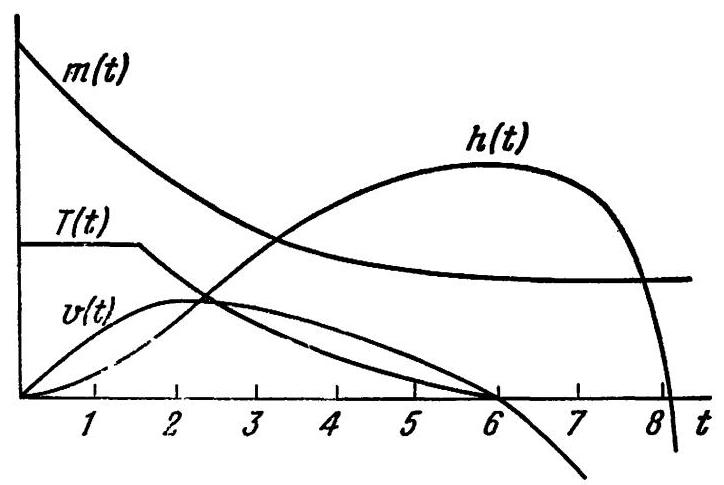
\includegraphics[max width=0.6\textwidth]{images/bo_d547k8bef24c73bgfcg0_498_484_1434_724_485_0.jpg}
\end{center}
\hspace*{3em} 

Рис. 7.14. Кривые высота — скорость в задаче Годдара при лобовом сопротивлении \(D\left( {v,h}\right)  = {v}^{2}{e}^{-h}.\)

для силы лобового сопротивления \({D}_{0}\left( v\right) {e}^{-{\alpha h}},\Gamma\) дel \({D}_{0}\left( v\right)  = {v}^{2}\) и \(\alpha  = 1\) . Обращаем внимание читателя на увеличение максимальной вы- соты, достигнутое путем перехода от программы «полная сила тяги до момента сгорания всего топлива» к программе 4, которая близка к оптимальной программе (см. упражнение 4).

\section*{Упражнения}

1. Показать, что для атмосферы постоянной плотности \(D\left( {v,h}\right)  = {D}_{1}\left( v\right)\) вывод теоремы 13 имеет силу и без требований на \({T}_{1}\) .

2. Вычислить оптимальную программу изменения силы тяги для типовой метеорологической ракеты для случая, когда сила лобового сопротивления резко возрастает с приближением скорости ракеты к скорости звука.

\begin{center}
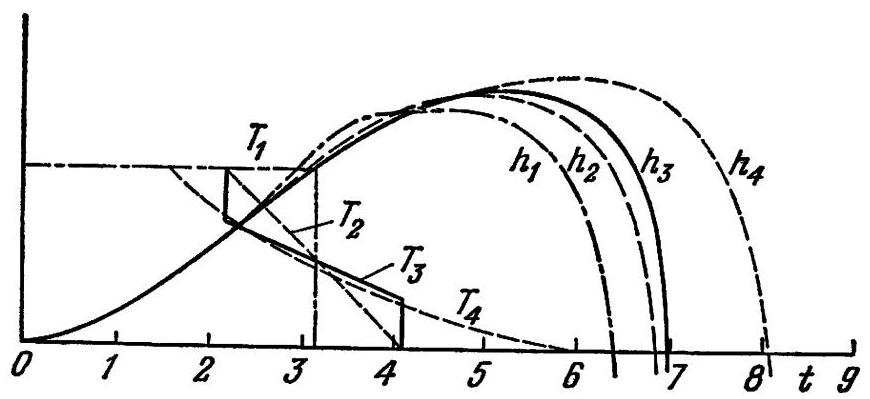
\includegraphics[max width=0.8\textwidth]{images/bo_d547k8bef24c73bgfcg0_499_355_669_870_399_0.jpg}
\end{center}
\hspace*{3em} 

Рис. 7.15. Сравнение высот в задаче Годдара для программ силы тяги 1 — 4.

3. Доказать существование оптимального управления для системы ура в нений \({\mathcal{L}}_{0}\) при условии, что функция \(D\left( {v,h}\right)\) кусочно-дифференпируема и \({vD}\left( {v,h}\right)  \geq  0\) (см. теорему 4 главы 4).

4. Пополнить совокупность программ изменения силы тяги построением оптимального решения в численном примере для задачи Годдара, которая была рассмотрена выше в тексте.

\section*{7.3. Управление угловой скоростью твердого тела}

Рассмотрим твердое тело в инерциальной системе отсчета, сво- бодное от всех внешних неинерциальных сил. Пусть о, ку есть компоненты угловой скорости тела относительно жестко свя- занных с телом осей х, у, z прямоугольной системы координат, проходящей через центр тяжести, и пусть через \({I}_{x},{I}_{y},{I}_{z}\) обо- значены главные моменты инерции (положительные действительные числа). Предположим, что мы можем приложить к телу вращаю- щие моменты при помощи управляемых газовых струй. Обозначим эти моменты через \({u}_{x},{u}_{y}\) и \({u}_{z}\) в зависимости от осей, относительно которых они действуют. Уравнение движения Эйлера для этой задачи имеет такой вид:

\[
{I}_{x}{\dot{\omega }}_{x} = {\omega }_{y}{\omega }_{z}\left( {{I}_{y} - {I}_{z}}\right)  + {b}_{x}{u}_{x},
\]

(Q)
\[
{I}_{y}{\omega }_{y} = {\omega }_{z}{\omega }_{x}\left( {{I}_{z} - {I}_{x}}\right)  + {b}_{y}{u}_{y}
\]

\[
{I}_{z}{\omega }_{z} = {\omega }_{x}{\omega }_{y}\left( {{I}_{x} - {I}_{y}}\right)  + {b}_{z}{u}_{z}
\]

где \({b}_{x},{b}_{y},{b}_{z}\) - положительные константы. Естественно предполо- жить, что сила, с которой управляющие газовые струи действуют на твердое тело, ограничена. Мы рассмотрим два случая.

1) Для каждой оси имеется пара управляемых струй, создаю- щих независимые вращающие моменты для каждой оси, причем \(\left| {u}_{i}\right|  \leq  1,i = x,y,z\) .

2) Имеется в распоряжении только одна пара управляемых струй, но газовые сопла могут быть установлены под любым углом относительно твердого тела. Наложенное на управление ограни- чение принимает вид \(\parallel u{\parallel }^{2} = {u}_{x}^{2} + {u}_{y}^{2} + {u}_{z}^{2} \leq  1\) .

Задачей управления является остановка вращающегося объекта оптимальным способом, в частности, требуется дать синтез управ- ления с обратной связью, который обеспечивал бы оптимальное уиравление для каждой начальной угловой скорости. Оптималь- ность будет выражена в терминах наименьшего затраченного вре- мени, или минимального расхода топлива или энергии в течение заданного интервала времени. В следующем разделе мы рассмот- рим задачу о существовании оптимальных управлений.

\section*{Существование оптимальных управлений}

Рассмотрим упомянутую выше систему уравнений Q с началь- ной угловой скоростью ( \({\omega }_{x0},{\omega }_{y0},{\omega }_{z0}\) ) в момент t=0. Мы сначала покажем, что в каждом случае, 1) или 2), существует допустимое управление, переводящее систему Q с начальными условиями \(\left( {{\omega }_{x0},{\omega }_{y0},{\omega }_{z0}}\right)\) вдоль траектории \(\left( {{\omega }_{x}\left( t\right) ,{\omega }_{y}\left( t\right) ,{\omega }_{z}\left( t\right) }\right)\) в точку \(\left( {0,0,0}\right)\) в течение конечного промежутка времени. Положим \(J = \frac{1}{2}\left( {{I}_{x}{\omega }_{x}^{2} + {I}_{y}{\omega }_{y}^{2} + {I}_{z}{\omega }_{z}^{2}}\right)\) и построим синтез управления с обрат- ной связью:

где

\[
{u}_{x} =  - \frac{1}{2}\frac{\alpha {I}_{x}{\omega }_{x}}{{b}_{x}{J}^{1/2}},\;{u}_{y} =  - \frac{1}{2}\frac{\alpha {I}_{y}{\omega }_{y}}{{b}_{y}{J}^{1/2}},\;{u}_{z} =  - \frac{1}{2}\frac{\alpha {I}_{z}{\omega }_{z}}{{b}_{z}{J}^{1/2}},
\]

\[
\alpha  = \min \left\{  {\frac{{b}_{x}}{{I}_{x}^{1/2}},\;\frac{{b}_{y}}{{I}_{y}^{1/2}},\;\frac{{b}_{z}}{{J}_{z}^{1/2}}}\right\}  .
\]

Очевидно, что \(\left( {{u}_{x}^{2} + {u}_{y}^{2} + {u}_{z}^{2}}\right)  \leq  1\) и \(\left| {u}_{x}\right|  \leq  1,\left| {u}_{y}\right|  \leq  1,\left| {u}_{z}\right|  \leq  1\) . Вычислим dJ/dt вдоль решений системы Q при указанном выше управлении с обратной связью:

\[
\frac{dJ}{dt} = \frac{-\frac{1}{2}\alpha }{{J}^{1/3}}\left\lbrack  {{I}_{x}{\omega }_{x}^{2} + {I}_{y}{\omega }_{y}^{2} + {I}_{z}{\omega }_{z}^{2}}\right\rbrack   =  - \alpha {J}^{1/3}.
\]

\(\Pi\) ycть \(W = {J}^{1/2}\) . Тогда W \(=  - \frac{1}{2}\alpha\) (при ме 0). Таким образом, величина \(W\left( t\right)\) для каждого заданного начального условия приво- дится к нулю за конечное время и то же имеет место для \(J = {W}^{2}\) . Вследствие неотрицательности величины \(J\) соотношение \(J = 0\) озна- чает, что \({\omega }_{x} = {\omega }_{y} = {\omega }_{z} = 0\) . Tenepь надо показать, что каждое решение системы Q при ограничениях 1) или 2) является равно- мерно ограниченным на каждом конечном отрезке времени [0, τ]. Рассмотрим указанную выше функцию J. Для этой функции

\[
\frac{dJ}{dt} = {\omega }_{x}{b}_{x}{u}_{x} + {\omega }_{y}{b}_{y}{u}_{y} + {\omega }_{z}{b}_{z}{u}_{z}.
\]

Oveвидно, что

\[
\left| \frac{dJ}{dt}\right|  \leq  \gamma {J}^{1}/2
\]

при некотором постоянном \(\gamma \left( {0 \leq  \gamma  < \infty }\right)\) , если мы примем во вни- мание ограничение 1), которое содержит в себе ограничение 2) и, следовательно,

\[
0 \leq  J\left( t\right)  \leq  {\left( \gamma t + c\right) }^{2}
\]

для некоторой константы с (0 ≤ c < ∞). Таким образом, каждое решение, начинающееся в точке ( \({\omega }_{x0},{\omega }_{y0},{\omega }_{z0}\) ), является равномер- но ограниченным на каждом конечном интервале времени 0 ≤ t ≤ τ . Ясно, что в рассматриваемом случае для задачи оптимального бы- стродействия выполняются условия выпуклости и непрерывности теоремы существования 4 главы 4. Только что мы как раз пока- зали, что всегда имеется допустимое управление, переводящее каждое начальное состояние в начало координат за конечный от- резок времени и что все решения равномерно ограничены на каждом конечном интервале времени. Это имеет место даже в рас- ширенном фазовом пространстве, когда добавляется координата времени —критерия качества. Таким образом, существование управления, оптимального по быстродействию, установлено при любом из ограничений 1) или 2).

Задача минимальной затраты энергии, которую мы теперь рас- смотрим, есть задача приведения системы Q из начальной точки \(\left( {{\omega }_{x0},{\omega }_{y0},{\omega }_{z0}}\right)\) в точку (0,0,0) за время T, где T — фиксиро- ванное конечное число, при помощи управления, доставляющего минимум критерию качества

\[
{x}_{E}^{0}\left( T\right)  = \frac{1}{2}{\int }_{0}^{T}\parallel u\left( t\right) {\parallel }^{2}{dt}
\]

Задача минимизации топлива 1) аналогична этой задаче, за исключением того, что критерий качества здесь другой, а именно,

\[
{x}_{F}^{0}\left( T\right)  = {\int }_{0}^{T}\parallel u\left( t\right) \parallel {dt}
\]

\HRule

1) Используемые здесь термины «топливо» и «энергия» могут не соответ- ствовать обычным физическим понятиям топлива и энергии.

\HRule

Если добавить координату качества xE (или xF), соответствующую значению критерия качества, к основной системе, то предположе- ние нашей основной теоремы существования 4 главы 4 о выпукло- сти нарушается. Однако обе координаты качества как в случае 1), так и в случае 2), удовлетворяют теореме существования из упраж- нения 2.2 главы 4. Мы уже установили существование равномерно ограниченного основного решения ( \({\omega }_{x}\left( t\right) ,{\omega }_{y}\left( t\right) ,{\omega }_{z}\left( t\right)\) ) на каждом ко- нечном интервале времени, и легко видеть, что координаты ка- чества также являются ограниченными, если учитываются огра. ничения 1) или 2). Таким образом, оптимальные управления топливом и энергией существуют, если основной интервал времени \(\left( {0,T}\right)\) является по крайней мере столь же большим, как и время, требуемое для перехода системы из состояния ( \({\omega }_{x0},{\omega }_{y0},{\omega }_{z0}\) ) в состояние \(\left( {0,0,0}\right)\) в задаче оптимального быстродействия.

Мы далее рассмотрим только задачу оптимального быстродей- ствия для иллюстрации применения изложенной теории. Задачи минимизации расхода топлива и затраты энергии можно тракто- вать аналогичным образом, и мы предпочитаем их решение оста- вить читателю в качестве упражнений. При этом мы обращаем внимание читателя на теорему существования из упражнения 2.2 главы 4.

\section*{Синтез управления, оптимального по быстродействию}

Рассмотрнм приведенную вышесистему уравнений \(Q\) при огра- ничении на управление \({u}_{x}^{2} + {u}_{y}^{2} + {u}_{z}^{2} \leq  1\) ,и предположим,что \({b}_{1} = \; = {b}_{2} = {b}_{3}\) , T. e. что воздействие управляющего фактора на систему одинаково в каждом направлений. Мы теперь непосредственно покажем,что реиенце забачи олмциальноzo быспробейспвия при оуаничении 2) дается следующнм выбором управления собратной CBA3bIO:

\[
{u}_{x}^{ * } =  - \frac{{I}_{x}{\omega }_{x}}{{M}^{1/2}},\;{u}_{y}^{ * } =  - \frac{{I}_{y}{\omega }_{y}}{{M}^{1/2}},\;{u}_{z}^{ * } =  - \frac{{I}_{z}{\omega }_{z}}{{M}^{1/2}},
\]

где

\[
M = {I}_{x}^{2}{\omega }_{x}^{2} + {I}_{y}^{2}{\omega }_{y}^{2} + {I}_{z}^{2}{\omega }_{z}^{2}.
\]

Ouebhдно, что

\[
{u}_{x}^{*2} + {u}_{y}^{*2} + {u}_{z}^{*2} \leq  1
\]

Легко показать, используя неравенство ШВарца, что

\[
- 1 \leq  \frac{d{M}^{1/2}}{dt} \leq  1
\]

вдоль любого пути при упомянутом ограничении 2) на управление.

Более того, если используется управление и*, то

\[
\frac{d{M}^{*1/2}}{dt} =  - 1
\]

и и* переводит систему в начало координат за конечное время, как показывает исследование, аналогичное проведенному в пре- дыдущем разделе. Сравнивая упомянутые выше дифференциальные неравенства, можно вычислить время, соответствующее указанно- му управлению с обратной связью. Таким образом, максималь- ная амплитуда оптимального управления равна единице, а вектор оптимального управления прямо противоположен вектору кинети- ческого момента ( \({I}_{x}{\omega }_{x},{I}_{y}{\omega }_{y},{I}_{z}{\omega }_{z}\) ).

Более общие задачи, называемые задачами с инвариантной нормой, можно исследовать таким же образом, как упомянутую выше задачу оптимального быстродействия при ограничении 2) (см. упражнение 1).

Обратимся теперь к методу построения синтеза управления с обратной связью для задачи оптимального быстродействия при ограничении 1), т. е. когда \(\left| {u}_{x}\right|  \leq  1,\left| {u}_{y}\right|  \leq  1,\left| {u}_{z}\right|  \leq  1\) . Для про- стоты предположим, что твердое тело обладает центральной сим- метрией, а именно, \({I}_{x} = {I}_{y}\) . Для этого случая, когда первые два главных момента инерции равны, уравнения Эйлера принимают вид

\[
\left( {Q}_{s}\right)
\]

\[
\text{ ;) }\;{\dot{\omega }}_{x} = \alpha {\omega }_{y}{\omega }_{z} + {\beta }_{x}{u}_{x},\;{\dot{\omega }}_{y} =  - \alpha {\omega }_{x}{\omega }_{z} + {\beta }_{y}{u}_{y},\;{\dot{\omega }}_{z} = {\beta }_{z}{u}_{z}\text{ , }
\]

rne

\[
\alpha  = \left( {{I}_{y} - {I}_{z}}\right) {I}_{x}\text{ и }{\beta }_{x} = \frac{{b}_{x}}{{I}_{x}},\;{\beta }_{y} = \frac{{b}_{y}}{{I}_{y}},\;{\beta }_{z} = \frac{{b}_{z}}{{I}_{z}}.
\]

Как и в главе 4, определим гамильтониан

\[
H = {\eta }_{1}\left\lbrack  {\alpha {\omega }_{y}{\omega }_{z} + {\beta }_{x}{u}_{x}}\right\rbrack   + {\eta }_{2}\left\lbrack  {-\alpha {\omega }_{x}{\omega }_{z} + {\beta }_{y}{u}_{y}}\right\rbrack   + {\eta }_{3}{\beta }_{z}{u}_{z},
\]

где вектор-функция \(\left( {{\eta }_{1},{\eta }_{2},{\eta }_{3}}\right)\) yдовлетворяет системе дифферен- циальных уравнений

\[
{\dot{\eta }}_{1} =  - \frac{\partial H}{\partial {\omega }_{x}} = \alpha {\omega }_{z}{\eta }_{2},
\]

(A)
\[
{\dot{\eta }}_{2} =  - \frac{\partial H}{\partial {\omega }_{y}} =  - \alpha {\omega }_{z}{\eta }_{1}
\]

\[
{\dot{\eta }}_{3} =  - \frac{\partial H}{\partial {\omega }_{z}} =  - \alpha {\omega }_{y}{\eta }_{1} + \alpha {\omega }_{z}{\eta }_{2}.
\]

Первый интеграл этой системы имеет вид пц тирете ли зак как функции \({\eta }_{1},{\eta }_{2},{\eta }_{3}\) входят в \(H\) линейно, то предположим, что | \({\eta }_{1}\left( 0\right) \left| +\right| {\eta }_{2}\left( 0\right) \left| +\right| {\eta }_{3}\left( 0\right) | = 1\) . Это условие не меняет распо- ложения нулей функций \({\eta }_{i}\left( t\right) ,i = 1,2,3\) .

Принцип максимума устанавливает, что если управление \(\left( {{u}_{x}\left( t\right) ,{u}_{y}\left( t\right) ,{u}_{z}\left( t\right) }\right.\) onтимально, то оно должно максимизировать функцию Н. Поэтому для известных \({\omega }_{i}\left( t\right) ,{\eta }_{i}\left( t\right)\)

\[
{u}_{i}\left( t\right)  = \begin{cases} 1, & \operatorname{ec\text{ л }\text{ и }}{\eta }_{i}\left( t\right)  > 0, \\   - 1, & \operatorname{ec\text{ л }\text{ и }}{\eta }_{i}\left( t\right)  < 0,i = x,y,z,u\text{ ли }1,2,3, \end{cases}
\]

Таким образом, управление и (t) = ( \({u}_{x}\left( t\right) ,{u}_{y}\left( t\right) ,{u}_{z}\left( t\right)\) ) вполне определяется вектором \(\eta \left( t\right)  = \left( {{\eta }_{1}\left( t\right) ,{\eta }_{2}\left( t\right) ,{\eta }_{3}\left( t\right) }\right)\) в любой момент времени, в который все координаты вектора η (t) отличны от нуля. Таким образом, оказывается, что нули функций упа, \({\eta }_{3}\left( t\right)\) urpaют специальную роль в определении максимальных управлений. Если общее время, в течение которого вектор η (t) обращается в нуль, имеет меру нуль, то управления определены почти всюду.

Рассмотрим теперь систему уравнений . Предположим, что \({\eta }_{1}\left( 0\right)  = {\eta }_{2}\left( 0\right)  = 0;\) тогда и в соотношений \({\eta }_{1} = 0,{\eta }_{2} = 0,{\eta }_{3} = 0\) сле- дует,что \({\eta }_{1}\left( t\right)  = 0,{\eta }_{2}\left( t\right)  = 0,{\eta }_{3}\left( t\right)  = 1\) или -1. Эти соотноше- ния определяют лишь управление \({u}_{z}\left( t\right)\) , a этого недостаточно. Тем не менее, и в этом случае есть метод, который можно исполь- зовать для построения оптимальных траекторий, ведущих в на- чало координат. Заменим \(t\) на - \(t\) в системах \({Q}_{s}\) и \(\mathcal{A}\) и выберем в качестве начальных условий точку о \({\omega }_{x}\left( 0\right)  = {\omega }_{y}\left( 0\right)  = {\omega }_{z}\left( 0\right)  = 0\) . При этом вектор \(\left( {{\eta }_{1}\left( 0\right) ,{\eta }_{2}\left( 0\right) ,{\eta }_{3}\left( 0\right) }\right)\) выберем так, tuтобы \(\left| {{\eta }_{1}\left( 0\right) }\right|  + \left| {{\eta }_{2}\left( 0\right) }\right|  + \left| {{\eta }_{3}\left( 0\right) }\right|  = 1\) . Рассмотрим далее решение уравне- ний \({Q}_{s}\) и \(\mathcal{A}\) на интервале τ < t < 0 при максимальном управле- нии. При \(t\) ,изменяющемся от 0 до τ,точка ( \({\omega }_{x}\left( t\right)\) , \({\omega }_{y}\left( t\right)\) , \({\omega }_{z}\left( t\right)\) ) описывает специальное множество точек, называемое максималь- ной траекторией. При всевозможных значениях вектора (η, (1), \(\left. {{\eta }_{2}\left( 0\right) ,{\eta }_{3}\left( 0\right) }\right)\) ,подчиненных условию \(\left| {{\eta }_{1}\left( 0\right) }\right|  + \left| {{\eta }_{2}\left( 0\right) }\right|  + \left| {{\eta }_{3}\left( 0\right) }\right|  = 1\) , получаются все максимальные траектории, проходящие через на- чало координат. Среди этих максимальных траекторий содержатся оптимальные траектории. Поэтому, если имеется лишь конечное число максимальных траекторий, соединяющих заданную точку с началом координат, из них можно выбрать оптимальную траек- торию. Вдоль этой оптимальной траектории управление известно, и может быть выражено как функция переменных ( \({\omega }_{x},{\omega }_{y},{\omega }_{z}\) ); эта функция и является искомым управлением для всех точек, которые лежат на рассматриваемой траектории. Если найдено плотное множество непересекающихся оптимальных траекторий, то Гоптимальное управление известно почти всюду. Это и есть информация, требуемая для вычисления управляющей функции с обратной связью. Этот метод (метод попятного движения) ис- пользован при нахождении управления с обратной связью в разделе 7.1.

Вернемся теперь к определению максимальных управлений, в случаё,когда \({\eta }_{1}\left( t\right)  = 0,{\eta }_{2}\left( t\right)  = 0,{\eta }_{3}\left( t\right)  = 1\) или-1. Пля опре- деленности рассмотрнм случай,когда \({\eta }_{3}\left( t\right)  = 1\) . Взяв качестве начальнойточки точку \({\omega }_{x}\left( 0\right)  = {\omega }_{v}\left( 0\right)  = {\omega }_{z}\left( 0\right)  = 0\) иперебрав все улравления \(u = \left( {{u}_{x},{u}_{v},{u}_{z}}\right)\) внда \({u}_{z}\left( t\right)  = 1\) и \(\left| {{u}_{x}\left( t\right) }\right|  \leq  1\) , \(\left| {{u}_{v}\left( t\right) }\right|  \leq  1\) or \(\mathrm{p}\) nearehene ha httpbare \({t}_{1} \leq  t \leq  0\) ,получим неко- торый конус \(\bar{K}\) , состоящий целиком из соответствующих траекто- рий. Легко показать, что этот конус непрерывно увеличивается при \({t}_{1} \rightarrow  \tau\) . Очевидно, что первое значение те пременной време- ни \({t}_{1}\) ,для которого точка ( \({\omega }_{x}\) , \({\omega }_{y}\) , \({\omega }_{z}\) ) находится в этом конусе, определит наименьший интервал времени для обратной задачи — задачи перевода начальной точки в начало координат. Так как \({u}_{z}\) .(t) должно быть равно +1, то в качестве и ж,(t), \({u}_{v}\) (t) можно взять любые допустимые управления, удовлетворяющие ограниче- ниям \(\left| {{u}_{x}\left( t\right) }\right|  \leq  1,\left| {{u}_{y}\left( t\right) }\right|  \leq  1\) и переводящие точку ( \({\omega }_{x}\) , \({\omega }_{y}\) ) в точку \(\left( {0,0}\right)\) на интервале ( \({t}^{ * },0\) ). Нетрудно показать, что точка \(\left( {{\omega }_{x},{\omega }_{y},{\omega }_{z}}\right)\) лежит внутри некоторого меньшего конуса, который получится, если на некотором интервале [t, 0] использовать управления \({u}_{x}\left( t\right)  = {u}_{y}\left( t\right)  = 0\) , a затем любые допустимые управле- ния на интервале [t*, t’a].

Для плоского случая ( \(\left( {{\omega }_{x},{\omega }_{y}}\right)\) можно показать, что если и \(= {u}_{y}\left( t\right)  = 0\) на интервале \(\left\lbrack  {{t}_{a},0}\right\rbrack\) ,то при \(t \in  \left\lbrack  {{t}^{ * },{t}_{a}}\right\rbrack\) в качестве \({u}_{x}\left( t\right)\) и \({u}_{v}\left( t\right)\) можно взять релейные управления, которые един- ственным образом определяются значением вектора \({\eta }_{1}\left( t\right) ,{\eta }_{2}\left( t\right)\) , если

\[
\left| {{\eta }_{1}\left( {t}_{a}\right) }\right|  + \left| {{\eta }_{2}\left( {t}_{a}\right) }\right|  > 0.
\]

Неединственность выбора оптимального управления в общем слу- чае объясняется, грубо говоря, тем, что в силу самого характера исследуемой трехмерной системы од может оказаться настолько большим в сравнении с о, и мог, что для приведения о, к 0 тре- буется гораздо больше времени. В этом случае задача распадается на две, по существу, независимые: а) приведение @\_k 0; 6) приве- дение \({\omega }_{x}\) и до; к 0; результирующую задачу можно решить, ре- шая задачи а) и б) последовательно; при этом некоторая неопти- мальность полученного на первом этапе управления может быть скомпенсирована соответствующим выбором управления на вто- ром этапе.

Посмотрим, при каких еще значениях координат \({\eta }_{i}\) соответст- вующее управление определяется неединственным образом. Пред- положим, что функция \({\eta }_{1}\left( t\right)\) на некотором интервале обращается в нуль; следовательно \({\eta }_{1}\left( t\right)  \equiv  0 \equiv  \alpha {\omega }_{z}{\eta }_{2}\) . Тогда или ди,(t) ≡0, или \({\omega }_{z} \equiv  0\) . Если \({\omega }_{z} \equiv  0\) . To \({\omega }_{z} \equiv  0 = {\beta }_{z}{u}_{z}\) и, cледовательно, \({\eta }_{3} \equiv  0\) . Но тогда \({\eta }_{3} \equiv  0\) ,т. e. \({\eta }_{1}{\omega }_{y} = {\omega }_{x}{\eta }_{2}\) и \({\eta }_{1}{\beta }_{x}\operatorname{sgn}{\eta }_{2} \equiv  {\eta }_{2}{\beta }_{y}\operatorname{sgn}{\eta }_{1}\) , что, как легко показать, невозможно. Если ну, не не не не не не \(u\) , \(\operatorname{C\text{ л }\text{ е }\text{ д }\text{ о }\text{ в }\text{ а }\text{ т }\text{ е }\text{ л }\text{ ь }\text{ н }\text{ о },}{\eta }_{3}\left( t\right)  \equiv  0\) ,и так как \(\left| {\eta }_{3}\right|  = 1\) , to мы пришли к случаю, рассмотренному ранее. Предположим, наконец, что \({\eta }_{3}\left( t\right)  \equiv  0\) ; тогда \({\eta }_{3}\left( t\right)  \equiv  0\) и \({\eta }_{1}{\omega }_{v} = {\omega }_{x}{\eta }_{2}\) ,что невозможно. Таким образом, вектор \(\left\lbrack  {{\eta }_{1}\left( t\right) ,{\eta }_{2}\left( t\right) ,{\eta }_{3}\left( t\right) }\right\rbrack\) onpeдeляет управление не единственным образом, лишь когда и, и слу а мое мое мое мое мое мета нусе, описанном ранее. Поэтому в качестве оптимального управ- ления \({u}_{x}\) н \({u}_{y}\) может быть выбрано релейное управление,авыше было показано, как оптимальное управление можно определить экспериментально.

Мы не будем далее продолжать этот анализ. Выше было ука- зано, как можно найти оптимальные траектории, и если эта ин- формация получена, она может храниться при помощи, например, логической схемы (см. [Смит], где описана соответствующая про- цедура). Остается еще вопрос, не проходят ли две максимальные (или оптимальные) траектории через одну и ту же точку. Ниже в упражнениях приводится пример системы, для которой имеются начальные точки, через которые проходят две оптимальные траек- тории.

\section*{Упражнения}

1. Рассмотрим систему нелинейных дифференциальных уравнений (в век- торном обозначении)

(F)
\[
\dot{x} = f\left( {x,t}\right)  + u\left( t\right)  \cdot  \mathrm{B}{R}^{n},
\]

с ограничивающим множеством \(\Omega  \subset  {R}^{m}\)

\[
\Omega  : \parallel u\parallel  \leq  k\text{ для некоторого }k > 0\text{ . }
\]

3десь

\[
\parallel u{\parallel }^{2} = \mathop{\sum }\limits_{{i = 1}}^{m}{\left( {u}^{i}\right) }^{2}
\]

Предположим, что указанная выше система 8 обладает тем свойством, что все решения однородного уравнения

\[
\dot{x} = f\left( {x,t}\right)
\]

лежат на сфере в \({R}^{n}\) ,т. е.

\[
\parallel x\left( t\right) \parallel  = \parallel x\left( 0\right) \parallel \text{ для всех }t \geq  0.
\]

Требуется рассмотреть задачу наискорейшего попадания в начало координат и показать, что оптимальное по быстродействию управление с обратной связью имеет вид

\[
{u}^{ * }\left( t\right)  = \frac{-{kx}\left( t\right) }{\parallel x\left( t\right) \parallel }
\]

где \(x\left( t\right)\) есть текущее состояние системы.

2. Рассмотрим систему Q уравнений движения Эйлера для твердого тела в свободном пространстве. Предположим, что I, \(x \neq  {I}_{y} \neq  {I}_{z}\) и что угло- вая скорость \({\omega }_{x}\left( t\right)\) может быть измерена на интервале [0, \({t}_{1}\) ], \(\left( {{t}_{1} > 0}\right)\) rupo- скопическим прибором.

(a) Показать, что если \({u}_{i}\left( t\right)  \equiv  0,i = x,y,z\) на интервале [0, \({t}_{1}\) ], то не- возможно вычислить \({\omega }_{v}\left( 0\right) ,{\omega }_{z}\left( 0\right)\) ,зная \({\omega }_{x}\left( t\right)\) на интервале [0, \({t}_{1}\) ].

(b) Показать, что если на интервале [0, t] и/q=0, а на интервале \(\left\lbrack  {{t}_{1},{t}_{2}}\right\rbrack  {u}_{i}\left( t\right)  = {k}_{i}\) ,где \({k}_{i} \neq  0,\left( {0 < {t}_{1} < {t}_{2},i = x,y,z}\right)\) , To можно определить оба числа о, (0) и мо¿ (0), если известна система Q и (и(t), ох (t)) на интер- вале 0< t < t > .

\section*{7.4. Оптимальная астронавигация}

Мы рассмотрим задачу управления на расстоянии ракетным кораблем в межпланетном пространстве при минимальной затрате топлива. В типичной задаче такого типа требуется привести корабль из начального фазового состояния (положение, скорость) в Солнечной системе в некоторое предписанное фазовое состояние (цель). Это—общая задача встречи при (или без) предписанной продолжительности полета. Такая общая задача пока не решена сколько-нибудь эффективным способом, и мы упростим эту задачу так, что элементарное, но важное решение можно будет вычислить.

Мы будем искать управление, переводящее корабль с одной эллиптической орбиты Кеплера на другую при минимальном удель- ном импульсе. Никакого ограничения на место или время встречи не накладывается. Будем рассматривать лишь орбиты, располо- женные в одной фиксированной плоскости, содержащей Солнце в начале координат (x, y). Мы рассмотрим эллипсы, один фокус которых фиксирован (совпадает с Солнцем), а другой фокус лежит на заданной линии —оси х. Таким образом, каждый такой эллипс полностью определяется двумя действительными параметрами f и l (движение по всем эллиптическим траекториям происходит так, что радиус-векторы движущейся точки вращаются в одну и ту же сторону), где f-абсцисса второго фокуса (— ∞ < f-<∞) \(l\) -длина большой оси \(\left( {l > 0}\right)\) . Обычные параметры эллипса

\[
c = \frac{\left| f\right| }{2},\;a = \frac{l}{2},\;e = \frac{c}{a}.
\]

Kpyroвые орбиты соответствуют значению \(f = 0\) (эксцентриситет \(e = 0)\) и имеют диаметры, paвные \(l\) .

Мы будем считать допустимыми только импульсные силы тя- ги, которые направлены по касательной вдоль эллиптической орбиты точно в моменты прохождения через перигелий или афе- лий. Каждое такое импульсное управление изменяет эллиптиче- скую орбиту заданного типа на новую эллиптическую орбиту рассмотренного типа. Таким образом, допустимое управление со- стоит из конечной последовательности импульсов силы тяги, ка- сательных к орбите в чередующихся точках пересечения положи- тельной и отрицательной полуосей х.

Критерием качества каждого допустимого управления будем считать сумму всех удельных импульсов, т. е. сумму модулей всех изменений скорости.

Представим каждую орбиту Кеплера с заданными параметрами в виде точки на верхней полуплоскости с декартовыми координа- тами f, l >0. Тогда каждое управление можно представить в виде конечной последовательности точек в этой п тоскости, или в виде ломаной, соединяющей начальную и конечную орбиты.

Если орбита имеет координаты f >0, l >0, то сила тяги (направленная назад или вперед) в афелии (в момент перехода при \(x > 0\) ) coxpaняer афелиальное расстояние (l+f)/2. Анало- гичная проверка всех возможных случаев приводит к заключению, что силы тяги при \(x > 0\) не меняют величины (l+f)/2, a силы тяги при \(x < 0\) не меняют величину (l—f)/2. Поэтому ломаная, изображающая любое допустимое управление, должна состоять из чередующихся сегментов с тангенсом угла наклона —l и +1 в плоскости (f, l).

Перейдем теперь к вычислению критерия качества для каждой такой ломаной, характеризующей управление. Как следует из за- конов небесной механики, орбиты Кеплера описываются решениями уравнений Ньютона

\[
\ddot{x} = \frac{-{kx}}{{r}^{3}},\ddot{y} = \frac{-{ky}}{{r}^{3}},
\]

где k есть гравитационная постоянная. Уравнение орбиты в по- лярных координатах (r, θ), как известно, имеет вид

\[
r = \frac{{h}^{2}/k}{1 + e\cos \theta },
\]

где `

\[
{h}^{2} = {ka}\left( {1 - {e}^{2}}\right) ,\;\mathrm{a}\;{r}^{2}\dot{\theta } = h.
\]

Cкорость в перигелии ( \({v}_{\text{ per }}\) ) удовлетворяет уравнению \(\frac{{h}^{2}/k}{1 + e}{v}_{\text{ per }} = h\) , откуда

\[
{v}_{\text{ per }} = \sqrt{\frac{2k}{l}}\sqrt{\frac{l + \left| f\right| }{l - \left| f\right| }}.
\]

llanee,

\[
{v}_{\mathrm{{aph}}} = \sqrt{\frac{2k}{l}}\sqrt{\frac{l - \left| f\right| }{l + \left| f\right| }},
\]

где варь —скорость в афелии. Рассмотрим силу тяги при \(x > 0\) . Если f>0, то это соответствует афелию и удельный импульс есть

\[
{\Delta v} = \Delta \sqrt{\frac{2k}{l}}\sqrt{\frac{l - f}{l + f}}.
\]

В перигелии \(\left( {f < 0}\right)\) удельный импульс вычисляется по формуле

\[
{\Delta v} = \Delta \sqrt{\frac{2k}{l}}\sqrt{\frac{l - f}{l + f}}.
\]

Тем самым удельный импульс вычисляется в обоих случаях по одной и той же формуле. Поэтому сила тяги в точках, где х > 0, соответствует отрезку ломаной с угловым коэффициентом —1 и критерию качества, равному модулю прирашения величины \(\sqrt{{2k}/l}\sqrt{\left( {l - f}\right) /\left( {l + f}\right) }\) на этом отрезке. Аналогично силе тяги в точ- ках, где \(x < 0\) , cootветствует отрезок ломаной с угловым коэф- фициентом +1 и критерий качества, равный модулю приращения величины \(\sqrt{{2k}/l}\sqrt{\left( {l + f}\right) /\left( {l - f}\right) }\) на указанном отрезке.

В качестве примера применения нашей теории рассмотрим переход с одной из двух заданных эллиптических орбит ( другую \(\left( {{f}_{1},{l}_{1}}\right)\) под действием двух импульсов. Это управление изображается ломаной, состоящей из двух отрезков. Имеются два варианта такого управления (см. рис. 7.16, на котором (f, l) координаты повернуты на \({45}^{ \circ  }\) ). B случае, когда \({f}_{0} = {f}_{1} = 0\) ,т. e. когда начальная и конечные орбиты — круговые, обоим вари- антам соответствует одно и то же значение критерия качества (в силу симметрии) и такое управление называется преобразова- нием орбит Гомана (Hohmann). Мы вычислим критерий качества для преобразования орбит Гомана между круговыми орбитами диаметров \({l}_{0}\) и \({l}_{1} > {l}_{0}\) . Единственная промежуточная орбита Гомана есть эллипс с f=(l,\_-/u)/2 и l = (l, i-/l)/2, который касается на- чальной и конечной окружностей.

\begin{center}
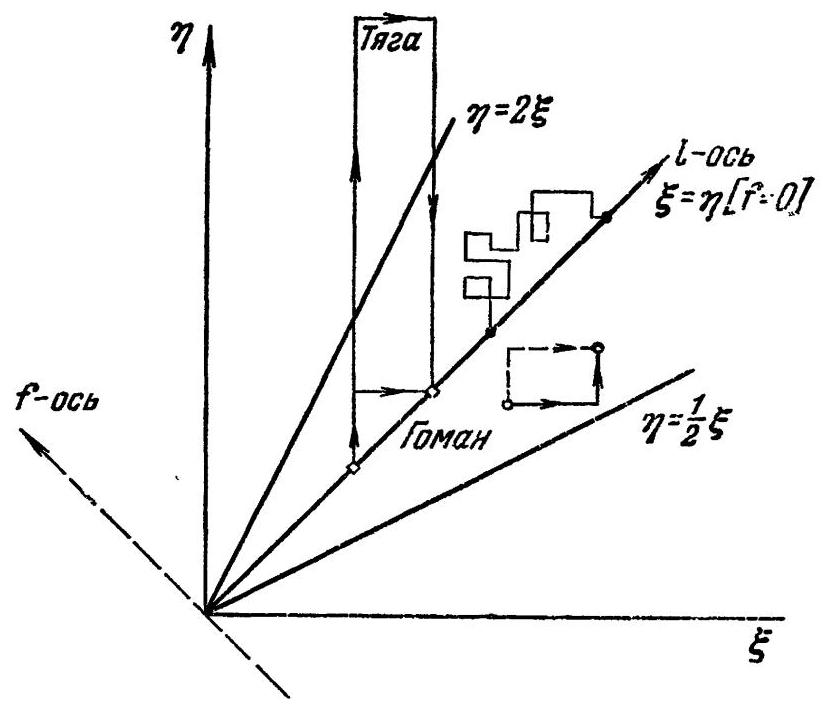
\includegraphics[max width=0.7\textwidth]{images/bo_d547k8bef24c73bgfcg0_509_347_525_823_705_0.jpg}
\end{center}
\hspace*{3em} 

Рис. 7.16. Импульсное управление для перехода с одной эллиптической орбиты на другую.

Первому отрезку (для \(x < 0\) ) соответствует критерий качества

\[
{\Delta v} = \sqrt{\frac{4k}{{l}_{0} + {l}_{1}}}\sqrt{\frac{{l}_{1}}{{l}_{0}}} - \sqrt{\frac{2k}{{l}_{0}}} \cdot  1,
\]

a второму (для \(x > 0\) )-критерий качества

\[
{\Delta v} = \sqrt{\frac{2k}{{l}_{1}}} \cdot  1 - \sqrt{\frac{4k}{{l}_{0} + {l}_{1}}}\sqrt{\frac{{l}_{0}}{{l}_{1}}}.
\]

Если отношение диаметров \({l}_{1}/{l}_{0} = \rho  > 1\) , a масштаб времени выбран так, чтобы начальная орбитальная скорость была единицей

\[
{v}_{0}^{2} = \frac{2k}{{l}_{0}} = 1
\]

то суммарное значение критерия качества равно

\[
C\left( \rho \right)  = \sqrt{\frac{2\rho }{1 + \rho }} - 1 + \sqrt{\frac{1}{\rho }} - \sqrt{\frac{2}{\rho \left( {\rho  + 1}\right) }}.
\]

Конечно, \(C\left( 1\right)  = 0\) ,и мы легко находим,что \(C\left( \frac{3}{2}\right)  = 0,{18},C\left( 2\right)  =\) =0,29. Орбитальное изменение 1<0<2 имеет относительную важность в теории преобразования орбит Гомана, так как ниже мы покажем, что если 1 < ρ < 2, то преобразование орбит Гома- на является оптимальным управлением перехода между двумя круговыми орбитами. Заметим для дальнейшего, что производная критерия качества равна

\[
\frac{dC}{d\rho } = \sqrt{\frac{1}{2\rho }}\frac{1}{{\left( 1 + \rho \right) }^{3/2}} - \frac{1}{{2\rho }\sqrt{\rho }} + \frac{\left( 2\rho  + 1\right) }{\sqrt{2}{\left\lbrack  \rho \left( \rho  + 1\right) \right\rbrack  }^{3/2}},
\]

и при 1 < ρ < 2 величина суммы первого и последнего членов превышает величину второго члена, так что \(\frac{dC}{d\rho } > 0\) .

Для \(\rho  = {12}\) имеем \(C\left( {12}\right)  = 0,{534}\) . Сравним это значение со значением критерия качества для управления, составленного из трех импульсов силы тяги: сначала очень большой силой тяги при \(x < 0\) ,затем малой тягой при \(x > 0\) и,наконец,большой тягой при \(x < 0\) . Вначале это управление переводит ракетный корабль с первой круговой орбиты на очень вытянутый эллипс, затем на эллипс, незначительно измененный по сравнению с предыдущим и касающийся последней круговой орбиты. На третьем этапе корабль замедляется и переходит на последнюю круговую орбиту. Маневр этого типа можно выбрать, чтобы дать сколь угодно хорошую аппроксимацию параболическому выходу с первой окруж- ности, оценить поведение критерия качества на бесконечности и аппроксимировать параболическое возвращение на желаемую кру- говую орбиту. Учитывая, что скорость параболического перехода всегда в \(\sqrt{2}\) раз больше круговой орбитальной скорости, мы можем вычислить значение критерия качества для этого управления, состоящего из трех импульсов силы тяги:

\[
{C}_{\infty }\left( {12}\right)  = \left\lbrack  {\sqrt{2} - 1}\right\rbrack   + 0 + \left\lbrack  {\sqrt{2}\sqrt{\frac{1}{12}} - \sqrt{\frac{1}{12}}}\right\rbrack   = 0,{533}.
\]

Для произвольного значения ρ>1 этот переход, состоящий из трех импульсов силы тяги, дает вблизи бесконечности следующее значение для критерия качества: \({C}_{\infty }\left( \rho \right)  = 0,{414}\left\lbrack  {1 + \sqrt{\rho }/\rho }\right\rbrack\) . Поэтому мы заключаем, что при ρ≥12 преобразование Гомана уже не является оптимальным управлением в классе допустимых импульс- ных управлений. Итак наша теория показывает, что круговой орбитальный переход из окрестности Земли в окрестность Венеры или Марса можно осуществить наиболее эффективно с помощью преобразования Гомана. Однако для перехода из окрестности Земли в окрестность Урана переход Гомана не оптимален.

Мы теперь должны показать, что для малых отношений ρ > 1 переход Гомана является оптимальным. Нам будет удобно чертить графики в координатах (ξ, η), где

\[
\xi  = l - f,\;\eta  = l + f.
\]

B координатах (ξ,η) линия \(f = 0\) переходит в прямую η=ξ. Допустимые управления изображаются ломаными с горизонталь- ными и вертикальными звеньями и с критериями качества, вы- числяемыми в соответствии с изменением функций

\[
\sqrt{\frac{4k\xi }{\left( {\xi  + \eta }\right) \eta }}\text{ It }\sqrt{\frac{4k\eta }{\left( {\xi  + \eta }\right) \xi }}\text{ . }
\]

Таким образом, мы можем найти критерий качества, вычисляя криволинейный интеграл

\[
\int \sqrt{\frac{k\eta }{{\left( \xi  + \eta \right) }^{3}\xi }}{d\xi } + \sqrt{\frac{k\xi }{{\left( \xi  + \eta \right) }^{3}\eta }}{d\eta }.
\]

Рассмотрим совокупность всех допустимых траекторий, соеди- няющих точки \({\xi }_{0} = {\eta }_{0} = {l}_{0}\) и \({\xi }_{1} = {\eta }_{1} = {l}_{1} = \rho {l}_{0}\) , kaждая из которых лежит в секторе

\[
0 < \frac{1}{2}\xi  \leq  \eta  \leq  {2\xi }.
\]

Любую такую траекторию можно заменить ломаной ξ≤η ≤2ξ без изменения критерия качества. Это следует из симметрии функ- ционала, с помощью которого определен критерий качества, отно- сительно линии η = ξ. Далее, любую ломаную можно «улучшить» (уменьшить критерий качества), избавляясь от перемещений вниз при переходе из точки ( \({\xi }_{0},{\eta }_{0}\) ) в точку ( \({\xi }_{1},{\eta }_{1}\) ). Это следует из монотонности критерия качества

\[
\frac{\partial }{\partial \eta }\sqrt{\frac{\eta }{{\left( \xi  + \eta \right) }^{3}\xi }} = {\left\lbrack  \frac{\eta }{{\left( \xi  + \eta \right) }^{3}\xi }\right\rbrack  }^{-1/2}\frac{\xi  - {2\eta }}{{2\xi }{\left( \xi  + \eta \right) }^{4}} < 0.
\]

Любой подъем ломаной над уровнем п, может быть устранен. Это следует из непосредственного вычисления, показывающего, что основанию любого прямоугольника соответствует значение критерия качества меньшее, чем сумме остальных трех сторон. Аналогично, можно избавиться от горизонтального движения влево, подкоррек- тировав управляющую ломаную. Тем самым, каждую ломаную можно улучшить, заменив ее ступенчатой ломаной, всегда подни- мающейся вправо. Покажем, наконец, что каждую ступень ломаной можно выбрать так, чтобы соответствующее значение критерия качества было наименьшим. Мы вычислим значение критерия качества вдоль пути, составленного из левой вертикальной стороны и верхней стороны прямоугольника, и покажем, что оно меньше соответствующего значения вдоль пути, состоящего из нижней стороны и правой вертикальной его стороны. Чтобы это сделать, Mbl проверим, что

\[
\oint \sqrt{\frac{k\eta }{{\left( \xi  + \eta \right) }^{3}\xi }}{d\xi } + \sqrt{\frac{k\xi }{{\left( \xi  + \eta \right) }^{3}\eta }}{d\eta } > 0,
\]

где интеграл взят вдоль контура, обходимого против часовой стрелки и лежащего внутри некоторого углового сектора. По тео- реме Грина, этот криволинейный интеграл равен двойному интегралу по прямугольнику

\[
\iint \left\lbrack  {\frac{\partial }{\partial \xi }\sqrt{\frac{k\xi }{{\left( \xi  + \eta \right) }^{3}\eta }} - \frac{{\partial }_{\varepsilon }}{\partial \eta }\sqrt{\frac{k\eta }{{\left( \xi  + \eta \right) }^{3}\xi }}}\right\rbrack  {d\xi d\eta }.
\]

Подынтегральное выражение имеет тот же самый знак, что и мно- гочлен

\[
q\left( \lambda \right)  = {\lambda }^{3} - 2{\lambda }^{2} + {2\lambda } - 1 = \left( {\lambda  - 1}\right) \left( {{\lambda }^{2} - \lambda  + 1}\right) ,
\]

где \(\lambda  = \eta  \mid  \xi\) лежит в интервале 1 < \(\lambda  < 2\) . Элементарное исследо- вание показывает, что \(q\left( \lambda \right)  > 0\) и, \(c\) ледовательно, \(\kappa\) аждую ступень нашего управления можно выбрать так, чтобы ей соответствовало вогнутое звено ломаной с наименьшим значением критерия качества. Поэтому оптимальное управление внутри сектора — совпадает с преобразованием Гомана, которому соответствует ломаная из двух звеньев: вертикального звена, соедин яющего точку (ξ0, η0) с точкой (ξ0, η1), и горизонтального звена, соединяю- щего точку (ξ0, η1) с точкой (ξ0, η1). Ясно, что при \(1 \leq  \rho  \leq  2\) преобразованию Гомана соответствует ломаная, лежащая в задан- ном секторе.

В заключение мы хотим показать, что на управлениях, которым соответствуют ломаные, лежащие вне этого сектора, критерий качества всегда принимает большее значение, чем на преобразо- вании Гомана, если р > 1 соответствующим образом ограничено. Рассмотрим любую ломаную, соответствующую допустимому управ- лению, ведущему из \({\xi }_{0} = {\eta }_{0} = {l}_{0}\) к границе сектора. Пользуясь описанными выше приемами уменьшения значения критерия ка- чества, можно показать, что оптимальный путь является либо горизонтальным отрезком, либо вертикальным отрезком, либо ломаной, состоящей из вертикального отрезка, за которым следует горизонтальный отрезок. Мы покажем, что для произвольной точки \(\left( {\overline{\xi },\overline{\eta }}\right)\) cextopa \(\xi  \leq  \eta  \leq  {2\xi }\) пути,ведущему из ( \(\overline{\xi },\overline{\eta }\) ) вдоль верти- кальной прямой до пересечения с линией η = 2ξ, соответствует не большее значение критерия качества, чем аналогичному пути вдоль горизонтального отрезка. Это наблюдение, вместе с заме- чаниями, сделанными раньше, позволяет показать, что оптималь- ным путем от точки \({\xi }_{0} = {\eta }_{0} = {l}_{0}\) до линии η \(= {2\xi }\) является верти- кальный отрезок. Для этого надо доказать неравенство

\[
\left| {\sqrt{\frac{4k}{\overline{\xi } + \overline{\eta }}}\sqrt{\frac{\overline{\eta }}{\overline{\xi }}} - \sqrt{\frac{4k}{\overline{\xi } + 2\overline{\xi }}}\sqrt{2}}\right|  \leq
\]

\[
\leq  \left| {\sqrt{\frac{4k}{\overline{\xi } + \overline{\eta }}}\sqrt{\frac{\overline{\xi }}{\overline{\eta }}} - \sqrt{\frac{4k}{3\overline{\eta }/2}}\frac{1}{\sqrt{2}}}\right|
\]

при \(\overline{\xi } \leq  \overline{\eta } \leq  2\overline{\xi }\) . Подстановкой \(\lambda  = \overline{\eta }/\overline{\xi }\) это неравенство приво- дится к виду

\[
\sqrt{\frac{2}{3}} - \sqrt{\frac{\lambda }{1 + \lambda }} \leq  \sqrt{\frac{1}{\lambda \left( {1 + \lambda }\right) }} - \sqrt{\frac{1}{3\lambda }}.
\]

умножая на У \(\overline{\lambda }\) ,получаем эквивалентное неравенство

\[
\frac{\sqrt{2\lambda } + 1}{\sqrt{3}} \leq  \frac{1 + \lambda }{\sqrt{1 + \lambda }} = \sqrt{1 + \lambda }.
\]

Возводя в квадрат и упрощая, получаем

\[
2\sqrt{2\lambda } \leq  2 + \lambda
\]

ИЛИ

\[
{\left( \sqrt{\lambda } - \sqrt{2}\right) }^{2} \geq  0\text{ . }
\]

Поэтому значение критерия качества для вертикального отрезка, ведущего к прямой η = 2ξ, не больше соответствующего значения для горизонтального отрезка, ведущего к той же прямой.

Теперь легко вычислить минимальное значение критерия ка- чества для управления, которое выводит точку ξ0=η0=l0 на границу основного сектора, и затем переводит ее в точку ξ, = η, = \(= {l}_{1} = \rho {l}_{0}\) . Это суммарное значение должно превосходить (если положить \({2k}/{l}_{0} = 1\) ) величину

\[
{C}_{B}\left( \rho \right)  = \left( {\sqrt{\frac{1}{\rho }} + 1}\right) \left( {\sqrt{\frac{4}{3}} - 1}\right) .
\]

Заметим, что \({C}_{B}\left( 2\right)  \geq  0,{26}\mathrm{\text{ и }}{C}_{B}\left( \rho \right)\) есть убывающая функция от \(\rho\) . Мы показали, что

\[
C\left( \rho \right)  < {C}_{B}\left( \rho \right) \text{ при }1 \leq  \rho  \leq  1,8\text{ . }
\]

17 9. B. Ли, Л. Маркув

Это неравенство есть наш главный результат. Оно означает, что преобразование Гомана является оптимальным управлением в классе импульсных управлений между двумя круговыми орбитами

\begin{center}
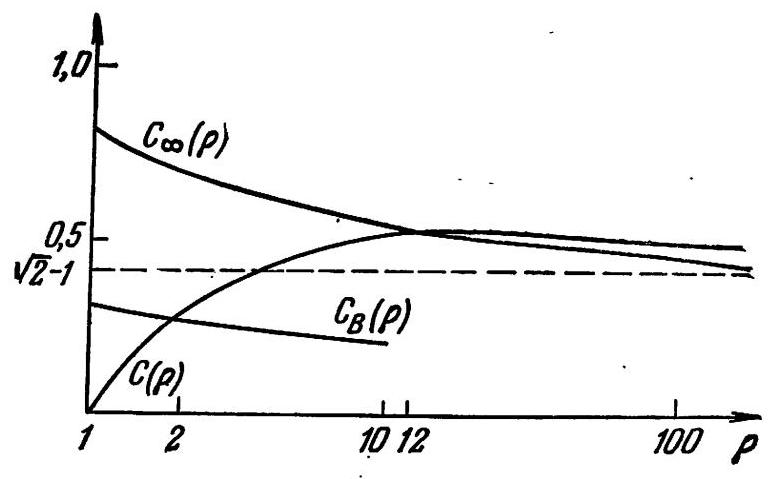
\includegraphics[max width=0.6\textwidth]{images/bo_d547k8bef24c73bgfcg0_514_457_346_774_479_0.jpg}
\end{center}
\hspace*{3em} 

Рис. 7.17. Сравнение критернев качества.

\[
{C}_{\infty }\left( \rho \right)  = \left( {\sqrt{2} - 1}\right) \left( {1 + {\rho }^{-1/2}}\right) .
\]

с отношением диаметров, меньшим, чем ρ = 1,8, даже по сравнению с управлениями, которые значительно изменяются по величине. Весьма вероятно, что переход Гомана оптимален для \(\rho  = 2\) и даже для некоторых значений ρ>2. Однако, как мы показали, пре- образование Гомана уже не оптимально, если ре 212.

Поведение критерия качества в зависимости от ρ иллюстри- руется диаграммой 7.17.

приложение А

\section*{MEТОД НАИСКОРЕЙШЕГО СПУСКА и другие численные методы в зддАЧАХ ОПТИМАЛЬНОГО УПРАВЛЕНИЯ}

Во многих задачах оптимального управления, рассмотренных в предыдущих главах, удавалось получить необходимые и достаточ- ные условия оптимальности. Как правило, в этих случаях мы по- казывали, что основное необходимое условие—принцип макси- мума — является также и достаточным. Для целого ряда задач удалось также разрешить вопросы существования и единственности оптимальных решений. Однако даже в этих случаях задачу не всегда удавалось довести до конца, т. е. выразить оптимальное управле- ние как функцию измеряемых величин начальных и конечных условий. В таких случаях остается нерешенной двухточечная краевая задача —задача нахождения решения системы 2n диффе- ренциальных уравнений, с m начальными условиями и 2n-m конечными условиями.

Такую двухточечную краевую задачу удается иногда решить методом наискорейшего спуска, как в случае, когда для нахождения оптимального управления используется принцип максимума, так и в случае, когда строится последовательность управляющих функ- ций, имеющих пределом оптимальное управление. Этот последний подход, именуемый прямым методом, может быть иногда использо- ван для описания необходимых условий оптимальности по извест- ным свойствам предельного управления; кроме того, если предель- ное управление существует, то бывает возможно доказать сущест- вование оптимального управления. Ниже мы рассмотрим примеры, иллюстрирующие такой конструктивный подход. Основной довод в пользу применения метода наискорейшего спуска или других кон- структивных методов состоит в том, что эти методы позволяют ис- пользовать для построения последовательности приближенных уп- равляющих функций, или получения параметров, определяющих оптимальные управляющие функции, вычислительные машины. Тем самым, после конечного числа итераций может быть получена доста- точно близкая к оптимальной управляющая функция (см. дис- куссию об управлениях с обратной связью в начале главы 7).

В настоящем приложении мы рассмотрим метод наискорейшего спуска для общей задачи оптимизации, и покажем, как он при- меняется для выбора оптимальных управлений. В первом разде- ле дается определение и описание метода для наиболее общей задачи оптимизации. Второй раздел содержит примеры применения метода наискорейшего спуска к задачам оптимального управления. В заключительном разделе рассматривается литература по итера- ционным (численным) методам и соответствующая библиография.

\section*{A1. Метод наискорейшего спуска}

Мы рассмотрим сначала метод наискорейшего спуска в конечно- мерном евклидовом пространстве В". Полученные результаты бу- дут справедливы и для любого другого пространства конечной раз- мерности, со скалярным произведением <. · >, полного в метрике \(\left| \cdot \right|  = \langle  \cdot  , \cdot  {\rangle }^{\frac{1}{2}}\) . Метод наискорейшего спуска может быть применен и в бесконечномерном пространстве, удовлетворяющем тем же усло- виям, например, в гильбертовом пространстве Ж. Норма в про- странстве \({E}^{m}\mathrm{c}\) элементами и \(u = \left( {{u}_{1},\ldots ,{u}_{m}}\right)\) обозначается через

\[
\parallel u\parallel  = {\left( \sum {\left( {u}_{i}\right) }^{2}\right) }^{1/2}
\]

а скалярное произведение элементов-и и v в \({E}^{m}\) как

\[
\langle u,v\rangle  = \mathop{\sum }\limits_{{i = 1}}^{m}{u}_{i}{v}_{i}
\]

Пусть \(C\left( u\right)\) —действительная функция, непрерывно дифферен- цируемая на некотором открытом подмножестве Ф в Е". Для простоты рассмотрим случай \(m = 2\) . Пусть функция \(C = C\left( {{u}_{1},{u}_{2}}\right)\) имеет вид, изображенный на рис. А.1, а точка и" (и и я шарты те м ва,что градиент \(\frac{\partial {C}_{0}}{\partial u} \equiv  \frac{\partial C}{\partial u}\left( {u}^{0}\right)  = {\left\lbrack  \frac{\partial C}{\partial {u}_{1}}\left( {u}^{0}\right) ,\frac{\partial C}{\partial {u}_{2}}\left( {u}^{0}\right) \right\rbrack  }^{\prime }\) не равен нулю. Здесь, как и раньше, штрих означает транспонирование вектора или матрицы. Направлением наискорейшего спуска в точке и" из \({E}^{m}\) называется направление, соответствующее вектору в \({R}^{m}\) с на- чалом в и", вдоль которого скорость изменения функции С по от- ношению к длине дуги является минимальной. Пусть S-множе- ство всех гладких кривых в Е2, проходящих через точку и". Пусть \(\gamma  : {u}_{1} = {u}_{1}\left( s\right) ,{u}_{2} = {u}_{2}\left( s\right)\) есть кривая из \(S\) ,заданная в параметри- ческой форме, где s—длина дуги, измеренная от точки и". По- скольку γ—гладкая кривая, то

\[
{\left( \frac{d{u}_{1}\left( s\right) }{ds}\right) }^{2} + {\left( \frac{d{u}_{2}\left( s\right) }{ds}\right) }^{2} = 1
\]

для всех s. Обозначим направляющие косинусы кривой γ в точке \({u}^{0}\) Через \(\frac{d{u}_{1}}{ds},\frac{d{u}_{2}}{ds}.\)

Для непрерывно дифференцируемой функции \(C\left( u\right)\) скорость изменения \(\mathcal{C}\) по отношениюк длине дуги равна

\[
\frac{dC}{ds} = \frac{\partial {C}_{0}}{\partial {u}_{1}}\frac{d{u}_{1}}{ds} + \frac{\partial {C}_{0}}{\partial {u}_{2}}\frac{d{u}_{2}}{ds}
\]

для любой \(\gamma  \in  S\) . Таким образом, направление наискорейшего спуска из \({u}^{0}\) мы получим,найдя направ- ляющие косинусы du,/ds, du,2/ds, минимизирующие величину \({dC}/{ds}\) при ограничении

\[
{\left( \frac{d{u}_{1}}{ds}\right) }^{2} + {\left( \frac{d{u}_{2}}{ds}\right) }^{2} = 1
\]

\begin{center}
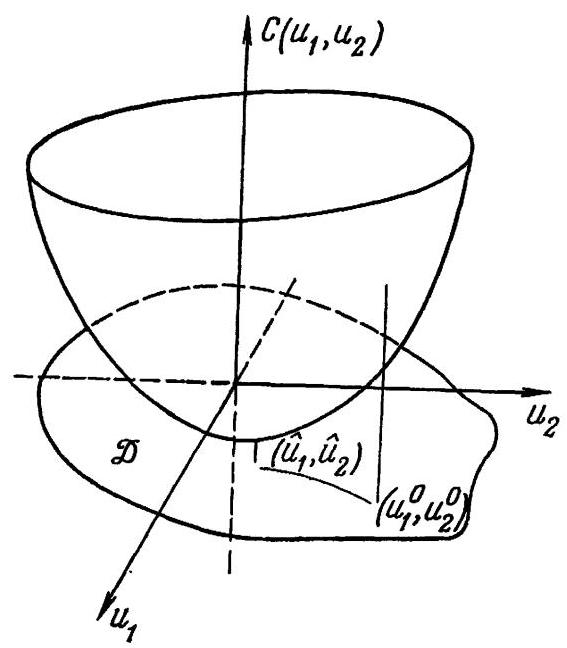
\includegraphics[max width=0.5\textwidth]{images/bo_d547k8bef24c73bgfcg0_517_882_457_567_648_0.jpg}
\end{center}
\hspace*{3em} 

Рис. А1. Траектории наискорейшего спуска в \({E}^{2}\) .

Минимизирующие значения в точке \({u}^{0}\) равны

\[
\frac{du}{ds} =  - \frac{1}{\left\lVert \begin{array}{c} \frac{\partial C}{\partial u}\left( {u}^{0}\right) \end{array} \right\rVert}\frac{\partial C}{\partial u}\left( {u}^{0}\right) .
\]

Таким образом, направление наискорейшего спуска противо- положно направлению градиента функции \(C\) в точке и,. Для того чтобы найти траекторию наиско- рейшего спуска, рассмотрим обыкновенное дифференциальное урав- henne

\[
\frac{du}{d\sigma } =  - \frac{\partial C}{\partial u}\left( u\right) ,\;u\left( 0\right)  = \left( {{u}_{1}^{0},{u}_{2}^{0}}\right) ,\;\sigma  \geq  0,
\]

обладающее решением для достаточно малых σ. Если решение предполагается единственным, то полученная пространственная кривая \(\left( {{u}_{1}\left( \sigma \right) ,{u}_{2}\left( \sigma \right) }\right)\) определяет гладкую траекторию, касатель- ная к которой в каждой точке \(\left( {{u}_{1},{u}_{2}}\right)\) совпадает с направлением наискорейшего спуска для С. Длина дуги вдоль этой кривой дается выражением

\[
s = {\int }_{0}^{\sigma }\left\lVert \begin{array}{c} {\frac{\partial C}{\partial u}\left( {u\left( \tau \right) }\right) } \end{array} \right\rVert{d\tau }\text{ и }\frac{ds}{d\sigma } = \left\lVert \begin{array}{c} {\frac{\partial C}{\partial u}\left( {u\left( \sigma \right) }\right) } \end{array} \right\rVert > 0
\]

(ds/dσ можно рассматривать, как скорость вдоль этой траектории). Вдоль этой кривой имеем

\[
\frac{dC}{d\sigma } = \frac{dC}{ds}\frac{ds}{d\sigma } =  - \left\lVert \begin{array}{c} {\frac{\partial C}{\partial u}\left( {u\left( \sigma \right) }\right) } \end{array} \right\rVert < 0,\;\text{ если }\;\frac{dC}{du} \neq  0.
\]

Поэтому функция \(C\) убывает при движении по траектории наиско- рейшего спуска, и при σ → + ∞ мы приближаемся к той точке области Ф, в которой функция \(C\) достигает минимума. В даль. нейшем будет доказана теорема, дающая достаточные условия существования единственного локального минимума, и показываю- щая, что решение дифференциального уравнения, с начальной точкой, достаточно близкой точке, в которой достигается этот минимум, стремится к этой точке при о →», если только вы- полняются некоторые локальные условия. Рассмотрим теперь за- дачу наискорейшего спуска при дополнительных ограничениях. поскольку такие ограничения часто встречаются в задачах опти- мального управления.

Пусть функции \(C\left( u\right)\) и \({g}_{i}\left( u\right) ,i = 1,2,\ldots ,r < m\) принадлежат классу \({C}^{1}\) в \(\mathcal{D} \subset  {E}^{m}\) ,и предположим,что векторы д \({g}_{i}/\partial u\) образуют линейно независимую систему в каждой точке множества Ф. Пусть и —точка из Ф, в которой grad \(C\) не равен нулю, но \({g}_{i} = 0,\;i = 1,2,\ldots ,r\) . Направление наискорейшего спуска из точки \({u}^{0}\) определяется вектором

\[
- \frac{\partial C}{\partial u} + \mathop{\sum }\limits_{{k = 1}}^{m}{\lambda }_{k}\frac{\partial {g}_{k}}{\partial u}
\]

где постоянные \({\lambda }_{k}\) определяются из системы линейных уравнений

\[
{G\lambda } = y.
\]

3aecb

\[
y = {\left\lbrack  \left\langle  \frac{\partial C}{\partial u},\frac{\partial {g}_{1}}{\partial u}\right\rangle  ,\ldots ,\left\langle  \frac{\partial C}{\partial u},\frac{\partial {g}_{m}}{\partial u}\right\rangle  \right\rbrack  }^{\prime },
\]

a \(G\) ectb mampuua \(\Gamma\) pama

\[
\left\langle  {\frac{\partial {g}_{i}}{\partial u},\frac{\partial {g}_{j}}{\partial u}}\right\rangle  ,\;i,j = 1,2,\ldots ,m,
\]

которая при принятых выше допущениях является положительно определенной. Таким образом, траектории наискорейшего спуска являются решениями дифференциального уравнения

\[
\frac{du}{d\sigma } =  - \frac{\partial C}{\partial u} + {\left( {G}^{-1}y\right) }^{\prime }\frac{\partial g}{\partial u},\;{u}^{0} = u\left( 0\right) ,\;\sigma  \geq  0.
\]

Если имеются дополнительные ограничения вида \({g}_{j}\left( u\right)  \leq  0\) , \(j = r + 1,\ldots ,r + l < m\) ,что часто случается в задачах оптималь- ного управления,— то методом, принадлежащим Вэйлентайну (Valentine), эту задачу можно свести к задаче с ограничениями в виде равенств. Это достигается введением функций

\[
{\widehat{g}}_{j}\left( {{u}_{1},\ldots ,{u}_{m},{u}_{m + 1},\ldots ,{u}_{m + l}}\right)  =
\]

\(\left. { = {g}_{j}{u}_{1},\ldots ,{u}_{m}}\right)  + {\left( {u}_{m + j - r}\right) }^{2} = 0\) для \(j = r + 1,\ldots ,r + l\)

и, кроме того, заменой исходной функции \(C\) функцией \(\widehat{C}\) по фор- муле \(\widehat{C}\left( {{u}_{1},\ldots ,{u}_{m},{u}_{m + l}}\right)  = C\left( {{u}_{1},\ldots ,{u}_{m}}\right)\) . Tem самым,исходная задача сводится к задаче минимизации функции С в Евг-1 при ограничениях

\[
{g}_{i}\left( {{u}_{1},\ldots ,{u}_{m}}\right)  = 0,\;i = 1,2,\ldots ,r,
\]

\[
{\widehat{g}}_{j}\left( {{u}_{1},\ldots ,{u}_{m + l}}\right)  = 0,\;j = r + 1,\ldots ,r - 1.
\]

Далее мы будем рассматривать задачу наискорейшего спуска в функциональном пространстве; полученные при этом результаты относительно сходимости будут верны также и для пространств конечной размерности. Прежде чем применить метод наискорей- шего спуска к функционалам, определенным на некотором функ- циональном пространстве, необходимо уточнить понятие градиента (см. также упражнения раздела 6.1). Для этого нам придется развить некоторые методы функционального анализа. Все ниже- следующие результаты имеются в главе 6 книги Люстерника и Соболева. Прежде всего введем понятие длины в банаховом про- странстве.

Пусть U — действительное банахово пространство с нормой \(\left| \cdot \right|\) ; рассмотрим функцию \(u\left( t\right)\) ,заданную на конечном интервале \(a \leq  t \leq  b\) , и принимающую значения из U. Функция и (t) называется непре- рывной на \(\left\lbrack  {a,b}\right\rbrack\) , если она непрерывно отображает отрезок \(\left\lbrack  {a,b}\right\rbrack\) в пространство U с топологией, индуцированной на нем его нор- мой. Функция \(u\left( t\right)\) непрерывно дифференцируема на \(\left\lbrack  {a,b}\right\rbrack\) , если имеется элемент \({u}^{\prime }\left( t\right)  \in  U\) ,такой,что

\[
\mathop{\lim }\limits_{{{\Delta t} \rightarrow  0}}\left| {\frac{u\left( {t + {\Delta t}}\right)  - u\left( t\right) }{\Delta t} - {u}^{\prime }\left( t\right) }\right|  = 0
\]

для любого \(t \in  \left\lbrack  {a,b}\right\rbrack\) . На концах интервала рассматриваются од- носторонние производные. (Более общие определения можно найти в книге Хилле и Филлипса, глава 3.)

Рассмотрим некоторое разбиение интервала [a, b], \({\pi }_{m} : a \leq \; \leq  {t}_{0} \leq  {t}_{1} \leq  \ldots  \leq  {t}_{m} = b\) и положим

\[
S\left( {u,{\pi }_{m}}\right)  = \mathop{\sum }\limits_{{i = 1}}^{m}\left| {u\left( {t}_{i}\right)  - u\left( {t}_{i - 1}\right) }\right| .
\]

Непрерывная кривая в И, определяемая функцией и (t), называется спрямляемой, если для нее величина \(L = \sup S\left( {u,{\pi }_{n}}\right)\) , конечна. Здесь супремум берется по всем конечным разбиениям интервала \(\left\lbrack  {a,b}\right\rbrack\) . Если, кроме того, \({u}^{\prime }\left( t\right)\) непрерывна и \(\left| {{u}^{\prime }\left( t\right) }\right|  \neq  0\) для \(t \in  \left\lbrack  {a,b}\right\rbrack\) , то \(u\left( t\right)\) называется гладкой кривой. Если и (t) — гладкая кривая, то можно показать, что длина дуги ее вычисляется, как и в пространстве \({E}^{m}\) ,по формуле

\[
s = {\int }_{0}^{t}\left| {{u}^{\prime }\left( \sigma \right) }\right| {d\sigma }
\]

Отсюда видно, что если параметром в параметрическом представ- лении кривой является длина дуги, то \(\left| {{u}^{\prime }\left( t\right) }\right|  = 1\) . Справедливо и обратное утверждение.

Например, если \(U = {L}_{2}\left\lbrack  {0,1}\right\rbrack\) , где \({L}_{2}\left\lbrack  {0,1}\right\rbrack\) есть пространство функций, интегрируемых с квадратом, то для гладкой кривой и (я, о), \(0 \leq  \sigma  \leq  1\) выполняется соотношение

\[
{\int }_{0}^{1}{\left( \frac{\partial u}{\partial s}\left( s,\sigma \right) \right) }^{2}{ds} = 1,\text{ где }\frac{\partial u}{\partial s}\left( {s,\sigma }\right)  = {u}^{\prime }\left( s\right) .
\]

Этот факт весьма важен для применения метода наискорейшего спуска к задаче минимизации функционала.

Важным понятием в методе наискорейшего спуска является также понятие производной Фреше. Мы дадим здесь определение этого понятия в форме, достаточно общей для наших целей. Обо- значим через \% действительное гильбертово пространство со ска- лярным произведением <., .); пространство действительных чисел обозначим символом R. Пусть С есть некоторая функция С: Ж — R, и пусть \({u}_{0},h \in  \mathcal{H}\) . Говорят, что функция С имеет дифференциал Фреше (или сильный дифференциал) С’(и) h, если существует такой непрерывный линейный функционал \({C}^{\prime }\left( {u}_{0}\right)\) на \(\mathcal{H}\) ,что

\[
\left| {C\left( {{u}_{0} + h}\right)  - C\left( {u}_{0}\right)  - {C}^{\prime }\left( {u}_{0}\right) h}\right|  = o\left( {\parallel h\parallel }\right) ,
\]

при \(\parallel h\parallel  \rightarrow  0\) ,где || \(h\parallel  = {\left( \langle h,h\rangle \right) }^{1/2}\) . Функция \(g\left( h\right)\) обозначается символом \(o\left( {\parallel h\parallel }\right)\) , если \(\frac{\left| g\left( h\right) \right| }{\parallel h\parallel } \rightarrow  0\) при \(\parallel h\parallel  \rightarrow  0\) . Линейный функ- ционал \({C}^{\prime }\left( {u}_{0}\right)\) называется производной Фреше функции \(C\) в точке \({u}_{0}\) . Выражение

\[
{DC}\left( {{u}_{0},h}\right)  = {\left. \frac{\partial C}{\partial \lambda }\left( {u}_{0} + \lambda h\right) \right| }_{\lambda  = 0} = \mathop{\lim }\limits_{{\lambda  \rightarrow  0}}\frac{C\left( {{u}_{0} + {\lambda h}}\right)  - C\left( u\right) }{\lambda },
\]

если оно существует, называется производной по направлению, или слабым дифференциалом функции С в точке и... Если слабый диф- ференциал обладает некоторыми определенными свойствами, то \(\dot{DC}\left( {{u}_{0},h}\right)  = {C}^{\prime }\left( {u}_{0}\right) h\) ,что дает возможность вычислить производную Фреше. Эти свойства выражаются следующей теоремой:

Теорема 1. Ecnu производная по направлению DC \(\left( {u,h}\right)\) cy- ществует при  \textbackslash u \textbackslash u \textbackslash u \textbackslash u \textbackslash eu ∈а, а х о, и если она равномерно непре- рывна по и и непрерывна по h, то тогда существует дифференциал Фреше, и С'(и) h = DC (и, h). (Доказательство см. в главе 6 книги Люстерника и Соболева.)

Аналогично определяются производные Фреше высших поряд. ков. Обозначим через \({\mathcal{H}}^{ * }\) банахово пространство непрерывных линейных функционалов на \(\mathcal{H}\) с нормой \({\left| \cdot \right| }_{1}\) . Говорят, что функ- ция \(C\) ,имеющая производную Фреше, имеет второй дифференциал Фреше C" (ио) h, если

\[
{\left| {C}^{\prime }\left( {u}_{0} + h\right)  - {C}^{\prime }\left( {u}_{0}\right)  - {C}^{\prime \prime }\left( {u}_{0}\right) h\right| }_{1} = o\left( {\parallel h\parallel }\right)
\]

при \(\parallel h\parallel  \rightarrow  0.{C}^{\prime \prime }\left( {u}_{0}\right)\) есть непрерывный линейный оператор, пере- водящий \% в \%*. Применив теорему 1, можно показать, что если вторая производная по направлению

\[
{\left. \frac{{\partial }^{2}C}{\partial {\lambda }_{1}\partial {\lambda }_{2}}\left( {u}_{0} + {\lambda }_{1}h + {\lambda }_{2}{h}_{1}\right) \right| }_{\begin{array}{c} {{\lambda }_{1} = 0} \\  {{\lambda }_{2} = 0} \end{array}},{u}_{0},\lambda ,{h}_{1} \in  \mathcal{H}
\]

удовлетворяет всем условиям непрерывности, то

\[
\left( {{C}^{\prime \prime }\left( {u}_{0}\right) {h}_{1}}\right) h = {\left. \frac{{\partial }^{2}C}{\partial {\lambda }_{1}\partial {\lambda }_{2}}\left( {u}_{0} + {\lambda }_{1}h + {\lambda }_{2}{h}_{1}\right) \right| }_{\begin{array}{c} {{\lambda }_{1} = 0} \\  {{\lambda }_{2} = 0} \end{array}}.
\]

Оператор \({C}^{\prime \prime }\left( u\right)\) называется второй производной Фреше.

Пусть функция \(C\) удовлетворяет тем же условиям, что и рань- ше, и предположим, что она обладает непрерывными первой и вто- рой производной Фреше в Ж. Первая производная Фреше есть линейный функционал на \%, и по теореме Рисса имеет представ- ление

\[
{C}^{\prime }\left( u\right) h = \left\langle  {\frac{\partial C}{\partial u}\left( u\right) ,h}\right\rangle  ,\;h \in  \mathcal{H},
\]

где \(\left( {\partial C/\partial u}\right) \left( u\right)\) —однозначно определенный элемент \#. Элемент \(\left( {\partial C/\partial u}\right) \left( u\right)\) называется градиентом функции С в точке и. Это оп- ределение совпадает с определением градиента в пространстве ко- нечной размерности \({E}^{n}\) . Поскольку \({C}^{\prime \prime }\left( u\right) h\) есть также непрерывный линейный функционал на \(\mathcal{H}\) , то по теореме Рисса

\[
\left( {{C}^{\prime \prime }\left( u\right) h}\right) h = \left\langle  {{H}_{C}\left( u\right) h,h}\right\rangle  ,
\]

где \({H}_{C}\left( u\right)\) есть непрерывный линейный оператор на \(\mathcal{H}.{H}_{C}\left( u\right)\) называется гессианом функции \(C\) в точке и. Для пространств ко- нечной размерности \({H}_{c}\left( u\right)\) сводится к симметрической матрице вторых частных производных функции С.

Основным пространством в наших рассуждениях до сих пор было гильбертово пространство Ж. Это требование можно несколько ослабить. Пусть U—линейное топологическое пространство с опре- деленным на нем скалярным произведением </, ·); обозначим через \(\bar{U}\) ero пополнение в метрике \(d\left( {u,y}\right)  = \parallel u - y\parallel  = \langle u - y,u - y{\rangle }^{1/2}\) . Пусть C —действительная функция на U, имеющая производную Фреше C′ (и). По теореме Рисса о представлении существует един- ственный элемент \({C}_{u} \in  \bar{U}\) ,такой,что \({C}^{\prime }\left( u\right) h = \left\langle  {{C}_{u},h}\right\rangle  ,h \in  \bar{U}\) . Если \({C}_{u} \in  U\) , то \({C}_{u}\) называется градиентом функции \(C\sharp \left( {\partial C/\partial u}\right) \left( u\right)  = {C}_{u}\) . Функция \(C\) может не обладать градиентом для каждого \(u \in  U\) . Поэтому в пространстве U часто приходится заменять имеющуюся там норму более слабой и рассматривать пополнение простран- ства U по этой норме. При этом новая норма выбирается так, чтобы функция \(C\) имела градиент в любой точке и из пополнения. Так, например, вместо банахова пространства действительных непрерывных функций на интервале I удобнее рассматривать его пополнение по норме

\[
{\left( {\int }_{I}{u}^{2}d\mu \right) }^{1/2}
\]

т. е. гильбертово пространство интегрируемых с квадратом по Лебегу функций со скалярным произведением \({\int }_{i}{uyd\mu }\) .

Будем теперь рассматривать метод наискорейшего спуска для функций, определенных на гильбертовом пространстве Ж. Пусть \(C\) —действительнозначная функция, определенная на \#, и имеющая непрерывную первую производную Фреше. Пусть и не не и на усть \(\gamma  -\) гладкая кривая в Ж, проходящая через и. Если за параметр принять длину дуги кривой, то || \({u}^{\prime }\left( s\right) {\parallel }^{2} = 1\) и

\[
\frac{dC}{ds} = \mathop{\lim }\limits_{{{\Delta s} \rightarrow  0}}\frac{C\left( {u\left( {s + {\Delta s}}\right) }\right)  - {C}^{\prime }\left( {u\left( s\right) }\right) }{\Delta s} = \left\langle  {\frac{\partial C}{\partial u}\left( {u\left( s\right) }\right) ,{u}^{\prime }\left( s\right) }\right\rangle  .
\]

Направление наискорейшего спуска есть направление, минимизи- рующее функционал

\[
\left\langle  {\frac{\partial C}{\partial u}\left( {u}_{1}\right) ,{u}^{\prime }\left( 0\right) }\right\rangle
\]

при ограничении

\[
{\left\lVert \begin{array}{c} {u}^{\prime }\left( 0\right) \end{array} \right\rVert}^{2} = 1.
\]

Здесь мы умышленно сохранили обозначения, использованные нами в конечномерном случае, так как все сформулированные выше результаты для \({E}^{n}\) переносятся и на бесконечномерный случай, конеч- но, в соответствующей интерпретации. Траектория наискорейшего спуска находится как решение дифференциального уравнения

\[
\frac{du}{d\sigma } =  - \frac{\partial C}{\partial u}\left( u\right) ,\;u\left( 0\right)  = {u}_{1} \in  \mathcal{H},\sigma  \geq  0.
\]

Решение является функцией со значениями в \%, и вдоль этой траектории функция \(C\left( {u\left( \sigma \right) }\right)\) убывает,так как

\[
\frac{d{C}_{1}}{d\sigma } = \left\langle  {\frac{\partial C}{\partial u},\frac{du}{d\sigma }}\right\rangle   =  - {\left\lVert \begin{array}{c} \frac{\partial C}{\partial u}\left( u\left( \sigma \right) \right) \end{array} \right\rVert}^{2} < 0
\]

при \(\partial C/\partial u \neq  0\) . Это вытекает из следующих теорем, принадлежа- щих Розенблюму. В этих теоремах С есть действительнозначная функция, определенная на гильбертовом пространстве Ж.

Теорема 2. Пусть функция С имеет две непрерывные про- изводные Фреше в некоторой выпуклой области D пространства H, \(u\) nycm \(b\) cpea \(S\left( u\right)  = \left\{  {u \mid  u \in  \mathcal{H},\left\lVert \begin{array}{c} {u - {u}_{0}} \end{array} \right\rVert \leq  a \mid  A}\right\}\) ,где \(a = \left\lVert \begin{array}{c} {\frac{\partial C}{\partial u}\left( {u}_{0}\right) } \end{array} \right\rVert\) , а константа А определяется ниже, содержится в D. Далее, пред- положим, что

\[
\left\langle  {{H}_{C}\left( u\right) v,v}\right\rangle   \geq  A\parallel v{\parallel }^{2},
\]

при \(u \in  D,v \in  \mathcal{H}u\) фиксированном \(A > 0,u\) что функция \(u\left( \sigma \right)\) удовлетворяет уравнению

(*)
\[
\frac{du}{d\sigma }\left( \sigma \right)  =  -  - \frac{\partial C}{\partial u}\left( {u\left( \sigma \right) }\right)
\]

\(\left( {\partial n * \sigma  \geq  0,u\left( 0\right)  = {u}_{0} \in  D}\right) .{H}_{C}\left( u\right)\) есть гессиан функции C в точке и. Tozda:

a) \(\theta \mathcal{H}\) cyществуют пределы: \(\mathop{\lim }\limits_{{\sigma  \rightarrow  \infty }}u\left( \sigma \right)  = {u}_{\infty }\) ;

b) \(\mathop{\lim }\limits_{{\sigma  \rightarrow  \infty }}C\left( {u\left( \sigma \right) }\right)  = c\) ;

\(u,\kappa\) pome mozo,

c) \(\left\lVert \begin{array}{c} {u\left( \sigma \right)  - {u}_{\infty }} \end{array} \right\rVert \leq  \left( {a/A}\right) \exp \left( {-{A\sigma }}\right)\) ,

\[
0 \leq  C\left( {u\left( \sigma \right) }\right)  - c \leq  \frac{{a}^{2}}{2A}\exp \left( {-{2A\sigma }}\right) ,
\]

\(u\partial n\mathcal{A}\theta\) cc \(x\;u \in  D\)

\[
C\left( u\right)  \geq  c + \frac{A}{2}{\left\lVert \begin{array}{c} u - {u}_{\infty } \end{array} \right\rVert}^{2}.
\]

Таким образом, если выполнены все предположения теоремы 2 то метод наискорейшего спуска гарантирует экспоненциальную сходимость соответствующей последовательности значений функ- ции С к минимальному значению. Из пункта а) следует, что ми- нимизирующий элемент определен однозначно. Заметим также, что решение уравнения (*) должно существовать при всех неотрица- тельных σ, что в некоторых случаях довольно сложно проверить. В статье Розенблюма получено несколько достаточных условий существования решения для всех σ. Одно из наиболее простых условий состоит в том, чтобы производная дС/ди удовлетворяла условию Липшица внутри шара \(S\left( u\right)\) ,откуда следует,что

\[
\mathop{\lim }\limits_{{\sigma  \rightarrow  \infty }}\left\lVert \begin{array}{c} {\frac{\partial C}{\partial u}\left( {u\left( \sigma \right) }\right) } \end{array} \right\rVert = 0.
\]

Метод наискорейшего спуска может быть использован для реше- ния некоторых изопериметрических задач. Для простоты рассмотрим задачу нахождения минимума функции \(C\) на \(\mathcal{H}\) ,при дополни- тельном условии g=0. Траектория наискорейшего спуска опре- деляется из уравнений

(**)
\[
\frac{du}{d\sigma } =  - \frac{\partial C}{\partial u} + \lambda \left( u\right) \frac{\partial g}{\partial u},\;\lambda \left( u\right)  = \frac{\left\langle  \frac{\partial C}{\partial u},\frac{\partial g}{\partial u}\right\rangle  }{{\left\lVert \begin{array}{c} \frac{\partial g}{\partial u} \end{array} \right\rVert}^{2}}
\]

\({\text{ п }\text{ р }\text{ и }}\;{\text{ у }\text{ с }\text{ л }\text{ о }\text{ в }\text{ н }\text{ н }},\;{\text{ ч }\text{ т }\text{ о }}\;\left\lVert \begin{array}{c} \frac{\partial g}{\partial u} \end{array} \right\rVert \neq  0.\;{\text{ П }\text{ р }\text{ н }}\;{\text{ т }\text{ а }\text{ к }\text{ о }\text{ м }}\;{\text{ в }\text{ ы }\text{ б }\text{ о }\text{ р }\text{ е }}\;{\text{ т }\text{ р }\text{ а }\text{ е }\text{ к }\text{ т }\text{ о }\text{ р }\text{ н }\text{ и }}\)

\[
\frac{dC}{d\sigma } =  - \left\{  \frac{\left\lVert \begin{array}{c} \frac{\partial C}{\partial u} \end{array} \right\rVert\left\lVert \begin{array}{c} \frac{\partial g}{\partial u} \end{array} \right\rVert - \left\langle  {\frac{\partial C}{\partial u},\frac{\partial g}{\partial u}}\right\rangle  }{{\left\lVert \begin{array}{c} \frac{\partial g}{\partial u} \end{array} \right\rVert}^{2}}\right\}   < 0,\;\frac{{dg}\left( u\right) }{d\sigma } = 0.
\]

Следующая теорема, также принадлежащая Розенблюму, дает достаточные условия для того, чтобы метод наискорейшего спуска определял единственное решение этой задачи.

Теорема 3. Пусть функции С и д имеют по две непрерыв- ные производные Фреше в некоторой выпуклой области D прост- ранства H, и пусть м есть многообразие, определенное равенст- вом \(g\left( u\right)  = 0,u \in  D\) . Предположим, что дд/ди ≠ 0 на A и что

\[
\left\langle  {\left( {{H}_{C}\left( u\right)  - \lambda \left( u\right) {H}_{g}\left( u\right) }\right) v,v}\right\rangle   \leq  A\parallel v{\parallel }^{2},\;A > 0
\]

\({при}\;u \in  \mathcal{M},v \in  \mathcal{H},\langle \partial g\left( u\right) /\partial u,v\rangle  = 0.{\Pi ycmb}\;k\left( u\right)  - {paccmo\text{ я }\text{ н }\text{ и }e}\) от точки и до границы многообразия м, и пусть E — множество точек и, ес м таких, что

\[
a\left( {u}_{0}\right)  = \left\lVert \begin{array}{c} {\frac{\partial C\left( u\right) }{\partial u} - \lambda \left( {u}_{0}\right) \frac{\partial g\left( {u}_{0}\right) }{\partial u}} \end{array} \right\rVert < {Ak}\left( {u}_{0}\right) ,
\]

и таких, что решение системы (**) при и (0) = и。существует при всех σ ≥0. Тогда для всех и в Е решение и (σ) обладает все- ми свойствами, сформулированными в теореме 2. Более того, если точки \({u}_{0}\) и \({u}_{0}\) из \(E\) можно соединить дугой класса \({C}^{1}\) в Е,то \({u}_{\infty } = {\widetilde{u}}_{\infty },u,\) наконец, echu \(c = \mathop{\lim }\limits_{{\sigma  \rightarrow  \infty }}C\left( {u\left( \sigma \right) }\right)\) при \(u\left( 0\right)  = {u}_{0} \in  E,\) mo

\[
C\left( {u}_{0}\right)  \geq  c + \frac{4{A}^{2}{\delta }^{3}}{27a}\left( {1 + \frac{A\delta }{3a}}\right) ,\;\delta  = \left\lVert \begin{array}{c} {{u}_{0} - {u}_{\infty }} \end{array} \right\rVert,\;a = a\left( {u}_{0}\right) .
\]

Теорема верна и при наличии нескольких дополнительных условий.

До сих пор мы занимались вопросом о том, как построить траекторию наискорейшего спуска, базируясь на локальной гра- диентной информации относительно функции (или функционала) \(C\left( u\right)\) . Пользуясь такой информацией, можно получить решение дифференциального уравнения, дающее траекторию наискорейшего спуска, в конечномерном случае с помощью аналоговой вычисли- тельной машины. Однако чаще применение метода наискорейшего спуска осуществляется с помощью цифровых вычислительных устройств. При этом итерация производится по формуле

\[
{u}_{k + 1} = {u}_{k} - {\rho }_{k}\nabla C\left( {u}_{k}\right) ,\;{\rho }_{k} > 0,
\]

где \(k = 0,1,2,\ldots\) Таким образом,машина вычисляет изменение \(u\) на \(k + 1\) -м шаге, в зависимости от первоначального значения и и от значения градиента ∇C на k-м шаге. Результаты применения этого метода можно найти в работах Голдстайна (Goldstein).

На этом мы закончим введение в метод наискорейшего спуска и приступим к приложениям этого метода в задачах оптимального управления.

\section*{А2. Применение метода наискорейшего спуска к задачам оптимального управления и формулировка вычислительных алгоритмов}

В этом разделе мы займемся применением метода наскорейшего спуска к задачам оптимального управления. Вначале, в приме- pax 1-3, будет показано, что метод наискорейшего спуска можно считать конструктивным подходом к задачам оптимального управ- ления, удовлетворяющим, например, необходимым условиям, типа тех, которые выводятся из принципа максимума. Затем в приме- рах 4—7 мы покажем, как можно получить вычислительные алго- ритмы для отыскания оптимальных управлений. Один из подхо- дов — прямой, в другом используется принцип максимума, с по- мощью которого определяется вид оптимального управления как функции от параметров, а затем система параметров корректи- руется методом наискорейшего спуска. Примеры 4—7 доводятся лишь до той стадии, когда становится ясным соответствующий алгоритм вычислений на машине, и поэтому не могут считаться завершенными.

Пример 1. Рассмотрим линейную управляемую систему первого порядка,

\[
\dot{x} = {ax} + u\left( t\right) ,
\]

со скалярным управлением \(u\left( t\right)\) и фундаментальной матрицей \({\Phi }^{-1}\left( t\right)  = {e}^{at}\) на интервале [0, \(T\rbrack\) c \(x\left( 0\right)  = 0,\Phi \left( 0\right)  = 1\) и фиксиро- ванным \(T > 0\) . Задача оптимального управления состоит в том, чтобы перевести систему из точки \(x\left( 0\right)  = {x}_{0} = 0\) в точку \(x = {\Phi }^{-1}\left( T\right) c\) для некоторого постоянного \(c\) ,за время \(T\) , \(c\) минимальным зна- чением критерия качества

\[
C\left( u\right)  = {\int }_{0}^{T}{\left( u\left( t\right) \right) }^{2}{dt}
\]

Как и в аналогичных задачах главы 3, потребуем, чтобы ие \(\in  {L}_{2}\left\lbrack  {0,T}\right\rbrack\) ,где \({L}_{2}\left\lbrack  {0,T}\right\rbrack\) обозначает гильбертово пространство функций, интегрируемых с квадратом по Лебегу на интервале [0, \(T\) ]. Таким образом, задача состоит в минимизации выра- жения

\[
{\int }_{0}^{T}{u}^{2}\left( t\right) {dt}
\]

прн ограниченин

\[
{\int }_{0}^{T}\Phi \left( t\right) u\left( t\right) {dt} =  : c,
\]

где и скалярная функция из \({L}_{2}\left\lbrack  {0,T}\right\rbrack  ,\Phi \left( t\right)  \in  {L}_{2}\left\lbrack  {0,T}\right\rbrack\) , a \(c -\) заданная константа. Если се 0, то и = 0 есть оптимальное реше- ние. Заметим, что \(\parallel \Phi \parallel  \neq  0\) . В обозначениях теорем 2 и 3 имеем

\[
C\left( u\right)  = {\int }_{0}^{T}{u}^{2}\left( t\right) {dt};\;g\left( u\right)  = {\int }_{0}^{T}\Phi \left( t\right) u\left( t\right) {dt} - c.
\]

Вычислим теперь градиенты функций C и g. Рассмотрим их про- изводные по направлению

\[
{\left. \frac{\partial C}{\partial \lambda }\left( u + \lambda z\right) \right| }_{\lambda  = 0} = {\int }_{0}^{T}{2u}\left( t\right) z\left( t\right) {dt},
\]

и

\[
{\left. \frac{\partial g}{\partial \lambda }\left( u + \lambda z\right) \right| }_{\lambda  = 0} = {\int }_{0}^{T}\Phi \left( t\right) z\left( t\right) {dt},\;z \in  {L}_{2}\left\lbrack  {0,T}\right\rbrack  .
\]

В силу того, что ограниченные линейные функционалы на \({L}_{2}\left\lbrack  {0,T}\right\rbrack\) обладают представлением \({\int }_{0}^{T}\psi \left( t\right) z\left( t\right) {dt}\) для некоторого фиксиро- ванного \(\psi  \in  {L}_{2}\left\lbrack  {0,T}\right\rbrack\) , to мы видим,что

\[
\frac{\partial C}{\partial u} = {2u}\;\text{ и }\;\frac{\partial g}{\partial u} = \Phi .
\]

Для того чтобы вычислить гессианы функций С и g, рассмотрим их вторые производные по направлению

\[
{\left. \frac{{\partial }^{2}C}{\partial {\lambda }^{2}}\left( u + \lambda z\right) \right| }_{\lambda  = 0} = {\int }_{0}^{T}2{z}^{2}\left( t\right) {dt}
\]

\[
{\left. \frac{{\partial }^{2}g}{\partial {\lambda }^{2}}\left( u + \lambda z\right) \right| }_{\lambda  = 0} = 0.
\]

Гессиан функции С является непрерывным линейным оператором

\[
{H}_{C}\left( u\right) z = {2z},\;z \in  {L}_{2}\left\lbrack  {0,T}\right\rbrack
\]

a reссиан функцин g есть нулевой оператор

\[
{H}_{g}\left( u\right) z = 0,\;z \in  {L}_{2}\left\lbrack  {0,T}\right\rbrack  .
\]

Покажем теперъ, что выполнены условия теоремы 3. Поскольку

\[
\left\langle  {\left( {{H}_{C}\left( u\right)  - \lambda \left( u\right) {H}_{g}\left( u\right) }\right) v,v}\right\rangle   = \left\langle  {{H}_{C}\left( u\right) v,v}\right\rangle   = 2\parallel v{\parallel }^{2},
\]

то \(A = 2\) . Если точки иоийлежат Е,т. е.,если

\[
{\int }_{0}^{T}\Phi \left( t\right) {u}_{0}\left( t\right) {ds} = c,\;{\int }_{0}^{T}\Phi \left( t\right) {\widetilde{u}}_{0}\left( t\right) {dt} = c,
\]

то функция \(\widehat{u} = \mu {u}_{0} + \left( {1 - \mu }\right) {\widetilde{u}}_{0},\;0 \leq  \mu  \leq  1\) ,представляет собой кривую класса \({C}^{1}\) в \(E\) , coeдиняющую точки \({u}_{0}\) и \({\widetilde{u}}_{0}\) . Cледова- тельно, если решение существует, то оно единственно.

\[
\text{ Mhoжество }B = \left\{  {u\left| {\;u \in  {L}_{2}\left\lbrack  {0,T}\right\rbrack  }\right. ,{\int }_{0}^{T}\Phi \left( t\right) u\left( t\right) {dt} = c}\right\}  \;\text{ представ- }
\]

ляет собой гиперплоскость, и значит, условие

\[
a\left( {u}_{0}\right)  < {Ak}\left( {u}_{0}\right)
\]

теоремы 3 выполняется для любого элемента из многообразия м (см. теорему 3). Функция и, удовлетворяющая уравнению g(и\_0) = 0, может быть найдена из определенного выше уравнения, если использовать ступенчатые функции.

Дифференциальное уравнение, определяющее функцию \(u\left( \mathfrak{o}\right)\) из теоремы 3, имеет вид

\[
\frac{du}{d\sigma } =  - {2u} + \lambda \left( u\right) \Phi ,\;u\left( 0\right)  = {u}_{0},\;\sigma  \geq  0.
\]

Но поскольку

\[
\lambda \left( u\right)  = \frac{\left\langle  \frac{\partial C}{\partial u},\frac{\partial g}{\partial u}\right\rangle  }{\parallel \Phi {\parallel }^{2}} = \frac{2{\int }_{0}^{T}\Phi \left( t\right) u\left( t\right) {dt}}{\parallel \Phi {\parallel }^{2}} = \frac{2c}{\parallel \Phi {\parallel }^{2}},
\]

ТО

\[
\frac{du}{d\sigma }\left( {t,\sigma }\right)  =  - {2u}\left( {t,\sigma }\right)  + \frac{2c}{\parallel \Phi {\parallel }^{2}}\Phi \left( t\right) ,
\]

\[
0 \leq  t \leq  T,\;0 \leq  \sigma ,\;u\left( {t,0}\right)  = {u}_{0}\left( t\right) .
\]

Решенне этого линейного уравнения дается выражением

\[
u\left( {t,\sigma }\right)  = {e}^{-{2\sigma }}{u}_{0}\left( t\right)  + \frac{{c\Phi }\left( t\right) }{\parallel \Phi {\parallel }^{2}}\left( {1 - {e}^{-{2\sigma }}}\right) .
\]

Такнм образом, по теореме 3, единственным миннииянрующим элементом является

\[
{u}_{\infty }\left( t\right)  = \frac{c}{\parallel \Phi {\parallel }^{2}}\Phi \left( t\right)
\]

a \(C\left( {u}_{\infty }\right)  = {c}^{2}\) . Этот же результат можно получить, используя необ- ходимые условия, вытекающие из принципа максимума так же, как в главе 3.

Пример 2. Рассмотрим линейную управляемую систему

\[
{\dot{x}}^{1} = a{x}^{1} + u\left( t\right) ,\;{\dot{x}}^{2} = b{x}^{2} + u\left( t\right)
\]

со скалярным управлением и (t) и a ≠ b. Задача оптимального управления состоит в том, чтобы перевести систему с выходом \({x}^{1}\left( t\right)\) из точки \({x}^{1}\left( 0\right)  = 0\) в точку \({x}^{1} = {\Phi }_{1}{}^{-1}\left( T\right) c\) ,для некоторого постоянного \(c\) ,при минимальном значении критерия качества

\[
C\left( u\right)  = {\left( {\int }_{0}^{T}{\Phi }_{2}\left( t\right) u\left( t\right) dt\right) }^{2} + {\int }_{0}^{T}{\left( u\left( t\right) \right) }^{2}{dt},
\]

где T-фиксированное положительное число, а фундаментальная матрица

\[
\psi \left( t\right)  = \left[ \begin{array}{cc} {\Phi }_{1}^{-1}\left( t\right) & 0, \\  0 & {\Phi }_{2}^{-1}\left( t\right) \end{array} \right]
\]

удовлетворяет условию

\[
\psi \left( 0\right)  = \left\lbrack  \begin{array}{ll} 1 & 0 \\  0 & 1 \end{array}\right\rbrack
\]

Таким образом, мы рассматриваем здесь задачу минимизации функционала

\[
{\left( {\int }_{0}^{T}{\Phi }_{2}\left( t\right) u\left( t\right) dt\right) }^{2} + {\int }_{0}^{T}{u}^{2}\left( t\right) {dt}
\]

при дополнительном ограничении

\[
{\int }_{0}^{T}{\Phi }_{1}\left( t\right) u\left( t\right) {dt} = c
\]

Функции \({\Phi }_{2}\left( t\right)\) и \({\Phi }_{1}\left( t\right)\) принадлежат пространству \({L}_{2}\left\lbrack  {0,T}\right\rbrack\) , \({\Phi }_{1} \neq  {\Phi }_{2}\) и \(\left\lVert \begin{array}{c} {\Phi }_{1} \end{array} \right\rVert \neq  0.\) 3 десь \(C\left( u\right)  = {\left( {\int }_{0}^{T}{\Phi }_{2}\left( t\right) u\left( t\right) dt\right) }^{2} + {\int }_{0}^{T}{u}^{2}\left( t\right) {dt}\) ; обозначая \(g\left( u\right)  = {\int }_{0}^{T}{\Phi }_{1}\left( t\right) u\left( t\right) {dt} - c\) ,вычислим производные функ- ций \(C\) и \(g\) по направлению:

\[
\frac{\partial C}{\partial u} = 2{\int }_{0}^{T}{\Phi }_{2}\left( \tau \right) u\left( \tau \right) {d\tau }{\Phi }_{2}\left( t\right)  + {2u}\left( t\right)
\]

II

\[
\frac{\partial g}{\partial u} = {\Phi }_{1}\left( t\right)
\]

Аналогичное вычисление показывает, что

\[
{H}_{C}\left( u\right) z = 2{\int }_{0}^{T}{\Phi }_{2}\left( \tau \right) z\left( \tau \right) {d\tau }{\Phi }_{2}\left( t\right)  + {2z}\left( t\right) ,
\]

\[
{H}_{g}\left( u\right) z = 0,\;z \in  {L}_{2}\left\lbrack  {0,T}\right\rbrack  .
\]

Поскольку

\[
\left. {\left\langle  {\left( {{H}_{C}\left( u\right)  - \lambda \left( u\right) {H}_{g}\left( u\right) }\right) v,v}\right)  = }\right\rangle
\]

\[
= 2{\left( {\int }_{0}^{T}{\Phi }_{2}\left( \tau \right) v\left( \tau \right) d\tau \right) }^{2} + 2\langle v,v\rangle  \geq  2\langle v,v\rangle ,
\]

то, пользуясь теоремой 3, заключаем, что единственное оптималь- ное решение может быть найдено из дифференциального уравнения

\[
\frac{du}{d\sigma } =  - \frac{\partial C}{\partial u} + \lambda \left( u\right) \frac{\partial g}{\partial u},\;\Gamma \text{ дel }\;u\left( 0\right)  = {u}_{0},\;\sigma  \geq  0,
\]

\[
\lambda \left( u\right)  = \frac{{2c} + 2\left\langle  {{\Phi }_{2},{\Phi }_{1}}\right\rangle  \mathop{\int }\limits_{0}^{T}{\Phi }_{2}\left( \tau \right) u\left( {\tau ,\sigma }\right) {d\tau }}{{\left\lVert \begin{array}{c} {\Phi }_{1} \end{array} \right\rVert}^{2}},
\]

которое может бытъ приведено к виду

\[
\frac{du}{d\sigma }\left( {t,\sigma }\right)  =  - {2u}\left( {t,\sigma }\right)  - 2{\int }_{0}^{T}{\Phi }_{2}\left( \tau \right) u\left( {\tau ,\sigma }\right) {d\tau }{\Phi }_{2}\left( t\right)  +
\]

\[
+ \left\{  {2\left\langle  {{\Phi }_{2},{\Phi }_{1}}\right\rangle  {\int }_{0}^{T}{\Phi }_{2}\left( \tau \right) u\left( {\tau ,\sigma }\right) {d\tau } + {2c}}\right\}  \frac{{\Phi }_{1}\left( t\right) }{{\left\lVert \begin{array}{c} {\Phi }_{1} \end{array} \right\rVert}^{2}},
\]

\[
u\left( {t,0}\right)  = {u}_{0}\left( t\right) ,\;\sigma  \geq  0.
\]

Это дифференциальное уравнение имеет единственное решение при всех σ=>0, поскольку оно удовлетворяет условию Липшица в \({L}_{2}\left\lbrack  {0,T}\right\rbrack\) . Пользуясь теоремой 3, находим единственное опти- мальное решение и (t) нашей задачи. Пользуясь неравенством Шварца и учитывая замечание, сделанное после теоремы 2, полу- чаем

\[
\widehat{u}\left( t\right)  = \left\{  {\frac{\left\langle  {\Phi }_{2},{\Phi }_{1}\right\rangle  }{\left\langle  {\Phi }_{1},{\Phi }_{2}\right\rangle  }{\Phi }_{1}\left( t\right)  - {\Phi }_{2}\left( t\right) }\right\}  {\int }_{0}^{T}{\Phi }_{2}\left( \tau \right) \widehat{u}\left( \tau \right) {d\tau } + \frac{c{\Phi }_{1}\left( t\right) }{\left\langle  {\Phi }_{1},{\Phi }_{1}\right\rangle  }.
\]

Остается вычислить интеграл \(\mathop{\int }\limits_{0}^{T}{\Phi }_{2}\left( t\right) \widehat{u}\left( t\right) {dt}\) . Функция

\[
u\left( {t,\beta }\right)  = \left\{  {\frac{\left\langle  {\Phi }_{2},{\Phi }_{1}\right\rangle  }{\left\langle  {\Phi }_{1},{\Phi }_{1}\right\rangle  }{\Phi }_{1}\left( t\right)  - {\Phi }_{2}\left( t\right) }\right\}  \beta  + \frac{c{\Phi }_{1}\left( t\right) }{\left\langle  {\Phi }_{1},{\Phi }_{1}\right\rangle  }
\]

определяет аналитическое семейство кривых в \({L}_{2}\left\lbrack  {0,T}\right\rbrack\) ,удовлет- воряющее условию \(g\left( {u\left( {t,\mathbf{\beta }}\right) }\right)  = c\) при всех действительных \(\mathbf{\beta }\) . Существует значение β, которое мы обозначим через β0, такое, что \({\beta }_{0} = \left\langle  {{\Phi }_{2},\widehat{u}}\right\rangle\) . Это значение β, получается минимизацией выражения \(C\left( {u\left( {t,\beta }\right) }\right)\) как функции от β. Полагая

\[
u\left( {t,\beta }\right)  = \left( {\zeta {\Phi }_{1}\left( t\right)  - {\Phi }_{2}\left( t\right) }\right) \beta  + \widehat{c}{\Phi }_{1}\left( t\right) ,
\]

где

\[
\zeta  = \frac{\left\langle  {\Phi }_{1},{\Phi }_{2}\right\rangle  }{\left\langle  {\Phi }_{1},{\Phi }_{1}\right\rangle  },\;\widehat{c} = \frac{c}{\left\langle  {\Phi }_{1},{\Phi }_{1}\right\rangle  },
\]

получаем, что

\[
{\beta }_{0} = \frac{-\widehat{c}\left\langle  {{\Phi }_{2},{\Phi }_{1}}\right\rangle  }{\zeta \left\langle  {{\Phi }_{1},{\Phi }_{2}}\right\rangle   - \left\langle  {{\Phi }_{2},{\Phi }_{2}}\right\rangle  } = \frac{c}{{\left\lVert \begin{array}{c} {\Phi }_{2} \end{array} \right\rVert}^{2}{\left\lVert \begin{array}{c} {\Phi }_{1} \end{array} \right\rVert}^{2} - {\left\langle  {\Phi }_{1},{\Phi }_{2}\right\rangle  }^{2}}.
\]

Знаменатель этого выражения не равен нулю, поскольку функ- ции Ф, и О, не совпадают. Оптимальное решение дается формулой

\[
\widehat{u}\left( t\right)  = \frac{-c}{G}{\Phi }_{2}\left( t\right)  + \left\{  \frac{\left\langle  {{\Phi }_{2},{\Phi }_{1}}\right\rangle   + G}{G}\right\}  \frac{c}{{\left\lVert \begin{array}{c} {\Phi }_{1} \end{array} \right\rVert}^{2}}{\Phi }_{1}\left( t\right) ,
\]

где

\[
{\left\lVert \begin{array}{c} {\Phi }_{2} \end{array} \right\rVert}^{2}{\left\lVert \begin{array}{c} {\Phi }_{1} \end{array} \right\rVert}^{2} - {\left\langle  {\Phi }_{2},{\Phi }_{1}\right\rangle  }^{2} = G.
\]

Пример 3. Обобщение примеров 1 и 2. Мы будем рассматри- вать линейную управляемую систему

(L)
\[
\dot{x} = A\left( t\right) x + B\left( t\right) u,
\]

где \(B\left( t\right)\) и \(A\left( t\right)\) -непрерывные \(n \times  m\) и \(n \times  n\) -матрицы соответст- венно, определенные на некотором конечном интервале [t, T]. Не теряя общности, можно считать, что бое 0. Вектор состояния системы \(x\left( t\right)  - n\) -мерный вектор с начальным значением x (0) = x, а и ограниченный и измеримый m-мерный вектор, который представляет управляющее воздействие в системе. Критерий каче- CTBA HMeer BHA

\[
C\left( u\right)  = g\left( {x\left( T\right) }\right)  + {\int }_{0}^{T}{u}^{\prime }\left( s\right) U\left( s\right) u\left( s\right) {ds},
\]

где \(g\left( {x\left( T\right) }\right)\) —действительная выпуклая функция, определенная на \({R}^{n}\) , a \(U\left( t\right)\) -непрерывная на отрезке [0, \(T\) ], cuмметричная и положительно определенная матрица. Надо минимизировать функционал \(C\left( u\right)\) ,где \(u \in  {L}_{2}\left\lbrack  {0,T}\right\rbrack\) , a функция \(x\left( t\right)\) удовлетворяет записанному выше дифференциальному уравнению. В некоторых задачах с фиксированными концами задаются еще дополнительные ограничения. Этот тип задач управления подробно рассматривался в главе 3. Сейчас мы рассмотрим несколько случаев, чтобы показать возможность использования метода наискорейшего спуска для решения такого рода задач.

Случай 1. Требуется минимизировать функционал

\[
C\left( u\right)  = {\int }_{0}^{T}{u}^{\prime }\left( s\right) U\left( s\right) u\left( s\right) {ds},\;u \in  {L}_{2}\left\lbrack  {0,T}\right\rbrack
\]

при условии на конце

\[
x\left( T\right)  = \widehat{x}.
\]

Можно считать, что \(U\left( t\right)  \equiv  I\) , ибо общий случай всегда можно свести к этому заменой управляющих переменных, для чего достаточно ввести новое скалярное произведение \(\int {u}^{\prime }U\left( t\right) v\) . K co- жалению, нельзя утверждать, что данная задача обладает хотя бы одним решением. Поэтому мы введем дополнительное предпо- ложение об управляемости системы, т. е. будем считать, что си- стема может быть переведена в любое наперед заданное конечное состояние из \({R}^{n}\) за время T с помощью ограниченного измеримого управления и. Система 𝒳 обладает свойством управляемости на интервале [0, T] тогда и только тогда, когда матрица

\[
M\left( T\right)  = {\int }_{0}^{T}{\Phi }^{-1}\left( t\right) B\left( t\right) {B}^{\prime }\left( t\right) {\left( {\Phi }^{-1}\left( t\right) \right) }^{\prime }{dt}
\]

имеет ранг n. Здесь Ф (t) есть фундаментальная матрица решений уравнения \(x = A\left( t\right) x\) с начальным условием Ф(0)=I. Доказатель- ство имеется в главе 3. Решение, соответствующее любому огра- ниченному измеримому и, полученное с помощью формулы ва- риации произвольных постоянных имеет вид

\[
x\left( t\right)  = \Phi \left( t\right) {x}_{0} + {\int }_{0}^{t}\Phi \left( {t,s}\right) B\left( s\right) u\left( s\right) {ds},
\]

где \(\Phi \left( {t,s}\right)  = \Phi \left( t\right) {\Phi }^{-1}\left( s\right)\) ,и таким образом,граничное условие можно записать в виде

\[
{\int }_{0}^{T}\Phi \left( {T,s}\right) B\left( s\right) u\left( s\right) {ds} = \widehat{x} - \Phi \left( T\right) {x}_{0}.
\]

Для решения этой задачи методом наискорейшего спуска обозначим через \(\mathcal{H}\) прямую сумму гильбертовых пространств \({L}^{2}\left\lbrack  {0,T}\right\rbrack   \oplus \; \bigoplus {L}^{2}\left\lbrack  {0,T}\right\rbrack  \bigoplus \ldots \bigoplus {L}^{2}\left\lbrack  {0,T}\right\rbrack\) . Элементами пространства \# явля- ются векторы \(u = {\left( {u}_{1},\ldots ,{u}_{m}\right) }^{\prime }\) , a скалярное произведение \(\langle  \cdot  , \cdot  {\rangle }_{1}\) определяется формулой

\[
\langle u,v{\rangle }_{1} = \mathop{\sum }\limits_{1}^{m}\left\langle  {{u}_{i},{v}_{i}}\right\rangle   = {\int }_{0}^{T}{u}^{\prime }{vdt}
\]

Пусть \({\psi }_{k}\left( s\right)\) есть \(k - \text{ я }\) строка матрицы \(\Phi \left( {T,s}\right) B\left( s\right)\) , a \({\alpha }_{k} - k - \text{ я }\) компонента вектора х-Ф (Т) х, Тогда задача сводится к мини- мизации функционала

\[
C\left( u\right)  = {\int }_{0}^{T}{u}^{\prime }{udt}
\]

при ограничениях

\[
{g}_{k}\left( u\right)  = 0,\;k = 1,2,\ldots ,n,
\]

где \({g}_{k}\left( u\right)  = \mathop{\int }\limits_{0}^{T}{\psi }_{k}\left( t\right) u\left( t\right) {dt} - {\alpha }_{k}\) . Легко показать,что

\[
\frac{\partial C}{\partial u} = {2u},\;\frac{\partial {g}_{k}}{\partial u} = {\psi }_{k}^{\prime },\;k = 1,\ldots ,n,
\]

\[
{H}_{C}\left( u\right) z = {2z},\;z \in  \mathcal{H},\;{H}_{g}\left( u\right)  = 0
\]

и, следовательно, задача решается применением теорем 2 и 3 для случая нескольких дополнительных ограничений, при условии, что матрица Грама \(G = \left( {\left\langle  {{\psi }_{j},{\varphi }_{k}}\right\rangle  {}_{1}}\right)\) не вырождена. Можно показать, ЧТО

\[
G = \Phi \left( T\right) M\left( T\right) {\Phi }^{\prime }\left( T\right) ,
\]

где матрица \(M\left( T\right)\) определена выше, и значит, матрица G не- вырождена. Рассмотрим дифференциальное уравнение

\[
\frac{du}{d\sigma } =  - {2u} + \mathop{\sum }\limits_{{k = 1}}^{n}{\lambda }_{k}{\psi }_{k}^{\prime },\;u\left( 0\right)  = {u}_{0},\;\sigma  \geq  0,
\]

где \({G\lambda } = c,\)

\[
c = \left[ \begin{array}{c} \left( {\frac{\partial C}{\partial u},\frac{\partial {g}_{1}}{\partial u}}\right) \\  \vdots \\  \left( {\frac{\partial C}{\partial u},\frac{\partial {g}_{n}}{\partial {u}_{1}}}\right) \end{array} \right]   = {2\alpha }.
\]

Переписывая это уравнение, получим

\[
\frac{du}{d\sigma }\left( {t,\sigma }\right)  =  - {2u}\left( {t,\sigma }\right)  + 2{B}^{\prime }\left( t\right) {\Phi }^{\prime }\left( {T,t}\right) {G}^{-1}\alpha .
\]

Решив это дифференциальное уравнение и устремив σ → ∞, по- лучим оптимальное управление в виде

\[
{u}_{x}\left( t\right)  = {B}^{\prime }\left( t\right) {\Phi }^{\prime }\left( {T,t}\right) {G}^{-1}\alpha  = {B}^{\prime }\left( t\right) {\Phi }^{\prime }\left( {T,t}\right) {G}^{-1}\left( {\widehat{x} - \Phi \left( T\right) {x}_{0}}\right) .
\]

Этот результат вполне совпадает с результатом, полученным в главе 3 с помощью принципа максимума.

Случай 2. Рассмотрим задачу минимизации функционала

\[
C\left( u\right)  = {x}_{u}^{\prime }\left( T\right) G{x}_{u}\left( T\right)  + {\int }_{0}^{T}{u}^{\prime }{uds},\;u \in  \mathcal{H},
\]

где

\[
{x}_{u}\left( T\right)  = \Phi \left( T\right) {x}_{0} + {\int }_{0}^{T}\Phi \left( {T,s}\right) B\left( s\right) u\left( s\right) {ds}
\]

и \% — гильбертово пространство, такое же, как в примере 1. \(G\) —симметричная постоянная положительно определенная матрица размера \(n \times  n\) . Градиент функции С равен

\[
\frac{\partial C}{\partial u} = 2{B}^{\prime }\left( t\right) {\Phi }^{\prime }\left( {T,t}\right) G{x}_{u}\left( T\right)  + {2u},
\]

a recchah имеет вид

\[
{H}_{C}\left( u\right) z = {2z}\left( s\right)  + {\left( {\int }_{0}^{T}\Phi \left( T,\tau \right) B\left( \tau \right) z\left( \tau \right) d\tau \right) }^{\prime }{G\Phi }\left( {T,s}\right) B\left( s\right) ,
\]

\[
z \in  \mathcal{H}\text{ . }
\]

Более того, \(\left\langle  {{H}_{C}\left( u\right) z,z}\right\rangle  {}_{1} \geq  2\langle z,z{\rangle }_{1}\) ; следовательно, по теореме 2, требуется решить дифференциальное уравнение

\[
\frac{du}{d\sigma }\left( {t,\sigma }\right)  =  - {2u}\left( {t,\sigma }\right)  -
\]

\[
- 2{B}^{\prime }\left( t\right) {\Phi }^{\prime }\left( {T,t}\right) G\left( {\Phi \left( T\right) {x}_{0} + {\int }_{0}^{T}\Phi \left( {T,s}\right) B\left( s\right) u\left( {s,\sigma }\right) {ds}}\right) ,
\]

\[
u\left( {t,0}\right)  = 0\text{ . }
\]

Поскольку правая часть удовлетворяет условию Липшица, то решение должно существовать при всех σ ≥0. Единственное опти- мальное решение и дается формулой (см. теорему 2)

\[
\widehat{u}\left( t\right)  =  - {B}^{\prime }\left( t\right) {\Phi }^{\prime }\left( {T,t}\right) G{x}_{\widehat{u}}\left( T\right) .
\]

Произведя подстановку и некоторые вычисления, получнм

\[
\left( {I + {\int }_{0}^{T}\Phi \left( {T,s}\right) B\left( s\right) {B}^{\prime }\left( s\right) {\Phi }^{\prime }\left( {T,s}\right) {dsG}}\right) {x}_{\widehat{u}}\left( T\right)  = \Phi \left( T\right) {x}_{0}.
\]

Поскольку матрица \(I + {\int }_{0}^{T}\Phi \left( {T,s}\right) B\left( s\right) {B}^{\prime }\left( s\right) {\Phi }^{\prime }\left( {T,s}\right) {dsG}\) невырож- дена, можно найти \({x}_{\widehat{u}}\left( T\right)\) ; тогда получим,что

\[
\widehat{u}\left( t\right)  =  - {B}^{\prime }\left( t\right) {\Phi }^{\prime }\left( {T,t}\right) G{\left( I + \Phi \left( T\right) M\left( T\right) {\Phi }^{\prime }\left( T\right) G\right) }^{-1}\Phi \left( T\right) {x}_{\mathrm{o}}.
\]

Управление и (t) есть управление в виде разомкнутой цепи. Для данной задачи можно найти также и управление с обратной связью, или в виде замкнутой цепи с переменными коэффициен- тами усиления. Попытаемся найти матрицу E (t), такую, чтобы \(\widehat{u}\left( t\right)  = E\left( t\right) x\left( t\right)\) , где \(x\left( t\right)\) есть состояние системы в момент t. Запишем решение в виде

\[
x\left( t\right)  = \Phi \left( t\right) {x}_{0} + {\int }_{0}^{t}\Phi \left( {t,s}\right) B\left( s\right) \widehat{u}\left( s\right) {ds} =
\]

\[
= \Phi \left( t\right) {x}_{0} - {\int }_{0}^{t}\Phi \left( {t,s}\right) B\left( s\right) {B}^{\prime }\left( s\right) {\Phi }^{\prime }\left( {T,s}\right) {dsG}{x}_{\widehat{u}}\left( T\right) .
\]

Имеем, далее,

\[
x\left( t\right)  = \Phi \left( {t,T}\right) \left( {I + {\int }_{t}^{T}\Phi \left( {T,s}\right) B\left( s\right) {B}^{\prime }\left( s\right) {\Phi }^{\prime }\left( {T,s}\right) {dsG}}\right) {x}_{\widehat{u}}\left( T\right) .
\]

Отсюда следует, что

\[
u\left( t\right)  =
\]

\[
=  - {B}^{\prime }\left( t\right) {\Phi }^{\prime }\left( {T,t}\right) {\left( I + {\int }_{t}^{T}\Phi \left( T,s\right) B\left( s\right) {B}^{\prime }\left( s\right) {\Phi }^{\prime }\left( T,s\right) dsG\right) }^{-1}\Phi \left( {T,t}\right) x\left( t\right) .
\]

Тем самым, матрица обратной связи E (t) имеет вид

\(E\left( t\right)  =\)

\[
=  - {B}^{\prime }\left( t\right) {\Phi }^{\prime }\left( {T,t}\right) {\left( I + {\int }_{t}^{T}\Phi \left( T,s\right) B\left( s\right) {B}^{\prime }\left( s\right) {\Phi }^{\prime }\left( T,s\right) dsG\right) }^{-1}\Phi \left( {T,t}\right)
\]

\[
\Phi \left( {T,t}\right)
\]

и решение, определенное с помощью \(E\left( t\right)\) ,не зависит от началь- ного условия \({x}_{0}\) . Решение этой задачи было дано также в главе 3.

П р и м е р 4. Рассмотрим автономную линейную управляемую систему

\[
\left( \mathcal{L}\right)
\]

\[
\dot{x} = {Ax} + {bu}\left( t\right) ,
\]

где n-мерный вектор \(x\) описывает состояние системы, \(u\) -скаляр- ная управляющая функция, удовлетворяющая ограничению \(u\left( t\right)  \mid   \leq  1\) на интервале [0, T], a A и b —действительные постоян- ные матрицы размеров n×n и n×1 соответственно. Следующие ниже результаты легко распространяются на случай линейных уравнений с переменными коэффициентами, и с несколькими управляющими переменными.

Рассмотрим критерий качества \(C\left( u\right)  = g\left( {x\left( T\right) }\right)  = {x}^{\prime }\left( T\right) \widetilde{H}x\left( T\right)\) , где Ан (в среде Ар ллаве 3 было показано, что многие задачи управления можно путем введения дополнительной координаты свести к задачам управления конечным состоянием.

Итак, нам надо найти управление и «(н), не (в и ) так, чтобы конец соответствующей ему траектории \({x}_{u * }\left( T\right)\) вышеуказанной системы 8 являлся бы точкой множества достижимости \(K\left( T\right)\) , ближайшей к началу координат, где расстояние определяется скалярным произведением и/йх. Здесь под множеством К(Т) по- нимается совокупность всех концов траекторий \({x}_{u}\left( t\right)\) ,исходящих из точки \({x}_{0} = x\left( 0\right)\) и соответствующих всевозможным измеримым управлениям \(u\left( t\right)\) на интервале [0, \(T\) ], yдовлетворяющим ограни- чению \(\left| {u\left( t\right) }\right|  \leq  1\) . Мы воспользуемся свойствами множества K(T), установленными в главе 2.

Решение этой задачи может быть использовано и для некото- рых других задач. Например, мы можем увеличивать T, начиная c \(T = 0\) , пока функция ошибки \& (x) = x’ Hx не обратится в нуль в некоторой точке \({x}_{u}\left( T\right)\) множества достижимости \(K\left( T\right)\) . Опреде- лив этот момент, мы найдем решение задачи приведения системы в начало координат за минимальное время. Если же задача со- стоит в приведении системы в точку, как можно более близкую к некоторому выпуклому целевому множеству G за фиксированное время Т, если множество G может быть задано приближенно с помощью квадратичной формы,т. е. б: \({x}^{\prime }\widetilde{H}x \leq  c\) ,где \(\widetilde{H} = \widetilde{{H}^{\prime }} > 0\) , а с —константа, то для решения этой задачи нужно найти точку множества \(K\left( T\right)\) ,для которой \({x}^{\prime }\widetilde{H}x\) минимально,где \({x}^{\prime }\widetilde{H}x\) есть функция расстояния. Задача оптимального по быстродействию приведения системы в заданную выпуклую цель G решается так же, как и задача оптимального по быстродействию приведения системы в начало координат: для этого надо представить прибли- женно множество \(G\) в виде G: \({x}^{\prime }\widetilde{H}x \leq  c\) и затем увеличивать \(T\) , начиная с нуля до тех пор, пока функция ошибки \& (x) = x’ Hx-с не обратится в нуль в некоторой точке множества достижимо- сти \(K\left( T\right)\) .

Мы займемся сейчас нахождением точки \({x}_{u}^{ * }\left( T\right)\) множества \(K\left( T\right)\) , ближайшей к началу координат в смысле расстояния \({x}^{\prime }\widetilde{H}x\) , a также управления \({u}^{ * }\left( t\right)\) , порождающего соответствующую траекторию. Из главы 2 известно, что K(T) есть компактное выпуклое под- множество пространства \({R}^{n}\) для любой системы \(\mathcal{L}\) указанного вышевида,причем множество \(K\left( T\right)\) обладает вНутренностыо в \({R}^{n}\) тогдаи только тогда,когда det \(\left\lbrack  {b,{Ab},\ldots ,{A}^{n - 1}b}\right\rbrack   \neq  0\) . Таким образом, если \(K\left( T\right)\) несодержит начала координат, то в \(K\left( T\right)\) имеется единственная точка \({x}^{ * }\) ,в которой функция \(g\left( x\right)  = {x}^{\prime }\widetilde{H}x\) достигает минимального значения. Мы используем метод наиско- рейшего спуска для построения алгоритма нахождения оптималь- ного управления \({u}^{ * }\left( t\right)\) ,приводящего систему в точку хитак, мы ищем семейство управлений и...(1) (0 ≤ t ≤ T), зависящее от некоторого параметра о, такое, чтобы с ростом σ управление \({u}_{\sigma }\left( t\right)\) приближалось к искомому оптимальному управлению. Мы будем обозначать эту зависимость просто и (t, σ) и отожде- ствлять о с временем счета на вычислительной машине.

Если отбросить ограничения на \(u\) ,то траектории наискорей. шего спуска в пространстве \#с нормой |.|=<., .>', найдутся из уравнения

\[
\frac{\partial u}{\partial \sigma }\left( {t,\sigma }\right)  =  - k\frac{\partial g}{\partial x}{\left( x\left( T,\sigma \right) \right) }^{\prime }h\left( t\right) ,\;\mathrm{{\text{ г }\text{ д }\text{ е }}}\;h\left( t\right)  = {e}^{A\left( {T - t}\right) }b,
\]

а положительная константа к введена для того, чтобы учесть воз- можные изменения времени счета σ. Введем теперь ограничение \(\left| {u\left( {t,\sigma }\right) }\right|  \leq  1\) ,выбирая зависимость \(u\) or \(\sigma\) так,что при о ≥0

\[
\left( {* *  * }\right) \frac{\partial u}{\partial \sigma }\left( {t,\sigma }\right)  =  - k\frac{\partial g}{\partial x}{\left( x\left( T,\sigma \right) \right) }^{\prime }h\left( t\right) ,\;\mathrm{{ec\text{ л }n}}\;\left| {u\left( {t,\sigma }\right) }\right|  < 1
\]

или, если

\[
u\left( {t,\sigma }\right) \frac{\partial g}{\partial x}{\left( x\left( T,\sigma \right) \right) }^{\prime }h\left( t\right)  > 0,
\]

a B OCTальных случаях

\[
\frac{\partial u}{\partial \sigma }\left( {t,\sigma }\right)  = 0,\;0 \leq  t \leq  T.
\]

Предполагается, что начальное значение и (t, 0) удовлетворяет ограничению \(\left| {u\left( {t,0}\right) }\right|  \leq  1\) .

При таком выборе зависимости и от σ имеем

\[
\frac{\partial g}{\partial \sigma } =  - k{\int }_{J}{\left\lbrack  \frac{\partial g}{\partial x}{\left( x\left( T,\sigma \right) \right) }^{\prime }h\left( t\right) \right\rbrack  }^{2}{dt},
\]

где

\[
g = \left\{  {t\left| {\;\frac{\partial u}{\partial \sigma }\left( {t,\sigma }\right)  \neq  0}\right. ,t \in  \left\lbrack  {0,T}\right\rbrack  }\right\}  .
\]

Заметим, что д \(g/\partial \sigma  \leq  0\) . Предполагая, что множество \(K\left( T\right)\) обла- дает внутренностью в R", покажем, что

\[
\text{ 1 }\frac{\partial g}{\partial \sigma } < 0\text{ BCIOAy, KPOME ТО4KH }x\left( {T,\sigma }\right)  = {x}^{ * }
\]

при указанном выборе зависимости и от σ. Предположим также, что \(x = 0 \notin  K\left( T\right)\) . Пусть \(\partial g/\partial \sigma  = 0\) в точке \(x\left( {T,\sigma }\right)\) ,лежащей внутри \(K\left( T\right)\) . Это может быть лишь в том случае, если

\[
\frac{\partial g}{\partial x}{\left( x\left( T,\sigma \right) \right) }^{\prime }h\left( t\right)  = 0
\]

HJH

\[
u\left( {t,\sigma }\right)  =  - \operatorname{sgn}\left\{  {\frac{\partial g}{\partial x}{\left( x\left( T,\sigma \right) \right) }^{\prime }h\left( t\right) }\right\}
\]

почти для всех t ∈ [0, T] при \(x = 0 \notin  K\left( T\right)\) . Как показано в главе 2, решение соответствующее максимизирующему управлению

\[
u\left( t\right)  = \operatorname{sgn}\{ \eta \left( t\right) b\}
\]

(где \(\eta \left( t\right)  = c{e}^{-{At}} -\) вектор-строка с \(n\) компонентами),является точ- кой из \(\partial K\left( T\right)\) для любого \(c \neq  0\) . Но управление

\[
u\left( {t,\sigma }\right)  =  - \operatorname{sgn}\left\{  {\frac{\partial g}{\partial x}{\left( x\left( T,\sigma \right) \right) }^{\prime }h\left( t\right) }\right\}   =
\]

\[
=  - \operatorname{sgn}\left\{  {{2x}{\left( T,\sigma \right) }^{\prime }\widetilde{H}{e}^{AT}{e}^{-{At}}b}\right\}
\]

будет максимизирующим при \(c =  - {2x}{\left( T,\sigma \right) }^{\prime }H{e}^{AT}\) . Таким образом, не существует точки внутри \(K\left( T\right)\) ,в которой бы да \(g/\partial \sigma  = 0\) , если \(x = 0 \notin  K\left( \bar{T}\right) .\)

Рассмотрим те точки границы д \(K\left( T\right)\) ,где \(\partial g/\partial \sigma  = 0\) . Вновь видим, что это возможно лишь при

HJIM

\[
u\left( {t,\sigma }\right)  =  - \operatorname{sgn}\left\{  {\frac{\partial g}{\partial x}{\left( x\left( T,\sigma \right) \right) }^{\prime }h\left( t\right) }\right\}
\]

\[
\frac{\partial g}{\partial x}{\left( x\left( T,\sigma \right) \right) }^{\prime }h\left( t\right)  = 0
\]

для почти всех t ∈ [0, T]. А это есть максимизирующее управление, соответствующий которому конец траектории принадлежит мно- жеству \(\partial K\left( T\right)\) ,причем \({\eta }^{\prime }\left( T\right)  = {e}^{-{A}^{\prime }T}{c}^{\prime }\) есть внешняя нормаль к \(K\left( T\right)\) в этой точке, как было показано в главе 2.

Таким образом, в точке х (т, σ) из \(\partial K\left( T\right)\) имеем

\[
{\eta }^{\prime }\left( T\right)  = {e}^{-{A}^{\prime }T}{c}^{\prime } = {e}^{-{A}^{\prime }T}{\left( -2x{\left( T,\sigma \right) }^{\prime }\widetilde{H}{e}^{AT}\right) }^{\prime } =  - 2\widetilde{H}x\left( {T,\sigma }\right) ,
\]

где \({\eta }^{\prime }\left( T\right)\) —внешняя нормаль к К(T). Но это может быть лишь в точке \(x\left( {T,\sigma }\right)  = {x}^{ * }\) ,в которой вектор Fix нормален к поверх- ности \({x}^{\prime }\widetilde{H}x = {x}^{*\prime }\widetilde{H}{x}^{ * } = {k}^{ * }\) . Аналогичными рассуждениями можно показать, что и в случае \(x = 0 \in  K\left( T\right)\) точка \({x}^{ * }\) есть единственная точ- ка \(K\left( T\right)\) ,в которой д \(g/\partial \sigma  = 0\) . Таким образом, оптимальное (пре- дельное) управление по виду совпадает с тем, которое было по- лучено в главе 2.

Займемся теперь вопросом приближенного решения уравнения (***) с помощью вычислительной машины. Один из путей состоит в замене дифференциального уравнения (***) с непрерывным па- раметром σ следующим рекуррентным уравнением (итерационным уравнением):

\[
u\left( {t,i + 1}\right)  = u\left( {t,i}\right)  - {\bar{k}}_{i}\frac{\partial g}{\partial x}{\left( x\left( T,i\right) \right) }^{\prime }h\left( t\right) ,\;\mathrm{{ec\text{ л }\text{ и }}}\;\left| {u\left( {t,i}\right) }\right|  < 1
\]

ИЛИ ECJH

\[
u\left( {t,i}\right) \frac{\partial g}{\partial x}{\left( x\left( T,i\right) \right) }^{\prime }h\left( t\right)  > 0,
\]

a B OCTальных случаях

\[
u\left( {t,i + 1}\right)  = u\left( {t,i}\right) ,\;0 \leq  t \leq  T
\]

(здесь \({\bar{k}}_{i} > 0\) выбирается так, чтобы | \(u\left( {t,i + 1}\right)\) |≤1). Тогда зави- симость от σ заменяется зависимостью от дискретного параметра \(i = 1,2,\ldots\) Таким путем мы найдем последовательность управ- лений \(u\left( {t,i}\right) ,i = 1,2,\ldots ,\) причем есть надежда,что \(g\left( {x\left( {T,i}\right) }\right)  \rightarrow \; \rightarrow  g\left( {x}^{ * }\right)\) при возрастании i. Эти вычисления легко осуществить на аналого-цифровой вычислительной машине, причем имеется достаточно удачный опыт их осуществления (Xo; Гилберт).

Другой метод приближенных вычислений состоит в том, что оптимальное управление аппроксимируется ступенчатыми функ- циями, т. е. интервал от \({t}_{0}\) до \(T\) разбивается на конечное число подынтервалов, на каждом из которых управление полагается постоянным. Затем указанным выше способом определяется на- илучший набор таких постоянных. Для простоты предположим, что интервал \(\left\lbrack  {{t}_{0},T}\right\rbrack\) разбит на \(v\) одинаковых подынтервалов длины \(\left( {T - {t}_{0}}\right) /v\) . Пусть \(u\left( 0\right)\) , \(u\left( 1\right)\) , \(\ldots\) , \(u\left( {v - 1}\right)\) есть то множество постоянных, которое надо определить, где и (i) — значение аппро- ксимирующей управляющей функции на интервале

\[
{t}_{0} + j\frac{T - {t}_{0}}{v} \leq  t \leq  \left( {j + 1}\right) \frac{T - {t}_{0}}{v} + {t}_{0},\;j = 0,1,2,\ldots ,v - 1.
\]

Таким образом, дифференциальное уравнение относительно и (t, σ) как функции о в полосе 0= б, ес 4=7, заменяется конечной си- стемой уравнений

\[
\frac{\partial u}{\partial \sigma }\left( {j,\sigma }\right)  =  - k\frac{\partial g}{\partial x}{\left( x\left( T,\sigma \right) \right) }^{\prime }\widehat{h}\left( j\right) ,\;\mathrm{{ec}}\text{ лн }\left| {u\left( {j,\sigma }\right) }\right|  < 1
\]

HJH ECJH

\[
u\left( {j,\sigma }\right) \frac{\partial g}{\partial x}{\left( x\left( T,\sigma \right) \right) }^{\prime }\widehat{h}\left( i\right)  > 0
\]

и

\[
\frac{\partial u}{\partial \sigma }\left( {j,\sigma }\right)  = 0
\]

в протнвном случае-для \(j = 1,2,\ldots ,v - 1\) . Здесь

\[
x\left( {T,\sigma }\right)  = {e}^{AT}{x}_{0} + {e}^{AT}{\int }_{0}^{T}{e}^{-{AT}}{bu}\left( {t,\sigma }\right) {dt} =
\]

\[
= {e}^{AT}{x}_{0} + \mathop{\sum }\limits_{{i = 0}}^{{v - 1}}\left\lbrack  {\mathop{\int }\limits_{{{iT}/v}}^{{\left( {i + 1}\right) T/v}}{e}^{A\left( {T - t}\right) }{bdt}}\right\rbrack  u\left( {i,\sigma }\right)  =
\]

\[
= {e}^{AT}{x}_{0} + \mathop{\sum }\limits_{{i = 0}}^{{v - 1}}\widehat{h}\left( i\right) u\left( {i,o}\right)
\]

Из этого последнего уравнения определяется h(i), представляю- щая собой весовую функцию для управлений на различных ин- тервалах (мы выбрали \({t}_{0} = 0\) ).

В том случае, когда управления принадлежат к классу огра- ниченных ступенчатых функций, определенных на v подынтерва- лах интервала [t, T], мы можем так же точно, как и для случая непрерывного времени, показать, что дg/доме о всюду, кроме точки \({x}^{ * } \in  {K}_{v}\left( T\right)\) ,где \({K}_{v}\left( T\right)\) -множество достижимости, a x*-оп- тимальная точка этого множества.

Описанные выше вычисления легко осуществляются на анало- говой вычислительной машине. [Лю (Luh).]

П ример 5. Рассмотрим автономную управляемую систему B \({R}^{n}\) :

(\$)
\[
\dot{x} = f\left( {x,u}\right) ,\;x\left( 0\right)  = {x}_{0},
\]

где \(f \in  {C}^{1}\) в \({R}^{n} \times  {R}^{1}\) , a \(u\left( t\right)  -\) cкалярные управления,удовлетворяю- whe orpahhhenhid \(\left| {u\left( t\right) }\right|  \leq  1\) . Kphtephi katecha havechma

\[
C\left( u\right)  = g\left( {x\left( T\right) }\right) ,
\]

где \(T > 0\) фиксировано и g∈ \({C}^{1}\) в \({R}^{n}\) .

Обозначим решение системы S/ с начальными условиями \(x\left( 0\right)  = {x}_{0}\) , соответствующее управлению \(u\left( s\right) \left( {0 \leq  s \leq  t}\right)\) через \({x}_{n}\left( t\right)\) . Мы можем также вычислить \(C\left( u\right)  = g\left( {{x}_{u}\left( T\right) }\right)\) ,ибо известно,что точка \({x}_{u}\left( T\right)\) должна являться точкой множества достижимости \(K\left( T\right)\) ,как схематично показано на рис. А2 для случая двух пе- ременных. Вычисляя оптимальное управление, мы ищем траек- торию, исходящую из заранее вычисленной начальной точки \({x}_{u}\left( T\right)  \in  K\left( T\right)\) и ведущую к та- ким точкам \(x \in  K\left( T\right)\) ,в кото- рых \(g\left( x\right)\) были бы меньше, чем \(\left. {g\left( {x}_{u}\right) T}\right) )\) . На самом деле мы стремимся найти путь к точ- ке \({x}^{ * }\) ,в которой функция \(g\) принимала бы наименьшее значение на \(K\left( T\right)\) . Ясно, од- нако, что минимальное зна- чение может и не существо- вать, например, в том случае, если множество \(K\left( T\right)\) не замк- нуто. Тогда можно все же попытаться искать наилучшие управления, но при этом необходимо придумать условие, при выполнении которого процесс вычислений должен быть прекра- щен. Случай замкнутого множества K(T) рассматривался в гла- вах 4—6.

\begin{center}
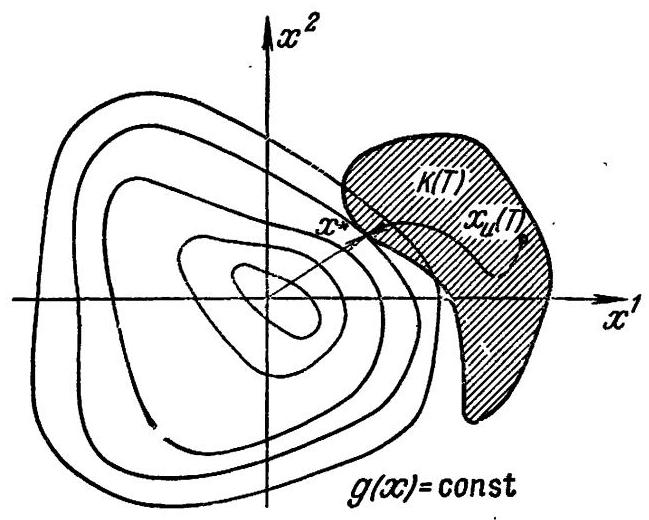
\includegraphics[max width=0.5\textwidth]{images/bo_d547k8bef24c73bgfcg0_539_731_692_649_520_0.jpg}
\end{center}
\hspace*{3em} 

Рис. А2. Наискорейший спуск для нели- нейных управляемых процессов.

Если и принимает значения из гильбертова пространства Ж с нормой \(\left| \cdot \right|  = \langle  \cdot  , \cdot  {\rangle }^{1/2}\) и на \(u\) не наложено никаких ограничений, то можно показать, что градиентное направление наискорейшего спуска в точке и оде Я определяется траекторией, начинающейся в точке и, и удовлетворяющей уравнению

\[
\frac{du}{d\sigma } =  - \frac{\partial g}{\partial x}{\left( {x}_{u}\left( T\right) \right) }^{\prime }h\left( t\right) ,
\]

где \(h\left( t\right)  = {\Phi }_{a}\left( T\right) {\Phi }_{u} - {}^{1}\left( T\right) {B}_{u}\left( t\right)\) , a \({\Phi }_{u}\) есть решение линейного уравнения в вариациях

\[
{\dot{\Phi }}_{u}\left( t\right)  = \frac{\partial f}{\partial x}\left( {{x}_{u}\left( t\right) ,u\left( t\right) }\right) {\Phi }_{u}\left( t\right)
\]

\(\mathrm{c}{\Phi }_{u}\left( {t}_{0}\right)  = I\) и \({B}_{u}\left( t\right)  = \left( {\partial f/\partial u}\right) \left( {{x}_{u}\left( t\right) ,u\left( t\right) }\right)\) на \(\left\lbrack  {{t}_{0},T}\right\rbrack\) .

Чтобы учесть ограничение \(\left| u\right|  \leq  1\) ,положим

\[
\frac{\partial u}{\partial \sigma }\left( {t,\sigma }\right)  =  - \frac{\partial g}{\partial x}{\left( {x}_{u}\left( T\right) \right) }^{\prime }h\left( t\right) ,\;\mathrm{{ec\text{ л }\text{ н }}}\;\left| {u\left( {t,\sigma }\right) }\right|  < 1
\]

Hли если

и

\[
u\left( {t,\sigma }\right) \frac{\partial g}{\partial x}{\left( {x}_{u}\left( T\right) \right) }^{\prime }h\left( t\right)  > 0
\]

\[
\frac{\partial u}{\partial \sigma }\left( {t,\sigma }\right)  = 0,
\]

в противном случае (+, cf), по золу подполагается, чт \(\left| {u\left( {t,0}\right) }\right|  \leq  1\) . Далее видим,что

\[
\frac{dC}{d\sigma } = \frac{\partial g}{\partial \sigma } = \frac{\partial g}{\partial x}{\left( {x}_{u}\left( T\right) \right) }^{\prime }\frac{d{x}_{u}}{d\sigma } =  - {\int }_{J}{\left\lbrack  \frac{\partial {g}^{\prime }}{\partial x}\left( {x}_{u}\left( T\right) \right) h\left( t\right) \right\rbrack  }^{2}{dt} \leq  0,
\]

где \(\mathcal{J} = \left\{  {t \mid  \partial u/\partial \sigma  \neq  0,t \in  \left\lbrack  {{t}_{0},T}\right\rbrack  }\right\}\) . Поэтому есть надежда, что после- довательность приближений, получаемых при решении уравне- ния (†) на вычислительной машине, сходится. В работах Келли (Kelly) и Брайсона (Bryson) содержатся оценки эффективности этого алгоритма.

Пример 6. В этом примере, так же как и в следующем, мы будем применять результаты, полученные в главах 2, 3, 4 и 5, к различным задачам управления. При этом наши сведения об оптимальном управлении будут исчерпывающими лишь в том случае, когда известно начальное значение сопряженного решения. Для того чтобы получить решение, соответствующее этим условиям, мы будем строить функции таким образом, чтобы они достигали своих экстремальных значений при правильных начальных значениях сопряженных решений. Тем самым, задача сведется к рассмотрен- ной в разделе А.1 задаче, где минимум (или максимум) функции, зависящей от конечного числа переменных, отыскивался с помощью метода наискорейшего спуска. Сейчас мы рассмотрим задачу об управлении, оптимальном по быстродействию. Однако результаты можно будет распространить и на задачи с другим критерием ка- чества, а также на нелинейные задачи. (Нейштадт (Neustadt).)

Рассмотрим автономную линейную управляемую систему

\[
\left( \mathcal{L}\right)
\]

\[
\dot{x} = {Ax} + {bu}\left( t\right)
\]

со скалярными управлениями и (t), удовлетворяющими ограниче- нию |u (t)|≤1. Ниже мы будем рассматривать и более общие линейные системы. Пусть задача состоит в приведении системы в начало координат за минимальное время, т. е. совпадает с за- дачей, рассмотренной в главе 2. В главе 2 для этой системы было найдено оптимальное управление, соответствующее любому начальному условию \(\eta \left( {t}_{0}\right)  = c\) ,где \(c -\) постоянняя из некоторого множества. В этом примере мы займемся отысканием этих посто- янных. В задаче оптимального по быстродействию управления, приводящего систему в начало координат, требуется найти на- именышее \(t > 0\) ,для которого уравнение

\[
x\left( t\right)  = {e}^{At}{x}_{0} + {e}^{At}{\int }_{0}^{t}{e}^{-A{t}^{\prime }}{bu}\left( {t}^{\prime }\right) d{t}^{\prime } = 0
\]

удовлетворяется при некотором управлении \(u\left( {t}^{\prime }\right) \left( {0 \leq  {t}^{\prime } \leq  t}\right)\) , удовлетворяющем ограничению \(\left| {u\left( {t}^{\prime }\right) }\right|  \leq  1\) в каждой точке интер- вала [0, t]. Это требование можно записать так:

\[
- {x}_{0} = {\int }_{0}^{t}{e}^{-A{t}^{\prime }}{bu}\left( {t}^{\prime }\right) d{t}^{\prime }
\]

лля некоторого допустимого \(u\left( {t}^{\prime }\right) ,0 \leq  {t}^{\prime } \leq  t\) . Пусть

\[
C\left( t\right)  = \left\{  {x \mid  x = {\int }_{0}^{t}{e}^{-A{t}^{\prime }}{bu}\left( {t}^{\prime }\right) d{t}^{\prime };u\left( {t}^{\prime }\right)  - \text{ допустнмое управление }}\right\}
\]

есть множество начальных состояний, исходя из которых система может достичь начала координат за время, меньшее, чем t. C (t) есть просто особый вид множества достижимости, упоминавшийся в главе 2. На самом деле С (t) = К (—t), с начальной точкой \({x}_{0} = 0\) . Поэтому C (t) является замкнутым, выпуклым множеством в \({R}^{n}\) , c rpаницей

\[
\partial C\left( t\right)  = \left\{  {x\left| {\;x = {\int }_{0}^{t}{e}^{-A{t}^{\prime }}b\operatorname{sgn}\left\{  {c{e}^{-A{t}^{\prime }}b}\right\}  d{t}^{\prime }}\right. ,\parallel c\parallel  = 1}\right\}  .
\]

Более того, если ζ ∈ ∂C (t), а c’ есть внешняя нормаль к C (t) в точке ζ, и если система 8 нормальна, то множество ∂C (t) не содержит никакого отрезка прямой. Заметим, что С (t,) ⊃C (t,), если \({t}_{2} \geq  {t}_{1}\) и \(C\left( t\right)\) непрерывно возрастает с ростом t.

Предположим, что существует некоторое управление, перево- дящее систему из точки х, в точку 0 за конечное время; тогда существует и оптнмальное по быстродействию управление вида

\[
\operatorname{sgn}\{ \eta \left( t\right) b\}  = \operatorname{sgn}\left\{  {c{e}^{-{At}}b}\right\}  ,
\]

переводящее систему из точки х, в 0, где с’есть внешняя нор- маль к множеству \(C\left( {t}^{ * }\right)\) в точке-х,- Обозначим через Z множе- ство всех таких векторов c, где ||c|=1, исходящих из точки \(- {x}_{0} \in  \partial C\left( t\right)\) . Тогда, если \(c \in  Z\) ,то управление

\[
u\left( t\right)  = \operatorname{sgn}\left\{  {c{e}^{-{At}}b}\right\}
\]

переводит систему из состояния \({x}_{0}\) в начало координат и является оптимальным.

Пусть

\[
z\left( {t,c}\right)  = {\int }_{0}^{t}{e}^{-A{t}^{\prime }}b\operatorname{sgn}\left\{  {c{e}^{-A{t}^{\prime }}b}\right\}  d{t}^{\prime }.
\]

Тогда \(z\left( {t,c}\right)  \in  \partial C\left( t\right)\) ,и следовательно, для нормальной системы имеем

\[
{cz}\left( {t,c}\right)  > {c\zeta },\;\zeta  \in  C\left( t\right) ,\;\zeta  \neq  z\left( {t,c}\right) .
\]

3аметим, что

\[
{cz}\left( {t,c}\right)  = {\int }_{0}^{t}c{e}^{-A{t}^{\prime }}b\operatorname{sgn}\left\{  {c{e}^{-A{t}^{\prime }}b}\right\}  d{t}^{\prime } = {\int }_{0}^{t}\left| {c{e}^{-A{t}^{\prime }}b}\right| d{t}^{\prime } > 0\text{ для }t > 0
\]

и, значит, для нормальной системы cz (t, c) есть монотонно воз- растающая функция от t, непрерывная по c.

Рассмотрим (как это делает Нейштадт), функцию

\[
\bar{f}\left( {t,c,{x}_{0}}\right)  = c\left\lbrack  {z\left( {t,c}\right)  + {x}_{0}}\right\rbrack  ,
\]

непрерывную по \(t\) и c. При фиксированных \(\left( {{x}_{0},c}\right)\) она будет строго возрастающей по \(t\) ,так как

\[
\bar{f}\left( {t,c,{x}_{0}}\right)  = {\int }_{0}^{t}\left| {c{e}^{-A{t}^{\prime }}b}\right| d{t}^{\prime } + c{x}_{0}
\]

строго возрастает по t. Рассмотрим теперь лишь те с, для кото- рых \(c{x}_{0} = \bar{f}\left( {0,c,{x}_{0}}\right)  < 0\) . Если с не принадлежит множеству Z, то из условия, что \({cz}\left( {t,c}\right)  > {c\zeta }\) , для всех \(\zeta\) из \(C\left( t\right)\) следует, что \({cz}\left( {{t}^{ * }c}\right)  >  - c{x}_{0}\) или \(\bar{f}\left( {{t}^{ * },C,{x}_{0}}\right)  > 0\) ,где \({t}^{ * } -\) оптимальное время. Следовательно, для некоторого единственного t из интервала \(0 < t < {t}^{ * }\) имеем

\[
\bar{f}\left( {t,c,{x}_{0}}\right)  = 0.
\]

Обозначим это t через \(T\left( {c,{x}_{0}}\right)\) ,так что для каждого с такого, что \(c{x}_{0} < 0\) ,будем иметь \(\bar{f}\left( {T\left( {c,{x}_{0}}\right) ,c,{x}_{0}}\right)  = 0\) .

Поскольку функция f непрерывна по всем аргументам, то и функция \(T\) непрерывна по c. Следовательно, если с ∈Z, то функ- ция T (c, x, принимает свое максимальное значение. Это и есть функция, которую нам придется максимизировать для получения требуемого с.

Для того чтобы найти вектор с, максимизирующий функцию \(T\left( {c,{x}_{0}}\right)\) , paccмотрим векторную функцию \(c\left( \sigma \right)\) ,непрерывно зави- сящую от некоторого параметра о и удовлетворяющую следую- щему дифференциальному уравнению:

\[
\frac{dc}{d\sigma } = k\frac{\partial T}{\partial c},\;\text{ где }{}_{\mathrm{i}}k > 0,
\]

а \(\partial T/\partial c\) есть соответствующий вектор градиента. Для решения этого уравнения применим метод наискорейшего подъема. Для даль- нейшего нам необходимо вычислить вектор

\[
\frac{\partial T}{\partial c} =  - \frac{\partial \overline{f/}\partial c}{\partial \overline{f/}\partial T}.
\]

Из определения \(\bar{f}\left( {T,c,{x}_{0}}\right)\) следует,что

\[
\frac{\partial \bar{f}}{\partial T} = \left| {c{e}^{-{AT}}b}\right|
\]

H

\[
\frac{\partial \bar{f}}{\partial {c}_{i}} = {x}_{0}^{i} + {\int }_{0}^{T}\operatorname{sgn}\left\{  {c{e}^{-A{t}^{\prime }}b}\right\}  {\left\lbrack  {e}^{-A{t}^{\prime }}b\right\rbrack  }^{i}{dt},
\]

где [e \({}^{-{At}}b{\rbrack }^{i}\) есть \(i\) -я компонента вектора е-Агб (для нормальной системы).

Таким образом,

\[
\frac{\partial T}{\partial c} =  - \frac{{\left\lbrack  {x}_{0} + z\left( T,c\right) \right\rbrack  }^{\prime }}{\left| ce - Atb\right| }.
\]

Выбрав \(k = \left| \left\lbrack  {c{e}^{-{At}}b}\right\rbrack  \right|\) ,вычислим новое значение с из уравнения

(††)
\[
\frac{d{c}^{\prime }}{d\sigma } =  - \left\lbrack  {{x}_{0} + z\left( {T\left( {c,{x}_{0}}\right) ,c}\right) }\right\rbrack  .
\]

Поскольку правая часть этого уравнения непрерывна по \(c\) ,то оно имеет решение. Если \(\left| {c{e}^{-{AT}\left( {c,{x}_{0}}\right) }b}\right|  > 0\) , To

\[
\frac{dT}{d\sigma } = \frac{\partial T}{\partial c}\frac{d{c}^{\prime }}{d\sigma } = \left| {c{e}^{-{AT}}\left( {c,{x}_{0}}\right) b}\right| \frac{\partial T}{\partial c}\frac{\partial {T}^{\prime }}{\partial c} \geq  0.
\]

B этом случае, если с ∉Z, то дТ/дс >0. Если |cе-AT (c, x, b) | = 0, то \(\partial T/\partial \sigma\) не определено,но \(\partial \bar{f}/\partial c = {\left\lbrack  {x}_{0} + z\left( T\left( c,{x}_{0}\right) ,c\right) \right\rbrack  }^{\prime }\) опреде- лено для фиксированного \(T\) и \(\left( {\partial \bar{f}/\partial \sigma }\right) \left( {T,c,{x}_{0}}\right)  = \partial \bar{f}/\partial c\partial {c}^{\prime }/\partial \sigma  = \; =  - \partial c/\partial \sigma \partial {c}^{\prime }/\partial \sigma  < 0\mathrm{{при}}c \notin  Z.\mathrm{H}\tau \mathrm{{a\kappa }},\;\phi\) ункция \(\bar{f}\) монотонно убы- вает по σ при фиксированном Т; но, как мы показали ранее, функция f возрастает с ростом \(T\) ; отсюда следует, что если ве- личину \(T\) выразить явно из соотношения \(\bar{f}\) , \(\left( {T,\sigma ,{x}_{0}}\right)  = 0\) как функцию от σ, то получим возрастающую функцию.

Заметим, что значение \(T\left( {c,{x}_{0}}\right)\) определено тогда и только тогда, когда скдео, и если система нормальна, то из соотноше- ния \(c{x}_{0} = 0\) следует, что \(T\left( {c,{x}_{0}}\right)  = 0\) . Пусть D-область опреде- ления функции \(T\left( {c,{x}_{0}}\right)\) . Если вектор \(c\) первоначально находился в \(D\) , то решение с (σ) уравнения (††) остается в D. Для того чтобы вектор \(c\left( \sigma \right)\) вышел за пределы области D, необходимо, чтобы \(c\left( {\sigma }_{0}\right) {x}_{0} = 0\;\Pi\) ри некотором \({\sigma }_{0}\) ,но тогда \(T\left( {c\left( {\sigma }_{0}\right) ,{x}_{0}}\right)  = 0\) . Но это невозможно, так как \(T\left( {c\left( 0\right) ,{x}_{0}}\right)  > 0\) ,и \(T\) возрастает с ростом \(\sigma\) .

Итак, ясно, что функция Т(c, x, o) обращается в нуль на границе дD области D, достигает положительного максимума на выпуклом множестве ZCD, и не имеет в D других локальных максимумов или минимумов. Поэтому, если с (о) стремится к пре- делу при σ →∞, этот предел принадлежит множеству Z. Заме- тим, что \(\parallel c\left( \sigma \right) \parallel  =\) const, noскольку

\[
\frac{d\left( {c{c}^{\prime }}\right) }{d\sigma } = {2c}\frac{d{c}^{\prime }}{d\sigma } =  - {2c}\left\lbrack  {{x}_{0} + z\left( {T,c}\right) }\right\rbrack   = 0.
\]

Для нахождения решения уравнения (††), дающего новое значе- ние с, необходимо применить приближенный метод. Дело в том, что вычисление нулей функции \(\bar{f}\left( {T,c,{x}_{0}}\right)\) ,необходимых для опре- деления \(T\left( {c,{x}_{0}}\right)\) , требует больших затрат машинного времени. Итак, рассмотрим дискретный вариант уравнения (††); пусть

\[
{c}^{\left( j + 1\right) } = {c}^{j} + k\frac{\partial T}{\partial c}\left( {{c}^{\left( j\right) },{x}_{0}}\right) \;{\text{ п }\text{ р }\text{ и }}\;k > 0,
\]

\(i = 1,2,3,\ldots\) ,где функция \(T\left( {{c}^{\left( j\right) },{x}_{0}}\right)\) ompeдeляется следующим образом: увеличиваем t до тех пор, пока выражение f \(\left( {t,{c}^{\left( j\right) },{x}_{0}}\right)  = \; = {c}^{\left( j\right) }\left\lbrack  {{x}_{0} + z\left( {t,{c}^{\left( j\right) }}\right) }\right\rbrack\) не обратится в нуль, и берем в качестве T \(\left( {{c}^{\left( j\right) },{x}_{0}}\right)\) соответствующее значение t. Для этого приходится прибегать лишь к интег- рированию, которое вычислительная машина производит довольно быстро [см. Паевонский (Paiewonsky)]. После того как найдено \(T\left( {{c}^{\left( j\right) },{x}_{0}}\right) ,{c}^{\left( j + 1\right) }\) вы- числяется из указанного рекуррент- ного соотношения. Затем вся проце- дура повторяется для вычисления \(T\left( {{c}^{j + 1},{x}_{0}}\right) ,u\) Так далее. Скорость сходимости этого процесса определяет- ся выбором постоянной \(k > 0\) .

\begin{center}
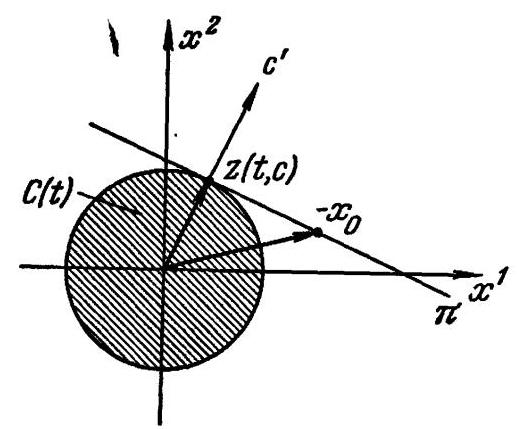
\includegraphics[max width=0.4\textwidth]{images/bo_d547k8bef24c73bgfcg0_544_246_1030_517_429_0.jpg}
\end{center}
\hspace*{3em} 

Рис. А3. Построение наискорейшего спуска для управлений, оптималь- ных по быстродействию.

Этот метод имеет простую геометрическую интерпретацию. Пусть (рис. А3) — хо-произвольная точка, а с —любой нулевой вектор, такой, что скде о. Увеличению и до тех пор, пока не насту- пит равенство \(f\left( {t,c,{x}_{0}}\right)  = c\left\lbrack  {{x}_{0} + z\left( {t,c}\right) }\right\rbrack   = 0\) , cootветствует па- раллельное перемещение гиперплоскости π: с [—х+ z(t, c)]=0 до тех пор, пока она не пройдет через точку — \({x}_{0}\) . При этом вектор \(c\) меняется так, чтобы вектор — \({x}_{0} - z\left( {t,c}\right)  = v\) стал ортогональ- ным вектору \({c}^{\prime }\) . Далее проводится итерация, как показано выше.

Обобщим теперь наши результаты для случая системы с пе- ременными коэффициентами и m управляющими переменными. Рассмотрим систему

\[
\text{ (C) }\dot{x} = A\left( t\right) x + B\left( t\right) u\left( t\right)  + v\left( t\right) ,\left| {{u}^{j}\left( t\right) }\right|  \leq  1,j = 1,2,\ldots ,m\text{ , }
\]

где \(A\left( t\right) ,B\left( t\right)  -\) как обычно, maтрицы,непрерывные по \(t\) , paзме- ров n×n и n×m соответственно, а v(t)—заданная непрерывная вектор-функция, определенная на рассматриваемом интервале.

Решение этого линейного уравнения, соответствующее некото- рому измеримому управлению и (t), имеет вид

\[
x\left( t\right)  = \Phi \left( t\right) {x}_{0} + {\int }_{{t}_{0}}^{t}\Phi \left( t\right) {\Phi }^{-1}\left( {t}^{\prime }\right) \left\lbrack  {B\left( {t}^{\prime }\right) u\left( {t}^{\prime }\right)  + v\left( {t}^{\prime }\right) }\right\rbrack  d{t}^{\prime },
\]

где

\[
\dot{\Phi }\left( t\right)  = A\left( t\right) \Phi \left( t\right) \;\text{ и }\;\Phi \left( {t}_{0}\right)  = I.
\]

Переписывая указанное выше уравнение, получнм

\[
- {x}_{0} - {\int }_{{t}_{0}}^{t}{\Phi }^{-1}\left( {t}^{\prime }\right) v\left( {t}^{\prime }\right) d{t}^{\prime } + {\Phi }^{-1}\left( t\right) x\left( t\right)  = {\int }_{{t}_{0}}^{t}{\Phi }^{-1}\left( {t}^{\prime }\right) B\left( {t}^{\prime }\right) u\left( {t}^{\prime }\right) d{t}^{\prime }.
\]

Предположим, что задача состоит в определении такого до- пустимого управления, которое обеспечивало бы достижение ра- венства x(t)=ξ(t) за минимальное время, где ξ(t)—параметри- ческое представление некоторой непрерывной кривой в R".

Пусть

\[
\omega \left( t\right)  =  - \left\lbrack  {{x}_{0} + {\int }_{{t}_{0}}^{t}{\Phi }^{-1}\left( {t}^{\prime }\right) v\left( {t}^{\prime }\right) d{t}^{\prime } - {\Phi }^{-1}\left( t\right) \xi \left( t\right) }\right\rbrack  .
\]

Тогда для осуществления оптимального по быстродействию управ- ления системой необходимо найти такое допустимое управление \(u\left( t\right)\) и время t, для которых

\[
\omega \left( t\right)  = {\int }_{{t}_{0}}^{t}{\Phi }^{-1}\left( {t}^{\prime }\right) B\left( {t}^{\prime }\right) u\left( {t}^{\prime }\right) d{t}^{\prime }
\]

с минимальным \({t}_{1}\) Поскольку о (не съ точка пространства \({R}^{n}\) для каждого \(t\) , то можно рассмотреть такое же множество \(C\left( t\right)\) , как и раньше, и задача сводится к нахождению наименьшего t, для которого ω(t) ∈ C (t). Рассмотрим снова максимизирующие управления

\[
{u}^{j}\left( t\right)  = \operatorname{sgn}{\left\{  c{\Phi }^{-1}\left( t\right) B\left( t\right) \right\}  }_{j},\;j = 1,2,\ldots ,m,
\]

ми предположим, что ни одна из компонент вектора \{cD"1 (d) B(t)\} не обращается в нуль на некотором интервале при \(\parallel c\parallel  = 1\) ,т. е., что система нормальна.

Пусть, как обычно

\[
z\left( {t,c}\right)  = {\int }_{{t}_{0}}^{t}{\Phi }^{-1}\left( {t}^{\prime }\right) B\left( {t}^{\prime }\right) \operatorname{sgn}\left\{  {c{\Phi }^{-1}\left( {t}^{\prime }\right) B\left( {t}^{\prime }\right) }\right\}  d{t}^{\prime },
\]

где \(z\left( {t,c}\right)\) принимает значения из множества дО( t), a c’-внешняя нормаль к множеству \(C\left( t\right)\) в точке \(z\left( {t,c}\right)\) . Рассмотрим соотноше- ние \(\bar{f}\left( {t,c,\omega \left( t\right) }\right)  = c\left\lbrack  {z\left( {t,c}\right)  - \omega \left( t\right) }\right\rbrack\) . Геометрическая интерпрета- ция этой задачи приведена на рис. А4, (для дискретных значе- ний с). В качестве первого приближения выберем любой вектор \({c}^{\left( 1\right) }\) , \(\mathrm{y}\) довлетворяющий условиям \({c}^{\left( 1\right) }\omega \left( {t}_{0}\right)  > 0,\left\lVert \begin{array}{c} {c}^{\left( 1\right) } \end{array} \right\rVert = 1\) . Далее будем увеличивать \(t\) до тех пор, пока функция \(f\left( {t,{c}^{\left( 1\right) },\omega \left( t\right) }\right)\) не станет равной 0, что соответствует параллельному движению гиперплос- кости я до тех пор, пока она не пересечет кривой ω (t). Пусть это произойдет в момент \(t = {t}^{\left( 1\right) }\) . Если \(\omega \left( {t}^{\left( 1\right) }\right)  \neq  z\left( {{t}^{\left( 1\right) },{c}^{\left( 1\right) }}\right)\) ,то нужно сделать следующий шаг. Для этого выберем вектор \({c}^{\left( 2\right) } = {c}^{\left( 1\right) } + k{v}^{\left( 1\right) }\) ,где \({v}^{\left( 1\right) }\) -век- тор, соединяющий конец вектора \(z\left( {{t}^{1},{c}^{1}}\right)\) с точкой \(\omega \left( {t}^{\left( 1\right) }\right)\) . Таким обра- 30M, получим

\[
{c}^{\left( 2\right) } = {c}^{\left( 1\right) } + k\left\lbrack  {\omega \left( {t}^{\left( 1\right) }\right)  - z\left( {{t}^{\left( 1\right) },{c}^{\left( 1\right) }}\right) }\right\rbrack  ,
\]

\begin{center}
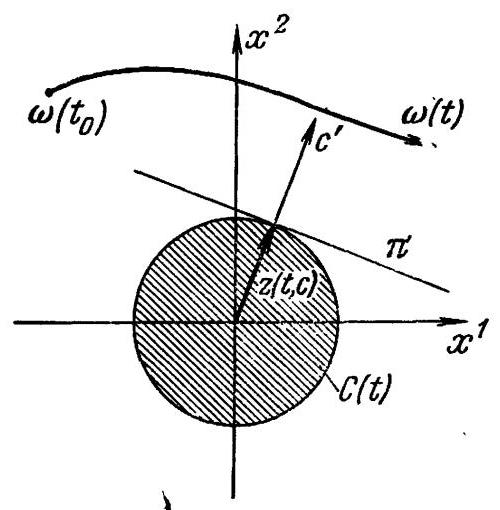
\includegraphics[max width=0.4\textwidth]{images/bo_d547k8bef24c73bgfcg0_546_178_568_500_510_0.jpg}
\end{center}
\hspace*{3em} 

Pac. A4. \({}^{\prime }\) Hanckopeämult cnyck в случае зависящего от времени це- левого множества.

где \(k > 0\) . Опять легко показать, что v есть направление градиента к T, где \(T\left( {T > {t}_{0}}\right)\) есть наименьший корень уравнения \(\bar{f}\left( {t,c,\omega \left( t\right) }\right)  = 0\) .

Если оптимальное управление существует, и если к выбрано правильно, то итеративный процесс приведет к некоторому век- тору \(c \in  Z\) , который мы обозначим через \({c}^{ * }\) . Тогда оптимальное управление, переводящее систему в точку кривой ω (t), будет равно

\[
u\left( t\right)  = \operatorname{sgn}\left\lbrack  {{c}^{ * }{\Phi }^{-1}\left( t\right) B\left( t\right) }\right\rbrack  .
\]

Реализация этого алгоритма на аналоговой и цифровой вычисли- тельных машинах имеется в работе Паевонского (Paiewonsky). Он также применил некоторые методы, разработанные Н. Н. Красов- ским и непосредственно связанные с рассмотренными выше пост- роениями.

Пример 7. Рассмотрим управляемую систему

(5)
\[
\dot{x} = f\left( {x,u}\right) ,\;x\left( {t}_{0}\right)  = {x}_{0},\;u \in  \Omega
\]

скритерием качества

\[
C\left( u\right)  = g\left( {x\left( T\right) }\right) ,
\]

где T —фиксированное время окончания процесса управления. Предполагается, что \(f \in  {C}^{1}\) в \({R}^{n} \times  \Omega\) и \(g \in  {C}^{1}\) в \({R}^{n}\) . C помощью принципа максимума (см. главы 1 и 5) часто бывает возможно получить управление и как функцию состояния х и сопряженной переменной \(\eta\) , maxсимизируя выражение \(H = \eta \dot{x} = {\eta f}\left( {x,u}\right)\) по \(u\) , явно входящему в H для \(u \in  \Omega\) . Мы будем рассматривать лишь те задачи, в которых гакое единственное управление и существует. В этом случае задача сводится к нахождению такого начального вектора \(\eta \left( {t}_{0}\right)\) ,чтобы экстремальная кривая удовлетворяла зáдан- ным граничным условиям и минимизировала бы функционал

\[
C\left( u\right)  = g\left( {x\left( T\right) }\right) .
\]

Будем рассматривать только максимальные кривые, т. е. ре- шение дифференциальных уравнений

\[
\left( {\mathcal{S}}_{E}\right)
\]

\[
\dot{x} = \frac{\partial H\left( {x,\eta ,U}\right) }{\partial \eta } = f\left( {x,U\left( {x,\eta }\right) }\right)  = \widetilde{f}\left( {x,\eta }\right) ,
\]

\[
\dot{{\eta }^{\prime }} =  - \frac{\partial H\left( {x,\eta ,U}\right) }{\partial x} =  - \frac{\partial f}{\partial x}\left( {x,U\left( {x,\eta }\right) }\right) {\eta }^{\prime } = {\widetilde{g}}^{\prime }\left( {x,\eta }\right) ,
\]

где \(U = U\left( {x,\eta }\right)\) определяется из условия

\[
H\left( {x,\eta ,U}\right)  = \mathop{\max }\limits_{{u \in  \Omega }}\{ H\left( {x,\eta ,u}\right) \} \text{ для всех }x,\eta  \in  {R}^{n}.
\]

Здесь \(x\left( {t}_{0}\right)  = {x}_{0}\) и η( \({t}_{0}\) ) требуется определить так, чтобы удовле- творялись заданные граничные условия (см. ниже), и чтобы дости- гался минимум g (x (T)).

Итак, наша задача сведена к исследованию семейства кривых, зависящих от \(n\) параметров \(\eta \left( {t}_{0}\right)\) . Цель наших вычислений — опре- делить вектор \(\eta \left( {t}_{0}\right)\) так, чтобы соответствующее решение системы \({\mathcal{S}}_{E}\) минимизировало бы функцию \(g\) .

Для каждого \(\eta \left( {t}_{0}\right)  = c\) решение системы \$ запишем в виде

\[
\left\lbrack  \begin{array}{l} x\left( {t,c}\right) \\  {\eta }^{\prime }\left( {t,c}\right)  \end{array}\right\rbrack
\]

причем предполагается, что по заданному и = U (x, η) всегда можно вычислить такое решение. В этом случае нетрудно определить и \(g\left( {x\left( {T,c}\right) }\right)\) . Мы ищем такую функцию \(c\left( \sigma \right)\) ,чтобы функционал \(g\left( {x\left( {T,c\left( \sigma \right) }\right) }\right)\) , paccматриваемый как функция от σ, убывал с возра- станием σ.

Пусть зависимость с от σ определена из уравнения наискорей- шего спуска

(
\[
\forall \forall
\]
 )
\[
\frac{dc}{d\sigma } =  - k\frac{\partial g}{\partial c},
\]

где \({\left\lbrack  \partial g/\partial c\right\rbrack  }^{\prime }\) -вектор градиента,а \(k =\) const \(> 0\) . Тогда

\[
\frac{dg}{d\sigma } = \frac{\partial g}{\partial c}\frac{\partial {c}^{\prime }}{\partial \sigma } =  - k{\left\lbrack  \frac{\partial g}{\partial c}\right\rbrack  }^{2} \leq  0,
\]

где под [др/о)2 понимается скалярное произведение. Если дд/дс ≠ 0, то функция \(g\left( \sigma \right)  = g\left( {x\left( {T,c\left( \sigma \right) }\right) }\right)\) yóывает с возрастанием σ, a зна- чит,точка,где \(\partial g/\partial c = 0\) ,достигается при \(\sigma  \rightarrow  \infty\) .

Чтобы вычислить с(σ) из указанного выше уравнения (†††), необходимо знать, как меняется g в зависимости от с. Поэтому рассмотрим уравнение

\[
\frac{\partial g}{\partial c} = \frac{\partial {g}^{\prime }}{\partial x}\frac{\partial x}{\partial c},
\]

гле \(x = x\left( {T,c}\right)\) ,и

\[
\frac{\partial x}{\partial {c}^{\prime }} = \left[ \begin{array}{ccc} \frac{\partial {x}^{1}}{\partial {c}_{1}} & \cdots & \frac{\partial {x}^{1}}{\partial {c}_{n}} \\  \vdots & & \\  \frac{\partial {x}^{n}}{\partial {c}_{1}} & \cdots & \frac{\partial {x}^{n}}{\partial {c}_{n}} \end{array} \right]  .
\]

Для того чтобы вычислить эту матрицу, требуется выяснить, как сильно меняются решения при малом изменении с. Поскольку

\[
\dot{x} = \widetilde{f}\left( {x,\eta }\right) ,\;\dot{\eta } = \widetilde{g}\left( {x,\eta }\right) ,
\]

то максимальное решение (x(t, c), η(t, c)) должно удовлетворять системе уравнений

\[
\dot{x}\left( {t,c}\right)  = \widetilde{f}\left( {x\left( {t,c}\right) ,\eta \left( {t,c}\right) }\right) ,\;\dot{\eta }\left( {t,c}\right)  = \widetilde{g}\left( {x\left( {t,c}\right) ,\eta \left( {t,c}\right) }\right)
\]

при \({t}_{0} \leq  t \leq  T\) . Pacсмотрнм снстему уравнений

\[
\frac{\partial \dot{x}\left( {t,c}\right) }{\partial {c}_{i}} = \frac{\partial \widetilde{f}}{\partial x}\left( {x\left( {t,c}\right) ,\eta \left( {t,c}\right) }\right) \frac{\partial x}{\partial {c}_{i}}\left( {t,c}\right)  + \frac{\partial {\widetilde{f}}^{\prime }}{\partial \eta }\left( {x\left( {t,c}\right) ,\eta \left( {t,c}\right) }\right) \frac{\partial {\eta }^{\prime }}{\partial c}\left( {t,c}\right) ,
\]

\[
\frac{\partial {\widetilde{\eta }}^{\prime }\left( {t,c}\right) }{\partial {c}_{i}} = \frac{\partial {\widetilde{g}}^{\prime }}{\partial x}\left( {x\left( {t,c}\right) ,\eta \left( {t,c}\right) }\right) \frac{\partial x}{\partial {c}_{i}}\left( {t,c}\right)  + \frac{\partial \widetilde{g}}{\partial \eta }\left( {x\left( {T,c}\right) ,\eta \left( {t,c}\right) }\right) \frac{\partial {\eta }^{\prime }}{\partial {c}_{i}}\left( {t,c}\right) .
\]

В предположении, что изменение порядка дифференцирования в данном случае допустимо, получаем

\[
\frac{d\left( \frac{\partial x}{\partial {c}_{i}}\right) }{dt} = \frac{\partial \widetilde{f}}{\partial x}\frac{\partial x}{\partial {c}_{i}} + \frac{\partial {\widetilde{f}}^{\prime }}{\partial \eta }\frac{\partial {\eta }^{\prime }}{\partial {c}_{i}},
\]

(F)
\[
\frac{d\left( \frac{\partial {\eta }^{\prime }}{\partial {c}_{i}}\right) }{dt} = \frac{\partial {\widetilde{g}}^{\prime }}{\partial x}\frac{\partial x}{\partial {c}_{i}} + \frac{\partial \widetilde{g}}{\partial \eta }\frac{\partial \widetilde{\eta }}{\partial {c}_{i}},
\]

где производные д \(\widetilde{f}/\partial x,\partial \widetilde{f}/\partial \eta ,\partial \widetilde{g}/\partial x,\partial \widetilde{g}/\partial \eta\) вычисляютея вдоль эк- стремальной кривой \(x\left( {t,c}\right) ,\eta \left( {t,c}\right) \left( {{t}_{0} \leq  t \leq  T}\right)\) . Пусть

\[
\psi \left( t\right)  = \left\lbrack  \begin{array}{ll} {\psi }_{1}^{1}\left( t\right) & {\psi }_{2}^{1}\left( t\right) \\  {\psi }_{1}^{2}\left( t\right) & {\psi }_{2}^{2}\left( t\right)  \end{array}\right\rbrack
\]

— фундаментальная матрица решений системы линейных уравне- ний \(\overline{\mathcal{L}}\) , удовлетворяющая начальному условию ψ( \({t}_{0}\) ) = 1 . Тогда

\[
\frac{\partial g}{\partial t} = \frac{\partial {g}^{\prime }}{\partial x}{\psi }_{2}^{1}\left( T\right) ,
\]

где функция \({\psi }_{2}^{1}\left( T\right)\) зависит, конечно, от максимальной кривой \(x\left( {t,c}\right) ,\eta \left( {t,c}\right)\) ,так что с возрастанием σ величина \({\psi }_{2}^{1}\left( T\right)\) непре- рывно меняется. Таким образом, локальная чувствительность ре- шений может быть оценена с помощью вариационного подхода.

Другой метод, часто употребляемый при машинных вычисле- ниях, состоит в приближенном вычислении дg/дс с помощью ме- тода возмущений [см., например, Шармак (Scharmack)].

Существуют различные применения вычислительного алгоритма, основанного на методе наискорейшего спуска, к задачам простран- ственной навигации (Шармак) и к некоторым другим задачам [Kenли-Брайсон (Kelley-Bryson)].

\section*{А.3. Работы по методу наискорейшего спуска и вычислительным методам оптимального управления}

В двух предыдущих разделах метод наискорейшего спуска был предложен в качестве конструктивного метода построения опти- мальных управлений. Многие из алгоритмов для вычисления оп- тимальных управлений основаны на методе наискорейшего спуска; точнее говоря, почти все из них, даже методы, рассмотренные в примерах 5 и 6, основаны на некоторых модификациях метода наискорейшего спуска. В примере 5, например, модификация со- стоит в изменении отсчета времени с помощью постоянной k. В дальнейших модификациях меняется уже геометрия функцио- нального пространства [в методе Ньютона—Рафсона (Newton — Raphson) для систем второго порядка вводится локально-линейное преобразование]. При рассмотрении различных специальных клас- сов задач применяются и другие модификации, позволяющие уве- личить эффективность алгоритма; кроме того, существуют и такие методы вычисления оптимальных управлений, как метод динами- ческого программирования [Беллман (Bellman)] и другие, кото- рые не имеют никакого отношения к методу наискорейшего спуска. Общая теория метода наискорейшего спуска излагается в статьях Голдстейна (Goldstein), Канторовича и Розенблюма (Rosenbloom).

В литературе встречается множество прекрасных примеров применения метода наискорейшего спуска к задачам оптимального управления. В частности, несколько примеров есть в статьях Брайсона и Келли. Поскольку авторы настоящей книги сами до- статочно серьезно не занимались применением метода наискорей- шего спуска, то мы не будем здесь высказывать своего мнения о преимуществах одного вычислительного метода перед другим. Мы завершаем этот раздел подробной библиографией по методу наискорейшего спуска и другим численным методам. Мы, однако, расположили работы по разделам, указывая, как нам кажется, сферу применения результатов каждой из работ.

\section*{библиогрАфия к приложению А}

\section*{Метод наискорейшего спуска и оптимизация управлений}

Balakrishnan A. V., An Operator Theoretic Formulation of a Class of Control Problems and a Steepest Descent Method of Solution. J. Soc. Ind. Appl. Math., Ser. A, Control, 1, No. 2, 109-127 (1963).

Curry H. B., The Method of Steepest Descent for Nonlinear Minimization Problems. Quart. Appl. Math., 2, № 4 (Oct. 1944).

D en h a m W. F., Steepest-Ascent Solution of Optimal Programming Problems. Ph. D. Thesis, Div. Engr. and Applied Physics, Harvard University (1963).

Goldstein A. A., Minimizing Functionals on Hilbert space, In A. V. Ba-lakrishnan and L. W. Neustadt (eds.). Computing methods in Optimization Problems, Academic Press Inc., New York, 1964, pp. 159-165. [CM. также J. Soc. Ind. Appl. Math. Ser. A, Control 4, 81-89 (1966).]

Gollwitzer H. E., Application of the Method of Steepest Descent to Optimal Control Problems. Thesis, University of Minnesota. 1965.

H i 11 sl e y R. H., R o b i n s H. M., Steepest Ascent Trajectory Optimization Method Which Reduces Memory Requirements. B книге: A. V. Balakrishnan, L. W. Neustadt (eds.), Computing Methods in Optimization Problems, Academic Press Inc., New York, 1964, pp. 107-133.

Канторович Л. В., Акилов Г. П., Функциональный анализ в нор- мированных пространствах, Физматгиз, 1959.

Rosenbloom P. C., The Method of Steepest Descent. Proceedings of Symposia in Applied Mathematics, vol. 6, pp. 127-176, The American Mathematical Society, 1956.

Tompkins C. B., Method of Steepest Descent. B к н а re: F. F. B e c ken-b a c h (ed.) Modern Mathematics for the Engineer. McGraw-Hill Book Co., Inc., New York, 1956, Chapter 18.

V a ch i n o R. F., Steepest Descent with Inequality Constraints on the Control Variables, J. Soc. Ind. Appl. Math., Ser. A, Control 4, No 1, 245-261 (1966).

В айнберг М. М., О сходимости метода наискорейшего спуска для нели- нейных уравнений. ДАН СССР, т. 130, № 1, 1960.

Метод наискорейшего спуска в применении к проблемам оптимизации управлений

Bryson A. E. Denham W. F., A Steepest Ascent Method for Solving Optimum Programming Problems. J. Appl. Mech. 29, 247-257 (1962).

Bryson A. E., Denham W. F., Caroll E. J., Mikamic K., Determination of the Lift or Drag Program that Minimizes Re-entry Heating with Acceleration or Range Constraints Using a Steepest Descent Computation Procedure. J. of Aerospace Sci., 29, № 4, 420-430 (1962).

Denham W. F., Bryson A. E., Optimal programming with inequality constraints, II: Solution by steepest ascent. AIAAJ 2, 25-34 (1964).

Neust a dt L. W., Minimum Effort Control Systems. J. Soc. Ind. Appl. Math., Ser. A., Control 1, № 1, 16-31 (1962).

N eust at L. W., Synthesizing Time Optimal Control Systems. J. Math. Anal. Appl., 1, № 4, 484-493 (1960).

\section*{Численные методы в задачах оптимизации управлений}

A o k i M., On a Successive Approximation Technique in Solving Some Control Problems. Trans. ASME, Ser. D. J. Basic Eng. 85, 177-180 (1963).

Balakrishn'an A. V., Hsieh H. C., Function Space Methods in Control System Optimization. Proc. Optimum System Synthesis Conference, Dayton, Ohio, September 1962, pp. 10-40.

Bohn E. V., A Numerical Trajectory Optimization Method Suitable for a Computer of Limited Memory. Proc. JACC Seattle, Washington, 1966, 177-186.

Breakwell J. V., Speyer J. L., Bryson A. E., Optimization and Control of Nonlinear Systems Using Second Variation. J. Soc. Ind. appl. Math., Ser. A, Control, 1, № 2, 193-223 (1963).

Canon M. D., Eaton J. H., A New Algorithm for a Class of Quadratic Programming Problems with Applications to Control. J. Soc. Ind. Appl. Math., Ser. A, Control, 4, № 1, 34-45 (1966).

E at on J. H., An Interative Solution to Time-Optimal Control. J. Math. Anal. Appl., 5, 324-344 (1962).

E a to n J. H., An On Line Solution to Sampled-Data Time Optimal Control. J. Electron. Control, 15, № 4, 333-341 (1963).

E a ton J. H., Improper Solutions under Existence Assumptions: an Example. Tech. Note on NASA Grant NsG-354, Ser. 5, Issue 16, University of California (1964).

F a dden E. J., Gilbert E. G., Computational Aspects of the Time-Optimal Control Problem. B книге: A. V. Balakrishnan, L. W. Ne-u s t a d t (peд.), Computing Methods in Optimization Problems. Academic Press Inc., New York, 1964, pp. 167-193.

F an cher P. S., Iterative Computation Procedures for an Optimum Control Problem. IEEE Trans. Auto., Control AC-10, 346-348 (1965).

F letcher R., P ow ell M. J. D., A Rapidly Convergent Descent Method for Minimization. Computer Journal, 6, № 2, 163-168 (1963).

Fletcher R., Reeves C. M., Function Minimization by Conjugate Gradients. Computer Journal, 7, № 2, 149-154 (1964).

Forsy the G. E., Acceleration of the Optimum Gradient Method, Abstract. Bull. Amer. Math. Soc., 57, 304-305 (1951).

For sythe G. E., M o t z k in T. S., Asymptotic Properties of the Optimum Gradient Method (Abstract), Bull. Amer. Math. Soc. 57, 183 (1951).

Frank M., Wolfe P., An Algorithm for Quadratic Programming, Naval Res. Logist, Quart., 3, 95-110 (1956).

Gilbert E. G., An Iterative Procedure for Computing the Minimum of a Quadratic Form on a Convex Set. J. Soc. Ind. Appl. Math. Ser. A, Control, 4, № 1, 61-80 (1966).

G ottilieb R. G., Rapid Convergence to Optimum Solutions using Min-H Strategy. Proc. JACC, Seattle, Washington, 1966, pp. 167-174.

Gold stein A. A., Convex Programming and Optimal Control, J. Soc. Ind. Appl. Math., Ser. A, Control, 3, Ne 1, Ser. A., 147-151 (1965).

Halkin H., Method of convex ascent. B книге: A. V. Balakrishnan, L. W. Neus t a dt (eds.), Computing Methods in Optimization Problems, Academic Press Inc., New York, 1964, pp. 211-239.

H o Y. C., A Successive Approximation Technique for Optimal Control Systems Subject to Input Saturation. Trans. ASME, Ser. D. J. Basic Eng., 84, № 1, 33-40 (1962).

H o Y. C., Computational Procedure for Optimal Control Problem with State Variable Constraints, J. Math. Anal. Appl. 5, 216-224 (1962).

Но Y. C., Brentani P. B., On Computing Optimal Control with Inequality Constraints, J. Soc. Ind. Appl. Math., Ser. A, Control, 319-348 (1963).

Но Y. C., Kash y a p R. L., A Class of Iterative Procedures for Linear Inequalities, J. Soc. Ind. Appl. Math. Ser. A, Control 4, No 1, 112-115 (1966).

Isaacs D., Leondes C. T., Nieman R. A., On a Sequential Optimization Approach in Nonlinear Control. Proc. JACC, Seattle, Washington, 158-166, 1966.

Jurovics A. S., McIntyre J. E., The Adjoint Method and its Application to Trajectory Optimization, ARS J., 32, 135s (1962).

K a z d a L., Control System Optimization Using Computers as Control System Elements, Proc. of Computer in Control Systems Conference, New York, 1958.

Kelley H. J., Methods of Gradients. B книге: G. Leitman (ed.) Optimization Tecdniques, Academic Press Inc., New York, 1962, Chapter 6.

Knapp C. H., Frost P. A., Determination of Optimal Control and Trajectories Using the Maximum Principle in Association with a Gradient Technique. Proc. JACC, Stanford, California, 1964, p. 222.

K n u d s e n H. K., An Iterative Procedure for Computing Time-Optimal Controls, IEEE Trans. Auto. Control, 9, 23-30 (1964).

K opp R. E., Mc Gill R., Several Trajectory Optimization Techniques. B книге: A. V. Balakrishnan and L. W. Neusta dt. (ed.) Computing Methods in Optimization Problems. Academic Press Inc., New York, 1964, pp-65-89.

K uliko wski R., Synthesis of a Class of Optimum Control Systems. Bull. Acad. Polon. Sci., Ser. Sci., Tech. 7, 663-671 (1959).

L uh J. Y. S., On a Computational Scheme for Time Optimal of Linear Discrete Systems, IEEE Trans. Auto. Control, ACll, No 1, 145 (1966).

McGill R., Optimal Control, Inequality State Constraints, and the Generalized Newton-Raphson Algorithm. J. Soc. Ind. Appl. Math., Ser. A, Control 3, № 2, 291-298 (1965).

McReynolds S. R., A Successive Sweep Method for Solving Optimal Programming Problems, Ph. D. Dissertation, Div. of Engineering and Appl. Physics, Harvard University (1966).

M e e p o h B., Φ p и д ма h B. Г., Линейное программирование в гиль- бертовом пространстве и оптимизация одного класса многосвязных систем. Труды III Конгресса ИФАК, Лондон, 1966.

Merriam C. W., An Algorithm for the Iterative Solution of a Class of Two Point Boundary Value Problems, SIAM J., Control, 2, 1-10 (1964).

Mika mi T., An Iterative Computing Method for Solving Time-Optimal Problems. Proc. Third IFAC Congress, London (1966).

Mitter S. K., Successive Approximation Methods for the Solution of Optimal Control Problems. Automatica 3, 135-149, Pergamon Press (1966).

M over H. G., Purham G., Several trajectory optimization techniques, Part II. B книге: A. V. Balakrishnan and L. W. Neustadt (ed.), Computing Methods in Optimization Problems. Academic Press Inc., New York (1964), pp. 91-105.

Neustadt L. W., A Synthesis Method for Optimal Controls. Proc. of Optimum System Synthesis Conference, Dayton, Ohio (September 1962), pp. 273-382.

No to n A. R., Numerical computation of automatic control, Proc. JACC, Seattle, Washington (1966), pp. 193-204.

Paiewonsky B., Woodrow P., Brunner W., Halbert P., Synthesis of Optimal Controllers Using Hybrid Analog-digital Computers. B книге: A. V. B alakrishnan and L. W. Neustadt (eds.), Computing Methods in Optimization Problems. Academic Press Inc., New York (1964). pp. 285-304.

Plant J. B., A than s M., An iterative Technique for the Computation of Time Optimal Controls. Proc. Third JFAC Congress, London (1966).

Rosen J. B., Iterative Solution of Nonlinear Optimal Control Problems. J. Soc. Ind. Appl. Math., Ser. A, Control, 4, Ne I, 223-244 (1966).

Rosen J. B., Optimal Control and Convex Programming. B книге: J. A b a d i e (ed.), Nonlinear Programming, A Course, North-Holland Publishing Company, Amsterdam (1966).

Sch arm ack D. K., The Equivalent Minimization Problem and the Newton-Raphson Optimization Method. Proc. of the Optimum System Synthesis Conference, Dayton, Ohio (September 1962), pp. 119-158.

Scheley C. H., Optimal Control Computation by the Newton-Raphson Method and the Riccati Transformation. Proc. JACC, Seattle, Washington (1966), pp. 186–192.

Shah B. V., Buehier R. J., Kempthrone O., Some Algorithms for Minimizing a Function of Several Variables. J. Soc. Ind. Appl. Math., 12, 74 (1964).

\section*{Применение вычислительной техники к прикладным задачам теории управления}

B att in R. H., A Statistical Optimizating Navigation Procedure for Space Flight, ARS J., 1681-1698 (1962).

Bellman R., Dreyfus S., An application of Dynamic Programming to the Determination of Optimal Safellite Trajectories, J. Brit. Interplanet. Soc. № 3-4, 17, 78-83 (May-August 1958).

K elley H. J. Successive Approximation Techniques for Trajectory Optimization, Proc. of the IAS Symposium on Vehicles System Optimization, Institute of Aerospace Sciences, New York (1961), p. 10.

L and graf S. K., Some Practical Application of Performance Optimization Techniques to High-Performance Aircraft. J. Aircraft, 2, № 2, 153-154 (1965).

Meditch J., Optimal Thrust Programming for Minimal Fuel Midcourse Guidance, Proc. of Optimum Synthesis Conference, Dayton, Ohio (1962), pp. 55-68.

Melbourn e W. G., Sauer C. G. Constant Attitude Thrust Program Optimization, AIAAJ, 3, 8, 1428-1431 (1965).

Melbourn e W. G., S auer C. G., Optimum Thrust Program for Power Limited Propulsion Systems, Astronaut., Acta 8, 1962.

P ai e won s'k y B. H., The Syntheis of Optimal Controller. Proc. of the Optimum System Synthesis Conference, Dayton, Ohio, (September 1962), pp. 69-88.

Smith F. T., Optimization of Multistage Orbit Transfer Processes by Dynamic Programming. ARS J. 31, pp. 1553—1559 (1961).

Spang H. A., III, Optimum Control of an Unknown Linear Plant Using Bayesian Estimation of the Error. IEEE Trans., Control AC-10, № 1, 80-83 (1965).

S wer ling P., A Proposed Stagewise Differential Condition Procedure for Satellite Tracking and Prediction, J. Astro. Sci., 6, 46-52 (1959).

T s i e n H. S., E v a n s R. C., Optimum Thrust Programming for Sounding Rocket. ARS J., 21, 99-107 (1951).

\section*{Обзорные статьи, посвященные оптимизации управлений с применением вычислительной техники}

Bell D. J., A Review of Flight Path Optimization ... in the Period 1945-1960, J. Roy. Aeron. Soc. 67, 119 (1963).

Greenley R. R., Comments on the Adjoint Method and its Application to Trajectory Optimization, AIAA J., 1, 1463 (1963).

Paiewonsky B. H., A Study of Time Optimal Control. B книге: J. P. L a s a 11e, S. L e f s h e t z (ed.), Proceedings of International Symposium on Nonlinear Differential Equations and Nonlinear Mechanics, Academic Press Inc., New York (1963), pp. 333-365.

P aiewonsk y B. H., Optimal Control: A Review of Theory and Practice AIAA J. 3, 11, 1985—2006 (1965).

S p a n g H. A., III, A Review of Minimization Techniques for Nonlinear Functions, Soc. Ind. Appl. Math. Rev. 4 (1962).

\section*{Литература общего характера}

Арис P., Оптимальное проектирование химических реакторов, перев. с англ., ИЛ, 1963.

Бэттин Р., Навигация в космосе, перев. с англ., «Машиностроение». 1966.

Беллман Р., Динамическое программирование, перев. с англ., ИЛ, 1960.

Блисс Г., Лекции по вариационному исчислению, перев. с англ., ИЛ, 1950.

Bryson A. E., Denham W. F., Dreyfus S. E., Optimal Programming Problem with Inequality Constraints I: Necessary Conditions for Extremal Solutions. AIAA J., 1, pp. 2544-2550, (1963).

C h an g S. S. L., General Theory of Optimal Processes, J. Soc. Ind. Appl. Math. Ser. A, Control, 4, № 1, pp. 46-55, (1966).

Чанг С. С. Л., Синтез оптимальных систем автоматического управления, перев. с англ., «Машиностроение», 1964.

Cicala P., An Engineering Approach to the Calculus of Variations (in English), Levrotto and Bella, Torino, Italy, 1957.

K оддингтон Э., Левинсон H., Теория обыкновенных дифферен- циальных уравнений, перев. с англ., ИЛ, 1958.

Курант Р., Дифференциальное и интегральное исчисление, т. 2, перев. с англ., «Наука», 1969.

Гельфанд И. М., Фомин С. В., Вариационное исчисление, Физматгиз, 1961.

Hestenes M. R., Variational Theory and Optimal Control Theory, in Computing Methods in Optimization Problems. Academic Press, N. Y. (1966).

Хилле Э. Филлипс Р., Функциональный анализ и полугруппы, пе- рев. с англ., ИЛ, 1962.

Канторович Л. В., Функциональный анализ и прикладная математика, УМН, № 3, вып. 6, 1948.

K elly H. J., Guidance Theory and Extremal Fields. IRE Trans. Auto. Control, pp. 76-82 (1962).

K u h n H., Tucker A. W., Nonlinear Programming, Second Berkley Symposium of Math. Statistics and Probability, University of California Press, Berkley, 1951.

Лейтман Дж. (ред.), Методы оптимизации с приложениями к космиче- ским летательным аппаратам, перев. с англ., «Наука», 1965.

Люстерник Л. А., Соболев В. И., Элементы функционального 'ана- лиза, «Наука», 1965.

Мерриэм К., Теория оптимизации и расчет систем управления с обратной связью, перев. с англ., «Мир», 1967.

Рисс Ф., Надь Б., Лекции по функциональному анализу, ИЛ, 1954.

S a a t y T. L., B r a m J., Nonlinear Mathematics, McGraw-Hill Book Co., N. Y., 1964.

T a yl or A. E., Introduction to Functional Analysis, John Wiley, N.Y. (1958). Wilde D. J., Optimum Seeking Methods, Prentice Hall, New Jersey (1964). Z out end i jk G., Nonlinear Programming: A Numerical Survey. J. Soc. Ind. Appl. Math., Ser. A, Control, 3, № 1 (1966).

приложение в

\section*{РАБОТЫ ПО ОПТИМАЛЬHОМУ УПРАВЛЕНИЮ СИСТЕМАМИ, описываемыми обыкновенными ДИФФЕРЕНЦИАЛЬНЫМИ УРАВНЕНИЯМИ и УРАВНЕНИЯМИ В ЧАСТНЫХ ПРОИЗВОДНЫХ}

В этом приложении мы расскажем о новейших исследованиях в области оптимальных систем, описываемых дифференциальными уравнениями с запаздывающим аргументом, а также другими бо- лее сложными функциональными уравнениями. Мы ограничим- ся здесь рассмотрением детерминированных систем, не касаясь обширной литературы, посвященной стохастическим управляемым системам. В конце этого приложения дается специальная библио- графия работ, посвященных рассматриваемым здесь проблемам.

\section*{Б1. Управляемые системы, описываемые функционально-дифференциальными уравнениями или уравнениями в частных производных, и применимость функционального анализа}

Рассмотрим управление линейным осциллятором с вектором состояния \(\left( {x\left( t\right) ,\overset{ \cdot  }{x}\left( t\right) }\right)\) и скалярными управлениями \(u\left( t\right)\) ,и пред- положим, что упругая восстанавливающая сила действует с за- паздыванием в одну секунду. Тогда уравнения движения системы будут иметь вид

\[
\frac{{d}^{2}x\left( t\right) }{d{t}^{2}} + x\left( {t - 1}\right)  = u\left( t\right)
\]

nam

\[
\dot{x}\left( t\right)  = y\left( t\right) ,\;\dot{y}\left( t\right)  = x\left( {t - 1}\right)  + u\left( t\right) .
\]

Это — пример системы дифференциальных уравнений с запаздываю- щим аргументом, или дифференциально-разностной системы. Если состояние \(\left( {x\left( t\right) ,y\left( t\right) }\right)\) системы определено на единичном интервале \(- 1 \leq  t \leq  0\) , то оно будет однозначно определено и для всех t>0, при условии, что при \(t > 0\) определено управление \(u\left( t\right)\) . Заметим, что начальное состояние системы, (а также все последующие ее состояния, если задача сформулирована соответствующим образом), являются функциями, определенными на действительном единич- ном интервале, а не точками пространства конечной размерности. Это сразу приводит нас к динамическим системам в простран- ствах бесконечной размерности, и естественно, что основную роль в их исследовании будут играть методы функционального анализа.

Для описания общей системы обыкновенных функционально- дифференциальных уравнений введем обозначение \({x}_{t}\left( \theta \right)\) для \(n\) -мер- ной вектор-функции на интервале — \(1 \leq  \theta  \leq  0\) , соответствующей каждому n-мерному вектору x (t). Если x(t) ( \(- 1 \leq  t \leq  {t}_{1}\) ) (где \({t}_{1}\) -любое положительное число) есть функция со значениями в \({R}^{n}\) , то \({x}_{t}\left( \theta \right)\) , для каждого \(t\) из интервала 0 ≤ \(t \leq  {t}_{1}\) представ- ляет собой единичный отрезок \(x\left( t\right)\) , конец которого соответствует MOMEHMY t NAH

\[
{x}_{t}\left( \theta \right)  = x\left( {t + \theta }\right) \text{ На } - 1 \leq  \theta  \leq  0.
\]

Очевидно, что из непрерывности функции \(x\left( t\right)\) следует непрерыв- ность функции \({x}_{t}\left( \theta \right)\) ,т. e. \({x}_{t}\left( \theta \right)\) принадлежит пространству \(C\left( {\left\lbrack  {-1,0}\right\rbrack  ,{R}^{n}}\right)\) непрерывных n-мерных вектор-функций на интер- вале —I ≤ 0 <0. С введением обычной нормы это пространство становится банаховым. Аналогично, если функция \(x\left( t\right)\) интегри- руема на любом конечном интервале, то функция \({x}_{t}\left( \theta \right)\) принадле- жит пространству \({L}_{1}\left\lbrack  {\left( {-1,0}\right) ,{R}^{n}}\right\rbrack\) .

Обыкновенная управляемая функционально-дифференциальная си- стема описывается n-мерным векторным управлением:

\[
\dot{x}\left( t\right)  = f\left( {t,{x}_{t},{u}_{t},u\left( t\right) }\right) ,
\]

где \(f\) есть непрерывное отображение пространства

\[
{R}^{1} \times  C\left( {\left\lbrack  {-1,0}\right\rbrack  ,{R}^{n}}\right)  \times  {L}_{1}\left( {\left( {-1,0}\right) ,{R}^{m}}\right)  \times  {R}^{m}\text{ в }{R}^{n}.
\]

Если задано непрерывное начальное состояние

\[
{x}_{0}\left( \theta \right)  = \varphi \left( \theta \right) ,\; - 1 \leq  \theta  \leq  0
\]

и интегрируемое управление

\[
u\left( t\right) ,\; - 1 \leq  t \leq  {t}_{1}
\]

то существует однозначно определенное решение \(x\left( t\right)\) , если только функция f удовлетворяет некоторым условиям гладкости, а также ограничениям на скорость возрастания. Обычно в задачах опти- мального управления функции \(u\left( t\right)\) выбираются из некоторого класса допустимых управлений, так, чтобы решение \(x\left( t\right)\) , cootвет- ствующее \(u\left( t\right)\) ,доставляло минимум заданному функционалу.

В качестве одного из важнейших примеров рассмотрим линей- ную автономную дифференциально-разностную систему

\[
\dot{x}\left( t\right)  = \mathop{\sum }\limits_{{k = 1}}^{p}{A}_{k}x\left( {t - {\tau }_{k}}\right)  + {Bu}\left( t\right)
\]

с постоянными матрицами \({A}_{k}\) и \(B\) и постоянными запаздываниями \(0 \leq  {\tau }_{k} \leq  1\) . Это наиболее хорошо изученный вид функционально- дифференциальных систем. Очевидный переход к непрерывным запаздываниям приводит к уравнению восстановления

\[
\dot{x}\left( t\right)  = {\int }_{-1}^{0}A\left( \theta \right) x\left( {t + \theta }\right) {d\theta } + {Bu}\left( t\right) .
\]

При других обобщениях запаздывания \({\tau }_{k} \geq  0\) могут изменяться по времени и быть неограниченными.

Для того чтобы ввести понятие управляемой системы с рас- пределенными параметрами, рассмотрим уравнение теплопровод- ности

\[
\frac{\partial T}{\partial t} = \frac{{\partial }^{2}T}{\partial {y}^{2}} + u\left( {t,y}\right) .
\]

Здесь \(T\left( {t,y}\right)\) — температура точки бесконечного стержня \(- \infty  < y < \infty\) в момент времени 7 ≥0. Распределенное управление \(u\left( {t,y}\right)\) может рассматриваться как регулирующий источник тепла, распределенный по стержню. Рассмотрим аналогичное уравнение в интегральной форме (которую мы примем за определение по- добной управляемой системы):

\[
T\left( {t,y}\right)  = {\int }_{-\infty }^{\infty }H\left( {t,y - \xi }\right) T\left( {0,\xi }\right) {d\xi } + {\int }_{0}^{t}{\int }_{-\infty }^{\infty }H\left( {t - \tau ,y - \xi }\right) u\left( {t,\xi }\right) {d\xi d\tau },
\]

где \(H\left( {t,y}\right)\) -ядро теплопроводности

\[
H\left( {t,y}\right)  = \frac{1}{\sqrt{4\pi t}}{e}^{-{y}^{2}/{4t}},\;t > 0.
\]

Начальная температура стержня \(T\left( {0,y}\right)\) задается с помощью функции из банахова пространства С, непрерывных функций, определенных на оси у и стремящихся к нулю при |у| → ∞ (норма выбирается как обычно). Управляющие функции непре- рывны по \(t \geq  0, - \infty  < y < \infty\) ,и стремятся к нулю при \(\left| y\right|  \rightarrow  \infty\) , равномерно на каждом компактном интервале t > 0. Теперь можно определить пространство состояний х как банахово простран- ство \({C}_{0}\) ,так что состояние \(x\left( t\right)\) системы отождествляется с функ- цией \(T\left( {t, \cdot  }\right)\) . В качестве пространства управлений выбираем и = Со; тогда каждое управление \(u\left( {t,y}\right)\) определяет непрерывное отобра- жение \(t \rightarrow  u\left( t\right)\) пространства \({\bar{R}}^{1}\) в \(\widetilde{\mathcal{U}}\) ,и каждое такое отображение определяется единственным управлением и (t, y). В этих обозна- чениях наше уравнение теплопроводности представляет собой полугруппу \(\Phi \left( t\right)\) линейных преобразований пространства X в себя,

\[
\Phi \left( t\right) x\left( 0\right)  \equiv  {\int }_{-\infty }^{\infty }H\left( {t,y - \xi }\right) T\left( {0,\xi }\right) {d\xi }.
\]

Полугруппа Ф(б) будет сильно непрерывна при t ≥0, и более того, \(\Phi \left( t\right) x\) непрерывно по \(\left( {t,x}\right)\) . Таким образом, получаем фор- мулу для управляемого распределения температур

\[
x\left( t\right)  = \Phi \left( t\right) x\left( 0\right)  + {\int }_{0}^{t}\Phi \left( {t - \tau }\right) u\left( \tau \right) {d\tau },
\]

в которую входит интеграл Римана от непрерывной функции \(\Phi \left( {t - \tau }\right) u\left( \tau \right)\) из \({R}^{1} \rightarrow  {C}_{0}\) при каждом фиксированном \(t \geq  0\) . Эта формула вариации произвольных постоянных согласуется с опи- санием процесса теплопроводности с помощью обыкновенного диф- ференциального уравнения

\[
\frac{{dx}\left( t\right) }{dt} = {Ax}\left( t\right)  + u\left( t\right) ,
\]

где \(x\left( t\right)  = r\left( {t, \cdot  }\right)\) —элемент банахова пространства Co, a \(A\) —не- ограниченный линейный оператор дифференцирования второго порядка (или лапласиан для большого числа переменных).

Приведенные примеры показывают, что обыкновенные функцио- нально-дифференциальные системы, дифференциальные системы в частных производных и даже системы с запаздыванием могут рас- сматриваться как динамические системы в пространствах беско- нечной размерности. Если первоначальные системы линейны и автономны, то теория полугрупп дает нам единообразный подход к таким задачам; в противном случае необходимо ввести в рас- смотрение более общие эволюционные системы.

Методы функционального анализа применимы также к класси- ческим задачам оптимизации, описываемым системами обыкновен- ных дифференциальных уравнений в R":

\[
\dot{x} = f\left( {t,x,u}\right)
\]

с ограничениями хс с лс пи и и (н се х с кей - критерий качества С (и) можно считать функционалом с действительными значениями на пространстве управлений И. Оптимальное управление и* тогда соответствует критической точке функционала С (и), т. е. точке, в которой обращается в нуль градиент \(C\left( u\right)\) ,понимаемый в не- котором обобщенном смысле. Все накладываемые условия ограни- чивают пределы изменения управления и некоторым подмножест- вом у» (часто подмногообразием) пространства Ф. Следовательно, необходимым условием оптимальности управления и * является равенство нулю некоторой проекции градиента функционала С (и) на подмножество 7. Это необходимое условие может выражаться через множители Лагранжа как в условии Куна-Таккера (Kuhn-Tucker), которое в классической задаче превращается в принцип максимума Понтрягина.

\section*{Б2. Абстрактный принцип максимума}

Абстрактная или аксиоматическая трактовка принципа макси- мума вполне укладывается в общую схему классического функ- ционального анализа. Пусть \#—линейное топологическое прост- ранство, а \_ 若\_ = \_ ero квазивыпуклое подмножество; это означает, что любое линейное отображение конечномерного симплекса о в пространство F, с вершинами, отображаемыми в F, всегда может быть равномерно аппроксимировано непрерывными отобра- жениями симплекса σ в \({\mathcal{F}}_{1}\) . Пусть φ: \({\mathcal{F}}_{1} \rightarrow  {R}^{n} : f \rightarrow  x -\) непрерывное отображение с минимальным значением и в некоторой точке \({f}^{ * } \in  {\widetilde{f}}_{1}\) . Если отображение φ дифференцируемо (в смысле Гато) в окрестности f*, то оператор dφ, представляющий собой линей- ную часть отображения φ, отображает выпуклую оболочку мно- жества \({\mathcal{F}}_{1}\) на выпуклое множество \(Q\) в \({R}^{n}\) ,причем точка dφ(f*) попадает на границу множества Q. Тогда принцип максимума состоит в утверждении, что в R \textdegree  существует гиперплоскость π, отделяющая множество Q от луча, параллельного оси и", направ- ленного вниз от точки φ(f*).

Покажем теперь, как обычная задача оптимального управления может быть сформулирована в терминах функционального анализа. Рассмотрим управляемую систему в R":

(5)
\[
\dot{x} = f\left( {x,t,u}\right) ,
\]

где f—функция класса С1 в R**-*m. В качестве управлений и(t) рассмотрим измеримые m-мерные вектор-функции на фиксирован- ном конечном интервале 9: \({t}_{0} \leq  t \leq  T\) ; подчеркнем, что функции \(u\left( t\right)\) принадлежат некоторому множеству функций И. Часто И есть просто совокупность всех измеримых функций и (t) с Ω с Гд на интервале \({t}_{0} \leq  t \leq  T\) ,где \(\Omega\) -некоторое фиксированное мно- жество. Однако такое описание множества И вовсе не обязательно. Рассмотрим некоторое фиксированное начальное состояние x(t, 0) = x, в \({R}^{n}\) . Предположим, что каждому допустимому управлению \(u\left( t\right)  \in  \mathcal{U}\) соответствует решение \(x\left( t\right)\) , принимающее значения из заданного компактного множества ХС ГА, и что

\[
\left| {f\left( {x,t,u\left( t\right) }\right) }\right|  \leq  {m}_{u}\left( t\right) \text{ для всех }x \in  X,t \in  \mathfrak{I},
\]

где \({m}_{n}\left( t\right)\) -интегрируемая функция на интервале 9, зависящая от управления \(u\left( t\right)\) . Тогда каждое решение x(t) определено на всем интервале \({t}_{0} \leq  t \leq  T\) ,и требуется минимизировать функцио- нал \({x}^{1}\left( T\right)\) . Пусть \({\mathcal{F}}_{1}\) -совокупность всех функций \(\{ f\left( {x,t,u\left( t\right) }\right) \}\) , \(u\left( t\right)  \in  \mathcal{U}\) ,т. e. функций,зависящих только от \(\left( {x,t}\right)\) ,и полученных путем подстановки в f(x, t, u) управления и (t). Мы будем обозна- чать такие функции через f(x, t). Каждой функции f∈F, соот- ветствует решение \(x\left( t\right)\) ,определенное на интервале 9, конец кото- poro \(x\left( T\right)  \in  {R}^{n}\) . Рассмотрим отображение

\[
\varphi  : {\mathcal{F}}_{1} \rightarrow  {R}^{n} : f \rightarrow  x\left( T\right) .
\]

Будем считать \_ подмножеством линейного топологического пространства F, состоящего из n-мерных вектор-функций g(x, t) на \(X \times  \mathcal{I}\) , \(\Gamma\) де

\(g\left( {x,t}\right)\) непрерывны по \(x\) при всех t ∈ \(\mathcal{I}\) ; \(g\left( {x,t}\right)\) измеримы по \(t\) при всех хех

\[
\left| {g\left( {x,t}\right) }\right|  \leq  {m}_{g}\left( t\right)  \in  {L}_{1}\left( \mathcal{I}\right) \;\text{ для }\;\left( {x,t}\right)  \in  X \times  \mathcal{I},
\]

причем интегрируемая функция \({m}_{g}\left( t\right)\) зависит от g. Для того чтобы пространство \# стало топологическим, необходимо дать определение окрестности начала координат. Это можно сделать различными способами, однако все они достаточно сложны. Одно из новейших определений дал Л. Нейштадт: окрестностью Ng, у начала координат для каждого положительного ε> 0 и для каж- дого вспомогательного семейства Y равностепенно непрерывных \(n\) -мерных вектор-функций \(y\left( t\right)\) считаем совокупность тех g(x, t), для которых

\[
g \in  {N}_{e,Y},\operatorname{ec\text{ л }n}\left| {{\int }_{{t}_{0}}^{t}g\left( {y\left( s\right) ,s}\right) {ds}}\right|  < \varepsilon \text{ при всех }t \in  \mathcal{I},y \in  Y.
\]

Такое определение окрестности \({N}_{\varepsilon ,Y}\) иногда называют вибрацион- ной monoлогией в F. Для того чтобы вывести принцип максимума для оптимального управления и" (*) е И, или для соответствую- щего элемента \({f}^{ * } = {f}^{ * }\left( {x,t,{u}^{ * }\left( t\right) }\right)  \in  \mathcal{F}\) , octается теперь лишь дока- зать, что множество бы квазивыпукло в \#, и что отображение ф дифференцируемо (оба утверждения должны быть справедливы хотя бы в некоторой окрестности f*). Наиболее сложная часть доказательства принципа максимума, как показано в главе 4, состоит в проверке справедливости этих двух утверждений для случая, когда семейство И включает все управления и(t)сΩ.

В рассматриваемом здесь самом общем случае принцип макси- мума выражается в интегральной форме [через функцию Гамиль- ТОHA \(\widetilde{H}\left( {\widetilde{\eta },\widetilde{x},u}\right)\) , BBеденную в теореме 5.2]

\[
{\int }_{\mathcal{A}}\widetilde{H}\left( {\widetilde{{\mathbf{\eta }}^{ * }}\left( t\right) ,{\widetilde{x}}^{ * }\left( t\right) ,{u}^{ * }\left( t\right) }\right) {dt} \geq  {\int }_{\mathcal{A}}\widetilde{H}\left( {\widetilde{{\mathbf{\eta }}^{ * }}\left( t\right) ,{\widetilde{x}}^{ * }\left( t\right) ,u\left( t\right) }\right) {dt},
\]

где \({u}^{ * }\left( t\right)\) есть оптимальное управление, а и (t) — произвольное управление из И. В том случае, когда множество И задается ограничением и(t)⊂Ω, из интегральной формы принципа макси- мума немедленно следует его обычная форма

\[
\widetilde{H}\left( {{\widetilde{\eta }}^{ * }\left( t\right) ,{\widetilde{x}}^{ * }\left( t\right) ,{u}^{ * }\left( t\right) }\right)  = \mathop{\max }\limits_{{u \in  \Omega }}\widetilde{H}\left( {{\widetilde{\eta }}^{ * }\left( t\right) ,{\widetilde{x}}^{ * }\left( t\right) ,u}\right) \text{ почти всгоду. }
\]

Абстрактная трактовка принципа максимума объединяет мно- гие классические методы оптимизации. Наиболее важен абстракт- ный подход в том случае, когда он применяется к задачам с ограниченными множествами фазовых состояний, а также в зада- чах минимаксной оптимизации. В этих случаях классический анализ в R" становится слишком громоздким, и поэтому особенно удобно описание задачи в функциональных пространствах.

\section*{Б3. Краткий указатель к библиографии}

Каждый из пунктов нижеследующего списка снабжен номе- рами, указывающими на относящиеся к нему работы. После списка будут приведены некоторые замечания по поводу этих ссылок. 1. Обыкновенные дифференциально-функциональные системы:

а) Дифференциально-разностные уравнения [12; 13; 14; 15; 36; 37; 38; 39; 50; 51; 54; 55].

b) Специальные функциональные уравнения [16; 25; 31; 40; 59]. c) Примеры и приложения [12; 13; 38].

2. Системы с частными производными:

а) Линейный случай.

(a) Существование оптимальных управлений [2; 3; 22; 26; 41; 57].

(β) Принцип максимума; релейные управления [2; 3; 18; 24; 26; 56; 57].

(γ) Управляемость и качественная теория [23; 26; 45].

b) Нелинейный случай.

(a) Существование оптимальных управлений [42].

(β) Принцип максимума и дальнейшие исследования [21; 22].

c) Различные примеры и приложения [7;8;9;10;18;19;22; 24; 59].

3. Минимизируемые функционалы в векторных пространствах бесконечной размерности:

а) Обобщенные условия Куна-Таккера [17; 27; 29; 34; 35; 48; 49; 58].

b) Применения теории управления [11; 17; 27; 33; 34; 48; 49; 58].

c) Метод наискорейшего спуска и численные методы [30; 52; 53]. d) Используемые понятия функционального анализа [5; 32; 56].

4. Общая теория линейных систем в пространствах бесконечной pa3мерности:

а) Передаточные функции [4; 44];

b) Управляемость, наблюдаемость [4; 23; 44; 45].

c) Приложения и примеры [4; 44; 45].

Одно из наиболее ранних исследований по оптимальному управлению с дифференциально-разностными уравнениями содер- жится в работе [36, 54], где доказан принцип максимума для нелинейных систем. Систематическое изложение теории оптималь- ного управления для дифференциально-разностных систем дается в работе [13], причем ход изложения близок к нашему. Наиболее важные положения работы [13] получают свое дальнейшее раз- витие в работе [15]. Одной из главных нерешенных проблем в теории управления дифференциально-разностных систем является синтез оптимального управления в виде цепи обратной связи. Попытки решения этой задачи предприняты в работе [38].

Принцип максимума для нелинейных разностных уравнений доказан в работе [31]. В этой статье подробно изложены топо- логические понятия, необходимые для доказательства теорем трансверсальности для дифференциальных и разностных систем управления. В работе [26] рассматриваются системы с последей- ствием, изучается принцип максимума для таких систем, а также релейные управления и управляемость.

Отметим, что в литературе имеется очень немного упоминаний о задаче оптимального управления для функционально-дифферен- циальных систем общего вида.

Теория существования оптимальных управлений для систем с частными производными затрагивается во многих работах. Наи- более общие теоремы существования для линейных систем урав- нений в частных производных (параболических и некоторых видов гиперболических) доказаны в работе [41]. Продолжение этого исследования для нелинейных систем проведено в работе [42].

Наиболее подробное изложение принципа максимума (а также связанных с ним вопросов релейного синтеза оптимальных управ- лений) для линейных систем в частных производных содержится в работе [26]. В статье [22] предложена формулировка принципа максимума для нелинейных систем в частных производных. Однако эта тема нуждается в дальнейшем уточнении, особенно в отноше- нии влияния различных предположений на общие методы решения систем уравнений в частных производных.

B работах [3; 18; 57] рассмотрены некоторые специальные виды линейных систем уравнений в частных производных, прин- цип максимума для этих систем, а также синтез оптимальных управлений. В этих работах дается ряд весьма интересных при- меров и приложений.

Обобщение условий Куна — Таккера для критических точек в пространствах бесконечной размерности сделано в работе [35]. В работе [17] дается первая попытка использования этих идей для доказательства принципа максимума для задач с ограничен- ными фазовыми координатами; более подробно эта тема изложена в работах [27; 34; 48; 49;51]. Дальнейшее обобщение условий Куна — Такера для слабо непрерывных функционалов можно найти в работе [28].

Проблеме минимизации функционалов в банаховом пространстве методом наискорейшего спуска посвящена работа [30]. Здесь изло- жены основные численные методы решения классических задач оптимизации.

Последний пункт приведенного выше списка относится к тео- рии передаточных функций в общих линейных пространствах. Вопросы управляемости, наблюдаемости и распознавания образов изучались также в работах [4; 44; 45].

\section*{БИБЛИОГРАФИЯ К ПРИЛОЖЕНИЮ Б}

1. Arrow K. J., Hurwicz L., Uzawa H., Constraint Qualifications in Maximization Problems, Naval Res. Logist. Quart., 8. 175-181 (1961).

2. B a l a k r i s h n an A. V., Optimal Control Problems in Banach Spaces. J. Soc. Ind. Appl. Math., Ser. Control 3, 1, 152-180 (1965).

3. Balakrishnan A. V., Semigroup Theory and Control Theory. Proc. IFIP Congress, Tokyo (1965).

4. Balakri sh n a N. A. V., A Theory of Linear Systems of Non-Finite Dimension. Proceedings of the Symposium of System Theory, Polytechnic Institute of Brooklyn, April (1965).

5. Berger M., Generalized differentiation and utility functionals for commodity spaces of abritrary dimensions (в печати).

6. Болтянский В. Г., Гамкрелидзе Р. В., Понтрягин Л. C., Теория оптимальных процессов, I. Принцип максимума. Изв. АН СССР, Cep. матем., 24, № 1, 1960.

7. Бутковский А. Г., Олтимальные процессы в системах с распределенными параметрами. Автоматика и телемеханика, 22, № 1, 1961.

8. Бутковский А. Г., Принцип максимума для оптимальных систем с распределенными параметрами. Автоматика и телемеханика, 22, № 10, 1961.

9. Бутковский А. Г., Лернер А. Я., Об оптимальном управлении системами с распределенными параметрами. Автоматика и телемеханика, 21, № 6, 1960.

10. Бутковский А. Г., Лернер А. Я., Об оптимальном управлении системами с распределенными параметрами, ДАН СССР, т. 134, № 4, 1960.

11. Chang S. S. L., General Theory of Optimal Processes, J. Soc. Ind. Appl. Math., Ser. A, Control, 4, 46-55 (1966).

12. Chosky N. H., Time Lag Systems-A Bibliography, IRE Trans. Autom. Control, AC5, 66-70 (1960).

13. Ch yung D. H., Optimal Control Systems with Time Delays, Ph. D. Thesis, University of Minnesota (1965).

14. Ch yung D. H., Lee E. Br uce, Linear Optimal Systems with Time Delays, SIAM Journal of Control, 4, № 3 (1966)

15. Ch yung D. H., Optimal Systems with Time Delay. Proc. Third IFAC, Conf., London (1966).

16. Cord une anu C., Sur une Equation Integrale de la Theorie du Reglage Automatique. C. R. Acad. Sci., 256, 3564-3567 (1963).

17. Дубовицкий А. Я., Милютин А. А., Задачи на экстремум при наличии ограничений. Журнал вычисл. матем. и матем. физ. 5, № 3, 1965.

18. Егоров А. И., Об. оптимальном управлении процессами в распределен- ных объектах. Прикл. матем. механ. 27, № 4, 1963.

19. Егоров А. И., Об одной вариационной задаче в теории уравнений эллиптического типа. Сибирский матем. журнал 5, № 3, 1964.

20. Его ро в Ю. В., О некоторых задачах теории оптимального управления. ДАН СССР, т. 145, № 4, 1962.

21. Егоров Ю. В., Оптимальное управление в банаховом пространстве. ДАН СССР, т. 150, № 2, 1963.

22. Его ров IO. B., Необходимые условия оптимальности управления в ба- наховом пространстве. Матем. сборн., т. 64, № 1, 1964.

23. F a 1 b P e t e r L., Infinite Dimensional Control Problems I: On the Closure of the Set of Attainable States for Linear Systems. J. Math. Anal. Appl. 9, № 9, 12-22 (1964).

24. F a t to rini H. O., Time-Optimal Control of Solutions of Operational Differential Equations. J. Soc. Ind. Appl. Math., Ser. A. Control, 2, 54-59 (1964).

25. Friedman A., Optimal Control for Hereditary Processes, Arch. Rat. Mech. Anal., 15, 396-416 (1963).

26. Friedman A., Optimal Control in Banach Spaces (to appear).

27. Gam k r e l i d z e R. V., On Some External Problems in the Theory of Differential Equations with Applications to the Theory of Optimal Control. J. Soc. Ind. Appl. Math., Ser. A, Control 3, № 1, 106-128 (1965).

28. Гапошкин В. Ф., О критических точках функционалов в банаховых пространствах, Матем. сборн., т. 64, № 4, 1964.

29. Гирсанов И. В., Минимаксные задачи в теории диффузионных процес- сов, ДАН СССР, т. 136, № 2, 1960.

30. Goll wit zer H. E., Applications of the Method of Steepest Descent to Optimal Control Problems. MS Thesis, University of Minnesota (September 1965).

31. H a Í k i n H., A Maximum Principle of the Pontryagin Type for Systems Described by Nonlinear Difference Equations. J. Soc. Ind. Appl. Math., Ser. A, Control 4, № 1, 90-111 (1966).

32. H a l k i n H., Finite Convexity in Infinite Dimensional Spaces, Proc. Col-loqium on Convexity, Copenhagen, 1965.

33. Há l k i n H., An Abstract Framework for the Theory of Process Optimization" (to appear in Bull. Amer. Math, Soc.)

34. Halkin H., Neustadt L. W., General Necessary Conditions for Optimization Problems. University of Southern California Report, 173 (1966).

35. Hurwicz L., Programming in Linear Spaces, In «Studies in Linear and Nonlinear Programming» by K. J. Arrow, L. Hurwicz, and H. U z a-w a, Stanford University Press, pp. 38-102 (1958).

36. X аратишвили Г. Л., Принцип максимума в теории оптимальных процессов с запаздыванием. ДАН СССР, т. 136, № 1, 1961.

37. Крамер Дж., Об управлении линейными системами с запаздыванием. «Механика», сборн. перев., 4, 1963.

38. Красовский Н. Н., Оптимальные процессы в системах с запаздыва- нием, Труды II Конгресса ИФАК, Базель, 1963, «Наука», 1965.

39. Красовский Н. Н., Аналитическое конструирование оптимального регулятора в системе с запаздыванием. Прикл. матем. механ., 26, № 1, 1962.

40. Lee E. B., Recurrence Equations and the Control of their Evolution. J. Math. Anal. Appl., 7, 1, 118-126 (1963).

41. Lions J. L., Sur quelques problems d'optimisation dans les equations d'evolution lineaires de type parabolique. B книге: E. C a i a n i e l l o (ed), Applications of Functional Analysis to Optimization. Academic Press Inc., New York (1966).

42. Lions J. L., Optimisation pour certaines classes d'equations non linearies Proc. Symp. on Math. Theory of Control, USC (1967).

43. Л урь е К. А., Задача Майера—Больца для кратных интегралов и опти- мизация поведения систем с распределенными параметрами. Прикл. матем. механ., 27, № 5, 1963.

44. Markus L., Controllability and Observeability, B книге E. Caianiello (ed.), Applications of Functional Analysis to Optimization, Academic Press Inc., New York (1966).

45. Miranker W., Approximate Controllability for Distributed Linear Sys-t ms, J. Math. Anal. Appl., 10, 378-387 (1965).

46. Мищенко E. Ф., Понтрягин Л. C., Об одной статистической задаче оптимального управления, Изв. АН СССР, сер. матем., 25, № 3, 1961.

47. Neust a dt L. W., Optimal Control Problems as Extremal Problems in a Banach Space. Proc. of Poly. Inst. of Brooklyn Symposium on System Theory, pp. 215-224 (April 1965).

48. Neu st a dt L. W., An Abstract Variational Theory with Applications to a Broad Class of Optimization Problems I: General Theory. J. Soc. Ind. Appl. Math., Ser. A, Control 4, (1966). (Available as report of the Electronic Sciences Laboratory, University of Southern California, Los Angeles, California.)

49. Neust a dit L. W., An Abstract Variational Theory with Applications to a Broad Class of Optimization Problems II: Applications. (Available as report of the Electronic Sciences Laboratory, University of Southern California.)

50. O gu z t o r e l i M. N., A time Optimal Control Problem for Systems Described by Differential Equations, J. Soc. Ind. Appl. Math., Ser. A, Control 1, 3, 290-310 (1963).

51. Ожиганова И. А., К теории оптимального управления системами с запаздыванием. Труды семинара по теории дифф. уравн. с отклоняю- щимся аргументом, Университет Дружбы народов, 2, стр. 136—145, 1963.

52. Пшеничный В. Н., Численный метод решения некоторых задач опти- мального управления, Журнал вычисл. матем. и матем. физ., 4, № 2, 1964.

53. Пшеничный Б. Н., Выпуклое программирование в нормированном пространстве. Кибернетика, 1, № 5, 1965.

54. Понтрягин Л. С., Болтянский В. Г., Гамкрелидзер. В., Мищенко Е. Ф., Математическая теория оптимальных процессов, Физ- MATFU3, 1961.

55. Попов В. М., X аланай А., Об одной задаче теории оптимальны систем с запаздыванием. Автоматика и телемеханика, 24, № 2, 1963.

56. Porter W. A., On the Optimal Control of Distributive Systems, Department of Electrical Engineering. The University of Michigan, Ann. Arbor, Michigan (1965).

57. Russel D. L., Optimal Regulation of Linear Symmetric Hyperbolic Systems with Finite Dimensional Controls. J. Soc. Ind. Appl. Math., Ser. A, Control 4, № 2, 276—284 (1966).

58. Russel D. L., The Kuhn-Tucker Conditions in Banach Space with an Application to Control Theory. Math. Research Center, University of Wisconsin.

59. W ang P. K. C., Aymptotic Stability of a Time Delayed Diffusion System. Trans. Amer. Soc. Mech. Eng., Ser. E., J. Appl. Mech., 30E, 500-504 (1963).

60. W ang P. K. C., Control of Distributive Parameter Systems. Advances in Control Systems, 1, 75-171 (1964).

61. Wang P. K. C., Tung F., Optimum Control of Distributed Parameter Systems. Proc. Joint Automatic Control Conference, pp. 16-31 (1963).

\section*{ЛИТЕРАТУРА}

\section*{K главе 1}

A p и c P. (A ris R)

1. Оптимальное проектирование химических реакторов, пер. с англ., ИЛ, 1963.

Беллман Р., Гликсберг И., Гросс О. (Bellman R., Glicks-berg I., Gross O.)

1. Некоторые вопросы математической теории процессов управления, пер. с англ., ИЛ, 1962.

Блисс Г. (Bliss G.)

1. Лекций по вариационному исчислению, пер. с англ., ИЛ, 1950. Бесс Р. (В ass R.)

1. Equivalent Linearization, Nonlinear Circuit Synthesis and the Stabilization and Optimization of Control Systems. Proceedings of the 2nd Nonlinear Circuit Analysis Symposium, Polytechnic Institute of Brooklyn, New York, pp. 163-198 (1956).

Б уш о у Д. (В и в h a w D.)

1. Optimal Discontinuous Forcing Terms, in Lefschetz S. (ed.), vol. 4. Contributions to the Theory of Nonlinear Oscillations, Princeton University Press, Princeton, N. J., pp. 29-62 (1958).

Гантмахер Ф. Р.

1. Теория матриц, „Hayka“, 1967.

Грейвс Л. (Graves L.)

1. Theory of Functions of Real Variables. McGraw-Hill Book Co., New York (1956).

Данфорд H. и Шварц Дж. (Dunford N., and Schwartz J.)

1. Линейные операторы. Общая теория, пер. с англ., ИЛ, 1962.

K оддингтон Э. А. и Левинсон H. (Goddington E. A., and Levinson N. L.)

1. Теория обыкновенных дифференциальных уравнений, пер. с англ., ИЛ, 1958.

Лейтман Дж. (ред.) (Leitmann G.)

1. Методы оптимизации с приложениями к космическим летательным аппаратам, пер. с англ., „Наука“, 1965.

Ли Э. Б. и Марк ус Л. (Lee E. B., and Markus L.)

1. Optimal Control of Nonlinear Processes, Arch. Rat. Mech. Anal., 8, 36-58 (1961).

Makшейн Э. (McShane E.)

1. Integration, Princeton University Press, Princeton, N. Y. (1944).

Понтрягин Л. С., Болтянский В. Г., Гамкрелидзе Р. В., Ми- щенко Е. Ф.

1. Математическая теория оптимальных процессов, Физматгиз, 1961. Цянь Сюэ-сень

1. Техническая кибернетика, пер. с англ., ИЛ, 1956.

\section*{K главе 2}

A H T O C e B H 4 \(\Gamma\) . (Antosiewicz H.)

1. Linear Control Systems. Arch, Rat. Mech. Anal., 12, 313-324, 1963. Беллман Р., Гликсберг И., Гросс О. (Ве11мап R., Glicks-berg J, Gross O.)

1. Некоторые вопросы математической теории процессов управления, пер. с англ., ИЛ, 1962.

Галкин Г. (Halkin H.)

1. Some Further Generalizations of a Theorem of Lyapounov. Arch. Rat. Mech. Anal., 17, № 4, pp. 272—277 (1964).

Гамкрелидзе Р. В.

1. Теория оптимальных по быстродействию процессов в линейных систе- max, Изв. АН СССР, серия матем., т. 22, № 4, 1958.

F и льберт Э. (Gilbert E.)

1. Controllability and Observability in Multivariable Control Systems. J. SIAM, Ser. A., Control, 1, № 2, 1963.

Данфорд H. и Шварц Дж. (Dunford N. and Schwartz J.)

1. Линейные операторы. Общая теория, пер. с англ., ИЛ, 1962.

3 a де Л. и Дезоер Ч. (Za de h L., and Desoer C. A.)

1. Теория линейных систем, пер. с англ., „Hayka“, 1970.

Иглстон Х. (Eggles ton H.)

1. Convexity, Cambridge University Press, London (1958). K a л м а н P. (K a l m a n R.)

1. Mathematical Description of Linear Dynamical Systems. J. SIAM, Ser. A, Control 1, № 2 (1963).

K алман P., Xo Ю., Нарендра К. (Kalman R., Но Y. C., Naren-d r a K.)

1. Controllability of Linear Dynamical Systems. Contrib. Diff. Equations, 1, № 2, 1963.  \textbackslash

K он ти P. (C on t i R.)

1. Contributions to Linear Control Theory, J. Diff. Equations, 1, № 4, 1965.

Kp a совский H. H.

1. К теории оптимального регулирования. Автоматика и телемеханика, T. 18, № 11, 1957.

Ла-Салль Ж. (L a-S alle J. P.)

1. Time Optimal Control Systems. Proc. Nat. Acad. Sci. U. S., 45, 573-577 (1959).

Ла-Салль Ж., Лефшец С. (La-Salle J. P., Le f s ch e t z S.)

1. Исследование устойчивости прямым методом Ляпунова, пер. с англ., „Мир“, 1964.

Лэнинг Дж., Бэттин Р. (Laning J., and Battin R.)

1. Случайные процессы в задачах автоматического управления, пер. с англ., ИЛ, 1958.

Ляпунов А. А.

1. O вполне аддитивных вектор-функциях, Изв. АН СССР, т. 4, № 6, 1940. He йштадт Л. (Neustadt L.)

1. The Existence of Optimal Controls in the Absence of Convexity Conditions. J. Math. Anal. Appl., 7, pp. 110-117 (1963).

Полиа Г., и Cere Γ. (Рolуа G. and Szego G.)

1. Задачи и теоремы из анализа., пер. с нем., Гостехиздат, 1956.

Понтрягин Л. С., Болтянский В. Г., Гамкрелидзе Р. В., Ми. щенко Е. Ф.

1. Математическая теория оптимальных процессов, Физматгиз, 1961.

Филлипов А. Ф.

1. О некоторых вопросах теории оптимального регулирования. Вестник МГУ. Серия матем., механ., астрон., физики, химии, 2, № 1, 1959.

X а рв и К., Ли Э. Б. (Harvey C., Lee E. B.)

1. On Nesessary and Sufficient Conditions for Time Optimal Control of Linear Systems. J. Math. Anal. Appl., 5, pp. 258-268 (1962).

X арви К., Ли Э. Б., Маркус Л. (На гус уС., Lee E. B., Markus L.)

1. On Time Optimal Control of Systems with Numerator Dynamics. Presented at ASD Symp. on Optimization, Dayton, Ohio (1962).

\section*{K главе 3}

Beллман P., Гликсберг И., Гросс О. (Bellman R., Glick-berg I., Gross O.)

1. Некоторые вопросы математической теории процессов управления, пер. с англ., ИЛ, 1962.

K а л м а н P. (K a I m a n R.)

1. Contributions to the Theory of Optimal Control. Bul. Soc. Mat. Mexi-cana., 5, pp. 102-119 (1960).

Летов А. М.

1. Аналитическое конструирование регуляторов, I, II, III. Автоматика и телемеханика, 21, №№ 4, 5, 6, 1960.

Ли Э. Б. (Lee E. B.)

1. Design of Optimum Multivariable Control Systems. Trans. ASME, 83, pp. 85-90 (1961).

2. A Sufficient Condition in the Theory of Optimal Control. J. SIAM, Ser. A, Control 1, № 3, pp. 241-245, 1963.

Heйштадт Л. (Neustadt L.)

1. The 'Existence of Optimal Controls in the Absence of Convexity Conditions. J. Math Anal. Appl. 7, pp. 110-117 (1963).

2. Time Optimal Control Systems with Position and Integral Limits, J. Math. Anal. Appl., 3, 1961.

Чанг А. (С h а n g A.)

1. An Optimal Regulator Problem. J. SIAM, Ser. A, Control, 2, № 2, 1964.

\section*{K главе 4}

Альбрехт Э. Г.

1. Об оптимальной стабилизации нелинейных систем. Прикладная матема- тика и механика, т. 25, вып. 5, 1961.

Baжевский T. (Wazewski T.)

1. Sur les systéms de commande non lineaires dont le contre de maine de commandé n'est pas forcément convexe. Bull. Acad. Polon. Sci., Ser. Sci. Math., Astron, Phys. 10, 17-21 (1962).

Bapra Дж. (Warga J.)

1. Relaxed Variational Problems. J. Math. Anal. Appl., 4, pp. 111-128, 1962.

\(\Gamma\) алкин Г. (На 1 k i n H.)

1. On the Necessary Condition for Optimal Control of Nonlinear Systems. J. Anal. Math., 12, pp. 1-82 (1963).

Гамкрелидзе Р. В.

1. O скользящих оптимальных режимах. ДАН СССР, т. 143, № 6, 1962. Грейвс Л. (Graves L.)

1. Theory of Functions of a Real Variable. McGraw-Hill Book Co., New York (1956).

Джонс Г. (Jones G.)

1. Asymptotic Fixed-Point Theorems and Periodic Systems of Functional-Differential Equations. Contrib. Diff. Eq. II, pp. 385-405 (1963).

Ли Э. Б., Маркус Л. (Lee E. B., Markus L.)

1. Optimal Control of Nonlinear Processes, Arch. Rat. Mech. Anal. 8, pp. 36-58 (1961).

Люкс Д. (Lukes D.)

1. Optimal Control of Nonlinear Systems. Ph. D. Thesis, University of Minnesota (1966).

Heйштадт Л. (Neustadt L.)

1. The Existence of Optimal Controls in the Absence of Convexity Conditions. J. Math. Anal. Appl., 7, pp. 110-117 (1963).

2. A General Theory of Minimal-Fuel Space Trajectories. J. SIAM, Ser. A, Control, 3, No 2, pp. 317-356 (1965).

3. Optimization, a Moment Problem, and Nonlinear Programming J. SIAM, Ser. A, Control, 2, № 1, pp. 33-53 (1964).

Понтрягин Л. C., Болтянский В. Г., Гамкрелидзе Р. В., Ми- щенко Е. Ф.

1. Математическая теория оптимальных процессов, Физматгиз, 1961. Роксин Э. (Roxin E.)

1. The Existence of Optimal Controls. Mich. Math. J. 9, pp. 109-119 (1962). Филиппов А. Ф.

1. О некоторых вопросах теории оптимального регулирования. Вестник МГУ. Серия матем., механ., астрон., физ., хим., 2, № 1, 1959.

Чанг С. (С h а n g S. S. L.)

. Optimal Control in Bounded Phase Space, Automatica, vol. 1, pp. 55-67, Pergamon Press, N. Y. (1962).

Чезари Л. (Се за гі L.)

1. An Existence Theorem in Problems of Optimal Control, J. SIAM, Ser. A., Control 3, № 1 (1965).

Шмэдеке В. (Schmaedeke W.)

1. Optimal Control Theory for Nonlinear Vector Differential Equations Containing Measures. J. SIAM, Ser. A, Control, 3, № 2, pp. 231-280 (1965).

\section*{K главе 5}

Берковиц Л. (Berkowitz L.)

1. The Equivalence of Some Necessary Conditions for Optimal Control in Problems with Bounded State Variables. J. Math. Anal. Appl., 10, № 2, pp. 275-283 (1965).

Болтянский В. Г.

1. Достаточные условия оптимальности, ДАН СССР, т. 140, № 5, 1961.

K а л л ум Дж. (C и l l u m J.)

1. Private communication on bounded phase problem.

K алман P. (K alman R.)

1. When is a Linear Control System Optimal?. Trans. ASME, Ser. D, J. Basic Eng., 86, № 1, 1964. Also numerous private discussions on the Hamilton-Jacobi theory.

K a p a теодор и K. (C a r a t h e o d o r y C.)

1. Variationrechnung und partielle Differential gleichungen erster Ordnung, Teubner Verlagsgesselschaft, Leipzig (1935).

Ли Э. Б. (L е е Б. В.)

1. A Sufficient Condition in the Theory of Optimal Control. J. SIAM, Ser. A., Control 1, № 3, pp. 241-245 (1963).

Ли Э. Б. и Маркус Л. (Lee E. B., and Markus L.)

1. О необходимых и достаточных условиях оптимальности по быстродей- ствию для нелинейных систем второго порядка. Труды II конгресса ИФАК, Базель, 1963, «Наука», 1965.

He äштадт Л. (Neustadt L.)

1. Optimization, a Moment Problem, and Nonlinear Programming. J. SIAM, Ser. A., Control, 2, № 1, pp. 33-53 (1964).

Понтрягин Л. C., Болтянский В. Г., Гамкрелидзе Р. В., Ми. шенко Е. Ф.

1. Математическая теория оптимальных процессов, Физматгиз, 1961. P accen Д. (Ruscel D.)

1. Penalty Functions and Bounded Phase Coordinate Control. J. SIAM. Ser. A, Control, 2, № 3 (1965).

\(\Phi\) a \(\pi\) 6 П. (F a 1 b P).

1. A Simple Local-Sufficiency Condition Based on the Second Variation. IEEE Trans. Auto. Control, pp. 348-350 (1965).

X e p м е с Х. (Н е г те s H.)

1. The Equivalence and Approximation of Optimal Control Problems. J. Diff. Eq., 1, № 4, pp. 409-426 (1965).

Хестенс М. (Hestenes M.)

1. On Variational Theory and Optimal Control Theory. J. SIAM, ser. A, Control, 3, № 1, pp. 23-48 (1965).

Шмэдеке В., Рассел Д. (Schmaedeke W., Russel D.)

1. Time Optimal Control with Amplitude and Rate Limited Controls. J. SIAM, Ser. A, Control, 2, № 3 (1965).

\section*{K главе 6}

Альбрехт Э. Г., Красовский Н. Н.

1. О наблюдении нелинейной управляемой системы в окрестности задан- ного движения. Автоматика и телемеханика, т. 25, № 7, 1964.

Атанс М., Фалб П. (А than s М., F а I b P.)

1. Оптимальное управление, пер. с англ., «Машиностроение», 1968. Галкин Г. (На Ці і п Н.)

1. On a Generalization of a Theorem of Lyapounov. J. Math. Anal. Appl. 10, № 2, 1965.

Гилкрайст Дж. (Gilchrist J.)

1. n-Observability for Linear Systems. IEEE Trans. Auto. Control, 11 № 3 (1966).

Заде Л., Дезоер Ч. (Z а ｄｅ h L., Desoer C.)

1. Теория линейных систем, пер. с англ., «Наука», 1970.

K a л м a н P. (K a l m a n R.)

1. Liapunov Functions for the Problem of Lur’e in Automatic Control. Proc. Nat. Acad. Sci., 49, № 2 (1963).

Кириллова Ф. М.

1. O корректности постановки одной задачи оптимального регулирования. Изв. вузов, Математика, № 4, 1958.

Ла-Салль Ж., Лефшец С. (La Sall J., Le fschetz S.)

1. Исследование устойчивости прямым методом Ляпунова, пер. с англ., «Мир», 1964.

Лефшец C. (Le fschetz S.)

1. Устойчивость нелинейных систем автоматического управления, «Мир», 1967.

Ли Э. Б. и Марк ус Л. (Lee E. B. and Markus L.)

1. Optimal Control of Nonlinear Processes. Arch. Rat. Mech. Anal., 8, pp. 36-58 (1961).

Mañep K. (Meyer K.)

1. On a System of Equations in Automatic Control Theory. Contrib. Diff. Eq., 3, pp. 163-173 (1964).

M a p κ y с Л. (М а r k u s L.)

1. Controllability for Nonlinear Processes. J. SIAM, Ser. A. Control 3, pp. 78-90 (1965).

2. Controllability and Observability. Applications of Functional Analysis to Optimization. Academic Press, N. Y., (to appear).

3. Stability of the Optimal Control Problem. Proc. IBM Symp. (to appear.)

4. The Bang-Bang Principle, Lecture Series in Differential Equations, AFOSR Report (1965).

Маркус Л., Ямабе Х. (Магкиs L., Yamabe H.)

1. Global Stability Criteria for Differential Systems. Osaka Math. J., 12, pp. 305-318 (1960).

K главе 7

Atahe M., Φa A6 П., Лэкос P. (Athans M., Falb P., Lacoss R.) 1. On optimal Control of Self-Adjoint Systems. IEEE Trans. Appl. Ind., 83, pp. 161-166 (1964).

Б уземан А. (B u se mann A.)

1. Minimal problem der Luft-und Raumfahrt. Zeitschr. fur Flugwissen-schaften, 13, pp. 401-411 (1965).

Бурмейстер Г. (Витте ist er H.)

1. Genaherfe Bestimmung der Schaltkurve in Zeitoptimalen Regelkreisen mit nichtlinearen strecke 2 Ordnung. Intern. Colloq, pp. 113-117 (1963).

Ивинг Г., Хэсэлтайн В. (Е wing G., На seltine W.)

1. Optimal Programs for an Ascending Missile. J. SIAM, Ser. A., Control 2, № 1, pp. 66—88 (1964).

Ли Э. Б. (L е е Б. В.)

1. Discussion of Satellite Attitude Control. ARS J. (June 1962).

Ли Э. Б., Марк ус Л. (Lee E. B., Markus L.)

1. Синтез оптимального управления для нелинейных систем с одной сте- пенью свободы. Труды I Международн. симпозиума по нелинейным ко- лебаниям, Киев, 1961, изд. АН УССР, К., 1963.

Лоуден Д. (L а w d e n D.)

1. Оптимальные траектории для космической навигации, пер. с англ., «Мир», 1966.

M ьюник Г. (Миnick H.)

1. On Nonlinear Optimal Control Problems with Control Appearing Linearly. Ph. D. Thesis, Adelphi University (1965).

C мит Ф. (S mi t h F.)

1. Time Optimal Control of Higher-Order Systems. IRE. Trans. Auto. Control, 6, pp. 16-21 (1961).

\section*{ПРЕДМЕНЬИЙ УКАЗАТЕЛЬ}

Абсолютно устойчивый процесс 435

Автономная вполне управляемая ли- нейная система 97, 101, 102, 106

— — вполне наблюдаемая линейная система, каноническая форма 130

— линейная наблюдаемая система 115, 125

— стабилизируемая линейная система 107

Автономный вполне управляемый про- цесс 39, 101

Арцела — Асколи теорема 266

Беллмана принцип оптимальности 458,459

Бендиксона условие 471

Beitepumpacca условия 389

— необходимые 29

Вектор элементарного возмуще- ния 273

Вероятностная мера 292

Вертикальное насыщение множе- ства 254

Весовая матричная функция про- песса 117

Вибрационный базис 293

Возмущенная задача 163

Вполне наблюдаемая система 121, 122

— управляемая часть системы 110

— управляемый автономный про- песс 39, 101

— линейный процесс 40

— неавтономный процесс 39

Выпуклое подмножество 168

— , выпуклая оболочка 168

— , размерность 168

Выпуклый многогранник 169

Гипотеза «проникновения» 378

Гомана преобразование орбит 510

Демпфирование критическое 316, 318

Диагональный канторов процесс 171

Динамическое программирование 7

Дифференциал Фреше 520

Дифференциальное включение 293

Достаточные условия оптимальности управления 493

Дрейфа интервал 494

Единственность оптимального управ- ления 147

— экстремального управления 147

Задача Лурье 435

— Лурье — Летова 113

— Майера — Больца 25

— об оптимальном по быстродействию управлении 343

— равномерно ограниченная 263

— с дифференциальным оператором управления 43

— с ограниченными фазовыми коорди- натами 251

— со свободным временем 249

— со свободным концом траектории 345 — подвижными концами 211

— управления 38

Импульсная дифференциальная систе- Ma 304

Импульсно-переходная матрица 117

Интегральный критерий качества 184 —— квадратичный 184

Интервал дрейфа 494

— переменной тяги 494

— полной тяги 494

Каноническая форма вполне управ- ляемой, вполне наблюдаемой авто- номной линейной системы 130

Канторов диагональный процесс 171

Kacательный конус возмущения 273

Класс ∆ допустимых управлений 36

Классический вариационный подход к задаче оптимального управле- ния 25

Корректность задачи оптимального управления 451

Крайняя точка выпуклого подмно- жества 169

Критерий глобальной устойчивости неавтономных систем 139

— существования оптимального управ- ления 139

— устойчивости Ляпунова 432

— —Payca — Гурвица 113

Критическое демпфирование 316, 318

Лежандра условие 390

Лемма Фату 267

Летова — Лурье задача 113

Линейно-эквивалентные наблюдаемые системы 121

Линейный вполне управляемый про- цесс 40

Линия переключения 17, 470, 471

Локально вполне п-наблюдаемый про- цесс 416

— наблюдаемый процесс 412

— топологически эквивалентные на- блюдаемые процессы 423

Лурье задача 435

Ляпунова функция 432

Mañepa-Больца задача 25

Максимальное управление 198

Матричная передаточная функция системы 117, 118

Матрица импульсная переходная 117

Метод изохронных гиперповерхностей 157,160

— наискорейшего спуска 516

— «попятного» движения 148

Многогранник выпуклый 169

Множество ограничивающее 37

— строго выпуклое 169

— целевое 36

— , непрерывность 36

Множители Лагранжа вариационной задачи 29

Наблюдаемая автономная линейная система 115

—— — полностью неуправляе- мая 121

Наблюдаемость неавтономных си- стем 131

Наблюдаемые процессы 411

— локально топологически эквива- лентные 423

Найквиста формула 456

Направление наискорейшего спу- ска 516

Начальная точка 35

Начальное состояние 35

Неавтономный вполне управляемый процесс 39

Ненаблюдаемая часть свободной на- блюдаемой системы 123

Необходимое условие Вейерштрасса 28

— — оптимальности управления 493

Непрямое управление 438

Неравенство Гёльдера 314

Нормальность задачи 144, 147

Ньютона уравнения 508

Область нуль-управляемости 40, 41

Обобщенная характеристическая экс- понента системы 317

Обобщенное релейное управление 372

Ограничивающее множество 37

Оптимальное управление гармониче- ским осциллятором 18

— , классический вариационный подход 25

——механизмом, движущимся по гладким рельсам 12

— по отношению к критерию каче- ства 38

— угловой скоростью ротора 9

— — химической реакцией с нелиней- ным показателем качества 21

Отражение дуги 470

Передаточная функция системы мат- ричная 117

Передаточный оператор 419

Переключения управлений системы 155

Перенос касательных пространств 270

Подмножество выпуклое 168

— , выпуклая оболочка 168

— , размерность 168

Подпространство управляемости 110

Показатель качества 37

Полностью неуправляемая наблюдае- мая система 121

Попова критерий устойчивости 441

Преобразование орбит Гомана 510

Принцип максимума Понтрягина 5, 7, 14, 28

— для автономных систем 45, 142

— для линейных систем 141

— оптимальности Беллмана 458, 459

Производная Фреше 520

Процесс вполне управляемый автоном- ный 39, 101

————— линейный 40

— — неавтономный 39

— локально вполне п-наблюдаемый 416

— наблюдаемый 412

Процесс наблюдаемый 411

— управления нормальный 48

Прямое управление 438

Равномерно ограниченная задача 263

— ограниченное семейство функций 266

Равностепенно непрерывное семейство функций 266

Payca-Гурвица критерий устойчи- вости 113

Регулирование на бесконечном интер- вале 214

Рисса—Фишера теорема 171, 191

Свободный осциллятор 33

Симплекс к-мерный 169

Cистема автономная линейная стаби- лизируемая 107

— наблюдаемая 115, 125

— — вполне 121, 122

———полностью 137

— — свободная 121

— импульсная дифференциальная 304

Слабое управление 292

Corpяженное решение 45

Cocтояние начальное 35

Спрямляемая кривая 519

Cтрого выпуклое множество 169

Существование оптимальной управля- ющей функции 490, 492

Теорема Apueла — Асколи 266

— о замкнутом графике 428

— Рисса — Фишера 171, 191

— существования оптимального управ- ления 138

— Хелли — Брея 308, 356

Teoрия оптимального управления 7

Tpaexтория экстремальная 194, 230

Управление максимальное 45, 198, 377

— непрямое 439

— оптимальное гармоническим осцил- лятором 18

Управление оптимальное, классический вариационный подход 25

— механизмом, движущимся по гладким рельсам 12

— по отношению к критерию каче- ства 38

——угловой скоростью ротора 9

——химической реакцией с нелиней- ным критерием качества 21

— прямое 438

Управляемость автономных систем 112

— неавтономных систем 131

Уравнение восстановления 557

— наблюдаемости 115

— Ньютона 508

— теплопроводности 552

Уравнения Эйлера—Лагранжа 28

Условие Бендиксона 471

— Лежандра 390

— нормальности 147

— трансверсальности 212

Условия Вейерштрасса 389

Фату лемма 267

Формула Найквиста 456

Фреше дифференциал 520

— производная 520

Функция Ляпунова 432

Хелли — Брея теорема 308, 356

Целевое множество 36

— непрерывное 36

Цель управления 36

Экспоненциально-полиномиальные мат- рицы 118

Экстремальная траектория 194, 230

Экстремальное управление 194, 230

Элементарный симплексный конус 274

Ядро множества 42, 132

9. Б. Ли, Л. Маркус

Основы теория оптимального управления

М., 1972 г., 576 стр. с илл.

Редактер В. Я. Лин

Text. редактор В. Н. Кондакова

Корректоры E. A. Белицкая, E. Я. Строева

Cдано в набор 18/II 1972 г. Подписано к пе-

чатн 20/IX 1972 г.Бумага 60×90 1/16.

Физ. печ. л. 36. Условн. печ. л. 36.

Уч.-изд. л. 35,43. Тираж 12500 экз.

Цена книги 2 p. 79 к.

Заказ № 1211.

И здательство «Наука»

Главная редакция

физнко-математической литературы

117071, Москва, В-71, Ленинский проспект, 15

Ордена Трудового Красного Знамени

Первая Образцовая типография

именя А. А. Жданова

Главполиграфпрома Комитета

по печати при Совете Министров СССР.

Москва, М-54, Валовая, 28.

Отпечатано во 2-ой типографии издательства

[Hayka] Mockba Г-99, Illyбинский пер. 10

\HRule

\hspace*{8em} ИЗДАТЕЛЬСТВО «НАУКА»

\hspace*{4em} ГЛАВНАЯ РЕДАКЦИЯ ФИЗИКО-

\hspace*{3em} MATEMATHЧECKOЙ ЛИТЕРATУРЫ

117071, Москва, В-71, Ленинский проспект, 15

\hspace*{11em} \#\# ГОТОВЯТСЯ К ПЕЧАТИ:

\hspace*{3em} K. A. A б га р я н, Матричные и асимптотические методы

в теории линейных процессов.

\hspace*{3em} P. Басакер, T. Caaти, Конечные графы и сети, перев.

с англ.

\hspace*{3em} В. Г. Болтянский, Оптимальное управленне дискретными

системами.

\hspace*{3em} E. \(\Pi\) . \(\Pi\) on o в, \(\Pi\) puкладная теория процессов управления

в нелинейных системах.

\hspace*{2em} Я. З. Цы п к и н, Релейные автоматические системы.

\hspace*{2em} Cepuя «Теоретические основы технической

\hspace*{14em} кибернетики»

\hspace*{2em} В. И. В аршавский, Коллективное поведение автоматов.

\hspace*{2em} P. \(\Gamma\) a басов, \(\Phi\) . M. K и риллова, Ocoбые оптимальные

управления.

\hspace*{2em} B. \(\Gamma\) . \(\Gamma\) yce в,Методы исследования точности цифровых ав-

томатических систем.

\hspace*{2em} B. Ф. Кротов, В. И. Гурман, Методы и задачи опти.

мального управления.

\hspace*{2em} A. H. Mehuxob, Л. C. Берштейн, В. М. Курейчик,

Применение графов для проектирования дискретных устройств.

\hspace*{2em} E. H. Poseнвассер, Периодически нестационарные си-

стемы управления.

\hspace*{2em} В. И. У т к и н, Скользящие режимы и их применения в си-

стемах с переменной структурой.

\hspace*{2em} P. T. Янушевский, Теория линейных оптимальных мно-

госвязных систем управления.

\hspace*{2em} Предварительные заказы на указанные выше книги прини-

маются всеми магазинами Книготорга и Академкниги.

\hspace*{2em} При отказе в приеме заявки заказы можно направлять по

адресу: 103050, Москва, К-50, ул. Медведева, 1, магазин № 8

Москниги, отдел «Книга—почтой».

\HRule

\begin{center}

\includegraphics[max width=1.0\textwidth]{images/bo_d547k8bef24c73bgfcg0_577_0_0_1489_2334_0.jpg}
\end{center}
\hspace*{3em} 

\end{document}
